\documentclass[titlepage,oneside,latex2html,ps2pdf,bookmarks,bookmarksnumbered,plainpages=false,pdfpagelabels]{book}
% \includeonly{overview,user}

%
% Input a file written by our Makefile, which will setup to use Times font
% and pull in the hyperref package if we are building the PDF version.
\input{timesfont.tex}

%
%  For use with latex2html
%
\usepackage{html}
\usepackage{graphicx}
\usepackage{makeidx}
\usepackage{upquote}
\usepackage[T1]{fontenc}


%
%  Set the size of the margins and text area
%
\setlength{\evensidemargin}{0.25in}
\setlength{\oddsidemargin}{0.25in}
\setlength{\textwidth}{6.5in}
\setlength{\topmargin}{0.2in}
\setlength{\headsep}{0.5in}
\setlength{\topskip}{0in}
\setlength{\marginparwidth}{1in}
\setlength{\marginparsep}{0in}
\setlength{\footskip}{0.75in}
\newcommand{\ResetParaSpacing}{\setlength{\parskip}{.8em}}
\ResetParaSpacing

%
%  Let the figures take up more than half of the page
%
\input{figuresizing.tex}

%
%  Bring in HTCondor macros
%
% Define a registered trademark sign for something
\newcommand{\Reg}[1]{{#1}\textsuperscript{\scriptsize{\textregistered}}}
\newcommand{\TM}[1]{{#1}\textsuperscript{\scriptsize{\texttrademark}}}

%
%  Set up version, author and copyright notices
%
\newcommand{\AuthorNotice}{Center for High Throughput Computing, University of Wisconsin--Madison}
\newcommand{\VersionNotice}{Version 8.1.5}
%\newcommand{\CondorR}{\Reg{Condor}}
\newcommand{\CondorTM}{\TM{HTCondor}}

\newcommand{\CopyrightNotice}{
  Copyright \copyright\ 1990-2013 Center for High Throughput Computing, 
  Computer Sciences Department, 
  University of Wisconsin-Madison, Madison, WI.  All Rights Reserved.  
	Licensed under the Apache License, Version 2.0.  }


%
%  Common motifs
%
\newcommand{\Shell}[1]{\texttt{#1}}			% A shell command
\newcommand{\Prog}[1]{\textit{#1}}              	% Program name
\newcommand{\Term}[1]{\emph{#1}}			% Use this to introduce terminology
\newcommand{\Cmd}[2]{\textit{#1}(#2)}           	% Command w/ section number
\newcommand{\Sinful}[1]{$<$#1$>$}         	% Sinful string
\newcommand{\SinfulAny}{$<$a.b.c.d:port$>$}        	% Arbitrary Sinful string
\newcommand{\URL}[1]{\htmladdnormallink{#1}{#1}}	% a URL
\newcommand{\Email}[1]{\htmladdnormallink{#1}{mailto:#1}}
\newcommand{\File}[1]{\texttt{#1}}        	    	% File name
\newcommand{\Bs}{$\mathtt{\backslash}$}         	% Backslash
\input{symbol.tex}	% This brings in \Bar |, \Dots ...
\newcommand{\Tilde}{\~{}}                 	% tilde
\newcommand{\Circum}{\^{}}                      	% ^
\newcommand{\Lbr}{[}                            	% [
\newcommand{\Rbr}{]}                            	% ]
\newcommand{\Percent}{\%}                       	% %
\newcommand{\Opt}[1]{\mbox{\textbf{#1}}}            % Option
\newcommand{\Arg}[1]{\mbox{\textit{#1}}}            % Argument
\newcommand{\OptArg}[2]{\mbox{\Opt{#1\ }\Arg{#2}}}  % Option with Argument
\newcommand{\oArg}[1]{\mbox{[\Arg{#1}]}}            % optional Argument
\newcommand{\oOpt}[1]{\mbox{[\Opt{#1}]}}            % optional Option
\newcommand{\oOptArg}[2]{\mbox{[\OptArg{#1\ }{#2}]}}% optional Option w/ Arg
\newcommand{\Optnm}[1]{\textbf{#1}}            % Option w/o mbox
\newcommand{\Argnm}[1]{\textit{#1}}            % Argument w/o mbox
\newcommand{\OptArgnm}[2]{\Optnm{#1\ }\Argnm{#2}}% Option with Argument w/o mbox
\newcommand{\oArgnm}[1]{[\Argnm{#1}]}            % optional Argument w/o mbox
\newcommand{\oOptnm}[1]{[\Optnm{#1}]}            % optional Option w/o mbox
\newcommand{\oOptArgnm}[2]{[\OptArgnm{#1\ }{#2}]}% optional Option w/Arg w/o mbox
\newcommand{\Env}[1]{\texttt{#1}}		% Environment variable
\newcommand{\DCPerm}[1]{\texttt{#1}}		% DC Permission
\newcommand{\ShortExpr}[1]{\mbox{\texttt{#1}}}		% A pithy config file expression
\newcommand{\Expr}[1]{\texttt{#1}}		% Config file expression

\newcommand{\MacroNI}[1]{\texttt{#1}}		% Config file macro, NO index
\newcommand{\Macro}[1]{\texttt{#1} \index{#1 macro@\texttt{#1} macro} \index{configuration macro!\texttt{#1}}}		% Config file macro and index
\newcommand{\MacroIndex}[1]{\index{#1 macro@\texttt{#1} macro} \index{configuration macro!\texttt{#1}}}		% index only of config file macro
\newcommand{\MacroB}[1]{\texttt{#1} \index{configuration macro!\texttt{#1}}}		% bracketted Config file macro and index

\newcommand{\MacroUNI}[1]{\texttt{\$(#1)}}	% Config file macro's use, NO index
\newcommand{\MacroU}[1]{\texttt{\$(#1)}\index{#1 macro@\texttt{#1} macro}\index{configuration macro!\texttt{#1}}}	% Config file macro's use and index
\newcommand{\AdAttr}[1]{\texttt{#1}}	% ClassAd Attribute name
\newcommand{\Attr}[1]{\texttt{#1}}	% ClassAd Attribute name again
\newcommand{\AdStr}[1]{\texttt{"#1"}}	% ClassAd Attribute string
\newcommand{\Dflag}[1]{\texttt{D\_{#1}}}		% Debug flag name
\newcommand{\Bold}[1]{\textbf{#1}}		% Something you want bold
\input{fontsize.tex}
\newcommand{\Note}{\underline{NOTE}: }          % NOTE:
\newcommand{\Warn}{\underline{WARNING}: }       % WARNING:
\newcommand{\Security}{\underline{\textit{Security Item}}: } % To identify release notes that pertain to security items
\newcommand{\Todo}{\begin{center} \fbox{This section has not yet been written} \end{center}}
\newcommand{\MoreTodo}{\begin{center} \fbox{This section has not yet been completed} \end{center}}
\newcommand{\Revision}{\begin{center} \fbox{This section is under revision, and has not yet been completed} \end{center}}
\newcommand{\Syscall}[1]{\texttt{#1()}}		% The name of a syscall
\newcommand{\Login}[1] {{\tt #1}}       % login name like root or nobody
\newcommand{\Username}[1]{``\textbf{#1}''}		% A username for an account

% A keyword in a meta-language
\newcommand{\Keyword}[1] {{\tt #1}}

% A reference to a Condor GitTrac ticket number, typically used
% in the Version History.
\newcommand{\Ticket}[1]{\htmladdnormallink{(Ticket \#{#1}).}{https://condor-wiki.cs.wisc.edu/index.cgi/tktview?tn=#1}}

% The name of a procedure
\newcommand{\Procedure}[1] {{\tt #1()}}

% ==== C/C++ functions & methods ====

% \BaseFunctionDef {1:name} {2:return type} {3:return description}
%   {4:static/{}} {5:const/{}}
%   {6:parameter list} {7:synopsys} {8:Method/Function}
\newcommand{\BaseFunctionDef}[8]
 { {\tt{#4}{#2}} {\tt{#1}({#6})} {#5}
  \\ {\textbf{Synopsis:} {#7}}
  \\ {\textbf{Returns:} {#2}{#3}}
  \\ {\textbf{#8} parameters:} }
% \MethodDef {1:class} {2:method} {3:return type} {4:return description}
%   {5:parameter list} {6:synopsys}
\newcommand{\MethodDef}[6]
 { \BaseFunctionDef{{#1}::{#2}} {#3} {; #4} {}   {}      {#5} {#6} {Method}  }
\newcommand{\ConstMethodDef}[6]
 { \BaseFunctionDef{{#1}::{#2}} {#3} {; #4} {} {\Type{const}}   {#5} {#6} {Method}  }
\newcommand{\StaticMethodDef}[6]
 { \BaseFunctionDef{{#1}::{#2}} {#3} {; #4} {static } {} {#5} {#6} {Method}  }
% \FunctionDef {1:function} {2:return type} {3:return description}
%   {4:static/{}} {5:parameter list} {6:synopsys}
\newcommand{\FunctionDef}[6]
 { \BaseFunctionDef{#1} {#2} {; #3} {#4} {#5} {} {#6} {Function} }
\newcommand{\MethodRef}[2]   {{\tt{{#1}::{#2}}}}
\newcommand{\FunctionRef}[1] {{\tt{#1}}}

% \Constructor {class} {param list} {synopsis}
\newcommand{\Constructor}[3]
 { \BaseFunctionDef {{#1}::{#1}}     {} {None} {} {} {#2}
    {Constructor {#3}} {Constructor} }
% \Destructor {class}
\newcommand{\Destructor}[1]
 { \BaseFunctionDef {{#1}::{\~{}#1}} {} {None} {} {} {void}
    {Destructor} {Destructor}
    \begin{itemize}\item None. \end{itemize} }

% ==== Function parameters ====

% Optional param
\newcommand{\ParamDefOpt}[3]
 { \texttt{#2} \texttt{#1} (\textit{Optional with default} = {#3}) \\ }
% Required parameter
\newcommand{\ParamDef}[2]    { \texttt{#2} \texttt{#1} \\ }
% Parameter reference
\newcommand{\Param}[1]       {\texttt{#1}}
% Constant expression
\newcommand{\Const}[1]       {\texttt{#1}}
% Custom type
\newcommand{\Type}[1]        {\texttt{#1}}


% A program code snippet
%\newcommand{\Code}[1] {{\tt #1}}
\newcommand{\Code}[1]{\texttt{#1}}		% code in courier font

% A command that is in a submit description file 
\newcommand{\SubmitCmd}[1]{\textbf{#1}}		% Submit command

% Make a nice box with a header to point out a tricky feature
\newcommand{\Notice}[1] {\noindent {\bf Notice: }\\ \fbox{\parbox[t]{\textwidth}{#1}}}

% Release directory entry
\newcommand{\Release}[1]{\texttt{<release\_dir>/#1}}

%
% Talking about SQL entities
%
% Name of a Table
\newcommand{\SQLTable}[1] {\Bold{#1}}
% Defining a Table
\newcommand{\SQLTableDef}[2] {\SQLTable{#1} \Bold{(}#2\Bold{)}}
% Name of a View
\newcommand{\SQLView}[1] {\Bold{#1}}
% Defining a View
\newcommand{\SQLViewDef}[2] {\Keyword{CREATE VIEW} \SQLView{#1} \Keyword{as} #2\Bold{;}}



%
% This sets the BODY tag when converted to HTML.
% It has no effect on the DVI file.
\bodytext{ BGCOLOR=#FFFFFF }

%
%  To help with typing in names of condor commands
%    e.g., condor_submit == \Condor{submit}
\newcommand{\Condor}[1]{\Prog{condor\_{#1}}}
\newcommand{\condor}[1]{condor\_{#1}}

%  for names of bosco commands
%    e.g., bosco_install == \Bosco{install}
\newcommand{\Bosco}[1]{\Prog{bosco\_{#1}}}

%
%  To help with typing in names of stork commands
%    e.g., stork_submit == \Stork{submit}
%\newcommand{\Stork}[1]{\Prog{stork\_{#1}}}
%\newcommand{\stork}[1]{stork\_{#1}}

\input{man-macros.tex}

%
% hyphenation of our terms
\hyphenation{Class-Ads Class-Ad}

%
%  Fix the headers and footers
%
\latex{
	\usepackage{fancyhdr}
	\pagestyle{fancy}
	\fancyhf{}
	\renewcommand{\sectionmark}[1]{\markright{\thesection.\ #1}}
	\renewcommand{\subsectionmark}[1]{\markright{\thesubsection.\ #1}}
\if@twoside
	\fancyhead[LE,RO]{\thepage}
	\fancyhead[RE]{\leftmark}
	\fancyhead[LO]{\rightmark}
\else
	\fancyhead[R]{\thepage}
	\fancyhead[L]{\rightmark}
\fi

	\fancyfoot[C]{HTCondor \VersionNotice\ Manual}
	\renewcommand{\headrulewidth}{0.4pt}
	\renewcommand{\footrulewidth}{0.4pt}
	\addtolength{\headwidth}{\oddsidemargin}

	%
	%  Fancy chapter banners
	%
	\usepackage[Bjarne]{fncychap}
}


% generate index
%
\makeindex

% This turns off the hbox underfull warnings, but
% does not change the formatting of the text
% default value is 1000
\hbadness=10000

\begin{document}

\title{HTCondor\textsuperscript{\small{\texttrademark}} \VersionNotice\ Manual}
\author{\AuthorNotice}
\maketitle

\pagenumbering{roman}

\tableofcontents

\sloppy

\begin{small}
\input{license.tex}
\end{small}

\newpage
\pagenumbering{arabic}

\chapter{Overview}
\label{overview}
%%%%%%%%%%%%%%%%%%%%%%%%%%%%%%%%%%%%%%%%%%%%%%%%%%
\section{\label{sec:overview}High-Throughput Computing (HTC) and its Requirements}
%%%%%%%%%%%%%%%%%%%%%%%%%%%%%%%%%%%%%%%%%%%%%%%%%%

\index{HTCondor!overview|(}
\index{overview|(}
For many research and engineering projects, the quality of the research
or the product is heavily dependent upon the quantity of computing
cycles available.
It is not uncommon to find problems that require weeks
or months of computation to solve.
Scientists and engineers engaged in
this sort of work need a computing environment that delivers large
amounts of computational power over a long period of time.
Such an environment is called a High-Throughput Computing (HTC) environment.
\index{High-Throughput Computing (HTC)}
\index{HTC (High-Throughput Computing)}
In contrast, High Performance Computing (HPC)
\index{High-Performance Computing (HPC)}
\index{HPC (High-Performance Computing)}
environments deliver a
tremendous amount of compute power over a short period of time.
HPC environments are often measured in terms of FLoating point Operations
Per Second (FLOPS). 
A growing community is not concerned about operations per second,
but operations per month or per year.
Their problems are of a much larger scale.
They are
more interested in how many jobs they can complete over a long period of
time instead of how fast an individual job can complete.

The key to HTC is to efficiently harness the use of all available
resources. Years ago, the engineering and scientific community relied on
a large, centralized mainframe or a supercomputer to do
computational work. 
A large number of individuals and groups needed
to pool their financial resources to afford such a machine.
Users had to wait for their turn on the mainframe, 
and they had a limited amount of time allocated.
While this environment was inconvenient for users,
the utilization of the mainframe was high;
it was busy nearly all the time.

As computers became smaller, faster, and cheaper, 
users moved away from centralized mainframes and purchased personal desktop
workstations and PCs.
An individual or small group could afford a
computing resource that was available whenever they wanted it.
The personal computer is slower than the large centralized machine,
but it provides exclusive access.
Now, instead of one giant computer for a large institution,
there may be hundreds or thousands of personal computers.
This is an environment of distributed ownership,
\index{distributed ownership!of machines}
where individuals throughout an organization own their own resources.
The total computational power of the institution as a whole may rise
dramatically as the result of such a change,
but because of distributed ownership,
individuals have not been able to capitalize on the institutional growth of
computing power.
And, while distributed ownership is more convenient for the users,
the utilization of the computing power is lower.
Many personal desktop
machines sit idle for very long periods of time while their owners are
busy doing other things (such as being away at lunch, in meetings,
or at home sleeping). 

%%%%%%%%%%%%%%%%%%%%%%%%%%%%%%%%%%%%%%%%%%%%%%%%%%
\section{\label{sec:what-is-condor}HTCondor's Power}
%%%%%%%%%%%%%%%%%%%%%%%%%%%%%%%%%%%%%%%%%%%%%%%%%%

HTCondor is a software system that creates a High-Throughput Computing
(HTC) environment.
It effectively utilizes the computing power of workstations that
communicate over a network.
HTCondor can manage a dedicated cluster of workstations.
Its power comes from the
ability to effectively harness non-dedicated,
preexisting resources under distributed ownership. 
\index{distributed ownership!of machines}

A user submits the job to HTCondor.
HTCondor finds an available machine on the network and begins
running the job on that machine.
HTCondor has the capability to detect that a machine running a HTCondor job
is no longer available (perhaps because the owner of the machine
came back from lunch and started typing on the keyboard).
It can checkpoint 
\index{checkpoint}
the job and move (migrate)
\index{migration}
the jobs to a different machine which would otherwise be idle.
HTCondor continues the job on the new machine from
precisely where it left off.

In those cases where HTCondor can checkpoint and migrate a job,
HTCondor makes it easy to maximize the number of machines which can run
a job.
In this case, there is no requirement for machines to
share file systems (for example, with NFS or AFS),
so that machines across an entire enterprise can run a job,
including machines in different administrative domains.

HTCondor can be a real time saver when a job
must be run many (hundreds of) different times,
\index{job!multiple data sets}
perhaps with hundreds of different data sets.
With one command, all of the hundreds of jobs are submitted to HTCondor.
Depending upon the number of machines in the HTCondor pool,
dozens or even hundreds of otherwise idle machines
can be running the job at any given moment.

HTCondor does not require an account (login) on machines where it runs a job.
HTCondor can do this because of its \Term{remote system call}
\index{remote system call}
technology,
which traps
library calls for such operations as reading or writing from disk
files.
The calls are transmitted over the network to be performed on the machine
where the job was submitted.

\index{HTCondor!resource management}
\index{resource!management}
HTCondor provides powerful resource management by
match-making resource
\index{matchmaking}
owners with resource consumers.
This is the cornerstone of a successful HTC environment.
Other compute cluster resource management
systems attach properties to the job queues themselves,
resulting in user confusion over which queue to use as well as administrative
hassle in constantly adding and editing queue properties to satisfy user
demands.
HTCondor implements 
\Term{ClassAds},
\index{ClassAd}
a clean design that simplifies the user's submission of jobs.

ClassAds work in a fashion similar to the newspaper classified
advertising want-ads. All machines in the HTCondor pool advertise their
resource properties, both static and dynamic,
such as available RAM memory, CPU type, CPU speed,
virtual memory size, physical location, and current load average,
in a \Term{resource offer} ad.
\index{resource!offer}
A user specifies a \Term{resource request} ad
\index{resource!request}
when submitting a job.
The request defines both the required and a desired set of properties
of the resource to run the job.
HTCondor acts as a broker by matching and ranking resource
offer ads with resource request ads, making certain that all
requirements in both ads are satisfied.
During this match-making process,
HTCondor also considers several layers of priority values:
the priority the user assigned to the resource request ad,
the priority of the user which submitted the ad,
and desire of
machines in the pool to accept certain types of ads over others. 

%%%%%%%%%%%%%%%%%%%%%%%%%%%%%%%%%%%%%%%%%%%%%%%%%%
\section{Exceptional Features}
%%%%%%%%%%%%%%%%%%%%%%%%%%%%%%%%%%%%%%%%%%%%%%%%%%

\begin{description}
	\item[Checkpoint and Migration.] Where programs can be
linked with HTCondor libraries, users of HTCondor may be assured that
their jobs will eventually complete,
even in the ever changing environment that HTCondor
utilizes.
As a machine running a job submitted to HTCondor
becomes unavailable,
the job can be check pointed.
\index{checkpoint}
The job may continue after migrating 
\index{migration}
to another machine.
HTCondor's checkpoint feature 
\index{checkpoint!periodic}
periodically checkpoints a job even in lieu of migration in order to
safeguard the accumulated computation time on a job from being lost in the
event of a system failure, such as the machine being shutdown or a crash.
	\item[Remote System Calls.] 
\index{remote system call}
Despite running jobs on remote machines,
the HTCondor standard universe execution
mode preserves the local execution environment
via remote system calls. Users do not have to worry
about making data files available to remote workstations or even
obtaining a login account on remote workstations before HTCondor executes
their programs there. The program behaves under HTCondor as if it were
running as the user that submitted the job on the workstation where it
was originally submitted, no matter on which machine it really ends up
executing on.
	\item[No Changes Necessary to User's Source Code.] No special
programming is required to use HTCondor.
HTCondor is able to run non-interactive programs.
The checkpoint and migration of
programs by HTCondor is transparent and automatic, as is the use of
remote system calls.
If these facilities are desired, the user only
re-links the program.  The code is neither recompiled nor changed.
	\item[Pools of Machines can be Hooked Together.] Flocking is
a feature of HTCondor that allows jobs submitted within a first pool of
HTCondor machines to execute on a second pool.
The mechanism is flexible, following requests from the job
submission,
while allowing the second pool, or a subset of machines within
the second pool to set policies over the conditions under
which jobs are executed.
	\item[Jobs can be Ordered.] The ordering of job execution
required by dependencies among jobs in a set is easily handled.
The set of jobs is specified using a directed acyclic graph,
where each job is a node in the graph.
Jobs are submitted to HTCondor following the dependencies given
by the graph.
	\item[HTCondor Enables Grid Computing.] As grid computing
becomes a reality, HTCondor is already there.
The technique of glidein allows jobs submitted to HTCondor
to be executed on grid machines in various locations worldwide.
As the details of grid computing evolve, so does HTCondor's
ability, starting with Globus-controlled resources.
	\item[Sensitive to the Desires of Machine Owners.] The
owner of a machine has complete priority over the use
of the machine.
An owner is generally happy to let others compute on
the machine while it is idle, but wants it back
promptly upon returning. The owner does not want to take special
action to regain control. HTCondor handles this automatically. 
	\item[ClassAds.]The ClassAd mechanism 
\index{ClassAd}
in HTCondor provides an extremely
flexible, expressive framework for matchmaking
resource requests with resource offers.
Users can easily request both job requirements and job desires.
For example, a user can require that a job run on a machine
with 64 Mbytes of RAM,
but state a preference for 128 Mbytes, if available.
A workstation owner
can state a preference that the workstation runs jobs
from a specified set of users. 
The owner can also require that there be no interactive workstation
activity detectable at certain hours before HTCondor could
start a job.
Job requirements/preferences and resource availability constraints can be
described in terms of powerful expressions, resulting in
HTCondor's adaptation to nearly any desired policy. 
\end{description}
\index{HTCondor!overview|)}
\index{overview|)}

%%%%%%%%%%%%%%%%%%%%%%%%%%%%%%%%%%%%%%%%%%%%%%%%%%
\section{\label{sec:current-limitations}Current Limitations}
%%%%%%%%%%%%%%%%%%%%%%%%%%%%%%%%%%%%%%%%%%%%%%%%%%

\begin{description}

\index{HTCondor!limitations, under UNIX}
	\item[Limitations on Jobs which can Checkpointed] Although HTCondor can schedule and
run any type of process, HTCondor does have some limitations on jobs that it can
transparently checkpoint and migrate:

\input{user-man/limitations.tex}

	Note: these limitations \emph{only} apply to jobs which HTCondor
has been asked to transparently checkpoint.  If job checkpointing is not
desired, the limitations above do not apply.

	\item[Security Implications.] HTCondor does a significant amount of
	work to prevent security hazards, but loopholes are known to exist.
	HTCondor can be instructed to run user programs only as the UNIX
	user nobody, a user login which traditionally has very 
	restricted access.
	But even with access solely as user nobody,
	a sufficiently malicious individual could do such things as fill up
	\File{/tmp} (which is world writable) and/or gain read access to
	world readable files.
	Furthermore, where the security of machines in the pool is a
	high concern, 
	only machines where the UNIX user root on that machine can be
	trusted should be admitted into the pool.
	HTCondor provides the administrator with extensive security mechanisms 
	to enforce desired policies.

	\item[Jobs Need to be Re-linked to get Checkpointing and Remote System Calls] Although 
typically no source code changes are required,
HTCondor requires
that the jobs be re-linked with the HTCondor libraries to take
advantage of checkpointing and remote system calls. This often
precludes commercial software binaries from taking advantage of these services
because commercial packages rarely make their object code
available. 
HTCondor's other services are still available for these commercial packages.

\end{description}

%%%%%%%%%%%%%%%%%%%%%%%%%%%%%%%%%%%%%%%%%%%%%%%%%%
\section{\label{sec:Availability}Availability}
%%%%%%%%%%%%%%%%%%%%%%%%%%%%%%%%%%%%%%%%%%%%%%%%%%
\index{HTCondor!platforms available}
\index{available platforms}
\index{supported platforms}
\index{platforms supported}
HTCondor is currently available as a free download from the Internet via the World Wide Web at  
URL \URL{http://research.cs.wisc.edu/htcondor/downloads/}.
Binary distributions of this HTCondor \VersionNotice\ release
are available for the platforms 
detailed in Table~\ref{table:supported-platforms}.  A platform is an 
architecture/operating system combination.  

\index{clipped platform!definition of}
\index{clipped platform!availability}
In the table, \Term{clipped} means that HTCondor does not support
checkpointing or remote system calls on the given platform. 
This means that \Term{standard} universe jobs are not supported.
Some clipped platforms will have further limitations with respect
to supported universes.
See section~\ref{sec:Choosing-Universe} on
page~\pageref{sec:Choosing-Universe} for more details on job universes
within HTCondor and their abilities and limitations.

The HTCondor source code is available for 
public download alongside the binary distributions.

% Karen's table
\begin{center}
\begin{table}[hbt]
\begin{tabular}{|p{6cm}p{7cm}|} \hline
\emph{Architecture} & \emph{Operating System} \\ \hline \hline
Intel x86 & - RedHat Enterprise Linux 5 \\
 & - Red Hat Enterprise Linux 6 \\
 & - All versions Windows Vista or greater (clipped) \\
x86\_64 & - Red Hat Enterprise Linux 5 \\ 
 & - Red Hat Enterprise Linux 6 \\
 & - Red Hat Enterprise Linux 7 \emph{Beta} \\
 & - Debian Linux 6.0 (squeeze) \\
 & - Debian Linux 7.0 (wheezy) \\ \hline 
 & - Macintosh OS X 10.7 and 10.8 (clipped) \\ \hline
 & - Ubuntu 12.04; Precise Pangolin (clipped) \\ \hline
\end{tabular}
\caption{\label{table:supported-platforms}Supported platforms in HTCondor \VersionNotice}
\end{table}
\end{center}


\Note Other Linux distributions likely work, but are not tested
or supported.

For more platform-specific information about HTCondor's support for
various operating systems, see Chapter~\ref{platforms} on
page~\pageref{platforms}. 



Jobs submitted to the standard universe utilize \Condor{compile}
to relink programs with libraries provided by HTCondor.
Table~\ref{supported-compile} lists supported compilers by
platform for this \VersionNotice\ release.
Other compilers may work, but are not supported.

\index{HTCondor commands!condor\_compile!list of supported compilers}
\index{condor\_compile command!list of supported compilers}
\index{compilers!supported with condor\_compile}

% condor_compile works on. . .
% This table must be formatted oddly, to make the pdf version look OK.
\begin{center}
\begin{table}[hbt]
\begin{tabular}{|ll|l|} \hline
\textbf{Platform} & \textbf{Compiler} & \textbf{Notes}\\ \hline \hline
Red Hat Enterprise Linux 5 on x86 and x86\_64 & gcc, g++, and g77 & as shipped  \\ 
\hline
Red Hat Enterprise Linux 6 on x86\_64 & gcc, g++, and g77 & as shipped  \\ 
\hline
Debian Linux 6.0 (squeeze) on x86\_64 & gcc, g++, gfortran & as shipped \\ 
\hline
Debian Linux 7.0 (wheezy) on x86\_64 & gcc, g++, gfortran & as shipped \\ 
\hline
\end{tabular}
\caption{\label{supported-compile}Supported compilers in HTCondor \VersionNotice}
\end{table}
\end{center}

%%%%%%%%%%%%%%%%%%%%%%%%%%%%%%%%%%%%%%%%%%%%%%%%%%
\input{overview/contributions.tex} 
%%%%%%%%%%%%%%%%%%%%%%%%%%%%%%%%%%%%%%%%%%%%%%%%%%


%%%%%%%%%%%%%%%%%%%%%%%%%%%%%%%%%%%%%%%%%%%%%%%%%%
\section{\label{contact-info}Contact Information}
%%%%%%%%%%%%%%%%%%%%%%%%%%%%%%%%%%%%%%%%%%%%%%%%%%

\index{HTCondor!contact information}
The latest software releases, publications/papers regarding HTCondor and other 
High-Throughput Computing
research can be found at the official web site for HTCondor at  
\URL{http://research.cs.wisc.edu/htcondor/}.

\index{HTCondor!mailing lists}
\index{mailing lists}
In addition, there is an e-mail list at htcondor-world@cs.wisc.edu.
The HTCondor Team uses this e-mail list to announce new releases of
HTCondor and other major HTCondor-related news items.
To subscribe or unsubscribe from the the list, follow the instructions at  
\URL{http://research.cs.wisc.edu/htcondor/mail-lists/}.
Because many of us receive 
too much e-mail as it is, you will be happy to know that the
HTCondor World e-mail list group is 
moderated, and only major announcements of wide interest are distributed.

Our users support each other by belonging to an unmoderated mailing
list targeted at solving problems with HTCondor.
HTCondor team members attempt to monitor traffic to HTCondor Users,
responding as they can. 
Follow the instructions at
\URL{http://research.cs.wisc.edu/htcondor/mail-lists/}.

Finally, you can reach the HTCondor Team directly.
The HTCondor Team is comprised of the 
developers and administrators of HTCondor at the University of Wisconsin-Madison.
HTCondor questions, comments, pleas for help,
and requests for commercial contract consultation or support 
are all welcome;
send Internet e-mail to
\Email{htcondor-admin@cs.wisc.edu}.
Please include your name, organization, and telephone number in your message.
If you are having trouble with HTCondor,
please help us troubleshoot by including as much pertinent information
as you can, including snippets of HTCondor log files. 

\section{\label{privacy}Privacy Notice}

%
% Note to developers:
% If you change this text, also change
%   http://www.cs.wisc.edu/condor/privacy.html
%

The HTCondor software periodically sends short messages
to the HTCondor Project developers at the University of Wisconsin,
reporting totals of machines and jobs in each running HTCondor system.
An example of such a message is given below.

The HTCondor Project uses these collected reports to publish
summary figures and tables, such as the total of HTCondor systems
worldwide, or the geographic distribution of HTCondor systems.
This information helps the HTCondor Project to understand
the scale and composition of HTCondor in the real world
and improve the software accordingly.

The HTCondor Project will not use these reports to publicly
identify any HTCondor system or user without permission.
The HTCondor software does not collect or report any personal
information about individual users.

We hope that you will contribute to the development of HTCondor
through this reporting feature.
However, you are free to disable it at any time by
changing the configuration variables \Macro{CONDOR\_DEVELOPERS}
and \Macro{CONDOR\_DEVELOPERS\_COLLECTOR},
both described in section \ref{param:CondorDevelopers} of this manual.

Example of data reported:

\begin{verbatim}
This is an automated email from the HTCondor system
on machine "your.condor.pool.com".  Do not reply.

This Collector has the following IDs:
    HTCondor: 6.6.0 Nov 12 2003
    HTCondor: INTEL-LINUX-GLIBC22

                     Machines Owner Claimed Unclaimed Matched Preempting

         INTEL/LINUX      810    52     716        37       0          5
       INTEL/WINDOWS      120     5     115         0       0          0
     SUN4u/SOLARIS28      114    12      92         9       0          1
     SUN4x/SOLARIS28        5     1       0         4       0          0
               Total     1049    70     923        50       0          6

         RunningJobs                IdleJobs
                 920                    3868
\end{verbatim}





\chapter{Users' Manual}
\label{user-manual}
%%%%%%%%%%%%%%%%%%%%%%%%%%%%%%%%%%%%%%%%%%%%%%%%%%%%%%
\section{Welcome to HTCondor}  
%
% .... or alternatively called the 'warm fuzzies' section
% <smirk>  
% 
%
% Warning: much of what you are about to read was very 
% hastily written by a very tired Todd.... Good Luck.  
%%%%%%%%%%%%%%%%%%%%%%%%%%%%%%%%%%%%%%%%%%%%%%%%%%%%%

\label{sec:usermanual}
\index{HTCondor!user manual|(}
\index{user manual|(}
HTCondor is developed by
the Center for High Throughput Computing at the University of Wisconsin-Madison (UW-Madison), and
was first installed as a production system in the UW-Madison Computer
Sciences department more than 15 years ago. HTCondor pools have since
served as a major source of computing cycles to UW faculty and students.
For many, it has revolutionized the role computing plays in their
research. An increase of one, and sometimes even two, orders of
magnitude in the computing throughput of a research organization can
have a profound impact on research size, complexity, and scope. 
Over the years, the project, and now the Center for High Throughput Computing 
have established collaborations with scientists
from around the world, and have provided them with access to many
cycles. One scientist consumed 100 CPU years!

%%%%%%%%%%%%%%%%%%%%%%%%%%%%%%%%%%%%%%%%%%%%%%%%%%%%%%%
\section{Introduction}
%%%%%%%%%%%%%%%%%%%%%%%%%%%%%%%%%%%%%%%%%%%%%%%%%%%%%%%

In a nutshell, HTCondor is a specialized batch system 
\index{batch system}
for managing compute-intensive jobs.
Like most batch systems, HTCondor provides a
queuing mechanism, scheduling policy, priority scheme, and resource
classifications.  Users submit their compute jobs to HTCondor, HTCondor puts
the jobs in a queue, runs them, and then informs the user as to the
result.

Batch systems normally operate only with dedicated machines.  Often 
termed compute servers, these dedicated machines are typically owned by
one organization and dedicated to the sole purpose of running compute
jobs.  HTCondor can schedule jobs on dedicated machines.  But unlike traditional 
batch systems, HTCondor is also designed to effectively 
utilize non-dedicated machines to run jobs.  By being told to only
run compute jobs on machines which are currently not being used (no keyboard
activity, low load average, etc.), HTCondor can
effectively harness otherwise idle machines throughout a pool of machines.
This is important because often times the amount of
compute power represented by the aggregate total of all the non-dedicated 
desktop workstations sitting on people's desks throughout the
organization is far greater than the compute power of a dedicated
central resource.

HTCondor has several unique capabilities at its disposal which are geared 
toward effectively utilizing non-dedicated resources that are not owned or
managed by a centralized resource. These include transparent process
checkpoint and migration, remote system calls, and ClassAds.
Read section~\ref{sec:what-is-condor} for a general 
discussion of these features before reading any further.


%%%%%%%%%%%%%%%%%%%%%%%%%%%%%%%%%%%%%%%%%%%%%%%%%%%%%%%%
\section{Matchmaking with ClassAds}
\label{sec:matchmaking-with-classads}
%%%%%%%%%%%%%%%%%%%%%%%%%%%%%%%%%%%%%%%%%%%%%%%%%%%%%%%%

Before you learn about how to submit a job, it is important to
understand how HTCondor allocates resources. 
\index{HTCondor!resource allocation}
Understanding the
unique framework by which HTCondor matches submitted jobs with machines is
the key to getting the most from HTCondor's scheduling algorithm. 

HTCondor simplifies job submission by acting as a matchmaker of ClassAds.
HTCondor's ClassAds
\index{ClassAd}
are analogous to the classified advertising section of the
newspaper. Sellers advertise specifics about what they have to sell,
hoping to attract a buyer. Buyers may advertise specifics about what
they wish to purchase. Both buyers and sellers list constraints that
need to be satisfied.
For instance, a buyer has a maximum spending limit, 
and a seller requires a minimum purchase price.
Furthermore, both want to rank requests to their own advantage.
Certainly a seller would rank
one offer of \$50 dollars higher than a different
offer of \$25.
In HTCondor, users submitting
jobs can be thought of as buyers of compute resources and machine owners
are sellers. 

All machines in a HTCondor pool advertise their attributes,
\index{ClassAd!attributes}
such as
available memory, CPU type and speed, virtual memory size, current
load average, along with other static and dynamic properties.
This machine ClassAd
\index{ClassAd!machine}
also advertises under what conditions it is
willing to run a HTCondor job and what type of job it would prefer. These
policy attributes can reflect the individual terms and preferences by
which all the different owners have graciously allowed their machine to
be part of the HTCondor pool. 
You may
advertise that your machine is only willing to run jobs at night
and when there is no keyboard activity on your machine.
In addition, you may
advertise a preference (rank) for running jobs submitted by you
or one of your co-workers. 

Likewise, when submitting a job, you specify a ClassAd with
your requirements and preferences.
The ClassAd
\index{ClassAd!job}
includes the
type of machine you  wish to use. For instance, perhaps you are
looking for the fastest floating point performance available.
You want HTCondor to rank available machines
based upon floating point performance. Or, perhaps you
care only that the machine has a minimum of 128 Mbytes of RAM.
Or, perhaps you will
take any machine you can get! These job attributes and requirements
are bundled up into a job ClassAd.

HTCondor plays the role of a matchmaker by continuously reading
all the job ClassAds and all the machine ClassAds, 
matching and ranking job ads with machine ads.
HTCondor makes certain that all
requirements in both ClassAds are satisfied. 

%%%%%
\subsection{Inspecting Machine ClassAds with \condor{status}}
%%%%%

\index{HTCondor commands!condor\_status}
Once HTCondor is installed,
you will get a feel for what
a machine ClassAd does by trying
the \Condor{status} command.
Try the \Condor{status} command to get
a summary of information from
ClassAds about the resources available in your pool.
Type \Condor{status} and hit enter to see a summary 
similar to the following:
%\small       too big
%\tiny        too small
\footnotesize
\begin{verbatim}
Name               OpSys      Arch   State     Activity LoadAv Mem   ActvtyTime

amul.cs.wisc.edu   LINUX      INTEL  Claimed   Busy     0.990  1896  0+00:07:04
slot1@amundsen.cs. LINUX      INTEL  Owner     Idle     0.000  1456  0+00:21:58
slot2@amundsen.cs. LINUX      INTEL  Owner     Idle     0.110  1456  0+00:21:59
angus.cs.wisc.edu  LINUX      INTEL  Claimed   Busy     0.940   873  0+00:02:54
anhai.cs.wisc.edu  LINUX      INTEL  Claimed   Busy     1.400  1896  0+00:03:03
apollo.cs.wisc.edu LINUX      INTEL  Unclaimed Idle     1.000  3032  0+00:00:04
arragon.cs.wisc.ed LINUX      INTEL  Claimed   Busy     0.980   873  0+00:04:29
bamba.cs.wisc.edu  LINUX      INTEL  Owner     Idle     0.040  3032 15+20:10:19
\end{verbatim}
\normalsize
\Dots 


The \Condor{status} command has options that summarize machine ads 
in a variety of ways.
For example,
\begin{description}
\item[\Condor{status -available}] shows only machines which are
willing to run jobs now. 
\item[\Condor{status -run}] shows only machines
which are currently running jobs.  
\item[\Condor{status -long}] lists the machine ClassAds for all machines
in the pool.
\end{description}

Refer to the \Condor{status} command 
reference page located on page~\pageref{man-condor-status}
for a complete description of the \Condor{status} command.

The following shows a portion of a machine ClassAd
\index{ClassAd!machine example}
\index{machine ClassAd}
for a single machine: turunmaa.cs.wisc.edu. Some of the listed
attributes are used by
HTCondor for scheduling. Other attributes are for information purposes.
An important point is that \emph{any} of the attributes in a
machine ClassAd can be utilized at job submission time as part of a request
or preference on what machine to use. Additional attributes
can be easily added. For example, your site administrator can
add a physical location attribute to your machine ClassAds.

% condor_status -long turunmaa.cs.wisc.edu

\footnotesize
\begin{verbatim}
Machine = "turunmaa.cs.wisc.edu"
FileSystemDomain = "cs.wisc.edu"
Name = "turunmaa.cs.wisc.edu"
CondorPlatform = "$CondorPlatform: x86_rhap_5 $"
Cpus = 1
IsValidCheckpointPlatform = ( ( ( TARGET.JobUniverse == 1 ) == false ) || 
 ( ( MY.CheckpointPlatform =!= undefined ) && 
 ( ( TARGET.LastCheckpointPlatform =?= MY.CheckpointPlatform ) || 
 ( TARGET.NumCkpts == 0 ) ) ) )
CondorVersion = "$CondorVersion: 7.6.3 Aug 18 2011 BuildID: 361356 $"
Requirements = ( START ) && ( IsValidCheckpointPlatform )
EnteredCurrentActivity = 1316094896
MyAddress = "<128.105.175.125:58026>"
EnteredCurrentState = 1316094896
Memory = 1897
CkptServer = "pitcher.cs.wisc.edu"
OpSys = "LINUX"
State = "Owner"
START = true
Arch = "INTEL"
Mips = 2634
Activity = "Idle"
StartdIpAddr = "<128.105.175.125:58026>"
TargetType = "Job"
LoadAvg = 0.210000
CheckpointPlatform = "LINUX INTEL 2.6.x normal 0x40000000"
Disk = 92309744
VirtualMemory = 2069476
TotalSlots = 1
UidDomain = "cs.wisc.edu"
MyType = "Machine"
\end{verbatim}
\normalsize


%%%%%%%%%%%%%%%%%%%%%%%%%%%%%%%%%%%%%%%%%%%%%%%%%%%%%%%%%%%%%
\section{Running a Job: the Steps To Take}
%%%%%%%%%%%%%%%%%%%%%%%%%%%%%%%%%%%%%%%%%%%%%%%%%%%%%%%%%%%%%

\index{job!preparation}
The road to using HTCondor effectively is a short one.  The basics
are quickly and easily learned.

Here are all the steps needed to run a job using HTCondor.
\begin{description}

\item[Code Preparation.]
A job run under HTCondor must be able to 
run as a background batch job.
\index{job!batch ready}
HTCondor runs the program unattended and in the background. 
A program that runs in the background will not be able
to do interactive input and output.
HTCondor can redirect console output (\File{stdout} and \File{stderr})
and keyboard input (\File{stdin})
to and from files for the program.
Create any needed files that contain
the proper keystrokes needed for program input.
Make certain the program will run correctly with the files.

\item[The HTCondor Universe.]
HTCondor has several 
runtime environments (called a \Term{universe}) from which to choose.
Of the universes, two are likely choices when learning
to submit a job to HTCondor: the standard universe and the vanilla universe.
The standard universe allows a job running under HTCondor to
handle system calls by returning them to the machine where the
job was submitted.
The standard universe also provides the mechanisms necessary
to take a checkpoint and migrate a partially completed job,
should the machine on which the job is executing become
unavailable.
To use the standard universe, it is necessary to
relink the program with the HTCondor library using the
\Condor{compile} command.
The manual page for \Condor{compile} on page~\pageref{man-condor-compile} has details.

The vanilla universe provides a way to run jobs that cannot be
relinked.
There is no way to take a checkpoint or migrate a job executed
under the vanilla universe.
For access to input and output files, jobs must either use a shared
file system, or use HTCondor's File Transfer mechanism.

Choose a universe under which to run the HTCondor program,
and re-link the program if necessary.

\item[Submit description file.]
Controlling the details of a job submission is a
submit description file.
The file contains information
about the job such as what executable to run, the
files to use in place of \File{stdin} and \File{stdout}, and
the platform type required to run the program.
The number of times to run a program may be included;
it is simple to run the same program
multiple times with multiple data sets.

Write a submit description file to go with the job, using
the examples provided in section~\ref{sec:submitting}
for guidance.

\item[Submit the Job.]Submit the program to HTCondor with
the \Condor{submit} command.
\index{HTCondor commands!condor\_submit}

\end{description}

Once submitted, HTCondor does the rest toward running
the job.
Monitor the job's progress with the \Condor{q}
\index{HTCondor commands!condor\_q}
and \Condor{status} commands.
\index{HTCondor commands!condor\_status}
You may modify the order in which HTCondor will run your jobs with
\Condor{prio}. If desired, HTCondor can even inform you in a log file 
every time your job is checkpointed and/or migrated to a different machine. 

When your program completes, HTCondor will tell you
(by e-mail, if preferred) the exit status of your program and various
statistics about its performances, including time used and I/O performed.
If you are using a log file for the job (which is recommended) the exit
status will be recorded in the log file.
You can remove a job from the
queue prematurely with \Condor{rm}. 
\index{HTCondor commands!condor\_rm}


%%%%%%%%%%%%%%%%%%%%%%%%%%%%%%%%%%%%%%%%%%%%%%%%
\subsection{\label{sec:Choosing-Universe}
Choosing an HTCondor Universe}
%%%%%%%%%%%%%%%%%%%%%%%%%%%%%%%%%%%%%%%%%%%%%%%%

A \Term{universe} in HTCondor
\index{universe}
\index{HTCondor!universe}
defines an execution environment. 
HTCondor \VersionNotice\ supports several different
universes for user jobs:
\begin{itemize}
	\item Standard
	\item Vanilla
	\item Grid
	\item Java
	\item Scheduler
	\item Local
 	\item Parallel
 	\item VM
\end{itemize}

The \SubmitCmd{universe} under which a job runs
is specified in the submit description file.
If a universe is not specified,
the default is vanilla,
unless your HTCondor administrator has changed the default.
However, we strongly encourage you to specify the universe,
since the default can be changed by your HTCondor administrator,
and the default that ships with HTCondor has changed.

\index{universe!standard}
The standard universe provides migration and reliability, but has some
restrictions on the programs that can be run. 
\index{universe!vanilla}
The vanilla universe provides fewer services, but has very few
restrictions.
\index{universe!Grid}
The grid universe allows users to submit 
jobs using HTCondor's interface.
These jobs are submitted for execution on grid resources.
\index{universe!java}
\index{Java}
\index{Java Virtual Machine}
\index{JVM}
The java universe allows users to run jobs written for the
Java Virtual Machine (JVM).
The scheduler universe allows users to submit lightweight jobs
to be spawned by the program known as a daemon on the submit host itself.
\index{universe!parallel}
The parallel universe is for programs that require multiple machines
for one job.
See section~\ref{sec:Parallel} for more about the Parallel universe.
%\index{universe!Local}
%The local universe . . .
\index{universe!vm}
The vm universe allows users to run jobs where the job is
no longer a simple executable, but a disk image, facilitating
the execution of a virtual machine.

%%%%%%%%%%%%%%%%%%%%%%%%%%%%%%%%%%%%%%%%%%%%%%%%%%%%%%%%%%%%%%%%%%%%%%
\subsubsection{\label{sec:standard-universe}Standard Universe}
%%%%%%%%%%%%%%%%%%%%%%%%%%%%%%%%%%%%%%%%%%%%%%%%%%%%%%%%%%%%%%%%%%%%%%

\index{universe!standard}
In the standard universe, HTCondor provides \Term{checkpointing} and
\Term{remote system calls}.  These features make a job more reliable
and allow it uniform access to resources from anywhere in the pool.
To prepare a program as a standard universe job, it must be relinked
with \Condor{compile}.  Most programs can be prepared as a standard
universe job, but there are a few restrictions.

\index{checkpoint}
\index{checkpoint image}
HTCondor checkpoints a job at regular intervals.
A \Term{checkpoint image} is essentially a snapshot of the current
state of a job. 
If a job must be migrated from one machine to another,
HTCondor makes a checkpoint image, copies the image to the new machine,
and restarts the job continuing the job from where it left off.
If a machine should
crash or fail while it is running a job, HTCondor can restart the job on
a new machine using the most recent checkpoint image.
In this way, jobs
can run for months or years even in the face of occasional computer failures.

\index{remote system call}
\index{shadow}
Remote system calls make a job perceive that it is executing on its home
machine, even though the job may execute on many different machines over its
lifetime.
When a job runs on a remote machine, a second process, called
a \Condor{shadow} runs on the machine where the job was submitted.
\index{condor\_shadow}
\index{agents!condor\_shadow}
\index{HTCondor daemon!condor\_shadow}
\index{remote system call!condor\_shadow}
When the job attempts a system call, the \Condor{shadow} performs
the system call instead and sends the results to the remote
machine.
For example, if a job attempts to open a file that is
stored on the submitting machine,
the \Condor{shadow} will find the file,
and send the data to the machine where
the job is running.

To convert your program into a standard universe job, you must use
\Condor{compile} to relink it with the HTCondor libraries.
Put \Condor{compile} in front of your usual link command.
You do not need to modify the program's source code,
but you do need access to the unlinked object files.
A commercial program that is packaged as a single executable file cannot be
converted into a standard universe job.

For example, if you would have linked the job by executing:
\begin{verbatim}
% cc main.o tools.o -o program
\end{verbatim}

Then, relink the job for HTCondor with:
\begin{verbatim}
% condor_compile cc main.o tools.o -o program
\end{verbatim}

There are a few restrictions on standard universe jobs:

\input{user-man/limitations.tex}


%%%%%%%%%%%%
\subsubsection{Vanilla Universe}
%%%%%%%%%%%%

\index{universe!vanilla}
The vanilla universe in HTCondor is intended
for programs which cannot
be successfully re-linked.
Shell scripts are another case where the vanilla universe
is useful.
Unfortunately, jobs run under the vanilla universe cannot checkpoint or use
remote system calls. 
This has unfortunate consequences for a job that is partially
completed 
when the remote machine running a job must be returned
to its owner.
HTCondor has only two choices.  It can suspend the job, hoping to
complete it at a later time,
or it can give up and restart the job \emph{from the beginning} 
on another machine in the pool.

Since HTCondor's remote system call features cannot be used with the
vanilla universe, access to the job's input and output files becomes a
concern.
One option is for HTCondor to rely on a shared file system, such as NFS
or AFS. 
Alternatively, HTCondor has a mechanism for transferring files on behalf
of the user.
In this case, HTCondor will transfer any files needed by a job to the
execution site, run the job, and transfer the output back to the
submitting machine.

Under Unix, HTCondor presumes a shared file system for vanilla jobs. 
However, if a shared file system is unavailable, a user can enable the
HTCondor File Transfer mechanism.
On Windows platforms, the default is to use the File Transfer
mechanism.
For details on running a job with a shared file system, see
section~\ref{sec:shared-fs} on page~\pageref{sec:shared-fs}.
For details on using the HTCondor File Transfer mechanism, see 
section~\ref{sec:file-transfer} on page~\pageref{sec:file-transfer}.


%%%%%%%%%%%%
\subsubsection{Grid Universe}
%%%%%%%%%%%%

\index{universe!Grid}
The Grid universe in HTCondor is intended to provide the standard
HTCondor interface to users who wish to start jobs
intended for remote management systems.
Section~\ref{sec:GridUniverse} on page~\pageref{sec:GridUniverse}
has details on using the Grid universe.
The manual page for \Condor{submit}
on page~\pageref{man-condor-submit}
has detailed descriptions of
the grid-related attributes.

%%%%%%%%%%%%
\subsubsection{Java Universe}
%%%%%%%%%%%%

\index{universe!Java}

A program submitted to the Java universe may run on any sort of machine
with a JVM regardless of its location, owner, or JVM version.  HTCondor
will take care of all the details such as finding the JVM binary and
setting the classpath.

%%%%%%%%%%%%
\subsubsection{Scheduler Universe}
%%%%%%%%%%%%

\index{universe!scheduler}
\index{scheduler universe}

The scheduler universe allows users to submit lightweight jobs
to be run immediately, alongside the \Condor{schedd} daemon on the submit host
itself.
Scheduler universe jobs are not matched with a remote machine,
and will never be preempted.
The job's requirements expression is evaluated against the \Condor{schedd}'s
ClassAd.

Originally intended for meta-schedulers such as \Condor{dagman},
the scheduler universe can also be
used to manage jobs of any sort that must run on the submit host.

However, unlike the local universe, the scheduler
universe does not use a \Condor{starter} daemon to manage the job, and thus
offers limited features and policy support.  The local universe
is a better choice for most jobs which must run on the submit host, as
it offers a richer set of job management features, and is more
consistent with other universes such as the vanilla universe.
The scheduler universe may be retired in the future, in
favor of the newer local universe.


%%%%%%%%%%%%%%%%%%%%%%%%%%%%%%%%%%%%%%%%%%%%%%%%%%%%%%%%%%%%%%%%%%%%%%
\subsubsection{\label{sec:local-universe}Local Universe}
%%%%%%%%%%%%%%%%%%%%%%%%%%%%%%%%%%%%%%%%%%%%%%%%%%%%%%%%%%%%%%%%%%%%%%

\index{universe!local}
\index{local universe}
The local universe allows an HTCondor job to be submitted and
executed with different assumptions for the execution conditions
of the job.
The job does not wait to be matched with a machine.
It instead executes right away, on the machine where the job
is submitted.
The job will never be preempted.
The job's requirements expression is evaluated against the \Condor{schedd}'s
ClassAd.

%%%%%%%%%%%%
\subsubsection{Parallel Universe}
%%%%%%%%%%%%
\index{universe!parallel}
\index{parallel universe}
The parallel universe allows parallel programs, such as MPI jobs,
to be run within the opportunistic HTCondor environment.
Please see section~\ref{sec:Parallel} for more details.

%%%%%%%%%%%%
\subsubsection{VM Universe}
%%%%%%%%%%%%
\index{universe!vm}
\index{vm universe}
HTCondor facilitates the execution of VMware and Xen
virtual machines with the vm universe.

Please see section~\ref{sec:vmuniverse} for details.


%%%%%%%%%%%%%%%%%%%%%%%%%%%%%%%%%%%%%%%%%%%%%%%%%%%%%%%%%%%%%%
\section{\label{sec:submitting}Submitting a Job}
%%%%%%%%%%%%%%%%%%%%%%%%%%%%%%%%%%%%%%%%%%%%%%%%%%%%%%%%%%%%%%

\index{job!submitting}
A job is submitted for execution to HTCondor using the
\Condor{submit} command.
\index{HTCondor commands!condor\_submit}
\Condor{submit} takes as an argument the name of a
file called a submit description file.
\index{submit description file}
\index{file!submit description}
This file contains commands and keywords to direct the queuing of jobs.
In the submit description file, HTCondor finds everything it needs
to know about the job.  Items such as the name of the executable to run,
the initial working directory, and command-line arguments to the
program all go into
the submit description file.  \Condor{submit} creates a job
ClassAd based upon the information,
and HTCondor
works toward running the job.

\index{submit description file!contents of}
The contents of a submit description file have been designed to
save time for HTCondor users.
It is easy to submit multiple runs of a program to HTCondor
with a single submit description file.
To run the same program many times on
different input data sets, arrange the data files
accordingly so that each run reads its own input, and each run
writes its own output.
Each individual run may have its own initial
working directory, files mapped for \File{stdin}, \File{stdout},
\File{stderr}, command-line arguments, and
shell environment;  these are all specified in the submit description file.
A program that directly opens its own
files will read the file names to use either from \File{stdin}
or from the command line. 
A program that opens a static file, given by file name, every time
will need to use a separate subdirectory for the output of each run.

The \Condor{submit} manual page 
is on page~\pageref{man-condor-submit} and
contains a complete and full description of how to use \Condor{submit}.
It also includes descriptions of all the many commands that may be placed
into a submit description file.
In addition, the index lists entries for each command under the
heading of Submit Commands.

%%%%%%%%%%%%%%%%%%%%
\subsection{\label{sec:sample-submit-files}Sample submit description files}  
%%%%%%%%%%%%%%%%%%%%

In addition to the examples of submit description files given
here, there are more in the \Condor{submit} manual page.
\index{submit description file!examples|(}

\begin{description}
\item[Example 1]
\end{description}
Example 1 is one of the simplest submit description files possible. 
It queues up the program \Prog{myexe} for execution somewhere in the pool. 
Use of the vanilla universe is implied, as that is the default when
not specified in the submit description file.

An executable is compiled to run on a specific platform.
Since this submit description file does not specify a platform,
HTCondor will use its default,
which is to run the job on a machine which has the same architecture 
and operating system as the machine where \Condor{submit} is run
to submit the job. 

Standard input for this job will come from file \File{inputfile},
as specified by the \SubmitCmd{input} command,
and standard output for this job will go to file \File{outputfile},
as specified by the \SubmitCmd{output} command.
HTCondor expects to find these files in the current working directory,
as this job is submitted,
and the system will take care of getting the input file 
to where it needs to be when the job is executed,
as well as bring back the output results after job execution.

A log file, \File{myexe.log}, will also be produced that contains events
the job had during its lifetime inside of HTCondor.
When the job finishes, its exit conditions will be noted in the log file.
This file's contents are an excellent way to figure out what
happened to submitted jobs.
\begin{verbatim}
  ####################                                                    
  # 
  # Example 1                                                            
  # Simple HTCondor submit description file                                    
  #                                                                       
  ####################                                                    
                                                                          
  Executable   = myexe                                                    
  Log          = myexe.log                                                    
  Input        = inputfile
  Output       = outputfile
  Queue    
\end{verbatim}

\begin{description}
\item[Example 2]
\end{description}
Example 2 queues up one copy of the program \Prog{foo}
(which had been created by \Condor{compile})
for execution by HTCondor.
No \SubmitCmd{input}, \SubmitCmd{output}, or \SubmitCmd{error}
commands are given in the submit description file,
so \File{stdin}, \File{stdout}, and \File{stderr} will all refer to 
\File{/dev/null}.
The program may produce output by explicitly opening a file and writing to
it.
\begin{verbatim}
  ####################                                                    
  # 
  # Example 2                                                            
  # Standard universe submit description file
  #                                                                       
  ####################                                                    
                                                                          
  Executable   = foo                                                    
  Universe     = standard                                                    
  Log          = foo.log                                                    
  Queue    
\end{verbatim}

\begin{description}
\item[Example 3]
\end{description}

Example 3 queues two copies of the program \Prog{mathematica}. The
first copy will run in directory \File{run\_1}, and the second will run in
directory \File{run\_2} due to the \SubmitCmd{initialdir} command.
For each copy, 
\File{stdin} will be \File{test.data},
\File{stdout} will be \File{loop.out}, and
\File{stderr} will be \File{loop.error}.
Each run will read input and write output files within its own directory.
Placing data files in separate directories 
is a convenient way to organize data when
a large group of HTCondor jobs is to run.
The example file shows program submission of
\Prog{mathematica} as a vanilla universe job.
The vanilla universe is most often the right choice of universe
when the source and/or object code is not available.

The \SubmitCmd{request\_memory} command is included to ensure
that the \Prog{mathematica} jobs match with and then execute on
pool machines that provide at least 1 GByte of memory.

\begin{verbatim}
  ####################     
  #                       
  # Example 3: demonstrate use of multiple     
  # directories for data organization.      
  #                                        
  ####################                    
                                         
  executable     = mathematica          
  universe       = vanilla                   
  input          = test.data                
  output         = loop.out                
  error          = loop.error             
  log            = loop.log                                                    
  request_memory = 1 GB
                                  
  initialdir     = run_1         
  queue                         
                               
  initialdir     = run_2      
  queue                     
\end{verbatim}

\begin{description}
\item[Example 4]
\end{description}

The submit description file for Example 4 queues 150
\index{running multiple programs}
runs of program \Prog{foo} which has been compiled and linked for
Linux running on a 32-bit Intel processor.
This job requires HTCondor to run the program on machines which have
greater than 32 Mbytes of physical memory, 
and the \SubmitCmd{rank} command expresses a
preference to run each instance of the program 
on machines with more than 64 Mbytes.
It also advises HTCondor that this standard universe job will
use up to 28000 Kbytes of memory when running.
Each of the 150 runs of the program is given its own process number,
starting with process number 0.
So, files 
\File{stdin}, \File{stdout}, and \File{stderr} will
refer to \File{in.0}, \File{out.0}, and \File{err.0} for the first run
of the program,
\File{in.1}, \File{out.1},
and \File{err.1} for the second run of the program, and so forth.
A log file containing entries
about when and where HTCondor runs, checkpoints, and migrates processes for
all the 150 queued programs
will be written into the single file \File{foo.log}.
\begin{verbatim}
  ####################                    
  #
  # Example 4: Show off some fancy features including
  # the use of pre-defined macros.
  #
  ####################                                                    

  Executable     = foo                                                    
  Universe       = standard                                                    
  requirements   = OpSys == "LINUX" && Arch =="INTEL"     
  rank           = Memory >= 64
  image_size     = 28000
  request_memory = 32

  error   = err.$(Process)                                                
  input   = in.$(Process)                                                 
  output  = out.$(Process)                                                
  log     = foo.log

  queue 150
\end{verbatim}

\index{submit description file!examples|)}

%%%%%%%%%%%%%%%%%
\subsection{\label{sec:user-man-req-and-rank}About Requirements and Rank}
%%%%%%%%%%%%%%%%%

The 
\AdAttr{requirements} and \AdAttr{rank} commands in the submit description file
are powerful and flexible. 
\index{submit commands!requirements}
\index{requirements attribute}
\index{rank attribute}
\index{ClassAd attribute!requirements}
\index{ClassAd attribute!rank}
Using them effectively requires care, and this section presents
those details.

Both \AdAttr{requirements} and \AdAttr{rank} need to be specified 
as valid HTCondor ClassAd expressions, however, default values are set by the
\Condor{submit} program if these are not defined in the submit description file.
From the \Condor{submit} manual page and the above examples, you see
that writing ClassAd expressions is intuitive, especially if you
are familiar with the programming language C.  There are some
pretty nifty expressions you can write with ClassAds.
A complete description of ClassAds and their expressions
can be found in section~\ref{sec:classad-reference} on 
page~\pageref{sec:classad-reference}.

All of the commands in the submit description file are case insensitive, 
\emph{except} for the ClassAd attribute string values.
ClassAd attribute names are
case insensitive, but ClassAd string
values are \emph{case preserving}.

Note that the comparison operators
(\verb@<@, \verb@>@, \verb@<=@, \verb@>=@, and \verb@==@)
compare strings
case insensitively.  The special comparison operators 
\verb@=?=@ and \verb@=!=@
compare strings case sensitively.

A  \SubmitCmd{requirements} or \SubmitCmd{rank} command in
the submit description file may utilize attributes
that appear in a machine or a job ClassAd.
Within the submit description file (for a job) the
prefix \verb@MY.@ (on a ClassAd attribute name)
causes a reference to the job ClassAd attribute,
and the prefix \verb@TARGET.@ causes a reference to 
a potential machine or matched machine ClassAd attribute.

The \Condor{status} command displays
\index{HTCondor commands!condor\_status}
statistics about machines within the pool.
The \Opt{-l} option displays the
machine ClassAd attributes for all machines in the HTCondor pool.
The job ClassAds, if there are jobs in the queue, can be seen
with the \Condor{q -l} command.
This shows all the defined attributes for current jobs in the queue.

A list of defined ClassAd attributes for job ClassAds
is given in the unnumbered Appendix on 
page~\pageref{sec:Job-ClassAd-Attributes}.
A list of defined ClassAd attributes for machine ClassAds
is given in the unnumbered Appendix on 
page~\pageref{sec:Machine-ClassAd-Attributes}.


\subsubsection{\label{rank-examples}Rank Expression Examples}

\index{rank attribute!examples}
\index{ClassAd attribute!rank examples}
\index{submit commands!rank}
When considering the match between a job and a machine, rank is used
to choose a match from among all machines that satisfy the job's
requirements and are available to the user, after accounting for
the user's priority and the machine's rank of the job.
The rank expressions, simple or complex, define a numerical value
that expresses preferences.

The job's \Attr{Rank} expression evaluates to one of three values.
It can be UNDEFINED, ERROR, or a floating point value.
If \Attr{Rank} evaluates to a floating point value,
the best match will be the one with the largest, positive value.
If no \Attr{Rank} is given 
in the submit description file,
then HTCondor substitutes a default value of 0.0 when considering
machines to match.
If the job's \Attr{Rank} of a given machine evaluates
to UNDEFINED or ERROR,
this same value of 0.0 is used.
Therefore, the machine is still considered for a match,
but has no ranking above any other.

A boolean expression evaluates to the numerical value of 1.0
if true, and 0.0 if false.

The following \Attr{Rank} expressions provide examples to
follow.

For a job that desires the machine with the most available memory:
\begin{verbatim}
   Rank = memory
\end{verbatim}

For a job that prefers to run on a friend's machine
on Saturdays and Sundays:
\begin{verbatim}
   Rank = ( (clockday == 0) || (clockday == 6) )
          && (machine == "friend.cs.wisc.edu")
\end{verbatim}

For a job that prefers to run on one of three specific machines:
\begin{verbatim}
   Rank = (machine == "friend1.cs.wisc.edu") ||
          (machine == "friend2.cs.wisc.edu") ||
          (machine == "friend3.cs.wisc.edu")
\end{verbatim}

For a job that wants the machine with the best floating point
performance (on Linpack benchmarks):
\begin{verbatim}
   Rank = kflops
\end{verbatim}
This particular example highlights a difficulty with \Attr{Rank} expression
evaluation as currently defined.
While all machines have floating point processing ability,
not all machines will have the \Attr{kflops} attribute defined.
For machines where this attribute is not defined,
\Attr{Rank} will evaluate to the value UNDEFINED, and
HTCondor will use a default rank of the machine of 0.0.
The \Attr{Rank} attribute will only rank machines where
the attribute is defined.
Therefore, the machine with the highest floating point
performance may not be the one given the highest rank.

So, it is wise when writing a \Attr{Rank} expression to check
if the expression's evaluation will lead to the expected
resulting ranking of machines.
This can be accomplished using the \Condor{status} command with the
\Arg{-constraint} argument.  This allows the user to see a list of
machines that fit a constraint.
To see which machines in the pool have \Attr{kflops} defined,
use
\begin{verbatim}
condor_status -constraint kflops
\end{verbatim}
Alternatively, to see a list of machines where 
\AdAttr{kflops} is not defined, use
\begin{verbatim}
condor_status -constraint "kflops=?=undefined"
\end{verbatim}

For a job that prefers specific machines in a specific order:
\begin{verbatim}
   Rank = ((machine == "friend1.cs.wisc.edu")*3) +
          ((machine == "friend2.cs.wisc.edu")*2) +
           (machine == "friend3.cs.wisc.edu")
\end{verbatim}
If the machine being ranked is \Expr{friend1.cs.wisc.edu}, then the
expression
\begin{verbatim}
   (machine == "friend1.cs.wisc.edu")
\end{verbatim}
is true, and gives the value 1.0.
The expressions
\begin{verbatim}
   (machine == "friend2.cs.wisc.edu")
\end{verbatim}
and
\begin{verbatim}
   (machine == "friend3.cs.wisc.edu")
\end{verbatim}
are false, and give the value 0.0.
Therefore, \Attr{Rank} evaluates to the value 3.0.
In this way, machine \Expr{friend1.cs.wisc.edu} is ranked higher than
machine \Expr{friend2.cs.wisc.edu},
machine \Expr{friend2.cs.wisc.edu}
is ranked higher than 
machine \Expr{friend3.cs.wisc.edu},
and all three of these machines are ranked higher than others.

%%%%%%%%%%%% 

%%%%%%%%%%%% 
\subsection{\label{sec:shared-fs}
Submitting Jobs Using a Shared File System} 
%%%%%%%%%%%%
\index{job!submission using a shared file system}
\index{shared file system!submission of jobs}

If vanilla, java, or parallel universe
jobs are submitted without using the File Transfer mechanism, 
HTCondor must use a shared file system to access input and output
files. 
In this case, the job \emph{must} be able to access the data files
from any machine on which it could potentially run.

As an example, suppose a job is submitted from blackbird.cs.wisc.edu,
and the job requires a particular data file called
\File{/u/p/s/psilord/data.txt}.  If the job were to run on
cardinal.cs.wisc.edu, the file \File{/u/p/s/psilord/data.txt} must be
available through either NFS or AFS for the job to run correctly.

HTCondor allows users to ensure their jobs have access to the right
shared files by using the \AdAttr{FileSystemDomain} and
\AdAttr{UidDomain} machine ClassAd attributes.
These attributes specify which machines have access to the same shared
file systems.
All machines that mount the same shared directories in the same
locations are considered to belong to the same file system domain.
Similarly, all machines that share the same user information (in
particular, the same UID, which is important for file systems like
NFS) are considered part of the same UID domain.

The default configuration for HTCondor places each machine
in its own UID domain and file system domain, using the full host name of the
machine as the name of the domains.
So, if a pool \emph{does} have access to a shared file system,
the pool administrator \emph{must} correctly configure HTCondor 
such that all
the machines mounting the same files have the same
\AdAttr{FileSystemDomain} configuration.
Similarly, all machines that share common user information must be
configured to have the same \AdAttr{UidDomain} configuration.

When a job relies on a shared file system,
HTCondor uses the
\AdAttr{requirements} expression to ensure that the job runs
on a machine in the
correct \AdAttr{UidDomain} and \AdAttr{FileSystemDomain}.
In this case, the default \AdAttr{requirements} expression specifies
that the job must run on a machine with the same \AdAttr{UidDomain}
and \AdAttr{FileSystemDomain} as the machine from which the job
is submitted.
This default is almost always correct.
However, in a pool spanning multiple \AdAttr{UidDomain}s and/or
\AdAttr{FileSystemDomain}s, the user may need to specify a different
\AdAttr{requirements} expression to have the job run on the correct
machines.

For example, imagine a pool made up of both desktop workstations and a
dedicated compute cluster.
Most of the pool, including the compute cluster, has access to a
shared file system, but some of the desktop machines do not.
In this case, the administrators would probably define the
\AdAttr{FileSystemDomain} to be \File{cs.wisc.edu} for all the machines
that mounted the shared files, and to the full host name for each
machine that did not. An example is \File{jimi.cs.wisc.edu}.

In this example,
a user wants to submit vanilla universe jobs from her own desktop
machine (jimi.cs.wisc.edu) which does not mount the shared file system
(and is therefore in its own file system domain, in its own world).
But, she wants the jobs to be able to run on more than just her own
machine (in particular, the compute cluster), so she puts the program
and input files onto the shared file system.
When she submits the jobs, she needs to tell HTCondor to send them to
machines that have access to that shared data, so she specifies a
different \AdAttr{requirements} expression than the default:
\begin{verbatim}
   Requirements = TARGET.UidDomain == "cs.wisc.edu" && \
                  TARGET.FileSystemDomain == "cs.wisc.edu"
\end{verbatim}

\Warn If there is \emph{no} shared file system, or the HTCondor pool
administrator does not configure the \AdAttr{FileSystemDomain}
setting correctly (the default is that each machine in a pool is in
its own file system and UID domain), a user submits a job that cannot
use remote system calls (for example, a vanilla universe job), and the
user does not enable HTCondor's File Transfer mechanism, the job will
\emph{only} run on the machine from which it was submitted.


%%%%%%%%%%%% 
\subsection{\label{sec:file-transfer}
Submitting Jobs Without a Shared File System:
HTCondor's File Transfer Mechanism} 
%%%%%%%%%%%%

\index{job!submission without a shared file system}
\index{shared file system!submission of jobs without one}
\index{file transfer mechanism}
\index{transferring files}

HTCondor works well without a shared file system.
The HTCondor file transfer mechanism permits the user to select which files are
transferred and under which circumstances.
HTCondor can transfer any files needed by a job from
the machine where the job was submitted into a
remote scratch directory on the machine where the
job is to be executed.
HTCondor executes the job
and transfers output back to the submitting machine.
The user specifies which files and directories to transfer,
and at what point the output files should be copied back to the
submitting machine.
This specification is done within the job's submit description file.


%%%%%%%%%%%% 
\subsubsection{Specifying If and When to Transfer Files
\label{sec:file-transfer-if-when}}
%%%%%%%%%%%%

To enable the file transfer mechanism, place two commands
in the job's submit description file:
\SubmitCmd{should\_transfer\_files} and \SubmitCmd{when\_to\_transfer\_output}.
By default, they will be:

\begin{verbatim}
  should_transfer_files = IF_NEEDED
  when_to_transfer_output = ON_EXIT
\end{verbatim}

Setting the \SubmitCmd{should\_transfer\_files} command explicitly
enables or disables the file transfer mechanism.
The command takes on one of three possible values:
\begin{enumerate}

\item \verb@YES@: HTCondor transfers both the executable and the file
defined by the \SubmitCmd{input} command from the machine where the job is
submitted to the remote machine where the job is to be executed.
The file defined by the \SubmitCmd{output} command as well as any files
created by the execution of the job are transferred back to the machine
where the job was submitted.
When they are transferred and the directory location of the files
is determined by the command \SubmitCmd{when\_to\_transfer\_output}.

\item \verb@IF_NEEDED@: HTCondor transfers files if the job is
matched with and to be executed on a machine in a
different \Attr{FileSystemDomain} than the
one the submit machine belongs to, the same as if 
\verb@should_transfer_files = YES@.
If the job is matched with a machine in the local \Attr{FileSystemDomain},
HTCondor will not transfer files and relies
on the shared file system.

\item \verb@NO@: HTCondor's file transfer mechanism is disabled. 

\end{enumerate}

The \SubmitCmdNI{when\_to\_transfer\_output} command tells HTCondor when output
files are to be transferred back to the submit machine.
The command takes on one of two possible values:

\begin{enumerate}
\item \verb@ON_EXIT@: HTCondor transfers the file defined by the
\SubmitCmd{output} command,
 as well as any other files in the remote scratch directory created by the job,
back to the submit machine only when the job exits on its own.

\item \verb@ON_EXIT_OR_EVICT@: HTCondor behaves the same as described
for the value \verb@ON_EXIT@ when the job exits on its own.
However, if, and each time the job is evicted from a machine,
\emph{files are transferred back at eviction time}.  The files that
are transferred back at eviction time may include intermediate files
that are not part of the final output of the job.  Before the job
starts running again, all of the files that were stored when the job
was last evicted are copied to the job's new remote scratch
directory.

The purpose of saving files at eviction time is to allow the job to
resume from where it left off.
This is similar to using the checkpoint feature of the standard universe,
but just specifying \verb@ON_EXIT_OR_EVICT@ is not enough to make a job 
capable of producing or utilizing checkpoints.
The job must be designed to save and restore its state
using the files that are saved at eviction time.

The files that are transferred back at eviction time are not stored in
the location where the job's final output will be written when the job exits.
HTCondor manages these files automatically,
so usually the only reason for a user to worry about them 
is to make sure that there is enough space to store them.
The files are stored on the submit machine in a temporary directory within the
directory defined by the configuration variable \MacroNI{SPOOL}. 
The directory is named using the \Attr{ClusterId} and \Attr{ProcId} job
ClassAd attributes.  The directory name takes the form:
\begin{verbatim}
   <X mod 10000>/<Y mod 10000>/cluster<X>.proc<Y>.subproc0
\end{verbatim}
where \verb@<X>@ is the value of \Attr{ClusterId}, and 
\verb@<Y>@ is the value of \Attr{ProcId}. 
As an example, if job 735.0 is evicted, it will produce the directory
\begin{verbatim}
   $(SPOOL)/735/0/cluster735.proc0.subproc0
\end{verbatim}

\end{enumerate}

The default values for these two submit commands make sense as
used together.
If only \SubmitCmdNI{should\_transfer\_files} is set, 
and set to the value \Expr{NO}, 
then no output files will be transferred, and the value of
\SubmitCmdNI{when\_to\_transfer\_output} is irrelevant.
If only \SubmitCmdNI{when\_to\_transfer\_output} is set,
and set to the value \Expr{ON\_EXIT\_OR\_EVICT},
then the default value for an unspecified
\SubmitCmdNI{should\_transfer\_files} will be \Expr{YES}.

Note that the combination of
\begin{verbatim}
  should_transfer_files = IF_NEEDED
  when_to_transfer_output = ON_EXIT_OR_EVICT
\end{verbatim}
would produce undefined file access semantics.
Therefore, this combination is prohibited by \Condor{submit}.

%%%%%%%%%%%% 
\subsubsection{Specifying What Files to Transfer}
%%%%%%%%%%%%

% transfers before execution
If the file transfer mechanism is enabled,
HTCondor will transfer the following files before the job
is run on a remote machine.
\begin{enumerate}
  \item the executable, as defined with the \SubmitCmd{executable} command
  \item the input, as defined with the \SubmitCmd{input} command
  \item any jar files, for the \SubmitCmdNI{java} universe,
  as defined with the \SubmitCmd{jar\_files} command
\end{enumerate}
If the job requires other input files,
the submit description file should utilize the
\SubmitCmd{transfer\_input\_files} command.
This comma-separated list specifies any other files or directories that HTCondor is to
transfer to the remote scratch directory,
to set up the execution environment for the job before it is run.
These files are placed in the same directory as the job's executable.
For example:

\begin{verbatim}
  should_transfer_files = YES
  when_to_transfer_output = ON_EXIT
  transfer_input_files = file1,file2 
\end{verbatim}
This example explicitly enables the file transfer mechanism,
and it transfers the executable, the file specified by the \SubmitCmdNI{input}
command, any jar files specified by the \SubmitCmdNI{jar\_files} command,
and files \File{file1} and \File{file2}.

% transfers back after execution
If the file transfer mechanism is enabled,
HTCondor will transfer the following files from the execute machine
back to the submit machine after the job exits.
\begin{enumerate}
  \item the output file, as defined with the \SubmitCmdNI{output} command
  \item the error file, as defined with the \SubmitCmdNI{error} command
  \item any files created by the job in the remote scratch directory;
this only occurs for jobs other than \SubmitCmdNI{grid}
universe, and for HTCondor-C \SubmitCmdNI{grid} universe jobs;
directories created by the job within the remote scratch directory
are ignored for this automatic detection of files to be transferred.
\end{enumerate}

A path given for \SubmitCmdNI{output} and \SubmitCmdNI{error} commands represents
a path on the submit machine.  If no path is specified, the directory
specified with \SubmitCmd{initialdir} is used, and if that is not specified,
the directory from which the job was submitted is used.
At the time the job is submitted, zero-length files are created
on the submit machine, at the given path for the files defined by the  
\SubmitCmdNI{output} and \SubmitCmdNI{error} commands.
This permits job submission failure, if these files cannot be written by
HTCondor.

To \emph{restrict} the output files 
or permit entire directory contents to be transferred,
specify the exact list with  \SubmitCmd{transfer\_output\_files}.
Delimit the list of file names, directory names, or paths with commas.
When this list is defined, and any of the files or directories
do not exist as the job exits,
HTCondor considers this an error, and places the job on hold.
When this list is defined, automatic detection of output files created by
the job is disabled.
Paths specified in this list refer to locations on the execute
machine.  
The naming and placement of files and directories relies on the
term \Term{base name}.  
By example, the path \File{a/b/c} has the base name \File{c}.
It is the file name or directory name with all directories
leading up to that name stripped off.
On the submit machine, the transferred files or directories
are named using only the base name.
Therefore, each output file or directory must have a different name,
even if they originate from different paths.

For \SubmitCmdNI{grid} universe jobs other than than HTCondor-C grid jobs,
files to be transferred 
(other than standard output and standard error)
must be specified using \SubmitCmdNI{transfer\_output\_files}
in the submit description file, because automatic detection of new files
created by the job does not take place.

Here are examples to promote understanding of what files and
directories are transferred, and how they are named after transfer.
Assume that the job produces the following structure within the
remote scratch directory:
\begin{verbatim}
      o1
      o2
      d1 (directory)
          o3
          o4 
\end{verbatim}

If the submit description file sets
\begin{verbatim}
   transfer_output_files = o1,o2,d1
\end{verbatim}
then transferred back to the submit machine will be
\begin{verbatim}
      o1
      o2
      d1 (directory)
          o3
          o4 
\end{verbatim}
Note that the directory \File{d1} and all its contents are specified,
and therefore transferred.  
If the directory \File{d1} is not created by the job before exit,
then the job is placed on hold. 
If the directory \File{d1} is created by the job before exit,
but is empty, this is not an error.

If, instead, the submit description file sets
\begin{verbatim}
   transfer_output_files = o1,o2,d1/o3
\end{verbatim}
then transferred back to the submit machine will be
\begin{verbatim}
      o1
      o2
      o3
\end{verbatim}
Note that only the base name is used in the naming and placement
of the file specified with \File{d1/o3}.


%%%%%%%%%%%%
\subsubsection{File Paths for File Transfer}
%%%%%%%%%%%%

% Note: it might be nice to get the initialdir entry in
% the index to refer to something in here.

% Note: a Windows-based example would be good, too.

The file transfer mechanism specifies file names and/or paths on
both the file system of the submit machine and on the
file system of the execute machine.
Care must be taken to know which machine, submit or execute,
is utilizing the file name and/or path. 

Files in the \SubmitCmd{transfer\_input\_files} command
are specified as they are accessed on the submit machine.
The job, as it executes, accesses files as they are
found on the execute machine.

There are three ways to specify files and paths
for \SubmitCmd{transfer\_input\_files}:
\begin{enumerate}
\item Relative to the current working directory as the job is submitted,
if the submit command \SubmitCmd{initialdir} is not specified.
\item Relative to the initial directory, if the submit command 
\SubmitCmd{initialdir} is specified.
\item Absolute.
\end{enumerate}

Before executing the program, HTCondor copies the
executable, an input file as specified
by the submit command \SubmitCmd{input},
along with any input files specified 
by \SubmitCmd{transfer\_input\_files}.
All these files are placed into
a remote scratch directory on the execute machine,
in which the program runs.
Therefore,
the executing program must access input files relative to its
working directory.
Because all files and directories listed for transfer are placed into a single,
flat directory,
inputs must be uniquely named to
avoid collision when transferred.
A collision causes the last file in the list to
overwrite the earlier one.

Both relative and absolute paths may be used in
\SubmitCmd{transfer\_output\_files}.  Relative paths are relative to
the job's remote scratch directory on the execute machine.
When the files and directories are copied back to the submit machine, they
are placed in the job's initial working directory as the base name of
the original path.  An alternate name or path may be specified by using
\SubmitCmd{transfer\_output\_remaps}.

A job may create files outside the remote scratch directory
but within the file system of the execute machine,
in a directory such as \File{/tmp},
if this directory is guaranteed to exist and be
accessible on all possible execute machines.
However,
HTCondor will not automatically
transfer such files back after execution completes, nor will it clean
up these files.

Here are several examples to illustrate the use of file transfer.
The program executable is called \Prog{my\_program},
and it uses three command-line arguments as it executes: 
two input file names and an output file name.
The program executable and the submit description file 
for this job are located in directory
\File{/scratch/test}. 

Here is the directory tree as it exists on the submit machine,
for all the examples:
\begin{verbatim}
/scratch/test (directory)
      my_program.condor (the submit description file)
      my_program (the executable)
      files (directory)
          logs2 (directory)
          in1 (file)
          in2 (file)
      logs (directory)
\end{verbatim}

%--------------------------
\begin{description}
\item[Example 1]

This first example explicitly transfers input files.
These input files to be transferred
are specified relative to the directory where the job is submitted.
An output file specified in the \SubmitCmd{arguments} command, \File{out1},
is created when the job is executed.
It will be transferred back into the directory \File{/scratch/test}.

\footnotesize
\begin{verbatim}
# file name:  my_program.condor
# HTCondor submit description file for my_program
Executable      = my_program
Universe        = vanilla
Error           = logs/err.$(cluster)
Output          = logs/out.$(cluster)
Log             = logs/log.$(cluster)

should_transfer_files = YES
when_to_transfer_output = ON_EXIT
transfer_input_files = files/in1,files/in2

Arguments       = in1 in2 out1
Queue
\end{verbatim}
\normalsize

The log file is written on the submit machine, and is not involved
with the file transfer mechanism.
%--------------------------
\item[Example 2]

This second example is identical to Example 1,
except that absolute paths to the input files are specified,
instead of relative paths to the input files.

\footnotesize
\begin{verbatim}
# file name:  my_program.condor
# HTCondor submit description file for my_program
Executable      = my_program
Universe        = vanilla
Error           = logs/err.$(cluster)
Output          = logs/out.$(cluster)
Log             = logs/log.$(cluster)

should_transfer_files = YES
when_to_transfer_output = ON_EXIT
transfer_input_files = /scratch/test/files/in1,/scratch/test/files/in2

Arguments       = in1 in2 out1
Queue
\end{verbatim}
\normalsize

%--------------------------
\item[Example 3]

This third example illustrates the use of the 
submit command \SubmitCmd{initialdir}, and its effect
on the paths used for the various files.
The expected location of the 
executable is not affected by the 
\SubmitCmd{initialdir} command.
All other files
(specified by \SubmitCmd{input}, \SubmitCmd{output}, \SubmitCmd{error},
\SubmitCmd{transfer\_input\_files},
as well as files modified or created by the job
and automatically transferred back)
are located relative to the specified \SubmitCmd{initialdir}.
Therefore, the output file, \File{out1},
will be placed in the \verb@files@ directory.
Note that the \File{logs2} directory
exists to make this example work correctly.

\footnotesize
\begin{verbatim}
# file name:  my_program.condor
# HTCondor submit description file for my_program
Executable      = my_program
Universe        = vanilla
Error           = logs2/err.$(cluster)
Output          = logs2/out.$(cluster)
Log             = logs2/log.$(cluster)

initialdir      = files

should_transfer_files = YES
when_to_transfer_output = ON_EXIT
transfer_input_files = in1,in2

Arguments       = in1 in2 out1
Queue
\end{verbatim}
\normalsize

%--------------------------
\item[Example 4 -- Illustrates an Error]

This example illustrates a job that will fail.
The files specified using the
\SubmitCmd{transfer\_input\_files} command work
correctly (see Example 1).
However,
relative paths to files in the
\SubmitCmd{arguments} command
cause the executing program to fail.
The file system on the submission side may utilize
relative paths to files,
however those files are placed into the single,
flat, remote scratch directory on the execute machine.

\footnotesize
\begin{verbatim}
# file name:  my_program.condor
# HTCondor submit description file for my_program
Executable      = my_program
Universe        = vanilla
Error           = logs/err.$(cluster)
Output          = logs/out.$(cluster)
Log             = logs/log.$(cluster)

should_transfer_files = YES
when_to_transfer_output = ON_EXIT
transfer_input_files = files/in1,files/in2

Arguments       = files/in1 files/in2 files/out1
Queue
\end{verbatim}
\normalsize

This example fails with the following error:
\footnotesize
\begin{verbatim}
err: files/out1: No such file or directory.
\end{verbatim}
\normalsize

%--------------------------
\item[Example 5 -- Illustrates an Error]

As with Example 4,
this example illustrates a job that will fail.
The executing program's use of 
absolute paths cannot work.

\footnotesize
\begin{verbatim}
# file name:  my_program.condor
# HTCondor submit description file for my_program
Executable      = my_program
Universe        = vanilla
Error           = logs/err.$(cluster)
Output          = logs/out.$(cluster)
Log             = logs/log.$(cluster)

should_transfer_files = YES
when_to_transfer_output = ON_EXIT
transfer_input_files = /scratch/test/files/in1, /scratch/test/files/in2

Arguments = /scratch/test/files/in1 /scratch/test/files/in2 /scratch/test/files/out1
Queue
\end{verbatim}
\normalsize

The job fails with the following error:
\footnotesize
\begin{verbatim}
err: /scratch/test/files/out1: No such file or directory.
\end{verbatim}
\normalsize

%--------------------------
\item[Example 6]

This example illustrates a case
where the executing program creates an output file in a directory
other than within the remote scratch directory that the 
program executes within.
The file creation may or may not cause an error,
depending on the existence and permissions
of the directories on the remote file system.

The output file \File{/tmp/out1} is transferred back to the job's
initial working directory as \File{/scratch/test/out1}.

\footnotesize
\begin{verbatim}
# file name:  my_program.condor
# HTCondor submit description file for my_program
Executable      = my_program
Universe        = vanilla
Error           = logs/err.$(cluster)
Output          = logs/out.$(cluster)
Log             = logs/log.$(cluster)

should_transfer_files = YES
when_to_transfer_output = ON_EXIT
transfer_input_files = files/in1,files/in2
transfer_output_files = /tmp/out1

Arguments       = in1 in2 /tmp/out1
Queue
\end{verbatim}
\normalsize

\end{description}

%%%%%%%%%%%%
\subsubsection{Behavior for Error Cases}
%%%%%%%%%%%%
This section describes HTCondor's behavior for some error cases
in dealing with the transfer of files.
\begin{description}
\item[Disk Full on Execute Machine]
  When transferring any files from the submit machine to the remote scratch
  directory,
  if the disk is full on the execute machine,
  then the job is place on hold.
\item[Error Creating Zero-Length Files on Submit Machine]
  As a job is submitted, HTCondor creates zero-length files as placeholders
  on the submit machine for the files defined by 
  \SubmitCmd{output} and \SubmitCmd{error}.
  If these files cannot be created, then job submission fails.

  This job submission failure avoids having the job run to completion,
  only to be unable to transfer the job's output due to permission errors.
\item[Error When Transferring Files from Execute Machine to Submit Machine]
  When a job exits, or potentially when a job is evicted from an execute
  machine, one or more files may be transferred from the execute machine
  back to the machine on which the job was submitted.

  During transfer, if any of the following three similar types of errors occur,
  the job is put on hold as the error occurs.
  \begin{enumerate}
  \item If the file cannot be opened on the submit machine, for example
    because the system is out of inodes.
  \item If the file cannot be written on the submit machine, for example
    because the permissions do not permit it.
  \item If the write of the file on the submit machine fails, for example
    because the system is out of disk space.
  \end{enumerate}
\end{description}

%%%%%%%%%%%%
\subsubsection{File Transfer Using a URL \label{sec:file-transfer-by-URL}}
%%%%%%%%%%%%
\index{file transfer mechanism!input file specified by URL}
\index{file transfer mechanism!output file(s) specified by URL}
\index{URL file transfer}

Instead of file transfer that goes only between the submit machine
and the execute machine,
HTCondor has the ability to transfer files from a location specified
by a URL for a job's input file,
or from the execute machine to a location specified by a URL
for a job's output file(s).
This capability requires administrative set up, 
as described in section~\ref{sec:URL-transfer}.

The transfer of an input file is restricted to
vanilla and vm universe jobs only.
HTCondor's file transfer mechanism must be enabled.
Therefore, the submit description file for the job will define both
\SubmitCmd{should\_transfer\_files} and \SubmitCmd{when\_to\_transfer\_output}.
In addition, the URL for any files specified with a URL are
given in the \SubmitCmd{transfer\_input\_files} command.
An example portion of the submit description file for a job
that has a single file specified with a URL:

\footnotesize
\begin{verbatim}
should_transfer_files = YES
when_to_transfer_output = ON_EXIT
transfer_input_files = http://www.full.url/path/to/filename
\end{verbatim}
\normalsize

The destination file is given by the file name within the URL. 

For the transfer of the entire contents of the output sandbox,
which are all files that the job creates or modifies,
HTCondor's file transfer mechanism must be enabled.
In this sample portion of the submit description file,
the first two commands explicitly enable file transfer,
and the added \SubmitCmd{output\_destination} command provides
both the protocol to be used and the destination of the transfer.
\footnotesize
\begin{verbatim}
should_transfer_files = YES
when_to_transfer_output = ON_EXIT
output_destination = urltype://path/to/destination/directory
\end{verbatim}
\normalsize
Note that with this feature, no files are transferred back to the 
submit machine.  
This does not interfere with the streaming of output. 

If only a subset of the output sandbox should be transferred,
the subset is specified by further adding a submit command of the form:
\footnotesize
\begin{verbatim}
transfer_output_files = file1, file2
\end{verbatim}
\normalsize

%%%%%%%%%%%% 
\subsubsection{Requirements and Rank for File Transfer}
%%%%%%%%%%%%

\index{submit commands!requirements}
The \Attr{requirements} expression for a job must depend
on the \verb@should_transfer_files@ command.
The job must specify the correct logic to ensure that the job is matched
with a resource that meets the file transfer needs.
If no \Attr{requirements} expression is in the submit description file,
or if the expression specified does not refer to the
attributes listed below, \Condor{submit} adds an
appropriate clause to the \Attr{requirements} expression for the job.
\Condor{submit} appends these clauses with a logical AND, \verb@&&@,
to ensure that the proper conditions are met.
Here are the default clauses corresponding to the different values of
\verb@should_transfer_files@:

\begin{enumerate}

\item 
\verb@should_transfer_files = YES@ results in the addition of
the clause \verb@(HasFileTransfer)@.
  If the job is always going to transfer files, it is required to 
  match with a machine that has the capability to transfer files.

\item 
\verb@should_transfer_files = NO@ results in the addition of
  \verb@(TARGET.FileSystemDomain == MY.FileSystemDomain)@.
  In addition, HTCondor automatically adds the
  \Attr{FileSystemDomain} attribute to the job ClassAd, with whatever
  string is defined for the \Condor{schedd} to which the job is
  submitted.
  If the job is not using the file transfer mechanism, HTCondor assumes
  it will need a shared file system, and therefore, a machine in the
  same \Attr{FileSystemDomain} as the submit machine.

\item \verb@should_transfer_files = IF_NEEDED@ results in the addition of
\footnotesize
\begin{verbatim}
  (HasFileTransfer || (TARGET.FileSystemDomain == MY.FileSystemDomain))
\end{verbatim}
\normalsize
  If HTCondor will optionally transfer files, it must require
  that the machine is \emph{either} capable of transferring files
  \emph{or} in the same file system domain.

\end{enumerate}

To ensure that the job is matched to a machine with enough local disk
space to hold all the transferred files, HTCondor automatically adds the
\Attr{DiskUsage} job attribute.
This attribute includes the total
size of the job's executable and all input files to be transferred.
HTCondor then adds an additional clause to the \Attr{Requirements}
expression that states that the remote machine must have at least
enough available disk space to hold all these files:
\begin{verbatim}
  && (Disk >= DiskUsage)
\end{verbatim}

\index{submit commands!rank}
If \verb@should_transfer_files = IF_NEEDED@ and the job prefers
to run on a machine in the local file system domain
over transferring files,
but is still willing to allow the job to run remotely and transfer files,
the \Attr{Rank} expression works well.  Use:

\footnotesize
\begin{verbatim}
rank = (TARGET.FileSystemDomain == MY.FileSystemDomain)
\end{verbatim}
\normalsize

The \Attr{Rank} expression is a floating point value,
so if other items are considered in ranking the possible machines this job
may run on, add the items:

\footnotesize
\begin{verbatim}
Rank = kflops + (TARGET.FileSystemDomain == MY.FileSystemDomain)
\end{verbatim}
\normalsize

The value of \Attr{kflops} can vary widely among machines,
so this \Attr{Rank} expression will likely not do as it intends.
To place emphasis on the job running in the same file system domain,
but still consider floating point speed among the machines 
in the file system domain,
weight the part of the expression that is matching the file system domains.
For example: 

\footnotesize
\begin{verbatim}
Rank = kflops + (10000 * (TARGET.FileSystemDomain == MY.FileSystemDomain))
\end{verbatim}
\normalsize

%%%%%%%%%%%% 

%%%%%%%%%%%% 
\subsection{Environment Variables}
%%%%%%%%%%%% 

\index{environment variables}
\index{execution environment}
The environment under which a job executes often contains
information that is potentially useful to the job.
HTCondor allows a user to both set and reference environment
variables for a job or job cluster.

Within a submit description file, the user may define environment
variables for the job's environment by using the 
\Opt{environment} command.
See within the \Condor{submit} manual page at
section~\ref{man-condor-submit-environment} for more details about this command.

The submitter's entire environment can be copied into the job
ClassAd for the job at job submission.
The \SubmitCmd{getenv} command within the submit description file
does this,
as described at section~\ref{man-condor-submit-getenv}.

If the environment is set with the \SubmitCmd{environment} command \emph{and}
\SubmitCmd{getenv} is also set to true, values specified with
\SubmitCmd{environment} override values in the submitter's environment,
regardless of the order of the \SubmitCmd{environment} and \SubmitCmd{getenv}
commands.

Commands within the submit description file may reference the
environment variables of the submitter as a job is submitted.
Submit description file commands use \verb@$ENV(EnvironmentVariableName)@
to reference the value of an environment variable.

HTCondor sets several additional environment variables for each executing
job that may be useful for the job to reference.

\begin{itemize}
\item \Env{\_CONDOR\_SCRATCH\_DIR}
\index{\_CONDOR\_SCRATCH\_DIR environment variable}
\index{environment variables!\_CONDOR\_SCRATCH\_DIR}
 gives the directory
where the job may place temporary data files. 
This directory is unique for every job that is run,
and its contents are deleted by HTCondor
when the job stops running on a machine, no matter how the job completes.

\item \Env{\_CONDOR\_SLOT}
\index{\_CONDOR\_SLOT environment variable}
\index{environment variables!\_CONDOR\_SLOT}
gives the name of the slot (for SMP machines), on which the job is run.
On machines with only a single slot, the value of this variable will be
\verb@1@, just like the \AdAttr{SlotID} attribute in the machine's
ClassAd.
This setting is available in all universes.
See section~\ref{sec:Configuring-SMP} for more details about SMP
machines and their configuration.

\item \Env{CONDOR\_VM}
\index{CONDOR\_VM environment variable}
\index{environment variables!CONDOR\_VM}
equivalent to \Env{\_CONDOR\_SLOT} described above, except that it is
only available in the standard universe.
\Note As of HTCondor version 6.9.3, this environment variable is no longer
used.
It will only be defined if the \Macro{ALLOW\_VM\_CRUFT} configuration
variable is set to \Expr{True}.

\item \Env{X509\_USER\_PROXY}
\index{X509\_USER\_PROXY environment variable}
\index{environment variables!X509\_USER\_PROXY}
gives the full path to the X.509 user proxy file if one is
associated with the job.  Typically, a user will specify
\SubmitCmd{x509userproxy} in the submit description file.
This setting is currently available in the
local, java, and vanilla universes.

\item \Env{\_CONDOR\_JOB\_AD}
\index{\_CONDOR\_JOB\_AD environment variable}
\index{environment variables!\_CONDOR\_JOB\_AD}
is the path to a file in the job's scratch directory which contains
the job ad for the currently running job.  The job ad is current
as of the start of the job, but is not updated during the running
of the job.  The job may read attributes and their values out of
this file as it runs, but any changes will not be acted on in any
way by HTCondor.  The format is the same as the output of the
\Condor{q}  \Opt{-l} command.  This environment variable may be particularly
useful in a USER\_JOB\_WRAPPER.

\item \Env{\_CONDOR\_MACHINE\_AD}
\index{\_CONDOR\_MACHINE\_AD environment variable}
\index{environment variables!\_CONDOR\_MACHINE\_AD}
is the path to a file in the job's scratch directory which contains
the machine ad for the slot the currently running job is using.  
The machine ad is current as of the start of the job, but is not updated during the running
of the job.  The format is the same as the output of the
\Condor{status}  \Opt{-l} command.

\item \Env{\_CONDOR\_JOB\_IWD}
\index{\_CONDOR\_JOB\_IWD environment variable}
\index{environment variables!\_CONDOR\_JOB\_IWD}
is the path to the initial working directory the job was born with.

\item \Env{\_CONDOR\_WRAPPER\_ERROR\_FILE}
\index{\_CONDOR\_WRAPPER\_ERROR\_FILE environment variable}
\index{environment variables!\_CONDOR\_WRAPPER\_ERROR\_FILE}
is only set when the administrator has installed a USER\_JOB\_WRAPPER.
If this file exists, HTCondor assumes that the job wrapper has failed
and copies the contents of the file to the StarterLog for the administrator
to debug the problem.

\end{itemize}



%%%%%%%%%%%% 
\subsection{Heterogeneous Submit: Execution on Differing Architectures} 
%%%%%%%%%%%%

\index{job!heterogeneous submit}
\index{running a job!on a different architecture}
\index{heterogeneous pool!submitting a job to}
If executables are available for the different platforms of machines
in the HTCondor pool,
HTCondor can be allowed the choice of a larger number of machines
when allocating a machine for a job.
Modifications to the submit description file allow this choice
of platforms.

A simplified example is a cross submission.
An executable is available for one platform, but
the submission is done from a different platform.
Given the correct executable, the \AdAttr{requirements} command in
the submit description file specifies the target architecture.
For example, an executable compiled for a 32-bit Intel processor
running  Windows Vista, submitted
from an Intel architecture running Linux would add the 
\AdAttr{requirement}
\begin{verbatim}
  requirements = Arch == "INTEL" && OpSys == "WINDOWS"
\end{verbatim}
Without this \AdAttr{requirement}, \Condor{submit}
will assume that the program is to be executed on
a machine with the same platform as the machine where the job
is submitted.

Cross submission works for all universes except \Expr{scheduler} and
\Expr{local}.
See section~\ref{sec:Grid-Matchmaking} for how matchmaking works in the
\Expr{grid} universe.
The burden is on the user to both obtain and specify
the correct executable for the target architecture.
To list the architecture and operating systems of the machines
in a pool, run \Condor{status}.

%%%%%%%%%%%% 
\subsubsection{Vanilla Universe Example for Execution on Differing Architectures} 
%%%%%%%%%%%%

A more complex example of a heterogeneous submission
occurs when a job may be executed on
many different architectures to gain full
use of a diverse architecture and operating system pool.
If the executables are available for the different architectures,
then a modification to the submit description file
will allow HTCondor to choose an executable after an
available machine is chosen.

A special-purpose Machine Ad substitution macro can be used in
string
attributes in the submit description file.
The macro has the form
\begin{verbatim}
  $$(MachineAdAttribute)
\end{verbatim}
The \$\$() informs HTCondor to substitute the requested 
\AdAttr{MachineAdAttribute} 
from the machine where the job will be executed.

An example of the heterogeneous job submission
has executables available for two platforms:
RHEL 3 on both 32-bit and 64-bit Intel processors.
This example uses \Prog{povray}
to render images using a popular free rendering engine.

The substitution macro chooses a specific executable after
a platform for running the job is chosen.
These executables must therefore be named based on the
machine attributes that describe a platform.
The executables named \begin{verbatim}
  povray.LINUX.INTEL
  povray.LINUX.X86_64
\end{verbatim}
will work correctly for the macro
\begin{verbatim}
  povray.$$(OpSys).$$(Arch)
\end{verbatim}

The executables or links to executables with this name
are placed into the initial working directory so that they may be
found by HTCondor. 
A submit description file that queues three jobs for this example:

\begin{verbatim}
  ####################
  #
  # Example of heterogeneous submission
  #
  ####################

  universe     = vanilla
  Executable   = povray.$$(OpSys).$$(Arch)
  Log          = povray.log
  Output       = povray.out.$(Process)
  Error        = povray.err.$(Process)

  Requirements = (Arch == "INTEL" && OpSys == "LINUX") || \
                 (Arch == "X86_64" && OpSys =="LINUX") 

  Arguments    = +W1024 +H768 +Iimage1.pov
  Queue 

  Arguments    = +W1024 +H768 +Iimage2.pov
  Queue 

  Arguments    = +W1024 +H768 +Iimage3.pov
  Queue 
\end{verbatim}

These jobs are submitted to the vanilla universe
to assure that once a job is started on a specific platform,
it will finish running on that platform.
Switching platforms in the middle of job execution cannot
work correctly.

There are two common errors made with the substitution macro.
The first is the use of a non-existent \AdAttr{MachineAdAttribute}.
If the specified \AdAttr{MachineAdAttribute} does not
exist in the machine's ClassAd, then HTCondor will place
the job in the held state until the problem is resolved.

The second common error occurs due to an incomplete job set up.
For example, the submit description file given above specifies
three available executables.
If one is missing, HTCondor reports back that an
executable is missing when it happens to match the
job with a resource that requires the missing binary.

%%%%%%%%%%%% 
\subsubsection{Standard Universe Example for Execution on Differing Architectures} 
%%%%%%%%%%%%

Jobs submitted to the standard universe may produce checkpoints.
A checkpoint can then be used to start up and continue execution
of a partially completed job.
For a partially completed job, the checkpoint and the job are specific
to a platform.
If migrated to a different machine, correct execution requires that
the platform must remain the same.

In previous versions of HTCondor, the author of the heterogeneous
submission file would need to write extra policy expressions in the
\AdAttr{requirements} expression to force HTCondor to choose the
same type of platform when continuing a checkpointed job.
However, since it is needed in the common case, this
additional policy is now automatically added
to the \AdAttr{requirements} expression.
The additional expression is added
provided the user does not use
\AdAttr{CkptArch} in the \AdAttr{requirements} expression.
HTCondor will remain backward compatible for those users who have explicitly
specified \AdAttr{CkptRequirements}--implying use of \AdAttr{CkptArch},
in their \AdAttr{requirements} expression.

The expression added when the attribute \AdAttr{CkptArch} is not specified 
will default to

\footnotesize
\begin{verbatim}
  # Added by HTCondor
  CkptRequirements = ((CkptArch == Arch) || (CkptArch =?= UNDEFINED)) && \
                      ((CkptOpSys == OpSys) || (CkptOpSys =?= UNDEFINED))

  Requirements = (<user specified policy>) && $(CkptRequirements)
\end{verbatim}
\normalsize

The behavior of the \AdAttr{CkptRequirements} expressions and its addition to
\AdAttr{requirements} is as follows.
The \AdAttr{CkptRequirements} expression guarantees correct operation
in the two possible cases for a job.
In the first case, the job has not produced a checkpoint.
The ClassAd attributes \Attr{CkptArch} and \Attr{CkptOpSys}
will be undefined, and therefore the meta operator (\verb@=?=@)
evaluates to true.
In the second case, the job has produced a checkpoint.
The Machine ClassAd is restricted to require further execution
only on a machine of the same platform.
The attributes \Attr{CkptArch} and \Attr{CkptOpSys}
will be defined, ensuring that the platform chosen for further
execution will be the same as the one used just before the
checkpoint.

Note that this restriction of platforms also applies to platforms where
the executables are binary compatible.

The complete submit description file for this example:

\begin{verbatim}
  ####################
  #
  # Example of heterogeneous submission
  #
  ####################

  universe     = standard
  Executable   = povray.$$(OpSys).$$(Arch)
  Log          = povray.log
  Output       = povray.out.$(Process)
  Error        = povray.err.$(Process)

  # HTCondor automatically adds the correct expressions to insure that the
  # checkpointed jobs will restart on the correct platform types.
  Requirements = ( (Arch == "INTEL" && OpSys == "LINUX") || \
                 (Arch == "X86_64" && OpSys == "LINUX") )

  Arguments    = +W1024 +H768 +Iimage1.pov
  Queue 

  Arguments    = +W1024 +H768 +Iimage2.pov
  Queue 

  Arguments    = +W1024 +H768 +Iimage3.pov
  Queue 
\end{verbatim}


%%%%%%%%%%%% 
\subsubsection{Vanilla Universe Example for Execution on Differing Operating Systems} 
%%%%%%%%%%%%

The addition of several related OpSys attributes assists in selection of specific operating systems and versions in heterogeneous pools.


\begin{verbatim}
  ####################
  #
  # Example of submission targeting RedHat platforms in a heterogeneous Linux pool
  #
  ####################

  universe     = vanilla
  Executable   = /bin/date
  Log          = distro.log
  Output       = distro.out
  Error        = distro.err

  Requirements = (OpSysName == "RedHat")

  Queue
\end{verbatim}


\begin{verbatim}
  ####################
  #
  # Example of submission targeting RedHat 6 platforms in a heterogeneous Linux pool
  #
  ####################

  universe     = vanilla
  Executable   = /bin/date
  Log          = distro.log
  Output       = distro.out
  Error        = distro.err

  Requirements = ( OpSysName == "RedHat" && OpSysMajorVersion == 6)

  Queue
\end{verbatim}


Here is a more compact way to specify a RedHat 6 platform.

\begin{verbatim}
  ####################
  #
  # Example of submission targeting RedHat 6 platforms in a heterogeneous Linux pool
  #
  ####################

  universe     = vanilla
  Executable   = /bin/date
  Log          = distro.log
  Output       = distro.out
  Error        = distro.err

  Requirements = ( OpSysAndVer == "RedHat6")

  Queue
\end{verbatim}

%%%%%%%%%%%%%%%%%%%%%%%%%%%%%%%%%%%%%%%%%%
%%%%%%%%%%%%%%%%%%%%%%%%%%%%%%%%%%%%%%%%%%%%%%%%%%%%%%%%%%%%%%%%%%%%%%
\subsection{\label{sec:Submit-Interactive}Interactive Jobs}
%%%%%%%%%%%%%%%%%%%%%%%%%%%%%%%%%%%%%%%%%%%%%%%%%%%%%%%%%%%%%%%%%%%%%%
\index{job!interactive}
\index{interactive jobs}

An \Term{interactive job} is a Condor job that is provisioned and
scheduled like any other vanilla universe Condor job 
onto an execute machine within the pool.
The result of a running interactive job is a shell prompt 
issued on the execute machine where the job runs.
The user that submitted the interactive job may then use the
shell as desired,
perhaps to interactively run an instance of what is to become
a Condor job.
This might aid in checking that the set up and execution
environment are correct,
or it might provide information on the RAM or disk space needed.
This job (shell) continues until the user logs out or any other
policy implementation causes the job to stop running.
A useful feature of the interactive job is that the users and jobs
are accounted for within Condor's scheduling and priority system.

Neither the submit nor the execute host for interactive
jobs may be on Windows platforms. 

The current working directory of the shell will be the
initial working directory of the running job.
The shell type will be the default for the user that submits
the job.
At the shell prompt, X11 forwarding is enabled.

Each interactive job will have a job ClassAd attribute of 
\begin{verbatim}
  InteractiveJob = True
\end{verbatim}

Submission of an interactive job specifies the option \Opt{-interactive}
on the \Condor{submit} command line.

A submit description file may be specified for this interactive job.
Within this submit description file, 
a specification of these 5 commands will be either ignored or altered:
\begin{enumerate}
\item \SubmitCmd{executable}
\item \SubmitCmd{transfer\_executable}
\item \SubmitCmd{arguments}
\item \SubmitCmd{universe}.  The interactive job is a vanilla universe job. 
\item \SubmitCmd{queue} \SubmitCmdNI{<n>}.  In this case the value of \SubmitCmdNI{<n>} is
ignored; exactly one interactive job is queued.
\end{enumerate}
The submit description file may specify anything else needed for
the interactive job, such as files to transfer.

If \emph{no} submit description file is specified for the job,
a default one is utilized as identified by the value of the
configuration variable \Macro{INTERACTIVE\_SUBMIT\_FILE}.

Here are examples of situations where interactive jobs may be
of benefit.
\begin{itemize}
\item An application that cannot be batch processed might be run
as an interactive job.
Where input or output cannot be captured in a file and the
executable may not be modified,
the interactive nature of the job may still be run on a pool
machine, and within the purview of Condor.
\item A pool machine with specialized hardware that requires
interactive handling can be scheduled with an interactive
job that utilizes the hardware.
\item The debugging and set up of complex jobs or environments
may benefit from an interactive session.
This interactive session provides the opportunity to run scripts 
or applications, 
and as errors are identified, 
they can be corrected on the spot.
\item Development may have an interactive nature,
and proceed more quickly when done on a pool machine.
It may also be that the development platforms required
reside within Condor's purview as execute hosts. 
\end{itemize}

%%%%%%%%%%%%%%%%%%%%%%%%%%%%%%%%%%%%%%%%%%

%%%%%%%%%%%%%%%%%%%%%%%%%%%%%%%%%%%%%%%%%%
\section{Managing a Job}
\input{user-man/managing.tex}
%%%%%%%%%%%%%%%%%%%%%%%%%%%%%%%%%%%%%%%%%%

%%%%%%%%%%%%%%%%%%%%%%%%%%%%%%%%%%%%%%%%
\section{\label{sec:Priorities}Priorities and Preemption}
%%%%%%%%%%%%%%%%%%%%%%%%%%%%%%%%%%%%%%%%

HTCondor has two independent priority controls: \Term{job}
priorities and \Term{user} priorities.  

\subsection{Job Priority}

\index{job!priority}
\index{priority!of a job}
Job priorities allow the assignment of a priority level to
each submitted HTCondor job in order to
control the order of their execution.
\index{HTCondor commands!condor\_prio}
To set a job priority, use the \Condor{prio} command;
see the example in section~\ref{sec:job-prio}, or the
command reference page on page~\pageref{man-condor-prio}.
Job priorities do not impact user priorities in any fashion.
A job priority can be any integer, and higher values are \emph{better}.

%%%%%%%%%%%%%%%%%%%%%%%%%%%%%%%%%%%%%%%%%%%%%%%%%%%%%%%%%%%%%%%%%%%%%%
\subsection{\label{sec:user-priority-explained}User priority}
%%%%%%%%%%%%%%%%%%%%%%%%%%%%%%%%%%%%%%%%%%%%%%%%%%%%%%%%%%%%%%%%%%%%%%

\index{preemption!priority}
\index{user!priority}
\index{priority!of a user}
Machines are allocated to users based upon a user's priority.
A lower numerical value for user priority means higher priority,
so a user with priority 5 will get more resources than
a user with priority 50.
User priorities in HTCondor can be examined with the \Condor{userprio}
command (see page~\pageref{man-condor-userprio}).
\index{HTCondor commands!condor\_userprio}
HTCondor administrators can set and change individual user priorities
with the same utility.

HTCondor continuously calculates the share of available machines that each
user should be allocated.    This share is inversely related to the ratio
between user priorities.
For example, a user with a priority of 10 will get twice as many
machines as a user with a priority of 20.
The priority of each individual user changes according to
the number of resources the individual is using.
Each user starts out with the best possible priority: 0.5.
If the number of machines a user currently has is greater than 
the user priority,
the user priority will worsen by numerically increasing over time.
If the number of machines is less then the priority,
the priority will improve by numerically decreasing over time. 
The long-term result is fair-share access across all users.
The speed at which HTCondor adjusts the priorities is
controlled with the configuration variable \Macro{PRIORITY\_HALFLIFE},
an exponential half-life value.
The default is one day.
If a user that has user priority of 100 and is
utilizing 100 machines removes all his/her jobs,
one day later that user's
priority will be 50, and two days later the priority will be 25.

HTCondor enforces that each user gets his/her fair share of machines
according to user priority both when allocating machines which become
available and by priority preemption of currently allocated machines.
For instance, if a low priority user is utilizing all available machines
and suddenly a higher priority user submits jobs, HTCondor will
immediately take a checkpoint and vacate jobs belonging to the lower priority
user. This will free up machines that HTCondor will then give over to the
higher priority user. HTCondor will not starve the lower priority user; it
will preempt only enough jobs so that the higher priority user's fair
share can be realized (based upon the ratio between user priorities). To
prevent thrashing of the system due to priority preemption, the HTCondor 
site administrator can define a \Macro{PREEMPTION\_REQUIREMENTS} expression in HTCondor's configuration.
The default expression that ships with HTCondor is configured to only preempt 
lower priority jobs that have run
for at least one hour. So in the previous example, in the worse case it
could take up to a maximum of one hour until the higher priority user
receives a fair share of machines.
For a general discussion of
limiting preemption,
please see
section \ref{sec:Disabling Preemption} of the Administrator's manual.

User priorities are keyed on \Expr{<username>@<domain>}, for example
\Expr{johndoe@cs.wisc.edu}. The domain name to use, if any, is configured by
the HTCondor site administrator.  Thus, user priority and therefore resource
allocation is not impacted by which machine the user submits from or
even if the user submits jobs from multiple machines.

\index{nice job}
\index{priority!nice job}
An extra feature is the ability to submit a job as
a \Term{nice} job (see page~\pageref{man-condor-submit-nice}).
Nice jobs artificially boost the user priority 
by ten million just for the nice job.
This effectively means that nice jobs will only run on
machines that no other HTCondor job (that is, non-niced job) wants.
In a similar fashion, an HTCondor administrator could set
the user priority of any specific HTCondor user very high.
If done, for example, with a guest account,
the guest could only use cycles not wanted by other users of the system.


%%%%%%%%%%%%%%%%%%%%%%%%%%%%%%%%%%%%%%%%%%%%%%%%%%%%%%%%%%%%%%%%%%%%%%
\subsection{\label{sec:Vacate-Explained}
Details About How HTCondor Jobs Vacate Machines}
%%%%%%%%%%%%%%%%%%%%%%%%%%%%%%%%%%%%%%%%%%%%%%%%%%%%%%%%%%%%%%%%%%%%%%

\index{vacate}
\index{preemption!vacate}
When HTCondor needs a job to vacate a machine for whatever reason, it
sends the job an asynchronous signal specified in the \AdAttr{KillSig}
attribute of the job's ClassAd.
The value of this attribute can be specified by
the user at submit time by placing the \Opt{kill\_sig} option in the
HTCondor submit description file.  

If a program wanted to do some special work when required
to vacate a machine, the program may set up a
signal handler to use a trappable signal as an indication
to clean up.
When submitting this job, this clean up signal is specified to be used with
\Opt{kill\_sig}.
Note that the clean up work needs to be quick.
If the job takes too long to go away, HTCondor
follows up with a SIGKILL signal which immediately terminates the
process.

\index{HTCondor commands!condor\_compile}
A job that is linked using \Condor{compile}
and is subsequently submitted into the standard universe, 
will checkpoint and exit upon receipt of a SIGTSTP signal.
Thus, SIGTSTP is
the default value for \AdAttr{KillSig} when submitting to the standard
universe.
The user's code may still checkpoint itself at any time
by calling one of the following functions exported by the HTCondor libraries:
\begin{description}
\item[\Procedure{ckpt()}] Performs a checkpoint and then returns.
\item[\Procedure{ckpt\_and\_exit()}] Checkpoints and exits; HTCondor will then
restart the process again later, potentially on a different machine.
\end{description}

For jobs submitted into the vanilla universe, the default value for
\AdAttr{KillSig} is SIGTERM,
the usual method to nicely terminate a Unix program.

%%%%%%%%%%%%%%%%%%%%%%%%%%%%%%%%%%%%%%%%%%%%%%%%%%%%%%%%%%%%%%%%%%%%%%

%%%%%%%%%%%%%%%%%%%%%%%%%%%%%%%%%%%%%%%%%%%%%%%%%%%%%%%%%%%%%%%%%%%%%%
\section{\label{sec:Java}Java Applications}
%%%%%%%%%%%%%%%%%%%%%%%%%%%%%%%%%%%%%%%%%%%%%%%%%%%%%%%%%%%%%%%%%%%%%%
\index{Java}

HTCondor allows users to access a wide variety of
machines distributed around the world.
The Java Virtual Machine (JVM)
\index{Java Virtual Machine}
\index{JVM}
provides a uniform platform on any machine, regardless of the
machine's architecture or operating system.
The HTCondor Java universe brings together these
two features to create a distributed, homogeneous computing environment.

Compiled Java programs can be submitted to HTCondor, and HTCondor
can execute the programs on any machine in the pool that will run
the Java Virtual Machine.


The \Condor{status} command can be used to see a list of
machines in the pool for which HTCondor can use the Java Virtual
Machine.

\footnotesize
\begin{verbatim}
% condor_status -java

Name               JavaVendor Ver    State     Activity LoadAv  Mem  ActvtyTime

adelie01.cs.wisc.e Sun Micros 1.6.0_ Claimed   Busy     0.090   873  0+00:02:46
adelie02.cs.wisc.e Sun Micros 1.6.0_ Owner     Idle     0.210   873  0+03:19:32
slot10@bio.cs.wisc Sun Micros 1.6.0_ Unclaimed Idle     0.000   118  7+03:13:28
slot2@bio.cs.wisc. Sun Micros 1.6.0_ Unclaimed Idle     0.000   118  7+03:13:28
...
\end{verbatim}
\normalsize

If there is no output from the
\Condor{status} command,
then HTCondor does not know the location details of the Java Virtual
Machine on machines in the pool,
or no machines have Java correctly installed.
In this case,
contact your system administrator or see section \ref{sec:java-install}
for more information on getting HTCondor to work together
with Java.

%%%%%
\subsection{A Simple Example Java Application}
%%%%%
\index{Java!job example}

Here is a complete, if simple, example.
Start with a simple Java program, \File{Hello.java}:

\begin{verbatim}
public class Hello {
        public static void main( String [] args ) {
                System.out.println("Hello, world!\n");
        }
}
\end{verbatim}

Build this program using your Java compiler.
On most platforms, this is
accomplished with the command
\begin{verbatim}
javac Hello.java
\end{verbatim}

Submission to HTCondor requires a submit description file.
If submitting where files are accessible using a
shared file system,
this simple submit description file works:

\begin{verbatim}
  ####################
  #
  # Example 1
  # Execute a single Java class
  #
  ####################

  universe       = java
  executable     = Hello.class
  arguments      = Hello
  output         = Hello.output
  error          = Hello.error
  queue
\end{verbatim}

The Java universe must be explicitly selected.

The main class of the program is given in the \SubmitCmd{executable} statement.
This is a file name which contains the entry point of the program.
The name of the main class (not a file name) must
be specified as the first argument to the program.

If submitting the job where a shared file system is \emph{not}
accessible,
the submit description file becomes:

\begin{verbatim}
  ####################
  #
  # Example 2
  # Execute a single Java class,
  # not on a shared file system
  #
  ####################

  universe       = java
  executable     = Hello.class
  arguments      = Hello
  output         = Hello.output
  error          = Hello.error
  should_transfer_files = YES
  when_to_transfer_output = ON_EXIT
  queue
\end{verbatim}
For more information about using HTCondor's file transfer mechanisms,
see section~\ref{sec:file-transfer}.

To submit the job, where the submit description file
is named \File{Hello.cmd}, 
execute 
\begin{verbatim}
condor_submit Hello.cmd
\end{verbatim}

To monitor the job, the commands \Condor{q} and \Condor{rm}
are used as with all jobs.

%%%%%
\subsection{Less Simple Java Specifications}
%%%%%

\begin{description}
\item[Specifying more than 1 class file.]
\index{Java!multiple class files}
For programs that 
consist of more than one \Code{.class} file,
identify the files in the submit description file:

\begin{verbatim}
executable = Stooges.class
transfer_input_files = Larry.class,Curly.class,Moe.class
\end{verbatim}

The \SubmitCmd{executable} command does not change.
It still identifies the class file that contains the program's
entry point.

\item[JAR files.]
\index{Java!using JAR files}
If the program consists of a large number of class files,
it may be easier to collect them all together into
a single Java Archive (JAR) file.
A JAR can be created with:

\footnotesize
\begin{verbatim}
% jar cvf Library.jar Larry.class Curly.class Moe.class Stooges.class
\end{verbatim}
\normalsize

HTCondor must then be told where to find the JAR as well
as to use the JAR. 
The JAR file that contains the entry point
is specified with the \SubmitCmd{executable} command.
All JAR files are specified with the \SubmitCmd{jar\_files}
command.
For this example that collected all the class files
into a single JAR file, the submit description file contains:

\begin{verbatim}
executable = Library.jar
jar_files = Library.jar
\end{verbatim}

Note that the JVM must know whether it is receiving JAR files
or class files.
Therefore, HTCondor must also be informed, in order to pass the
information on to the JVM.
That is why there is a difference in submit description file commands
for the two ways of specifying files (\SubmitCmd{transfer\_input\_files}
and \SubmitCmd{jar\_files}).

If there are multiple JAR files,
the \SubmitCmd{executable} command specifies the JAR file
that contains the program's entry point.
This file is also listed with the \SubmitCmd{jar\_files} command:
\begin{verbatim}
executable = sortmerge.jar
jar_files = sortmerge.jar,statemap.jar
\end{verbatim}

\item[Using a third-party JAR file.]
As HTCondor requires that all JAR files (third-party or not)
be available,
specification of a third-party JAR file is no different than
other JAR files.
If the sortmerge example above also relies on
version 2.1 from http://jakarta.apache.org/commons/lang/,
and this JAR file has been placed in the same directory with
the other JAR files, then the submit description file contains
\footnotesize
\begin{verbatim}
executable = sortmerge.jar
jar_files = sortmerge.jar,statemap.jar,commons-lang-2.1.jar
\end{verbatim}
\normalsize

\item[An executable JAR file.]
When the JAR file is an executable, 
specify the program's entry point in the \SubmitCmd{arguments}
command:
\begin{verbatim}
executable = anexecutable.jar
jar_files  = anexecutable.jar
arguments  = some.main.ClassFile
\end{verbatim}

\item[Discovering the main class within a JAR file.]
As of Java version 1.4, 
Java virtual machines have a \Opt{-jar} option,
which takes a single JAR file as an argument.
With this option, 
the Java virtual machine discovers the main class to run 
from the contents of the Manifest file,
which is bundled within the JAR file.  
HTCondor's \SubmitCmd{java} universe does not support this discovery,
so before submitting the job,
the name of the main class must be identified.

For a Java application which is run on the command line with

\begin{verbatim}
  java -jar OneJarFile.jar
\end{verbatim}

the equivalent version after discovery might look like

\begin{verbatim}
  java -classpath OneJarFile.jar TheMainClass
\end{verbatim}

The specified value for \verb@TheMainClass@
can be discovered by unjarring the JAR file,
and looking for the MainClass definition in the Manifest file.
Use that definition in the HTCondor submit description file.
Partial contents of that file Java universe submit file will appear as

\begin{verbatim}
  universe   = java
  executable =  OneJarFile.jar
  jar_files = OneJarFile.jar
  Arguments = TheMainClass More-Arguments
  queue 
\end{verbatim}


\item[Packages.]
\index{Java!using packages}
An example of a Java class that is declared in a non-default
package is
\begin{verbatim}
package hpc;

 public class CondorDriver
 {
     // class definition here
 }
\end{verbatim}
The JVM needs to know the location of this package.
It is passed as a command-line argument, implying the use
of the naming convention and directory structure.

Therefore, the submit description file for this example will contain
\begin{verbatim}
arguments = hpc.CondorDriver
\end{verbatim}

\item[JVM-version specific features.]
If the program uses Java features found only in certain
JVMs, then the Java application submitted to HTCondor
must only run on those machines within the
pool that run the needed JVM.
Inform HTCondor by adding a \Code{requirements}
statement to the submit description file.
For example, to require version 3.2, add to the submit description
file:

\begin{verbatim}
requirements = (JavaVersion=="3.2")
\end{verbatim}

\item[Benchmark speeds.]
Each machine with Java capability in an HTCondor pool
will execute a benchmark to determine its speed.
The benchmark is taken when HTCondor is started on
the machine, and it uses the SciMark2
(\URL{http://math.nist.gov/scimark2}) benchmark.
The result of the benchmark is held as an attribute
within the 
machine ClassAd.
The attribute is called \AdAttr{JavaMFlops}.
Jobs that are run under the Java universe (as all other HTCondor jobs)
may prefer or require a machine of a specific speed
by setting \AdAttr{rank} or \AdAttr{requirements} in
the submit description file.
As an example, to execute only on machines of a minimum speed:

\begin{verbatim}
requirements = (JavaMFlops>4.5)
\end{verbatim}

\item[JVM options.]
Options to the JVM itself are specified in the 
submit description file:

\begin{verbatim}
java_vm_args = -DMyProperty=Value -verbose:gc -Xmx1024m
\end{verbatim}

These options are those which go after the java command, but before
the user's main class.  Do not use this to set the classpath, as
HTCondor handles that itself.  Setting these options is useful for
setting system properties, system assertions and debugging certain
kinds of problems.

\end{description}

%%%%%
\subsection{Chirp I/O}
%%%%%

\index{Chirp}
If a job has more sophisticated I/O requirements that cannot
be met by HTCondor's file transfer mechanism,
then the Chirp facility may provide a solution.
Chirp has two advantages over simple, whole-file transfers.
First, it permits the input files to be decided upon at run-time
rather than submit time, and second,
it permits partial-file I/O with results than can be seen as the
program executes.
However, small changes to the program are required
in order to take advantage of Chirp.
Depending on the style of the program, use either Chirp I/O streams
or UNIX-like I/O functions.

\index{Chirp!ChirpInputStream}
\index{Chirp!ChirpOutputStream}
Chirp I/O streams are the easiest way to get started.
Modify the program to use the objects \Code{ChirpInputStream}
and \Code{ChirpOutputStream} instead of \Code{FileInputStream} and
\Code{FileOutputStream}.
These classes are completely documented
\index{Software Developer's Kit!Chirp}
\index{SDK!Chirp}
in the HTCondor Software Developer's Kit (SDK).
Here is a simple code example:

\begin{verbatim}
import java.io.*;
import edu.wisc.cs.condor.chirp.*;

public class TestChirp {

   public static void main( String args[] ) {

      try {
         BufferedReader in = new BufferedReader(
            new InputStreamReader(
               new ChirpInputStream("input")));

         PrintWriter out = new PrintWriter(
            new OutputStreamWriter(
               new ChirpOutputStream("output")));

         while(true) {
            String line = in.readLine();
            if(line==null) break;
            out.println(line);
         }
         out.close();
      } catch( IOException e ) {
         System.out.println(e);
      }
   }
}
\end{verbatim}

\index{Chirp!ChirpClient}
To perform UNIX-like I/O with Chirp,
create a \Code{ChirpClient} object.
This object supports familiar operations such as \Code{open}, \Code{read},
\Code{write}, and \Code{close}.
Exhaustive detail of the methods may be found in the HTCondor 
SDK, but here is a brief example:

\begin{verbatim}
import java.io.*;
import edu.wisc.cs.condor.chirp.*;

public class TestChirp {

   public static void main( String args[] ) {

      try {
         ChirpClient client = new ChirpClient();
         String message = "Hello, world!\n";
         byte [] buffer = message.getBytes();

         // Note that we should check that actual==length.
         // However, skip it for clarity.

         int fd = client.open("output","wct",0777);
         int actual = client.write(fd,buffer,0,buffer.length);
         client.close(fd);

         client.rename("output","output.new");
         client.unlink("output.new");

      } catch( IOException e ) {
         System.out.println(e);
      }
   }
}
\end{verbatim}

\index{Chirp!Chirp.jar}
Regardless of which I/O style, 
the Chirp library must be specified and included with the job.
The Chirp JAR (\Code{Chirp.jar})
is found in the \File{lib} directory of the HTCondor installation.
Copy it into your working directory in order to
compile the program after modification to use Chirp I/O.

\begin{verbatim}
% condor_config_val LIB
/usr/local/condor/lib
% cp /usr/local/condor/lib/Chirp.jar .
\end{verbatim}

Rebuild the program with the Chirp JAR file in the class path.

\begin{verbatim}
% javac -classpath Chirp.jar:. TestChirp.java
\end{verbatim}

The Chirp JAR file must be specified in the submit description file.
Here is an example submit description file that works for both
of the given test programs:

\begin{verbatim}
universe = java
executable = TestChirp.class
arguments = TestChirp
jar_files = Chirp.jar
+WantIOProxy = True
queue
\end{verbatim}

%%%%%%%%%%%%%%%%%%%%%%%%%%%%%%%%%%%%%%%%%%%%%%%%%%%%%%%%%%%%%%%%%%%%%%

%%%%%%%%%%%%%%%%%%%%%%%%%%%%%%%%%%%%%%%%%%%%%%%%%%%%%%%%%%%%%%%%%%%%%%
%%%%%%%%%%%%%%%%%%%%%%%%%%%%%%%%%%%%%%%%%%%%%%%%%%%%%%%%%%%%%%%%%%%%%%
\section{\label{sec:Parallel}Parallel Applications (Including MPI Applications)}
%%%%%%%%%%%%%%%%%%%%%%%%%%%%%%%%%%%%%%%%%%%%%%%%%%%%%%%%%%%%%%%%%%%%%%
\index{parallel universe|(}
\index{MPI application}

HTCondor's parallel universe supports jobs that span multiple machines,
where the multiple processes within a job must be running concurrently
on these multiple machines, perhaps communicating with each other.
The parallel universe provides machine scheduling,
but does not enforce a particular programming paradigm for the
underlying applications.
Thus, parallel universe jobs may run under various MPI implementations
as well as under other programming environments. 

The parallel universe supersedes the mpi universe.
The mpi universe eventually will be removed from HTCondor.

%%%%%%%%%%%%%%%%%%%%%%%%%%%%%%%%%%%%%%%%%%%%%%%%%%%%%%%%%%%%%%%%%%%
\subsection{\label{sec:parallel-model}How Parallel Jobs Run}
%%%%%%%%%%%%%%%%%%%%%%%%%%%%%%%%%%%%%%%%%%%%%%%%%%%%%%%%%%%%%%%%%%%

Parallel universe jobs are submitted from the machine running 
the dedicated scheduler.
The dedicated scheduler matches and claims a fixed number of machines (slots)
for the parallel universe job,
and when a sufficient number of machines are claimed,
the parallel job is started on each claimed slot.

Each invocation of \Condor{submit} assigns a single \Attr{ClusterId}
for what is considered the single parallel job submitted.
The \SubmitCmd{machine\_count} submit command identifies how 
many machines (slots) are to be allocated.
Each instance of the \SubmitCmd{queue} submit command acquires
and claims the number of slots specified by \SubmitCmdNI{machine\_count}.
Each of these slots shares a common job ClassAd and
will have the same \Attr{ProcId} job ClassAd attribute value.

Once the correct number of machines are claimed, 
the \SubmitCmd{executable} is started at more or less the same
time on all machines.
If desired, a monotonically increasing integer value that starts
at 0 may be provided to each of these machines.
The macro \MacroUNI{Node} is similar to the MPI \Term{rank}
construct. This macro may be used within the submit description
file in either the \SubmitCmd{arguments} or \SubmitCmd{environment}
command.
Thus, as the executable runs, it may discover its own \MacroUNI{Node}
value.

Node 0 has special meaning and consequences for the parallel job.
The completion of a parallel job is implied and taken to be
when the Node 0 executable exits.  All other nodes that are
part of the parallel job and that have not yet exited on their 
own are killed.
This default behavior may be altered by placing the line
\begin{verbatim}
+ParallelShutdownPolicy = "WAIT_FOR_ALL"
\end{verbatim}
in the submit description file.
It causes HTCondor to wait until every node in the parallel 
job has completed to consider the job finished. 

%%%%%%%%%%%%%%%%%%%%%%%%%%%%%%%%%%%%%%%%%%%%%%%%%%%%%%%%%%%%%%%%%%%
\subsection{\label{sec:parallel-setup}Parallel Jobs and the Dedicated Scheduler}
%%%%%%%%%%%%%%%%%%%%%%%%%%%%%%%%%%%%%%%%%%%%%%%%%%%%%%%%%%%%%%%%%%%

To run parallel universe jobs, HTCondor must be configured such that 
\index{scheduling!dedicated}
machines running parallel jobs are \Term{dedicated}.  
Note that dedicated has a very specific meaning in HTCondor:
while dedicated machines can run serial jobs, they prefer to run
parallel jobs, and dedicated machines never preempt a parallel job 
once it starts running.

A machine becomes a dedicated machine when an administrator configures
it to accept parallel jobs from one specific dedicated scheduler.  
Note the difference between parallel and serial jobs.
While any scheduler in a pool can send serial jobs to any machine,
only the designated dedicated scheduler may send parallel universe
jobs to a dedicated machine.
Dedicated machines must be specially configured.  
See section~\ref{sec:Config-Dedicated-Jobs} for a description
of the necessary configuration, as well as examples.
Usually, a single dedicated scheduler is configured for a pool
which can run parallel universe jobs, and this \Condor{schedd} daemon
becomes the single machine from which parallel universe
jobs are submitted.

The following command line will list the execute machines 
in the local pool which have been configured to use a dedicated
scheduler, also printing the name of that dedicated scheduler.
In order to run parallel jobs, this name will be defined to be
the string \AdStr{DedicatedScheduler@}, prepended to the name of the
scheduler host.

\footnotesize
\begin{verbatim}
  condor_status -const '!isUndefined(DedicatedScheduler)' \
	-format "%s\t" Machine -format "%s\n" DedicatedScheduler

execute1.example.com	DedicatedScheduler@submit.example.com
execute2.example.com	DedicatedScheduler@submit.example.com

\end{verbatim}
\normalsize

If this command emits no lines of output, then then pool is
not correctly configured to run parallel jobs.
Make sure that the name of the scheduler is correct. 
The string after the \Expr{@} sign should match the name of the 
\Condor{schedd} daemon, as returned by the command

\begin{verbatim}
  condor_status -schedd
\end{verbatim}

%%%%%%%%%%%%%%%%%%%%%%%%%%%%%%%%%%%%%%%%%%%%%%%%%%%%%%%%%%%%%%%%%%%
\subsection{\label{sec:parallel-submit}Submission Examples}
%%%%%%%%%%%%%%%%%%%%%%%%%%%%%%%%%%%%%%%%%%%%%%%%%%%%%%%%%%%%%%%%%%%

\begin{description}
\item[Simplest Example]
\end{description}

Here is a submit description file for a parallel universe
job example that is as simple as possible:

\begin{verbatim}
#############################################
##  submit description file for a parallel universe job
#############################################
universe = parallel
executable = /bin/sleep
arguments = 30
machine_count = 8
log = log
should_transfer_files = IF_NEEDED
when_to_transfer_output = ON_EXIT
queue 
\end{verbatim}

This job specifies the \SubmitCmdNI{universe} as \SubmitCmdNI{parallel}, letting
HTCondor know that dedicated resources are required.  The
\SubmitCmd{machine\_count} command identifies that eight machines are
required for this job. 

Because no \SubmitCmd{requirements} are specified,
the dedicated scheduler claims eight machines 
with the same architecture and operating system as the submit machine.
When all the machines are ready, it invokes the
\Prog{/bin/sleep} command, with a command line argument of 30
on each of the eight machines more or less simultaneously.
Job events are written to the log specified in the \SubmitCmd{log} command.

The file transfer mechanism is enabled for this parallel job,
such that if any of the eight claimed execute machines does not
share a file system with the submit machine, 
HTCondor will correctly transfer the executable. 
This \Prog{/bin/sleep} example implies that the submit machine
is running a Unix operating system,
and the default assumption for submission from a Unix machine
would be that there is a shared file system.

\begin{description}
\item[Example with Operating System Requirements]
\end{description}

Assume that the pool contains
Linux machines installed with either a RedHat or an Ubuntu operating system.
If the job should run only on RedHat platforms,
the requirements expression may specify this:

\footnotesize
\begin{verbatim}
#############################################
##  submit description file for a parallel program
##  targeting RedHat machines
#############################################
universe = parallel
executable = /bin/sleep
arguments = 30
machine_count = 8
log = log
should_transfer_files = IF_NEEDED
when_to_transfer_output = ON_EXIT
requirements = (OpSysName == "RedHat")
queue 
\end{verbatim}
\normalsize

The machine selection may be further narrowed, instead using the
\Attr{OpSysAndVer} attribute.

\footnotesize
\begin{verbatim}
#############################################
##  submit description file for a parallel program 
##  targeting RedHat 6 machines
#############################################
universe = parallel
executable = /bin/sleep
arguments = 30
machine_count = 8
log = log
should_transfer_files = IF_NEEDED
when_to_transfer_output = ON_EXIT
requirements = (OpSysAndVer == "RedHat6")
queue
\end{verbatim}
\normalsize

\begin{description}
\item[Using the \MacroUNI{Node} Macro]
\end{description}

\footnotesize
\begin{verbatim}
######################################
## submit description file for a parallel program
## showing the $(Node) macro
######################################
universe = parallel
executable = /bin/cat
log = logfile
input = infile.$(Node)
output = outfile.$(Node)
error = errfile.$(Node)
machine_count = 4
should_transfer_files = IF_NEEDED
when_to_transfer_output = ON_EXIT
queue
\end{verbatim}
\normalsize

The \MacroUNI{Node} macro is expanded to values of 0-3
as the job instances are about to be started.
This assigns unique names to the input and output files
to be transferred or accessed from the shared file system.
The \MacroUNI{Node} value is fixed for the entire length of the job.

\begin{description}
\item[Differing Requirements for the Machines]
\end{description}

Sometimes one machine's part in a parallel job will have specialized needs.
These can be handled with a \SubmitCmd{Requirements} submit command
that also specifies the number of needed  machines. 

\footnotesize
\begin{verbatim}
######################################
## Example submit description file
## with 4 total machines and differing requirements
######################################
universe = parallel
executable = special.exe
machine_count = 1
requirements = ( machine == "machine1@example.com")
queue

machine_count = 3
requirements = ( machine =!= "machine1@example.com")
queue
\end{verbatim}
\normalsize

The dedicated scheduler acquires and claims four machines.
All four share the same value of \Attr{ClusterId},
as this value is associated with this single parallel job.
The existence of a second \SubmitCmd{queue} command causes a total of two
\Attr{ProcId} values to be assigned for this parallel job.
The \Attr{ProcId} values are assigned based on ordering
within the submit description file. 
Value 0 will be assigned for the single executable
that must be executed on machine1@example.com, and
the value 1 will be assigned for the other three 
that must be executed elsewhere.

\begin{description}
\item[Requesting multiple cores per slot]
\end{description}

If the parallel program has a structure that benefits from
running on multiple cores within the same slot,
multi-core slots may be specified.

\footnotesize
\begin{verbatim}
######################################
## submit description file for a parallel program
## that needs 8-core slots
######################################
universe = parallel
executable = foo.sh
log = logfile
input = infile.$(Node)
output = outfile.$(Node)
error = errfile.$(Node)
machine_count = 2
request_cpus = 8
should_transfer_files = IF_NEEDED
when_to_transfer_output = ON_EXIT
queue
\end{verbatim}
\normalsize

This parallel job causes the scheduler to match and claim two
machines, where each of the machines (slots) has eight cores.
The parallel job is assigned a single \Attr{ClusterId}
and a single \Attr{ProcId}, meaning that there is a single job
ClassAd for this job.

The executable, \File{foo.sh}, is started at the same time
on a single core within each of the two machines (slots).
It is presumed that the executable will take care of invoking
processes that are to run on the other seven CPUs (cores)
associated with the slot. 

Potentially fewer machines are impacted with this specification,
as compared with the request that contains
\footnotesize
\begin{verbatim}
machine_count = 16
request_cpus = 1
\end{verbatim}
\normalsize
The interaction of the eight cores within the single slot may 
be advantageous with respect to communication delay or memory access.
But, 8-core slots must be available within the pool.

\label{sec:parallel-mpi-submit}
\begin{description}
\item[MPI Applications]
\end{description}

\index{parallel universe!running MPI applications}
\index{MPI application}

MPI applications use a single executable, 
invoked on one or more machines (slots), executing in parallel. 
The various implementations of MPI
such as Open MPI and MPICH require further framework.
HTCondor supports this necessary framework through 
a user-modified script.
This implementation-dependent script becomes the HTCondor executable.
The script sets up the framework,
and then it invokes the MPI application's executable.

The scripts are located in the
\File{\MacroUNI{RELEASE\_DIR}/etc/examples} directory.
The script for the Open MPI implementation is \File{openmpiscript}.
The scripts for MPICH implementations are \File{mp1script} and \File{mp2script}.
An MPICH3 script is not available at this time.
These scripts rely on running \Prog{ssh} 
for communication between the nodes of the MPI application.
The \Prog{ssh} daemon on Unix platforms restricts
connections to the approved shells listed in the \File{/etc/shells} file.

Here is a sample submit description file for an MPICH MPI application:

\footnotesize
\begin{verbatim}
######################################
## Example submit description file
## for MPICH 1 MPI
## works with MPICH 1.2.4, 1.2.5 and 1.2.6
######################################
universe = parallel
executable = mp1script
arguments = my_mpich_linked_executable arg1 arg2
machine_count = 4
should_transfer_files = yes
when_to_transfer_output = on_exit
transfer_input_files = my_mpich_linked_executable
queue
\end{verbatim}
\normalsize

The \SubmitCmd{executable} is the \File{mp1script} script that will have been
modified for this MPI application.
This script is invoked on each slot or core.
The script, in turn, is expected to invoke the MPI application's executable.
To know the MPI application's executable,
it is the first in the list of \SubmitCmd{arguments}.
And, since HTCondor must transfer this executable to the machine where
it will run,
it is listed with the \SubmitCmd{transfer\_input\_files} command,
and the file transfer mechanism is enabled with
the \SubmitCmd{should\_transfer\_files} command.

Here is the equivalent sample submit description file,
but for an Open MPI application:

\footnotesize
\begin{verbatim}
######################################
## Example submit description file
## for Open MPI
######################################
universe = parallel
executable = openmpiscript
arguments = my_openmpi_linked_executable arg1 arg2
machine_count = 4
should_transfer_files = yes
when_to_transfer_output = on_exit
transfer_input_files = my_openmpi_linked_executable
queue
\end{verbatim}
\normalsize

Most MPI implementations require two system-wide prerequisites.
The first prerequisite is the ability to run a command
on a remote machine without being prompted for a password.
\Prog{ssh} is commonly used.
The second prerequisite is an ASCII file containing the
list of machines that may utilize \Prog{ssh}.
These common prerequisites are implemented in a further script
called \File{sshd.sh}.
\File{sshd.sh} generates ssh keys to enable password-less remote execution
and starts an \Prog{sshd} daemon.
Use of the \Prog{sshd.sh} script requires the definition of
two HTCondor configuration variables.
Configuration variable \Macro{CONDOR\_SSHD} is an absolute path to
an implementation of \Prog{sshd}.
\Prog{sshd.sh} has been tested with \Prog{openssh} version 3.9,
but should work with more recent versions.
Configuration variable \Macro{CONDOR\_SSH\_KEYGEN} points
to the corresponding \Prog{ssh-keygen} executable.

%Both \Prog{mp1script} and \Prog{openmpiscript}
%require environmental support.
\Prog{mp1script} and \Prog{mp2script} require the \Env{PATH} to the MPICH installation to be set.
The variable \Env{MPDIR} may be modified in the scripts to indicate its proper value.
This directory contains the MPICH \Prog{mpirun} executable.

\Prog{openmpiscript} also requires the \Env{PATH} to the Open MPI installation.
Either the variable \Env{MPDIR} can be set manually in the script,
or the administrator can define \Env{MPDIR}
using the configuration variable \Macro{OPENMPI\_INSTALL\_PATH}.
When using Open MPI on a multi-machine HTCondor cluster,
the administrator may also want to consider tweaking the
\Macro{OPENMPI\_EXCLUDE\_NETWORK\_INTERFACES} configuration variable
as well as set \MacroNI{MOUNT\_UNDER\_SCRATCH} = \File{/tmp}.
%Open MPI also uses \Env{MPdir}.
%For OpenMPI, there is a similar path setting, but it is called \Env{LAMDIR}
%in the \Prog{openmpiscript} script.  
%In addition, this path must be part of the
%path set in the user's \File{.cshrc} script.
%As of this writing, the LAM implementation does not work
%if the user's login shell is the Bourne or compatible shell.

\index{parallel universe|)}

%%%%%%%%%%%%%%%%%%%%%%%%%%%%%%%%%%%%%%%%%%%%%%%%%%%%%%%%%%%%%%%%%%%
\subsection{\label{sec:parallel-mpi-submit-single}MPI Applications Within HTCondor's Vanilla Universe}
%%%%%%%%%%%%%%%%%%%%%%%%%%%%%%%%%%%%%%%%%%%%%%%%%%%%%%%%%%%%%%%%%%%

The vanilla universe may be preferred over the parallel universe
for certain parallel applications such as MPI ones.
These applications are ones in which the allocated cores need
to be within a single slot.
The \SubmitCmd{request\_cpus} command causes a claimed slot to
have the required number of CPUs (cores).

There are two ways to ensure that the MPI job can run 
on any machine that it lands on:
\begin{enumerate}
\item Statically build an MPI library and statically compile the MPI code.
\item Use CDE to create a directory tree that contains all of the libraries 
needed to execute the MPI code.
\end{enumerate}

For Linux machines, our experience recommends using CDE,
as building static MPI libraries can be difficult.
CDE can be found at \URL{http://www.pgbovine.net/cde.html}.

Here is a submit description file example assuming that
MPI is installed on all machines on which the MPI job
may run, 
or that the code was built using static libraries and a static version of 
\File{mpirun} is available.

\footnotesize
\begin{verbatim}
############################################################
##   submit description file for 
##   static build of MPI under the vanilla universe
############################################################
universe = vanilla
executable = /path/to/mpirun
request_cpus = 2
arguments = -np 2 my_mpi_linked_executable arg1 arg2 arg3
should_transfer_files = yes
when_to_transfer_output = on_exit
transfer_input_files = my_mpi_linked_executable
queue
\end{verbatim}
\normalsize

If CDE is to be used,
then CDE needs to be run first to create the directory tree. 
On the host machine which has the original program, the command

\footnotesize
\begin{verbatim}
prompt-> cde mpirun -n 2 my_mpi_linked_executable
\end{verbatim}
\normalsize

creates a directory tree that will contain all libraries needed for the 
program.
By creating a tarball of this directory, the user can package up
the executable itself, 
any files needed for the executable, 
and all necessary libraries. 
The following example assumes that the user has created a 
tarball called \File{cde\_my\_mpi\_linked\_executable.tar} which contains the 
directory tree created by CDE.

\footnotesize
\begin{verbatim}
############################################################
##   submit description file for 
##   MPI under the vanilla universe; CDE used
############################################################
universe = vanilla
executable = cde_script.sh
request_cpus = 2
should_transfer_files = yes
when_to_transfer_output = on_exit
transfer_input_files = cde_my_mpi_linked_executable.tar
transfer_output_files = cde-package/cde-root/path/to/original/directory
queue
\end{verbatim}
\normalsize

The executable is now a specialized shell script tailored to this job.
In this example, \Prog{cde\_script.sh} contains:

\footnotesize
\begin{verbatim}
#!/bin/sh
# Untar the CDE package
tar xpf cde_my_mpi_linked_executable.tar
# cd to the subdirectory where I need to run
cd cde-package/cde-root/path/to/original/directory
# Run my command
./mpirun.cde -n 2 ./my_mpi_linked_executable
# Since HTCondor will transfer the contents of this directory
# back upon job completion.
# We do not want the .cde command and the executable transferred back.
# To prevent the transfer, remove both files.
rm -f mpirun.cde
rm -f my_mpi_linked_executable
\end{verbatim}
\normalsize

Any additional input files that will be needed for the executable
that are not already in the tarball
should be included in the list in \SubmitCmd{transfer\_input\_files} command. 
The corresponding script should then also be updated to move those files into
the directory where the executable will be run.



%%%%%%%%%%%%%%%%%%%%%%%%%%%%%%%%%%%%%%%%%%%%%%%%%%%%%%%%%%%%%%%%%%%%%%

%%%%%%%%%%%%%%%%%%%%%%%%%%%%%%%%%%%%%%%%%%%%%%%%%%%%%%%%%%%%%%%%%%%%%%
%%%%%%%%%%%%%%%%%%%%%%%%%%%%%%%%%%%%%%%
\section{\label{sec:DAGMan}DAGMan Applications}
%%%%%%%%%%%%%%%%%%%%%%%%%%%%%%%%%%%%%%%
\index{DAGMan|(}
\index{directed acyclic graph (DAG)}
\index{Directed Acyclic Graph Manager (DAGMan)}
\index{job!dependencies within}

A directed acyclic graph (DAG) can be used to represent a set of computations
where the input, output, or execution of one or more computations
is dependent on one or more other computations.
The computations are nodes (vertices) in the graph,
and the edges (arcs) identify the dependencies.
HTCondor finds machines for the execution of programs, but it
does not schedule programs based on dependencies.
The Directed Acyclic Graph Manager (DAGMan) is a meta-scheduler for 
the execution of programs (computations). 
DAGMan submits the programs to HTCondor in an order represented by
a DAG and processes the results.
A \Term{DAG input file} describes the DAG.

DAGMan is itself executed as a scheduler universe job
within HTCondor.
It submits the HTCondor jobs within nodes in such a way as to
enforce the DAG's dependencies.
DAGMan also handles recovery and reporting
on the HTCondor jobs.

%%%%%%%%%%%%%%%%%%%%%%%%%%%%%%%%%%%%%%%
\subsection{\label{sec:DAGTerminology}DAGMan Terminology}
%%%%%%%%%%%%%%%%%%%%%%%%%%%%%%%%%%%%%%%
\index{DAGMan!terminology}

A node within a DAG may encompass more than a single
program submitted to run under HTCondor.
Figure~\ref{fig:dagman-node} illustrates the elements of a node.

\begin{figure}[hbt]
\centering
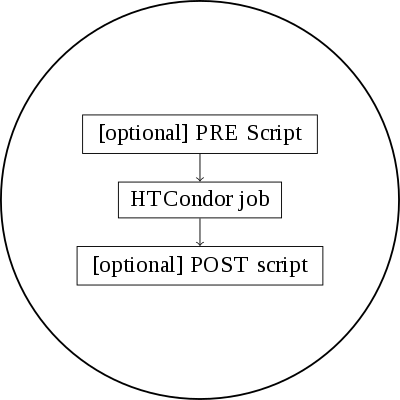
\includegraphics{user-man/dagman-node.eps}
\caption{\label{fig:dagman-node}One Node within a DAG}
\end{figure}

More than one HTCondor job may belong to a single node.
All HTCondor jobs within a node must be within
a single cluster, as given by the job ClassAd attribute \Attr{ClusterId}.
%In addition,
%all jobs within the single cluster must use the same log file.
%Separate nodes within a DAG may use different log files.

\emph{DAGMan enforces the dependencies within a DAG
using the events recorded in a separate
file that is specified by the default configuration.
If the exact same DAG were to be submitted more than once,
such that these DAGs were running at the same time,
expected them to fail in unpredictable and unexpected ways.
They would all be using the same single file to enforce dependencies. }

As DAGMan schedules and submits jobs within nodes to HTCondor,
these jobs are defined to succeed or fail based on their
return values.
This success or failure is propagated in well-defined ways to the level of
a node within a DAG.
Further progression of computation
(towards completing the DAG)
is based upon the success or failure of nodes.

The failure of a single job within a cluster
of multiple jobs
(within a single node)
causes the entire cluster of jobs to fail.
Any other jobs within the failed cluster of jobs are
immediately removed.
Each node within a DAG may be further constrained  to succeed or fail
based upon the return values of a PRE script and/or a POST script.

%%%%%%%%%%%%%%%%%%%%%%%%%%%%%%%%%%%%%%%
\subsection{The DAG Input File: Basic Commands}
%%%%%%%%%%%%%%%%%%%%%%%%%%%%%%%%%%%%%%%
\index{DAGMan!DAG input file}

The input file used by DAGMan is called a DAG input file.
It specifies the nodes of the DAG as well as the dependencies
that order the DAG.
All items are optional, except that there must be at least one \Arg{JOB}
item.

Comments may be placed in the DAG input file.
The pound character (\verb@#@) as the first character on a
line identifies the line as a comment.
Comments do not span lines.

A simple diamond-shaped DAG, as shown in
Figure~\ref{fig:dagman-diamond}
is presented as a starting point for examples.
This DAG contains 4 nodes.

\begin{figure}[hbt]
\centering
\includegraphics{user-man/dagman-diamond.eps}
\caption{\label{fig:dagman-diamond}Diamond DAG}
\end{figure}


A very simple DAG input file for this diamond-shaped DAG is

\footnotesize
\begin{verbatim}
    # File name: diamond.dag
    #
    JOB  A  A.condor 
    JOB  B  B.condor 
    JOB  C  C.condor	
    JOB  D  D.condor
    PARENT A CHILD B C
    PARENT B C CHILD D
\end{verbatim}
\normalsize

A set of basic commands appearing in a DAG input file is described below.


%%%%%%%%%%%%%%%%%%%%%%%%%%%%%%%%%%%%%%%
\subsubsection{\label{sec:dagman_job_command}JOB}
\label{dagman:JOB}
\index{DAG input file!JOB command}

The \Arg{JOB} command specifies an HTCondor job.
The syntax used for each \Arg{JOB} command is

\Opt{JOB} \Arg{JobName} \Arg{SubmitDescriptionFileName}
\oOptArg{DIR}{directory} \oOpt{NOOP} \oOpt{DONE}

A \Arg{JOB} entry maps a \Arg{JobName} to an HTCondor submit description file.
The \Arg{JobName} uniquely identifies nodes within the
DAG input file and in output messages.
Each node name, given by \Arg{JobName}, within the DAG must be unique.
The \Arg{JOB} entry must appear within the DAG input file before
other items that reference the node.

The keywords \Arg{JOB}, \Arg{DIR}, \Arg{NOOP}, and \Arg{DONE}
are not case sensitive.
Therefore, \Arg{DONE}, \Arg{Done}, and \Arg{done} are all equivalent.
The values defined for \Arg{JobName} and \Arg{SubmitDescriptionFileName}
are case sensitive, as file names 
in a file system are case sensitive.
The \Arg{JobName} can be any string that contains no white space, except
for the strings \Arg{PARENT} and \Arg{CHILD} (in upper, lower, or mixed
case).

Note that \Arg{DIR}, \Arg{NOOP}, and \Arg{DONE}, if used, must appear
in the order shown above.

The optional \Arg{DIR} keyword specifies a working directory
for this node,
from which the HTCondor job will be submitted,
and from which a \Arg{PRE} and/or
\Arg{POST} script will be run.
If a relative directory is specified, it is relative to the current working 
directory as the DAG is submitted.
Note that a DAG containing \Arg{DIR} specifications cannot
be run in conjunction with the \Arg{-usedagdir} command-line
argument to \Condor{submit\_dag}.
A "full" rescue DAG generated by a DAG run with the \Arg{-usedagdir} argument
will contain DIR specifications, so such a rescue DAG must be run
\emph{without} the \Arg{-usedagdir} argument.  (Note that "full"
rescue DAGs are no longer the default.)

\label{dagman:NOOP}
The optional \Arg{NOOP} keyword identifies that the HTCondor job within
the node is not to be submitted to HTCondor.
This optimization is useful in cases such as debugging a complex DAG structure,
where some of the individual jobs are long-running.
For this debugging of structure,
some jobs are marked as \Arg{NOOP}s, and
the DAG is initially run to verify that the control flow through
the DAG is correct.
The \Arg{NOOP} keywords are then removed before submitting the DAG.
Any PRE and POST scripts
for jobs specified with \Arg{NOOP} \emph{are} executed;
to avoid running the PRE and POST scripts, comment them out.
The job that is not submitted to HTCondor is given a return value that indicates
success, such that the node may also succeed.
Return values of any 
PRE and POST scripts may still cause the node to fail.
Even though the job specified with \Arg{NOOP} is not submitted,
its submit description file must exist;
the log file for the job is used, 
because DAGMan generates dummy submission and termination events for the job.

The optional \Arg{DONE} keyword identifies a node as being already
completed.
This is mainly used by Rescue DAGs generated by DAGMan itself,
in the event of a failure to complete the workflow.
Nodes with the \Arg{DONE} keyword are not executed when the Rescue DAG is run,
allowing the workflow to pick up from the previous endpoint.  Users
should generally not use the \Arg{DONE} keyword.
The \Arg{NOOP} keyword is more flexible in avoiding
the execution of a job within a node.
Note that, for any node marked \Arg{DONE} in a DAG, all of
its parents must also be marked \Arg{DONE}; 
otherwise, a fatal error will result.
The \Arg{DONE} keyword applies to the entire node.
A node marked with \Arg{DONE} will not have a PRE or POST script run,
and the HTCondor job will not be submitted.

%%%%%%%%%%%%%%%%%%%%%%%%%%%%%%%%%%%%%%%
\subsubsection{\label{sec:dagman_data_command}DATA}
\label{dagman:DATA}
\index{DAG input file!DATA command}

As of version 8.3.5, \Condor{dagman} no longer supports DATA nodes.

%%%%%%%%%%%%%%%%%%%%%%%%%%%%%%%%%%%%%%%
\subsubsection{\label{sec:dagman_parent_child_command}PARENT \Dots CHILD}
\label{dagman:ParentChild}
\index{DAG input file!PARENT \Dots CHILD command}

The \Arg{PARENT} \Arg{CHILD} command specifies the
dependencies within the DAG.
\index{DAGMan!describing dependencies}
Nodes are parents and/or children within the DAG.
A parent node must be completed successfully before
any of its children may be started.
A child node may only be started once
all its parents have successfully completed.

The syntax used for each dependency (PARENT/CHILD) command is

\Opt{PARENT} \Arg{ParentJobName\Dots} \Opt{CHILD} \Arg{ChildJobName\Dots}

The \Arg{PARENT} keyword is followed by one or more
\Arg{ParentJobName}s.
The \Arg{CHILD} keyword is followed by one or more
\Arg{ChildJobName}s.
Each child job depends on every parent job within the line.
A single line in the input file can specify the dependencies from one or more
parents to one or more children.
The diamond-shaped DAG example may specify the dependencies with
\begin{verbatim}
PARENT A CHILD B C
PARENT B C CHILD D
\end{verbatim}
An alternative specification for the diamond-shaped DAG
may specify some or all of the dependencies on separate lines:
\begin{verbatim}
PARENT A CHILD B C
PARENT B CHILD D
PARENT C CHILD D
\end{verbatim}

As a further example, the line
\begin{verbatim}
PARENT p1 p2 CHILD c1 c2
\end{verbatim}
produces four dependencies:
\begin{enumerate}
\item{\verb@p1@ to \verb@c1@}
\item{\verb@p1@ to \verb@c2@}
\item{\verb@p2@ to \verb@c1@}
\item{\verb@p2@ to \verb@c2@}
\end{enumerate}

%%%%%%%%%%%%%%%%%%%%%%%%%%%%%%%%%%%%%%%
\subsubsection{\label{sec:dagman_script_command}SCRIPT}
\label{dagman:SCRIPT}
\index{DAG input file!SCRIPT command}
\index{DAGMan!PRE and POST scripts}

The optional \Arg{SCRIPT} command specifies
processing that is done either before a job within
a node is submitted
or after a job within a node completes its execution.
\index{DAGMan!PRE script}
Processing done before a job is submitted is
called a \Arg{PRE} script.
Processing done after a job completes its execution is
\index{DAGMan!POST script}
called a \Arg{POST} script.
Note that the executable specified does not necessarily
have to be a shell script (Unix) or batch file (Windows);
but it should be relatively light weight because it will
be run directly on the submit machine, not submitted as
an HTCondor job.

The syntax used for each \Arg{PRE} or \Arg{POST} command is

\Opt{SCRIPT} \oOptArg{DEFER}{status time}
\Opt{PRE} \Arg{JobName}|\Opt{ALL\_NODES} \Arg{ExecutableName}
\oArg{arguments}

\Opt{SCRIPT} \oOptArg{DEFER}{status time}
\Opt{POST}  \Arg{JobName}|\Opt{ALL\_NODES} \Arg{ExecutableName}
\oArg{arguments}

The \Arg{SCRIPT} command uses
the \Arg{PRE} or \Arg{POST} keyword,
which specifies the relative timing of when the script is to be run.
The \Arg{JobName} identifies the node to which the script is attached.
The \Arg{ExecutableName}
specifies the executable (e.g., shell script or batch file) to be executed, 
and may not contain spaces.
The optional \Arg{arguments} are command line arguments to the script,
and spaces delimit the arguments.
Both \Arg{ExecutableName} and optional \Arg{arguments} are
case sensitive.

Scripts are executed on the submit machine;
the submit machine is not necessarily
the same machine upon which the node's job is run.
Further, a single cluster of HTCondor jobs may be
spread across several machines.

The optional \Arg{DEFER} feature causes a retry of only the script,
if the execution of the script exits with the
exit code given by \Arg{status}.
The retry occurs after at least \Arg{time} seconds, 
rather than being considered failed.  
While waiting for the retry,
the script does not count against a \Arg{maxpre} or \Arg{maxpost} limit.
The ordering of the \Arg{DEFER} feature within the \Arg{SCRIPT} 
specification is fixed.
It must come directly after the \Arg{SCRIPT} keyword;
this is done to avoid backward compatibility issues for any
DAG with a \Arg{JobName} of DEFER.

A PRE script is commonly used
to place files in a staging area for the jobs to use.
A POST script is commonly used
to clean up or remove files once jobs are finished running.
An example uses PRE and POST scripts to stage files
that are stored on tape.
The PRE script reads compressed input files from the tape drive,
uncompresses them, and places the resulting files in the current directory.
The HTCondor jobs can then use these files,
producing output files.
The POST script compresses the output files, writes them out to
the tape, and then removes both the staged files and the output files.

If the PRE script fails, 
then the HTCondor job associated with the node is not submitted,
and (as of version 8.5.4) the POST
script is not run either (by default).
However, if the job is submitted, and there is a POST script, the POST
script is always run once the job finishes.
(The behavior when the PRE script fails may
may be changed to run the POST script
by setting configuration variable \MacroNI{DAGMAN\_ALWAYS\_RUN\_POST} 
to \Expr{True} or by passing the \Opt{-AlwaysRunPost}
argument to \Condor{submit\_dag}.)

Progress towards completion of the DAG is based upon
the success of the nodes within the DAG.
The success of a node is based upon the success of 
the job(s), PRE script, and POST script.
A job, PRE script, or POST script with an exit value not equal to 0 is
considered failed.  
\Bold{The exit value of whatever component of the node was run last
determines the success or failure of the node.}
Table~\ref{NodeS-F} lists the definition of node success and
failure for all variations of script and job success and failure,
when \MacroNI{DAGMAN\_ALWAYS\_RUN\_POST} is set to \Expr{False}.
In this table, a dash (\Expr{-}) represents the case where a script
does not exist for the DAG, \Bold{S} represents success, 
and  \Bold{F} represents failure.

Table~\ref{NodeS-F-ARP} lists the definition of node success and
failure only for the cases where the PRE script fails,
when \MacroNI{DAGMAN\_ALWAYS\_RUN\_POST} is set to \Expr{True}.

%An exit value not equal to 0 indicates program failure,
%except as indicated by the \Arg{PRE\_SKIP} command:
%if a PRE script exits with the PRE\_SKIP value, 
%then the node succeeds and the job and the POST script are both skipped.  
%It is therefore important that a
%successful program return the exit value 0. 
%It is good practice to always
%explicitly specify a return value in the PRE script,
%returning 0 in the case of success.
%Otherwise,
%the return code of the last completed process is returned,
%which can lead to unexpected results. 

\begin{center}
\begin{table}[hbt]
\begin{tabular}{|c|c|c|c|} \hline
PRE  & JOB & POST & \Bold{Node}  \\
\hline
-  & S & - & \Bold{S}  \\
-  & F & - & \Bold{F}  \\
-  & S & S & \Bold{S}  \\
-  & S & F & \Bold{F}  \\
-  & F & S & \Bold{S}  \\
-  & F & F & \Bold{F}  \\
S  & S & - & \Bold{S}  \\
S  & F & - & \Bold{F}  \\
S  & S & S & \Bold{S}  \\
S  & S & F & \Bold{F}  \\
S  & F & S & \Bold{S}  \\
S  & F & F & \Bold{F}  \\
F  & not run & - & \Bold{F}  \\
F  & not run & not run & \Bold{F}  \\
\end{tabular}
\caption{\label{NodeS-F}Node success or failure definition with \Expr{DAGMAN\_ALWAYS\_RUN\_POST = False (the default)} }
\end{table}
\end{center}

\begin{center}
\begin{table}[hbt]
\begin{tabular}{|c|c|c|c|} \hline
PRE  & JOB & POST & \Bold{Node}  \\
F  & not run & - & \Bold{F}  \\
F  & not run & S & \Bold{S}  \\
F  & not run & F & \Bold{F}  \\
\hline
\end{tabular}
\caption{\label{NodeS-F-ARP}Node \Bold{S}uccess or \Bold{F}ailure definition with \Expr{ DAGMAN\_ALWAYS\_RUN\_POST = True} }
\end{table}
\end{center}

\Bold{Special script argument macros}

The five macros \Expr{\$JOB}, \Expr{\$RETRY}, \Expr{\$MAX\_RETRIES}, 
\Expr{\$DAG\_STATUS} and \Expr{\$FAILED\_COUNT} can be used within the
DAG input file as arguments passed to a PRE or POST script. 
The three macros \Expr{\$JOBID}, \Expr{\$RETURN}, 
and \Expr{\$PRE\_SCRIPT\_RETURN} can
be used as arguments to POST scripts.
The use of these variables is limited to being used
as an individual command
line \Arg{argument} to the script,
surrounded by spaces, in order to cause the substitution of the
variable's value.

The special macros are as follows:

\begin{itemize}
\item \index{DAGMan!JOB@\verb^$JOB^ value}
\Expr{\$JOB} evaluates to the (case sensitive) string
defined for \Arg{JobName}.

\item \index{DAGMan!RETRY@\verb^$RETRY^ value}
\Expr{\$RETRY} evaluates to an 
integer value set to 0 the first time a node is run,
and is incremented each time the node is retried. 
See section~\ref{dagman:retry} for the description of how to cause
nodes to be retried. 

\item \index{DAGMan!MAX_RETRIES@\verb^$MAX_RETRIES^ value}
\Expr{\$MAX\_RETRIES} evaluates to an integer value set 
to the maximum number of retries for the node.
See section~\ref{dagman:retry} for the description of how to cause
nodes to be retried.  
If no retries are set for the node,
\Expr{\$MAX\_RETRIES} will be set to 0.

\item \index{DAGMan!JOBID@\verb^$JOBID^ value}
\index{job ID!defined for a DAGMan node job}
\index{job!job ID!defined for a DAGMan node job}
\Expr{\$JOBID} (for POST scripts only)
evaluates to a representation of the HTCondor job ID of the node job.
It is the value of the job ClassAd attribute \Attr{ClusterId},
followed by a period,
and then followed by the value of the job ClassAd attribute \Attr{ProcId}.
An example of a job ID might be 1234.0.
For nodes with multiple jobs in the same cluster,
the \Attr{ProcId} value is the one of the last job within the cluster.

\item \index{DAGMan!return@\verb^$RETURN^ value}
\Expr{\$RETURN} (for POST scripts only) variable evaluates to
the return value of the 
HTCondor job, if there is a single job within a cluster.
With multiple jobs within the same cluster,
there are two cases to consider.
In the first case, all jobs within the cluster are successful;
the value of \Expr{\$RETURN} will be 0, indicating success.
In the second case,
one or more jobs from the cluster fail.
When \Condor{dagman} sees the first terminated event for a job that failed,
it assigns that job's return value as the value of \Expr{\$RETURN},
and it attempts to remove all remaining jobs within the cluster.
Therefore, if multiple jobs in the cluster fail with different exit codes,
a race condition determines which exit code gets assigned to \Expr{\$RETURN}.

A job that dies due to a signal is reported with a \Expr{\$RETURN} value
representing the additive inverse of the signal number.
For example, SIGKILL (signal 9) is reported as -9.
A job whose batch system submission fails is reported as -1001.
A job that is externally removed from the batch system queue
(by something other than \Condor{dagman}) is reported as -1002.

\item \index{DAGMan!PRE_SCRIPT_RETURN@\verb^$PRE_SCRIPT_RETURN^ value}
\Expr{\$PRE\_SCRIPT\_RETURN} (for POST scripts only)
variable evaluates to the return value of the PRE script of a node, 
if there is one.
If there is no PRE script, this value will be -1.
If the node job was skipped because of failure of the PRE script,
the value of \Expr{\$RETURN} will be -1004
and the value of \Expr{\$PRE\_SCRIPT\_RETURN} will be the exit value
of the PRE script;
the POST script can use this to see if the PRE script exited
with an error condition, and assign success or failure to the node, as
appropriate.

%\item \Expr{\$DAG\_STATUS} and \Expr{\$FAILED\_COUNT} are documented in
%section ~\ref{sec:DAGFinalNode} below.
%\begin{itemize}
\index{DAGMan!DAG_STATUS@\verb^$DAG_STATUS^ value}
\item \Env{\$DAG\_STATUS} is the status of the DAG.
Note that this macro's value and definition is unrelated to the attribute 
named \Attr{DagStatus} as defined for use in a node status file.
This macro's value is the same as the job ClassAd attribute \Attr{DAG\_Status}
that is defined within the \Condor{dagman} job's ClassAd.
This macro may have the following values:
\begin{itemize}
\item 0: OK
\item 1: error; an error condition different than those listed here
\item 2: one or more nodes in the DAG have failed
\item 3: the DAG has been aborted by an ABORT-DAG-ON specification
\item 4: removed; the DAG has been removed by \Condor{rm}
\item 5: cycle; a cycle was found in the DAG
\item 6: halted; the DAG has been halted (see section ~\ref{sec:DagSuspend})
\end{itemize}

\index{DAGMan!FAILED_COUNT@\verb^$FAILED_COUNT^ value}
\item \Env{\$FAILED\_COUNT} is defined by the number of nodes that have failed in the
DAG.

\end{itemize}


\Bold{Examples that use PRE or POST scripts}

Examples use the diamond-shaped DAG.
A first example uses a PRE script to expand a compressed file 
needed as input to each of the HTCondor jobs of nodes B and C.
The DAG input file:

\footnotesize
\begin{verbatim}
    # File name: diamond.dag
    #
    JOB  A  A.condor 
    JOB  B  B.condor 
    JOB  C  C.condor	
    JOB  D  D.condor
    SCRIPT PRE  B  pre.csh $JOB .gz
    SCRIPT PRE  C  pre.csh $JOB .gz
    PARENT A CHILD B C
    PARENT B C CHILD D
\end{verbatim}
\normalsize

The script \File{pre.csh} uses its command line arguments to form the file name
of the compressed file.
The script contains

\begin{verbatim}
  #!/bin/csh
  gunzip $argv[1]$argv[2]
\end{verbatim}

Therefore, the PRE script invokes  
\begin{verbatim}
  gunzip B.gz
\end{verbatim}
for node B, which uncompresses file \File{B.gz},
placing the result in file \File{B}.

A second example uses the \Expr{\$RETURN} macro.
The DAG input file contains the POST script specification:
\begin{verbatim}
  SCRIPT POST A stage-out job_status $RETURN 
\end{verbatim}
If the HTCondor job of node A exits with the value -1,
the POST script is invoked as
\begin{verbatim}
  stage-out job_status -1
\end{verbatim}

The slightly different example POST script specification
in the DAG input file
\begin{verbatim}
  SCRIPT POST A stage-out job_status=$RETURN 
\end{verbatim}
invokes the POST script with
\begin{verbatim}
  stage-out job_status=$RETURN
\end{verbatim}

This example shows that when
there is no space between the \Expr{=} sign and the variable \Expr{\$RETURN},
there is no substitution of the macro's value.

%%%%%%%%%%%%%%%%%%%%%%%%%%%%%%%%%%%%%%%
\subsubsection{\label{sec:dagman_pre_skip_command}PRE\_SKIP}
\label{dagman:PRE-SKIP}
\index{DAG input file!PRE\_SKIP command}
\index{DAGMan!skipping node execution}

The behavior of DAGMan with respect to node success or failure can
be changed with the addition of a \Arg{PRE\_SKIP} command. 
A \Arg{PRE\_SKIP} line within the DAG input file uses the syntax: 

\Opt{PRE\_SKIP} \Arg{JobName}|\Opt{ALL\_NODES} \Arg{non-zero-exit-code}

The PRE script of a node identified by \Arg{JobName} that exits with the value 
given by \Arg{non-zero-exit-code}
skips the remainder of the node entirely.  
Neither the job associated with the node nor
the POST script will be executed,
and the node will be marked as successful.

% $ % this comment just has a dollar sign so that emacs will not think
%	  we're inside of a math section and will draw things more nicely

%%%%%%%%%%%%%%%%%%%%%%%%%%%%%%%%%%%%%%%
\subsection{\label{sec:DAG-command_order}Command Order}
\label{dagman:command order}
\index{DAG input file!command order}
\index{DAGMan!command order}

As of version 8.5.6, commands referencing a \Arg{JobName} \emph{can}
come before the JOB command defining that \Arg{JobName}.

For example, the command sequence
\begin{verbatim}
SCRIPT PRE NodeA foo.pl
VARS NodeA state="Wisconsin"
JOB NodeA bar.sub
\end{verbatim}
is now legal (it would have been illegal in 8.5.5 and all previous
versions).

%%%%%%%%%%%%%%%%%%%%%%%%%%%%%%%%%%%%%%%
\subsection{Node Job Submit File Contents}
%%%%%%%%%%%%%%%%%%%%%%%%%%%%%%%%%%%%%%%
\index{DAGMan!node job submit description file}

Each node in a DAG may use a unique submit description file.
A key limitation is that
each HTCondor submit description file must submit jobs
described by a single cluster number;
DAGMan cannot deal with a submit description file producing
multiple job clusters.

Consider again the diamond-shaped DAG example, 
where each node job uses the same submit description file.

\begin{verbatim}
    # File name: diamond.dag
    #
    JOB  A  diamond_job.condor 
    JOB  B  diamond_job.condor 
    JOB  C  diamond_job.condor	
    JOB  D  diamond_job.condor
    PARENT A CHILD B C
    PARENT B C CHILD D
\end{verbatim}

Here is a sample HTCondor submit description file
for this DAG:

\index{DAGMan!example submit description file}
\begin{verbatim}
    # File name: diamond_job.condor
    #
    executable   = /path/diamond.exe
    output       = diamond.out.$(cluster)
    error        = diamond.err.$(cluster)
    log          = diamond_condor.log
    universe     = vanilla
    queue
\end{verbatim}

Since each node uses the same HTCondor submit description file,
this implies that each node within the DAG runs the
same job.
The \MacroUNI{Cluster} macro
produces unique file names for each job's output.

\index{ClassAd job attribute!DAGParentNodeNames}
\index{DAGParentNodeNames!job ClassAd attribute}
The job ClassAd attribute \Attr{DAGParentNodeNames} is also available
for use within the submit description file. 
It defines a comma separated list of each \Arg{JobName}
which is a parent node of this job's node.
This attribute may be used in the \SubmitCmd{arguments} command
for all but scheduler universe jobs.
For example, if the job has two parents, with \Arg{JobName}s B and C,
the submit description file command
\begin{verbatim}
arguments = $$([DAGParentNodeNames])
\end{verbatim}
will pass the string \AdStr{B,C} as the command line argument when invoking
the job.

%%%%%%%%%%%%%%%%%%%%%%%%%%%%%%%%%%%%%%%
\subsection{\label{dagman:submitdag}DAG Submission}
%%%%%%%%%%%%%%%%%%%%%%%%%%%%%%%%%%%%%%%
\index{DAGMan!DAG submission}

A DAG is submitted using the tool \Condor{submit\_dag}.
The manual
page~\pageref{man-condor-submit-dag}
details the command.
The simplest of DAG submissions has the syntax

\Condor{submit\_dag} \Arg{DAGInputFileName}

and the current working directory contains the DAG input file.

The diamond-shaped DAG example may be submitted with

\begin{verbatim}
condor_submit_dag diamond.dag
\end{verbatim}

Do not submit the same DAG, with same DAG input file, 
from within the same directory, 
such that more than one of this same DAG is running at the same time.
It will fail in an unpredictable manner,
as each instance of this same DAG will attempt to use the same
file to enforce dependencies.
 
To increase robustness and guarantee recoverability, the 
\Condor{dagman} process is run as an HTCondor job.
As such, it needs a submit description file.
\Condor{submit\_dag} generates this needed submit description file,
naming it by appending \File{.condor.sub} to the name of the DAG input file.
This submit description file may be edited if the DAG is submitted with

\begin{verbatim}
condor_submit_dag -no_submit diamond.dag
\end{verbatim}
causing \Condor{submit\_dag} to create the submit description file,
but not submit \Condor{dagman} to HTCondor.
To submit the DAG, once the submit description file is edited,
use

\begin{verbatim}
condor_submit diamond.dag.condor.sub
\end{verbatim}

Submit machines with limited resources are supported by
command line options that place limits on the submission and handling 
of HTCondor jobs and PRE and POST scripts. 
Presented here are descriptions of the command line options
to \Condor{submit\_dag}.
These same limits can be set in configuration.
Each limit is applied within a single DAG.

%%%%%%%%%%%%%%%%%%%%%%%%%%%%%%%%%%%%%%%
\subsubsection{\label{sec:DAG-throttling}DAG Throttling}
\index{DAGMan!throttling}

\Bold{Total nodes/clusters:}
The \Opt{-maxjobs} option 
specifies the maximum number of clusters that \Condor{dagman}
can submit at one time.
Since each node corresponds to a single cluster,
this limit restricts the number of nodes that can be submitted (in the
HTCondor queue) at a time.
It is commonly used when
there is a limited amount of input file staging capacity.
As a specific example, consider a case where each node represents
a single HTCondor proc that requires 4 MB of input files,
and the proc will run in a directory with a volume of 100 MB
of free space.
Using the argument \Opt{-maxjobs 25} guarantees that a maximum
of 25 clusters, using a maximum of 100 MB of space,
will be submitted to HTCondor at one time.
(See the \Condor{submit\_dag} man page (~\ref{man-condor-submit-dag})
for more information.  Also see the equivalent
\Macro{DAGMAN\_MAX\_JOBS\_SUBMITTED} configuration option
(~\ref{param:DAGManMaxJobsSubmitted}).)

\Bold{Idle procs:}
The number of idle procs within a given DAG can be limited with
the optional command line argument \Opt{-maxidle}. 
\Condor{dagman} will not submit any more node jobs 
until the number of idle procs in the DAG goes below this
specified value,
even if there are ready nodes in the DAG.
This allows \Condor{dagman} to submit jobs in a way that adapts to
the load on the HTCondor pool at any given time.  If the pool is
lightly loaded, \Condor{dagman} will end up submitting more jobs;
if the pool is heavily loaded, \Condor{dagman} will submit fewer jobs.
(See the \Condor{submit\_dag} man page (~\ref{man-condor-submit-dag})
for more information.  Also see the equivalent
\Macro{DAGMAN\_MAX\_JOBS\_IDLE} configuration option
(~\ref{param:DAGManMaxJobsIdle}).)

Note that the \Opt{-maxjobs} option applies to counts of
\emph{clusters}, whereas the \Opt{-maxidle} option
applies to counts of \emph{procs}.  Unfortunately, this can
be a bit confusing.  Of course, if none of your submit files
create more than one proc, the distinction doesn't matter.
For example, though, a node job submit file that queues
5 procs will count as one for \Opt{-maxjobs}, but five
for \Opt{-maxidle} (if all of the procs are idle).

\Bold{Subsets of nodes:}
Node submission can also be throttled in a finer-grained manner by
grouping nodes into categories.  See section ~\ref{sec:DAG-node-category}
for more details.

\Bold{PRE/POST scripts:}
Since PRE and POST scripts run on the submit machine,
it may be desirable to limit the number of PRE or POST scripts running
at one time.
The optional \Opt{-maxpre} command line argument limits the number of PRE
scripts that may be running at one time,
and the optional \Opt{-maxpost} command line argument limits the number
of POST scripts that may be running at one time.
(See the \Condor{submit\_dag} man page (~\ref{man-condor-submit-dag})
for more information.  Also see the equivalent
\Macro{DAGMAN\_MAX\_PRE\_SCRIPTS} (~\ref{param:DAGManMaxPreScripts}) and
\Macro{DAGMAN\_MAX\_POST\_SCRIPTS} (~\ref{param:DAGManMaxPostScripts})
configuration options.)

%%%%%%%%%%%%%%%%%%%%%%%%%%%%%%%%%%%%%%%
\subsection{\label{sec:DAGPaths}File Paths in DAGs}
%%%%%%%%%%%%%%%%%%%%%%%%%%%%%%%%%%%%%%%
\index{DAGMan!file paths in DAGs}

\Condor{dagman} assumes that all relative paths in a
DAG input file and the associated HTCondor submit description files
are relative to the current
working directory when \Condor{submit\_dag} is run.  
This works well for submitting a single DAG.
It presents problems when multiple independent DAGs are submitted
with a single invocation of \Condor{submit\_dag}.
Each of these independent DAGs would logically be in its own directory, 
such that it could be run or tested independent of other DAGs.
Thus, all references to files will be designed to be relative to
the DAG's own directory.

%Note that 
%relative paths in submit description files can be modified by the submit command
%\SubmitCmd{initialdir}; 
%see the \Condor{submit} manual page at ~\ref{man-condor-submit} 
%for more details on this command.
%The remainder of this discussion ignores \SubmitCmd{initialdir}.

Consider an example DAG within a directory named \File{dag1}.
There would be a DAG input file, named \File{one.dag} for this example.
Assume the contents of this DAG input file specify a node job with
\begin{verbatim}
  JOB A  A.submit
\end{verbatim}
Further assume that partial contents of submit description file 
\File{A.submit} specify
\begin{verbatim}
  executable = programA
  input      = A.input
\end{verbatim}

Directory contents are 
\begin{verbatim}
    dag1 (directory)
          one.dag
          A.submit
          programA
          A.input
\end{verbatim}

All file paths are correct relative to the \File{dag1} directory.
Submission of this example DAG sets the current working directory
to \File{dag1} and invokes \Condor{submit\_dag}:
\begin{verbatim}
  cd dag1
  condor_submit_dag one.dag
\end{verbatim}

Expand this example such that there are now two independent DAGs,
and each is contained within its own directory. 
For simplicity, assume that the DAG in \File{dag2} has remarkably
similar files and file naming as the DAG in \File{dag1}.
Assume that the directory contents are 
\begin{verbatim}
    parent (directory)
         dag1 (directory)
               one.dag
               A.submit
               programA
               A.input
         dag2 (directory)
               two.dag
               B.submit
               programB
               B.input
\end{verbatim}

The goal is to use a single invocation of \Condor{submit\_dag}
to run both dag1 and dag2.
The invocation
\begin{verbatim}
  cd parent
  condor_submit_dag dag1/one.dag dag2/two.dag
\end{verbatim}
\emph{does not work}.
Path names are now relative to \File{parent}, 
which is \emph{not} the desired behavior.

The solution is 
the \Arg{-usedagdir} command line argument to \Condor{submit\_dag}.
This feature runs each DAG as if \Condor{submit\_dag} had been run 
in the directory in which the relevant DAG file exists.
A working invocation is
\begin{verbatim}
  cd parent
  condor_submit_dag -usedagdir dag1/one.dag dag2/two.dag
\end{verbatim}

Output files will be placed in the correct directory, and
the \File{.dagman.out} file will also be in the correct directory.
A Rescue DAG file will be written to
the current working directory, which is the directory when
\Condor{submit\_dag} is invoked.
The Rescue DAG should be run from that same current working directory.
The Rescue DAG includes all the path information necessary to
run each node job in the proper directory.

%If all paths in the DAG input file(s) and the relevant submit
%description files are absolute,
%the \Arg{-usedagdir} argument is not needed;
%however, using absolute paths is NOT generally a good idea.

%For a DAG that \emph{does not} use \Arg{-usedagdir}, 
%relative paths can still work for multiple DAGs, 
%if all file paths are given relative to
%the current working directory as \Condor{submit\_dag} is executed.
%This implies that DAGs in separate directories
%cannot be submitted from their own directories;
%submission only works from the parent directory the paths are set up for.

Use of \Arg{-usedagdir} does \emph{not} work in conjunction with
a JOB node specification within the DAG input file using
the \Arg{DIR} keyword.
Using both will be detected and generate an error. 

%%%%%%%%%%%%%%%%%%%%%%%%%%%%%%%%%%%%%%%
\subsection{\label{sec:DAGMonitoring}DAG Monitoring and DAG Removal}
%%%%%%%%%%%%%%%%%%%%%%%%%%%%%%%%%%%%%%%
\index{DAGMan!DAG monitoring}
\index{DAGMan!DAG removal}

%TEMP -- this section needs lots of improvement... (dagman.out, node
% status file, jobstate.log file, halt file, etc.)

After submission, the progress of the DAG can be monitored
by looking at the job event log file(s),
observing the e-mail that job submission to HTCondor causes,
or by using \Condor{q} \Arg{-dag}.

There is also a large amount of information logged in an extra file.
The name of this extra file is produced by appending
\File{.dagman.out} to the name of the DAG input file; 
for example, if the DAG input file is \File{diamond.dag}, 
this extra file is named \File {diamond.dag.dagman.out}.
If this extra file grows too large, limit its size
with the configuration variable \Macro{MAX\_DAGMAN\_LOG},
as defined in section~\ref{param:MaxSubsysLog}.
The \File{dagman.out} file is an important resource for
debugging; save this file if a problem occurs. 
The \File{dagman.out} is appended to, rather than overwritten, 
with each new DAGMan run.

To remove an entire DAG, consisting of the \Condor{dagman} job, 
plus any jobs submitted to HTCondor,
remove the \Condor{dagman} job by running \Condor{rm}.
For example,
%TEMP -- example needs to be changed to match current condor_q
\footnotesize
\begin{verbatim}
% condor_q
-- Submitter: turunmaa.cs.wisc.edu : <128.105.175.125:36165> : turunmaa.cs.wisc.edu
 ID      OWNER          SUBMITTED     RUN_TIME ST PRI SIZE CMD
  9.0   taylor         10/12 11:47   0+00:01:32 R  0   8.7  condor_dagman -f -
 11.0   taylor         10/12 11:48   0+00:00:00 I  0   3.6  B.out
 12.0   taylor         10/12 11:48   0+00:00:00 I  0   3.6  C.out

    3 jobs; 2 idle, 1 running, 0 held

% condor_rm 9.0
\end{verbatim}
\normalsize

When a \Condor{dagman} job is removed, all node jobs (including sub-DAGs)
of that \Condor{dagman} will be removed by the \Condor{schedd}.  As of version
8.5.8, the default is that \Condor{dagman} itself also removes the
node jobs (to fix a race condition that could result in "orphaned"
node jobs).  (The \Condor{schedd} has to remove the node jobs to deal with
the case of removing a \Condor{dagman} job that has been held.)

The previous behavior of \Condor{dagman} itself \emph{not} removing
the node jobs can be restored by setting the
\MacroNI{DAGMAN\_REMOVE\_NODE\_JOBS} configuration macro
(see ~\ref{param:DAGManRemoveNodeJobs})
to \Expr{False}.  This will decrease the load on the \Condor{schedd},
at the cost of allowing the possibility of "orphaned" node jobs.

A removed DAG will be considered failed unless the
DAG has a FINAL node that succeeds.

%TEMP -- this needs to be fixed/clarified
In the case where a
machine is scheduled to go down,
DAGMan will clean up memory and exit.
However, it will leave any submitted jobs
in the HTCondor queue.

%%%%%%%%%%%%%%%%%%%%%%%%%%%%%%%%%%%%%%%
\subsection{\label{sec:DagSuspend}Suspending a Running DAG}
%%%%%%%%%%%%%%%%%%%%%%%%%%%%%%%%%%%%%%%
\index{DAGMan!suspending a running DAG}

It may be desired to temporarily suspend a running DAG.
For example, the load may be high on the submit machine,
and therefore it is desired to prevent DAGMan from
submitting any more jobs until the load goes down.
There are two ways to suspend (and resume) a running DAG.

\begin{itemize}
\item Use \Condor{hold}/\Condor{release} on the \Condor{dagman} job.

After placing the \Condor{dagman} job on hold,
no new node jobs will be submitted,
and no PRE or POST scripts will be run.
Any node jobs already in the HTCondor queue will continue undisturbed.
Any running PRE or POST scripts will be killed.
If the \Condor{dagman} job is left on hold,
it will remain in the HTCondor queue after all of the currently running
node jobs are finished.
To resume the DAG, use \Condor{release} on the \Condor{dagman} job.

Note that while the \Condor{dagman} job is on hold,
no updates will be made to the \File{dagman.out} file.

\item Use a DAG halt file.

The second way of suspending a DAG uses the existence of a specially-named
file to change the state of the DAG.
When in this halted state,
no PRE scripts will be run, and no node jobs will be submitted.  
Running node jobs will continue undisturbed.
A halted DAG will still run POST scripts,
and it will still update the \File{dagman.out} file.
This differs from behavior of a DAG that is held.
Furthermore, a halted DAG will not remain in the queue indefinitely;
when all of the running node jobs have finished, 
DAGMan will create a Rescue DAG and exit.

To resume a halted DAG, remove the halt file.

The specially-named file must be placed in the same directory
as the DAG input file.
The naming is the same as the DAG input file concatenated with the
string \File{.halt}.
For example, if the DAG input file is \File{test1.dag}, 
then \File{test1.dag.halt} will be the required name of the halt file.

As any DAG is first submitted with \Condor{submit\_dag}, 
a check is made for a halt file.
If one exists, it is removed.
\end{itemize}

\Bold{Note that neither \Condor{hold} nor a DAG halt is propagated to
sub-DAGs.}
In other words, if you \Condor{hold} or create a halt file for a DAG that
has sub-DAGs, any sub-DAGs that are already in the queue will continue
to submit node jobs.

A \Condor{hold} or DAG halt \emph{does}, however, apply to splices,
because they are merged into the parent DAG and controlled by a single
\Condor{dagman} instance.

%%%%%%%%%%%%%%%%%%%%%%%%%%%%%%%%%%%%%%%
\subsection{\label{sec:AdvDAGMan}Advanced Features of DAGMan}
%%%%%%%%%%%%%%%%%%%%%%%%%%%%%%%%%%%%%%%


%%%%%%%%%%%%%%%%%%%%%%%%%%%%%%%%%%%%%%%
\subsubsection{\label{dagman:retry}Retrying Failed Nodes}
\index{DAG input file!RETRY command}
\index{DAGMan!retrying failed nodes}

DAGMan can retry any failed node in a DAG by
specifying the node in the DAG input file 
with the \Arg{RETRY} command.
The use of retry is optional.
The syntax for retry is

\Opt{RETRY} \Arg{JobName}|\Opt{ALL\_NODES} \Arg{NumberOfRetries}
\oOptArg{UNLESS-EXIT}{value}

where \Arg{JobName} identifies the node.
\Arg{NumberOfRetries} is an integer
number of times to retry the node after failure.
The implied number of retries for any node is 0,
the same as not having a retry line in the file. 
Retry is implemented on nodes, not parts of a node.

The diamond-shaped DAG example may be modified to
retry node C:

\footnotesize
\begin{verbatim}
    # File name: diamond.dag
    #
    JOB  A  A.condor 
    JOB  B  B.condor 
    JOB  C  C.condor	
    JOB  D  D.condor
    PARENT A CHILD B C
    PARENT B C CHILD D
    Retry  C 3
\end{verbatim}
\normalsize

If node C is marked as failed for any reason,
then it is started over as a first retry.
The node will be tried a second and third time,
if it continues to fail.
If the node is marked as successful, then further retries do not occur.

Retry of a node may be short circuited using the
optional keyword \Arg{UNLESS-EXIT}, followed by an integer exit value.
If the node exits with the specified integer exit value,
then no further processing will be done
on the node. 

The macro \Env{\$RETRY} evaluates to an 
integer value, set to 0 first time a node is run,
and is incremented each time for each time the node is retried. 
The macro \Env{\$MAX\_RETRIES} is the value set for
\Arg{NumberOfRetries}.
These macros may be used as arguments passed to a PRE or POST script.

%%%%%%%%%%%%%%%%%%%%%%%%%%%%%%%%%%%%%%%
\subsubsection{\label{dagman:abort}Stopping the Entire DAG}
\index{DAG input file!ABORT-DAG-ON command}
\index{DAGMan!aborting a DAG}

The \Arg{ABORT-DAG-ON} command provides a way
to abort the entire DAG if a given node returns a specific exit
code.  The syntax for \Arg{ABORT-DAG-ON} is

\Opt{ABORT-DAG-ON} \Arg{JobName}|\Opt{ALL\_NODES} \Arg{AbortExitValue}
\oOptArg{RETURN}{DAGReturnValue}

If the return value of the node specified by \Arg{JobName}
matches \Arg{AbortExitValue},
the DAG is immediately aborted.
A DAG abort differs from a node failure,
in that a DAG abort causes all nodes within the DAG to be stopped immediately.
This includes removing the jobs in nodes that are currently running.
A node failure differs, as it would allow the DAG to continue running,
until no more progress can be made due to dependencies.

The behavior differs based on the existence of PRE and/or POST scripts.
If a PRE script returns the \Arg{AbortExitValue} value,
the DAG is immediately aborted.
If the HTCondor job within a node returns the \Arg{AbortExitValue} value,
the DAG is aborted if the node has no POST script.
If the POST script returns the \Arg{AbortExitValue} value, the DAG is aborted.

An abort overrides node retries. 
If a node returns the abort exit value,
the DAG is aborted,
even if the node has retry specified.

When a DAG aborts, by default it exits with the node return value that
caused the abort.  This can be changed by 
using  the optional \Arg{RETURN} keyword along
with specifying the desired \Arg{DAGReturnValue}.
The DAG abort return value
can be used for DAGs within DAGs,
allowing an inner DAG to cause an abort of an outer DAG.

A DAG return value other than 0, 1, or 2 will cause the
\Condor{dagman} job to stay in the queue after it exits
and get retried, unless the \AdAttr{on\_exit\_remove} expression in the
\File{.condor.sub} file is manually modified.

Adding \Arg{ABORT-DAG-ON} for node C in the diamond-shaped
DAG
\footnotesize
\begin{verbatim}
    # File name: diamond.dag
    #
    JOB  A  A.condor 
    JOB  B  B.condor 
    JOB  C  C.condor	
    JOB  D  D.condor
    PARENT A CHILD B C
    PARENT B C CHILD D
    Retry  C 3
    ABORT-DAG-ON C 10 RETURN 1
\end{verbatim}
\normalsize

causes the DAG to be aborted, if node C exits with a return value of 10.
Any other currently running nodes, 
of which only node B is a possibility for this particular example, 
are stopped and removed.
If this abort occurs, the return value for the DAG is 1.


%%%%%%%%%%%%%%%%%%%%%%%%%%%%%%%%%%%%%%%
\subsubsection{\label{dagman:VARS}Variable Values Associated with Nodes}
\index{DAG input file!VARS command}
\index{DAGMan!VARS (macro for submit description file)}

Macros defined for DAG nodes can be used within the submit description
file of the node job. 
The \Arg{VARS} command provides a method for defining a macro.
Macros are defined on a per-node basis, using the syntax

\Opt{VARS} \Arg{JobName}|\Opt{ALL\_NODES} \Arg{macroname=}\Arg{"string"}
[\Arg{macroname=}\Arg{"string"\Dots}]

The macro may be used within the
submit description file of the relevant node.  
A \Arg{macroname} may contain alphanumeric characters (a-z, A-Z, and 0-9)
and the underscore character.
The space character delimits macros,
such that there may be more than one macro defined on a single line.
Multiple lines defining macros for the same node are permitted.

Correct syntax requires that the \Arg{string} must be
enclosed in double quotes.
To use a double quote mark within a \Arg{string},
escape the double quote mark with the backslash character (\verb@\@).
To add the backslash character itself, use two backslashes (\verb@\\@).

A restriction is that the \Arg{macroname} itself cannot begin with the string
\Expr{queue},
in any combination of upper or lower case letters.

\Bold{Examples}

If the DAG input file contains
\footnotesize
\begin{verbatim}
    # File name: diamond.dag
    #
    JOB  A  A.submit 
    JOB  B  B.submit 
    JOB  C  C.submit	
    JOB  D  D.submit
    VARS A state="Wisconsin"
    PARENT A CHILD B C
    PARENT B C CHILD D

\end{verbatim}
\normalsize

then the submit description file \File{A.submit} may use 
the macro \verb@state@.
Consider this 
submit description file \File{A.submit}:

\footnotesize
\begin{verbatim}
    # file name: A.submit
    executable = A.exe
    log        = A.log
    arguments  = "$(state)"
    queue
\end{verbatim}
\normalsize
The macro value expands to become a command-line argument in 
the invocation of the job.
The job is invoked with
\footnotesize
\begin{verbatim}
A.exe Wisconsin
\end{verbatim}
\normalsize

The use of macros may allow a reduction in the number 
of distinct submit description files.
A separate example shows this intended use of \Arg{VARS}.
In the case where the submit description file for each node
varies only in file naming, 
macros reduce the number of submit description files to one.

This example references a single submit description file for each of
the nodes in the DAG input file, 
and it uses the \Arg{VARS} entry to name files used by each job.

The relevant portion of the DAG input file appears as 
\begin{verbatim}
    JOB A theonefile.sub
    JOB B theonefile.sub
    JOB C theonefile.sub

    VARS A filename="A"
    VARS B filename="B"
    VARS C filename="C"
\end{verbatim}

The submit description file appears as 
\footnotesize
\begin{verbatim}
    # submit description file called:  theonefile.sub
    executable   = progX
    output       = $(filename)
    error        = error.$(filename)
    log          = $(filename).log
    queue
\end{verbatim}
\normalsize

For a DAG such as this one, but with thousands of nodes,
the ability to write and maintain a single submit description file 
together with a single, yet more complex, DAG input file is worthwhile.

% Note: this is an alternative to subsubsubsection, which we don't have.
\begin{description}
\item[Multiple macroname definitions]
\end{description}

If a macro name for a specific node in a DAG is defined more than once,
as it would be with the partial file contents
\begin{verbatim}
  JOB job1 job1.submit
  VARS job1 a="foo"
  VARS job1 a="bar"
\end{verbatim}
a warning is written to the log, of the format 
\begin{verbatim}
Warning: VAR <macroname> is already defined in job <JobName>
Discovered at file "<DAG input file name>", line <line number>
\end{verbatim}

The behavior of DAGMan is such that all definitions for the macro exist,
but only the last one defined is used as the variable's value.
Using this example, 
if the \File{job1.submit} submit description file contains
\begin{verbatim}
  arguments = "$(a)"
\end{verbatim}
then the argument will be \Expr{bar}.

% Note: this is an alternative to subsubsubsection, which we don't have.
\begin{description}
\item[Special characters within VARS string definitions]
\end{description}
\index{DAGMan!VARS (use of special characters)}

The value defined for a macro may contain spaces and tabs.
It is also possible to have double quote marks and
backslashes within a value.
In order to have spaces or tabs within a value specified for a command line
argument,
use the New Syntax format for the \SubmitCmdNI{arguments} submit command,
as described in section~\ref{man-condor-submit-arguments}.
Escapes for double quote marks
depend on whether the New Syntax or Old Syntax format is used
for the \SubmitCmdNI{arguments} submit command.
Note that in both syntaxes,
double quote marks require two levels of escaping:
one level is for the parsing of the DAG input file, and the other level is for
passing the resulting value through \Condor{submit}.

As of HTCondor version 8.3.7, 
single quotes are permitted within the value specification.  
For the specification of command line \SubmitCmdNI{arguments}, 
single quotes can be used in three ways:
\begin{itemize}
\item in Old Syntax, within a macro's value specification
\item in New Syntax, within a macro's value specification
\item in New Syntax only, to delimit an argument containing white space 
\end{itemize}
There are examples of all three cases below.  
In New Syntax, 
to pass a single quote as part of an argument, 
escape it with another single quote
for \Condor{submit} parsing as in the example's NodeA \Expr{fourth} macro.

As an example that shows uses of all special characters, 
here are only the relevant parts of a DAG input file.
Note that the NodeA value for the macro \Expr{second} contains a tab.
\footnotesize
\begin{verbatim}
    VARS NodeA first="Alberto Contador"
    VARS NodeA second="\"\"Andy	Schleck\"\""
    VARS NodeA third="Lance\\ Armstrong"
    VARS NodeA fourth="Vincenzo ''The Shark'' Nibali"
    VARS NodeA misc="!@#$%^&*()_-=+=[]{}?/"
    
    VARS NodeB first="Lance_Armstrong"
    VARS NodeB second="\\\"Andreas_Kloden\\\""
    VARS NodeB third="Ivan\\_Basso"
    VARS NodeB fourth="Bernard_'The_Badger'_Hinault"
    VARS NodeB misc="!@#$%^&*()_-=+=[]{}?/"

    VARS NodeC args="'Nairo Quintana' 'Chris Froome'"
\end{verbatim}
\normalsize

Consider an example in which
the submit description file for NodeA uses the New Syntax for the
\SubmitCmdNI{arguments} command:
\footnotesize
\begin{verbatim}
  arguments = "'$(first)' '$(second)' '$(third)' '($fourth)' '$(misc)'"
\end{verbatim}
\normalsize
The single quotes around each variable reference are only necessary
if the variable value may contain spaces or tabs.
The resulting values passed to the NodeA executable are:
\footnotesize
\begin{verbatim}
  Alberto Contador
  "Andy	Schleck"
  Lance\ Armstrong
  Vincenzo 'The Shark' Nibali
  !@#$%^&*()_-=+=[]{}?/
\end{verbatim}
\normalsize

Consider an example in which
the submit description file for NodeB uses the Old Syntax for the
\SubmitCmdNI{arguments} command:
\footnotesize
\begin{verbatim}
  arguments = $(first) $(second) $(third) $(fourth) $(misc)
\end{verbatim}
\normalsize

The resulting values passed to the NodeB executable are:
\footnotesize
\begin{verbatim}
  Lance_Armstrong
  "Andreas_Kloden"
  Ivan\_Basso
  Bernard_'The_Badger'_Hinault
  !@#$%^&*()_-=+=[]{}?/
\end{verbatim}
\normalsize

Consider an example in which
the submit description file for NodeC uses the New Syntax for the
\SubmitCmdNI{arguments} command:
\footnotesize
\begin{verbatim}
  arguments = "$(args)"
\end{verbatim}
\normalsize

The resulting values passed to the NodeC executable are:
\footnotesize
\begin{verbatim}
  Nairo Quintana
  Chris Froome
\end{verbatim}
\normalsize

% Note: this is an alternative to subsubsubsection, which we don't have.
\begin{description}
\item[Using special macros within a definition]
\end{description}

The \verb@$(JOB)@ and \verb@$(RETRY)@ macros may be used within a
definition of the \Arg{string} that defines a variable.
This usage requires parentheses,
such that proper macro substitution may take place when
the macro's value is only a portion of the string.
\begin{itemize}
\item \verb@$(JOB)@ expands to the node \Arg{JobName}. 
If the \Arg{VARS} line appears in a DAG file used as a splice file, 
then \verb@$(JOB)@ will be the fully scoped name of the node.

For example, the DAG input file lines
\begin{verbatim}
  JOB  NodeC NodeC.submit
  VARS NodeC nodename="$(JOB)"
\end{verbatim}
set \Expr{nodename} to \Expr{NodeC},
and the DAG input file lines
\begin{verbatim}
  JOB  NodeD NodeD.submit
  VARS NodeD outfilename="$(JOB)-output"
\end{verbatim}
set \Expr{outfilename} to \Expr{NodeD-output}.

\item \verb@$(RETRY)@ expands to 0 the first time a node is run;
the value is incremented each time the node is retried.
For example:
\begin{verbatim}
  VARS NodeE noderetry="$(RETRY)"
\end{verbatim}
\end{itemize}

% Note: this is an alternative to subsubsubsection, which we don't have.
\begin{description}
\item[Using VARS to define ClassAd attributes]
\end{description}

The \Arg{macroname} may also begin with a \Expr{+} character, in which case it
names a ClassAd attribute. For example, the VARS specification
\begin{verbatim}
  VARS NodeF +A="\"bob\""
\end{verbatim}
results in the job ClassAd attribute
\begin{verbatim}
  A = "bob"
\end{verbatim}
Note that ClassAd string values must be quoted, hence there are escaped
quotes in the example above.  The outer quotes are consumed in the parsing of
the DAG input file, so the escaped inner quotes remain in the definition
of the attribute value.

Continuing this example,
it allows the HTCondor submit description file for NodeF to use
the following line:
\begin{verbatim}
  arguments = "$$([A])"
\end{verbatim}

The special macros may also be used.
For example
\begin{verbatim}
  VARS NodeG +B="$(RETRY)"
\end{verbatim}
places the numerical attribute
\begin{verbatim}
  B = 1
\end{verbatim}
into the ClassAd when the NodeG job is run for a second time,
which is the first retry and the value 1. 

%%%%%%%%%%%%%%%%%%%%%%%%%%%%%%%%%%%%%%%
\subsubsection{\label{sec:DAG-SetNodePriority}Setting Priorities for Nodes}
\index{DAG input file!PRIORITY command}
\index{DAGMan!node priorities}

The \Arg{PRIORITY} command assigns a priority to a DAG node
(and to the HTCondor job(s) associated with the node).
The syntax for \Arg{PRIORITY} is

\Opt{PRIORITY} \Arg{JobName}|\Opt{ALL\_NODES} \Arg{PriorityValue}

The priority value is an integer (which can be negative).  A larger
numerical priority is better.  The default priority is 0.

The node priority affects the order in which nodes that are ready
(all of their parent nodes have finished successfully)
at the same time will be submitted.  The node priority also sets
the node job's priority in the queue (that is, its \Attr{JobPrio}
attribute), which affects the order in which jobs will be run once
they are submitted (see ~\ref{sec:JobPriority} for more information
about job priority).
The node priority only affects the order of job submission
\emph{within a given DAG}; but once jobs are submitted, their
\Attr{JobPrio} value affects the order in which they will be run
relative to all jobs submitted by the same user.

Sub-DAGs can have priorities, just as "regular" nodes can.  (The
priority of a sub-DAG will affect the priorities of its nodes:
see "effective node priorities" below.)
Splices cannot be assigned a priority, but individual nodes within
a splice \emph{can} be assigned priorities.

Note that node priority does \emph{not} override the DAG dependencies.
Also note that node priorities are not \emph{guarantees}
of the relative order in which nodes will be run, even among nodes that
become ready at the same time -- so node priorities
should not be used as a substitute for parent/child dependencies.
In other words, priorities should be used when it is preferable, but
not required, that some jobs run before others.  (The order in which
jobs are run once they are submitted can be affected by many things
other than the job's priority; for example, whether there are machines
available in the pool that match the job's requirements.)

PRE scripts can affect the order in which jobs run, so DAGs containing
PRE scripts may not submit the nodes in exact priority order, even if
doing so would satisfy the DAG dependencies.

Node priority is most relevant if
node submission is throttled (via the \Arg{-maxjobs} or \Arg{-maxidle}
command-line arguments or the \MacroNI{DAGMAN\_MAX\_JOBS\_SUBMITTED} or
\MacroNI{DAGMAN\_MAX\_JOBS\_IDLE} configuration variables), or if
there are not enough resources in the pool to immediately run all
submitted node jobs.  This is often the case for DAGs with
large numbers of "sibling" nodes, or DAGs running on heavily-loaded
pools.

% Note: this is an alternative to subsubsubsection, which we don't have.
\begin{description}
\item[Example]
\end{description}

Adding \Arg{PRIORITY} for node C in the diamond-shaped
DAG:
\footnotesize
\begin{verbatim}
    # File name: diamond.dag
    #
    JOB  A  A.condor 
    JOB  B  B.condor 
    JOB  C  C.condor	
    JOB  D  D.condor
    PARENT A CHILD B C
    PARENT B C CHILD D
    Retry  C 3
    PRIORITY C 1
\end{verbatim}
\normalsize

This will cause node C to be submitted (and, mostly likely, run) before
node B.
Without this priority setting for node C, node B would be submitted first
because the "JOB" statement for node B comes earlier in the DAG file
than the "JOB" statement for node C.

% Note: this is an alternative to subsubsubsection, which we don't have.
\begin{description}
\item[Effective node priorities]
\end{description}

\Bold{The "effective" priority for a node (the priority
controlling the order in which nodes are actually submitted, and which
is assigned to \Attr{JobPrio}) is the sum of the
explicit priority (specified in the DAG file) and the priority of
the DAG itself.}  DAG priorities also default to 0, so they
are most relevant for sub-DAGs (although a top-level DAG can
be submitted with a non-zero priority by specifying a \Opt{-priority}
value on the \Condor{submit\_dag} command line).
\Bold{This algorithm for
calculating effective priorities is a simplification introduced in
version 8.5.7 (a node's effective priority is no longer dependent on
the priorities of its parents).}

Here is an example to clarify:

\footnotesize
\begin{verbatim}
    # File name: priorities.dag
    #
JOB A A.sub
SUBDAG EXTERNAL B SD.dag
PARENT A CHILD B
PRIORITY A 60
PRIORITY B 100

    # File name: SD.dag
    #
JOB SA SA.sub
JOB SB SB.sub
PARENT SA CHILD SB
PRIORITY SA 10
PRIORITY SB 20
\end{verbatim}
\normalsize

In this example (assuming that priorities.dag is submitted with the
default priority of 0), the effective priority of node A will be 60,
and the effective priority of sub-DAG B will be 100.  Therefore, the
effective priority of node SA will be 110 and the effective priority
of node SB will be 120.

The effective priorities listed above are assigned by DAGMan.
There is no way to change the priority in the submit description file for a job,
as DAGMan will override any \SubmitCmd{priority} command placed
in a submit description file (unless the effective node priority is
0; in this case, any priority specified in the submit file will
take effect).

%%%%%%%%%%%%%%%%%%%%%%%%%%%%%%%%%%%%%%%
\subsubsection{\label{sec:DAG-node-category}Throttling Nodes by Category}
\index{DAG input file!CATEGORY command}
\index{DAG input file!MAXJOBS command}
\index{DAGMan!throttling nodes by category}

In order to limit the number of submitted job clusters within a DAG,
the nodes may be placed into categories by assignment of a name.
Then, a maximum number of submitted clusters may be specified
for each category.

The \Arg{CATEGORY} command assigns a category name to a DAG node.
The syntax for \Arg{CATEGORY} is

\Opt{CATEGORY} \Arg{JobName}|\Opt{ALL\_NODES} \Arg{CategoryName}

Category names cannot contain white space.

The \Arg{MAXJOBS} command limits the number of submitted job clusters
on a per category basis.
The syntax for \Arg{MAXJOBS} is

\Opt{MAXJOBS} \Arg{CategoryName} \Arg{MaxJobsValue}

If the number of submitted job clusters for a given category reaches the limit,
no further job clusters in that category will be submitted until other
job clusters within the category terminate.
If MAXJOBS is not set for a defined category,
then there is no limit placed on the number of submissions
within that category.

Note that a single invocation
of \Condor{submit} results in one job cluster.
The number of HTCondor jobs within a cluster may be greater than 1. 

The  configuration variable \MacroNI{DAGMAN\_MAX\_JOBS\_SUBMITTED} 
and the \Condor{submit\_dag} \Arg{-maxjobs} command-line option
are still enforced if these \Arg{CATEGORY} and \Arg{MAXJOBS}
throttles are used.

Please see the end of section~\ref{sec:DAGSplicing}
on DAG Splicing for a description of the interaction between
categories and splices.

%%%%%%%%%%%%%%%%%%%%%%%%%%%%%%%%%%%%%%%
\subsubsection{\label{sec:DAG-configuration}Configuration Specific to a DAG}
\index{DAG input file!CONFIG command}
\index{DAGMan!configuration specific to a DAG}

All configuration variables and their definitions that relate to 
DAGMan may be found in section~\ref{sec:DAGMan-Config-File-Entries}.

Configuration variables for \Condor{dagman} can be specified in several
ways, as given within the ordered list:
\begin{enumerate}
\item
In an HTCondor configuration file.
\item
With an environment variable.
Prepend the string \verb@_CONDOR_@ to the configuration variable's name.
\item
With a line in the DAG input file using the keyword \Arg{CONFIG}, 
such that there is a configuration file specified
that is specific to an instance of \Condor{dagman}.
The configuration file specification may instead be specified
on the \Condor{submit\_dag} command line using the \Opt{-config} option.
\item
For some configuration variables,
\Condor{submit\_dag} command line argument specifies a configuration variable. 
For example, the configuration variable \MacroNI{DAGMAN\_MAX\_JOBS\_SUBMITTED}
has the corresponding command line argument \Arg{-maxjobs}.
\end{enumerate}

For this ordered list, 
configuration values specified or parsed later in the list
override ones specified earlier.
For example, a value specified on the
\Condor{submit\_dag} command line overrides corresponding values in any
configuration file.
And, a value specified in a DAGMan-specific configuration
file overrides values specified in a general HTCondor configuration file.

The \Arg{CONFIG} command within the DAG input file specifies a 
configuration file to be used to set configuration variables 
related to \Condor{dagman} when running this DAG.
The syntax for \Arg{CONFIG} is

\Opt{CONFIG} \Arg{ConfigFileName}

As an example, if the DAG input file contains:
\begin{verbatim}
  CONFIG dagman.config
\end{verbatim}
then the configuration values in file \File{dagman.config} will be used
for this DAG.
If the contents of file \File{dagman.config} is 
\begin{verbatim}
  DAGMAN_MAX_JOBS_IDLE = 10
\end{verbatim}
then this configuration is defined for this DAG. 

Only a single configuration file can be specified for a given
\Condor{dagman} run.  For example, if one file is specified within a DAG
input file,
and a different file is specified on the \Condor{submit\_dag} command
line, this is a fatal error at submit time.
The same is true if
different configuration files are specified in multiple DAG input files
and referenced in a single \Condor{submit\_dag} command.

If multiple DAGs are run in a single \Condor{dagman} run, 
the configuration options specified in the \Condor{dagman} configuration
file, if any, apply to all DAGs, even if some of the DAGs specify no
configuration file.

Configuration variables that are not for \Condor{dagman}
and not utilized by DaemonCore, yet are specified in a
\Condor{dagman}-specific configuration file are ignored.

%%%%%%%%%%%%%%%%%%%%%%%%%%%%%%%%%%%%%%%
\subsubsection{\label{sec:DAG-SetAttributes}Setting ClassAd attributes in the DAG file}
\index{DAG input file!SET\_JOB\_ATTR command}
\index{DAGMan!setting ClassAd attributes in a DAG}

The \Arg{SET\_JOB\_ATTR} keyword within the DAG input file specifies
an attribute/value pair to be set in the DAGMan job's ClassAd.
The syntax for \Arg{SET\_JOB\_ATTR} is

\Opt{SET\_JOB\_ATTR} \Arg{AttributeName}=\Arg{AttributeValue}

As an example, if the DAG input file contains:
\begin{verbatim}
  SET_JOB_ATTR TestNumber = 17
\end{verbatim}
the ClassAd of the DAGMan job itself will have an attribute
\MacroNI{TestNumber} with the value \MacroNI{17}.

The attribute set by the \Arg{SET\_JOB\_ATTR} command is set only
in the ClassAd of the DAGMan job itself -- it is not propagated to
node jobs of the DAG.

Values with spaces can be set by surrounding the string containing a
space with single or double quotes.  (Note that the quote marks
themselves will be part of the value.)

Only a single attribute/value pair can be specified per
\Arg{SET\_JOB\_ATTR} command.  If the same attribute is specified
multiple times in the DAG (or in multiple DAGs run by the same
DAGMan instance) the last-specified value is the one that will
be utilized.  An attribute set in the DAG file can be overridden
by specifying
\begin{verbatim}
-append '+<attribute> = <value>'
\end{verbatim}
on the \Condor{submit\_dag} command line.

%%%%%%%%%%%%%%%%%%%%%%%%%%%%%%%%%%%%%%%
\subsubsection{\label{sec:MultipleDAGs}Optimization of Submission Time}
\index{DAGMan!optimization of submit time}

\Condor{dagman} works by watching log files for events, such as submission,
termination, and going on hold.
When a new job is ready to be run, it is submitted to the \Condor{schedd}, 
which needs to acquire a computing resource. 
Acquisition requires the \Condor{schedd} to contact the central
manager and get a claim on a machine,
and this claim cycle can take many minutes.

Configuration variable
\Macro{DAGMAN\_HOLD\_CLAIM\_TIME} 
avoids the wait for a negotiation cycle.
When set to a non zero value, 
the \Condor{schedd} keeps a claim idle,
such that the \Condor{startd} delays in shifting from
the Claimed to the Preempting state (see Figure~\ref{fig:machine-states}).
Thus, if another job appears that is suitable for the claimed resource,
then the \Condor{schedd} will submit the job directly to the \Condor{startd}, 
avoiding the wait and overhead of a negotiation cycle.
This results in a speed up of job completion,
especially for linear DAGs in pools that have lengthy negotiation cycle times.

By default, \MacroNI{DAGMAN\_HOLD\_CLAIM\_TIME} is 20, 
causing a claim to remain idle for 20 seconds, 
during which time a new job can be submitted
directly to the already-claimed \Condor{startd}. 
A value of 0 means that claims are not held idle for a running DAG.
If a DAG node has no children,
the value of \MacroNI{DAGMAN\_HOLD\_CLAIM\_TIME} will be ignored;
the \Attr{KeepClaimIdle} attribute will not be defined in the job ClassAd 
of the node job, unless the job requests it using the submit command
\SubmitCmd{keep\_claim\_idle}. 

%%%%%%%%%%%%%%%%%%%%%%%%%%%%%%%%%%%%%%%
\subsubsection{\label{sec:MultipleDAGs}Single Submission of Multiple, Independent DAGs}
\index{DAGMan!single submission of multiple, independent DAGs}

A single use of \Condor{submit\_dag} may execute multiple, independent DAGs.
Each independent DAG has its own, distinct DAG input file.
These DAG input files are command-line arguments to
\Condor{submit\_dag}.

Internally, all of the independent DAGs are combined
into a single, larger DAG, with no dependencies between
the original independent DAGs.
As a result,
any generated Rescue DAG file represents all of the original independent DAGs
with a single DAG.
The file name of this Rescue DAG is based on the DAG input file
listed first within the command-line arguments.
For example, assume that three independent DAGs are submitted with
\begin{verbatim}
  condor_submit_dag A.dag B.dag C.dag
\end{verbatim}
The first listed is \File{A.dag}.
The remainder of the specialized file name adds a suffix
onto this first DAG input file name, \File{A.dag}.
The suffix is \File{\_multi.rescue<XXX>},
where \File{<XXX>} is substituted by the 3-digit number of the
Rescue DAG created as defined in section~\ref{sec:DAGMan-rescue}.
The first time a Rescue DAG is created for the example,
it will have the file name \File{A.dag\_multi.rescue001}.

Other files such
as \File{dagman.out} and the lock file also have names based on this
first DAG input file.

The success or failure of the independent DAGs is well defined.
When multiple, independent DAGs are submitted with a single
command, the
success of the composite DAG is defined as the logical AND
of the success of each independent DAG.
This implies that failure is defined as the logical OR
of the failure of any of the independent DAGs.

By default, DAGMan internally renames the nodes to avoid node name collisions.  
If all node names are unique, 
the renaming of nodes may be disabled by
setting the configuration variable \Macro{DAGMAN\_MUNGE\_NODE\_NAMES}
to \Expr{False} (see ~\ref{param:DAGManMungeNodeNames}).

%%%%%%%%%%%%%%%%%%%%%%%%%%%%%%%%%%%%%%%
\subsubsection{\label{sec:DAG-include}INCLUDE}
\index{DAG input file!INCLUDE command}
\index{DAGMan!DAG INCLUDE command}

The \Arg{INCLUDE} command allows the contents of one DAG file to be
parsed as if they were physically included in the referencing DAG
file.  The syntax for \Arg{INCLUDE} is

\Opt{INCLUDE} \Arg{FileName}

For example, if we have two DAG files like this:
\begin{verbatim}
# File name: foo.dag
#
    JOB  A  A.sub
    INCLUDE bar.dag

# File name: bar.dag
#
    JOB  B  B.sub
    JOB  C  C.sub
\end{verbatim}

this is equivalent to the single DAG file:
\begin{verbatim}
    JOB  A  A.sub
    JOB  B  B.sub
    JOB  C  C.sub
\end{verbatim}

Note that the included file must be in proper DAG syntax.  Also, there
are many cases where a valid included DAG file will cause a parse error,
such as the including and included files defining nodes with the same
name.

\Arg{INCLUDE}s can be nested to any depth (be sure not to create a cycle
of includes!).

% Note: this is an alternative to subsubsubsection, which we don't have.
\begin{description}
\item[Example: Using INCLUDE to simplify multiple similar workflows]
\end{description}

% Note: this example could be further simplified once the "all nodes"
% option is implemented.
One use of the \Arg{INCLUDE} command is to simplify the DAG files when we
have a single workflow that we want to run on a number of data sets.
In that case, we can do something like this:

\begin{verbatim}
# File name: workflow.dag
# Defines the structure of the workflow
    JOB Split split.sub
    JOB Process00 process.sub
    ...
    JOB Process99 process.sub
    JOB Combine combine.sub
    PARENT Split CHILD Process00 ... Process99
    PARENT Process00 ... Process99 CHILD Combine

# File name: split.sub
    executable = my_split
    input = $(dataset).phase1
    output = $(dataset).phase2
    ...

# File name: data57.vars
    VARS Split dataset="data57"
    VARS Process00 dataset="data57"
    ...
    VARS Process99 dataset="data57"
    VARS Combine dataset="data57"

# File name: run_dataset57.dag
    INCLUDE workflow.dag
    INCLUDE data57.vars
\end{verbatim}

Then, to run our workflow on dataset 57, we run the following
command:

\begin{verbatim}
    condor_submit_dag run_dataset57.dag
\end{verbatim}

This avoids having to duplicate the \Arg{JOB} and \Arg{PARENT/CHILD}
commands for every dataset -- we can just re-use the \File{workflow.dag} file,
in combination with a dataset-specific vars file.

\subsubsection{\label{sec:DAGsinDAGs}Composing workflows from multiple
DAG files}
\index{DAG input file!Composing workflows}
\index{DAGMan!Composing workflows}

The organization and dependencies of the jobs within a DAG
are the keys to its utility.
Some workflows are naturally constructed hierarchically,
such that a node within a DAG is also a DAG (instead of a
"simple" HTCondor job).
HTCondor DAGMan handles this situation easily, and allows
DAGs to be nested to any depth.

There are two ways that DAGs can be nested within other DAGs:
sub-DAGs (see~\ref{sec:DAGsinDAGs}) and splices (see~\ref{sec:DAGSplicing}).

With sub-DAGs, each DAG has its own \Condor{dagman} job, which
then becomes a node job within the higher-level DAG.  With splices,
on the other hand, the nodes of the spliced DAG are directly
incorporated into the higher-level DAG.  Therefore, splices do
not result in additional \Condor{dagman} instances.

A weakness in scalability exists when submitting external sub-DAGs,
because each executing independent DAG requires its own instance of
\Condor{dagman} to be running.
The outer DAG has an instance of \Condor{dagman}, 
and each named SUBDAG has an instance of \Condor{dagman} while
it is in the HTCondor queue. 
The scaling issue presents itself when a workflow contains
hundreds or thousands of sub-DAGs that are queued at the same
time.  (In this case, the resources (especially memory) consumed
by the multiple \Condor{dagman} instances can be a problem.)
Further, there may be many Rescue DAGs created if a problem occurs.
(Note that the scaling issue depends only on how many
sub-DAGs are queued at any given time, not the total number
of sub-DAGs in a given workflow; division of a large workflow
into \emph{sequential} sub-DAGs can actually enhance scalability.)
To alleviate these concerns, the DAGMan language introduces
the concept of graph splicing.

Because splices are simpler in some ways than sub-DAGs, they are
generally preferred unless certain features are needed that
are only available with sub-DAGs.
This document:
\URL{https://htcondor-wiki.cs.wisc.edu/index.cgi/wiki?p=SubDagsVsSplices}
explains the pros and cons of splices and external sub-DAGs, and
should help users decide which alternative is better for their application.

Note that sub-DAGs and splices can be combined in a single workflow,
and can be nested to any depth (but be sure to avoid recursion, which
will cause problems!).

%%%%%%%%%%%%%%%%%%%%%%%%%%%%%%%%%%%%%%%
\subsubsection{\label{sec:DAGsinDAGs}A DAG Within a DAG Is a SUBDAG}
\index{DAG input file!SUBDAG command}
\index{DAGMan!DAGs within DAGs}

As stated above, the SUBDAG EXTERNAL command causes the specified
DAG file to be run by a separate instance of \Condor{dagman},
with the \Condor{dagman} job becoming a node job within the
higher-level DAG.

The syntax for the SUBDAG command is

\Opt{SUBDAG} \Opt{EXTERNAL} \Arg{JobName} \Arg{DagFileName}
\oOptArg{DIR}{directory} \oOpt{NOOP} \oOpt{DONE}

The optional specifications of \Opt{DIR}, \Opt{NOOP}, and \Opt{DONE},
if used, must appear in this order within the entry.
\Opt{NOOP} and \Opt{DONE} for \Opt{SUBDAG} nodes have the same effect
that they do for \Opt{JOB} nodes.

A \Opt{SUBDAG} node is essentially the same as any other node,
except that the DAG input file for the inner DAG is specified,
instead of the HTCondor submit file.
The keyword \Opt{EXTERNAL} means that the
SUBDAG is run within its own instance of \Condor{dagman}.

Since more than one DAG is being discussed, 
here is terminology introduced to clarify which DAG is which. 
Reuse the example diamond-shaped DAG as given in 
Figure~\ref{fig:dagman-diamond}.
Assume that node B of this diamond-shaped DAG
will itself be a DAG.
The DAG of node B is called a SUBDAG, inner DAG, or lower-level DAG.
The diamond-shaped DAG is called the outer or top-level DAG.

Work on the inner DAG first.
Here is a very simple linear DAG input file used as
an example of the inner DAG.
\begin{verbatim}
    # File name: inner.dag
    #
    JOB  X  X.submit
    JOB  Y  Y.submit
    JOB  Z  Z.submit
    PARENT X CHILD Y
    PARENT Y CHILD Z
\end{verbatim}

The HTCondor submit description file, used by \Condor{dagman},
corresponding to \File{inner.dag} will be named
\File{inner.dag.condor.sub}.  The DAGMan submit description file is always
named \File{<DAG file name>.condor.sub}.
Each DAG or SUBDAG results in the submission of \Condor{dagman}
as an HTCondor job, and \Condor{submit\_dag} creates this
submit description file.

The preferred specification of the DAG input file for the outer DAG is
\begin{verbatim}
# File name: diamond.dag
#
    JOB  A  A.submit 
    SUBDAG EXTERNAL  B  inner.dag
    JOB  C  C.submit	
    JOB  D  D.submit
    PARENT A CHILD B C
    PARENT B C CHILD D
\end{verbatim}

% Don't think we need this any more. (wenger 2016-09-20)
%The preferred presentation is equivalent to
%\begin{verbatim}
%# File name: diamond.dag
%#
%    JOB  A  A.submit 
%    JOB  B  inner.dag.condor.sub
%    JOB  C  C.submit	
%    JOB  D  D.submit
%    PARENT A CHILD B C
%    PARENT B C CHILD D
%\end{verbatim}

Within the outer DAG's input file,
the \Opt{SUBDAG} command specifies a special case of a \Opt{JOB}
node, where the job is itself a DAG.

One of the benefits of using the SUBDAG feature is that portions of
the overall workflow
can be constructed and modified during the execution of the DAG
(a SUBDAG file doesn't have to exist until just before it is submitted).
A drawback can be that each SUBDAG causes its own distinct job submission
of \Condor{dagman}, leading to a larger number of jobs,
together with their potential need of carefully constructed policy
configuration to throttle node submission or execution (because each
SUBDAG has its own throttles).

Here are details that affect SUBDAGs:
\begin{itemize}
\item{Nested DAG Submit Description File Generation}

There are three ways to generate the \File{<DAG file name>.condor.sub} file
of a SUBDAG:

\begin{itemize}
\item \Bold{Lazily} (the default in HTCondor version 7.5.2 and later versions)
\item \Bold{Eagerly} (the default in HTCondor versions 7.4.1 through 7.5.1)
\item \Bold{Manually} (the only way prior to version HTCondor version 7.4.1)
\end{itemize}

When the \File{<DAG file name>.condor.sub} file is generated \Bold{lazily},
this file is generated immediately
before the SUBDAG job is submitted.
Generation is accomplished by running
\begin{verbatim}
condor_submit_dag -no_submit
\end{verbatim}
on the DAG input file specified in the \Opt{SUBDAG} entry.
This is the default behavior.
There are advantages to this lazy mode of submit description
file creation for the SUBDAG:
\begin{itemize}
\item The DAG input file for a SUBDAG does not have to exist until the SUBDAG
is ready to run, so this file can be dynamically created by earlier
parts of the outer DAG or by the PRE script of the node containing the SUBDAG.
\item It is now possible to have SUBDAGs within splices. 
That is not
possible with eager submit description file creation,
because \Condor{submit\_dag} does not understand splices.
\end{itemize}

%TEMP Need to check whether eager generation will actually find
% syntax errors in DAG files... (wenger 2016-09-20)
The main disadvantage of lazy submit file generation is that 
a syntax error in the DAG input file of a SUBDAG will not be discovered
until the outer DAG tries to run the inner DAG.

When \File{<DAG file name>.condor.sub} files are generated \Bold{eagerly},
\Condor{submit\_dag} runs itself recursively (with the \Arg{-no\_submit}
option) on each SUBDAG, so all of the \File{<DAG file name>.condor.sub} files
are generated before the top-level DAG is actually submitted.
To generate the \File{<DAG file name>.condor.sub} files eagerly, 
pass the \Arg{-do\_recurse} flag to \Condor{submit\_dag}; 
also set the \MacroNI{DAGMAN\_GENERATE\_SUBDAG\_SUBMITS} configuration variable
to \Expr{False}, so that \Condor{dagman} does not re-run
\Condor{submit\_dag} at run time thereby regenerating 
the submit description files.

To generate the \File{.condor.sub} files \Bold{manually}, 
run
\begin{verbatim}
condor_submit_dag -no_submit
\end{verbatim}
on each lower-level DAG file,
before running \Condor{submit\_dag} on the top-level DAG file;
also set the \MacroNI{DAGMAN\_GENERATE\_SUBDAG\_SUBMITS}
configuration variable to \Expr{False},
so that \Condor{dagman} does not re-run \Condor{submit\_dag} at run time.
The main reason for
generating the \File{<DAG file name>.condor.sub} files manually is 
to set options
for the lower-level DAG that one would not otherwise be able to set
An  example of this is the  \Arg{-insert\_sub\_file} option.
For instance,
using the given example do the following to manually generate
HTCondor submit description files:

\footnotesize
\begin{verbatim}
  condor_submit_dag -no_submit -insert_sub_file fragment.sub inner.dag
  condor_submit_dag diamond.dag
\end{verbatim}
\normalsize

Note that most \Condor{submit\_dag} command-line flags have
corresponding configuration variables, so we encourage the use of
per-DAG configuration files, especially in the case of nested DAGs.
This is the easiest way to set different options for different DAGs
in an overall workflow.

It is possible to combine more than one method of generating the
\File{<DAG file name>.condor.sub} files.
For example, one might pass the \Arg{-do\_recurse} flag to 
\Condor{submit\_dag},
but leave the
\MacroNI{DAGMAN\_GENERATE\_SUBDAG\_SUBMITS} configuration variable set
to the default of \Expr{True}.
Doing this would provide the benefit
of an immediate error message at submit time,
if there is a syntax error
in one of the inner DAG input files,
but the lower-level \File{<DAG file name>.condor.sub}
files would still be regenerated before each nested DAG is submitted.

% See SubmitDagDeepOptions in dagman_recursive_submit.h
The values of the following command-line flags are passed from the
top-level \Condor{submit\_dag} instance to any lower-level
\Condor{submit\_dag} instances.
This occurs
whether the lower-level submit description files are generated 
lazily or eagerly:
\begin{itemize}
\item \Opt{-verbose}
\item \Opt{-force}
\item \Opt{-notification}
\item \Opt{-allowlogerror}
\item \Opt{-dagman}
\item \Opt{-usedagdir}
\item \Opt{-outfile\_dir}
\item \Opt{-oldrescue}
\item \Opt{-autorescue}
\item \Opt{-dorescuefrom}
\item \Opt{-allowversionmismatch}
\item \Opt{-no\_recurse/do\_recurse}
\item \Opt{-update\_submit}
\item \Opt{-import\_env}
\item \Opt{-suppress\_notification}
\item \Opt{-priority}
\item \Opt{-dont\_use\_default\_node\_log}
\end{itemize}

% See parsePreservedArgs() in condor_submit_dag.cpp
The values of the following command-line flags are preserved in any
already-existing lower-level DAG submit description files:
\begin{itemize}
\item \Opt{-maxjobs}
\item \Opt{-maxidle}
\item \Opt{-maxpre}
\item \Opt{-maxpost}
\item \Opt{-debug}
\end{itemize}

Other command-line arguments are set to their defaults in any lower-level
invocations of \Condor{submit\_dag}.

The \Opt{-force} option will cause existing DAG submit description files to
be overwritten without preserving any existing values.

\item{Submission of the outer DAG}

The outer DAG is submitted as before, with the command
\begin{verbatim}
   condor_submit_dag diamond.dag
\end{verbatim}

\item{Interaction with Rescue DAGs}

The use of new-style Rescue DAGs is now the default.  
With new-style rescue DAGs, the appropriate rescue DAG(s) will be run
automatically if there is a failure somewhere in the workflow.
For example (given the DAGs in the example at the beginning of
the SUBDAG section), if one of the
nodes in \File{inner.dag} fails, this will produce a Rescue
DAG for \File{inner.dag} (named \File{inner.dag.rescue.001}).
Then,
since \File{inner.dag} failed, node B of \File{diamond.dag} will fail,
producing a Rescue DAG for \File{diamond.dag}
(named \File{diamond.dag.rescue.001}, etc.).  
If the command
\begin{verbatim}
condor_submit_dag diamond.dag
\end{verbatim}
is re-run, the most recent outer Rescue
DAG will be run, and this will re-run the inner DAG, which will
in turn run the most recent inner Rescue DAG.  

\item{File Paths}

Remember that, unless the DIR keyword is used in the outer DAG,
the inner DAG utilizes the current working directory when the outer DAG
is submitted.
Therefore, all paths utilized by the inner DAG file
must be specified accordingly.

\end{itemize}

%%%%%%%%%%%%%%%%%%%%%%%%%%%%%%%%%%%%%%%
\subsubsection{\label{sec:DAGSplicing}DAG Splicing}
\index{DAG input file!SPLICE command}
\index{DAGMan!splicing DAGs}

As stated above, the SPLICE command causes the nodes of the
spliced DAG to be directly incorporated into the higher-level
DAG (the DAG containing the SPLICE command).

The syntax for the \Arg{SPLICE} command is

\Opt{SPLICE} \Arg{SpliceName} \Arg{DagFileName} \oOptArg{DIR}{directory}

%TEMP -- a lot of stuff in the next few paragraphs is very "computer sciency"
A splice is a named instance of a subgraph which is specified in a
separate DAG file.
The splice is treated as an  entity for dependency
specification in the including DAG.
(Conceptually, a splice is treated as a node within the DAG
containing the SPLICE command, although there are some limitations,
which are discussed below.  This means, for example, that splices can have
parents and children.)
A splice can also be incorporated into an including DAG without any
dependencies; it is then considered
a disjoint DAG within the including DAG.

The same DAG file can be reused as differently named splices,
each one
incorporating a copy of the dependency graph (and nodes therein) into the
including DAG. 

The nodes within a splice are scoped according to
a hierarchy of names associated with the splices,
as the splices are parsed from the top level DAG file.
The scoping character to describe the
inclusion hierarchy of nodes into the top level dag is 
\verb@'+'@.  (In other words, if a splice named "SpliceX" contains
a node named "NodeY", the full node name once the DAGs are parsed
is "SpliceX+NodeY".
This character is chosen due
to a restriction in the allowable characters which may be in a file name
across the variety of platforms that HTCondor supports.
In any DAG input file, all splices must have unique names,
but the same splice name may be reused in different DAG input files.

HTCondor does not detect nor support splices that form a cycle
within the DAG.
A DAGMan job that causes a cyclic inclusion of splices will
eventually exhaust available memory and crash.

The \Arg{SPLICE} command in a DAG input file
creates a named instance of a DAG as specified
in another file as an entity which may have \Arg{PARENT} and \Arg{CHILD}
dependencies associated with other splice names or node names in the
including DAG file.

The following series of examples illustrate potential uses of
splicing. To simplify the examples,
presume that each and every job uses the same,
simple HTCondor submit description file:

\begin{verbatim}
  # BEGIN SUBMIT FILE submit.condor
  executable   = /bin/echo
  arguments    = OK
  universe     = vanilla
  output       = $(jobname).out
  error        = $(jobname).err
  log          = submit.log
  notification = NEVER
  queue
  # END SUBMIT FILE submit.condor
\end{verbatim}

This first simple example splices a diamond-shaped DAG in
between the two nodes of a top level DAG.
Here is the DAG input file for the diamond-shaped DAG:

\begin{verbatim}
  # BEGIN DAG FILE diamond.dag
  JOB A submit.condor
  VARS A jobname="$(JOB)"

  JOB B submit.condor
  VARS B jobname="$(JOB)"

  JOB C submit.condor
  VARS C jobname="$(JOB)"

  JOB D submit.condor
  VARS D jobname="$(JOB)"

  PARENT A CHILD B C
  PARENT B C CHILD D
  # END DAG FILE diamond.dag
\end{verbatim}

The top level DAG incorporates the diamond-shaped splice:

\begin{verbatim}
  # BEGIN DAG FILE toplevel.dag
  JOB X submit.condor
  VARS X jobname="$(JOB)"

  JOB Y submit.condor
  VARS Y jobname="$(JOB)"

  # This is an instance of diamond.dag, given the symbolic name DIAMOND
  SPLICE DIAMOND diamond.dag

  # Set up a relationship between the nodes in this dag and the splice

  PARENT X CHILD DIAMOND
  PARENT DIAMOND CHILD Y

  # END DAG FILE toplevel.dag
\end{verbatim}

Figure~\ref{fig:dagman-splice-simple} illustrates the resulting
top level DAG and the dependencies produced. 
Notice the naming of nodes
scoped with the splice name.
This hierarchy of splice names assures unique names associated with all nodes.

\begin{figure}
\centering
\includegraphics{user-man/splice-simple.eps}
\caption{\label{fig:dagman-splice-simple} The diamond-shaped DAG spliced between two nodes.}
\end{figure}

Figure~\ref{fig:dagman-splice-X} illustrates the starting point
for a more complex example.
The DAG input file \File{X.dag} describes this X-shaped DAG.
The completed example displays more of
the spatial constructs provided by splices.
Pay particular attention to the notion that each named splice creates a
new graph, even when the same DAG input file is specified.


\begin{verbatim}
  # BEGIN DAG FILE X.dag

  JOB A submit.condor
  VARS A jobname="$(JOB)"

  JOB B submit.condor
  VARS B jobname="$(JOB)"

  JOB C submit.condor
  VARS C jobname="$(JOB)"

  JOB D submit.condor
  VARS D jobname="$(JOB)"

  JOB E submit.condor
  VARS E jobname="$(JOB)"

  JOB F submit.condor
  VARS F jobname="$(JOB)"

  JOB G submit.condor
  VARS G jobname="$(JOB)"

  # Make an X-shaped dependency graph
  PARENT A B C CHILD D
  PARENT D CHILD E F G

  # END DAG FILE X.dag
\end{verbatim}

\begin{figure}
\centering
\includegraphics{user-man/splice-X.eps}
\caption{\label{fig:dagman-splice-X} The X-shaped DAG.}
\end{figure}


File \File{s1.dag} continues the example, presenting
the DAG input file that
incorporates two separate splices of the X-shaped DAG.
Figure~\ref{fig:dagman-splice-s1} illustrates the resulting DAG.

\begin{verbatim}
  # BEGIN DAG FILE s1.dag

  JOB A submit.condor
  VARS A jobname="$(JOB)"

  JOB B submit.condor
  VARS B jobname="$(JOB)"

  # name two individual splices of the X-shaped DAG
  SPLICE X1 X.dag
  SPLICE X2 X.dag

  # Define dependencies
  # A must complete before the initial nodes in X1 can start
  PARENT A CHILD X1
  # All final nodes in X1 must finish before 
  # the initial nodes in X2 can begin
  PARENT X1 CHILD X2
  # All final nodes in X2 must finish before B may begin.
  PARENT X2 CHILD B

  # END DAG FILE s1.dag
\end{verbatim}

\begin{figure}
\centering
\includegraphics{user-man/splice-s1.eps}
\caption{\label{fig:dagman-splice-s1} The DAG described by \File{s1.dag}.}
\end{figure}

The top level DAG in the hierarchy of this complex example
is described by the DAG input file \File{toplevel.dag}.
Figure~\ref{fig:dagman-splice-complex} illustrates the final DAG.
Notice that the DAG has two disjoint graphs in it as a result of splice
S3 not having any dependencies associated with it in this top level DAG.

\begin{verbatim}
  # BEGIN DAG FILE toplevel.dag

  JOB A submit.condor
  VARS A jobname="$(JOB)"

  JOB B submit.condor
  VARS B jobname="$(JOB)"

  JOB C submit.condor
  VARS C jobname="$(JOB)"

  JOB D submit.condor
  VARS D jobname="$(JOB)"

  # a diamond-shaped DAG
  PARENT A CHILD B C
  PARENT B C CHILD D

  # This splice of the X-shaped DAG can only run after
  # the diamond dag finishes
  SPLICE S2 X.dag
  PARENT D CHILD S2

  # Since there are no dependencies for S3,
  # the following splice is disjoint 
  SPLICE S3 s1.dag

  # END DAG FILE toplevel.dag
\end{verbatim}


\begin{figure}
\centering
\includegraphics{user-man/splice-complex.eps}
\caption{\label{fig:dagman-splice-complex} The complex splice example DAG.}
\end{figure}

% Note: this is an alternative to subsubsubsection, which we don't have.
\begin{description}
\item[Splices and rescue DAGs]
\end{description}

Because the nodes of a splice are directly incorporated into the
DAG containing the SPLICE command, splices do not generate their
own rescue DAGs, unlike SUBDAG EXTERNALs.

% Note: this is an alternative to subsubsubsection, which we don't have.
\begin{description}
\item[The DIR option with splices]
\end{description}

The \Arg{DIR} option specifies a working directory for a splice,
from which the splice will be parsed and the jobs within the splice submitted.
The directory associated with the splice's \Arg{DIR} specification
will be propagated as a prefix to all nodes in the splice and any 
included splices.
If a node already has a \Arg{DIR} specification, then the splice's
\Arg{DIR} specification will be a prefix to the node's, separated by
a directory separator character.
Jobs in included splices with an absolute path for their \Arg{DIR}
specification will have their \Arg{DIR} specification untouched.
Note that a DAG containing \Arg{DIR} specifications cannot be run
in conjunction with the \Arg{-usedagdir} command-line argument to
\Condor{submit\_dag}.

A "full" rescue DAG generated by a DAG run with the \Arg{-usedagdir} argument
will contain DIR specifications, so such a rescue DAG must be run
\emph{without} the \Arg{-usedagdir} argument.  (Note that "full"
rescue DAGs are no longer the default.)


% Note: this is an alternative to subsubsubsection, which we don't have.
\begin{description}
\item[Limitation: splice DAGs must exist at submit time]
\end{description}
Unlike the DAG files referenced in a SUBDAG EXTERNAL command, DAG files
referenced in a SPLICE command must exist when the DAG containing the
SPLICE command is submitted.  (Note that, if a SPLICE is contained
within a sub-DAG, the splice DAG must exist at the time that the
sub-DAG is submitted, not when the top-most DAG is submitted, so the
splice DAG can be created by a part of the workflow that runs before
the relevant sub-DAG.)

% Note: this is an alternative to subsubsubsection, which we don't have.
\begin{description}
\item[Limitation: Splices and PRE or POST Scripts]
\end{description}

A PRE or POST script may not be specified for a splice (however, nodes
within a spliced DAG can have PRE and POST scripts).
(The reason for this is that, when the DAG is parsed, the splices
are also parsed and the splice nodes are directly incorporated into
the DAG containing the SPLICE command.  Therefore, once parsing is
complete, there are no actual nodes corresponding to the splice
itself to which to "attach" the PRE or POST scripts.)

To achieve the desired effect of having a PRE script associated with a splice,
introduce a new NOOP node into the DAG with the splice as a dependency.
Attach the PRE script to the NOOP node.
\footnotesize
\begin{verbatim}
  # BEGIN DAG FILE example1.dag

  # Names a node with no associated node job, a NOOP node
  # Note that the file noop.submit does not need to exist
  JOB OnlyPreNode noop.submit NOOP

  # Attach a PRE script to the NOOP node
  SCRIPT PRE OnlyPreNode prescript.sh

  # Define the splice
  SPLICE TheSplice thenode.dag
 
  # Define the dependency
  PARENT OnlyPreNode CHILD TheSplice

  # END DAG FILE example1.dag
\end{verbatim}
\normalsize

The same technique is used to achieve the effect of having a POST script
associated with a splice.
Introduce a new NOOP node into the DAG as a child of the splice, 
and attach the POST script to the NOOP node.

\footnotesize
\begin{verbatim}
  # BEGIN DAG FILE example2.dag

  # Names a node with no associated node job, a NOOP node
  # Note that the file noop.submit does not need to exist.
  JOB OnlyPostNode noop.submit NOOP

  # Attach a POST script to the NOOP node
  SCRIPT POST OnlyPostNode postscript.sh

  # Define the splice
  SPLICE TheSplice thenode.dag
 
  # Define the dependency
  PARENT TheSplice CHILD OnlyPostNode

  # END DAG FILE example2.dag
\end{verbatim}
\normalsize

% Note: this is an alternative to subsubsubsection, which we don't have.
\begin{description}
\item[Limitation: Splices and the RETRY of a Node, use of VARS, or use of PRIORITY]
\end{description}

A RETRY, VARS or PRIORITY command cannot be specified for a SPLICE;
however, individual nodes within a spliced DAG can have a RETRY, VARS
or PRIORITY specified.

Here is an example showing a DAG that will not be parsed successfully:
\begin{verbatim}
  # top level DAG input file
  JOB    A a.sub
  SPLICE B b.dag
  PARENT A  CHILD B

  # cannot work, as B is not a node in the DAG once
  # splice B is incorporated
  RETRY B 3
  VARS B dataset="10"
  PRIORITY B 20
\end{verbatim}

The following example \emph{will} work:
\begin{verbatim}
  # top level DAG input file
  JOB    A a.sub
  SPLICE B b.dag
  PARENT A  CHILD B

  # file: b.dag
  JOB    X x.sub
  RETRY X 3
  VARS X dataset="10"
  PRIORITY X 20
\end{verbatim}

When RETRY is desired on an entire subgraph of a workflow,
sub-DAGs (see above) must be used instead of splices.

Here is the same example, now defining job B as a SUBDAG,
and effecting RETRY on that SUBDAG.
\begin{verbatim}
  # top level DAG input file
  JOB    A a.sub
  SUBDAG EXTERNAL B b.dag
  PARENT A  CHILD B

  RETRY B 3
\end{verbatim}

% Note: this is an alternative to subsubsubsection, which we don't have.
\begin{description}
\item[Limitation: The Interaction of Categories and MAXJOBS with Splices]
\end{description}

Categories normally refer only to nodes within a
given splice.
All of the assignments of nodes to a category, and the
setting of the category throttle, should be done within a single DAG file.
However, it is now possible to have categories include nodes
from within more than one splice.
To do this, the category name is prefixed with the '+' (plus) character.
This tells DAGMan that the category is
a cross-splice category.
Towards deeper understanding,
what this really does is prevent renaming
of the category when the splice is incorporated into the upper-level DAG.
The MAXJOBS specification for the category can appear in either the
upper-level DAG file or one of the splice DAG files.
It probably
makes the most sense to put it in the upper-level DAG file.

Here is an example which applies a single limitation on submitted jobs,
identifying the category with \Expr{+init}. 

\begin{verbatim}
# relevant portion of file name: upper.dag

    SPLICE A splice1.dag
    SPLICE B splice2.dag

    MAXJOBS +init 2
\end{verbatim}

\begin{verbatim}
# relevant portion of file name: splice1.dag

    JOB C C.sub
    CATEGORY C +init
    JOB D D.sub
    CATEGORY D +init

\end{verbatim}

\begin{verbatim}
# relevant portion of file name: splice2.dag

    JOB X X.sub
    CATEGORY X +init
    JOB Y Y.sub
    CATEGORY Y +init

\end{verbatim}

For both global and non-global category throttles, settings at a higher
level in the DAG override settings at a lower level.
In this example:

\begin{verbatim}
# relevant portion of file name: upper.dag

    SPLICE A lower.dag

    MAXJOBS A+catX 10
    MAXJOBS +catY 2


# relevant portion of file name: lower.dag

    MAXJOBS catX 5
    MAXJOBS +catY 1

\end{verbatim}

the resulting throttle settings are 2 for the \Expr{+catY} category
and 10 for the \Expr{A+catX} category in splice.
Note that non-global category names are
prefixed with their splice name(s), so to refer to a non-global category 
at a higher level, the splice name must be included.

%%%%%%%%%%%%%%%%%%%%%%%%%%%%%%%%%%%%%%%
\subsubsection{\label{sec:DAGSpliceConnections}DAG Splice Connections}
\index{DAG input file!CONNECT command}
\index{DAG input file!PIN\_IN command}
\index{DAG input file!PIN\_OUT command}
\index{DAGMan!connecting DAG splices}

In the "default" usage of splices described above, when one splice is
the parent of another splice, all "terminal" nodes (nodes with no
children) of the parent splice become parents of all "initial" nodes
(nodes with no parents) of the child splice.  The CONNECT,
PIN\_IN, and PIN\_OUT commands (added in version 8.5.7) allow more
flexible dependencies between splices.  (The terms PIN\_IN and PIN\_OUT
were chosen because of the hardware analogy.)

The syntax for \Arg{CONNECT} is

\Opt{CONNECT} \Arg{OutputSpliceName} \Arg{InputSpliceName}

The syntax for \Arg{PIN\_IN} is

\Opt{PIN\_IN} \Arg{NodeName} \Arg{PinNumber}

The syntax for \Arg{PIN\_OUT} is

\Opt{PIN\_OUT} \Arg{NodeName} \Arg{PinNumber}

All output splice nodes connected to a given pin\_out will become
parents of all input splice nodes connected to the corresponding
pin\_in.  (The pin\_ins and pin\_outs exist only to create the
correct parent/child dependencies between nodes.  Once the
DAG is parsed, there are no actual DAG objects corresponding
to the pin\_ins and pin\_outs.)

Any given splice can contain both PIN\_IN and PIN\_OUT definitions,
and can be both an input and output splice in different CONNECT
commands.  Furthermore, a splice can appear in any number of
CONNECT commands (for example, a given splice could be the output
splice in two CONNECT commands that have different input splices).
It is \emph{not} an error for a splice to have PIN\_IN or PIN\_OUT
definitions that are not associated with a CONNECT command -- such
PIN\_IN and PIN\_OUT commands are simply ignored.

Note that the pin\_ins and pin\_outs must be defined \emph{within}
the relevant splices (this can be done with \Arg{INCLUDE} commands), not
in the DAG that connects the splices.


\Bold{There are a number of restrictions on splice connections:}
\begin{itemize}
\item Connections can be made only between two splices; "regular"
nodes or sub-DAGs cannot be used in a CONNECT command.
\item Pin\_ins and pin\_outs must be numbered consecutively starting
at 1.
\item The pin\_outs of the output splice in a connect command must
match the pin\_ins of the input splice in the command.
\item All "initial" nodes (nodes with no parents) of an input splice
used in a CONNECT command must be connected to a pin\_in.
\end{itemize}
Violating any of these restrictions will result in an error during
the parsing of the DAG files.

Note:  it is probably desireable for any "terminal" node (a
node with no children) in the output splice to be connected to
a pin\_out -- but this is not required.

\Bold{Here is a simple example:}
\begin{verbatim}
# File: top.dag
    SPLICE A spliceA.dag
    SPLICE B spliceB.dag
    SPLICE C spliceC.dag

    CONNECT A B
    CONNECT B C

# File: spliceA.dag
    JOB A1 A1.sub
    JOB A2 A2.sub

    PIN_OUT A1 1
    PIN_OUT A2 2

# File: spliceB.dag
    JOB B1 B1.sub
    JOB B2 B2.sub
    JOB B3 B3.sub
    JOB B4 B4.sub

    PIN_IN B1 1
    PIN_IN B2 1
    PIN_IN B3 2
    PIN_IN B4 2

    PIN_OUT B1 1
    PIN_OUT B2 2
    PIN_OUT B3 3
    PIN_OUT B4 4

# File: spliceC.dag
    JOB C1 C1.sub

    PIN_IN C1 1 
    PIN_IN C1 2 
    PIN_IN C1 3
    PIN_IN C1 4

\end{verbatim}
In this example, node A1 will be the parent of B1 and B2; node
A2 will be the parent of B3 and B4; and nodes B1, B2, B3 and B4 will all
be parents of C1.

A diagram of the above example:

\begin{figure}[hbt]
\centering
\includegraphics{user-man/dagman-connect.eps}
\caption{\label{fig:dagman-connect}Diagram of the splice connect example}
\end{figure}

%%%%%%%%%%%%%%%%%%%%%%%%%%%%%%%%%%%%%%%
\subsubsection{\label{sec:DAGFinalNode}FINAL node}
\index{DAG input file!FINAL command}
\index{DAGMan!FINAL node}

A FINAL node is a single and special node that is always run at 
the end of the DAG,
even if previous nodes in the DAG have failed.  
A FINAL node can be used
for tasks such as cleaning up intermediate files and checking the output
of previous nodes.
The \Arg{FINAL} command in the DAG input file specifies 
a node job to be run at the end of the DAG.  

The syntax used for the \Arg{FINAL} command is

\Opt{FINAL} \Arg{JobName} \Arg{SubmitDescriptionFileName}
\oOptArg{DIR}{directory} \oOpt{NOOP}

The FINAL node within the DAG is identified by \Arg{JobName}, 
and the HTCondor job
is described by the contents of the HTCondor submit description file
given by \Arg{SubmitDescriptionFileName}.

The keywords \Arg{DIR} and \Arg{NOOP} 
are as detailed in section~\ref{dagman:JOB}.
If both \Arg{DIR} and \Arg{NOOP} are used, 
they must appear in the order shown within the syntax specification.

There may only be one FINAL node in a DAG.
A parse error will be logged by the \Condor{dagman} job in the
\File{dagman.out} file,
if more than one FINAL node is specified.

The FINAL node is virtually always run.
It is run if the \Condor{dagman} job is removed with \Condor{rm}.
The only case in which a FINAL node is not run
is if the configuration variable \Macro{DAGMAN\_STARTUP\_CYCLE\_DETECT} 
is set to \Expr{True},
and a cycle is detected at start up time.
If \Macro{DAGMAN\_STARTUP\_CYCLE\_DETECT} is set to \Expr{False} and
a cycle is detected during the course of the run, 
the FINAL node \emph{will} be run.

The success or failure of the FINAL node 
determines the success or failure of the entire DAG,
overriding the status of all previous nodes.
This includes any status specified by any ABORT-DAG-ON specification
that has taken effect.
If some nodes of a DAG fail,
but the FINAL node succeeds, the DAG will be considered successful.
Therefore, it is important
to be careful about setting the exit status of the FINAL node.

The \Env{\$DAG\_STATUS} and \Env{\$FAILED\_COUNT} macros can be used both
as PRE and POST script arguments, and in node job submit description files.
As an example of this, here are the partial contents of the DAG input file,
\begin{verbatim}
    FINAL final_node final_node.sub
    SCRIPT PRE final_node final_pre.pl $DAG_STATUS $FAILED_COUNT
\end{verbatim}

and here are the partial contents of the submit description file, 
\File{final\_node.sub}
\begin{verbatim}
    arguments = "$(DAG_STATUS) $(FAILED_COUNT)"
\end{verbatim}

If there is a FINAL node specified for a DAG, 
it will be run at the end of the workflow.
If this FINAL node must not do anything in certain cases, 
use the \Env{\$DAG\_STATUS} and \Env{\$FAILED\_COUNT}
macros to take appropriate actions.  
Here is an example of that behavior.
It uses a PRE script that aborts if the DAG has been removed with \Condor{rm},
which, in turn,
causes the FINAL node to be considered failed without actually submitting the
HTCondor job specified for the node.
Partial contents of the DAG input file:
\begin{verbatim}
    FINAL final_node final_node.sub
    SCRIPT PRE final_node final_pre.pl $DAG_STATUS
\end{verbatim}

and partial contents of the Perl PRE script, \File{final\_pre.pl}:
\begin{verbatim}
    #! /usr/bin/env perl
    
    if ($ARGV[0] eq 4) {
        exit(1);
    }
   
\end{verbatim}


There are restrictions on the use of a FINAL node.
The DONE option is \emph{not} allowed for a FINAL node.
And, a FINAL node may not be referenced in any of the following
specifications:
\begin{itemize}
\item PARENT, CHILD
\item RETRY
\item ABORT-DAG-ON
\item PRIORITY
\item CATEGORY
\end{itemize}

As of HTCondor version 8.3.7, DAGMan allows at most two submit attempts
of a FINAL node,
if the DAG has been removed from the queue with \Condor{rm}.

%%%%%%%%%%%%%%%%%%%%%%%%%%%%%%%%%%%%%%%
\subsubsection{\label{sec:DAGAllNodes}The ALL\_NODES option}
\index{DAG input file!ALL\_NODES option}

In the following commands, a specific node name can be replaced by
the option \Arg{ALL\_NODES}:
\begin{itemize}
\item \Opt{SCRIPT}
\item \Opt{PRE\_SKIP}
\item \Opt{RETRY}
\item \Opt{ABORT-DAG-ON}
\item \Opt{VARS}
\item \Opt{PRIORITY}
\item \Opt{CATEGORY}
\end{itemize}

This will cause the given command to apply to all nodes (except any
FINAL node) in that DAG.

The ALL\_NODES \emph{never} applies to a FINAL node.  (If the
\Arg{ALL\_NODES} option is used in a DAG that has a FINAL node, the
\File{dagman.out} file will contain messages noting that the FINAL
node is skipped when parsing the relevant commands.)

The \Arg{ALL\_NODES} option is case-insensitive.

It is important to note that the \Arg{ALL\_NODES} option does \emph{not}
apply across splices and sub-DAGs.  In other words, an \Arg{ALL\_NODES}
option within a splice or sub-DAG will apply only to nodes within
that splice or sub-DAG; also, an \Arg{ALL\_NODES} option in a parent
DAG will not apply to any splices or sub-DAGs referenced by the
parent DAG.

The \Arg{ALL\_NODES} option \emph{does} work in combination with the
\Arg{INCLUDE} command.  In other words, a command within an included
file that uses the \Arg{ALL\_NODES} option will apply to all nodes
in the including DAG (again, except any FINAL node).

As of version 8.5.8, the \Arg{ALL\_NODES} option cannot be used when
multiple DAG files are specified on the \Condor{submit\_dag} command
line.  Hopefully this limitation will be fixed in a future release.

When multiple commands (whether using the \Arg{ALL\_NODES} option or not)
set a given property of a DAG node, the last relevant command overrides
earlier commands, as shown in the following examples:

For example, in this DAG:
\begin{verbatim}
    JOB A node.sub
    VARS A name="A"
    VARS ALL_NODES name="X"
\end{verbatim}
the value of \Arg{name} for node A will be "X".

In this DAG:
\begin{verbatim}
    JOB A node.sub
    VARS A name="A"
    VARS ALL_NODES name="X"
    VARS A name="foo"
\end{verbatim}
the value of \Arg{name} for node A will be "foo".

Here is an example DAG using the \Arg{ALL\_NODES} option:
\begin{verbatim}
# File: all_ex.dag
    JOB A node.sub
    JOB B node.sub
    JOB C node.sub

    SCRIPT PRE ALL_NODES my_script $JOB

    VARS ALL_NODES name="$(JOB)"

    # This overrides the above VARS command for node B.
    VARS B name="nodeB"

    RETRY all_nodes 3
\end{verbatim}

%%%%%%%%%%%%%%%%%%%%%%%%%%%%%%%%%%%%%%%
\subsection{\label{sec:DAGMan-rescue}The Rescue DAG}
%%%%%%%%%%%%%%%%%%%%%%%%%%%%%%%%%%%%%%%
\index{DAGMan!rescue DAG}

Any time a DAG exits unsuccessfully, DAGMan generates a Rescue DAG.  
The Rescue DAG records the state of the DAG, 
with information such as which nodes completed successfully,
and the Rescue DAG will be used when the DAG is again submitted.
With the Rescue DAG,
nodes that have already successfully completed are not re-run.

There are a variety of circumstances under which a Rescue DAG
is generated.
If a node in the DAG fails, the DAG does not exit immediately;
the remainder of the DAG is continued until no more forward
progress can be made based on the DAG's dependencies.
At this point, DAGMan produces the Rescue DAG and exits.
A Rescue DAG is produced on Unix platforms if the
\Condor{dagman} job itself is removed with \Condor{rm}.
On Windows, a Rescue DAG is \emph{not} generated in this situation,
but re-submitting the original DAG will invoke a lower-level 
recovery functionality,
and it will produce similar behavior to using a Rescue DAG.
A Rescue DAG is produced when a node sets and triggers
an \Arg{ABORT-DAG-ON} event with a non-zero return value.
A zero return value constitutes successful DAG completion, 
and therefore a Rescue DAG is not generated.

By default, if a Rescue DAG exists, it will be used when the DAG
is submitted specifying the original DAG input file.  
If more than one Rescue DAG exists, 
the newest one will be used.  
By using the Rescue DAG,
DAGMan will avoid re-running nodes that completed successfully
in the previous run.
\Bold{Note that passing the \Arg{-force} option to \Condor{submit\_dag}
or \Condor{dagman} will cause \Condor{dagman} to not use any existing
rescue DAG.  This means that previously-completed node jobs will be
re-run.}

The granularity defining success or failure
in the Rescue DAG is the node.
For a node that fails,
all parts of the node will be re-run,
even if some parts were successful the first time.
For example, if a node's PRE script
succeeds, but then the node's HTCondor job cluster fails,
the entire node, including the PRE script, will be re-run.
A job cluster may result in the submission of multiple HTCondor jobs.
If one of the jobs within the cluster fails, the node fails.
Therefore, the Rescue DAG will re-run the entire node,
implying the submission of the entire cluster of jobs,
not just the one(s) that failed.

Statistics about the failed DAG execution are presented as
comments at the beginning of the Rescue DAG input file.

%%%%%%%%%%%%%%%%%%%%%%%%%%%
\label{dagman:rescue_dag_naming}
\begin{description}
\item[Rescue DAG Naming]
\end{description}

The file name of the Rescue DAG is obtained by
appending the string
\verb@.rescue<XXX>@ to the original DAG input file name.
Values for \verb@<XXX>@ start at \verb@001@ and continue
to \verb@002@, \verb@003@, and beyond.
The configuration variable \Macro{DAGMAN\_MAX\_RESCUE\_NUM}
sets a maximum value for \verb@<XXX>@;
see section~\ref{param:DAGManMaxRescueNum} for the complete definition
of this configuration variable.  If you hit the
\Macro{DAGMAN\_MAX\_RESCUE\_NUM} limit, the last Rescue DAG file
is overwritten if the DAG fails again.

If a Rescue DAG exists when the original DAG is re-submitted,
the Rescue DAG with the largest magnitude value for \verb@<XXX>@
will be used, and its usage is implied.

%%%%%%%%%%%%%%%%%%%%%%%%%%%
\label{dagman:rescue_dag_example}
\begin{description}
\item[Example]
\end{description}

Here is an example showing file naming and DAG submission
for the case of a failed DAG.
The initial DAG is submitted with
\begin{verbatim}
  condor_submit_dag  my.dag
\end{verbatim}
A failure of this DAG results in the Rescue DAG
named \File{my.dag.rescue001}.
The DAG is resubmitted using the same command: 
\begin{verbatim}
  condor_submit_dag  my.dag
\end{verbatim}
This resubmission of the DAG uses the Rescue DAG file \File{my.dag.rescue001},
because it exists.
Failure of this Rescue DAG results in another Rescue DAG
called \File{my.dag.rescue002}.
If the DAG is again submitted, using the same command
as with the first two submissions, but not repeated here,
then this third submission uses the Rescue DAG file \File{my.dag.rescue002},
because it exists, and because the value \verb@002@ is larger
in magnitude than \verb@001@.

%%%%%%%%%%%%%%%%%%%%%%%%%%%
\label{dagman:rescue_dag_backtracking}
\begin{description}
\item[Backtracking to an Older Rescue DAG]
\end{description}

To explicitly specify a particular Rescue DAG,
use the optional command-line argument \Arg{-dorescuefrom}
with \Condor{submit\_dag}.
Note that this will have the side effect of renaming 
existing Rescue DAG files with larger magnitude values 
of \verb@<XXX>@.
Each renamed file has its existing name appended with
the string \File{.old}.
For example, assume that \File{my.dag} has failed 4 times,
resulting in the Rescue DAGs named
\File{my.dag.rescue001},
\File{my.dag.rescue002},
\File{my.dag.rescue003},
and
\File{my.dag.rescue004}.
A decision is made to re-run using \File{my.dag.rescue002}.
The submit command is
\begin{verbatim}
  condor_submit_dag  -dorescuefrom 2  my.dag
\end{verbatim}
The DAG specified by the DAG input file \File{my.dag.rescue002}
is submitted.
And, the existing Rescue DAG \File{my.dag.rescue003} is
renamed to be \File{my.dag.rescue003.old},
while the existing Rescue DAG \File{my.dag.rescue004} is
renamed to be \File{my.dag.rescue004.old}.

%%%%%%%%%%%%%%%%%%%%%%%%%%%
\label{dagman:rescue_special_cases}
\begin{description}
\item[Special Cases]
\end{description}

Note that if multiple DAG input files are specified on the
\Condor{submit\_dag} command line,
a single Rescue DAG encompassing all of the input DAGs is generated.
A DAG file containing splices also produces a single Rescue DAG file.
On the other hand, a DAG containing sub-DAGs will produce a
separate Rescue DAG for each sub-DAG that is queued (and for the
top-level DAG).

If the Rescue DAG file is generated before all retries
of a node are completed, 
then the Rescue DAG file will also contain \Arg{Retry} entries.
The number of retries will be set to the appropriate remaining
number of retries.
The configuration variable \Macro{DAGMAN\_RESET\_RETRIES\_UPON\_RESCUE}, 
section~\ref{param:DAGManResetRetriesUponRescue},
controls whether or not node retries are reset in a Rescue DAG.


%%%%%%%%%%%%%%%%%%%%%%%%%%%
\label{dagman:partial_full_rescue_dag}
\begin{description}
\item[Partial versus Full Rescue DAGs]
\end{description}

As of HTCondor version 7.7.2, the Rescue DAG file is a partial DAG file,
not a complete DAG input file as in the past.

A partial Rescue DAG file contains only information about which nodes are done,
and the number of retries remaining for nodes with retries.  
It does not contain information such as the actual
DAG structure and the specification of the submit description file 
for each node job.  
Partial Rescue DAGs are automatically parsed in combination with
the original DAG input file, 
which contains information about the DAG structure.  
This updated implementation means that a change in the original DAG input file,
such as specifying a different submit description file for a node job,
will take effect when running the partial Rescue DAG.
In other words, you can fix mistakes in the original DAG file while
still gaining the benefit of using the Rescue DAG.

To use a partial Rescue DAG, you \emph{must} re-run \Condor{submit\_dag}
on the original DAG file, not the Rescue DAG file.

Note that the existence of a DONE specification in a partial Rescue DAG for
a node that no longer exists in the original DAG input file
is a warning, as opposed to an error, 
unless the \Macro{DAGMAN\_USE\_STRICT} configuration
variable is set to a value of 1 or higher (which is now the default).  
Comment out the line with \Arg{DONE} in the partial Rescue DAG file
to avoid a warning or error.

The previous (prior to version 7.7.2) behavior of producing full DAG input file 
as the Rescue DAG 
is obtained by setting the configuration variable
\Macro{DAGMAN\_WRITE\_PARTIAL\_RESCUE} to the non-default 
value of \Expr{False}.  
\Bold{Note that the option to generate full Rescue DAGs is likely to
disappear some time during the 8.3 series.}

To run a full Rescue DAG,
either one left over from an older version of DAGMan, 
or one produced by setting \Macro{DAGMAN\_WRITE\_PARTIAL\_RESCUE} 
to \Expr{False}, 
directly specify the full Rescue DAG file on the command line
instead of the original DAG file.
For example:

\begin{verbatim}
  condor_submit_dag my.dag.rescue002
\end{verbatim}

Attempting to re-submit the original DAG file, if the Rescue DAG file
is a complete DAG, will result in a parse failure.


%%%%%%%%%%%%%%%%%%%%%%%%%%%
\label{dagman:rescue_parse_error}
\begin{description}
\item[Rescue DAG Generated When There Are Parse Errors]
\end{description}

Starting in HTCondor version 7.5.5, passing
the \Opt{-DumpRescue} option to either \Condor{dagman} or \Condor{submit\_dag}
causes \Condor{dagman} to output a Rescue DAG file, 
even if the parsing of a DAG input file fails.
In this parse failure case, \Condor{dagman} produces a specially 
named Rescue DAG containing whatever it had successfully parsed up
until the point of the parse error.
This Rescue DAG may be useful in debugging parse errors in complex DAGs,
especially ones using splices.
This incomplete Rescue DAG is not meant to be used when resubmitting
a failed DAG.  
Note that this incomplete Rescue DAG generated by the \Opt{-DumpRescue}
option is a full DAG input file, 
as produced by versions of HTCondor prior to HTCondor version 7.7.2.
It is not a partial Rescue DAG file,
regardless of the value of the configuration variable
\Macro{DAGMAN\_WRITE\_PARTIAL\_RESCUE}.

To avoid confusion between this incomplete Rescue DAG
generated in the case of a parse failure and a usable Rescue DAG,
a different name is given to the incomplete Rescue DAG.
The name appends the string \File{.parse\_failed} to the original
DAG input file name.
Therefore, if the submission of a DAG with
\begin{verbatim}
  condor_submit_dag  my.dag
\end{verbatim}
has a parse failure, the resulting incomplete Rescue DAG will be
named \File{my.dag.parse\_failed}.

To further prevent one of these incomplete Rescue DAG files from being used,
a line within the file contains the single command \Arg{REJECT}.
This causes \Condor{dagman} to reject the DAG, if used as a DAG input file.
This is done because the
incomplete Rescue DAG may be a syntactically correct DAG input file.
It will be incomplete relative to the original DAG,
such that if the incomplete Rescue DAG could be run,
it could erroneously be perceived as
having successfully executed the desired workflow, when, in fact,
it did not.

%%%%%%%%%%%%%%%%%%%%%%%%%%%%%%%%%%%%%%%
\subsection{\label{sec:DAGMan-recovery}DAG Recovery}
%%%%%%%%%%%%%%%%%%%%%%%%%%%%%%%%%%%%%%%
\index{DAGMan!DAG recovery}
\index{DAGMan!difference between Rescue DAG and DAG recovery}

DAG recovery restores the state of a DAG upon resubmission.
Recovery is accomplished by reading the \File{.nodes.log}
file that is used to enforce the dependencies of the DAG.
The DAG can then continue towards completion.

Recovery is different than a Rescue DAG.
Recovery is appropriate when no Rescue DAG has been created.
There will be no Rescue DAG 
if the machine running the \Condor{dagman} job crashes,
or if the \Condor{schedd} daemon crashes,
or if the \Condor{dagman} job crashes,
or if the \Condor{dagman} job is placed on hold.

Much of the time, when a not-completed DAG is re-submitted,
it will automatically be placed into recovery mode
due to the existence and contents of a lock file created as the DAG
is first run.
In recovery mode, the \File{.nodes.log} is used to identify
nodes that have completed and should not be re-submitted.

DAGMan can be told to work in recovery mode by including the
\Opt{-DoRecovery} option on the command line, as in the example
\begin{verbatim}
    condor_submit_dag diamond.dag -DoRecovery
\end{verbatim}
where \File{diamond.dag} is the name of the DAG input file.

When debugging a DAG in which something has gone wrong,
a first determination is whether a resubmission will
use a Rescue DAG or benefit from recovery.
The existence of a Rescue DAG means that recovery would be inappropriate.
A Rescue DAG is has a file name ending in \File{.rescue<XXX>},
where \Expr{<XXX>} is replaced by a 3-digit number.

Determine if a DAG ever completed 
(independent of whether it was successful or not) 
by looking at the last lines of the \File{.dagman.out} file.
If there is a line similar to
\begin{verbatim}
  (condor_DAGMAN) pid 445 EXITING WITH STATUS 0
\end{verbatim}
then the DAG completed.
This line explains that the \Condor{dagman} job finished normally.
If there is no line similar to this at the end of the \File{.dagman.out} file,
and output from \Condor{q} shows that the \Condor{dagman} job for
the DAG being debugged is not in the queue,
then recovery is indicated.

%%%%%%%%%%%%%%%%%%%%%%%%%%%%%%%%%%%%%%%
\subsection{Visualizing DAGs with \Prog{dot}}
%%%%%%%%%%%%%%%%%%%%%%%%%%%%%%%%%%%%%%%
\index{DAG input file!DOT command}
\index{DAGMan!visualizing DAGs}

It can be helpful to see a picture of a DAG.
DAGMan can assist you in visualizing a DAG by creating
the input files used by the AT\&T Research Labs 
\Prog{graphviz} package. 
\Prog{dot} is a program within this package,
available from \URL{http://www.graphviz.org/},
and it is used to draw pictures of DAGs. 

DAGMan produces one or more dot files as the result of
an extra line
in a DAG input file. 
The line appears as
%For example, to produce a single dot
%file that shows the state of your DAG before any jobs are running, add
%the following line:
\begin{verbatim}
    DOT dag.dot
\end{verbatim}

This creates a file called \File{dag.dot}.
which contains
a specification of the DAG before any jobs within the DAG
are submitted to HTCondor.
The \File{dag.dot} file is used to create a visualization
of the DAG by using this file as input to \Prog{dot}.
This example creates a Postscript file, with a visualization of the DAG:

\begin{verbatim}
    dot -Tps dag.dot -o dag.ps
\end{verbatim}

Within the DAG input file,
the DOT command can take several optional parameters:

\begin{itemize}

\item \Opt{UPDATE}  This will update the dot file every time a
significant update happens. 

\item \Opt{DONT-UPDATE} Creates a single dot file, when
the DAGMan begins executing. This is the default if the parameter
\Opt{UPDATE} is not used.

\item \Opt{OVERWRITE} Overwrites the dot file each time it
is created. This is the default, unless \Opt{DONT-OVERWRITE}
is specified.

\item \Opt{DONT-OVERWRITE} Used to create multiple dot files, instead
of overwriting the single one specified.
To create file names,
DAGMan uses the name of the file concatenated with a period and an
integer. For example, the DAG input file line
\begin{verbatim}
    DOT dag.dot DONT-OVERWRITE
\end{verbatim}
causes files
\File{dag.dot.0},
\File{dag.dot.1},
\File{dag.dot.2},
etc. to be created.
This option is
most useful when combined with the \Opt{UPDATE} option to
visualize the history of the DAG after it has finished executing. 

\item \OptArg{INCLUDE}{path-to-filename} Includes the contents
of a file given by \File{path-to-filename} in the file produced by the
\Opt{DOT} command.
The include file contents are always placed after the line of
the form
\verb@label=@.
This may be useful if further editing of the created files would
be necessary,
perhaps because you are automatically visualizing the DAG as it
progresses. 

\end{itemize}

If conflicting parameters are used in a DOT command, the last one
listed is used.

%%%%%%%%%%%%%%%%%%%%%%%%%%%%%%%%%%%%%%%
\subsection{\label{sec:DAG-node-status}Capturing the Status of Nodes in a File}
%%%%%%%%%%%%%%%%%%%%%%%%%%%%%%%%%%%%%%%
\index{DAG input file!NODE\_STATUS\_FILE command}
\index{DAGMan!node status file}
\index{status!of DAG nodes}

DAGMan can capture the status of the overall DAG and all DAG nodes
in a \emph{node status file},
such that the user or a script can monitor this status.
This file is periodically rewritten
while the DAG runs.
To enable this feature, the DAG input file must contain a line with the
\Arg{NODE\_STATUS\_FILE} command.

The syntax for a \Arg{NODE\_STATUS\_FILE} command is

\Opt{NODE\_STATUS\_FILE} \Arg{statusFileName} \oArg{minimumUpdateTime}
\oOpt{ALWAYS-UPDATE}

The status file is written on the machine on which the DAG is submitted;
its location is given by \Arg{statusFileName},
and it may be a full path and file name.

The optional \Arg{minimumUpdateTime} specifies the minimum number of seconds
that must elapse between updates to the node status file.
This setting exists to avoid having DAGMan spend too much time writing
the node status file for very large DAGs.
If no value is specified, this value defaults to 60 seconds (as
of version 8.5.8; previously, it defaulted to 0).
The node status file can be updated at most once
per \Macro{DAGMAN\_USER\_LOG\_SCAN\_INTERVAL},
as defined at section~\ref{param:DAGManUserLogScanInterval},
no matter how small the \Arg{minimumUpdateTime} value.
Also, the node status file will be updated when the DAG finishes,
whether successfully or not, even if \Arg{minimumUpdateTime} seconds
have not elapsed since the last update.

Normally, the node status file is only updated if the status of
some nodes has changed since the last time the file was written.
However, the optional \Arg{ALWAYS-UPDATE} keyword specifies that the
node status file should be updated every time the minimum update
time (and \Macro{DAGMAN\_USER\_LOG\_SCAN\_INTERVAL}),
has passed, even if no nodes have changed status since the last
time the file was updated.
(The file will change slightly,
because timestamps will be updated.)
For performance reasons,
large DAGs with approximately 10,000 or more nodes
are poor candidates for using the \Arg{ALWAYS-UPDATE} option.

As an example, if the DAG input file contains the line
\begin{verbatim}
  NODE_STATUS_FILE my.dag.status 30
\end{verbatim}
the file \File{my.dag.status} will be rewritten at intervals of 30 seconds
or more.

This node status file is overwritten each time it is updated.
Therefore, it only holds information about the \emph{current} status 
of each node; it does not provide a history of the node status.

\Note HTCondor version 8.1.6 changes the format of the node status
file.

The node status file is a collection of ClassAds in New ClassAd format.
There is one ClassAd for the overall status of the DAG, one ClassAd
for the status of each node, and one ClassAd with the time at which
the node status file was completed as well as the time of the next update.

Here is an example portion of a node status file:

\begin{verbatim}
[
  Type = "DagStatus";
  DagFiles = {
    "job_dagman_node_status.dag"
  };
  Timestamp = 1399674138; /* "Fri May  9 17:22:18 2014" */
  DagStatus = 3; /* "STATUS_SUBMITTED ()" */
  NodesTotal = 12;
  NodesDone = 11;
  NodesPre = 0;
  NodesQueued = 1;
  NodesPost = 0;
  NodesReady = 0;
  NodesUnready = 0;
  NodesFailed = 0;
  JobProcsHeld = 0;
  JobProcsIdle = 1;
]
[
  Type = "NodeStatus";
  Node = "A";
  NodeStatus = 5; /* "STATUS_DONE" */
  StatusDetails = "";
  RetryCount = 0;
  JobProcsQueued = 0;
  JobProcsHeld = 0;
]
...
[
  Type = "NodeStatus";
  Node = "C";
  NodeStatus = 3; /* "STATUS_SUBMITTED" */
  StatusDetails = "idle";
  RetryCount = 0;
  JobProcsQueued = 1;
  JobProcsHeld = 0;
]
[
  Type = "StatusEnd";
  EndTime = 1399674138; /* "Fri May  9 17:22:18 2014" */
  NextUpdate = 1399674141; /* "Fri May  9 17:22:21 2014" */
]
\end{verbatim}

Possible \Attr{DagStatus} and \Attr{NodeStatus} attribute values are:

\begin{itemize}
\item 0 (\verb@STATUS_NOT_READY@): At least one parent has not yet finished
or the node is a FINAL node.
\item 1 (\verb@STATUS_READY@): All parents have finished, but the node is not
yet running.
\item 2 (\verb@STATUS_PRERUN@): The node's PRE script is running.
\item 3 (\verb@STATUS_SUBMITTED@): The node's HTCondor job(s) are in 
  the queue.
\item 4 (\verb@STATUS_POSTRUN@): The node's POST script is running.
\item 5 (\verb@STATUS_DONE@): The node has completed successfully.
\item 6 (\verb@STATUS_ERROR@): The node has failed.
\end{itemize}

A \Arg{NODE\_STATUS\_FILE} command inside any splice is ignored.
If multiple DAG files are specified on the \Condor{submit\_dag} command line,
and more than one specifies a node status file,
the first specification takes precedence.

%%%%%%%%%%%%%%%%%%%%%%%%%%%%%%%%%%%%%%%
\subsection{\label{sec:DAGJobstateLog}A Machine-Readable Event History, the jobstate.log File}
%%%%%%%%%%%%%%%%%%%%%%%%%%%%%%%%%%%%%%%
\index{DAG input file!JOBSTATE\_LOG command}
\index{DAGMan!jobstate.log file}
\index{DAGMan!machine-readable event history}

DAGMan can produce a machine-readable history of events.
The \File{jobstate.log} file is designed for use by the Pegasus Workflow
Management System, which operates as a layer on top of DAGMan.  Pegasus
uses the \File{jobstate.log} file to monitor the state of a workflow.
The \File{jobstate.log} file can used by any
automated tool for the monitoring of workflows.

DAGMan produces this file when the command \Arg{JOBSTATE\_LOG} is
in the DAG input file.
The syntax for \Arg{JOBSTATE\_LOG} is

\Opt{JOBSTATE\_LOG} \Arg{JobstateLogFileName}

No more than one \File{jobstate.log} file can be created by a single
instance of \Condor{dagman}.
If more than one \File{jobstate.log} file is specified,
the first file name specified will take effect,
and a warning will be printed in the \File{dagman.out} file
when subsequent \Arg{JOBSTATE\_LOG} specifications are parsed.
Multiple specifications may exist in the same DAG file, within splices,
or within multiple, independent DAGs run with a single \Condor{dagman} instance.

The \File{jobstate.log} file can be considered a filtered
version of the \File{dagman.out} file, in a machine-readable format.
It contains the actual node job events that from \Condor{dagman},
plus some additional meta-events.

The \File{jobstate.log} file is different from the node status file,
in that the \File{jobstate.log} file is appended to,
rather than being overwritten as the DAG runs.
Therefore, it contains a history of the DAG,
rather than a snapshot of the current state of the DAG.

There are 5 line types in the \File{jobstate.log} file.
Each line begins with a Unix timestamp in the form of seconds since the Epoch.
Fields within each line are separated by a single space character.
\begin{description}

\item [DAGMan start] 
This line identifies the \Condor{dagman} job.
The formatting of the line is

\Arg{timestamp} INTERNAL *** DAGMAN\_STARTED \Arg{dagmanCondorID} ***

The \Arg{dagmanCondorID} field is the \Condor{dagman} job's 
\Attr{ClusterId} attribute, a period, and the \Attr{ProcId} attribute. 

\item [DAGMan exit] 
This line identifies the completion of the \Condor{dagman} job.
The formatting of the line is

\Arg{timestamp} INTERNAL *** DAGMAN\_FINISHED \Arg{exitCode} ***

The \Arg{exitCode} field is value the \Condor{dagman} job returns upon exit. 

\item [Recovery started] 
If the \Condor{dagman} job goes into recovery mode,
this meta-event is printed.
During recovery mode, events will only be printed in the file
if they were not already printed before recovery mode started.
The formatting of the line is

\Arg{timestamp} INTERNAL *** RECOVERY\_STARTED ***

\item [Recovery finished or Recovery failure] 
At the end of recovery
mode, either a RECOVERY\_FINISHED or RECOVERY\_FAILURE meta-event will be
printed, as appropriate.

The formatting of the line is

\Arg{timestamp} INTERNAL *** RECOVERY\_FINISHED ***

or

\Arg{timestamp} INTERNAL *** RECOVERY\_FAILURE ***

\item [Normal]
This line is used for all other event and meta-event types.
The formatting of the line is

\Arg{timestamp} \Arg{JobName} \Arg{eventName} \Arg{condorID} \Arg{jobTag} - \Arg{sequenceNumber}

The \Arg{JobName} is the name given to the node job as defined in
the DAG input file with the command \Arg{JOB}.
It identifies the node within the DAG.

The \Arg{eventName} is one of the many defined event or meta-events given
in the lists below.

The \Arg{condorID} field is the job's 
\Attr{ClusterId} attribute, a period, and the \Attr{ProcId} attribute. 
There is no \Arg{condorID} assigned yet for some meta-events,
such as PRE\_SCRIPT\_STARTED.
For these, the dash character ('-') is printed. 

The \Arg{jobTag} field is defined for the Pegasus workflow manager.
Its usage is generalized to be useful to other workflow managers.
Pegasus-managed jobs add a line of the following form to their
HTCondor submit description file:
\begin{verbatim}
+pegasus_site = "local"
\end{verbatim}
This defines the string \Expr{local} as the \Arg{jobTag} field.
 
Generalized usage adds a set of 2 commands to the HTCondor
submit description file to define a string as the \Arg{jobTag} field:
\begin{verbatim}
+job_tag_name = "+job_tag_value"
+job_tag_value = "viz"
\end{verbatim}
This defines the string \Expr{viz} as the \Arg{jobTag} field.
Without any of these added lines within the HTCondor submit description file,
the dash character ('-') is printed for the \Arg{jobTag} field. 

The \Arg{sequenceNumber} is a monotonically-increasing number 
that starts at one.
It is associated with each attempt at running a node.
If a node is retried, it gets a new sequence number;
a submit failure does not result in a new sequence number.
When a Rescue DAG is run,
the sequence numbers pick up from where they left off within the previous
attempt at running the DAG.
Note that this only applies if the Rescue
DAG is run automatically or with the \Arg{-dorescuefrom} command-line option.

\end{description}

Here is an example of a very simple Pegasus \File{jobstate.log} file,
assuming the example \Arg{jobTag} field of \Expr{local}:

\begin{verbatim}
1292620511 INTERNAL *** DAGMAN_STARTED 4972.0 ***
1292620523 NodeA PRE_SCRIPT_STARTED - local - 1
1292620523 NodeA PRE_SCRIPT_SUCCESS - local - 1
1292620525 NodeA SUBMIT 4973.0 local - 1
1292620525 NodeA EXECUTE 4973.0 local - 1
1292620526 NodeA JOB_TERMINATED 4973.0 local - 1
1292620526 NodeA JOB_SUCCESS 0 local - 1
1292620526 NodeA POST_SCRIPT_STARTED 4973.0 local - 1
1292620531 NodeA POST_SCRIPT_TERMINATED 4973.0 local - 1
1292620531 NodeA POST_SCRIPT_SUCCESS 4973.0 local - 1
1292620535 INTERNAL *** DAGMAN_FINISHED 0 ***
\end{verbatim}



\begin{description}
\item[Events defining the eventName field]

\begin{itemize}
\item SUBMIT
\item EXECUTE
\item EXECUTABLE\_ERROR
\item CHECKPOINTED
\item JOB\_EVICTED
\item JOB\_TERMINATED
\item IMAGE\_SIZE
\item SHADOW\_EXCEPTION
\item GENERIC
\item JOB\_ABORTED
\item JOB\_SUSPENDED
\item JOB\_UNSUSPENDED
\item JOB\_HELD
\item JOB\_RELEASED
\item NODE\_EXECUTE
\item NODE\_TERMINATED
\item POST\_SCRIPT\_TERMINATED
\item GLOBUS\_SUBMIT
\item GLOBUS\_SUBMIT\_FAILED
\item GLOBUS\_RESOURCE\_UP
\item GLOBUS\_RESOURCE\_DOWN
\item REMOTE\_ERROR
\item JOB\_DISCONNECTED
\item JOB\_RECONNECTED
\item JOB\_RECONNECT\_FAILED
\item GRID\_RESOURCE\_UP
\item GRID\_RESOURCE\_DOWN
\item GRID\_SUBMIT
\item JOB\_AD\_INFORMATION
\item JOB\_STATUS\_UNKNOWN
\item JOB\_STATUS\_KNOWN
\item JOB\_STAGE\_IN
\item JOB\_STAGE\_OUT
\end{itemize}

\item[Meta-Events defining the eventName field]
\begin{itemize}
\item SUBMIT\_FAILURE
\item JOB\_SUCCESS
\item JOB\_FAILURE
\item PRE\_SCRIPT\_STARTED
\item PRE\_SCRIPT\_SUCCESS
\item PRE\_SCRIPT\_FAILURE
\item POST\_SCRIPT\_STARTED
\item POST\_SCRIPT\_SUCCESS
\item POST\_SCRIPT\_FAILURE
\item DAGMAN\_STARTED
\item DAGMAN\_FINISHED
\item RECOVERY\_STARTED
\item RECOVERY\_FINISHED
\item RECOVERY\_FAILURE
\end{itemize}
\end{description}


%%%%%%%%%%%%%%%%%%%%%%%%%%%%%%%%%%%%%%%
\subsection{\label{sec:DAGStatusClassad}Status Information for the DAG in a ClassAd}
%%%%%%%%%%%%%%%%%%%%%%%%%%%%%%%%%%%%%%%
\index{DAGMan!DAG status in a job ClassAd}
\label{Job-ClassAd-DAGAttributes}

The \Condor{dagman} job places information about the status of the DAG
into its own job ClassAd.  
The attributes are fully described at
section ~\ref{Job-ClassAd-DAGAttributes}.
The attributes are

\begin{itemize}
\item \Attr{DAG\_NodesTotal}
\item \Attr{DAG\_NodesDone}
\item \Attr{DAG\_NodesPrerun}
\item \Attr{DAG\_NodesQueued}
\item \Attr{DAG\_NodesPostrun}
\item \Attr{DAG\_NodesReady}
\item \Attr{DAG\_NodesFailed}
\item \Attr{DAG\_NodesUnready}
\item \Attr{DAG\_Status}
\item \Attr{DAG\_InRecovery}
\end{itemize}

Note that most of this information is also available in the
\File{dagman.out} file as described in section~\ref{sec:DAGMonitoring}.

%%%%%%%%%%%%%%%%%%%%%%%%%%%%%%%%%%%%%%%
\subsection{\label{sec:DAGLotsaJobs}Utilizing the Power of DAGMan for Large Numbers of Jobs}
%%%%%%%%%%%%%%%%%%%%%%%%%%%%%%%%%%%%%%%
\index{DAGMan!large numbers of jobs}

Using DAGMan is recommended when submitting large numbers of jobs.
The recommendation holds whether the jobs are represented by
a DAG due to dependencies, or all the jobs are
independent of each other, such as they might be in a parameter sweep.
DAGMan offers:
\begin{description}
\item[Throttling]
  Throttling limits the number of submitted jobs at any point in time.
\item[Retry of jobs that fail]
  This is a useful tool when an intermittent error may cause a job to fail
  or may cause a job to fail to run to completion when attempted at 
  one point in time,
  but not at another point in time.
  The conditions under which retry occurs are user-defined.
  In addition, the administrative support that facilitates the
  rerunning of only those jobs that fail is automatically generated.
\item[Scripts associated with node jobs]
  PRE and POST scripts run on the submit host before and/or after 
  the execution of specified node jobs.
\end{description}

Each of these capabilities is described in detail
within this manual section about DAGMan.
To make effective use of DAGMan, there is no way around reading the 
appropriate subsections.

To run DAGMan with large numbers of independent jobs,
there are generally two ways of organizing and specifying the
files that control the jobs.
Both ways presume that programs or scripts will generate needed files,
because the file contents are either large and repetitive,
or because there are a large number of similar files to be
generated representing the large numbers of jobs.
The two file types needed are the DAG input file and the
submit description file(s) for the HTCondor jobs represented.
Each of the two ways is presented separately:

\begin{description}
\item[A unique submit description file for each of the many jobs.]
A single DAG input file lists each of the jobs and specifies
a distinct submit description file for each job.
The DAG input file is simple to generate, as it chooses an
identifier for each job and names the submit description file.
For example, the simplest DAG input file for a set of 1000 independent jobs,
as might be part of a parameter sweep, appears as
\begin{verbatim}
  # file sweep.dag
  JOB job0 job0.submit
  JOB job1 job1.submit
  JOB job2 job2.submit
  .
  .
  .
  JOB job999 job999.submit
\end{verbatim}
There are 1000 submit description files, with a unique one for
each of the job<N> jobs.
Assuming that all files associated with this set of jobs are in the
same directory, and that files continue the same naming and numbering
scheme, the submit description file for \File{job6.submit}
might appear as
\begin{verbatim}
  # file job6.submit
  universe = vanilla
  executable = /path/to/executable
  log = job6.log
  input = job6.in
  output = job6.out
  arguments = "-file job6.out"
  queue
\end{verbatim}

Submission of the entire set of jobs uses the command line
\begin{verbatim}
  condor_submit_dag sweep.dag
\end{verbatim}

A benefit to having unique submit description files for each of the
jobs is that they are available if one of the jobs needs to be
submitted individually.
A drawback to having unique submit description files for each of the jobs
is that there are lots of submit description files.

\item[Single submit description file.]
A single HTCondor submit description file might be used for all the many
jobs of the parameter sweep.
To distinguish the jobs and their associated distinct input and output files,
the DAG input file assigns a unique identifier with the \Arg{VARS} command.
\begin{verbatim}
  # file sweep.dag
  JOB job0 common.submit
  VARS job0 runnumber="0"
  JOB job1 common.submit
  VARS job1 runnumber="1"
  JOB job2 common.submit
  VARS job2 runnumber="2"
  .
  .
  .
  JOB job999 common.submit
  VARS job999 runnumber="999"
\end{verbatim}

The single submit description file for all these jobs utilizes the
\Expr{runnumber} variable value in its identification of the job's
files. 
This submit description file might appear as
\begin{verbatim}
  # file common.submit
  universe = vanilla
  executable = /path/to/executable
  log = wholeDAG.log
  input = job$(runnumber).in
  output = job$(runnumber).out
  arguments = "-$(runnumber)"
  queue
\end{verbatim}
The job with \Expr{runnumber="8"} expects to find its input file \File{job8.in} 
in the single, common directory, 
and it sends its output to \File{job8.out}.
The single log for all job events of the entire DAG is \File{wholeDAG.log}.
Using one file for the entire DAG meets the limitation that no macro
substitution may be specified for the job log file, 
and it is likely more efficient as well. 
This node's executable is invoked with
\begin{verbatim}
  /path/to/executable -8
\end{verbatim}

\end{description}

These examples work well with respect to file naming and file location
when there are less than several thousand jobs submitted as part
of a DAG.
The large numbers of files per directory becomes an issue when there
are greater than several thousand jobs submitted as part of a DAG.
In this case,
consider a more hierarchical structure for the files instead of a single
directory.
Introduce a separate directory for each run.
For example, if there were 10,000 jobs, there would be
10,000 directories, one for each of these jobs.
The directories are presumed to be generated and populated by 
programs or scripts that,
like the previous examples, utilize a run number.
Each of these directories named utilizing the run number will be used
for the input, output, and log files for one of the many jobs.

As an example, for this set of 10,000 jobs and directories, assume
that there is a run number of 600.
The directory will be named \File{dir600}, and it will
hold the 3 files called \File{in}, \File{out}, and \File{log},
representing the input, output, and HTCondor job log files associated
with run number 600.

The DAG input file sets a variable representing the run number,
as in the previous example:
\begin{verbatim}
  # file biggersweep.dag
  JOB job0 bigger.submit
  VARS job0 runnumber="0"
  JOB job1 bigger.submit
  VARS job1 runnumber="1"
  JOB job2 bigger.submit
  VARS job2 runnumber="2"
  .
  .
  .
  JOB job9999 bigger.submit
  VARS job9999 runnumber="9999"
\end{verbatim}

A single HTCondor submit description file may be written.
It resides in the same directory as the DAG input file.
\begin{verbatim}
  # file bigger.submit
  universe = vanilla
  executable = /path/to/executable
  log = log
  input = in
  output = out
  arguments = "-$(runnumber)"
  initialdir = dir$(runnumber)
  queue
\end{verbatim}

One item to care about with this set up is the underlying file system 
for the pool.
The transfer of files (or not) when using \SubmitCmd{initialdir}
differs based upon the job \SubmitCmd{universe} and whether or not there
is a shared file system.
See section~\ref{man-condor-submit-initialdir} for the details on the
submit command \SubmitCmd{initialdir}.

Submission of this set of jobs is no different than the previous
examples.  
With the current working directory the same as the one containing
the submit description file, the DAG input file, and the subdirectories,
\begin{verbatim}
  condor_submit_dag biggersweep.dag
\end{verbatim}

%%%%%%%%%%%%%%%%%%%%%%%%%%%%%%%%%%%%%%%
\subsection{\label{sec:DAGMetrics}Workflow Metrics}
%%%%%%%%%%%%%%%%%%%%%%%%%%%%%%%%%%%%%%%
\index{DAGMan!workflow metrics}

\Condor{dagman} may report workflow metrics to one or more HTTP servers.  
This capability is currently only used for workflows run under \Prog{Pegasus}.  
The reporting is
disabled by setting the \Macro{CONDOR\_DEVELOPERS} configuration
variable to \Expr{NONE},
or by setting the \Env{PEGASUS\_METRICS} environment
variable to any value other than \Expr{True} (case-insensitive) or 1.
The \File{dagman.out} file will indicate whether or not metrics were
reported.

For every DAG, a metrics file is created independent of the reporting
of those metrics.
This metrics file is named
\File{\textless{dag\_file\_name}\textgreater.metrics},
where \Expr{<dag\_file\_name>} is the name of the DAG input file.
In a workflow
with nested DAGs, each nested DAG will create its own metrics file.

Here is an example metrics output file:
\begin{verbatim} 
{
    "client":"condor_dagman",
    "version":"8.1.0",
    "planner":"/lfs1/devel/Pegasus/pegasus/bin/pegasus-plan",
    "planner_version":"4.3.0cvs",
    "type":"metrics",
    "wf_uuid":"htcondor-test-job_dagman_metrics-A-subdag",
    "root_wf_uuid":"htcondor-test-job_dagman_metrics-A",
    "start_time":1375313459.603,
    "end_time":1375313491.498,
    "duration":31.895,
    "exitcode":1,
    "dagman_id":"26",
    "parent_dagman_id":"11",
    "rescue_dag_number":0,
    "jobs":4,
    "jobs_failed":1,
    "jobs_succeeded":3,
    "dag_jobs":0,
    "dag_jobs_failed":0,
    "dag_jobs_succeeded":0,
    "total_jobs":4,
    "total_jobs_run":4,
    "total_job_time":0.000,
    "dag_status":2
}
\end{verbatim} 

Here is an explanation of each of the items in the file:
\begin{itemize}
\item \Expr{client}: the name of the client workflow software;
in the example, it is \Expr{"condor\_dagman"}
\item \Expr{version}: the version of the client workflow software
\item \Expr{planner}: the workflow planner,
as read from the \File{braindump.txt} file
\item \Expr{planner\_version}: the planner software version,
as read from the \File{braindump.txt} file
\item \Expr{type}: the type of data,  \Expr{"metrics"}
\item \Expr{wf\_uuid}: the workflow ID, 
generated by \Prog{pegasus-plan}, as read from the \File{braindump.txt} file
\item \Expr{root\_wf\_uuid}: the root workflow ID,
which is relevant for nested workflows.
It is generated by \Prog{pegasus-plan}, 
as read from the \File{braindump.txt} file.
\item \Expr{start\_time}: the start time of the client,
in epoch seconds, with millisecond precision
\item \Expr{end\_time}: the end time of the client,
in epoch seconds, with millisecond precision
\item \Expr{duration}: the duration of the client,
in seconds, with millisecond precision
\item \Expr{exitcode}: the \Condor{dagman} exit code
\item \Expr{dagman\_id}: the value of the \Attr{ClusterId} attribute 
of the \Condor{dagman} instance
\item \Expr{parent\_dagman\_id}: the value of the \Attr{ClusterId} attribute 
of the parent \Condor{dagman} instance of this DAG;
empty if this DAG is \emph{not} a SUBDAG
\item \Expr{rescue\_dag\_number}: the number of the Rescue DAG being run,
or 0 if not running a Rescue DAG
\item \Expr{jobs}: the number of nodes in the DAG input file,
not including SUBDAG nodes
\item \Expr{jobs\_failed}: the number of failed nodes in the workflow,
not including SUBDAG nodes
\item \Expr{jobs\_succeeded}: the number of successful nodes in the
workflow, not including SUBDAG nodes; 
this includes jobs that succeeded after retries
\item \Expr{dag\_jobs}: the number of SUBDAG nodes in the DAG input file
\item \Expr{dag\_jobs\_failed}: the number of SUBDAG nodes that failed
\item \Expr{dag\_jobs\_succeeded}: the number of SUBDAG nodes that succeeded
\item \Expr{total\_jobs}: the total number of jobs in
the DAG input file
\item \Expr{total\_jobs\_run}: the total number of nodes executed in a DAG.
It should be equal to \Expr{jobs\_succeeded + jobs\_failed + 
dag\_jobs\_succeeded + dag\_jobs\_failed}
\item \Expr{total\_job\_time}: the sum of the time between the first
execute event and the terminated event for all jobs that are not SUBDAGs
\item \Expr{dag\_status}: the final status of the DAG, with values
  \begin{itemize}
  \item \Expr{0}: OK
  \item \Expr{1}: error; an error condition different than those listed here
  \item \Expr{2}: one or more nodes in the DAG have failed
  \item \Expr{3}: the DAG has been aborted by an ABORT-DAG-ON specification
  \item \Expr{4}: removed; the DAG has been removed by \Condor{rm}
  \item \Expr{5}: a cycle was found in the DAG
  \item \Expr{6}: the DAG has been halted; see section ~\ref{sec:DagSuspend} 
for an explanation of halting a DAG
  \end{itemize}
Note that any \Expr{dag\_status} other than 0 corresponds to a non-zero
exit code.
\end{itemize}

The \File{braindump.txt} file is generated by \Prog{pegasus-plan};
 the name of the \File{braindump.txt} file
is specified with the \Env{PEGASUS\_BRAINDUMP\_FILE} environment
variable.
If not specified, the file name defaults to 
\File{braindump.txt}, and it is placed in the current directory.

Note that the \Expr{total\_job\_time} value is always zero,
because the calculation of that value has not yet been implemented.

If a DAG succeeds, but the metrics reporting fails, the DAG is
still considered successful.

The metrics are reported only at the end of a DAG run.
This includes reporting the metrics if the \Condor{dagman} job is removed, 
or if the DAG drains from the queue because of being halted by a halt
file.

The metrics are reported by the
\Condor{dagman\_metrics\_reporter} executable
as described in the manual page at
~\pageref{man-condor-dagman-metrics-reporter}.

%%%%%%%%%%%%%%%%%%%%%%%%%%%%%%%%%%%%%%%
\subsection{\label{sec:DAGAcctGrp}DAGMan and Accounting Groups}
%%%%%%%%%%%%%%%%%%%%%%%%%%%%%%%%%%%%%%%
\index{DAGMan!accounting groups}

As of version 8.5.6, \Condor{dagman} propagates
\SubmitCmd{accounting\_group} and \SubmitCmd{accounting\_group\_user}
values specified for \Condor{dagman} itself to all jobs within the
DAG (including sub-DAGs).

The \SubmitCmd{accounting\_group} and \SubmitCmd{accounting\_group\_user}
values can be specified using the \Opt{-append} flag to
\Condor{submit\_dag}, for example:

\begin{verbatim}
condor_submit_dag -append accounting_group=group_physics -append accounting_group_user=albert relativity.dag
\end{verbatim}

See section~\ref{sec:group-accounting} for a discussion of group accounting
and section~\ref{sec:group-quotas} for a discussion of accounting groups
with hierarchical group quotas.

\index{DAGMan|)}

%%%%%%%%%%%%%%%%%%%%%%%%%%%%%%%%%%%%%%%%%%%%%%%%%%%%%%%%%%%%%%%%%%%%%%

%%%%%%%%%%%%%%%%%%%%%%%%%%%%%%%%%%%%%%%%%%%%%%%%%%%%%%%%%%%%%%%%%%%%%%
%%%%%%%%%%%%%%%%%%%%%%%%%%%%%%%%%%%%%%%
\section{\label{sec:vmuniverse}Virtual Machine Applications}
%%%%%%%%%%%%%%%%%%%%%%%%%%%%%%%%%%%%%%%
\index{virtual machine universe|(}
\index{universe!vm}
\index{vm universe}

The \SubmitCmdNI{vm} universe facilitates an HTCondor job
that matches and then lands a disk image on an execute machine
within an HTCondor pool.
This disk image is intended to be a virtual machine.
In this manner, the virtual machine is the job to be executed.

This section describes this type of HTCondor job.
See section~\ref{sec:Config-VMs}
for details of configuration variables.

%%%%%%%%%%%%%%%%%%%%%%%%%%%%%%%%%%%%%%%
\subsection{\label{sec:vm-submitfile}The Submit Description File}
%%%%%%%%%%%%%%%%%%%%%%%%%%%%%%%%%%%%%%%

Different than all other universe jobs,
the \SubmitCmdNI{vm} universe job specifies a disk image,
not an executable.
Therefore, the submit commands \SubmitCmd{input}, \SubmitCmd{output},
and \SubmitCmd{error} do not apply.
If specified, \Condor{submit} rejects the job with an error.
The \SubmitCmd{executable} command changes definition within a
\SubmitCmdNI{vm} universe job.
It no longer specifies an executable file, but instead
provides a string that identifies the job for tools such
as \Condor{q}.
Other commands specific to the type of virtual machine software
identify the disk image.

VMware, Xen, and KVM virtual machine software are supported.
As these differ from each other, the submit description file
specifies one of
\begin{verbatim}
  vm_type = vmware
\end{verbatim}
or
\begin{verbatim}
  vm_type = xen
\end{verbatim}
or
\begin{verbatim}
  vm_type = kvm
\end{verbatim}

The job is required to specify its memory needs 
for the disk image with \SubmitCmd{vm\_memory},
which is given in Mbytes.
HTCondor uses this number to assure a match with a machine
that can provide the needed memory space.

Virtual machine networking is enabled with the command
\begin{verbatim}
  vm_networking = true
\end{verbatim}
And, when networking is enabled, a definition of
\SubmitCmd{vm\_networking\_type} as \SubmitCmdNI{bridge}
matches the job only with a machine that is configured to use
bridge networking.
A definition of
\SubmitCmd{vm\_networking\_type} as \SubmitCmdNI{nat}
matches the job only with a machine that is configured to use
NAT networking.
When no definition of
\SubmitCmd{vm\_networking\_type} is given,
HTCondor may
match the job with a machine that enables networking,
and further, the choice of bridge or NAT networking
is determined by the machine's configuration.

Modified disk images are transferred back to the machine from which
the job was submitted as the \SubmitCmdNI{vm} universe job completes.
Job completion for a \SubmitCmdNI{vm} universe job occurs when 
the virtual machine is shut down, and HTCondor notices 
(as the result of a periodic check on the state of the virtual machine).
Should the job not want any files transferred back (modified or not),
for example because the job explicitly transferred its own files,
the submit command to prevent the transfer is
\begin{verbatim}
  vm_no_output_vm = true
\end{verbatim}

The required disk image must be identified for a virtual machine.
This \SubmitCmd{vm\_disk} command specifies a list of comma-separated files.
Each disk file is specified by colon-separated fields.
The first field is the path and file name of the disk file.
The second field specifies the device.
The third field specifies permissions, and the optional 
fourth specifies the format.
Here is an example that identifies a single file:
\footnotesize
\begin{verbatim}
  vm_disk = /var/lib/libvirt/images/swap.img:sda2:w:raw
\end{verbatim}
\normalsize

Setting values in the submit description file for some commands
have consequences for the virtual machine description file.
These commands are
\begin{itemize}
  \item \SubmitCmd{vm\_memory}
  \item \SubmitCmd{vm\_macaddr}
  \item \SubmitCmd{vm\_networking}
  \item \SubmitCmd{vm\_networking\_type}
  \item \SubmitCmd{vm\_disk}
\end{itemize}
For VMware virtual machines,
setting values for these commands causes HTCondor to modify the
\File{.vmx} file, overwriting existing values.
For KVM and Xen virtual machines,
HTCondor uses these values when it produces the description file.

For Xen and KVM jobs, if any files need to be transferred from the submit machine
to the machine where the \SubmitCmdNI{vm} universe job will execute, 
HTCondor must be explicitly told to do so with the 
standard file transfer attributes:
\footnotesize
\begin{verbatim}
  should_transfer_files = YES
  when_to_transfer_output = ON_EXIT
  transfer_input_files = /myxen/diskfile.img,/myxen/swap.img
\end{verbatim}
\normalsize
Any and all needed files on a system without a shared file
system (between the submit machine and the machine where the
job will execute) must be listed.

Further commands specify information that is specific to the
virtual machine type targeted.

%%%%%%%%%%%%%%%%%%%%%%%%%%%%%%%%%%%%%%%
\subsubsection{\label{sec:vm-VMwaresubmitfile}VMware-Specific Submit Commands}
%%%%%%%%%%%%%%%%%%%%%%%%%%%%%%%%%%%%%%%
\index{vm universe!submit commands specific to VMware}

Specific to VMware, the submit description file command
\SubmitCmd{vmware\_dir} gives the path and directory
(on the machine from which the job is submitted)
to where VMware-specific files and applications reside.
One example of a VMware-specific application is the VMDK files,
which form a virtual hard drive (disk image) for the virtual machine.
VMX files containing the primary configuration for the virtual
machine would also be in this directory.

HTCondor must be told whether or not the contents of the \SubmitCmdNI{vmware\_dir}
directory must be transferred to the machine where the job is
to be executed.
This required information is given with the submit command
\SubmitCmd{vmware\_should\_transfer\_files}.
With a value of \Expr{True},
HTCondor does transfer the contents of the directory.
With a value of \Expr{False},
HTCondor does not transfer the contents of the directory,
and instead presumes that access to this directory is
available through a shared file system.

By default, HTCondor uses a snapshot disk for new and modified files.
They may also be utilized for checkpoints.
The snapshot disk is initially quite small,
growing only as new files are created or files are modified.
When \SubmitCmdNI{vmware\_should\_transfer\_files} is \Expr{True},
a job may specify that a snapshot disk is \emph{not} to be
used with the command
\begin{verbatim}
  vmware_snapshot_disk = False
\end{verbatim}
In this case, HTCondor will utilize original disk files in producing
checkpoints. 
Note that \Condor{submit} issues an error message and does not
submit the job if both \SubmitCmdNI{vmware\_should\_transfer\_files}
and \SubmitCmd{vmware\_snapshot\_disk} are \Expr{False}.

Because \Prog{VMware Player} does not support snapshots, 
machines using \Prog{VMware Player} may only run \SubmitCmdNI{vm} jobs
that set \SubmitCmdNI{vmware\_snapshot\_disk} to \Expr{False}.
These jobs will also set
\SubmitCmdNI{vmware\_should\_transfer\_files} to \Expr{True}.
A job using \Prog{VMware Player} will go on hold if it attempts
to use a snapshot.
The pool administrator should have configured the pool
such that machines will not start jobs they can not run.

Note that if snapshot disks are requested and file transfer is not
being used, the \SubmitCmdNI{vmware\_dir} setting given in 
the submit description file
should not contain any symbolic link path components,
as described on the
\URL{https://htcondor-wiki.cs.wisc.edu/index.cgi/wiki?p=HowToAdminRecipes}
page under the answer to why VMware jobs with symbolic links fail.

Here is a sample submit description file for a VMware virtual machine:
\begin{verbatim}
universe                     = vm
executable                   = vmware_sample_job
log                          = simple.vm.log.txt
vm_type                      = vmware
vm_memory                    = 64
vmware_dir                   = C:\condor-test
vmware_should_transfer_files = True
queue
\end{verbatim}
This sample uses the \SubmitCmdNI{vmware\_dir} command to identify
the location of the disk image to be executed as an HTCondor job.
The contents of this directory are transferred to the machine assigned
to execute the HTCondor job.

%%%%%%%%%%%%%%%%%%%%%%%%%%%%%%%%%%%%%%%
\subsubsection{\label{sec:vm-Xensubmitfile}Xen-Specific Submit Commands}
%%%%%%%%%%%%%%%%%%%%%%%%%%%%%%%%%%%%%%%
\index{vm universe!submit commands specific to Xen}

% xen_kernel description
A Xen \SubmitCmdNI{vm} universe job requires specification of the
guest kernel. 
The \SubmitCmd{xen\_kernel} command accomplishes this, 
utilizing one of the following definitions.
\begin{enumerate}
\item \Expr{xen\_kernel = included} implies that the kernel
  is to be found in disk image given by the definition of the single file
  specified in \SubmitCmd{vm\_disk}. 

\item \Expr{xen\_kernel = path-to-kernel} gives a full path and
  file name of the required kernel.  If this kernel must be transferred
  to machine on which the \SubmitCmdNI{vm} universe job will execute,
  it must also be included in the \SubmitCmd{xen\_transfer\_files} command. 

  This form of the \SubmitCmd{xen\_kernel} command also requires further
  definition of the \SubmitCmd{xen\_root} command.
  \SubmitCmdNI{xen\_root} defines the device containing files needed by
  \Login{root}.

\end{enumerate}

%%%%%%%%%%%%%%%%%%%%%%%%%%%%%%%%%%%%%%%
\subsection{\label{sec:vm-checkpoints}Checkpoints}
%%%%%%%%%%%%%%%%%%%%%%%%%%%%%%%%%%%%%%%
\index{vm universe!checkpoints}

Creating a checkpoint is straightforward for a virtual machine,
as a checkpoint is a set of files that represent
a snapshot of both disk image and memory.
The checkpoint is created and all files are transferred back
to the \MacroUNI{SPOOL} directory on the machine from which
the job was submitted.
The submit command to create checkpoints is
\begin{verbatim}
  vm_checkpoint = true
\end{verbatim}
Without this command, no checkpoints are created (by default).
With the command, a checkpoint is created any time the \SubmitCmdNI{vm}
universe jobs is evicted from the machine upon which it is executing.
This occurs as a result of the machine configuration indicating
that it will no longer execute this job.

\SubmitCmdNI{vm} universe jobs can \emph{not} use a checkpoint server.

Periodic creation of checkpoints is not supported at this time.

Enabling both networking and checkpointing for a \SubmitCmdNI{vm}
universe job can cause networking problems when the job restarts,
particularly if the job migrates to a different machine.
\Condor{submit} will normally reject such jobs.
To enable both, then add the command
\begin{verbatim}
  when_to_transfer_output = ON_EXIT_OR_EVICT
\end{verbatim}

Take care with respect to the use of network connections within
the virtual machine and their interaction with checkpoints.
Open network connections at the time of the checkpoint will likely
be lost when the checkpoint is subsequently used to resume execution
of the virtual machine.
This occurs whether or not the execution resumes
on the same machine or a different one within the HTCondor pool.   

%%%%%%%%%%%%%%%%%%%%%%%%%%%%%%%%%%%%%%%
\subsection{\label{sec:vm-disk-image-details}Disk Images}
%%%%%%%%%%%%%%%%%%%%%%%%%%%%%%%%%%%%%%%

%%%%%%%%%%%%%%%%%%%%%%%%%%%%%%%%%%%%%%%
\subsubsection{\label{sec:vm-disk-image-details-vmware}
VMware on Windows and Linux}
%%%%%%%%%%%%%%%%%%%%%%%%%%%%%%%%%%%%%%%

Following the platform-specific
guest OS installation instructions found at
\URL{http://partnerweb.vmware.com/GOSIG/home.html},
creates a VMware disk image.

%%%%%%%%%%%%%%%%%%%%%%%%%%%%%%%%%%%%%%%
\subsubsection{\label{sec:vm-disk-image-details-xen}Xen and KVM}
%%%%%%%%%%%%%%%%%%%%%%%%%%%%%%%%%%%%%%%
While the following web page contains instructions specific to
Fedora on how to create a virtual guest image,
it should provide a good starting point for 
other platforms as well.

\URL{http://fedoraproject.org/wiki/Virtualization\_Quick\_Start}

%%%%%%%%%%%%%%%%%%%%%%%%%%%%%%%%%%%%%%%
\subsection{\label{sec:vm-job-completion-details}Job Completion in the vm Universe}
%%%%%%%%%%%%%%%%%%%%%%%%%%%%%%%%%%%%%%%

Job completion for a \SubmitCmdNI{vm} universe job occurs when 
the virtual machine is shut down, and HTCondor notices 
(as the result of a periodic check on the state of the virtual machine).
This is different from jobs executed under the environment of other 
universes.

Shut down of a virtual machine occurs from within the virtual
machine environment.
A script, executed with the proper authorization level,
is the likely source of the shut down commands.

Under a Windows 2000, Windows XP, or Vista virtual machine,
an administrator issues the command
\begin{verbatim}
  shutdown -s -t 01
\end{verbatim}

Under a Linux virtual machine,
the \Login{root} user executes
\begin{verbatim}
  /sbin/poweroff
\end{verbatim}
The command \verb@/sbin/halt@ will not completely
shut down some Linux distributions, and instead
causes the job to hang.

Since the successful completion of the \SubmitCmdNI{vm} universe job
requires the successful shut down of the virtual machine,
it is good advice to try the shut down procedure outside of
HTCondor, before a \SubmitCmdNI{vm} universe job is submitted.


\index{virtual machine universe|)}

%%%%%%%%%%%%%%%%%%%%%%%%%%%%%%%%%%%%%%%%%%%%%%%%%%%%%%%%%%%%%%%%%%%%%%

%%%%%%%%%%%%%%%%%%%%%%%%%%%%%%%%%%%%%%%%%%%%%%%%%%%%%%%%%%%%%%%%%%%%%%
%%%%%%%%%%%%%%%%%%%%%%%%%%%%%%%%%%%%%%%%%%%%%%%%%%%%%%%%%%%%%%%%%%%%%%
\section{Time Scheduling for Job Execution}
\label{sec:Job-Executetime-Scheduling}
%%%%%%%%%%%%%%%%%%%%%%%%%%%%%%%%%%%%%%%%%%%%%%%%%%%%%%%%%%%%%%%%%%%%%%
\index{scheduling jobs!to execute at a specific time}
\index{job execution!at a specific time}

Jobs may be scheduled to begin execution at a specified time in the future
with HTCondor's job deferral functionality.
All specifications are in a job's submit description file.
Job deferral functionality is expanded to provide for the
periodic execution of a job, known as the CronTab scheduling.

%%%%%%%%%%%%%%%%%%%%%%%%%%%%%%%%%%%%%%%%%%%
\subsection{Job Deferral}
\label{sec:JobDeferral}
%%%%%%%%%%%%%%%%%%%%%%%%%%%%%%%%%%%%%%%%%%%
\index{job deferral time}
\index{deferral time!of a job}

Job deferral allows the specification of
the exact date and time at which a job is to begin executing.
HTCondor attempts to match the job to an execution machine
just like any other job,
however, the job will wait until the exact time to begin execution.
A user can define the job to allow some flexibility in the execution of jobs
that miss their execution time.

%%%%%%%%%%%%%%%%%%%%%%%%%%%%%%%%%%%%%%%%%%%
\subsubsection{Deferred Execution Time}
\label{sec:JobDeferral-DeferralTime}
%%%%%%%%%%%%%%%%%%%%%%%%%%%%%%%%%%%%%%%%%%%
\index{deferral time!of a job}
\index{ClassAd job attribute!DeferralTime}

A job's deferral time is the exact time that HTCondor should attempt
to execute the job.
The deferral time attribute is defined as an expression
that evaluates to a Unix Epoch timestamp
(the number of seconds elapsed since 00:00:00 on January 1, 1970,
Coordinated Universal Time).
This is the time that HTCondor will begin to execute the job.

After a job is matched and all of its files have been transferred
to an execution machine,
HTCondor checks to see if the job's ClassAd contains a deferral time.
If it does,
HTCondor calculates the number of seconds between the execution
machine's current system time and the job's deferral time.
If the deferral time is in the future,
the job waits to begin execution.
While a job waits,
its job ClassAd attribute \AdAttr{JobStatus} indicates the job
is in the Running state.
As the deferral time arrives, the job begins to execute.
If a job misses its execution time,
that is, if the deferral time is in the past,
the job is evicted from the execution machine and put on hold in the queue.

The specification of a deferral time does not interfere
with HTCondor's behavior.
For example, if a job is waiting to begin execution
when a \Condor{hold} command is issued,
the job is removed from the execution machine and is put on hold.
If a job is waiting to begin execution when 
a \Condor{suspend} command is issued,
the job continues to wait.
When the deferral time arrives,
HTCondor begins execution for the job,
but immediately suspends it.

The deferral time is specified in the job's submit description file
with the command \SubmitCmd{deferral\_time}.

%%%%%%%%%%%%%%%%%%%%%%%%%%%%%%%%%%%%%%%%%%%
\subsubsection{Deferral Window}
\label{sec:JobDeferral-DeferralWindow}
%%%%%%%%%%%%%%%%%%%%%%%%%%%%%%%%%%%%%%%%%%%
\index{ClassAd job attribute!DeferralWindow}
\index{submit commands!deferral\_window}

If a job arrives at its execution machine
after the deferral time has passed,
the job is evicted from the machine and put on hold in the job queue.
This may occur, for example,
because the transfer of needed files took too long
due to a slow network connection.
A deferral window permits the execution of a job
that misses its deferral time by specifying a window of
time within which the job may begin.

The deferral window 
is the number of seconds after the deferral time,
within which the job may begin.
When a job arrives too late,
HTCondor calculates the difference in seconds
between the execution machine's current time
and the job's deferral time.
If this difference is less than or equal to the deferral window,
the job immediately begins execution.
If this difference is greater than the deferral window,
the job is evicted from the execution machine
and is put on hold in the job queue.

The deferral window is specified in the job's submit description file
with the command \SubmitCmd{deferral\_window}.

%%%%%%%%%%%%%%%%%%%%%%%%%%%%%%%%%%%%%%%%%%%
\subsubsection{Preparation Time}
\label{sec:JobDeferral-PrepTime}
%%%%%%%%%%%%%%%%%%%%%%%%%%%%%%%%%%%%%%%%%%%
\index{ClassAd job attribute!DeferralPrepTime}

When a job defines a deferral time far in the future and then 
is matched to an execution machine,
potential computation cycles are lost because the deferred job
has claimed the machine, but is not actually executing. 
Other jobs could execute during the interval when the job 
waits for its deferral time.
To make use of the wasted time,
\index{submit commands!deferral\_prep\_time}
a job defines a \SubmitCmd{deferral\_prep\_time}
with an integer expression that evaluates to a
number of seconds.
At this number of seconds before the deferral time,
the job may be matched with a machine.

%%%%%%%%%%%%%%%%%%%%%%%%%%%%%%%%%%%%%%%%%%%
\subsubsection{Usage Examples}
\label{sec:JobDeferral-Examples}
%%%%%%%%%%%%%%%%%%%%%%%%%%%%%%%%%%%%%%%%%%%

\index{submit commands!deferral\_time}
Here are examples of how the job deferral time,
deferral window, and the preparation time may be used.

The job's submit description file specifies that
the job is to begin execution 
on January 1st, 2006 at 12:00 pm:

\begin{verbatim} 
   deferral_time = 1136138400
\end{verbatim} 

The Unix \Prog{date} program may be used to calculate
a Unix epoch time.
The syntax of the command to do this depends on the options provided
within that flavor of Unix.  In some, it appears as
\begin{verbatim} 
%  date --date "MM/DD/YYYY HH:MM:SS" +%s
\end{verbatim} 
and in others, it appears as 
\begin{verbatim} 
%  date -d "YYYY-MM-DD HH:MM:SS" +%s
\end{verbatim} 

\verb@MM@ is a 2-digit month number,
\verb@DD@ is a 2-digit day of the month number, and
\verb@YYYY@ is a 4-digit year.
\verb@HH@ is the 2-digit hour of the day,
\verb@MM@ is the 2-digit minute of the hour, and
\verb@SS@ are the 2-digit seconds within the minute.
The characters \verb@+%s@ tell the \Prog{date} program
to give the output as a Unix epoch time.

The job always waits 60 seconds before
beginning execution:

\begin{verbatim} 
   deferral_time = (time() + 60)
\end{verbatim}

In this example, assume that the deferral time is 45 seconds
in the past as the job is available.
The job begins execution, because 75 seconds remain in the
deferral window:

\begin{verbatim} 
   deferral_window = 120
\end{verbatim}

In this example, a job is scheduled to execute
far in the future,
on January 1st, 2010 at 12:00 pm. 
The \SubmitCmd{deferral\_prep\_time} attribute delays the job 
from being matched until 60 seconds before the job is to begin execution. 

\begin{verbatim}
   deferral_time      = 1262368800
   deferral_prep_time = 60
\end{verbatim}

%%%%%%%%%%%%%%%%%%%%%%%%%%%%%%%%%%%%%%%%%%%
\subsubsection{Limitations}
\label{sec:JobDeferral-Limitations}
%%%%%%%%%%%%%%%%%%%%%%%%%%%%%%%%%%%%%%%%%%%
There are some limitations to HTCondor's job deferral feature.

\begin{itemize}
\item Job deferral is not available for scheduler universe jobs.
% no referring to daemons in the user's manual!
% Scheduler universe jobs are not executed under the control 
% of the \Condor{starter} daemon, 
% which is needed to defer the job until the correct execution time. 
A scheduler universe job defining the \AdAttr{deferral\_time}
produces a fatal error when submitted.

\item The time that the job begins to execute 
is based on the execution machine's system clock, 
and not the submission machine's system clock. 
Be mindful of the ramifications when
the two clocks show dramatically different times.

\item A job's \AdAttr{JobStatus} attribute is always in the Running state 
when job deferral is used.
There is currently no way to distinguish between a job that is 
executing and a job that is waiting for its deferral time. 

\end{itemize}

%%%%%%%%%%%%%%%%%%%%%%%%%%%%%%%%%%%%%%%%%%%
\subsection{CronTab Scheduling}
\label{sec:CronTab}
%%%%%%%%%%%%%%%%%%%%%%%%%%%%%%%%%%%%%%%%%%%
\index{CronTab job scheduling}
\index{job scheduling!periodic}
\index{scheduling jobs!to execute periodically}

HTCondor's CronTab scheduling functionality allows jobs to be 
scheduled to execute periodically. 
A job's execution schedule is defined by commands within
the submit description file.
The notation is much like that used by the Unix \Prog{cron} daemon. 
As such, HTCondor developers are fond of referring to CronTab
\index{Crondor}
scheduling as \Term{Crondor}.
The scheduling of jobs using HTCondor's CronTab feature 
calculates and utilizes
the \Attr{DeferralTime} ClassAd attribute. 

Also, unlike the Unix \Prog{cron} daemon, 
HTCondor never runs more than one instance of a job at the same time. 

The capability for repetitive or periodic execution of the job is 
enabled by specifying an \SubmitCmd{on\_exit\_remove}
command for the job,
such that the job does not leave the queue until desired.

%%%%%%%%%%%%%%%%%%%%%%%%%%%%%%%%%%%%%%%%%%%
\subsubsection{Semantics for CronTab Specification}
\label{sec:CronTab-Semantics}
%%%%%%%%%%%%%%%%%%%%%%%%%%%%%%%%%%%%%%%%%%%

A job's execution schedule is defined by a set of specifications
within the submit description file.
HTCondor uses these to calculate a \Attr{DeferralTime} for the job.

Table \ref{tab:CronTab-Attributes} 
lists the submit commands and acceptable values for these commands.
At least one of these must be defined 
in order for HTCondor to calculate a \Attr{DeferralTime} for the job.
Once one CronTab value is defined, 
the default for all the others uses 
all the values in the allowed values ranges.

\index{submit commands!cron\_minute}
\index{submit commands!cron\_hour}
\index{submit commands!cron\_day\_of\_month}
\index{submit commands!cron\_month}
\index{submit commands!cron\_day\_of\_week}

\begin{table}
   \begin{center}
   \begin{tabular}{ll}
   Submit Command & Allowed Values \\
   \hline
   \SubmitCmdNI{cron\_minute} & 0 - 59 \\
   \SubmitCmdNI{cron\_hour} & 0 - 23 \\
   \SubmitCmdNI{cron\_day\_of\_month} & 1 - 31 \\
   \SubmitCmdNI{cron\_month} & 1 - 12 \\
   \SubmitCmdNI{cron\_day\_of\_week} & 0 - 7 (Sunday is 0 or 7)\\
   \end{tabular}
   \end{center}
   \caption{The list of submit commands and their value ranges.}
   \label{tab:CronTab-Attributes}
\end{table}

The day of a job's execution can be specified 
by both the \SubmitCmdNI{cron\_day\_of\_month} 
and the \SubmitCmdNI{cron\_day\_of\_week} attributes. 
The day will be the logical or of both.

The semantics allow more than one value to be specified 
by using the \verb@*@ operator,
ranges, lists, and steps (strides) within ranges.

\begin{description}
   \item[The asterisk operator]
   The \verb@*@ (asterisk) operator specifies that all of the 
   allowed values are used for scheduling.
   For example,
   \begin{verbatim}
      cron_month = *
   \end{verbatim}
   becomes any and all of the list of possible months:
   (1,2,3,4,5,6,7,8,9,10,11,12).
   Thus, a job runs any month in the year.

   \item[Ranges]
   A range creates a set of integers from all the allowed values between two
   integers separated by a hyphen. The specified range is inclusive, and the
   integer to the left of the hyphen must be less than the right hand integer.
   For example,
   \begin{verbatim}
      cron_hour = 0-4
   \end{verbatim}
   represents the set of
   hours from 12:00 am (midnight) to 4:00 am, or (0,1,2,3,4).
   
   \item[Lists]
   A list is the union of the values or ranges separated by commas. Multiple
   entries of the same value are ignored. 
   For example,
   \begin{verbatim}
      cron_minute = 15,20,25,30
      cron_hour   = 0-3,9-12,15
   \end{verbatim}
   where this \SubmitCmdNI{cron\_minute} example represents (15,20,25,30)
   and \SubmitCmdNI{cron\_hour} represents (0,1,2,3,9,10,11,12,15).
      
   \item[Steps]
   Steps select specific numbers from a range, based on an interval.
   A step is specified by appending a range or the asterisk
   operator with a slash character (\verb@/@),
   followed by an integer value.
   For example,
   \begin{verbatim}
      cron_minute = 10-30/5
      cron_hour = */3
   \end{verbatim}
   where this \SubmitCmdNI{cron\_minute} example specifies
   every five minutes within the specified range 
   to represent (10,15,20,25,30),
   and \SubmitCmdNI{cron\_hour} specifies every three hours of the day
   to represent (0,3,6,9,12,15,18,21).
   

\end{description}

%%%%%%%%%%%%%%%%%%%%%%%%%%%%%%%%%%%%%%%%%%%
\subsubsection{Preparation Time and Execution Window}
\label{sec:CronTab-PrepTime}
%%%%%%%%%%%%%%%%%%%%%%%%%%%%%%%%%%%%%%%%%%%

The \SubmitCmd{cron\_prep\_time} command
is analogous to the deferral time's \SubmitCmd{deferral\_prep\_time} command. 
It specifies the number of seconds before the deferral time
that the job is to be matched and sent to the execution machine. 
This permits HTCondor to
make necessary preparations before the deferral time occurs. 

Consider the submit description file example that includes 
\begin{verbatim}
   cron_minute = 0
   cron_hour = *
   cron_prep_time = 300
\end{verbatim}
The job is scheduled to begin execution at the top of every hour.
Note that the setting of \SubmitCmdNI{cron\_hour} in this example
is not required, as the default value will be \verb@*@, 
specifying any and every hour of the day.
The job will be matched and sent to an execution machine 
no more than five minutes before the next deferral time. 
For example, if a job is submitted at 9:30am, then the 
next deferral time will be calculated to be 10:00am.
HTCondor may attempt to match the job to a machine and send the job
once it is 9:55am.

As the CronTab scheduling calculates and uses deferral time,
jobs may also make use of the deferral window.
The submit command \SubmitCmd{cron\_window} is analogous to
the submit command \SubmitCmd{deferral\_window}.
Consider the submit description file example that includes 
\begin{verbatim}
   cron_minute = 0
   cron_hour = *
   cron_window = 360
\end{verbatim}
As the previous example, the job is scheduled to begin execution
at the top of every hour.
Yet with no preparation time, the job is likely to miss
its deferral time.
The 6-minute window allows the job to begin execution,
as long as it arrives and can begin within 6 minutes of
the deferral time,
as seen by the time kept on the execution machine.

%%%%%%%%%%%%%%%%%%%%%%%%%%%%%%%%%%%%%%%%%%%
\subsubsection{Scheduling}
\label{sec:crontab-scheduling}
%%%%%%%%%%%%%%%%%%%%%%%%%%%%%%%%%%%%%%%%%%%

When a job using the CronTab functionality is submitted to HTCondor, 
use of at least one of the submit description file commands
beginning with \SubmitCmdNI{cron\_} causes HTCondor
to calculate and set a deferral time for when the job should run. 
A deferral time is determined based on the current time 
rounded later in time to the next minute. 
The deferral time is the job's \AdAttr{DeferralTime} attribute. 
A new deferral time is calculated when the job 
first enters the job queue, when 
the job is re-queued, or when the job is released from the hold state. 
New deferral times for \emph{all} jobs in the job queue 
using the CronTab functionality are recalculated 
when a \Condor{reconfig} or a \Condor{restart} command that
affects the job queue is issued.

A job's deferral time is not always the same time that a job 
will receive a match and be sent to the execution machine. 
This is because HTCondor operates on the job queue
at times that are independent of job events,
such as when job execution completes.
Therefore,
HTCondor may operate on the job queue just after 
a job's deferral time states that it is to begin execution. 
HTCondor attempts to start a job when the 
following pseudo-code boolean expression evaluates to \Expr{True}:

\footnotesize
\begin{verbatim}
   ( time() + SCHEDD_INTERVAL ) >= ( DeferralTime - CronPrepTime )
\end{verbatim}
\normalsize

If the \Attr{time()} plus the number of seconds 
until the next time HTCondor checks 
the job queue is greater than or equal to the time that the job 
should be submitted to the execution machine, 
then the job is to be matched and sent now.

Jobs using the CronTab functionality are not automatically 
re-queued by HTCondor after their execution is complete. 
The submit description file for a job
must specify an appropriate \SubmitCmd{on\_exit\_remove} 
command to ensure that a job remains in the queue. 
This job maintains its original \Attr{ClusterId} and \Attr{ProcId}.

%%%%%%%%%%%%%%%%%%%%%%%%%%%%%%%%%%%%%%%%%%%
\subsubsection{Usage Examples}
\label{sec:crontab-examples}
%%%%%%%%%%%%%%%%%%%%%%%%%%%%%%%%%%%%%%%%%%%

Here are some examples of the submit commands
necessary to schedule jobs to run at multifarious times. 
Please note that it is not necessary to 
explicitly define each attribute; the default value is \verb@*@.

Run 23 minutes after every two hours, every day of the week:

\begin{verbatim}
   on_exit_remove = false
   cron_minute = 23
   cron_hour = 0-23/2
   cron_day_of_month = *
   cron_month = *
   cron_day_of_week = *
\end{verbatim}

Run at 10:30pm on each of May 10th to May 20th, as well as every 
remaining Monday within the month of May:

\begin{verbatim}
   on_exit_remove = false
   cron_minute = 30
   cron_hour = 20
   cron_day_of_month = 10-20
   cron_month = 5
   cron_day_of_week = 2
\end{verbatim}

Run every 10 minutes and every 6 minutes before noon 
on January 18th with a 2-minute preparation time:

\begin{verbatim}
   on_exit_remove = false
   cron_minute = */10,*/6
   cron_hour = 0-11
   cron_day_of_month = 18
   cron_month = 1
   cron_day_of_week = *
   cron_prep_time = 120
\end{verbatim}

%%%%%%%%%%%%%%%%%%%%%%%%%%%%%%%%%%%%%%%%%%%
\subsubsection{Limitations}
\label{sec:Crontab-Limitations}
%%%%%%%%%%%%%%%%%%%%%%%%%%%%%%%%%%%%%%%%%%%
The use of the CronTab functionality has all of the same 
limitations of deferral times,
because the mechanism is based upon deferral times.

\begin{itemize}
\item It is impossible to schedule vanilla 
and standard universe jobs 
at intervals that are smaller than the
interval at which HTCondor evaluates jobs.
This interval is determined by 
the configuration variable \Macro{SCHEDD\_INTERVAL}. 
As a vanilla or standard universe job completes execution 
and is placed back into the job queue, 
it may not be placed in the idle state in time.
This problem does not afflict local universe jobs.

\item HTCondor cannot guarantee that a job will be
matched in order to make its scheduled deferral time.
A job must be matched with an execution machine just as
any other HTCondor job; 
if HTCondor is unable to find a match, 
then the job will miss its chance for executing
and must wait for the next execution time 
specified by the CronTab schedule.

\end{itemize}

%%%%%%%%%%%%%%%%%%%%%%%%%%%%%%%%%%%%%%%%%%%%%%%%%%%%%%%%%%%%%%%%%%%%%%

%%%%%%%%%%%%%%%%%%%%%%%%%%%%%%%%%%%%%%%%%%%%%%%%%%%%%%%%%%%%%%%%%%%%%%
%\input{user-man/stork.tex}
%%%%%%%%%%%%%%%%%%%%%%%%%%%%%%%%%%%%%%%%%%%%%%%%%%%%%%%%%%%%%%%%%%%%%%


%%%%%%%%%%%%%%%%%%%%%%%%%%%%%%%%%%%%%%%%
\section{Special Environment Considerations}
%%%%%%%%%%%%%%%%%%%%%%%%%%%%%%%%%%%%%%%%

%%%%%%%%%%%%%%%%%%%%%%%%%%%%%%%%%%%%%%%%
\subsection{AFS}

\index{file system!AFS}
\index{AFS!interaction with}
The HTCondor daemons do not run authenticated to AFS; they do not possess
AFS tokens.
Therefore, no child process of HTCondor will be AFS authenticated.
The implication of this is that you must set file permissions so
that your job can access any necessary files residing on an AFS volume
without relying on having your AFS permissions.

If a job you submit to HTCondor needs to access files residing in AFS,
you have the following choices:
\begin{enumerate}
\item Copy the needed files from AFS to either a local hard disk where 
HTCondor can access them using remote system calls (if
this is a standard universe job), or copy them to an NFS volume.
\item If the files must be kept on AFS, then set a host ACL
(using the AFS \Prog{fs setacl} command) on the subdirectory to
serve as the current working directory for the job.
If this is a standard universe job, then the host ACL needs
to give read/write permission to any process on the submit machine.
If this is a vanilla universe job, then set the ACL such that any host 
in the pool can access the files without being authenticated.
If you do not know how to use an AFS host ACL, ask the person at your 
site responsible for the AFS configuration.
\end{enumerate}

The Center for High Throughput Computing hopes to improve upon how 
HTCondor deals with AFS 
authentication in a subsequent release.

Please see section~\ref{sec:HTCondor-AFS} for
further discussion of this problem.

%%%%%%%%%%%%%%%%%%%%%%%%%%%%%%%%%%%%%%%%
\subsection{NFS}

\index{file system!NFS}
\index{NFS!interaction with}
If the current working directory when a job is submitted
is accessed via an NFS automounter, HTCondor may have problems if the
automounter later decides to unmount the volume before the job has
completed.
This is because \Condor{submit} likely has stored the
dynamic mount point as the job's initial current working directory, and
this mount point could become automatically unmounted by the
automounter.

There is a simple work around.
When submitting the job,
use the submit command \SubmitCmd{initialdir} to point to
the stable access point.
For example,
suppose the NFS automounter is configured to mount a volume at mount point
\File{/a/myserver.company.com/vol1/johndoe}
whenever the directory \File{/home/johndoe} is accessed.
Adding the following line to the
submit description file solves the problem.
\begin{verbatim}
  initialdir = /home/johndoe
\end{verbatim}

\index{NFS!cache flush on submit machine}
\index{ClassAd job attribute!IwdFlushNFSCache}
%As of HTCondor version 7.4.0, 
HTCondor attempts to flush the NFS cache on a submit machine in order to
refresh a job's initial working directory.
This allows files written by the job into an NFS mounted 
initial working directory to be immediately visible on the submit machine.
Since the flush operation can require multiple round trips
to the NFS server, it is expensive.
Therefore, a job may disable the flushing by setting
\begin{verbatim}
  +IwdFlushNFSCache = False
\end{verbatim}
in the job's submit description file.
See page~\pageref{IwdFlushNFSCache-job-attribute} for a definition
of the job ClassAd attribute.

%%%%%%%%%%%%%%%%%%%%%%%%%%%%%%%%%%%%%%%%
\subsection{HTCondor Daemons That Do Not Run as root}

\index{running as root}
\index{daemon!running as root}
HTCondor is normally installed such that the HTCondor daemons have root
permission.
This allows HTCondor to run the \Condor{shadow} 
\index{HTCondor daemon!condor\_shadow}
\index{remote system call!condor\_shadow}
daemon and
the job with the submitting user's UID and file access rights.
When HTCondor
is started as root, HTCondor jobs can access whatever files the
user that submits the jobs can.

However, it is possible that the HTCondor installation 
does not have root access, or
has decided not to run the daemons as root.
That is unfortunate,
since HTCondor is designed to be run as root.
To see if HTCondor is
running as root on a specific machine, use the command
\begin{verbatim}
  condor_status -master -l <machine-name>
\end{verbatim}

where \verb@<machine-name>@ is the name of the specified machine.
This command displays the full \condor{master} ClassAd; if the
attribute \AdAttr{RealUid} equals zero,
then the HTCondor daemons are indeed
running with root access.  If the
\AdAttr{RealUid} attribute is not zero, then the HTCondor daemons do not have
root access.

\Note The Unix program \Prog{ps}
is \emph{not} an effective
method of determining if HTCondor is running with root access.
When using \Prog{ps},
it may often appear that the daemons are
running as the condor user instead of root.
However, note that the \Prog{ps}
command shows the current \emph{effective} owner of the
process, not the \emph{real} owner.  (See the \Cmd{getuid}{2} and
\Cmd{geteuid}{2} Unix man pages for details.)  In Unix, a process
running under the real UID of root may switch its effective UID.
(See the \Cmd{seteuid}{2} man page.)
For security reasons, the daemons
only set the effective UID to root when absolutely necessary,
as it will be to perform a privileged operation.

If daemons are not running with root access, 
make any and all files
and/or directories that the job will touch readable and/or writable by
the UID (user id) specified by the \Attr{RealUid} attribute.
Often this may
mean using the Unix command \verb@chmod 777@
on the directory from which the HTCondor job is submitted.

%%%%%%%%%%%%%%%%%%%%%%%%%%%%%%%%%%%%%%%%
\subsection{\label{sec:Job-Lease}
Job Leases}
%%%%%%%%%%%%%%%%%%%%%%%%%%%%%%%%%%%%%%%%
\index{job lease}

A \Term{job lease} specifies how long a given job will attempt to run
on a remote resource,
even if that resource loses contact with the submitting machine.
Similarly, it is the length of time the submitting machine will
spend trying to reconnect to the (now disconnected) execution host,
before the submitting machine gives up and tries to claim
another resource to run the job.
The goal aims at run only once semantics,
so that the \Condor{schedd} daemon does not allow the same job
to run on multiple sites simultaneously.

If the submitting machine is alive,
it periodically renews the job lease,
and all is well.
If the submitting machine is dead,
or the network goes down, the job lease will no longer be renewed.
Eventually the lease expires.
While the lease has not expired,
the execute host continues to try to run the job,
in the hope that the submit machine will come back to life
and reconnect.
If the job completes and the lease has not expired, yet the 
submitting machine is still dead,
the \Condor{starter} daemon will wait for a
\Condor{shadow} daemon to reconnect, 
before sending final information on the job,
and its output files.
Should the lease expire, the \Condor{startd} daemon
kills off the \Condor{starter} daemon and user job.

\index{ClassAd job attribute!JobLeaseDuration}
\index{JobLeaseDuration!job ClassAd attribute}
A default value equal to 20 minutes exists for a job's
ClassAd attribute \Attr{JobLeaseDuration}, 
or this attribute may be set in the submit description file,
using \SubmitCmd{job\_lease\_duration},
to keep a job running in the case that the submit side no longer
renews the lease.
There is a trade off in setting the value of \SubmitCmd{job\_lease\_duration}. 
Too small a value,
and the job might get killed before the submitting machine has a
chance to recover.
Forward progress on the job will be lost.
Too large a value,
and an execute resource will be tied up waiting for the job lease to expire.
The value should be chosen based on how long the user is willing to tie up
the execute machines, how quickly submit machines come  back up,
and how much work would be lost if the lease expires,
the job is killed, and the job must start over from its beginning.

As a special case, a submit description file setting of
\begin{verbatim}
 job_lease_duration = 0
\end{verbatim}
as well as utilizing submission other than \Condor{submit}
that do not set \Attr{JobLeaseDuration}
(such as using the web services interface)
results in the corresponding job ClassAd attribute to be explicitly
undefined.
This has the further effect of changing the duration of a claim lease,
the amount of time that the execution machine waits before
dropping a claim due to missing keep alive messages.

%%%%%%%%%%%%%%%%%%%%%%%%%%%%%%%%%%%%%%%%
\section{Potential Problems}
%%%%%%%%%%%%%%%%%%%%%%%%%%%%%%%%%%%%%%%%

\subsection{\label{sec:renaming-argv}Renaming of argv[0]}

\index{argv[0]!HTCondor use of}
When HTCondor starts up your job, it renames argv[0] (which usually
contains the name of the program) to \condor{exec}.
This is
convenient when examining a machine's processes with the Unix
command \Prog{ps}; the process
is easily identified as an HTCondor job.  

Unfortunately, some programs read argv[0] expecting their own program
name and get confused if they find something unexpected like
\condor{exec}.

\index{HTCondor!user manual|)}
\index{user manual|)}


\chapter{Administrators' Manual}
\label{admin-manual}
\index{administrator's manual|(}

%%%%%%%%%%%%%%%%%%%%%%%%%%%%%%%%%%%%%%%%%%%%%%%%%%%%%%%%%%%%%%%%%%%%%%%%%%%
\section{\label{sec:grids-intro}Introduction}
%%%%%%%%%%%%%%%%%%%%%%%%%%%%%%%%%%%%%%%%%%%%%%%%%%%%%%%%%%%%%%%%%%%%%%%%%%%

A goal of grid computing is to allow the utilization of resources that
span many administrative domains.
An HTCondor pool often includes
resources owned and controlled by many different people.
Yet collaborating researchers from different organizations
may not find it feasible to combine all of their computers
into a single, large HTCondor pool.
HTCondor shines in grid computing,
continuing to evolve with the field.

Due to the field's rapid evolution, HTCondor has its own native mechanisms
for grid computing as well as developing interactions 
with other grid systems.


\Term{Flocking} is a native mechanism that allows HTCondor jobs
submitted from within one pool
to execute on another, separate HTCondor pool.
Flocking is enabled by configuration within each of the pools.
An advantage to flocking is that jobs migrate from one
pool to another based on the availability of machines to
execute jobs.
When the local HTCondor pool is not able to run the job
(due to a lack of currently available machines),
the job flocks to another pool.
A second advantage to using flocking is that the user
(who submits the job) does not need to be concerned with
any aspects of the job.
The user's submit description file (and the job's \SubmitCmd{universe})
are independent of the flocking mechanism.

Other forms of grid computing are enabled by using
the \SubmitCmdNI{grid} \SubmitCmdNI{universe}
and further specified with the \SubmitCmdNI{grid\_type}.
For any HTCondor job, 
the job is submitted on a machine in the local HTCondor pool.
The location where it is executed is identified as the remote machine
or remote resource.
These various grid computing mechanisms offered by
HTCondor are distinguished by the software
running on the remote resource.

When HTCondor is running on the remote resource,
and the desired grid computing mechanism 
is to move the job from the local pool's job queue
to the remote pool's job queue,
it is called HTCondor-C.
The job is submitted using the 
\SubmitCmdNI{grid}
\SubmitCmdNI{universe}, 
and the \SubmitCmdNI{grid\_type} is \SubmitCmdNI{condor}.
HTCondor-C jobs have the advantage that once the job has moved
to the remote pool's job queue,
a network partition does not affect the execution of the job.
A further advantage of HTCondor-C jobs is that the \SubmitCmdNI{universe}
of the job at the remote resource is not restricted. 

When other middleware is running on the remote resource,
such as Globus,
HTCondor can still submit and manage jobs to be executed on
remote resources.
A \SubmitCmdNI{grid} \SubmitCmdNI{universe} job,
with a \SubmitCmdNI{grid\_type} of
\SubmitCmdNI{gt2} or \SubmitCmdNI{gt5}
calls on Globus software to execute the job on a remote resource.
Like HTCondor-C jobs, a network partition does not affect
the execution of the job.
The remote resource must have Globus software running.

\index{glidein}
\index{grid computing!glidein}
HTCondor permits the temporary addition of a
Globus-controlled resource to a local pool.
This is called \Term{glidein}.
Globus software is utilized to execute HTCondor daemons on the
remote resource.
The remote resource appears to have joined the local HTCondor pool.
A user submitting a job may then explicitly specify the
remote resource as the execution site of a job.

Starting with HTCondor Version 6.7.0, the \SubmitCmdNI{grid} universe
replaces the \SubmitCmdNI{globus} universe.
Further specification of a \SubmitCmdNI{grid} universe job is done
within the \SubmitCmd{grid\_resource} command in a submit description file.

%%%%%%%%%%%%%%%%%%%%%%%%%%%%%%%%%%%%%%%%%%%%%%%%%%%%%%%%%%%%%%%%%%%%%%
\section{\label{sec:install}Installation, Start Up, Shut Down, and Reconfiguration}
%%%%%%%%%%%%%%%%%%%%%%%%%%%%%%%%%%%%%%%%%%%%%%%%%%%%%%%%%%%%%%%%%%%%%%

This section contains the instructions for installing HTCondor.
The installation will have a default configuration that can
be customized.
Sections of the manual below explain customization.

Please read this \emph{entire} section before starting installation.

Please read the copyright and disclaimer information in
section~\ref{sec:license}.
Installation and
use of HTCondor is acknowledgment that you have read and agree to the
terms.

%%%%%%%%%%%%%%%%%%%%%%%%%%%%%%%%%%%%%%%%%%%%%%%%%%%%%%%%%%%%%%%%%%%%%%
\subsection{\label{sec:pre-install-procedure}
Obtaining HTCondor}
%%%%%%%%%%%%%%%%%%%%%%%%%%%%%%%%%%%%%%%%%%%%%%%%%%%%%%%%%%%%%%%%%%%%%%
\index{installation!download}
\index{Unix installation!download}
\index{download}
The first step to installing HTCondor is to download it from the HTCondor
web site, \URL{http://research.cs.wisc.edu/htcondor/}.
The downloads are available from the downloads page,
at \URL{http://research.cs.wisc.edu/htcondor/downloads/}.

The platform-dependent HTCondor files are currently available from two sites.
The main site is at the University of Wisconsin--Madison,
Madison, Wisconsin, USA.
A second site is the Istituto Nazionale di Fisica Nucleare Sezione di
Bologna, Bologna, Italy.
Please choose the site nearest to you.

Make note of the location of where you download the binary into.

The HTCondor binary distribution is packaged in the following files
and directories:

\begin{description}
\item[\File{LICENSE-2.0.TXT}] the licensing agreement.
                  By installing HTCondor, you agree to the contents of
		  this file
\item[\File{README}] general information
\item[\File{bin}] directory which contains the distribution HTCondor
		  user programs.
\item[\File{condor\_configure}] the Perl script used to install and
                  configure HTCondor.
\item[\File{condor\_install}] the Perl script used to install HTCondor.
\item[\File{etc}] directory which contains the distribution HTCondor
		  configuration data.
\item[\File{examples}] directory containing C, Fortran and C++ example
		  programs to run with HTCondor.
\item[\File{include}] directory containing HTCondor header files.
\item[\File{lib}] directory which contains the distribution HTCondor
		  libraries.
\item[\File{libexec}] directory which contains the distribution HTCondor
		  auxiliary programs for use internally by HTCondor.
\item[\File{man}] directory which contains the distribution HTCondor
		  manual pages.
\item[\File{sbin}] directory containing HTCondor daemon binaries and admin
		  tools.
\item[\File{src}] directory containing source for some interfaces.
\end{description}

Before you install, please consider joining the htcondor-world mailing
list.
Traffic on this list is kept to an absolute minimum;
it is only used to announce new releases of HTCondor.
To subscribe, go to
\URL{https://lists.cs.wisc.edu/mailman/listinfo/htcondor-world},
and fill out the online form.
%%%%%%%%%%%%%%%%%%%%%%%%%%%%%%%%%%%%%%%%%%%%%%%%%%%%%%%%%%%%%%%%%%%%%%
\subsection{\label{sec:Preparing-to-Install}Preparation} 
%%%%%%%%%%%%%%%%%%%%%%%%%%%%%%%%%%%%%%%%%%%%%%%%%%%%%%%%%%%%%%%%%%%%%%

Before installation, make a few important
decisions about the basic layout of your pool.
The decisions answer the questions:

\begin{enumerate}
\item What machine will be the central manager?
\item What machines should be allowed to submit jobs?
\item Will HTCondor run as root or not?
\item Who will be administering HTCondor on the machines in your pool?
\item Will you have a Unix user named condor and will its home directory be
   shared? 
\item Where should the machine-specific directories for HTCondor go?
\item Where should the parts of the HTCondor system be installed? 
	\begin{itemize}
	\item Configuration files
	\item Release directory
		\begin{itemize}
		\item user binaries
		\item system binaries 
		\item \File{lib} directory
	  	\item \File{etc} directory
		\end{itemize}
	\item Documentation
	\end{itemize}
\item Am I using AFS?
\item Do I have enough disk space for HTCondor?
\end{enumerate}

\begin{description}

\item[1. What machine will be the central manager?]

One machine in your pool must be the central manager.
\index{central manager!installation issues}
Install HTCondor on this machine first.
This is the centralized information repository for the HTCondor pool,
and it is also the
machine that does match-making between available machines and
submitted jobs.
If the central manager machine crashes, any currently active
matches in the system will keep running, but no new matches will be
made.  Moreover, most HTCondor tools will stop working.  Because of the
importance of this machine for the proper functioning of HTCondor,
install the central manager on a machine that is likely to stay up all the
time, or on one that will be rebooted quickly if it does crash.

Also consider
network traffic and your network layout when choosing your central
manager.
All the daemons send updates (by default, every 5 minutes) to this machine.
Memory requirements for the central manager differ by the number of machines
in the pool:
a pool with up to about 100 machines will require approximately
25 Mbytes of memory for the central manager's tasks,
and a pool with about 1000 machines will require approximately
100 Mbytes of memory for the central manager's tasks.

A faster CPU will speed up matchmaking. 

\item[2. Which machines should be allowed to submit jobs?]

HTCondor can restrict the machines allowed to submit jobs.  Alternatively, 
it can allow any machine the network allows to connect to a submit machine
to submit jobs.  If the HTCondor pool is behind a firewall, and all machines
inside the firewall are trusted, the \Macro{ALLOW\_WRITE} configuration
entry can be set to */*.  Otherwise, it should be set to reflect
the set of machines permitted to submit jobs to this pool.
HTCondor tries to be secure by default: it is shipped with an invalid value
that allows no machine to connect and submit jobs.

\item[3. Will HTCondor run as root or not?]

\index{installation!running as root}
Start up the HTCondor daemons as the Unix user root.
Without this,
HTCondor can do very little to enforce security and policy
decisions.
You can install HTCondor as any user,
however there are both serious security and performance consequences.
Please see section~\ref{sec:Non-Root} on page~\pageref{sec:Non-Root}
in the manual for the details and ramifications of
running HTCondor as a Unix user other than root.

\item[4. Who will administer HTCondor?]

\index{HTCondor!Unix administrator}
\index{Unix administrator}
\index{Unix user!root}

% administrator is a person, not an account
% responsibilities of the administrator needed here
% 1. to install
% 2. to customize policies
% 3. to receive e-mail

Either root will be administering HTCondor directly, or someone else
will be acting as the HTCondor administrator.  If root has delegated
the responsibility to another person, keep in mind that as long as
HTCondor is started up as root, it should be clearly understood that
whoever has the ability to edit the condor configuration files can
effectively run arbitrary programs as root.

The HTCondor administrator will be regularly updating HTCondor by following
these instructions or by using the system-specific installation methods below.
The administrator
will also customize policies of the HTCondor submit and execute nodes.
This person will also receive information from HTCondor if 
something goes wrong with the pool, 
as described in the documentation of the \Macro{CONDOR\_ADMIN}
configuration variable.

\item[5. Will you have a Unix user named condor, and will its home
directory be shared?]

\index{Unix user!condor}
To simplify installation of HTCondor,
create a Unix user named condor on all machines in the pool.
The HTCondor daemons will create files
(such as the log files) owned by this user,
and the home directory can be used to specify the location of files
and directories needed by HTCondor.  The home directory of this user can
either be shared among all machines in your pool, or could be a
separate home directory on the local partition of each machine.  Both
approaches have advantages and disadvantages.  Having the directories
centralized can make administration easier, but also concentrates the
resource usage such that you potentially need a lot of space for a
single shared home directory.  See the section below on
machine-specific directories for more details.

Note that the user condor must not be an account into which a person
can log in.
If a person can log in as user condor, 
it permits a major security breach,
in that the user condor could submit jobs that run as any other user,
providing complete access to the user's data by the jobs. 
A standard way of not allowing log in to an account on Unix platforms
is to enter an invalid shell in the password file.

If you choose not to create a user named condor,
then you must specify either via the
\index{environment variables!CONDOR\_IDS@\texttt{CONDOR\_IDS}}
\index{CONDOR\_IDS@\texttt{CONDOR\_IDS}!environment variable}
\Env{CONDOR\_IDS} environment variable or the \Macro{CONDOR\_IDS}
config file setting which uid.gid pair should be used for
the ownership of various HTCondor files.  
See section~\ref{sec:uids} on UIDs in HTCondor on
page~\pageref{sec:uids} in the Administrator's Manual for details.

\item[6. Where should the machine-specific directories for
HTCondor go?]

HTCondor needs a few directories that are unique on every machine in
your pool.  These are 
\File{spool}, 
\File{log}, and 
\File{execute}.  Generally, all
three are subdirectories of a single machine specific directory called
the local directory (specified by the \Macro{LOCAL\_DIR} macro
in the configuration file).
Each should be owned by the user that HTCondor is to be run as.
\index{owner!of directories}

If you have a Unix user named \Login{condor} with a local home directory on each
machine, the \MacroNI{LOCAL\_DIR} could just be user \Login{condor}'s home
directory (\MacroNI{LOCAL\_DIR} = \MacroUNI{TILDE} in the 
configuration file).
If this user's home directory is shared among all machines in your
pool, you would want to create a directory for each host (named by
host name) for the local directory (for example, \MacroNI{LOCAL\_DIR} =
\MacroUNI{TILDE}/hosts/\MacroUNI{HOSTNAME}).  If you do not
have a \Login{condor} account on your machines, you can put these directories
wherever you'd like.
However, where to place the directories will require some
thought, as each one has its own resource needs:

\begin{description}
\index{Unix directory!\File{execute}}
\index{disk space requirement!\File{execute} directory}
\item[\File{execute}] This is the directory that acts as the current working
directory for any HTCondor jobs that run on a given execute machine.
The binary for the remote job is copied into this directory, so
there
must be enough space for it.  (HTCondor will not send a job to a
machine that does not have enough disk space to hold the initial
binary).  In addition, if the remote job dumps core for some reason,
it is first dumped to the execute directory before it is sent back to
the submit machine.  So, put the execute directory on
a partition with enough space to hold a possible core file from the
jobs submitted to your pool.

\index{Unix directory!\File{spool}}
\index{disk space requirement!\File{spool} directory}
\item[\File{spool}] The \File{spool} directory holds the job queue
and history files,
and the checkpoint files for all jobs submitted from a given machine.
As a result, disk space requirements for the \File{spool} directory
can be quite large,
particularly if users are submitting jobs with very large
executables or image sizes.
By using a checkpoint server
(see section~\ref{sec:Ckpt-Server} on Installing a Checkpoint Server on
page~\pageref{sec:Ckpt-Server} for details),
you can ease the disk
space requirements, since all checkpoint files are stored on the
server instead of the spool directories for each machine.  However,
the initial checkpoint files (the executables for all the clusters you
submit) are still stored in the spool directory, so you will need
%
% how much?!?
%
some space, even with a checkpoint server. The amount of space will 
depend on how many executables, and what size they are, that need to be stored
in the spool directory.

\index{Unix directory!\File{log}}
\index{disk space requirement!\File{log} directory}
\item[\File{log}] Each HTCondor daemon writes its own log file,
and each log file is placed
in the \File{log} directory.  You can specify what size you want these files
to grow to before they are rotated,
%
% rotated?  Maybe this is talking about wrapping around to
% overwrite the oldest entries first
%
so the disk space requirements of
the directory are configurable.
The larger the log files, the more
historical information they will hold if there is a problem, but the
more disk space they use up.  If you have a network file system
installed at your pool, you might want to place the log directories in
a shared location (such as \File{/usr/local/condor/logs/\$(HOSTNAME)}),
so that you can view the log files from all your machines in a single
location.  However, if you take this approach, you will have to
specify a local partition for the \File{lock} directory (see below).

\index{Unix directory!\File{lock}}
\item[\File{lock}] HTCondor uses a small number of lock files to synchronize
access to certain files that are shared between multiple daemons.
Because of problems encountered with file locking and network
file systems (particularly NFS), these lock files should be placed on a
local partition on each machine.  By default, they are placed in
the \File{log} directory.  If you place your \File{log}
directory on a network file system partition,
specify a local partition for the
lock files with the \Macro{LOCK} parameter in the configuration file (such as
\File{/var/lock/condor}).

\end{description}

\index{disk space requirement!HTCondor files}
Generally speaking, it is recommended that you do not put these directories
(except \File{lock}) on the same partition as \File{/var},
since if the partition
fills up, you will fill up \File{/var} as well. 
This will cause lots of
problems for your machines.  Ideally, you will have a separate partition
for the HTCondor directories. Then, the only consequence of filling up
the directories
will be HTCondor's malfunction, not your whole machine.

\item[7. Where should the parts of the HTCondor system be installed?]

	\begin{itemize}
	\item Configuration Files
	\item Release directory
		\begin{itemize}
		\item User Binaries
		\item System Binaries 
		\item \File{lib} Directory
	  	\item \File{etc} Directory
		\end{itemize}
	\item Documentation
	\end{itemize}

\label{sec:Config-File-Locations}
\begin{description}
\item[Configuration Files] There are a number of configuration files
that allow you
different levels of control over how HTCondor is configured at each
machine in your pool.  
The global configuration file is shared by all machines in the pool.
For ease of administration, this file should be located on a shared
file system, if possible.
In addition, there is a local
configuration file for each machine, where you can override settings in the
global file.  This allows you to have different daemons running,
different policies for when to start and stop HTCondor jobs, and so on.
You can also have configuration files specific to each platform in your pool.
See
section~\ref{sec:Multiple-Platforms} on
page~\pageref{sec:Multiple-Platforms} about Configuring HTCondor for
Multiple Platforms for details.

\index{configuration files!location}
In general, there are a number of places that HTCondor will look to find
its configuration files.  The first file it looks for is the global configuration
file.  These locations are searched in order until a configuration file is
found.  If none contain a valid configuration file, HTCondor will print an
error message and exit:
\begin{enumerate}
   \item File specified in the \Env{CONDOR\_CONFIG} environment variable
   \item \File{\$(HOME)/.condor/condor\_config}
   \item \File{/etc/condor/condor\_config}
   \item \File{/usr/local/etc/condor\_config}
   \item \File{\Tilde condor/condor\_config}
   \item Files in the directory specified by the configuration variable 
\Macro{LOCAL\_CONFIG\_DIR}.
\end{enumerate}

If you specify a file in the \Env{CONDOR\_CONFIG} environment variable
and there's a problem reading that file, HTCondor will print an error
message and exit right away, instead of continuing to search the other
options.
However, if no \Env{CONDOR\_CONFIG} environment variable is set,
HTCondor will search through the other options.

Next, HTCondor tries to load the local configuration file(s).
The only way to specify the local configuration file(s) is in the global configuration
file, with the \Macro{LOCAL\_CONFIG\_FILE} macro.  If that macro is not
set, no local configuration file is used.  This macro can be a list of files
or a single file.

If configured, HTCondor also uses the \Macro{LOCAL\_CONFIG\_DIR} setting get a
directory where a list of configuration files is held.  The files are searched
for configuration settings.

\item[Release Directory]

Every binary distribution contains a contains
five subdirectories: \File{bin}, \File{etc}, \File{lib}, \File{sbin},
and \File{libexec}. Wherever you
choose to install these five directories we call the release directory
(specified by the \Macro{RELEASE\_DIR} macro in the configuration file).
Each
release directory contains platform-dependent binaries and libraries,
so you will need to install a separate one for each kind of machine in
your pool.  For ease of administration, these directories should be
located on a shared file system, if possible.

\begin{itemize}
     \item User Binaries:

     All of the files in the \File{bin} directory are programs the end
     HTCondor users should expect to have in their path.  You could
     either put them in a well known location (such as
     \File{/usr/local/condor/bin}) which you have HTCondor users add to
     their \Env{PATH} environment variable, or copy those files
     directly into a well known place already in the user's PATHs (such as
     \File{/usr/local/bin}).  With the above examples, you could also
     leave the binaries in \File{/usr/local/condor/bin} and put in
     soft links from \File{/usr/local/bin} to point to each program.

     \item System Binaries:

     All of the files in the \File{sbin} directory are HTCondor daemons and
     agents, or programs that only the HTCondor administrator would need
     to run.  Therefore, add these programs only
     to the \Env{PATH} of the HTCondor administrator.

     \item Private HTCondor Binaries:

     All of the files in the \File{libexec} directory are HTCondor
     programs that should never be run by hand, but are only used
     internally by HTCondor. 

     \item \File{lib} Directory:

     The files in the \File{lib} directory are the HTCondor libraries that
     must be linked in with user jobs for all of HTCondor's
     checkpointing and migration features to be used.  \File{lib} also
     contains scripts used by the \Condor{compile} program to help
     re-link jobs with the HTCondor libraries.  These files should be
     placed in a location that is world-readable, but they do not need
     to be placed in anyone's \Env{PATH}.  The \Condor{compile} script checks
     the configuration file for the location of the \File{lib} directory.

     \item \File{etc} Directory:

     \File{etc} contains an \File{examples} subdirectory which holds various
     example configuration files and other files used for installing HTCondor.
     \File{etc} is the recommended location to keep the master copy of your
     configuration files.  You can put in soft links from one of the places
     mentioned above that HTCondor checks automatically to find its
     global configuration file. 
\end{itemize}

\item[Documentation]

The documentation provided with HTCondor is currently available in
     HTML, Postscript and PDF (Adobe Acrobat).  It can be locally installed
     wherever is customary at your site.  You can also find the HTCondor
     documentation on the web at:
     \URL{http://www.cs.wisc.edu/condor/manual}.

\end{description}

\item[7. Am I using AFS?]

If you are using AFS at your site, be sure to read the
section~\ref{sec:HTCondor-AFS} on page~\pageref{sec:HTCondor-AFS} in the
manual.
HTCondor does not currently have a way to authenticate itself to AFS.
A solution is not ready for
\VersionNotice.
This implies that you are probably not going to want
to have the \Macro{LOCAL\_DIR} for HTCondor on AFS.
However, you can
(and probably should) have the HTCondor \MacroNI{RELEASE\_DIR} on AFS, so
that you can share one copy of those files and upgrade them in a
centralized location.  You will also have to do something special if
you submit jobs to HTCondor from a directory on AFS.  Again, read manual
section~\ref{sec:HTCondor-AFS} for all the details.

\item[8. Do I have enough disk space for HTCondor?]

\index{disk space requirement!all versions}
The compressed downloads of HTCondor currently range from a low of about 12
Mbytes for 32-bit Debian 6.0 GNU/Linux to about 94 Mbytes for Windows.  The
compressed source code takes approximately 18 Mbytes.

In addition, you will need a lot of disk space in the local directory
of any machines that are submitting jobs to HTCondor.  See question 6
above for details on this.

\end{description}

%%%%%%%%%%%%%%%%%%%%%%%%%%%%%%%%%%%%%%%%%%%%%%%%%%%%%%%%%%%%%%%%%%%%%%
\subsection{\label{sec:new-install-procedure}
Newer Unix Installation Procedure}
%%%%%%%%%%%%%%%%%%%%%%%%%%%%%%%%%%%%%%%%%%%%%%%%%%%%%%%%%%%%%%%%%%%%%%

\index{installation!with \Condor{configure}}
\index{condor\_configure command}
The Perl script \Condor{configure} installs HTCondor.
Command-line arguments specify all needed information to this
script.  The script can be executed multiple times, to modify or further
set the configuration.  \Condor{configure} has been tested using Perl 5.003.
Use this or a more recent version of Perl.

After download, all the files are in a compressed, tar format.
They need to be untarred, as
\begin{verbatim}
  tar xzf completename.tar.gz
\end{verbatim}
After untarring, the directory will have the Perl scripts
\Condor{configure} and \Condor{install}, as well as 
\File{bin}, \File{etc}, \File{examples}, \File{include},
\File{lib}, \File{libexec}, \File{man}, \File{sbin},
\File{sql} and \File{src} subdirectories.

\Condor{configure} and \Condor{install} are the same program, but have
different default behaviors.  \Condor{install} is identical to
running 
\begin{verbatim}
  condor_configure --install=.
\end{verbatim}
\Condor{configure} and \Condor{install} work on the named directories.
As the names imply, \Condor{install} is used to
install HTCondor, whereas \Condor{configure} is used to modify the
configuration of an existing HTCondor install.

\Condor{configure} and \Condor{install} are completely command-line
driven and are not interactive.  Several command-line arguments are
always needed with \Condor{configure} and \Condor{install}.
The argument
\begin{verbatim}
  --install=/path/to/release
\end{verbatim}
specifies the path to the HTCondor release directories.
The default command-line argument for \Condor{install} is 
\begin{verbatim}
  --install=.
\end{verbatim}
The argument
\begin{verbatim}
  --install-dir=<directory>
\end{verbatim}
or
\begin{verbatim}
  --prefix=<directory>
\end{verbatim}
specifies the path to the install directory.

The argument
\begin{verbatim}
  --local-dir=<directory>
\end{verbatim}
specifies the path to the local directory.

The \verb@--@\Opt{type} option to \Condor{configure}
specifies one or more of the roles that a machine may take on
within the HTCondor pool: central manager, submit or execute.
These options are given in a comma separated list.
So, if a machine is both a submit and execute
machine, 
the proper command-line option is
\begin{verbatim}
  --type=submit,execute
\end{verbatim}

Install HTCondor on the central manager machine first.  If HTCondor
will run as root in this pool (Item 3 above), run \Condor{install} 
as root, and it will install and set the file permissions correctly.  
On the central manager machine, run \Condor{install} as follows.
\begin{verbatim}
% condor_install --prefix=~condor \
	--local-dir=/scratch/condor --type=manager
\end{verbatim}

To update the above HTCondor installation, for example, to also be
submit machine:
\begin{verbatim}
% condor_configure --prefix=~condor \
	--local-dir=/scratch/condor --type=manager,submit
\end{verbatim}

As in the above example, the central manager can also be a submit
point or an execute machine, but this is only recommended for very
small pools.  If this is the case, the 
\verb@--@\Opt{type}
option changes to
\Expr{manager,execute} or \Expr{manager,submit}  or 
\Expr{manager,submit,execute}.

After the central manager is installed, the execute and submit machines
should then be configured.  Decisions about whether to run HTCondor as root
should be consistent throughout the pool. For each machine in the pool,
run

\begin{verbatim}
% condor_install --prefix=~condor \
	--local-dir=/scratch/condor --type=execute,submit
\end{verbatim}

See the \Condor{configure} manual page in
section~\ref{man-condor-configure} on
page~\pageref{man-condor-configure} for details.


%%%%%%%%%%%%%%%%%%%%%%%%%%%%%%%%%%%%%%%%%%%%%%%%%%%%%%%%%%%%%%%%%%%%%%
\subsection{\label{installed-now-what}
Starting HTCondor Under Unix After Installation}
%%%%%%%%%%%%%%%%%%%%%%%%%%%%%%%%%%%%%%%%%%%%%%%%%%%%%%%%%%%%%%%%%%%%%%
\index{starting HTCondor!Unix platforms}

Now that HTCondor has been installed on the machine(s), there are a few
things to check before starting up HTCondor.

\begin{enumerate}
\item Read through the \Release{etc/condor\_config} file.  There are a
    lot of possible settings and you should at least take a look at
    the first two main sections to make sure everything looks okay.
    In particular, you might want to set up security for
    HTCondor.  See the section~\ref{sec:Config-Security} on
    page~\pageref{sec:Config-Security} to learn how to do this.

\item For Linux platforms, run the \Condor{kbdd} to monitor keyboard
    and mouse activity on all machines within the pool that will
    run a \Condor{startd}; these are machines that execute jobs.
    To do this, the subsystem \Expr{KBDD} will need to be added to
    the \MacroNI{DAEMON\_LIST} configuration variable definition.

    For Unix platforms other than Linux,
    HTCondor can monitor the activity of your mouse and keyboard,
    provided that you tell it where to look.  You do this with the
    \Macro{CONSOLE\_DEVICES} entry in the \condor{startd} section of
    the configuration file.  On most platforms, reasonable
    defaults are provided.
    For example, the default device for the mouse
    is 'mouse', since most installations have a soft link from
    \File{/dev/mouse} that points to the right device (such as
    \File{tty00} if you have a serial mouse, \File{psaux} if you have
    a PS/2 bus mouse, etc).  If you do not have a \File{/dev/mouse}
    link, you should either create one (you will be glad you did), or
    change the \MacroNI{CONSOLE\_DEVICES} entry in HTCondor's
    configuration file.
    This entry is a comma separated list, so you can have any
    devices in \File{/dev} count as 'console devices' and activity
    will be reported in the \condor{startd}'s ClassAd as
    \AdAttr{ConsoleIdleTime}.

\item  (Linux only) HTCondor needs to be able to find the \File{utmp} file.
    According to the Linux File System Standard, this file should be
    \File{/var/run/utmp}.  If HTCondor cannot find it there, it looks in
    \File{/var/adm/utmp}.  If it still cannot find it, it gives up.  So, if
    your Linux distribution places this file somewhere else, be sure to
    put a soft link from \File{/var/run/utmp} to point to the real location.

\end{enumerate}

To start up the HTCondor daemons, execute
\Release{sbin/condor\_master}.  This is the HTCondor master, whose
only job in life is to make sure the other HTCondor daemons are running.
The master keeps track of the daemons, restarts them if they crash,
and periodically checks to see if you have installed new binaries (and
if so, restarts the affected daemons).

If you are setting up your own pool, you should start HTCondor on your
central manager machine first.  If you have done a submit-only
installation and are adding machines to an existing pool,
the start order does not
matter.

To ensure that HTCondor is running, you can run either:
\begin{verbatim}
        ps -ef | egrep condor_
\end{verbatim}
or
\begin{verbatim}
        ps -aux | egrep condor_
\end{verbatim}
depending on your flavor of Unix.  
On a central manager machine that can submit jobs as well
as execute them, there will be processes for:
\begin{itemize}
	\item \condor{master}
	\item \condor{collector}
	\item \condor{negotiator}
	\item \condor{startd}
	\item \condor{schedd}
\end{itemize}
On a central manager machine that does not submit jobs nor
execute them, there will be processes for:
\begin{itemize}
	\item \condor{master}
	\item \condor{collector}
	\item \condor{negotiator}
\end{itemize}
For a machine that only submits jobs, there will be processes for:
\begin{itemize}
	\item \condor{master}
	\item \condor{schedd}
\end{itemize}
For a machine that only executes jobs, there will be processes for:
\begin{itemize}
	\item \condor{master}
	\item \condor{startd}
\end{itemize}

Once you are sure the HTCondor daemons are running, check to make sure
that they are communicating with each other.  You can run
\Condor{status} to get a one line summary of the status of each
machine in your pool.

Once you are sure HTCondor is working properly, you should add
\Condor{master} into your startup/bootup scripts (i.e. \File{/etc/rc} ) so
that your machine runs \Condor{master} upon bootup.  \Condor{master}
will then fire up the necessary HTCondor daemons whenever your machine
is rebooted.  

If your system uses System-V style init scripts, you can look in
\Release{etc/examples/condor.boot} for a script that can be used
to start and stop HTCondor automatically by init.  Normally, you would
install this script as \File{/etc/init.d/condor} and put in soft link from
various directories (for example, \File{/etc/rc2.d}) that point back to
\File{/etc/init.d/condor}.  The exact location of these scripts and links
will vary on different platforms.

If your system uses BSD style boot scripts, you probably have an
\File{/etc/rc.local} file.  Add a line to start up
\Release{sbin/condor\_master}.


Now that the HTCondor daemons are running, there are a few things you
can and should do:

\begin{enumerate}
\item (Optional) Do a full install for the \Condor{compile} script.
    \condor{compile} assists in linking jobs with the HTCondor libraries
    to take advantage of all of HTCondor's features.  As it is currently
    installed, it will work by placing it in front of any of the
    following commands that you would normally use to link your code:
    gcc, g++, g77, cc, acc, c89, CC, f77, fort77 and ld.  If you
    complete the full install, you will be able to use
    \condor{compile} with any command whatsoever, in particular, make.
    See section~\ref{sec:full-condor-compile} on
    page~\pageref{sec:full-condor-compile} in the manual for
    directions.

\item Try building and submitting some test jobs.  See
    \File{examples/README} for details.

\item If your site uses the AFS network file system, see
section~\ref{sec:HTCondor-AFS} on page~\pageref{sec:HTCondor-AFS} in the
manual.

\item We strongly recommend that you start up HTCondor (run the
\Condor{master} daemon) as user root.  If you must start HTCondor as
some user other than root, see section~\ref{sec:Non-Root} on
page~\pageref{sec:Non-Root}.

\end{enumerate}

%%%%%%%%%%%%%%%%%%%%%%%%%%%%%%%%%%%%%%%%%%%%%%%%%%%%%%%%%%%%%%%%%%%%%%
%%%%%%%%%%%%%%%%%%%%%%%%%%%%%%%%%%%%%%%%%%%%%%%%%%%%%%%%%%%%%%%%%%%%%%
\subsection{\label{sec:Windows-Install}Installation on Windows}
%%%%%%%%%%%%%%%%%%%%%%%%%%%%%%%%%%%%%%%%%%%%%%%%%%%%%%%%%%%%%%%%%%%%%%

\index{installation!Windows|(}
\index{Windows!installation|(}
This section contains the instructions for 
installing the Windows version of HTCondor.  
The install program will set up a slightly customized configuration
file that may be further customized after the installation has completed.

Please read the copyright and disclaimer information in 
section~\ref{sec:license} on
page~\pageref{sec:license} of the manual.
Installation and
use of HTCondor is acknowledgment that you have read and agree to the
terms.

Be sure that the HTCondor tools are of the same version
as the daemons installed.
The HTCondor executable for distribution is packaged in
a single file named similar to:
\begin{verbatim}
  condor-7.9.6-122785-Windows-x86.msi
\end{verbatim}
\index{Windows!installation!initial file size}
This file is approximately 87 Mbytes in size, and it may be
removed once HTCondor is fully installed.

Before installing HTCondor, please consider joining the condor-world mailing
list.  Traffic on this list is kept to an absolute minimum.  It is only
used to announce new releases of HTCondor.
To subscribe, follow the directions given at
\URL{http://www.cs.wisc.edu/condor/mail-lists/}.

For any installation, HTCondor services are installed and run as the
Local System account.
Running the HTCondor services as any other account (such as a domain user) 
is not supported and could be problematic.
 
\subsubsection{Installation Requirements}

\begin{itemize}

\item HTCondor for Windows is supported for Windows Vista
or a more recent version.

\item 300 megabytes of free disk space is recommended.  Significantly more 
disk space could be desired to be able to run jobs with large data files.

\item HTCondor for Windows will operate on either an NTFS or FAT32 file system.  However, for security purposes, NTFS is preferred.

\item HTCondor for Windows uses the Visual C++ 2012 C runtime library.
\end{itemize}

%%%%%%%%%%%%%%%%%%%%%%%%%%%%%%%%%%%%%%%%%%%%%%%%%%%%%%%%%%%%%%%%%%%%%%
\subsubsection{\label{sec:NT-Preparing-to-Install}Preparing to Install
HTCondor under Windows } 
%%%%%%%%%%%%%%%%%%%%%%%%%%%%%%%%%%%%%%%%%%%%%%%%%%%%%%%%%%%%%%%%%%%%%%

\index{Windows!installation!preparation}
Before installing the Windows version of HTCondor,
there are two major
decisions to make about the basic layout of the pool.

\begin{enumerate}
\item What machine will be the central manager?
\item Is there enough disk space for HTCondor?
\end{enumerate}

If the answers to these questions are already known,
skip to the Windows Installation Procedure section below,
section~\ref{sec:nt-install-procedure} on
page~\pageref{sec:nt-install-procedure}.
If unsure, read on.

\begin{itemize} 

%%%%%%%%%%%%%%%%%%%%%%%%%%%%%%%%%%%%%%%%%%%%%%%%%%%%%%%%%%%%%%%%%%%%%%
\item{What machine will be the central manager?}
%%%%%%%%%%%%%%%%%%%%%%%%%%%%%%%%%%%%%%%%%%%%%%%%%%%%%%%%%%%%%%%%%%%%%%

One machine in your pool must be the central manager.
This is the
centralized information repository for the HTCondor pool and is also the
machine that matches available machines with waiting
jobs.  If the central manager machine crashes, any currently active
matches in the system will keep running, but no new matches will be
made.  Moreover, most HTCondor tools will stop working.  Because of the
importance of this machine for the proper functioning of HTCondor, we
recommend installing it on a machine that is likely to stay up all the
time, or at the very least, one that will be rebooted quickly if it
does crash.  Also, because all the services will send updates (by
default every 5 minutes) to this machine, it is advisable to consider
network traffic and network layout when choosing the central
manager.

Install HTCondor on the central manager before installing
on the other machines within the pool.

%%%%%%%%%%%%%%%%%%%%%%%%%%%%%%%%%%%%%%%%%%%%%%%%%%%%%%%%%%%%%%%%%%%%%%
\item{Is there enough disk space for HTCondor?}
%%%%%%%%%%%%%%%%%%%%%%%%%%%%%%%%%%%%%%%%%%%%%%%%%%%%%%%%%%%%%%%%%%%%%%

\index{Windows!installation!required disk space}
The HTCondor release directory takes up a fair amount of space.
The size requirement for the release
directory is approximately 250 Mbytes.
HTCondor itself, however, needs space to store all of the jobs and their
input files.  If there will be large numbers of jobs,
consider installing HTCondor on a volume with a large amount
of free space.

\end{itemize}


%%%%%%%%%%%%%%%%%%%%%%%%%%%%%%%%%%%%%%%%%%%%%%%%%%%%%%%%%%%%%%%%%%%%%%
\subsubsection{\label{sec:nt-install-procedure}
Installation Procedure Using the MSI Program}
%%%%%%%%%%%%%%%%%%%%%%%%%%%%%%%%%%%%%%%%%%%%%%%%%%%%%%%%%%%%%%%%%%%%%%

% condor MUST be run as local system
% 
%  root == administrator
%  to install, must be running with administrator privileges
%  the kernel runs as == local system

Installation of HTCondor must be done by a user with administrator privileges.
After installation, the HTCondor services will be run under 
the local system account.
When HTCondor is running a user job, however, 
it will run that user job with normal user permissions.

Download HTCondor, and start the installation process by running the installer. 
The HTCondor installation is completed by answering questions 
and choosing options within the following steps.

\begin{description}
\item[If HTCondor is already installed.]

     If HTCondor has been previously installed,
     a dialog box will appear before the installation of HTCondor proceeds.
     The question asks if you wish to preserve your current
     HTCondor configuration files.
     Answer yes or no, as appropriate.
	 
     If you answer yes, your configuration files will not be changed, 
     and you will proceed to the point where the new binaries will be installed.

     If you answer no, then there will be a second question
     that asks if you want to use answers
     given during the previous installation
     as default answers.

\item[STEP 1: License Agreement.]

     The first step in installing HTCondor
     is a welcome screen and license agreement.
     You are reminded that it is best to run the installation
     when no other Windows programs are running.
     If you need to close other Windows programs, it is safe to cancel the
     installation and close them.
     You are asked to agree to the license.
     Answer yes or no.  If you should disagree with the License, the
     installation will not continue.

     Also fill in name and company information,
     or use the defaults as given.

\item[STEP 2: HTCondor Pool Configuration.]

     The HTCondor configuration needs to be set based upon
     if this is a new pool or to join an existing one.
     Choose the appropriate radio button.

     For a new pool, enter a chosen name for the pool.
     To join an existing pool, 
     enter the host name of the central manager of the pool.

\item[STEP 3: This Machine's Roles.] 

     Each machine within an HTCondor pool may either
     submit jobs or execute submitted jobs, or both
     submit and execute jobs.
     A check box determines if this machine will be a submit point for
     the pool.

     A set of radio buttons determines the ability and configuration of
     the ability to execute jobs.
     There are four choices:
     \begin{description}
     \item[Do not run jobs on this machine.]
     This machine will not execute HTCondor jobs.
     \item[Always run jobs and never suspend them.]
     \item[Run jobs when the keyboard has been idle for 15 minutes.]
     \item[Run jobs when the keyboard has been idle for 15 minutes,
and the CPU is idle.]
     \end{description}

     For testing purposes, it is often helpful to use the always run HTCondor
     jobs option. 

     For a machine that is to execute jobs and the choice is one of
the last two in the list,
HTCondor needs to further know what to do with the currently running jobs.
There are two choices:
     \begin{description}
     \item[Keep the job in memory and continue when the machine meets
the condition chosen for when to run jobs.]
     \item[Restart the job on a different machine.]
     \end{description}

     This choice involves a trade off.
     Restarting the job on a different machine is less intrusive
     on the workstation owner than leaving the job in memory for a later time.
     A suspended job left in memory will require swap space,
     which could be a scarce resource.
     Leaving a job in memory, however, has the benefit that accumulated
     run time is not lost for a partially completed job.

\item[STEP 4: The Account Domain.]

% not really used right now.  "Things that suck about NT."
% UNIX has 2 domains:  file system domain and user-ID domain
% NT has only 1:  a combination, and so going back to letter
% drives, things get screwed up.

     Enter the machine's accounting (or UID) domain.
     On this version of HTCondor for Windows, this setting is only used for user
     priorities (see section~\ref{sec:UserPrio} on
     page~\pageref{sec:UserPrio}) and to form a default e-mail address for
     the user.

\item[STEP 5: E-mail Settings.]

     Various parts of HTCondor will send e-mail to an HTCondor administrator
     if something goes wrong and requires human attention.
     Specify the e-mail address and the SMTP relay host
     of this administrator.  Please pay close attention to this e-mail,
     since it will indicate problems in the HTCondor pool.

\item[STEP 6: Java Settings.]
     In order to run jobs in the \SubmitCmdNI{java} universe,
     HTCondor must have the path to the jvm executable on the machine.
     The installer will search for and list the jvm path, if it finds one.
     If not, enter the path.
     To disable use of the \SubmitCmdNI{java} universe,
     leave the field blank.

\item[STEP 7: Host Permission Settings.]
     Machines within the HTCondor pool will need various types of 
     access permission. 
     The three categories of permission are read, write, and administrator.
     Enter the machines or domain to be given access permissions,
     or use the defaults provided.
     Wild cards and macros are permitted.

     \begin{description}
     \item[Read]
     Read access allows a machine to obtain information about
     HTCondor such as the status of machines in the pool and the job queues.
     All machines in the pool should be given read access. 
     In addition, giving read access to *.cs.wisc.edu 
     will allow the HTCondor team to obtain information about
     the HTCondor pool, in the event that debugging is needed.
     \item[Write]
     All machines in the pool should be given write access. 
     It allows the machines you specify to send information to your
     local HTCondor daemons, for example, to start an HTCondor job.
     Note that for a machine to join the HTCondor pool, 
     it must have both read and write access to all of the machines in the pool.
     \item[Administrator]
     A machine with administrator access will be allowed more
     extended permission to do things such as
     change other user's priorities, modify the job queue,
     turn HTCondor services on and off, and restart HTCondor.
     The central manager should be given administrator access
     and is the default listed.
     This setting is granted to the entire machine, 
     so care should be taken not to make this too open.
     \end{description}

     For more details on these access permissions, and others that can be
     manually changed in your configuration file, please
     see the section titled Setting Up IP/Host-Based Security in HTCondor
     in section section~\ref{sec:Host-Security}
     on page~\pageref{sec:Host-Security}.

\item[STEP 8: VM Universe Setting.]
     A radio button determines whether 
     this machine will be configured to run \SubmitCmdNI{vm} universe jobs 
     utilizing VMware.
     In addition to having the VMware Server installed, HTCondor also needs
     \Prog{Perl} installed.
     The resources available for \SubmitCmdNI{vm} universe jobs can be tuned 
     with these settings, or the defaults listed may be used.

     \begin{description}
     \item[Version]
     Use the default value, as only one version is currently supported.
     \item[Maximum Memory]
     The maximum memory that each virtual machine is permitted to use 
     on the target machine.
     \item[Maximum Number of VMs]
     The number of virtual machines that can be run in parallel 
     on the target machine.
     \item[Networking Support]
     The VMware instances can be configured to use network support.
     There are four options in the pull-down menu.
          \begin{itemize}
          \item None: No networking support.
          \item NAT: Network address translation.
          \item Bridged: Bridged mode.
          \item NAT and Bridged: Allow both methods.
          \end{itemize}
     \item[Path to Perl Executable]
     The path to the \Prog{Perl} executable.
     \end{description}

\item[STEP 9: HDFS Settings.]
     A radio button enables support for 
     the Hadoop Distributed File System (HDFS).
     When enabled, a further radio button specifies 
     either name node or data node mode.

     Running HDFS requires Java to be installed,
     and HTCondor must know where the installation is.
     Running HDFS in data node mode also requires the installation of Cygwin,
     and the path to the Cygwin directory must be added to the 
     global \Env{PATH} environment variable.

     HDFS has several configuration options that must be filled in to be used.
     \begin{description}
     \item[Primary Name Node]
     The full host name of the primary name node.
     \item[Name Node Port]
     The port that the name node is listening on.
     \item[Name Node Web Port]
     The port the name node's web interface is bound to.
     It should be different from the name node's main port.
     \end{description}

\item[STEP 10: Choose Setup Type]

\index{Windows!installation!location of files}
The next step is where the destination of the HTCondor files will be
decided.
We recommend that HTCondor be installed in the location shown as the default 
in the install choice:
\verb@C:\Condor@. This is due to several hard coded
paths in scripts and configuration files.
Clicking on the Custom choice permits changing the installation directory.

Installation on the local disk is chosen for several reasons.
The HTCondor services run as local system, and within Microsoft Windows, 
local system has no network privileges.
Therefore, for HTCondor to operate, 
HTCondor should be installed on a local hard drive,
as opposed to a network drive (file server).

The second reason for installation on the local disk is that
the Windows usage of drive letters has implications for where
HTCondor is placed.
The drive letter used must be not change, even when different users are
logged in.
Local drive letters do not change under normal operation of Windows.

While it is strongly discouraged, 
it may be possible to place HTCondor on a hard drive that is not local,
if a dependency is added to the service control manager
such that HTCondor starts after the required file services
are available.

%  !! goes in C:/condor   (default)
%  !! advice is really should go on local hard drive,
%  as opposed to a network drive (also called file server)
%  Because,
%    1. HTCondor runs as local system, and accesses to a network
%      drive can't be authenticated  -- local system has
%      no network privileges.
%    2.  it is likely that you don't have this set up:
%    (and you need it to make it work)
%    you can add a dependency in the service control manager
%    that condor should start after the file services are
%    available
%    3. drive letters are "system-wide"
%    Must have dedicated letter (for all users), that remains
%    intact for all time, or condor won't know where
%    things are and can't get access (without its "letter")

\end{description}


%%%%%%%%%%%%%%%%%%%%%%%%%%%%%%%%%%%%%%%%%%%%%%%%%%%%%%%%%%%%%%%%%%%%%%
\subsubsection{\label{sec:nt-unattended-install-procedure}
Unattended Installation Procedure Using the Included Set Up Program}
%%%%%%%%%%%%%%%%%%%%%%%%%%%%%%%%%%%%%%%%%%%%%%%%%%%%%%%%%%%%%%%%%%%%%%

\index{Windows!installation!unattended install}
This section details how to run the HTCondor for Windows installer in an
unattended batch mode.
This mode is one that occurs completely from the command prompt,
without the GUI interface.

The HTCondor for Windows installer uses the Microsoft Installer (MSI)
technology, and it can be configured for unattended installs analogous
to any other ordinary MSI installer.

The following is a sample batch file that is used to set all the
properties necessary for an unattended install.

\begin{verbatim}
@echo on
set ARGS=
set ARGS=NEWPOOL="N"
set ARGS=%ARGS% POOLNAME=""
set ARGS=%ARGS% RUNJOBS="C"
set ARGS=%ARGS% VACATEJOBS="Y"
set ARGS=%ARGS% SUBMITJOBS="Y"
set ARGS=%ARGS% CONDOREMAIL="you@yours.com"
set ARGS=%ARGS% SMTPSERVER="smtp.localhost"
set ARGS=%ARGS% HOSTALLOWREAD="*"
set ARGS=%ARGS% HOSTALLOWWRITE="*"
set ARGS=%ARGS% HOSTALLOWADMINISTRATOR="$(IP_ADDRESS)"
set ARGS=%ARGS% INSTALLDIR="C:\Condor"
set ARGS=%ARGS% POOLHOSTNAME="$(IP_ADDRESS)"
set ARGS=%ARGS% ACCOUNTINGDOMAIN="none"
set ARGS=%ARGS% JVMLOCATION="C:\Windows\system32\java.exe"
set ARGS=%ARGS% USEVMUNIVERSE="N"
set ARGS=%ARGS% VMMEMORY="128"
set ARGS=%ARGS% VMMAXNUMBER="$(NUM_CPUS)"
set ARGS=%ARGS% VMNETWORKING="N"
REM set ARGS=%ARGS% LOCALCONFIG="http://my.example.com/condor_config.$(FULL_HOSTNAME)"
 
msiexec /qb /l* condor-install-log.txt /i condor-8.0.0-133173-Windows-x86.msi %ARGS%
\end{verbatim}

Each property corresponds to answers that would have been
supplied while running an interactive installer.
The following is a brief explanation of each property
as it applies to unattended installations:

\begin{description}
\item [NEWPOOL = $<$ Y \Bar\ N $>$]
determines whether the installer will create a new pool with the target
machine as the central manager.

\item [POOLNAME]
sets the name of the pool, if a new pool is to be created. Possible values
are either the name or the empty string \verb@""@.

\item [RUNJOBS = $<$ N \Bar\ A \Bar\ I \Bar\ C $>$]
determines when HTCondor will run jobs. This can be set to:
\begin{itemize}
\item Never run jobs (N)
\item Always run jobs (A)
\item Only run jobs when the keyboard and mouse are Idle (I)
\item Only run jobs when the keyboard and mouse are idle and the CPU
usage is low (C)
\end{itemize}

\item [VACATEJOBS = $<$ Y \Bar\ N $>$]
determines what HTCondor should do when it has to stop the execution of
a user job. When set to Y, HTCondor will vacate the job and start
it somewhere else if possible. When set to N, HTCondor will merely
suspend the job in memory and wait for the machine to become available
again. 

\item[SUBMITJOBS  = $<$ Y \Bar\ N $>$]
will cause the installer to configure the machine as a submit
node when set to Y. 

\item[CONDOREMAIL]
sets the e-mail address of the HTCondor administrator. Possible values are
an e-mail address or the empty string \verb@""@.

\item[HOSTALLOWREAD]
is a list of host names that are allowed to issue READ commands to
HTCondor daemons. This value should be set in accordance with the
\Macro{HOSTALLOW\_READ} setting in the configuration file, as described in
section~\ref{sec:Host-Security} on page~\pageref{sec:Host-Security}.

\item[HOSTALLOWWRITE]
is a list of host names that are allowed to issue WRITE commands to
HTCondor daemons. This value should be set in accordance with the
\Macro{HOSTALLOW\_WRITE} setting in the configuration file, as described in
section~\ref{sec:Host-Security} on page~\pageref{sec:Host-Security}.

\item[HOSTALLOWADMINISTRATOR]
is a list of host names that are allowed to issue ADMINISTRATOR commands to
HTCondor daemons. This value should be set in accordance with the
\Macro{HOSTALLOW\_ADMINISTRATOR} setting in the configuration file, 
as described in
section~\ref{sec:Host-Security} on page~\pageref{sec:Host-Security}.

\item[INSTALLDIR]
defines the path to the directory where HTCondor will be installed. 

\item[POOLHOSTNAME]
defines the host name of the pool's central manager. 

\item[ACCOUNTINGDOMAIN] 
defines the accounting (or UID) domain the target machine will be in.

\item[JVMLOCATION]
defines the path to Java virtual machine on the target machine.

\item[SMTPSERVER]
defines the host name of the SMTP server that the target machine is to
use to send e-mail.

\item [VMMEMORY]
an integer value that defines the maximum memory each VM run on the target
machine.

\item [VMMAXNUMBER]
an integer value that defines the number of VMs that can be run in parallel
on the target machine.

\item [VMNETWORKING = $<$ N \Bar\ A \Bar\ B \Bar\ C $>$]
determines if VM Universe can use networking. This can be set to:
\begin{itemize}
\item None (N)
\item NAT (A)
\item Bridged (B)
\item NAT and Bridged (C)
\end{itemize}

\item [USEVMUNIVERSE = $<$ Y \Bar\ N $>$]
will cause the installer to enable VM Universe jobs on the target machine.

\item[LOCALCONFIG]
defines the location of the local configuration file.
The value may be the path to a file on the local machine, 
or it may be a URL beginning with \Expr{http}.
If the value is a URL, 
then the \Condor{urlfetch} tool is invoked to fetch configuration
whenever the configuration is read.

\item[PERLLOCATION]
defines the path to \Prog{Perl} on the target machine. This is required in
order to use the \SubmitCmdNI{vm} universe.
\end{description}


After defining each of these properties for the MSI installer, the
installer can be started with the \Prog{msiexec} command. The following
command starts the installer in unattended mode, and it dumps a journal of
the installer's progress to a log file:
\footnotesize
\begin{verbatim}
msiexec /qb /lxv* condor-install-log.txt /i condor-8.0.0-173133-Windows-x86.msi [property=value] ... 
\end{verbatim}
\normalsize

More information on the features of \Prog{msiexec}
can be found at Microsoft's website at
\URL{http://www.microsoft.com/resources/documentation/windows/xp/all/proddocs/en-us/msiexec.mspx}.

%%%%%%%%%%%%%%%%%%%%%%%%%%%%%%%%%%%%%%%%%%%%%%%%%%%%%%%%%%%%%%%%%%%%%%
\subsubsection{\label{sec:NT-Manual-Install}Manual Installation HTCondor on Windows}
%%%%%%%%%%%%%%%%%%%%%%%%%%%%%%%%%%%%%%%%%%%%%%%%%%%%%%%%%%%%%%%%%%%%%%

\index{Windows!manual install}
If you are to install HTCondor on many different machines, you may wish
to use some other mechanism to install HTCondor on additional machines
rather than running the Setup program described above on each machine.

\Warn This is for advanced users only!  All others should use the Setup program described above. 

Here is a brief overview of how to install HTCondor manually without using the provided GUI-based setup program:

\begin{description}
\item [The Service]
The service that HTCondor will install is called "Condor".  The Startup
Type is Automatic.  The service should log on as System Account, but
\Bold{do not enable} "Allow Service to Interact with Desktop".  The
program that is run is \Condor{master.exe}.

The HTCondor service can be installed and removed using the
\File{sc.exe} tool, which is included in Windows XP and Windows 2003
Server. The tool is also available as part of the Windows 2000
Resource Kit.

Installation can be done as follows:
\begin{verbatim}
sc create Condor binpath= c:\condor\bin\condor_master.exe
\end{verbatim}

To remove the service, use:
\begin{verbatim}
sc delete Condor
\end{verbatim}

\item [The Registry]
HTCondor uses a few registry entries in its operation.  The key that HTCondor
uses is HKEY\_LOCAL\_MACHINE/Software/Condor.  The values that HTCondor puts
in this registry key serve two purposes.
\begin{enumerate}
\item The values of CONDOR\_CONFIG and RELEASE\_DIR are used for HTCondor
to start its service.

CONDOR\_CONFIG should point to the \File{condor\_config} file.  In this version
of HTCondor, it \Bold{must} reside on the local disk.

RELEASE\_DIR should point to the directory where HTCondor is installed.  This
is typically
\verb@C:\Condor@, and again, this \Bold{must} reside on the
local disk.

\item The other purpose is storing the entries from the last installation
so that they can be used for the next one.
\end{enumerate}

\item [The File System]
The files that are needed for HTCondor to operate are identical to the Unix
version of HTCondor, except that executable files end in \File{.exe}.  For
example the on Unix one of the files is \File{condor\_master} and on HTCondor
the corresponding file is \File{condor\_master.exe}.

These files currently must reside on the local disk for a variety of reasons.
Advanced Windows users might be able to put the files on remote resources.
The main concern is twofold.  First, the files must be there when the service
is started.  Second, the files must always be in the same spot (including
drive letter), no matter who is logged into the machine.  

Note also that when installing manually, you will need to create the
directories that HTCondor will expect to be present given your
configuration. This normally is simply a matter of creating the
\File{log}, \File{spool}, and \File{execute} directories.

\end{description}


%%%%%%%%%%%%%%%%%%%%%%%%%%%%%%%%%%%%%%%%%%%%%%%%%%%%%%%%%%%%%%%%%%%%%%
\subsubsection{\label{nt-installed-now-what}
Starting HTCondor Under Windows After Installation}
%%%%%%%%%%%%%%%%%%%%%%%%%%%%%%%%%%%%%%%%%%%%%%%%%%%%%%%%%%%%%%%%%%%%%%
\index{Windows!starting the HTCondor service}
\index{starting HTCondor!Windows platforms}

After the installation of HTCondor is completed, the HTCondor service
must be started.  If you used the GUI-based setup program to install
HTCondor, the HTCondor service should already be started.  If you installed
manually, HTCondor must
be started by hand, or you can simply reboot. \Note The HTCondor service
will start automatically whenever you reboot your machine.

To start HTCondor by hand:
\begin{enumerate}
\item From the Start menu, choose Settings.
\item From the Settings menu, choose Control Panel.
\item From the Control Panel, choose Services.
\item From Services, choose Condor, and Start.
\end{enumerate}

Or, alternatively you can enter the following command from a command prompt:
\begin{verbatim}
         net start condor
\end{verbatim}

\index{Windows!HTCondor daemon names}
Run the Task Manager (Control-Shift-Escape) to check that HTCondor
services are running.  The following tasks should
be running:  
\begin{itemize}
\item \Condor{master.exe}
\item \Condor{negotiator.exe}, if this machine is a central manager.
\item \Condor{collector.exe}, if this machine is a central manager.
\item \Condor{startd.exe}, if you indicated that this HTCondor node should start jobs
\item \Condor{schedd.exe}, if you indicated that this HTCondor node should submit jobs
to the HTCondor pool.
\end{itemize}

Also, you should now be able to open up a new cmd (DOS prompt) window, and
the HTCondor bin directory should be in your path, so you can issue the normal
HTCondor commands, such as \Condor{q} and \Condor{status}.

\index{installation!Windows|)}
\index{Windows!installation|)}

%%%%%%%%%%%%%%%%%%%%%%%%%%%%%%%%%%%%%%%%%%%%%%%%%%%%%%%%%%%%%%%%%%%%%%
\subsubsection{\label{nt-running-now-what}
HTCondor is Running Under Windows ... Now What?}
%%%%%%%%%%%%%%%%%%%%%%%%%%%%%%%%%%%%%%%%%%%%%%%%%%%%%%%%%%%%%%%%%%%%%%

Once HTCondor services are running, try submitting test jobs.
Example 2 within section~\ref{sec:sample-submit-files} 
on page~\pageref{sec:sample-submit-files} presents a vanilla
universe job.

%%%%%%%%%%%%%%%%%%%%%%%%%%%%%%%%%%%%%%%%%%%%%%%%%%%%%%%%%%%%%%%%%%%%%%

%%%%%%%%%%%%%%%%%%%%%%%%%%%%%%%%%%%%%%%%%%%%%%%%%%%%%%%%%%%%%%%%%%%%%%
\subsection{\label{sec:install-rpms} RPMs}
%%%%%%%%%%%%%%%%%%%%%%%%%%%%%%%%%%%%%%%%%%%%%%%%%%%%%%%%%%%%%%%%%%%%%%

\index{installation!using Red Hat RPMs}
\index{RPM installation on Red Hat}
RPMs are available in HTCondor \VersionNotice.
We provide a Yum repository, as well as 
installation and configuration in one easy step.
This RPM installation is currently available for Red Hat-compatible
systems only.
As of HTCondor version 7.5.1, 
the HTCondor RPM installs into FHS locations.

Yum repositories are at
 \URL{http://research.cs.wisc.edu/htcondor/yum/} .
The repositories are named to distinguish stable releases from
development releases and by Red Hat version number. 
The 6 repositories are:
\begin{itemize}
  \item \File{condor-stable-rhel4.repo}
  \item \File{condor-stable-rhel5.repo}
  \item \File{condor-stable-rhel6.repo}
  \item \File{condor-development-rhel4.repo}
  \item \File{condor-development-rhel5.repo}
  \item \File{condor-development-rhel6.repo}
\end{itemize}

For HTCondor to work properly under RHEL5, 
the Red Hat Network channel called \AdStr{RHEL Virtualization} 
must be explicitly enabled.

Here is an ordered set of steps that get HTCondor running using the RPM.
\begin{enumerate}
\item The HTCondor package will automatically add a \Login{condor} user/group,
if it does not exist already.
Sites wishing to control the attributes of this user/group 
should add the \Login{condor} user/group manually before installation.

\item
\item Download and install the meta-data that describes 
the appropriate YUM repository. 
This example is for the stable series, on RHEL 5. 
\footnotesize
\begin{verbatim}
  cd /etc/yum.repos.d
  wget http://research.cs.wisc.edu/htcondor/yum/repo.d/condor-stable-rhel5.repo
\end{verbatim}
\normalsize
Note that this step need be done only once;
do not get the same repository more than once.

\item Install HTCondor.
For 32-bit machines:
\begin{verbatim}
  yum install condor
\end{verbatim}
For 64-bit machines:
\begin{verbatim}
  yum install condor.x86_64
\end{verbatim}

\item As needed, edit the HTCondor configuration files to customize.
The configuration files are in the directory \File{/etc/condor/} .
Do \emph{not} use \Condor{configure} or \Condor{install} for configuration.
The installation will be able to find configuration files without
additional administrative intervention,
as the configuration files are placed in \File{/etc},
and HTCondor searches this directory.

\item Start HTCondor daemons:
\begin{verbatim}
  /sbin/service condor start
\end{verbatim}

\end{enumerate}

% Alain thinks that upgrades DO work.
%RPM upgrade (\Opt{-u} option) does not currently
%work for HTCondor \VersionNotice.

%%%%%%%%%%%%%%%%%%%%%%%%%%%%%%%%%%%%%%%%%%%%%%%%%%%%%%%%%%%%%%%%%%%%%%
\subsection{\label{sec:install-debs} Debian Packages}
%%%%%%%%%%%%%%%%%%%%%%%%%%%%%%%%%%%%%%%%%%%%%%%%%%%%%%%%%%%%%%%%%%%%%%
\index{installation!using Debian packages}
\index{Debian installation with Debian packages}

Debian packages are available in HTCondor \VersionNotice.
We provide an APT repository, as well as 
installation and configuration in one easy step.
These Debian packages of HTCondor are currently available for 
Debian 6 (squeeze) and Debian 7 (wheezy).
As of HTCondor version 7.5.1, 
the HTCondor Debian package installs into FHS locations.

The HTCondor APT repositories are specified at
 \URL{http://research.cs.wisc.edu/htcondor/debian/} .
See this web page for repository information.

Here is an ordered set of steps that get HTCondor running.
\begin{enumerate}
\item The HTCondor package will automatically add a \Login{condor} user/group,
if it does not exist already.
Sites wishing to control the attributes of this user/group 
should add the \Login{condor} user/group manually before installation.

\item If not already present,
set up access to the appropriate APT repository;
they are distinguished as stable or development release,
and by operating system. 
Ensure that the correct one of the following release and 
operating system-specific lines is in 
the file \File{/etc/apt/sources.list} .
\footnotesize
\begin{verbatim}
deb http://research.cs.wisc.edu/htcondor/debian/stable/ squeeze contrib
deb http://research.cs.wisc.edu/htcondor/debian/development/ squeeze contrib
deb http://research.cs.wisc.edu/htcondor/debian/stable/ wheezy contrib
deb http://research.cs.wisc.edu/htcondor/debian/development/ wheezy contrib
\end{verbatim}
\normalsize
Note that this step need be done only once;
do not add the same repository more than once.

\item Install and start HTCondor services:
\begin{verbatim}
  apt-get update
  apt-get install condor
\end{verbatim}

\item As needed, edit the HTCondor configuration files to customize.
The configuration files are in the directory \File{/etc/condor/} .
Do \emph{not} use \Condor{configure} or \Condor{install} for configuration.
The installation will be able to find configuration files without
additional administrative intervention,
as the configuration files are placed in \File{/etc},
and HTCondor searches this directory.

Then, if any configuration changes are made, restart HTCondor with
\begin{verbatim}
  /etc/init.d/condor restart
\end{verbatim}

\end{enumerate}

%%%%%%%%%%%%%%%%%%%%%%%%%%%%%%%%%%%%%%%%%%%%%%%%%%%%%%%%%%%%%%%%%%%%%%
\subsection{\label{sec:Pool-Upgrade}
Upgrading -- Installing a New Version on an Existing Pool}
%%%%%%%%%%%%%%%%%%%%%%%%%%%%%%%%%%%%%%%%%%%%%%%%%%%%%%%%%%%%%%%%%%%%%%
\index{pool management!installing a new version on an existing pool}
\index{installation!installing a new version on an existing pool}

An upgrade changes the running version of HTCondor
from the current installation to a newer version.
The safe method
to install and start running a newer version of HTCondor
in essence is:
shut down the current installation of HTCondor,
install the newer version,
and then restart HTCondor using the newer version.
To allow for falling back to the current version,
place the new version in a separate directory.
Copy the existing configuration files,
and modify the copy to point to and use the new version,
as well as incorporate any configuration variables that are new or changed
in the new version.
Set the \Env{CONDOR\_CONFIG} environment variable
to point to the new copy of the configuration,
so the new version of HTCondor will use the new configuration when restarted.

When upgrading from a version of HTCondor earlier than 6.8 to more recent version,
note that the configuration settings must be modified for security reasons.
Specifically, the \Macro{HOSTALLOW\_WRITE} configuration variable
must be explicitly changed,
or no jobs may be submitted,
and error messages will be issued by HTCondor tools.

Another way to upgrade leaves HTCondor running. 
HTCondor will automatically restart itself if the \Condor{master} binary
is updated,
and this method takes advantage of this. 
Download the newer version, placing it such that it does not 
overwrite the currently running version.
With the download will be a new set of configuration files;
update this new set with any specializations implemented in the currently
running version of HTCondor.
Then, modify the currently running installation by changing its
configuration such that the path to binaries points instead
to the new binaries.
One way to do that (under Unix) is to use a symbolic link that points 
to the current HTCondor installation directory (for example, \File{/opt/condor}).
Change the symbolic link to point to the new directory. 
If HTCondor is configured to locate its binaries via the symbolic link, 
then after the symbolic link changes, 
the \Condor{master} daemon notices the new binaries and restarts itself. 
How frequently it checks is controlled by the configuration variable 
\Macro{MASTER\_CHECK\_NEW\_EXEC\_INTERVAL}, which defaults 5 minutes.

When the \Condor{master} notices new binaries, 
it begins a graceful restart. 
On an execute machine, 
a graceful restart means that running jobs are preempted. 
Standard universe jobs will attempt to take a checkpoint. 
This could be a bottleneck if all machines in a large pool 
attempt to do this at the same time. 
If they do not complete within the cutoff time specified by the \MacroNI{KILL} 
policy expression (defaults to 10 minutes), 
then the jobs are killed without producing a checkpoint. 
It may be appropriate to increase this cutoff time, 
and a better approach may be to upgrade the pool in stages 
rather than all at once. 

For universes other than the standard universe, jobs are preempted. 
If jobs have been guaranteed a certain amount of uninterrupted run time 
with \MacroNI{MaxJobRetirementTime}, 
then the job is not killed until the specified amount of 
retirement time has been exceeded (which is 0 by default). 
The first step of killing the job is a soft kill signal, 
which can be intercepted by the job so that it can exit gracefully, 
perhaps saving its state. 
If the job has not gone away once the \MacroNI{KILL} expression fires 
(10 minutes by default), 
then the job is forcibly hard-killed. 
Since the graceful shutdown of jobs may rely on shared resources such as disks 
where state is saved, 
the same reasoning applies as for the standard universe: 
it may be appropriate to increase the cutoff time 
for large pools, 
and a better approach may be to upgrade the pool in stages 
to avoid jobs running out of time. 

Another time limit to be aware of is the configuration variable 
\MacroNI{SHUTDOWN\_GRACEFUL\_TIMEOUT}. 
This defaults to 30 minutes. 
If the graceful restart is not completed within this time, 
a fast restart ensues. 
This causes jobs to be hard-killed. 

%%%%%%%%%%%%%%%%%%%%%%%%%%%%%%%%%%%%%%%%%%%%%%%%%%%%%%%%%%%%%%%%%%%%%%
\subsection{\label{sec:Pool-Shutdown-and-Restart}
Shutting Down and Restarting an HTCondor Pool}
%%%%%%%%%%%%%%%%%%%%%%%%%%%%%%%%%%%%%%%%%%%%%%%%%%%%%%%%%%%%%%%%%%%%%%
\index{pool management!shutting down HTCondor}
\index{pool management!restarting HTCondor}

All of the commands described in this section are subject to the
security policy chosen for the HTCondor pool.
As such, the commands must be either run from a
machine that has the proper authorization, 
or run by a user that is authorized to issue the commands.
Section~\ref{sec:Security} on
page~\pageref{sec:Security} details the implementation of 
security in HTCondor.

\begin{description}
\item[Shutting Down HTCondor]
There are a variety of ways to shut down all or parts of an HTCondor pool.
All utilize the \Condor{off} tool.

To stop a single execute machine from running jobs,
the \Condor{off} command specifies the machine by host name.
\begin{verbatim}
  condor_off -startd <hostname>
\end{verbatim}
A running \SubmitCmd{standard} universe job will be allowed to 
take a checkpoint before the job is killed.
A running job under another universe will be killed.
If it is instead desired that the machine stops running jobs
only after the currently executing job completes, the command is
\begin{verbatim}
  condor_off -startd -peaceful <hostname>
\end{verbatim}
Note that this waits indefinitely for the running job to finish,
before the \Condor{startd} daemon exits.

Th shut down all execution machines within the pool,
\begin{verbatim}
  condor_off -all -startd
\end{verbatim}

To wait indefinitely for each machine in the pool to finish its current
HTCondor job,
shutting down all of the execute machines as they no longer
have a running job,
\begin{verbatim}
  condor_off -all -startd -peaceful
\end{verbatim}

To shut down HTCondor on a machine from which jobs are submitted,
\begin{verbatim}
  condor_off -schedd <hostname>
\end{verbatim}

If it is instead desired that the submit machine shuts down
only after all jobs that are currently in the queue are finished,
first disable new submissions to the queue 
by setting the configuration variable
\begin{verbatim}
  MAX_JOBS_SUBMITTED = 0
\end{verbatim}
See instructions below in section~\ref{sec:Reconfigure-Pool} for how
to reconfigure a pool.
After the reconfiguration, the command to wait for all jobs to complete
and shut down the submission of jobs is
\begin{verbatim}
  condor_off -schedd -peaceful <hostname>
\end{verbatim}

Substitute the option \Opt{-all} for the host name,
if all submit machines in the pool are to be shut down.

\item[Restarting HTCondor, If HTCondor Daemons Are Not Running]
If HTCondor is not running,
perhaps because one of the \Condor{off} commands was used,
then starting HTCondor daemons back up depends on which part of
HTCondor is currently not running.

If no HTCondor daemons are running, then starting HTCondor is a matter
of executing the \Condor{master} daemon.
The \Condor{master} daemon will then invoke all other specified daemons
on that machine.
The \Condor{master} daemon executes on every machine that is to run HTCondor.

If a specific daemon needs to be started up, and the \Condor{master} daemon
is already running, then issue the command on the specific machine with
\begin{verbatim}
  condor_on -subsystem <subsystemname>
\end{verbatim}
where \verb@<subsystemname>@ is replaced by the daemon's subsystem
name.
Or, this command might be issued from another machine in the pool
(which has administrative authority) with
\begin{verbatim}
  condor_on <hostname> -subsystem <subsystemname>
\end{verbatim}
where \verb@<subsystemname>@ is replaced by the daemon's subsystem
name, and \verb@<hostname>@ is replaced by the host name of the
machine where this \Condor{on} command is to be directed.

\item[Restarting HTCondor, If HTCondor Daemons Are Running]
If HTCondor daemons are currently running, but need to be killed and
newly invoked,
the \Condor{restart} tool does this.
This would be the case for a new value of a configuration variable for
which using \Condor{reconfig} is inadequate.

To restart all daemons on all machines in the pool,
\begin{verbatim}
  condor_restart -all
\end{verbatim}

To restart all daemons on a single machine in the pool,
\begin{verbatim}
  condor_restart <hostname>
\end{verbatim}
where \verb@<hostname>@ is replaced by the host name of the
machine to be restarted.

\end{description}

%%%%%%%%%%%%%%%%%%%%%%%%%%%%%%%%%%%%%%%%%%%%%%%%%%%%%%%%%%%%%%%%%%%%%%
\subsection{\label{sec:Reconfigure-Pool}Reconfiguring an HTCondor Pool}
%%%%%%%%%%%%%%%%%%%%%%%%%%%%%%%%%%%%%%%%%%%%%%%%%%%%%%%%%%%%%%%%%%%%%%
\index{pool management!reconfiguration}

To change a global configuration variable and have all the
machines start to use the new setting, change the value within the file,
and send a \Condor{reconfig} command to each host.
Do this with a \emph{single} command,
\begin{verbatim}
  condor_reconfig -all
\end{verbatim}

If the global configuration file is not shared among all the machines,
as it will be if using a shared file system,
the change must be made to each copy of the global configuration file
before issuing the \Condor{reconfig} command.

Issuing a \Condor{reconfig} command is inadequate for some
configuration variables.
For those, a restart of HTCondor is required.
Those configuration variables that require a restart are listed in
section~\ref{sec:Macros-Requiring-Restart}
on page~\pageref{sec:Macros-Requiring-Restart}.
The manual page for \Condor{restart} is at
~\ref{man-condor-restart}.


%%%%%%%%%%%%%%%%%%%%%%%%%%%%%%%%%%%%%%%%%%%%%%%%%%%%%%%%%%%%%%%%%%%%%%
\section{\label{sec:Configuring-HTCondor}Configuration}
%%%%%%%%%%%%%%%%%%%%%%%%%%%%%%%%%%%%%%%%%%%%%%%%%%%%%%%%%%%%%%%%%%%%%%

\index{HTCondor!configuration}
\index{configuration}

This section describes how to configure all parts of the HTCondor
system.  General information about the configuration
files and their syntax is followed by a description of
settings that affect all
HTCondor daemons and tools.
The 
settings that control the policy under which HTCondor will start,
suspend, resume, vacate or kill jobs
are described in 
section~\ref{sec:Configuring-Policy} on Policy Configuration for the
\Condor{startd}. 

%%%%%%%%%%%%%%%%%%%%%%%%%%%%%%%%%%%%%%%%%%%%%%%%%%%%%%%%%%%%%%%%%%%%%%
\subsection{\label{sec:Intro-to-Config-Files}Introduction to
Configuration Files} 
%%%%%%%%%%%%%%%%%%%%%%%%%%%%%%%%%%%%%%%%%%%%%%%%%%%%%%%%%%%%%%%%%%%%%%

The HTCondor configuration files are used to customize how HTCondor
operates at a given site.  The basic configuration as shipped with
HTCondor works well for most sites.

Several sample configuration files have been published, in addition to the
basic configuration shipped with HTCondor.  Example configurations are
available under the heading of ``Helpful guides to new users running HTCondor''
at https://htcondor-wiki.cs.wisc.edu/index.cgi/wiki?p=GettingStarted.

Each HTCondor program will, as part of its initialization process,
configure itself by calling a library routine which parses the
various configuration files that might be used, including pool-wide,
platform-specific, and machine-specific configuration files.
Environment variables may also contribute to the configuration.

The result of configuration is a list of key/value pairs.
Each key is a configuration variable name,
and each value is a string literal
that may utilize macro substitution (as defined below).
Some configuration variables are evaluated by HTCondor as ClassAd
expressions; some are not.  Consult the documentation for each specific
case.  Unless otherwise noted, configuration values that are expected
to be numeric or boolean constants may be any valid ClassAd expression
of operators on constants.  Example:

\begin{verbatim}
MINUTE          = 60
HOUR            = (60 * $(MINUTE))
SHUTDOWN_GRACEFUL_TIMEOUT = ($(HOUR)*24)
\end{verbatim}

%%%%%%%%%%%%%%%%%%%%%%%%%%%%%%%%%%%%%%%%%%%%%%%%%%%%%%%%%%%%%%%%%%%%%%
\subsubsection{\label{sec:Ordering-Config-File}Ordered Evaluation to
Set the Configuration} 
%%%%%%%%%%%%%%%%%%%%%%%%%%%%%%%%%%%%%%%%%%%%%%%%%%%%%%%%%%%%%%%%%%%%%%
\index{configuration file!evaluation order}

Multiple files, as well as a program's environment variables
determine the configuration.
The order in which attributes are defined is important, as later
definitions override existing definitions.
The order in which the (multiple) configuration files are parsed 
is designed to ensure the security of the system.
Attributes which must be set a specific way 
must appear in the last file to be parsed.
This prevents both the naive and the malicious HTCondor user 
from subverting the system through its configuration.
The order in which items are parsed is
\begin{enumerate}
\item global configuration file
\item local configuration file
\item specific environment variables prefixed with \MacroNI{\_CONDOR\_}
\end{enumerate}

The locations for these files are as given in
section~\ref{sec:Config-File-Locations} on
page~\pageref{sec:Config-File-Locations}.

Some HTCondor tools utilize environment variables to set their
configuration.
These tools search for specifically-named environment variables.
The variables are prefixed by the string \MacroNI{\_CONDOR\_}
or \MacroNI{\_condor\_}.
The tools strip off the prefix, and utilize what remains
as configuration.
As the use of environment variables is the last within
the ordered evaluation, 
the environment variable definition is used.
The security of the system is not compromised,
as only specific variables are considered for definition
in this manner, not any environment variables with
the \MacroNI{\_CONDOR\_} prefix.


%%%%%%%%%%%%%%%%%%%%%%%%%%%%%%%%%%%%%%%%%%%%%%%%%%%%%%%%%%%%%%%%%%%%%%
\subsubsection{\label{sec:Config-File-Macros}Configuration File Macros} 
%%%%%%%%%%%%%%%%%%%%%%%%%%%%%%%%%%%%%%%%%%%%%%%%%%%%%%%%%%%%%%%%%%%%%%

\index{macro!in configuration file}
\index{configuration file!macro definitions}

Macro definitions are of the form:
\begin{verbatim}
<macro_name> = <macro_definition>
\end{verbatim}

The macro name given on the left hand side of the definition is
a case sensitive identifier.
There must be white space between the macro name, the
equals sign (\verb@=@), and the macro definition.
The macro definition is a string literal that may utilize macro substitution.

Macro invocations are of the form: 
\begin{verbatim}
$(macro_name:default if macro_name not defined)
\end{verbatim}

The colon and default are optional in a macro invocation.
Macro definitions may contain references to other macros, even ones
that are not yet defined, as long as they are eventually defined in
the configuration files.
All macro expansion is done after all configuration files have been parsed,
with the exception of macros that reference themselves.

\begin{verbatim}
A = xxx
C = $(A) 
\end{verbatim}
is a legal set of macro definitions, and the resulting value of 
\MacroNI{C} is
\Expr{xxx}.
Note that
\MacroNI{C} is actually bound to 
\MacroUNI{A}, not its value.

As a further example,
\begin{verbatim}
A = xxx
C = $(A)
A = yyy
\end{verbatim}
is also a legal set of macro definitions, and the resulting value of
\MacroNI{C} is \Expr{yyy}.  

A macro may be incrementally defined by invoking itself in its
definition.  For example,
\begin{verbatim}
A = xxx
B = $(A)
A = $(A)yyy
A = $(A)zzz
\end{verbatim}
is a legal set of macro definitions, and the resulting value of 
\MacroNI{A}
is \Expr{xxxyyyzzz}.
Note that invocations of a macro in
its own definition are immediately
expanded.
\MacroUNI{A} is immediately expanded in line 3 of the example.
If it were not, then the definition would be impossible to
evaluate.

Recursively defined macros such as
\begin{verbatim}
A = $(B)
B = $(A)
\end{verbatim}
are \emph{not} allowed.
They create definitions that HTCondor refuses to parse. 

A macro invocation where the macro name is not defined results
in a substitution of the empty string.
Consider the example
\begin{verbatim}
MAX_ALLOC_CPUS = $(NUMCPUS)-1
\end{verbatim}
If \MacroNI{NUMCPUS} is not defined, then this macro substitution
becomes
\begin{verbatim}
MAX_ALLOC_CPUS = -1
\end{verbatim}
The default value may help to avoid this situation.
The default value may be a literal
\begin{verbatim}
MAX_ALLOC_CPUS = $(NUMCPUS:4)-1
\end{verbatim}
such that if \MacroNI{NUMCPUS} is not defined, the result of macro
substitution becomes
\begin{verbatim}
MAX_ALLOC_CPUS = 4-1
\end{verbatim}
The default may be another macro invocation:
\begin{verbatim}
MAX_ALLOC_CPUS = $(NUMCPUS:$(DETECTED_CPUS))-1
\end{verbatim}
These default specifications are restricted such that 
a macro invocation with a default can not be nested inside of another default.  
An alternative way of stating this restriction is that there can
only be one colon character per line. 
The effect of nested defaults can be achieved by placing the
macro definitions on separate lines of the configuration.

All entries in a configuration file must have an operator,
which will be an equals sign (\verb@=@).
Identifiers are alphanumerics combined with the underscore character,
optionally with a subsystem name and a period as a prefix.
As a special case,
a line without an operator that begins with a left square bracket
will be ignored.
The following two-line example treats the first line as a comment,
and correctly handles the second line.
\begin{verbatim}
[HTCondor Settings]
my_classad = [ foo=bar ]
\end{verbatim}

% functionality added to version 6.7.13
To simplify pool administration,
any configuration variable name may be prefixed by
a subsystem 
(see the \MacroUNI{SUBSYSTEM} macro in 
section~\ref{sec:Pre-Defined-Macros}
for the list of subsystems)
and the period (\verb@.@) character.
For configuration variables defined this way,
the value is applied to the specific subsystem.
For example,
the ports that HTCondor may use can be restricted to a range 
using the \MacroNI{HIGHPORT} and \MacroNI{LOWPORT} configuration
variables.

\begin{verbatim}
  MASTER.LOWPORT   = 20000
  MASTER.HIGHPORT  = 20100
\end{verbatim}

Note that all configuration variables may utilize this syntax,
but nonsense configuration variables may result.
For example, it makes no sense to define
\begin{verbatim}
  NEGOTIATOR.MASTER_UPDATE_INTERVAL = 60
\end{verbatim}
since the \Condor{negotiator} daemon does not use the
\MacroNI{MASTER\_UPDATE\_INTERVAL} variable.

It makes little sense to do so, but HTCondor will configure
correctly with a definition such as
\begin{verbatim}
  MASTER.MASTER_UPDATE_INTERVAL = 60
\end{verbatim}
The \Condor{master} uses this configuration variable,
and the prefix of \MacroNI{MASTER.} causes this configuration
to be specific to the \Condor{master} daemon.

As of HTCondor version 8.1.1, evaluation works in the expected manner
when combining the definition of a macro with
use of a prefix that gives the subsystem name and a period. 
Consider the example
\begin{verbatim}
  FILESPEC = A
  MASTER.FILESPEC = B 
\end{verbatim}
combined with a later definition that incorporates \Expr{FILESPEC}
in a macro:
\begin{verbatim}
  USEFILE = mydir/$(FILESPEC)
\end{verbatim}
When the \Condor{master} evaluates variable \MacroNI{USEFILE},
it evaluates to \Expr{mydir/B}. 
Previous to HTCondor version 8.1.1, it evaluated to \Expr{mydir/A}.
When any other subsystem evaluates variable \MacroNI{USEFILE},
it evaluates to \Expr{mydir/A}.

% the local functionality added in 7.1.4
This syntax has been further expanded to allow for the
specification of a local name on the command line 
using the command line option
\begin{verbatim}
  -local-name <local-name>
\end{verbatim}
This allows multiple instances of a daemon to be run 
by the same \Condor{master} daemon,
each instance with its own local configuration variable.

The ordering used to look up a variable, called \verb@<parameter name>@:

\begin{enumerate}
\item \verb@<subsystem name>.<local name>.<parameter name>@

\item \verb@<local name>.<parameter name>@

\item \verb@<subsystem name>.<parameter name>@

\item \verb@<parameter name>@
\end{enumerate}

If this local name is not specified on the command line, 
numbers 1 and 2 are skipped.
As soon as the first match is found, the search is completed,
and the corresponding value is used.

This example configures a \Condor{master} to run 2 \Condor{schedd}
daemons.  The \Condor{master} daemon needs the configuration:
\begin{verbatim}
  XYZZY           = $(SCHEDD)
  XYZZY_ARGS      = -local-name xyzzy
  DAEMON_LIST     = $(DAEMON_LIST) XYZZY
  DC_DAEMON_LIST  = + XYZZY
  XYZZY_LOG       = $(LOG)/SchedLog.xyzzy
\end{verbatim}

Using this example configuration, the \Condor{master} starts up a
second \Condor{schedd} daemon, 
where this second \Condor{schedd} daemon is passed 
\OptArg{-local-name}{xyzzy}
on the command line.

Continuing the example,
configure the \Condor{schedd} daemon named \Attr{xyzzy}.
This \Condor{schedd} daemon will share all configuration variable
definitions with the other \Condor{schedd} daemon,
except for those specified separately.

\begin{verbatim}
  SCHEDD.XYZZY.SCHEDD_NAME = XYZZY
  SCHEDD.XYZZY.SCHEDD_LOG  = $(XYZZY_LOG)
  SCHEDD.XYZZY.SPOOL       = $(SPOOL).XYZZY
\end{verbatim}

Note that the example \MacroNI{SCHEDD\_NAME} and \MacroNI{SPOOL} are
specific to the \Condor{schedd} daemon, as opposed to a different daemon
such as the \Condor{startd}.
Other HTCondor daemons using this feature will
have different requirements for which parameters need to be
specified individually.  This example works for the \Condor{schedd},
and more local configuration can, and likely would be specified.

Also note that each daemon's log file must be specified individually,
and in two places: one specification is for use by the \Condor{master},
and the other is for use by the daemon itself.
In the example,
the \Attr{XYZZY} \Condor{schedd} configuration variable
\MacroNI{SCHEDD.XYZZY.SCHEDD\_LOG} definition references the
\Condor{master} daemon's \MacroNI{XYZZY\_LOG}.


%%%%%%%%%%%%%%%%%%%%%%%%%%%%%%%%%%%%%%%%%%%%%%%%%%%%%%%%%%%%%%%%%%%%%%
\subsubsection{\label{sec:Other-Syntax}Comments and Line Continuations}
%%%%%%%%%%%%%%%%%%%%%%%%%%%%%%%%%%%%%%%%%%%%%%%%%%%%%%%%%%%%%%%%%%%%%%

An HTCondor configuration file may contain comments and
line continuations.
A comment is any line beginning with a pound character (\verb@#@).
A continuation is any entry that continues across multiples lines.
Line continuation is accomplished by placing the backslash
character (\Bs) at the end of any line to be continued onto another.
Valid examples of line continuation are
\begin{verbatim}
  START = (KeyboardIdle > 15 * $(MINUTE)) && \
  ((LoadAvg - CondorLoadAvg) <= 0.3)
\end{verbatim}
and
\begin{verbatim}
  ADMIN_MACHINES = condor.cs.wisc.edu, raven.cs.wisc.edu, \
  stork.cs.wisc.edu, ostrich.cs.wisc.edu, \
  bigbird.cs.wisc.edu
  HOSTALLOW_ADMINISTRATOR = $(ADMIN_MACHINES)
\end{verbatim}

Where a line continuation character directly precedes a comment,
the entire comment line is ignored,
and the following line is used in the continuation. 
Line continuation characters within comments are ignored.

Both this example
\begin{verbatim}
  A = $(B) \
  # $(C)
  $(D)
\end{verbatim}
and this example
\begin{verbatim}
  A = $(B) \
  # $(C) \
  $(D)
\end{verbatim}
result in the same value for \verb@A@:
\begin{verbatim}
  A = $(B) $(D)
\end{verbatim}

%%%%%%%%%%%%%%%%%%%%%%%%%%%%%%%%%%%%%%%%%%%%%%%%%%%%%%%%%%%%%%%%%%%%%%
\subsubsection{\label{sec:Program-Defined-Macros}Executing a Program to Produce Configuration Macros}
%%%%%%%%%%%%%%%%%%%%%%%%%%%%%%%%%%%%%%%%%%%%%%%%%%%%%%%%%%%%%%%%%%%%%%

Instead of reading from a file,
HTCondor may run a program to obtain configuration macros.
The vertical bar character (\Bar) as the last character defining
a file name provides the syntax necessary to tell 
HTCondor to run a program.
This syntax may only be used in the definition of
the \Env{CONDOR\_CONFIG} environment variable,
or the \Macro{LOCAL\_CONFIG\_FILE} configuration variable.

The command line for the program 
is formed by the characters preceding the vertical bar character.
The standard output of the program is parsed as a configuration 
file would be.

An example:
\begin{verbatim}
LOCAL_CONFIG_FILE = /bin/make_the_config|
\end{verbatim}

Program \Prog{/bin/make\_the\_config} is executed, and its output
is the set of configuration macros.

Note that either a program is executed to generate the
configuration macros or the configuration is read from 
one or more files.
The syntax uses space characters to separate command line elements,
if an executed program produces the configuration macros.
Space characters would otherwise separate the list of files.
This syntax does not permit distinguishing one from the other,
so only one may be specified.

%%%%%%%%%%%%%%%%%%%%%%%%%%%%%%%%%%%%%%%%%%%%%%%%%%%%%%%%%%%%%%%%%%%%%%
\subsubsection{\label{sec:Macros-Requiring-Restart}Macros That Will Require a Restart When Changed}
%%%%%%%%%%%%%%%%%%%%%%%%%%%%%%%%%%%%%%%%%%%%%%%%%%%%%%%%%%%%%%%%%%%%%%
\index{configuration change requiring a restart of HTCondor}
When any of the following listed configuration variables are changed,
HTCondor must be restarted.
Reconfiguration using \Condor{reconfig} will not be enough.

\begin{itemize}
  \item \verb@BIND_ALL_INTERFACES@
  \item \verb@FetchWorkDelay@
  \item \verb@MAX_NUM_CPUS@
  \item \verb@MAX_TRACKING_GID@
  \item \verb@MIN_TRACKING_GID@
  \item \verb@NETWORK_INTERFACE@
  \item \verb@NUM_CPUS@
  \item \verb@PREEMPTION_REQUIREMENTS_STABLE@
  \item \verb@PRIVSEP_ENABLED@
  \item \verb@PROCD_ADDRESS@
  \item \verb@SLOT_TYPE_<N>@
  \item \verb@OFFLINE_MACHINE_RESOURCE_<name>@
\end{itemize}

%%%%%%%%%%%%%%%%%%%%%%%%%%%%%%%%%%%%%%%%%%%%%%%%%%%%%%%%%%%%%%%%%%%%%%
\subsubsection{\label{sec:Pre-Defined-Macros}Pre-Defined Macros}
%%%%%%%%%%%%%%%%%%%%%%%%%%%%%%%%%%%%%%%%%%%%%%%%%%%%%%%%%%%%%%%%%%%%%%

\index{configuration!pre-defined macros}
\index{configuration file!pre-defined macros}
HTCondor provides pre-defined macros that help configure HTCondor.
Pre-defined macros are listed as \MacroUNI{macro\_name}.

This first set are entries whose values are determined at
run time and cannot be overwritten.  These are inserted automatically by
the library routine which parses the configuration files.
This implies that a change to the underlying value of any of these
variables will require a full restart of HTCondor in order to use
the changed value.
\begin{description}
  
\label{param:FullHostname}
\item[\MacroU{FULL\_HOSTNAME}]
  The fully qualified host name of the local machine, 
  which is host name plus domain name.
  
\label{param:Hostname}
\item[\MacroU{HOSTNAME}]
  The host name of the local machine, \emph{without} a domain name.
  
\label{param:IpAddress}
\item[\MacroU{IP\_ADDRESS}]
  The ASCII string version of the local machine's IP address.

\label{param:Tilde}
\item[\MacroU{TILDE}]
  The full path to the
  home directory of the Unix user \Login{condor}, if such a user exists on the
  local machine.

  \label{sec:HTCondor-Subsystem-Names}
  \index{configuration file!subsystem names}
\label{param:Subsystem}
\item[\MacroU{SUBSYSTEM}]
  The subsystem
  name of the daemon or tool that is evaluating the macro.
  This is a unique string which identifies a given daemon within the
  HTCondor system.  The possible subsystem names are:

  \index{subsystem names}
  \index{macro!subsystem names}
  \begin{itemize}
  \label{list:subsystem names}
  \item \verb@C_GAHP@
  \item \verb@C_GAHP_WORKER_THREAD@
  \item \verb@CKPT_SERVER@
  \item \verb@COLLECTOR@
  \item \verb@DBMSD@
  \item \verb@DEFRAG@
  \item \verb@EC2_GAHP@
  \item \verb@GANGLIAD@
  \item \verb@GCE_GAHP@
  \item \verb@GRIDMANAGER@
  \item \verb@HAD@
  \item \verb@HDFS@
  \item \verb@JOB_ROUTER@
  \item \verb@KBDD@ 
  \item \verb@LEASEMANAGER@
  \item \verb@MASTER@
  \item \verb@NEGOTIATOR@
  \item \verb@QUILL@
  \item \verb@REPLICATION@
  \item \verb@ROOSTER@
  \item \verb@SCHEDD@
  \item \verb@SHADOW@
  \item \verb@SHARED_PORT@
  \item \verb@STARTD@
  \item \verb@STARTER@
  %\item \verb@STORK@
  \item \verb@SUBMIT@
  \item \verb@TOOL@
  \item \verb@TRANSFERER@
  \end{itemize}

\label{param:DetectedCpus}
\item[\MacroU{DETECTED\_CPUS}]
  The integer number of physical (non-hyperthreaded) CPUs, as given by
  \MacroUNI{DETECTED\_PHYSICAL\_CPUS}, when \Macro{COUNT\_HYPERTHREAD\_CPUS}
  is \Expr{True}.
  The integer number of hyperthreaded CPUs, as given by
  \MacroUNI{DETECTED\_CORES}, when \MacroNI{COUNT\_HYPERTHREAD\_CPUS}
  is \Expr{False}.

\label{param:DetectedPhysicalCpus}
\item[\MacroU{DETECTED\_PHYSICAL\_CPUS}]
  The integer number of physical (non-hyperthreaded) CPUs.

\end{description}

This second set of macros are entries whose default values are
determined automatically at run time but which can be overwritten.  
\index{configuration file!macros}
\begin{description}

\label{param:Arch}
\item[\MacroU{ARCH}]
  Defines the string
  used to identify the architecture of the local machine to HTCondor.
  The \Condor{startd} will advertise itself with this attribute so
  that users can submit binaries compiled for a given platform and
  force them to run on the correct machines.  \Condor{submit} will
  append a requirement to the job ClassAd that it must
  run on the same \MacroNI{ARCH} and \MacroNI{OPSYS} of the machine where
  it was submitted, unless the user specifies \MacroNI{ARCH} and/or
  \MacroNI{OPSYS} explicitly in their submit file.  See the
  the \Condor{submit} manual page
  on page~\pageref{man-condor-submit} for details.

\label{param:OpSys}
\item[\MacroU{OPSYS}]
  Defines the string used to identify the operating system
  of the local machine to HTCondor.
  If it is not defined in the configuration file, HTCondor will
  automatically insert the operating system of this machine as
  determined by \Prog{uname}.

\label{param:OpSysVer}
\item[\MacroU{OPSYS\_VER}]
  Defines the integer used to identify the operating system version number.

\label{param:OpSysAndVer}
\item[\MacroU{OPSYS\_AND\_VER}]
  Defines the string used prior to HTCondor version 7.7.2 as \MacroUNI{OPSYS}.

\label{param:UnameArch}
\item[\MacroU{UNAME\_ARCH}]
  The architecture as reported by \Prog{uname}(2)'s \Code{machine} field.
  Always the same as \MacroNI{ARCH} on Windows.

\label{param:UnameOpsys}
\item[\MacroU{UNAME\_OPSYS}]
  The operating system as reported by \Prog{uname}(2)'s \Code{sysname} field.
  Always the same as \MacroNI{OPSYS} on Windows.

\label{param:DetectedMemory}
\item[\MacroU{DETECTED\_MEMORY}]
  The amount of detected physical memory (RAM) in Mbytes.

\label{param:DetectedCores}
\item[\MacroU{DETECTED\_CORES}]
  The number of detected CPU cores.  
  This includes hyper threaded cores, if there are any.

\label{param:Pid}
\item[\MacroU{PID}]
  The process ID for the daemon or tool.

\label{param:Ppid}
\item[\MacroU{PPID}]
  The process ID of the parent process for the daemon or tool.

\label{param:Username}
\item[\MacroU{USERNAME}]
  The user name of the UID of the daemon or tool.
  For daemons started as root, but running under another UID
  (typically the user \Login{condor}), this will be the other UID.

\label{param:FilesystemDomain}
\item[\MacroU{FILESYSTEM\_DOMAIN}]
  Defaults to the fully
  qualified host name of the machine it is evaluated on.  See
  section~\ref{sec:Shared-Filesystem-Config-File-Entries}, Shared
  File System Configuration File Entries for the full description of
  its use and under what conditions it could be desirable to change it.

\label{param:UIDDomain}
\item[\MacroU{UID\_DOMAIN}]
  Defaults to the fully
  qualified host name of the machine it is evaluated on.  See
  section~\ref{sec:Shared-Filesystem-Config-File-Entries} 
  for the full description of this configuration variable.

\end{description}

Since \MacroUNI{ARCH} and \MacroUNI{OPSYS} will automatically be set to the
correct values, we recommend that you do not overwrite them.


%%%%%%%%%%%%%%%%%%%%%%%%%%%%%%%%%%%%%%%%%%%%%%%%%%%%%%%%%%%%%%%%%%%%%%
\subsection{\label{sec:Config-File-Special}Special Macros}
%%%%%%%%%%%%%%%%%%%%%%%%%%%%%%%%%%%%%%%%%%%%%%%%%%%%%%%%%%%%%%%%%%%%%%

\index{configuration file!\$ENV definition}
\index{\$ENV!in configuration file}
References to the HTCondor process's environment are allowed in the
configuration files.
Environment references use the \Macro{ENV} macro and are of the form:
\begin{verbatim}
  $ENV(environment_variable_name)
\end{verbatim}
For example, 
\begin{verbatim}
  A = $ENV(HOME)
\end{verbatim}
binds \MacroNI{A} to the value of the \Env{HOME} environment variable.
Environment references are not currently used in standard HTCondor
configurations.
However, they can sometimes be useful in custom configurations.

\index{\$RANDOM\_CHOICE()!in configuration}
This same syntax is used in the \Macro{RANDOM\_CHOICE()} macro to
allow a random choice of a parameter
within a configuration file.
These references are of the form:
\begin{verbatim}
  $RANDOM_CHOICE(list of parameters)
\end{verbatim}
This allows a random choice within the parameter list to be made
at configuration time.  Of the list of parameters, one is
chosen when encountered during configuration.  For example,
if one of the integers 0-8 (inclusive) should be randomly
chosen, the macro usage is
\begin{verbatim}
  $RANDOM_CHOICE(0,1,2,3,4,5,6,7,8)
\end{verbatim}

\index{\$RANDOM\_INTEGER()!in configuration}
The \Macro{RANDOM\_INTEGER()} macro is similar to the \MacroNI{RANDOM\_CHOICE()}
macro, and is used to select a random integer within a configuration file.
References are of the form:
\begin{verbatim}
  $RANDOM_INTEGER(min, max [, step])
\end{verbatim}
A random integer within the range \verb@min@ and \verb@max@, inclusive,
is selected at configuration time.
The optional \verb@step@ parameter
controls the stride within the range, and it defaults to the value 1.
For example, to randomly chose an even integer in the range 0-8 (inclusive),
the macro usage is
\begin{verbatim}
  $RANDOM_INTEGER(0, 8, 2)
\end{verbatim}

See section~\ref{sec:randomintegerusage} on
page~\pageref{sec:randomintegerusage}
for an actual use of this specialized macro.
%%%%%%%%%%%%%%%%%%%%%%%%%%%%%%%%%%%%%%%%%%%%%%%%%%%%%%%%%%%%%%%%%%%%%%
\subsection{\label{sec:HTCondor-wide-Config-File-Entries}HTCondor-wide Configuration File Entries} 
%%%%%%%%%%%%%%%%%%%%%%%%%%%%%%%%%%%%%%%%%%%%%%%%%%%%%%%%%%%%%%%%%%%%%%

\index{configuration!HTCondor-wide configuration variables}

This section describes settings which affect all parts of the HTCondor
system. 
Other system-wide settings can be found in
section~\ref{sec:Network-Related-Config-File-Entries} on
``Network-Related Configuration File Entries'', and
section~\ref{sec:Shared-Filesystem-Config-File-Entries} on ``Shared
File System Configuration File Entries''. 

\begin{description}
  
\label{param:CondorHost}
\item[\Macro{CONDOR\_HOST}]
  This macro is used to define the
  \MacroUNI{COLLECTOR\_HOST} macro.  Normally the \Condor{collector}
  and \Condor{negotiator} would run on the same machine.  If for some
  reason they were not run on the same machine,
  \MacroUNI{CONDOR\_HOST} would not be needed.  Some
  of the host-based security macros use \MacroUNI{CONDOR\_HOST} by
  default.  See section~\ref{sec:Host-Security}, on Setting up
  IP/host-based security in HTCondor for details.
  
\label{param:CollectorHost}
\item[\Macro{COLLECTOR\_HOST}]
  The host name of the machine where the \Condor{collector} is running for
  your pool.  Normally, it is defined relative to
  the \MacroUNI{CONDOR\_HOST}
  macro.  There is no default value for this macro;
  \MacroNI{COLLECTOR\_HOST} must be defined for the pool to work
  properly.

  In addition to defining the host name, this setting can optionally be
  used to specify the network port of the \Condor{collector}.
  The port is separated from the host name by a colon ('\verb@:@').
  For example,
  \begin{verbatim}
    COLLECTOR_HOST = $(CONDOR_HOST):1234
  \end{verbatim}
  If no port is specified, the default port of 9618 is used.
  Using the default port is recommended for most sites.
  It is only changed if there is a conflict with another
  service listening on the same network port.
  For more information about specifying a non-standard port for the
  \Condor{collector} daemon,
  see section~\ref{sec:Ports-NonStandard} on
  page~\pageref{sec:Ports-NonStandard}.

  Multiple \Condor{collector} daemons may be running simultaneously,
  if \MacroNI{COLLECTOR\_HOST} is defined with a comma separated list of hosts.
  Multiple \Condor{collector} daemons may run for the implementation of
  high availability; see section~\ref{sec:high-availability} for details.
  With more than one running, updates are sent to all.
  With more than one running, queries are sent to one of 
  the \Condor{collector} daemons, chosen at random.

\label{param:NegotiatorHost} 
\item[\Macro{NEGOTIATOR\_HOST}]
  This configuration variable is no longer used.
  It previously defined the host name of the machine where 
  the \Condor{negotiator} is running.
  At present, the port where the \Condor{negotiator} is listening 
  is dynamically allocated. 

  % commented out by Karen in 2008, as this 6.7ism is too old
  %For pools running 6.7.3 and older versions: The
  %host name of the machine where the \Condor{negotiator} is running for
  %the pool.
  %Normally, it is defined relative to the \MacroUNI{CONDOR\_HOST}
  %macro.  There is no default value for this macro;
  %\MacroNI{NEGOTIATOR\_HOST} must be defined for the pool to work
  %properly.
  %This variable may also be used to optionally define a network port for
  %the \Condor{negotiator} daemon, as explained for the
  %\MacroNI{COLLECTOR\_HOST} variable.

\label{param:CondorViewHost}
\item[\Macro{CONDOR\_VIEW\_HOST}]
  A list of HTCondorView servers, separated by commas and/or spaces.
  Each HTCondorView server is denoted by the host name of the machine
  it is running on, optionally appended by a colon and the port number.
  This service is optional, and requires additional configuration 
  to enable it.  There is no default value for
  \MacroNI{CONDOR\_VIEW\_HOST}.  If \MacroNI{CONDOR\_VIEW\_HOST} is not
  defined, no HTCondorView server is used.
  See section~\ref{sec:Contrib-HTCondorView-Install} on
  page~\pageref{sec:Contrib-HTCondorView-Install} for more details.

\label{param:ScheddHost}
\item[\Macro{SCHEDD\_HOST}]
  The host name of the machine where the \Condor{schedd} is running for
  your pool.  This is the host that queues submitted jobs.
  If the host specifies \Macro{SCHEDD\_NAME} or \Macro{MASTER\_NAME}, that
  name must be included in the form name\verb$@$hostname.
  In most condor installations, there is a \Condor{schedd} running on
  each host from which jobs are submitted.  The default value of
  \Macro{SCHEDD\_HOST} is the current host with the optional name included.  For most pools, this
  macro is not defined, nor does it need to be defined..

\label{param:ReleaseDir}
\item[\Macro{RELEASE\_DIR}]
  The full path to
  the HTCondor release directory, which holds the \File{bin},
  \File{etc}, \File{lib}, and \File{sbin} directories.  Other macros
  are defined relative to this one.  There is no default value for
  \Macro{RELEASE\_DIR}.

\label{param:Bin}
\item[\Macro{BIN}]
  This directory points to the
  HTCondor directory where user-level programs are installed.
  The default value is \File{\MacroUNI{RELEASE\_DIR}/bin}.
  
\label{param:Lib}
\item[\Macro{LIB}]
  This directory points to the
  HTCondor directory where libraries used to link jobs for HTCondor's
  standard universe are stored.  The \Condor{compile} program uses
  this macro to find these libraries, so it must be defined for
  \Condor{compile} to function.
  The default value is \File{\MacroUNI{RELEASE\_DIR}/lib}.

\label{param:LibExec}
\item[\Macro{LIBEXEC}]
  This directory points
  to the HTCondor directory where support commands that HTCondor
  needs will be placed.
  Do not add this directory to a user or system-wide path.

\label{param:Include}
\item[\Macro{INCLUDE}]
  This directory points to the HTCondor directory where header files reside.
  The default value is \File{\MacroUNI{RELEASE\_DIR}/include}.
  It can make inclusion of necessary header files
  for compilation of programs (such as those programs
  that use \File{libcondorapi.a})
  easier through the use of \Condor{config\_val}.

\label{param:Sbin}
\item[\Macro{SBIN}]
  This directory points to the
  HTCondor directory where HTCondor's system binaries (such as the
  binaries for the HTCondor daemons) and administrative tools are
  installed.  Whatever directory \MacroU{SBIN} points to ought
  to be in the \Env{PATH} of users acting as HTCondor
  administrators.
  The default value is \File{\MacroUNI{BIN}} in Windows and
  \File{\MacroUNI{RELEASE\_DIR}/sbin} on all other platforms.

\label{param:LocalDir}
\item[\Macro{LOCAL\_DIR}]
  The location of the
  local HTCondor directory on each machine in your pool.
  The default value is \File{\MacroUNI{RELEASE\_DIR}} on Windows and
  \File{\MacroUNI{RELEASE\_DIR}/hosts/\MacroUNI{HOSTNAME}} on all other
  platforms.
  
  Another possibility
  is to use the condor user's home directory, which may be
  specified with \MacroUNI{TILDE}. For example:
  \begin{verbatim}
    LOCAL_DIR = $(tilde)
  \end{verbatim}

\label{param:Log}
\item[\Macro{LOG}]
  Used to specify the
  directory where each HTCondor daemon writes its log files.  The names
  of the log files themselves are defined with other macros, which use
  the \MacroUNI{LOG} macro by default.  The log directory also acts as
  the current working directory of the HTCondor daemons as the run, so
  if one of them should produce a core file for any reason, it would
  be placed in the directory defined by this macro.
  The default value is \File{\MacroUNI{LOCAL\_DIR}/log}.

\label{param:Run}
\item[\Macro{RUN}]
  A path and directory name to be used by the HTCondor init script to 
  specify the directory where the \Condor{master} should write its process ID
  (PID) file. 
  The default if not defined is \MacroUNI{LOG}.
  
\label{param:Spool}
\item[\Macro{SPOOL}]
  The spool directory is where
  certain files used by the \Condor{schedd} are stored, such as the
  job queue file and the initial executables of any jobs that have
  been submitted.  In addition, for systems not using a checkpoint
  server, all the checkpoint files from jobs that have been submitted
  from a given machine will be store in that machine's spool
  directory.  Therefore, you will want to ensure that the spool
  directory is located on a partition with enough disk space.  If a
  given machine is only set up to execute HTCondor jobs and not submit
  them, it would not need a spool directory (or this macro defined).
  The default value is \File{\MacroUNI{LOCAL\_DIR}/spool}.
  The \Condor{schedd}
  will not function if \Macro{SPOOL} is not defined.
  
\label{param:Execute}
\item[\Macro{EXECUTE}]
  This directory acts as
  a place to create the scratch directory of any HTCondor job that is executing
  on
  the local machine.  The scratch directory is the destination of
  any input files that were specified for transfer.  It also serves
  as the job's working directory if the job is using file transfer
  mode and no other working directory was specified.
  If a given machine is set up to only submit
  jobs and not execute them, it would not need an execute directory,
  and this macro need not be defined.
  The default value is \File{\MacroUNI{LOCAL\_DIR}/execute}.
  The \Condor{startd} will not function if
  \MacroNI{EXECUTE} is undefined.
  To customize the execute
  directory independently for each batch slot, use \MacroNI{SLOT<N>\_EXECUTE}.

\label{param:SlotNExecute}
\item[\Macro{SLOT<N>\_EXECUTE}]
  Specifies an
  execute directory for use by a specific batch slot.
  \MacroNI{<N>} represents the number of the batch slot, such as 1, 2, 3, etc.
  This execute directory serves the same purpose as \Macro{EXECUTE}, but it
  allows the configuration of the directory independently for each batch
  slot.  Having slots each using a different partition would be
  useful, for example, in preventing one job from filling up the same
  disk that other jobs are trying to write to.  If this parameter is
  undefined for a given batch slot, it will use \MacroNI{EXECUTE} as
  the default.  Note that each slot will advertise \AdAttr{TotalDisk}
  and \AdAttr{Disk} for the partition containing its execute
  directory.

\label{param:LocalConfigFile}
\item[\Macro{LOCAL\_CONFIG\_FILE}]
  Identifies the
  location of the local, machine-specific configuration
  file for each machine
  in the pool.  The two most common choices would be putting this
  file in the \MacroUNI{LOCAL\_DIR}, or putting all
  local configuration files for the pool in a shared directory, each one
  named by host name.  For example,
  \begin{verbatim}
    LOCAL_CONFIG_FILE = $(LOCAL_DIR)/condor_config.local
  \end{verbatim}
  or,
  \begin{verbatim}
    LOCAL_CONFIG_FILE = $(release_dir)/etc/$(hostname).local
  \end{verbatim}
  or, not using the release directory
  \begin{verbatim}
    LOCAL_CONFIG_FILE = /full/path/to/configs/$(hostname).local
  \end{verbatim}
  
  The value of \MacroNI{LOCAL\_CONFIG\_FILE} is treated as a list of files,
  not a
  single file.  The items in the list are delimited by either commas
  or space characters.
  This allows the specification of multiple files as
  the local configuration file, each one processed in the
  order given (with parameters set in later files overriding values
  from previous files).  This allows the use of one global
  configuration file for multiple platforms in the pool, defines a
  platform-specific configuration file for each platform, and uses a
  local configuration file for each machine. 
  If the list of files is changed in one of the later read files, the new list
  replaces the old list, but any files that have already been processed
  remain processed, and are removed from the new list if they are present
  to prevent cycles.
  See section~\ref{sec:Program-Defined-Macros} on 
  page~\pageref{sec:Program-Defined-Macros} for directions on
  using a program to generate the configuration macros that would
  otherwise reside in one or more files as described here.
  If \MacroNI{LOCAL\_CONFIG\_FILE} is not defined, no local configuration
  files are processed.  For more information on this, see
  section~\ref{sec:Multiple-Platforms} about Configuring HTCondor for
  Multiple Platforms on page~\pageref{sec:Multiple-Platforms}.

  If all files in a directory are local configuration files to be processed,
  then consider using \MacroNI{LOCAL\_CONFIG\_DIR}, defined at
  section~\ref{param:LocalConfigDir}.

\label{param:RequireLocalConfigFile}
\item[\Macro{REQUIRE\_LOCAL\_CONFIG\_FILE}]
  A boolean value that defaults to \Expr{True}.
  When \Expr{True}, HTCondor exits with an error,
  if any file listed in \MacroNI{LOCAL\_CONFIG\_FILE} cannot be read.
  A value of \Expr{False} allows local configuration files to be missing.
  This is most useful for sites that have 
  both large numbers of machines in the pool and a local configuration file
  that uses the \MacroUNI{HOSTNAME} macro in its definition.
  Instead of having an empty file for every host
  in the pool, files can simply be omitted.

\label{param:LocalConfigDir} 
\item[\Macro{LOCAL\_CONFIG\_DIR}]
  A directory may be used as a container for local configuration files. 
  The files found in the directory are sorted into lexicographical order 
  by file name, and 
  then each file is treated as though it was listed in 
  \MacroNI{LOCAL\_CONFIG\_FILE}. 
  \MacroNI{LOCAL\_CONFIG\_DIR} is processed before any files listed in 
  \MacroNI{LOCAL\_CONFIG\_FILE}, and is checked again after processing
  the \MacroNI{LOCAL\_CONFIG\_FILE} list. 
  It is a list of directories, and each directory is processed in the order
  it appears in the list. 
  The process is not recursive, so any directories found inside the directory
  being processed are ignored. 
  See also \MacroNI{LOCAL\_CONFIG\_DIR\_EXCLUDE\_REGEXP}.

\label{param:LocalConfigDirExcludeRegexp}
\item[\Macro{LOCAL\_CONFIG\_DIR\_EXCLUDE\_REGEXP}]
  A regular expression that specifies file names to be ignored when
  looking for configuration files within the directories specified via
  \MacroNI{LOCAL\_CONFIG\_DIR}.  The default expression ignores files
  with names beginning with a `.' or a `\verb|#|', as well as files with names
  ending in `\~{}'.  This avoids accidents that can be caused by
  treating temporary files created by text editors as configuration
  files.

\label{param:CondorIds}
\item[\Macro{CONDOR\_IDS}]
  The User ID (UID) and Group ID (GID) pair that the HTCondor daemons
  should run as, if the daemons are spawned as root.
  This value can also be specified in the \Env{CONDOR\_IDS}
  environment variable.
  If the HTCondor daemons are not started as root, then neither this
  \MacroNI{CONDOR\_IDS} configuration macro nor the \Env{CONDOR\_IDS}
  environment variable are used.
  The value is given by two integers, separated by a period.  For
  example, \verb@CONDOR_IDS = 1234.1234@.
  If this pair is not specified in either the configuration file or in the
  environment, and the HTCondor daemons are spawned as root,
  then HTCondor will
  search for a \verb@condor@ user on the system, and run as that user's
  UID and GID.
  See section~\ref{sec:uids} on UIDs in HTCondor for more details.

\label{param:CondorAdmin}
\item[\Macro{CONDOR\_ADMIN}]
  The email address that HTCondor will send mail to if something goes wrong in
  the pool.  For example, if a daemon crashes, the \Condor{master}
  can send an \Term{obituary} to this address with the last few lines
  of that daemon's log file and a brief message that describes what
  signal or exit status that daemon exited with.
  The default value is root@\MacroUNI{FULL\_HOSTNAME}.

\label{param:SubsysAdminEmail}
\item[\MacroB{<SUBSYS>\_ADMIN\_EMAIL}]
\index{SUBSYS\_ADMIN\_EMAIL macro@\texttt{<SUBSYS>\_ADMIN\_EMAIL} macro}
  The email address that HTCondor will send mail to if something goes wrong
  with the named \MacroNI{<SUBSYS>}.  Identical to \MacroNI{CONDOR\_ADMIN},
  but done on a per subsystem basis. There is no default value.
  
\label{param:CondorSupportEmail}
\item[\Macro{CONDOR\_SUPPORT\_EMAIL}]
  The email address to be included at the bottom of all email HTCondor
  sends out under the label ``Email address of the local HTCondor
  administrator:''.  
  This is the address where HTCondor users at your site should send
  their questions about HTCondor and get technical support.
  If this setting is not defined, HTCondor will use the address
  specified in \MacroNI{CONDOR\_ADMIN} (described above).

\label{param:EmailSignature}
\item[\Macro{EMAIL\_SIGNATURE}]
  Every e-mail sent by HTCondor includes a short signature line appended
  to the body.  By default, this signature includes the URL to the
  global HTCondor project website.  
  When set, this variable defines an alternative signature line to be
  used instead of the default. 
  Note that the value can only be one line in length.
  This variable could be used to direct users
  to look at local web site with information specific to the installation
  of HTCondor.

\label{param:Mail}
\item[\Macro{MAIL}]
  The full path to a mail
  sending program that uses \Opt{-s} to specify a subject for the
  message.  On all platforms, the default shipped with HTCondor should
  work.  Only if you installed things in a non-standard location on
  your system would you need to change this setting.
  The default value is \File{\MacroUNI{BIN}/condor\_mail.exe} on Windows
  and \File{/usr/bin/mail} on all other platforms.
  The \Condor{schedd} will not
  function unless \MacroNI{MAIL} is defined.

\label{param:MailFrom}
\item[\Macro{MAIL\_FROM}]
  The e-mail address that notification e-mails appear to come from.
  Contents is that of the \Expr{From} header.
  There is no default value; if undefined, the \Expr{From} header may
  be nonsensical.

\label{param:SMTPServer}
\item[\Macro{SMTP\_SERVER}]
  For Windows platforms only, the host name of the server through which
  to route notification e-mail.
  There is no default value; if undefined and the debug level is
  at  \Expr{FULLDEBUG}, an error message will be generated.

\label{param:ReservedSwap}
\item[\Macro{RESERVED\_SWAP}]
  The amount of swap space in Mbytes to reserve for this machine.
  HTCondor will not start up more \Condor{shadow} processes if the
  amount of free swap space on this machine falls below this level.
  The default value is 0, which disables this check.
  It is anticipated that this configuration variable will no longer
  be used in the near future.
  If \MacroNI{RESERVED\_SWAP} is \emph{not} set to 0,
  the value of \Macro{SHADOW\_SIZE\_ESTIMATE} is used.

\label{param:ReservedDisk}
\item[\Macro{RESERVED\_DISK}]
  Determines how much disk space you want to reserve for your own machine.
  When HTCondor is reporting the amount of free disk space in a given
  partition on your machine, it will always subtract this amount.  An
  example is the \Condor{startd}, which advertises the amount of free
  space in the \MacroUNI{EXECUTE} directory.  The default value of
  \Macro{RESERVED\_DISK} is zero.
  
\label{param:Lock}
\item[\Macro{LOCK}]
  HTCondor needs to create
  lock files to synchronize access to various log files.  Because of
  problems with network file systems and file locking over
  the years, we \emph{highly} recommend that you put these lock
  files on a local partition on each machine.  If you do not have your
  \MacroUNI{LOCAL\_DIR} on a local partition, be sure to change this
  entry.

  Whatever user or group HTCondor is running as needs to have
  write access to this directory.  If you are not running as root, this
  is whatever user you started up the \Condor{master} as.  If you are
  running as root, and there is a condor account, it is most
  likely condor.
  Otherwise, it is whatever you set in the \Env{CONDOR\_IDS}
  \index{environment variables!CONDOR\_IDS@\texttt{CONDOR\_IDS}}
  \index{CONDOR\_IDS@\texttt{CONDOR\_IDS}!environment variable}
  environment variable, or whatever you define in the
  \MacroNI{CONDOR\_IDS} setting in the HTCondor config files.
  See section~\ref{sec:uids} on UIDs in HTCondor for details.

  If no value for \MacroNI{LOCK} is provided, the value of \MacroNI{LOG}
  is used.


\label{param:History}
\item[\Macro{HISTORY}]
  Defines the
  location of the HTCondor history file, which stores information about
  all HTCondor jobs that have completed on a given machine.  This macro
  is used by both the \Condor{schedd} which appends the information
  and \Condor{history}, the user-level program used to view
  the history file.
  This configuration macro is given the default value of
  \File{\$(SPOOL)/history} in the default configuration.
  If not defined,
  no history file is kept.
  % PKK
  % Described in default config file: YES
  % Defined in the default config file: YES 
  % Default definition in config file: $(SPOOL)/history
  % Result if not defined or RHS is empty: no history file is kept.

\label{param:EnableHistoryRotation} 
\item[\Macro{ENABLE\_HISTORY\_ROTATION}]
  If this is defined to be true, then the
  history file will be rotated. If it is false, then it will not be
  rotated, and it will grow indefinitely, to the limits allowed by the
  operating system. If this is not defined, it is assumed to be
  true. The rotated files will be stored in the same directory as the
  history file. 

\label{param:MaxHistoryLog}
\item[\Macro{MAX\_HISTORY\_LOG}]
  Defines the maximum size for the history file, in bytes. It defaults
  to 20MB. This parameter is only used if history file rotation is
  enabled. 

\label{param:MaxHistoryRotations}
\item[\Macro{MAX\_HISTORY\_ROTATIONS}]
  When history file rotation is turned on, this controls how many
  backup files there are. It default to 2, which means that there may
  be up to three history files (two backups, plus the history file
  that is being currently written to). When the history file is
  rotated, and this rotation would cause the number of backups to be
  too large, the oldest file is removed. 

\label{param:MaxJobQueueLogRotations}
\item[\Macro{MAX\_JOB\_QUEUE\_LOG\_ROTATIONS}]
  The schedd periodically rotates the job queue database file in order
  to save disk space.  This option controls how many rotated files are
  saved.  It defaults to 1, which means there may be up to two history
  files (the previous one, which was rotated out of use, and the current one
  that is being written to).  When the job queue file is rotated,
  and this rotation would cause the number of backups to be larger
  the the maximum specified, the oldest file is removed.

\label{param:ClassadLogStrictParsing}
\item[\Macro{CLASSAD\_LOG\_STRICT\_PARSING}]
  A boolean value that defaults to \Expr{True}. 
  When \Expr{True}, ClassAd log files will be read using 
  a strict syntax checking for ClassAd expressions.  
  ClassAd log files include the job queue log and the accountant log.
  When \Expr{False}, 
  ClassAd log files are read without strict expression syntax checking, 
  which allows some legacy ClassAd log data to be read in a backward
  compatible manner.  
  This configuration variable may no longer be supported in future releases, 
  eventually requiring all ClassAd log files to pass strict 
  ClassAd syntax checking. 

\label{param:DefaultDomainName}
\item[\Macro{DEFAULT\_DOMAIN\_NAME}]
  The value to be appended to a machine's host name,
  representing a domain name, which HTCondor then uses
  to form a fully qualified host name.
  This is required if there is no fully qualified host name 
  in file \File{/etc/hosts} or in NIS.
  Set the value in the global configuration file,
  as HTCondor may depend on knowing this value in order to locate
  the local configuration file(s).
  The default value as given in the sample configuration file of
  the HTCondor download is bogus, and must be changed.
  If this variable is removed from the global configuration file,
  or if the definition is empty, then HTCondor attempts to discover
  the value.

\label{param:NoDNS}
\item[\Macro{NO\_DNS}]
  A boolean value that defaults to \Expr{False}.
  When \Expr{True}, HTCondor constructs host names using the host's IP address
  together with the value defined for \MacroNI{DEFAULT\_DOMAIN\_NAME}. 

\label{param:CMIPAddr}
\item[\Macro{CM\_IP\_ADDR}]
  If neither \MacroNI{COLLECTOR\_HOST} nor 
  \MacroNI{COLLECTOR\_IP\_ADDR} macros are defined, then this
  macro will be used to determine the IP address of the central
  manager (collector daemon).
  This macro is defined by an IP address.
  % PKK
  % Described in default config file: NO
  % Defined in the default config file: NO
  % Default definition in config file: N/A
  % Result if not defined or RHS is empty: HTCondor performs above algorithm

\label{param:EmailDomain}
\item[\Macro{EMAIL\_DOMAIN}]
  By default, if a user does not specify \AdAttr{notify\_user} in the
  submit description file, any email HTCondor sends about that job will
  go to "username@UID\_DOMAIN".
  If your machines all share a common UID domain (so that you would
  set \MacroNI{UID\_DOMAIN} to be the same across all machines in your
  pool), but email to user@UID\_DOMAIN is not the right place for
  HTCondor to send email for your site, you can define the default
  domain to use for email.
  A common example would be to set \MacroNI{EMAIL\_DOMAIN} to the fully
  qualified host name of each machine in your pool, so users submitting
  jobs from a specific machine would get email sent to
  user@machine.your.domain, instead of user@your.domain.  
  You would do this by setting \MacroNI{EMAIL\_DOMAIN} to
  \MacroUNI{FULL\_HOSTNAME}. 
  In general, you should leave this setting commented out unless two
  things are true: 1) \MacroNI{UID\_DOMAIN} is set to your domain, not
  \MacroUNI{FULL\_HOSTNAME}, and 2) email to user@UID\_DOMAIN will not 
  work. 
  % PKK
  % Described in default config file: YES
  % Defined in the default config file: NO
  % Default definition in config file: bogus
  % Result if not defined or RHS is empty: 
  %	HTCondor will try to use the notify_user attribute email in the job ad.
  %	If that is not present, then it will use the UID_DOMAIN embedded in
  %	the job ad.
  %	If that is not present, then it will use the UID_DOMAIN found in the
  %	config file.
  %	If that is not present, then I suspect there is a bug and the code will
  %	segfault!!! (This needs fixing...)
  
\label{param:CreateCoreFiles}
\item[\Macro{CREATE\_CORE\_FILES}]
  Defines whether or not HTCondor daemons are to
  create a core file in the \Macro{LOG} directory
  if something really bad happens.  It is
  used to set
  the resource limit for the size of a core file.  If not defined,
  it leaves in place whatever limit was in effect
  when the HTCondor daemons (normally the \Condor{master}) were started.
  This allows HTCondor to inherit the default system core file generation
  behavior at start up.  For Unix operating systems, this behavior can
  be inherited from the parent shell, or specified in a shell script
  that starts HTCondor.
  If this parameter is set and \Expr{True}, the limit is increased to
  the maximum.  If it is set to \Expr{False}, the limit is set at 0
  (which means that no core files are created).  Core files
  greatly help the HTCondor developers debug any problems you might be
  having.  By using the parameter, you do not have to worry about
  tracking down where in your boot scripts you need to set the core
  limit before starting HTCondor. You set the parameter
  to whatever behavior you want HTCondor to enforce.  This parameter
  defaults to undefined to allow the initial operating system default
  value to take precedence, 
  and is commented out in the default configuration file. 
  % PKK
  % Described in default config file: YES
  % Defined in the default config file: NO
  % Default definition in config file: bogus
  % Result if not defined or RHS is empty: shell's default corelimit size applies

\label{param:CkptProbe}
\item[\Macro{CKPT\_PROBE}]
  Defines the path and executable name of the helper process HTCondor will use to
  determine information for the \Attr{CheckpointPlatform} attribute
  in the machine's ClassAd. 
  The default value is \File{\$(LIBEXEC)/condor\_ckpt\_probe}.

\label{param:AbortOnException}
\item[\Macro{ABORT\_ON\_EXCEPTION}]
  When HTCondor programs detect a fatal internal exception, they
  normally log an error message and exit.  If you have turned on
  \Macro{CREATE\_CORE\_FILES}, in some cases you may also want to turn
  on \Macro{ABORT\_ON\_EXCEPTION} so that core files are generated
  when an exception occurs.  Set the following to True if that is what
  you want.

\label{param:QQueryTimeout}
\item[\Macro{Q\_QUERY\_TIMEOUT}]
  Defines the timeout (in seconds) that \Condor{q} uses when trying to
  connect to the \Condor{schedd}.  Defaults to 20 seconds.
  % PKK
  % Described in default config file: NO
  % Defined in the default config file: NO
  % Default definition in config file: N/A
  % Result if not defined or RHS is empty: defaults to 20 seconds.

\label{param:DeadCollectorMaxAvoidanceTime}
\item[\Macro{DEAD\_COLLECTOR\_MAX\_AVOIDANCE\_TIME}]
  Defines the interval of time
  (in seconds) between checks for a failed primary \Condor{collector} daemon.
  If connections to the dead primary \Condor{collector} take very
  little time to fail, new attempts to query the primary \Condor{collector} may
  be more frequent than the specified maximum avoidance time.
  The default value equals one hour.
  This variable has relevance to flocked jobs, as it defines 
  the maximum time they may be reporting to the primary \Condor{collector}
  without the \Condor{negotiator} noticing.

\label{param:PasswdCacheRefresh}
\item[\Macro{PASSWD\_CACHE\_REFRESH}]
  HTCondor can cause NIS servers to become overwhelmed by queries for uid
  and group information in large pools. In order to avoid this problem,
  HTCondor caches UID and group information internally. This integer value allows
  pool administrators to specify (in seconds) how long HTCondor should wait
  until refreshes a cache entry. The default is set to 72000 seconds, or
  20 hours, plus a random number of seconds between 0 and 60 to avoid
  having lots of processes refreshing at the same time.
  This means that if a pool administrator updates the user
  or group database (for example, \File{/etc/passwd} or \File{/etc/group}),
  it can take up
  to 6 minutes before HTCondor will have the updated information. This
  caching feature can be disabled by setting the refresh interval to
  0. In addition, the cache can also be flushed explicitly by running
  the command \Condor{reconfig}.
  This configuration variable has no effect on Windows.
  % PKK
  % Described in default config file: NO
  % Defined in the default config file: NO
  % Default definition in config file: N/A
  % Result if not defined or RHS is empty: 300 seconds

\label{param:SysapiGetLoadavg}
\item[\Macro{SYSAPI\_GET\_LOADAVG}]
  If set to False, then HTCondor will not attempt to compute the load average
  on the system, and instead will always report the system load average
  to be 0.0.  Defaults to True.

\label{param:NetworkMaxPendingConnects}
\item[\Macro{NETWORK\_MAX\_PENDING\_CONNECTS}]
  This specifies a limit to the maximum number of simultaneous network
  connection attempts.  This is primarily relevant to \Condor{schedd},
  which may try to connect to large numbers of startds when claiming
  them.  The negotiator may also connect to large numbers of startds
  when initiating security sessions used for sending MATCH messages.  On
  Unix, the default for this parameter is eighty percent of the process file
  descriptor limit.  On windows, the default is 1600.

\label{param:WantUDPCommandSocket}
\item[\Macro{WANT\_UDP\_COMMAND\_SOCKET}]
  This setting, added in version 6.9.5, controls if HTCondor daemons
  should create a UDP command socket in addition to the TCP command
  socket (which is required).
  The default is \Expr{True}, and modifying it requires restarting all
  HTCondor daemons, not just a \Condor{reconfig} or SIGHUP.

  Normally, updates sent to the \Condor{collector} use UDP, in
  addition to certain keep alive messages and other non-essential
  communication.
  However, in certain situations, it might be desirable to disable the
  UDP command port.

  Unfortunately, due to a limitation in how these command sockets are
  created, it is not possible to define this setting on a per-daemon
  basis, for example, by trying to set
  \MacroNI{STARTD.WANT\_UDP\_COMMAND\_SOCKET}.
  At least for now, this setting must be defined machine wide to
  function correctly.

  If this setting is set to true on a machine running a
  \Condor{collector}, the pool should be configured to use TCP updates
  to that collector (see section~\ref{sec:tcp-collector-update} on
  page~\pageref{sec:tcp-collector-update} for more information).

\label{param:AllowScriptsToRunAsExecutables}
\item[\Macro{ALLOW\_SCRIPTS\_TO\_RUN\_AS\_EXECUTABLES}]
  A boolean value that, when \Expr{True}, permits scripts on Windows
  platforms to be used in place of the \SubmitCmd{executable} in a job
  submit description file, in place of a \Condor{dagman} pre or post script,
  or in producing the configuration, for example. 
  Allows a script to be used in any circumstance previously
  limited to a Windows executable or a batch file.
  The default value is \Expr{True}.
  See section~\ref{sec:windows-scripts-as-executables} on
  page~\pageref{sec:windows-scripts-as-executables} for further description.

\label{param:OpenVerbForExtFiles}
\item[\Macro{OPEN\_VERB\_FOR\_<EXT>\_FILES}]
  A string that defines a Windows \Term{verb} for use in a root hive
  registry look up.
  \verb@<EXT>@ defines the file name extension, which represents a
  scripting language, also needed for the look up.
  See section~\ref{sec:windows-scripts-as-executables} on
  page~\pageref{sec:windows-scripts-as-executables} for a more complete
  description.

\label{param:EnableClassadCaching}
\item[\Macro{ENABLE\_CLASSAD\_CACHING}]
  A boolean value that controls the caching of ClassAds.
  Caching saves memory when an HTCondor process contains
  many ClassAds with the same expressions.
  The default value is \Expr{True} for all daemons other than the
  \Condor{shadow}, \Condor{starter}, and \Condor{master}.
  A value of \Expr{True} enables caching.

\label{param:StrictClassadEvaluation}
\item[\Macro{STRICT\_CLASSAD\_EVALUATION}]
  A boolean value that controls how ClassAd expressions are evaluated. 
  If set to \Expr{True}, then New ClassAd evaluation semantics are used.
  This means that attribute references without a \Attr{MY.} or
  \Attr{TARGET.} prefix are only looked up in the local ClassAd.
  If set to the default value of \Expr{False}, 
  Old ClassAd evaluation semantics are used.
  See section~\ref{sec:classad-newandold}  on
  page~\pageref{sec:classad-newandold} for details.

\label{param:ClassadUserLibs}
\item[\Macro{CLASSAD\_USER\_LIBS}]
  A comma separated list of paths to shared libraries that contain
  additional ClassAd functions to be used during ClassAd evaluation.
  
\label{param:CondorFsync}
\item[\Macro{CONDOR\_FSYNC}]
  A boolean value that controls whether HTCondor calls \Procedure{fsync} when
  writing the user job and transaction logs.  
  Setting this value to \Expr{False}
  will disable calls to \Procedure{fsync}, 
  which can help performance for \Condor{schedd}
  log writes at the cost of some durability of the log contents,
  should there be a power or hardware failure.  
  The default value is \Expr{True}.

\label{param:StatisticsToPublish}
\item[\Macro{STATISTICS\_TO\_PUBLISH}]
  A comma and/or space separated list that identifies which daemons are to
  publish Statistics attributes in their ClassAds, as well as a level of
  verbosity to identify which attributes to include and which to omit from
  the ClassAd. 
  The syntax defines the two aspects by separating them with a colon;
  the first aspect defines which daemon is to publish the statistics,
  and the second aspect defines the verbosity.
  This first aspect may be \Expr{SCHEDD} or \Expr{SCHEDULER} to publish
  Statistics attributes in the ClassAd of the \Condor{schedd}.
  Or, it may be \Expr{DC} or \Expr{DAEMONCORE} to publish 
  DaemonCore statistics.  It may also be \Expr{TRANSFER} to publish
  file transfer statistics.
  After the colon may be the value \Expr{0}, \Expr{1}, \Expr{2}, or \Expr{3}.
  A value of  \Expr{0} turns off the publishing of any Statistics attributes.
  A value of  \Expr{1} is the default level, where some Statistics attributes
  are published and others are omitted.
  A value of  \Expr{2} is the verbose level, where all Statistics attributes
  are published.
  A value of  \Expr{3} is the super verbose level, which is currently unused,
  but intended to be all Statistics attributes published at the verbose
  level plus extra information.
  As an example, to cause a verbose setting of the publication of Statistics
  attributes for the \Condor{schedd}:
\begin{verbatim}
  STATISTICS_TO_PUBLISH = SCHEDD:2
\end{verbatim}
  
\label{param:StatisticsWindowSeconds}
\item[\Macro{STATISTICS\_WINDOW\_SECONDS}]
  An integer value that controls the time window size, in seconds, for
  collecting windowed daemon statistics.
  These statistics are, by convention, those attributes with names that 
  are of the form \Attr{Recent<attrname>}.  Any data contributing to a
  windowed statistic that is older than this number of seconds is dropped
  from the statistic.  
  For example, if \Expr{STATISTICS\_WINDOW\_SECONDS = 300},
  then any jobs submitted more than 300 seconds ago are not counted 
  in the windowed statistic \Attr{RecentJobsSubmitted}.  
  Defaults to 1200 seconds, which is 20 minutes.

  The window is broken into smaller time pieces called quantum.
  The window advances one quantum at a time.

\label{param:StatisticsWindowSecondsCollection}
\item[\Macro{STATISTICS\_WINDOW\_SECONDS\_<collection>}]
  The same as \MacroNI{STATISTICS\_WINDOW\_SECONDS}, 
  but used to 
  override the global setting for a particular statistic collection.  
  Collection names currently implemented are \Expr{DC} or \Expr{DAEMONCORE}
  and \Expr{SCHEDD} or \Expr{SCHEDULER}.

\label{param:StatisticsWindowQuantum}
\item[\Macro{STATISTICS\_WINDOW\_QUANTUM}]
  For experts only,
  an integer value that controls the time quantization that form a
  time window, 
  in seconds, for the data structures that maintain windowed statistics.
  Defaults to 240 seconds, which is 6 minutes.
  This default is purposely set to be slightly smaller than the update
  rate to the \Condor{collector}. 
  Setting a smaller value than the default increases the memory requirement
  for the statistics.
  Graphing of statistics at the level of the quantum
  expects to see counts that appear like a saw tooth. 

\label{param:StatisticsWindowQuantumCollection}
\item[\Macro{STATISTICS\_WINDOW\_QUANTUM\_<collection>}]
  The same as \MacroNI{STATISTICS\_WINDOW\_QUANTUM}, 
  but used to 
  override the global setting for a particular statistic collection.  
  Collection names currently implemented are \Expr{DC} or \Expr{DAEMONCORE}
  and \Expr{SCHEDD} or \Expr{SCHEDULER}.

\label{param:TcpKeepaliveInterval}
\item[\Macro{TCP\_KEEPALIVE\_INTERVAL}]
  The number of seconds specifying a keep alive interval
  to use for any HTCondor TCP connection.
  The default keep alive interval is 360 (6 minutes); 
  this value is chosen to minimize the likelihood that keep alive packets 
  are sent,
  while still detecting dead TCP connections before job leases expire.
  A smaller value
  will consume more operating system and network resources, 
  while a larger value may cause jobs to fail unnecessarily due to 
  network disconnects.  
  Most users will not need to tune this configuration variable.
  A value of 0 will use the operating system default,
  and a value of -1 will disable HTCondor's use of a TCP keep alive.

\end{description}


%%%%%%%%%%%%%%%%%%%%%%%%%%%%%%%%%%%%%%%%%%%%%%%%%%%%%%%%%%%%%%%%%%%%%%%%%%%
\subsection{\label{sec:Daemon-Logging-Config-File-Entries}Daemon Logging Configuration File Entries} 
%%%%%%%%%%%%%%%%%%%%%%%%%%%%%%%%%%%%%%%%%%%%%%%%%%%%%%%%%%%%%%%%%%%%%%%%%%%

\index{configuration!daemon logging configuration variables}
These entries control how and where the HTCondor daemons write to log
files.  Many of the entries in this section represents multiple
macros. There is one for each subsystem (listed
in section~\ref{sec:HTCondor-Subsystem-Names}).
The macro name for each substitutes \MacroNI{<SUBSYS>} with the name
of the subsystem corresponding to the daemon.
\begin{description}
  
\label{param:SubsysLog}
\item[\MacroB{<SUBSYS>\_LOG}]
\index{SUBSYS\_LOG macro@\texttt{<SUBSYS>\_LOG} macro}
  The name of
  the log file for a given subsystem.  For example,
  \MacroUNI{STARTD\_LOG} gives the location of the log file for
  \Condor{startd}. The default is \File{\$(LOG)/<SUBSYS>LOG}.
  If the log file cannot be written to,
  then the daemon will attempt to log this into a new file of the name
  \File{\$(LOG)/dprintf\_failure.<SUBSYS>} before the daemon exits.

\label{param:MaxSubsysLog}
\item[\Macro{MAX\_<SUBSYS>\_LOG}]
  Controls the maximum size in bytes or amount of time that a
  log will be allowed to grow. 
  For any log not specified, the default is \MacroU{MAX\_DEFAULT\_LOG},
  which currently defaults to 10Mbytes in size.
  Values are specified with the same syntax as \Macro{MAX\_DEFAULT\_LOG}.

  Note that a log file for the \Condor{procd} does not use this configuration
  variable definition. 
  Its implementation is separate.  
  See section~\ref{param:MaxProcdLog} for the definition of
  \MacroNI{MAX\_PROCD\_LOG}.
 
\label{param:MaxDefaultLog}
\item[\Macro{MAX\_DEFAULT\_LOG}]
\begin{description} 
  Controls the maximum size in bytes or amount of time that any log
  not explicitly specified using  \Macro{MAX\_<SUBSYS>\_LOG}
  will be allowed to grow.
  When it is time to rotate a log file,
  it will be saved to a file with an ISO timestamp suffix. 
  The oldest rotated file receives the ending \File{.old}. 
  The \File{.old} files are overwritten each time the maximum 
  number of rotated files (determined by the value of
  \MacroNI{MAX\_NUM\_<SUBSYS>\_LOG}) is exceeded.
  The default value is 10 Mbytes in size.
  A value of 0 specifies that the file may grow without bounds. 
  A single integer value is specified; without a suffix, it defaults to
  specifying a size in bytes.  A suffix is case insensitive, except for
  \Expr{Mb} and \Expr{Min}; these both start with the same letter, and
  the implementation attaches meaning to the letter case when only the first
  letter is present. Therefore, use the following suffixes to
  qualify the integer:
  \item{\Expr{Bytes} for bytes}
  \item{\Expr{Kb} for kilobytes}
  \item{\Expr{Mb} for megabytes}
  \item{\Expr{Gb} for gigabytes}
  \item{\Expr{Tb} for terabytes}
  \item{\Expr{Sec} for seconds}
  \item{\Expr{Min} for minutes}
  \item{\Expr{Hr} for hours}
  \item{\Expr{Day} for days}
  \item{\Expr{Wk} for weeks}
\end{description} 

\label{param:MaxNumSubsysLog}
\item[\Macro{MAX\_NUM\_<SUBSYS>\_LOG}]
  An integer that controls the maximum number of rotations a log file 
  is allowed to perform before the oldest one will be 
  rotated away. Thus, at most \Expr{MAX\_NUM\_<SUBSYS>\_LOG + 1}
  log files of the same program coexist at a given time.
  The default value is 1.

\label{param:TruncSubsysLogOnOpen}
\item[\Macro{TRUNC\_<SUBSYS>\_LOG\_ON\_OPEN}]
  If this macro is defined and set
  to \Expr{True}, the affected log will be truncated and started from an
  empty file with each invocation of the program.  Otherwise, new
  invocations of the program will append to the previous log
  file.  By default this setting is \Expr{False} for all daemons.
  
\label{param:SubsysLogKeepOpen}
\item[\MacroB{<SUBSYS>\_LOG\_KEEP\_OPEN}]
\index{SUBSYS\_LOG\_KEEP\_OPEN macro@\texttt{<SUBSYS>\_LOG\_KEEP\_OPEN} macro}
  A boolean value that controls whether or not the log file is kept open 
  between writes.
  When \Expr{True}, the daemon will not open and close the log file
  between writes.  Instead the daemon will hold the log file open until the log
  needs to be rotated. 
  When \Expr{False}, the daemon reverts to the previous behavior
  of opening and closing the log file between writes.  
  When the \MacroUNI{<SUBSYS>\_LOCK} macro is defined,
  setting \MacroUNI{<SUBSYS>\_LOG\_KEEP\_OPEN} has no effect,
  as the daemon
  will unconditionally revert back to the open/close between writes behavior.
  On Windows platforms,
  the value defaults to \Expr{True} for all daemons. 
  On Linux platforms,
  the value defaults to \Expr{True} for all daemons,
  except the \Condor{shadow},
  due to a global file descriptor limit.

\label{param:SubsysLock} 
\item[\MacroB{<SUBSYS>\_LOCK}]
\index{SUBSYS\_LOCK macro@\texttt{<SUBSYS>\_LOCK} macro}
  This macro
  specifies the lock file used to synchronize append operations to the
  log file for this subsystem.  It must be a separate file from the
  \MacroUNI{<SUBSYS>\_LOG} file, since the \MacroUNI{<SUBSYS>\_LOG} file may be
  rotated and you want to be able to synchronize access across log
  file rotations.  A lock file is only required for log files which
  are accessed by more than one process.  Currently, this includes
  only the \MacroNI{SHADOW} subsystem.  This macro is defined relative
  to the \MacroUNI{LOCK} macro.

\label{param:JobQueueLog} 
\item[\Macro{JOB\_QUEUE\_LOG}]
  A full path and file name, specifying the job queue log.  
  The default value, when not defined is \File{\MacroUNI{SPOOL}/job\_queue.log}.
  This specification can be useful,
  if there is a solid state drive which is big enough to hold the
  frequently written to \File{job\_queue.log},
  but not big enough to hold the whole contents of the spool directory.

\label{param:FileLockViaMutex} 
\item[\Macro{FILE\_LOCK\_VIA\_MUTEX}]
  This macro setting only works on Win32 -- it is ignored on Unix.  If set
  to be \Expr{True}, then log locking is implemented via a kernel mutex
  instead of via file locking.  On Win32, mutex access is FIFO, while
  obtaining a file lock is non-deterministic.  Thus setting to \Expr{True}
  fixes problems on Win32 where processes (usually shadows) could starve
  waiting for a lock on a log file.  Defaults to \Expr{True} on Win32, and is
  always \Expr{False} on Unix.

\label{param:LockDebugLogToAppend}
\item[\Macro{LOCK\_DEBUG\_LOG\_TO\_APPEND}]
  A boolean value that defaults to \Expr{False}.
  This variable controls whether a daemon's debug lock is used when
  appending to the log.  
  When \Expr{False}, the debug lock is only used when rotating the log file.
  This is more efficient, 
  especially when many processes share the same log file.
  When \Expr{True}, the debug lock is used when writing to the log,
  as well as when rotating the log file.  
  This setting is ignored under Windows,
  and the behavior of Windows platforms is as though 
  this variable were \Expr{True}.
  Under Unix, the default value of \Expr{False} is appropriate when
  logging to file systems that support the POSIX semantics of \Expr{O\_APPEND}.
  On non-POSIX-compliant file systems, 
  it is possible for the characters in log messages from multiple processes
  sharing the same log to be interleaved, unless locking is used.
  Since HTCondor does not support sharing of debug logs between
  processes running on different machines, many non-POSIX-compliant
  file systems will still avoid interleaved messages without requiring
  HTCondor to use a lock.  Tests of AFS and NFS have
  not revealed any problems when appending to the log without locking.

\label{param:EnableUserlogLocking}
\item[\Macro{ENABLE\_USERLOG\_LOCKING}]
  A boolean value that is \Expr{True} by default.
  When \Expr{True}, a user's job event log
  will be locked before being written to.
  If \Expr{False}, HTCondor will not lock the file before writing.

\label{param:EnableUserlogFsync}
\item[\Macro{ENABLE\_USERLOG\_FSYNC}]
  A boolean value that is \Expr{True} by default.
  When \Expr{True}, writes to the user's job event log are sync-ed to
  disk before releasing the lock.

\label{param:UserlogFileCacheMax}
\item[\Macro{USERLOG\_FILE\_CACHE\_MAX}]
  The integer number of job event log files that the \Condor{schedd}
  will keep open for writing during an interval of time
  (specified by \MacroNI{USERLOG\_FILE\_CACHE\_CLEAR\_INTERVAL}).
  The default value is 0, causing no files to remain open;
  when 0, each job event log is opened, the event is written, and then the
  file is closed.
  Individual file descriptors are removed from this count 
  when the \Condor{schedd} detects that no jobs are currently using them.
  Opening a file is a relatively time consuming operation on a
  networked file system (NFS),
  and therefore, 
  allowing a set of files to remain open can improve performance.
  The value of this variable needs to be set low enough such that the
  \Condor{schedd} daemon process does not run out of file descriptors by
  leaving these job event log files open.
  The Linux operating system defaults to permitting 1024 assigned
  file descriptors per process; the \Condor{schedd} will have one
  file descriptor per running job for the \Condor{shadow}. 

\label{param:UserlogFileCacheClearInterval}
\item[\Macro{USERLOG\_FILE\_CACHE\_CLEAR\_INTERVAL}]
  The integer number of seconds that forms the time interval within which
  job event logs will be permitted to remain open
  when \MacroNI{USERLOG\_FILE\_CACHE\_MAX} is greater than zero.
  The default is 60 seconds.
  When the interval has passed, 
  all job event logs that the \Condor{schedd} has permitted to stay
  open will be closed, and the interval within which 
  job event logs may remain open between writes of events begins anew.
  This time interval may be set to a longer duration
  if the administrator determines that the \Condor{schedd} will not
  exceed the maximum number of file descriptors;
  a longer interval may yield higher performance due to fewer files
  being opened and closed.

\label{param:EventLogCountEvents}
\item[\Macro{EVENT\_LOG\_COUNT\_EVENTS}]
  A boolean value that is \Expr{False} by default.
  When \Expr{True}, upon rotation of the user's job event log, 
  a count of the number of job events is taken by scanning the log,
  such that the newly created,
  post-rotation user job event log will have this count in its header.
  This configuration variable is relevant when rotation of the
  user's job event log is enabled.

\label{param:NewLocking}
\item[\Macro{CREATE\_LOCKS\_ON\_LOCAL\_DISK}]
  A boolean value utilized only for Unix operating systems, 
  that defaults to \Expr{True}. 
  This variable is only relevant if \MacroNI{ENABLE\_USERLOG\_LOCKING}
  is \Expr{True}.
  When \Expr{True}, lock files are written to a directory named \File{condorLocks},
  thereby using a local drive to avoid known problems with locking on NFS.
  The location of the \File{condorLocks} directory is determined by
  \begin{enumerate}
  \item The value of \MacroNI{TEMP\_DIR}, if defined.
  \item The value of \MacroNI{TMP\_DIR}, if defined and \MacroNI{TEMP\_DIR}
  is not defined.
  \item The default value of \File{/tmp}, if neither \MacroNI{TEMP\_DIR}
  nor \MacroNI{TMP\_DIR} is defined.
  \end{enumerate}

\label{param:TouchLogInterval}
\item[\Macro{TOUCH\_LOG\_INTERVAL}]
  The time interval in seconds between when daemons touch
  their log files.  The change in last modification time for the
  log file is useful when a daemon restarts after failure or shut down.
  The last modification date is printed, and it provides an upper bound
  on the length of time that the daemon was not running.
  Defaults to 60 seconds.

\label{param:LogsUseTimestamp}
\item[\Macro{LOGS\_USE\_TIMESTAMP}]
  This macro controls how the current time is formatted at the start of
  each line in the daemon log files. When \Expr{True}, the Unix time is
  printed (number of seconds since 00:00:00 UTC, January 1, 1970).
  When \Expr{False} (the default value), the time is printed like so:
  \Expr{<Month>/<Day> <Hour>:<Minute>:<Second>} in the local timezone.

\label{param:DebugTimeFormat}
\item[\Macro{DEBUG\_TIME\_FORMAT}]
  This string defines how to format the current time printed at the
  start of each line in the daemon log files.  The value is a format 
  string is passed to the C \Procedure{strftime} function,
  so see that manual page for platform-specific details.
  If not defined, the default value is 
\begin{verbatim}
   "%m/%d %H:%M:%S "  
\end{verbatim}

\label{param:SubsysDebug}
\item[\MacroB{<SUBSYS>\_DEBUG}]
\index{SUBSYS\_DEBUG macro@\texttt{<SUBSYS>\_DEBUG} macro}
  All of the
  HTCondor daemons can produce different levels of output depending on
  how much information is desired.  The various levels of
  verbosity for a given daemon are determined by this macro.  All
  daemons have the default level \Dflag{ALWAYS}, and log messages for
  that level will be printed to the daemon's log, regardless of this
  macro's setting.  Settings are a comma- or space-separated list
  of the following values:

  \begin{description}
    \label{list:debug-level-description}

  \label{dflag:all}
  \item[\Dflag{ALL}]
    \index{SUBSYS\_DEBUG macro levels@\texttt{<SUBSYS>\_DEBUG} macro levels!D\_ALL@\texttt{D\_ALL}}
    This flag turns on \emph{all} debugging output by enabling all of the debug
    levels at once.  There is no need to list any other debug levels in addition
    to \Dflag{ALL}; doing so would be redundant.  Be warned: this will
    generate
    about a \emph{HUGE} amount of output.
    To obtain a higher
    level of output than the default, consider using \Dflag{FULLDEBUG} before
    using this option.

  \label{dflag:fulldebug}
  \item[\Dflag{FULLDEBUG}]
    \index{SUBSYS\_DEBUG macro levels@\texttt{<SUBSYS>\_DEBUG} macro levels!D\_FULLDEBUG@\texttt{D\_FULLDEBUG}}
    This level
    provides verbose output of a general nature into the log files.  
    Frequent log messages for very specific debugging
    purposes would be excluded. In those cases, the messages would
    be viewed by having that another flag and \Dflag{FULLDEBUG} both
    listed in the configuration file.

  \label{dflag:daemoncore} 
  \item[\Dflag{DAEMONCORE}]
    \index{SUBSYS\_DEBUG macro levels@\texttt{<SUBSYS>\_DEBUG} macro levels!D\_DAEMONCORE@\texttt{D\_DAEMONCORE}}
    Provides log
    file entries specific to DaemonCore, such as
    timers the daemons have set and the commands that are registered.
    If both \Dflag{FULLDEBUG} and \Dflag{DAEMONCORE} are set,
    expect \emph{very} verbose output.

  \label{dflag:priv}
  \item[\Dflag{PRIV}]
    \index{SUBSYS\_DEBUG macro levels@\texttt{<SUBSYS>\_DEBUG} macro levels!D\_PRIV@\texttt{D\_PRIV}}
    This flag provides log
    messages about the \Term{privilege state} switching that the daemons
    do.  See section~\ref{sec:uids} on UIDs in HTCondor for details.

  \label{dflag:command}
  \item[\Dflag{COMMAND}]
    \index{SUBSYS\_DEBUG macro levels@\texttt{<SUBSYS>\_DEBUG} macro levels!D\_COMMAND@\texttt{D\_COMMAND}}
    With this flag set, any
    daemon that uses DaemonCore will print out a log message
    whenever a command comes in.  The name and integer of the command,
    whether the command was sent via UDP or TCP, and where
    the command was sent from are all logged.  
    Because the messages about the command used by \Condor{kbdd} to
    communicate with the \Condor{startd} whenever there is activity on
    the X server, and the command used for keep-alives are both only
    printed with \Dflag{FULLDEBUG} enabled, it is best if this setting
    is used for all daemons.

  \label{dflag:load}
  \item[\Dflag{LOAD}]
    \index{SUBSYS\_DEBUG macro levels@\texttt{<SUBSYS>\_DEBUG} macro levels!D\_LOAD@\texttt{D\_LOAD}}
    The \Condor{startd} keeps track
    of the load average on the machine where it is running.  Both the
    general system load average, and the load average being generated by
    HTCondor's activity there are determined.
    With this flag set, the \Condor{startd}
    will log a message with the current state of both of these
    load averages whenever it computes them.  This flag only affects the
    \Condor{startd}.

  \label{dflag:keyboard} 
  \item[\Dflag{KEYBOARD}]
    \index{SUBSYS\_DEBUG macro levels@\texttt{<SUBSYS>\_DEBUG} macro levels!D\_KEYBOARD@\texttt{D\_KEYBOARD}}
    With this flag set, the \Condor{startd} will print out a log message
    with the current values for remote and local keyboard idle time.
    This flag affects only the \Condor{startd}.

  \label{dflag:job}
  \item[\Dflag{JOB}]
    \index{SUBSYS\_DEBUG macro levels@\texttt{<SUBSYS>\_DEBUG} macro levels!D\_JOB@\texttt{D\_JOB}}
    When this flag is set, the
    \Condor{startd} will send to its log file the contents of any
    job ClassAd that the \Condor{schedd} sends to claim the
    \Condor{startd} for its use.  This flag affects only the
    \Condor{startd}.
    
  \label{dflag:machine}
  \item[\Dflag{MACHINE}]
    \index{SUBSYS\_DEBUG macro levels@\texttt{<SUBSYS>\_DEBUG} macro levels!D\_MACHINE@\texttt{D\_MACHINE}}
    When this flag is set,
    the \Condor{startd} will send to its log file the contents of
    its resource ClassAd when the \Condor{schedd} tries to claim the
    \Condor{startd} for its use.  This flag affects only the
    \Condor{startd}.

  \label{dflag:syscalls}
  \item[\Dflag{SYSCALLS}]
    \index{SUBSYS\_DEBUG macro levels@\texttt{<SUBSYS>\_DEBUG} macro levels!D\_SYSCALLS@\texttt{D\_SYSCALLS}}
    This flag is used to
    make the \Condor{shadow} log remote syscall requests and return
    values.  This can help track down problems a user is having with a
    particular job by providing the system calls the job is
    performing. If any are failing, the reason for the
    failure is given.  The \Condor{schedd} also uses this flag for the server
    portion of the queue management code.  With \Dflag{SYSCALLS}
    defined in \MacroNI{SCHEDD\_DEBUG} there will be verbose logging of all
    queue management operations the \Condor{schedd} performs.  

  \label{dflag:match}
  \item[\Dflag{MATCH}]
    \index{SUBSYS\_DEBUG macro levels@\texttt{<SUBSYS>\_DEBUG} macro levels!D\_MATCH@\texttt{D\_MATCH}}
    When this flag is
    set, the \Condor{negotiator} logs a message for every match.

  \label{dflag:network}
  \item[\Dflag{NETWORK}]
    \index{SUBSYS\_DEBUG macro levels@\texttt{<SUBSYS>\_DEBUG} macro levels!D\_NETWORK@\texttt{D\_NETWORK}}
    When this flag is set,
    all HTCondor daemons will log a message on every TCP accept, connect,
    and close, and on every UDP send and receive.  This flag is not
    yet fully supported in the \Condor{shadow}.

  \label{dflag:hostname}
  \item[\Dflag{HOSTNAME}]
    \index{SUBSYS\_DEBUG macro levels@\texttt{<SUBSYS>\_DEBUG} macro levels!D\_HOSTNAME@\texttt{D\_HOSTNAME}}
    When this flag is set, the HTCondor daemons and/or tools will print
    verbose messages explaining how they resolve host names, domain
    names, and IP addresses.
    This is useful for sites that are having trouble getting HTCondor to
    work because of problems with DNS, NIS or other host name resolving
    systems in use.

  \label{dflag:ckpt}
  \item[\Dflag{CKPT}]
    \index{SUBSYS\_DEBUG macro levels@\texttt{<SUBSYS>\_DEBUG} macro levels!D\_CKPT@\texttt{D\_CKPT}}
    When this flag is set,
    the HTCondor process checkpoint support code, which is linked into a STANDARD 
    universe user job, will output some low-level details about the checkpoint
    procedure into the \MacroUNI{SHADOW\_LOG}.

  \label{dflag:security}
  \item[\Dflag{SECURITY}]
    \index{SUBSYS\_DEBUG macro levels@\texttt{<SUBSYS>\_DEBUG} macro levels!D\_SECURITY@\texttt{D\_SECURITY}}
    This flag will enable debug messages pertaining to the setup of 
    secure network communication, 
    including messages for the negotiation of a socket 
    authentication mechanism, the management of a session key cache.
    and messages about the authentication process itself.  See
    section~\ref{sec:Config-Security} for more information about
    secure communication configuration.

  \label{dflag:procfamily}
  \item[\Dflag{PROCFAMILY}]
    \index{SUBSYS\_DEBUG macro levels@\texttt{<SUBSYS>\_DEBUG} macro levels!D\_PROCFAMILY@\texttt{D\_PROCFAMILY}}
    HTCondor often times needs to manage an entire family of processes, (that
    is, a 
    process and all descendants of that process).  This debug flag will 
    turn on debugging output for the management of families of processes.

  \label{dflag:accountant}
  \item[\Dflag{ACCOUNTANT}]
    \index{SUBSYS\_DEBUG macro levels@\texttt{<SUBSYS>\_DEBUG} macro levels!D\_ACCOUNTANT@\texttt{D\_ACCOUNTANT}}
    When this flag is set,
    the \Condor{negotiator} will output debug messages relating to the computation
    of user priorities (see section~\ref{sec:UserPrio}).

  \label{dflag:protocol}
  \item[\Dflag{PROTOCOL}]
    \index{SUBSYS\_DEBUG macro levels@\texttt{<SUBSYS>\_DEBUG} macro levels!D\_PROTOCOL@\texttt{D\_PROTOCOL}}
    Enable debug messages relating to the protocol for HTCondor's matchmaking and
    resource claiming framework.
    
  \label{dflag:pid}
  \item[\Dflag{PID}]
    \index{SUBSYS\_DEBUG macro levels@\texttt{<SUBSYS>\_DEBUG} macro levels!D\_PID@\texttt{D\_PID}}
    This flag is different from the other flags, because it is
    used to change the formatting of all log messages that are printed,
    as opposed to specifying what kinds of messages should be printed.
    If \Dflag{PID} is set, HTCondor will always print out the process
    identifier (PID) of the process writing each line to the log file.
    This is especially helpful for HTCondor daemons that can fork
    multiple helper-processes (such as the \Condor{schedd} or
    \Condor{collector}) so the log file will clearly show which thread
    of execution is generating each log message.
    
  \label{dflag:fds}
  \item[\Dflag{FDS}]
    \index{SUBSYS\_DEBUG macro levels@\texttt{<SUBSYS>\_DEBUG} macro levels!D\_FDS@\texttt{D\_FDS}}
    This flag is different from the other flags, because it is
    used to change the formatting of all log messages that are printed,
    as opposed to specifying what kinds of messages should be printed.
    If \Dflag{FDS} is set, HTCondor will always print out the file descriptor
    that the open of the log file was allocated by the operating system.
    This can be helpful in debugging HTCondor's use of system file
    descriptors as it will generally track the number of file descriptors
    that HTCondor has open.

  \label{dflag:category}
  \item[\Dflag{CATEGORY}]
    \index{SUBSYS\_DEBUG macro levels@\texttt{<SUBSYS>\_DEBUG} macro levels!D\_CATEGORY@\texttt{D\_CATEGORY}}
    This flag is different from the other flags, because it is
    used to change the formatting of all log messages that are printed,
    as opposed to specifying what kinds of messages should be printed.
    If \Dflag{CATEGORY} is set, Condor will include the debugging level flags 
    that were in effect for each line of output.  
    This may be used to filter log output by the level or 
    tag it, for example, identifying all
    logging output at level \Dflag{SECURITY}, or \Dflag{ACCOUNTANT}.

  \end{description}

\label{param:AllDebug}
\item[\Macro{ALL\_DEBUG}]
  Used to make all subsystems
  share a debug flag. Set the parameter \MacroNI{ALL\_DEBUG}
  instead of changing all of the individual parameters.  For example,
  to turn on all debugging in all subsystems, set
  \verb$ALL_DEBUG = D_ALL$.

\label{param:ToolDebug}
\item[\Macro{TOOL\_DEBUG}]
  Uses the same values (debugging levels) as \MacroNI{<SUBSYS>\_DEBUG} to
  describe the amount of debugging information sent to \File{stderr} 
  for HTCondor tools.

\end{description}

Log files may optionally be specified per debug level as follows:
\begin{description}

\label{param:SubsysLevelLog}
\item[\MacroB{<SUBSYS>\_<LEVEL>\_LOG}]
\index{SUBSYS\_LEVEL\_LOG macro@\texttt{<SUBSYS>\_<LEVEL>\_LOG} macro}
  The name of a log file for messages at a specific debug level for a
  specific subsystem.  
  \verb@<LEVEL>@ is defined by any debug level,
  but without the \verb@D_@ prefix.
  See section~\ref{list:debug-level-description} for the list of debug levels.
  If the debug level is included in
  \MacroUNI{<SUBSYS>\_DEBUG}, then all messages of this debug level will be
  written both to the log file defined by \MacroNI{<SUBSYS>\_LOG} and the
  the log file defined by \MacroNI{<SUBSYS>\_<LEVEL>\_LOG}.  As examples,
  \MacroNI{SHADOW\_SYSCALLS\_LOG} specifies a log file for all remote
  system call debug messages,
  and \Macro{NEGOTIATOR\_MATCH\_LOG} specifies a log file that only captures
  \Condor{negotiator} debug events occurring with matches.

\label{param:MaxSubsysLevelLog}
\item[\Macro{MAX\_<SUBSYS>\_<LEVEL>\_LOG}]
  See section~\ref{param:MaxSubsysLog}, the definition of
  \MacroNI{MAX\_<SUBSYS>\_LOG}.

\label{param:TruncSubsysLevelLogOnOpen}
\item[\Macro{TRUNC\_<SUBSYS>\_<LEVEL>\_LOG\_ON\_OPEN}]
  Similar to \Macro{TRUNC\_<SUBSYS>\_LOG\_ON\_OPEN}.

\end{description}

The following macros control where and what is written to the 
event log,
a file that receives job events, 
but across all users and user's jobs.

\begin{description}

\label{param:EventLog}
\item[\Macro{EVENT\_LOG}]
  The full path and file name of the event log.
  There is no default value for this variable,
  so no event log will be written, if not defined.

\label{param:EventLogMaxSize}
\item[\Macro{EVENT\_LOG\_MAX\_SIZE}]
  Controls the maximum length in bytes to which the event log
  will be allowed to grow. The log file will grow to the specified length,
  then be saved to a file with the suffix .old.
  The .old  files are overwritten each time the log is saved.
  A value of 0 specifies that the file may grow without bounds (and
  disables rotation).   The default is 1 Mbyte.
  For backwards compatibility, \MacroNI{MAX\_EVENT\_LOG} will be used if
  \MacroNI{EVENT\_LOG\_MAX\_SIZE} is not defined.
  If \MacroNI{EVENT\_LOG} is not defined, this parameter has no effect.

\label{param:MaxEventLog}
\item[\Macro{MAX\_EVENT\_LOG}]
  See \MacroNI{EVENT\_LOG\_MAX\_SIZE}.

\label{param:EventLogMaxRotations}
\item[\Macro{EVENT\_LOG\_MAX\_ROTATIONS}]
  Controls the maximum number of rotations of the event log that
  will be stored.  If this value is 1 (the default), the event log
  will be rotated to a ``.old'' file as described above.  However, if
  this is greater than 1, then multiple rotation files will be stores,
  up to \MacroNI{EVENT\_LOG\_MAX\_ROTATIONS} of them.  These files
  will be named, instead of the ``.old'' suffix, ``.1'', ``.2'', with
  the ``.1'' being the most recent rotation.  This is an integer
  parameter with a default value of 1.
  If \MacroNI{EVENT\_LOG} is not defined, or if
  \MacroNI{EVENT\_LOG\_MAX\_SIZE} has a value of 0 (which disables
  event log rotation), this parameter has no effect.

\label{param:EventLogRotationLock}
\item[\Macro{EVENT\_LOG\_ROTATION\_LOCK}]
  Controls the lock file that will be used to ensure that, when
  rotating files, the rotation is done by a single process.  This is a
  string parameter; it's default value is the file path of the
  event log itself, with a ``.lock'' appended.
  If \MacroNI{EVENT\_LOG} is not defined, or if
  \MacroNI{EVENT\_LOG\_MAX\_SIZE} has a value of 0 (which disables
  event log rotation), this parameter has no effect.

\label{param:EventLogFsync}
\item[\Macro{EVENT\_LOG\_FSYNC}]
  A boolean value that controls whether HTCondor will perform an
  \Procedure{fsync} after writing each event to the event log.
  When \Expr{True},
  an \Procedure{fsync} operation is performed after each event.
  This \Procedure{fsync} operation forces the operating system to
  synchronize the updates to the event log to the disk, but can
  negatively affect the performance of the system.  
  Defaults to \Expr{False}.

\label{param:EventLogLocking}
\item[\Macro{EVENT\_LOG\_LOCKING}]
  A boolean value that defaults to \Expr{True}.
  When \Expr{True},
  the event log (as specified by \MacroNI{EVENT\_LOG})
  will be locked before being written to.
  When \Expr{False}, HTCondor does not lock the file before writing.

\label{param:EventLogUseXML}
\item[\Macro{EVENT\_LOG\_USE\_XML}]
  A boolean value that defaults to \Expr{False}.
  When \Expr{True}, events are logged in XML format.
  If \MacroNI{EVENT\_LOG} is not defined, this parameter has no effect.

\label{param:EventLogJobAdInformationAttrs}
\item[\Macro{EVENT\_LOG\_JOB\_AD\_INFORMATION\_ATTRS}]
  A comma separated list of job ClassAd attributes,
  whose evaluated values form a new event, the \Expr{JobAdInformationEvent},
  given Event Number 028.
  This new event is placed in the event log in addition to each logged event.
  If \MacroNI{EVENT\_LOG} is not defined, this configuration variable
  has no effect.
  This configuration variable is the same as the job ClassAd attribute
  \AdAttr{JobAdInformationAttrs} (see
  page~\pageref{JobAdInformationAttrs-job-attribute}),
  but it applies to the system Event Log rather than the user job log.

\end{description}

%%%%%%%%%%%%%%%%%%%%%%%%%%%%%%%%%%%%%%%%%%%%%%%%%%%%%%%%%%%%%%%%%%%%%%%%%%%
\subsection{\label{sec:DaemonCore-Config-File-Entries}DaemonCore Configuration File Entries} 
%%%%%%%%%%%%%%%%%%%%%%%%%%%%%%%%%%%%%%%%%%%%%%%%%%%%%%%%%%%%%%%%%%%%%%%%%%%

\index{configuration!DaemonCore configuration variables}
Please read section~\ref{sec:DaemonCore} for details
on DaemonCore.  There are certain configuration file settings that
DaemonCore uses which affect all HTCondor daemons (except the checkpoint
server, standard universe shadow, and standard universe starter, none of
which use DaemonCore).
\begin{description}

\label{param:HostAllow}
\item[\Macro{HOSTALLOW\Dots}]
  All macros that begin with either \Macro{HOSTALLOW} or
  \Macro{HOSTDENY} are settings for HTCondor's host-based security.
  See section~\ref{sec:Host-Security} on Setting up
  IP/host-based security in HTCondor for details on these
  macros and how to configure them.

\label{param:EnableRuntimeConfig}
\item[\Macro{ENABLE\_RUNTIME\_CONFIG}]
  The \Condor{config\_val} tool has an option \Opt{-rset} for
  dynamically setting run time configuration values, and which only affect
  the in-memory configuration variables.
  Because of the potential security implications of this feature, by
  default, HTCondor daemons will not honor these requests.
  To use this functionality, HTCondor administrators must specifically
  enable it by setting \MacroNI{ENABLE\_RUNTIME\_CONFIG} to \Expr{True}, and
  specify what configuration variables can be changed using the
  \MacroNI{SETTABLE\_ATTRS\Dots} family of configuration options.
  Defaults to \Expr{False}.

\label{param:EnablePersistentConfig}
\item[\Macro{ENABLE\_PERSISTENT\_CONFIG}]
  The \Condor{config\_val} tool has a \Opt{-set} option for
  dynamically setting persistent configuration values.
  These values override options in the normal HTCondor configuration
  files.
  Because of the potential security implications of this feature, by
  default, HTCondor daemons will not honor these requests.
  To use this functionality, HTCondor administrators must specifically
  enable it by setting \MacroNI{ENABLE\_PERSISTENT\_CONFIG} to \Expr{True},
  creating a directory where the HTCondor daemons will hold these
  dynamically-generated persistent configuration files (declared using
  \MacroNI{PERSISTENT\_CONFIG\_DIR}, described below) and specify what
  configuration variables can be changed using the
  \MacroNI{SETTABLE\_ATTRS\Dots} family of configuration options.
  Defaults to \Expr{False}.

\label{param:PersistentConfigDir}
\item[\Macro{PERSISTENT\_CONFIG\_DIR}]
  Directory where daemons should store dynamically-generated
  persistent configuration files (used to support
  \Condor{config\_val} \Opt{-set})
  This directory should \Bold{only} be writable by root, or the user
  the HTCondor daemons are running as (if non-root).
  There is no default, administrators that wish to use this
  functionality must create this directory and define this setting.
  This directory must not be shared by multiple HTCondor installations,
  though it can be shared by all HTCondor daemons on the same host.
  Keep in mind that this directory should not be placed on an NFS
  mount where ``root-squashing'' is in effect, or else HTCondor daemons
  running as root will not be able to write to them.
  A directory (only writable by root) on the local file system is
  usually the best location for this directory.

\label{param:SettableAttrs}
\item[\Macro{SETTABLE\_ATTRS\Dots}]
  All macros that begin with \Macro{SETTABLE\_ATTRS} or
  \MacroNI{<SUBSYS>.SETTABLE\_ATTRS} are settings used to restrict the 
  configuration values that can be changed using the \Condor{config\_val} 
  command.
  Section~\ref{sec:Host-Security} on Setting up
  IP/Host-Based Security in HTCondor for details on these
  macros and how to configure them.  
  In particular, section~\ref{sec:Host-Security}
  on page~\pageref{sec:Host-Security} contains details specific to
  these macros.

\label{param:ShutdownGracefulTimeout}
\item[\Macro{SHUTDOWN\_GRACEFUL\_TIMEOUT}]
  Determines how long
  HTCondor will allow daemons try their graceful shutdown methods
  before they do a hard shutdown.  It is defined in terms of seconds.
  The default is 1800 (30 minutes).

\label{param:SubsysAddressFile}
\item[\MacroB{<SUBSYS>\_ADDRESS\_FILE}]
  \index{SUBSYS\_ADDRESS\_FILE macro@\texttt{<SUBSYS>\_ADDRESS\_FILE} macro}
  \index{NEGOTIATOR\_ADDRESS\_FILE macro@\texttt{NEGOTIATOR\_ADDRESS\_FILE} macro}
  \index{configuration macro!\texttt{NEGOTIATOR\_ADDRESS\_FILE}}
  \index{COLLECTOR\_ADDRESS\_FILE macro@\texttt{COLLECTOR\_ADDRESS\_FILE} macro}
  \index{configuration macro!\texttt{COLLECTOR\_ADDRESS\_FILE}}
  A complete path to a file that is to contain an
  IP address and port number for a daemon. 
  Every HTCondor daemon that uses
  DaemonCore has a command port where commands are sent.
  The IP/port of the daemon is put in that daemon's ClassAd,
  so that other machines in the pool can query the
  \Condor{collector} (which listens on a well-known port)
  to find the address of a given daemon on a given machine.
  When tools and daemons are all executing on the same
  single machine, communications do not require a query of the
  \Condor{collector} daemon.
  Instead, they look in a file on the local disk
  to find the IP/port.
  This macro causes daemons to write the
  IP/port of their command socket to a specified file.
  In this way,
  local tools will continue to operate,
  even if the machine running the \Condor{collector} crashes.
  Using this file will also generate
  slightly less network traffic in the pool,
  since tools including \Condor{q} and
  \Condor{rm} do not need to send any messages over the network to
  locate the \Condor{schedd} daemon.
  This macro is not necessary for the \Condor{collector} 
  daemon, since its command socket is at a well-known port.  
  
  The macro is named by substituting \MacroNI{<SUBSYS>}
  with the appropriate subsystem string as defined in
  section~\ref{sec:HTCondor-Subsystem-Names}.

\label{param:SubsysSuperAddressFile}
\item[\MacroB{<SUBSYS>\_SUPER\_ADDRESS\_FILE}]
  \index{SUBSYS\_SUPER\_ADDRESS\_FILE macro@\texttt{<SUBSYS>\_SUPER\_ADDRESS\_FILE} macro}
  \index{SCHEDD\_SUPER\_ADDRESS\_FILE macro@\texttt{SCHEDD\_SUPER\_ADDRESS\_FILE} macro}
  \index{configuration macro!\texttt{SCHEDD\_SUPER\_ADDRESS\_FILE}}
  \index{COLLECTOR\_SUPER\_ADDRESS\_FILE macro@\texttt{COLLECTOR\_SUPER\_ADDRESS\_FILE} macro}
  \index{configuration macro!\texttt{COLLECTOR\_SUPER\_ADDRESS\_FILE}}
  A complete path to a file that is to contain an IP address and port number 
  for a command port that is serviced with priority for a daemon. 
  Every HTCondor daemon that uses
  DaemonCore may have a higher priority command port where commands are sent.
  Any command that goes through \Condor{sos}, and any command issued by
  the super user (root or local system) for a daemon on the local machine
  will have the command sent to this port.
  Default values are provided for the \Condor{schedd} daemon at
  \File{\$(SPOOL)/.schedd\_address.super}
  and the \Condor{collector} daemon at
  \File{\$(LOG)/.collector\_address.super}.
  When not defined for other DaemonCore daemons,
  there will be no higher priority command port.
  
\label{param:SubsysDaemonAdFile}
\item[\MacroB{<SUBSYS>\_DAEMON\_AD\_FILE}]
  \index{SUBSYS\_DAEMON\_AD\_FILE macro@\texttt{<SUBSYS>\_DAEMON\_AD\_FILE} macro}
  A complete path to a file that is to contain the ClassAd for a daemon.
  When the daemon sends a ClassAd describing itself to the
  \Condor{collector}, it will also place a copy of the ClassAd in this
  file. Currently, this setting only works for the \Condor{schedd}.

\index{SUBSYS\_ATTRS macro@\texttt{<SUBSYS>\_ATTRS} macro}
\index{SUBSYS\_EXPRS macro@\texttt{<SUBSYS>\_EXPRS} macro}
\MacroIndex{STARTD\_ATTRS}
\MacroIndex{STARTD\_EXPRS}
\label{param:SubsysExprs}
\item[\MacroB{<SUBSYS>\_ATTRS} or
\label{param:SubsysAttrs}
\MacroB{<SUBSYS>\_EXPRS}]
  Allows any DaemonCore daemon to advertise arbitrary
  expressions from the configuration file in its ClassAd.  Give the
  comma-separated list of entries from the configuration file you want in the
  given daemon's ClassAd.
  Frequently used to add attributes to machines so that the
  machines can discriminate between other machines in a job's 
  \Opt{rank} and \Opt{requirements}.

  The macro is named by substituting \MacroNI{<SUBSYS>}
  with the appropriate subsystem string as defined in
  section~\ref{sec:HTCondor-Subsystem-Names}.

  \MacroNI{<SUBSYS>\_EXPRS} is a historic setting that functions identically to
  \MacroNI{<SUBSYS>\_ATTRS}. Use \MacroNI{<SUBSYS>\_ATTRS}.

  \Note The \Condor{kbdd} does not send
  ClassAds now, so this entry does not affect it.  The
  \Condor{startd}, \Condor{schedd}, \Condor{master}, and
  \Condor{collector} do send ClassAds, so those would be valid
  subsystems to set this entry for.
  
  \MacroNI{SUBMIT\_EXPRS} not part of the \MacroNI{<SUBSYS>\_EXPRS}, it is
  documented in section~\ref{sec:Submit-Config-File-Entries}

  Because of the different syntax of the configuration
  file and ClassAds, a little extra work is required to get a
  given entry into a ClassAd.  In particular, ClassAds require quote
  marks (") around strings.  Numeric values and boolean expressions
  can go in directly.  
  For example, if the \Condor{startd} is to advertise a string macro, a numeric
  macro, and a boolean expression, do something similar to:

  \begin{verbatim}
    STRING = This is a string 
    NUMBER = 666
    BOOL1 = True
    BOOL2 = time() >= $(NUMBER) || $(BOOL1)
    MY_STRING = "$(STRING)"
    STARTD_ATTRS = MY_STRING, NUMBER, BOOL1, BOOL2
  \end{verbatim}

\label{param:DaemonShutdown}
\item[\Macro{DAEMON\_SHUTDOWN}]
  Starting with HTCondor version 6.9.3, whenever a daemon is about to
  publish a ClassAd update to the \Condor{collector}, it will evaluate
  this expression.
  If it evaluates to \Expr{True}, the daemon will gracefully shut itself down,
  exit with the exit code 99,
  and will not be restarted by the \Condor{master} (as if it sent
  itself a \Condor{off} command).
  The expression is evaluated in the context of the ClassAd that is
  being sent to the \Condor{collector}, so it can reference any
  attributes that can be seen with
  \verb@condor_status -long [-daemon_type]@ (for example,
  \verb@condor_status -long [-master]@ for the \Condor{master}).
  Since each daemon's ClassAd will contain different attributes,
  administrators should define these shutdown expressions specific to
  each daemon, for example:
  \begin{verbatim}
    STARTD.DAEMON_SHUTDOWN = when to shutdown the startd
    MASTER.DAEMON_SHUTDOWN = when to shutdown the master
  \end{verbatim}
  Normally, these expressions would not be necessary, so if not
  defined, they default to FALSE.

  \Note This functionality does not work in conjunction with HTCondor's
  high-availability support (see section~\ref{sec:high-availability}
  on page~\pageref{sec:high-availability} for more information).
  If you enable high-availability for a particular daemon, you should
  not define this expression.

\label{param:DaemonShutdownFast}
\item[\Macro{DAEMON\_SHUTDOWN\_FAST}]
  Identical to \MacroNI{DAEMON\_SHUTDOWN} (defined above), except the
  daemon will use the fast shutdown mode (as if it sent itself a
  \Condor{off} command using the \Opt{-fast} option).

\label{param:UseCloneToCreateProcesses}
\item[\Macro{USE\_CLONE\_TO\_CREATE\_PROCESSES}]
  A boolean value that controls how an HTCondor daemon creates a new process on
  Linux platforms. If set to the default value of \Expr{True},
  the \Expr{clone} system call is used. Otherwise, the \Expr{fork} system
  call is used. \Expr{clone} provides scalability improvements for daemons
  using a large amount of memory, for example, a \Condor{schedd} with a lot of
  jobs in the queue. Currently, the use of \Expr{clone} is available on
  Linux systems.  If
  HTCondor detects that it is running under the \Prog{valgrind} analysis tools,
  this setting is ignored and treated as \Expr{False}, to work around
  incompatibilities.

\label{param:NotRespondingTimeout}
\item[\Macro{NOT\_RESPONDING\_TIMEOUT}]
  When an HTCondor daemon's parent process is another HTCondor daemon, 
  the child daemon will
  periodically send a short message to its parent stating that it is alive
  and well. If the parent does not hear from the child for a while,
  the parent assumes that the child is hung,
  kills the child, and restarts the child. This parameter
  controls how long the parent waits before killing the child. It is defined
  in terms of seconds and defaults to 3600 (1 hour). The child sends its
  alive and well messages at an interval of one third of this value.

\label{param:SubsysNotRespondingTimeout}
\item[\MacroB{<SUBSYS>\_NOT\_RESPONDING\_TIMEOUT}]
  Identical to \MacroNI{NOT\_RESPONDING\_TIMEOUT}, but controls the timeout
  for a specific type of daemon. For example,
  \MacroNI{SCHEDD\_NOT\_RESPONDING\_TIMEOUT} controls how long the
  \Condor{schedd}'s parent daemon will wait without receiving an 
  alive and well
  message from the \Condor{schedd} before killing it.

\label{param:NotRespondingWantCore}
\item[\Macro{NOT\_RESPONDING\_WANT\_CORE}]
  A boolean value with a default value of \Expr{False}.
  This parameter is for debugging purposes on Unix systems, and it
  controls the behavior of the parent process when the parent process
  determines that a child process is not responding.
  If \MacroNI{NOT\_RESPONDING\_WANT\_CORE} is \Expr{True}, the parent 
  will send a SIGABRT instead of SIGKILL to the child process.
  If the child process is configured with the configuration variable
  \MacroNI{CREATE\_CORE\_FILES} enabled, the child process will then
  generate a core dump.
  See \MacroNI{NOT\_RESPONDING\_TIMEOUT} on page
  \pageref{param:NotRespondingTimeout}, and 
  \MacroNI{CREATE\_CORE\_FILES} on page
  \pageref{param:CreateCoreFiles} for related details.

\label{param:LockFileUpdateInterval}
\item[\Macro{LOCK\_FILE\_UPDATE\_INTERVAL}]
  An integer value representing seconds,
  controlling how often valid lock files should have their on disk
  timestamps updated. Updating the timestamps prevents administrative programs,
  such as \Prog{tmpwatch}, from deleting long lived lock files.
  If set to a value less than 60, the update time will be 60 seconds.
  The default value is 28800, which is 8 hours. 
  This variable only takes effect at the start or restart of a daemon.

\label{param:MaxAcceptsPerCycle}
\item[\Macro{MAX\_ACCEPTS\_PER\_CYCLE}]
  An integer value that defaults to 8.
  It is a rarely changed performance tuning parameter to
  limit the number of accepts of new, incoming,
  socket connect requests per DaemonCore event cycle.
  A value of zero or less means no limit.
  It has the most noticeable effect on the \Condor{schedd},
  and would be given a higher integer value for tuning purposes when 
  there is a high number of jobs starting and exiting per second.

\label{param:MaxReapsPerCycle}
\item[\Macro{MAX\_REAPS\_PER\_CYCLE}]
  An integer value that defaults to 0.  It is a rarely changed performance
  tuning parameter that places a limit on the number of child process exits to
  process per DaemonCore event cycle.  A value of zero or less means no limit.

\label{param:CoreFileName}
\item[\Macro{CORE\_FILE\_NAME}]
  Defines the name of the core file created.
  Defaults to \Expr{core.\$(SUBSYSTEM)} on Unix platforms,
  and \Expr{core.\$(SUBSYSTEM).WIN32} on Windows platforms.   

\end{description}

%%%%%%%%%%%%%%%%%%%%%%%%%%%%%%%%%%%%%%%%%%%%%%%%%%%%%%%%%%%%%%%%%%%%%%%%%%%
\subsection{\label{sec:Network-Related-Config-File-Entries}Network-Related Configuration File Entries}
%%%%%%%%%%%%%%%%%%%%%%%%%%%%%%%%%%%%%%%%%%%%%%%%%%%%%%%%%%%%%%%%%%%%%%%%%%%
\index{configuration!network-related configuration variables}

More information about networking in HTCondor can be found in
section~\ref{sec:Networking} on page~\pageref{sec:Networking}.

\begin{description}

\label{param:BindAllInterfaces}
\item[\Macro{BIND\_ALL\_INTERFACES}]
  For systems with multiple network interfaces, if this configuration
  setting is \Expr{False}, HTCondor will only bind network sockets to 
  the IP address specified with
  \MacroNI{NETWORK\_INTERFACE} (described below).  If set to \Expr{True},
  the default value, HTCondor will listen on all interfaces.
  However, currently HTCondor is still only able to advertise a single
  IP address, even if it is listening on multiple interfaces.  By
  default, it will advertise the IP address of the network interface
  used to contact the collector, since this is the most likely to be
  accessible to other processes which query information from the same
  collector.
  More information about using this setting can be found in
  section~\ref{sec:Using-BindAllInterfaces} on
  page~\pageref{sec:Using-BindAllInterfaces}. 

\label{param:CcbAddress}
\item[\Macro{CCB\_ADDRESS}] This is the address of a
  \Condor{collector} that will serve as this daemon's HTCondor
  Connection Broker (CCB).  Multiple addresses may be listed
  (separated by commas and/or spaces) for redundancy.  The CCB server
  must authorize this daemon at DAEMON level for this configuration to
  succeed.  It is highly recommended to also configure
  \Macro{PRIVATE\_NETWORK\_NAME} if you configure \Macro{CCB\_ADDRESS}
  so communications originating within the same private network do not
  need to go through CCB.  For more information about CCB,
  see page~\pageref{sec:CCB}.

\label{param:CcbHeartbeatInterval}
\item[\Macro{CCB\_HEARTBEAT\_INTERVAL}] This is the maximum
  number of seconds of silence on a daemon's connection to the CCB server
  after which it will ping the server to verify that the connection still
  works.  The default is 5 minutes.  This feature serves to both speed
  up detection of dead connections and to generate a guaranteed minimum
  frequency of activity to attempt to prevent the connection from being
  dropped.  The special value 0 disables the heartbeat.  The heartbeat
  is automatically disabled if the CCB server is older than 
  HTCondor version 7.5.0.  
  Having the heartbeat interval greater than the job ClassAd attribute
  \Attr{JobLeaseDuration} may cause
  unnecessary job disconnects in pools with network issues.

\label{param:UseSharedPort}
\item[\Macro{USE\_SHARED\_PORT}] A boolean value that
  specifies whether an HTCondor process should rely on
  \Condor{shared\_port} for receiving incoming connections.  
  Under Unix, write access to the location defined by 
  \Macro{DAEMON\_SOCKET\_DIR} is required for this to take
  effect.  The default is \Expr{False}.
  For more information about using
  a shared port, see page~\pageref{sec:Config-shared-port}.

\label{param:AutoIncludeSharedPortInDaemonList}
\item[\Macro{AUTO\_INCLUDE\_SHARED\_PORT\_IN\_DAEMON\_LIST}] A boolean
  value that specifies whether \Macro{SHARED\_PORT} should be
  automatically inserted into \Condor{master}'s \Macro{DAEMON\_LIST}
  when \Macro{USE\_SHARED\_PORT} is \Expr{True}.  The default for this
  setting is \Expr{True}.

\label{param:SubsysMaxFileDescriptors}
\item[\MacroB{<SUBSYS>\_MAX\_FILE\_DESCRIPTORS}]
\index{SUBSYS\_MAX\_FILE\_DESCRIPTORS macro@\texttt{<SUBSYS>\_MAX\_FILE\_DESCRIPTORS}}
This setting is identical to \MacroNI{MAX\_FILE\_DESCRIPTORS}, but it
only applies to a specific subsystem.  If the
subsystem-specific setting is unspecified, \MacroNI{MAX\_FILE\_DESCRIPTORS}
is used.
For the \Condor{collector} daemon, the value defaults to 10240, and
for the \Condor{schedd} daemon, the value defaults to 4096.

\label{param:MaxFileDescriptors}
\item[\Macro{MAX\_FILE\_DESCRIPTORS}] Under Unix, this specifies the
maximum number of file descriptors to allow the HTCondor daemon to use.
File descriptors are a system resource used for open files and for
network connections.  HTCondor daemons that make many simultaneous
network connections may require an increased number of file
descriptors.  For example, see page~\pageref{sec:CCB} for information
on file descriptor requirements of CCB.  Changes to this configuration
variable require a restart of HTCondor in order to take effect.  Also note
that only if HTCondor is running as root will it be able to increase the
limit above the hard limit (on maximum open files) that it inherits.

\label{param:NetworkInterface}
\item[\Macro{NETWORK\_INTERFACE}]
  An IP address of the form \Expr{123.123.123.123} or the name
  of a network device, as in the example \Expr{eth0}.
  The wild card character (\Expr{*}) may be used within either.
  For example, \Expr{123.123.*} would match a network interface
  with an IP address of \Expr{123.123.123.123} or \Expr{123.123.100.100}.
  The default value is \Expr{*}, which matches all network interfaces.

  The effect of this variable depends on the value of
  \MacroNI{BIND\_ALL\_INTERFACES}.  There are two cases:

  If \MacroNI{BIND\_ALL\_INTERFACES} is \Expr{True} (the default),
  \MacroNI{NETWORK\_INTERFACE} controls what IP address
  will be advertised as the public address of the daemon.  
  If multiple network interfaces match the value and
  \MacroNI{ENABLE\_ADDRESS\_REWRITING} is \Expr{True} (the default),
  the IP address that is chosen to be advertised will be the one that
  is used to communicate with the \Condor{collector}.
  If \MacroNI{ENABLE\_ADDRESS\_REWRITING} is \Expr{False}, the IP address
  that is chosen to be advertised will be the one associated with the
  first device (in system-defined order) that is in a public address
  space, or a private address space, or a loopback address, in that
  order of preference.  
  If it is desired to advertise an IP address
  that is not associated with any local network interface, 
  for example, when TCP forwarding is being used,
  then \Macro{TCP\_FORWARDING\_HOST} should be used instead of
  \MacroNI{NETWORK\_INTERFACE}.

  If \MacroNI{BIND\_ALL\_INTERFACES} is \Expr{False},
  then \MacroNI{NETWORK\_INTERFACE} specifies which IP address HTCondor
  should use for all incoming and outgoing communication.
  If more than one IP address matches the value, 
  then the IP address that is
  chosen will be the one associated with the first device (in
  system-defined order) that is in a public address space, or a
  private address space, or a loopback address, in that order of
  preference.

  More information about configuring HTCondor on machines with multiple
  network interfaces can be found in
  section~\ref{sec:Multiple-Interfaces} on
  page~\pageref{sec:Multiple-Interfaces}.

\label{param:PrivateNetworkName}
\item[\Macro{PRIVATE\_NETWORK\_NAME}]
  If two HTCondor daemons are trying to communicate with each other, and
  they both belong to the same private network, this setting will
  allow them to communicate directly using the private network
  interface, instead of having to use CCB or to go through a public IP address.
  Each private network should be assigned a unique network name.
  This string can have any form, but it must be unique for a
  particular private network.
  If another HTCondor daemon or tool is configured with the same
  \MacroNI{PRIVATE\_NETWORK\_NAME}, it will attempt to contact this
  daemon using its private network address.
  Even for sites using CCB, this is an important optimization, since
  it means that two daemons on the same network can communicate
  directly, without having to go through the broker.
  If CCB is enabled, and the \MacroNI{PRIVATE\_NETWORK\_NAME} is
  defined, the daemon's private address will be defined automatically.
  Otherwise, you can specify a particular private IP address to use by
  defining the \MacroNI{PRIVATE\_NETWORK\_INTERFACE} setting
  (described below).
  There is no default for this setting.
  After changing this setting and running \Condor{reconfig}, it may
  take up to one \Condor{collector} update interval before the change becomes visible.
  % DWW
  % Described in default config file: NO
  % Defined in the default config file: NO
  % Default definition in config file: N/A
  % Result if not defined or RHS is empty: No change in behavior.

\label{param:PrivateNetworkInterface}
\item[\Macro{PRIVATE\_NETWORK\_INTERFACE}]
  For systems with multiple network interfaces, if this configuration
  setting and \MacroNI{PRIVATE\_NETWORK\_NAME} are both defined,
  HTCondor daemons will advertise some additional attributes in their
  ClassAds to help other HTCondor daemons and tools in the same private
  network to communicate directly.

  \MacroNI{PRIVATE\_NETWORK\_INTERFACE} defines what IP address
  of the form \Expr{123.123.123.123} or name
  of a network device (as in the example \Expr{eth0})
  a given multi-homed machine should use for the private network.
  The asterisk (\verb|*|) may be used as a wild card character within either
  the IP address or the device name.
  If another HTCondor daemon or tool is configured with the same
  \MacroNI{PRIVATE\_NETWORK\_NAME}, it will attempt to contact this
  daemon using the IP address specified here.
  The syntax for specifying an IP address is identical to 
  \MacroNI{NETWORK\_INTERFACE}.
  Sites using CCB only need to define
  the \MacroNI{PRIVATE\_NETWORK\_NAME},
  and the \MacroNI{PRIVATE\_NETWORK\_INTERFACE} will be defined automatically.
  Unless CCB is enabled, there is no default value for this variable.
  After changing this variable and running \Condor{reconfig}, 
  it may take up to one \Condor{collector} update interval 
  before the change becomes visible.

\label{param:TcpForwardingHost}
\item[\Macro{TCP\_FORWARDING\_HOST}]
  This specifies the host or IP address that should be used as the
  public address of this daemon.  If a host name is specified, be aware
  that it will be resolved to an IP address by this daemon, not by the clients
  wishing to connect to it.  It is the IP address that is advertised, not
  the host name.  This setting is useful if HTCondor on this
  host may be reached through a NAT or firewall by connecting to an
  IP address that forwards connections to this host.  It
  is assumed that the port number on the \MacroNI{TCP\_FORWARDING\_HOST}
  that forwards to this host is the same port number assigned to
  HTCondor on this host.  This option could also be used when ssh port
  forwarding is being used.  In this case, the incoming addresses
  of connections to this daemon will appear as though they are coming
  from the forwarding host rather than from the real remote host, so any
  authorization settings that rely on host addresses should be
  considered accordingly.

\label{param:EnableAddressRewriting}
\item[\Macro{ENABLE\_ADDRESS\_REWRITING}]
  A boolean value that defaults to \Expr{True}.  When
  \MacroNI{NETWORK\_INTERFACE} matches only one IP address or
  \MacroNI{TCP\_FORWARDING\_HOST} is defined or
  \MacroNI{NET\_REMAP\_ENABLE} is \Expr{True}, this setting has no effect and
  the behavior is as though it had been set to \Expr{False}.  When \Expr{True},
  IP addresses published by HTCondor daemons are automatically rewritten to
  match the IP address of the network interface used to make the
  publication.  For example, if the \Condor{schedd} advertises itself to
  two pools via flocking, and the \Condor{collector} for one pool is reached
  by the \Condor{schedd} through a private network interface, while
  the \Condor{collector} for the other pool is reached through a different
  network interface, the IP address published by the \Condor{schedd}
  daemon will match the address of the respective network interfaces
  used in the two cases.  The intention is to make it easier for
  HTCondor daemons to operate in a multi-homed environment.

\label{param:HighPort}
\item[\Macro{HIGHPORT}]
  Specifies an upper limit of given port numbers for HTCondor to use,
  such that HTCondor is restricted to a range of port numbers.
  If this macro is not explicitly specified, then HTCondor will
  not restrict the port numbers that it uses. HTCondor will use
  system-assigned port numbers.
  For this macro to work, both \MacroNI{HIGHPORT} and
  \MacroNI{LOWPORT} (given below) must be defined.
  % PKK
  % Described in default config file: YES
  % Defined in the default config file: NO
  % Default definition in config file: bogus
  % Result if not defined or RHS is empty: HTCondor uses any ports available,
  % regardless of the LOWPORT setting

\label{param:LowPort}
\item[\Macro{LOWPORT}]
  Specifies a lower limit of given port numbers for HTCondor to use,
  such that HTCondor is restricted to a range of port numbers.
  If this macro is not explicitly specified, then HTCondor will
  not restrict the port numbers that it uses. HTCondor will use
  system-assigned port numbers.
  For this macro to work, both \MacroNI{HIGHPORT} (given above) and
  \MacroNI{LOWPORT} must be defined.
  % PKK
  % Described in default config file: YES
  % Defined in the default config file: NO
  % Default definition in config file: bogus
  % Result if not defined or RHS is empty: HTCondor uses any ports available,
  % regardless of the HIGHPORT setting

\label{param:InLowPort}
\item[\Macro{IN\_LOWPORT}]
  An integer value that specifies a lower limit of given port numbers
  for HTCondor to use on incoming connections (ports for listening),
  such that HTCondor is restricted to a range of port numbers.
  This range implies the use of both \MacroNI{IN\_LOWPORT} and
  \MacroNI{IN\_HIGHPORT}.
  A range of port numbers less than 1024 may be used for daemons 
  running as root.
  Do not specify \MacroNI{IN\_LOWPORT} in combination with 
  \MacroNI{IN\_HIGHPORT} such that the range crosses the port 1024
  boundary.
  Applies only to Unix machine configuration.
  Use of \MacroNI{IN\_LOWPORT} and \MacroNI{IN\_HIGHPORT} overrides
  any definition of \MacroNI{LOWPORT} and \MacroNI{HIGHPORT}.

\label{param:InHighPort}
\item[\Macro{IN\_HIGHPORT}]
  An integer value that specifies an upper limit of given port numbers
  for HTCondor to use on incoming connections (ports for listening),
  such that HTCondor is restricted to a range of port numbers.
  This range implies the use of both \MacroNI{IN\_LOWPORT} and
  \MacroNI{IN\_HIGHPORT}.
  A range of port numbers less than 1024 may be used for daemons 
  running as root.
  Do not specify \MacroNI{IN\_LOWPORT} in combination with 
  \MacroNI{IN\_HIGHPORT} such that the range crosses the port 1024
  boundary.
  Applies only to Unix machine configuration.
  Use of \MacroNI{IN\_LOWPORT} and \MacroNI{IN\_HIGHPORT} overrides
  any definition of \MacroNI{LOWPORT} and \MacroNI{HIGHPORT}.

\label{param:OutLowPort}
\item[\Macro{OUT\_LOWPORT}]
  An integer value that specifies a lower limit of given port numbers
  for HTCondor to use on outgoing connections,
  such that HTCondor is restricted to a range of port numbers.
  This range implies the use of both \MacroNI{OUT\_LOWPORT} and
  \MacroNI{OUT\_HIGHPORT}.
  A range of port numbers less than 1024 is inappropriate, as
  not all daemons and tools will be run as root.
  Applies only to Unix machine configuration.
  Use of \MacroNI{OUT\_LOWPORT} and \MacroNI{OUT\_HIGHPORT} overrides
  any definition of \MacroNI{LOWPORT} and \MacroNI{HIGHPORT}.

\label{param:OutHighPort}
\item[\Macro{OUT\_HIGHPORT}]
  An integer value that specifies an upper limit of given port numbers
  for HTCondor to use on outgoing connections,
  such that HTCondor is restricted to a range of port numbers.
  This range implies the use of both \MacroNI{OUT\_LOWPORT} and
  \MacroNI{OUT\_HIGHPORT}.
  A range of port numbers less than 1024 is inappropriate, as
  not all daemons and tools will be run as root.
  Applies only to Unix machine configuration.
  Use of \MacroNI{OUT\_LOWPORT} and \MacroNI{OUT\_HIGHPORT} overrides
  any definition of \MacroNI{LOWPORT} and \MacroNI{HIGHPORT}.

\label{param:UpdateCollectorWithTcp}
\item[\Macro{UPDATE\_COLLECTOR\_WITH\_TCP}]
  If your site needs to use TCP connections to send ClassAd updates to
  your collector, set to \Expr{True}
  to enable this feature.
  Please read section~\ref{sec:tcp-collector-update} on ``Using TCP to
  Send Collector Updates'' on page~\pageref{sec:tcp-collector-update}
  for more details and a discussion of when this
  functionality is needed. 
  At this time, this setting only affects the main \Condor{collector}
  for the site, not any sites that a \Condor{schedd} might flock to. 
  For large pools, it is also necessary to
  ensure that the collector has a high enough file descriptor limit
  (e.g. using \Macro{MAX\_FILE\_DESCRIPTORS}.
  Defaults to \Expr{False}.
  % PKK
  % Described in default config file: YES
  % Defined in the default config file: NO
  % Default definition in config file: bogus
  % Result if not defined or RHS is empty: disable the feature of TCP updates to
  % collectors
  % WARNING: The code also looks for UPDATE_COLLECTORS_WITH_TCP, which
  % means the SAME THING as UPDATE_COLLECTOR_WITH_TCP

\label{param:TcpUpdateCollectors}
\item[\Macro{TCP\_UPDATE\_COLLECTORS}]
  The list of collectors which will be updated with TCP instead of UDP.
  Please read section~\ref{sec:tcp-collector-update} on ``Using TCP to
  Send Collector Updates'' on page~\pageref{sec:tcp-collector-update}
  for more details and a discussion of when a site needs this
  functionality. 
  If not defined, no collectors use TCP instead of UDP.
  % PKK
  % Described in default config file: NO
  % Defined in the default config file: NO
  % Default definition in config file: N/A
  % Result if not defined or RHS is empty: no collectors are updated with TCP
  % WARNING: Look in Version 6.5.2 version history for more information about
  % this particular entry.

\label{param:SubsysTimeoutMultiplier}
\item[\MacroB{<SUBSYS>\_TIMEOUT\_MULTIPLIER}]
  \index{SUBSYS\_TIMEOUT\_MULTIPLIER macro@\texttt{<SUBSYS>\_TIMEOUT\_MULTIPLIER} macro}
  An integer value that defaults to 1.
  This value multiplies configured timeout values
  for all targeted subsystem communications,
  thereby increasing the time until a timeout occurs.
  This configuration variable is intended for use by developers for
  debugging purposes, where communication timeouts interfere.

\label{param:NonblockingCollectorUpdate}
\item[\Macro{NONBLOCKING\_COLLECTOR\_UPDATE}]
  A boolean value that defaults to \Expr{True}.
  When \Expr{True}, the establishment of TCP connections
  to the \Condor{collector} daemon
  for a security-enabled pool are done in a nonblocking manner.

\label{param:NegotiatorUseNonblockingStartdContact}
\item[\Macro{NEGOTIATOR\_USE\_NONBLOCKING\_STARTD\_CONTACT}]
  A boolean value that defaults to \Expr{True}.
  When \Expr{True}, the establishment of TCP connections
  from the \Condor{negotiator} daemon to the \Condor{startd} daemon
  for a security-enabled pool are done in a nonblocking manner.

\end{description}

%%%%%%%%%%%%%%%%%%%%%%%%%%%%%%%%%%%%%%%%%%%%%%%%%%%%%%%%%%%%%%%%%%%%%%%%%%%
\subsection{\label{sec:Shared-Filesystem-Config-File-Entries}Shared File System Configuration File Macros} 
%%%%%%%%%%%%%%%%%%%%%%%%%%%%%%%%%%%%%%%%%%%%%%%%%%%%%%%%%%%%%%%%%%%%%%%%%%%
\index{configuration!shared file system configuration variables}

These macros control how HTCondor interacts with various shared and
network file systems.  If you are using AFS as your shared file system,
be sure to read section~\ref{sec:HTCondor-AFS} on Using HTCondor with
AFS.
For information on submitting jobs under shared file systems,
see
section~\ref{sec:shared-fs}.
\begin{description}

\label{param:UidDomain}
\item[\Macro{UID\_DOMAIN}]
  The \MacroNI{UID\_DOMAIN} macro
  is used to decide under which user to run jobs.
  If the \MacroUNI{UID\_DOMAIN}
  on the submitting machine is different than
  the \MacroUNI{UID\_DOMAIN}
  on the machine that runs a job, then HTCondor runs
  the job as the user \Login{nobody}.
  For example, if the submit machine has
  a \MacroUNI{UID\_DOMAIN} of
  flippy.cs.wisc.edu, and the machine where the job will execute
  has a \MacroUNI{UID\_DOMAIN} of
  cs.wisc.edu, the job will run as user \Login{nobody}, because
  the two \MacroUNI{UID\_DOMAIN}s are not the same.
  If the \MacroUNI{UID\_DOMAIN}
  is the same on both the submit and execute machines,
  then HTCondor will run the job as the user that submitted the job.

  A further check attempts to assure that the submitting
  machine can not lie about its \MacroNI{UID\_DOMAIN}.
  HTCondor compares the 
  submit machine's claimed value for \MacroNI{UID\_DOMAIN}
  to its fully qualified name.
  If the two do not end the same, then the submit machine
  is presumed to be lying about its \MacroNI{UID\_DOMAIN}.
  In this case, HTCondor will run the job as user \Login{nobody}.
  For example, a job submission to the HTCondor pool at the UW Madison
  from flippy.example.com, claiming a \MacroNI{UID\_DOMAIN} of
  of cs.wisc.edu,
  will run the job as the user \Login{nobody}.

  Because of this verification,
  \MacroUNI{UID\_DOMAIN} must be a real domain name.
  At the Computer Sciences department
  at the UW Madison, we set the \MacroUNI{UID\_DOMAIN}
  to be cs.wisc.edu to
  indicate that whenever someone submits from a department machine, we
  will run the job as the user who submits it.

  Also see \MacroNI{SOFT\_UID\_DOMAIN}
  below for information about one more check
  that HTCondor performs before running a job as a given user.

  A few details:

  An administrator could set \MacroNI{UID\_DOMAIN}
  to *. This will match all domains,
  but it is a gaping security hole. It is not recommended.

  An administrator can also leave \MacroNI{UID\_DOMAIN} undefined.
  This will force HTCondor to always run jobs as user \Login{nobody}.
  Running standard universe jobs as user \Login{nobody} enhances
  security and should cause no problems, because the jobs use remote
  I/O to access all of their files.
  However, if vanilla jobs are run as
  user \Login{nobody}, then files that need to be accessed by the job will need
  to be marked as world readable/writable so the user \Login{nobody} can access
  them.

  When HTCondor sends e-mail about a job, HTCondor sends the e-mail to
  %% This is the wrong LaTeX  macro to use, but we don't have a correct one.
  \File{user@\$(UID\_DOMAIN)}.
  If \MacroNI{UID\_DOMAIN}
  is undefined, the e-mail is sent to \File{user@submitmachinename}.


\label{param:TrustUidDomain}
\item[\Macro{TRUST\_UID\_DOMAIN}]
  As an added security precaution when HTCondor is about to spawn a job,
  it ensures that the \MacroNI{UID\_DOMAIN} of a given
  submit machine is a substring of that machine's fully-qualified
  host name.
  However, at some sites, there may be multiple UID spaces that do
  not clearly correspond to Internet domain names.
  In these cases, administrators may wish to use names to describe the
  UID domains which are not substrings of the host names of the
  machines.
  For this to work, HTCondor must not do this regular security check.
  If the \MacroNI{TRUST\_UID\_DOMAIN} setting is defined to \Expr{True},
  HTCondor will not perform this test, and will trust whatever
  \MacroNI{UID\_DOMAIN} is presented by the submit machine when trying
  to spawn a job, instead of making sure the submit machine's host name
  matches the \MacroNI{UID\_DOMAIN}.
  When not defined, the default is \Expr{False},
  since it is more secure to perform this test. 
  % PKK
  % Described in default config file: YES
  % Defined in the default config file: NO
  % Default definition in config file: bogus
  % Result if not defined or RHS is empty: this entry is considered False

\label{param:SoftUidDomain}
\item[\Macro{SOFT\_UID\_DOMAIN}]
  A boolean variable that defaults to \Expr{False} when not defined.
  When HTCondor is about to run a job as a particular user 
  (instead of as user \Login{nobody}),
  it verifies that the UID given for the user is in the
  password file and actually matches the given user name.
  However, under installations that do not have every user
  in every machine's password file,
  this check will fail and the execution attempt will be aborted.
  To cause HTCondor not to do
  this check, set this configuration variable to \Expr{True}.
  HTCondor will then run the job under the user's UID.

\label{param:SlotNUser}
\item[\Macro{SLOT<N>\_USER}]
  The name of a user for HTCondor to use instead of
  user nobody,
  as part of a solution that plugs a security hole whereby
  a lurker process can prey on a subsequent job run as user name nobody. 
  \MacroNI{<N>} is an integer associated with slots.
  On Windows, \MacroNI{SLOT<N>\_USER}
  will only work if the credential of the specified
  user is stored on the execute machine using \Condor{store\_cred}.
  See Section~\ref{sec:RunAsNobody} for more information.

\label{param:StarterAllowRunAsOwner}
\item[\Macro{STARTER\_ALLOW\_RUNAS\_OWNER}]
  A boolean expression evaluated with the job ad as the
  target, that determines whether the job may run under the job owner's
  account (\Expr{True}) or whether it will run as \MacroNI{SLOT<N>\_USER} or
  nobody (\Expr{False}).  On Unix, this defaults to \Expr{True}.
  On Windows, it defaults to \Expr{False}.
  The job ClassAd may also contain the attribute
  \Attr{RunAsOwner} which is logically ANDed with the \Condor{starter} daemon's
  boolean value.  Under Unix, if the job does not specify it, this
  attribute defaults to \Expr{True}.
  Under Windows, the attribute defaults to \Expr{False}.
  In Unix, if the \Attr{UidDomain} of the machine and job do not
  match, then there is no possibility to run the job as the owner
  anyway, so, in that case, this setting has no effect.  See
  Section~\ref{sec:RunAsNobody} for more information.

\label{param:DedicatedExecuteAccountRegexp}
\item[\Macro{DEDICATED\_EXECUTE\_ACCOUNT\_REGEXP}]
  This is a regular expression (i.e. a string matching pattern) that
  matches the account name(s) that are dedicated to running condor
  jobs on the execute machine and which will never be used for more
  than one job at a time.  The default matches no account name.  If
  you have configured \MacroNI{SLOT<N>\_USER} to be a \emph{different}
  account for each HTCondor slot, and no non-condor processes will ever be
  run by these accounts, then this pattern should match the names of
  all \MacroNI{SLOT<N>\_USER} accounts.  Jobs run under a dedicated
  execute account are reliably tracked by HTCondor, whereas other jobs,
  may spawn processes that HTCondor fails to detect.  Therefore, a
  dedicated execution account provides more reliable tracking of CPU
  usage by the job and it also guarantees that when the job exits, no
  ``lurker'' processes are left behind.  When the job exits, condor
  will attempt to kill all processes owned by the dedicated execution
  account.  Example:

\begin{verbatim}
SLOT1_USER = cndrusr1
SLOT2_USER = cndrusr2
STARTER_ALLOW_RUNAS_OWNER = False
DEDICATED_EXECUTE_ACCOUNT_REGEXP = cndrusr[0-9]+
\end{verbatim}

  You can tell if the starter is in fact treating the account as a
  dedicated account, because it will print a line such as the following
  in its log file:

\begin{verbatim}
Tracking process family by login "cndrusr1"
\end{verbatim}


\label{param:ExecuteLoginIsDedicated}
\item[\Macro{EXECUTE\_LOGIN\_IS\_DEDICATED}]
  This configuration setting is deprecated because it cannot handle the
  case where some jobs run as dedicated accounts and some do not.  Use
  \MacroNI{DEDICATED\_EXECUTE\_ACCOUNT\_REGEXP} instead.

  A boolean value that defaults to \Expr{False}.  When \Expr{True},
  HTCondor knows that all jobs are being run by dedicated execution
  accounts (whether they are running as the job owner or as nobody or as
  \MacroNI{SLOT<N>\_USER}).  Therefore, when the job exits, all processes
  running under the same account will be killed.

\label{param:FilesystemDomain}
\item[\Macro{FILESYSTEM\_DOMAIN}]
  An arbitrary string that is used to decide if
  the two machines, a submit machine and an execute machine,
  share a file system.
  Although this configuration variable name contains the word ``DOMAIN'',
  its value is not required to be a domain name. 
  It often is a domain name.

  Note that this implementation is not ideal: machines may share some
  file systems but not others. HTCondor currently has no way to express
  this automatically. 
  A job can express the need to use a particular file system where
  machines advertise an additional ClassAd attribute
  and the job requires machines with the attribute, 
  as described on the question within the
  \URL{https://htcondor-wiki.cs.wisc.edu/index.cgi/wiki?p=HowToAdminRecipes}
  page for how to run jobs on a subset of machines that have required
  software installed.

  Note that if you do not set 
  \MacroUNI{FILESYSTEM\_DOMAIN}, the value defaults
  to the fully qualified host name of the local machine.
  Since each machine will have a different
  \MacroUNI{FILESYSTEM\_DOMAIN},
  they will not be considered to have shared file systems.
  
\label{param:ReserveAfsCache}
\item[\Macro{RESERVE\_AFS\_CACHE}]
  If your machine is running AFS and the AFS cache lives on the same
  partition as the other HTCondor directories, and you want HTCondor to
  reserve the space that your AFS cache is configured to use, set this
  macro to \Expr{True}.  It defaults to \Expr{False}.
  
\label{param:UseNfs}
\item[\Macro{USE\_NFS}]
  This macro influences
  how HTCondor jobs running in the standard universe access their
  files.  By default, HTCondor will redirect the file I/O requests
  of standard universe jobs from the executing machine to the submitting
  machine.  So, as an HTCondor job migrates around
  the network, the file system always appears to be identical to the
  file system where the job was submitted.  However, consider the case
  where a user's data files are sitting on an NFS server. The machine
  running the user's program will send all I/O over the network to the
  submitting machine, which in turn sends all the I/O back
  over the network to the NFS file server. Thus,
  all of the program's I/O is being sent over the network twice.
  
  If this configuration variable is \Expr{True}, 
  then HTCondor will attempt to read/write files directly on the 
  executing machine without redirecting I/O back to the submitting
  machine, if both the submitting machine and the machine running the job
  are both accessing the same NFS servers (\emph{if} they are both in the
  same \MacroUNI{FILESYSTEM\_DOMAIN} and in the same \MacroUNI{UID\_DOMAIN},
  as described above).  The result is I/O performed by HTCondor standard
  universe jobs is only sent over the network once.  
  While sending all file operations over the network twice might sound
  really bad, unless you are operating over networks where bandwidth
  as at a very high premium, practical experience reveals that this
  scheme offers very little real performance gain.  There are also
  some (fairly rare) situations where this scheme can break down.
  
  Setting \MacroUNI{USE\_NFS} to \Expr{False} is always safe.  It may result
  in slightly more network traffic, but HTCondor jobs are most often heavy
  on CPU and light on I/O.  It also ensures that a remote
  standard universe HTCondor job will always use HTCondor's remote system
  calls mechanism to reroute I/O and therefore see the exact same
  file system that the user sees on the machine where she/he submitted
  the job.
  
  Some gritty details for folks who want to know: If the you set
  \MacroUNI{USE\_NFS} to \Expr{True}, and the \MacroUNI{FILESYSTEM\_DOMAIN} of
  both the submitting machine and the remote machine about to execute
  the job match, and the \MacroUNI{FILESYSTEM\_DOMAIN} claimed by the
  submit machine is indeed found to be a subset of what an inverse
  look up to a DNS (domain name server) reports as the fully qualified
  domain name for the submit machine's IP address (this security
  measure safeguards against the submit machine from lying),
  \emph{then} the job will access files using a local system call,
  without redirecting them to the submitting machine (with
  NFS).  Otherwise, the system call will get routed back to the
  submitting machine using HTCondor's remote system call mechanism.
  \Note When submitting a vanilla job, \Condor{submit} will, by default,
  append requirements to the Job ClassAd that specify the machine to run
  the job must be in the same \MacroUNI{FILESYSTEM\_DOMAIN} and the same
  \MacroUNI{UID\_DOMAIN}.

  This configuration variable similarly changes the semantics of Chirp file I/O
  when running in the vanilla, java or parallel universe.  
  If this variable is set in those universes, Chirp will not send I/O requests 
  over the network as requested, 
  but perform them directly to the locally mounted file system.  
  Other than Chirp file access, this variable is unused
  outside of the standard universe.

\label{param:IgnoreNFSLockErrors}
\item[\Macro{IGNORE\_NFS\_LOCK\_ERRORS}]
  When set to \Expr{True}, all errors related to file locking errors from
  NFS are ignored.
  Defaults to \Expr{False}, not ignoring errors.
  
\label{param:UseAfs}
\item[\Macro{USE\_AFS}]
  If your machines have AFS,
  this macro determines whether HTCondor will use remote system calls for
  standard universe jobs to send I/O requests to the submit machine,
  or if it should use local file access on the execute machine (which
  will then use AFS to get to the submitter's files).  Read the
  setting above on \MacroUNI{USE\_NFS} for a discussion of why you might
  want to use AFS access instead of remote system calls.
  
  One important difference between \MacroUNI{USE\_NFS} and
  \MacroUNI{USE\_AFS} is the AFS cache.  With \MacroUNI{USE\_AFS} set to
  \Expr{True}, the remote HTCondor job executing on some machine will start
  modifying the AFS cache, possibly evicting the machine owner's
  files from the cache to make room for its own.  Generally speaking,
  since we try to minimize the impact of having an HTCondor job run on a
  given machine, we do not recommend using this setting.

  While sending all file operations over the network twice might sound
  really bad, unless you are operating over networks where bandwidth
  as at a very high premium, practical experience reveals that this
  scheme offers very little real performance gain.  There are also
  some (fairly rare) situations where this scheme can break down.
  
  Setting \MacroUNI{USE\_AFS} to \Expr{False} is always safe.  It may result
  in slightly more network traffic, but HTCondor jobs are usually heavy
  on CPU and light on I/O.  \Expr{False} ensures that a remote
  standard universe HTCondor job will always see the exact same
  file system that the user on sees on the machine where he/she
  submitted the job.  Plus, it will ensure that the machine where the
  job executes does not have its AFS cache modified as a result of
  the HTCondor job being there.  
  
  However, things may be different at your site, which is why the
  setting is there.

\end{description}

%%%%%%%%%%%%%%%%%%%%%%%%%%%%%%%%%%%%%%%%%%%%%%%%%%%%%%%%%%%%%%%%%%%%%%%%%%%
\subsection{\label{sec:Checkpoint-Server-Config-File-Entries}Checkpoint Server Configuration File Macros} 
%%%%%%%%%%%%%%%%%%%%%%%%%%%%%%%%%%%%%%%%%%%%%%%%%%%%%%%%%%%%%%%%%%%%%%%%%%%

\index{configuration!checkpoint server configuration variables}
These macros control whether or not HTCondor uses a checkpoint server.
This section
describes the settings that the checkpoint server itself needs defined. 
See section~\ref{sec:Ckpt-Server} on Installing a Checkpoint Server
for details on installing and running a checkpoint server.

\begin{description}
  
\label{param:CkptServerHost}
\item[\Macro{CKPT\_SERVER\_HOST}]
  The host name of a checkpoint server.

\label{param:StarterChoosesCkptServer}
\item[\Macro{STARTER\_CHOOSES\_CKPT\_SERVER}]
  If this parameter is \Expr{True} or undefined on
  the submit machine, the checkpoint server specified by
  \MacroUNI{CKPT\_SERVER\_HOST} on the execute machine is used.  If it is
  \Expr{False} on the submit machine, the checkpoint server
  specified by \MacroUNI{CKPT\_SERVER\_HOST} on the submit machine is
  used.
  
\label{param:CkptServerDir}
\item[\Macro{CKPT\_SERVER\_DIR}]
  The full path of the
  directory the checkpoint server should use to store checkpoint files.
  Depending on the size of the pool and the size of the jobs submitted,
  this directory and its subdirectories might
  need to store many Mbytes of data.

\label{param:UseCkptServer}
\item[\Macro{USE\_CKPT\_SERVER}]
  A boolean which determines if a given submit machine is to use a
  checkpoint server if one is available.  If a
  checkpoint server is not available or the variable \MacroNI{USE\_CKPT\_SERVER}
  is set to \Expr{False},
  checkpoints will be written to the local \MacroUNI{SPOOL} directory on
  the submission machine.

\label{param:MaxDiscardedRunTime}
\item[\Macro{MAX\_DISCARDED\_RUN\_TIME}]
  If the \Condor{shadow} daemon is unable to read a
  checkpoint file from the checkpoint server, it keeps trying only if
  the job has accumulated more than this many seconds of CPU usage.
  Otherwise, the job is started from scratch.  
  Defaults to 3600 (1 hour). 
  This variable is only used if \MacroUNI{USE\_CKPT\_SERVER} is \Expr{True}.

\label{param:CkptServerCheckParentInterval}
\item[\Macro{CKPT\_SERVER\_CHECK\_PARENT\_INTERVAL}]
  This is the number of seconds between checks to see whether the parent
  of the checkpoint server (usually the \Condor{master}) has died.  If the
  parent has died, the checkpoint server shuts itself down.
  The default is 120 seconds.
  A setting of 0 disables this check.

\label{param:CkptServerInterval}
\item[\Macro{CKPT\_SERVER\_INTERVAL}]
  The maximum number of seconds the checkpoint server
  waits for activity on network sockets before performing other
  tasks. The default value is 300 seconds.

\label{param:CkptServerClassadFile}
\item[\Macro{CKPT\_SERVER\_CLASSAD\_FILE}]
  A string that represents a file in the file system to which
  ClassAds will be written. The ClassAds denote information about stored
  checkpoint files, such as owner, shadow IP address, name of the
  file, and size of the file. This information is also independently
  recorded in the \File{TransferLog}. The default setting is undefined,
  which means a checkpoint server ClassAd file will not be kept.

\label{param:CkptServerCleanInterval}
\item[\Macro{CKPT\_SERVER\_CLEAN\_INTERVAL}]
  The number of seconds that must pass until the ClassAd log file
  as described by the \MacroNI{CKPT\_SERVER\_CLASSAD\_FILE} variable gets
  truncated. The default is 86400 seconds, which is one day.

\label{param:CkptServerRemoveStaleCkptInterval}
\item[\Macro{CKPT\_SERVER\_REMOVE\_STALE\_CKPT\_INTERVAL}]
  The number of seconds between attempts to discover and remove
  stale checkpoint files. It defaults to 86400 seconds, which is one day.

\label{param:CkptServerSocketBufsize}
\item[\Macro{CKPT\_SERVER\_SOCKET\_BUFSIZE}]
  The number of bytes representing the size of the TCP
  send/recv buffer on the socket file descriptor related to moving
  the checkpoint file to and from the checkpoint server. 
  The default value is 0, which allows the operating system to decide the size.

\label{param:CkptServerMaxProcesses}
\item[\Macro{CKPT\_SERVER\_MAX\_PROCESSES}]
  The maximum number of child processes that could be working on
  behalf of the checkpoint server. This includes store processes and
  restore processes. The default value is 50.

\label{param:CkptServerMaxStoreProcesses}
\item[\Macro{CKPT\_SERVER\_MAX\_STORE\_PROCESSES}]
  The maximum number of child process strictly devoted
  to the storage of checkpoints. 
  The default is the value of \MacroNI{CKPT\_SERVER\_MAX\_PROCESSES}.

\label{param:CkptServerMaxRestoreProcesses}
\item[\Macro{CKPT\_SERVER\_MAX\_RESTORE\_PROCESSES}]
  The maximum number of child process strictly devoted
  to the restoring of checkpoints. 
  The default is the value of \MacroNI{CKPT\_SERVER\_MAX\_PROCESSES}.

\label{param:CkptServerStaleCkptAgeCutoff}
\item[\Macro{CKPT\_SERVER\_STALE\_CKPT\_AGE\_CUTOFF}]
  The number of seconds after which if a checkpoint file has not
  been accessed, it is considered stale.
  The default value is 5184000 seconds, which is sixty days.

\end{description}


%%%%%%%%%%%%%%%%%%%%%%%%%%%%%%%%%%%%%%%%%%%%%%%%%%%%%%%%%%%%%%%%%%%%%%%%%%%
\subsection{\label{sec:Master-Config-File-Entries}\condor{master} Configuration File Macros} 
%%%%%%%%%%%%%%%%%%%%%%%%%%%%%%%%%%%%%%%%%%%%%%%%%%%%%%%%%%%%%%%%%%%%%%%%%%%

\index{configuration!condor\_master configuration variables}
These macros control the \Condor{master}.
\begin{description}
  
\label{param:DaemonList}
\item[\Macro{DAEMON\_LIST}]
  This macro
  determines what daemons the \Condor{master} will start and keep its
  watchful eyes on.  The list is a comma or space separated list of
  subsystem names (listed in
  section~\ref{sec:HTCondor-Subsystem-Names}).  For example,
\begin{verbatim}
  DAEMON_LIST = MASTER, STARTD, SCHEDD
\end{verbatim}

  \Note This configuration variable cannot be changed 
  by using \Condor{reconfig} or 
  by sending a SIGHUP.
  To change this configuration variable, restart the
  \Condor{master} daemon
  by using \Condor{restart}.
  Only then will the change take effect.

  \Note On your central manager, your \MacroUNI{DAEMON\_LIST}
  will be different from your regular pool, since it will include
  entries for the \Condor{collector} and \Condor{negotiator}.  
  
\label{param:DCDaemonList}
\item[\Macro{DC\_DAEMON\_LIST}]
  A list delimited by commas and/or spaces that
  lists the daemons in \MacroNI{DAEMON\_LIST} which use the HTCondor
  DaemonCore library.  The \Condor{master} must differentiate between
  daemons that use DaemonCore and those that do not,
  so it uses the appropriate inter-process communication mechanisms.
  This list currently includes all HTCondor daemons except the checkpoint server
  by default.

  As of HTCondor version 7.2.1, a daemon may be appended to the default
  \MacroNI{DC\_DAEMON\_LIST} value by placing the plus character
  (\verb@+@) before the first entry in the \MacroNI{DC\_DAEMON\_LIST} 
  definition.
  For example:
\begin{verbatim}
  DC_DAEMON_LIST = +NEW_DAEMON
\end{verbatim}

\label{param:SUBSYS}
\item[\MacroB{<SUBSYS>}]
  \index{SUBSYS macro@\texttt{<SUBSYS>} macro}
  Once you have defined which
  subsystems you want the \Condor{master} to start, you must provide
  it with the full path to each of these binaries.  For example:
  \begin{verbatim}
    MASTER          = $(SBIN)/condor_master
    STARTD          = $(SBIN)/condor_startd
    SCHEDD          = $(SBIN)/condor_schedd
  \end{verbatim}
  These are most often defined relative to the \MacroUNI{SBIN} macro.

  The macro is named by substituting \MacroNI{<SUBSYS>}
  with the appropriate subsystem string as defined in
  section~\ref{sec:HTCondor-Subsystem-Names}.

\label{param:DaemonNameEnvironment}
\item[\Macro{<DaemonName>\_ENVIRONMENT}]
  \MacroNI{<DaemonName>} is the name of a daemon listed in
  \MacroNI{DAEMON\_LIST}.
  Defines changes to the environment that the daemon is invoked with.
  It should use the same syntax
  for specifying the environment as the environment specification in
  a submit description file.
  For example, to redefine the
  \Env{TMP} and \Env{CONDOR\_CONFIG} environment variables seen by the
  \Condor{schedd}, place the following in the configuration:
  \footnotesize
\begin{verbatim}
  SCHEDD_ENVIRONMENT = "TMP=/new/value CONDOR_CONFIG=/special/config"
\end{verbatim}
  \normalsize
  When the \Condor{schedd} daemon is started by the \Condor{master}, it would
  see the specified values of \Env{TMP} and \Env{CONDOR\_CONFIG}.

\label{param:SubsysArgs}
\item[\MacroB{<SUBSYS>\_ARGS}]
  \index{SUBSYS\_ARGS macro@\texttt{<SUBSYS>\_ARGS} macro}
  This macro allows
  the specification of additional command line arguments for any
  process spawned by the \Condor{master}.  List the desired arguments
  using the same syntax as the arguments specification in a
  \Condor{submit} submit file (see
  page~\pageref{man-condor-submit-arguments}), with one exception: do
  not escape double-quotes when using the old-style syntax (this is
  for backward compatibility).  Set the arguments for a specific
  daemon with this macro, and the macro will affect only that
  daemon. Define one of these for each daemon the \Condor{master} is
  controlling.  For example, set \MacroUNI{STARTD\_ARGS} to specify
  any extra command line arguments to the \Condor{startd}.

  The macro is named by substituting \MacroNI{<SUBSYS>}
  with the appropriate subsystem string as defined in
  section~\ref{sec:HTCondor-Subsystem-Names}.

\label{param:SubsysUserid}
\item[\MacroB{<SUBSYS>\_USERID}]
  \index{SUBSYS\_USERID macro@\texttt{<SUBSYS>\_USERID} macro}
  The account name that should be used to run the \MacroNI{SUBSYS} process
  spawned by the \Condor{master}.  When not defined, the process is
  spawned as the same user that is running \Condor{master}.  When
  defined, the real user id of the spawned process will be set to the
  specified account, so if this account is not \Login{root}, the process will
  not have \Login{root} privileges.  The \Condor{master} must be running as
  root in order to start processes as other users.  Example configuration:

\begin{verbatim}
COLLECTOR_USERID = condor
NEGOTIATOR_USERID = condor
\end{verbatim}

  The above example runs the \Condor{collector} and \Condor{negotiator}
  as the \Login{condor} user with no \Login{root} privileges.
  If we specified some account other than the \Login{condor} user,
  as set by the (\MacroNI{CONDOR\_IDS}) configuration variable, then we
  would need to configure the log files for these daemons to be in a
  directory that they can write to.  When using GSI security or any
  other security method in which the daemon credential is owned by \Login{root},
  it is also necessary to make a copy of the credential, make it be
  owned by the account the daemons are using, and configure the daemons
  to use that copy.

\label{param:Preen}
\item[\Macro{PREEN}]
  In addition to the daemons
  defined in \MacroUNI{DAEMON\_LIST}, the \Condor{master} also starts up
  a special process, \Condor{preen} to clean out junk files that have
  been left laying around by HTCondor.  This macro determines where the
  \Condor{master} finds the \Condor{preen} binary.
  If this macro is set to nothing, \Condor{preen} will not run.

\label{param:PreenArgs}
\item[\Macro{PREEN\_ARGS}]
  Controls how \Condor{preen} behaves by allowing the specification
  of command-line arguments.
  This macro works as \MacroUNI{<SUBSYS>\_ARGS} does.
  The difference is that you must specify this macro for
  \Condor{preen} if you want it to do anything.
  \Condor{preen} takes action only
  because of command line arguments.
  \Opt{-m} means you want e-mail about files \Condor{preen} finds that it
  thinks it should remove.
  \Opt{-r} means you want \Condor{preen} to actually remove these files.

\item[\Macro{PREEN\_INTERVAL}]
\label{param:PreenInterval}
  This macro determines how often \Condor{preen} should be started.
  It is defined in terms of seconds and defaults to 86400 (once a day).

\label{param:PublishObituaries}
\item[\Macro{PUBLISH\_OBITUARIES}]
  When a daemon crashes, the \Condor{master} can send e-mail to the
  address specified by \MacroUNI{CONDOR\_ADMIN} with an obituary letting
  the administrator know that the daemon died, the cause of
  death (which signal or exit status it exited with), and
  (optionally) the last few entries from that daemon's log file.  If
  you want obituaries, set this macro to \Expr{True}.

\label{param:ObituaryLogLength}
\item[\Macro{OBITUARY\_LOG\_LENGTH}]
  This macro controls how many lines
  of the log file are part of obituaries.  This macro has a default
  value of 20 lines.

\label{param:StartMaster}
\item[\Macro{START\_MASTER}]
  If this setting is defined and set to \Expr{False}
  when the \Condor{master} starts up, the first
  thing it will do is exit.  This appears strange, but perhaps you
  do not want HTCondor to run on certain machines in your pool, yet
  the boot scripts for your entire pool are handled by a centralized
  This is
  an entry you would most likely find in a local configuration file,
  not a global configuration file.

\label{param:StartDaemons}
\item[\Macro{START\_DAEMONS}]
  This macro
  is similar to the \MacroUNI{START\_MASTER} macro described above.
  However, the \Condor{master} does not exit; it does not start any
  of the daemons listed in the \MacroUNI{DAEMON\_LIST}.
  The daemons may be started at a later time with a \Condor{on}
  command.

\label{param:MasterUpdateInterval}
\item[\Macro{MASTER\_UPDATE\_INTERVAL}]
  This macro determines how often
  the \Condor{master} sends a ClassAd update to the
  \Condor{collector}.  It is defined in seconds and defaults to 300
  (every 5 minutes).
  
\label{param:MasterCheckNewExecInterval}
\item[\Macro{MASTER\_CHECK\_NEW\_EXEC\_INTERVAL}]
  This macro controls how often the \Condor{master} checks the timestamps
  of the running daemons.  If any daemons have been modified, the
  master restarts them.  It is defined in seconds and defaults to 300
  (every 5 minutes).

\label{param:MasterNewBinaryRestart}
\item[\Macro{MASTER\_NEW\_BINARY\_RESTART}]
  Defines a mode of operation for the restart of the \Condor{master},
  when it notices that the \Condor{master} binary has changed.
  Valid values are \Expr{GRACEFUL}, \Expr{PEACEFUL}, and \Expr{NEVER},
  with a default value of \Expr{GRACEFUL}.
  On a \Expr{GRACEFUL} restart of the master, child processes are told to exit,
  but if they do not before a timer expires, then they are killed.
  On a \Expr{PEACEFUL} restart, child processes are told to exit,
  after which the \Condor{master} waits until they do so.

\label{param:MasterNewBinaryDelay}
\item[\Macro{MASTER\_NEW\_BINARY\_DELAY}]
  Once the \Condor{master} has
  discovered a new binary, this macro controls how long it waits
  before attempting to execute the new binary.  This delay exists
  because the \Condor{master} might notice a new binary while it
  is in the process of being copied,
  in which case trying to execute it yields
  unpredictable results.  The entry is defined in seconds and
  defaults to 120 (2 minutes).

\label{param:ShutdownFastTimeout}
\item[\Macro{SHUTDOWN\_FAST\_TIMEOUT}]
  This macro determines the maximum
  amount of time daemons are given to perform their
  fast shutdown procedure before the \Condor{master} kills them
  outright.  It is defined in seconds and defaults to 300 (5 minutes).

\label{param:MasterShutdownProgram}
\item[\Macro{MASTER\_SHUTDOWN\_<Name>}]
  A full path and file name of
  a program that the \Condor{master} is to execute
  via the Unix \Procedure{execl} call, 
  or the similar Win32 \Procedure{\_execl} call,
  instead of the normal call to \Procedure{exit}.
  Multiple programs to execute may be defined with multiple entries,
  each with a unique \MacroNI{Name}.
  These macros have no effect on a
  \Condor{master} unless \Condor{set\_shutdown} is run.  
  The \MacroNI{Name} specified as an argument to the \Condor{set\_shutdown}
  program must match the \MacroNI{Name} portion of one of these
  \MacroNI{MASTER\_SHUTDOWN\_<Name>} macros; if not, the
  \Condor{master} will log an error and ignore the command.  If a
  match is found, the \Condor{master} will attempt to verify the
  program, and it will store the path and program name.  When the
  \Condor{master} shuts down (that is, just before it exits),
  the program is then executed as described above.
  The manual page for \Condor{set\_shutdown} on
  page~\pageref{man-condor-set-shutdown} contains details on the use
  of this program.

  \Note This program will be run with root privileges under Unix 
  or administrator privileges under Windows.  
  The administrator must ensure that this cannot
  be used in such a way as to violate system integrity.

\label{param:MasterBackoffConstant}
\item[\Macro{MASTER\_BACKOFF\_CONSTANT} and
  \Macro{MASTER\_<name>\_BACKOFF\_CONSTANT}]
  When a daemon crashes, \Condor{master} uses an exponential back off
  delay before restarting it; see the discussion at the end of this
  section for a detailed discussion on how these parameters work together.
  These settings define the constant value of the expression used to
  determine how long to wait before starting the daemon again (and,
  effectively becomes the initial backoff time).  It is an integer in
  units of seconds, and defaults to 9 seconds.

  \MacroUNI{MASTER\_<name>\_BACKOFF\_CONSTANT} is the daemon-specific
  form of \MacroNI{MASTER\_BACKOFF\_CONSTANT}; if this daemon-specific
  macro is not defined for a specific daemon, the non-daemon-specific
  value will used.

\label{param:MasterBackoffFactor}
\item[\Macro{MASTER\_BACKOFF\_FACTOR} and
      \Macro{MASTER\_<name>\_BACKOFF\_FACTOR}]
  When a daemon crashes, \Condor{master} uses an exponential back off
  delay before restarting it; see the discussion at the end of this
  section for a detailed discussion on how these parameters work together.
  This setting is the base of the
  exponent used to determine how long to wait before starting the
  daemon again.  It defaults to 2 seconds.

  \MacroUNI{MASTER\_<name>\_BACKOFF\_FACTOR} is the daemon-specific
  form of \MacroNI{MASTER\_BACKOFF\_FACTOR}; if this daemon-specific
  macro is not defined for a specific daemon, the non-daemon-specific
  value will used.

\label{param:MasterBackoffCeiling}
\item[\Macro{MASTER\_BACKOFF\_CEILING} and
      \Macro{MASTER\_<name>\_BACKOFF\_CEILING}]
  When a daemon crashes, \Condor{master} uses an exponential back off
  delay before restarting it; see the discussion at the end of this
  section for a detailed discussion on how these parameters work together.
  This entry determines the maximum amount of time you want the master
  to wait between attempts to start a given daemon.
  (With 2.0 as the \MacroUNI{MASTER\_BACKOFF\_FACTOR},
  1 hour is obtained in 12 restarts).  It is defined in terms of
  seconds and defaults to 3600 (1 hour).

  \MacroUNI{MASTER\_<name>\_BACKOFF\_CEILING} is the daemon-specific
  form of \MacroNI{MASTER\_BACKOFF\_CEILING}; if this daemon-specific
  macro is not defined for a specific daemon, the non-daemon-specific
  value will used.

\label{param:MasterRecoverFactor}
\item[\Macro{MASTER\_RECOVER\_FACTOR} and
      \Macro{MASTER\_<name>\_RECOVER\_FACTOR}]
  A macro to set how long a daemon 
  needs to run without crashing before it is considered \emph{recovered}.
  Once a
  daemon has recovered, the number of restarts is reset, so the
  exponential back off returns to its initial state.  
  The macro is defined in
  terms of seconds and defaults to 300 (5 minutes).

  \MacroUNI{MASTER\_<name>\_RECOVER\_FACTOR} is the daemon-specific
  form of \MacroNI{MASTER\_RECOVER\_FACTOR}; if this daemon-specific
  macro is not defined for a specific daemon, the non-daemon-specific
  value will used.

\end{description}

When a daemon crashes, \Condor{master} will restart the daemon after a
delay (a back off).
The length of this delay is based on how many times it has been
restarted, and gets larger after each crashes. 
The equation for calculating this backoff time is
given by: $$t = c + k^n$$ where $t$ is the calculated time, $c$ is
the constant defined by \MacroUNI{MASTER\_BACKOFF\_CONSTANT}, $k$ is
the ``factor'' defined by \MacroUNI{MASTER\_BACKOFF\_FACTOR}, and $n$
is the number of restarts already attempted (0 for the first restart,
1 for the next, etc.).

With default values, after the first crash, the delay would be $t = 9
+ 2.0^0$, giving 10 seconds (remember, $n = 0$).  If the daemon keeps
crashing, the delay increases.

For example, take the \MacroUNI{MASTER\_BACKOFF\_FACTOR} (which defaults
to 2.0) to the power the number of times the daemon has restarted, and add
\MacroUNI{MASTER\_BACKOFF\_CONSTANT} (which defaults to 9).
Thus:

 $1^{st}$ crash:  $n = 0$, so: $t = 9 + 2^0 = 9 + 1 = 10\ seconds$

 $2^{nd}$ crash:  $n = 1$, so: $t = 9 + 2^1 = 9 + 2 = 11\ seconds$

 $3^{rd}$ crash:  $n = 2$, so: $t = 9 + 2^2 = 9 + 4 = 13\ seconds$

    ...

 $6^{th}$ crash:  $n = 5$, so: $t = 9 + 2^5 = 9 + 32 = 41\ seconds$

    ...

 $9^{th}$ crash:  $n = 8$, so: $t = 9 + 2^8 = 9 + 256 = 265\ seconds$

And, after the 13 crashes, it would be:

 $13^{th}$ crash:  $n = 12$, so: $t = 9 + 2^{12} = 9 + 4096 = 4105\ seconds$

This is bigger than the \MacroUNI{MASTER\_BACKOFF\_CEILING}, which
defaults to 3600, so the daemon would really be restarted after only
3600 seconds, not 4105.
The \Condor{master} tries again every hour (since the numbers would
get larger and would always be capped by the ceiling).
Eventually, imagine that daemon finally started and did not crash.
This might happen if, for example, an administrator reinstalled
an accidentally deleted binary after receiving e-mail about
the daemon crashing.
If it stayed alive for
\MacroUNI{MASTER\_RECOVER\_FACTOR} seconds (defaults to 5 minutes),
the count of how many restarts this daemon has performed is reset to
0.

The moral of the example is that 
the defaults work quite well, and you probably 
will not want to change them for any reason.
\begin{description}

\label{param:MasterName}
\item[\Macro{MASTER\_NAME}]
  Defines a unique name given for a \Condor{master} daemon on a machine.
  For a \Condor{master} running as \Login{root},
  it defaults to the fully qualified host name.
  When \emph{not} running as \Login{root},
  it defaults to the user that instantiates the
  \Condor{master}, concatenated with an at symbol (\verb$@$),
  concatenated with the fully qualified host name.
  If more than one \Condor{master} is running on the same host, 
  then the \MacroNI{MASTER\_NAME} for each
  \Condor{master} must be defined to uniquely identify the separate
  daemons. 

  A defined \MacroNI{MASTER\_NAME} is presumed to be of the form
  \verb$identifying-string@full.host.name$.
  If the string does not include an \verb$@$ sign,
  HTCondor appends one, followed by the fully qualified host name
  of the local machine.
  The \verb$identifying-string$ portion may contain any
  alphanumeric ASCII characters or punctuation marks, except the \verb$@$ sign.
  We recommend that the string does not contain the \verb$:$ (colon)
  character, since that might cause problems with certain tools.
  Previous to HTCondor 7.1.1, when the string included
  an \verb$@$ sign, HTCondor replaced whatever followed the \verb$@$
  sign with the fully qualified host name of the local machine.
  HTCondor does not modify any portion of the string, if it
  contains an \verb$@$ sign.
  This is useful for remote job submissions under the high availability
  of the job queue.

  If the \MacroNI{MASTER\_NAME} setting is used, and the
  \Condor{master} is configured to spawn a \Condor{schedd},
  the name
  defined with \MacroNI{MASTER\_NAME} takes precedence over the
  \Macro{SCHEDD\_NAME} setting (see section~\ref{param:ScheddName} on
  page~\pageref{param:ScheddName}). 
  Since HTCondor makes the assumption that there is only one
  instance of the \Condor{startd} running on a machine,
  the \MacroNI{MASTER\_NAME} is not automatically propagated to the
  \Condor{startd}.
  However, in situations where multiple \Condor{startd} daemons are
  running on the same host,
  the \MacroNI{STARTD\_NAME} should be set to uniquely identify 
  the \Condor{startd} daemons.

  If an HTCondor daemon (master, schedd or startd) has been given a
  unique name, all HTCondor tools that need to contact that daemon can
  be told what name to use via the \Opt{-name} command-line option.


\label{param:MasterExprs}
\item[\Macro{MASTER\_ATTRS}]
  This macro is described in section~\ref{param:SubsysExprs} as
  \MacroNI{<SUBSYS>\_ATTRS}.

\label{param:MasterDebug}
\item[\Macro{MASTER\_DEBUG}]
  This macro is described in section~\ref{param:SubsysDebug} as
  \MacroNI{<SUBSYS>\_DEBUG}.

\label{param:MasterAddressFile}
\item[\Macro{MASTER\_ADDRESS\_FILE}]
  This macro is described in
  section~\ref{param:SubsysAddressFile} as
  \MacroNI{<SUBSYS>\_ADDRESS\_FILE}. 

\label{param:AllowAdminCommands}
\item[\Macro{ALLOW\_ADMIN\_COMMANDS}]
  If set to NO for a given host, this
  macro disables administrative commands, such as 
  \Condor{restart}, \Condor{on}, and \Condor{off}, to that host.

\label{param:MasterInstanceLock}
\item[\Macro{MASTER\_INSTANCE\_LOCK}]
  Defines the name of a file for the \Condor{master} daemon
  to lock in order to prevent multiple \Condor{master}s
  from starting.
  This is useful when using shared file systems like NFS which do
  not technically support locking in the case where the lock files
  reside on a local disk.
  If this macro is not defined, the default file name will be
  \File{\$(LOCK)/InstanceLock}.
  \File{\$(LOCK)} can instead be defined to
  specify the location of all lock files, not just the 
  \Condor{master}'s \File{InstanceLock}.
  If \File{\$(LOCK)} is undefined, then the master log itself is locked.

\label{param:AddWindowsFirewallException}
\item[\Macro{ADD\_WINDOWS\_FIREWALL\_EXCEPTION}]
  When set to \Expr{False}, the
  \Condor{master} will not automatically add HTCondor to the Windows
  Firewall list of trusted applications. Such trusted applications can
  accept incoming connections without interference from the firewall. This
  only affects machines running Windows XP SP2 or higher. The default
  is \Expr{True}.

\label{param:WindowsFirewallFailureRetry} 
\item[\Macro{WINDOWS\_FIREWALL\_FAILURE\_RETRY}]
  An integer value (default value is 60) that represents
  the number of times the \Condor{master} will retry to add
  firewall exceptions.
  When a Windows machine boots
  up, HTCondor starts up by default as well. Under certain conditions, the
  \Condor{master} may have difficulty adding exceptions to the Windows
  Firewall because of a delay in other services starting up.
  Examples of services that may possibly be slow are the 
  SharedAccess service, the Netman service, or the Workstation service.
  This configuration variable allows administrators to set the number of
  times (once every 10 seconds) that the \Condor{master} will retry
  to add firewall exceptions. A value of 0 means that HTCondor will
  retry indefinitely.

\label{param:UseProcessGroups} 
\item[\Macro{USE\_PROCESS\_GROUPS}]
  A boolean value that defaults to \Expr{True}.  When \Expr{False},
  HTCondor daemons on Unix machines will \emph{not} create new sessions
  or process groups. HTCondor uses processes groups to help it track the
  descendants of processes it creates. This can cause problems when
  HTCondor is run under another job execution system.

\end{description}

%%%%%%%%%%%%%%%%%%%%%%%%%%%%%%%%%%%%%%%%%%%%%%%%%%%%%%%%%%%%%%%%%%%%%%%%%%%
\subsection{\label{sec:Startd-Config-File-Entries}\condor{startd}
Configuration File Macros}
%%%%%%%%%%%%%%%%%%%%%%%%%%%%%%%%%%%%%%%%%%%%%%%%%%%%%%%%%%%%%%%%%%%%%%%%%%%

\index{configuration!condor\_startd configuration variables}
\Note If you are running HTCondor on a multi-CPU machine, be sure
to also read section~\ref{sec:Configuring-SMP} on
page~\pageref{sec:Configuring-SMP} which describes how to set up and
configure HTCondor on multi-core machines.

These settings control general operation of the \Condor{startd}.
Examples using these configuration macros,
as well as further explanation is found in
section~\ref{sec:Configuring-Policy} on
Configuring The Startd Policy.

\begin{description}

\label{param:Start}
\item[\Macro{START}]
  A boolean expression
  that, when \Expr{True}, indicates that the machine is willing
  to start running an HTCondor job.
  \MacroNI{START} is considered when the \Condor{negotiator} daemon
  is considering evicting the job to replace it with one that will
  generate a better rank for the \Condor{startd} daemon,
  or a user with a higher priority.

\label{param:Suspend}
\item[\Macro{SUSPEND}]
  A boolean expression that, when \Expr{True},
  causes HTCondor to suspend running an HTCondor job.
  The machine may still be claimed, but the job makes no further
  progress, and HTCondor does not generate a load on the machine.

\label{param:Preempt}
\item[\Macro{PREEMPT}]
  A boolean expression that, when \Expr{True},
  causes HTCondor to stop a currently running job once
  \Macro{MAXJOBRETIREMENTTIME} has expired.  This expression is not
  evaluated if \MacroNI{WANT\_SUSPEND} is \Expr{True}.
  The default value is \Expr{False}, such that preemption is disabled.

\label{param:WantHold}
\item[\Macro{WANT\_HOLD}]
  A boolean expression that defaults to \Expr{False}.
  When \Expr{True} and the value of \MacroNI{PREEMPT} becomes \Expr{True}
  and \MacroNI{WANT\_SUSPEND} is \Expr{False} and \MacroNI{MAXJOBRETIREMENTTIME}
  has expired,
  the job is put on hold for the reason
  (optionally) specified by the variables \MacroNI{WANT\_HOLD\_REASON} and
  \MacroNI{WANT\_HOLD\_SUBCODE}.
  As usual, the job owner may specify
  \SubmitCmd{periodic\_release} and/or \SubmitCmd{periodic\_remove}
  expressions to react to specific hold states automatically.
  The attribute \AdAttr{HoldReasonCode} in the job ClassAd is set to 
  the value 21 when
  \MacroNI{WANT\_HOLD} is responsible for putting the job on hold.

  Here is an example policy that puts jobs on hold
  that use too much virtual memory:

\footnotesize
\begin{verbatim}
VIRTUAL_MEMORY_AVAILABLE_MB = (VirtualMemory*0.9)
MEMORY_EXCEEDED = ImageSize/1024 > $(VIRTUAL_MEMORY_AVAILABLE_MB)
PREEMPT = ($(PREEMPT)) || ($(MEMORY_EXCEEDED))
WANT_SUSPEND = ($(WANT_SUSPEND)) && ($(MEMORY_EXCEEDED)) =!= TRUE
WANT_HOLD = ($(MEMORY_EXCEEDED))
WANT_HOLD_REASON = \
   ifThenElse( $(MEMORY_EXCEEDED), \
               "Your job used too much virtual memory.", \
               undefined )
\end{verbatim}
\normalsize

\label{param:WantHoldReason}
\item[\Macro{WANT\_HOLD\_REASON}]
  An expression that defines a string utilized to set the job ClassAd
  attribute \AdAttr{HoldReason} when a job is put on hold due to
  \MacroNI{WANT\_HOLD}.
  If not defined or if the expression evaluates to \Expr{Undefined},
  a default hold reason is provided.

\label{param:WantHoldSubcode}
\item[\Macro{WANT\_HOLD\_SUBCODE}]
  An expression that defines an integer value utilized to set the job ClassAd
  attribute \AdAttr{HoldReasonSubCode}  when a job is put on hold due to
  \MacroNI{WANT\_HOLD}.
  If not defined or if the expression evaluates to \Expr{Undefined},
  the value is set to 0.
  Note that \AdAttr{HoldReasonCode} is always set to 21.

\label{param:Continue}
\item[\Macro{CONTINUE}]
  A boolean expression that, when \Expr{True},
  causes HTCondor to continue the execution of a suspended job.

\label{param:Kill}
\item[\Macro{KILL}]
  A boolean expression that, when \Expr{True},
  causes HTCondor to immediately stop the
  execution of a vacating job, without delay.
  The job is hard-killed, so any attempt by the job to checkpoint or
  clean up will be aborted.  This expression should normally be
  \Expr{False}.  When desired, it may be used to abort the graceful
  shutdown of a job earlier than the limit imposed by
  \Macro{MachineMaxVacateTime}.

\label{param:PeriodicCheckpoint}
\item[\Macro{PERIODIC\_CHECKPOINT}]
  A boolean expression that, when \Expr{True}, causes HTCondor to
  initiate a checkpoint of the currently running job. This setting
  applies to all standard universe jobs and to vm universe jobs
  that have set \SubmitCmd{vm\_checkpoint} to \Expr{True}
  in the submit description file.

\label{param:Rank}
\item[\Macro{RANK}]
  A floating point value that HTCondor uses to compare potential jobs.
  A larger value for a specific job ranks that job above
  others with lower values for \MacroNI{RANK}.

\label{param:IsValidCheckpointPlatform}
\item[\Macro{IS\_VALID\_CHECKPOINT\_PLATFORM}]
  A boolean expression that is logically ANDed with the
  with the \MacroNI{START} expression to limit which machines a
  standard universe job may continue execution on once they have
  produced a checkpoint.
  The default expression is

   \footnotesize
   \begin{verbatim}
   IS_VALID_CHECKPOINT_PLATFORM =
   (
     ( (TARGET.JobUniverse == 1) == FALSE) ||
   
     (
       (MY.CheckpointPlatform =!= UNDEFINED) &&
       (
         (TARGET.LastCheckpointPlatform =?= MY.CheckpointPlatform) ||
         (TARGET.NumCkpts == 0)
       )
     )
   )
   \end{verbatim}
   \normalsize

\label{param:CheckpointPlatform}
\item[\Macro{CHECKPOINT\_PLATFORM}]
  A string used to
  override the automatically-generated machine ClassAd attribute 
  \AdAttr{CheckpointPlatform} (see section
  \ref{CheckpointPlatform-machine-attribute}),
  which is used to identify the platform upon which a job previously generated
  a checkpoint under the standard universe.
  This restricts the machine matches that may be considered for a job
  and where the job may resume.
  Overriding the value may be necessary for architectures that are
  the same in name, but actually have differences in instruction sets,
  such as the AVX extensions to the Intel processor.

\label{param:WantSuspend}
\item[\Macro{WANT\_SUSPEND}]
  A boolean expression that, when \Expr{True},
  tells HTCondor to evaluate the \MacroNI{SUSPEND} expression to decide
  whether to suspend a running job.  When \Expr{True}, the \MacroNI{PREEMPT}
  expression is not evaluated.
  When not explicitly set, the \Condor{startd} exits with an error.
  When explicitly set, but the evaluated value is anything other than
  \Expr{True}, the value is utilized as if it were \Expr{False}.

\label{param:WantVacate}
\item[\Macro{WANT\_VACATE}]
  A boolean expression that, when \Expr{True}, defines that a preempted
  HTCondor job is to be vacated, instead of killed.  This means the
  job will be soft-killed and given time to checkpoint or clean up.
  The amount of time given depends on \Macro{MachineMaxVacateTime}
  and \Macro{KILL}.
  The default value is \Expr{False}.

\label{param:EnableVersionedOpsys}
\item[\Macro{ENABLE\_VERSIONED\_OPSYS}]
  A boolean expression that determines whether pre-7.7.2 strings used for
  the machine ClassAd attribute \Attr{OpSys} are used or not.
  Defaults to \Expr{False} on Windows platforms, meaning that the newer
  behavior of setting \Expr{OpSys = "WINDOWS"} and \Expr{OpSysVer = 601}
  (for example), while \Expr{OpSysAndVer = "WINNT61"}.
  On platforms \emph{other} than Windows, the default value is \Expr{True},
  meaning that the values for \Attr{OpSys} and \Attr{OpSysAndVer} are the same,
  implementing the pre-7.7.2 behavior.

\label{param:IsOwner}
\item[\Macro{IS\_OWNER}]
  A boolean expression that defaults to being defined as
\begin{verbatim}
        IS_OWNER = (START =?= FALSE)
\end{verbatim}
  Used to describe the state of the machine with respect to its use
  by its owner.
  Job ClassAd attributes are not used in defining \MacroNI{IS\_OWNER},
  as they would be \Expr{Undefined}.

\label{param:StartdHistory}
\item[\Macro{STARTD\_HISTORY}]
  A file name where the \Condor{startd} daemon will
  maintain a job history file in an analogous way to that of the 
  history file defined by the configuration variable \MacroNI{HISTORY}.
  It will be rotated in the same way,
  and the same parameters that apply to the \MacroNI{HISTORY} file
  rotation apply to the \Condor{startd} daemon history as well.

\end{description}




\begin{description}

\label{param:Starter}
\item[\Macro{STARTER}]
  This macro holds the
  full path to the \Condor{starter} binary that the \Condor{startd} should 
  spawn.
  It is normally defined relative to \MacroUNI{SBIN}.
  
\label{param:KillingTimeout}
\item[\Macro{KILLING\_TIMEOUT}]
  The amount of time in seconds that the \Condor{startd} should wait after 
  sending a fast shutdown request to \Condor{starter} before forcibly killing the job and \Condor{starter}.  
  The default value is 30 seconds. 

\label{param:PollingInterval}
\item[\Macro{POLLING\_INTERVAL}]
  When a
  \Condor{startd} enters the claimed state, this macro determines how often
  the state of the machine is polled to check the need to suspend, resume,
  vacate or kill the job.  It is defined in terms of seconds and defaults to
  5.
  
\label{param:UpdateInterval}
\item[\Macro{UPDATE\_INTERVAL}]
  Determines how often the \Condor{startd} should send a ClassAd update
  to the \Condor{collector}.  The \Condor{startd} also sends update on any
  state or activity change, or if the value of its \Expr{START} expression
  changes.  See section~\ref{sec:States} on \Condor{startd}
  states, section~\ref{sec:Activities} on \Condor{startd}
  Activities, and section~\ref{sec:Start-Expr} on \Condor{startd}
  \Expr{START} expression for details on states, activities, and the
  \Expr{START} expression.  This macro is defined in
  terms of seconds and defaults to 300 (5 minutes).
  
\label{param:UpdateOffset}
\item[\Macro{UPDATE\_OFFSET}]
  An integer value representing the number of seconds of delay 
  that the \Condor{startd} should wait
  before sending its initial update, and the first update after a
  \Condor{reconfig} command is sent to the \Condor{collector}.
  The time of all other updates sent after this initial update
  is determined by \MacroUNI{UPDATE\_INTERVAL}.
  Thus, the first update will be sent after
  \MacroUNI{UPDATE\_OFFSET} seconds, and the second update will be sent after
  \MacroUNI{UPDATE\_OFFSET} + \MacroUNI{UPDATE\_INTERVAL}.
  This is useful when used in conjunction
  with the \MacroNI{\$RANDOM\_INTEGER()} macro for large pools,
  to spread out the updates
  sent by a large number of \Condor{startd} daemons.
  Defaults to zero.
  The example configuration
  \footnotesize
  \begin{verbatim}
  startd.UPDATE_INTERVAL = 300
  startd.UPDATE_OFFSET   = $RANDOM_INTEGER(0,300)
  \end{verbatim}
  \normalsize
  causes the initial update to occur at a random number of seconds
  falling between 0 and 300,
  with all further updates occurring at fixed 300
  second intervals following the initial update.

\label{param:MachineMaxVacateTime}
\item[\Macro{MachineMaxVacateTime}] An integer expression representing
  the number of seconds the machine is willing to wait for a job that
  has been soft-killed to gracefully shut down.  The default value is
  600 seconds (10 minutes).  This expression is evaluated when the job
  starts running.  The job may adjust the wait time by setting
  \Attr{JobMaxVacateTime}.  If the job's setting is less than the
  machine's, the job's specification is used.  
  If the job's setting is larger than the machine's,
  the result depends on whether the job has any excess
  retirement time.  If the job has more retirement time left than the
  machine's maximum vacate time setting, then retirement time will be
  converted into vacating time, up to the amount of
  \Attr{JobMaxVacateTime}.  The \Macro{KILL} expression may be used
  to abort the graceful shutdown of the job at any time.  At the time
  when the job is preempted, the \Macro{WANT\_VACATE} expression may
  be used to skip the graceful shutdown of the job.

\label{param:MaxJobRetirementTime}
\item[\Macro{MAXJOBRETIREMENTTIME}]
  When the \Condor{startd} wants to evict a job, a job which has run
  for less than the number of seconds specified by this expression
  will not be hard-killed.  The \Condor{startd} will wait for the job to
  finish or to exceed this amount of time, whichever comes sooner.
  Time spent in suspension does not count against the job.
  The default value of 0
  (when the configuration variable is not present) means that the job
  gets no retirement time.  If the job vacating policy grants the job
  X seconds of vacating time, a preempted job will be soft-killed X seconds
  before the end of its retirement time, so that hard-killing of the job
  will not happen until the end of the retirement time if the job does
  not finish shutting down before then.
  Note that in peaceful shutdown mode of the
  \Condor{startd}, retirement time is treated as though infinite.
  In graceful shutdown mode, the job will not be preempted until the
  configured retirement time expires or \Macro{SHUTDOWN\_GRACEFUL\_TIMEOUT}
  expires.  In fast shutdown mode, retirement time is ignored.  See
  \MacroNI{MAXJOBRETIREMENTTIME} in
  section~\ref{sec:State-Expression-Summary} for further explanation.

  By default the \Condor{negotiator} will not match jobs to a slot with
  retirement time remaining.  This behavior is controlled by
  \Macro{NEGOTIATOR\_CONSIDER\_EARLY\_PREEMPTION}.

  There is no default value for this configuration variable.

\label{param:ClaimWorklife}
\item[\Macro{CLAIM\_WORKLIFE}]
  This expression specifies the number of seconds after which a claim
  will stop accepting additional jobs.  The default is 3600.  Once the
  \Condor{negotiator} gives a \Condor{schedd} a claim to a slot, 
  the \Condor{schedd} will keep
  running jobs on that slot as long as it has more jobs with matching
  requirements, and \MacroNI{CLAIM\_WORKLIFE} has not expired, and it is
  not preempted.  Once \MacroNI{CLAIM\_WORKLIFE} expires, any existing
  job may continue to run as usual, but once it finishes or is
  preempted, the claim is closed.  When \MacroNI{CLAIM\_WORKLIFE} is -1,
  this is treated as an infinite claim worklife, so claims may be held
  indefinitely (as long as they are not preempted and the user does
  not run out of jobs, of course).  A value of 0 has the effect of not
  allowing more than one job to run per claim, since it immediately
  expires after the first job starts running.

\label{param:MaxClaimAlivesMissed}
\item[\Macro{MAX\_CLAIM\_ALIVES\_MISSED}]
  The \Condor{schedd} sends periodic updates
  to each \Condor{startd} as a keep alive (see the description of
  \Macro{ALIVE\_INTERVAL} on page~\pageref{param:AliveInterval}).  
  If the \Condor{startd} does not receive any keep alive messages, it assumes
  that something has gone wrong with the \Condor{schedd} and that the resource
  is not being effectively used.
  Once this happens, the \Condor{startd} considers the claim to have timed out,
  it releases the claim, and starts advertising itself as available
  for other jobs.
  Because these keep alive messages are sent via UDP, they are
  sometimes dropped by the network.
  Therefore, the \Condor{startd} has some tolerance for missed keep alive
  messages, so that in case a few keep alives are lost, the \Condor{startd}
  will not immediately release the claim.
  This setting controls how many keep alive messages can be missed
  before the \Condor{startd} considers the claim no longer valid.
  The default is 6.

\label{param:StartdHasBadUtmp}
\item[\Macro{STARTD\_HAS\_BAD\_UTMP}]
  When the \Condor{startd} is computing the idle time of all the
  users of the machine (both local and remote), it checks the
  \File{utmp} file to find all the currently active ttys, and only
  checks access time of the devices associated with active logins.
  Unfortunately, on some systems, \File{utmp} is unreliable, and the
  \Condor{startd} might miss keyboard activity by doing this.  So, if your
  \File{utmp} is unreliable, set this macro to \Expr{True} and the
  \Condor{startd} will check the access time on all tty and pty devices.
  
\label{param:ConsoleDevices}
\item[\Macro{CONSOLE\_DEVICES}]
  This macro allows the \Condor{startd} to monitor console (keyboard and mouse)
  activity by checking the access times on special files in
  \File{/dev}.  Activity on these files shows up as 
  \AdAttr{ConsoleIdle}
  time in the \Condor{startd}'s ClassAd.  Give a comma-separated list of
  the names of devices considered the console, without the
  \File{/dev/} portion of the path name.  The defaults vary from
  platform to platform, and are usually correct.  

  One possible exception to this is on Linux, where
  we use ``mouse'' as
  one of the entries.  Most Linux installations put in a
  soft link from \File{/dev/mouse} that points to the appropriate
  device (for example, \File{/dev/psaux} for a PS/2 bus mouse, or
  \File{/dev/tty00} for a serial mouse connected to com1).  However,
  if your installation does not have this soft link, you will either
  need to put it in (you will be glad you did), or change this
  macro to point to the right device. 
  
  Unfortunately, modern versions of Linux do not update the access time of
  device files for USB devices. Thus, these files cannot be be used to
  determine when the console is in use. Instead, use the \Condor{kbdd} daemon,
  which gets this information by connecting to the X server.
  
\label{param:StartdJobExprs}
\item[\Macro{STARTD\_JOB\_EXPRS}]
  When the machine is claimed by a remote user,
  the \Condor{startd} can also advertise
  arbitrary attributes from the job ClassAd in the machine ClassAd.
  List the attribute names to be advertised.  \Note Since
  these are already ClassAd expressions, do not do anything
  unusual with strings.   
  This setting defaults to ``JobUniverse''.

\label{param:StartdAttrs}
\item[\Macro{STARTD\_ATTRS}]
  This macro is described in section~\ref{param:SubsysAttrs} as
  \MacroNI{<SUBSYS>\_ATTRS}.

\label{param:StartdDebug}
\item[\Macro{STARTD\_DEBUG}]
  This macro
  (and other settings related to debug logging in the \Condor{startd}) is
  described in section~\ref{param:SubsysDebug} as
  \MacroNI{<SUBSYS>\_DEBUG}.

\label{param:StartdAddressFile}
\item[\Macro{STARTD\_ADDRESS\_FILE}]
  This macro is described in section~\ref{param:SubsysAddressFile} as
  \MacroNI{<SUBSYS>\_ADDRESS\_FILE} 

\label{param:StartdShouldWriteClaimIdFile}
\item[\Macro{STARTD\_SHOULD\_WRITE\_CLAIM\_ID\_FILE}]
  The \Condor{startd} can be configured
  to write out the \Attr{ClaimId} for the next available claim on all
  slots to separate files.
  This boolean attribute controls whether the \Condor{startd} should
  write these files.
  The default value is \Expr{True}.
  
\label{param:StartdClaimIdFile}
\item[\Macro{STARTD\_CLAIM\_ID\_FILE}]
  This macro controls what file names are used if the above
  \MacroNI{STARTD\_SHOULD\_WRITE\_CLAIM\_ID\_FILE} is true.  By
  default, HTCondor will write the ClaimId into a file in the
  \MacroU{LOG} directory called \File{.startd\_claim\_id.slotX}, where
  \verb@X@ is the value of \Attr{SlotID}, the integer that
  identifies a given slot on the system, or \verb@1@ on a
  single-slot machine.
  If you define your own value for this setting, you should provide a
  full path, and HTCondor will automatically append the \verb@.slotX@
  portion of the file name.

\label{param:SlotWeight}
\item[\Macro{SlotWeight}]
  This may be used to give a slot greater weight when
  calculating usage, computing fair shares, and enforcing group
  quotas.  For example, claiming a slot with \Expr{SlotWeight = 2} is
  equivalent to claiming two \Expr{SlotWeight = 1} slots.  The default
  value is \AdAttr{Cpus}, the number of CPUs associated with the slot,
  which is 1 unless specially configured.  Any expression referring to
  attributes of the slot ClassAd and evaluating to a positive floating
  point number is valid.

\label{param:NumCpus}
\item[\Macro{NUM\_CPUS}]
  An integer value, which can be used to lie to the \Condor{startd} daemon
  about how many CPUs a machine has.
  When set, it overrides the value determined with HTCondor's 
  automatic computation of the number of CPUs in the machine.
  Lying in this way can allow multiple HTCondor jobs to run on a
  single-CPU machine, by having that machine treated like a multi-core 
  machine with multiple CPUs, which could have different HTCondor jobs
  running on each one.
  Or, a multi-core machine may advertise more slots than it has CPUs.
  However, lying in this manner will hurt the performance of the jobs,
  since now multiple jobs will run on the same CPU,
  and the jobs will compete with each other.
  The option is only meant for people who specifically want this
  behavior and know what they are doing.  
  It is disabled by default.

  The default value is set by \MacroU{DETECTED\_CPUS}.

  Note that this setting cannot be changed with a simple reconfigure, 
  either by sending a SIGHUP or by using the \Condor{reconfig} command.
  To change this, restart the \Condor{startd} daemon for the
  change to take effect. The command will be
\begin{verbatim}
  condor_restart -startd
\end{verbatim}

  If lying about a given machine, 
  this fact should probably be advertised in the machine's ClassAd
  by using the \MacroNI{STARTD\_ATTRS} setting.
  This way, jobs submitted in the pool could specify that they did or
  did not want to be matched with machines that were only really
  offering these fractional CPUs.

\label{param:MaxNumCpus}
\item[\Macro{MAX\_NUM\_CPUS}]
  An integer value used as a ceiling for the number of CPUs detected
  by HTCondor on a machine.
  This value is ignored if \MacroNI{NUM\_CPUS} is set.
  If set to zero, there is no ceiling. 
  If not defined, the default value is zero, and thus there is no ceiling. 

  Note that this setting cannot be changed with a simple reconfigure, 
  either by sending a SIGHUP or by using the \Condor{reconfig} command.
  To change this, restart the \Condor{startd} daemon for the
  change to take effect. The command will be
\begin{verbatim}
  condor_restart -startd
\end{verbatim}

\label{param:CountHyperthreadCpus}
\item[\Macro{COUNT\_HYPERTHREAD\_CPUS}]
  This macro controls how HTCondor sees hyper threaded
  processors. When set to \Expr{True} (the default), it includes virtual CPUs in
  the default value of \MacroNI{NUM\_CPUS}. On dedicated cluster nodes, 
  counting virtual CPUs can sometimes improve total throughput at the expense 
  of individual job speed. However, counting them on desktop workstations can
  interfere with interactive job performance.

\label{param:Memory}
\item[\Macro{MEMORY}]
  Normally, HTCondor will automatically detect the amount of physical
  memory available on your machine.  Define \MacroNI{MEMORY} to tell
  HTCondor how much physical memory (in MB) your machine has, overriding
  the value HTCondor computes automatically.  The actual amount of memory
  detected by HTCondor is always available in the pre-defined configuration
  macro \Macro{DETECTED\_MEMORY}.

\label{param:ReservedMemory}
\item[\Macro{RESERVED\_MEMORY}]
  How much memory would you like reserved from HTCondor?  By default,
  HTCondor considers all the physical memory of your machine as
  available to be used by HTCondor jobs.  If \MacroNI{RESERVED\_MEMORY} is
  defined, HTCondor subtracts it from the amount of memory it advertises
  as available.

\label{param:StartdName}
\item[\Macro{STARTD\_NAME}]
  Used to give an alternative value to the \Attr{Name} attribute
  in the \Condor{startd}'s ClassAd.
  This esoteric configuration macro might be used in the situation
  where there are two \Condor{startd} daemons running on one machine,
  and each reports to the same \Condor{collector}.
  Different names will distinguish the two daemons.
  See the description of \MacroNI{MASTER\_NAME} in
  section~\ref{param:MasterName} on page~\pageref{param:MasterName}
  for defaults and composition of valid HTCondor daemon names.

\label{param:RunBenchmarks}
\item[\Macro{RUNBENCHMARKS}]
  Specifies when to run benchmarks.
  When the machine is in the Unclaimed state and this expression
  evaluates to \Expr{True}, benchmarks will be run.
  If RunBenchmarks is specified and set to anything other than \Expr{False},
  additional benchmarks will be run when the \Condor{startd} initially starts.
  To disable start up benchmarks, set \MacroNI{RunBenchmarks} to \Expr{False}

\label{param:DedicatedScheduler}
\item[\Macro{DedicatedScheduler}]
  A string that identifies the dedicated scheduler this machine is managed by.
  Section~\ref{sec:Configure-Dedicated-Resource}
  on page~\pageref{sec:Configure-Dedicated-Resource} details the use of
  a dedicated scheduler.

\label{param:StartdNoclaimShutdown}
\item[\Macro{STARTD\_NOCLAIM\_SHUTDOWN}]
  The number of seconds to run without receiving a claim before
  shutting HTCondor down on this machine.  Defaults to unset, which
  means to never shut down.  
  This is primarily intended to facilitate glidein;
  use in other situations is not recommended.

\label{param:StartdPublishWinreg}
\item[\Macro{STARTD\_PUBLISH\_WINREG}]
  A string containing a semicolon-separated list of Windows registry key names.
  For each registry key, the contents of the registry key are published in
  the machine ClassAd.
  All attribute names are prefixed with \Expr{WINREG\_}. 
  The remainder of the attribute name is formed in one of two ways.
  The first way explicitly specifies the name within the list with the
  syntax
\begin{verbatim}
  STARTD_PUBLISH_WINREG = AttrName1 = KeyName1; AttrName2 = KeyName2
\end{verbatim}

  The second way of forming the attribute name derives the attribute names
  from the key names in the list.
  The derivation uses the last three path elements in the key name and changes
  each illegal character to an underscore character.
  Illegal characters are essentially any non-alphanumeric character. 
  In addition, the percent character (\verb@%@) is replaced by the
  string \Expr{Percent},
  and the string \Expr{/sec} is replaced by the string \Expr{\_Per\_Sec}.

  HTCondor expects that the hive identifier, 
  which is the first element in the full path given by a key name,
  will be the valid abbreviation.
  Here is a list of abbreviations:
  \begin{description}
    \item \Expr{HKLM} is the abbreviation for  \Expr{HKEY\_LOCAL\_MACHINE}
    \item \Expr{HKCR} is the abbreviation for  \Expr{HKEY\_CLASSES\_ROOT}
    \item \Expr{HKCU} is the abbreviation for  \Expr{HKEY\_CURRENT\_USER}
    \item \Expr{HKPD} is the abbreviation for  \Expr{HKEY\_PERFORMANCE\_DATA}
    \item \Expr{HKCC} is the abbreviation for  \Expr{HKEY\_CURRENT\_CONFIG}
    \item \Expr{HKU} is the abbreviation for  \Expr{HKEY\_USERS}
  \end{description}
  The \Expr{HKPD} key names are unusual, 
  as they are not shown in \Prog{regedit}.
  Their values are periodically updated at the interval defined by 
  \MacroNI{UPDATE\_INTERVAL}. 
  The others are not updated until \Condor{reconfig} is issued.

  Here is a complete example of the configuration variable definition,
\begin{verbatim}
    STARTD_PUBLISH_WINREG = HKLM\Software\Perl\BinDir; \
     BATFile_RunAs_Command = HKCR\batFile\shell\RunAs\command; \
     HKPD\Memory\Available MBytes; \
     BytesAvail = HKPD\Memory\Available Bytes; \
     HKPD\Terminal Services\Total Sessions; \
     HKPD\Processor\% Idle Time; \
     HKPD\System\Processes
\end{verbatim}
  which generates the following portion of a machine ClassAd: 
\begin{verbatim}
  WINREG_Software_Perl_BinDir = "C:\Perl\bin\perl.exe"
  WINREG_BATFile_RunAs_Command = "%SystemRoot%\System32\cmd.exe /C \"%1\" %*"
  WINREG_Memory_Available_MBytes = 5331
  WINREG_BytesAvail = 5590536192.000000
  WINREG_Terminal_Services_Total_Sessions = 2
  WINREG_Processor_Percent_Idle_Time = 72.350384
  WINREG_System_Processes = 166
\end{verbatim}

\label{param:MountUnderScratch}
\item[\Macro{MOUNT\_UNDER\_SCRATCH}]
  A comma separated list of directories. 
  For each directory in the list, 
  HTCondor creates a directory in the job's temporary scratch directory 
  with that name,
  and makes it available at the given name using bind mounts.
  This is available on Linux systems which provide bind mounts 
  and per-process tree mount tables,
  such as Red Hat Enterprise Linux 5.  
  A bind mount is like a symbolic link,
  but is not globally visible to all processes.
  It is only visible to the job and the job's child processes.
  As an example:
\begin{verbatim}
  MOUNT_UNDER_SCRATCH = /tmp,/var/tmp
\end{verbatim}
  The job will see the usual \File{/tmp} and \File{/var/tmp}
  directories, but when accessing files via these paths, the
  system will redirect the access. 
  The resultant files will actually end up in directories named 
  \File{tmp} or \File{var/tmp}
  under the the job's temporary scratch directory. 
  This is useful, because the job's scratch directory will be cleaned up 
  after the job completes, 
  two concurrent jobs will not interfere with each other,
  and because jobs will not be able to fill up the real \File{/tmp} directory. 
  Another use case might be for home directories, which some jobs might want
  to write to, but that should be cleaned up after each job run.
  The default value if not defined will be that no directories are mounted in
  the job's temporary scratch directory.

\end{description}

These macros control if the \Condor{startd} daemon should perform
backfill computations whenever resources would otherwise be idle.  
See section~\ref{sec:Backfill} on page~\pageref{sec:Backfill} on
Configuring HTCondor for Running Backfill Jobs for details.

\begin{description}

\label{param:EnableBackfill}
\item[\Macro{ENABLE\_BACKFILL}]
  A boolean value that, when \Expr{True}, indicates that the machine is willing
  to perform backfill computations when it would otherwise be idle.
  This is not a policy expression that is evaluated, it is a simple
  \Expr{True} or \Expr{False}.
  This setting controls if any of the other backfill-related
  expressions should be evaluated.
  The default is \Expr{False}.

\label{param:BackfillSystem}
\item[\Macro{BACKFILL\_SYSTEM}]
  A string that defines what backfill system to use for spawning and managing
  backfill computations.
  Currently, the only supported value for this is \AdStr{BOINC}, which
  stands for the \Term{Berkeley Open Infrastructure for Network
  Computing}.
  See \URL{http://boinc.berkeley.edu} for more information about
  BOINC.
  There is no default value, administrators must define this.
  
\label{param:StartBackfill}
\item[\Macro{START\_BACKFILL}]
  A boolean expression that is evaluated whenever an HTCondor resource is in the
  Unclaimed/Idle state and the \MacroNI{ENABLE\_BACKFILL} expression
  is \Expr{True}.  
  If \MacroNI{START\_BACKFILL} evaluates to \Expr{True}, the machine
  will enter the Backfill state and attempt to spawn a backfill
  computation. 
  This expression is analogous to the \Macro{START} expression that
  controls when an HTCondor resource is available to run normal HTCondor
  jobs.
  The default value is \Expr{False} (which means do not spawn a
  backfill job even if the machine is idle and
  \MacroNI{ENABLE\_BACKFILL} expression is \Expr{True}).
  For more information about policy expressions and the Backfill
  state, see section~\ref{sec:Configuring-Policy} beginning on
  page~\pageref{sec:Configuring-Policy}, especially
  sections~\ref{sec:States}, \ref{sec:Activities}, and
  \ref{sec:State-and-Activity-Transitions}.

\label{param:EvictBackfill}
\item[\Macro{EVICT\_BACKFILL}]
  A boolean expression that is evaluated whenever an HTCondor resource is in the
  Backfill state which, when \Expr{True}, indicates the machine should
  immediately kill the currently running backfill computation and
  return to the Owner state.
  This expression is a way for administrators to define a policy where
  interactive users on a machine will cause backfill jobs to be
  removed.
  The default value is \Expr{False}.
  For more information about policy expressions and the Backfill
  state, see section~\ref{sec:Configuring-Policy} beginning on
  page~\pageref{sec:Configuring-Policy}, especially
  sections~\ref{sec:States}, \ref{sec:Activities}, and
  \ref{sec:State-and-Activity-Transitions}.

\end{description}


These macros only apply to the \Condor{startd} daemon when it is running on 
a multi-core machine. 
See section~\ref{sec:Configuring-SMP} on
page~\pageref{sec:Configuring-SMP} for details.

\begin{description}

\label{param:StartdResourcePrefix}
\item[\Macro{STARTD\_RESOURCE\_PREFIX}] 
  A string which specifies what prefix to give the unique HTCondor
  resources that are advertised on multi-core machines.
  Previously, HTCondor used the term \Term{virtual machine} to describe
  these resources, so the default value for this setting was \Expr{vm}.
  However, to avoid confusion with other kinds of virtual machines,
  such as the ones created using tools like VMware or Xen, the old
  \Term{virtual machine} terminology has been changed, and has become
  the term \Term{slot}.
  Therefore, the default value of this prefix is now \Expr{slot}.
  If sites want to continue using \Expr{vm}, or prefer something other
  \Expr{slot}, this setting enables sites to define what string the
  \Condor{startd} will use to name the individual resources on a multi-core
  machine.

\label{param:SlotsConnectedToConsole}
\item[\Macro{SLOTS\_CONNECTED\_TO\_CONSOLE}] 
  An integer which indicates how many of the machine slots
  the \Condor{startd} is representing should be "connected" to the
  console (in other words, notice when there's console activity).
  This defaults to all slots (N in a machine with N CPUs).

\label{param:SlotsConnectedToKeyboard}
\item[\Macro{SLOTS\_CONNECTED\_TO\_KEYBOARD}]
  An integer which indicates how many of the machine slots
  the \Condor{startd} is representing should be "connected" to the
  keyboard (for remote tty activity, as well as console activity).
  Defaults to 1.

\label{param:DisconnectedKeyboardIdleBoost}
\item[\Macro{DISCONNECTED\_KEYBOARD\_IDLE\_BOOST}]
  If there are slots not connected to either the keyboard
  or the console, the corresponding idle time reported will be the
  time since the \Condor{startd} was spawned, plus the value of this macro.
  It defaults to 1200 seconds (20 minutes). 
  We do this because if the slot is configured not to care
  about keyboard activity, we want it to be available to HTCondor jobs
  as soon as the \Condor{startd} starts up, instead of having to wait for 15
  minutes or more (which is the default time a machine must be idle
  before HTCondor will start a job).
  If you do not want this boost, set the value to 0.  
  If you change your START expression to require more than 15 minutes
  before a job starts, but you still want jobs to start right away on
  some of your multi-core nodes, increase this macro's value.

\label{param:StartdSlotAttrs}
\item[\Macro{STARTD\_SLOT\_ATTRS}]
  The list of ClassAd attribute names that should be shared across all
  slots on the same machine.
  This setting was formerly know as \Macro{STARTD\_VM\_ATTRS} or
  \Macro{STARTD\_VM\_EXPRS} (before version 6.9.3).
  For each attribute in the list, the attribute's value is taken from
  each slot's machine ClassAd and placed into the machine
  ClassAd of all the other slots within the machine.
  For example, if the configuration file for a 2-slot machine
  contains
\begin{verbatim}
        STARTD_SLOT_ATTRS = State, Activity, EnteredCurrentActivity
\end{verbatim}
  then the machine ClassAd for both slots will contain
  attributes that will be of the form:
\begin{verbatim}
     slot1_State = "Claimed"
     slot1_Activity = "Busy"
     slot1_EnteredCurrentActivity = 1075249233
     slot2_State = "Unclaimed"
     slot2_Activity = "Idle"
     slot2_EnteredCurrentActivity = 1075240035
\end{verbatim}

\end{description}

The following settings control the number of slots reported
for a given multi-core host, and what attributes each one has.  
They are only needed if you do not want to have a multi-core machine report
to HTCondor with a separate slot for each CPU, with all
shared system resources evenly divided among them.
Please read section~\ref{sec:SMP-Divide} on
page~\pageref{sec:SMP-Divide} for details on how to properly configure
these settings to suit your needs.

\Note You can only change the number of each type of slot
the \Condor{startd} is reporting with a simple reconfig (such as
sending a SIGHUP signal, or using the \Condor{reconfig} command).
You cannot change the definition of the different slot
types with a reconfig.  
If you change them, you must restart the \Condor{startd} for the
change to take effect (for example, using 
\Code{condor\_restart -startd}).

\Note Prior to version 6.9.3, any settings that included the term
\Expr{slot} used to use virtual machine or \Expr{vm}.
If searching for information about one of these older settings,
search for the corresponding attribute names using \Expr{slot}, instead.

\begin{description}

\label{param:MaxSlotTypes}
\item[\Macro{MAX\_SLOT\_TYPES}]
  The maximum number of different slot types.  
  Note: this is the maximum number of different \emph{types}, not of
  actual slots.
  Defaults to 10.  
  (You should only need to change this setting if you define more than
  10 separate slot types, which would be pretty rare.)

\label{param:SlotTypeN}
\item[\Macro{SLOT\_TYPE\_<N>}]
  This setting defines a given slot type, by specifying
  what part of each shared system resource (like RAM, swap space, etc)
  this kind of slot gets.  This setting has \emph{no} effect unless you also
  define \MacroNI{NUM\_SLOTS\_TYPE\_<N>}.
  N can be any integer from 1 to the value of
  \MacroUNI{MAX\_SLOT\_TYPES}, such as
  \MacroNI{SLOT\_TYPE\_1}. 
  The format of this entry can be somewhat complex, so please refer to
  section~\ref{sec:SMP-Divide} on page~\pageref{sec:SMP-Divide} for
  details on the different possibilities.

\label{param:SlotTypeNPartitionable}
\item[\Macro{SLOT\_TYPE\_<N>\_PARTITIONABLE}]
  A boolean variable that defaults to \Expr{False}.
  When \Expr{True}, this slot permits dynamic provisioning, as specified in
  section~ \ref{sec:SMP-dynamicprovisioning}.

\label{param:ClaimPartitionableLeftovers}
\item[\Macro{CLAIM\_PARTITIONABLE\_LEFTOVERS}]
  A boolean variable that defaults to \Expr{True}.
  When \Expr{True} within the configuration for both the \Condor{schedd}
  and the \Condor{startd}, 
  and the \Condor{schedd} claims a partitionable slot,
  the \Condor{startd} returns the slot's ClassAd and a claim id for
  leftover resources.
  In doing so, the \Condor{schedd} can claim multiple dynamic slots 
  without waiting for a negotiation cycle.

\label{param:MachineResourceNames}
\item[\Macro{MACHINE\_RESOURCE\_NAMES}]
  A comma and/or space separated list of resource names that represent
  custom resources specific to a machine.
  These resources are further intended to be statically divided or
  partitioned, and these resource names identify the configuration variables
  that define the partitioning.
  If used, custom resources without names in the list are ignored.

\label{param:MachineResourceName}
\item[\Macro{MACHINE\_RESOURCE\_<name>}]
  An integer that specifies the quantity of or list of identifiers for
  the customized local machine resource available for an SMP machine.
  The portion of this configuration variable's name identified with
  \Expr{<name>} will be used to label quantities of the resource allocated
  to a slot.
  If a quantity is specified, the resource is presumed to be fungible
  and slots will be allocated a quantity of the resource but specific
  instances will not be identified.  If a list of identifiers is specified
  the quantity is the number of identifiers and slots will be allocated
  both a quantity of the resource and assigned specific resource identifiers.

\label{param:OfflineMachineResourceName}
\item[\Macro{OFFLINE\_MACHINE\_RESOURCE\_<name>}]
  A comma and/or space separated list of resource identifiers for any 
  customized local machine resources that are currently offline, 
  and therefore should not be allocated to a slot.
  The identifiers specified here must match those specified by value of
  configuration variables \Macro{MACHINE\_RESOURCE\_<name>} or 
  \Macro{MACHINE\_RESOURCE\_INVENTORY\_<name>},
  or the identifiers will be ignored.
  The \MacroNI{<name>} identifies the type of resource,
  as specified by the value of configuration variable
  \MacroNI{MACHINE\_RESOURCE\_NAMES}.
  This configuration variable is used to have resources that are detected 
  and reported to exist by HTCondor,
  but not assigned to slots. 
  A restart of the \Condor{startd} is required for changes to this
  configuration variable to take effect.

\label{param:MachineResourceInventoryName}
\item[\Macro{MACHINE\_RESOURCE\_INVENTORY\_<name>}]
  Specifies a command line that is executed upon start up of the 
  \Condor{startd} daemon.  The script is expected to output an attribute
  definition of the form
\begin{verbatim}
  Detected<xxx>=y
\end{verbatim}
  or of the form
\begin{verbatim}
  Detected<xxx>="y, z, a, ..."
\end{verbatim}
  where \Expr{<xxx>} is the name of a resource that exists on the machine,
  and \Expr{y} is the quantity of the resource or \Expr{"y, z, a, ..."} is
  a comma and/or space separated list of identifiers of the
  resource that exist on the machine.
  This attribute is added to the machine ClassAd,
  such that
  these resources may be statically divided or partitioned.
  A script may be a convenient way to specify a calculated or 
  detected quantity of the resource, instead of specifying a
  fixed quantity or list of the resource
  in the the configuration when set by \Macro{MACHINE\_RESOURCE\_<name>}.

\label{param:MustModifyRequestExprs}
\item[\Macro{MUST\_MODIFY\_REQUEST\_EXPRS}]
  A boolean value that defaults to \Expr{False}.
  When \Expr{False},
  configuration variables whose names begin with 
  \MacroNI{MODIFY\_REQUEST\_EXPR} are only applied if the job claim 
  still matches the partitionable slot after modification.
  If \Expr{True},
  the modifications always take place, 
  and if the modifications cause the claim to no longer match, 
  then the \Condor{startd} will simply refuse the claim.

\label{param:ModifyRequestExprRequestmemory}
\item[\Macro{MODIFY\_REQUEST\_EXPR\_REQUESTMEMORY}]
  A boolean expression used by the \Condor{startd} daemon to modify the
  evaluated value of the \Attr{RequestMemory} job ClassAd attribute,
  before it used to provision a dynamic slot. 
  The default value is given by
  \footnotesize
  \begin{verbatim}
  quantize(RequestMemory,{128})
  \end{verbatim}
  \normalsize

\label{param:ModifyRequestExprRequestdisk}
\item[\Macro{MODIFY\_REQUEST\_EXPR\_REQUESTDISK}]
  A boolean expression used by the \Condor{startd} daemon to modify the
  evaluated value of the \Attr{RequestDisk} job ClassAd attribute,
  before it used to provision a dynamic slot. 
  The default value is given by
  \Expr{quantize(RequestDisk,{1024})}.

\label{param:ModifyRequestExprRequestcpus}
\item[\Macro{MODIFY\_REQUEST\_EXPR\_REQUESTCPUS}]
  A boolean expression used by the \Condor{startd} daemon to modify the
  evaluated value of the \Attr{RequestCpus} job ClassAd attribute,
  before it used to provision a dynamic slot. 
  The default value is given by
  \Expr{quantize(RequestCpus,{1})}

\label{param:NumSlotsTypeN}
\item[\Macro{NUM\_SLOTS\_TYPE\_<N>}]
  This macro controls how many of a given slot type
  are actually reported to HTCondor.
  There is no default.

\label{param:NumSlots}
\item[\Macro{NUM\_SLOTS}]
  An integer value representing the number of slots reported when
  the multi-core machine is being evenly divided, and the slot
  type settings described above are not being used.
  The default is one slot for each CPU.
  This setting can be used to reserve some CPUs on a multi-core machine,
  which would
  not be reported to the HTCondor pool.
  This value cannot be used to
  make HTCondor advertise more slots than there are CPUs on the machine.
  To do that, use \Macro{NUM\_CPUS}.

\label{param:AllowVMCruft}
\item[\Macro{ALLOW\_VM\_CRUFT}]
  A boolean value that HTCondor sets and uses internally, currently
  defaulting to \Expr{True}.  When \Expr{True},
  HTCondor looks for configuration variables named with the
  previously used string \MacroNI{VM} after searching unsuccessfully
  for variables named with the currently used string \MacroNI{SLOT}.
  When \Expr{False}, HTCondor does \emph{not} look for variables named
  with the previously used string \MacroNI{VM} after searching
  unsuccessfully for the string \MacroNI{SLOT}. 

\end{description}


The following variables set consumption policies for partitionable slots.
Section~\ref{sec:consumption-policy} details consumption policies.

\begin{description}

\label{param:ConsumptionPolicy}
\item[\Macro{CONSUMPTION\_POLICY}]
  A boolean value that defaults to \Expr{False}.
  When \Expr{True}, consumption policies are enabled for partitionable
  slots within the \Condor{startd} daemon.  
  Any definition of the form \MacroNI{SLOT\_TYPE\_<N>\_CONSUMPTION\_POLICY}
  overrides this global definition for the given slot type.
  
\label{param:ConsumptionResource}
\item[\Macro{CONSUMPTION\_<Resource>}]
  An expression that specifies a consumption policy for a particular 
  resource within a partitionable slot.  
  %The following example configures a consumption policy that rounds
  %the requested memory up to the next multiple of 128 MB:
%\begin{verbatim}
%# 'target' refers to the job ad requesting resources:
%CONSUMPTION_MEMORY = quantize(target.RequestMemory, {128})
%\end{verbatim}
  To support a consumption policy, each resource advertised by the
  slot must have such a policy configured.
  Custom resources may be specified, substituting the resource name
  for \Expr{<Resource>}.
  Any definition of the form \MacroNI{SLOT\_TYPE\_<N>\_CONSUMPTION\_<Resource>}
  overrides this global definition for the given slot type.
  CPUs, memory, and disk resources
  are always advertised by \Condor{startd}, and have the default values:
\begin{verbatim}
CONSUMPTION_CPUS = quantize(target.RequestCpus,{1})
CONSUMPTION_MEMORY = quantize(target.RequestMemory,{128})
CONSUMPTION_DISK = quantize(target.RequestDisk,{1024})
\end{verbatim}
  Custom resources have no default consumption policy.

\label{param:SlotWeight}
\item[\Macro{SLOT\_WEIGHT}]
  An expression that specifies a slot's weight, used as a multiplier
  the \Condor{negotiator} daemon during matchmaking to asses user usage
  of a slot, which affects user priority.
  Defaults to \Attr{Cpus}.  
  %In this example, a memory-centric slot
  %weight is configured that corresponds with the slot's memory consumption
  %policy:
%\begin{verbatim}
%# slot weight corresponds to the number of jobs that could be
%# matched, given the memory consumption policy:
%CONSUMPTION_MEMORY = quantize(target.RequestMemory, {512})
%SLOT_WEIGHT = floor(Memory / 512)
%\end{verbatim}
  In the case of slots with consumption policies, the cost of each match is
  is assessed as the difference in the slot weight expression before and after
  the resources consumed by the match are deducted from the slot.
  Any definition of the form \MacroNI{SLOT\_TYPE\_<N>\_SLOT\_WEIGHT}
  overrides this global definition for the given slot type.

\label{param:NumClaims}
\item[\Macro{NUM\_CLAIMS}]
  Specifies the number of claims a partitionable slot will advertise for use
  by the \Condor{negotiator} daemon.  
  In the case of slots with a defined
  consumption policy, the \Condor{negotiator} may match more than one 
  job to the slot in a single negotiation cycle.  
  For partitionable slots with a consumption
  policy, \MacroNI{NUM\_CLAIMS} defaults to the number of CPUs 
  owned by the slot.  
  Otherwise, it defaults to 1.

\end{description}


The following configuration variables support java universe jobs.

\begin{description}
\label{param:Java}
\item[\Macro{JAVA}]
  The full path to the Java interpreter (the Java Virtual Machine).

\label{param:JavaClasspathArgument}
\item[\Macro{JAVA\_CLASSPATH\_ARGUMENT}]
  The command line argument to the Java interpreter (the Java Virtual Machine)
  that specifies the Java Classpath.
  Classpath is a Java-specific term that denotes the list of
  locations (\File{.jar} files and/or directories)
  where the Java interpreter can
  look for the Java class files that a Java program requires.

\label{param:JavaClasspathSeparator}
\item[\Macro{JAVA\_CLASSPATH\_SEPARATOR}]
  The single character used to delimit constructed entries in the
  Classpath for the given operating system and Java Virtual Machine.
  If not defined, the operating system is queried for its default
  Classpath separator.

\label{param:JavaClasspathDefault}
\item[\Macro{JAVA\_CLASSPATH\_DEFAULT}]
  A list of path names to \File{.jar} files to be added to the Java Classpath 
  by default.
  The comma and/or space character delimits list entries.

\label{param:JavaExtraArguments}
\item[\Macro{JAVA\_EXTRA\_ARGUMENTS}]
  A list of additional arguments to be passed to the Java executable.
\end{description}

The following configuration variables control .NET version advertisement.

\begin{description}
\label{param:StartdPublishDotnet}
\item[\Macro{STARTD\_PUBLISH\_DOTNET}]
  A boolean value that controls the advertising of the .NET framework 
  on Windows platforms.
  When \Expr{True}, the \Condor{startd} will advertise all installed versions 
  of the .NET framework within the \Attr{DotNetVersions} attribute 
  in the \Condor{startd} machine ClassAd.
  The default value is \Expr{True}.
  Set the value to \Expr{false} to turn off .NET version advertising.
  
\label{param:DotNetVersions}
\item[\Macro{DOT\_NET\_VERSIONS}]
  A string expression that administrators can use to override the way that
  .NET versions are advertised.  
  If the administrator wishes to advertise .NET installations,
  but wishes to do so in a format different than what the \Condor{startd}
  publishes in its ClassAds,
  setting a string in this expression will result in the \Condor{startd}
  publishing the string when \Macro{STARTD\_PUBLISH\_DOTNET} is \Expr{True}.
  No value is set by default.
\end{description}

These macros control the power management capabilities of the 
\Condor{startd} to optionally put the machine in to a low power state
and wake it up later.
See section~\ref{sec:power-man} on page~\pageref{sec:power-man} on
Power Management for more details.

\begin{description}

\label{param:HibernateCheckInterval}
\item[\Macro{HIBERNATE\_CHECK\_INTERVAL}]
  An integer number of seconds that
  determines how often the \Condor{startd} checks to see if the 
  machine is ready to enter a low power state.
  The default value is 0,
  which disables the check.
  If not 0, the \MacroNI{HIBERNATE} expression is
  evaluated within the context of each slot at the given interval.  
  If used, a value 300 (5 minutes) is recommended.

  As a special case, the interval is ignored when the 
  machine has just returned from a low power state, 
  excluding \Expr{"SHUTDOWN"}.
  In order to avoid machines from volleying between 
  a running state and a low power state, an hour of uptime is enforced
  after a machine has been woken.  After the hour has passed,
  regular checks resume.

\label{param:Hibernate}
\item[\Macro{HIBERNATE}]
  A string expression that represents lower power state.  When this
  state name evaluates to a valid state other than \Expr{"NONE"},
  causes HTCondor to put the machine into the specified low power state.
  The following names are supported
  (and are not case sensitive):

  \begin{itemize}
  \item[] \Expr{"NONE"}, \Expr{"0"}: No-op; do not enter a low power state
  \item[] \Expr{"S1"},   \Expr{"1"}, \Expr{"STANDBY"}, \Expr{"SLEEP"}: On Windows, this is Sleep (standby)
  \item[] \Expr{"S2"},   \Expr{"2"}: On Windows, this is Sleep (standby)
  \item[] \Expr{"S3"},   \Expr{"3"}, \Expr{"RAM"}, \Expr{"MEM"}, \Expr{"SUSPEND"}: On Windows, this is Sleep (standby)
  \item[] \Expr{"S4"},   \Expr{"4"}, \Expr{"DISK"}, \Expr{"HIBERNATE"}: Hibernate
  \item[] \Expr{"S5"},   \Expr{"5"}, \Expr{"SHUTDOWN"}, \Expr{"OFF"}: Shutdown (soft-off)
  \end{itemize}
  
  The \MacroNI{HIBERNATE} expression is written in terms of the S-states
  as defined in the Advanced Configuration and Power Interface 
  (ACPI) specification.  The S-states take the form S<n>, where <n> is 
  an integer in the range 0 to 5, inclusive.  The number that results 
  from evaluating the expression determines which S-state to enter. The 
  notation was adopted because
  it appears to be the standard naming scheme for power states on several
  popular operating systems, including various flavors of Windows and Linux
  distributions.  The other strings, such as \Expr{"RAM"} and \Expr{"DISK"},
  are provided for ease of configuration.

  Since this expression is evaluated in the context of each slot on the
  machine, any one slot has veto power over the other slots.  If the 
  evaluation of \MacroNI{HIBERNATE} in one slot evaluates to \Expr{"NONE"}
  or \Expr{"0"}, then the machine will not be placed into a low power
  state.  On the other 
  hand, if all slots evaluate to a non-zero value, but differ in value, 
  then the largest value is used as the representative power state.

  Strings that do not match any in the table above are treated as
  \Expr{"NONE"}.

\label{param:Unhibernate}
\item[\Macro{UNHIBERNATE}]
  A boolean expression that specifies when an offline machine should be
  woken up.
  The default value is \Expr{MachineLastMatchTime =!= UNDEFINED}.
  This expression does not do anything,
  unless there is an instance of \Condor{rooster} running,
  or another program that evaluates the
  \Attr{Unhibernate} expression of offline machine ClassAds.
  In addition, the collecting of offline machine ClassAds must be enabled
  for this expression to work.  The variable 
  \Macro{COLLECTOR\_PERSISTENT\_AD\_LOG} on page~\pageref{param:CollectorPersistentAdLog}
  detailed on page~\pageref{param:OfflineLog} explains this.
  The special attribute
  \Attr{MachineLastMatchTime} is updated in the ClassAds of offline machines
  when a job would have been matched to the machine if it had been online.
  For multi-slot machines, the offline ClassAd for slot1 will also contain
  the attributes \Attr{slot<X>\_MachineLastMatchTime},
  where \MacroNI{X} is replaced by the
  slot id of the other slots that would have been matched while offline.
  This allows the slot1 \Macro{UNHIBERNATE} expression to refer to
  all of the slots on the machine, in case that is necessary.
  By default,
  \Condor{rooster} will wake up a machine if any slot on the machine has
  its \Macro{UNHIBERNATE} expression evaluate to \Expr{True}.

\label{param:HibernationPlugin}
\item[\Macro{HIBERNATION\_PLUGIN}]
  A string which specifies the path and executable name of 
  the hibernation plug-in that the \Condor{startd} should use 
  in the detection of low power states and switching to the low power states.
  The default value is \File{\$(LIBEXEC)/power\_state}.  
  A default executable in that location which meets these specifications is
  shipped with HTCondor. 

  The \Condor{startd} initially invokes this plug-in with both the
  value defined for \MacroNI{HIBERNATION\_PLUGIN\_ARGS}
  and the argument \Arg{ad}, 
  and expects the plug-in to output a ClassAd to its standard output stream.
  The \Condor{startd} will use this ClassAd to determine what low power
  setting to use on further invocations of the plug-in.
  To that end, the ClassAd must contain the attribute
  \Attr{HibernationSupportedStates}, a comma separated list of
  low power modes that are available.  
  The recognized mode strings are the same as those in the table for
  the configuration variable \MacroNI{HIBERNATE}.
  The optional attribute \Attr{HibernationMethod} specifies a string 
  which describes the mechanism used by the plug-in.
  The default Linux plug-in shipped with HTCondor will produce 
  one of the strings
  \verb@NONE@, \verb@/sys@, \verb@/proc@, or \verb@pm-utils@.
  The optional attribute \Attr{HibernationRawMask}
  is an integer which represents the bit mask of the modes detected.

  Subsequent \Condor{startd} invocations of the plug-in have command
  line arguments defined by \MacroNI{HIBERNATION\_PLUGIN\_ARGS} plus the
  argument \OptArg{set}{<power-mode>}, where \Arg{<power-mode>}
  is one of the supported states as given in the attribute
  \Attr{HibernationSupportedStates}.

\label{param:HibernationPluginArgs}
\item[\Macro{HIBERNATION\_PLUGIN\_ARGS}]
  Command line arguments appended to the command that invokes the plug-in.
  The additional argument \Arg{ad} is appended  
  when the \Condor{startd} initially invokes the plug-in.

\label{param:HibernationOverrideWOL}
\item[\Macro{HIBERNATION\_OVERRIDE\_WOL}]
  A boolean value that defaults to \Expr{False}.
  When \Expr{True}, it causes the \Condor{startd} daemon's detection of
  the whether or not the network interface handles WOL packets to be ignored.
  When \Expr{False}, hibernation is disabled if the network interface
  does not use WOL packets to wake from hibernation.
  Therefore, when \Expr{True} hibernation can be enabled despite
  the fact that WOL packets are not used to wake machines.

\label{param:LinuxHibernationMethod}
\item[\Macro{LINUX\_HIBERNATION\_METHOD}]
  A string that can be used to override the default search used by
  HTCondor on Linux platforms to detect the hibernation method to use.
  This is used by the default hibernation plug-in executable that is
  shipped with HTCondor.  The default behavior orders its search with:
  \begin{enumerate}
  \item Detect and use the \Prog{pm-utils} command line tools.
    The corresponding string is defined with \verb@"pm-utils"@. 
  \item Detect and use the directory in the virtual file system
    \File{/sys/power}.
    The corresponding string is defined with \verb@"/sys"@.
  \item Detect and use the directory in the virtual file system
    \File{/proc/ACPI}.
    The corresponding string is defined with \verb@"/proc"@.
  \end{enumerate}
  To override this ordered search behavior,
  and force the use of one particular method,
  set \MacroNI{LINUX\_HIBERNATION\_METHOD} to one of the defined strings.

\label{param:OfflineLog}
\item[\Macro{OFFLINE\_LOG}]
  This configuration variable is no longer used.
  It has been replaced by \MacroNI{COLLECTOR\_PERSISTENT\_AD\_LOG}.

\label{param:OfflineExpireAdsAfter}
\item[\Macro{OFFLINE\_EXPIRE\_ADS\_AFTER}]
  An integer number of seconds specifying the lifetime of the
  persistent machine ClassAd representing a hibernating machine.
  Defaults to the largest 32-bit integer.

\end{description}

The following macros control the optional computation of resource
availability statistics in the \Condor{startd}.

\begin{description}

\label{param:StartdComputeAvailStats}
\item[\Macro{STARTD\_COMPUTE\_AVAIL\_STATS}]
  A boolean value that determines if the \Condor{startd} computes resource
  availability statistics.  The default is \Expr{False}.

  If \Macro{STARTD\_COMPUTE\_AVAIL\_STATS} is \Expr{True}, 
  the \Condor{startd} will
  define the following ClassAd attributes for resources:

  \begin{description}
  \item[\AdAttr{AvailTime}]
  \index{ClassAd machine attribute!AvailTime}
    The proportion of the time (between 0.0 and 1.0)
    that this resource has been in a state other than Owner.
  \item[\AdAttr{LastAvailInterval}]
  \index{ClassAd machine attribute!LastAvailInterval}
    The duration in seconds of the last period between Owner states.
  \end{description}

  The following attributes will also be included if the resource is
  not in the Owner state:

  \begin{description}
  \item[\AdAttr{AvailSince}]
  \index{ClassAd machine attribute!AvailSince}
    The time at which the resource last left the
    Owner state.  Measured in the number of seconds since the
    epoch (00:00:00 UTC, Jan 1, 1970).
  \item[\AdAttr{AvailTimeEstimate}]
  \index{ClassAd machine attribute!AvailTimeEstimate}
    Based on past history, an estimate
    of how long the current period between Owner states will last.
  \end{description}

\label{param:StartdAvailConfidence}
\item[\Macro{STARTD\_AVAIL\_CONFIDENCE}]
  A floating point number representing the confidence level of the
  \Condor{startd} daemon's \Attr{AvailTime} estimate.
  By default, the estimate is based on
  the 80th percentile of past values, so the value is initially set to 0.8.

\label{param:StartdMaxAvailPeriodSamples}
\item[\Macro{STARTD\_MAX\_AVAIL\_PERIOD\_SAMPLES}]
  An integer that limits the number of samples of past available
  intervals stored by the \Condor{startd} to limit memory and disk consumption.
  Each sample requires 4 bytes of memory and approximately 10 bytes of
  disk space.

\end{description}

%%%%%%%%%%%%%%%%%%%%%%%%%%%%%%%%%%%%%%%%%%%%%%%%%%%%%%%%%%%%%%%%%%%%%%%%%%%
\subsection{\label{sec:Schedd-Config-File-Entries}\condor{schedd}
Configuration File Entries}
%%%%%%%%%%%%%%%%%%%%%%%%%%%%%%%%%%%%%%%%%%%%%%%%%%%%%%%%%%%%%%%%%%%%%%%%%%%

\index{configuration!condor\_schedd configuration variables}
These macros control the \Condor{schedd}.
\begin{description}

\label{param:Shadow}
\item[\Macro{SHADOW}]
  This macro determines the
  full path of the \Condor{shadow} binary that the \Condor{schedd}
  spawns.  It is normally defined in terms of \MacroUNI{SBIN}. 
  
\label{param:StartLocalUniverse}
\item[\Macro{START\_LOCAL\_UNIVERSE}]
  A boolean value that defaults to \Expr{TotalLocalJobsRunning < 200}.
  The \Condor{schedd} uses this macro to determine whether to start
  a \SubmitCmd{local} universe job. 
  At intervals determined by \MacroNI{SCHEDD\_INTERVAL}, 
  the \Condor{schedd} daemon evaluates this macro
  for each idle \SubmitCmd{local} universe job that it has.
  For each job, if the \MacroNI{START\_LOCAL\_UNIVERSE} 
  macro is \Expr{True}, then the job's \Macro{Requirements} expression
  is evaluated. If both conditions are met, then the job is allowed
  to begin execution. 
  
  The following example only allows 10 \SubmitCmd{local} universe jobs to
  execute concurrently. The attribute \Attr{TotalLocalJobsRunning}
  is supplied by \Condor{schedd}'s ClassAd:
  
  \footnotesize
  \begin{verbatim}
    START_LOCAL_UNIVERSE = TotalLocalJobsRunning < 10
  \end{verbatim}
  \normalsize
  
\label{param:StarterLocal}
\item[\Macro{STARTER\_LOCAL}]
  The complete path and executable name of the \Condor{starter} to
  run for \SubmitCmd{local} universe jobs.  This variable's value
  is defined in the initial configuration provided with HTCondor as
  \footnotesize
  \begin{verbatim}
  STARTER_LOCAL = $(SBIN)/condor_starter
  \end{verbatim}
  \normalsize
  This variable would only be modified or hand added into 
  the configuration for a pool to be upgraded from one
  running a version of HTCondor that existed before the
  \SubmitCmd{local} universe to one that includes the
  \SubmitCmd{local} universe, but without utilizing the newer, provided
  configuration files.

\label{param:LocalUnivExecute}
\item[\Macro{LOCAL\_UNIV\_EXECUTE}]
  A string value specifying the execute location for local
  universe jobs.  Each running local universe job will receive a
  uniquely named subdirectory within this directory.
  If not specified, it defaults to \File{\$(SPOOL)/local\_univ\_execute}.

\label{param:StartSchedulerUniverse}
\item[\Macro{START\_SCHEDULER\_UNIVERSE}]
  A boolean value that defaults to \Expr{TotalSchedulerJobsRunning < 200}.
  The \Condor{schedd} uses this macro to determine whether to start
  a \SubmitCmd{scheduler} universe job. 
  At intervals determined by \MacroNI{SCHEDD\_INTERVAL}, 
  the \Condor{schedd} daemon evaluates this macro
  for each idle \SubmitCmd{scheduler} universe job that it has.
  For each job, if the \MacroNI{START\_SCHEDULER\_UNIVERSE} 
  macro is \Expr{True}, then the job's \Macro{Requirements} expression
  is evaluated. If both conditions are met, then the job is allowed
  to begin execution. 
  
  The following example only allows 10 \SubmitCmd{scheduler} universe jobs to
  execute concurrently. The attribute \Attr{TotalSchedulerJobsRunning}
  is supplied by \Condor{schedd}'s ClassAd:
  
  \footnotesize
  \begin{verbatim}
    START_SCHEDULER_UNIVERSE = TotalSchedulerJobsRunning < 10
  \end{verbatim}
  \normalsize
  
  
\label{param:ScheddUsesStartdforLocalUniverse}
\item[\Macro{SCHEDD\_USES\_STARTD\_FOR\_LOCAL\_UNIVERSE}]
 A boolean value that defaults to false.  When true, the \Condor{schedd}
 will spawn a special startd process to run local universe jobs.  This
 allows local universe jobs to run with both a \condor{shadow} and a
 \condor{starter}, which means that file transfer will work with local
 universe jobs.

\label{param:MaxJobsRunning}
\item[\Macro{MAX\_JOBS\_RUNNING}]
  An integer representing a limit on the number of processes
  spawned by a given \Condor{schedd} daemon,
  for all job universes except the grid universe. 
  The number of processes limit includes \Condor{shadow} processes,
  scheduler universe processes, including \Condor{dagman}, and
  local universe \Condor{starter} processes.
  Limiting the number of running scheduler and local universe
  jobs below the upper limit set by \MacroNI{MAX\_JOBS\_RUNNING} is best
  done using \MacroNI{START\_LOCAL\_UNIVERSE} and
  \MacroNI{START\_SCHEDULER\_UNIVERSE}.
  The actual number of allowed \Condor{shadow} daemons may be reduced,
  if the amount of memory defined by \MacroNI{RESERVED\_SWAP} limits the
  number of \Condor{shadow} daemons.
  A value for \MacroNI{MAX\_JOBS\_RUNNING} that is less than or equal to 0
  prevents any new job from starting.  Changing this setting to be below
  the current number of jobs that are running will cause running jobs to
  be aborted until the number running is within the limit.

  Like all integer configuration variables, \MacroNI{MAX\_JOBS\_RUNNING}
  may be a ClassAd expression that evaluates to an integer, and which
  refers to constants either directly or via macro substitution.
  The default value is an expression that depends on the total amount
  of memory and the operating system.  The default
  expression requires 1MByte of RAM per running job on the submit machine.
  In some environments and configurations, this is overly
  generous and can be cut by as much as 50\%.
  On Windows platforms, the number of running jobs is still capped at 200.
  A 64-bit version of Windows  is recommended in order to raise the value
  above the default.
  Under Unix, the maximum default is now 10,000.  To scale higher, we
  recommend that the system ephemeral port range is extended
  such that there are at least 2.1 ports per running job.

  Here are example configurations:

\footnotesize
\begin{verbatim}
## Example 1:
MAX_JOBS_RUNNING	= 10000

## Example 2:
## This is more complicated, but it produces the same limit as the default.
## First define some expressions to use in our calculation.
## Assume we can use up to 80% of memory and estimate shadow private data
## size of 800k.
MAX_SHADOWS_MEM	= ceiling($(DETECTED_MEMORY)*0.8*1024/800)
## Assume we can use ~21,000 ephemeral ports (avg ~2.1 per shadow).
## Under Linux, the range is set in /proc/sys/net/ipv4/ip_local_port_range.
MAX_SHADOWS_PORTS	= 10000
## Under windows, things are much less scalable, currently.
## Note that this can probably be safely increased a bit under 64-bit windows.
MAX_SHADOWS_OPSYS	= ifThenElse(regexp("WIN.*","$(OPSYS)"),200,100000)
## Now build up the expression for MAX_JOBS_RUNNING.  This is complicated
## due to lack of a min() function.
MAX_JOBS_RUNNING	= $(MAX_SHADOWS_MEM)
MAX_JOBS_RUNNING	= \
  ifThenElse( $(MAX_SHADOWS_PORTS) < $(MAX_JOBS_RUNNING), \
              $(MAX_SHADOWS_PORTS), \
              $(MAX_JOBS_RUNNING) )
MAX_JOBS_RUNNING	= \
  ifThenElse( $(MAX_SHADOWS_OPSYS) < $(MAX_JOBS_RUNNING), \
              $(MAX_SHADOWS_OPSYS), \
              $(MAX_JOBS_RUNNING) )
\end{verbatim}
\normalsize

\label{param:MaxJobsSubmitted}
\item[\Macro{MAX\_JOBS\_SUBMITTED}]
  This integer value limits the number of jobs permitted in 
  a \Condor{schedd} daemon's queue. Submission of a new cluster
  of jobs fails, if the total number of jobs would exceed this limit. 
  The default value for this variable is the largest positive
  integer value.

\label{param:MaxShadowExceptions}
\item[\Macro{MAX\_SHADOW\_EXCEPTIONS}]
  This macro controls the maximum
  number of times that \Condor{shadow} processes can have a fatal
  error (exception) before the \Condor{schedd} will relinquish
  the match associated with the dying shadow.  Defaults to 5.

\label{param:MaxPendingStartdContacts}
\item[\Macro{MAX\_PENDING\_STARTD\_CONTACTS}]
  An integer value that limits
  the number of simultaneous connection attempts by the \Condor{schedd}
  when it is requesting claims from one or more \Condor{startd} daemons.
  The intention is to protect the \Condor{schedd} from being overloaded
  by authentication operations.  The default value is 0.
  The special value 0 indicates no limit.

\label{param:MaxConcurrentDownloads}
\item[\Macro{MAX\_CONCURRENT\_DOWNLOADS}]
  This specifies the maximum
  number of simultaneous transfers of output files from execute
  machines to the submit machine.  The limit applies to all jobs
  submitted from the same \Condor{schedd}.  The default is 10.  A
  setting of 0 means unlimited transfers.  This limit currently does
  not apply to grid universe jobs or standard universe jobs, and it
  also does not apply to streaming output files.  When the limit is
  reached, additional transfers will queue up and wait before
  proceeding.

\label{param:MaxConcurrentUploads}
\item[\Macro{MAX\_CONCURRENT\_UPLOADS}]
  This specifies the maximum
  number of simultaneous transfers of input files from the submit
  machine to execute machines.  The limit applies to all jobs
  submitted from the same \Condor{schedd}.  The default is 10.  A
  setting of 0 means unlimited transfers.  This limit currently does
  not apply to grid universe jobs or standard universe jobs.  When the
  limit is reached, additional transfers will queue up and wait before
  proceeding.

\label{param:FileTransferDiskLoadThrottle}
\item[\Macro{FILE\_TRANSFER\_DISK\_LOAD\_THROTTLE}]
  This configures throttling of file transfers based on the disk load
  generated by file transfers.  The maximum number of concurrent file
  transfers is specified by \Macro{MAX\_CONCURRENT\_UPLOADS} and
  \Macro{MAX\_CONCURRENT\_DOWNLOADS}.  Throttling will dynamically
  reduce the level of concurrency further to attempt to prevent disk
  load from exceeding the specified level.  Disk load is computed as
  the average number of file transfer processes conducting read/write
  operations at the same time.  The throttle may be specified as a
  single floating point number or as a range.  
  Syntax for the range is the smaller number
  followed by 1 or more spaces or tabs, the string \Expr{"to"},
  1 or more spaces or tabs, and then the larger number.
  Example: 
\begin{verbatim}
  FILE_TRANSFER_DISK_LOAD_THROTTLE = 5 to 6.5
\end{verbatim}
  If only a single number is provided, this serves as the
  upper limit, and the lower limit is set to 90\% of the upper limit.
  When the disk load is above the upper limit, no new transfers
  will be started.  When between the lower and upper limits, new
  transfers will only be started to replace ones that finish.
  There is no default value if this variable is not defined.

\label{param:FileTransferDiskLoadThrottleWaitBetweenIncrements}
\item[\Macro{FILE\_TRANSFER\_DISK\_LOAD\_THROTTLE\_WAIT\_BETWEEN\_INCREMENTS}]
  This rarely configured variable sets the waiting period between
  increments to the concurrency level set by 
  \MacroNI{FILE\_TRANSFER\_DISK\_LOAD\_THROTTLE}.
  The default is 1 minute.  A value that is too short risks starting
  too many transfers before their effect on the disk load becomes apparent.

\label{param:FileTransferDiskLoadThrottleShortHorizon}
\item[\Macro{FILE\_TRANSFER\_DISK\_LOAD\_THROTTLE\_SHORT\_HORIZON}]
  This rarely configured variable specifies the string name of the short
  monitoring time span to use for throttling.  The named time span must
  exist in \Macro{TRANSFER\_IO\_REPORT\_TIMESPANS}.  The default is
  \Expr{1m}, which is 1 minute.

\label{param:FileTransferDiskLoadThrottleLongHorizon}
\item[\Macro{FILE\_TRANSFER\_DISK\_LOAD\_THROTTLE\_LONG\_HORIZON}]
  This rarely configured variable specifies the string name of the long
  monitoring time span to use for throttling.  The named time span must
  exist in \Macro{TRANSFER\_IO\_REPORT\_TIMESPANS}.  The default is
  \Expr{5m}, which is 5 minutes.

\label{param:TransferQueueUserExpr}
\item[\Macro{TRANSFER\_QUEUE\_USER\_EXPR}]
  This rarely configured expression specifies the user name to be used
  for scheduling purposes in the file transfer queue.  The scheduler
  attempts to give equal weight to each user when there are multiple
  jobs waiting to transfer files within the limits set by
  \Macro{MAX\_CONCURRENT\_UPLOADS} and/or
  \Macro{MAX\_CONCURRENT\_DOWNLOADS}.  When choosing a new job to
  allow to transfer, the first job belonging to the transfer queue
  user who has least number of active transfers will be selected.
  In case of a tie, the user who has least recently been given an
  opportunity to start a transfer will be selected.  By default, a
  transfer queue user is identified as the job owner.  A different
  user name may be specified by configuring
  \MacroNI{TRANSFER\_QUEUE\_USER\_EXPR} to a string expression that is
  evaluated in the context of the job ad.  For example, if this
  expression were set to a name that is the same for all jobs, file
  transfers would be scheduled in first-in-first-out order rather than
  equal share order.  Note that the string produced by this expression
  is used as a prefix in the ClassAd attributes for per-user file
  transfer I/O statistics that are published in the \Condor{schedd}
  ClassAd.

\label{param:MaxTransferInputMB}
\item[\Macro{MAX\_TRANSFER\_INPUT\_MB}]
  This integer expression specifies the maximum allowed total size in
  Mbytes of the input files that are transferred for a job.  This
  expression does \emph{not} apply to grid universe, standard universe, or
  files transferred via file transfer plug-ins.  The expression may
  refer to attributes of the job.  
  The special value \Expr{-1} indicates no limit.
  The default value is -1.
  The job may override the system setting
  by specifying its own limit using the \Attr{MaxTransferInputMB}
  attribute.  
  If the observed size of all input files at submit time
  is larger than the limit, the job will be immediately placed on hold
  with a \Attr{HoldReasonCode} value of 32.
  If the job passes this initial test, but the
  size of the input files increases or the limit decreases so that the
  limit is violated, the job will be placed on hold at the time when
  the file transfer is attempted.

\label{param:MaxTransferOutputMB}
\item[\Macro{MAX\_TRANSFER\_OUTPUT\_MB}]
  This integer expression specifies the maximum allowed total size in
  Mbytes of the output files that are transferred for a job.  This
  expression does \emph{not} apply to grid universe, standard universe, or
  files transferred via file transfer plug-ins.  
  The expression may refer to attributes of the job.
  The special value \Expr{-1} indicates no limit.  
  The default value is -1.
  The job may override the system setting
  by specifying its own limit using the \Attr{MaxTransferOutputMB}
  attribute.  If the total size of the job's output files to be
  transferred is larger than the limit, the job will be placed on hold
  with a \Attr{HoldReasonCode} value of 33.
  The output will be transferred up to the point
  when the limit is hit, so some files may be fully transferred, some
  partially, and some not at all.

\label{param:MaxTransferQueueAge}
\item[\Macro{MAX\_TRANSFER\_QUEUE\_AGE}]
  The number of seconds after which an aged and queued transfer may be
  dequeued from the transfer queue, as it is presumably hung.
  Defaults to 7200 seconds, which is 120 minutes.

\label{param:TransferIoReportInterval}
\item[\Macro{TRANSFER\_IO\_REPORT\_INTERVAL}]
  The sampling interval in seconds for collecting I/O statistics for
  file transfer.  The default is 10 seconds.  To provide sufficient
  resolution, the sampling interval should be small compared to the
  smallest time span that is configured in
  \MacroNI{TRANSFER\_IO\_REPORT\_TIMESPANS}.  The shorter the sampling
  interval, the more overhead of data collection, which may slow down
  the \Condor{schedd}.  See
  page~\pageref{sec:FT-Scheduler-ClassAd-Attributes} for a description
  of the published attributes.

\label{param:TransferIoReportTimespans}
\item[\Macro{TRANSFER\_IO\_REPORT\_TIMESPANS}]
  A string that specifies a list of time spans over which I/O
  statistics are reported, using exponential moving averages (like the
  1m, 5m, and 15m load averages in Unix).  Each entry in the list
  consists of a label followed by a colon followed by the number of
  seconds over which the named time span should extend.  The default is
  \verb|1m:60 5m:300 1h:3600 1d:86400|.  To provide sufficient
  resolution, the smallest reported time span should be large compared
  to the sampling interval, which is configured by
  \MacroNI{TRANSFER\_IO\_REPORT\_INTERVAL}.  See
  page~\pageref{sec:FT-Scheduler-ClassAd-Attributes} for a description
  of the published attributes.

\label{param:ScheddQueryWorkers}
\item[\Macro{SCHEDD\_QUERY\_WORKERS}]
  This specifies the maximum number of concurrent sub-processes that
  the \Condor{schedd} will spawn to handle queries.  The setting is
  ignored in Windows.  In Unix, the default is 3.  If the limit is
  reached, the next query will be handled in the \Condor{schedd}'s main
  process.

\label{param:ScheddInterval}
\item[\Macro{SCHEDD\_INTERVAL}]
  This macro determines the maximum interval for both how often the
  \Condor{schedd} sends a ClassAd update to the \Condor{collector} and
  how often the \Condor{schedd} daemon evaluates jobs.  It is defined
  in terms of seconds and defaults to 300 (every 5 minutes).

\label{param:WindowedStatWidth}
\item[\Macro{WINDOWED\_STAT\_WIDTH}]
  The number of seconds that forms a time window within which performance
  statistics of the \Condor{schedd} daemon are calculated.
  Defaults to 300 seconds.

\label{param:ScheddIntervalTimeslice}
\item[\Macro{SCHEDD\_INTERVAL\_TIMESLICE}]
  The bookkeeping done by the
  \Condor{schedd} takes more time when there are large numbers of jobs
  in the job queue.  However, when it is not too expensive to do this
  bookkeeping, it is best to keep the collector up to date with the
  latest state of the job queue.  Therefore, this macro is used to
  adjust the bookkeeping interval so that it is done more frequently
  when the cost of doing so is relatively small, and less frequently
  when the cost is high.  The default is 0.05, which means the schedd
  will adapt its bookkeeping interval to consume no more than 5\% of the
  total time available to the schedd.  The lower bound is configured by
  \Macro{SCHEDD\_MIN\_INTERVAL} (default 5 seconds), and the upper bound
  is configured by \Macro{SCHEDD\_INTERVAL} (default 300 seconds).


% \label{param:RealTimeJobSuspendUpdates}
% \item[\Macro{REAL\_TIME\_JOB\_SUSPEND\_UPDATES}] 
%  If set to \Expr{True},
%  then the \Condor{shadow} will immediately update the
%  \Condor{schedd} upon the suspension or resumption of a job.
%  This allows \Condor{q} to show a
%  job in a suspended state in its default output.
%  In the \Expr{ST} column, there will be an \Expr{S} instead of an
%  \Expr{R} when the job is running, but suspended.

%  This attribute's real time connotation is currently applied only
%  to jobs in the vanilla, standard, and java universes.
%  Other universes may display a suspension state where applicable,
%  but the information may be stale.

%  The default value and when not present in the configuration
%  file is \Expr{False}.
  
\label{param:JobStartCount}
\item[\Macro{JOB\_START\_COUNT}]
  This macro works together with the \Macro{JOB\_START\_DELAY} macro to
  throttle job starts.  The default and minimum values for this
  integer configuration variable are both 1.

\label{param:JobStartDelay}
\item[\Macro{JOB\_START\_DELAY}]
  This integer-valued macro works together with the
  \Macro{JOB\_START\_COUNT} macro
  to throttle job starts.  The  \Condor{schedd} daemon starts
  \MacroUNI{JOB\_START\_COUNT} jobs at a time, then delays for
  \MacroUNI{JOB\_START\_DELAY} seconds before starting the next set of jobs.
  This delay prevents a sudden, large load on resources required by
  the jobs during their start up phase.
  The resulting job start rate
  averages as fast as
  (\MacroUNI{JOB\_START\_COUNT}/\MacroUNI{JOB\_START\_DELAY}) jobs/second.
  This setting is defined in terms of seconds and defaults to 0, which means
  jobs will be started as fast as possible.  If you wish to throttle
  the rate of specific types of jobs, you can use the job attribute
  \AdAttr{NextJobStartDelay}.

\label{param:MaxNextJobStartDelay}
\item[\Macro{MAX\_NEXT\_JOB\_START\_DELAY}]
  An integer number of seconds representing the maximum allowed value
  of the job ClassAd attribute \AdAttr{NextJobStartDelay}.  It defaults to 600,
  which is 10 minutes.

\label{param:JobStopCount}
\item[\Macro{JOB\_STOP\_COUNT}]
  An integer value representing the number of jobs operated on at one time
  by the \Condor{schedd} daemon, when throttling the rate at which jobs
  are stopped via \Condor{rm}, \Condor{hold}, or \Condor{vacate\_job}.  
  The default and minimum values are both 1.
  This variable is ignored for grid and scheduler universe jobs.

\label{param:JobStopDelay}
\item[\Macro{JOB\_STOP\_DELAY}]
  An integer value representing the number of seconds delay utilized by
  the \Condor{schedd} daemon, when throttling the rate at which jobs
  are stopped via \Condor{rm}, \Condor{hold}, or \Condor{vacate\_job}.  
  The  \Condor{schedd} daemon stops
  \MacroUNI{JOB\_STOP\_COUNT} jobs at a time, then delays for
  \MacroUNI{JOB\_STOP\_DELAY} seconds before stopping the next set of jobs.
  This delay prevents a sudden, large load on resources required by
  the jobs when they are terminating.
  The resulting job stop rate averages as fast as
  \Expr{JOB\_STOP\_COUNT/JOB\_STOP\_DELAY} jobs per second.
  This configuration variable is also used during the graceful shutdown of the
  \Condor{schedd} daemon.
  During graceful shutdown, this macro determines the wait time in
  between requesting each \Condor{shadow} daemon to gracefully shut down.  
  The default value is 0, which means jobs will be stopped as fast as possible.
  This variable is ignored for grid and scheduler universe jobs.

\label{param:JobIsFinishedInterval}
\item[\Macro{JOB\_IS\_FINISHED\_INTERVAL}]
  The \Condor{schedd} maintains a list of jobs that are ready to permanently
  leave the job queue, e.g. they have completed or been removed.  This
  integer-valued macro specifies a delay in seconds to place between the
  taking jobs permanently out of the queue.  The default value is 0, which
  tells the \Condor{schedd} to not impose any delay.  
  
\label{param:AliveInterval}
\item[\Macro{ALIVE\_INTERVAL}]
  An initial value for an integer number of seconds defining
  how often the \Condor{schedd} sends a UDP keep
  alive message to any \Condor{startd} it has claimed.
  When the \Condor{schedd} claims a \Condor{startd}, 
  the \Condor{schedd} tells the \Condor{startd} how often it is
  going to send these messages.
  The utilized interval for sending keep alive messages is the smallest of
  the two values \MacroNI{ALIVE\_INTERVAL} and the expression
  \Expr{JobLeaseDuration/3}, formed with the job ClassAd attribute
  \Attr{JobLeaseDuration}.
  The value of the interval is further constrained by the floor value 
  of 10 seconds.
  If the \Condor{startd} does not receive any of these keep alive messages
  during a certain period of time (defined via
  \Macro{MAX\_CLAIM\_ALIVES\_MISSED}, described on
  page~\pageref{param:MaxClaimAlivesMissed})
  the \Condor{startd} releases the claim, and the \Condor{schedd} no longer pays for
  the resource (in terms of user priority in the system).
  The macro is defined in terms of seconds and defaults to 300, which is
  5 minutes.

\label{param:StartdSendsAlives}
\item[\Macro{STARTD\_SENDS\_ALIVES}]
  A boolean value that defaults to \Expr{True},
  causing keep alive messages to be sent from the \Condor{startd} to the
  \Condor{schedd} by TCP during a claim.
  When \Expr{False}, the \Condor{schedd} daemon sends keep alive signals
  to the \Condor{startd}, reversing the direction.
  If both \Condor{startd} and \Condor{schedd} daemons are HTCondor version 7.5.4
  or more recent, this variable is only used by the \Condor{schedd} daemon.
  For earlier HTCondor versions, the variable must be set to the same value,
  and it must be set for both daemons.

\label{param:RequestClaimTimeout}
\item[\Macro{REQUEST\_CLAIM\_TIMEOUT}]
  This macro sets the time (in
  seconds) that the \Condor{schedd} will wait for a claim to be granted by the
  \Condor{startd}.  The default is 30 minutes.  This is only likely to matter
  if \Macro{NEGOTIATOR\_CONSIDER\_EARLY\_PREEMPTION} is \Expr{True}, and the
  \Condor{startd} has an existing claim, and it takes a long time for the
  existing claim to be preempted due to \Expr{MaxJobRetirementTime}.
  Once a request times out, the \Condor{schedd} will simply begin the process
  of finding a machine for the job all over again.

  Normally, it is not a good idea to set this to be very small, 
  where a small value is a few minutes.  
  Doing so can lead to failure to preempt, because the
  preempting job will spend a significant fraction of its time waiting
  to be re-matched.  During that time, it would miss out on any
  opportunity to run if the job it is trying to preempt gets out of
  the way.

\label{param:ShadowSizeEstimate}
\item[\Macro{SHADOW\_SIZE\_ESTIMATE}]
  The estimated private virtual memory size of each
  \Condor{shadow} process in Kbytes.
  This value is only used if \MacroNI{RESERVED\_SWAP} is non-zero.
  The default value is 800.

\label{param:ShadowReniceIncrement}
\item[\Macro{SHADOW\_RENICE\_INCREMENT}]
  When the \Condor{schedd} spawns a new
  \Condor{shadow}, it can do so with a \Term{nice-level}.  A
  nice-level is a Unix mechanism that allows users to assign their own
  processes a lower priority so that the processes run with less
  priority than other tasks on the machine.  The value can be any
  integer between 0 and 19, with a value of 19 being the lowest
  priority.  It defaults to 0.

\label{param:SchedUnivReniceIncrement}
\item[\Macro{SCHED\_UNIV\_RENICE\_INCREMENT}]
  Analogous to \MacroNI{JOB\_RENICE\_INCREMENT} and
  \MacroNI{SHADOW\_RENICE\_INCREMENT}, scheduler universe jobs can be
  given a nice-level.  The value can be any integer between 0 and 19,
  with a value of 19 being the lowest priority.  It defaults to 0.

\label{param:QueueCleanInterval}
\item[\Macro{QUEUE\_CLEAN\_INTERVAL}]
  The \Condor{schedd} maintains the job queue on a given machine.  It does so
  in a persistent way such that if the \Condor{schedd} crashes, it can recover
  a valid state of the job queue.  The mechanism it uses is a
  transaction-based log file (the \File{job\_queue.log} file,
  not the \File{SchedLog} file).  This file contains an initial
  state of the job queue, and a series of transactions that were
  performed on the queue (such as new jobs submitted, jobs completing,
  and checkpointing).  Periodically, the \Condor{schedd} will go through
  this log, truncate all the transactions and create a new file with
  containing only the new initial state of the log.
  This is a somewhat expensive operation,
  but it speeds up when the \Condor{schedd} restarts since there are
  fewer transactions it has to play to figure out what state the job
  queue is really in.  This macro determines how often the \Condor{schedd}
  should rework this queue to cleaning it up.  It is defined in terms of
  seconds and defaults to 86400 (once a day). 
  
\label{param:WallClockCkptInterval}
\item[\Macro{WALL\_CLOCK\_CKPT\_INTERVAL}]
  The job queue contains a counter for each job's ``wall clock'' run
  time, i.e., how long each job has executed so far.  This counter is
  displayed by \Condor{q}.  The counter is updated when the job is
  evicted or when the job completes.  When the \Condor{schedd} crashes, the run
  time for jobs that are currently running will not be added to the
  counter (and so, the run time counter may become smaller than the
  CPU time counter).  The \Condor{schedd} saves run time ``checkpoints''
  periodically for running jobs so if the \Condor{schedd} crashes, only run
  time since the last checkpoint is lost.  This macro controls how
  often the \Condor{schedd} saves run time checkpoints.  It is defined in terms
  of seconds and defaults to 3600 (one hour).  A value of 0 will
  disable wall clock checkpoints.

\label{param:QueueAllUsersTrusted}
\item[\Macro{QUEUE\_ALL\_USERS\_TRUSTED}]
  Defaults to False. If set to True, then unauthenticated users are allowed
  to write to the queue, and also we always trust whatever the \Attr{Owner}
  value is set to be by the client in the job ad. This was added so users
  can continue to use the SOAP web-services interface over HTTP (w/o
  authenticating) to submit jobs in a secure, controlled environment -- for
  instance, in a portal setting.
     
\label{param:QueueSuperUsers}
\item[\Macro{QUEUE\_SUPER\_USERS}]
  A comma and/or space separated list of user names on a given machine that
  are given \Term{super-user access} to the job queue, meaning that they can
  modify or delete the job ClassAds of other users.  When not on this list,
  users can only modify or delete their own ClassAds from the job queue.
  Whatever user name corresponds with the UID that HTCondor is running as --
  usually user \Login{condor} --
  will automatically be included in this list,
  because that is needed for HTCondor's proper functioning.
  See section~\ref{sec:uids} on UIDs in HTCondor for more details on this.
  By default, the Unix user \Login{root} and the Windows user 
  \Login{administrator} are given the ability to remove other user's jobs,
  in addition to user \Login{condor}.
  In addition to a single user,
  Unix user groups may be specified by using a special syntax
  defined for this configuration variable;
  the syntax is the percent character (\Expr{\%}) followed by the 
  user group name.  
  All members of the user group are given super-user access.

\label{param:QueueSuperUserMayImpersonate}
\item[\Macro{QUEUE\_SUPER\_USER\_MAY\_IMPERSONATE}]
  A regular expression that matches the user names 
  (that is, job owner names) 
  that the queue super user may impersonate when managing jobs.
  When not set, the default behavior is to allow impersonation of any
  user who has had a job in the queue during the life of the \Condor{schedd}.
  For proper functioning of the \Condor{shadow}, the \Condor{gridmanager}, and
  the \Condor{job\_router}, this expression, if set, must match the owner
  names of all jobs that these daemons will manage.  
  Note that a regular expression that matches only part of the user name 
  is still considered a match.  
  If acceptance of partial matches is not desired, 
  the regular expression should begin with \verb|^| and end with \verb|$|.

\label{param:SystemJobMachineAttrs}
\item[\Macro{SYSTEM\_JOB\_MACHINE\_ATTRS}]
  This macro specifies a space and/or comma separated list of
  machine attributes that should be recorded in the job ClassAd.  The
  default attributes are \Attr{Cpus} and \Attr{SlotWeight}.  When
  there are multiple run attempts, history of machine attributes from
  previous run attempts may be kept.  The number of run attempts to
  store is specified by the configuration variable
  \Macro{SYSTEM\_JOB\_MACHINE\_ATTRS\_HISTORY\_LENGTH}.  A machine
  attribute named \Attr{X} will be inserted into the job ClassAd as an
  attribute named \Attr{MachineAttrX0}.  The previous value of this
  attribute will be named \Attr{MachineAttrX1}, the previous to that
  will be named \Attr{MachineAttrX2}, and so on, up to the specified
  history length.  A history of length 1 means that only \Attr{MachineAttrX0}
  will be recorded.  Additional attributes to record may be specified on
  a per-job basis by using the \SubmitCmd{job\_machine\_attrs} submit
  file command.  The value recorded in the job ClassAd is the evaluation of
  the machine attribute in the context of the job ClassAd when 
  the \Condor{schedd}
  daemon initiates the start up of the job.  If the evaluation results in
  an \Expr{Undefined} or \Expr{Error} result, 
  the value recorded in the job ClassAd will be
  \Expr{Undefined} or \Expr{Error} respectively.

\label{param:SystemJobMachineAttrsHistoryLength}
\item[\Macro{SYSTEM\_JOB\_MACHINE\_ATTRS\_HISTORY\_LENGTH}]
  The integer number of run attempts to store in
  the job ClassAd when recording the values of machine attributes listed
  in \Macro{SYSTEM\_JOB\_MACHINE\_ATTRS}.  The default is 1.
  The history length may also be extended on a per-job
  basis by using the submit file command
  \SubmitCmd{job\_machine\_attrs\_history\_length}.  The larger of the
  system and per-job history lengths will be used.  A history length of 0
  disables recording of machine attributes.

\label{param:ScheddLock}
\item[\Macro{SCHEDD\_LOCK}]
  This macro specifies what lock file should be used for access to the
  \File{SchedLog} file.  It must be a separate file from the
  \File{SchedLog}, since the \File{SchedLog} may be rotated and
  synchronization across log file rotations
  is desired.
  This macro is defined relative to the \MacroUNI{LOCK} macro.

\label{param:ScheddName}
\item[\Macro{SCHEDD\_NAME}]
  Used to give an alternative value to the \Attr{Name} attribute 
  in the \Condor{schedd}'s ClassAd.

  See the description of \MacroNI{MASTER\_NAME} in
  section~\ref{param:MasterName} on page~\pageref{param:MasterName}
  for defaults and composition of valid HTCondor daemon names.
  Also, note that if the \MacroNI{MASTER\_NAME} setting is defined for
  the \Condor{master} that spawned a given \Condor{schedd}, that name
  will take precedence over whatever is defined in
  \MacroNI{SCHEDD\_NAME}. 

\label{param:ScheddAttrs}
\item[\Macro{SCHEDD\_ATTRS}]
  This macro is described in section~\ref{param:SubsysExprs} as
  \MacroNI{<SUBSYS>\_ATTRS}.

\label{param:ScheddDebug}
\item[\Macro{SCHEDD\_DEBUG}]
  This macro
  (and other settings related to debug logging in the \Condor{schedd}) is
  described in section~\ref{param:SubsysDebug} as
  \MacroNI{<SUBSYS>\_DEBUG}.

\label{param:ScheddAddressFile}
\item[\Macro{SCHEDD\_ADDRESS\_FILE}]
  This macro is described in
  section~\ref{param:SubsysAddressFile} as
  \MacroNI{<SUBSYS>\_ADDRESS\_FILE}. 

\label{param:ScheddExecute}
\item[\Macro{SCHEDD\_EXECUTE}]
  A directory to use as a temporary sandbox for local universe jobs.
  Defaults to \File{\MacroUNI{SPOOL}/execute}.

\label{param:FlockNegotiatorHosts} 
\item[\Macro{FLOCK\_NEGOTIATOR\_HOSTS}]
  Defines a comma and/or space separated list of \Condor{negotiator} host
  names for pools in which the \Condor{schedd} should attempt to run jobs.
  If not set,
  the \Condor{schedd} will query the \Condor{collector} daemons for 
  the addresses of the \Condor{negotiator} daemons.
  If set, then the \Condor{negotiator} daemons must be specified in order,
  corresponding to the list set by \MacroNI{FLOCK\_COLLECTOR\_HOSTS}.
  In the typical case, where each pool
  has the \Condor{collector} and \Condor{negotiator} running on the 
  same machine,
  \MacroUNI{FLOCK\_NEGOTIATOR\_HOSTS} should have the same definition as
  \MacroUNI{FLOCK\_COLLECTOR\_HOSTS}.  This configuration value is also
  typically used as a macro for adding the \Condor{negotiator} to the relevant
  authorization lists.

\label{param:FlockCollectorHosts}
\item[\Macro{FLOCK\_COLLECTOR\_HOSTS}]
  This macro defines a list of collector host names (not including the
  local \MacroUNI{COLLECTOR\_HOST} machine) for pools in which the
  \Condor{schedd} should attempt to run jobs.  Hosts in the list
  should be in order of preference.  The \Condor{schedd} will only
  send a request to a central manager in the list if the local pool
  and pools earlier in the list are not satisfying all the job
  requests.  \MacroUNI{HOSTALLOW\_NEGOTIATOR\_SCHEDD} (see
  section~\ref{param:HostAllow}) must also be configured to allow
  negotiators from all of the pools to contact the \Condor{schedd} at
  the \DCPerm{NEGOTIATOR} authorization level.  Similarly, the central
  managers of the remote pools must be configured to allow this
  \Condor{schedd} to join the pool (this requires \DCPerm{ADVERTISE\_SCHEDD}
  authorization level, which defaults to \DCPerm{WRITE}).

\label{param:FlockIncrement}
\item[\Macro{FLOCK\_INCREMENT}]
  This integer value controls how quickly flocking to various
  pools will occur.  It defaults to 1, meaning that pools will
  be considered for flocking slowly. 
  The first \Condor{collector} daemon listed in
  \Macro{FLOCK\_COLLECTOR\_HOSTS} will be considered for flocking, and then
  the second, and so on.  A larger value increases the number of 
  \Condor{collector} daemons to be considered for flocking.
  For example, a value of 2 will partition the
  \Macro{FLOCK\_COLLECTOR\_HOSTS} into sets of 2 \Condor{collector} daemons,
  and each set will be considered for flocking.

  \label{param:NegotiateAllJobsInCluster}
\item[\Macro{NEGOTIATE\_ALL\_JOBS\_IN\_CLUSTER}]
  If this macro is set to False (the default), when the \Condor{schedd} fails
  to start an idle job, it will not try to start any other
  idle jobs in the same cluster during that negotiation cycle.  This
  makes negotiation much more efficient for large job clusters.
  However, in some cases other jobs in the cluster can be started even
  though an earlier job can't.  For example, the jobs' requirements
  may differ, because of different disk space, memory, or
  operating system requirements.  Or, machines may be willing to run
  only some jobs in the cluster, because their requirements reference
  the jobs' virtual memory size or other attribute.  Setting this
  macro to True will force the \Condor{schedd} to try to start all idle jobs in
  each negotiation cycle.  This will make negotiation cycles last
  longer, but it will ensure that all jobs that can be started will be
  started.

\label{param:PeriodicExprInterval}
\item[\Macro{PERIODIC\_EXPR\_INTERVAL}]
  This macro determines the minimum period,
  in seconds, between evaluation of periodic job control expressions,
  such as periodic\_hold, periodic\_release, and periodic\_remove,
  given by the user in an HTCondor submit file. By default, this value is
  60 seconds.  A value of 0 prevents the \Condor{schedd} from
  performing the periodic evaluations.

\label{param:MaxPeriodicExprInterval}
\item[\Macro{MAX\_PERIODIC\_EXPR\_INTERVAL}]
  This macro determines the maximum period,
  in seconds, between evaluation of periodic job control expressions,
  such as periodic\_hold, periodic\_release, and periodic\_remove,
  given by the user in an HTCondor submit file. By default, this value is
  1200 seconds.  If HTCondor is behind on processing events, the actual
  period between evaluations may be higher than specified.

\label{param:PeriodicExprTimeslice}
\item[\Macro{PERIODIC\_EXPR\_TIMESLICE}]
  This macro is used to adapt the
  frequency with which the \Condor{schedd} evaluates periodic job
  control expressions.  When the job queue is very large, the cost of
  evaluating all of the ClassAds is high, so in order for the
  \Condor{schedd} to continue to perform well, it makes sense to
  evaluate these expressions less frequently.  The default time slice
  is 0.01, so the \Condor{schedd} will set the interval between
  evaluations so that it spends only 1\% of its time in this activity.
  The lower bound for the interval is configured by
  \Macro{PERIODIC\_EXPR\_INTERVAL} (default 60 seconds) and the
  upper bound is configured with \Macro{MAX\_PERIODIC\_EXPR\_INTERVAL}
  (default 1200 seconds).

\label{param:SystemPeriodicHold}
\item[\Macro{SYSTEM\_PERIODIC\_HOLD}]
  This expression behaves identically
  to the job expression \AdAttr{periodic\_hold}, but it is evaluated by
  the \Condor{schedd} daemon individually for each job in the queue.
  It defaults to \Expr{False}.
  When \Expr{True}, it causes the job to stop running and go on hold.
  Here is an
  example that puts jobs on hold if they have been restarted too many
  times, have an unreasonably large virtual memory \Attr{ImageSize}, or have
  unreasonably large disk usage for an invented environment.

\footnotesize
\begin{verbatim}
SYSTEM_PERIODIC_HOLD = \
  (JobStatus == 1 || JobStatus == 2) && \
  (JobRunCount > 10 || ImageSize > 3000000 || DiskUsage > 10000000)
\end{verbatim}
\normalsize

\label{param:SystemPeriodicHoldReason}
\item[\Macro{SYSTEM\_PERIODIC\_HOLD\_REASON}]
  This string expression is evaluated when the job is placed on hold
  due to \MacroNI{SYSTEM\_PERIODIC\_HOLD} evaluating to \Expr{True}.
  If it evaluates to a non-empty string, this value is used to set the
  job attribute \AdAttr{HoldReason}.
  Otherwise, a default description is used.

\label{param:SystemPeriodicHoldSubCode}
\item[\Macro{SYSTEM\_PERIODIC\_HOLD\_SUBCODE}]
  This integer expression is evaluated when the job is placed on hold
  due to \MacroNI{SYSTEM\_PERIODIC\_HOLD} evaluating to \Expr{True}.
  If it evaluates to a valid integer, this value is used to set the job
  attribute \Attr{HoldReasonSubCode}.  
  Otherwise, a default of 0 is used.
  The attribute \AdAttr{HoldReasonCode} is set to 26, which
  indicates that the job went on hold due to a system job policy expression.

\label{param:SystemPeriodicRelease}
\item[\Macro{SYSTEM\_PERIODIC\_RELEASE}]
  This expression behaves identically
  to a job's definition of a \SubmitCmd{periodic\_release} expression
  in a submit description file,
  but it is evaluated by
  the \Condor{schedd} daemon individually for each job in the queue.
  It defaults to \Expr{False}.
  When \Expr{True}, it causes a Held job to return to the Idle state.
  Here is an example
  that releases jobs from hold if they have tried to run less than 20
  times, have most recently been on hold for over 20 minutes, and have
  gone on hold due to \Expr{Connection timed out} when trying to execute
  the job, because the file system containing the job's executable is
  temporarily unavailable.

\footnotesize
\begin{verbatim}
SYSTEM_PERIODIC_RELEASE = \
  (JobRunCount < 20 && (time() - EnteredCurrentStatus) > 1200 ) &&  \
    (HoldReasonCode == 6 && HoldReasonSubCode == 110) 
\end{verbatim} 
\normalsize


  \label{param:SystemPeriodicRemove}
\item[\Macro{SYSTEM\_PERIODIC\_REMOVE}]
  This expression behaves identically
  to the job expression \AdAttr{periodic\_remove}, but it is evaluated for
  every job in the queue.  As it is in the configuration file, it is
  easy for an administrator to set a remove policy that applies to all jobs.
  It defaults to \Expr{False}.
  When \Expr{True}, it causes the job to be removed from the queue.
  Here is an example
  that removes jobs which have been on hold for 30 days:

\footnotesize
\begin{verbatim}
SYSTEM_PERIODIC_REMOVE = \
  (JobStatus == 5 && time() - EnteredCurrentStatus > 3600*24*30)
\end{verbatim}
\normalsize

\label{param:ScheddAssumeNegotiatorGone}
\item[\Macro{SCHEDD\_ASSUME\_NEGOTIATOR\_GONE}]
  This macro determines the period,
  in seconds, that the \Condor{schedd} will wait for the \Condor{negotiator} to
  initiate a negotiation cycle before the schedd will simply try to claim
  any local \Condor{startd}.  This allows for a machine that is acting as
  both a submit and execute node to run jobs locally if it cannot
  communicate with the central manager. The default value, if not
  specified, is 1200 (20 minutes).

\label{param:GracefullyRemoveJobs}
\item[\Macro{GRACEFULLY\_REMOVE\_JOBS}]
  A boolean value that causes jobs to be gracefully removed when the
  default value of \Expr{True}.
  A submit description file command \SubmitCmd{want\_graceful\_removal}
  overrides the value set for this configuration variable.

\label{param:ScheddRoundAttr}
\item[\Macro{SCHEDD\_ROUND\_ATTR\_<xxxx>}]
  This is used to round off attributes in
  the job ClassAd so that similar jobs may be grouped together for
  negotiation purposes.  There are two cases.  One is that a
  percentage such as 25\% is specified.  In this case, the value of
  the attribute named \verb@<xxxx>\@ in the job ClassAd will be
  rounded up to the next multiple of the specified percentage of the
  values order of magnitude.  For example, a setting of 25\% will
  cause a value near 100 to be rounded up to the next multiple of 25
  and a value near 1000 will be rounded up to the next multiple of
  250.  The other case is that an integer, such as 4, is specified
  instead of a percentage.  In this case, the job attribute is rounded
  up to the specified number of decimal places.
  Replace \verb@<xxxx>@ with the name of the attribute to round, and set this
  macro equal to the number of decimal places to round up.  For example, to
  round the value of job ClassAd attribute \Attr{foo}  up to the nearest
  100, set 
\begin{verbatim}
        SCHEDD_ROUND_ATTR_foo = 2
\end{verbatim}
  When the schedd rounds up an attribute value, it will save the raw 
  (un-rounded) actual value in an attribute with the same name appended
  with ``\_RAW".  So in the above example, the raw value will be stored
  in attribute \Attr{foo\_RAW} in the job ClassAd.
  The following are set by default:
\begin{verbatim}
        SCHEDD_ROUND_ATTR_ImageSize = 25%
        SCHEDD_ROUND_ATTR_ResidentSetSize = 25%
        SCHEDD_ROUND_ATTR_ProportionalSetSizeKb = 25%
        SCHEDD_ROUND_ATTR_ImageSize = 25%
        SCHEDD_ROUND_ATTR_ExecutableSize = 25%
        SCHEDD_ROUND_ATTR_DiskUsage = 25%
        SCHEDD_ROUND_ATTR_NumCkpts = 4
\end{verbatim}
  Thus, an ImageSize near 100MB will be rounded up to the next
  multiple of 25MB.  If your batch slots have less
  memory or disk than the rounded values, it may be necessary to
  reduce the amount of rounding, because the job requirements
  will not be met.

\label{param:ScheddBackupSpool}
\item[\Macro{SCHEDD\_BACKUP\_SPOOL}]
  A boolean value that, when \Expr{True}, causes the
  \Condor{schedd} to make a backup of the job queue as it starts.
  When \Expr{True}, the \Condor{schedd} creates a host-specific
  backup of the current spool file to the spool directory.  This
  backup file will be overwritten each time the \Condor{schedd} starts.
  Defaults to \Expr{False}.

\label{param:ScheddPreemptionRequirements}
\item[\Macro{SCHEDD\_PREEMPTION\_REQUIREMENTS}]
  This boolean expression is
  utilized only for machines allocated by a dedicated scheduler.
  When \Expr{True}, a machine becomes a candidate for job preemption.
  This configuration variable has no default;
  when not defined, preemption will never be considered.

\label{param:ScheddPreemptionRank}
\item[\Macro{SCHEDD\_PREEMPTION\_RANK}]
  This floating point value is
  utilized only for machines allocated by a dedicated scheduler.
  It is evaluated in context of a job ClassAd,
  and it represents a machine's preference for running a job.
  This configuration variable has no default;
  when not defined, preemption will never be considered.

\label{param:ParallelSchedulingGroup}
\item[\Macro{ParallelSchedulingGroup}]
  For parallel jobs which must be assigned within a group
  of machines (and not cross group boundaries),
  this configuration variable is a string which 
  identifies a group of which this machine is a member. 
  Each machine within a group sets this configuration variable with 
  a string that identifies the group.

\label{param:PerJobHistoryDir}
\item[\Macro{PER\_JOB\_HISTORY\_DIR}]
  If set to a directory writable by the HTCondor user, when a job
  leaves the \Condor{schedd}'s queue, a copy of the job's ClassAd will
  be written in that directory.  The files are named \File{history},
  with the job's cluster and process number appended.  
  For example, job 35.2 will result in a file named \File{history.35.2}.
  HTCondor does not rotate or delete the files, so without an
  external entity to clean the directory, it can grow very large.
  This option defaults to being unset.  When not set, no
  files are written.

\label{param:DedicatedSchedulerUseFifo}
\item[\Macro{DEDICATED\_SCHEDULER\_USE\_FIFO}]
  When this parameter is set to true (the default), parallel 
  universe jobs will be scheduled in a first-in, first-out manner.
  When set to false, parallel jobs are scheduled using a
  best-fit algorithm. Using the best-fit algorithm is not recommended,
  as it can cause starvation.

\label{param:DedicatedSchedulerWaitForSpooler}
\item[\Macro{DEDICATED\_SCHEDULER\_WAIT\_FOR\_SPOOLER}]
  A boolean value that when \Expr{True}, causes the dedicated scheduler to
  schedule parallel universe jobs in a very strict first-in, first-out manner.
  When the default value of \Expr{False}, parallel jobs that are being remotely
  submitted to a scheduler and are on hold, waiting for spooled input
  files to arrive at the scheduler, will not block jobs that arrived later,
  but whose input files have finished spooling.  When \Expr{True},
  jobs with larger cluster IDs, but that are in the Idle state will not
  be scheduled to run until all earlier jobs have finished spooling in
  their input files and have been scheduled.

\label{param:DedicatedSchedulerDelayFactor}
\item[\Macro{DEDICATED\_SCHEDULER\_DELAY\_FACTOR}]
  Limits the cpu usage of the dedicated scheduler within the \Condor{schedd}.
  The default value of 5 is the ratio of time spent not in 
  the dedicated scheduler to the time scheduling parallel jobs.
  Therefore, the default caps the time spent in the dedicated scheduler
  to 20\%.

\label{param:ScheddSendVacateViaTcp}
\item[\Macro{SCHEDD\_SEND\_VACATE\_VIA\_TCP}]
  A boolean value that defaults to \Expr{False}.
  When \Expr{True}, the \Condor{schedd} daemon sends vacate signals via TCP,
  instead of the default UDP.

\label{param:ScheddClusterInitialValue}
\item[\Macro{SCHEDD\_CLUSTER\_INITIAL\_VALUE}]
  An integer that specifies the initial cluster number value to use within a
  job id when a job is first submitted.
  If the job cluster number reaches the value set by 
  \MacroNI{SCHEDD\_CLUSTER\_MAXIMUM\_VALUE} and wraps,
  it will be re-set to the value given by this variable.
  The default value is 1.

\label{param:ScheddClusterIncrementValue}
\item[\Macro{SCHEDD\_CLUSTER\_INCREMENT\_VALUE}]
  A positive integer that defaults to 1, representing a stride used
  for the assignment of cluster numbers within a job id.
  When a job is submitted, the job will be assigned a job id.  The cluster
  number of the job id will be equal to the previous cluster number used
  plus the value of this variable.

\label{param:ScheddClusterMaximumValue}
\item[\Macro{SCHEDD\_CLUSTER\_MAXIMUM\_VALUE}]
  An integer that specifies an upper bound on assigned job cluster id values.
  For value $M$, the maximum job cluster id assigned to 
  any job will be $M-1$. When the maximum id is reached, cluster ids will 
  continue assignment using \MacroNI{SCHEDD\_CLUSTER\_INITIAL\_VALUE}. The 
  default value of this variable is zero,
  which represents the behavior of having no maximum cluster id value. 

  Note that HTCondor does not check for nor take responsibility for duplicate
  cluster ids for queued jobs. 
  If \MacroNI{SCHEDD\_CLUSTER\_MAXIMUM\_VALUE} is set to a non-zero value,
  the system administrator is
  responsible for ensuring that older jobs do not stay in the queue long
  enough for cluster ids of new jobs to wrap around and reuse the same id.
  With a low enough value, it is possible for jobs to be erroneously assigned 
  duplicate cluster ids, which will result in a corrupt job queue.

\label{param:GridManagerSelectionExpr}
\item[\Macro{GRIDMANAGER\_SELECTION\_EXPR}]
  By default, the \Condor{schedd} daemon will start a new 
  \Condor{gridmanager} process for each
  discrete user that submits a grid universe job,
  that is, for each discrete value of job attribute \Attr{Owner} across
  all grid universe job ClassAds.
  For additional isolation and/or scalability of grid job management,
  additional \Condor{gridmanager} processes can be spawned to share the load;
  to do so, set this variable to be a ClassAd expression.
  The result of the evaluation of this expression in the
  context of a grid universe job ClassAd will be treated as a hash value.
  All jobs that hash to the same value via this expression will go to the
  same \Condor{gridmanager}.
  For instance, to spawn a separate \Condor{gridmanager} process to
  manage each unique remote site, the following expression works:
\begin{verbatim}
  GRIDMANAGER_SELECTION_EXPR = GridResource 
\end{verbatim}

\label{param:CkptServerClientTimeout}
\item[\Macro{CKPT\_SERVER\_CLIENT\_TIMEOUT}]
  An integer which specifies how long in seconds the \Condor{schedd} is
  willing to wait for a response from a checkpoint server before declaring
  the checkpoint server down. The value of 0 makes the schedd block for
  the operating system configured time (which could be a very long time)
  before the \Syscall{connect} returns on its own with a connection timeout.
  The default value is 20.

\label{param:CkptServerClientTimeoutRetry}
\item[\Macro{CKPT\_SERVER\_CLIENT\_TIMEOUT\_RETRY}]
  An integer which specifies how long in seconds the \Condor{schedd} will
  ignore a checkpoint server that is deemed to be down. After this time
  elapses, the \Condor{schedd} will try again in talking to the checkpoint
  server.
  The default is 1200.

\label{param:ScheddJobQueueLogFlushDelay}
\item[\Macro{SCHEDD\_JOB\_QUEUE\_LOG\_FLUSH\_DELAY}]
  An integer which specifies an upper bound in seconds on how long it
  takes for changes to the job ClassAd to be visible to the HTCondor Job Router.
  The default is 5 seconds.

\label{param:RotateHistoryDaily}
\item[\Macro{ROTATE\_HISTORY\_DAILY}]
  A boolean value that defaults to \Expr{False}.
  When \Expr{True}, the history file will be rotated daily,
  in addition to the rotations that occur due to the definition of  
  \MacroNI{MAX\_HISTORY\_LOG} that rotate due to size.

\label{param:RotateHistoryMonthly}
\item[\Macro{ROTATE\_HISTORY\_MONTHLY}]
  A boolean value that defaults to \Expr{False}.
  When \Expr{True}, the history file will be rotated monthly,
  in addition to the rotations that occur due to the definition of  
  \MacroNI{MAX\_HISTORY\_LOG} that rotate due to size.


\label{param:ScheddCollectStatsForName}
\item[\Macro{SCHEDD\_COLLECT\_STATS\_FOR\_<Name>}]
  A boolean expression that when \Expr{True} creates a set of \Condor{schedd}
  ClassAd attributes of statistics collected for a particular set.
  These attributes are named using the prefix of \Expr{<Name>}.
  The set includes each entity for which this expression is \Expr{True}.
  As an example, assume that \Condor{schedd} statistics attributes are to
  be created for only user Einstein's jobs.
  Defining
\begin{verbatim}
  SCHEDD_COLLECT_STATS_FOR_Einstein = (Owner=="einstein")
\end{verbatim}
  causes the creation of the set of statistics attributes with names such as
  \Attr{EinsteinJobsCompleted} and \Attr{EinsteinJobsCoredumped}.

\label{param:ScheddCollectStatsByName}
\item[\Macro{SCHEDD\_COLLECT\_STATS\_BY\_<Name>}]
  Defines a string expression.  The evaluated string is used in the naming of 
  a set of \Condor{schedd} statistics ClassAd attributes.
  The naming begins with \Expr{<Name>}, an underscore character, 
  and the evaluated string.
  Each character not permitted in an attribute name will be converted
  to the underscore character.
  For example,
\footnotesize
\begin{verbatim}
  SCHEDD_COLLECT_STATS_BY_Host = splitSlotName(RemoteHost)[1]
\end{verbatim}
\normalsize
  a set of statistics attributes will be created and kept. 
  If the string expression were to evaluate to \AdStr{storm.04.cs.wisc.edu},
  the names of two of these attributes will be
  \Attr{Host\_storm\_04\_cs\_wisc\_edu\_JobsCompleted} and 
  \Attr{Host\_storm\_04\_cs\_wisc\_edu\_JobsCoredumped}.
  
\label{param:ScheddExpireStatsByName}
\item[\Macro{SCHEDD\_EXPIRE\_STATS\_BY\_<Name>}]
  The number of seconds after which the \Condor{schedd} daemon will stop
  collecting and discard the statistics for a subset 
  identified by \Expr{<Name>},
  if no event has occurred to cause any counter or statistic for the subset
  to be updated. 
  If this variable is not defined for a particular \Expr{<Name>},
  then the default value will be \Expr{60*60*24*7}, which is one week's time.

\label{param:SignificantAttributes}
\item[\Macro{SIGNIFICANT\_ATTRIBUTES}]
  A comma and/or space separated list of job ClassAd attributes that
  are to be added to the list of attributes for determining
  the sets of jobs considered as a unit (an auto cluster) in negotiation,
  when auto clustering is enabled.

\label{param:ScheddAuditLog}
\item[\Macro{SCHEDD\_AUDIT\_LOG}]
  The path and file name of the \Condor{schedd} log that records
  user-initiated commands that modify the job queue.
  If not defined, there will be no \Condor{schedd} audit log.

\label{param:MaxScheddAuditLog}
\item[\Macro{MAX\_SCHEDD\_AUDIT\_LOG}]
  Controls the maximum amount of time that a log will be allowed to grow. 
  When it is time to rotate a log file, 
  it will be saved to a file with an ISO timestamp suffix. 
  The oldest rotated file receives the file name suffix \Expr{.old}. 
  The \Expr{.old} files are overwritten each time the maximum number of 
  rotated files 
  (determined by the value of \MacroNI{MAX\_NUM\_SCHEDD\_AUDIT\_LOG})
  is exceeded. 
  A value of 0 specifies that the file may grow without bounds.
  The following suffixes may be used to qualify the integer: 
\begin{description}
  \item{\Expr{Sec} for seconds}
  \item{\Expr{Min} for minutes}
  \item{\Expr{Hr} for hours}
  \item{\Expr{Day} for days}
  \item{\Expr{Wk} for weeks}
\end{description}

\label{param:MaxNumScheddAuditLog}
\item[\Macro{MAX\_NUM\_SCHEDD\_AUDIT\_LOG}]
  The integer that controls the maximum number of rotations that
  the \Condor{schedd} audit log is allowed to perform,
  before the oldest one will be rotated away. The default value is 1. 

\end{description}

%%%%%%%%%%%%%%%%%%%%%%%%%%%%%%%%%%%%%%%%%%%%%%%%%%%%%%%%%%%%%%%%%%%%%%%%%%%
\subsection{\label{sec:Shadow-Config-File-Entries}\condor{shadow}
Configuration File Entries}
%%%%%%%%%%%%%%%%%%%%%%%%%%%%%%%%%%%%%%%%%%%%%%%%%%%%%%%%%%%%%%%%%%%%%%%%%%%

\index{configuration!condor\_shadow configuration variables}
These settings affect the \Condor{shadow}.
\begin{description}

\label{param:ShadowLock}
\item[\Macro{SHADOW\_LOCK}]
  This macro specifies the lock file to be used for access to the
  \File{ShadowLog} file.  It must be a separate file from the
  \File{ShadowLog}, since the \File{ShadowLog} may be rotated 
  and you want to synchronize access across log file rotations.
  This macro is defined relative to the \MacroUNI{LOCK} macro.

\label{param:ShadowDebug}
\item[\Macro{SHADOW\_DEBUG}]
  This macro (and other settings related to debug logging in the shadow) is
  described in section~\ref{param:SubsysDebug} as
  \MacroNI{<SUBSYS>\_DEBUG}.

\label{param:ShadowQueueUpdateInterval}
\item[\Macro{SHADOW\_QUEUE\_UPDATE\_INTERVAL}]
  The amount of time (in seconds) between ClassAd updates that the
  \Condor{shadow} daemon sends to the \Condor{schedd} daemon.
  Defaults to 900 (15 minutes).

\label{param:ShadowLazyQueueUpdate}
\item[\Macro{SHADOW\_LAZY\_QUEUE\_UPDATE}]
  This boolean macro specifies if the \Condor{shadow} should
  immediately update the job queue for certain attributes (at this
  time, it only effects the \AdAttr{NumJobStarts} and
  \AdAttr{NumJobReconnects} counters) or if it should wait and only
  update the job queue on the next periodic update.
  There is a trade-off between performance and the semantics of these
  attributes, which is why the behavior is controlled by a
  configuration macro.
  If the \Condor{shadow} do not use a lazy update, and immediately
  ensures the changes to the job attributes are written to the job
  queue on disk, the semantics for the attributes are very solid
  (there's only a tiny chance that the counters will be out of sync
  with reality), but this introduces a potentially large performance
  and scalability problem for a busy \Condor{schedd}.
  If the \Condor{shadow} uses a lazy update, there is no additional cost
  to the \Condor{schedd}, but it means that \Condor{q} will not
  immediately see the changes to the job attributes, and if the
  \Condor{shadow} happens to crash or be killed during that time, the
  attributes are never incremented.
  Given that the most obvious usage of these counter attributes is for
  the periodic user policy expressions (which are evaluated directly
  by the \Condor{shadow} using its own copy of the job's ClassAd,
  which is immediately updated in either case), and since the
  additional cost for aggressive updates to a busy \Condor{schedd}
  could potentially cause major problems, the default is \Expr{True}
  to do lazy, periodic updates.

\label{param:ShadowWorklife}
\item[\Macro{SHADOW\_WORKLIFE}]
  The integer number of seconds after which the \Condor{shadow} will exit
  when the current job finishes, instead of fetching a new job to
  manage.  Having the \Condor{shadow} continue managing jobs helps
  reduce overhead and can allow the \Condor{schedd} to achieve higher
  job completion rates.  The default is 3600, one hour.  The value 0
  causes \Condor{shadow} to exit after running a single job.

\label{param:CompressPeriodicCkpt}
\item[\Macro{COMPRESS\_PERIODIC\_CKPT}]
  A boolean value that when \Expr{True}, directs the \Condor{shadow}
  to instruct applications to compress periodic checkpoints when possible.
  The default is \Expr{False}.

\label{param:CompressVacateCkpt}
\item[\Macro{COMPRESS\_VACATE\_CKPT}]
  A boolean value that when \Expr{True}, directs the \Condor{shadow}
  to instruct applications to compress vacate checkpoints when possible.
  The default is \Expr{False}.

\label{param:PeriodicMemorySync}
\item[\Macro{PERIODIC\_MEMORY\_SYNC}]
  This boolean value specifies whether the \Condor{shadow} should instruct
  applications to commit dirty memory pages to swap space during a
  periodic checkpoint.  The default is \Expr{False}.  This potentially
  reduces the number of dirty memory pages at vacate time, thereby
  reducing swapping activity on the remote machine.

\label{param:SlowCkptSpeed}
\item[\Macro{SLOW\_CKPT\_SPEED}]
  This macro specifies the speed at which vacate checkpoints should be
  written, in kilobytes per second.  If zero (the default), vacate
  checkpoints are written as fast as possible.  Writing vacate
  checkpoints slowly can avoid overwhelming the remote machine with
  swapping activity.

\label{param:ShadowJobCleanupRetryDelay}
\item[\Macro{SHADOW\_JOB\_CLEANUP\_RETRY\_DELAY}]
  This integer specifies the number of seconds to wait between tries
  to commit the final update to the job ClassAd in the \Condor{schedd}'s
  job queue.  The default is 30.

\label{param:ShadowMaxJobCleanupRetries}
\item[\Macro{SHADOW\_MAX\_JOB\_CLEANUP\_RETRIES}]
  This integer specifies the number of times to try committing
  the final update to the job ClassAd in the \Condor{schedd}'s
  job queue.  The default is 5.

\label{param:ShadowCheckproxyInterval}
\item[\Macro{SHADOW\_CHECKPROXY\_INTERVAL}]
  The number of seconds between tests to see if the job proxy has been
  updated or should be refreshed.  The default is 600 seconds (10 minutes).
  This variable's value should be small in comparison to the refresh interval
  required to keep delegated credentials from expiring 
  (configured via
  \Macro{DELEGATE\_JOB\_GSI\_CREDENTIALS\_REFRESH} and
  \Macro{DELEGATE\_JOB\_GSI\_CREDENTIALS\_LIFETIME}).  
  If this variable's value is too small, 
  proxy updates could happen very frequently, 
  potentially creating a lot of load on the submit machine.

\label{param:ShadowRunUnknownUserJobs}
\item[\Macro{SHADOW\_RUN\_UNKNOWN\_USER\_JOBS}]
  A boolean that defaults to \Expr{False}.
  When \Expr{True}, it allows the \Condor{shadow} daemon to run jobs 
  as user \Login{nobody} when remotely submitted and from
  users not in the local password file.
\end{description}

%%%%%%%%%%%%%%%%%%%%%%%%%%%%%%%%%%%%%%%%%%%%%%%%%%%%%%%%%%%%%%%%%%%%%%%%%%%
\subsection{\label{sec:Starter-Config-File-Entries}\condor{starter}
Configuration File Entries}
%%%%%%%%%%%%%%%%%%%%%%%%%%%%%%%%%%%%%%%%%%%%%%%%%%%%%%%%%%%%%%%%%%%%%%%%%%%

\index{configuration!condor\_starter configuration variables}
These settings affect the \Condor{starter}.
\begin{description}

\label{param:ExecTransferAttempts}
\item[\Macro{EXEC\_TRANSFER\_ATTEMPTS}]
  Sometimes due to a router misconfiguration, kernel bug, or other
  network problem, the transfer of the initial checkpoint from
  the submit machine to the execute machine will fail midway through.
  This parameter allows a retry of the transfer a certain number of times
  that must be equal to or greater than 1. If this parameter is not
  specified, or specified incorrectly, then it will default to three.
  If the transfer of the initial executable fails every attempt, then
  the job goes back into the idle state until the next renegotiation
  cycle.

  \Note: This parameter does not exist in the NT starter.

\label{param:JobReniceIncrement}
\item[\Macro{JOB\_RENICE\_INCREMENT}]
  When the \Condor{starter} spawns an HTCondor job, it can do so with a
  \Term{nice-level}.
  A nice-level is a
  Unix mechanism that allows users to assign their own processes a lower 
  priority, such that these processes do not interfere with interactive
  use of the machine.
  For machines with lots
  of real memory and swap space, such that the only scarce resource is CPU time,
  use this macro in conjunction with a policy that
  allows HTCondor to always start jobs on the machines. 
  HTCondor jobs would always run,
  but interactive response on the machines would never suffer.
  A user most likely will not notice HTCondor is
  running jobs.  See section~\ref{sec:Configuring-Policy} on
  Startd Policy Configuration for more details on setting up a
  policy for starting and stopping jobs on a given machine.

  The ClassAd expression is evaluated in the context of the job ad
  to an integer value, which is
  set by the \Condor{starter} daemon for each job just before the
  job runs.
  The range of allowable values are integers in the range of 0 to 19
  (inclusive),
  with a value of 19 being the lowest priority.  
  If the integer value is outside this range,
  then on a Unix machine, a value greater than 19 is auto-decreased to 19;
  a value less than 0 is treated as 0.
  For values outside this range, a Windows machine ignores the value
  and uses the default instead.
  The default value is 10, which maps to the idle priority class on
  a Windows machine.

\label{param:StarterLocalLogging}
\item[\Macro{STARTER\_LOCAL\_LOGGING}]
  This macro determines whether the
  starter should do local logging to its own log file, or send debug
  information back to the \Condor{shadow} where it will end up in the
  ShadowLog.  It defaults to \Expr{True}.

\label{param:StarterDebug}
\item[\Macro{STARTER\_DEBUG}]
  This setting (and other settings related to debug logging in the starter) is
  described above in section~\ref{param:SubsysDebug} as
  \MacroUNI{<SUBSYS>\_DEBUG}.

\label{param:StarterUpdateInterval}
\item[\Macro{STARTER\_UPDATE\_INTERVAL}]
  An integer value representing the number of seconds between 
  ClassAd updates that the \Condor{starter} daemon sends to the 
  \Condor{shadow} and \Condor{startd} daemons. 
  Defaults to 300 (5 minutes).

\label{param:StarterUpdateIntervalTimeslice}
\item[\Macro{STARTER\_UPDATE\_INTERVAL\_TIMESLICE}]
  A floating point value, specifying the highest fraction of time that the 
  \Condor{starter} daemon should spend collecting
  monitoring information about the job, such as disk usage.
  The default  value is 0.1.  
  If monitoring, such as checking disk usage takes a long time,
  the \Condor{starter} will monitor less frequently than specified by
  \MacroNI{STARTER\_UPDATE\_INTERVAL}.

\label{param:UserJobWrapper} 
\item[\Macro{USER\_JOB\_WRAPPER}]
  The full path and file name of an executable or script.
  If specified, HTCondor never directly executes a job, but instead
  invokes this executable,
  allowing an administrator to specify the executable (wrapper script) 
  that will handle the execution of all user jobs.  
  The command-line arguments passed to this program will include the
  full path to the actual user job which should be executed, followed by all
  the command-line parameters to pass to the user job.
  This wrapper script must ultimately replace its image with the user job;
  thus, it must \Procedure{exec} the user job, not \Procedure{fork} it.

  For Bourne type shells (\Prog{sh}, \Prog{bash}, \Prog{ksh}), 
  the last line should be:
\begin{verbatim}
        exec "$@"
\end{verbatim}
  For the C type shells (\Prog{csh}, \Prog{tcsh}), the last line should be:
\begin{verbatim}
        exec $*:q
\end{verbatim}

  On Windows, the end should look like:
\begin{verbatim}
REM set some environment variables
set LICENSE_SERVER=192.168.1.202:5012
set MY_PARAMS=2

REM Run the actual job now
%*

\end{verbatim}

  This syntax is precise, to correctly handle program arguments
  which contain white space characters.

  For Windows machines, the wrapper will either be
  a batch script with a file extension of \File{.bat} or \File{.cmd},
  or an executable with a file extension of \File{.exe} or \File{.com}.

  If the wrapper script encounters an error as it runs,
  and it is unable to run the user job, 
  it is important that the wrapper script indicate this to the HTCondor system
  so that HTCondor does not assign the exit code of the wrapper script to the
  job.  
  To do this, the wrapper script should write a useful error message
  to the file named in the environment variable 
  \Env{\_CONDOR\_WRAPPER\_ERROR\_FILE},
  and then the wrapper script should exit with a non-zero value.
  If this file is created by the wrapper script, 
  HTCondor assumes that the wrapper script has failed, 
  and HTCondor will place the job back in the queue marking it as Idle, 
  such that the job will again be run.
  The \Condor{starter} will also copy the contents of this error file to
  the \Condor{starter} log, so the administrator can debug the problem.

  When a wrapper script is in use, the executable of a job submission may be
  specified by a relative path, as long as the submit description file
  also contains:
\begin{verbatim}
        +PreserveRelativeExecutable = True
\end{verbatim}
  For example,
\begin{verbatim}
        # Let this executable be resolved by user's path in the wrapper
        cmd = sleep
        +PreserveRelativeExecutable = True
\end{verbatim}
  Without this extra attribute:
\begin{verbatim}
        # A typical fully-qualified executable path
        cmd = /bin/sleep
\end{verbatim}

\label{param:CgroupMemoryLimitPolicy} 
\item[\Macro{CGROUP\_MEMORY\_LIMIT\_POLICY}]
  A string with values of \Expr{hard}, \Expr{soft} and the default value
  of \Expr{none}.
  If set to \Expr{hard}, the cgroup-based limit on the total amount 
  of physical memory used by the sum of all processes in the job 
  will not be allowed to exceed the limit given by the cgroup memory
  controller attribute memory.limit\_in\_bytes.
  If the processes try to allocate more memory, 
  the allocation will succeed, and virtual memory will be allocated, 
  but no additional physical memory will be allocated.
  If set to \Expr{soft}, the cgroup-based limit on the total amount 
  of physical memory used by the sum of all processes in the job 
  will be allowed to go over the limit, 
  if there is free memory available on the system.

\label{param:UseVisibleDesktop} 
\item[\Macro{USE\_VISIBLE\_DESKTOP}]
  This boolean variable is only meaningful on Windows machines.  
  If \Expr{True}, HTCondor will
  allow the job to create windows on the desktop of the execute machine and
  interact with the job.  This is particularly useful for debugging why an
  application will not run under HTCondor.  
  If \Expr{False}, HTCondor uses the default
  behavior of creating a new, non-visible desktop to run the job on.
  See section~\ref{sec:platform-windows} for details on how HTCondor 
  interacts with the desktop.

\label{param:StarterJobEnvironment}
\item[\Macro{STARTER\_JOB\_ENVIRONMENT}]
  This macro sets the default environment inherited by jobs.  The syntax is
  the same as the syntax for environment settings in the job submit file
  (see page~\pageref{man-condor-submit-environment}).
  If the same environment variable is assigned by this macro and by the user
  in the submit file, the user's setting takes precedence.

\label{param:JobInheritsStarterEnvironment} 
\item[\Macro{JOB\_INHERITS\_STARTER\_ENVIRONMENT}]
  A boolean value that defaults to \Expr{False}.
  When \Expr{True},
  it causes jobs to inherit all environment variables from 
  the \Condor{starter}.
  When the user job and/or \MacroNI{STARTER\_JOB\_ENVIRONMENT} define
  an environment variable that is in the \Condor{starter}'s
  environment, the setting from the \Condor{starter}'s environment
  is overridden.
  This variable does not apply to standard universe jobs.

\label{param:NamedChroot} 
\item[\Macro{NAMED\_CHROOT}]
  A comma and/or space separated list of full paths to one or more directories,
  under which the \Condor{starter} may run a chroot-ed job.
  This allows HTCondor to invoke \Procedure{chroot} before launching a job,
  if the job requests such by defining the job ClassAd attribute
  \Attr{RequestedChroot} with a directory that matches one in this list.
  There is no default value for this variable.

\label{param:StarterUploadTimeout} 
\item[\Macro{STARTER\_UPLOAD\_TIMEOUT}]
  An integer value that specifies the network communication timeout to use
  when transferring files back to the submit machine.  The default value is
  set by the \Condor{shadow} daemon to 300.
  Increase this value if the disk on the submit machine
  cannot keep up with large bursts of activity, such as many jobs all
  completing at the same time.

\label{param:EnforceCpuAffinity} 
\item[\Macro{ENFORCE\_CPU\_AFFINITY}]
  A boolean value that defaults to \Expr{False}.  When \Expr{False},
  the affinity of jobs and their descendants to a CPU is not enforced.
  When \Expr{True}, HTCondor jobs and their descendants maintain their
  affinity to a CPU.
  When \Expr{True}, more fine grained affinities may be specified with
  \MacroNI{SLOT<N>\_CPU\_AFFINITY}.

\label{param:SlotNCpuAffinity} 
\item[\Macro{SLOT<N>\_CPU\_AFFINITY}]
  A comma separated list of cores to which an HTCondor job running on
  a specific slot given by the value of \MacroNI{<N>} show affinity.
  Note that slots are numbered beginning with the value 1,
  while CPU cores are numbered beginning with the value 0.
  This affinity list only takes effect if
  \Expr{ENFORCE\_CPU\_AFFINITY = True}.

\label{param:AssignCpuAffinity} 
\item[\Macro{ASSIGN\_CPU\_AFFINITY}]
  A boolean expression that defaults to \Expr{False}.
  When \Expr{True},
  CPU affinity is automatically set and enforced to be one slot per core.
  This permits affinity to work well with dynamic slots. 
  Also when \Expr{True}, overrides any settings specified by
  \MacroNI{ENFORCE\_CPU\_AFFINITY}.

\label{param:EnableURLTransfers} 
\item[\Macro{ENABLE\_URL\_TRANSFERS}]
  A boolean value that when \Expr{True} causes the \Condor{starter} for
  a job to invoke all plug-ins defined by \MacroNI{FILETRANSFER\_PLUGINS}
  to determine their capabilities for handling protocols to be
  used in file transfer specified with a URL.
  When \Expr{False}, a URL transfer specified in a job's submit description
  file will cause an error issued by \Condor{submit}.
  The default value is \Expr{True}.

\label{param:FiletransferPlugins} 
\item[\Macro{FILETRANSFER\_PLUGINS}]
  A comma separated list of full and absolute path and executable names
  for plug-ins that will accomplish the task of doing file transfer
  when a job requests the transfer of an input file by specifying a URL. 
  See section~\ref{sec:URL-transfer} for a description of the functionality
  required of a plug-in.

\label{param:EnableChirp} 
\item[\Macro{ENABLE\_CHIRP}]
  A boolean value that defaults to \Expr{True}. An administrator
  would set the value to \Expr{False} to disable Chirp remote file access 
  from execute machines. 

\label{param:EnableChirpUpdates}
\item[\Macro{ENABLE\_CHIRP\_UPDATES}]
  A boolean value that defaults to \Expr{True}.  If \Macro{ENABLE\_CHIRP}
  is \Expr{True}, and \MacroNI{ENABLE\_CHIRP\_UPDATES} is \Expr{False},
  then the user job can only read job attributes from the submit side;
  it cannot change them or write to the job event log.
  If \MacroNI{ENABLE\_CHIRP} is \Expr{False},
  the setting of this variable does not matter, 
  as no Chirp updates are allowed in that case.

\label{param:EnableChirpDelayed}
\item[\Macro{ENABLE\_CHIRP\_DELAYED}]
  A boolean value that defaults to \Expr{True}. 
  If \Expr{False}, the delayed versions of \Condor{chirp} commands
  \Opt{get\_job\_attr} and \Opt{set\_job\_attr} are prohibited.

\label{param:EnableChirpIO}
\item[\Macro{ENABLE\_CHIRP\_IO}]
  A boolean value that defaults to \Expr{True}.  If \Expr{False},
  the file I/O \Condor{chirp} commands are prohibited.

\label{param:RemoteUpdatePrefix}
\item[\Macro{REMOTE\_UPDATE\_PREFIX}]
  This string-valued parameter, which defaults to \AdStr{Chirp},
  defines the prefix for attribute names which can be used with the
  \Condor{chirp} commands \Opt{set\_job\_attribute\_delayed} and 
  \Opt{get\_job\_attribute\_delayed}.

\label{param:UsePSS} 
\item[\Macro{USE\_PSS}]
  A boolean value, that when \Expr{True} causes the \Condor{starter} to
  measure the PSS (Proportional Set Size) of each HTCondor job.
  The default value is \Expr{True}.
  When running many short lived jobs, performance problems in 
  the \Condor{procd} have been observed, and a setting of \Expr{False}
  may relieve these problems.

\label{param:MemoryUsageMetric} 
\item[\Macro{MEMORY\_USAGE\_METRIC}]
  A ClassAd expression that produces an initial value for the job ClassAd
  attribute \Attr{MemoryUsage} in jobs that are \emph{not} standard 
  universe and \emph{not} vm universe.

\label{param:MemoryUsageMetricVM} 
\item[\Macro{MEMORY\_USAGE\_METRIC\_VM}]
  A ClassAd expression that produces an initial value for the job ClassAd
  attribute \Attr{MemoryUsage} in vm universe jobs.

\label{param:StarterRlimitAs} 
\item[ \Macro{STARTER\_RLIMIT\_AS}]
  An integer ClassAd expression, 
  expressed in Mbytes,
  evaluated by the \Condor{starter} to set the \Code{RLIMIT\_AS} parameter
  of the \Procedure{setrlimit} system call.
  This limits the virtual memory size of each process in the user job.  
  The expression is
  evaluated in the context of both the machine and job ClassAds,
  where the machine ClassAd is the \Expr{MY.} ClassAd,
  and the job ClassAd is the \Expr{TARGET.} ClassAd.
  There is no default value for this variable.
  Since values larger than 2047 have no real meaning on 32-bit platforms,
  values larger than 2047 result in no limit set on 32-bit platforms.

\label{param:UsePidNamespaces} 
\item[ \Macro{USE\_PID\_NAMESPACES}]
  A boolean value that, when \Expr{True}, enables the use of per job PID
  namespaces for HTCondor jobs run on Linux kernels.
  Defaults to \Expr{False}.

\label{param:PerJobNamespaces} 
\item[ \Macro{PER\_JOB\_NAMESPACES}]
  A boolean value that defaults to \Expr{False}.
  Relevant only for Linux platforms using file system namespaces.
  The default value of \Expr{False} ensures that there will be no
  private mount points, because auto mounts done by \Prog{autofs} 
  would use the wrong name for private file system mounts. 
  A \Expr{True} value is useful when private file system mounts are
  permitted and \Prog{autofs} (for NFS) is not used.

\label{param:DynamicRunAccountLocalGroup} 
\item[\Macro{DYNAMIC\_RUN\_ACCOUNT\_LOCAL\_GROUP}]
  For Windows platforms, a value that sets the local group to a group other 
  than the default \Expr{Users} for the \Expr{condor-reuse-slot<X>} run account.
  Do \emph{not} place the local group name within quotation marks.

\label{param:JobExecdirPermissions}
\item[\Macro{JOB\_EXECDIR\_PERMISSIONS}]
  Control the permissions on the job's scratch directory. Defaults to
  \Expr{user} which sets permissions to \emph{0700}. Possible values are
  \Expr{user}, \Expr{group}, and \Expr{world}. 
  If set to \Expr{group}, then the directory is group-accessible, 
  with permissions set to \emph{0750}.
  If set to \Expr{world},
  then the directory is created with permissions set to \emph{0755}.


\end{description}

%%%%%%%%%%%%%%%%%%%%%%%%%%%%%%%%%%%%%%%%%%%%%%%%%%%%%%%%%%%%%%%%%%%%%%%%%%%
\subsection{\label{sec:Submit-Config-File-Entries}\condor{submit}
Configuration File Entries}
%%%%%%%%%%%%%%%%%%%%%%%%%%%%%%%%%%%%%%%%%%%%%%%%%%%%%%%%%%%%%%%%%%%%%%%%%%%
\index{configuration!condor\_submit configuration variables}

\begin{description}
\label{param:DefaultUniverse}
\item[\Macro{DEFAULT\_UNIVERSE}]
  The universe under which a job is executed may be specified in the submit
  description file.
  If it is not specified in the submit description file, then
  this variable specifies the universe (when defined).
  If the universe is not specified in the submit description
  file, and if this variable is not defined, then
  the default universe for a job will be the vanilla universe.

\label{param:JobDefaultNotification}
\item[\Macro{JOB\_DEFAULT\_NOTIFICATION}]
  The default that sets email notification for jobs. 
  This variable defaults to \Expr{NEVER},
  such that HTCondor will not send email about events for jobs. 
  Possible values are
  \Expr{NEVER}, \Expr{ERROR}, \Expr{ALWAYS}, or \Expr{COMPLETE}. 
  If \Expr{ALWAYS}, the owner will be notified whenever the job produces a
  checkpoint, as well as when the job completes. 
  If \Expr{COMPLETE}, the owner will be notified when the job terminates.
  If \Expr{ERROR}, the owner
  will only be notified if the job terminates abnormally, 
  or if the job is placed on hold because of a failure, 
  and not by user request. 
  If \Expr{NEVER}, the owner will not receive email. 

\label{param:JobDefaultRequestMemory}
\item[\Macro{JOB\_DEFAULT\_REQUESTMEMORY}]
  The amount of memory in Mbytes to acquire for a job, 
  if the job does not specify how much it needs using the 
  \SubmitCmd{request\_memory} submit command.
  If this variable is not defined, then the default is defined by
  the expression
\begin{verbatim}
  ifThenElse(MemoryUsage =!= UNDEFINED,MemoryUsage,1)
\end{verbatim}

\label{param:JobDefaultRequestDisk}
\item[\Macro{JOB\_DEFAULT\_REQUESTDISK}]
  The amount of disk in Kbytes to acquire for a job,
  if the job does not specify how much it needs using the 
  \SubmitCmd{request\_disk} submit command.
  If the job defines the value, then that value takes precedence. 
  If not set, then then the default is defined as \Expr{DiskUsage}.

\label{param:JobDefaultRequestCpus}
\item[\Macro{JOB\_DEFAULT\_REQUESTCPUS}]
  The number of CPUs to acquire for a job,
  if the job does not specify how many it needs using the 
  \SubmitCmd{request\_cpus} submit command.
  If the job defines the value, then that value takes precedence. 
  If not set, then then the default is 1.

\end{description}

If you want \Condor{submit} to automatically append an expression to
the \AdAttr{Requirements} expression or \AdAttr{Rank} expression of 
jobs at your site use the following macros:
\begin{description}
  
\label{param:AppendReqVanilla}
\item[\Macro{APPEND\_REQ\_VANILLA}]
  Expression to be appended to vanilla job requirements.
  
\label{param:AppendReqStandard}
\item[\Macro{APPEND\_REQ\_STANDARD}]
  Expression to be appended to standard job requirements.

\label{param:AppendReq}
\item[\Macro{APPEND\_REQUIREMENTS}]
  Expression to be appended to any type of universe jobs. 
  However, if \MacroNI{APPEND\_REQ\_VANILLA} or \MacroNI{APPEND\_REQ\_STANDARD}
  is defined, then ignore the \MacroNI{APPEND\_REQUIREMENTS} for those
  universes.

\label{param:AppendRank}
\item[\Macro{APPEND\_RANK}]
  Expression to be appended to job rank.  \MacroNI{APPEND\_RANK\_STANDARD} or
  \MacroNI{APPEND\_RANK\_VANILLA} will override this setting if defined.

\label{param:AppendRankStandard}
\item[\Macro{APPEND\_RANK\_STANDARD}]
  Expression to be appended to standard job rank.

\label{param:AppendRankVanilla}
\item[\Macro{APPEND\_RANK\_VANILLA}]
  Expression to append to vanilla job rank.

\end{description}

\Note The \Macro{APPEND\_RANK\_STANDARD} and 
\Macro{APPEND\_RANK\_VANILLA} macros were called
\Macro{APPEND\_PREF\_STANDARD} and
\Macro{APPEND\_PREF\_VANILLA} in previous versions of HTCondor.

In addition, you may provide default \AdAttr{Rank} expressions if your users
do not specify their own with:

\begin{description}

\label{param:DefaultRank}
\item[\Macro{DEFAULT\_RANK}]
  Default rank expression for any job that does not specify
  its own rank expression in the submit description file.  
  There is no default value, such that when undefined,
  the value used will be 0.0.

\label{param:DefaultRankVanilla}
\item[\Macro{DEFAULT\_RANK\_VANILLA}]
  Default rank for vanilla universe jobs.  
  There is no default value, such that when undefined,
  the value used will be 0.0.
  When both \MacroNI{DEFAULT\_RANK} and \MacroNI{DEFAULT\_RANK\_VANILLA}
  are defined, the value for \MacroNI{DEFAULT\_RANK\_VANILLA} is
  used for vanilla universe jobs.

\label{param:DefaultRankStandard}
\item[\Macro{DEFAULT\_RANK\_STANDARD}]
  Default rank for standard universe jobs.
  There is no default value, such that when undefined,
  the value used will be 0.0.
  When both \MacroNI{DEFAULT\_RANK} and \MacroNI{DEFAULT\_RANK\_STANDARD}
  are defined, the value for \MacroNI{DEFAULT\_RANK\_STANDARD} is
  used for standard universe jobs.

\label{param:DefaultBufferSize}
\item[\Macro{DEFAULT\_IO\_BUFFER\_SIZE}]
  HTCondor keeps a buffer of recently-used data for each file an
  application opens.  This macro specifies the default maximum number
  of bytes to be buffered for each open file at the executing machine.
  The \Condor{status} \MacroNI{buffer\_size} command will override this
  default.  If this macro is undefined, a default size of 512 KB will
  be used.

\label{param:DefaultBufferBlockSize}
\item[\Macro{DEFAULT\_IO\_BUFFER\_BLOCK\_SIZE}] 
  When buffering is enabled,
  HTCondor will attempt to consolidate small read and write operations
  into large blocks.  This macro specifies the default block size
  HTCondor will use.  The \Condor{status} \MacroNI{buffer\_block\_size}
  command will override this default.  If this macro is undefined, a
  default size of 32 KB will be used.

\label{param:SubmitSkipFilechecks}
\item[\Macro{SUBMIT\_SKIP\_FILECHECKS}]
  If \Expr{True}, \Condor{submit} behaves as if the \Opt{-disable} 
  command-line option is used.
  This tells \Condor{submit} to disable file permission checks 
  when submitting a job
  for read permissions on all input files, such as those defined by
  commands \SubmitCmd{input} and \SubmitCmd{transfer\_input\_files},
  as well as write permission to output files, such as a
  log file defined by \SubmitCmd{log} and output files defined with 
  \SubmitCmd{output} or \SubmitCmd{transfer\_output\_files}.
  This can significantly decrease the amount of time required to submit
  a large group of jobs.
  The default value is \Expr{False}.

\label{param:WarnOnUnusedSubmitFileMacros}
\item[\Macro{WARN\_ON\_UNUSED\_SUBMIT\_FILE\_MACROS}]
  A boolean variable that defaults to \Expr{True}.
  When \Expr{True}, \Condor{submit}
  performs checks on the job's submit description file contents
  for commands that define a macro, but do not use the macro within
  the file.
  A warning is issued, but job submission continues.
  A definition of a new macro occurs when the lhs of a command is not
  a known submit command.  This check may help spot spelling errors
  of known submit commands.

\label{param:SubmitSendReschedule}
\item[\Macro{SUBMIT\_SEND\_RESCHEDULE}]
  A boolean expression that when False, prevents \Condor{submit} from
  automatically sending a \Condor{reschedule} command as it completes.
  The \Condor{reschedule} command causes the \Condor{schedd} daemon
  to start searching for machines with which to match the submitted
  jobs.  When True, this step always occurs.
  In the case that the machine where the job(s) are submitted is
  managing a huge number of jobs (thousands or tens of thousands),
  this step would hurt performance in such a way that it became
  an obstacle to scalability.
  The default value is True.

\label{param:SubmitExprs}
\item[\Macro{SUBMIT\_EXPRS}]
  A comma-separated and/or space-separated 
  list of ClassAd attribute names for which the attribute and value will
  be inserted into all the job ClassAds that \Condor{submit} creates.  
  In this way,
  it is like the \verb@"+"@ syntax in a submit description file.
  Attributes defined in the submit description file with \verb@"+"@ will
  override attributes defined in the configuration file with
  \MacroNI{SUBMIT\_EXPRS}. 
  Note that adding an attribute to a job's ClassAd will \emph{not} function
  as a method for specifying default values of submit description file commands
  forgotten in a job's submit description file.
  The command in the submit description file results in actions by
  \Condor{submit},
  while the use of \MacroNI{SUBMIT\_EXPRS} adds a job ClassAd attribute
  at a later point in time.

\label{param:LogOnNfsIsError}
\item[\Macro{LOG\_ON\_NFS\_IS\_ERROR}]
  A boolean value that controls whether \Condor{submit} prohibits
  job submit description files with job event log files on NFS.  If
  \MacroNI{LOG\_ON\_NFS\_IS\_ERROR} is set to \Expr{True}, such
  submit files will be rejected.  If \MacroNI{LOG\_ON\_NFS\_IS\_ERROR}
  is set to \Expr{False},
  the job will be submitted.  If not defined,
  \MacroNI{LOG\_ON\_NFS\_IS\_ERROR} defaults to \Expr{False}.

\label{param:SubmitMaxProcsInCluster}
\item[\Macro{SUBMIT\_MAX\_PROCS\_IN\_CLUSTER}]
  An integer value that limits the maximum number of jobs that would
  be assigned within a single cluster.  Job submissions that would exceed
  the defined value fail, issuing an error message, and with no jobs
  submitted.
  The default value is 0, which does not limit the number of jobs
  assigned a single cluster number.

\label{param:EnableDeprecationWarnings}
\item[\Macro{ENABLE\_DEPRECATION\_WARNINGS}]
  A boolean value that defaults to \Expr{False}.
  When \Expr{True}, \Condor{submit} issues warnings when a job requests
  features that are no longer supported. 

\label{param:InteractiveSubmitFile}
\item[\Macro{INTERACTIVE\_SUBMIT\_FILE}]
  The path and file name of a submit description file that \Condor{submit}
  will use in the specification of an interactive job.
  The default is \File{\MacroUNI{RELEASE\_DIR}/libexec/interactive.sub}
  when not defined.

\end{description}

%%%%%%%%%%%%%%%%%%%%%%%%%%%%%%%%%%%%%%%%%%%%%%%%%%%%%%%%%%%%%%%%%%%%%%%%%%%
\subsection{\label{sec:Preen-Config-File-Entries}\condor{preen}
Configuration File Entries}
%%%%%%%%%%%%%%%%%%%%%%%%%%%%%%%%%%%%%%%%%%%%%%%%%%%%%%%%%%%%%%%%%%%%%%%%%%%

\index{configuration!condor\_preen configuration variables}
These macros affect \Condor{preen}.

\begin{description}

\item[\Macro{PREEN\_ADMIN}]
\label{param:PreenAdmin}
  This macro sets the e-mail address where \Condor{preen} will send e-mail
  (if it is configured to send email at all; see the entry for \MacroNI{PREEN}).
  Defaults to \MacroUNI{CONDOR\_ADMIN}.

\label{param:ValidSpoolFiles}
\item[\Macro{VALID\_SPOOL\_FILES}]
  A comma or space separated list of files that
  \Condor{preen} considers valid files to find in the \MacroUNI{SPOOL}
  directory, such that \Condor{preen} will not remove these files.
  There is no default value. \Condor{preen} will add to the
  list files and directories that are normally present in the
  \MacroUNI{SPOOL} directory.
  A single asterisk (\verb|*|) wild card character is permitted in each 
  file item within the list.

\label{param:SystemValidSpoolFiles}
\item[\Macro{SYSTEM\_VALID\_SPOOL\_FILES}]
  A comma or space separated list of files that
  \Condor{preen} considers valid files to find in the \MacroUNI{SPOOL}
  directory. The default value is all files known by HTCondor to be valid.
  This variable exists such that it can be queried; it should not be changed.
  \Condor{preen} use it to initialize the the list files and directories
  that are normally present in the
  \MacroUNI{SPOOL} directory.
  A single asterisk (\verb|*|) wild card character is permitted in each 
  file item within the list.

\label{param:InvalidLogFiles}
\item[\Macro{INVALID\_LOG\_FILES}]
  This macro contains a (comma or space separated) list of files that
  \Condor{preen} considers invalid files to find in the \MacroUNI{LOG}
  directory.  There is no default value.

\end{description}


%%%%%%%%%%%%%%%%%%%%%%%%%%%%%%%%%%%%%%%%%%%%%%%%%%%%%%%%%%%%%%%%%%%%%%%%%%%
\subsection{\label{sec:Collector-Config-File-Entries}\condor{collector}
Configuration File Entries}
%%%%%%%%%%%%%%%%%%%%%%%%%%%%%%%%%%%%%%%%%%%%%%%%%%%%%%%%%%%%%%%%%%%%%%%%%%%

\index{configuration!condor\_collector configuration variables}
These macros affect the \Condor{collector}.
\begin{description}
  
\label{param:ClassadLifetime}
\item[\Macro{CLASSAD\_LIFETIME}]
  The default maximum age in seconds for ClassAds collected by the
  \Condor{collector}.  ClassAds older than the maximum age are
  discarded by the \Condor{collector} as stale.

  If present, the ClassAd attribute \Attr{ClassAdLifetime} specifies the
  ClassAd's lifetime in seconds.  
  If \Attr{ClassAdLifetime} is not present in the ClassAd, 
  the \Condor{collector} will use the value of
  \MacroUNI{CLASSAD\_LIFETIME}.  
  This variable is defined in terms of seconds, 
  and it defaults to 900 seconds (15 minutes).
  
\label{param:MasterCheckInterval}
\item[\Macro{MASTER\_CHECK\_INTERVAL}]
  This macro defines how often the
  collector should check for machines that have ClassAds from some
  daemons, but not from the \Condor{master} (\Term{orphaned daemons})
  and send e-mail about it.  It is defined in seconds and 
  defaults to 10800 (3 hours).

\label{param:CollectorRequirements}
\item[\Macro{COLLECTOR\_REQUIREMENTS}]
  A boolean expression that filters out unwanted ClassAd updates.  The
  expression is evaluated for ClassAd updates that have 
  passed through enabled security authorization checks.
  The default behavior when this expression is not
  defined is to allow all ClassAd updates to take place.
  If \Expr{False}, a ClassAd update will be rejected.

  Stronger security mechanisms are the better way to
  authorize or deny updates to the \Condor{collector}.
  This configuration variable exists to help those that
  use host-based security, and
  do not trust all processes that run on the hosts in the pool.
  This configuration variable may be used to throw out ClassAds that
  should not be allowed.  For example, for
  \Condor{startd} daemons that run on a fixed port,
  configure this expression to ensure that 
  only machine ClassAds advertising the expected
  fixed port are accepted.  As a convenience, before evaluating the
  expression, some basic sanity checks are performed on the ClassAd to
  ensure that all of the ClassAd attributes used by HTCondor to contain
  IP:port information are consistent.  To validate this
  information, the attribute to check is \AdAttr{TARGET.MyAddress}.
 

\label{param:ClientTimeout}
\item[\Macro{CLIENT\_TIMEOUT}]
  Network timeout that the \Condor{collector} uses when talking to any daemons
  or tools that are sending it a ClassAd update.
  It is defined in seconds and defaults to 30.
  
\label{param:QueryTimeout}
\item[\Macro{QUERY\_TIMEOUT}]
  Network timeout when talking to anyone doing a query.
  It is defined in seconds and defaults to 60.
  
\label{param:CondorDevelopers}
\item[\Macro{CONDOR\_DEVELOPERS}]
  By default,
  HTCondor will send e-mail once per week to this address with the output
  of the \Condor{status} command, which lists how many machines
  are in the pool and how many are running jobs.  The default
  value of \Email{condor-admin@cs.wisc.edu} will send this report to
  the Center for High Throughput Computing at 
  the University of Wisconsin-Madison.
  The Center for High Throughput Computing uses
  these weekly status messages in order to have some idea as to how
  many HTCondor pools exist in the world.  We appreciate
  getting the reports, as this is one way we can convince funding
  agencies that HTCondor is being used in the real world.  
  If you do not wish this information to be sent to 
  the Center for High Throughput Computing,
  explicitly set the value to \Expr{NONE} to disable this feature,
  or replace the
  address with a desired location.  
  If undefined (commented out) in the configuration file, HTCondor follows
  its default behavior.

\label{param:CollectorName}
\item[\Macro{COLLECTOR\_NAME}]
  This macro is used to specify a short description of your pool.
  It should be about 20 characters long.  For example, the name of the
  UW-Madison Computer Science HTCondor Pool is \AdStr{UW-Madison CS}.  
  While this macro might seem similar to \MacroNI{MASTER\_NAME} or
  \MacroNI{SCHEDD\_NAME}, it is unrelated.
  Those settings are used to uniquely identify (and locate) a specific
  set of HTCondor daemons, if there are more than one running on the same
  machine.
  The \MacroNI{COLLECTOR\_NAME} setting is just used as a
  human-readable string to describe the pool, which is included in the
  updates sent to the \MacroNI{CONDOR\_DEVELOPERS\_COLLECTOR}.

\label{param:CondorDevelopersCollector}
\item[\Macro{CONDOR\_DEVELOPERS\_COLLECTOR}]
  By default, every pool sends
  periodic updates to a central \Condor{collector} at UW-Madison with
  basic information about the status of the pool.  Updates include only
  the number of total machines, the number of jobs submitted, the
  number of machines running jobs, the host name of the central
  manager, and the \MacroUNI{COLLECTOR\_NAME}.  These
  updates help the Center for High Throughput Computing see how HTCondor 
  is being used around the world.
  By default, they will be sent to \File{condor.cs.wisc.edu}.
  To discontinue sending updates,
  explicitly set this macro to \Expr{NONE}. 
  If undefined or commented out in the configuration file, HTCondor follows
  its default behavior.

\label{param:CollectorUpdateInterval}
\item[\Macro{COLLECTOR\_UPDATE\_INTERVAL}]
  This variable is defined in seconds and defaults to 900 (every 15 minutes).
  It controls the frequency of the periodic
  updates sent to a central \Condor{collector} at UW-Madison as
  defined by \MacroNI{CONDOR\_DEVELOPERS\_COLLECTOR}.

\label{param:CollectorSocketBufsize}
\item[\Macro{COLLECTOR\_SOCKET\_BUFSIZE}] 
  This specifies the buffer size, in
  bytes, reserved for \Condor{collector} network UDP sockets.  The default is
  10240000, or a ten megabyte buffer.  This is a healthy size, even for a large
  pool.  The larger this value, the less likely the \Condor{collector} will
  have stale information about the pool due to dropping update packets.  If
  your pool is small or your central manager has very little RAM, considering
  setting this parameter to a lower value (perhaps 256000 or 128000).

  \Note For some Linux distributions, it may be necessary to raise the
  OS's system-wide limit for network buffer sizes. The parameter that
  controls this limit is /proc/sys/net/core/rmem\_max. You can see the
  values that the \Condor{collector} actually uses by enabling D\_FULLDEBUG
  for the collector and looking at the log line that looks like this:

  Reset OS socket buffer size to 2048k (UDP), 255k (TCP).

  For changes to this parameter to take effect, \Condor{collector} must
  be restarted.

\label{param:CollectorTcpSocketBufsize}
\item[\Macro{COLLECTOR\_TCP\_SOCKET\_BUFSIZE}]
  This specifies the TCP buffer
  size, in  bytes, reserved for \Condor{collector} network sockets.  The
  default is 131072, or a 128 kilobyte buffer.  This is a healthy size, even
  for a large pool.  The larger this value, the less likely the
  \Condor{collector} will have stale information about the pool due to
  dropping update packets.  If your pool is small or your central
  manager has very little RAM, considering setting this parameter to a
  lower value (perhaps 65536 or 32768).

  \Note See the note for \Macro{COLLECTOR\_SOCKET\_BUFSIZE}.

\label{param:KeepPoolHistory}
\item[\Macro{KEEP\_POOL\_HISTORY}]
  This boolean macro is used to decide if the collector will write
  out statistical information about the pool to history files.
  The default is \Expr{False}.
  The location, size, and frequency of history logging is controlled
  by the other macros.

\label{param:PoolHistoryDir}
\item[\Macro{POOL\_HISTORY\_DIR}]
  This macro sets the name of the directory where the history
  files reside (if history logging is enabled).
  The default is the \File{SPOOL} directory.

\label{param:PoolHistoryMaxStorage} 
\item[\Macro{POOL\_HISTORY\_MAX\_STORAGE}]
  This macro sets the maximum combined size of the history files.
  When the size of the history files is close to this limit, the oldest
  information will be discarded.
  Thus, the larger this parameter's value is, the larger the time
  range for which history will be available.  The default value is
  10000000 (10 Mbytes).

\label{param:PoolHistorySamplingInterval}
\item[\Macro{POOL\_HISTORY\_SAMPLING\_INTERVAL}]
  This macro sets the interval, in seconds, between samples for
  history logging purposes. 
  When a sample is taken, the collector goes through the information
  it holds, and summarizes it.
  The information is written to the history file once for each 4
  samples.
  The default (and recommended) value is 60 seconds. Setting this
  macro's value too low will increase the load on the collector,
  while setting it to high will produce less precise statistical
  information.

\label{param:CollectorDaemonStats}
\item[\Macro{COLLECTOR\_DAEMON\_STATS}]
  A boolean value that controls whether or not the \Condor{collector} daemon
  keeps update statistics on incoming updates.  
  The default value is \Expr{True}.
  If enabled, the \Condor{collector} will insert several attributes
  into the ClassAds that it stores and sends.  ClassAds without the
  \Attr{UpdateSequenceNumber} and \Attr{DaemonStartTime} attributes will not
  be counted, and will not have attributes inserted (all modern HTCondor
  daemons which publish ClassAds publish these attributes).

  \index{ClassAd attribute added by the condor\_collector!UpdatesTotal}
  \index{ClassAd attribute added by the condor\_collector!UpdatesSequenced}
  \index{ClassAd attribute added by the condor\_collector!UpdatesLost}
  The attributes inserted are \Attr{UpdatesTotal}, \Attr{UpdatesSequenced},
  and \Attr{UpdatesLost}.  \Attr{UpdatesTotal} is the total number of
  updates (of this ClassAd type) the \Condor{collector} has received 
  from this host.
  \Attr{UpdatesSequenced} is the number of updates that the \Condor{collector}
  could have as lost.  In particular, for the first update from a
  daemon, it is impossible to tell if any previous ones have been lost or not.
  \Attr{UpdatesLost} is the number of updates that the \Condor{collector}
  has detected as being lost.
  See page~\pageref{sec:Collector-Added-Attributes} for more information on the
  added attributes.

\label{param:CollectorStatsSweep}
\item[\Macro{COLLECTOR\_STATS\_SWEEP}]
  This value specifies the number of
  seconds between sweeps of the \Condor{collector}'s per-daemon update
  statistics.  Records for daemons which have not reported in this amount
  of time are purged in order to save memory.  The default is two days.
  It is unlikely that you would ever need to adjust this.

\index{ClassAd attribute added by the condor\_collector!UpdatesHistory}
\label{param:CollectorDaemonHistorySize}
\item[\Macro{COLLECTOR\_DAEMON\_HISTORY\_SIZE}]
  This variable controls the
  size of the published update history that the \Condor{collector} inserts into
  the ClassAds it stores and sends.  The default value is 128, which
  means that history is stored and published for the latest 128
  updates.  This variable's value is ignored,
  if \Macro{COLLECTOR\_DAEMON\_STATS} is not enabled.

  If the value is a non-zero one, the \Condor{collector} will insert
  attribute
  \Attr{UpdatesHistory} into the ClassAd (similar to \Attr{UpdatesTotal}).
  Attr{UpdatesHistory} is a hexadecimal string which represents
  a bitmap of the last \Macro{COLLECTOR\_DAEMON\_HISTORY\_SIZE} updates.
  The most significant bit (MSB) of the bitmap represents the
  most recent update, and the least significant bit (LSB) represents
  the least recent.  A value of zero means that the update was not lost,
  and a value of 1 indicates that the update was detected as lost.

  For example, if the last update was not lost, the previous was lost, and
  the previous two not, the bitmap would be 0100, and the matching hex
  digit would be \AdStr{4}.  Note that the MSB can never be marked as lost
  because its loss can only be detected by a non-lost update 
  (a gap is found in the sequence numbers).  
  Thus, \Expr{UpdatesHistory = "0x40"} 
  would be the history for the last 8 updates.  
  If the next updates are all successful, the values published,
  after each update,
  would be: 0x20, 0x10, 0x08, 0x04, 0x02, 0x01, 0x00.

  See page~\pageref{sec:Collector-Added-Attributes} for more information on the
  added attribute.


\label{param:CollectorClassHistorySize}
\item[\Macro{COLLECTOR\_CLASS\_HISTORY\_SIZE}]
  This variable controls the
  size of the published update history that the \Condor{collector} inserts into
  the \Condor{collector} ClassAds it produces.  
  The default value is zero.

  If this variable has a non-zero value, the \Condor{collector} will insert
  \Attr{UpdatesClassHistory} into the \Condor{collector} ClassAd 
  (similar to \Attr{UpdatesHistory}).  
  These are added per class of ClassAd, however.  
  The classes refer to the type of ClassAds.
  Additionally, there is a Total class created,
  which represents the history of all ClassAds that this \Condor{collector}
  receives.

  Note that the \Condor{collector} always publishes Lost, Total and Sequenced
  counts for all ClassAd classes.  This is similar to the
  statistics gathered if \Macro{COLLECTOR\_DAEMON\_STATS} is enabled.

\label{param:CollectorQueryWorkers}
\item[\Macro{COLLECTOR\_QUERY\_WORKERS}]
  This variable sets the maximum
  number of worker processes that the \Condor{collector} can have.  
  When receiving a query request, 
  the Unix \Condor{collector} will \Procedure{fork} a new
  process to handle the query, freeing the main process to handle
  other requests.  When the number of outstanding worker processes
  reaches this maximum, the request is handled by the main process.
  This variable is ignored on Windows, and its default value is zero.
  The default configuration, however, has a value of 2.

\label{param:CollectorDebug}
\item[\Macro{COLLECTOR\_DEBUG}]
  This macro (and other macros related to debug logging in the 
  \Condor{collector}
  is described in section~\ref{param:SubsysDebug} as
  \MacroNI{<SUBSYS>\_DEBUG}.

\label{param:CondorViewClassadTypes}
\item[\Macro{CONDOR\_VIEW\_CLASSAD\_TYPES}]
  Provides the ClassAd types that will be forwarded to the
  \MacroNI{CONDOR\_VIEW\_HOST}. The ClassAd types can be found with 
  \Condor{status} \Opt{-any}. The default forwarding behavior of the 
  \Condor{collector} is equivalent to 
\begin{verbatim}
  CONDOR_VIEW_CLASSAD_TYPES=Machine,Submitter
\end{verbatim} 
  There is no default value for this variable.

\end{description}

The following macros control where, when, and for how long HTCondor 
persistently stores absent ClassAds.
See section~\ref{sec:Absent-Ads} on 
page~\pageref{sec:Absent-Ads} for more details.

\begin{description}

\label{param:AbsentRequirements}
\item[\Macro{ABSENT\_REQUIREMENTS}]
  A boolean expression evaluated by the \Condor{collector} when a 
  machine ClassAd would otherwise expire.
  If \Expr{True}, the ClassAd instead becomes absent.
  If not defined, the implementation will behave as if \Expr{False},
  and no absent ClassAds will be stored.

\label{param:AbsentExpireAdsAfter}
\item[\Macro{ABSENT\_EXPIRE\_ADS\_AFTER}]
  The integer number of seconds after which the \Condor{collector} 
  forgets about an absent ClassAd.
  If 0, the ClassAds persist forever.  
  Defaults to 30 days.

\label{param:CollectorPersisentAdLog}
\item[\Macro{COLLECTOR\_PERSISTENT\_AD\_LOG}]
  The full path and file name of a file that stores machine ClassAds 
  for every hibernating or absent machine.  This forms a persistent storage
  of these ClassAds, in case the \Condor{collector} daemon crashes.

  To avoid \Condor{preen} removing this log, place it in a directory
  other than the directory defined by \MacroUNI{SPOOL}.  
  Alternatively, if this log file is to go in the 
  directory defined by \MacroUNI{SPOOL}, add the file to the list
  given by \MacroNI{VALID\_SPOOL\_FILES}.

  This configuration variable replaces \MacroNI{OFFLINE\_LOG},
  which is no longer used.

\label{param:ExpireInvalidatedAds}
\item[\Macro{EXPIRE\_INVALIDATED\_ADS}]
  A boolean value that defaults to \Expr{False}.
  When \Expr{True}, causes all invalidated ClassAds to be treated 
  as if they expired.
  This permits invalidated ClassAds to be marked absent,
  as defined in section~\ref{sec:Absent-Ads}.
\end{description}

%%%%%%%%%%%%%%%%%%%%%%%%%%%%%%%%%%%%%%%%%%%%%%%%%%%%%%%%%%%%%%%%%%%%%%%%%%%
\subsection{\label{sec:Negotiator-Config-File-Entries}\condor{negotiator}
Configuration File Entries}
%%%%%%%%%%%%%%%%%%%%%%%%%%%%%%%%%%%%%%%%%%%%%%%%%%%%%%%%%%%%%%%%%%%%%%%%%%%
\index{configuration!condor\_negotiator configuration variables}

These macros affect the \Condor{negotiator}.
\begin{description}
  
\label{param:NegotiatorInterval}
\item[\Macro{NEGOTIATOR\_INTERVAL}]
  Sets how often the \Condor{negotiator} starts a negotiation cycle.
  It is defined in seconds and defaults to 60 (1 minute).
  
\label{param:NegotiatorCycleDelay}
\item[\Macro{NEGOTIATOR\_CYCLE\_DELAY}]
  An integer value that represents the minimum number of seconds
  that must pass before a new negotiation cycle may start.
  The default value is 20.
  \MacroNI{NEGOTIATOR\_CYCLE\_DELAY} is intended only for use by
  HTCondor experts.

\label{param:NegotiatorTimeout}
\item[\Macro{NEGOTIATOR\_TIMEOUT}]
  Sets the timeout that the negotiator uses on its network connections
  to the \Condor{schedd} and \Condor{startd}s.
  It is defined in seconds and defaults to 30.

\label{param:NegotiationCycleStatsLength}
\item[\Macro{NEGOTIATION\_CYCLE\_STATS\_LENGTH}] Specifies how many
  recent negotiation cycles should be included in the history that is
  published in the \Condor{negotiator}'s ad.  The default is 3 and the
  maximum allowed value is 100.  Setting this value to 0 disables
  publication of negotiation cycle statistics.  The
  statistics about recent cycles are stored in several attributes per
  cycle.  Each of these attribute names will have a number appended to
  it to indicate how long ago the cycle happened, for example:
  \AdAttr{LastNegotiationCycleDuration0},
  \AdAttr{LastNegotiationCycleDuration1},
  \AdAttr{LastNegotiationCycleDuration2}, \Dots.  The attribute
  numbered 0 applies to the most recent negotiation cycle.  The
  attribute numbered 1 applies to the next most recent negotiation
  cycle, and so on.  See
  page~\pageref{attr:LastNegotiationCycleActiveSubmitterCount<X>} for a
  list of attributes that are published.

\label{param:PriorityHalfLife}
\item[\Macro{PRIORITY\_HALFLIFE}]
  This macro defines the half-life of the user priorities.  See
  section~\ref{sec:user-priority-explained}
  on User Priorities for details.  It is defined in seconds and defaults
  to 86400 (1 day).

\label{param:DefaultPrioFactor} 
\item[\Macro{DEFAULT\_PRIO\_FACTOR}]
  Sets the priority factor for local users as they first submit jobs,
  as described in section~\ref{sec:UserPrio}.
  Defaults to 1.0.

\label{param:NiceUserPrioFactor} 
\item[\Macro{NICE\_USER\_PRIO\_FACTOR}]
  Sets the priority factor for nice users, as described in
  section~\ref{sec:UserPrio}.
  Defaults to 10000000.

\label{param:RemotePrioFactor} 
\item[\Macro{REMOTE\_PRIO\_FACTOR}]
  Defines the priority factor for remote users,
  which are those users who who do not belong to the local domain.
  See section~\ref{sec:UserPrio} for details.  
  Defaults to 10000.

\label{param:AccountantLocalDomain} 
\item[\Macro{ACCOUNTANT\_LOCAL\_DOMAIN}]
  Describes the local UID domain.
  This variable is used to decide if a user is local or remote. 
  A user is considered to be in the local domain if their UID domain matches
  the value of this variable. Usually, this variable is set
  to the local UID domain. 
  If not defined, all users are considered local.

\label{param:MaxAccountantDatabaseSize}
\item[\Macro{MAX\_ACCOUNTANT\_DATABASE\_SIZE}] 
  This macro defines the maximum size (in bytes) that the accountant
  database log file can reach before it is truncated (which re-writes
  the file in a more compact format).
  If, after truncating, the file is larger than one half the maximum
  size specified with this macro, the maximum size will be
  automatically expanded.
  The default is 1 megabyte (1000000).

\label{param:NegotiatorDiscountSuspendedResources} 
\item[\Macro{NEGOTIATOR\_DISCOUNT\_SUSPENDED\_RESOURCES}]
   This macro tells the negotiator to not count resources that are suspended
   when calculating the number of resources a user is using. 
   Defaults to false, that is, a user is still charged for a resource even
   when that resource has suspended the job.

\label{param:NegotiatorSocketCacheSize}
\item[\Macro{NEGOTIATOR\_SOCKET\_CACHE\_SIZE}]
  This macro defines the maximum number of sockets that the \Condor{negotiator}
  keeps in its open socket cache.
  Caching open sockets makes the negotiation
  protocol more efficient by eliminating the need for socket
  connection establishment for each negotiation cycle.  The default is
  currently 16.  To be effective, this parameter should be set to a
  value greater than the number of \Condor{schedd}s submitting jobs to the
  negotiator at any time.  If you lower this number, you must run
  \Condor{restart} and not just \Condor{reconfig} for the change to
  take effect.

\label{param:NegotiatorInformStartd}
\item[\Macro{NEGOTIATOR\_INFORM\_STARTD}]
  Boolean setting that controls if the \Condor{negotiator} should
  inform the \Condor{startd} when it has been matched with a job.
  The default is \Expr{True}.
  When this is set to \Expr{False}, the \Condor{startd} will never
  enter the Matched state, and will go directly from Unclaimed to
  Claimed.
  Because this notification is done via UDP, if a pool is configured
  so that the execute hosts do not create UDP command sockets (see the
  \Macro{WANT\_UDP\_COMMAND\_SOCKET} setting described in
  section~\ref{param:WantUDPCommandSocket} on
  page~\pageref{param:WantUDPCommandSocket} for details), the
  \Condor{negotiator} should be configured not to attempt to contact
  these \Condor{startds} by configuring this setting to \Expr{False}.

\label{param:NegotiatorPreJobRank}
\item[\Macro{NEGOTIATOR\_PRE\_JOB\_RANK}]
  Resources that match a request
  are first sorted by this expression.  If there are any ties in the
  rank of the top choice, the top resources are sorted by the
  user-supplied rank in the job ClassAd, then by
  \MacroNI{NEGOTIATOR\_POST\_JOB\_RANK}, then by
  \MacroNI{PREEMPTION\_RANK} (if the match would cause preemption and
  there are still any ties in the top choice).  \verb@MY@ refers to
  attributes of the machine ClassAd and \verb@TARGET@ refers to the
  job ClassAd.  The purpose of the pre job rank is to allow the pool
  administrator to override any other rankings, in order to optimize
  overall throughput.  For example, it is commonly used to minimize
  preemption, even if the job rank prefers a machine that is busy.  If
  undefined, this expression has no effect on the ranking of matches.
  The standard configuration file shipped with HTCondor specifies an
  expression to steer jobs away from busy resources:

\begin{verbatim}
  NEGOTIATOR_PRE_JOB_RANK = RemoteOwner =?= UNDEFINED
\end{verbatim}

\label{param:NegotiatorPostJobRank}
\item[\Macro{NEGOTIATOR\_POST\_JOB\_RANK}]
  Resources that match a request are first sorted by
  \MacroNI{NEGOTIATOR\_PRE\_JOB\_RANK}.  If there are any ties in the
  rank of the top choice, the top resources are sorted by the
  user-supplied rank in the job ClassAd, then by
  \MacroNI{NEGOTIATOR\_POST\_JOB\_RANK}, then by
  \MacroNI{PREEMPTION\_RANK} (if the match would cause preemption and
  there are still any ties in the top choice).  \Expr{MY.} refers to
  attributes of the machine ClassAd and \Expr{TARGET.} refers to the
  job ClassAd.  The purpose of the post job rank is to allow the pool
  administrator to choose between machines that the job ranks equally.
  The default value is 
\begin{verbatim}
  NEGOTIATOR_POST_JOB_RANK = \
   (RemoteOwner =?= UNDEFINED) * \
   (ifThenElse(isUndefined(KFlops), 1000, Kflops) - \
   SlotID - 1.0e10*(Offline=?=True)) 
\end{verbatim}

\label{param:PreemptionRequirements}
\item[\Macro{PREEMPTION\_REQUIREMENTS}]
  When considering user priorities, the negotiator will not preempt
  a job running on a given machine unless this
  expression evaluates to \Expr{True}, and the
  owner of the idle job has a better priority than the owner of the
  running job. 
  The \MacroNI{PREEMPTION\_REQUIREMENTS} expression is evaluated within the
  context of the candidate machine ClassAd and the candidate idle job
  ClassAd; thus the \verb@MY@ scope prefix refers to the machine ClassAd,
  and the \verb@TARGET@ scope prefix refers to the ClassAd of the idle
  (candidate) job.  There is no direct access to the currently running job,
  but attributes of the currently running job that need to be accessed
  in \MacroNI{PREEMPTION\_REQUIREMENTS} can be placed in the machine ClassAd
  using \Macro{STARTD\_JOB\_EXPRS}.
  If not explicitly set in the HTCondor configuration file, the default value
  for this expression is \Expr{False}.
  \MacroNI{PREEMPTION\_REQUIREMENTS} should include the term 
  \Expr{(SubmitterGroup =?= RemoteGroup)}, if a preemption policy that respects
  \Term{group quotas} is desired.
  Note that this variable does not
  influence other potential causes of preemption, such as the
  \MacroNI{RANK} of the \Condor{startd}, or \MacroNI{PREEMPT} expressions.
  See section \ref{sec:DisablingPreemption} for a general discussion of
  limiting preemption.

\label{param:PreemptionRequirementsStable} 
\item[\Macro{PREEMPTION\_REQUIREMENTS\_STABLE}]
  A boolean value that defaults to \Expr{True}, implying that all attributes
  utilized to define the \MacroNI{PREEMPTION\_REQUIREMENTS} variable will not
  change within a negotiation period time interval.
  If utilized attributes will change during the 
  negotiation period time interval, then set this variable to \Expr{False}. 

\label{param:PreemptionRank}
\item[\Macro{PREEMPTION\_RANK}]
  Resources that match a request are first sorted by
  \MacroNI{NEGOTIATOR\_PRE\_JOB\_RANK}.  If there are any ties in the
  rank of the top choice, the top resources are sorted by the
  user-supplied rank in the job ClassAd, then by
  \MacroNI{NEGOTIATOR\_POST\_JOB\_RANK}, then by
  \MacroNI{PREEMPTION\_RANK} (if the match would cause preemption and
  there are still any ties in the top choice).  \verb@MY@ refers to
  attributes of the machine ClassAd and \verb@TARGET@ refers to the
  job ClassAd.  This expression is used to rank machines that the job
  and the other negotiation expressions rank the same.  For example,
  if the job has no preference, it is usually preferable to preempt a
  job with a small \AdAttr{ImageSize} instead of a job with a large
  \AdAttr{ImageSize}.  There is no default value, causing
  all preemptable matches to be ranked the same.  
  However, the negotiator will always prefer to match the
  job with an idle machine over a preemptable machine, if none of the
  other ranks express a preference between them.

\label{param:PreemptionRankStable}
\item[\Macro{PREEMPTION\_RANK\_STABLE}]
  A boolean value that defaults to \Expr{True}, implying that all attributes
  utilized to define the \MacroNI{PREEMPTION\_RANK} variable will not
  change within a negotiation period time interval.
  If utilized attributes will change during the 
  negotiation period time interval, then set this variable to \Expr{False}.

\label{param:NegotiatorSlotConstraint}
\item[\Macro{NEGOTIATOR\_SLOT\_CONSTRAINT}]
  An expression which constrains which machine ClassAds are fetched from the
  \Condor{collector} by the \Condor{negotiator} during a negotiation
  cycle.

\label{param:NegotiatorTrimShutdownThreshold}
\item[\Macro{NEGOTIATOR\_TRIM\_SHUTDOWN\_THRESHOLD}] 
  This setting is not likely to be customized, except perhaps within 
  a glidein setting.  
  An integer expression that evaluates to a value within the context of
  the \Condor{negotiator} ClassAd, 
  with a default value of 0.  
  When this expression evaluates to an integer X greater than 0, 
  the \Condor{negotiator} will not make matches to machines 
  that contain the ClassAd attribute \Attr{DaemonShutdown}
  which evaluates to \Expr{True},
  when that shut down time is X seconds into the future.
  The idea here is a mechanism to prevent
  matching with machines that are quite close to shutting down, 
  since the match would likely be a waste of time.

\label{param:NegotiatorSlotPoolsizeConstraint}
\label{param:GroupDynamicMachConstraint}
\item[\Macro{NEGOTIATOR\_SLOT\_POOLSIZE\_CONSTRAINT} or
  \Macro{GROUP\_DYNAMIC\_MACH\_CONSTRAINT}]
  This optional expression specifies which machine ClassAds should be counted
  when computing the size of the pool.
  It applies both for group quota allocation and when there are no groups.
  The default is to count all machine ClassAds.
  When extra slots exist for special purposes,
  as, for example, suspension slots or file transfer slots,
  this expression can be used to inform the \Condor{negotiator} that 
  only normal slots should be counted when computing how big each group's 
  share of the pool should be.
 
  The name \MacroNI{NEGOTIATOR\_SLOT\_POOLSIZE\_CONSTRAINT} replaces
  \MacroNI{GROUP\_DYNAMIC\_MACH\_CONSTRAINT} as of HTCondor version 7.7.3.
  Using the older name causes a warning to be logged, although the
  behavior is unchanged.

\label{param:NegotiatorDebug}
\item[\Macro{NEGOTIATOR\_DEBUG}]
  This macro (and other settings related to debug logging in the negotiator) is
  described in section~\ref{param:SubsysDebug} as \MacroNI{<SUBSYS>\_DEBUG}.

\label{param:NegotiatorMaxTimePerSubmitter}
\item[\Macro{NEGOTIATOR\_MAX\_TIME\_PER\_SUBMITTER}]
  The maximum number of seconds
  the \Condor{negotiator} will spend with each individual submitter during one
  negotiation cycle.  Once this time limit has been reached, the
  \Condor{negotiator} will skip
  over requests from this submitter until the next negotiation cycle.
  It defaults to one year.

\label{param:NegotiatorMaxTimePerCycle}
\item[\Macro{NEGOTIATOR\_MAX\_TIME\_PER\_CYCLE}]
  The maximum number of seconds
  the \Condor{negotiator} will spend in total across all submitters during one
  negotiation cycle.  Once this time limit has been reached, the
  \Condor{negotiator} will skip
  over requests from all submitters until the next negotiation cycle.
  It defaults to one year.

\label{param:NegotiatorMaxTimePerPieSpin}
\item[\Macro{NEGOTIATOR\_MAX\_TIME\_PER\_PIESPIN}]
  The maximum number of seconds the
  \Condor{negotiator} will spend with a submitter in one pie spin.
  A negotiation cycle is composed of at least one pie spin, possibly more,
  depending on whether there are still machines left over after
  computing fair shares and negotiating with each submitter.  By
  limiting the maximum length of a pie spin or the maximum time per
  submitter per negotiation cycle, the \Condor{negotiator} is protected
  against spending a long time talking to one submitter, for example someone
  with a very slow \Condor{schedd} daemon.
  But, this can result in unfair allocation of
  machines or some machines not being allocated at all.
  See section~\ref{sec:PieSlice} on page~\pageref{sec:PieSlice}
  for a description of a pie slice.

\label{param:UseResourceRequestCounts}
\item[\Macro{USE\_RESOURCE\_REQUEST\_COUNTS}]
  A boolean value that defaults to \Expr{True}. 
  When \Expr{True},
  the latency of negotiation will be reduced 
  when there are many jobs next to each other in the queue
  with the same auto cluster, and many matches are being made.
  When \Expr{True},
  the \Condor{schedd} tells the \Condor{negotiator} 
  to send X matches at a time,
  where X equals number of consecutive jobs in the queue 
  within the same auto cluster.

\label{param:NegotiatorMatchExprs}
\item[\Macro{NEGOTIATOR\_MATCH\_EXPRS}]
  A comma-separated list of macro names that are inserted as
  ClassAd attributes into matched job ClassAds.
  The attribute name in the ClassAd will be given the prefix
  \Attr{NegotiatorMatchExpr}, 
  if the macro name does not already begin with that.
  Example:

\footnotesize
\begin{verbatim}
  NegotiatorName = "My Negotiator"
  NEGOTIATOR_MATCH_EXPRS = NegotiatorName
\end{verbatim}
\normalsize

  As a result of the above configuration, jobs that are matched by this
  \Condor{negotiator} will contain the following attribute when they are 
  sent to the \Condor{startd}:

\footnotesize
\begin{verbatim}
  NegotiatorMatchExprNegotiatorName = "My Negotiator"
\end{verbatim}
\normalsize

  The expressions inserted by the \Condor{negotiator} may be useful in 
  \Condor{startd} policy expressions,
  when the \Condor{startd} belongs to multiple HTCondor pools.

\label{param:NegotiatorMatchlistCaching}
\item[\Macro{NEGOTIATOR\_MATCHLIST\_CACHING}]
  A boolean value that defaults to \Expr{True}.
  When \Expr{True}, it enables an optimization in the \Condor{negotiator}
  that works with auto clustering.
  In determining the sorted list of machines that a job might use,
  the job goes to the first machine off the top of the list. 
  If \MacroNI{NEGOTIATOR\_MATCHLIST\_CACHING} is \Expr{True},
  and if the next job is part of the same auto cluster,
  meaning that it is a very similar job,
  the \Condor{negotiator} will reuse the previous list of machines,
  instead of recreating the list from scratch.

  If matching grid resources, and the desire is for a
  given resource to potentially match multiple times per \Condor{negotiator}
  pass, \MacroNI{NEGOTIATOR\_MATCHLIST\_CACHING} should be \Expr{False}.
  See section~\ref{sec:Grid-Matchmaking} on page~\pageref{sec:Grid-Matchmaking}
  in the subsection on Advertising Grid Resources to HTCondor for an example.

\label{param:NegotiatorConsiderPreemption}
\item[\Macro{NEGOTIATOR\_CONSIDER\_PREEMPTION}]
  For expert users only. A boolean value that defaults to \Expr{True}.
  When \Expr{False},
  it can cause the \Condor{negotiator} to run
  faster and also have better spinning pie accuracy.
  \emph{Only set this to \Expr{False} if \Macro{PREEMPTION\_REQUIREMENTS}
  is \Expr{False},
  and if all \Condor{startd} rank expressions are \Expr{False}.}

\label{param:NegotiatorConsiderEarlyPreemption}
\item[\Macro{NEGOTIATOR\_CONSIDER\_EARLY\_PREEMPTION}]
  A boolean value that when \Expr{False} (the default),
  prevents the \Condor{negotiator} from matching jobs
  to claimed slots that cannot immediately be preempted
  due to \Macro{MAXJOBRETIREMENTTIME}.

\label{param:StartdAdReevalExpr}
\item[\Macro{STARTD\_AD\_REEVAL\_EXPR}]
  A boolean value evaluated in the context of each machine ClassAd within
  a negotiation cycle that determines whether the ClassAd from the
  \Condor{collector} is to replace the stashed ClassAd utilized during
  the previous negotiation cycle.
  When \Expr{True},
  the ClassAd from the \Condor{collector} does replace the stashed one.
  When not defined, the default value is to replace the stashed ClassAd
  if the stashed ClassAd's sequence number is older than its potential
  replacement.

\label{param:NegotiatorUpdateAfterCycle}
\item[\Macro{NEGOTIATOR\_UPDATE\_AFTER\_CYCLE}]
  A boolean value that defaults to \Expr{False}.
  When \Expr{True}, it will force the \Condor{negotiator} daemon to publish 
  an update to the \Condor{collector} at the end of every negotiation cycle.
  This is useful if monitoring statistics for the previous negotiation cycle. 

\label{param:NegotiatorReadConfigBeforeCycle}
\item[\Macro{NEGOTIATOR\_READ\_CONFIG\_BEFORE\_CYCLE}]
  A boolean value that defaults to \Expr{False}.
  When \Expr{True}, the \Condor{negotiator} will re-read the configuration
  prior to beginning each negotiation cycle.  
  Note that this operation will update configured behaviors such as 
  concurrency limits, but not data structures
  constructed during a full reconfiguration,
  such as the group quota hierarchy.
  A full reconfiguration, for example as accomplished with \Condor{reconfig},
  remains the best way to 
  guarantee that all \Condor{negotiator} configuration is completely updated.

\label{param:NameLimit}
\item[\Macro{<NAME>\_LIMIT}]
  An integer value that defines the amount of resources available for
  jobs which declare that they use some consumable resource 
  as described in section~\ref{sec:Concurrency-Limits}. 
  \MacroNI{<Name>} is a string invented to uniquely describe the resource.

\label{param:ConcurrencyLimitDefault}
\item[\Macro{CONCURRENCY\_LIMIT\_DEFAULT}]
  An integer value that describes the number of resources available for
  any resources that are not explicitly named defined with the
  configuration variable \MacroNI{<NAME>\_LIMIT}.
  If not defined, no limits are set for resources not explicitly identified
  using \MacroNI{<NAME>\_LIMIT}.

\label{param:ConcurrencyLimitDefaultName}
\item[\Macro{CONCURRENCY\_LIMIT\_DEFAULT\_<NAME>}]
	If set, this defines a default concurrency limit for all resources
that start with \MacroNI{<NAME>.}

\end{description}

The following configuration macros affect negotiation for group users.
\begin{description}

\label{param:GroupNames}
\item[\Macro{GROUP\_NAMES}]
  A comma-separated list of the recognized group names, case insensitive.
  If undefined (the default), group support is disabled.
  Group names must not conflict with any user names.
  That is, if there is a \verb@physics@ group, there may not be
  a \verb@physics@ user.
  Any group that is defined here must also have a quota,
  or the group will be ignored. Example: 
  \begin{verbatim}
    GROUP_NAMES = group_physics, group_chemistry 
  \end{verbatim}

\label{param:GroupQuotaGroupname}
\item[\Macro{GROUP\_QUOTA\_<groupname>}]
  A floating point value to represent a static quota specifying
  an integral number of machines for the hierarchical group
  identified by \Expr{<groupname>}.
  It is meaningless to specify a non integer value, 
  since only integral numbers of machines can be allocated.
  Example:
  \begin{verbatim}
    GROUP_QUOTA_group_physics = 20
    GROUP_QUOTA_group_chemistry = 10
  \end{verbatim}
  When both static and dynamic quotas are defined for a specific group,
  the static quota is used and the dynamic quota is ignored. 

\label{param:GroupQuotaDynamicGroupname}
\item[\Macro{GROUP\_QUOTA\_DYNAMIC\_<groupname>}]
  A floating point value in the range 0.0 to 1.0, inclusive,
  representing a fraction of a pool's machines (slots) set as
  a dynamic quota for the hierarchical group identified by \Expr{<groupname>}.
  For example, the following
  specifies that a quota of 25\% of the total machines are
  reserved for members of the group\_biology group.
  \begin{verbatim}
  	GROUP_QUOTA_DYNAMIC_group_biology = 0.25
  \end{verbatim}
  The group name must be specified in the \Macro{GROUP\_NAMES} list.
  \MoreTodo
  %HTCondor does not verify that the
  %quota value is reasonable, nor does HTCondor verify that all specified
  %quotas are consistent.  This parameter is evaluated whenever HTCondor
  %negotiates for the group.  When both are defined, static quotas
  %supersede dynamic quotas.

\label{param:GroupPrioFactorGroupname}
\item[\Macro{GROUP\_PRIO\_FACTOR\_<groupname>}]
  A floating point value greater than or equal to 1.0 to specify the
  default user priority factor for \verb@<groupname>@. 
  The group name must also be specified in the \MacroNI{GROUP\_NAMES} list.
  \MacroNI{GROUP\_PRIO\_FACTOR\_<groupname>} is evaluated when
  the negotiator first negotiates for the user as a member of the group.
  All members of the group inherit the default priority factor
  when no other value is present.
  For example, the following setting
  specifies that all members of the group named \verb@group_physics@
  inherit a default user priority factor of 2.0:
  \begin{verbatim}
    GROUP_PRIO_FACTOR_group_physics = 2.0
  \end{verbatim}

\label{param:GroupAutoregroup}
\item[\Macro{GROUP\_AUTOREGROUP}]
  A boolean value (defaults to \Expr{False}) that when \Expr{True},
  causes users who submitted to a specific group to
  also negotiate a second time with the \Expr{<none>} group,
  to be considered with the independent job submitters. 
  This allows group submitted jobs to be matched with idle machines
  even if the group is over its quota.  The user name that is
  used for accounting and prioritization purposes is still
  the group user as specified by \AdAttr{AccountingGroup}
  in the job ClassAd.

\label{param:GroupAutoregroupGroupname}
\item[\Macro{GROUP\_AUTOREGROUP\_<groupname>}]
  This is the same as \MacroNI{GROUP\_AUTOREGROUP}, but it is settable
  on a per-group basis.  If no value is specified for a given group,
  the default behavior is determined by \MacroNI{GROUP\_AUTOREGROUP},
  which in turn defaults to \Expr{False}.

\label{param:GroupAcceptSurplus}
\item[\Macro{GROUP\_ACCEPT\_SURPLUS}]
  A boolean value that, when \Expr{True}, specifies that groups should be 
  allowed to use more than their configured quota when there is not enough 
  demand from other groups to use all of the available machines.
  The default value is \Expr{False}. 

\label{param:GroupAcceptSurplusGroupname}
\item[\Macro{GROUP\_ACCEPT\_SURPLUS\_<groupname>}]
  A boolean value applied as a group-specific version of 
  \MacroNI{GROUP\_ACCEPT\_SURPLUS}.
  When not specified, the value of \MacroNI{GROUP\_ACCEPT\_SURPLUS} applies
  to the named group.

\label{param:GroupQuotaRoundRobinRate}
\item[\Macro{GROUP\_QUOTA\_ROUND\_ROBIN\_RATE}]
  The maximum sum of weighted slots that should be handed out to an individual 
  submitter in each iteration within a negotiation cycle. 
  If slot weights are not being used by the \Condor{negotiator},
  as specified by \Expr{NEGOTIATOR\_USE\_SLOT\_WEIGHTS = False},
  then this value is just the (unweighted) number of slots. 
  The default value is a very big number, effectively infinite. 
  Setting the value to a number smaller than the size of the pool 
  can help avoid starvation. 
  An example of the starvation problem is when there are a subset of machines 
  in a pool with large memory,
  and there are multiple job submitters who desire all of these machines.
  Normally, HTCondor will decide how much of the full pool each person should get,
  and then attempt to hand out that number of resources to each person. 
  Since the big memory machines are only a subset of pool, 
  it may happen that they are all given to the first person contacted, 
  and the remainder requiring large memory machines get nothing. 
  Setting \MacroNI{GROUP\_QUOTA\_ROUND\_ROBIN\_RATE} to a value that is small 
  compared to the size of subsets of machines will reduce starvation at the 
  cost of possibly slowing down the rate at which resources are allocated.

\label{param:GroupQuotaMaxAllocationRounds}
\item[\Macro{GROUP\_QUOTA\_MAX\_ALLOCATION\_ROUNDS}]
  An integer that specifies the maximum number of times within 
  one negotiation cycle the \Condor{negotiator} will calculate how many 
  slots each group deserves and attempt to allocate them. 
  The default value is 3. 
  The reason it may take more than one round is that some groups may not 
  have jobs that match some of the available machines, 
  so some of the slots that were withheld for those groups 
  may not get allocated in any given round.

\label{param:NegotiatorUseSlotWeights}
\item[\Macro{NEGOTIATOR\_USE\_SLOT\_WEIGHTS}]
  A boolean value with a default of \Expr{True}. 
  When \Expr{True}, the \Condor{negotiator} pays attention to the
  machine ClassAd attribute \Attr{SlotWeight}. 
  When \Expr{False}, each slot effectively has a weight of 1.

\label{param:NegotiatorUseWeightedDemand}
\item[\Macro{NEGOTIATOR\_USE\_WEIGHTED\_DEMAND}]
  A boolean value that defaults to \Expr{True}. 
  When \Expr{False}, the behavior is the same as for HTCondor versions
  prior to 7.9.6.
  If \Expr{True}, when the \Condor{schedd} advertises \Attr{IdleJobs}
  in the submitter ClassAd,
  which represents the number of idle jobs in the queue for that submitter,
  it will also advertise the total number of requested cores across
  all idle jobs from that submitter, \Attr{WeightedIdleJobs}.
  If partitionable slots are being used,
  and if hierarchical group quotas are used,
  and if any hierarchical group quotas set \Macro{GROUP\_ACCEPT\_SURPLUS}
  to \Expr{True},
  and if configuration variable \Macro{SlotWeight} is set to 
  the number of cores,
  then setting this configuration variable to \Expr{True} allows
  the amount of surplus allocated to each group to be calculated correctly. 

\label{param:GroupSortExpr}
\item[\Macro{GROUP\_SORT\_EXPR}]
  A floating point ClassAd expression that controls the order in which the 
  \Condor{negotiator} considers groups when allocating resources.
  The largest magnitude positive value goes first.
  The default value is set such that group \Expr{<none>} always
  goes last when considering hierarchical group quotas.

\label{param:NegotiatorAllowQuotaOversubscription}
\item[\Macro{NEGOTIATOR\_ALLOW\_QUOTA\_OVERSUBSCRIPTION}]
  A boolean value that defaults to \Expr{True}.
  When \Expr{True}, 
  the behavior of resource allocation when considering groups is
  more like it was in the 7.4 stable series of HTCondor.
  In implementation, when \Expr{True}, the static quotas of subgroups
  will \emph{not} be scaled when the sum of these static quotas of subgroups
  sums to more than the group's static quota.
  This behavior is desirable when using static quotas,
  unless the sum of subgroup quotas is considerably less than the group's
  quota, as scaling is currently based on the number of machines available,
  not assigned quotas (for static quotas).

\end{description}

% entire section commented out Nov 2005
%%%%%%%%%%%%%%%%%%%%%%%%%%%%%%%%%%%%%%%%%%%%%%%%%%%%%%%%%%%%%%%%%%%%%%%%%%%
% \subsection{\label{sec:Eventd-Config-File-Entries}
% \condor{eventd} Configuration File Entries}
%%%%%%%%%%%%%%%%%%%%%%%%%%%%%%%%%%%%%%%%%%%%%%%%%%%%%%%%%%%%%%%%%%%%%%%%%%%

% \index{configuration!condor\_eventd configuration variables}
% These macros affect the HTCondor Event daemon.  See
% section~\ref{sec:EventD} on page~\pageref{sec:EventD} for an
% introduction.  The eventd is not included in the main HTCondor binary
% distribution or installation procedure.  It can be installed as a
% contrib module.
% 
% \begin{description}
  
% \label{param:EventList}
% \item[\Macro{EVENT\_LIST}]
% List of macros
% which define events to be managed by the event daemon.

% \label{param:EventdCapInfo}
% \item[\Macro{EVENTD\_CAPACITY\_INFO}]
% Configures the bandwidth limits used when scheduling job checkpoint
% transfers before \MacroNI{SHUTDOWN} events.
% The \MacroNI{EVENTD\_CAPACITY\_INFO} file has the same
% format as the \MacroNI{NETWORK\_CAPACITY\_INFO} file, described in
% section~\ref{sec:Bandwidth-Alloc-Capinfo}.

% \label{param:EventdRouteInfo}
% \item[\Macro{EVENTD\_ROUTING\_INFO}]
% Configures the network routing information used when scheduling job
% checkpoint transfers before \MacroNI{SHUTDOWN} events.
% The \MacroNI{EVENTD\_ROUTING\_INFO} file has the same
% format as the \MacroNI{NETWORK\_ROUTING\_INFO} file, described in
% section~\ref{sec:Bandwidth-Alloc-Routes}.

% \label{param:EventdInterval}
% \item[\Macro{EVENTD\_INTERVAL}]
% The number
% of seconds between collector queries to determine pool
% state.  The default is 15 minutes (300 seconds).

% \label{param:EventdMaxPreparation}
% \item[\Macro{EVENTD\_MAX\_PREPARATION}]
%  The number of minutes before a
% scheduled event when the eventd should start periodically querying the
% collector.  If 0 (default), the eventd always polls.

% \label{param:EventdShutdownSlowStartInterval}
% \item[\Macro{EVENTD\_SHUTDOWN\_SLOW\_START\_INTERVAL}]
% The number of seconds
% between each machine startup after a shutdown event.  The default is 0.

% \label{param:EventdShutdownCleanupInterval}
% \item[\Macro{EVENTD\_SHUTDOWN\_CLEANUP\_INTERVAL}]
% The number of seconds
% between each check for old shutdown configurations in the pool.  The default
% is one hour (3600 seconds).

% \end{description}

%%%%%%%%%%%%%%%%%%%%%%%%%%%%%%%%%%%%%%%%%%%%%%%%%%%%%%%%%%%%%%%%%%%%%%
\subsection{\label{sec:Procd-Config-File-Entries}\condor{procd}
Configuration File Macros}
%%%%%%%%%%%%%%%%%%%%%%%%%%%%%%%%%%%%%%%%%%%%%%%%%%%%%%%%%%%%%%%%%%%%%%

\begin{description}

\label{param:UseProcd}
\item[\Macro{USE\_PROCD}]
  This boolean variable
  determines whether the \Condor{procd} will be used for
  managing process families. If the \Condor{procd} is not used, each
  daemon will run the process family tracking logic on its own. Use of
  the \Condor{procd} results in improved scalability because only one
  instance of this logic is required. 
  The \Condor{procd} is required when using 
  %privilege separation (see Section~\ref{sec:PrivSep}) or
  group ID-based process tracking (see
  Section~\ref{sec:GroupTracking}). In this case, the
  \MacroNI{USE\_PROCD} setting will be ignored and a \Condor{procd} will
  always be used. 
  By default, the \Condor{master} will start a
  \Condor{procd} that all other daemons that need process family tracking 
  will use.
  A daemon that uses the \Condor{procd} will start a \Condor{procd} for
  use by itself and all of its child daemons.

\label{param:ProcdMaxSnapshotInterval}
\item[\Macro{PROCD\_MAX\_SNAPSHOT\_INTERVAL}]
  This setting determines the maximum time that the \Condor{procd} will
  wait between probes of the system for information about the process
  families it is tracking.

\label{param:ProcdLog}
\item[\Macro{PROCD\_LOG}]
  Specifies a log file for the \Condor{procd} to use.
  Note that by design, the \Condor{procd} does not
  include most of the other logic that is shared amongst the various
  HTCondor daemons. 
  %This is because the \Condor{procd} is a component of
  %the PrivSep Kernel (see Section~\ref{sec:PrivSep} for more information
  %regarding privilege separation). 
  This means that the \Condor{procd}
  does not include the normal HTCondor logging subsystem, and thus 
  multiple debug levels are not supported.
  \MacroNI{PROCD\_LOG} defaults to \File{\$(LOG)/ProcLog}.
  Note that enabling \Dflag{PROCFAMILY} in the debug level for any
  other daemon will cause it to log all interactions with the
  \Condor{procd}.


\label{param:MaxProcdLog}
\item[\Macro{MAX\_PROCD\_LOG}]
  Controls the maximum length in bytes to which the \Condor{procd}
  log will be allowed to grow.  The log file will grow to the
  specified length, then be saved to a file with the suffix
  \File{.old}.  The \File{.old}
  file is overwritten each time the log is saved, thus the maximum
  space devoted to logging will be twice the
  maximum length of this log file.  A value of 0 specifies that the
  file may grow without bounds.  The default is 10 Mbyte.

\label{param:ProcdAddress}
\item[\Macro{PROCD\_ADDRESS}]
  This specifies
  the address that the \Condor{procd} will use to receive requests
  from other HTCondor daemons. On Unix, this should point to a file system
  location that can be used for a named pipe. On Windows, named pipes
  are also used but they do not exist in the file system. The default
  setting therefore depends on the platform: 
  \verb@$(LOCK)/procd_pipe@ on Unix and
%  \Code{$\backslash$$\backslash$.$\backslash$pipe$\backslash$procd\_pipe}
  \verb@\\.\pipe\procd_pipe@ on Windows.

\label{param:UseGIDProcessTracking}
\item[\Macro{USE\_GID\_PROCESS\_TRACKING}]
  A boolean value that defaults to \Expr{False}.
  When \Expr{True}, a job's initial process is assigned a dedicated GID
  which is further used by the \Condor{procd} to reliably track all
  processes associated with a job.
  When \Expr{True}, values for \MacroNI{MIN\_TRACKING\_GID} and 
  \MacroNI{MAX\_TRACKING\_GID} must also be set, or HTCondor will abort,
  logging an error message.
  See section~\ref{sec:GroupTracking} on page~\pageref{sec:GroupTracking} for 
  a detailed description.

\label{param:MinTrackingGID}
\item[\Macro{MIN\_TRACKING\_GID}]
  An integer value, that together with \MacroNI{MAX\_TRACKING\_GID}
  specify a range of GIDs to be assigned on a per slot basis for
  use by the \Condor{procd} in tracking processes associated with a job.
  See section~\ref{sec:GroupTracking} on page~\pageref{sec:GroupTracking} for 
  a detailed description.

\label{param:MaxTrackingGID}
\item[\Macro{MAX\_TRACKING\_GID}]
  An integer value, that together with \MacroNI{MIN\_TRACKING\_GID}
  specify a range of GIDs to be assigned on a per slot basis for
  use by the \Condor{procd} in tracking processes associated with a job.
  See section~\ref{sec:GroupTracking} on page~\pageref{sec:GroupTracking} for 
  a detailed description.

\label{param:BaseCgroup}
\item[\Macro{BASE\_CGROUP}]
  The path to the directory used as the virtual file system for the
  implementation of Linux kernel cgroups.
  This variable has no default value,
  and if not defined, cgroup tracking will not be used.
  See section~\ref{sec:CGroupTracking} on page~\pageref{sec:CGroupTracking} for 
  a description of cgroup-based process tracking.

\end{description}

%%%%%%%%%%%%%%%%%%%%%%%%%%%%%%%%%%%%%%%%%%%%%%%%%%%%%%%%%%%%%%%%%%%%%%
\subsection{\label{sec:Credd-Config-File-Entries}\condor{credd}
Configuration File Macros}
%%%%%%%%%%%%%%%%%%%%%%%%%%%%%%%%%%%%%%%%%%%%%%%%%%%%%%%%%%%%%%%%%%%%%%
 
\index{HTCondor daemon!condor\_credd@\Condor{credd}}
\index{daemon!condor\_credd@\Condor{credd}}
\index{condor\_credd daemon}
\index{configuration!condor\_credd configuration variables}
These macros affect the \Condor{credd}.

\begin{description}

\label{param:CreddHost}
\item[\Macro{CREDD\_HOST}]
  The host name of the machine running the \Condor{credd} daemon.

\label{param:CreddCacheLocally}
\item[\Macro{CREDD\_CACHE\_LOCALLY}]
  A boolean value that defaults to \Expr{False}.
  When \Expr{True}, the first successful password fetch operation to the
  \Condor{credd} daemon causes the password to be stashed in a local, 
  secure password store.
  Subsequent uses of that password do not require
  communication with the \Condor{credd} daemon.
  
\label{param:SkipWindowsLogonNetwork}
\item[\Macro{SKIP\_WINDOWS\_LOGON\_NETWORK}]
  A boolean value that defaults to \Expr{False}.
  When \Expr{True}, Windows authentication skips trying authentication
  with the \Expr{LOGON\_NETWORK} method first, 
  and attempts authentication  with \Expr{LOGON\_INTERACTIVE} method. 
  This can be useful if many authentication failures are noticed, 
  potentially leading to users getting locked out.

\end{description}


%%%%%%%%%%%%%%%%%%%%%%%%%%%%%%%%%%%%%%%%%%%%%%%%%%%%%%%%%%%%%%%%%%%%%%%%%%%
\subsection{\label{sec:Gridmanager-Config-File-Entries}\condor{gridmanager}
Configuration File Entries}
%%%%%%%%%%%%%%%%%%%%%%%%%%%%%%%%%%%%%%%%%%%%%%%%%%%%%%%%%%%%%%%%%%%%%%%%%%%

\index{configuration!condor\_gridmanager configuration variables}
These macros affect the \Condor{gridmanager}.
\begin{description}

\label{param:GridmanagerLog}
\item[\Macro{GRIDMANAGER\_LOG}]
  Defines the path and file name for the log of the \Condor{gridmanager}. 
  The owner of the file is the \Login{condor} user.

\label{param:GridmanagerCheckproxyInterval}
\item[\Macro{GRIDMANAGER\_CHECKPROXY\_INTERVAL}]
  The number of seconds
  between checks for an updated X509 proxy credential. The default
  is 10 minutes (600 seconds).

\label{param:GridmanagerProxyRefreshTime}
\item[\Macro{GRIDMANAGER\_PROXY\_REFRESH\_TIME}]
  For GRAM jobs, the \Condor{gridmanager} will not forward a refreshed
  proxy until the lifetime left for the proxy on the remote machine
  falls below this value.
  The value is in seconds and the default is 21600 (6 hours).

\label{param:GridmanagerMinimumProxyTime}
\item[\Macro{GRIDMANAGER\_MINIMUM\_PROXY\_TIME}]
  The minimum number of
  seconds before expiration of the X509 proxy credential for the
  gridmanager to continue operation. If seconds until expiration is
  less than this number, the gridmanager will shutdown and wait for
  a refreshed proxy credential. The default is 3 minutes (180 seconds).

\label{param:HoldJobIfCredentialExpires}
\item[\Macro{HOLD\_JOB\_IF\_CREDENTIAL\_EXPIRES}]
  True or False.  Defaults to True.
  If True, and for grid universe jobs only,
  HTCondor-G will place a job on hold
  \MacroNI{GRIDMANAGER\_MINIMUM\_PROXY\_TIME} seconds
  before the proxy expires.
  If False,
  the job will stay in the last known state,
  and HTCondor-G will periodically check to see if the job's proxy has been
  refreshed, at which point management of the job will resume.

\label{param:GridmanagerContactScheddDelay}
\item[\Macro{GRIDMANAGER\_CONTACT\_SCHEDD\_DELAY}]
  The minimum number of
  seconds between connections to the \Condor{schedd}. The default is 5 seconds.

\label{param:GridmanagerJobProbeInterval}
\item[\Macro{GRIDMANAGER\_JOB\_PROBE\_INTERVAL}]
  The number of seconds between
  active probes for the status of a submitted job.
  The default is 1 minute (60 seconds).
  Intervals specific to grid types can be set by appending the
  name of the grid type to the configuration variable name, as the example
  \begin{verbatim}
  GRIDMANAGER_JOB_PROBE_INTERVAL_GT5 = 300
  \end{verbatim}

\label{param:GridmanagerJobProbeRate}
\item[\Macro{GRIDMANAGER\_JOB\_PROBE\_RATE}]
  The maximum number of job status probes per second that will be
  issued to a given remote resource.
  The time between status probes for individual jobs may be lengthened
  beyond \Macro{GRIDMANAGER\_JOB\_PROBE\_INTERVAL} to enforce this rate.
  The default is 5 probes per second.
  Rates specific to grid types can be set by appending the
  name of the grid type to the configuration variable name, as the example
  \begin{verbatim}
  GRIDMANAGER_JOB_PROBE_RATE_GT5 = 15
  \end{verbatim}

\label{param:GridmanagerResourceProbeInterval}
\item[\Macro{GRIDMANAGER\_RESOURCE\_PROBE\_INTERVAL}]
  When a resource appears to be down, how often (in seconds) the
  \Condor{gridmanager}
  should ping it to test if it is up again.

\label{param:GridmanagerResourceProbeDelay}
\item[\Macro{GRIDMANAGER\_RESOURCE\_PROBE\_DELAY}]
  The number of seconds
  between pings of a remote resource that is currently down.
  The default is 5 minutes (300 seconds).

\label{param:GridmanagerEmptyResourceDelay}
\item[\Macro{GRIDMANAGER\_EMPTY\_RESOURCE\_DELAY}]
  The number of seconds
  that the \Condor{gridmanager} retains information about a grid
  resource, once the \Condor{gridmanager} has no active jobs
  on that resource.
  An active job is a grid universe job that is in the queue,
  for which \Attr{JobStatus} is anything other than Held. 
  Defaults to 300 seconds.

\label{param:GridmanagerMaxSubmittedJobsPerResource}
\item[\Macro{GRIDMANAGER\_MAX\_SUBMITTED\_JOBS\_PER\_RESOURCE}]
  An integer value that limits the number of jobs
  that a \Condor{gridmanager} daemon will submit to a resource.
  A comma-separated list of pairs that follows this integer limit
  will specify limits for specific remote resources.
  Each pair is a host name and the job limit for that host.
  Consider the example:
  \footnotesize
  \begin{verbatim}
  GRIDMANAGER_MAX_SUBMITTED_JOBS_PER_RESOURCE = 200, foo.edu, 50, bar.com, 100
  \end{verbatim}
  \normalsize
  In this example, all resources have a job limit of 200, except foo.edu,
  which has a limit of 50, and bar.com, which has a limit of 100.

  Limits specific to grid types can be set by appending the
  name of the grid type to the configuration variable name, as the example
  \begin{verbatim}
  GRIDMANAGER_MAX_SUBMITTED_JOBS_PER_RESOURCE_CREAM = 300
  \end{verbatim}
  In this example, the job limit for all CREAM resources is 300.
  Defaults to 1000.

\label{param:GridmanagerMaxJobmanagersPerResource}
\item[\Macro{GRIDMANAGER\_MAX\_JOBMANAGERS\_PER\_RESOURCE}]
  For grid jobs of type \SubmitCmd{gt2}, limits the number of globus-job-manager
  processes that the \Condor{gridmanager} lets run at a time on
  the remote head node. Allowing too many globus-job-managers to run
  causes severe load on the head note, possibly making it
  non-functional.
  This number may be exceeded if it is reduced through the use
  of \Condor{reconfig} while the \Condor{gridmanager} is running,
  or if some globus-job-managers take a few extra seconds to exit.
  The value 0 means there is no limit. The default value is 10.

\label{param:Gahp}
\item[\Macro{GAHP}]
  The full path to the binary of the GAHP server.
  This configuration variable is no longer used.
  Use \MacroNI{GT2\_GAHP} at section~\ref{param:GT2GAHP} instead.

\label{param:GahpArgs}
\item[\Macro{GAHP\_ARGS}]
  Arguments to be passed to the GAHP server.
  This configuration variable is no longer used.

\label{param:GahpDebugHideSensitiveData}
\item[\Macro{GAHP\_DEBUG\_HIDE\_SENSITIVE\_DATA}]
  A boolean value that determines when 
  sensitive data such as security keys and passwords are hidden,
  when communication to or from a GAHP server 
  is written to a daemon log.
  The default is \Expr{True}, hiding sensitive data.

\label{param:GridmanagerGahpCallTimeout}
\item[\Macro{GRIDMANAGER\_GAHP\_CALL\_TIMEOUT}]
  The number of seconds after
  which a pending GAHP command should time out. 
  The default is 5 minutes (300 seconds).

\label{param:GridmanagerMaxPendingRequests}
\item[\Macro{GRIDMANAGER\_MAX\_PENDING\_REQUESTS}]
  The maximum number of GAHP
  commands that can be pending at any time. The default is 50.

\label{param:GridmanagerConnectFailureRetryCount}
\item[\Macro{GRIDMANAGER\_CONNECT\_FAILURE\_RETRY\_COUNT}]
  The number of times
  to retry a command that failed due to a timeout or a failed connection.
  The default is 3.

\label{param:GridmanagerGlobusCommitTimeout}
\item[\Macro{GRIDMANAGER\_GLOBUS\_COMMIT\_TIMEOUT}]
  The duration, in seconds, of the
  two phase commit timeout to Globus for gt2 jobs only.
  This maps directly to the \texttt{two\_phase} setting in the Globus RSL.

% configuration variable introduced into HTCondor due to Globus a GAHP
% bug.  Users with Globus where this bug has been fixed should never
% use nor even know about this configuration variable.
% \label{param:GridmanagerRestartOnAnyDownResources} 
% \item[\Macro{GRIDMANAGER\_RESTART\_ON\_ANY\_DOWN\_RESOURCES}]
% The current GAHP server can transition into a state where it
% cannot contact remote machines,
% making the machines appear to be down.
% Restarting the GAHP server fixes the problem.
% This parameter controls whether one machine or
% all machine need to appear to be down to trigger a restart of the GAHP
% server.

% configuration variable introduced into HTCondor due to Globus a GAHP
% bug.  Users with Globus where this bug has been fixed should never
% use nor even know about this configuration variable.
%\label{param:GridmanagerMaxTimeDownResources} 
%\item[\Macro{GRIDMANAGER\_MAX\_TIME\_DOWN\_RESOURCES}]
%Related to GRIDMANAGER\_RESTART\_ON\_ANY\_DOWN\_RESOURCES,
%this configuration variable defines how long (in seconds) one or
%more machines need to be down (or just appear to be) to trigger a restart
%of the GAHP server.

\label{param:GlobusGatekeeperTimeout}
\item[\Macro{GLOBUS\_GATEKEEPER\_TIMEOUT}]
  The number of seconds after which if a gt2 grid
  universe job fails to ping the gatekeeper, the job will be put on hold.
  Defaults to 5 days (in seconds).

\label{param:EC2ResourceTimeout}
\item[\Macro{EC2\_RESOURCE\_TIMEOUT}]
  The number of seconds after which if an EC2 grid universe job fails to
  ping the EC2 service, the job will be put on hold.  Defaults to -1,
  which implements an infinite length, 
  such that a failure to ping the service will never put the job on hold.

\label{param:GramVersionDetection}
\item[\Macro{GRAM\_VERSION\_DETECTION}]
  A boolean value that defaults to \Expr{True}.
  When \Expr{True}, the \Condor{gridmanager} treats grid types
  \Expr{gt2} and \Expr{gt5} identically, and queries each server to
  determine which protocol it is using.
  When \Expr{False}, the \Condor{gridmanager} trusts the grid type
  provided in job attribute \Attr{GridResource}, and treats the server
  accordingly.
  Beware that identifying a \Expr{gt2} server as \Expr{gt5} can result in
  overloading the server, if a large number of jobs are submitted.

\label{param:BatchGahpCheckStatusAttempts}
\item[\Macro{BATCH\_GAHP\_CHECK\_STATUS\_ATTEMPTS}]
  The number of times a failed status command issued to the
  \Prog{batch\_gahp} should be retried. These retries allow the
  \Condor{gridmanager} to tolerate short-lived failures of the underlying
  batch system. The default value is 5.

\label{param:CGAHPLog}
\item[\Macro{C\_GAHP\_LOG}]
  The complete path and file name of the HTCondor GAHP server's log.
  The default value is \File{/tmp/CGAHPLog.\MacroUNI{USERNAME}}.

\label{param:MaxCGAHPLog}
\item[\Macro{MAX\_C\_GAHP\_LOG}]
  The maximum size of the \MacroNI{C\_GAHP\_LOG}.

\label{param:CGAHPWorkerThreadLog}
\item[\Macro{C\_GAHP\_WORKER\_THREAD\_LOG}]
  The complete path and file name of the HTCondor GAHP worker process' log.
  The default value is \File{/temp/CGAHPWorkerLog.\MacroUNI{USERNAME}}.

\label{param:CGAHPContactScheddDelay}
\item[\Macro{C\_GAHP\_CONTACT\_SCHEDD\_DELAY}]
  The number of seconds that the \Condor{C-gahp} daemon waits between
  consecutive connections to the remote \Condor{schedd} in order to
  send batched sets of commands to be executed on that remote \Condor{schedd}
  daemon.
  The default value is 5.

\label{param:GLITELocation}
\item[\Macro{GLITE\_LOCATION}]
  The complete path to the directory containing the Glite software.
  The default value is \File{\MacroUNI{LIBEXEC}/glite}.
  The necessary Glite software is included with HTCondor,
  and is required for grid-type batch jobs.

\label{param:CondorGAHP}
\item[\Macro{CONDOR\_GAHP}]
  The complete path and file name of the HTCondor GAHP executable.
  The default value is \File{\MacroUNI{SBIN}/condor\_c-gahp}.

\label{param:EC2GAHP}
\item[\Macro{EC2\_GAHP}]
  The complete path and file name of the EC2 GAHP executable.
  The default value is \File{\MacroUNI{SBIN}/ec2\_gahp}.

\label{param:GCEGAHP}
\item[\Macro{GCE\_GAHP}]
  The complete path and file name of the GCE GAHP executable.
  The default value is \File{\MacroUNI{SBIN}/gce\_gahp}.

\label{param:GT2GAHP}
\item[\Macro{GT2\_GAHP}]
  The complete path and file name of the GT2 GAHP executable.
  The default value is \File{\MacroUNI{SBIN}/gahp\_server}.

\label{param:BatchGAHP}
\item[\Macro{BATCH\_GAHP}]
  The complete path and file name of the batch GAHP executable,
  to be used for PBS, LSF, SGE, and similar batch systems.
  The default location is
  \File{\MacroUNI{GLITE\_LOCATION}/bin/batch\_gahp}.

\label{param:PBSGAHP}
\item[\Macro{PBS\_GAHP}]
  The complete path and file name of the PBS GAHP executable.
  The use of the configuration variable \MacroNI{BATCH\_GAHP}
  is preferred and encouraged,
  as this variable may no longer be supported in a future
  version of HTCondor.
  A value given with this configuration variable will override
  a value specified by \MacroNI{BATCH\_GAHP},
  and the value specified by \MacroNI{BATCH\_GAHP} is the default
  if this variable is not defined.

\label{param:LSFGAHP}
\item[\Macro{LSF\_GAHP}]
  The complete path and file name of the LSF GAHP executable.
  The use of the configuration variable \MacroNI{BATCH\_GAHP}
  is preferred and encouraged,
  as this variable may no longer be supported in a future
  version of HTCondor.
  A value given with this configuration variable will override
  a value specified by \MacroNI{BATCH\_GAHP},
  and the value specified by \MacroNI{BATCH\_GAHP} is the default
  if this variable is not defined.

\label{param:UnicoreGAHP}
\item[\Macro{UNICORE\_GAHP}]
  The complete path and file name of the
  wrapper script that invokes the Unicore GAHP executable.
  The default value is \File{\MacroUNI{SBIN}/unicore\_gahp}.

\label{param:NorduGridGAHP}
\item[\Macro{NORDUGRID\_GAHP}]
  The complete path and file name of the
  wrapper script that invokes the NorduGrid GAHP executable.
  The default value is \File{\MacroUNI{SBIN}/nordugrid\_gahp}.

\label{param:CREAMGAHP}
\item[\Macro{CREAM\_GAHP}]
  The complete path and file name of the CREAM GAHP executable.
  The default value is \File{\MacroUNI{SBIN}/cream\_gahp}.

\label{param:DeltacloudGAHP}
\item[\Macro{DELTACLOUD\_GAHP}]
  The complete path and file name of the Deltacloud GAHP executable.
  The default value is \File{\MacroUNI{SBIN}/deltacloud\_gahp}.

\label{param:SGEGAHP}
\item[\Macro{SGE\_GAHP}]
  The complete path and file name of the SGE GAHP executable.
  The use of the configuration variable \MacroNI{BATCH\_GAHP}
  is preferred and encouraged,
  as this variable may no longer be supported in a future
  version of HTCondor.
  A value given with this configuration variable will override
  a value specified by \MacroNI{BATCH\_GAHP},
  and the value specified by \MacroNI{BATCH\_GAHP} is the default
  if this variable is not defined.

\label{param:GCEGAHP}
\item[\Macro{GCE\_GAHP}]
  The complete path and file name of the GCE GAHP executable.
  The default value is \File{\MacroUNI{SBIN}/gce\_gahp}.

\end{description}

%%%%%%%%%%%%%%%%%%%%%%%%%%%%%%%%%%%%%%%%%%%%%%%%%%%%%%%%%%%%%%%%%%%%%%%%%%
\subsection{\label{sec:JobRouter-Config-File-Entries}\condor{job\_router}
Configuration File Entries}
%%%%%%%%%%%%%%%%%%%%%%%%%%%%%%%%%%%%%%%%%%%%%%%%%%%%%%%%%%%%%%%%%%%%%%%%%%%

\index{configuration!condor\_job\_router configuration variables}
These macros affect the \Condor{job\_router} daemon.

\begin{description}

\label{param:JobRouterDefaults}
\item[\Macro{JOB\_ROUTER\_DEFAULTS}]
  Defined by a single ClassAd in New ClassAd syntax, 
  used to provide default values for all routes in the \Condor{job\_router}
  daemon's routing table.
  Where an attribute is set outside of these defaults,
  that attribute value takes precedence.

\label{param:JobRouterEntries}
\item[\Macro{JOB\_ROUTER\_ENTRIES}]
  Specification of the job routing table.  It is a list of ClassAds,
  in New ClassAd syntax,
  where each individual ClassAd is surrounded by square brackets,
  and the ClassAds are separated from each other by spaces.
  Each ClassAd describes one entry in the routing table,
  and each describes a site that jobs may be routed to.

  A \Condor{reconfig} command causes the \Condor{job\_router} daemon
  to rebuild the routing table.
  Routes are distinguished by a routing table entry's ClassAd attribute
  \Attr{Name}.
  Therefore, a \Attr{Name} change in an existing route has the potential to
  cause the inaccurate reporting of routes.

  Instead of setting job routes using this configuration variable,
  they may be read from an
  external source using the \MacroNI{JOB\_ROUTER\_ENTRIES\_FILE} or
  be dynamically generated by an external program via the
  \MacroNI{JOB\_ROUTER\_ENTRIES\_CMD} configuration variable.


\label{param:JobRouterEntriesFile}
\item[\Macro{JOB\_ROUTER\_ENTRIES\_FILE}]
  A path and file name of a file that contains the ClassAds,
  in New ClassAd syntax, describing the routing table.
  The specified file is periodically reread to check for new information.
  This occurs every \MacroUNI{JOB\_ROUTER\_ENTRIES\_REFRESH} seconds.

\label{param:JobRouterEntriesCmd}
\item[\Macro{JOB\_ROUTER\_ENTRIES\_CMD}]
  Specifies the command line of an external program
  to run.  The output of the program defines or updates the routing table,
  and the output must be given in New ClassAd syntax.
  The specified command is periodically rerun to regenerate or update
  the routing table.
  This occurs every \MacroUNI{JOB\_ROUTER\_ENTRIES\_REFRESH} seconds.
  Specify the full path and file name of the executable within this
  command line, as no assumptions may be made about the current working
  directory upon command invocation.
  To enter spaces in any command-line arguments or in the command name itself,
  surround the right hand side of this definition with double quotes,
  and use single quotes around individual arguments that contain spaces.
  This is the same as when dealing with spaces within job arguments
  in an HTCondor submit description file. 

\label{param:JobRouterEntriesRefresh}
\item[\Macro{JOB\_ROUTER\_ENTRIES\_REFRESH}]
  The number of seconds between updates to the routing table described by
  \MacroNI{JOB\_ROUTER\_ENTRIES\_FILE} or
  \MacroNI{JOB\_ROUTER\_ENTRIES\_CMD}.
  The default value is 0, meaning no periodic updates occur.
  With the default value of 0, the routing table can be modified
  when a \Condor{reconfig} command is invoked 
  or when the \Condor{job\_router} daemon restarts.

\label{param:JobRouterLock}
\item[\Macro{JOB\_ROUTER\_LOCK}] This specifies the name of a lock
 file that is used to ensure that multiple instances of
 \condor{job\_router} never run with the same
 \MacroNI{JOB\_ROUTER\_NAME}.  Multiple instances running with the
 same name could lead to mismanagement of routed jobs.  The default
 value is \verb@$(LOCK)/$(JOB_ROUTER_NAME)Lock@.

\label{param:JobRouterSourceJobConstraint}
\item[\Macro{JOB\_ROUTER\_SOURCE\_JOB\_CONSTRAINT}]
  Specifies a global \Attr{Requirements} expression that must be true
  for all newly routed jobs,
  in addition to any \Attr{Requirements} specified within a routing table entry.
  In addition to the configurable constraints, the
 \Condor{job\_router} also has some hard-coded constraints.  It avoids
 recursively routing jobs by requiring that the job's attribute \Attr{RoutedBy}
 does not match \Macro{JOB\_ROUTER\_NAME}.  When not running as root,
 it also avoids routing jobs belonging to other users.

\label{param:JobRouterMaxJobs}
\item[\Macro{JOB\_ROUTER\_MAX\_JOBS}]
  An integer value representing the maximum number of jobs that may be routed,
  summed over all routes.
  The default value is -1, which means an unlimited number of jobs
  may be routed.

\label{param:MaxJobMirrorUpdateLag}
\item[\Macro{MAX\_JOB\_MIRROR\_UPDATE\_LAG}]
  An integer value that administrators will rarely consider changing,
  representing the maximum number of
  seconds the \Condor{job\_router} daemon waits,
  before it decides that routed copies have gone awry,
  due to the failure of events to appear
  in the \Condor{schedd}'s job queue log file.
  The default value is 600.
  As the \Condor{job\_router} daemon uses the \Condor{schedd}'s
  job queue log file entries for synchronization of routed copies,
  when an expected log file event fails to appear after this wait period,
  the \Condor{job\_router} daemon acts presuming the expected event
  will never occur.

\label{param:JobRouterPollingPeriod}
\item[\Macro{JOB\_ROUTER\_POLLING\_PERIOD}]
  An integer value representing the number of seconds
  between cycles in the \Condor{job\_router} daemon's task loop.
  The default is 10 seconds.
  A small value makes the \Condor{job\_router} daemon 
  quick to see new candidate jobs for routing.
  A large value makes the \Condor{job\_router} daemon generate less
  overhead at the cost of being slower to see new candidates for routing.
  For very large job queues where a few minutes of
  routing latency is no problem, increasing this value to a few
  hundred seconds would be reasonable.

\label{param:JobRouterName}
\item[\Macro{JOB\_ROUTER\_NAME}]
  A unique identifier utilized to name multiple instances of
  the \Condor{job\_router} daemon on the same machine.
  Each instance must have a different name,
  or all but the first to start up will refuse to run.
  The default is \AdStr{jobrouter}.

  Changing this value when routed jobs already exist is not currently
  gracefully handled.  However, it can be done if one also uses
  \Condor{qedit} to change the value of \Attr{ManagedManager} and
  \Attr{RoutedBy} from the old name to the new name.  The following commands
  may be helpful:

\begin{verbatim}
condor_qedit -constraint 'RoutedToJobId =!= undefined && \
  ManagedManager == "insert_old_name"' \
  ManagedManager '"insert_new_name"'
condor_qedit -constraint 'RoutedBy == "insert_old_name"' \
  RoutedBy '"insert_new_name"'
\end{verbatim}

\label{param:JobRouterReleaseOnHold}
\item[\Macro{JOB\_ROUTER\_RELEASE\_ON\_HOLD}]
  A boolean value that defaults to \Expr{True}.
  It controls how the \Condor{job\_router} handles the routed copy when it
  goes on hold.
  When \Expr{True}, the \Condor{job\_router} leaves the original job 
  ClassAd in the same state as when claimed.  When \Expr{False},
  the \Condor{job\_router} does not attempt to reset the original job
  ClassAd to a pre-claimed state upon yielding control of the job.

\label{param:JobRouterSchedd1Spool}
\item[\Macro{JOB\_ROUTER\_SCHEDD1\_SPOOL}]
  The path to the spool directory for the \Condor{schedd} serving as the
  source of jobs for routing.  If not specified, this defaults to
  \MacroUNI{SPOOL}.  
  If specified, this parameter must point to the spool directory of 
  the \Condor{schedd} identified by \MacroNI{JOB\_ROUTER\_SCHEDD1\_NAME}.

\label{param:JobRouterSchedd2Spool}
\item[\Macro{JOB\_ROUTER\_SCHEDD2\_SPOOL}]
  The path to the spool directory for the \Condor{schedd} to which the
  routed copy of the jobs are submitted.  If not specified, this defaults to
  \MacroUNI{SPOOL}.  
  If specified, this parameter must point to the spool directory of 
  the \Condor{schedd} identified by \MacroNI{JOB\_ROUTER\_SCHEDD2\_NAME}.
  Note that when \Condor{job\_router} is running as \Login{root} and is
  submitting routed jobs to a different \Condor{schedd} than the
  source \Condor{schedd}, it is required that \Condor{job\_router}
  have permission to impersonate the job owners of the routed jobs.
  It is therefore usually necessary to configure
  \Macro{QUEUE\_SUPER\_USER\_MAY\_IMPERSONATE} in the configuration
  of the target \Condor{schedd}.

\label{param:JobRouterSchedd1Name}
\item[\Macro{JOB\_ROUTER\_SCHEDD1\_NAME}]
  The advertised daemon name of the \Condor{schedd} serving as the
  source of jobs for routing.  If not specified, this defaults to the
  local \Condor{schedd}.  If specified, this parameter must name the
  same \Condor{schedd} whose spool is configured in
  \MacroNI{JOB\_ROUTER\_SCHEDD1\_SPOOL}.  If the named \Condor{schedd} is
  not advertised in the local pool, \Macro{JOB\_ROUTER\_SCHEDD1\_POOL}
  will also need to be set.

\label{param:JobRouterSchedd2Name}
\item[\Macro{JOB\_ROUTER\_SCHEDD2\_NAME}]
  The advertised daemon name of the \Condor{schedd} to which the
  routed copy of the jobs are submitted.  If not specified, this defaults to
  the local \Condor{schedd}.  If specified, this parameter must name the
  same \Condor{schedd} whose spool is configured in
  \MacroNI{JOB\_ROUTER\_SCHEDD2\_SPOOL}.  If the named \Condor{schedd} is
  not advertised in the local pool, \Macro{JOB\_ROUTER\_SCHEDD2\_POOL}
  will also need to be set.
  Note that when \Condor{job\_router} is running as \Login{root} and is
  submitting routed jobs to a different \Condor{schedd} than the
  source \Condor{schedd}, it is required that \Condor{job\_router}
  have permission to impersonate the job owners of the routed jobs.
  It is therefore usually necessary to configure
  \Macro{QUEUE\_SUPER\_USER\_MAY\_IMPERSONATE} in the configuration
  of the target \Condor{schedd}.

\label{param:JobRouterSchedd1Pool}
\item[\Macro{JOB\_ROUTER\_SCHEDD1\_POOL}]
  The Condor pool (\Condor{collector} address) of the \Condor{schedd} 
  serving as the source of jobs for routing.
  If not specified, defaults to the local pool.

\label{param:JobRouterSchedd2Pool}
\item[\Macro{JOB\_ROUTER\_SCHEDD2\_POOL}]
  The Condor pool (\Condor{collector} address) of the \Condor{schedd}
  to which the routed copy of the jobs are submitted.
  If not specified, defaults to the local pool.

\end{description}



%%%%%%%%%%%%%%%%%%%%%%%%%%%%%%%%%%%%%%%%%%%%%%%%%%%%%%%%%%%%%%%%%%%%%%%%%%%
\subsection{\label{sec:LeaseManager-Config-File-Entries}\condor{lease\_manager}
Configuration File Entries}
%%%%%%%%%%%%%%%%%%%%%%%%%%%%%%%%%%%%%%%%%%%%%%%%%%%%%%%%%%%%%%%%%%%%%%%%%%%$

\index{configuration!condor\_lease\_manager configuration variables}
These macros affect the \Condor{lease\_manager}.

The \Condor{lease\_manager} expects to use the syntax
\begin{verbatim}
 <subsystem name>.<parameter name>
\end{verbatim}
in configuration.
This allows multiple instances of the
\Condor{lease\_manager} to be easily configured using the syntax
\begin{verbatim}
 <subsystem name>.<local name>.<parameter name>
\end{verbatim}

\begin{description}

\label{param:LeaseManager.GetAdsInterval}
\item[\Macro{LeaseManager.GETADS\_INTERVAL}]
  An integer value, given in seconds, that controls the frequency
  with which the \Condor{lease\_manager}
  pulls relevant resource ClassAds from the \Condor{collector}.
  The default value is 60 seconds, with a minimum value of 2 seconds.


\label{param:LeaseManager.UpdateInterval}
\item[\Macro{LeaseManager.UPDATE\_INTERVAL}]
  An integer value, given in seconds, that controls the frequency
  with which the \Condor{lease\_manager}
  sends its ClassAds to the \Condor{collector}.
  The default value is 60 seconds, with a minimum value of 5 seconds.

\label{param:LeaseManager.PruneInterval}
\item[\Macro{LeaseManager.PRUNE\_INTERVAL}]
  An integer value, given in seconds, that controls the frequency
  with which the \Condor{lease\_manager} \Term{prunes} its leases.
  This involves checking all leases to see if they have expired.
  The default value is 60 seconds, with no minimum value.

\label{param:LeaseManager.DebugAds}
\item[\Macro{LeaseManager.DEBUG\_ADS}]
  A boolean value that defaults to \Expr{False}.
  When \Expr{True}, it enables extra
  debugging information about the resource ClassAds that it retrieves
  from the \Condor{collector} and about the search ClassAds that it sends
  to the \Condor{collector}.

\label{param:LeaseManager.MaxLeaseDuration}
\item[\Macro{LeaseManager.MAX\_LEASE\_DURATION}]
  An integer value representing seconds which determines 
  the maximum duration of a lease.  This can
  be used to provide a hard limit on lease durations.  Normally, the
  \Condor{lease\_manager} honors the \Attr{MaxLeaseDuration} attribute
  from the resource ClassAd.  If this configuration variable is defined,
  it limits the effective maximum duration for all resources to this value.
  The default value is 1800 seconds.

  Note that leases can be renewed, and thus can be extended beyond this
  limit.  To provide a limit on the total duration of a lease, use 
  \MacroNI{LeaseManager.MAX\_TOTAL\_LEASE\_DURATION}.

\label{param:LeaseManager.MaxTotalLeaseDuration}
\item[\Macro{LeaseManager.MAX\_TOTAL\_LEASE\_DURATION}]
  An integer value representing seconds used to limit
  the \emph{total} duration of leases, over
  all its renewals.  
  The default value is 3600 seconds.

\label{param:LeaseManager.DefaultMaxLeaseDuration}
\item[\Macro{LeaseManager.DEFAULT\_MAX\_LEASE\_DURATION}]
  The \Condor{lease\_manager} uses the
  \Attr{MaxLeaseDuration} attribute from the resource ClassAd to limit the
  lease duration.  If this attribute is not present in a resource
  ClassAd, then this configuration variable is used instead.
  This integer value is given in units of seconds,
  with a default value of 60 seconds.

\label{param:LeaseManager.ClassadLog}
\item[\Macro{LeaseManager.CLASSAD\_LOG}]
  This variable defines a full path and file name to the location
  where the \Condor{lease\_manager} keeps persistent state information.
  This variable has no default value.

\label{param:LeaseManager.QueryAdtype}
\item[\Macro{LeaseManager.QUERY\_ADTYPE}]
  This parameter controls the type of the query in the ClassAd sent to
  the \Condor{collector}, which will control the types of ClassAds
  returned by the \Condor{collector}.  This parameter must be a valid
  ClassAd type name, with a default value of \AdStr{Any}.

\label{param:LeaseManager.QueryConstraints}
\item[\Macro{LeaseManager.QUERY\_CONSTRAINTS}]
  A ClassAd expression that controls the constraint in the query sent to the
  \Condor{collector}.
  It is used to further constrain the types
  of ClassAds from the \Condor{collector}.
  There is no default value, resulting in no constraints being placed on query.

\end{description}

%%%%%%%%%%%%%%%%%%%%%%%%%%%%%%%%%%%%%%%%%%%%%%%%%%%%%%%%%%%%%%%%%%%%%%%%%%%
\subsection{\label{sec:GridMonitor-Config-File-Entries}Grid Monitor
Configuration File Entries}
%%%%%%%%%%%%%%%%%%%%%%%%%%%%%%%%%%%%%%%%%%%%%%%%%%%%%%%%%%%%%%%%%%%%%%%%%%%

\index{configuration!Grid Monitor configuration variables}
These macros affect the Grid Monitor.
\begin{description}

\label{param:EnableGridMonitor}
\item[\Macro{ENABLE\_GRID\_MONITOR}]
  A boolean value that when \Expr{True} enables the Grid Monitor.
  The Grid Monitor is used to reduce load on Globus gatekeepers.
  This parameter only affects grid jobs of type \SubmitCmd{gt2}.
  The variable \MacroNI{GRID\_MONITOR} must also be correctly configured.
  Defaults to \Expr{True}.
  See section~\ref{sec:HTCondor-G-GridMonitor} on
  page~\pageref{sec:HTCondor-G-GridMonitor}
  for more information.

\label{param:GridMonitor}
\item[\Macro{GRID\_MONITOR}]
  The complete path name of the \Prog{grid\_monitor.sh} tool used to reduce
  the load on Globus gatekeepers.
  This parameter only affects grid jobs of type \SubmitCmd{gt2}.
  This parameter is not referenced unless
  \MacroNI{ENABLE\_GRID\_MONITOR} is set to \Expr{True} (the default value). 

\label{param:GridMonitorHeartbeatTimeout}
\item[\Macro{GRID\_MONITOR\_HEARTBEAT\_TIMEOUT}]
  The integer number of seconds that may pass without hearing from a 
  working Grid Monitor before it is assumed to be dead.
  Defaults to 300 (5 minutes).  Increasing this number
  will improve the ability of the Grid Monitor to survive in the face of
  transient problems,
  but will also increase the time before HTCondor notices a problem.

\label{param:GridMonitorRetryDuration}
\item[\Macro{GRID\_MONITOR\_RETRY\_DURATION}]
  When HTCondor-G attempts to start the Grid Monitor at a particular
  site, it will wait this many seconds to start hearing from the
  Grid Monitor. Defaults to 900 (15 minutes).  If this duration
  passes without success, the Grid Monitor will be disabled for the
  site in question for the period of time set by
  \Macro{GRID\_MONITOR\_DISABLE\_TIME}.

\label{param:GridMonitorNoStatusTimeout}
\item[\Macro{GRID\_MONITOR\_NO\_STATUS\_TIMEOUT}]
  Jobs can disappear from the Grid Monitor's status reports for
  short periods of time under normal circumstances, but a prolonged
  absence is often a sign of problems on the remote machine. This variable
  sets the amount of time (in seconds) that a job can be absent before the
  \Condor{gridmanager} reacts by restarting the GRAM \Prog{jobmanager}.
  The default is 900, which is 15 minutes.

\label{param:GridMonitorDisableTime}
\item[\Macro{GRID\_MONITOR\_DISABLE\_TIME}]
  When an error occurs with a Grid Monitor job, this parameter controls
  how long the \Condor{gridmanager} will wait before attempting to
  start a new Grid Monitor job. The value is in seconds and the default
  is 3600 (1 hour).

\end{description}


%%%%%%%%%%%%%%%%%%%%%%%%%%%%%%%%%%%%%%%%%%%%%%%%%%%%%%%%%%%%%%%%%%%%%%%%%%%
\subsection{\label{sec:Grid-Config-File-Entries}Configuration File
Entries Relating to Grid Usage}
%%%%%%%%%%%%%%%%%%%%%%%%%%%%%%%%%%%%%%%%%%%%%%%%%%%%%%%%%%%%%%%%%%%%%%%%%%%

\index{configuration!grid configuration variables}
These macros affect the HTCondor's usage of grid resources.
\begin{description}

\label{param:GlexecJob}
\item[\Macro{GLEXEC\_JOB}]
  A boolean value that defaults to \Expr{False}.
  When \Expr{True}, it enables the use of \Prog{glexec} on the machine.

\label{param:Glexec}
\item[\Macro{GLEXEC}]
  The full path and file name of the \Prog{glexec} executable.

\label{param:GlexecRetries}
\item[\Macro{GLEXEC\_RETRIES}]
An integer value that specifies the maximum number of times to retry a
call to \Prog{glexec} when \Prog{glexec} exits with status 202 or 203,
error codes that indicate a possible transient error condition.  The
default number of retries is 3.

\label{param:GlexecRetryDelay}
\item[\Macro{GLEXEC\_RETRY\_DELAY}]
An integer value that specifies the minimum number of seconds to wait
between retries of a failed call to \Prog{glexec}.
The default is 5 seconds.
The actual delay to be used is determined by a random exponential backoff
algorithm that chooses a delay with a minimum of
the value of \MacroNI{GLEXEC\_RETRY\_DELAY} 
and a maximum of 100 times that value.

\label{param:GlexecHoldOnInitialFailure}
\item[\Macro{GLEXEC\_HOLD\_ON\_INITIAL\_FAILURE}]
A boolean value that when \Expr{False} prevents a job from being put
on hold when a failure is encountered during the glexec setup phase
of managing a job.  The default is \Expr{True}.
\Prog{glexec} is invoked multiple times during each attempt to run a job.
This configuration setting only disables putting the job on hold for the
initial invocation.  Subsequent failures during that run attempt always
put the job on hold.

\end{description}

%%%%%%%%%%%%%%%%%%%%%%%%%%%%%%%%%%%%%%%%%%%%%%%%%%%%%%%%%%%%%%%%%%%%%%%%%%%
\subsection{\label{sec:DAGMan-Config-File-Entries}Configuration File 
Entries for DAGMan}
%%%%%%%%%%%%%%%%%%%%%%%%%%%%%%%%%%%%%%%%%%%%%%%%%%%%%%%%%%%%%%%%%%%%%%%%%%%

\index{configuration!DAGMan configuration variables}
These macros affect the operation of DAGMan and DAGMan
jobs within HTCondor.

\Bold{Note}: Many, if not all, of these configuration variables will
be most appropriately set on a per DAG basis, rather than in the
global HTCondor configuration files.  Per DAG configuration is explained
in section~\ref{sec:DAG-configuration}.

\begin{description}

\label{param:DAGManUserLogScanInterval}
\item[\Macro{DAGMAN\_USER\_LOG\_SCAN\_INTERVAL}]
  An integer value representing the number of seconds that 
  \Condor{dagman} waits between checking job log files for status updates.
  Setting this value lower than the default increases the CPU
  time \Condor{dagman} spends checking files, perhaps fruitlessly, but
  increases responsiveness to nodes completing or failing.
  The legal range of values is 1 to INT\_MAX.
  If not defined, it defaults to 5 seconds.

\label{param:DAGManDebugCacheEnable}
\item[\Macro{DAGMAN\_DEBUG\_CACHE\_ENABLE}]
  A boolean value that determines if log line caching for the \File{dagman.out}
  file should be enabled in the \Condor{dagman} process to increase
  performance (potentially by orders of magnitude) when writing the
  \File{dagman.out} file to an NFS server. 
  Currently, this cache is only utilized in Recovery Mode.  
  If not defined, it defaults to \Expr{False}.

\label{param:DAGManDebugCacheSize}
\item[\Macro{DAGMAN\_DEBUG\_CACHE\_SIZE}]
  An integer value representing the number of bytes of log lines to
  be stored in the log line cache. When the cache surpasses this number,
  the entries are written out in one call to the logging subsystem. A value of
  zero is not recommended since each log line would surpass the cache size 
  and be emitted in addition to bracketing log lines explaining that the 
  flushing was happening.
  The legal range of values is 0 to INT\_MAX.
  If defined with a value less than 0, the  value 0 will be used.
  If not defined, it defaults to 5 Megabytes.

\label{param:DAGManMaxSubmitsPerInterval}
\item[\Macro{DAGMAN\_MAX\_SUBMITS\_PER\_INTERVAL}]
  An integer that controls how many individual jobs
  \Condor{dagman} will submit in a row
  before servicing other requests (such as a \Condor{rm}).
  The legal range of values is 1 to 1000.
  If defined with a value less than 1, the  value 1 will be used.
  If defined with a value greater than 1000, the value 1000 will be used.
  If not defined, it defaults to 5.

\label{param:DAGManMaxSubmitAttempts}
\item[\Macro{DAGMAN\_MAX\_SUBMIT\_ATTEMPTS}]
  An integer that controls how
  many times in a row \Condor{dagman} will attempt to execute
  \Condor{submit} for a given job before giving up.
  Note that consecutive attempts use an exponential backoff,
  starting with 1 second.
  The legal range of values is 1 to 16.
  If defined with a value less than 1, the  value 1 will be used.
  If defined with a value greater than 16, the value 16 will be used.
  Note that a value of 16 would result in \Condor{dagman} trying for
  approximately 36 hours before giving up.
  If not defined,
  it defaults to 6 (approximately two minutes before giving up).

\label{param:DAGManSubmitDelay}
\item[\Macro{DAGMAN\_SUBMIT\_DELAY}]
  An integer that controls the number of seconds that \Condor{dagman}
  will sleep before submitting consecutive jobs.  It can be increased to
  help reduce the load on the \Condor{schedd} daemon.  The legal range
  of values is any non negative integer.  If defined with a value less
  than 0, the value 0 will be used.

\label{param:DAGManStartupCycleDetect}
\item[\Macro{DAGMAN\_STARTUP\_CYCLE\_DETECT}]
  A boolean value that defaults to \Expr{False}.
  When \Expr{True},
  causes \Condor{dagman} to check for cycles in the DAG before
  submitting DAG node jobs,
  in addition to its run time cycle detection.

\label{param:DAGManRetrySubmitFirst}
\item[\Macro{DAGMAN\_RETRY\_SUBMIT\_FIRST}]
  A boolean value that controls whether a failed submit is retried first
  (before any other submits) or last (after all other ready jobs are
  submitted).  If this value is set to \Expr{True}, when a job submit
  fails, the job is placed at the head of the queue of ready jobs, so
  that it will be submitted again before any other jobs are submitted.
  This had been the behavior of \Condor{dagman}.
  If this value is set to \Expr{False}, when a job submit fails, the job
  is placed at the tail of the queue of ready jobs.
  If not defined, it defaults to \Expr{True}.

\label{param:DAGManRetryNodeFirst}
\item[\Macro{DAGMAN\_RETRY\_NODE\_FIRST}]
  A boolean value that controls whether a failed node with retries
  is retried first (before any other ready nodes) or last (after all
  other ready nodes).  If this value is set to \Expr{True}, when a
  node with retries fails after the submit succeeded, the node is
  placed at the head of the queue of ready nodes, so that it will be
  tried again before any other jobs are submitted.  If this value is
  set to \Expr{False}, when a node with retries fails, the node
  is placed at the tail of the queue of ready nodes.
  This had been the behavior of \Condor{dagman}.
  If not defined, it defaults to \Expr{False}.

\label{param:DAGManMaxJobsIdle}
\item[\Macro{DAGMAN\_MAX\_JOBS\_IDLE}]
  An integer value that controls the maximum number of idle node jobs
  allowed within the DAG before \Condor{dagman} temporarily stops
  submitting jobs.  Once idle jobs start to run, \Condor{dagman} will
  resume submitting jobs.  If both the command line option and the
  configuration variable are specified, the command line option overrides
  the configuration variable.  Unfortunately,
  \MacroNI{DAGMAN\_MAX\_JOBS\_IDLE} currently counts each individual
  process within a cluster as a job, which is inconsistent with
  \MacroNI{DAGMAN\_MAX\_JOBS\_SUBMITTED}.  The default is that there is
  no limit on the maximum number of idle jobs. 
  Note that nothing special is 
  done to the submit description file.
  If a submit description file contains \Expr{queue 5000}
  and \Macro{DAGMAN\_MAX\_JOBS\_IDLE} is set to 250, 
  this will result in 5000 jobs being submitted to the \Condor{schedd},
  not 250; in this case, no
  further jobs will then be submitted by \Condor{dagman} until the number of
  idle jobs falls below 250.

\label{param:DAGManMaxJobsSubmitted}
\item[\Macro{DAGMAN\_MAX\_JOBS\_SUBMITTED}]
  An integer value that controls the maximum number of node jobs within the
  DAG that will  be submitted to HTCondor at one time.  Note that this
  variable has the same functionality as the \OptArg{-maxjobs} 
  command line option to \Condor{submit\_dag}.
  If both the command line option and the
  configuration parameter are specified, the command line option overrides
  the configuration variable.  A single invocation of \Condor{submit}
  counts as one job, even if the submit file produces a multi-job cluster.
  The default is that there is no limit on the maximum number of jobs
  run at one time.

\label{param:DAGManMungeNodeNames}
\item[\Macro{DAGMAN\_MUNGE\_NODE\_NAMES}]
  A boolean value that controls whether \Condor{dagman} automatically
  renames nodes when running multiple DAGs.
  The renaming is done to avoid possible name conflicts.
  If this value is set to \Expr{True},
  all node names have the DAG number followed by the period character
  (\verb@.@) prepended to them.
  For example, the first DAG specified on the \Condor{submit\_dag}
  command line is considered DAG number 0, the second is DAG number 1, etc.
  So if DAG number 2 has a node named B,
  that node will internally be renamed to 2.B.
  If not defined, \MacroNI{DAGMAN\_MUNGE\_NODE\_NAMES} defaults to \Expr{True}.

\label{param:DAGManIgnoreDuplicateJobExecution}
\item[\Macro{DAGMAN\_IGNORE\_DUPLICATE\_JOB\_EXECUTION}]
  This configuration variable is no longer used. The improved functionality
  of the \MacroNI{DAGMAN\_ALLOW\_EVENTS} macro eliminates the
  need for this variable.

  For completeness, here is the definition for historical purposes: 
  A boolean value that controls
  whether \Condor{dagman} aborts or continues with a DAG
  in the rare case that HTCondor erroneously executes
  the job within a DAG node more than once.
  A bug in HTCondor very occasionally causes a job to run twice.
  Running a job twice is contrary to the semantics of a DAG.
  The configuration macro \MacroNI{DAGMAN\_IGNORE\_DUPLICATE\_JOB\_EXECUTION}
  determines whether  \Condor{dagman} considers this a fatal error or not.
  The default value is \Expr{False}; \Condor{dagman} considers
  running the job more than once a fatal error, 
  logs this fact,
  and aborts the DAG.
  When set to \Expr{True}, \Condor{dagman} still
  logs this fact,
  but continues with the DAG. 

  This configuration macro is to remain at its default value 
  except in the case
  where a site encounters the HTCondor bug in which DAG job nodes
  are executed twice,
  and where it is certain
  that having a DAG job node run twice will not corrupt the DAG.
  The logged messages within \File{*.dagman.out} files
  in the case of that a node job runs twice
  contain the string
  "EVENT ERROR."

\label{param:DAGManAllowEvents}
\item[\Macro{DAGMAN\_ALLOW\_EVENTS}]
  An integer that controls which bad events are considered
  fatal errors by \Condor{dagman}.  This macro replaces and expands
  upon the functionality of the
  \MacroNI{DAGMAN\_IGNORE\_DUPLICATE\_JOB\_EXECUTION} macro.
  If \MacroNI{DAGMAN\_ALLOW\_EVENTS} is set, it overrides the
  setting of \MacroNI{DAGMAN\_IGNORE\_DUPLICATE\_JOB\_EXECUTION}.

  The \MacroNI{DAGMAN\_ALLOW\_EVENTS} value is a logical bitwise OR of the
  following values:
  \begin{description}
  \item 0 = allow no bad events
  \item 1 = allow all bad events, \emph{except} the event
    \AdStr{job re-run after terminated event}
  \item 2 = allow terminated/aborted event combination
  \item 4 = allow a \AdStr{job re-run after terminated event} bug
  \item 8 = allow garbage or orphan events
  \item 16 = allow an execute or terminate event before job's submit event
  \item 32 = allow two terminated events per job, as sometimes seen
    with grid jobs
  \item 64 = allow duplicated events in general
  \end{description}

  The default value is 114, which allows terminated/aborted event combination,
  allows an execute and/or terminated event before job's submit event,
  allows double terminated events, and allows general duplicate events.

  As examples, a value of 6 instructs \Condor{dagman} to allow both
  the terminated/aborted event combination and the 
  \AdStr{job re-run after terminated event} bug.
  A value of 0 means that any bad event will be considered a fatal error.

  A value of 5 will never abort the DAG because of a bad event.
  But this value should almost never be used,
  because the \AdStr{job re-run after terminated event} 
  bug breaks the semantics of the DAG.

\label{param:DAGManDebug}
\item[\Macro{DAGMAN\_DEBUG}]
  This variable is described in section~\ref{param:SubsysDebug} as
  \MacroNI{<SUBSYS>\_DEBUG}.

\label{Param:MaxDAGManLog}
\item[\Macro{MAX\_DAGMAN\_LOG}]
  This variable is described in section~\ref{param:MaxSubsysLog} as
  \MacroNI{MAX\_<SUBSYS>\_LOG}.

\label{param:DAGManCondorSubmitExe}
\item[\Macro{DAGMAN\_CONDOR\_SUBMIT\_EXE}]
  The executable that \Condor{dagman} will use to submit HTCondor jobs.
  If not defined, \Condor{dagman} looks for \Condor{submit} in the path.

\label{param:DAGManStorkSubmitExe}
\item[\Macro{DAGMAN\_STORK\_SUBMIT\_EXE}]
  The executable that \Condor{dagman} will use to submit Stork jobs.
  If not defined, \Condor{dagman} looks for \Prog{stork\_submit} in the path.

\label{param:DAGManCondorRmExe}
\item[\Macro{DAGMAN\_CONDOR\_RM\_EXE}]
  The executable that \Condor{dagman} will use to remove HTCondor jobs.
  If not defined, \Condor{dagman} looks for \Condor{rm} in the path.

\label{param:DAGManStorkRmExe}
\item[\Macro{DAGMAN\_STORK\_RM\_EXE}]
  The executable that \Condor{dagman} will use to remove Stork jobs.
  If not defined, \Condor{dagman} looks for \Prog{stork\_rm} in the path.

\label{param:DAGManProhibitMultiJobs}
\item[\Macro{DAGMAN\_PROHIBIT\_MULTI\_JOBS}]
  A boolean value that controls whether \Condor{dagman} prohibits
  node job submit description files that queue multiple job procs other than 
  parallel universe.  If a DAG references such a submit file, the
  DAG will abort during the initialization process.  If not defined,
  \MacroNI{DAGMAN\_PROHIBIT\_MULTI\_JOBS} defaults to \Expr{False}.

\label{param:DAGManLogOnNfsIsError}
\item[\Macro{DAGMAN\_LOG\_ON\_NFS\_IS\_ERROR}]
  A boolean value that controls whether \Condor{dagman} prohibits
  node job submit description files with job event log files on NFS.
  This value is ignored if \MacroNI{CREATE\_LOCKS\_ON\_LOCAL\_DISK} is 
  \Expr{True} and
  \MacroNI{ENABLE\_USERLOG\_LOCKING} is \Expr{True}.
  If a DAG references such a submit description file and
  \MacroNI{DAGMAN\_LOG\_ON\_NFS\_IS\_ERROR} is \Expr{True},
  the DAG will abort during the initialization process. 
  If \MacroNI{DAGMAN\_LOG\_ON\_NFS\_IS\_ERROR} is \Expr{False}, a warning
  will be issued, but the DAG will still be submitted.
  It is \emph{strongly}
  recommended that \MacroNI{DAGMAN\_LOG\_ON\_NFS\_IS\_ERROR}
  remain set to the default value, because running a DAG with node job
  log files on NFS will often cause errors.
  If not defined, \MacroNI{DAGMAN\_LOG\_ON\_NFS\_IS\_ERROR} defaults to
  \Expr{True}.

\label{param:DAGManAbortDuplicates}
\item[\Macro{DAGMAN\_ABORT\_DUPLICATES}]
  A boolean value that controls whether to attempt to abort duplicate
  instances of \Condor{dagman} running the same DAG on the same
  machine.  When \Condor{dagman} starts up, if no DAG lock file exists,
  \Condor{dagman} creates the lock file and writes its PID into it.  If
  the lock file does exist, and \MacroNI{DAGMAN\_ABORT\_DUPLICATES} is
  set to \Expr{True}, \Condor{dagman} checks whether a process with the
  given PID exists, and if so, it assumes that there is already another
  instance of \Condor{dagman} running the same DAG.  Note that this
  test is not foolproof: it is possible that, if \Condor{dagman} crashes,
  the same PID gets reused by another process before \Condor{dagman}
  gets rerun on that DAG.  This should be quite rare, however.
  If not defined, \MacroNI{DAGMAN\_ABORT\_DUPLICATES} defaults to
  \Expr{True}.

\label{param:DAGManSubmitDepthFirst}
\item[\Macro{DAGMAN\_SUBMIT\_DEPTH\_FIRST}]
  A boolean value that controls whether to submit ready DAG node jobs
  in (more-or-less) depth first order, as opposed to breadth-first order.
  Setting \MacroNI{DAGMAN\_SUBMIT\_DEPTH\_FIRST} to \Expr{True} does
  \emph{not} override dependencies defined in the DAG.  Rather, it
  causes newly ready nodes to be added to the head, rather than the tail,
  of the ready node list.  If there are no PRE scripts in the DAG, this
  will cause the ready nodes to be submitted depth-first.  If there
  are PRE scripts, the order will not be strictly depth-first, but it
  will tend to favor depth rather than breadth in executing the DAG.
  If \MacroNI{DAGMAN\_SUBMIT\_DEPTH\_FIRST} is set to \Expr{True},
  consider also setting \MacroNI{DAGMAN\_RETRY\_SUBMIT\_FIRST} and
  \Macro{DAGMAN\_RETRY\_NODE\_FIRST} to \Expr{True}.
  If not defined, \MacroNI{DAGMAN\_SUBMIT\_DEPTH\_FIRST} defaults to
  \Expr{False}.

\label{param:DAGManOnExitRemove}
\item[\Macro{DAGMAN\_ON\_EXIT\_REMOVE}]
  Defines the \Attr{OnExitRemove} ClassAd expression placed
  into the \Condor{dagman} submit description file by \Condor{submit\_dag}.
  The default expression is designed to ensure that \Condor{dagman} is
  automatically re-queued by the \Condor{schedd} daemon if it exits abnormally
  or is killed (for example, during a reboot).
  If this results in \Condor{dagman}
  staying in the queue when it should exit, consider changing 
  to a less restrictive expression, as in the example
\footnotesize
\begin{verbatim}
  (ExitBySignal == false || ExitSignal =!= 9)
\end{verbatim}
\normalsize
  If not defined, \MacroNI{DAGMAN\_ON\_EXIT\_REMOVE} defaults to
  the expression
\footnotesize
\begin{verbatim}
  ( ExitSignal =?= 11 || (ExitCode =!= UNDEFINED && ExitCode >=0 && ExitCode <= 2))
\end{verbatim}
\normalsize

\item[\Macro{DAGMAN\_ABORT\_ON\_SCARY\_SUBMIT}]
\label{param:DAGManAbortOnScarySubmit}
  A boolean value that controls whether to abort a DAG upon detection of
  a scary submit event.
  An example of a scary submit event is one in which the HTCondor ID
  does not match the expected value.
  Note that in all HTCondor versions prior to 6.9.3,
  \Condor{dagman} did \emph{not} abort a DAG upon detection of
  a scary submit event.
  This behavior is what now happens if
  \MacroNI{DAGMAN\_ABORT\_ON\_SCARY\_SUBMIT} is set to \Expr{False}.
  If not defined, \MacroNI{DAGMAN\_ABORT\_ON\_SCARY\_SUBMIT} defaults to
  \Expr{True}.

\label{param:DAGManPendingReportInterval}
\item[\Macro{DAGMAN\_PENDING\_REPORT\_INTERVAL}]
  An integer value representing the number of seconds that controls
  how often \Condor{dagman}
  will print a report of pending nodes to the \File{dagman.out} file.
  The report will only be printed if \Condor{dagman} has
  been waiting at least \MacroNI{DAGMAN\_PENDING\_REPORT\_INTERVAL}
  seconds without seeing any node job events, in order to
  avoid cluttering the \File{dagman.out} file.
  This feature is mainly intended to help diagnose \Condor{dagman} processes 
  that are stuck waiting indefinitely for a job to finish.
  If not defined,
  \MacroNI{DAGMAN\_PENDING\_REPORT\_INTERVAL} defaults to 600 seconds
  (10 minutes).

\label{param:DAGManInsertSubFile}
\item[\Macro{DAGMAN\_INSERT\_SUB\_FILE}]
  A file name of a file containing submit description file commands to be
  inserted into the \File{.condor.sub} file created by \Condor{submit\_dag}.
  The specified file is inserted into the \File{.condor.sub} file before
  the \SubmitCmd{queue} command and before any commands specified with the
  \Opt{-append} \Condor{submit\_dag} command line option.
  Note that the \MacroNI{DAGMAN\_INSERT\_SUB\_FILE} value can be overridden
  by the \Condor{submit\_dag} \Opt{-insert\_sub\_file} command line option.

\label{param:DAGManAutoRescue}
\item[\Macro{DAGMAN\_AUTO\_RESCUE}]
  A boolean value that controls whether \Condor{dagman} automatically
  runs Rescue DAGs.  If \MacroNI{DAGMAN\_AUTO\_RESCUE} is \Expr{True}
  and the DAG input file \File{my.dag} is submitted,
  and if a Rescue DAG such as the examples \File{my.dag.rescue001} or
  \File{my.dag.rescue002} exists, 
  then the largest magnitude Rescue DAG will be run.
  If not defined, \MacroNI{DAGMAN\_AUTO\_RESCUE} defaults to \Expr{True}.

\label{param:DAGManMaxRescueNum}
\item[\Macro{DAGMAN\_MAX\_RESCUE\_NUM}]
  An integer value that controls the maximum rescue DAG
  number that will be written, 
  in the case that \MacroNI{DAGMAN\_OLD\_RESCUE} is \Expr{False},
  or run if \MacroNI{DAGMAN\_AUTO\_RESCUE} is \Expr{True}.
  The maximum legal value is 999; the minimum value is 0,
  which prevents a rescue DAG from being written at all,
  or automatically run.
  If not defined, \MacroNI{DAGMAN\_MAX\_RESCUE\_NUM} defaults to 100.

\label{param:DAGManWritePartialRescue}
\item[\Macro{DAGMAN\_WRITE\_PARTIAL\_RESCUE}]
  A boolean value that controls whether \Condor{dagman} writes a partial
  or a full DAG file as a Rescue DAG.  
  As of HTCondor version 7.2.2, writing a partial DAG is preferred.
  If not defined, \MacroNI{DAGMAN\_WRITE\_PARTIAL\_RESCUE} defaults to
  \Expr{True}.

\label{param:DAGManResetRetriesUponRescue}
\item[\Macro{DAGMAN\_RESET\_RETRIES\_UPON\_RESCUE}]
  A boolean value that controls whether node retries are reset in a Rescue
  DAG.  If this value is \Expr{False}, the number of node retries written
  in a Rescue DAG is decreased,
  if any retries were used in the original run of the DAG; 
  otherwise, the original number of retries is allowed
  when running the Rescue DAG.
  If not defined, \MacroNI{DAGMAN\_RESET\_RETRIES\_UPON\_RESCUE} defaults to
  \Expr{True}.

\label{param:DAGManCopyToSpool}
\item[\Macro{DAGMAN\_COPY\_TO\_SPOOL}]
  A boolean value that when \Expr{True} copies the \Condor{dagman} binary
  to the spool directory when a DAG is submitted.
  Setting this variable to \Expr{True} allows
  long-running DAGs to survive a DAGMan version upgrade.
  For running large numbers of small DAGs, leave this
  variable unset or set it to \Expr{False}.
  The default value if not defined is \Expr{False}.

\label{param:DAGManDefaultNodeLog}
\item[\Macro{DAGMAN\_DEFAULT\_NODE\_LOG}]
  The default name of a file to be used as a job event log by all node jobs
  of a DAG.
  Even if \MacroNI{DAGMAN\_ALWAYS\_USE\_NODE\_LOG} is set to
  \Expr{False}, the default log file will be used by any node jobs for which
  a log file is not defined in the job's submit description file.

  The file name needs to be unique for each DAG,
  yet the standard job ClassAd attributes will not be available 
  with the \Condor{dagman} job run under the scheduler universe. 
  Therefore, as of version HTCondor version 8.1.3, 
  a special macro syntax 
  uses \Bold{\Expr{@}} instead of \Bold{\Expr{\$}} to indicate
  a special evaluation for acquiring values.
  \begin{itemize}
  \item \Expr{@(DAG\_DIR)}: The directory in which the primary DAG input file
  resides.
  If more than one DAG input file is specified to \Condor{submit\_dag},
  the primary DAG input file is the leftmost one on the command line.
  \item \Expr{@(DAG\_FILE)}: The name of the primary DAG input file.
  It does not include the path.
  \item \Expr{@(CLUSTER)}: The \Attr{ClusterId} attribute of 
  the \Condor{dagman} job.
  \end{itemize}

  If not defined, 
  \Expr{@(DAG\_DIR)/@(DAG\_FILE).nodes.log} is the default value.

  Notes:
  \begin{itemize}
  \item Using \Expr{\$(LOG)} in defining a value for 
  \MacroNI{DAGMAN\_DEFAULT\_NODE\_LOG} will not have the expected effect,
  because \Expr{\$(LOG)} is defined as \Expr{"."} for \Condor{dagman}.
  To place the default log file into the log directory,
  write the expression relative to a known directory,
  as the example \Expr{\$(LOCAL\_DIR)/log}.
  \item A default log file placed in the spool directory
  will need extra configuration to prevent \Condor{preen} from removing it;
  modify \MacroNI{VALID\_SPOOL\_FILES}.
  Removal of the default log file during a run will cause severe problems.
  \item The value defined for \MacroNI{DAGMAN\_DEFAULT\_NODE\_LOG} must
  ensure that the file is unique for each DAG.
  Therefore, the value should always include \Expr{@(DAG\_FILE)}.
  For example,
  \begin{verbatim}
  DAGMAN_DEFAULT_NODE_LOG = $(LOCAL_DIR)/log/@(DAG_FILE).nodes.log
  \end{verbatim}
  is okay, but
  \begin{verbatim}
  DAGMAN_DEFAULT_NODE_LOG = $(LOCAL_DIR)/log/dag.nodes.log
  \end{verbatim}
  will cause failure when more than one DAG is run at the same time on a
  given submit machine.
  \end{itemize}

\label{param:DAGManGenerateSubDagSubmits}
\item[\Macro{DAGMAN\_GENERATE\_SUBDAG\_SUBMITS}]
  A boolean value specifying whether \Condor{dagman} itself should
  create the \File{.condor.sub} files for nested DAGs.  
  If set to \Expr{False}, nested DAGs will fail unless
  the \File{.condor.sub} files are generated manually by running
  \Condor{submit\_dag} \Arg{-no\_submit} on each nested DAG, or the
  \Arg{-do\_recurse} flag is passed to \Condor{submit\_dag} for the
  top-level DAG.
  DAG nodes specified with the
  \MacroNI{SUBDAG EXTERNAL} keyword or with submit description file names ending
  in \File{.condor.sub} are considered nested DAGs.
  The default value if not defined is \Expr{True}.

\label{param:DAGManMaxJobHolds}
\item[\Macro{DAGMAN\_MAX\_JOB\_HOLDS}]
  An integer value defining the maximum number of times a node job is
  allowed to go on hold. As a job goes on hold this number of
  times, it is removed from the queue.  For example, if the value
  is 2, as the job goes on hold for the second time,
  it will be removed.
  At this time, this feature is not fully compatible with node jobs
  that have more than one \Attr{ProcID}.
  The number of holds of each process in the cluster count towards the
  total, rather than counting individually.
  So, this setting should take that possibility into account,
  possibly using a larger value.
  A value of 0 allows a job to go on hold any number of times.
  The default value if not defined is 100.

\label{param:DAGManVerbosity}
\item[\Macro{DAGMAN\_VERBOSITY}]
  An integer value defining the verbosity of output to the
  \File{dagman.out} file, as follows (each level includes all output
  from lower debug levels):
  \begin{itemize}
    \item level = 0; never produce output,
          except for usage info
    \item level = 1; very quiet, output severe errors
    \item level = 2; output errors and warnings
    \item level = 3; normal output
    \item level = 4; internal debugging output
    \item level = 5; internal debugging output; outer loop debugging
    \item level = 6; internal debugging output; inner loop debugging
    \item level = 7; internal debugging output; rarely used
  \end{itemize}
  The default value if not defined is 3.

\label{param:DAGManMaxPreScripts}
\item[\Macro{DAGMAN\_MAX\_PRE\_SCRIPTS}]
  An integer defining the maximum number of PRE scripts that any given
  \Condor{dagman} will run at the same time.  The default value if not
  defined is 0, which means to allow any number of PRE scripts to run.

\label{param:DAGManMaxPostScripts}
\item[\Macro{DAGMAN\_MAX\_POST\_SCRIPTS}]
  An integer defining the maximum number of POST scripts that any given
  \Condor{dagman} will run at the same time.  The default value if not
  defined is 0, which means to allow any number of POST scripts to run.

\label{param:DAGManAllowLogError}
\item[\Macro{DAGMAN\_ALLOW\_LOG\_ERROR}]
  A boolean value defining whether \Condor{dagman} will still attempt
  to run a node job, even if errors are detected in the job event log
  specification.  This setting has an effect only on nodes that are
  Stork jobs (not HTCondor jobs).  The default value if not defined is
  \Expr{False}.

\label{param:DAGManUseStrict}
\item[\Macro{DAGMAN\_USE\_STRICT}]
  An integer defining the level of strictness \Condor{dagman} will apply
  when turning warnings into fatal errors, as follows:
  \begin{itemize}
    \item 0: no warnings become errors
    \item 1: severe warnings become errors
    \item 2: medium-severity warnings become errors
    \item 3: almost all warnings become errors
  \end{itemize}
  Using a strictness value greater than 0 may help find problems with
  a DAG that may otherwise escape notice.
  The default value if not defined is 1.

\label{param:DAGmanAlwaysRunPost}
\item[\Macro{DAGMAN\_ALWAYS\_RUN\_POST}]
  A boolean value defining whether \Condor{dagman} will ignore the return value
  of a PRE script when deciding to run a POST script.  The default is
  \Expr{True}, which says that the POST script will run regardless of the return
  value of the PRE script. Changing this to \Expr{False} will restore old
  behavior of \Condor{dagman}, which is that the failure of a PRE script causes
  the POST script to not be executed.

\label{param:DAGmanHoldClaimTime}
\item[\Macro{DAGMAN\_HOLD\_CLAIM\_TIME}]
  An integer defining the number of seconds that \Condor{dagman} will cause a
  hold on a claim after a job is finished, 
  using the job ClassAd attribute \Attr{KeepClaimIdle}.
  The default value is 20. 
  A value of 0 causes \Condor{dagman} not to set the job ClassAd attribute.

\label{param:DAGmanAlwaysUseNodeLog}
\item[\Macro{DAGMAN\_ALWAYS\_USE\_NODE\_LOG}]
  A boolean value defining whether \Condor{dagman} reads events from
  its default node log file, as defined by
  \Macro{DAGMAN\_DEFAULT\_NODE\_LOG}, instead of from the log file(s)
  defined in the node job submit description files.
  If \MacroNI{DAGMAN\_ALWAYS\_USE\_NODE\_LOG} is \Expr{True},
  \Condor{dagman} will read events only from the default log
  file, and POST script terminated events will
  be written only to the default log file, and not to the
  log file(s) defined in the node job submit description files.
  The default value is \Expr{True}.
  This variable must be \Expr{False} if \Condor{dagman} from HTCondor
  version 7.9.0 or later is submitting jobs to a \Condor{schedd} daemon
  or using a \Condor{submit} executable that is older than 
  HTCondor version 7.9.0.
  As of HTCondor version 8.1.4, a value of \Expr{False} is no longer 
  recommended, and doing so will produce a warning.  This
  option will probably be entirely disabled in the future.
  To run a DAG with \MacroNI{DAGMAN\_ALWAYS\_USE\_NODE\_LOG} 
  set to \Expr{False},
  also set \Macro{DAGMAN\_USE\_STRICT} to 0.

\label{param:DAGmanSuppressNotification}
\item[\Macro{DAGMAN\_SUPPRESS\_NOTIFICATION}]
  A boolean value defining whether jobs submitted by \Condor{dagman} will use
  email notification when certain events occur.  
  If \Expr{True}, 
  all jobs submitted by \Condor{dagman} will have the equivalent of the
  submit command \Expr{notification = never} set. 
  This does not affect the notification for events relating to 
  the \Condor{dagman} job itself. 
  Defaults to \Expr{True}, implementing behavior in which the user
  receives one notification email when the \Condor{dagman} job completes,
  rather than thousands of notifications from each of the jobs submitted by
  \Condor{dagman}. 

\label{param:DAGManPegasusReportMetrics}
\item[\Macro{DAGMAN\_PEGASUS\_REPORT\_METRICS}]
  The path to the \Condor{dagman\_metrics\_reporter} executable,
  which is optionally used to anonymously report workflow metrics
  for Pegasus workflows.  
  Defaults to
  \File{\$(LIBEXEC)/condor\_dagman\_metrics\_reporter}.

\label{param:DAGManPegasusReportTimeout}
\item[\Macro{DAGMAN\_PEGASUS\_REPORT\_TIMEOUT}]
  An integer value specifying the maximum number of seconds that
  the \Condor{dagman\_metrics\_reporter} will spend attempting
  to report metrics to the Pegasus metrics server.
  Defaults to 100.

\label{param:DAGmanUseOldDagReader}
\item[\Macro{DAGMAN\_USE\_OLD\_DAG\_READER}]
  A boolean value defining whether \Condor{submit\_dag} uses 
  code to read DAG input files that comes from HTCondor versions previous
  to version 8.0.6 or after. 
  This code is used to discover any per-DAG configuration
  files and SUBDAG files if the \Opt{-do\_recurse} option is used.
  This variable needs to be set in a machine or pool
  configuration file, or by setting the environment variable;
  it cannot work as part of a per-DAG configuration file.
  The default value if not defined is \Expr{False}.  
  This configuration variable should not have to be changed
  from the default setting. 
  It exists to gracefully handle the unlikely case in which 
  a bug is found in the new code.

\end{description}

%%%%%%%%%%%%%%%%%%%%%%%%%%%%%%%%%%%%%%%%%%%%%%%%%%%%%%%%%%%%%%%%%%%%%%%%%%%
\subsection{\label{sec:Config-Security}Configuration File Entries
Relating to Security}
%%%%%%%%%%%%%%%%%%%%%%%%%%%%%%%%%%%%%%%%%%%%%%%%%%%%%%%%%%%%%%%%%%%%%%%%%%%

\index{configuration!security configuration variables}
These macros affect the secure operation of HTCondor.
Many of these macros are described in
section~\ref{sec:Security} on Security.

\begin{description}
\label{param:SecAuthentication}
\item[\Macro{SEC\_*\_AUTHENTICATION}]
\Todo

\label{param:SecEncryption}
\item[\Macro{SEC\_*\_ENCRYPTION}]
\Todo

\label{param:SecIntegrity}
\item[\Macro{SEC\_*\_INTEGRITY}]
\Todo

\label{param:SecNegotiation}
\item[\Macro{SEC\_*\_NEGOTIATION}]
\Todo

\label{param:SecAuthenticationMethods}
\item[\Macro{SEC\_*\_AUTHENTICATION\_METHODS}]
\Todo

\label{param:SecCryptoMethods}
\item[\Macro{SEC\_*\_CRYPTO\_METHODS}]
\Todo

\label{param:GSIDaemonName}
\item[\Macro{GSI\_DAEMON\_NAME}]
  This configuration variable is retired.
  Instead use \Macro{ALLOW\_CLIENT} or \Macro{DENY\_CLIENT} as
  appropriate. When used, this variable defined
  a comma separated list of the subject
  name(s) of the certificate(s) used by Condor daemons to
  which this configuration of Condor will connect.
  The \verb|*| character may be used as a wild card character.
  When \MacroNI{GSI\_DAEMON\_NAME} is defined, 
  only certificates matching
  \MacroNI{GSI\_DAEMON\_NAME} pass the authentication step, and no
  check is performed to require that the host name of the daemon
  matches the host name in the daemon's certificate.  
  When \MacroNI{GSI\_DAEMON\_NAME} is not defined, 
  the host name of the daemon and certificate must match unless
  exempted by the use of \MacroNI{GSI\_SKIP\_HOST\_CHECK} and/or
  \MacroNI{GSI\_SKIP\_HOST\_CHECK\_CERT\_REGEX}.

\label{param:GSISkipHostCheck}
\item[\Macro{GSI\_SKIP\_HOST\_CHECK}]
  A boolean variable that controls whether a check is performed during
  GSI authentication of a Condor daemon.  
  When the default value of \Expr{False},
  the check is not skipped, so the daemon host name must match the
  host name in the daemon's certificate, 
  unless otherwise exempted by the use of \Macro{GSI\_DAEMON\_NAME} or
  \MacroNI{GSI\_SKIP\_HOST\_CHECK\_CERT\_REGEX}.
  When \Expr{True}, this check is skipped, and hosts will not be rejected
  due to a mismatch of certificate and host name.

\label{param:GSISkipHostCheckCertRegex}
\item[\Macro{GSI\_SKIP\_HOST\_CHECK\_CERT\_REGEX}]
  This may be set to a regular expression.  GSI certificates of Condor
  daemons with a subject name that are matched in full by this regular
  expression are not required to have a matching daemon host name and
  certificate host name.  
  The default is an empty regular expression,
  which will not match any certificates,
  even if they have an empty subject name.

\label{param:HostAlias}
\item[\Macro{HOST\_ALIAS}] Specifies the fully qualified
  host name that clients authenticating this daemon with GSI should
  expect the daemon's certificate to match.  The alias is advertised
  to the \Condor{collector} as part of the address of the daemon.
  When this is not set, clients validate the daemon's certificate
  host name by matching it against DNS A records for the host they
  are connected to.  See \Macro{GSI\_SKIP\_HOST\_CHECK} for ways
  to disable this validation step.

\label{param:GSIDaemonDirectory}
\item[\Macro{GSI\_DAEMON\_DIRECTORY}]
  A directory name used in the
  construction of complete paths for the configuration variables
  \MacroNI{GSI\_DAEMON\_CERT},
  \MacroNI{GSI\_DAEMON\_KEY}, and
  \MacroNI{GSI\_DAEMON\_TRUSTED\_CA\_DIR},
  for any of these configuration variables are not explicitly set.

\label{param:GSIDaemonCert}
\item[\Macro{GSI\_DAEMON\_CERT}]
  A complete path and file name to the
  X.509 certificate to be used in GSI authentication.
  If this configuration variable is not defined, and
  \MacroNI{GSI\_DAEMON\_DIRECTORY} is defined, then HTCondor uses
  \MacroNI{GSI\_DAEMON\_DIRECTORY} to construct the path and file name as
  \begin{verbatim}
  GSI_DAEMON_CERT  = $(GSI_DAEMON_DIRECTORY)/hostcert.pem
  \end{verbatim}

\label{param:GSIDaemonKey}
\item[\Macro{GSI\_DAEMON\_KEY}]
  A complete path and file name to the
  X.509 private key to be used in GSI authentication.
  If this configuration variable is not defined, and
  \MacroNI{GSI\_DAEMON\_DIRECTORY} is defined, then HTCondor uses
  \MacroNI{GSI\_DAEMON\_DIRECTORY} to construct the path and file name as
  \begin{verbatim}
  GSI_DAEMON_KEY  = $(GSI_DAEMON_DIRECTORY)/hostkey.pem
  \end{verbatim}

\label{param:GSIDaemonTrustedCADir}
\item[\Macro{GSI\_DAEMON\_TRUSTED\_CA\_DIR}]
  The directory that contains the
  list of trusted certification authorities to be used in GSI authentication.
  The files in this directory are the public keys and signing policies
  of the trusted certification authorities.
  If this configuration variable is not defined, and
  \MacroNI{GSI\_DAEMON\_DIRECTORY} is defined, then HTCondor uses
  \MacroNI{GSI\_DAEMON\_DIRECTORY} to construct the directory path as
  \begin{verbatim}
  GSI_DAEMON_TRUSTED_CA_DIR  = $(GSI_DAEMON_DIRECTORY)/certificates
  \end{verbatim}
  The EC2 GAHP may use this directory in the specification a trusted CA.

\label{param:GSIDaemonProxy}
\item[\Macro{GSI\_DAEMON\_PROXY}]
  A complete path and file name to the
  X.509 proxy to be used in GSI authentication.
  When this configuration variable is defined, use of this proxy
  takes precedence over use of a certificate and key.

\label{param:GSIAuthzConf}
\item[\Macro{GSI\_AUTHZ\_CONF}]
  A complete path and file name of the
  Globus mapping library that looks for the mapping call out configuration.
  There is no default value; as such, HTCondor uses the environment
  variable \Env{GSI\_AUTHZ\_CONF} when this variable is not defined.
  Setting this variable to \Expr{/dev/null} disables callouts.

\label{param:DelegateJobGSICredentials} 
\item[\Macro{DELEGATE\_JOB\_GSI\_CREDENTIALS}]
  A boolean value that defaults to \Expr{True} for HTCondor version 6.7.19
  and more recent versions.
  When \Expr{True}, a job's GSI X.509 credentials are delegated,
  instead of being copied.
  This results in a more secure communication when not encrypted.

\label{param:DelegateFullJobGSICredentials} 
\item[\Macro{DELEGATE\_FULL\_JOB\_GSI\_CREDENTIALS}]
  A boolean value that controls whether HTCondor will delegate a full or limited
  GSI X.509 proxy.  
  The default value of \Expr{False} indicates the limited GSI X.509 proxy.

\label{param:DelegateJobGSICredentialsLifetime}
\item[\Macro{DELEGATE\_JOB\_GSI\_CREDENTIALS\_LIFETIME}]
  An integer value that specifies the maximum number of seconds for
  which delegated proxies should be valid.  
  The default value is one day.
  A value of 0 indicates that the delegated proxy should be valid for as
  long as allowed by the credential used to create the proxy.  
  The job may override this configuration setting by using the
  \SubmitCmd{delegate\_job\_GSI\_credentials\_lifetime} submit file
  command.  This configuration variable currently only applies to
  proxies delegated for non-grid jobs and HTCondor-C jobs.  It does not
  currently apply to globus grid jobs, which always behave as though
  the value is 0.
  This variable has no effect if \Macro{DELEGATE\_JOB\_GSI\_CREDENTIALS}
  is \Expr{False}.

\label{param:DelegateJobGSICredentialsRefresh}
\item[\Macro{DELEGATE\_JOB\_GSI\_CREDENTIALS\_REFRESH}]
  A floating point number between 0 and 1 that indicates the fraction of 
  a proxy's lifetime at which point delegated
  credentials with a limited lifetime should be renewed.  
  The renewal is attempted periodically at or near the specified fraction
  of the lifetime of the delegated credential.  
  The default value is 0.25.
  This setting has no effect if \Macro{DELEGATE\_JOB\_GSI\_CREDENTIALS} is 
  \Expr{False} or if
  \Macro{DELEGATE\_JOB\_GSI\_CREDENTIALS\_LIFETIME} is 0.  
  For non-grid jobs, the precise timing of the proxy refresh depends on
  \Macro{SHADOW\_CHECKPROXY\_INTERVAL}.  
  To ensure that the delegated proxy remains valid, 
  the interval for checking the proxy should be,
  at most, half of the interval for refreshing it.

\label{param:GSIDelegationKeybits}
\item[\Macro{GSI\_DELEGATION\_KEYBITS}]
  The integer number of bits in the GSI key.
  If set to 0, the number of bits will be that preferred by the GSI library.
  If set to less than 1024, the value will be ignored, and the key size
  will be the default size of 1024 bits.
  Setting the value greater than 4096 is likely to cause long compute times.

\label{param:GSIDelegationClockSkewAllowable}
\item[\Macro{GSI\_DELEGATION\_CLOCK\_SKEW\_ALLOWABLE}]
  The number of seconds of clock skew permitted for delegated proxies.
  The default value is 300 (5 minutes).  This default value is also used
  if this variable is set to 0.
  
\label{param:GridMap}
\item[\Macro{GRIDMAP}]
  The complete path and file name of the Globus Gridmap file.
  The Gridmap file is used to map
  X.509 distinguished names to HTCondor user ids.

\label{param:SecDefaultSessionDuration}
\MacroIndex{SEC\_DEFAULT\_SESSION\_DURATION}
\item[\Macro{SEC\_<access-level>\_SESSION\_DURATION}]
  The amount of time in seconds before
  a communication session expires.
  A session is a record of necessary information to do communication
  between a client and daemon, and is protected by a shared secret key.
  The session expires to reduce the window of opportunity where
  the key may be compromised by attack.  A short session duration
  increases the frequency with which daemons have to reauthenticate
  with each other, which may impact performance.

  If the client and server are configured with different durations,
  the shorter of the two will be used.  The default for daemons is
  86400 seconds (1 day) and the default for command-line tools is 60
  seconds.  The shorter default for command-line tools is intended to
  prevent daemons from accumulating a large number of communication
  sessions from the short-lived tools that contact them over time.  A
  large number of security sessions consumes a large amount of memory.
  It is therefore important when changing this configuration setting
  to preserve the small session duration for command-line tools.

  One example of how to safely change the session duration is to
  explicitly set a short duration for tools and \Condor{submit}
  and a longer duration for everything else:

\begin{verbatim}
SEC_DEFAULT_SESSION_DURATION = 50000
TOOL.SEC_DEFAULT_SESSION_DURATION = 60
SUBMIT.SEC_DEFAULT_SESSION_DURATION = 60
\end{verbatim}

Another example of how to safely change the session duration is to
explicitly set the session duration for a specific daemon:

\begin{verbatim}
COLLECTOR.SEC_DEFAULT_SESSION_DURATION = 50000
\end{verbatim}

\label{param:SecDefaultSessionLease}
\MacroIndex{SEC\_DEFAULT\_SESSION\_LEASE}
\item[\Macro{SEC\_<access-level>\_SESSION\_LEASE}]
  The maximum number of seconds an unused security session will be
  kept in a daemon's session cache before being removed to save memory.
  The default is 3600.  If the server and client have different
  configurations, the smaller one will be used.

\label{param:SecInvalidateSessionsViaTcp}
\item[\Macro{SEC\_INVALIDATE\_SESSIONS\_VIA\_TCP}]
  Use TCP (if True) or UDP (if False)
  for responding to attempts to use an invalid security session.  This happens,
  for example, if a daemon restarts and receives incoming commands from
  other daemons that are still using a previously established security session.
  The default is True.

\label{param:FSRemoteDir}
\item[\Macro{FS\_REMOTE\_DIR}]
  The location of a file visible to both server and client in
  Remote File System authentication.
  The default when not defined is the directory 
  \File{/shared/scratch/tmp}.

\label{param:EncryptExecuteDirectory}
\item[\Macro{ENCRYPT\_EXECUTE\_DIRECTORY}]
  The execute directory for jobs on Windows platforms may be
  encrypted by setting this configuration variable to \Expr{True}.
  Defaults to \Expr{False}.
  The method of encryption uses the EFS (Encrypted File System)
  feature of Windows NTFS v5.

\label{param:SecTCPSessionTimeout}
\item[\Macro{SEC\_TCP\_SESSION\_TIMEOUT}]
  The length of time in seconds until the timeout
  on individual network operations when establishing a UDP security
  session via TCP.
  The default value is 20 seconds.
  Scalability issues with a large pool would be the only basis
  for a change from the default value.

\label{param:SecTCPSessionDeadline}
\item[\Macro{SEC\_TCP\_SESSION\_DEADLINE}]
  An integer representing the total length of time in seconds until giving up
  when establishing a security session.  Whereas
  \Macro{SEC\_TCP\_SESSION\_TIMEOUT} specifies the timeout
  for individual blocking operations (connect, read, write), this
  setting specifies the total time across all operations, including
  non-blocking operations that have little cost other than holding
  open the socket.
  The default value is 120 seconds.
  The intention of this setting is to avoid waiting for hours
  for a response in the rare event that the other side
  freezes up and the socket remains in a connected state.
  This problem has been observed in some types of operating system
  crashes.

\label{param:SecDefaultAuthenticationTimeout}
\item[\Macro{SEC\_DEFAULT\_AUTHENTICATION\_TIMEOUT}]
  The length of time in seconds that HTCondor should attempt
  authenticating network connections before giving up.
  The default is 20 seconds.
  Like other security settings, the portion of the configuration variable
  name, \MacroNI{DEFAULT}, 
  may be replaced by a different access level to specify the timeout to use for
  different types of commands, for example
  \MacroNI{SEC\_CLIENT\_AUTHENTICATION\_TIMEOUT}.

\label{param:SecPasswordFile}
\item[\Macro{SEC\_PASSWORD\_FILE}]
  For Unix machines, the path and file name
  of  the file containing the pool password for password authentication.


\label{param:AuthSSLServerCAFile}
\item[\Macro{AUTH\_SSL\_SERVER\_CAFILE}]
  The path and file name of
  a file containing one or more trusted CA's certificates
  for the server side of a communication authenticating 
  with SSL.

\label{param:AuthSSLClientCAFile}
\item[\Macro{AUTH\_SSL\_CLIENT\_CAFILE}]
  The path and file name of
  a file containing one or more trusted CA's certificates
  for the client side of a communication authenticating 
  with SSL.


\label{param:AuthSSLServerCADir}  
\item[\Macro{AUTH\_SSL\_SERVER\_CADIR}]
  The path to a directory that may contain the 
  certificates (each in its own file) for multiple trusted CAs 
  for the server side of a communication authenticating 
  with SSL.
  When defined, the authenticating entity's certificate 
  is utilized to identify the trusted CA's certificate
  within the directory.

\label{param:AuthSSLClientCADir} 
\item[\Macro{AUTH\_SSL\_CLIENT\_CADIR}]
  The path to a directory that may contain the 
  certificates (each in its own file) for multiple trusted CAs 
  for the client side of a communication authenticating with SSL.
  When defined, the authenticating entity's certificate 
  is utilized to identify the trusted CA's certificate
  within the directory.


\label{param:AuthSSLServerCertfile}  
\item[\Macro{AUTH\_SSL\_SERVER\_CERTFILE}]
  The path and file name of the file containing the public certificate
  for the server side of a communication authenticating with SSL.

\label{param:AuthSSLClientCertfile}
\item[\Macro{AUTH\_SSL\_CLIENT\_CERTFILE}]
  The path and file name of the file containing the public certificate
  for the client side of a communication authenticating with SSL.


\label{param:AuthSSLServerKeyfile}
\item[\Macro{AUTH\_SSL\_SERVER\_KEYFILE}]
  The path and file name of the file containing the private key
  for the server side of a communication authenticating with SSL.

\label{param:AuthSSLClientKeyfile}
\item[\Macro{AUTH\_SSL\_CLIENT\_KEYFILE}]
  The path and file name of the file containing the private key
  for the client side of a communication authenticating with SSL.


\label{param:CertificateMapfile}
\item[\Macro{CERTIFICATE\_MAPFILE}]
  A path and file name of the unified map file.

\label{param:SecEnableMatchPasswordAuthentication}
\item[\Macro{SEC\_ENABLE\_MATCH\_PASSWORD\_AUTHENTICATION}]
  This is a special authentication mechanism designed to minimize
  overhead in the \Condor{schedd} when communicating with the execute
  machine.  Essentially, matchmaking results in a secret being shared
  between the \Condor{schedd} and \Condor{startd}, and this is used to
  establish a strong security session between the execute and submit
  daemons without going through the usual security negotiation protocol.
  This is especially important when operating at large scale over high
  latency networks (for example, on a pool with one \Condor{schedd} daemon
  and thousands of \Condor{startd} daemons on a network with a 0.1 second 
  round trip time).

  The default value for this configuration option is \Expr{False}.  To
  have any effect, it must be \Expr{True} in the configuration of both
  the execute side (\Condor{startd}) as well as the submit side 
  (\Condor{schedd}).  When
  this authentication method is used, all other security negotiation
  between the submit and execute daemons is bypassed.  All inter-daemon
  communication between the submit and execute side will use the
  \Condor{startd} daemon's settings for \MacroNI{SEC\_DAEMON\_ENCRYPTION} and
  \MacroNI{SEC\_DAEMON\_INTEGRITY}; the configuration of these values in
  the \Condor{schedd}, \Condor{shadow}, and \Condor{starter} are ignored.

  Important: For strong security, at least one of the two, integrity or
  encryption, should be enabled in the startd configuration.  Also, some
  form of strong mutual authentication (e.g. GSI) should be enabled
  between all daemons and the central manager or the shared secret which
  is exchanged in matchmaking cannot be safely encrypted when transmitted
  over the network.

  The \Condor{schedd} and \Condor{shadow} will be authenticated as
  \verb|submit-side@matchsession| when they talk to the \Condor{startd} and
  \Condor{starter}.  The \Condor{startd} and \Condor{starter} will be authenticated as
  \verb|execute-side@matchsession| when they talk to the \Condor{schedd} and
  \Condor{shadow}.  On the submit side, authorization of the execute side happens
  automatically.  On the execute side, it is necessary to explicitly
  authorize the submit side.  Example:

\begin{verbatim}
  ALLOW_DAEMON = submit-side@matchsession/192.168.123.*
\end{verbatim}

  Replace the example netmask with something suitable for your situation.

\label{param:KerberosServerKeytab}
\item[\Macro{KERBEROS\_SERVER\_KEYTAB}]
  The path and file name of the keytab file that holds the necessary Kerberos
  principals.
  If not defined, this variable's value is set by the installed Kerberos;
  it is \File{/etc/v5srvtab} on most systems.

\label{param:KerberosServerPrincipal}
\item[\Macro{KERBEROS\_SERVER\_PRINCIPAL}]
  An exact Kerberos principal to use.
  The default value is \verb$host/<hostname>@<realm>$, as set by the
  installed Kerberos.
  Where both \MacroNI{KERBEROS\_SERVER\_PRINCIPAL} and
  \MacroNI{KERBEROS\_SERVER\_SERVICE} are defined, this value takes
  precedence.

\label{param:KerberosServerUser}
\item[\Macro{KERBEROS\_SERVER\_USER}]
  The user name that the Kerberos server principal will map to after
  authentication.
  The default value is \verb@condor@.

\label{param:KerberosServerService}
\item[\Macro{KERBEROS\_SERVER\_SERVICE}]
  A string representing the Kerberos service name.
  This string is prepended with a slash character (\verb@/@) and the host name
  in order to form the Kerberos server principal.
  This value defaults to \verb@host@, resulting in the same default value
  as specified by using \MacroNI{KERBEROS\_SERVER\_PRINCIPAL}.
  Where both \MacroNI{KERBEROS\_SERVER\_PRINCIPAL} and
  \MacroNI{KERBEROS\_SERVER\_SERVICE} are defined, the value of
  \MacroNI{KERBEROS\_SERVER\_PRINCIPAL} takes precedence.


\label{param:KerberosClientKeytab}
\item[\Macro{KERBEROS\_CLIENT\_KEYTAB}]
  The path and file name of the keytab file for the client
  in Kerberos authentication.
  This variable has no default value.

\end{description}

%%%%%%%%%%%%%%%%%%%%%%%%%%%%%%%%%%%%%%%%%%%%%%%%%%%%%%%%%%%%%%%%%%%%%%%%%%%
%\subsection{\label{sec:Config-PrivSep}Configuration File Entries
%Relating to PrivSep}
%%%%%%%%%%%%%%%%%%%%%%%%%%%%%%%%%%%%%%%%%%%%%%%%%%%%%%%%%%%%%%%%%%%%%%%%%%%
%\index{configuration!PrivSep configuration variables}
%\begin{description}
%\label{param:PrivSepEnabled}
%\item[\Macro{PRIVSEP\_ENABLED}]
%  A boolean variable that, when \Expr{True}, enables PrivSep.
%  When \Expr{True}, the \Condor{procd} is used,
%  ignoring the definition of the configuration variable \Macro{USE\_PROCD}.
%  The default value when this configuration variable is not defined
%  is \Expr{False}.
%
%\label{param:PrivSepSwitchboard}
%\item[\Macro{PRIVSEP\_SWITCHBOARD}]
%  The full (trusted) path and file name of the \Condor{root\_switchboard}
%  executable.
%
%\end{description}
%
%%%%%%%%%%%%%%%%%%%%%%%%%%%%%%%%%%%%%%%%%%%%%%%%%%%%%%%%%%%%%%%%%%%%%%%%%%%
\subsection{\label{sec:Config-VMs}Configuration File Entries
Relating to Virtual Machines}
%%%%%%%%%%%%%%%%%%%%%%%%%%%%%%%%%%%%%%%%%%%%%%%%%%%%%%%%%%%%%%%%%%%%%%%%%%%

\index{configuration!virtual machine configuration variables}
These macros affect how HTCondor runs \SubmitCmd{vm} universe jobs on
a matched machine within the pool.
They specify items related to the \Condor{vm-gahp}.

\begin{description}
\label{param:VMGAHPServer}
\item[\Macro{VM\_GAHP\_SERVER}]
  The complete path and file name of the \Condor{vm-gahp}.
  The default value is \File{\MacroUNI{SBIN}/condor\_vm-gahp}.

\label{param:VMGAHPLog}
\item[\Macro{VM\_GAHP\_LOG}]
  The complete path and file name of the \Condor{vm-gahp} log.
  If not specified on a Unix platform, the \Condor{starter}
  log will be used for \Condor{vm-gahp} log items. 
  There is no default value for this required configuration variable
  on Windows platforms.

\label{param:MaxVMGAHPLog}
\item[\Macro{MAX\_VM\_GAHP\_LOG}]
  Controls the maximum length (in bytes) to which the \Condor{vm-gahp} log
  will be allowed to grow.

\label{param:VMType}
\item[\Macro{VM\_TYPE}]
  Specifies the type of supported virtual machine software.
  It will be the value \verb@kvm@, \verb@xen@ or \verb@vmware@.
  There is no default value for this required configuration variable.

\label{param:VMMemory}
\item[\Macro{VM\_MEMORY}]
  An integer specifying the maximum amount of memory in Mbytes
  to be shared among the VM universe jobs run on this machine.

\label{param:VMMaxNumber}
\item[\Macro{VM\_MAX\_NUMBER}]
  An integer limit on the number of executing virtual machines.
  When not defined, the default value is the same \MacroNI{NUM\_CPUS}.
  When it evaluates to \Expr{Undefined},
  as is the case when not defined with a numeric value,
  no meaningful limit is imposed.

\label{param:VMStatusInterval}
\item[\Macro{VM\_STATUS\_INTERVAL}]
  An integer number of seconds that defaults to 60,
  representing the interval between job status checks by the
  \Condor{starter} to see if the job has finished.
  A minimum value of 30 seconds is enforced.

\label{param:VMGAHPReqTimeout}
\item[\Macro{VM\_GAHP\_REQ\_TIMEOUT}]
  An integer number of seconds that defaults to 300 (five minutes),
  representing the amount of time HTCondor will wait for a command issued
  from the \Condor{starter} to the \Condor{vm-gahp} to be completed.
  When a command times out, an error is reported to the \Condor{startd}.

\label{param:VMRecheckInterval}
\item[\Macro{VM\_RECHECK\_INTERVAL}]
  An integer number of seconds that defaults to 600 (ten minutes),
  representing the amount of time the \Condor{startd} waits after a
  virtual machine error as reported by the \Condor{starter},
  and before checking a final time on the status of the virtual machine.
  If the check fails, HTCondor disables starting any new vm universe jobs
  by removing the \Attr{VM\_Type} attribute from the machine ClassAd.

\label{param:VMSoftSuspend}
\item[\Macro{VM\_SOFT\_SUSPEND}]
  A boolean value that defaults to \Expr{False},
  causing HTCondor to free the memory of a vm universe job when
  the job is suspended.
  When \Expr{True}, the memory is not freed.

\label{param:VMUnivNobodyUser}
\item[\Macro{VM\_UNIV\_NOBODY\_USER}]
  Identifies a login name of a user with a home directory that
  may be used for job owner of a vm universe job.
  The \Login{nobody} user normally utilized when the job arrives
  from a different UID domain will not be allowed to invoke a VMware
  virtual machine.

\label{param:AlwaysVMUnivUseNobody}
\item[\Macro{ALWAYS\_VM\_UNIV\_USE\_NOBODY}]
  A boolean value that defaults to \Expr{False}.
  When \Expr{True}, all vm universe jobs (independent of their
  UID domain) will run as the user defined in \MacroNI{VM\_UNIV\_NOBODY\_USER}.

\label{param:VMNetworking}
\item[\Macro{VM\_NETWORKING}]
  A boolean variable describing if networking is supported.
  When not defined, the default value is \Expr{False}.

\label{param:VMNetworkingType}
\item[\Macro{VM\_NETWORKING\_TYPE}]
  A string describing the type of networking,
  required and relevant only when \MacroNI{VM\_NETWORKING} is \Expr{True}.
  Defined strings are
  \begin{verbatim}
    bridge
    nat
    nat, bridge
  \end{verbatim}

\label{param:VMNetworkingDefaultType}
\item[\Macro{VM\_NETWORKING\_DEFAULT\_TYPE}]
  Where multiple networking types are given in \MacroNI{VM\_NETWORKING\_TYPE},
  this optional configuration variable identifies which to use.
  Therefore, for 
  \begin{verbatim}
  VM_NETWORKING_TYPE = nat, bridge
  \end{verbatim}
  this variable may be defined as either \Expr{nat} or \Expr{bridge}.
  Where multiple networking types are given in \MacroNI{VM\_NETWORKING\_TYPE},
  and this variable is \emph{not} defined, a default of \Expr{nat}
  is used.

\label{param:VMNetworkingBridgeInterface}
\item[\Macro{VM\_NETWORKING\_BRIDGE\_INTERFACE}]
  For Xen and KVM only, a required string if bridge networking is to be
  enabled.  It specifies the networking interface that vm universe jobs
  will use.

\label{param:LibvirtXmlScript}
\item[\Macro{LIBVIRT\_XML\_SCRIPT}]
  For Xen and KVM only, a path and executable specifying a program.
  When the \Condor{vm-gahp} is ready to start a Xen or KVM 
  \SubmitCmd{vm} universe job, 
  it will invoke this program to generate the XML description of 
  the virtual machine,
  which it then provides to the virtualization software.
  The job ClassAd will be provided to this program via standard input. 
  This program should print the XML to standard output.
  If this configuration variable is not set,
  the \Condor{vm-gahp} will generate the XML itself. 
  The provided script in \File{\MacroUNI{LIBEXEC}/libvirt\_simple\_script.awk} 
  will generate the same XML that the \Condor{vm-gahp} would.

\label{param:LibvirtXmlScriptArgs}
\item[\Macro{LIBVIRT\_XML\_SCRIPT\_ARGS}]
  For Xen and KVM only, the command-line arguments to be given to 
  the program specified by  \MacroNI{LIBVIRT\_XML\_SCRIPT}. 

\end{description}

The following configuration variables are specific to the VMware
virtual machine software.

\begin{description}
\label{param:VMwarePerl}
\item[\Macro{VMWARE\_PERL}]
  The complete path and file name to \Prog{Perl}.
  There is no default value for this required variable.

\label{param:VMwareScript}
\item[\Macro{VMWARE\_SCRIPT}]
  The complete path and file name of the script that controls VMware.
  There is no default value for this required variable.

\label{param:VMwareNetworkingType}
\item[\Macro{VMWARE\_NETWORKING\_TYPE}]
  An optional string used in networking that the \Condor{vm-gahp}
  inserts into the VMware configuration file to define a networking type.
  Defined types are \Expr{nat} or \Expr{bridged}.
  If a default value is needed, the inserted string will be \Expr{nat}.

\label{param:VMwareNatNetworkingType}
\item[\Macro{VMWARE\_NAT\_NETWORKING\_TYPE}]
  An optional string used in networking that the \Condor{vm-gahp}
  inserts into the VMware configuration file to define a networking type.
  If nat networking is used, this variable's definition takes
  precedence over one defined by \MacroNI{VMWARE\_NETWORKING\_TYPE}.

\label{param:VMwareBridgeNetworkingType}
\item[\Macro{VMWARE\_BRIDGE\_NETWORKING\_TYPE}]
  An optional string used in networking that the \Condor{vm-gahp}
  inserts into the VMware configuration file to define a networking type.
  If bridge networking is used, this variable's definition takes
  precedence over one defined by \MacroNI{VMWARE\_NETWORKING\_TYPE}.

\label{param:VMwareLocalSettingsFile}
\item[\Macro{VMWARE\_LOCAL\_SETTINGS\_FILE}]
  The complete path and file name to a file, whose contents will be
  inserted into the VMware description file (i.e., the .vmx file) before
  HTCondor starts the virtual machine. This parameter is optional.

\end{description}

The following configuration variables are specific to the Xen
virtual machine software.

\begin{description}

\label{param:XenBootloader}
\item[\Macro{XEN\_BOOTLOADER}]
  A required full path and executable for the Xen bootloader,
  if the kernel image includes a disk image.

\end{description}

The following two macros affect the configuration of HTCondor where HTCondor is
running on a host machine, the host machine is running an
inner virtual machine,
and HTCondor is also running on that inner virtual machine.
These two variables have nothing to do with the \SubmitCmd{vm}
universe.

\begin{description}
\label{param:VMPHostMachine}
\item[\Macro{VMP\_HOST\_MACHINE}]
  A configuration variable for the inner virtual machine,
  which specifies the host name.

\label{param:VMPVMList}
\item[\Macro{VMP\_VM\_LIST}]
  For the host, 
  a comma separated list of the host names or IP addresses
  for machines running inner virtual machines on a host.
\end{description}

%%%%%%%%%%%%%%%%%%%%%%%%%%%%%%%%%%%%%%%%%%%%%%%%%%%%%%%%%%%%%%%%%%%%%%%%%%%
\subsection{\label{sec:HA-Config-File-Entries}Configuration File Entries
Relating to High Availability}
%%%%%%%%%%%%%%%%%%%%%%%%%%%%%%%%%%%%%%%%%%%%%%%%%%%%%%%%%%%%%%%%%%%%%%%%%%%

\index{configuration!high availability configuration variables}
These macros affect the high availability operation of HTCondor.

\begin{description}
\label{param:MasterHAList}
\item[\Macro{MASTER\_HA\_LIST}]
  Similar to \MacroNI{DAEMON\_LIST}, this macro defines a list of daemons that
  the \Condor{master} starts and keeps its watchful eyes on.
  However, the \MacroNI{MASTER\_HA\_LIST} daemons are run in a
  \emph{High Availability} mode.
  The list is a comma or space separated list of subsystem names
  (as listed in section~\ref{sec:HTCondor-Subsystem-Names}).
  For example,
  \begin{verbatim}
        MASTER_HA_LIST = SCHEDD
  \end{verbatim}

  The \emph{High Availability} feature allows for several \Condor{master}
  daemons (most likely on separate machines) to work together to
  insure that a particular service stays available.  These
  \Condor{master} daemons ensure that one and only one of them will
  have the listed daemons running.

  To use this feature, the lock URL must be set with
  \MacroNI{HA\_LOCK\_URL}.

  Currently, only file URLs are supported 
  (those with \File{file:\Dots}).
  The default value for \MacroNI{MASTER\_HA\_LIST} is 
  the empty string, which disables the feature.
  
\label{param:HALockURL}
\item[\Macro{HA\_LOCK\_URL}]
  This macro specifies the URL that the \Condor{master} processes use to
  synchronize for the \emph{High Availability} service.
  Currently, only file URLs are supported; for example,
  \File{file:/share/spool}.  Note that this URL must be identical
  for all \Condor{master} processes sharing this resource.  For
  \Condor{schedd} sharing, we recommend setting up \MacroNI{SPOOL}
  on an NFS share and having all \emph{High Availability}
  \Condor{schedd} processes sharing it,
  and setting the \MacroNI{HA\_LOCK\_URL} to point at this directory
  as well.  For example:
\begin{verbatim}
        MASTER_HA_LIST = SCHEDD
        SPOOL = /share/spool
        HA_LOCK_URL = file:/share/spool
        VALID_SPOOL_FILES = SCHEDD.lock
\end{verbatim}

  A separate lock is created for each \emph{High Availability} daemon.

  There is no default value for \MacroNI{HA\_LOCK\_URL}.

  Lock files are in the form \verb@<@SUBSYS\verb@>@.lock.
  \Condor{preen} is not currently aware of the lock files and will
  delete them if they are placed in the \MacroNI{SPOOL} directory,
  so be sure to add \verb@<@SUBSYS\verb@>@.lock to 
  \Macro{VALID\_SPOOL\_FILES} for each \emph{High Availability} daemon.

\label{param:HASubsysLockURL}
\item[\Macro{HA\_<SUBSYS>\_LOCK\_URL}]
  This macro controls the 
  \emph{High Availability} lock URL for a specific subsystem
  as specified in the configuration variable name,
  and it overrides the system-wide lock URL specified by
  \MacroNI{HA\_LOCK\_URL}.  If not defined for each subsystem,
  \MacroNI{HA\_<SUBSYS>\_LOCK\_URL} is ignored, and the value of
  \MacroNI{HA\_LOCK\_URL} is used.

\label{param:HALockHoldTime}
\item[\Macro{HA\_LOCK\_HOLD\_TIME}]
  This macro
  specifies the number of seconds that the \Condor{master} will hold the
  lock for each \emph{High Availability} daemon.
  Upon gaining the shared lock,
  the \Condor{master} will hold the lock for this number of seconds.
  Additionally, the \Condor{master} will periodically renew
  each lock as long as the \Condor{master} and the daemon are running.
  When the daemon dies, or the \Condor{master} exists, the
  \Condor{master} will immediately release the lock(s) it holds.

  \MacroNI{HA\_LOCK\_HOLD\_TIME} defaults to 3600 seconds (one hour).

\label{param:HASubsysLockHoldTime}
\item[\Macro{HA\_<SUBSYS>\_LOCK\_HOLD\_TIME}]
  This macro controls the \emph{High Availability} lock
  hold time for a specific subsystem
  as specified in the configuration variable name,
  and it overrides the system wide poll period specified by
  \MacroNI{HA\_LOCK\_HOLD\_TIME}.
  If not defined for each subsystem,
  \MacroNI{HA\_<SUBSYS>\_LOCK\_HOLD\_TIME} is ignored,
  and the value of \MacroNI{HA\_LOCK\_HOLD\_TIME} is used.

\label{param:HALockPollPeriod} 
\item[\Macro{HA\_POLL\_PERIOD}]
  This macro specifies how often the \Condor{master} polls the
  \emph{High Availability} locks to see if any locks are either stale
  (meaning not updated for \MacroNI{HA\_LOCK\_HOLD\_TIME} seconds),
  or have been released by the owning \Condor{master}.
  Additionally, the \Condor{master} renews any locks that it
  holds during these polls.

  \MacroNI{HA\_POLL\_PERIOD} defaults to 300 seconds (five minutes).

\label{param:HALockPollSubsysPeriod}
\item[\Macro{HA\_<SUBSYS>\_POLL\_PERIOD}]
  This macro controls the \emph{High Availability} poll period
  for a specific subsystem
  as specified in the configuration variable name,
  and it overrides the system wide poll period specified by
  \MacroNI{HA\_POLL\_PERIOD}.
  If not defined for each subsystem,
  \MacroNI{HA\_<SUBSYS>\_POLL\_PERIOD} is ignored,
  and the value of \MacroNI{HA\_POLL\_PERIOD} is used.

\label{param:MasterSubsysController}
\item[\Macro{MASTER\_<SUBSYS>\_CONTROLLER}]
  Used only in HA configurations involving the \Condor{had}.

  The \Condor{master} has the concept of a controlling and controlled
  daemon, typically
  with the \Condor{had} daemon serving as the controlling process.
  In this case, all \Condor{on} and \Condor{off} commands directed
  at controlled daemons are given to the controlling daemon, which
  then handles the command, and, when required, sends appropriate
  commands to the \Condor{master} to do the actual work.  This allows
  the controlling daemon to know the state of the controlled daemon.

  As of 6.7.14, this configuration variable must be specified for all
  configurations using \Condor{had}.
  To configure the \Condor{negotiator} controlled by \Condor{had}:

\begin{verbatim}
MASTER_NEGOTIATOR_CONTROLLER = HAD
\end{verbatim}

  The macro is named by substituting \MacroNI{<SUBSYS>}
  with the appropriate subsystem string as defined in
  section~\ref{sec:HTCondor-Subsystem-Names}.


\label{param:HADList}
\item[\Macro{HAD\_LIST}]
  A comma-separated list of all \Condor{had} daemons
  in the form \Expr{IP:port} or \Expr{hostname:port}.
  Each central manager machine that runs the \Condor{had} daemon
  should appear in this list.
  If \MacroNI{HAD\_USE\_PRIMARY} is set to \Expr{True},
  then the first machine in this list is the primary central
  manager, and all others in the list are backups.

  All central manager machines must be configured with 
  an identical \MacroNI{HAD\_LIST}.
  The machine addresses are identical to the addresses defined
  in \MacroNI{COLLECTOR\_HOST}.

%The following examples are all valid HAD\_LIST declarations: 
%
%HAD\_LIST =<132.68.37.104:10001>,<132.68.37.105:10002>,<132.68.37.106:1045>
%
%HAD\_LIST =132.68.37.104:10001,132.68.37.105:10002,132.68.37.106:1045
%
%HAD\_LIST=ds-r3.cs.technion.ac.il:10001,ds-r3.cs.technion.ac.il:10002,ds-r3.cs.technion.ac.il:1045
%

\label{param:HADUsePrimary}
\item[\Macro{HAD\_USE\_PRIMARY}]
  Boolean value to determine if the first machine in the 
  \MacroNI{HAD\_LIST} configuration variable is
  a primary central manager.
  Defaults to \Expr{False}.

\label{param:HADControllee}
\item[\Macro{HAD\_CONTROLLEE}]
  This variable is used to specify the name of the daemon which the
  \Condor{had} daemon controls.   This name should match the daemon
  name in the \Condor{master} daemon's \MacroNI{DAEMON\_LIST} definition.  
  The default value is \Expr{NEGOTIATOR}.

\label{param:HADConnectionTimeout}
\item[\Macro{HAD\_CONNECTION\_TIMEOUT}]
  The time (in seconds) that the \Condor{had} daemon waits before giving
  up on the establishment of a TCP connection.
  The failure of the communication connection
  is the detection mechanism for the failure of a central
  manager machine.
  For a LAN, a recommended value is 2 seconds.
  The use of authentication (by HTCondor) increases the connection
  time.
  The default value is 5 seconds.
  If this value is set too low,
  \Condor{had} daemons will incorrectly assume
  the failure of other machines.

\label{param:HADArgs}
\item[\Macro{HAD\_ARGS}]
  Command line arguments passed by the \Condor{master} daemon
  as it invokes the \Condor{had} daemon.
  To make high availability work, the \Condor{had} daemon
  requires the port number it is to use.
  This argument is of the form
  \begin{verbatim}
   -p $(HAD_PORT_NUMBER)
  \end{verbatim}
  where \MacroNI{HAD\_PORT\_NUMBER} is a helper configuration variable
  defined with the desired port number.
  Note that this port number must be the same value here as
  used in \MacroNI{HAD\_LIST}.
  There is no default value.


\label{param:HAD}
\item[\Macro{HAD}]
  The path to the \Condor{had} executable. Normally it is defined
  relative to \MacroUNI{SBIN}.
  This configuration variable has no default value.

\label{param:MaxHADLog}
\item[\Macro{MAX\_HAD\_LOG}]
  Controls the maximum length in bytes to which the \Condor{had}
  daemon log will be allowed to grow. It will grow to the specified length,
  then be saved to a file with the suffix \File{.old}. 
  The \File{.old}  file is overwritten each time the log is saved,
  thus the maximum space devoted to logging is twice the maximum length
  of this log file.
  A value of 0 specifies that this file may grow without bounds.
  The default is 1 Mbyte.

\label{param:HADDebug}
\item[\Macro{HAD\_DEBUG}]
  Logging level for the \Condor{had} daemon.
  See \MacroNI{<SUBSYS>\_DEBUG} for values.

\label{param:HADLog}
\item[\Macro{HAD\_LOG}]
  Full path and file name of the log file.
  The default value is \File{\MacroUNI{LOG}/HADLog}.

\label{param:ReplicationList}
\item[\Macro{REPLICATION\_LIST}]
  A comma-separated list of all \Condor{replication} daemons
  in the form \Expr{IP:port} or \Expr{hostname:port}.
  Each central manager machine that runs the \Condor{had} daemon
  should appear in this list.
  All potential central manager machines must be configured with
  an identical \MacroNI{REPLICATION\_LIST}.

\label{param:StateFile}
\item[\Macro{STATE\_FILE}]
  A full path and file name of the file protected by the replication
  mechanism.
  When not defined, the default path and file used is
  \begin{verbatim}
  $(SPOOL)/Accountantnew.log
  \end{verbatim}

\label{param:ReplicationInterval}
\item[\Macro{REPLICATION\_INTERVAL}]
  Sets how often the \Condor{replication} daemon initiates its tasks of
  replicating the \MacroUNI{STATE\_FILE}.
  It is defined in seconds and defaults to 300 (5 minutes).

\label{param:MaxTransferLifetime}
\item[\Macro{MAX\_TRANSFERER\_LIFETIME}]
  A timeout period within which the process that
  transfers the state file must complete its transfer.
  The recommended value is
  \Expr{2 * average size of state file / network rate}.
  It is defined in seconds and defaults to 300 (5 minutes).

\label{param:HADUpdateInterval}
\item[\Macro{HAD\_UPDATE\_INTERVAL}]
  Like \MacroNI{UPDATE\_INTERVAL},
  determines how often the \Condor{had} is to send a ClassAd update
  to the \Condor{collector}.
  Updates are also sent at each and every change in state.
  It is defined in seconds and defaults to 300 (5 minutes).

\label{param:HADUseReplication}
\item[\Macro{HAD\_USE\_REPLICATION}]
  A boolean value that defaults to \Expr{False}.
  When \Expr{True}, the use of \Condor{replication} daemons is enabled.

\label{param:ReplicationArgs}
\item[\Macro{REPLICATION\_ARGS}]
  Command line arguments passed by the \Condor{master} daemon
  as it invokes the \Condor{replication} daemon.
  To make high availability work, the \Condor{replication} daemon
  requires the port number it is to use.
  This argument is of the form
  \begin{verbatim}
  -p $(REPLICATION_PORT_NUMBER)
  \end{verbatim}
  where \MacroNI{REPLICATION\_PORT\_NUMBER} is a helper configuration
  variable defined with the desired port number.
  Note that this port number must be the same value as
  used in \MacroNI{REPLICATION\_LIST}.
  There is no default value.

\label{param:Replication}
\item[\Macro{REPLICATION}]
  The full path and file name of the \Condor{replication} executable.
  It is normally defined relative to \MacroUNI{SBIN}.
  There is no default value.

\label{param:MaxReplicationLog}
\item[\Macro{MAX\_REPLICATION\_LOG}]
  Controls the maximum length in bytes to which the \Condor{replication}
  daemon log will be allowed to grow. It will grow to the specified length,
  then be saved to a file with the suffix \File{.old}.
  The \File{.old}  file is overwritten each time the log is saved,
  thus the maximum space devoted to logging is twice the maximum length
  of this log file.
  A value of 0 specifies that this file may grow without bounds.
  The default is 1 Mbyte.

\label{param:ReplicationDebug}
\item[\Macro{REPLICATION\_DEBUG}]
  Logging level for the \Condor{replication} daemon.
  See \MacroNI{<SUBSYS>\_DEBUG} for values.

\label{param:ReplicationLog}
\item[\Macro{REPLICATION\_LOG}]
  Full path and file name to the log file.
  The default value is \File{\MacroUNI{LOG}/ReplicationLog}.

\label{param:Transferer}
\item[\Macro{TRANSFERER}]
  The full path and file name of the \Condor{transferer} executable.
  The default value is \File{\MacroUNI{LIBEXEC}/condor\_transferer}.

\label{param:TransfererLog}
\item[\Macro{TRANSFERER\_LOG}]
  Full path and file name to the log file.
  The default value is \File{\MacroUNI{LOG}/TransfererLog}.

\label{param:TransfererDebug}
\item[\Macro{TRANSFERER\_DEBUG}]
  Logging level for the \Condor{transferer} daemon.
  See \MacroNI{<SUBSYS>\_DEBUG} for values.

\label{param:MaxTransfererLog}
\item[\Macro{MAX\_TRANSFERER\_LOG}]
  Controls the maximum length in bytes to which the \Condor{transferer}
  daemon log will be allowed to grow.
  A value of 0 specifies that this file may grow without bounds.
  The default is 1 Mbyte.

\end{description}

%%%%%%%%%%%%%%%%%%%%%%%%%%%%%%%%%%%%%%%%%%%%%%%%%%%%%%%%%%%%%%%%%%%%%%
\subsection{\label{sec:MyProxy-Config-File-Entries}MyProxy
Configuration File Macros}
%%%%%%%%%%%%%%%%%%%%%%%%%%%%%%%%%%%%%%%%%%%%%%%%%%%%%%%%%%%%%%%%%%%%%%
 
In some cases, HTCondor can autonomously refresh GSI certificate proxies
via \Prog{MyProxy}, available from
\URL{http://myproxy.ncsa.uiuc.edu/}.

\begin{description}

\label{param:MyProxyGetDelegation}
\item[\Macro{MYPROXY\_GET\_DELEGATION}]
  The full path name to the
  \Prog{myproxy-get-delegation} executable, installed as part of the
  \Prog{MyProxy} software.  Often, it is necessary to wrap the actual
  executable with a script that sets the environment, such as the
  \MacroNI{LD\_LIBRARY\_PATH}, correctly.  If this macro is defined,
  HTCondor-G and \Condor{credd} will have the capability to autonomously
  refresh proxy certificates.  By default, this macro is undefined.

\end{description}

%%%%%%%%%%%%%%%%%%%%%%%%%%%%%%%%%%%%%%%%%%%%%%%%%%%%%%%%%%%%%%%%%%%%%%
\subsection{\label{sec:API-Config-File-Entries}
Configuration File Macros Affecting APIs}
%%%%%%%%%%%%%%%%%%%%%%%%%%%%%%%%%%%%%%%%%%%%%%%%%%%%%%%%%%%%%%%%%%%%%%

\begin{description}

\label{param:EnableSoap}
\item[\Macro{ENABLE\_SOAP}]
  A boolean value that defaults to \Expr{False}.
  When \Expr{True}, HTCondor daemons will respond to HTTP PUT commands
  as if they were SOAP calls. When \Expr{False},
  all HTTP PUT commands are denied.

\label{param:EnableWebServer}
\item[\Macro{ENABLE\_WEB\_SERVER}]
  A boolean value that defaults to \Expr{False}.
  When \Expr{True}, HTCondor daemons will respond to HTTP GET commands,
  and send the static files sitting in the subdirectory defined
  by the configuration variable \MacroNI{WEB\_ROOT\_DIR}.
  In addition, web commands are considered a READ command,
  so the client will be checked by host-based security.

\label{param:SoapLeaveInQueue}
\item[\Macro{SOAP\_LEAVE\_IN\_QUEUE}]
  A boolean expression that when \Expr{True},
  causes a job in the completed state to remain in the queue,
  instead of being removed based on the completion of file transfer.
  If provided, this expression will be logically ANDed with the
  default behavior of leaving the job in the queue until \Expr{FilesRetrieved}
  becomes \Expr{True}.

\label{param:WebRootDir}
\item[\Macro{WEB\_ROOT\_DIR}]
  A complete path to the directory containing all the files served
  by the web server.

\label{param:SubsysEnableSoapSSL}
\item[\MacroB{<SUBSYS>\_ENABLE\_SOAP\_SSL}]
  \index{SUBSYS\_ENABLE\_SOAP\_SSL macro@\texttt{<SUBSYS>\_ENABLE\_SOAP\_SSL} macro}
  A boolean value that defaults to \Expr{False}.
  When \Expr{True}, enables SOAP over SSL for the specified
  \MacroNI{<SUBSYS>}.
  Any specific \MacroNI{<SUBSYS>\_ENABLE\_SOAP\_SSL} setting overrides
  the value of \MacroNI{ENABLE\_SOAP\_SSL}.

\label{param:EnableSoapSSL}
\item[\Macro{ENABLE\_SOAP\_SSL}]
  A boolean value that defaults to \Expr{False}.
  When \Expr{True}, enables SOAP over SSL for all daemons.

\label{param:SubsysSoapSSLPort}
\item[\MacroB{<SUBSYS>\_SOAP\_SSL\_PORT}]
  \index{SUBSYS\_SOAP\_SSL\_PORT macro@\texttt{<SUBSYS>\_SOAP\_SSL\_PORT} macro}
  The port number on which SOAP over SSL messages are
  accepted, when SOAP over SSL is enabled.
  The \MacroNI{<SUBSYS>} must be specified, because multiple daemons
  running on a single machine may not share a port.
  This parameter is required when SOAP over SSL is enabled.
  There is no default value.

  The macro is named by substituting \MacroNI{<SUBSYS>}
  with the appropriate subsystem string as defined in
  section~\ref{sec:HTCondor-Subsystem-Names}.

\label{param:SoapSSLServerKeyfile}
\item[\Macro{SOAP\_SSL\_SERVER\_KEYFILE}]
  The complete path and file name to specify the daemon's
  identity, as used in authentication when SOAP over SSL is enabled.
  The file is to be  an OpenSSL PEM file containing a certificate
  and private key.
  This parameter is required when SOAP over SSL is enabled.
  There is no default value.

\label{param:SoapSSLServerKeyfilePassword}
\item[\Macro{SOAP\_SSL\_SERVER\_KEYFILE\_PASSWORD}]
  An optional complete path and file name to specify
  a password for unlocking the daemon's private key.
  There is no default value.

\label{param:SoapSSLCaFile}
\item[\Macro{SOAP\_SSL\_CA\_FILE}]
  The complete path and file name to specify 
  a file containing certificates of trusted Certificate Authorities (CAs).
  Only clients who present a certificate signed by a trusted
  CA will be authenticated.
  When SOAP over SSL is enabled, this parameter or
  \Macro{SOAP\_SSL\_CA\_DIR} must be set.
  There is no default value.
  The EC2 GAHP may use this file to specify a trusted CA.

\label{param:SoapSSLCaDir}
\item[\Macro{SOAP\_SSL\_CA\_DIR}]
  The complete path to a directory
  containing certificates of trusted Certificate Authorities (CAs).
  Only clients who present a certificate signed by a trusted
  CA will be authenticated.
  When SOAP over SSL is enabled, this variable or the variable
  \Macro{SOAP\_SSL\_CA\_FILE} must be defined.
  There is no default value.
  The EC2 GAHP may use this directory in the specification a trusted CA.

\label{param:SoapSSLDhFile}
\item[\Macro{SOAP\_SSL\_DH\_FILE}]
  An optional complete path and file name to a DH file
  containing keys for a DH key exchange.
  There is no default value.

\label{param:SoapSslSkipHostCheck}
\item[\Macro{SOAP\_SSL\_SKIP\_HOST\_CHECK}]
  When a SOAP server is authenticated via SSL, the server's host name
  is normally compared with the host name contained in the server's
  X.509 credential. If the two do not match, authentication fails.
  When this boolean variable is set to \Expr{True},
  the host name comparison is disabled.
  The default value is \Expr{False}.

\end{description}



%%%%%%%%%%%%%%%%%%%%%%%%%%%%%%%%%%%%%%%%%%%%%%%%%%%%%%%%%%%%%%%%%%%%%%
%\subsection{\label{sec:Stork-Config-File-Entries}Stork Configuration
%File Macros}
%%%%%%%%%%%%%%%%%%%%%%%%%%%%%%%%%%%%%%%%%%%%%%%%%%%%%%%%%%%%%%%%%%%%%%
%
%\begin{description}
%
%\label{param:StorkMaxNumJobs}
%\item[\Macro{STORK\_MAX\_NUM\_JOBS}]
  %An integer limit on the number of concurrent data placement jobs
  %handled by Stork.  The default value when not defined is 10.
%
%\label{param:StorkMaxRetry}
%\item[\Macro{STORK\_MAX\_RETRY}]
  %An integer limit on the
  %number of attempts for a single data placement job.  For data transfers,
  %this includes transfer attempts on the primary protocol, all
  %alternate protocols, and all retries.
  %The default value when not defined is 10.
%
%\label{param:StorkMaxDelayInMinutes}
%\item[\Macro{STORK\_MAXDELAY\_INMINUTES}]
  %An integer limit (in minutes) on the run time for a data placement job,
  %after which the job is considered failed.
  %The default value when not defined is 10,
  %and the minimum legal value is 1.
%
%\label{param:StorkTmpCredDir}
%\item[\Macro{STORK\_TMP\_CRED\_DIR}]
  %The full path to the temporary credential storage directory used by Stork.
  %The default value is \File{/tmp} when not defined. 
%
%\label{param:StorkModuleDir}
%\item[\Macro{STORK\_MODULE\_DIR}]
  %The full path to the directory containing Stork modules.
  %The default value when not defined is 
  %as defined by \MacroUNI{LIBEXEC}.  It is a fatal error for
  %both \MacroNI{STORK\_MODULE\_DIR} and \MacroNI{LIBEXEC} to be undefined.
%
%\label{param:CreddSuperUsers}
%\item[\Macro{CRED\_SUPER\_USERS}]
  %Access to a stored credential is
  %restricted to the user who submitted the credential, and any user
  %names specified in this macro.  The format is a space or comma
  %separated list of user names which are valid on the \Stork{credd}
  %host.
  %The default value of this macro is \Expr{root} on Unix systems, and
  %\Expr{Administrator} on Windows systems.
%
%\label{param:CredStoreDir}
%\item[\Macro{CRED\_STORE\_DIR}]
  %Directory for storing credentials.  This
  %directory must exist prior to starting \Stork{credd}.  It is highly
  %recommended to restrict access permissions to \emph{only} the
  %directory owner.
  %The default value is \Expr{\$(SPOOL\_DIR)/cred}.
%
%\label{param:CredIndexFile}
%\item[\Macro{CRED\_INDEX\_FILE}]
  %Index file path of saved credentials.
  %This file will be automatically created if it does not exist.
  %The default value is \Expr{\$(CRED\_STORE\_DIR)/cred-index}.
%
%\label{param:DefaultCredExpireThreshold}
%\item[\Macro{DEFAULT\_CRED\_EXPIRE\_THRESHOLD}]
  %\Stork{credd} will attempt
  %to refresh credentials when their remaining lifespan is less than this
  %value.
  %Units = seconds.  Default value = 3600 seconds (1 hour).
%
%\label{param:CredCheckInterval}
%\item[\Macro{CRED\_CHECK\_INTERVAL}]
  %\Stork{credd} periodically checks
  %remaining lifespan of stored credentials, at this interval.
  %Units = seconds.  Default value = 60 seconds (1 minute).
%
%\end{description}

%%%%%%%%%%%%%%%%%%%%%%%%%%%%%%%%%%%%%%%%%%%%%%%%%%%%%%%%%%%%%%%%%%%%%%%%%%%
\subsection{\label{sec:Config-ssh-to-job}Configuration File Entries
Relating to \condor{ssh\_to\_job}}
%%%%%%%%%%%%%%%%%%%%%%%%%%%%%%%%%%%%%%%%%%%%%%%%%%%%%%%%%%%%%%%%%%%%%%%%%%%

\index{configuration!condor\_ssh\_to\_job configuration variables}
These macros affect how HTCondor deals with \Condor{ssh\_to\_job},
a tool that allows users to interactively debug jobs.  
With these configuration variables, 
the administrator can control who can use the tool,
and how the \Prog{ssh} programs are invoked.
The manual page for \Condor{ssh\_to\_job} is at
section~\ref{man-condor-ssh-to-job}.

\begin{description}
\label{param:EnableSSHToJob}
\item[\Macro{ENABLE\_SSH\_TO\_JOB}]
  A boolean expression read by the \Condor{starter},
  that when \Expr{True} allows
  the owner of the job or a queue super user on the \Condor{schedd}
  where the job was submitted to connect to the job via \Prog{ssh}.
  The expression may refer to attributes of both the job and 
  the machine ClassAds.
  The job ClassAd attributes may be referenced by using the prefix
  \Expr{TARGET.},
  and the machine ClassAd attributes may be referenced by using the prefix
  \Expr{MY.}.
  When \Expr{False},
  it prevents \Condor{ssh\_to\_job} from starting an \Prog{ssh} session.
  The default value is \Expr{True}.

\label{param:ScheddEnableSSHToJob}
\item[\Macro{SCHEDD\_ENABLE\_SSH\_TO\_JOB}]
  A boolean expression read by the \Condor{schedd},
  that when \Expr{True} allows the owner of the job or a queue super user 
  to connect to the job via \Prog{ssh} if the execute machine also
  allows \Condor{ssh\_to\_job} access (see \MacroNI{ENABLE\_SSH\_TO\_JOB}).
  The expression may refer to attributes of only the job ClassAd.
  When \Expr{False},
  it prevents \Condor{ssh\_to\_job} from starting an
  \Prog{ssh} session for all jobs managed by the \Condor{schedd}.
  The default value is \Expr{True}.

\label{param:SSHToJobSSHClientCmd}
\item[\Macro{SSH\_TO\_JOB\_<SSH-CLIENT>\_CMD}]
  A string read by the \Condor{ssh\_to\_job} tool.
  It specifies the command and arguments to use when invoking
  the program specified by \MacroNI{<SSH-CLIENT>}.
  Values substituted for the placeholder \MacroNI{<SSH-CLIENT>} may be
  \verb@SSH@, \verb@SFTP@, \verb@SCP@, or any other \Prog{ssh} client capable
  of using a command as a proxy for the connection to \Prog{sshd}.
  The entire command plus arguments string is enclosed in double quote marks.
  Individual arguments may be quoted with single quotes,
  using the same syntax as for arguments in a \Condor{submit} file.
  The following substitutions are made within the arguments:

\begin{description}
  \item \verb@%h@: is substituted by the remote host
  \item \verb@%i@: is substituted by the ssh key
  \item \verb@%k@: is substituted by the known hosts file
  \item \verb@%u@: is substituted by the remote user
  \item \verb@%x@: is substituted by a proxy command suitable for use with the \Prog{OpenSSH}
  ProxyCommand option
  \item \verb@%%@:  is substituted by the percent mark character
\end{description}

  The default string is:\\
  \Expr{"ssh -oUser=\%u -oIdentityFile=\%i -oStrictHostKeyChecking=yes -oUserKnownHostsFile=\%k -oGlobalKnownHostsFile=\%k -oProxyCommand=\%x \%h"}

  When the \MacroNI{<SSH-CLIENT>} is \Prog{scp}, \%h is omitted.


\label{param:SSHToJobSSHD}
\item[\Macro{SSH\_TO\_JOB\_SSHD}]
  The path and executable name of the \Prog{ssh} daemon.
  The value is read by the \Condor{starter}.
  The default value is \File{/usr/sbin/sshd}.

\label{param:SSHToJobSSHDArgs}
\item[\Macro{SSH\_TO\_JOB\_SSHD\_ARGS}]
  A string, read by the \Condor{starter} that specifies the command-line
  arguments to be passed to the \Prog{sshd} to handle an incoming ssh
  connection on its \File{stdin} or \File{stdout} streams in inetd mode.
  Enclose the entire arguments string in double quote marks.
  Individual arguments may be quoted with single quotes,
  using the same syntax as
  for arguments in an HTCondor submit description file.
  Within the arguments, 
  the characters \verb@%f@ are replaced by the path to the \Prog{sshd}
  configuration file
  the characters \verb@%%@ are replaced by a single percent character.
  The default value is the string \verb@"-i -e -f %f"@.

\label{param:SSHToJobSSHDConfigTemplate}
\item[\Macro{SSH\_TO\_JOB\_SSHD\_CONFIG\_TEMPLATE}]
  A string, read by the \Condor{starter} that specifies 
  the path and file name of an \Prog{sshd} configuration template file.
  The template is turned into an \Prog{sshd}
  configuration file by replacing macros within the template that
  specify such things as the paths to key files.
  The macro replacement
  is done by the script \Expr{\$(LIBEXEC)/condor\_ssh\_to\_job\_sshd\_setup}.
  The default value is 
  \Expr{\$(LIB)/condor\_ssh\_to\_job\_sshd\_config\_template}.

\label{param:SSHToJobSSHKeygen}
\item[\Macro{SSH\_TO\_JOB\_SSH\_KEYGEN}]
  A string, read by the \Condor{starter} that specifies 
  the path to \Prog{ssh\_keygen}, the program used to create ssh keys.

\label{param:SSHToJobSSHKeygenArgs}
\item[\Macro{SSH\_TO\_JOB\_SSH\_KEYGEN\_ARGS}]
  A string, read by the \Condor{starter} that specifies 
  the command-line arguments to be passed to the \Prog{ssh\_keygen}
  to generate an ssh key.
  Enclose the entire arguments string in double quotes.
  Individual arguments may be quoted with single quotes, using the same
  syntax as for arguments in an HTCondor submit description file.
  Within the arguments, 
  the characters \verb@%f@ are replaced by the path to the key file to be
  generated,
  and the characters \verb@%%@ are replaced by a single percent character.
  The default value is the string
  \verb|"-N '' -C '' -q -f %f -t rsa"|.
  If the user specifies additional
  arguments with the command
  \verb@condor_ssh_to_job -keygen-options@,
  then those arguments are placed after the arguments specified by
  the value of \MacroNI{SSH\_TO\_JOB\_SSH\_KEYGEN\_ARGS}.

\end{description}

%%%%%%%%%%%%%%%%%%%%%%%%%%%%%%%%%%%%%%%%%%%%%%%%%%%%%%%%%%%%%%%%%%%%%%%%%%%
\subsection{\label{sec:Config-rooster}\condor{rooster} Configuration File Macros}
%%%%%%%%%%%%%%%%%%%%%%%%%%%%%%%%%%%%%%%%%%%%%%%%%%%%%%%%%%%%%%%%%%%%%%%%%%%

\index{configuration!condor\_rooster configuration variables}
\Condor{rooster} is an optional daemon that may be added to the
\Condor{master} daemon's \MacroNI{DAEMON\_LIST}.
It is responsible for waking up
hibernating machines when their \Macro{UNHIBERNATE} expression becomes
\Expr{True}.
In the typical case, a pool runs a single instance of
\Condor{rooster} on the central manager.
However, if the network topology requires that 
Wake On LAN packets be sent to specific machines from different locations,
\Condor{rooster} can be run on any
machine(s) that can read from the pool's \Condor{collector} daemon.

For \Condor{rooster} to wake up hibernating machines, the collecting
of offline machine ClassAds must be enabled.  See variable
\Macro{COLLECTOR\_PERSISTENT\_AD\_LOG} on page~\pageref{param:CollectorPersistentAdLog}
for details on how to do this.

\begin{description}

\label{param:RoosterInterval}
\item[\Macro{ROOSTER\_INTERVAL}]
  The integer number of seconds between checks for offline machines that
  should be woken.  The default value is 300.

\label{param:RoosterMaxUnhibernate}
\item[\Macro{ROOSTER\_MAX\_UNHIBERNATE}]
  An integer specifying the maximum number of machines to wake up per
  cycle.  The default value of 0 means no limit.

\label{param:RoosterUnhibernate}
\item[\Macro{ROOSTER\_UNHIBERNATE}]
  A boolean expression that specifies which machines should be woken up.
  The default expression is \Expr{Offline \&\& Unhibernate}.
  If network topology or other considerations demand that some machines
  in a pool be woken up by one instance of \Condor{rooster}, 
  while others be woken up by a different instance,
  \Macro{ROOSTER\_UNHIBERNATE} may be set locally such that it is
  different for the two instances of \Condor{rooster}.
  In this way, the different instances will only
  try to wake up their respective subset of the pool.

\label{param:RoosterUnhibernateRank}
\item[\Macro{ROOSTER\_UNHIBERNATE\_RANK}] A ClassAd expression
 specifying which machines should be woken up first in a given cycle.
  Higher ranked machines are woken first.  If the number of machines
 to be woken up is limited by \Macro{ROOSTER\_MAX\_UNHIBERNATE}, the
 rank may be used for determining which machines are woken before
 reaching the limit.

\label{param:RoosterWakeupCmd}
\item[\Macro{ROOSTER\_WAKEUP\_CMD}]
  A string representing the command line invoked by \Condor{rooster}
  that is to wake up a machine.
  The command and any arguments should be enclosed in double quote marks,
  the same as \SubmitCmd{arguments} syntax in an HTCondor submit description file.
  The default value is \verb@"$(BIN)/condor_power -d -i"@.
  The command is expected to read
  from its standard input a ClassAd representing the offline machine.

\end{description}

%%%%%%%%%%%%%%%%%%%%%%%%%%%%%%%%%%%%%%%%%%%%%%%%%%%%%%%%%%%%%%%%%%%%%%%%%%%
\subsection{\label{sec:Config-shared-port}\condor{shared\_port} Configuration File Macros}
%%%%%%%%%%%%%%%%%%%%%%%%%%%%%%%%%%%%%%%%%%%%%%%%%%%%%%%%%%%%%%%%%%%%%%%%%%%
\index{configuration!condor\_shared\_port configuration variables}
These configuration variables affect the \Condor{shared\_port} daemon.
For general discussion of \Condor{shared\_port},
see~\pageref{sec:shared-port-daemon}.

\begin{description}

\label{param:SharedPortDaemonAdFile}
\item[\Macro{SHARED\_PORT\_DAEMON\_AD\_FILE}]
  This specifies the full path and name of a file used to publish the
  address of \Condor{shared\_port}.  This file is read by the other
  daemons that have \Expr{USE\_SHARED\_PORT=True} and which are therefore
  sharing the same port.  The default typically does not need to be changed.

\label{param:SharedPortMaxWorkers}
\item[\Macro{SHARED\_PORT\_MAX\_WORKERS}] An integer that specifies
 the maximum number of sub-processes created by \Condor{shared\_port}
 while servicing requests to connect to the daemons that are sharing the port.
 The default is 50.

\label{param:DaemonSocketDir}
\item[\Macro{DAEMON\_SOCKET\_DIR}] This specifies the directory where
 Unix versions of HTCondor daemons will create named sockets so that incoming
 connections can be forwarded to them by \Condor{shared\_port}.  If
 this directory does not exist, it will be created. The maximum length
 of named socket paths plus names is restricted by the operating system,
 so it is important that this path not exceed 90 characters.

Write access to this directory grants permission to receive
 connections through the shared port.  By default, the directory is
 created to be owned by HTCondor and is made to be only writable by
 HTCondor.  One possible reason to broaden access to this directory is
 if execute nodes are accessed via CCB and the submit node is behind a
 firewall with only one open port (the port assigned to
 \Condor{shared\_port}).  In this case, commands that interact with
 the execute node such as \Condor{ssh\_to\_job} will not be able to
 operate unless run by a user with write access to
 \MacroNI{DAEMON\_SOCKET\_DIR}.  In this case, one could grant
 tmp-like permissions to this directory so that all users can receive
 CCB connections back through the firewall.  (But consider the wisdom
 of having a firewall in the first place if you are going to
 circumvent it in this way.)  The default
 \MacroNI{DAEMON\_SOCKET\_DIR} is \verb|$(LOCK)/daemon_sock|.  This
 directory must be on a local file system that supports named sockets.

\label{param:SharedPortArgs}
\item[\Macro{SHARED\_PORT\_ARGS}] Like all daemons started by
 \Condor{master}, \Condor{shared\_port} arguments can be customized.
  One reason to do this is to specify the port number that
 \Condor{shared\_port} should use.  For example, the following line
 configures \Condor{shared\_port} to use port 4080.

\begin{verbatim}
SHARED_PORT_ARGS = -p 4080
\end{verbatim}

If no port is specified, a port will be dynamically chosen; it may be
different each time HTCondor is started.  In order to decrease the
duration of possible communication errors resulting from HTCondor or just
\Condor{shared\_port} itself restarting, it is recommended that a fixed
port be used instead of a dynamic one.
\end{description}

%%%%%%%%%%%%%%%%%%%%%%%%%%%%%%%%%%%%%%%%%%%%%%%%%%%%%%%%%%%%%%%%%%%%%%%%%%%
\subsection{\label{sec:Config-hooks}Configuration File Entries Relating to Hooks}
%%%%%%%%%%%%%%%%%%%%%%%%%%%%%%%%%%%%%%%%%%%%%%%%%%%%%%%%%%%%%%%%%%%%%%%%%%%
\index{configuration!hook configuration variables}
\index{Job Router}

These macros control the various hooks that interact with HTCondor.
Currently, there are two independent sets of hooks.
One is a set of fetch work hooks, some of which are invoked by
the \Condor{startd} to optionally fetch work,
and some are invoked by the \Condor{starter}.
See section~\ref{sec:job-hooks} on page~\pageref{sec:job-hooks} on
Job Hooks for more details.
The other set replace functionality of the \Condor{job\_router} daemon.
Documentation for the \Condor{job\_router} daemon is in
section~\ref{sec:JobRouter} on page~\pageref{sec:JobRouter}.

\begin{description}

\label{param:SlotNJobHookKeyword}
\item[\Macro{SLOT<N>\_JOB\_HOOK\_KEYWORD}]
  For the fetch work hooks,
  the keyword used to define which set of hooks a particular
  compute slot should invoke.
  The value of \verb@<N>@ is replaced by the slot
  identification number. For example, on slot 1, the variable name will be
  called \MacroNI{[SLOT1\_JOB\_HOOK\_KEYWORD}.
  There is no default keyword.
  Sites that wish to use these job hooks must explicitly define the
  keyword and the corresponding hook paths.

\label{param:StartdJobHookKeyword}
\item[\Macro{STARTD\_JOB\_HOOK\_KEYWORD}]
  For the fetch work hooks,
  the keyword used to define which set of hooks a particular
  \Condor{startd} should invoke.
  This setting is only used if a slot-specific keyword is not defined
  for a given compute slot.
  There is no default keyword.
  Sites that wish to use job hooks must explicitly define the
  keyword and the corresponding hook paths.

\label{param:HookFetchWork}
\item[\Macro{<Keyword>\_HOOK\_FETCH\_WORK}]
  For the fetch work hooks,
  the full path to the program to invoke whenever the \Condor{startd}
  wants to fetch work.
  \MacroNI{<Keyword>} is the hook keyword defined to distinguish
  between sets of hooks.
  There is no default.

\label{param:HookReplyFetch}
\item[\Macro{<Keyword>\_HOOK\_REPLY\_FETCH}]
  For the fetch work hooks,
  the full path to the program to invoke when the hook defined by
  \MacroNI{<Keyword>\_HOOK\_FETCH\_WORK}  returns data and the the \Condor{startd}
  decides if it is going to accept the fetched job or not.
  \MacroNI{<Keyword>} is the hook keyword defined to distinguish
  between sets of hooks.

\label{param:HookReplyClaim}
\item[\Macro{<Keyword>\_HOOK\_REPLY\_CLAIM}]
  For the fetch work hooks,
  the full path to the program to invoke whenever the \Condor{startd}
  finishes fetching a job and decides what to do with it.
  \MacroNI{<Keyword>} is the hook keyword defined to distinguish

  between sets of hooks.
  There is no default.

\label{param:HookPrepareJob}
\item[\Macro{<Keyword>\_HOOK\_PREPARE\_JOB}]
  For the fetch work hooks,
  the full path to the program invoked by the \Condor{starter} before it
  runs the job.
  \MacroNI{<Keyword>} is the hook keyword defined to distinguish
  between sets of hooks.

\label{param:HookUpdateJobInfo}
\item[\Macro{<Keyword>\_HOOK\_UPDATE\_JOB\_INFO}]
  This configuration variable is used by both fetch work hooks and
  by \Condor{job\_router} hooks.

  For the fetch work hooks,
  the full path to the program invoked by the \Condor{starter} periodically
  as the job runs, allowing the \Condor{starter} to present an updated
  and augmented job ClassAd to the program.
  See section~\ref{sec:job-hooks-hooks} on page~\pageref{sec:job-hooks-hooks}
  for the list of additional attributes included.
  When the job is first invoked, the \Condor{starter} will invoke the program
  after \MacroUNI{STARTER\_INITIAL\_UPDATE\_INTERVAL} seconds.
  Thereafter, the \Condor{starter} will invoke the program every 
  \MacroUNI{STARTER\_UPDATE\_INTERVAL} seconds.
  \MacroNI{<Keyword>} is the hook keyword defined to distinguish
  between sets of hooks.

  As a Job Router hook,
  the full path to the program invoked when the Job Router polls the status
  of routed jobs at intervals set by \MacroNI{JOB\_ROUTER\_POLLING\_PERIOD}.
  \MacroNI{<Keyword>} is the hook keyword defined by
  \MacroNI{JOB\_ROUTER\_HOOK\_KEYWORD} to identify the hooks.

\label{param:HookEvictClaim}
\item[\Macro{<Keyword>\_HOOK\_EVICT\_CLAIM}]
  For the fetch work hooks,
  the full path to the program to invoke whenever the \Condor{startd}
  needs to evict a fetched claim.
  \MacroNI{<Keyword>} is the hook keyword defined to distinguish
  between sets of hooks.
  There is no default.

\label{param:HookJobExit}
\item[\Macro{<Keyword>\_HOOK\_JOB\_EXIT}]
  For the fetch work hooks,
  the full path to the program invoked by the \Condor{starter}
  whenever a job exits,
  either on its own or when being evicted from an execution slot. 
  \MacroNI{<Keyword>} is the hook keyword defined to distinguish
  between sets of hooks.

\label{param:HookJobExitTimeout}
\item[\Macro{<Keyword>\_HOOK\_JOB\_EXIT\_TIMEOUT}]
  For the fetch work hooks,
  the number of seconds the \Condor{starter} will wait for the hook
  defined by \MacroNI{<Keyword>\_HOOK\_JOB\_EXIT} hook to exit,
  before continuing with job clean up.  Defaults to 30 seconds.
  \MacroNI{<Keyword>} is the hook keyword defined to distinguish
  between sets of hooks.

\label{param:FetchWorkDelay}
\item[\Macro{FetchWorkDelay}]
  An expression that defines the number of seconds that the
  \Condor{startd} should wait after an invocation of
  \Macro{<Keyword>\_HOOK\_FETCH\_WORK} completes before the hook should be
  invoked again.
  The expression is evaluated in the context of the slot ClassAd, and
  the ClassAd of the currently running job (if any).
  The expression must evaluate to an integer.
  If not defined, the \Condor{startd} will wait 300 seconds (five
  minutes) between attempts to fetch work.
  For more information about this expression, see
  section~\ref{sec:job-hooks-fetch-work-delay} on
  page~\pageref{sec:job-hooks-fetch-work-delay}.

\label{param:JobRouterHookKeyword}
\item[\Macro{JOB\_ROUTER\_HOOK\_KEYWORD}]
  For the Job Router hooks,
  the keyword used to define the set of hooks the \Condor{job\_router}
  is to invoke to replace functionality of routing translation.
  There is no default keyword.
  Use of these hooks requires the explicit definition of the
  keyword and the corresponding hook paths.

\label{param:HookTranslateJob}
\item[\Macro{<Keyword>\_HOOK\_TRANSLATE\_JOB}]
  A Job Router hook,
  the full path to the program invoked when the Job Router has determined
  that a job meets the definition for a route.  
  This hook is responsible for doing the transformation of the job.
  \MacroNI{<Keyword>} is the hook keyword defined by
  \MacroNI{JOB\_ROUTER\_HOOK\_KEYWORD} to identify the hooks.

\label{param:HookJobFinalize}
\item[\Macro{<Keyword>\_HOOK\_JOB\_FINALIZE}]
  A Job Router hook,
  the full path to the program invoked when the Job Router has determined
  that the job completed.
  \MacroNI{<Keyword>} is the hook keyword defined by
  \MacroNI{JOB\_ROUTER\_HOOK\_KEYWORD} to identify the hooks.

\label{param:HookJobCleanup}
\item[\Macro{<Keyword>\_HOOK\_JOB\_CLEANUP}]
  A Job Router hook,
  the full path to the program invoked when the Job Router finishes 
  managing the job.
  \MacroNI{<Keyword>} is the hook keyword defined by
  \MacroNI{JOB\_ROUTER\_HOOK\_KEYWORD} to identify the hooks.

\end{description}

The following macros describe the \Term{Daemon ClassAd Hook}
capabilities of HTCondor.  
The Daemon ClassAd Hook mechanism is used to run executables (called jobs) 
directly from the \Condor{startd} and \Condor{schedd} daemons.
The output from the jobs is incorporated into the machine ClassAd
generated by the respective daemon. 
The mechanism is described in section~\ref{sec:daemon-classad-hooks} 
on page~\pageref{sec:daemon-classad-hooks}.

\begin{description}

\label{param:StartdCronName}
\label{param:ScheddCronName}
\item[\Macro{STARTD\_CRON\_NAME} and \Macro{SCHEDD\_CRON\_NAME}]
  These variables will be honored through HTCondor versions 7.6,
  and support will be removed in HTCondor version 7.7.
  They are no longer documented as to their usage.

  Defines a logical name to be used in the formation of related
  configuration macro names.
  This macro made other Daemon ClassAd Hook macros
  more readable and maintainable.  A common example was
\begin{verbatim}
   STARTD_CRON_NAME = HAWKEYE
\end{verbatim}
  This example allowed the naming of other related macros
  to contain the string \verb@HAWKEYE@ in their name, replacing the
  string \verb@STARTD_CRON@.

  The value of these variables may not be \verb@BENCHMARKS@.
  The Daemon ClassAd Hook mechanism is used to implement a set of provided
  hooks that provide benchmark attributes.

\label{param:StartdCronConfigVal}
\label{param:ScheddCronConfigVal}
\label{param:BenchmarkConfigVal}
\item[\Macro{STARTD\_CRON\_CONFIG\_VAL} and \Macro{SCHEDD\_CRON\_CONFIG\_VAL}
  and \Macro{BENCHMARKS\_CONFIG\_VAL}]
  This configuration variable can be used to specify the
  path and executable name of the
  \Condor{config\_val} program which the jobs (hooks) should use to
  get configuration information from the daemon.  If defined,
  an environment variable by the same name with the same value will be
  passed to all jobs.

\label{param:StartdCronAutopublish}
\item[\Macro{STARTD\_CRON\_AUTOPUBLISH}]
  Optional setting that determines if the \Condor{startd} should
  automatically publish a new update to the \Condor{collector} after
  any of the jobs produce output.
  Beware that enabling this setting can greatly increase the network
  traffic in an HTCondor pool, especially when many modules are
  executed, or if the period in which they run is short.
  There are three possible (case insensitive) values for this
  variable: 
  \begin{description}
     \item[\Expr{Never}] This default value causes the
     \Condor{startd} to not automatically publish updates based on
     any jobs. Instead, updates rely on the usual behavior for sending
     updates, which is periodic, based on the \Macro{UPDATE\_INTERVAL}
     configuration variable, or whenever a given slot changes state.
     \item[\Expr{Always}] Causes the \Condor{startd} to always send a new
     update to the \Condor{collector} whenever any job exits.
     \item[\Expr{If\_Changed}] Causes the \Condor{startd} to only send a
     new update to the \Condor{collector} if the output produced by a
     given job is different than the previous output of the
     same job.
     The only exception is the \Attr{LastUpdate} attribute, 
     which is automatically set for all jobs to be the timestamp when
     the job last ran. It is ignored when
     \MacroNI{STARTD\_CRON\_AUTOPUBLISH} is set to \Expr{If\_Changed}.
  \end{description}

\label{param:StartdCronJobList}
\label{param:ScheddCronJobList}
\label{param:BenchmarksJobList}
\item[\Macro{STARTD\_CRON\_JOBLIST} and \Macro{SCHEDD\_CRON\_JOBLIST}
  and \Macro{BENCHMARKS\_JOBLIST}]
  These configuration variables are defined by a comma and/or white space
  separated list of job names to run.  Each is the logical name of a job.
  This name must be unique; no two jobs may have the same name.

\label{param:StartdCronJobPrefix}
\label{param:ScheddCronJobPrefix}
\label{param:BenchmarksJobPrefix}
\item[\Macro{STARTD\_CRON\_<JobName>\_PREFIX} 
       and \Macro{SCHEDD\_CRON\_<JobName>\_PREFIX}
       and \Macro{BENCHMARKS\_<JobName>\_PREFIX}]
  Specifies a string which is prepended by
  HTCondor to all attribute names that the job generates.
  The use of prefixes avoids the conflicts that would be caused by
  attributes of the same name generated and utilized by different jobs.
  For example, if a module prefix is \verb@xyz_@,
  and an individual attribute is named \verb@abc@,
  then the resulting attribute name will be \verb@xyz_abc@.
  Due to restrictions on ClassAd names, a prefix is only permitted to contain
  alpha-numeric characters and the underscore character.

  \Expr{<JobName>} is the logical name assigned for a job as defined by
  configuration variable \MacroNI{STARTD\_CRON\_JOBLIST}, 
  \MacroNI{SCHEDD\_CRON\_JOBLIST}, or \MacroNI{BENCHMARKS\_JOBLIST}.

\label{param:StartdCronJobSlots}
\label{param:BenchmarksJobSlots}
\item[\Macro{STARTD\_CRON\_<JobName>\_SLOTS} 
       and \Macro{BENCHMARKS\_<JobName>\_SLOTS}]
  A comma separated list of slots.
  The output of the job specified by \Expr{<JobName>}
  is incorporated into ClassAds;
  this list specifies which slots are to incorporate the output attributes
  of the job.
  If not specified, the default is to incorporate the output attributes into
  the ClassAd of all slots.

  \Expr{<JobName>} is the logical name assigned for a job as defined by
  configuration variable \MacroNI{STARTD\_CRON\_JOBLIST} 
  or \MacroNI{BENCHMARKS\_JOBLIST}.

\label{param:StartdCronJobExecutable}
\label{param:ScheddCronJobExecutable}
\label{param:BenchmarksJobExecutable}
\item[\Macro{STARTD\_CRON\_<JobName>\_EXECUTABLE} 
       and \Macro{SCHEDD\_CRON\_<JobName>\_EXECUTABLE}
       and \Macro{BENCHMARKS\_<JobName>\_EXECUTABLE}]
  The full path and executable to run for this job.
  Note that multiple jobs may specify the same executable,
  although the jobs need to have different logical names.

  \Expr{<JobName>} is the logical name assigned for a job as defined by
  configuration variable \MacroNI{STARTD\_CRON\_JOBLIST}, 
  \MacroNI{SCHEDD\_CRON\_JOBLIST}, or \MacroNI{BENCHMARKS\_JOBLIST}.

\label{param:StartdCronJobPeriod}
\label{param:ScheddCronJobPeriod}
\label{param:BenchmarksJobPeriod}
\item[\Macro{STARTD\_CRON\_<JobName>\_PERIOD} 
       and \Macro{SCHEDD\_CRON\_<JobName>\_PERIOD}
       and \Macro{BENCHMARKS\_<JobName>\_PERIOD}]
  The period specifies time intervals at which the job should be run.
  For periodic jobs, this
  is the time interval that passes between starting the execution of the job.
  The value may be specified in seconds, minutes,  or hours.
  Specify this time by appending the character \Expr{s}, \Expr{m}, or \Expr{h}
  to the value.
  As an example, 5m starts the execution of the job every five minutes.
  If no character is appended to the value, seconds are used as a default.
  In \Expr{WaitForExit} mode, the value has a different meaning:
  the period specifies the length of time after the job ceases execution and
  before it is restarted.
  The minimum valid value of the period is 1 second.

  \Expr{<JobName>} is the logical name assigned for a job as defined by
  configuration variable \MacroNI{STARTD\_CRON\_JOBLIST}, 
  \MacroNI{SCHEDD\_CRON\_JOBLIST}, or \MacroNI{BENCHMARKS\_JOBLIST}.

\label{param:StartdCronJobMode}
\label{param:ScheddCronJobMode}
\label{param:BenchmarksJobMode}
\item[\Macro{STARTD\_CRON\_<JobName>\_MODE} 
       and \Macro{SCHEDD\_CRON\_<JobName>\_MODE}
       and \Macro{BENCHMARKS\_<JobName>\_MODE}]
  A string that specifies a mode within which the job operates.
  Legal values are 
  \begin{itemize}
  \item \Expr{Periodic}, which is the default.  
  \item \Expr{WaitForExit}
  \item \Expr{OneShot}
  \item \Expr{OnDemand}
  \end{itemize}

  \Expr{<JobName>} is the logical name assigned for a job as defined by
  configuration variable \MacroNI{STARTD\_CRON\_JOBLIST}, 
  \MacroNI{SCHEDD\_CRON\_JOBLIST}, or \MacroNI{BENCHMARKS\_JOBLIST}.

  The default \Expr{Periodic} mode is used for most jobs.
  In this mode, the job is expected to be started by the
  \Condor{startd} daemon, gather and publish its data, and then exit.

  In \Expr{WaitForExit} mode
  the \Condor{startd} daemon interprets the period as defined by 
  \MacroNI{STARTD\_CRON\_<JobName>\_PERIOD} differently.
  In this case, it refers to the amount of time to wait after the job exits
  before restarting it.  With a value of 1, the job is kept
  running nearly continuously.
  In general, \Expr{WaitForExit} mode is for jobs that produce
  a periodic stream of updated data, but it can be used for other
  purposes, as well.

  The \Expr{OneShot} mode is used for jobs that are run once at the
  start of the daemon.  If the \Expr{reconfig\_rerun} option is
  specified, the job will be run again after any reconfiguration.

  The \Expr{OnDemand} mode is used only by the \Expr{BENCHMARKS} mechanism.
  All benchmark jobs must be be \Expr{OnDemand} jobs.  Any other jobs
  specified as \Expr{OnDemand} will never run.  Additional future
  features may allow for other \Expr{OnDemand} job uses.

\label{param:StartdCronJobReconfig}
\label{param:ScheddCronJobReconfig}
\item[\Macro{STARTD\_CRON\_<JobName>\_RECONFIG} 
       and \Macro{SCHEDD\_CRON\_<JobName>\_RECONFIG}]
  A boolean value that when \Expr{True}, causes the 
  daemon to send an HUP signal to the job when the daemon is reconfigured.
  The job is expected to reread its configuration at that time.

  \Expr{<JobName>} is the logical name assigned for a job as defined by
  configuration variable \MacroNI{STARTD\_CRON\_JOBLIST} or
  \MacroNI{SCHEDD\_CRON\_JOBLIST}.

\label{param:StartdCronJobReconfigReRun}
\label{param:ScheddCronJobReconfigReRun}
\item[\Macro{STARTD\_CRON\_<JobName>\_RECONFIG\_RERUN} 
       and \Macro{SCHEDD\_CRON\_<JobName>\_RECONFIG\_RERUN}]
  A boolean value that when \Expr{True}, causes the daemon ClassAd hooks
  mechanism to re-run the specified job when the daemon is
  reconfigured via \Condor{reconfig}.
  The default value is \Expr{False}.

  \Expr{<JobName>} is the logical name assigned for a job as defined by
  configuration variable \MacroNI{STARTD\_CRON\_JOBLIST} or
  \MacroNI{SCHEDD\_CRON\_JOBLIST}.

\label{param:StartdCronJobJobLoad}
\label{param:ScheddCronJobJobLoad}
\label{param:BenchmarksJobJobLoad}
\item[\Macro{STARTD\_CRON\_<JobName>\_JOB\_LOAD} 
       and \Macro{SCHEDD\_CRON\_<JobName>\_JOB\_LOAD}
       and \Macro{BENCHMARKS\_<JobName>\_JOB\_LOAD}]
  A floating point value that represents the assumed and therefore expected
  CPU load that a job induces on the system.
  This job load is then used to limit the total number of jobs that run
  concurrently, by not starting new jobs if the assumed total load from
  all jobs is over a set threshold.
  The default value for each individual 
  \MacroNI{STARTD\_CRON} or a \MacroNI{SCHEDD\_CRON} job is 0.01.
  The default value for each individual 
  \MacroNI{BENCHMARKS} job is 1.0.

  \Expr{<JobName>} is the logical name assigned for a job as defined by
  configuration variable \MacroNI{STARTD\_CRON\_JOBLIST}, 
  \MacroNI{SCHEDD\_CRON\_JOBLIST}, or \MacroNI{BENCHMARKS\_JOBLIST}.

\label{param:StartdCronMaxJobLoad}
\label{param:ScheddCronMaxJobLoad}
\label{param:BenchmarksMaxJobLoad}
\item[\Macro{STARTD\_CRON\_MAX\_JOB\_LOAD} 
       and \Macro{SCHEDD\_CRON\_MAX\_JOB\_LOAD}
       and \Macro{BENCHMARKS\_MAX\_JOB\_LOAD}]
  A floating point value representing a threshold for CPU load,
  such that if starting another job would cause the sum of assumed loads
  for all running jobs to exceed this value,
  no further jobs will be started.
  The default value for \MacroNI{STARTD\_CRON} or a \MacroNI{SCHEDD\_CRON} 
  hook managers is 0.1.
  This implies that a maximum of 10 jobs (using their default, assumed
  load) could be concurrently running.
  The default value for the \MacroNI{BENCHMARKS} hook manager is 1.0.
  This implies that only 1 \MacroNI{BENCHMARKS} job (at the default, assumed
  load) may be running.

\label{param:StartdCronJobKill}
\label{param:ScheddCronJobKill}
\label{param:BenchmarksJobKill}
\item[\Macro{STARTD\_CRON\_<JobName>\_KILL} 
       and \Macro{SCHEDD\_CRON\_<JobName>\_KILL}
       and \Macro{BENCHMARKS\_<JobName>\_KILL}]
  A boolean value applicable only for jobs with a \Expr{MODE} of anything
  other than  \Expr{WaitForExit}.
  The default value is \Expr{False}.

  This variable controls the behavior of the daemon hook manager when it
  detects that an instance of the job's executable is still running
  as it is time to invoke the job again.
  If \Expr{True}, the daemon hook manager will kill the currently running job
  and then invoke an new instance of the job.
  If \Expr{False}, the existing job invocation is allowed to
  continue running. 

  \Expr{<JobName>} is the logical name assigned for a job as defined by
  configuration variable \MacroNI{STARTD\_CRON\_JOBLIST}, 
  \MacroNI{SCHEDD\_CRON\_JOBLIST}, or \MacroNI{BENCHMARKS\_JOBLIST}.

\label{param:StartdCronJobArgs}
\label{param:ScheddCronJobArgs}
\label{param:BenchmarksJobArgs}
\item[\Macro{STARTD\_CRON\_<JobName>\_ARGS} 
       and \Macro{SCHEDD\_CRON\_<JobName>\_ARGS}
       and \Macro{BENCHMARKS\_<JobName>\_ARGS}]
  The command line arguments to pass to the job as it is invoked.
  The first argument will be  \Expr{<JobName>}.

  \Expr{<JobName>} is the logical name assigned for a job as defined by
  configuration variable \MacroNI{STARTD\_CRON\_JOBLIST}, 
  \MacroNI{SCHEDD\_CRON\_JOBLIST}, or \MacroNI{BENCHMARKS\_JOBLIST}.

\label{param:StartdCronJobEnv}
\label{param:ScheddCronJobEnv}
\label{param:BenchmarksJobEnv}
\item[\Macro{STARTD\_CRON\_<JobName>\_ENV} 
       and \Macro{SCHEDD\_CRON\_<JobName>\_ENV}
       and \Macro{BENCHMARKS\_<JobName>\_ENV}]
  The environment string to pass to the job.
  The syntax is the same as that of \MacroNI{<DaemonName>\_ENVIRONMENT}
  as defined at ~\ref{param:DaemonNameEnvironment}.

  \Expr{<JobName>} is the logical name assigned for a job as defined by
  configuration variable \MacroNI{STARTD\_CRON\_JOBLIST}, 
  \MacroNI{SCHEDD\_CRON\_JOBLIST}, or \MacroNI{BENCHMARKS\_JOBLIST}.

\label{param:StartdCronJobCwd}
\label{param:ScheddCronJobCwd}
\label{param:BenchmarksJobCwd}
\item[\Macro{STARTD\_CRON\_<JobName>\_CWD} 
       and \Macro{SCHEDD\_CRON\_<JobName>\_CWD}
       and \Macro{BENCHMARKS\_<JobName>\_CWD}]
  The working directory in which to start the job.

  \Expr{<JobName>} is the logical name assigned for a job as defined by
  configuration variable \MacroNI{STARTD\_CRON\_JOBLIST}, 
  \MacroNI{SCHEDD\_CRON\_JOBLIST}, or \MacroNI{BENCHMARKS\_JOBLIST}.

\end{description}

%%%%%%%%%%%%%%%%%%%%%%%%%%%%%%%%%%%%%%%%%%%%%%%%%%%%%%%%%%%%%%%%%%%%%%%%%%%
\subsection{\label{sec:Config-hooks}Configuration File Entries Only for Windows Platforms}
%%%%%%%%%%%%%%%%%%%%%%%%%%%%%%%%%%%%%%%%%%%%%%%%%%%%%%%%%%%%%%%%%%%%%%%%%%%
\index{configuration!Windows platform configuration variables}
These macros are utilized only on Windows platforms.

\begin{description}

\label{param:WindowsRmdir}
\item[\Macro{WINDOWS\_RMDIR}] The complete path and executable name of the
  HTCondor version of the built-in \Prog{rmdir} program.
  The HTCondor version will not fail when the directory contains files that have
  ACLs that deny the SYSTEM process delete access.
  If not defined, the built-in Windows \Prog{rmdir} program is invoked,
  and a value defined for \Macro{WINDOWS\_RMDIR\_OPTIONS} is ignored.

\label{param:WindowsRmdirOptions}
\item[\Macro{WINDOWS\_RMDIR\_OPTIONS}] Command line options to be specified
  when configuration variable \MacroNI{WINDOWS\_RMDIR} is defined.
  Defaults to \Opt{/S} \Opt{/C} when configuration variable 
  \MacroNI{WINDOWS\_RMDIR} is defined and its definition contains the
  string \AdStr{condor\_rmdir.exe}.

\end{description}

%%%%%%%%%%%%%%%%%%%%%%%%%%%%%%%%%%%%%%%%%%%%%%%%%%%%%%%%%%%%%%%%%%%%%%%%%%%
\subsection{\label{sec:Config-defrag}\condor{defrag} Configuration File Macros}
%%%%%%%%%%%%%%%%%%%%%%%%%%%%%%%%%%%%%%%%%%%%%%%%%%%%%%%%%%%%%%%%%%%%%%%%%%%
\index{configuration!condor\_defrag configuration variables}
These configuration variables affect the \Condor{defrag} daemon.  A general
discussion of \Condor{defrag} may be found in section~\ref{sec:SMP-defrag}.

\begin{description}

\label{param:DefragName}
\item[\Macro{DEFRAG\_NAME}]
  Used to give an alternative value to the \Attr{Name} attribute
  in the \Condor{defrag}'s ClassAd.
  This esoteric configuration macro might be used in the situation
  where there are two \Condor{defrag} daemons running on one machine,
  and each reports to the same \Condor{collector}.
  Different names will distinguish the two daemons.
  See the description of \MacroNI{MASTER\_NAME} in
  section~\ref{param:MasterName} on page~\pageref{param:MasterName}
  for defaults and composition of valid HTCondor daemon names.

\label{param:DefragDrainingMachinesPerHour}
\item[\Macro{DEFRAG\_DRAINING\_MACHINES\_PER\_HOUR}] A floating point
  number that specifies how many machines should be drained per hour.
  The default is 0, so no draining will happen unless this setting is changed.
  Each \Condor{startd} is considered to be one machine.  
  The actual number of machines drained per hour may be less than this if
  draining is halted by one of the other defragmentation policy controls.
  The granularity in timing of draining initiation is
  controlled by \Macro{DEFRAG\_INTERVAL}.  The lowest rate of draining
  that is supported is one machine per day or one machine per
  \Macro{DEFRAG\_INTERVAL}, whichever is lower.
  A fractional number of machines contributing to the value of 
  \MacroNI{DEFRAG\_DRAINING\_MACHINES\_PER\_HOUR} is rounded to the nearest
  whole number of machines on a per day basis.

\label{param:DefragRequirements}
\item[\Macro{DEFRAG\_REQUIREMENTS}] An expression that specifies which
  machines to drain.  The default is 
\begin{verbatim}
  PartitionableSlot && Offline=!=True  
\end{verbatim}
  A machine, meaning a \Condor{startd},
  is matched if \emph{any} of its slots match this expression. 
  Machines are automatically excluded if they are already draining,
  or if they match \Macro{DEFRAG\_WHOLE\_MACHINE\_EXPR}.

\label{param:DefragCancelRequirements}
\item[\Macro{DEFRAG\_CANCEL\_REQUIREMENTS}] An expression that specifies
  which draining machines should have draining be canceled.  This defaults
  to \MacroU{DEFRAG\_WHOLE\_MACHINE\_EXPR}.  This could be used to drain
  partial rather than whole machines.

\label{param:DefragRank}
\item[\Macro{DEFRAG\_RANK}] An expression that specifies which machines
  are more desirable to drain.  
  The expression should evaluate to a number for each
  candidate machine to be drained.  If the number of machines to be
  drained is less than the number of candidates, 
  the machines with higher rank will be chosen.  
  The rank of a machine, meaning a \Condor{startd},
  is the rank of its highest ranked slot.
  The default rank is \Expr{-ExpectedMachineGracefulDrainingBadput}.

\label{param:DefragWholeMachineExpr}
\item[\Macro{DEFRAG\_WHOLE\_MACHINE\_EXPR}] An expression that
  specifies which machines are already operating as whole machines.  
  The default is 
\begin{verbatim}
  Cpus == TotalCpus && Offline=!=True
\end{verbatim}
  A machine is
  matched if \emph{any} slot on the machine matches this expression.
  Each \Condor{startd} is considered to be one machine.  Whole machines
  are excluded when selecting machines to drain.  They are also counted
  against \Macro{DEFRAG\_MAX\_WHOLE\_MACHINES}.

\label{param:DefragMaxWholeMachines}
\item[\Macro{DEFRAG\_MAX\_WHOLE\_MACHINES}] An integer that specifies
  the maximum number of whole machines.  When the number of whole
  machines is greater than or equal to this, 
  no new machines will be selected for draining.  
  Each \Condor{startd} is counted as one machine.  
  The special value -1 indicates that there is no limit.
  The default is -1.

\label{param:DefragMaxConcurrentDraining}
\item[\Macro{DEFRAG\_MAX\_CONCURRENT\_DRAINING}] An integer that
  specifies the maximum number of draining machines.  
  When the number of machines that are draining is greater than 
  or equal to this, no new machines will be selected for draining.
  Each draining \Condor{startd} is counted as one machine.  
  The special value -1 indicates that there is no limit.  
  The default is -1.

\label{param:DefragInterval}
\item[\Macro{DEFRAG\_INTERVAL}] An integer that specifies the number
  of seconds between evaluations of the defragmentation policy.  
  In each cycle, the state of the pool is observed and machines are drained, 
  if specified by the policy.  
  The default is 600 seconds.  
  Very small intervals could create excessive load on the \Condor{collector}.

\label{param:DefragSchedule}
\item[\Macro{DEFRAG\_SCHEDULE}] A setting that specifies the draining
  schedule to use when draining machines.  
  Possible values are \Expr{graceful}, \Expr{quick}, and \Expr{fast}.
  The default is \Expr{graceful}.

\begin{description}
  \item[graceful] Initiate a graceful eviction of the job.  This means
  all promises that have been made to the job are honored, including
  \MacroNI{MaxJobRetirementTime}.  The eviction of jobs is coordinated
  to reduce idle time.  This means that if one slot has a job with a long
  retirement time and the other slots have jobs with shorter retirement times,
  the effective retirement time for all of the jobs is the longer one.

  \item[quick] \MacroNI{MaxJobRetirementTime} is not honored.  Eviction
  of jobs is immediately initiated.  Jobs are given time to shut down
  and produce a checkpoint according to the usual policy,
  as given by \MacroNI{MachineMaxVacateTime}.

  \item[fast] Jobs are immediately hard-killed, with no chance to
  gracefully shut down or produce a checkpoint.
\end{description}

\label{param:DefragStateFile}
\item[\Macro{DEFRAG\_STATE\_FILE}] The path to a file used to record
  information used by \Condor{defrag} when it is restarted.  
  This should only need to be modified if there will be multiple instances of
  the \Condor{defrag} daemon running on the same machine.  
  The default is \File{\$(LOCK)/defrag\_state}.

\label{param:DefragLog}
\item[\Macro{DEFRAG\_LOG}] The path to the \Condor{defrag} daemon's log file.
  The default log location is \File{\$(LOG)/DefragLog}.

\end{description}

%%%%%%%%%%%%%%%%%%%%%%%%%%%%%%%%%%%%%%%%%%%%%%%%%%%%%%%%%%%%%%%%%%%%%%%%%%%
\subsection{\label{sec:Config-gangliad}\Condor{gangliad} Configuration File Macros}
%%%%%%%%%%%%%%%%%%%%%%%%%%%%%%%%%%%%%%%%%%%%%%%%%%%%%%%%%%%%%%%%%%%%%%%%%%%

\index{configuration!condor\_gangliad configuration variables}
\Condor{gangliad} is an optional daemon responsible
for publishing information about HTCondor daemons to the \TM{Ganglia}
monitoring system. 
The {Ganglia} monitoring system  must be installed and configured separately.
In the typical case, a single instance of the \Condor{gangliad} daemon
is run per pool.
A default set of metrics are sent.
Additional metrics may be defined, 
in order to publish any information available 
in ClassAds that the \Condor{collector} daemon has.

\begin{description}

\label{param:GangliadInterval}
\item[\Macro{GANGLIAD\_INTERVAL}]
  The integer number of seconds between consecutive sending 
  of metrics to Ganglia.
  Daemons update the \Condor{collector} every 300 seconds,
  and the Ganglia heartbeat interval is 20 seconds. 
  Therefore, multiples of 20 between 20 and 300 makes sense for this value.
  Negative values inhibit sending data to Ganglia.
  The default value is 60.

\label{param:GangliadVerbosity}
\item[\Macro{GANGLIAD\_VERBOSITY}] An integer that specifies the
  maximum verbosity level of metrics to be published to Ganglia.
  Basic metrics have a verbosity level of 0, which is the default.
  Additional metrics can be enabled by increasing the verbosity to 1.
  In the default configuration, there are no metrics with verbosity
  levels higher than 1.  Some metrics depend on attributes that are
  not published to the \Condor{collector} when using the default value of
  \Macro{STATISTICS\_TO\_PUBLISH}.  For example, per-user file
  transfer statistics will only be published to Ganglia if
  \MacroNI{GANGLIA\_VERBOSITY} is set to 1 or higher in the
  \Condor{gangliad} configuration \emph{and}
  \MacroNI{STATISTICS\_TO\_PUBLISH} in the \Condor{schedd} configuration
  contains \Expr{TRANSFER:2}.

\label{param:GangliadRequirements}
\item[\Macro{GANGLIAD\_REQUIREMENTS}] An optional boolean ClassAd expression
  that may restrict the set of daemon ClassAds to be monitored.  This could be
  used to monitor a subset of a pool's daemons or machines.
  The default is an empty expression, 
  which has the effect of placing no restriction on the monitored ClassAds. 
  Keep in mind that this expression is applied to
  all types of monitored ClassAds, not just machine ClassAds.

\label{param:GangliadPerExecuteNodeMetrics}
\item[\Macro{GANGLIAD\_PER\_EXECUTE\_NODE\_METRICS}] 
  A boolean value that, when \Expr{False},
  causes metrics from execute node daemons to not be published.
  Aggregate values from these machines will still be published.  
  The default value is \Expr{True}.  
  This option is useful for pools such that use glidein, 
  in which it is not desired to record metrics for individual execute nodes.

\label{param:GangliaConfig}
\item[\Macro{GANGLIA\_CONFIG}]
  The path and file name of the Ganglia configuration file.  
  The default is \File{/etc/ganglia/gmond.conf}.

\label{param:GangliaGmetric}
\item[\Macro{GANGLIA\_GMETRIC}]
  The full path of the \Prog{gmetric} executable to use.  If none is
  specified, \File{libganglia} will be used instead when possible,
  because the library interface is more efficient than invoking
  \Prog{gmetric}.  Some versions of \File{libganglia} are not
  compatible.  When a failure to use \File{libganglia} is detected,
  \Prog{gmetric} will be used, if \Prog{gmetric} can be found in HTCondor's
  \Env{PATH} environment variable.

\label{param:GangliaGstatCommand}
\item[\Macro{GANGLIA\_GSTAT\_COMMAND}]
  The full \Prog{gstat} command used to determine which hosts are monitored
  by Ganglia.
  For a \Condor{gangliad} running on a host whose local \Prog{gmond} does
  not know the list of monitored hosts, change \Expr{localhost} to be
  the appropriate host name or IP address within this default string:
\footnotesize
\begin{verbatim}
  gstat --all --mpifile --gmond_ip=localhost --gmond_port=8649
\end{verbatim}
\normalsize

\label{param:GangliaSendDataForAllHosts}
\item[\Macro{GANGLIA\_SEND\_DATA\_FOR\_ALL\_HOSTS}]
  A boolean value that when \Expr{True} causes data to be sent to Ganglia 
  for hosts that it is not currently monitoring.
  The default is \Expr{False}.

\label{param:GangliaLib}
\item[\Macro{GANGLIA\_LIB}]
  The full path and file name of the \File{libganglia} shared library to use.
  If none is specified, 
  and if configuration variable \Macro{GANGLIA\_GMETRIC} is also not specified,
  then a search for \File{libganglia} will be performed in the 
  directories listed
  in configuration variable \Macro{GANGLIA\_LIB\_PATH} or 
  \Macro{GANGLIA\_LIB64\_PATH}.
  The special value \Expr{NOOP} indicates that \Condor{gangliad} should not
  publish statistics to Ganglia, but should otherwise go through all
  the motions it normally does.

\label{param:GangliaLibPath}
\item[\Macro{GANGLIA\_LIB\_PATH}]
  A comma-separated list of directories within which to search for 
  the \File{libganglia} executable, if \Macro{GANGLIA\_LIB} is not configured.
  This is used in 32-bit versions of HTCondor.

\label{param:GangliaLib64Path}
\item[\Macro{GANGLIA\_LIB64\_PATH}]
  A comma-separated list of directories within which to search for 
  the \File{libganglia} executable, if \Macro{GANGLIA\_LIB} is not configured.
  This is used in 64-bit versions of HTCondor.

\label{param:GangliadCluster}
\item[\Macro{GANGLIAD\_DEFAULT\_CLUSTER}]
  An expression specifying the default name of the Ganglia cluster 
  for all metrics.
  The expression may refer to attributes of the machine.

\label{param:GangliadCluster}
\item[\Macro{GANGLIAD\_DEFAULT\_MACHINE}]
  An expression specifying the default machine name of Ganglia metrics.  The
  expression may refer to attributes of the machine.

\label{param:GangliadCluster}
\item[\Macro{GANGLIAD\_DEFAULT\_IP}]
  An expression specifying the default IP address of Ganglia metrics.
  The expression may refer to attributes of the machine.

\label{param:GangliadLog}
\item[\Macro{GANGLIAD\_LOG}] 
  The path and file name of the \Condor{gangliad} daemon's log file.
  The default log is \File{\$(LOG)/GangliadLog}.

\label{param:GangliadMetricsConfigDir}
\item[\Macro{GANGLIAD\_METRICS\_CONFIG\_DIR}]
  Path to the directory containing files which define Ganglia metrics
  in terms of HTCondor ClassAd attributes to be published.  
  All files in this directory are read, to define the metrics.
  The default directory \File{/etc/condor/ganglia.d/}
  is used when not specified.

\end{description}

%%%%%%%%%%%%%%%%%%%%%%%%%%%%%%%%%%%%%%%%%%%%%%%%%%%%%%%%%%%%%%%%%%%%%%
\section{\label{sec:UserPrio}User Priorities and Negotiation}
%%%%%%%%%%%%%%%%%%%%%%%%%%%%%%%%%%%%%%%%%%%%%%%%%%%%%%%%%%%%%%%%%%%%%%

% Karen's understanding of this stuff, in preparation for a re-write
% of the section:

% Users request machines (by submitting jobs).
% Each user has a calculated priority.
%   A larger priority is worse.
%   This priority essentially tells how many machines the user is
%   currently using.  The priority can be made worse (larger number)
%   by the settings of various configuration variables.
% During each negotiation cycle, all machines are allocated (presuming
%   that there are more requests than machines).
% Each user is allocated machines in a ratio of 1/user's priority.
% Within the negotiation cycle, each user is given an initial
%   allocation of machines.  From there, remaining unallocated machines
%   are divided up among users that want more.  In a round robin
%   manner, each user is allocated a fraction of the remaining
%   unallocated machines.  this fraction is 1/user's priority.

\index{priority!in machine allocation}
\index{user priority}
HTCondor uses priorities to determine machine allocation for jobs.
This section details the priorities and the allocation of
machines (negotiation).

For accounting purposes, each user is identified by username@uid\_domain.
Each user is assigned a priority value even if submitting jobs from
different machines in the same domain, or even if submitting from multiple
machines in the different domains.

The numerical priority value assigned to a user is inversely related to the 
\emph{goodness} of the priority.
A user with a numerical priority of 5 gets 
more resources than a user with a numerical priority of 50.
There are two 
priority values assigned to HTCondor users:
\begin{itemize}
	\item Real User Priority (RUP), which measures resource usage of the 
		user.
	\item Effective User Priority (EUP), which determines the number of
		resources the user can get.
\end{itemize}
This section describes these two priorities and how they affect resource
allocations in HTCondor.
Documentation on configuring and controlling 
priorities may be found in section~\ref{sec:Negotiator-Config-File-Entries}.

%%%%%%%%%%%%%%%%%%%%%%%%%%%%%%%%%%%%%%%%%%%%%%%%%%%%%%%%%%%%%%%%%%%%%%
\subsection{\label{sec:RUP}Real User Priority (RUP)}
%%%%%%%%%%%%%%%%%%%%%%%%%%%%%%%%%%%%%%%%%%%%%%%%%%%%%%%%%%%%%%%%%%%%%%
\index{real user priority (RUP)}
\index{user priority!real (RUP)}
A user's RUP measures the resource usage of the user 
through time.
Every user begins with a RUP of one half (0.5), and
at steady state, the RUP of a user equilibrates to the number of resources 
used by that user.  Therefore, if a specific user continuously uses exactly 
ten resources for a long period of time, the RUP of that user stabilizes at 
ten.

However, if the user decreases the number of resources used, the RUP
gets better.  The rate at which the priority value decays 
can be set by the macro \Macro{PRIORITY\_HALFLIFE}, a time period 
defined in seconds.   Intuitively, if the \Macro{PRIORITY\_HALFLIFE} in a pool 
is set to 86400 (one day), and if a user whose RUP was 10 has no
running jobs, 
that user's RUP would be 5 one day later, 2.5 two days later,
and so on.

%%%%%%%%%%%%%%%%%%%%%%%%%%%%%%%%%%%%%%%%%%%%%%%%%%%%%%%%%%%%%%%%%%%%%%
\subsection{\label{sec:EUP}Effective User Priority (EUP)}
%%%%%%%%%%%%%%%%%%%%%%%%%%%%%%%%%%%%%%%%%%%%%%%%%%%%%%%%%%%%%%%%%%%%%%
\index{effective user priority (EUP)}
\index{user priority!effective (EUP)}
The effective user priority (EUP) of a user is used to determine
how many resources that user may receive.
The EUP is linearly related to the RUP
by a \emph{priority factor} which may be defined on a per-user basis.
Unless otherwise configured, 
an initial priority factor for all users as they first submit jobs
is set by the configuration variable \Macro{DEFAULT\_PRIO\_FACTOR},
and defaults to the value 1000.0.
If desired, the priority factors of
specific users can be increased using \Condor{userprio},
so that some are served preferentially.

The number of resources that a user may receive is inversely related
to the ratio between the EUPs of submitting users.
Therefore user $A$ with EUP=5 will receive
twice as many resources as user $B$ with EUP=10 and four times as many 
resources as user $C$ with EUP=20.
However, if $A$ does not use the full number
of resources that $A$ may be given,
the available resources are repartitioned and distributed among
remaining users according to the inverse ratio rule.

HTCondor supplies mechanisms to directly support two policies in which EUP may
be useful:
\begin{description}
	\item[Nice users]  A job may be submitted with the submit command 
	\SubmitCmd{nice\_user} set to \Expr{True}.
	This nice user job will have its RUP boosted by the 
	\Macro{NICE\_USER\_PRIO\_FACTOR} priority factor specified in the 
	configuration, leading to a very large EUP.
	This corresponds to a low priority for resources,
	therefore using resources not used by other HTCondor users.

	\item[Remote Users] HTCondor's flocking feature (see
	section~\ref{sec:Flocking}) allows jobs to run in a pool
        other than the local one.
	In addition, the submit-only feature allows a user 
	to submit jobs to another pool.
	In such situations, submitters from other domains
	can submit to the local pool.
	It may be desirable to have HTCondor treat local users
	preferentially over these remote users.
	If configured, HTCondor will boost the RUPs of remote users by
	\Macro{REMOTE\_PRIO\_FACTOR}
	specified in the configuration,
	thereby lowering their priority for resources.
\end{description}

The priority boost factors for individual users can be set with the 
\Opt{setfactor} option of \Condor{userprio}.
Details may be found in the \Condor{userprio} manual page 
on page~\pageref{man-condor-userprio}.


%%%%%%%%%%%%%%%%%%%%%%%%%%%%%%%%%%%%%%%%%%%%%%%%%%%%%%%%%%%%%%%%%%%%%%
\subsection{\label{sec:Priorities-in-Negotiation-and-Preemption}Priorities in Negotiation and Preemption}
%%%%%%%%%%%%%%%%%%%%%%%%%%%%%%%%%%%%%%%%%%%%%%%%%%%%%%%%%%%%%%%%%%%%%%
\index{negotiation!priority}
\index{matchmaking!priority}
\index{preemption!priority}
Priorities are used to ensure that users get their fair share of resources.  
The priority values are used at allocation time, meaning during
negotiation and matchmaking.
Therefore, there are ClassAd attributes that take on defined values
only during negotiation, making them ephemeral.
In addition to allocation, HTCondor may preempt a machine claim 
and reallocate it when conditions change.

Too many preemptions lead to thrashing,
a condition in which negotiation for a machine identifies a
new job with a better priority most every cycle.
Each job is, in turn, preempted, and no job finishes.
To avoid this situation, the \Macro{PREEMPTION\_REQUIREMENTS} 
configuration variable is defined for and used only by 
the \Condor{negotiator} daemon
to specify the conditions that must be met for a preemption to
occur.  When preemption is enabled,
it is usually defined to deny preemption if a current running
job has been running for a relatively short period of time.  This
effectively limits the number of preemptions per resource per time
interval.
Note that \MacroNI{PREEMPTION\_REQUIREMENTS} only applies to preemptions
due to user priority.  It does not have any effect if the machine's 
\MacroNI{RANK}
expression prefers a different job, or if the machine's policy
causes the job to vacate due to other activity on the machine.
See section \ref{sec:DisablingPreemption} for the current default
policy on preemption.

The following ephemeral attributes may be used within policy definitions.
Care should be taken when using these attributes, 
due to their ephemeral nature;
they are not always defined, so the usage of an expression to 
check if defined such as
\begin{verbatim}
  (RemoteUserPrio =?= UNDEFINED)
\end{verbatim}
is likely necessary.

Within these attributes, those with names that contain the
string \Attr{Submitter} refer to characteristics about the candidate job's user;
those with names that contain the string \Attr{Remote}
refer to characteristics about the user currently using the resource.
Further,  those with names that end with the
string \Attr{ResourcesInUse} have values that may change within
the time period associated with a single negotiation cycle.
Therefore, the configuration variables \Macro{PREEMPTION\_REQUIREMENTS\_STABLE}
and and \Macro{PREEMPTION\_RANK\_STABLE} exist to inform the 
\Condor{negotiator} daemon that values may change.
See section~\ref{param:PreemptionRequirementsStable} on
page~\pageref{param:PreemptionRequirementsStable} for
definitions of these configuration variables.

\begin{description}

\item[\index{ClassAd attribute, ephemeral!SubmitterUserPrio}\AdAttr{SubmitterUserPrio}:] 
  A floating point value representing the user priority of the 
  candidate job.
\item[\index{ClassAd attribute, ephemeral!SubmitterUserResourcesInUse}\AdAttr{SubmitterUserResourcesInUse}:] 
  The integer number of slots currently utilized by the user
  submitting the candidate job.
\item[\index{ClassAd attribute, ephemeral!RemoteUserPrio}\AdAttr{RemoteUserPrio}:]
  A floating point value representing the user priority of the 
  job currently running on the machine.
  This version of the attribute, with no slot represented in the attribute name,
  refers to the current slot being evaluated.
\item[\index{ClassAd attribute, ephemeral!Slot<N>\_RemoteUserPrio}\AdAttr{Slot<N>\_RemoteUserPrio}:]
  A floating point value representing the user priority of the 
  job currently running on the particular slot represented
  by \verb@<N>@ on the machine.
\item[\index{ClassAd attribute, ephemeral!RemoteUserResourcesInUse}\AdAttr{RemoteUserResourcesInUse}:]
  The integer number of slots currently utilized by the user
  of the job currently running on the machine.
\item[\index{ClassAd attribute, ephemeral!SubmitterGroupResourcesInUse}\AdAttr{SubmitterGroupResourcesInUse}:]
  If the owner of the candidate job is a member of a valid accounting group,
  with a defined group quota,
  then this attribute is the integer number of slots currently 
  utilized by the group.
\item[\index{ClassAd attribute, ephemeral!SubmitterGroup}\AdAttr{SubmitterGroup}:]
  The accounting group name of the requesting submitter.
\item[\index{ClassAd attribute, ephemeral!SubmitterGroupQuota}\AdAttr{SubmitterGroupQuota}:]
  If the owner of the candidate job is a member of a valid accounting group,
  with a defined group quota,
  then this attribute is the integer number of slots defined as the
  group's quota.
\item[\index{ClassAd attribute, ephemeral!RemoteGroupResourcesInUse}\AdAttr{RemoteGroupResourcesInUse}:]
  If the owner of the currently running job is a member of a valid 
  accounting group, with a defined group quota,
  then this attribute is the integer number of slots currently 
  utilized by the group.
\item[\index{ClassAd attribute, ephemeral!RemoteGroup}\AdAttr{RemoteGroup}:]
  The accounting group name of the owner of the currently running job.
\item[\index{ClassAd attribute, ephemeral!RemoteGroupQuota}\AdAttr{RemoteGroupQuota}:]
  If the owner of the currently running job is a member of a valid 
  accounting group, with a defined group quota,
  then this attribute is the integer number of slots defined as the
  group's quota.
\item[\index{ClassAd attribute, ephemeral!SubmitterNegotiatingGroup}\AdAttr{SubmitterNegotiatingGroup}:]
  The accounting group name that the candidate job is negotiating under.
\item[\index{ClassAd attribute, ephemeral!RemoteNegotiatingGroup}\AdAttr{RemoteNegotiatingGroup}:]
  The accounting group name that the currently running job negotiated under.
\item[\index{ClassAd attribute, ephemeral!SubmitterAutoregroup}\AdAttr{SubmitterAutoregroup}:]
  Boolean attribute is \Expr{True} if candidate job is negotiated via autoregoup.
\item[\index{ClassAd attribute, ephemeral!RemoteAutoregroup}\AdAttr{RemoteAutoregroup}:]
  Boolean attribute is \Expr{True} if currently running job negotiated via autoregoup.
\end{description}


%%%%%%%%%%%%%%%%%%%%%%%%%%%%%%%%%%%%%%%%%%%%%%%%%%%%%%%%%%%%%%%%%%%%%%
\subsection{Priority Calculation}
%%%%%%%%%%%%%%%%%%%%%%%%%%%%%%%%%%%%%%%%%%%%%%%%%%%%%%%%%%%%%%%%%%%%%%
This section may be skipped if the reader so feels, but for the curious,
here is HTCondor's priority calculation algorithm.

The RUP of a user $u$ at time $t$, $\pi_r(u,t)$, is calculated 
every time interval $\delta t$ using the formula 
$$\pi_r(u,t) = \beta\times\pi(u,t-\delta t) + (1-\beta)\times\rho(u,t)$$
where $\rho(u,t)$ is the number of resources used by user $u$ at time $t$,
and $\beta=0.5^{{\delta t}/h}$. $h$ is the half life period set by 
\Macro{PRIORITY\_HALFLIFE}.

The EUP of user $u$ at time $t$, $\pi_e(u,t)$
is calculated by
$$\pi_e(u,t) = \pi_r(u,t)\times f(u,t)$$
where $f(u,t)$ is the priority boost factor for user $u$ at time $t$.

As mentioned previously, the RUP calculation is designed so that at steady
state, each user's RUP stabilizes at the number of resources used by that user. 
The definition of $\beta$ ensures that the calculation of $\pi_r(u,t)$ can be 
calculated over non-uniform time intervals $\delta t$ without affecting the 
calculation.  The time interval $\delta t$ varies due to events internal to 
the system, but HTCondor guarantees that unless the central manager machine is 
down, no matches will be unaccounted for due to this variance.

% Derek's explanation:
%  > Preferably the user priority is determined by the number of
%  > processors jobs of the user currently occupy, i.e., the "history"
%  > should not play a role.
%  
%  this is the responsibility of the condor "accountant", which lives
%  inside the condor_negotiator daemon.  the knob you want to turn is
%  called "PRIORITY_HALFLIFE".  think of your user priority as a
%  radioactive substance. :) consider a priority that exactly matches
%  your current resource usage the "stable state", and a priority
%  "contaminated" with past usage "radioactive."  if it's got a long
%  halflife, it takes a long time for your priority to decay back to
%  "normal".  if the halflife is very short, it'll decay very quickly,
%  and will remain very close to your current usage.  so, just set
%  PRIORITY_HALFLIFE to a small floating point value (like 0.0001), and
%  your user priority should always match your current usage.  if you're
%  not using any resources, your priority will go back to the baseline
%  value instantly.

%%%%%%%%%%%%%%%%%%%%%%%%%%%%%%%%%%%%%%%%%%%%%%%%%%%%%%%%%%%%%%%%%%%%%%
\subsection{\label{sec:negotiation}Negotiation}
%%%%%%%%%%%%%%%%%%%%%%%%%%%%%%%%%%%%%%%%%%%%%%%%%%%%%%%%%%%%%%%%%%%%%%
\index{negotiation}
\index{matchmaking!negotiation algorithm}

Negotiation is the method HTCondor undergoes periodically to
match queued jobs with resources capable of running jobs.
The \Condor{negotiator} daemon is responsible for
negotiation.

During a negotiation cycle, the \Condor{negotiator} daemon
accomplishes the following ordered list of items.
\begin{enumerate}
  \item Build a list of all possible resources,
  regardless of the state of those resources.
  \item Obtain a list of all job submitters (for the entire pool).
  \item Sort the list of all job submitters based on EUP
  (see section ~\ref{sec:EUP} for an explanation of EUP).
  The submitter with the best priority is first within the sorted list.
  \item Iterate until there are either no more resources to match,
  or no more jobs to match.
    \begin{description}
      \item For each submitter (in EUP order):
        \begin{description}
          \item For each submitter, get each job.
	  Since jobs may be submitted from more than one machine
	  (hence to more than one \Condor{schedd} daemon),
	  here is a further definition of the ordering of these jobs.
	  With jobs from a single \Condor{schedd} daemon, 
	  jobs are typically returned in job priority order.
	  When more than one \Condor{schedd} daemon is involved,
	  they are contacted in an undefined order. 
	  All jobs from a single \Condor{schedd} daemon are considered
	  before moving on to the next.
	  For each job:
              \begin{itemize}
	        \item For each machine in the pool that can execute jobs:
                  \begin{enumerate}
		  \item If \Expr{machine.requirements} evaluates to
		  \Expr{False} or
		  \Expr{job.requirements} evaluates to \Expr{False},
		  skip this machine
		  \item If the machine is in the Claimed state, but
		  not running a job, skip this machine.
		  \item If this machine is not running a job, add it to
		  the potential match list by reason of
		  No Preemption.
		  \item If the machine is running a job
                    \begin{itemize}
		    \item If the \Expr{machine.RANK} on this job is
		    better than the running job, add this machine to the
		    potential match list by reason of Rank.
		    \item  If the EUP of this job is better than the EUP
		    of the currently running job, and
		    \MacroNI{PREEMPTION\_REQUIREMENTS} is \Expr{True},
		    and the \Expr{machine.RANK} on this job is not worse
		    than the currently running job, add this machine to the
		    potential match list by reason of Priority.
                    \end{itemize}
                  \end{enumerate}
	        \item Of machines in the potential match list, sort by
		\MacroNI{NEGOTIATOR\_PRE\_JOB\_RANK}, \Expr{job.RANK},
		\MacroNI{NEGOTIATOR\_POST\_JOB\_RANK}, Reason for claim
		(No Preemption, then Rank, then Priority),
		\MacroNI{PREEMPTION\_RANK}
	        \item The job is assigned to the top machine on the
		potential match list.  The machine is removed
		from the list of resources to match
		(on this negotiation cycle).
              \end{itemize}
          \end{description}
    \end{description}
\end{enumerate}

The \Condor{negotiator} asks the \Condor{schedd} for the 
"next job" from a given submitter/user.
Typically, the \Condor{schedd} returns jobs in the order of
job priority.
If priorities are the same,
job submission time is used; older jobs go first.
If a cluster has multiple procs in it and one of the jobs cannot be matched,
the \Condor{schedd} will not return any more jobs in that cluster
on that negotiation pass.
This is an optimization based on the theory that the cluster jobs are similar.
The configuration variable \Macro{NEGOTIATE\_ALL\_JOBS\_IN\_CLUSTER}
disables the cluster-skipping optimization.
Use of the configuration variable \Macro{SIGNIFICANT\_ATTRIBUTES}
will change the
definition of what the \Condor{schedd} considers a cluster from the
default definition of all jobs that share the same \Attr{ClusterId}.

%%%%%%%%%%%%%%%%%%%%%%%%%%%%%%%%%%%%%%%%%%%%%%%%%%%%%%%%%%%%%%%%%%%%%%
\subsection{\label{sec:PieSlice}The Layperson's Description of the Pie Spin and Pie Slice}
%%%%%%%%%%%%%%%%%%%%%%%%%%%%%%%%%%%%%%%%%%%%%%%%%%%%%%%%%%%%%%%%%%%%%%
\index{pie slice}
\index{pie spin}
\index{scheduling!pie slice}
\index{scheduling!pie spin}

HTCondor schedules in a variety of ways.
First, it takes all users who have submitted jobs and calculates their priority.
Then, it totals the number of resources available at the moment,
and using the ratios of the user priorities,
it calculates the number of machines each user could get.
This is their \Term{pie slice}.

The HTCondor matchmaker goes in user priority order, 
contacts each user, and asks for job information. 
The \Condor{schedd} daemon (on behalf of a user)
tells the matchmaker about a job,
and the matchmaker looks at available resources
to create a list of resources that match the requirements expression.
With the list of resources that match,
it sorts them according to the rank expressions within ClassAds.
If a machine prefers a job, the job is assigned to that machine,
potentially preempting a job that might already be running on that machine.
Otherwise, give the machine to the job that the job ranks highest.
If the machine ranked highest is already running a job,
we may preempt running job
for the new job. 
When preemption is enabled,
a reasonable policy states that the user must
have a 20\Percent\  better priority in order for preemption to succeed.
If the job has no preferences as to what sort of machine it gets,
matchmaking gives it the first idle resource to meet its requirements.

This matchmaking cycle continues until the user has received all of the
machines in their pie slice.
The matchmaker then contacts the next highest
priority user and offers that user their pie slice worth of machines.
After contacting all users,
the cycle is repeated with any still available resources
and recomputed pie slices.
The matchmaker continues \Term{spinning the pie} 
until it runs out of machines or all the \Condor{schedd} daemons
say they have no more jobs. 

%%%%%%%%%%%%%%%%%%%%%%%%%%%%%%%%%%%%%%%%%%%%%%%%%%%%%%%%%%%%%%%%%%%%%%
\subsection{\label{sec:group-accounting}Group Accounting}
%%%%%%%%%%%%%%%%%%%%%%%%%%%%%%%%%%%%%%%%%%%%%%%%%%%%%%%%%%%%%%%%%%%%%%
\index{groups!accounting}
\index{accounting!by group}
\index{priority!by group}

By default, HTCondor does all accounting on a per-user basis, and this
accounting is primarily used to compute priorities for HTCondor's
fair-share scheduling algorithms. 
However, accounting can also be done on a per-group basis.
Multiple users can all submit jobs into the same accounting group,
and all jobs with the same accounting group
will be treated with the same priority.
Jobs that do \emph{not} specify an accounting group have 
all accounting and priority based on the user, 
which may be identified by the job ClassAd attribute \Attr{Owner}.
Jobs that do specify an accounting group have 
all accounting and priority based on the specified accounting group.
Therefore, accounting based on groups only works when
the jobs correctly identify their group membership.

\index{ClassAd job attribute!AcctGroup}
\index{ClassAd job attribute!AcctGroupUser}
The preferred method for having a job associate itself with
an accounting group adds a command to the submit description file
that specifies the group name:
\begin{verbatim}
  accounting_group = group_physics
\end{verbatim}
This command causes the job ClassAd attribute \Attr{AcctGroup} to
be set with this group name.

If the user name of the job submitter should be other than the \Attr{Owner}
job ClassAd attribute, an additional command specifies the user name:
\begin{verbatim}
  accounting_group_user = albert
\end{verbatim}
This command causes the job ClassAd attribute \Attr{AcctGroupUser} to
be set with this user name.

\index{ClassAd job attribute!AccountingGroup}
The previous method for defining accounting groups
is no longer recommended. 
It inserted the job ClassAd attribute \AdAttr{AccountingGroup}
by setting it in the submit description file using the syntax 
in this example:
\begin{verbatim}
+AccountingGroup = "group_physics.albert"
\end{verbatim}

In this previous method for defining accounting groups,
the \AdAttr{AccountingGroup} attribute is a string,
and it therefore must be enclosed in double quote marks.

Much of the reason that the previous method for defining accounting groups
is no longer recommended  is that the name of an accounting is that it
used the period (.) character to separate the group name from the
user name.  Therefore, the syntax did not work if a user name contained
a period.

The name should \emph{not} be qualified with a domain.
Certain parts of the HTCondor system 
do append the value \MacroUNI{UID\_DOMAIN}
(as specified in the configuration file on the submit machine)
to this string for internal use.
For example, if the value of \MacroNI{UID\_DOMAIN} is
\Expr{example.com}, and the accounting group name
is as specified,
\Condor{userprio} will show statistics
for this accounting group using the appended domain, for example
\footnotesize
\begin{verbatim}
                                    Effective
User Name                           Priority
------------------------------      ---------
group_physics@example.com                0.50
user@example.com                        23.11
heavyuser@example.com                  111.13
...
\end{verbatim}
\normalsize

Additionally, the \Condor{userprio} command allows administrators to
remove an entity from the accounting system in HTCondor.
The \Opt{-delete} option to \Condor{userprio}
accomplishes this
if all the jobs from a given accounting group are completed,
and the administrator wishes to remove that group from the system.
The \Opt{-delete} option
identifies the accounting group with the fully-qualified name
of the accounting group.
For example
\footnotesize
\begin{verbatim}
condor_userprio -delete group_physics@example.com
\end{verbatim}
\normalsize

HTCondor removes entities itself as they are no longer
relevant.
Intervention by an administrator to delete entities can
be beneficial when the use of thousands
of short term accounting groups leads to scalability
issues.

%%%%%%%%%%%%%%%%%%%%%%%%%%%%%%%%%%%%%%%%%%%%%%%%%%%%%%%%%%%%%%%%%%%%%%
\subsection{\label{sec:group-quotas}Accounting Groups with Hierarchical Group Quotas}
%%%%%%%%%%%%%%%%%%%%%%%%%%%%%%%%%%%%%%%%%%%%%%%%%%%%%%%%%%%%%%%%%%%%%%

\index{hierarchical group quotas}
\index{negotiation!by group}
\index{groups!quotas}
\index{quotas!hierarchical quotas for a group}
An upper limit on the number of slots allocated to a group
of users can be specified with group quotas.  
This policy may be desired when different groups provide their computers
to create one large HTCondor pool, and want to restrict the number
of jobs running from one group to the number of machines the group
has provided.

Consider an example pool with thirty slots:
twenty slots are owned by the physics group and ten
are owned by the chemistry group.  The desired
policy is that no more than twenty concurrent jobs are ever running
from the physicists, and only ten from the chemists.
These machines are otherwise identical, so it does not matter
which machines run which group's jobs.
It only matters that the proportions of allocated slots are correct.

Instead of quotas, this could be implemented by configuring 
the \MacroNI{RANK} expression such that the twenty machines owned by 
the physics group prefer jobs submitted by the physics users.
Likewise, the ten machines owned by the chemistry group are configured 
to prefer jobs submitted by the chemistry group. 
However, this steers jobs to execute on specific machines, 
instead of the desired policy which allocates numbers of machines,
where these machines can be any of the pool's machines that are available.

Group quotas may implement this policy.
Define the groups and set their quotas in the 
configuration of the central manager:

\begin{verbatim}
  GROUP_NAMES = group_physics, group_chemistry
  GROUP_QUOTA_group_physics =   20
  GROUP_QUOTA_group_chemistry = 10
\end{verbatim}

The implementation of quotas is hierarchical, 
such that quotas may be described for the tree of groups, subgroups, 
sub subgroups, etc.
Group names identify the groups,  
such that the configuration can define the quotas in terms of 
limiting the number of cores allocated for a group or subgroup. 
Group names do not need to begin with \AdStr{group\_}, 
but that is the convention, 
which helps to avoid naming conflicts between groups and subgroups.  
The hierarchy is identified by using the period ('.') character to 
separate a group name from a subgroup name from a sub subgroup name, etc.
Group names are case-insensitive for negotiation.

\index{<none> group}
\index{group accounting!<none> group}
At the root of the tree that defines the hierarchical groups is the
invented "<none>" group. 
The implied quota of the "<none>" group will be all available slots.
This string will appear in the output of \Condor{status}. 

If the sum of the child quotas exceeds the parent, 
then the child quotas are scaled down in proportion to their relative sizes.
For the given example, 
there were 30 original slots at the root of the tree.
If a power failure removed half of the original 30,
leaving fifteen slots,
physics would be scaled back to a quota of ten, 
and chemistry to five.  
This scaling can be disabled by setting the \Condor{negotiator}
configuration variable \Macro{NEGOTIATOR\_ALLOW\_QUOTA\_OVERSUBSCRIPTION}
to \Expr{True}.
If the sum of the child quotas is less than that of the parent, 
the child quotas remain intact; they are not scaled up.
That is, if somehow the number of slots doubled from thirty to sixty, 
physics would still be limited to 20 slots, 
and chemistry would be limited to 10.
This example in which the quota is defined by absolute
values is called a static quota.

Each job must state which group it belongs to.  
Currently this is opt-in, 
and the system trusts each user to put the correct group 
in the submit description file.
Jobs that do not identify themselves as a group member are 
negotiated for as part of the  "<none>" group.
Note that this requirement is per job, not per user.  
A given user may be a member of many groups.
Jobs identify which group they are in by setting the 
\SubmitCmd{accounting\_group}
and \SubmitCmd{accounting\_group\_user} commands within
the submit description file, 
as specified in section~\ref{sec:group-accounting}.
For example:

\begin{verbatim}
accounting_group = group_physics
accounting_group_user = einstein
\end{verbatim}

The size of the quotas may instead be expressed as a proportion.
This is then referred to as a dynamic group quota, 
because the size of the quota is dynamically recalculated every
negotiation cycle, 
based on the total available size of the pool.
Instead of using static quotas,
this example can be recast using dynamic quotas, 
with one-third of the pool allocated to chemistry and two-thirds to physics.
The quotas maintain this ratio even as the size of the pool changes,
perhaps because of machine failures, 
because of the arrival of new machines within the pool,
or because of other reasons.  
The job submit description files remain the same. 
Configuration on the central manager becomes:

\begin{verbatim}
  GROUP_NAMES = group_physics, group_chemistry
  GROUP_QUOTA_DYNAMIC_group_chemistry = 0.33
  GROUP_QUOTA_DYNAMIC_group_physics =   0.66
\end{verbatim}

The values of the quotas must be less than 1.0, indicating fractions
of the pool's machines.
As with static quota specification, 
if the sum of the children exceeds one, 
they are scaled down proportionally so that their sum does equal 1.0.
If their sum is less than one, they are not changed.

Extending this example to incorporate subgroups,
assume that the physics group consists of high-energy (hep) 
and low-energy (lep) subgroups.
The high-energy sub-group owns fifteen of the twenty physics slots, 
and the low-energy group owns the remainder.
Groups are distinguished from subgroups by an intervening 
period character (\verb@.@) in the group's name.
Static quotas for these subgroups extend the example configuration:

\footnotesize
\begin{verbatim}
  GROUP_NAMES = group_physics, group_physics.hep, group_physics.lep, group_chemistry
  GROUP_QUOTA_group_physics     =   20
  GROUP_QUOTA_group_physics.hep =   15
  GROUP_QUOTA_group_physics.lep =    5
  GROUP_QUOTA_group_chemistry   =   10
\end{verbatim}
\normalsize

This hierarchy may be more useful when dynamic quotas are used.
Here is the example, using dynamic quotas:

\footnotesize
\begin{verbatim}
  GROUP_NAMES = group_physics, group_physics.hep, group_physics.lep, group_chemistry
  GROUP_QUOTA_DYNAMIC_group_chemistry   =   0.33334
  GROUP_QUOTA_DYNAMIC_group_physics     =   0.66667
  GROUP_QUOTA_DYNAMIC_group_physics.hep =   0.75
  GROUP_QUOTA_DYNAMIC_group_physics.lep =   0.25
\end{verbatim}
\normalsize

The fraction of a subgroup's quota is expressed with respect to
its parent group's quota.
That is, 
the high-energy physics subgroup is allocated 75\% of the 66\% that 
physics gets of the entire pool, however many that might be.
If there are 30 machines in the pool, that
would be the same 15 machines as specified in the static quota example.

High-energy physics users indicate which group their jobs 
should go in with the submit description file identification:

\begin{verbatim}
accounting_group = group_physics.hep
accounting_group_user = higgs
\end{verbatim}

In all these examples so far,
the hierarchy is merely a notational convenience.
Each of the examples could be implemented with a flat structure, 
although it might be more confusing for the administrator.
Surplus is the concept that creates a true hierarchy.

If a given group or sub-group accepts surplus, 
then that given group is allowed to exceed its configured quota, 
by using the leftover, unused quota of other groups.
Surplus is disabled for all groups by default.  
Accepting surplus may be enabled for all groups by setting
\Macro{GROUP\_ACCEPT\_SURPLUS} to \Expr{True}.
Surplus may be enabled for individual groups
by setting \Macro{GROUP\_ACCEPT\_SURPLUS\_<groupname>} to \Expr{True}.
Consider the following example:

\footnotesize
\begin{verbatim}
  GROUP_NAMES = group_physics, group_physics.hep, group_physics.lep, group_chemistry
  GROUP_QUOTA_group_physics     =   20
  GROUP_QUOTA_group_physics.hep =   15
  GROUP_QUOTA_group_physics.lep =    5
  GROUP_QUOTA_group_chemistry   =   10
  GROUP_ACCEPT_SURPLUS = false
  GROUP_ACCEPT_SURPLUS_group_physics = false
  GROUP_ACCEPT_SURPLUS_group_physics.lep = true
  GROUP_ACCEPT_SURPLUS_group_physics.hep = true
\end{verbatim}
\normalsize

This configuration is the same as above for the chemistry users.
However, \MacroNI{GROUP\_ACCEPT\_SURPLUS} is set to \Expr{False} globally, 
\Expr{False} for the physics parent group, 
and \Expr{True} for the subgroups group\_physics.lep and group\_physics.lep.
This means that group\_physics.lep and group\_physics.hep
are allowed to exceed their quota of 15 and 5, 
but their sum cannot exceed 20, for that is their parent's quota.
If the group\_physics had \MacroNI{GROUP\_ACCEPT\_SURPLUS} set to \Expr{True},
then either group\_physics.lep and group\_physics.hep would not 
be limited by quota.  

Surplus slots are distributed bottom-up from within the quota tree.
That is, any leaf nodes of this tree with 
excess quota will share it with any peers which accept surplus. 
Any subsequent excess will then be 
passed up to the parent node and over to all of its children, recursively.
Any node that does not accept surplus implements a hard cap on the 
number of slots that the sum of it's children use.

After the \Condor{negotiator} calculates the quota assigned to each group, 
possibly adding in surplus, 
it then negotiates with the \Condor{schedd} daemons in the system to 
try to match jobs to each group.
It does this one group at a time.  
By default, it goes in "starvation group order." 
That is, the group whose current usage is farthest under its quota goes first,
then the next, and so on.  
The "<none>" group implicitly at the root of the tree goes last.
This ordering can be replaced by defining configuration variable
\Macro{GROUP\_SORT\_EXPR}.
The \Condor{negotiator} evaluates this ClassAd expression for each group 
ClassAd, 
sorts the group by the floating point result, 
and then negotiates with the largest positive value going first.
Useful attributes to use are documented
in section~\ref{sec:Priorities-in-Negotiation-and-Preemption}.

One possible group quota policy is strict priority.
For example, a site prefers physics users to match as many slots as they can,
and only when all the physics jobs are running, 
and idle slots remain,
are chemistry jobs allowed to run.  
The default "starvation group order" can be used to implement this.  
By setting configuration variable 
\Macro{NEGOTIATOR\_ALLOW\_QUOTA\_OVERSUBSCRIPTION} to \Expr{True},
and setting the physics quota to a number so large that it cannot ever be met,
such as one million, 
the physics group will always be the "most starving" group,
will always negotiate first, 
and will always be unable to meet the quota.  
Only when all the physics jobs are running
will the chemistry jobs then run.  If the chemistry quota is set to a value smaller than physics, but still larger than the
pool, this policy can support a third, even lower priority group, and so on.

The \Condor{userprio} command can show the current quotas in effect, 
and the current usage by group.
For example:
\begin{verbatim}
$ condor_userprio -quotas
Last Priority Update: 11/12 15:18
Group                          Effective  Config     Use    Subtree  Requested 
Name                             Quota     Quota   Surplus   Quota   Resources 
------------------------------ --------- --------- ------- --------- ----------
group_physics.hep                  15.00     15.00 no          15.00         60
group_physics.lep                   5.00      5.00 no           5.00         60
------------------------------ --------- --------- ------- --------- ----------
Number of users: 2                                 ByQuota                     
\end{verbatim}

This shows that there are two groups, each with 60 jobs in the queue.  
group\_physics.hep has a quota of 15 machines, 
and group\_physics.lep has 5 machines.  
Other options to \Condor{userprio},
such as \Opt{-most} will also show the number of resources in use.


% Note: the label was on a separate line from the name, but 
% while that makes it look neat, it also adds an extra space in 
% the PDF output, so don't do it. 
%%%%%%%%%%%%%%%%%%%%%%%%%%%%%%%%%%%%%%%%%%%%%%%%%%%%%%%%%%%%%%%%%%%%%%
\section{\label{sec:Configuring-Policy}Policy Configuration for the \Condor{startd}}
%%%%%%%%%%%%%%%%%%%%%%%%%%%%%%%%%%%%%%%%%%%%%%%%%%%%%%%%%%%%%%%%%%%%%%

\index{configuration!condor\_startd policy}
\index{configuration!of machines, to implement a given policy}
\index{startd!configuration}
\index{daemon!condor\_startd@\Condor{startd}}
This section describes the configuration of machines,
such that they,
through the \Condor{startd} daemon,
implement a desired policy for when remote jobs should start, be
suspended, (possibly) resumed, vacate (with a checkpoint) or be killed.
This policy is the heart of HTCondor's balancing act
between the needs and wishes of resource owners (machine owners) and
resource users (people submitting their jobs to HTCondor).
Please read
this section carefully before changing any of the settings
described here, as a wrong setting can have a severe impact on
either the owners of machines in the pool or the users of the pool.

%%%%%%%%%%%%%%%%%%%%%%%%%%%%%%%%%%%%%%%%%%%%%%%%%%%%%%%%%%%%%%%%%%%%%%
\subsection{\label{sec:Startd-Terminology}Terminology}
%%%%%%%%%%%%%%%%%%%%%%%%%%%%%%%%%%%%%%%%%%%%%%%%%%%%%%%%%%%%%%%%%%%%%%

Understanding the configuration requires an understanding of
ClassAd expressions,
which are detailed in section~\ref{sec:classad-reference}.

\index{condor\_startd daemon@\Condor{startd} daemon}
\index{daemon!condor\_startd@\Condor{startd}}
\index{HTCondor daemon!condor\_startd@\Condor{startd}}
Each machine runs one \Condor{startd} daemon.
Each machine may contain one or more cores (or CPUs).
The HTCondor construct of a \Term{slot} describes the unit which
is matched to a job.
Each slot may contain one or more integer number of cores.
Each slot is represented by its own machine ClassAd,
distinguished by the machine ClassAd attribute \Attr{Name},
which is of the form \Expr{slot<N>@hostname}.
The value for \Expr{<N>} will also be defined with 
machine ClassAd attribute \Attr{SlotID}.

Each slot has its own machine ClassAd, and within that ClassAd,
its own \Term{state} and \Term{activity}.
Other policy expressions are propagated or inherited from the 
machine configuration by the \Condor{startd} daemon,
such that all slots have the same policy from the 
machine configuration.
This requires configuration expressions to incorporate the \Attr{SlotID}
attribute when policy is intended to be individualized
based on a slot.
So, in this discussion of policy expressions,
where a machine is referenced,  
the policy can equally be applied to a slot.

The \Condor{startd} daemon represents the machine on which it is running to
the HTCondor pool.  
The daemon publishes characteristics about the
machine in the machine's ClassAd to aid matchmaking with resource requests.
The values of these attributes may be listed by using the command:
\begin{verbatim}
  condor_status -l hostname
\end{verbatim}

%%%%%%%%%%%%%%%%%%%%%%%%%%%%%%%%%%%%%%%%%%%%%%%%%%%%%%%%%%%%%%%%%%%%%%
\subsection{\label{sec:Start-Expr}
The \MacroNI{START} expression}
%%%%%%%%%%%%%%%%%%%%%%%%%%%%%%%%%%%%%%%%%%%%%%%%%%%%%%%%%%%%%%%%%%%%%%

The most important expression to the \Condor{startd}
is the \Macro{START} expression.  
This expression describes the conditions that must be met for a
machine or slot to run a job. 
This expression can reference attributes
in the machine's ClassAd (such as \Attr{KeyboardIdle} and \Attr{LoadAvg})
and attributes in a job ClassAd (such as
\Attr{Owner}, \Attr{Imagesize}, and \Attr{Cmd}, the name of the
executable the job will run).
The value of the \MacroNI{START} expression plays a crucial role in
determining the state and activity of a machine.

The \Expr{Requirements} expression is used for
matching machines with jobs.

For platforms that support standard universe jobs,
the \Condor{startd} defines the
\Expr{Requirements} expression by logically \Bold{and}ing the 
\MacroNI{START} expression and the \MacroNI{IS\_VALID\_CHECKPOINT\_PLATFORM}
expression. 

In situations where a machine wants to make itself
unavailable for further matches, the \Expr{Requirements}
expression is set to \Expr{False}.  
When the \MacroNI{START} expression locally evaluates to \Expr{True}, the
machine advertises the \Expr{Requirements} expression as \Expr{True} and
does not publish the \MacroNI{START} expression.

Normally, the expressions in the machine ClassAd are evaluated against
certain request ClassAds in the \Condor{negotiator} to see if there is
a match, or against whatever request ClassAd currently has claimed the
machine.  However, by locally evaluating an expression, the machine only
evaluates the expression against its own ClassAd.  If an expression
cannot be locally evaluated (because it references other expressions
that are only found in a request ClassAd, such as \Attr{Owner} or
\Attr{Imagesize}), the expression is (usually) undefined.
See section~\ref{sec:classad-reference} for specifics on
how undefined terms are handled in ClassAd expression evaluation. 

A note of caution is in order when modifying the \MacroNI{START} expression to
reference job ClassAd attributes.  The default \MacroNI{IS\_OWNER}
expression is a function of the \MacroNI{START} expression
\begin{verbatim}
START =?= FALSE
\end{verbatim}
See a detailed discussion of the \MacroNI{IS\_OWNER} expression in
section~\ref{sec:Owner-State}.  However, the machine locally
evaluates the \MacroNI{IS\_OWNER} expression to determine if it is
capable of running jobs for HTCondor.  Any job ClassAd attributes
appearing in the \MacroNI{START} expression, and hence in the
\MacroNI{IS\_OWNER} expression are undefined in this context, and may
lead to unexpected behavior.  Whenever the \MacroNI{START} expression
is modified to reference job ClassAd attributes, the
\MacroNI{IS\_OWNER} expression should also be modified to reference
only machine ClassAd attributes.

\Note If you have machines with lots of real memory and swap space such
that the only scarce resource is CPU time, consider
defining \Macro{JOB\_RENICE\_INCREMENT} 
so that HTCondor starts jobs on the machine with low priority.
Then, further configure to set up the machines with:
\begin{verbatim}
  START = True
  SUSPEND = False
  PREEMPT = False
  KILL = False
\end{verbatim}
In this way, HTCondor jobs always run and can never be kicked off
from activity on the machine. 
However, because they would run with the low priority,
interactive response on the machines will not suffer.
A machine user probably would not notice that HTCondor was running the jobs, 
assuming you had enough free memory for the HTCondor jobs such that there
was little swapping.

%%%%%%%%%%%%%%%%%%%%%%%%%%%%%%%%%%%%%%%%%%%%%%%%%%%%%%%%%%%%%%%%%%%%%%
\index{IS\_VALID\_CHECKPOINT\_PLATFORM macro@\texttt{IS\_VALID\_CHECKPOINT\_PLATFORM} macro}
\index{configuration macro!\texttt{IS\_VALID\_CHECKPOINT\_PLATFORM}}
\subsection{\label{sec:Is-Valid-Checkpoint-Platform}The \MacroNI{IS\_VALID\_CHECKPOINT\_PLATFORM} expression}
%%%%%%%%%%%%%%%%%%%%%%%%%%%%%%%%%%%%%%%%%%%%%%%%%%%%%%%%%%%%%%%%%%%%%%

A checkpoint is the platform-dependent information necessary
to continue the execution of a standard universe job.
Therefore, the machine (platform) upon which a job executed
and produced a checkpoint limits the machines (platforms)
which may use the checkpoint to continue job execution.
This platform-dependent information is no longer
the obvious combination of architecture and operating system, 
but may include subtle items such as the 
difference between the normal, bigmem, and hugemem kernels
within the Linux operating system.
This results in the incorporation of a separate
expression to indicate the ability of a machine to
resume and continue the execution of a job that has produced
a checkpoint.
The \MacroNI{REQUIREMENTS} expression is dependent on this information.

At a high level, \MacroNI{IS\_VALID\_CHECKPOINT\_PLATFORM} is an expression
which becomes true when a job's checkpoint platform matches the
current checkpointing platform of the machine. 
Since this expression is \Bold{and}ed with the \MacroNI{START} expression
to produce the \MacroNI{REQUIREMENTS} expression,
it must also behave correctly when evaluating in the context of jobs
that are not standard universe.

In words,
the current default policy for this expression:

\Bold{Any non standard universe job may run on this machine.  
A standard universe job may run on machines with the new checkpointing
identification system. 
A standard universe job may run if it has not yet produced a
first checkpoint.
If a standard universe job has produced a checkpoint, then make sure the 
checkpoint platforms between the job and the machine match.}

The following  is the default boolean expression for this
policy.
A \Attr{JobUniverse} value of 1 denotes the standard universe.
This expression  may be
overridden in the HTCondor configuration files.

\footnotesize
\begin{verbatim}
IS_VALID_CHECKPOINT_PLATFORM = 
(
  (TARGET.JobUniverse =!= 1) ||

  (
    (MY.CheckpointPlatform =!= UNDEFINED) &&
    (
      (TARGET.LastCheckpointPlatform =?= MY.CheckpointPlatform) ||
      (TARGET.NumCkpts == 0)
    )
  )
)
\end{verbatim}
\normalsize

\MacroNI{IS\_VALID\_CHECKPOINT\_PLATFORM}
is a separate policy expression because the complexity of
\MacroNI{IS\_VALID\_CHECKPOINT\_PLATFORM} can be very high.
While this
functionality is conceptually separate from the normal \MacroNI{START}
policies usually constructed, it is also a part of the \Expr{Requirements}
to allow the job to run.

%%%%%%%%%%%%%%%%%%%%%%%%%%%%%%%%%%%%%%%%%%%%%%%%%%%%%%%%%%%%%%%%%%%%%%
\index{RANK expression@\texttt{RANK} expression}
\index{configuration macro!\texttt{RANK}}
\subsection{\label{sec:Rank-Expression}
The \MacroNI{RANK} expression}
%%%%%%%%%%%%%%%%%%%%%%%%%%%%%%%%%%%%%%%%%%%%%%%%%%%%%%%%%%%%%%%%%%%%%%

A machine may be configured to prefer certain jobs over others
using the \MacroNI{RANK} expression.
It is an
expression, like any other in a machine ClassAd.
It can
reference any attribute found in either the machine ClassAd or a job ClassAd.
The most common use of this expression is likely to configure a
machine to prefer to run jobs from the owner of that machine, or by
extension, a group of machines to prefer jobs from the owners of those
machines.

\index{configuration!example}
For example, imagine there is a small research group with 4 machines
called tenorsax, piano, bass, and drums.
These machines are owned by the 4 users
coltrane, tyner, garrison, and jones,
respectively.  

Assume that there is a large HTCondor pool in the department,
and this small research group has spent a lot of money on really fast machines 
for the group.
As part of the larger pool, 
but to implement a policy that gives priority on the fast machines to
anyone in the small research group,
set the \MacroNI{RANK}
expression on the machines to reference the \Attr{Owner} attribute and
prefer requests where that attribute matches one of the people in the
group as in
\begin{verbatim}
  RANK = Owner == "coltrane" || Owner == "tyner" \
    || Owner == "garrison" || Owner == "jones"
\end{verbatim}

The \MacroNI{RANK} expression is evaluated as a floating point number.
However, like in C, boolean expressions evaluate to either 1 or 0
depending on if they are \Expr{True} or \Expr{False}.
So, if this expression
evaluated to 1, 
because the remote job was owned by one of the preferred users,
it would be a larger value than any other
user for whom the expression would evaluate to 0.

A more complex \MacroNI{RANK} expression
has the same basic set up,
where anyone from the group has priority on their fast machines.
Its difference is that
the machine owner has better priority on their own machine.
To set this up for Garrison's machine (\Expr{bass}),
place the following entry in the local configuration file 
of machine \Expr{bass}:
\begin{verbatim}
  RANK = (Owner == "coltrane") + (Owner == "tyner") \
    + ((Owner == "garrison") * 10) + (Owner == "jones")
\end{verbatim}
Note that the parentheses in this expression are important, because 
the \Expr{+} operator has higher default precedence than \Expr{==}.

The use of \Expr{+} instead of \Expr{||} allows us to 
distinguish which terms matched and which ones did not.
If anyone not in the research group quartet was running a job on
the machine called \Expr{bass},
the \MacroNI{RANK} would evaluate numerically to 0, since none
of the boolean terms evaluates to 1, and 0+0+0+0 still equals 0.

Suppose Elvin Jones submits a job.
His job would match the \Expr{bass} machine,
assuming \MacroNI{START} evaluated to \Expr{True} for him at that time.
The \MacroNI{RANK} would numerically evaluate to 1.
Therefore, the Elvin Jones job could preempt the HTCondor job currently running.
Further assume that later Jimmy Garrison submits a job.
The \MacroNI{RANK} evaluates to 10 on machine \Expr{bass}, 
since the boolean that matches gets multiplied by 10.
Due to this, Jimmy Garrison's job could preempt Elvin Jones' job
on the \Expr{bass} machine where Jimmy Garrison's jobs are preferred.

The \MacroNI{RANK} expression is not required to reference the
\Attr{Owner} of the jobs.
Perhaps there is one machine with an enormous amount of memory,
and others with not much at all.
Perhaps configure this
large-memory machine to prefer to run jobs with larger memory
requirements:
\begin{verbatim}
  RANK = ImageSize
\end{verbatim}

That's all there is to it.
The bigger the job, the more this machine wants to run it.
It is an altruistic preference, always servicing
the largest of jobs, no matter who submitted them.
A little less altruistic is the \MacroNI{RANK} on Coltrane's machine that
prefers John Coltrane's jobs over those with the largest
\Attr{Imagesize}:
\begin{verbatim}
  RANK = (Owner == "coltrane" * 1000000000000) + Imagesize
\end{verbatim}
This \MacroNI{RANK} does not work if a job is submitted with an image
size of more $10^{12}$ Kbytes.
However, with that size, this \MacroNI{RANK} expression
preferring that job would not be HTCondor's
only problem! 

%%%%%%%%%%%%%%%%%%%%%%%%%%%%%%%%%%%%%%%%%%%%%%%%%%%%%%%%%%%%%%%%%%%%%%
\subsection{\label{sec:States} Machine States}
%%%%%%%%%%%%%%%%%%%%%%%%%%%%%%%%%%%%%%%%%%%%%%%%%%%%%%%%%%%%%%%%%%%%%%

\index{state!of a machine}
\index{machine state}
A machine is assigned a \Term{state} by HTCondor.
The state depends on whether or not the machine is available to run HTCondor
jobs, and if so, what point in the negotiations has been reached.
The possible states are

\begin{description}
  
\index{machine state!Owner}
\index{owner state}
\item[Owner] The machine is being used by the machine owner, and/or
  is not available to run HTCondor jobs.
  When the machine first starts up, it begins in this state.
  
\index{machine state!Unclaimed}
\index{unclaimed state}
\item[Unclaimed] The machine is available to run HTCondor jobs, but it is
  not currently doing so.
  
\index{machine state!Matched}
\index{matched state}
\item[Matched] The machine is available to run jobs, and it has been
  matched by the negotiator with a specific schedd.
  That schedd just has not yet claimed this machine.
  In this state, the machine is unavailable for further matches.

\index{machine state!Claimed}
\index{claimed state}
\item[Claimed] The machine has been claimed by a schedd. 
  
\index{machine state!Preempting}
\index{preempting state}
\item[Preempting] The machine was claimed by a schedd, but is now
  preempting that claim for one of the following reasons.
  \begin{enumerate}
  \item the owner of the machine came back
  \item another user with higher priority has jobs waiting to run
  \item another request that this resource would rather serve was found
  \end{enumerate}

\index{machine state!Backfill}
\index{backfill state}
\item[Backfill] The machine is running a backfill computation while
  waiting for either the machine owner to come back or to be matched
  with an HTCondor job.
  This state is only entered if the machine is specifically configured
  to enable backfill jobs.

\index{machine state!Drained}
\index{drained state}
\item[Drained] The machine is not running jobs, because it is being
  drained.  One reason a machine may be drained is to consolidate
  resources that have been divided in a partitionable slot.
  Consolidating the resources gives large jobs a chance to run.

\end{description}

Figure~\ref{fig:machine-states} shows
the states and the possible transitions between the states.

%\begin{figure}[hbt]
%\centering
%\includegraphics{admin-man/machine-states.eps}
%\caption{\label{fig:machine-states}Machine States}
%\end{figure}

\begin{figure}[hbt]
\centering
\includegraphics{admin-man/states.eps}
\caption{\label{fig:machine-states}Machine States}
\end{figure}

Each transition is labeled with a letter.
The cause of each transition is described below.


\begin{itemize}


\item Transitions out of the Owner state

\begin{description}

\item[A] The machine switches from Owner to Unclaimed whenever the
  \MacroNI{START} expression no longer locally evaluates to FALSE.
  This indicates that the machine is potentially available to run an
  HTCondor job.

\item[N] The machine switches from the Owner to the Drained state
  whenever draining of the machine is initiated,
  for example by \Condor{drain} or by the \Condor{defrag} daemon.

\end{description}


\item Transitions out of the Unclaimed state

\begin{description}

\item[B] The machine switches from Unclaimed back to Owner whenever the
  \MacroNI{START} expression locally evaluates to FALSE.
  This indicates that the machine is unavailable to run an HTCondor job
  and is in use by the resource owner.

\item[C] The transition from Unclaimed to Matched happens whenever the
  \Condor{negotiator} matches this resource with an HTCondor job.

\item[D] The transition from Unclaimed directly to Claimed also happens
  if the \Condor{negotiator} matches this resource with an HTCondor job.
  In this case the \Condor{schedd} receives the match and initiates
  the claiming protocol with the machine before the \Condor{startd}
  receives the match notification from the \Condor{negotiator}.

\item[E] The transition from Unclaimed to Backfill happens if the
  machine is configured to run backfill computations (see
  section~\ref{sec:Backfill}) and the \MacroNI{START\_BACKFILL}
  expression evaluates to TRUE.

\item[P] The transition from Unclaimed to Drained happens
  if draining of the machine is initiated,
  for example by \Condor{drain} or by the \Condor{defrag} daemon.

\end{description}


\item Transitions out of the Matched state

\begin{description}

\item[F] The machine moves from Matched to Owner if either the
  \MacroNI{START} expression locally evaluates to FALSE, or if the 
  \Macro{MATCH\_TIMEOUT} timer expires.
  This timeout is used to ensure that if a machine is matched with a
  given \Condor{schedd}, but that \Condor{schedd} does not contact the
  \Condor{startd} to claim it, that the machine will give up on the
  match and become available to be matched again.
  In this case, since the \MacroNI{START} expression does not locally
  evaluate to FALSE, as soon as transition \Bold{F} is complete, the
  machine will immediately enter the Unclaimed state again (via
  transition \Bold{A}).
  The machine might also go from Matched to Owner if the
  \Condor{schedd} attempts to perform the claiming protocol but
  encounters some sort of error.
  Finally, the machine will move into the Owner state if the
  \Condor{startd} receives a \Condor{vacate} command while it is in
  the Matched state.

\item[G] The transition from Matched to Claimed occurs when the
  \Condor{schedd} successfully completes the claiming protocol with
  the \Condor{startd}.

\end{description}

\item Transitions out of the Claimed state

\begin{description}

\item[H] From the Claimed state, the only possible destination is the
  Preempting state.
  This transition can be caused by many reasons:
  \begin{itemize}
  \item The \Condor{schedd} that has claimed the machine has no more
    work to perform and releases the claim
  \item The \MacroNI{PREEMPT} expression evaluates to \Expr{True} (which usually
    means the resource owner has started using the machine again and
    is now using the keyboard, mouse, CPU, etc.)  
  \item The \Condor{startd} receives a \Condor{vacate} command
  \item The \Condor{startd} is told to shutdown (either via a signal
    or a \Condor{off} command)
  \item The resource is matched to a job with a better priority
    (either a better user priority, or one where the machine rank is
    higher)
  \end{itemize}

\end{description}


\item Transitions out of the Preempting state

\begin{description}

\item[I] The resource will move from Preempting back to Claimed if the
  resource was matched to a job with a better priority.

\item[J] The resource will move from Preempting to Owner if the
  \MacroNI{PREEMPT} expression had evaluated to TRUE, if \Condor{vacate}
  was used, or if the \MacroNI{START} expression locally evaluates to
  FALSE when the \Condor{startd} has finished evicting whatever job it
  was running when it entered the Preempting state.

\end{description}


\item Transitions out of the Backfill state

\begin{description}

\item[K] The resource will move from Backfill to Owner for the
  following reasons:
  \begin{itemize}
  \item The \MacroNI{EVICT\_BACKFILL} expression evaluates to TRUE
  \item The \Condor{startd} receives a \Condor{vacate} command
  \item The \Condor{startd} is being shutdown
  \end{itemize}
 
\item[L] The transition from Backfill to Matched occurs whenever a
  resource running a backfill computation is matched with a
  \Condor{schedd} that wants to run an HTCondor job.

\item[M] The transition from Backfill directly to Claimed is similar
  to the transition from Unclaimed directly to Claimed.
  It only occurs if the \Condor{schedd} completes the claiming
  protocol before the \Condor{startd} receives the match notification
  from the \Condor{negotiator}.

\end{description}

\item Transitions out of the Drained state

\begin{description}

\item[O] The transition from Drained to Owner state happens when
  draining is finalized or is canceled.  When a draining request is
  made, the request either asks for the machine to stay in a Drained
  state until canceled, or it asks for draining to be automatically
  finalized once all slots have finished draining.

\end{description}

\end{itemize}

%%%%%%%%%%%%%%%%%%%%%%%%%%%%%%%%%%%%%%%%%%%%%%%%%%%%%%%%%%%%%%%%%%%%%%
\subsubsection{\label{sec:ClaimedState} The Claimed State and Leases}
%%%%%%%%%%%%%%%%%%%%%%%%%%%%%%%%%%%%%%%%%%%%%%%%%%%%%%%%%%%%%%%%%%%%%%
\index{machine state!claimed, the claim lease}
\index{claim lease}

When a \Condor{schedd} claims a \Condor{startd}, there is a claim lease.
So long as the keep alive updates from the \Condor{schedd} to the
\Condor{startd} continue to arrive, the lease is reset.
If the lease duration passes with no updates,
the \Condor{startd} drops the claim and evicts any jobs the
\Condor{schedd} sent over.

The alive interval is the amount of time between,
or the frequency at which the \Condor{schedd} sends keep alive updates 
to all \Condor{schedd} daemons.
An alive update resets the claim lease at the \Condor{startd}.
Updates are UDP packets.

Initially, as when the \Condor{schedd} starts up,
the alive interval starts at the value set by the 
configuration variable \Macro{ALIVE\_INTERVAL}.  
It may be modified when a job is started.
The job's ClassAd attribute \Attr{JobLeaseDuration} is checked.
If the value of \Expr{JobLeaseDuration/3} is less than the current
alive interval,
then the alive interval is set to either this lower value
or the imposed lowest limit on the alive interval of 10 seconds.
Thus, the alive interval starts at \MacroNI{ALIVE\_INTERVAL} and goes down,
never up.

If a claim lease expires,
the \Condor{startd} will drop the claim.
The length of the claim lease is 
the job's ClassAd attribute \Attr{JobLeaseDuration}.
\Attr{JobLeaseDuration} defaults to 20 minutes time,
except when explicitly
set within the job's submit description file.
If \Attr{JobLeaseDuration} is explicitly set to 0, 
or it is not set as may be the case for a Web Services job
that does not define the attribute, 
then \Attr{JobLeaseDuration} is given the Undefined value.
Further, when undefined,
the claim lease duration is calculated with
\Expr{MAX\_CLAIM\_ALIVES\_MISSED * alive interval}.
The alive interval is the \emph{current} value,
as sent by the \Condor{schedd}.
If the \Condor{schedd} reduces the current alive interval,
it does not update the \Condor{startd}.

%%%%%%%%%%%%%%%%%%%%%%%%%%%%%%%%%%%%%%%%%%%%%%%%%%%%%%%%%%%%%%%%%%%%%%
\subsection{\label{sec:Activities}
Machine Activities}
%%%%%%%%%%%%%%%%%%%%%%%%%%%%%%%%%%%%%%%%%%%%%%%%%%%%%%%%%%%%%%%%%%%%%%

\index{machine activity}
\index{activity!of a machine}
Within some machine states,
\Term{activities} of the machine are defined.
The state has meaning regardless of activity.
Differences between activities are significant.
Therefore, a ``state/activity'' pair describes
a machine.
The following list describes all the possible state/activity pairs.

\begin{itemize}

\item Owner
\begin{description}
\index{machine activity!Idle}
\item[Idle] This is the only activity for Owner state.  As far as
  HTCondor is concerned the machine is Idle, since it is not doing
  anything for HTCondor.
\end{description}

\index{machine activity!Unclaimed}
\item Unclaimed
\begin{description}
  \item[Idle] This is the normal activity of Unclaimed machines.
    The machine is still Idle in that the machine owner is willing to
    let HTCondor jobs run, but HTCondor is not using the
    machine for anything.
  
  \index{machine activity!Benchmarking}
  \item[Benchmarking] The machine is running benchmarks to
    determine the speed on this machine.
    This activity only occurs in the Unclaimed state.
    How often the activity occurs is
    determined by the \MacroNI{RUNBENCHMARKS} expression.
\end{description}

\item Matched
\begin{description}
  \item[Idle] When Matched, the machine is still Idle to HTCondor.
\end{description}

\item Claimed
\begin{description}
\item[Idle] In this activity, the machine has been claimed, but the
  schedd that claimed it has yet to \Term{activate} the claim by
  requesting a \Condor{starter} to be spawned to service a job.
  The machine returns to this state (usually briefly) when jobs
  (and therefore \Condor{starter}) finish.
  
\index{machine activity!Busy}
\item[Busy] Once a \Condor{starter} has been started and the claim is
  active, the machine moves to the Busy activity to signify that it is
  doing something as far as HTCondor is concerned.
  
\index{machine activity!Suspended}
\item[Suspended] If the job is suspended by HTCondor, the machine goes
  into the Suspended activity.
  The match between the schedd and machine has not been broken (the
  claim is still valid), but the job is not making any progress and
  HTCondor is no longer generating a load on the machine.

\index{machine activity!Retiring}
\item[Retiring] When an active claim is about to be preempted for any
reason, it enters retirement, while it waits for the current job to
finish.  The \MacroNI{MaxJobRetirementTime} expression determines how
long to wait (counting since the time the job started).  Once the job
finishes or the retirement time expires, the Preempting state is
entered.
\end{description}

\item Preempting
  The Preempting state is used for evicting an HTCondor job from a given
  machine.
  When the machine enters the Preempting state, it checks the
  \MacroNI{WANT\_VACATE} expression to determine its activity.

\begin{description}
\index{machine activity!Vacating}
\item[Vacating] In the Vacating activity, the job that was running is
  in the process of checkpointing.
  As soon as the checkpoint process completes,
  the machine moves into either the Owner state or the
  Claimed state, depending on the reason for its preemption.
  
\index{machine activity!Killing}
\item[Killing] Killing means that the machine has requested the running
  job to exit the machine immediately, without checkpointing.
\end{description}

\index{machine activity!Backfill}
\item Backfill
\begin{description}
\item[Idle] The machine is configured to run backfill jobs and is
  ready to do so, but it has not yet had a chance to spawn a backfill
  manager (for example, the BOINC client).

\item[Busy] The machine is performing a backfill computation.

\item[Killing] The machine was running a backfill computation, but it
  is now killing the job to either return resources to the machine
  owner, or to make room for a regular HTCondor job.

\end{description}

\index{machine activity!Drained}
\item Drained
\begin{description}

\item[Idle] All slots have been drained.

\item[Retiring] This slot has been drained.  It is waiting for other
  slots to finish draining.

\end{description}

\end{itemize}

Figure~\ref{fig:machine-activities} on
page~\pageref{fig:machine-activities} gives the overall view of all
machine states and activities and shows the possible transitions
from one to another within the HTCondor system.  
Each transition is labeled with a number on the diagram, and
transition numbers referred to in this manual will be \Bold{bold}.  

\index{machine state and activities figure}
\index{state and activities figure}
\index{activities and state figure}
\begin{figure}[hbt]
\centering
\includegraphics{admin-man/activities.eps}
\caption{\label{fig:machine-activities}Machine States and Activities}
\end{figure}

Various expressions are used to determine when and if many of these
state and activity transitions occur.  Other transitions are initiated
by parts of the HTCondor protocol (such as when the \Condor{negotiator}
matches a machine with a schedd).  The following section describes the
conditions that lead to the various state and activity transitions.

%%%%%%%%%%%%%%%%%%%%%%%%%%%%%%%%%%%%%%%%%%%%%%%%%%%%%%%%%%%%%%%%%%%%%%
\subsection{\label{sec:State-and-Activity-Transitions}
State and Activity Transitions}
%%%%%%%%%%%%%%%%%%%%%%%%%%%%%%%%%%%%%%%%%%%%%%%%%%%%%%%%%%%%%%%%%%%%%%

\index{machine state!transitions|(}
\index{machine activity!transitions|(}
\index{state!transitions|(}
\index{activity!transitions|(}
This section traces through all possible state and activity
transitions within a machine and describes the conditions under which
each one occurs.
Whenever a transition occurs, HTCondor records when the machine entered its
new activity and/or new state.
These times are often used to write expressions that determine
when further transitions occurred.
For example, enter the Killing activity if a machine has been in
the Vacating activity longer than a specified amount of time. 

%%%%%%%%%%%%%%%%%%%%%%%%%%%%%%%%%%%%%%%%%%%%%%%%%%%%%%%%%%%%%%%%%%%%%%
\subsubsection{\label{sec:Owner-State}
Owner State}
%%%%%%%%%%%%%%%%%%%%%%%%%%%%%%%%%%%%%%%%%%%%%%%%%%%%%%%%%%%%%%%%%%%%%%

\index{machine state!Owner}
\index{owner state}
When the startd is first spawned, the machine it represents enters the
Owner state. 
The machine remains in the Owner state while the
expression \Macro{IS\_OWNER} is TRUE.
If the \MacroNI{IS\_OWNER} expression is FALSE,
then the machine transitions to the Unclaimed state.
The default value for the 
\MacroNI{IS\_OWNER} expression is optimized for a shared resource
\begin{verbatim}
START =?= FALSE
\end{verbatim}
So,
the machine will remain in the Owner state as long as the \MacroNI{START}
expression locally evaluates to FALSE.
Section~\ref{sec:Start-Expr} provides more detail on the
\MacroNI{START} expression.
If the \MacroNI{START} locally evaluates to TRUE or cannot be locally
evaluated (it evaluates to UNDEFINED), transition \Bold{1}
occurs and the machine enters the Unclaimed state.
The \MacroNI{IS\_OWNER} expression is locally evaluated by the machine,
and should not reference job ClassAd attributes, which would be
UNDEFINED.

For dedicated resources, the recommended value for the \MacroNI{IS\_OWNER}
expression is FALSE.

The Owner state represents a resource that is in use by its
interactive owner (for example, if the keyboard is being used).
The Unclaimed state represents a resource that is neither in use by
its interactive user, nor the HTCondor system.
From HTCondor's point of view, there is little difference between the
Owner and Unclaimed states.
In both cases, the resource is not currently in use by the HTCondor
system.
However, if a job matches the resource's \MacroNI{START} expression, the
resource is available to run a job, regardless of if it is in the
Owner or Unclaimed state.
The only differences between the two states are how the resource shows
up in \Condor{status} and other reporting tools, and the fact that
HTCondor will not run benchmarking on a resource in the Owner state.
As long as the \MacroNI{IS\_OWNER} expression is TRUE, the machine is
in the Owner State.
When the \MacroNI{IS\_OWNER} expression is FALSE, the machine goes into
the Unclaimed State.

Here is an example that assumes that an \MacroNI{IS\_OWNER}
expression is not present in the configuration.
If the \MacroNI{START} expression is
\begin{verbatim}
START = KeyboardIdle > 15 * $(MINUTE) && Owner == "coltrane" 
\end{verbatim}
and if \Attr{KeyboardIdle} is 34 seconds,
then the machine would remain in the Owner state.
Owner is undefined, and
\verb@anything && FALSE@ is FALSE.

If, however, the \MacroNI{START} expression is
\begin{verbatim}
        START = KeyboardIdle > 15 * $(MINUTE) || Owner == "coltrane"
\end{verbatim}
and \Attr{KeyboardIdle} is 34 seconds, then the machine
leaves the Owner state and becomes Unclaimed.
This is because
\verb@FALSE || UNDEFINED@ is UNDEFINED.
So, while this machine is not available to just anybody,
if user coltrane has jobs submitted, the machine is willing to run them.
Any other user's jobs have to wait
until \Attr{KeyboardIdle} exceeds 15 minutes.
However, since coltrane might claim this resource,
but has not yet, the machine goes to the Unclaimed state.

While in the Owner state, the startd polls the status of the
machine every \Macro{UPDATE\_INTERVAL} to see if anything has changed
that would lead it to a different state.
This minimizes the impact on the Owner
while the Owner is using the machine.
Frequently waking up, computing load averages, checking the access
times on files, computing free swap space take time,
and there is nothing
time critical that the startd needs to be sure to notice as soon as it
happens.
If the \MacroNI{START} expression evaluates to TRUE and five
minutes pass before the startd notices,
that's a drop in the bucket of high-throughput computing.

The machine can only transition to the Unclaimed state from the Owner
state. It does so when the \MacroNI{IS\_OWNER} expression no longer
evaluates to FALSE.  By default, that happens when \MacroNI{START} no longer
locally evaluates to FALSE.

Whenever the machine is not actively running a job, it will transition
back to the Owner state if \MacroNI{IS\_OWNER} evaluates to TRUE.  Once a
job is started, the value of \MacroNI{IS\_OWNER} does not matter; the job
either runs to completion or is preempted.  Therefore, you must
configure the preemption policy if you want to transition back to the
Owner state from Claimed Busy.

If draining of the machine is initiated while in the Owner state, the
slot transitions to Drained/Retiring (transition \Bold{36}).

%%%%%%%%%%%%%%%%%%%%%%%%%%%%%%%%%%%%%%%%%%%%%%%%%%%%%%%%%%%%%%%%%%%%%%
\subsubsection{\label{sec:Unclaimed-State}Unclaimed State}
%%%%%%%%%%%%%%%%%%%%%%%%%%%%%%%%%%%%%%%%%%%%%%%%%%%%%%%%%%%%%%%%%%%%%%
\index{machine state!Unclaimed}
\index{unclaimed state}

If the \MacroNI{IS\_OWNER} expression becomes TRUE, then the machine returns
to the Owner state.
If the \MacroNI{IS\_OWNER} expression becomes FALSE, then the machine remains
in the Unclaimed state.
If the \MacroNI{IS\_OWNER} expression is not present in the configuration files,
then the default value for the \MacroNI{IS\_OWNER} expression is 
\begin{verbatim}
START =?= FALSE
\end{verbatim}
so that
while in the Unclaimed state, if the \MacroNI{START} expression locally
evaluates to FALSE, the machine returns to the Owner state by
transition \Bold{2}.

When in the Unclaimed state,
the \Macro{RUNBENCHMARKS}
expression is relevant.
If \MacroNI{RUNBENCHMARKS} evaluates to TRUE while the machine
is in the Unclaimed state,
then the machine will transition from the Idle
activity to the Benchmarking activity (transition \Bold{3}) and
perform benchmarks to determine \Attr{MIPS} and \Attr{KFLOPS}.  
When the benchmarks complete, the machine returns to the Idle activity
(transition \Bold{4}).

The startd automatically inserts an attribute, \Attr{LastBenchmark},
whenever it runs benchmarks, so commonly \Attr{RunBenchmarks} is
defined in terms of this attribute, for example:
\begin{verbatim}
        RunBenchmarks = (time() - LastBenchmark) >= (4 * $(HOUR))
\end{verbatim}
This macro calculates the time since the last benchmark,
so when this time exceeds 4 hours, we run the benchmarks again.
The startd keeps a weighted average of these benchmarking
results to try to get the most accurate numbers possible.
This is why
it is desirable for 
the startd to run them more than once in its lifetime.

\Note \Attr{LastBenchmark} is initialized to 0 before benchmarks
have ever been run.
To have the \Condor{startd} run benchmarks as soon as the machine is
Unclaimed (if it has not done so already),
include a term using \Attr{LastBenchmark} as in the example above.

\Note If \MacroNI{RUNBENCHMARKS} is defined and set to something
other than FALSE, the startd will automatically run one set of
benchmarks when it first starts up.
To disable benchmarks, both at startup and at any time thereafter,
set \MacroNI{RUNBENCHMARKS} to FALSE or comment it out of the
configuration file.

From the Unclaimed state, the machine can go to four other possible
states: Owner (transition \Bold{2}), Backfill/Idle, Matched, or
Claimed/Idle.

Once the \Condor{negotiator} matches an Unclaimed machine with a
requester at a given schedd, the negotiator sends a command to both
parties, notifying them of the match.  
If the schedd receives that notification and initiates the claiming
procedure with the machine before the negotiator's message gets to the
machine, the Match state is skipped,
and the machine goes
directly to the Claimed/Idle state (transition \Bold{5}).
However, normally the machine will enter the Matched state (transition
\Bold{6}), even if it is only for a brief period of time.

If the machine has been configured to perform backfill jobs (see
section~\ref{sec:Backfill}), while it is in Unclaimed/Idle it will
evaluate the \Macro{START\_BACKFILL} expression.
Once \MacroNI{START\_BACKFILL} evaluates to TRUE, the machine will enter
the Backfill/Idle state (transition \Bold{7}) to begin the process of
running backfill jobs.

If draining of the machine is initiated while in the Unclaimed state,
the slot transitions to Drained/Retiring (transition \Bold{37}).

%%%%%%%%%%%%%%%%%%%%%%%%%%%%%%%%%%%%%%%%%%%%%%%%%%%%%%%%%%%%%%%%%%%%%%
\subsubsection{\label{sec:Matched-State}Matched State}
%%%%%%%%%%%%%%%%%%%%%%%%%%%%%%%%%%%%%%%%%%%%%%%%%%%%%%%%%%%%%%%%%%%%%%
\index{machine state!Matched}
\index{matched state}

The Matched state is not very interesting to HTCondor.
Noteworthy in this state is that the machine lies about its \MacroNI{START}
expression while in this state and says that \Expr{Requirements} are
\Expr{False} to prevent being matched again before it has been claimed.
Also interesting is that
the startd starts a timer to make sure it does not stay in the
Matched state too long.
The timer is set with the \Macro{MATCH\_TIMEOUT}
\label{param:MatchTimeout} configuration file macro.
It is specified in seconds and defaults to 120 (2 minutes).
If the schedd that was matched with this machine does not
claim it within this period of time, the machine gives up,
and goes back into the Owner state via transition \Bold{8}.
It will probably leave the Owner state right away for the
Unclaimed state again and wait for another match. 

At any time while the machine is in the Matched state, if the
\MacroNI{START} expression locally evaluates to FALSE, the machine enters
the Owner state directly (transition \Bold{8}).

If the schedd that was matched with the machine claims it before the
\MacroNI{MATCH\_TIMEOUT} expires, the machine goes into the Claimed/Idle
state (transition \Bold{9}).

%%%%%%%%%%%%%%%%%%%%%%%%%%%%%%%%%%%%%%%%%%%%%%%%%%%%%%%%%%%%%%%%%%%%%%
\subsubsection{\label{sec:Claimed-State}Claimed State}
%%%%%%%%%%%%%%%%%%%%%%%%%%%%%%%%%%%%%%%%%%%%%%%%%%%%%%%%%%%%%%%%%%%%%%
\index{machine state!Claimed}
\index{claimed state}

The Claimed state is certainly the most complex state.
It has the most possible activities and the most expressions that
determine its next activities.
In addition, the \Condor{checkpoint} and \Condor{vacate} commands affect
the machine when it is in the Claimed state.
In general, there are two sets of expressions that might take effect.
They depend on the universe of the request: standard or vanilla.
The standard universe expressions are the normal expressions.
For example:
\begin{verbatim}
        WANT_SUSPEND            = True
        WANT_VACATE             = $(ActivationTimer) > 10 * $(MINUTE)
        SUSPEND                 = $(KeyboardBusy) || $(CPUBusy)
        ...
\end{verbatim}

The vanilla expressions have the string``\_VANILLA'' appended to their names.
For example:
\begin{verbatim}
        WANT_SUSPEND_VANILLA    = True
        WANT_VACATE_VANILLA     = True
        SUSPEND_VANILLA         = $(KeyboardBusy) || $(CPUBusy)
        ...
\end{verbatim}

Without specific vanilla versions, the normal versions
will be used for all jobs, including vanilla jobs.  
In this manual, the normal expressions are referenced.
The difference exists for the
the resource owner that might want the machine
to behave differently for vanilla jobs, since they cannot checkpoint.
For example, owners may want vanilla jobs to remain suspended for
longer than standard jobs.

While Claimed, the \Macro{POLLING\_INTERVAL} takes effect, and the
startd polls the machine much more frequently to evaluate its
state.

If the machine owner starts typing on the console again,
it is best to notice this as
soon as possible to be able to start doing whatever 
the machine owner wants at that point.
For multi-core machines, if any slot is in the Claimed state, the
startd polls the machine frequently.
If already polling one slot, it does not
cost much to evaluate the state of all the slots at
the same time.

There are a variety of events that may cause the startd to try to get
rid of or temporarily suspend a running job.  Activity on the
machine's console, load from other jobs, or shutdown of the startd via
an administrative command are all possible sources of interference.
Another one is the appearance of a higher priority claim to the
machine by a different HTCondor user.

Depending on the configuration, the startd may respond quite
differently to activity on the machine, such as keyboard activity or
demand for the cpu from processes that are not managed by HTCondor.  The
startd can be configured to completely ignore such activity or to
suspend the job or even to kill it.  A standard configuration for a desktop
machine might be to go through
successive levels of getting the job out of the way.
The first and least costly to the job is suspending it.
This works for both standard and vanilla jobs.
If suspending the job for a short while does not satisfy the machine
owner (the owner is still using the machine after a specific period of
time), the startd moves on to vacating the job.
Vacating a standard universe job
involves performing a checkpoint so that the work already completed
is not lost.  Vanilla jobs are sent a \Term{soft kill signal} so that they
can gracefully shut down if necessary; the default is \verb@SIGTERM@.
If vacating does not satisfy the machine owner (usually because it is
taking too long and the owner wants their machine back \emph{now}),
the final, most drastic stage is reached: killing.  
Killing is a quick death to the job, using a hard-kill signal that cannot
be intercepted by the application.  For vanilla jobs that do no special
signal handling, vacating and killing are equivalent.

The \MacroNI{WANT\_SUSPEND} expression determines if the machine will
evaluate the \MacroNI{SUSPEND} expression to consider entering the
Suspended activity.
The \MacroNI{WANT\_VACATE} expression determines what happens when the
machine enters the Preempting state.
It will go to the Vacating
activity or directly to Killing. 
If one or both of these expressions evaluates to FALSE, the machine
will skip that stage of getting rid of the job and proceed directly to
the more drastic stages.

When the machine first enters the Claimed state, it goes to the Idle
activity.  From there, it has two options.  
It can enter the Preempting state via transition \Bold{10} (if a 
\Condor{vacate} arrives, or if the \MacroNI{START} expression locally
evaluates to FALSE),  
or it can enter the Busy activity (transition \Bold{11}) if the
schedd that has claimed the machine decides to activate the claim and
start a job.

From Claimed/Busy, the machine can transition to three other state/activity
pairs.
The startd evaluates the \MacroNI{WANT\_SUSPEND} expression to decide
which other expressions to evaluate.  
If \MacroNI{WANT\_SUSPEND} is TRUE, then the startd evaluates the
\MacroNI{SUSPEND} expression.
If \MacroNI{WANT\_SUSPEND} is any value other than TRUE, then the startd will
evaluate the \MacroNI{PREEMPT} expression and skip the Suspended activity
entirely.
By transition, the possible state/activity destinations from Claimed/Busy:

\begin{description}
  
\item[Claimed/Idle] If the starter that is serving a given job exits
  (for example because the jobs completes), the machine will go
  to Claimed/Idle (transition \Bold{12}).
  
\item[Claimed/Retiring] If \MacroNI{WANT\_SUSPEND} is FALSE and the
  \MacroNI{PREEMPT} expression is \Expr{True}, the machine enters the
  Retiring activity (transition \Bold{13}).  From there, it
  waits for a configurable amount of time for the job to finish
  before moving on to preemption.

  Another reason the machine would go from Claimed/Busy to
  Claimed/Retiring is if the \Condor{negotiator} matched the machine
  with a ``better'' match.  This better match could either be from the
  machine's perspective using the startd \MacroNI{RANK} expression,
  or it could be from the negotiator's perspective due to
  a job with a higher user priority.

  Another case resulting in a transition to Claimed/Retiring is when
  the startd is being shut down.  The only exception is a ``fast''
  shutdown, which bypasses retirement completely.
  
\item[Claimed/Suspended] If both the \MacroNI{WANT\_SUSPEND} and
  \MacroNI{SUSPEND} expressions evaluate to TRUE, the machine
  suspends the job (transition \Bold{14}).
  
\end{description}
  
If a \Condor{checkpoint} command arrives,
or the \MacroNI{PERIODIC\_CHECKPOINT} expression evaluates to TRUE,
there is no state change.
The startd has no way of knowing when this process completes,
so periodic checkpointing can not be another state.
Periodic checkpointing remains in the Claimed/Busy state
and appears as a running job.

From the Claimed/Suspended state, the following transitions
may occur:

\begin{description}
  
\item[Claimed/Busy] If the \MacroNI{CONTINUE} expression evaluates to
  TRUE, the machine resumes the job and enters the
  Claimed/Busy state (transition \Bold{15}) or the Claimed/Retiring
  state (transition \Bold{16}), depending on whether the claim
  has been preempted.

\item[Claimed/Retiring] If the \MacroNI{PREEMPT} expression is TRUE, the machine
  will enter the Claimed/Retiring activity (transition \Bold{16}).

\item[Preempting] If the claim is in suspended retirement and the
  retirement time expires, the job enters the Preempting state
  (transition \Bold{17}).  This is only possible if
  \MacroNI{MaxJobRetirementTime} \emph{decreases} during the suspension.


\end{description}

For the Claimed/Retiring state, the following transitions may occur:

\begin{description}

\item[Preempting] If the job finishes or the job's run time exceeds
the value defined for the job ClassAd attribute \Attr{MaxJobRetirementTime},
the Preempting state is entered
(transition \Bold{18}).  The run time is computed from the time when the
job was started by the startd minus any suspension time.  When retiring
due to \Condor{startd} daemon shutdown or restart,
it is possible for the administrator to issue a
\Term{peaceful} shutdown command, which causes \MacroNI{MaxJobRetirementTime}
to effectively be infinite, avoiding any killing of jobs.  It is also
possible for the administrator to issue a \Term{fast} shutdown command,
which causes
\MacroNI{MaxJobRetirementTime} to be effectively 0.

\item[Claimed/Busy] If the startd was retiring because of a preempting
claim only and the preempting claim goes away, the normal Claimed/Busy
state is resumed (transition \Bold{19}).  If instead the retirement
is due to owner activity (\MacroNI{PREEMPT}) or the startd is being shut down,
no unretirement is possible.

\item[Claimed/Suspended] In exactly the same way that suspension may
happen from the Claimed/Busy state, it may also happen during the
Claimed/Retiring state (transition \Bold{20}).
In this case, when the job continues from suspension, it moves back
into Claimed/Retiring (transition \Bold{16}) instead of Claimed/Busy
(transition \Bold{15}).

\end{description}


%%%%%%%%%%%%%%%%%%%%%%%%%%%%%%%%%%%%%%%%%%%%%%%%%%%%%%%%%%%%%%%%%%%%%%
\subsubsection{\label{sec:Preempting-State}Preempting State}
%%%%%%%%%%%%%%%%%%%%%%%%%%%%%%%%%%%%%%%%%%%%%%%%%%%%%%%%%%%%%%%%%%%%%%
\index{machine state!Preempting}
\index{preempting state}

The Preempting state is less complex than the Claimed state.
There are two activities.
Depending on the value of \MacroNI{WANT\_VACATE}, a machine will
be in the
Vacating activity (if \Expr{True}) or the Killing activity (if \Expr{False}).  

While in the Preempting state (regardless of activity) the machine
advertises its \Expr{Requirements} expression as \Expr{False} to signify that
it is not available for further matches, either because it is about to
transition
to the Owner state, or because it has already been matched with
one preempting match, and further preempting matches are disallowed
until the machine has been claimed by the new match.

The main function of the Preempting state is to get rid of the \Condor{starter}
associated with the resource.  If the \Condor{starter} associated with
a given claim exits while the machine is still in the Vacating
activity, then the job successfully completed a graceful shutdown.
For standard universe jobs, this means that a checkpoint was saved.
For other jobs, this means the application was given an opportunity to
do a graceful shutdown, by intercepting the soft kill signal.

If the machine is in the Vacating activity, it keeps evaluating the 
\MacroNI{KILL} expression.
As soon as this expression evaluates to TRUE,
the machine enters the Killing activity (transition \Bold{21}).
If the Vacating activity lasts for as long as the maximum
vacating time, then the machine also enters the Killing activity.
The maximum vacating time is determined by the configuration variable
\Macro{MachineMaxVacateTime}.
This may be adjusted by the setting of the job ClassAd
attribute \Attr{JobMaxVacateTime}.

When the starter exits, or if there was no starter running when the
machine enters the Preempting state (transition \Bold{10}),
the other purpose of the Preempting state is completed:
notifying the schedd that had claimed this machine that the claim is
broken.

At this point, the machine enters either the Owner state by
transition \Bold{22} (if the job was preempted because the machine
owner came back) or the Claimed/Idle state by transition \Bold{23}
(if the job was preempted because a better match was found).

If the machine enters the Killing activity, (because either
\MacroNI{WANT\_VACATE} was FALSE or the \MacroNI{KILL} expression evaluated
to TRUE), it attempts to force the \Condor{starter} to immediately
kill the underlying HTCondor job.
Once the machine has begun to hard kill the HTCondor job, the
\Condor{startd} starts a timer, the length of which is defined by the
\Macro{KILLING\_TIMEOUT} \label{param:KillingTimeout} macro.
This macro is defined in seconds and defaults to 30.
If this timer expires and the machine is still in
the Killing activity, something has gone seriously wrong with the
\Condor{starter} and the startd tries to vacate the job immediately by
sending SIGKILL to all of the \Condor{starter}'s children, and then to
the \Condor{starter} itself.

Once the \Condor{starter} has killed off all the processes associated
with the job and exited, and once the schedd that had claimed the
machine is notified that the claim is broken, the machine will leave
the Preempting/Killing state.
If the job was preempted because a better match was found, the machine
will enter Claimed/Idle (transition \Bold{24}).
If the preemption was caused by the machine owner (the \MacroNI{PREEMPT}
expression evaluated to TRUE, \Condor{vacate} was used, etc), the
machine will enter the Owner state (transition \Bold{25}).


%%%%%%%%%%%%%%%%%%%%%%%%%%%%%%%%%%%%%%%%%%%%%%%%%%%%%%%%%%%%%%%%%%%%%%
\subsubsection{\label{sec:Backfill-State}Backfill State}
%%%%%%%%%%%%%%%%%%%%%%%%%%%%%%%%%%%%%%%%%%%%%%%%%%%%%%%%%%%%%%%%%%%%%%
\index{machine state!Backfill}
\index{backfill state}

The Backfill state is used whenever the machine is performing low
priority background tasks to keep itself busy.
For more information about backfill support in HTCondor, see
section~\ref{sec:Backfill} on page~\pageref{sec:Backfill}.
This state is only used if the machine has been configured to enable
backfill computation, if a specific backfill manager has been
installed and configured, and if the machine is otherwise idle (not
being used interactively or for regular HTCondor computations).
If the machine meets all these requirements, and the
\MacroNI{START\_BACKFILL} expression evaluates to TRUE, the machine will
move from the Unclaimed/Idle state to Backfill/Idle (transition
\Bold{7}).

Once a machine is in Backfill/Idle, it will immediately attempt to
spawn whatever backfill manager it has been configured to use
(currently, only the BOINC client is supported as a backfill manager
in HTCondor).
Once the BOINC client is running, the machine will enter
Backfill/Busy (transition \Bold{26}) to indicate that it is now
performing a backfill computation.

\Note On multi-core machines, the \Condor{startd} will only spawn a single
instance of the BOINC client, even if multiple slots are
available to run backfill jobs.
Therefore, only the first machine to enter Backfill/Idle will cause a
copy of the BOINC client to start running.
If a given slot on a multi-core enters the Backfill state and a
BOINC client is already running under this \Condor{startd}, the
slot will immediately enter Backfill/Busy without waiting
to spawn another copy of the BOINC client.

If the BOINC client ever exits on its own (which normally wouldn't
happen), the machine will go back to Backfill/Idle (transition
\Bold{27}) where it will immediately attempt to respawn the BOINC
client (and return to Backfill/Busy via transition \Bold{26}).

As the BOINC client is running a backfill computation, a number of
events can occur that will drive the machine out of the Backfill
state.
The machine can get matched or claimed for an HTCondor job, interactive
users can start using the machine again, the machine might be evicted
with \Condor{vacate}, or the \Condor{startd} might be shutdown.
All of these events cause the \Condor{startd} to kill the BOINC client
and all its descendants, and enter the Backfill/Killing state
(transition \Bold{28}).

Once the BOINC client and all its children have exited the system, the
machine will enter the Backfill/Idle state to indicate that the BOINC
client is now gone (transition \Bold{29}).
As soon as it enters Backfill/Idle after the BOINC client exits, the
machine will go into another state, depending on what caused the BOINC
client to be killed in the first place.

If the \MacroNI{EVICT\_BACKFILL} expression evaluates to TRUE while a
machine is in Backfill/Busy, after the BOINC client is gone, the
machine will go back into the Owner/Idle state (transition
\Bold{30}).
The machine will also return to the Owner/Idle state after the BOINC
client exits if \Condor{vacate} was used, or if the \Condor{startd} is
being shutdown.

When a machine running backfill jobs is matched with a requester that
wants to run an HTCondor job, the machine will either enter the Matched
state, or go directly into Claimed/Idle.
As with the case of a machine in Unclaimed/Idle (described above), the
\Condor{negotiator} informs both the \Condor{startd} and the
\Condor{schedd} of the match, and the exact state transitions at the
machine depend on what order the various entities initiate
communication with each other.
If the \Condor{schedd} is notified of the match and sends a request to
claim the \Condor{startd} before the \Condor{negotiator} has a chance
to notify the \Condor{startd}, once the BOINC client exits, the
machine will immediately enter Claimed/Idle (transition \Bold{31}).
Normally, the notification from the \Condor{negotiator} will reach the
\Condor{startd} before the \Condor{schedd} attempts to claim it.
In this case, once the BOINC client exits, the machine will enter
Matched/Idle (transition \Bold{32}).

%%%%%%%%%%%%%%%%%%%%%%%%%%%%%%%%%%%%%%%%%%%%%%%%%%%%%%%%%%%%%%%%%%%%%%
\subsubsection{\label{sec:Drained-State}Drained State}
%%%%%%%%%%%%%%%%%%%%%%%%%%%%%%%%%%%%%%%%%%%%%%%%%%%%%%%%%%%%%%%%%%%%%%
\index{machine state!Drained}
\index{drained state}

The Drained state is used when the machine is being drained,
for example by \Condor{drain} or by the \Condor{defrag} daemon,
and the slot has finished running
jobs and is no longer willing to run new jobs.

Slots initially enter the Drained/Retiring state.  Once all slots have
been drained, the slots transition to the Idle activity (transition
\Bold{33}).

If draining is finalized or canceled, the slot transitions to
Owner/Idle (transitions \Bold{34} and \Bold{35}).

%%%%%%%%%%%%%%%%%%%%%%%%%%%%%%%%%%%%%%%%%%%%%%%%%%%%%%%%%%%%%%%%%%%%%%
\subsection{\label{sec:State-Expression-Summary}
State/Activity Transition Expression Summary}
%%%%%%%%%%%%%%%%%%%%%%%%%%%%%%%%%%%%%%%%%%%%%%%%%%%%%%%%%%%%%%%%%%%%%%
\index{machine state!transitions summary}
\index{machine activity!transitions summary}
\index{state!transitions summary}
\index{activity!transitions summary}
This section is a summary of the information from the
previous sections.
It serves as a quick reference.

\begin{description}
  
\item[\Macro{START}] When TRUE, the machine is willing to spawn
  a remote HTCondor job.
  
\item[\Macro{RUNBENCHMARKS}] While in the Unclaimed state, the machine
  will run benchmarks whenever TRUE.
  
\item[\Macro{MATCH\_TIMEOUT}] If the machine has been in the Matched
  state longer than this value, it will transition to the Owner state.
  
\item[\Macro{WANT\_SUSPEND}] If TRUE, the machine evaluates
  the \MacroNI{SUSPEND} expression to see if it should transition to the
  Suspended activity.  
  If any value other than TRUE, the machine will look at
  the \MacroNI{PREEMPT} expression.
  
\item[\Macro{SUSPEND}] If \MacroNI{WANT\_SUSPEND} is TRUE, and the machine
  is in the Claimed/Busy state, it enters the Suspended activity
  if \MacroNI{SUSPEND} is TRUE.
  
\item[\Macro{CONTINUE}] If the machine is in the Claimed/Suspended
  state, it enter the Busy activity if \MacroNI{CONTINUE} is TRUE.
  
\item[\Macro{PREEMPT}] If the machine is either in the Claimed/Suspended
  activity, or is in the Claimed/Busy activity and
  \MacroNI{WANT\_SUSPEND} is FALSE, the machine enters the Claimed/Retiring
  state whenever \MacroNI{PREEMPT} is TRUE. 

\item[\Macro{CLAIM\_WORKLIFE}]
  This expression specifies the number of seconds after which a claim
  will stop accepting additional jobs.  The default is 3600.  Once the
  \Condor{negotiator} gives a \Condor{schedd} a claim to a slot, 
  the \Condor{schedd} will keep
  running jobs on that slot as long as it has more jobs with matching
  requirements, and \MacroNI{CLAIM\_WORKLIFE} has not expired, and it is
  not preempted.  Once \MacroNI{CLAIM\_WORKLIFE} expires, any existing
  job may continue to run as usual, but once it finishes or is
  preempted, the claim is closed.  When \MacroNI{CLAIM\_WORKLIFE} is -1,
  this is treated as an infinite claim worklife, so claims may be held
  indefinitely (as long as they are not preempted and the user does
  not run out of jobs, of course).  A value of 0 has the effect of not
  allowing more than one job to run per claim, since it immediately
  expires after the first job starts running.

\item[\Macro{MachineMaxVacateTime}] When the machine enters the
Preempting/Vacating state, this expression specifies the maximum
time in seconds that the \Condor{startd} will wait for the job to
finish.  The job may adjust the wait time by setting
\AdAttr{JobMaxVacateTime}.  If the job's setting is less than the
machine's, the job's is used.  If the job's setting is larger than
the machine's, the result depends on whether the job has any excess
retirement time.  If the job has more retirement time left than the
machine's maximum vacate time setting, then retirement time will be
converted into vacating time, up to the amount of
\Attr{JobMaxVacateTime}.  Once the vacating time expires, the
job is hard-killed.  The \Macro{KILL} expression may be used
to abort the graceful shutdown of the job at any time.

\item[\Macro{MAXJOBRETIREMENTTIME}] If the machine is in the
Claimed/Retiring state, jobs which have run for less than
the number of seconds specified by this expression will
not be hard-killed.    The \Condor{startd} will wait for
the job to finish or to exceed this amount of time, whichever comes
sooner.  Time spent in suspension does not count against the job.
If the job vacating policy grants the job
X seconds of vacating time, a preempted job will be soft-killed X seconds
before the end of its retirement time, so that hard-killing of the job
will not happen until the end of the retirement time if the job does
not finish shutting down before then.  The job may
provide its own expression for \Attr{MaxJobRetirementTime}, but this
can only be used to take \emph{less} than the time granted by the
\Condor{startd}, never more.  For convenience, standard universe and
nice\_user jobs are submitted with a default retirement time of 0, so
they will never wait in retirement unless the user overrides the
default.

The machine enters the Preempting state with the goal of finishing
shutting down the job by the end of the retirement time.  If the job
vacating policy grants the job X seconds of vacating time, the
transition to the Preempting state will happen X seconds before the
end of the retirement time, so that the hard-killing of the job will not
happen until the end of the retirement time, if the job does not finish
shutting down before then.

This expression is evaluated in the context of the job ClassAd, so it
may refer to attributes of the current job as well as machine
attributes.

By default the \Condor{negotiator} will not match jobs to a slot with
retirement time remaining.  This behavior is controlled by
\Macro{NEGOTIATOR\_CONSIDER\_EARLY\_PREEMPTION}.

\item[\Macro{WANT\_VACATE}] This is checked only when the
  \MacroNI{PREEMPT} expression is TRUE and the machine enters the
  Preempting state.
  If \MacroNI{WANT\_VACATE} is TRUE, the machine enters the Vacating
  activity.  
  If it is FALSE, the machine will proceed directly to the Killing
  activity.  
  
\item[\Macro{KILL}] If the machine is in the Preempting/Vacating state, it
  enters Preempting/Killing whenever \MacroNI{KILL} is TRUE. 
  
\item[\Macro{KILLING\_TIMEOUT}] If the machine is in the
  Preempting/Killing state for longer than \MacroNI{KILLING\_TIMEOUT}
  seconds, the \Condor{startd} sends a SIGKILL to the \Condor{starter}
  and all its children to try to kill the job as quickly as possible.
  
\item[\MacroNI{PERIODIC\_CHECKPOINT}] If the machine is in the
  Claimed/Busy state and \MacroNI{PERIODIC\_CHECKPOINT} is TRUE, the
  user's job begins a periodic checkpoint.
  
\item[\Macro{RANK}] If this expression evaluates to a higher number for
  a pending resource request than it does for the current request, the
  machine may preempt the current request (enters the
  Preempting/Vacating state).  When the preemption is complete, the
  machine enters the Claimed/Idle state with the new resource
  request claiming it.

\item[\Macro{START\_BACKFILL}] When TRUE, if the machine is otherwise
  idle, it will enter the Backfill state and spawn a backfill
  computation (using BOINC).

\item[\Macro{EVICT\_BACKFILL}] When TRUE, if the machine is currently
  running a backfill computation, it will kill the BOINC client and
  return to the Owner/Idle state.

\end{description}
\index{machine state!transitions|)}
\index{machine activity!transitions|)}
\index{state!transitions|)}
\index{activity!transitions|)}

%%%%%%%%%%%%%%%%%%%%%%%%%%%%%%%%%%%%%%%%%%%%%%%%%%%%%%%%%%%%%%%%%%%%%%
\subsection{\label{sec:Policy-Settings}Policy Settings}
%%%%%%%%%%%%%%%%%%%%%%%%%%%%%%%%%%%%%%%%%%%%%%%%%%%%%%%%%%%%%%%%%%%%%%

This section describes the default configuration
policy and then provides examples of extensions to these
policies.

%%%%%%%%%%%%%%%%%%%%%%%%%%%%%%%%%%%%%%%%%%%%%%%%%%%%%%%%%%%%%%%%%%%%%%
\subsubsection{\label{sec:Default-Policy}Default Policy Settings}
%%%%%%%%%%%%%%%%%%%%%%%%%%%%%%%%%%%%%%%%%%%%%%%%%%%%%%%%%%%%%%%%%%%%%%

\index{policy!default with HTCondor}
\index{HTCondor!default policy}
These settings are the default as shipped with HTCondor.  They have been
used for many years with no problems.  The vanilla expressions are
identical to the regular ones. (They are not listed here.  If
not defined, the standard expressions are used for vanilla jobs
as well).

The following are macros to help write the expressions
clearly.

\begin{description}
  
\item[\MacroNI{StateTimer}] Amount of time in seconds in the current state.

\item[\MacroNI{ActivityTimer}] Amount of time in seconds in the current activity. 

\item[\MacroNI{ActivationTimer}] Amount of time in seconds that the job has been
  running on this machine.

\item[\MacroNI{LastCkpt}] Amount of time since the last periodic checkpoint.

\item[\MacroNI{NonCondorLoadAvg}] The difference between the system load and
  the HTCondor load (the load generated by everything but HTCondor).

\item[\MacroNI{BackgroundLoad}] Amount of background load permitted
  on the machine and still start an HTCondor job.

\item[\MacroNI{HighLoad}] If the \MacroUNI{NonCondorLoadAvg} goes over
  this, the CPU is considered too busy, and eviction of the HTCondor
  job should start. 

\item[\MacroNI{StartIdleTime}] Amount of time the keyboard must to be idle
  before HTCondor will start a job.

\item[\MacroNI{ContinueIdleTime}] Amount of time the keyboard must to be idle
  before resumption of a suspended job.

\item[\MacroNI{MaxSuspendTime}] Amount of time a job may be
  suspended before more drastic measures are taken.

\item[\MacroNI{KeyboardBusy}] A boolean expression that evaluates to TRUE
    when the keyboard is being used.

\item[\MacroNI{CPUIdle}] A boolean expression that evaluates to TRUE
    when the CPU is idle.

\item[\MacroNI{CPUBusy}] A boolean expression that evaluates
    to TRUE when the CPU is busy.

\item[\MacroNI{MachineBusy}] The CPU or the Keyboard is busy.

\item[\MacroNI{CPUIsBusy}] A boolean value set to the same value as 
    \MacroNI{CPUBusy}.

\item[\MacroNI{CPUBusyTime}] The value 0 if \MacroNI{CPUBusy}
    is False; the time in seconds since
    \MacroNI{CPUBusy} became True.
    
\end{description}

These variable definitions exist in the example configuration file
in order to help write legible expressions.
They are not required, and perhaps will go unused by many
configurations.
\begin{verbatim}
##  These macros are here to help write legible expressions:
MINUTE          = 60
HOUR            = (60 * $(MINUTE))
StateTimer      = (time() - EnteredCurrentState)
ActivityTimer   = (time() - EnteredCurrentActivity)
ActivationTimer = (time() - JobStart)
LastCkpt        = (time() - LastPeriodicCheckpoint)

NonCondorLoadAvg        = (LoadAvg - CondorLoadAvg)
BackgroundLoad          = 0.3
HighLoad                = 0.5
StartIdleTime           = 15 * $(MINUTE)
ContinueIdleTime        = 5 * $(MINUTE)
MaxSuspendTime          = 10 * $(MINUTE)

KeyboardBusy            = KeyboardIdle < $(MINUTE)
ConsoleBusy             = (ConsoleIdle  < $(MINUTE))
CPUIdle                = $(NonCondorLoadAvg) <= $(BackgroundLoad)
CPUBusy                = $(NonCondorLoadAvg) >= $(HighLoad)
KeyboardNotBusy         = ($(KeyboardBusy) == False)
MachineBusy             = ($(CPUBusy) || $(KeyboardBusy)
\end{verbatim}

Preemption is disabled as a default.
Always desire to start jobs.
\begin{verbatim}
WANT_SUSPEND         = False
WANT_VACATE          = False
START                = True
SUSPEND              = False
CONTINUE             = True
PREEMPT	             = False
# Kill jobs that take too long leaving gracefully.
MachineMaxVacateTime = 10 * $(MINUTE)
KILL                 = False
\end{verbatim}

Periodic checkpointing specifies that  
for jobs smaller than 60 Mbytes, take a periodic checkpoint every 6 hours.  
For larger jobs, only take a checkpoint every 12 hours.
\begin{verbatim}
PERIODIC_CHECKPOINT     = ( (ImageSize < 60000) && \
                            ($(LastCkpt) > (6 * $(HOUR))) ) || \ 
                          ( $(LastCkpt) > (12 * $(HOUR)) )
\end{verbatim}

\index{policy!at UW-Madison}

At UW-Madison, we have a fast network.
We simplify our expression considerably to
\begin{verbatim}
PERIODIC_CHECKPOINT     = $(LastCkpt) > (3 * $(HOUR))
\end{verbatim}

%%%%%%%%%%%%%%%%%%%%%%%%%%%%%%%%%%%%%%%%%%%%%%%%%%%%%%%%%%%%%%%%%%%%%%
\subsubsection{\label{sec:Test-job Policy Example}
Test-job Policy Example}
%%%%%%%%%%%%%%%%%%%%%%%%%%%%%%%%%%%%%%%%%%%%%%%%%%%%%%%%%%%%%%%%%%%%%%

This example shows how the default macros can be used to
set up a machine for running test jobs from a specific user.
Suppose we want the machine to
behave normally, except if user coltrane submits a job.
In that case, we
want that job to start regardless of what is happening on the machine.
We do not want the job suspended, vacated or killed.
This is reasonable if 
we know coltrane is submitting very short
running programs for testing purposes. 
The jobs should be executed right away.
This works with any machine
(or the whole pool, for that matter) by adding the following 5 expressions
to the existing configuration:
\begin{verbatim}
  START      = ($(START)) || Owner == "coltrane"
  SUSPEND    = ($(SUSPEND)) && Owner != "coltrane"
  CONTINUE   = $(CONTINUE)
  PREEMPT    = ($(PREEMPT)) && Owner != "coltrane"
  KILL       = $(KILL)
\end{verbatim}
Notice that there is nothing special in either the
\MacroNI{CONTINUE} or \MacroNI{KILL} expressions.
If Coltrane's jobs never suspend, they never look at \MacroNI{CONTINUE}.  
Similarly, if they never preempt, they never look at \MacroNI{KILL}. 


%%%%%%%%%%%%%%%%%%%%%%%%%%%%%%%%%%%%%%%%%%%%%%%%%%%%%%%%%%%%%%%%%%%%%%
\subsubsection{\label{sec:Time of Day Policy}
Time of Day Policy}
%%%%%%%%%%%%%%%%%%%%%%%%%%%%%%%%%%%%%%%%%%%%%%%%%%%%%%%%%%%%%%%%%%%%%%

\index{policy!time of day}
HTCondor can be
configured to only run jobs at
certain times of the day.
In general, we discourage configuring a system like this, since 
there will
often be lots of good cycles on machines, even when their
owners say ``I'm always using my machine during the day.''
However, if you submit mostly vanilla jobs or other jobs that cannot
produce checkpoints, 
it might be a good idea to only allow the jobs to run when
you know the machines will be idle and when they will not be
interrupted.

To configure this kind of policy, use the \Attr{ClockMin}
and \Attr{ClockDay} attributes.
These are special attributes which are automatically inserted by the
\Condor{startd} into its ClassAd, so you can always reference them in
your policy expressions.
\Attr{ClockMin} defines the number of minutes that have passed since
midnight.  
For example, 8:00am is 8 hours after midnight, or 8 * 60 minutes, or
480.
5:00pm is 17 hours after midnight, or 17 * 60, or 1020.
\Attr{ClockDay} defines the day of the week, Sunday = 0, Monday = 1,
and so on.  

To make the policy expressions easy to read, we recommend using macros
to define the time periods when you want jobs to run or not run.  
For example, assume regular work hours at your site are from
8:00am until 5:00pm, Monday through Friday: 

\begin{verbatim}
WorkHours = ( (ClockMin >= 480 && ClockMin < 1020) && \
              (ClockDay > 0 && ClockDay < 6) ) 
AfterHours = ( (ClockMin < 480 || ClockMin >= 1020) || \
               (ClockDay == 0 || ClockDay == 6) )
\end{verbatim}

Of course, you can fine-tune these settings by changing the definition
of \Macro{AfterHours} and \Macro{WorkHours} for your site.

To force HTCondor jobs to
stay off of your machines during work hours:

\begin{verbatim}
# Only start jobs after hours.
START = $(AfterHours) 

# Consider the machine busy during work hours, or if the keyboard or
# CPU are busy.
MachineBusy = ( $(WorkHours) || $(CPUBusy) || $(KeyboardBusy) )
\end{verbatim}

This \MacroNI{MachineBusy} macro is convenient if other than 
the default \MacroNI{SUSPEND} and \MacroNI{PREEMPT} expressions are used.  

%%%%%%%%%%%%%%%%%%%%%%%%%%%%%%%%%%%%%%%%%%%%%%%%%%%%%%%%%%%%%%%%%%%%%%
\index{policy!desktop/non-desktop}
\index{preemption!desktop/non-desktop}
\subsubsection{\label{sec:Desktop/Non-Desktop Policy}
Desktop/Non-Desktop Policy}
%%%%%%%%%%%%%%%%%%%%%%%%%%%%%%%%%%%%%%%%%%%%%%%%%%%%%%%%%%%%%%%%%%%%%%

Suppose you have two classes of machines in your pool: desktop
machines and dedicated cluster machines.  In this case, you might not
want keyboard activity to have any effect on the dedicated machines.
For example, when you log into these machines to debug some problem,
you probably do not want a running job to suddenly be killed.  Desktop
machines, on the other hand, should do whatever is necessary to remain
responsive to the user.

There are many ways to achieve the desired behavior.  One way is to
make a standard desktop policy and a standard non-desktop policy and
to copy the desired one into the local configuration file for each
machine.  Another way is to define one standard policy 
(in the global configuration file) 
with a simple toggle that can be set in the local
configuration file.  The following example illustrates the latter
approach.

For ease of use, an entire policy is included in this example.  Some of the
expressions are just the usual default settings.

\begin{verbatim}
# If "IsDesktop" is configured, make it an attribute of the machine ClassAd.
STARTD_ATTRS = IsDesktop

# Only consider starting jobs if:
# 1) the load average is low enough OR the machine is currently
#    running an HTCondor job
# 2) AND the user is not active (if a desktop)
START = ( ($(CPUIdle) || (State != "Unclaimed" && State != "Owner")) \
          && (IsDesktop =!= True || (KeyboardIdle > $(StartIdleTime))) )

# Suspend (instead of vacating/killing) for the following cases:
WANT_SUSPEND = ( $(SmallJob) || $(JustCpu) \
                 || $(IsVanilla) )

# When preempting, vacate (instead of killing) in the following cases:
WANT_VACATE  = ( $(ActivationTimer) > 10 * $(MINUTE) \
                 || $(IsVanilla) )

# Suspend jobs if:
# 1) The CPU has been busy for more than 2 minutes, AND
# 2) the job has been running for more than 90 seconds
# 3) OR suspend if this is a desktop and the user is active
SUSPEND = ( ((CpuBusyTime > 2 * $(MINUTE)) && ($(ActivationTimer) > 90)) \
            || ( IsDesktop =?= True && $(KeyboardBusy) ) )

# Continue jobs if:
# 1) the CPU is idle, AND 
# 2) we've been suspended more than 5 minutes AND
# 3) the keyboard has been idle for long enough (if this is a desktop)
CONTINUE = ( $(CPUIdle) && ($(ActivityTimer) > 300) \
             && (IsDesktop =!= True || (KeyboardIdle > $(ContinueIdleTime))) )

# Preempt jobs if:
# 1) The job is suspended and has been suspended longer than we want
# 2) OR, we don't want to suspend this job, but the conditions to
#    suspend jobs have been met (someone is using the machine)
PREEMPT = ( ((Activity == "Suspended") && \
            ($(ActivityTimer) > $(MaxSuspendTime))) \
           || (SUSPEND && (WANT_SUSPEND == False)) )

# Replace 0 in the following expression with whatever amount of
# retirement time you want dedicated machines to provide.  The other part
# of the expression forces the whole expression to 0 on desktop
# machines.
MAXJOBRETIREMENTTIME = (IsDesktop =!= True) * 0

# Kill jobs if they have taken too long to vacate gracefully
MachineMaxVacateTime = 10 * $(MINUTE)
KILL = False

\end{verbatim}

With this policy in the global configuration, the local configuration files for
desktops can be easily configured with the following line:

\begin{verbatim}
IsDesktop = True
\end{verbatim}

In all other cases, the default policy described above will ignore
keyboard activity.

%%%%%%%%%%%%%%%%%%%%%%%%%%%%%%%%%%%%%%%%%%%%%%%%%%%%%%%%%%%%%%%%%%%%%%
\subsubsection{\label{sec:DisablingPreemption}
Disabling and Enabling Preemption}
%%%%%%%%%%%%%%%%%%%%%%%%%%%%%%%%%%%%%%%%%%%%%%%%%%%%%%%%%%%%%%%%%%%%%%

\index{policy!disabling preemption}
\index{policy!enabling preemption}
\index{preemption!disabling and enabling}
Preemption causes a running job to be suspended or killed, such that
another job can run.
As of HTCondor version 8.1.5, preemption is disabled by the default
configuration.
Previous versions of HTCondor had configuration that enabled preemption.
Upon upgrade, the previous behavior will continue,
if the previous configuration files are used.
New configuration file examples disable preemption, but contain directions
for enabling preemption.

%%%%%%%%%%%%%%%%%%%%%%%%%%%%%%%%%%%%%%%%%%%%%%%%%%%%%%%%%%%%%%%%%%%%%%
\subsubsection{\label{sec:Job-Suspension}Job Suspension}
%%%%%%%%%%%%%%%%%%%%%%%%%%%%%%%%%%%%%%%%%%%%%%%%%%%%%%%%%%%%%%%%%%%%%%
\index{policy!suspending jobs instead of evicting them}
As new jobs are submitted that receive a higher priority than
currently executing jobs,
the executing jobs may be preempted.
If the preempted jobs are not capable of writing checkpoints,
they lose whatever forward progress they have made,
and are sent back to the job queue to await starting over again as
another machine becomes available.
An alternative to this is to use suspension to freeze the job while some
other task runs,
and then unfreeze it so that it can continue on from where it left off.
This does not require any special handling in the job,
unlike most strategies that take checkpoints.
However, it does require a special configuration of HTCondor.
This example implements a policy that allows the job to decide
whether it should be evicted or suspended.
The jobs announce their choice through the use of the invented
job ClassAd attribute \Attr{IsSuspendableJob},
that is also utilized in the configuration.

The implementation of this policy utilizes two categories of slots,
identified as suspendable or nonsuspendable.
A job identifies which category of slot it wishes to run on.
This affects two aspects of the policy:
\begin{itemize}
\item{Of two jobs that might run on a slot, which job is chosen.} 
The four cases that may occur depend on
whether the currently running job identifies itself as 
suspendable or nonsuspendable, and whether the potentially running job
identifies itself as suspendable or nonsuspendable.
  \begin{enumerate}
  \item If the currently running job is one that identifies 
  itself as suspendable,
  and the potentially running job identifies itself as nonsuspendable,
  the currently running job is suspended, in favor of running the
  nonsuspendable one.  This occurs independent of the user priority of
  the two jobs.
  \item If both the currently running job and the potentially running job 
  identify themselves as suspendable,
  then the relative priorities of the users and the preemption policy 
  determines whether the new job will replace the existing job.
  \item If both the currently running job and the potentially running job 
  identify themselves as nonsuspendable,
  then the relative priorities of the users and the preemption policy 
  determines whether the new job will replace the existing job.
  \item If the currently running job is one that identifies 
  itself as nonsuspendable,
  and the potentially running job identifies itself as suspendable,
  the currently running job continues running.
  \end{enumerate}
\item{What happens to a currently running job that is preempted.}
A job that identifies itself as suspendable will be suspended,
which means it is frozen in place,
and will later be unfrozen when the preempting job is finished.
A job that identifies itself as nonsuspendable is evicted,
which means it writes a checkpoint, when possible,
and then is killed.
The job will return to the idle state in the job queue,
and it can try to run again in the future.
\end{itemize}


\index{ClassAd functions!eval()}
\footnotesize
\begin{verbatim}
# Lie to HTCondor, to achieve 2 slots for each real slot
NUM_CPUS = $(DETECTED_CORES)*2
# There is no good way to tell HTCondor that the two slots should be treated
# as though they share the same real memory, so lie about how much
# memory we have.
MEMORY = $(DETECTED_MEMORY)*2

# Slots 1 through DETECTED_CORES are nonsuspendable and the rest are
# suspendable
IsSuspendableSlot = SlotID > $(DETECTED_CORES)

# If I am a suspendable slot, my corresponding nonsuspendable slot is
# my SlotID plus $(DETECTED_CORES)
NonSuspendableSlotState = eval(strcat("slot",SlotID-$(DETECTED_CORES),"_State")

# The above expression looks at slotX_State, so we need to add
# State to the list of slot attributes to advertise.
STARTD_SLOT_ATTRS = $(STARTD_SLOT_ATTRS) State

# For convenience, advertise these expressions in the machine ad.
STARTD_ATTRS = $(STARTD_ATTRS) IsSuspendableSlot NonSuspendableSlotState

MyNonSuspendableSlotIsIdle = \
  (NonSuspendableSlotState =!= "Claimed" && NonSuspendableSlotState =!= "Preempting")

# NonSuspendable slots are always willing to start jobs.
# Suspendable slots are only willing to start if the NonSuspendable slot is idle.
START = \
  IsSuspendableSlot!=True && IsSuspendableJob=!=True || \
  IsSuspendableSlot && IsSuspendableJob==True && $(MyNonSuspendableSlotIsIdle)

# Suspend the suspendable slot if the other slot is busy.
SUSPEND = \
  IsSuspendableSlot && $(MyNonSuspendableSlotIsIdle)!=True

WANT_SUSPEND = $(SUSPEND)

CONTINUE = ($(SUSPEND)) != True

\end{verbatim}
\normalsize

Note that in this example, the job ClassAd attribute \Attr{IsSuspendableJob}
has no special meaning to HTCondor.  It is an invented name chosen
for this example.
To take advantage of the policy, a job that wishes to be suspended
must submit the job so that this attribute is defined.
The following line should be placed in the job's submit description file:
\begin{verbatim}
+IsSuspendableJob = True
\end{verbatim}

%%%%%%%%%%%%%%%%%%%%%%%%%%%%%%%%%%%%%%%%%%%%%%%%%%%%%%%%%%%%%%%%%%%%%%
%%%%%%%%%%%%%%%%%%%%%%%%%%%%%%%%%%%%%%%%%%%%%%%%%%%%%%%%%%%%%%%%%%%%%%
\subsection{\label{sec:Configuring-SMP}
Configuring the \Condor{startd} for Multi-Core Machines}
%%%%%%%%%%%%%%%%%%%%%%%%%%%%%%%%%%%%%%%%%%%%%%%%%%%%%%%%%%%%%%%%%%%%%%

\index{SMP machines!configuration|(}
\index{multi-core machines!configuration|(}
This section describes how to configure the \Condor{startd} for multi-core
machines.
Machines with more than one CPU or core may
be configured to run more than one job at a time.
As always, owners of the resources have great flexibility in defining
the policy under which multiple jobs may run, suspend, vacate, etc.  

Multi-core machines are represented to the HTCondor system as
shared resources broken up into individual \Term{slots}.
Each slot can be matched and claimed by users for jobs.
Each slot is represented by an individual machine ClassAd.
In this way, each multi-core machine will appear to the HTCondor system as
a collection of separate slots.  
As an example, a multi-core machine named
\Expr{vulture.cs.wisc.edu} would appear to HTCondor as the
multiple machines, named \Expr{slot1@vulture.cs.wisc.edu},
\Expr{slot2@vulture.cs.wisc.edu},
\Expr{slot3@vulture.cs.wisc.edu}, and so on.

\index{dividing resources in  multi-core machines}
The way that the \Condor{startd} breaks up the
shared system resources into the different slots
is configurable.
All shared system resources, such as RAM, disk space, and swap space,
can be divided evenly among all the slots, with each
slot assigned one core.
Alternatively, 
\Term{slot types} are defined by configuration, 
so that resources can be unevenly divided.
Regardless of the scheme used, it is important
to remember that the goal is to create a representative slot ClassAd,
to be used for matchmaking with jobs.

HTCondor does not
directly enforce slot shared resource allocations, and jobs
are free to oversubscribe to shared resources.
Consider an example where two slots are each defined with 50\Percent\ of
available RAM.  The resultant ClassAd for each slot will advertise one
half the available RAM.  Users may submit jobs with RAM requirements
that match these slots.  However, jobs run on either slot are free to
consume more than 50\Percent\ of available RAM.  HTCondor will not
directly enforce a RAM utilization limit on either slot.  If a shared
resource enforcement capability is needed, 
it is possible to write a
policy that will evict a job that oversubscribes to shared
resources, as described in section \ref{sec:Config-SMP-Policy}.

%%%%%%%%%%%%%%%%%%%%%%%%%%%%%%%%%%%%%%%%%%%%%%%%%%%%%%%%%%%%%%%%%%%%%%
\subsubsection{\label{sec:SMP-Divide}
Dividing System Resources in Multi-core Machines}
%%%%%%%%%%%%%%%%%%%%%%%%%%%%%%%%%%%%%%%%%%%%%%%%%%%%%%%%%%%%%%%%%%%%%%

Within a machine the shared system resources of
cores, RAM, swap space and disk space will be divided for
use by the slots. 
There are two main ways to go about dividing the resources of 
a multi-core machine:

\begin{description}

\item[Evenly divide all resources.]  
  By default, the \Condor{startd} will
  automatically	divide the machine into slots,
  placing one core in each slot, and evenly dividing
  all shared resources among the slots.
  The only specification may be how many slots are reported at a time.
  By default, all slots are reported to HTCondor.

  How many slots are reported at a time
  is accomplished by setting the configuration
  variable \Macro{NUM\_SLOTS} to the integer number of slots desired.
  If variable \MacroNI{NUM\_SLOTS} is not defined,
  it defaults to the number of cores within the machine.
  Variable \MacroNI{NUM\_SLOTS} may not be used to make HTCondor advertise more
  slots than there are cores on the machine.
  The number of cores is defined by \Macro{NUM\_CPUS}.

\item[Define slot types.]
  Instead of an even division of resources per slot,
  the machine may have definitions of \Term{slot types},
  where each type is provided with a fraction of shared system resources.
  Given the slot type definition, control how many of each
  type are reported at any given time with further configuration.

  Configuration variables define the slot types,
  as well as variables that list how much of each system resource goes
  to each slot type.  

  Configuration variable \Macro{SLOT\_TYPE\_<N>},
  where \verb@<N>@ is an integer 
  (for example, \MacroNI{SLOT\_TYPE\_1})
  defines the slot type.
  Note that there may be multiple slots of each type.  
  The number of slots created of a given type
  is configured with \MacroNI{NUM\_SLOTS\_TYPE\_<N>}.

The type can be defined by:
\begin{itemize}
  % \frac{1}{4} doesn't work
  %\item A simple fraction, such as \frac{1}{4}
  \item A simple fraction, such as 1/4
  \item A simple percentage, such as 25\Percent
  \item A comma-separated list of attributes, with a percentage,
	fraction, numerical value, or \Expr{auto} for each one.
  \item A comma-separated list that includes a blanket value that serves
        as a default for any resources not explicitly specified in the list.
\end{itemize}
A simple fraction or percentage describes the allocation
of the total system resources,
including the number of CPUS or cores.
A comma separated list allows a fine tuning of
the amounts for specific resources.

The number of CPUs
and the total amount of RAM in
the machine do not change over time.
For these attributes, specify either absolute values or
percentages of the total available amount (or \Expr{auto}).  
For example, in a machine with 128 Mbytes of RAM,
all the following definitions result in the same allocation amount.
\begin{verbatim}
SLOT_TYPE_1 = mem=64

SLOT_TYPE_1 = mem=1/2

SLOT_TYPE_1 = mem=50%

SLOT_TYPE_1 = mem=auto
\end{verbatim}

Amounts of disk space and swap space are dynamic, as they change over time.
For these, specify a percentage or fraction of the total
value that is allocated to each slot, instead of specifying absolute values.
As the total values of these resources change on the machine, each
slot will take its fraction of the total and report that as its
available amount.

The disk space allocated to each slot is taken from the disk partition
containing the slot's \MacroNI{EXECUTE} or \Macro{SLOT<N>\_EXECUTE} directory.
If every slot is in a different partition, 
then each one may be defined with up to
100\Percent\ for its disk share.  If some slots are in the same
partition, then their total is not allowed to exceed 100\Percent.

The four predefined attribute names are case insensitive when defining 
slot types.
The first letter of the attribute name distinguishes between
these attributes.
The four attributes, with several examples of acceptable names for each:
\begin{itemize}
  \item Cpus, C, c, cpu 
  \item ram, RAM, MEMORY, memory, Mem, R, r, M, m
  \item disk, Disk, D, d
  \item swap, SWAP, S, s, VirtualMemory, V, v
\end{itemize}

As an example, consider a
machine with 4 cores and 256 Mbytes of RAM.
Here are valid example slot type definitions. 
Types 1-3 are all equivalent to each other, as are types 4-6.  Note that
in a real configuration, all of these slot types would not
be used together,
because they add up to more than 100\Percent\ of the various system resources.
This configuration example also omits definitions of
\MacroNI{NUM\_SLOTS\_TYPE\_<N>}, to define the number of each slot type.

\begin{verbatim}
  SLOT_TYPE_1 = cpus=2, ram=128, swap=25%, disk=1/2

  SLOT_TYPE_2 = cpus=1/2, memory=128, virt=25%, disk=50%

  SLOT_TYPE_3 = c=1/2, m=50%, v=1/4, disk=1/2

  SLOT_TYPE_4 = c=25%, m=64, v=1/4, d=25%

  SLOT_TYPE_5 = 25%

  SLOT_TYPE_6 = 1/4
\end{verbatim}

The default value for each resource share is \Expr{auto}.  The share
may also be explicitly set to \Expr{auto}.  All slots with the value
\Expr{auto} for a given type of resource will evenly divide
whatever remains,
after subtracting out explicitly
allocated resources given in other slot definitions.  
For example, if one slot is
defined to use 10\Percent\ of the memory and the rest define it as
\Expr{auto} (or leave it undefined), then the rest of the slots will
evenly divide 90\Percent\ of the memory between themselves.

In both of the following examples, the disk share is set to \Expr{auto},
number of cores is 1, and everything else is 50\Percent:

\begin{verbatim}
SLOT_TYPE_1 = cpus=1, ram=1/2, swap=50%

SLOT_TYPE_1 = cpus=1, disk=auto, 50%
\end{verbatim}

Note that it is possible to set the configuration variables such
that they specify an impossible configuration.
If this occurs, the \Condor{startd} daemon fails after writing
a message to its log attempting to indicate the configuration
requirements that it could not implement.

In addition to the standard resources of CPUs, memory, disk, and swap,
the administrator may also define custom resources on 
a localized per-machine basis.
To implement this, 
a list of names of the local machine resources are defined using configuration 
variable \Macro{MACHINE\_RESOURCE\_NAMES}.
This example defines two resources,
a GPU and an actuator:
\begin{verbatim}
MACHINE_RESOURCE_NAMES = gpu, actuator
\end{verbatim}

The quantities of available resources are defined using configuration
variables of the form \Macro{MACHINE\_RESOURCE\_<name>},
where \Expr{<name>} is as defined by variable 
\MacroNI{MACHINE\_RESOURCE\_NAMES}, as shown in this example:
\begin{verbatim}
MACHINE_RESOURCE_gpu = 16
MACHINE_RESOURCE_actuator = 8
\end{verbatim}

Local machine resource names defined in this way may now be used in conjunction 
with \Macro{SLOT\_TYPE\_<N>}, using all the same syntax described
earlier in this section.
The following example demonstrates
the definition of static and partitionable slot types with local machine 
resources:
\begin{verbatim}
# declare one partitionable slot with half of the GPUs, 6 actuators, and
# 50% of all other resources:
SLOT_TYPE_1 = gpu=50%,actuator=6,50%
SLOT_TYPE_1_PARTITIONABLE = TRUE
NUM_SLOTS_TYPE_1 = 1

# declare two static slots, each with 25% of the GPUs, 1 actuator, and
# 25% of all other resources: 
SLOT_TYPE_2 = gpu=25%,actuator=1,25%
SLOT_TYPE_2_PARTITIONABLE = FALSE
NUM_SLOTS_TYPE_2 = 2
\end{verbatim}

A job may request these local machine resources using the 
syntax \SubmitCmd{request\_<name>}, 
as described in section~\ref{sec:SMP-dynamicprovisioning}.  
This example shows a portion of a submit description file 
that requests GPUs and an actuator:
\begin{verbatim}
universe = vanilla

# request two GPUs and one actuator:
request_gpu = 2
request_actuator = 1

queue
\end{verbatim}

The slot ClassAd will represent each local machine resource
with the following attributes:
\begin{description}
\item{\Attr{Total<name>}: the total quantity of the resource 
  identified by \Expr{<name>}}
\item{\Attr{Detected<name>}: the quantity detected of the resource
  identified by \Expr{<name>}; this attribute is
  currently equivalent to \Attr{Total<name>}}
\item{\Attr{TotalSlot<name>}: the quantity of the resource
  identified by \Expr{<name>} allocated to this slot}
\item{\Attr{<name>}: the amount of the resource
  identified by \Expr{<name>} available to be used on this slot}
\end{description}

From the example given, the \Expr{gpu} resource would be represented by
the ClassAd attributes
\Attr{TotalGpu}, \Attr{DetectedGpu}, \Attr{TotalSlotGpu}, and \Attr{Gpu}.
In the job ClassAd, 
the amount of the requested machine resource appears 
in a job ClassAd attribute named \Attr{Request<name>}.
For this example,
the two attributes will be \Attr{RequestGpu} and \Attr{RequestActuator}.

The number of each type being
reported can be changed at run time, by issuing a reconfiguration
command to
the \Condor{startd} daemon (sending a SIGHUP or using \Condor{reconfig}).
However, the definitions for the types themselves cannot be changed
with reconfiguration.
To change any slot type definitions, use \Condor{restart}
\begin{verbatim}
condor_restart -startd
\end{verbatim}
for that change to take effect.

\end{description}

%%%%%%%%%%%%%%%%%%%%%%%%%%%%%%%%%%%%%%%%%%%%%%%%%%%%%%%%%%%%%%%%%%%%%%
\subsubsection{\label{sec:Config-SMP-Policy}
Configuration Specific to Multi-core Machines}
%%%%%%%%%%%%%%%%%%%%%%%%%%%%%%%%%%%%%%%%%%%%%%%%%%%%%%%%%%%%%%%%%%%%%%

\index{configuration!SMP machines}
\index{configuration!multi-core machines}
Each slot within a multi-core machine is treated as an
independent machine,
each with its own view of its state as represented by the
machine ClassAd attribute \Attr{State}.
The policy expressions for the multi-core machine
as a whole are propagated from the \Condor{startd}
to the slot's machine ClassAd.
This policy may consider a slot state(s) in its expressions.
This makes some policies easy to set, but it makes
other policies difficult or impossible to set.

An easy policy to set
configures how many of the slots
notice console or tty activity on the multi-core machine as a whole.
Slots that are not configured to notice any activity will report
\Attr{ConsoleIdle} and \Attr{KeyboardIdle} times from when the
\Condor{startd} daemon was started,
plus a configurable number of seconds.
A multi-core machine with the default policy
settings can add the keyboard and console to be noticed by only one slot.
Assuming a reasonable load average,
only the one slot will suspend or vacate its job
when the owner starts typing at their machine again.
The rest of the slots could be matched with jobs and continue running them,
even while the user was interactively using the
machine. 
If the default policy is used,
all slots notice
tty and console activity
and
currently running jobs would suspend.

This example policy is
controlled with the following configuration variables.
\begin{itemize}
\item \Macro{SLOTS\_CONNECTED\_TO\_CONSOLE}, with definition at
section~\ref{param:SlotsConnectedToConsole}
\item \Macro{SLOTS\_CONNECTED\_TO\_KEYBOARD}, with definition at
section~\ref{param:SlotsConnectedToKeyboard}
\item \Macro{DISCONNECTED\_KEYBOARD\_IDLE\_BOOST}, with definition at
section~\ref{param:DisconnectedKeyboardIdleBoost}
\end{itemize}

Each slot has its own machine ClassAd.
Yet, the policy expressions for the multi-core machine are
propagated and inherited from configuration of the \Condor{startd}.
Therefore, the policy expressions for each slot are the same.
This makes the implementation of certain types of policies impossible,
because while evaluating the state of one slot within the multi-core machine,
the state of other slots are not available.
Decisions for one slot cannot be based on what other slots are doing.

Specifically, the evaluation of a slot policy expression works in
the following way.
\begin{enumerate}
\item 
The configuration file specifies policy expressions that are shared by
all of the slots on the machine.
\item 
Each slot reads the configuration file and sets up its own machine ClassAd.
\item 
Each slot is now separate from the others.  It has a
different ClassAd attribute \Attr{State},
a different machine ClassAd, 
and if there is a job running, a separate job ClassAd.
Each slot periodically
evaluates the policy expressions, changing its own state as necessary.
This occurs independently of the other slots on the machine.
So, if the \Condor{startd} daemon is evaluating a policy expression
on a specific slot,
and the policy expression refers to \Attr{ProcID}, \Attr{Owner},
or any attribute from a job ClassAd,
it \emph{always} refers to the ClassAd of the
job running on the specific slot.
\end{enumerate}

To set a different policy for the slots within a machine,
incorporate the slot-specific machine ClassAd attribute \Attr{SlotID}.
A \MacroNI{SUSPEND} policy that is different for each of the two slots
will be of the form
\begin{verbatim}
SUSPEND = ( (SlotID == 1) && (PolicyForSlot1) ) || \
          ( (SlotID == 2) && (PolicyForSlot2) )
\end{verbatim}
where \verb@(PolicyForSlot1)@ and \verb@(PolicyForSlot2)@ are the
desired expressions for each slot.

%%%%%%%%%%%%%%%%%%%%%%%%%%%%%%%%%%%%%%%%%%%%%%%%%%%%%%%%%%%%%%%%%%%%%%
\subsubsection{\label{sec:Multi-core-Load}
Load Average for Multi-core Machines}
%%%%%%%%%%%%%%%%%%%%%%%%%%%%%%%%%%%%%%%%%%%%%%%%%%%%%%%%%%%%%%%%%%%%%%

\index{ClassAd machine attribute!CondorLoadAvg}
\index{ClassAd machine attribute!LoadAvg}
\index{ClassAd machine attribute!TotalCondorLoadAvg}
\index{ClassAd machine attribute!TotalLoadAvg}
Most operating systems define the load average for a multi-core machine as
the total load on all cores.
For example, a 4-core machine with 3 CPU-bound processes
running at the same time will have a load of 3.0.
In HTCondor, we maintain this view of the total load average and publish
it in all resource ClassAds as \Attr{TotalLoadAvg}.

HTCondor also provides a per-core load average for multi-core machines.
This nicely represents the model that each node on a multi-core machine
is a slot,
separate from the other nodes.
All of the default, single-core policy expressions can be used directly
on multi-core machines, without modification, since the \Attr{LoadAvg} and
\Attr{CondorLoadAvg} attributes are the per-slot versions,
not the total, multi-core wide versions.

The per-core load average on multi-core machines is an HTCondor invention. 
No system call exists to ask the operating system for this value.
HTCondor already computes the load average generated by HTCondor on each
slot.
It does this by close monitoring of all processes spawned by any of the
HTCondor daemons, even ones that are orphaned and then inherited by
\Prog{init}. 
This HTCondor load average per slot is reported as
the attribute
\Attr{CondorLoadAvg} in all resource ClassAds, and the total HTCondor
load average for the entire machine is reported as
\Attr{TotalCondorLoadAvg}. 
The total, system-wide load average for the entire
machine  is reported as \Attr{TotalLoadAvg}.
Basically, HTCondor walks through all the slots and assigns out
portions of the total load average to each one. 
First, HTCondor assigns the known HTCondor load average to each node that
is generating load.  
If there is any load average left in the total system load, 
it is considered an owner load.
Any slots HTCondor believes are in the Owner state,
such as ones that have keyboard activity,
are the first to get assigned this owner load.
HTCondor hands out owner load in increments of at most 1.0, so generally
speaking, no slot has a load average above 1.0.
If HTCondor runs out of total load average before it runs out of slots,
all the remaining machines believe that they have no load average at all.
If, instead, HTCondor runs out of slots and it still has owner
load remaining, HTCondor starts assigning that load to HTCondor nodes as
well,
giving individual nodes with a load average higher than 1.0.


%%%%%%%%%%%%%%%%%%%%%%%%%%%%%%%%%%%%%%%%%%%%%%%%%%%%%%%%%%%%%%%%%%%%%%
\subsubsection{\label{sec:SMP-logging}
Debug Logging in the Multi-Core \Condor{startd} Daemon}
%%%%%%%%%%%%%%%%%%%%%%%%%%%%%%%%%%%%%%%%%%%%%%%%%%%%%%%%%%%%%%%%%%%%%%

This section describes how the \Condor{startd} daemon
handles its debugging messages for multi-core machines.
In general, a given log message will either be something that is
machine-wide, 
such as reporting the total system load average,
or it will be specific to a given slot.
Any log entries specific to a slot have an extra word 
printed out in the entry with the slot number.  
So, for example, here's the output about system resources that are
being gathered (with \Dflag{FULLDEBUG} and \Dflag{LOAD} turned on) on
a 2-core machine with no HTCondor activity, and the keyboard connected to
both slots:
\begin{verbatim}
11/25 18:15 Swap space: 131064
11/25 18:15 number of Kbytes available for (/home/condor/execute): 1345063
11/25 18:15 Looking up RESERVED_DISK parameter
11/25 18:15 Reserving 5120 Kbytes for file system
11/25 18:15 Disk space: 1339943
11/25 18:15 Load avg: 0.340000 0.800000 1.170000
11/25 18:15 Idle Time: user= 0 , console= 4 seconds
11/25 18:15 SystemLoad: 0.340   TotalCondorLoad: 0.000  TotalOwnerLoad: 0.340
11/25 18:15 slot1: Idle time: Keyboard: 0        Console: 4
11/25 18:15 slot1: SystemLoad: 0.340  CondorLoad: 0.000  OwnerLoad: 0.340
11/25 18:15 slot2: Idle time: Keyboard: 0        Console: 4
11/25 18:15 slot2: SystemLoad: 0.000  CondorLoad: 0.000  OwnerLoad: 0.000
11/25 18:15 slot1: State: Owner           Activity: Idle
11/25 18:15 slot2: State: Owner           Activity: Idle
\end{verbatim}

If, on the other hand, this machine only had one slot
connected to the keyboard and console, and the other slot was running a
job, it might look something like this:
\begin{verbatim}
11/25 18:19 Load avg: 1.250000 0.910000 1.090000
11/25 18:19 Idle Time: user= 0 , console= 0 seconds
11/25 18:19 SystemLoad: 1.250   TotalCondorLoad: 0.996  TotalOwnerLoad: 0.254
11/25 18:19 slot1: Idle time: Keyboard: 0        Console: 0
11/25 18:19 slot1: SystemLoad: 0.254  CondorLoad: 0.000  OwnerLoad: 0.254
11/25 18:19 slot2: Idle time: Keyboard: 1496     Console: 1496
11/25 18:19 slot2: SystemLoad: 0.996  CondorLoad: 0.996  OwnerLoad: 0.000
11/25 18:19 slot1: State: Owner           Activity: Idle
11/25 18:19 slot2: State: Claimed         Activity: Busy
\end{verbatim}

Shared system resources are printed without the header,
such as total swap space,
and slot-specific messages,
such as the load average or state of each slot,
get the slot number appended.  


%%%%%%%%%%%%%%%%%%%%%%%%%%%%%%%%%%%%%%%%%%%%%%%%%%%%%%%%%%%%%%%%%%%%%%
\subsubsection{\label{sec:SMP-exprs}
Configuring STARTD\_ATTRS on a per-slot basis}
%%%%%%%%%%%%%%%%%%%%%%%%%%%%%%%%%%%%%%%%%%%%%%%%%%%%%%%%%%%%%%%%%%%%%%

The \Macro{STARTD\_ATTRS} (and legacy \MacroNI{STARTD\_EXPRS}) settings
can be configured on a per-slot basis.
The \Condor{startd} daemon builds the list of items to
advertise by combining the lists in this order:
\begin{enumerate}
\item{\MacroNI{STARTD\_ATTRS}}
\item{\MacroNI{STARTD\_EXPRS}}
\item{\MacroNI{SLOT<N>\_STARTD\_ATTRS}}
\item{\MacroNI{SLOT<N>\_STARTD\_EXPRS}}
\end{enumerate}

For example, consider the following configuration:
\begin{verbatim}
STARTD_ATTRS = favorite_color, favorite_season
SLOT1_STARTD_ATTRS = favorite_movie
SLOT2_STARTD_ATTRS = favorite_song
\end{verbatim}

This will result in the \Condor{startd} ClassAd for
slot1 defining values for
\Attr{favorite\_color}, \Attr{favorite\_season},
and \Attr{favorite\_movie}.
Slot2 will have values for
\Attr{favorite\_color}, \Attr{favorite\_season}, and \Attr{favorite\_song}.

Attributes themselves in the \Expr{STARTD\_ATTRS} list
can also be defined on a per-slot basis.
Here is another example:

\begin{verbatim}
favorite_color = "blue"
favorite_season = "spring"
STARTD_ATTRS = favorite_color, favorite_season
SLOT2_favorite_color = "green"
SLOT3_favorite_season = "summer"
\end{verbatim}

For this example, the \Condor{startd} ClassAds are
\begin{description}
\item{slot1}:
\begin{verbatim}
favorite_color = "blue"
favorite_season = "spring"
\end{verbatim}
\item{slot2}:
\begin{verbatim}
favorite_color = "green"
favorite_season = "spring"
\end{verbatim}
\item{slot3}:
\begin{verbatim}
favorite_color = "blue"
favorite_season = "summer"
\end{verbatim}
\end{description}

%%%%%%%%%%%%%%%%%%%%%%%%%%%%%%%%%%%%%%%%%%%%%%%%%%%%%%%%%%%%%%%%%%%%%%
\subsubsection{\label{sec:SMP-dynamicprovisioning}
Dynamic Provisioning: Partitionable and Dynamic Slots}
%%%%%%%%%%%%%%%%%%%%%%%%%%%%%%%%%%%%%%%%%%%%%%%%%%%%%%%%%%%%%%%%%%%%%%
\index{dynamic \Condor{startd} provisioning}
\index{slots!dynamic \Condor{startd} provisioning}
\index{slots!subdividing slots}
\index{dynamic slots}
\index{partitionable slots}

\Term{Dynamic provisioning},
also referred to as partitionable or dynamic slots,
allows HTCondor to use the resources of a slot in a dynamic way;
these slots may be partitioned. 
This means that more than one job can occupy a single slot at any one time. 
Slots have a fixed set of resources which
include the cores, memory and disk space. 
By partitioning the slot, 
the use of these resources becomes more flexible.

Here is an example that demonstrates how resources are divided
as more than one job
is or can be matched to a single slot.
In this example, Slot1 is identified as a partitionable slot
and has the following resources:
\begin{description}
  \item{cpu = 10}
  \item{memory = 10240}
  \item{disk = BIG}
\end{description}
Assume that JobA is allocated to this slot.
JobA includes the following requirements:
\begin{description}
  \item{cpu = 3}
  \item{memory = 1024}
  \item{disk = 10240} 
\end{description}
The portion of the slot that is carved out is now
known as a dynamic slot.
This dynamic slot has its own machine ClassAd, 
and its \Attr{Name} attribute
distinguishes itself as a dynamic slot with incorporating the substring
\Expr{Slot1\_1}.

After allocation, the partitionable Slot1 advertises that it has
the following resources still available:
\begin{description}
  \item{cpu = 7}
  \item{memory = 9216}
  \item{disk = BIG-10240}
\end{description}
As each new job is allocated to Slot1,
it breaks into \Expr{Slot1\_1}, \Expr{Slot1\_2}, \Expr{Slot1\_3} etc.,
until the entire set of
Slot1's available resources have been consumed by jobs.

To enable dynamic provisioning, 
define a slot type with machine resources.
Then,
identify that slot type as partitionable by setting
configuration variable 
\Macro{SLOT\_TYPE\_<N>\_PARTITIONABLE} 
to \Expr{True}.
The value of \Expr{<N>} within the configuration variable name
is the same value as in slot type definition configuration variable
\MacroNI{SLOT\_TYPE\_<N>}.
For the most common cases the machine should
be configured for one slot, managing all the resources on the machine.
To do so, set the following configuration variables:

\begin{verbatim}
NUM_SLOTS=1
NUM_SLOTS_TYPE_1=1
SLOT_TYPE_1=100%
SLOT_TYPE_1_PARTITIONABLE=true
\end{verbatim}

In a pool using dynamic provisioning, 
jobs can have extra, and desired, resources specified in the submit
description file:
\begin{description}
  \item{request\_cpus}
  \item{request\_memory}
  \item{request\_disk (in kilobytes)}
\end{description}

This example shows a portion of the job submit description file
for use when submitting a job to a pool with dynamic provisioning.
\begin{verbatim}
universe = vanilla

request_cpus = 3
request_memory = 1024
request_disk = 10240

queue 
\end{verbatim}

Each partitionable slot will have
the ClassAd attribute
\begin{verbatim}
  PartitionableSlot = True
\end{verbatim}
Each dynamic slot will have the ClassAd attribute 
\begin{verbatim}
  DynamicSlot = True
\end{verbatim}
These attributes may be used in a \MacroNI{START} expression for 
the purposes of creating detailed policies.

A partitionable slot will always appear as though it is not running a job.
If matched jobs consume all its resources,
the partitionable slot  will eventually show as having no available resources; 
this will prevent further matching of new jobs.
The dynamic slots will show as running jobs.
The dynamic slots can be preempted in the same way as all other slots.

Dynamic provisioning provides powerful configuration
possibilities, and so should be used with care. 
Specifically, while preemption occurs for each individual dynamic slot,
it cannot occur directly for the partitionable slot, 
or for groups of dynamic slots. 
For example, for a large number of jobs requiring 1GB of memory,
a pool might be split up into 1GB dynamic slots. 
In this instance a job requiring 2GB of memory will be starved
and unable to run.  A partial solution to this problem is provided
by defragmentation accomplished by the \Condor{defrag} daemon,
as discussed in section~\ref{sec:SMP-defrag}.

%%%%%%%%%%%%%%%%%%%%%%%%%%%%%%%%%%%%%%%%%%%%%%%%%%%%%%%%%%%%%%%%%%%%%%
\subsubsection{\label{sec:SMP-resource-defaults}
Defaults for Partitionable Slot Sizes}
%%%%%%%%%%%%%%%%%%%%%%%%%%%%%%%%%%%%%%%%%%%%%%%%%%%%%%%%%%%%%%%%%%%%%%

If a job does not specify the required number of CPUs, amount of memory,
or disk space, there are ways for the administrator to set default
values for all of these parameters.

First, if any of these attributes are not set in the submit description file,
there are three variables in the configuration file that \condor{submit}
will use to fill in default values.  These are

\begin{description}
  \item{\Macro{JOB\_DEFAULT\_REQUESTMEMORY}}
  \item{\Macro{JOB\_DEFAULT\_REQUESTDISK}}
  \item{\Macro{JOB\_DEFAULT\_REQUESTCPUS}}
\end{description}

The value of these variables can be ClassAd expressions.  
The default values for these variables, should they not be set are

\begin{description}
  \item{\MacroNI{JOB\_DEFAULT\_REQUESTMEMORY} = \Expr{ifThenElse(MemoryUsage =!= UNDEFINED, MemoryUsage, 1)}}
  \item{\MacroNI{JOB\_DEFAULT\_REQUESTCPUS} = \Expr{1}}
  \item{\MacroNI{JOB\_DEFAULT\_REQUESTDISK} = \Expr{DiskUsage}}
\end{description}

Note that these default values are chosen such that 
jobs matched to partitionable slots function similar to static slots.

Once the job has been matched, 
and has made it to the execute machine, 
the \Condor{startd} has the ability to modify these 
resource requests before using them to size the
actual dynamic slots carved out of the partitionable slot.  
Clearly, for the job to work,
the \Condor{startd} daemon must create slots with at least 
as many resources as the job needs.  
However,
it may be valuable to create dynamic slots somewhat bigger 
than the job's request, 
as subsequent jobs may be more likely to reuse the newly created slot 
when the initial job is done using it.

The \Condor{startd} configuration variables which control this 
and their defaults are

\begin{description}
  \item{\Macro{MODIFY\_REQUEST\_EXPR\_REQUESTCPUS} = \Expr{quantize(RequestCpus, \{1\})}}
  \item{\Macro{MODIFY\_REQUEST\_EXPR\_REQUESTMEMORY} = \Expr{quantize(RequestMemory, \{128\}) }}
  \item{\Macro{MODIFY\_REQUEST\_EXPR\_REQUESTDISK} = \Expr{quantize(RequestDisk, \{1024\}) }}
\end{description}

%%%%%%%%%%%%%%%%%%%%%%%%%%%%%%%%%%%%%%%%%%%%%%%%%%%%%%%%%%%%%%%%%%%%%%
\subsubsection{\label{sec:consumption-policy}
condor\_negotiator-Side Resource Consumption Policies}
%%%%%%%%%%%%%%%%%%%%%%%%%%%%%%%%%%%%%%%%%%%%%%%%%%%%%%%%%%%%%%%%%%%%%%
\index{consumption policy}
\index{partitionable slots!negotiator-side resource consumption policy}
For partitionable slots, 
the specification of a consumption policy permits matchmaking
at the negotiator.
A dynamic slot carved from the partitionable slot acquires the
required quantities of resources, leaving the partitionable
slot with the remainder. 
This differs from scheduler matchmaking in that multiple
jobs can match with the partitionable slot during a single
negotiation cycle.

All specification of the resources available is done by configuration 
of the partitionable slot.  The machine is identified
as having a resource consumption policy enabled with
\begin{verbatim}
  CONSUMPTION_POLICY = True
\end{verbatim}
A defined slot type that is partitionable may override the
machine value with
\begin{verbatim}
  SLOT_TYPE_<N>_CONSUMPTION_POLICY = True
\end{verbatim}

A job seeking a match may always request a specific number of cores,
amount of memory, and amount of disk space.
Availability of these three resources on a machine and
within the partitionable slot
is always defined and have these default values:
\begin{verbatim}
  CONSUMPTION_CPUS = quantize(target.RequestCpus,{1})
  CONSUMPTION_MEMORY = quantize(target.RequestMemory,{128})
  CONSUMPTION_DISK = quantize(target.RequestDisk,{1024})
\end{verbatim}

Here is an example-driven definition of a consumption policy.
Assume a single partitionable slot type on a multi-core machine with
8 cores,
and that the resource this policy cares about allocating are the cores.
Configuration for the machine includes the definition of the slot type 
and that it is partitionable.
\begin{verbatim}
  SLOT_TYPE_1 = cpus=8
  SLOT_TYPE_1_PARTITIONABLE = True
  NUM_SLOTS_TYPE_1 = 1
\end{verbatim}

Enable use of the \Condor{negotiator}-side resource consumption
policy, allocating the job-requested number of cores to the
dynamic slot, and use \Macro{SLOT\_WEIGHT} to assess the user usage that 
will affect user priority by the number of cores allocated.
\begin{verbatim}
  SLOT_TYPE_1_CONSUMPTION_POLICY = True
  SLOT_TYPE_1_CONSUMPTION_CPUS = TARGET.RequestCpus
  SLOT_WEIGHT = Cpus
\end{verbatim}

If custom resources are available within the partitionable slot,
they may be used in a consumption policy, by specifying the 
resource.
Using a machine with 4 GPUs as an example custom resource,
define the resource and include it in the definition of the partitionable
slot:
\begin{verbatim}
  MACHINE_RESOURCE_NAMES = gpus
  MACHINE_RESOURCE_gpus = 4
  SLOT_TYPE_2 = cpus=8, gpus=4
  SLOT_TYPE_2_PARTITIONABLE = True
  NUM_SLOTS_TYPE_2 = 1
\end{verbatim}

Add the consumption policy to incorporate availability of the GPUs:
\begin{verbatim}
  SLOT_TYPE_2_CONSUMPTION_POLICY = True
  SLOT_TYPE_2_CONSUMPTION_gpus = TARGET.RequestGpu
  SLOT_WEIGHT = Cpus
\end{verbatim}


%%%%%%%%%%%%%%%%%%%%%%%%%%%%%%%%%%%%%%%%%%%%%%%%%%%%%%%%%%%%%%%%%%%%%%
\subsubsection{\label{sec:SMP-defrag}
Defragmenting Dynamic Slots}
%%%%%%%%%%%%%%%%%%%%%%%%%%%%%%%%%%%%%%%%%%%%%%%%%%%%%%%%%%%%%%%%%%%%%%
\index{HTCondor daemon!condor\_defrag@\Condor{defrag}}
\index{daemon!condor\_defrag@\Condor{defrag}}
\index{condor\_defrag daemon}

When partitionable slots are used, some attention must be given to the
problem of the starvation of large jobs due to the fragmentation of resources.
The problem is that over time the machine resources may become
partitioned into slots suitable for running small jobs.
If a sufficient number of these slots do not happen to become idle at the
same time on a machine, then a large job will not be able to claim that
machine, even if the large job has a better priority than the small jobs.

One way of addressing the partitionable slot fragmentation problem is
to periodically drain all jobs from fragmented machines so that they
become defragmented.  
The \Condor{defrag} daemon implements a configurable policy for doing that.
Its implementation is targeted at machines configured to run whole-machine
jobs and at machines that only have partitionable slots.
The draining of a machine 
configured to have both partitionable slots and static slots 
would have a negative impact on single slot jobs running in static slots.

To use this daemon,
\MacroNI{DEFRAG} must be added to \MacroNI{DAEMON\_LIST},
and the defragmentation policy must be configured.
Typically, only one instance of the \Condor{defrag} daemon would be
run per pool.  
It is a lightweight daemon that should not require a lot of system resources.

Here is an example configuration that puts the \Condor{defrag} daemon to work:

\begin{verbatim}
DAEMON_LIST = $(DAEMON_LIST) DEFRAG
DEFRAG_INTERVAL = 3600
DEFRAG_DRAINING_MACHINES_PER_HOUR = 1.0
DEFRAG_MAX_WHOLE_MACHINES = 20
DEFRAG_MAX_CONCURRENT_DRAINING = 10
\end{verbatim}

This example policy tells \Condor{defrag} to initiate draining 
jobs from 1 machine per hour,
but to avoid initiating new draining if there are 
20 completely defragmented machines or 10 machines in a draining state.
A full description of each configuration variable
used by the \Condor{defrag} daemon may be found in 
section~\ref{sec:Config-defrag}.

By default, when a machine is drained, existing jobs are gracefully evicted.
This means that each job will be allowed to use the remaining
time promised to it by \MacroNI{MaxJobRetirementTime}.  
If the job has not finished when the retirement time runs out, 
the job will be killed with a soft kill signal, 
so that it has an opportunity to save a checkpoint
(if the job supports this).
No new jobs will be allowed to start while the machine is draining.
To reduce unused time on the
machine caused by some jobs having longer retirement time than others,
the eviction of jobs with shorter retirement time is delayed until the
job with the longest retirement time needs to be evicted.

There is a trade off between reduced starvation and throughput.
Frequent draining of machines reduces the chance of starvation of
large jobs.  However, frequent draining reduces total throughput.
Some of the machine's resources may go unused during draining,
if some jobs finish before others.  
If jobs that cannot produce checkpoints are killed
because they run past the end of their retirement time during draining,
this also adds to the cost of draining.

To help gauge the costs of draining, the \Condor{startd} advertises
the accumulated time that was unused due to draining and the time
spent by jobs that were killed due to draining.  
These are advertised
respectively in the attributes \AdAttr{TotalMachineDrainingUnclaimedTime} and
\AdAttr{TotalMachineDrainingBadput}.  
The \Condor{defrag} daemon
averages these values across the pool and advertises the result in its
daemon ClassAd in the attributes \AdAttr{AvgDrainingBadput} and
\AdAttr{AvgDrainingUnclaimed}.  
Details of all attributes published by
the \Condor{defrag} daemon are described in
section~\ref{sec:Defrag-ClassAd-Attributes}.

The following command may be used to view the \Condor{defrag} daemon
ClassAd:

\begin{verbatim}
condor_status -l -any -constraint 'MyType == "Defrag"'
\end{verbatim}

\index{SMP machines!configuration|)}
\index{multi-core machines!configuration|)}

%%%%%%%%%%%%%%%%%%%%%%%%%%%%%%%%%%%%%%%%%%%%%%%%%%%%%%%%%%%%%%%%%%%%%%

\subsubsection{\label{sec:Interactive-Job-Policy}With Interactive Jobs}
%%%%%%%%%%%%%%%%%%%%%%%%%%%%%%%%%%%%%%%%%%%%%%%%%%%%%%%%%%%%%%%%%%%%%%
\index{policy!utilizing interactive jobs}

Policy may be set based on whether a job is an interactive one or not.
Each interactive job has the job ClassAd attribute
\begin{verbatim}
  InteractiveJob = True
\end{verbatim}
and this may be used to identify interactive jobs,
distinguishing them from all other jobs.

As an example, presume that slot 1 prefers interactive jobs.
Set the machine's \MacroNI{RANK} to show the preference:
\footnotesize
\begin{verbatim}
RANK = ( (MY.SlotID == 1) && (TARGET.InteractiveJob =?= True) )
\end{verbatim}
\normalsize

Or, if slot 1 should be reserved for interactive jobs:
\footnotesize
\begin{verbatim}
START = ( (MY.SlotID == 1) && (TARGET.InteractiveJob =?= True) )
\end{verbatim}
\normalsize

%%%%%%%%%%%%%%%%%%%%%%%%%%%%%%%%%%%%%%%%%%%%%%%%%%%%%%%%%%%%%%%%%%%%%%%%%%%
\section{\label{sec:Security}Security}
%%%%%%%%%%%%%%%%%%%%%%%%%%%%%%%%%%%%%%%%%%%%%%%%%%%%%%%%%%%%%%%%%%%%%%%%%%%
\index{security!in HTCondor|(}

Security in HTCondor is a broad issue, with many aspects to consider.
Because HTCondor's main purpose is to allow users to run arbitrary code
on large numbers of computers, it is important to try to limit who can
access an HTCondor pool and what privileges they have when using the
pool.  This section covers these topics.

There is a distinction between the
kinds of resource attacks HTCondor can defeat,
and the kinds of attacks HTCondor cannot defeat.
HTCondor cannot
prevent security breaches of users that can elevate their privilege to
the root or administrator account.
HTCondor does not run user jobs in
sandboxes (standard universe jobs are a partial exception to this),
so HTCondor cannot defeat all malicious actions by user jobs.
An example of a malicious job is
one that launches a distributed denial of service attack.
HTCondor assumes that users are trustworthy.
HTCondor can prevent unauthorized access to the HTCondor pool,
to help ensure that only trusted users have access to the pool.
In addition, HTCondor provides encryption and
integrity checking, to ensure that data (both HTCondor's data and user
jobs' data) has not been examined or tampered with while in transit.

Broadly speaking, the aspects of security in
HTCondor may be categorized and described: 

\begin{description}

\item[Users] Authorization or capability in an operating system is
based on a process owner.
Both those that submit jobs and HTCondor daemons
become process owners.
The HTCondor system prefers that HTCondor daemons are run as the user
\Login{root}, while other common operations are owned by a
user of HTCondor.
Operations that do not belong to either \Login{root} or an HTCondor user
are often owned by the \Login{condor} user.
See Section~\ref{sec:uids} for more detail.

\item[Authentication] 
Proper identification of a user is accomplished by the
process of authentication.
It attempts to distinguish between real users and impostors.
By default, HTCondor's authentication uses the user id (UID)
to determine identity,
but HTCondor can choose among a variety of authentication mechanisms,
including the stronger  authentication methods Kerberos and GSI.

\item[Authorization] Authorization specifies who is allowed
to do what.
Some users are allowed to submit jobs,
while other users are allowed administrative privileges over HTCondor itself.
HTCondor provides authorization on either a per-user or on
a per-machine basis.

\item[Privacy] HTCondor may encrypt data sent across the network, which
prevents others from viewing the data.
With persistence and sufficient computing power,
decryption is possible. 
HTCondor can encrypt the data sent for internal communication, 
as well as user data, such as files and executables.
Encryption operates on network
transmissions: unencrypted data is stored on disk.

\item[Integrity] 
The  \Term{man-in-the-middle} attack tampers with data
without the awareness of either side of the communication.
HTCondor's integrity check sends additional cryptographic data
to verify that network data transmissions have not been
tampered with.
Note that the integrity information is only for network
transmissions: data stored on disk does not have this integrity
information. 

\end{description}


%%%%%%%%%%%%%%%%%%%%%%%%%%%%%%%%%%%%%%%%%%%%%%%%%%%%%%%%%%%%%%%%%%%%%%
\subsection{\label{sec:Config-Security}HTCondor's Security Model}
%%%%%%%%%%%%%%%%%%%%%%%%%%%%%%%%%%%%%%%%%%%%%%%%%%%%%%%%%%%%%%%%%%%%%%

At the heart of HTCondor's security model is the notion that 
communications are subject to various security checks. 
A request from one HTCondor daemon to another may require
authentication to prevent subversion of the system.
A request from a user of HTCondor may need to be denied
due to the confidential nature of the request.
The security model handles these example situations
and many more.

Requests to HTCondor are
categorized into groups of \Term{access levels},
based on the type of operation requested.
The user of a specific request must be authorized at
the required access level.
For example,
executing the \Condor{status} command requires
the \DCPerm{READ} access level.
Actions that accomplish management tasks,
such as shutting down or restarting of a daemon
require an \DCPerm{ADMINISTRATOR} access level.
See
Section~\ref{sec:Security-Authorization}
for a full list of HTCondor's access levels and their meanings.

There are two sides to any communication or command invocation in HTCondor.
One side is identified as the \Term{client},
and the other side is identified as the \Term{daemon}.
The client is the party that initiates the command,
and the daemon is the party that processes the command and responds.
In some cases it is easy to distinguish the
client from the daemon, while in other cases it is not as easy.
HTCondor tools such as \Condor{submit} and \Condor{config\_val} are clients.
They send commands to daemons and act as clients in all their communications.
For example, the \Condor{submit} command communicates
with the \Condor{schedd}.
Behind the scenes, HTCondor daemons also communicate with each other;
in this case the daemon initiating the command plays the role of the client.
For instance,
the \Condor{negotiator} daemon acts as a client when contacting the
\Condor{schedd} daemon to initiate matchmaking.
Once a match has been found,
the \Condor{schedd} daemon acts as a client and contacts the
\Condor{startd} daemon.

HTCondor's security model
is implemented using configuration.
Commands in HTCondor are executed over TCP/IP network connections.
While network communication enables HTCondor to manage
resources that are distributed across an organization (or beyond),
it also brings in security challenges.
HTCondor must have ways of ensuring that commands are being sent
by trustworthy users.
Jobs that are operating on sensitive data must be allowed to use
encryption such that the data is not seen by outsiders.
Jobs may need assurance that data has not been tampered with.
These issues
can be addressed with HTCondor's authentication,
encryption, and integrity features.


%%%%%%%%%%%%%%%%%%%%%%%%%%%%%%%%%%%%%%%%%%%%%%%%%%%%%%%%%%%%%%%%%%%%%%
\subsubsection{\label{sec:Security-access-levels}Access Level Descriptions}
%%%%%%%%%%%%%%%%%%%%%%%%%%%%%%%%%%%%%%%%%%%%%%%%%%%%%%%%%%%%%%%%%%%%%%
\index{security!access levels}
Authorization is granted based on specified access levels.
This list describes each access level,
and provides examples of their usage.
The levels implement a partial hierarchy;  a higher level often implies
a \DCPerm{READ} or both a 
\DCPerm{WRITE} and a \DCPerm{READ} level of access as described.

\begin{description}

\item[\DCPerm{READ}] \label{sec-level-read} This access level
   can obtain or read information about HTCondor.
   Examples that require only \DCPerm{READ} access are
   viewing the status of the pool with \Condor{status}, 
   checking a job queue with \Condor{q},
   or viewing user priorities with \Condor{userprio}.
   \DCPerm{READ} access does not allow any
   changes, and it does not allow job submission.

\item[\DCPerm{WRITE}] \label{sec-level-write} This access level is
   required to send (write) information to HTCondor. Examples that
   require \DCPerm{WRITE} access are job submission with
   \Condor{submit} and advertising a machine so it appears in the pool
   (this is usually done automatically by the \Condor{startd} daemon).
   The \DCPerm{WRITE} level of access implies \DCPerm{READ} access. 

\item[\DCPerm{ADMINISTRATOR}] \label{sec-level-administrator} This
   access level has additional HTCondor
   administrator rights to the pool.  It includes the ability to
   change user priorities with the command \Condor{userprio},
   as well as the ability to turn HTCondor on and off
   (as with the commands \Condor{on} and \Condor{off}).
   The \DCPerm{ADMINISTRATOR} level of access implies both
   \DCPerm{READ} and \DCPerm{WRITE} access.

\item[\DCPerm{SOAP}] \label{sec-level-soap} This
   access level is required for the authorization of any party that will 
   use the Web Services (SOAP) interface to HTCondor.
   It is not a general access level to be used with the variety
   of configuration variables for authentication, encryption,
   and integrity checks.

\item[\DCPerm{CONFIG}] \label{sec-level-config} This access level is
   required to modify a daemon's configuration using
   the \Condor{config\_val} command.
   By default, this level of access can
   change any configuration parameters of an HTCondor pool,
   except those specified in
   the \File{condor\_config.root} configuration file.
   The \DCPerm{CONFIG} level of access implies \DCPerm{READ} access. 

\item[\DCPerm{OWNER}] \label{sec-level-owner} This level of access is
   required for commands that the owner of a machine (any local user)
   should be able to use, in addition to the HTCondor administrators.
   An example that requires the \DCPerm{OWNER} access level is
   the \Condor{vacate} command.
   The command causes the \Condor{startd} daemon to vacate any
   HTCondor job currently running on a machine.
   The owner of that machine should be able to cause the removal
   of a job running on the machine.

\item[\DCPerm{DAEMON}] \label{sec-level-daemon} This access level
   is used for commands that are internal to the operation of
   HTCondor.  An example of this internal operation is when the
   \Condor{startd} daemon sends
   its ClassAd updates to the \Condor{collector} daemon (which may be
   more specifically controlled by the \DCPerm{ADVERTISE\_STARTD}
   access level).
   Authorization at this access level should only be given to
   the user account under which the HTCondor daemons run.
   The \DCPerm{DAEMON} level of access implies both
   \DCPerm{READ} and \DCPerm{WRITE} access.  Any setting for this access
   level that is not defined will default to the corresponding setting
   in the \DCPerm{WRITE} access level.

\item[\DCPerm{NEGOTIATOR}] \label{sec-level-negotiator} This 
   access level is used specifically to verify that commands are
   sent by the \Condor{negotiator} daemon.
   The \Condor{negotiator} daemon runs on the central manager of
   the pool.
   Commands requiring this access
   level are the ones that tell the \Condor{schedd} daemon to begin
   negotiating, and those that tell an available \Condor{startd} daemon
   that it has been matched to a \Condor{schedd} with jobs to run.
   The \DCPerm{NEGOTIATOR} level of access implies \DCPerm{READ} access. 

\item[\DCPerm{ADVERTISE\_MASTER}] \label{sec-level-advertise-master} This
   access level is used specifically for commands used to advertise a
   \Condor{master} daemon to the collector.  Any setting for this access
   level that is not defined will default to the corresponding setting
   in the \DCPerm{DAEMON} access level.

\item[\DCPerm{ADVERTISE\_STARTD}] \label{sec-level-advertise-master} This
   access level is used specifically for commands used to advertise a
   \Condor{startd} daemon to the collector.  Any setting for this access
   level that is not defined will default to the corresponding setting
   in the \DCPerm{DAEMON} access level.

\item[\DCPerm{ADVERTISE\_SCHEDD}] \label{sec-level-advertise-master} This
   access level is used specifically for commands used to advertise a
   \Condor{schedd} daemon to the collector.  Any setting for this access
   level that is not defined will default to the corresponding setting
   in the \DCPerm{DAEMON} access level.

\item[\DCPerm{CLIENT}] \label{sec-level-client} This access level is
   different from all the others.  Whereas all of the other access levels
   refer to the security policy for accepting connections \emph{from} others,
   the \DCPerm{CLIENT} access level applies when an HTCondor daemon or tool is
   connecting \emph{to} some other HTCondor daemon.  In other words, it specifies
   the policy of the client that is initiating the operation, rather than
   the server that is being contacted.

\end{description}


The following is a list of registered commands that daemons will
accept.  The list is ordered by daemon.
For each daemon, the commands are grouped by the access level
required for a daemon to accept the command from a
given machine.

ALL DAEMONS:

\begin{description}
\item[\DCPerm{WRITE}]

  The command sent as a result of \Condor{reconfig} to reconfigure a daemon.
\end{description}

STARTD:

\begin{description}
\item[\DCPerm{WRITE}] 

All commands that relate to a \Condor{schedd} daemon claiming
  a machine, starting jobs there, or stopping those jobs.

The command that \Condor{checkpoint} sends to periodically checkpoint
  all running jobs.

\item[\DCPerm{READ}]

The command that \Condor{preen} sends to request the
  current state of the \Condor{startd} daemon.

\item[\DCPerm{OWNER}]
The command that \Condor{vacate} sends to cause
  any running jobs to stop running.

\item[\DCPerm{NEGOTIATOR}]
The command that the \Condor{negotiator} daemon sends to
  match a machine's \Condor{startd} daemon with a given \Condor{schedd}
  daemon.
\end{description}

NEGOTIATOR:

\begin{description}
\item[\DCPerm{WRITE}]
The command that initiates a new negotiation
  cycle. It is sent by the \Condor{schedd} when new jobs are submitted
  or a \Condor{reschedule} command is issued.

\item[\DCPerm{READ}]
The command that can retrieve the current state
  of user priorities in the pool, sent by the \Condor{userprio} command.

\item[\DCPerm{ADMINISTRATOR}]
The command that can set the current
  values of user priorities, sent as a result of the \Condor{userprio}
  command.
\end{description}

COLLECTOR:

\begin{description}

\item[\DCPerm{ADVERTISE\_MASTER}]
Commands that update the \Condor{collector} daemon with new \Condor{master} ClassAds.

\item[\DCPerm{ADVERTISE\_SCHEDD}]
Commands that update the \Condor{collector} daemon with new \Condor{schedd} ClassAds.

\item[\DCPerm{ADVERTISE\_STARTD}]
Commands that update the \Condor{collector} daemon with new \Condor{startd} ClassAds.

\item[\DCPerm{DAEMON}]
All other commands that update the \Condor{collector} daemon with new
ClassAds.  Note that the specific access levels such as
\DCPerm{ADVERTISE\_STARTD} default to the \DCPerm{DAEMON} settings,
which in turn defaults to \DCPerm{WRITE}.

\item[\DCPerm{READ}]
All commands that query the \Condor{collector} daemon for ClassAds.
\end{description}

SCHEDD: 

\begin{description}
\item[\DCPerm{NEGOTIATOR}]
The command that the \Condor{negotiator} sends to
  begin negotiating with this \Condor{schedd} to match its jobs with available
  \Condor{startds}.

\item[\DCPerm{WRITE}]
The command which \Condor{reschedule} sends to
  the \Condor{schedd} to get it to update the \Condor{collector} with a current ClassAd
  and begin a negotiation cycle.

  The commands which write information into the job queue (such as
  \Condor{submit} and \Condor{hold}).  
  Note that for most commands which attempt to write to the job queue, HTCondor
  will perform an additional user-level authentication step.  
  This additional user-level authentication prevents, for example, an
  ordinary user from removing a different user's jobs.

\item[\DCPerm{READ}]
The command from any
  tool to view the status of the job queue.  

 The commands that a \Condor{startd} sends to the \Condor{schedd} when
 the \Condor{schedd} daemon's claim is being preempted and also when the
 lease on the claim is renewed.  These operations only require
 \DCPerm{READ} access, rather than \DCPerm{DAEMON} in order to
 limit the level of trust that the \Condor{schedd} must have for the
 \Condor{startd}.  Success of these commands is only possible if the
 \Condor{startd} knows the secret claim id, so effectively, authorization for
 these commands is more specific than HTCondor's general security model
 implies.  The \Condor{schedd} \emph{automatically} grants the
 \Condor{startd} \DCPerm{READ} access for the duration of the claim.
 Therefore, if one desires to only authorize specific execute
 machines to run jobs, one must either limit which machines are
 allowed to advertise themselves to the pool (most common) or
 configure the \Condor{schedd}'s \Macro{ALLOW\_CLIENT} setting to only
 allow connections from the \Condor{schedd} to the trusted execute machines.

\end{description}

MASTER:  All commands are registered with \DCPerm{ADMINISTRATOR}
access:

\begin{description}
\item[restart] : Master restarts itself (and all its children)	
\item[off] : Master shuts down all its children
\item[off -master] : Master shuts down all its children and exits
\item[on] : Master spawns all the daemons it is configured to spawn
\end{description}

%%%%%%%%%%%%%%%%%%%%%%%%%%%%%%%%%%%%%%%%%%%%%%%%%%%%%%%%%%%%%%%%%%%%%%
\subsection{\label{sec:Security-Negotiation}Security Negotiation}
%%%%%%%%%%%%%%%%%%%%%%%%%%%%%%%%%%%%%%%%%%%%%%%%%%%%%%%%%%%%%%%%%%%%%%

Because of the wide range of environments and security demands necessary,
HTCondor must be flexible.
Configuration provides this flexibility.
The process by which HTCondor determines the security settings that will
be used when a connection is established is called
\Term{security negotiation}.
Security negotiation's primary purpose is to determine which
of the features of authentication, encryption, and integrity checking
will be enabled for a connection.
In addition, since HTCondor supports multiple
technologies for authentication and encryption,
security negotiation also
determines which technology is chosen for the connection.

%The issue of allowing flexible configuration of security options is
%complicated by the fact that HTCondor components that wish to interact
%may be configured to use different security options. This should not
%preclude the interaction from taking place. Pretend Frida, an
%aggressive cycle-scavenger, runs a variety of HTCondor tools from her
%workstation.  She would prefer not to use authentication as part of
%her interactions with HTCondor (because she thinks it's a waste of
%CPU). A \Condor{schedd} that she submits jobs to, however, refuses to
%accept any job unless it can be sure of the submitter's identity, and
%thus wishes to force authentication. Given the \Condor{schedd}'s
%policy, Frida would rather her jobs run even if she does have to
%authenticate first, so job submission should be allowed to commence
%(with authentication turned on, of course).

Security negotiation is a completely separate process from
matchmaking, and should not be confused with any specific function of
the \Condor{negotiator} daemon. 
Security negotiation occurs when one
HTCondor daemon or tool initiates communication with another HTCondor daemon,
to determine the security settings by which the communication will
be ruled.
The \Condor{negotiator} daemon does negotiation,
whereby queued jobs and available machines within a pool
go through the process of matchmaking (deciding out which
machines will run which jobs).

%%%%%%%%%%%%%%%%%%%%%%%%%%%%%%%%%%%%%%%%%%%%%%%%%%%%%%%%%%%%%%%%%%%%%%
\subsubsection{\label{sec:security-negotiation-features}Configuration}
%%%%%%%%%%%%%%%%%%%%%%%%%%%%%%%%%%%%%%%%%%%%%%%%%%%%%%%%%%%%%%%%%%%%%%

The configuration macro names that determine what features will be used during
client-daemon communication follow the pattern:
\begin{verbatim}
    SEC_<context>_<feature>
\end{verbatim}

The \verb@<feature>@
portion of the macro name determines which security feature's
policy is being set.
\verb@<feature>@ may be any one of
\begin{verbatim}
    AUTHENTICATION
    ENCRYPTION
    INTEGRITY
    NEGOTIATION
\end{verbatim}

The \verb@<context>@ component of the security policy macros can be
used to craft a fine-grained security policy based on the type of
communication taking place.
\verb@<context>@ may be any one of
\begin{verbatim}
    CLIENT
    READ
    WRITE
    ADMINISTRATOR
    CONFIG
    OWNER
    DAEMON
    NEGOTIATOR
    ADVERTISE_MASTER
    ADVERTISE_STARTD
    ADVERTISE_SCHEDD
    DEFAULT
\end{verbatim}

Any of these constructed configuration macros may be set to
any of the following values:
\begin{verbatim}
    REQUIRED
    PREFERRED
    OPTIONAL
    NEVER 
\end{verbatim}

Security negotiation resolves various client-daemon combinations
of desired security features in order to set a policy.

As an example, consider Frida the scientist.
Frida wants to avoid authentication when possible.
She sets
\begin{verbatim}
    SEC_DEFAULT_AUTHENTICATION = OPTIONAL
\end{verbatim}
The machine running the \Condor{schedd}
to which Frida will remotely submit jobs,
however,
is operated by a security-conscious system administrator who dutifully
sets:
\begin{verbatim}
    SEC_DEFAULT_AUTHENTICATION = REQUIRED
\end{verbatim}
When Frida submits her jobs, HTCondor's security negotiation determines
that authentication will be used, and allows the command to continue.
This example illustrates the point that the most restrictive
security policy sets the levels of security enforced.
There is actually more to the understanding of this scenario.
Some HTCondor commands, such as the use of \Condor{submit}
to submit jobs \emph{always} require
authentication of the submitter, no matter what the policy says. 
This is because the identity
of the submitter needs to be known in order to carry out the operation.
Others commands, such as \Condor{q}, do not always require
authentication, so in the above example, the server's policy would
force Frida's \Condor{q} queries to be authenticated, whereas a different
policy could allow \Condor{q} to happen without any authentication.


Whether or not security negotiation occurs depends on the
setting at both the client and daemon side of the 
configuration variable(s) defined by \MacroNI{SEC\_*\_NEGOTIATION}.
\MacroNI{SEC\_DEFAULT\_NEGOTIATION} is a variable representing
the entire set of configuration variables for \MacroNI{NEGOTIATION}.
For the client side setting,
the only definitions that make sense are \Expr{REQUIRED} and \Expr{NEVER}.
For the daemon side setting,
the \Expr{PREFERRED} value makes no sense.
Table~\ref{table:Sec-Negotiation} shows how security negotiation
resolves various client-daemon combinations of security negotiation policy
settings.
Within the table, Yes means the security negotiation will take place.
No means it will not.
Fail means that the policy settings are incompatible and the communication
cannot continue.

\begin{table}[tb]
\centering
\begin{tabular}{|c|c|c|c|c|}
  \hline
  \multicolumn{2}{|c|}{\hfill} & \multicolumn{3}{c|}{Daemon Setting} \\
  \cline{3-5}
  \multicolumn{2}{|c|}{\hfill} & NEVER & OPTIONAL & REQUIRED \\
  \hline
  \cline{2-5}
  Client & NEVER & No & No & Fail \\
  \cline{2-5}
  Setting & REQUIRED & Fail & Yes & Yes \\
  \hline
\end{tabular}
\caption{\label{table:Sec-Negotiation}Resolution of security negotiation.  }
\end{table}


Enabling authentication, encryption, and integrity checks is
dependent on security negotiation taking place.
The enabled security negotiation further sets the policy for
these other features.
Table~\ref{table:Sec-Resolution} shows how security features
are resolved for client-daemon combinations of security feature policy
settings.
Like Table~\ref{table:Sec-Negotiation},
Yes means the feature will be utilized.
No means it will not.
Fail implies incompatibility and the feature cannot be resolved.


\begin{table}[tb]
\centering
\begin{tabular}{|c|c|c|c|c|c|}
  \hline
  \multicolumn{2}{|c|}{\hfill} & \multicolumn{4}{c|}{Daemon Setting} \\
  \cline{3-6}
  \multicolumn{2}{|c|}{\hfill} & NEVER & OPTIONAL & PREFERRED & REQUIRED \\
  \hline
  \hfill & NEVER & No & No & No & Fail \\
  \cline{2-6}
  Client & OPTIONAL & No & No & Yes & Yes \\
  \cline{2-6}
  Setting & PREFERRED & No & Yes & Yes & Yes \\
  \cline{2-6}
  \hfill & REQUIRED & Fail & Yes & Yes & Yes \\
  \hline
\end{tabular}
\caption{\label{table:Sec-Resolution}Resolution of security features. }
\end{table}


The enabling of encryption and/or integrity checks is dependent on
authentication taking place.
The authentication provides a key exchange.
The key is needed for both encryption and integrity checks.

Setting \verb@SEC_CLIENT_<feature>@ determines the policy for all
outgoing commands.
The policy for incoming commands
(the daemon side of the communication)
takes a more fine-grained approach that implements a set of
access levels for the received command.
For example, it is desirable to have all incoming administrative
requests require authentication.
Inquiries on pool status may not be so restrictive.
To implement this, the administrator configures the policy:

\begin{verbatim}
SEC_ADMINISTRATOR_AUTHENTICATION = REQUIRED
SEC_READ_AUTHENTICATION          = OPTIONAL
\end{verbatim}

The \verb@DEFAULT@ value for \verb@<context>@ provides a way
to set a policy for all access levels
(\verb@READ@, \verb@WRITE@, etc.)
that do not have a specific configuration variable defined.
In addition, some access levels will default to the settings specified
for other access levels.  For example, \DCPerm{ADVERTISE\_STARTD}
defaults to \DCPerm{DAEMON}, and \DCPerm{DAEMON} defaults to
\DCPerm{WRITE}, which then defaults to the general \verb@DEFAULT@
setting.

%%%%%%%%%%%%%%%%%%%%%%%%%%%%%%%%%%%%%%%%%%%%%%%%%%%%%%%%%%%%%%%%%%%%%%
\subsubsection{\label{sec:security-negotiation-methods}Configuration for 
Security Methods}
%%%%%%%%%%%%%%%%%%%%%%%%%%%%%%%%%%%%%%%%%%%%%%%%%%%%%%%%%%%%%%%%%%%%%%

Authentication and encryption can each be accomplished by a variety
of methods or technologies.
Which method is utilized is determined during
security negotiation.

The configuration macros that determine the methods
to use for authentication and/or encryption are
\begin{verbatim}
SEC_<context>_AUTHENTICATION_METHODS
SEC_<context>_CRYPTO_METHODS
\end{verbatim}

These macros are defined by a comma or space delimited list of
possible methods to use.
Section \ref{sec:Security-Authentication} lists all implemented
authentication methods.
Section \ref{sec:Security-Encryption} lists all implemented
encryption methods.



%%%%%%%%%%%%%%%%%%%%%%%%%%%%%%%%%%%%%%%%%%%%%%%%%%%%%%%%%%%%%%%%%%%%%%
\subsection{\label{sec:Security-Authentication}Authentication}
%%%%%%%%%%%%%%%%%%%%%%%%%%%%%%%%%%%%%%%%%%%%%%%%%%%%%%%%%%%%%%%%%%%%%%
\index{authentication|(}
\index{security!authentication}

The client side of any communication uses one of two macros
to specify whether authentication is to occur:
\index{SEC\_DEFAULT\_AUTHENTICATION macro@\texttt{SEC\_DEFAULT\_AUTHENTICATION} macro}
\index{configuration macro!\texttt{SEC\_DEFAULT\_AUTHENTICATION}}
\index{SEC\_CLIENT\_AUTHENTICATION macro@\texttt{SEC\_CLIENT\_AUTHENTICATION} macro}
\index{configuration macro!\texttt{SEC\_CLIENT\_AUTHENTICATION}}
\begin{verbatim}
    SEC_DEFAULT_AUTHENTICATION
    SEC_CLIENT_AUTHENTICATION
\end{verbatim}

For the daemon side, there are a larger number of macros to specify whether
authentication is to take place, based upon the necessary
access level:
\index{SEC\_DEFAULT\_AUTHENTICATION macro@\texttt{SEC\_DEFAULT\_AUTHENTICATION} macro}
\index{configuration macro!\texttt{SEC\_DEFAULT\_AUTHENTICATION}}
\index{SEC\_READ\_AUTHENTICATION macro@\texttt{SEC\_READ\_AUTHENTICATION} macro}
\index{configuration macro!\texttt{SEC\_READ\_AUTHENTICATION}}
\index{SEC\_WRITE\_AUTHENTICATION macro@\texttt{SEC\_WRITE\_AUTHENTICATION} macro}
\index{configuration macro!\texttt{SEC\_WRITE\_AUTHENTICATION}}
\index{SEC\_ADMINISTRATOR\_AUTHENTICATION macro@\texttt{SEC\_ADMINISTRATOR\_AUTHENTICATION} macro}
\index{configuration macro!\texttt{SEC\_ADMINISTRATOR\_AUTHENTICATION}}
\index{SEC\_CONFIG\_AUTHENTICATION macro@\texttt{SEC\_CONFIG\_AUTHENTICATION} macro}
\index{configuration macro!\texttt{SEC\_CONFIG\_AUTHENTICATION}}
\index{SEC\_OWNER\_AUTHENTICATION macro@\texttt{SEC\_OWNER\_AUTHENTICATION} macro}
\index{configuration macro!\texttt{SEC\_OWNER\_AUTHENTICATION}}
\index{SEC\_DAEMON\_AUTHENTICATION macro@\texttt{SEC\_DAEMON\_AUTHENTICATION} macro}
\index{configuration macro!\texttt{SEC\_DAEMON\_AUTHENTICATION}}
\index{SEC\_NEGOTIATOR\_AUTHENTICATION macro@\texttt{SEC\_NEGOTIATOR\_AUTHENTICATION} macro}
\index{configuration macro!\texttt{SEC\_NEGOTIATOR\_AUTHENTICATION}}
\index{SEC\_ADVERTISE\_MASTER\_AUTHENTICATION macro@\texttt{SEC\_ADVERTISE\_MASTER\_AUTHENTICATION} macro}
\index{configuration macro!\texttt{SEC\_ADVERTISE\_MASTER\_AUTHENTICATION}}
\index{SEC\_ADVERTISE\_STARTD\_AUTHENTICATION macro@\texttt{SEC\_ADVERTISE\_STARTD\_AUTHENTICATION} macro}
\index{configuration macro!\texttt{SEC\_ADVERTISE\_STARTD\_AUTHENTICATION}}
\index{SEC\_ADVERTISE\_SCHEDD\_AUTHENTICATION macro@\texttt{SEC\_ADVERTISE\_SCHEDD\_AUTHENTICATION} macro}
\index{configuration macro!\texttt{SEC\_ADVERTISE\_SCHEDD\_AUTHENTICATION}}
\begin{verbatim}
    SEC_DEFAULT_AUTHENTICATION
    SEC_READ_AUTHENTICATION
    SEC_WRITE_AUTHENTICATION
    SEC_ADMINISTRATOR_AUTHENTICATION
    SEC_CONFIG_AUTHENTICATION
    SEC_OWNER_AUTHENTICATION
    SEC_DAEMON_AUTHENTICATION
    SEC_NEGOTIATOR_AUTHENTICATION
    SEC_ADVERTISE_MASTER_AUTHENTICATION
    SEC_ADVERTISE_STARTD_AUTHENTICATION
    SEC_ADVERTISE_SCHEDD_AUTHENTICATION
\end{verbatim}

As an example, the macro defined in the configuration file
for a daemon as
\begin{verbatim}
SEC_WRITE_AUTHENTICATION = REQUIRED
\end{verbatim}
signifies that the daemon must authenticate the client for
any communication that requires the \DCPerm{WRITE} access level.
If the daemon's configuration contains
\begin{verbatim}
SEC_DEFAULT_AUTHENTICATION = REQUIRED
\end{verbatim}
and does not contain any other security configuration for
\verb@AUTHENTICATION@, then this default defines the daemon's needs
for authentication over all access levels.
Where a specific macro is defined, the more specific value takes
precedence over the default definition.


If authentication is to be done, then the communicating parties
must negotiate a mutually acceptable method of
authentication to be used.
A list of acceptable methods may be provided by the client, using the
macros
\index{SEC\_DEFAULT\_AUTHENTICATION\_METHODS macro@\texttt{SEC\_DEFAULT\_AUTHENTICATION\_METHODS} macro}
\index{configuration macro!\texttt{SEC\_DEFAULT\_AUTHENTICATION\_METHODS}}
\index{SEC\_CLIENT\_AUTHENTICATION\_METHODS macro@\texttt{SEC\_CLIENT\_AUTHENTICATION\_METHODS} macro}
\index{configuration macro!\texttt{SEC\_CLIENT\_AUTHENTICATION\_METHODS}}
\begin{verbatim}
    SEC_DEFAULT_AUTHENTICATION_METHODS
    SEC_CLIENT_AUTHENTICATION_METHODS
\end{verbatim}
A list of acceptable methods may be provided by the daemon, using the
macros
\index{SEC\_DEFAULT\_AUTHENTICATION\_METHODS macro@\texttt{SEC\_DEFAULT\_AUTHENTICATION\_METHODS} macro}
\index{configuration macro!\texttt{SEC\_DEFAULT\_AUTHENTICATION\_METHODS}}
\index{SEC\_READ\_AUTHENTICATION\_METHODS macro@\texttt{SEC\_READ\_AUTHENTICATION\_METHODS} macro}
\index{configuration macro!\texttt{SEC\_READ\_AUTHENTICATION\_METHODS}}
\index{SEC\_WRITE\_AUTHENTICATION\_METHODS macro@\texttt{SEC\_WRITE\_AUTHENTICATION\_METHODS} macro}
\index{configuration macro!\texttt{SEC\_WRITE\_AUTHENTICATION\_METHODS}}
\index{SEC\_ADMINISTRATOR\_AUTHENTICATION\_METHODS macro@\texttt{SEC\_ADMINISTRATOR\_AUTHENTICATION\_METHODS} macro}
\index{configuration macro!\texttt{SEC\_ADMINISTRATOR\_AUTHENTICATION\_METHODS}}
\index{SEC\_DAEMON\_AUTHENTICATION\_METHODS macro@\texttt{SEC\_DAEMON\_AUTHENTICATION\_METHODS} macro}
\index{configuration macro!\texttt{SEC\_DAEMON\_AUTHENTICATION\_METHODS}}
\index{SEC\_CONFIG\_AUTHENTICATION\_METHODS macro@\texttt{SEC\_CONFIG\_AUTHENTICATION\_METHODS} macro}
\index{configuration macro!\texttt{SEC\_CONFIG\_AUTHENTICATION\_METHODS}}
\index{SEC\_OWNER\_AUTHENTICATION\_METHODS macro@\texttt{SEC\_OWNER\_AUTHENTICATION\_METHODS} macro}
\index{configuration macro!\texttt{SEC\_OWNER\_AUTHENTICATION\_METHODS}}
\index{SEC\_NEGOTIATOR\_AUTHENTICATION\_METHODS macro@\texttt{SEC\_NEGOTIATOR\_AUTHENTICATION\_METHODS} macro}
\index{configuration macro!\texttt{SEC\_NEGOTIATOR\_AUTHENTICATION\_METHODS}}
\index{SEC\_ADVERTISE\_MASTER\_AUTHENTICATION\_METHODS macro@\texttt{SEC\_ADVERTISE\_MASTER\_AUTHENTICATION\_METHODS} macro}
\index{configuration macro!\texttt{SEC\_ADVERTISE\_MASTER\_AUTHENTICATION\_METHODS}}
\index{SEC\_ADVERTISE\_STARTD\_AUTHENTICATION\_METHODS macro@\texttt{SEC\_ADVERTISE\_STARTD\_AUTHENTICATION\_METHODS} macro}
\index{configuration macro!\texttt{SEC\_ADVERTISE\_STARTD\_AUTHENTICATION\_METHODS}}
\index{SEC\_ADVERTISE\_SCHEDD\_AUTHENTICATION\_METHODS macro@\texttt{SEC\_ADVERTISE\_SCHEDD\_AUTHENTICATION\_METHODS} macro}
\index{configuration macro!\texttt{SEC\_ADVERTISE\_SCHEDD\_AUTHENTICATION\_METHODS}}
\begin{verbatim}
    SEC_DEFAULT_AUTHENTICATION_METHODS
    SEC_READ_AUTHENTICATION_METHODS
    SEC_WRITE_AUTHENTICATION_METHODS
    SEC_ADMINISTRATOR_AUTHENTICATION_METHODS
    SEC_CONFIG_AUTHENTICATION_METHODS
    SEC_OWNER_AUTHENTICATION_METHODS
    SEC_DAEMON_AUTHENTICATION_METHODS
    SEC_NEGOTIATOR_AUTHENTICATION_METHODS
    SEC_ADVERTISE_MASTER_AUTHENTICATION_METHODS
    SEC_ADVERTISE_STARTD_AUTHENTICATION_METHODS
    SEC_ADVERTISE_SCHEDD_AUTHENTICATION_METHODS
\end{verbatim}
The methods are
given as a comma-separated list of acceptable values.
These variables list the authentication methods that are available
to be used.
The ordering of the list defines preference;
the first item in the list indicates the highest preference.
As not all of the authentication methods work on Windows platforms, 
which ones do \emph{not} work on Windows are indicated in 
the following list of defined values:
\begin{verbatim}
    GSI       (not available on Windows platforms)
    SSL
    KERBEROS
    PASSWORD
    FS        (not available on Windows platforms)
    FS_REMOTE (not available on Windows platforms)
    NTSSPI
    CLAIMTOBE
    ANONYMOUS
\end{verbatim}

For example, a client may be configured with:
\begin{verbatim}
SEC_CLIENT_AUTHENTICATION_METHODS = FS, GSI
\end{verbatim}
and a daemon the client is trying to contact with:
\begin{verbatim}
SEC_DEFAULT_AUTHENTICATION_METHODS = GSI
\end{verbatim}

Security negotiation will determine that GSI authentication is the only
compatible choice. If there are multiple compatible authentication
methods, security negotiation will make a list of acceptable methods and
they will be tried in order until one succeeds. 

As another example, the macro
\begin{verbatim}
SEC_DEFAULT_AUTHENTICATION_METHODS = KERBEROS, NTSSPI
\end{verbatim}
indicates that either Kerberos or Windows authentication may be used,
but Kerberos is preferred over Windows.
Note that if the client and daemon agree that multiple authentication
methods may be used, then they are tried in turn. For instance, if
they both agree that Kerberos or NTSSPI may be used, then Kerberos
will be tried first, and if there is a failure for any reason, then
NTSSPI will be tried. 

An additional specialized method of authentication exists for
communication between the \Condor{schedd} and \Condor{startd}.  It is
especially useful when operating at large scale over high latency
networks or in situations where it is inconvenient to set up one of
the other methods of strong authentication between the submit and
execute daemons.  See the description of
\MacroNI{SEC\_ENABLE\_MATCH\_PASSWORD\_AUTHENTICATION} on
\pageref{param:SecEnableMatchPasswordAuthentication} for
details.

If the configuration for a machine does not define any variable
for \MacroNI{SEC\_<access-level>\_AUTHENTICATION},
then HTCondor uses a default value of \verb@OPTIONAL@.
Authentication will be required for
any operation which modifies the job queue,
such as \Condor{qedit} and \Condor{rm}.
If the configuration for a machine does not define any variable
for \MacroNI{SEC\_<access-level>\_AUTHENTICATION\_METHODS},
the default value for a Unix machine is \verb@FS@, \verb@KERBEROS@,
\verb@GSI@. 
This default value for a Windows machine is
\verb@NTSSPI@, \verb@KERBEROS@, \verb@GSI@. 

%%%%%%%%%%%%%%%%%%%%%%%%%%%%%%%%%%%%%%%%%%%%%%%%%%%%%%%%%%%%%%%%%%%%%%
\subsubsection{\label{sec:GSI-Authentication}GSI Authentication}
%%%%%%%%%%%%%%%%%%%%%%%%%%%%%%%%%%%%%%%%%%%%%%%%%%%%%%%%%%%%%%%%%%%%%%
\index{authentication!GSI}
The GSI (Grid Security Infrastructure) protocol provides
an avenue for HTCondor to do
PKI-based (Public Key Infrastructure) authentication using X.509
certificates. 
The basics of GSI are well-documented elsewhere, such as
\URL{http://www.globus.org/}. 

A simple introduction to this type of authentication
defines HTCondor's use of terminology,
and it illuminates the needed items that HTCondor must access to
do this authentication.
Assume that 
A authenticates to B.
In this example, A is the client, and B is the daemon within
their communication.
This example's one-way authentication implies that B
is verifying the identity of A,
using the certificate A provides,
and utilizing B's own set of trusted CAs (Certification Authorities).
Client A provides its certificate (or proxy) to daemon B.
B does two things:
B checks that the certificate is valid,
and B checks to see that the CA that signed A's certificate
is one that B trusts.

For the GSI authentication protocol,
an X.509 certificate is required.
\index{certificate!X.509}
Files with predetermined names hold a certificate,
a key, and optionally, a proxy.
A separate directory has one or more files that become the list of
trusted CAs.

Allowing HTCondor to do this GSI authentication
requires knowledge of the locations of
the client A's certificate and the daemon B's list of
trusted CAs.
When one side of the communication (as either client A or daemon B)
is an HTCondor daemon, these locations are determined
by configuration or by default locations.
When one side of the communication (as a client A)
is a user of HTCondor (the process owner of an HTCondor tool,
for example \Condor{submit}), these locations are determined by the
pre-set values of environment variables or by default locations.

\begin{description}
\item[GSI certificate locations for HTCondor daemons]

For an HTCondor daemon, the certificate may be a single host certificate,
\index{host certificate}
and all HTCondor daemons on the same machine may share the same certificate.
In some cases, the certificate can also be copied to other machines,
where local copies are necessary.
This may occur only in cases where a single host certificate can
match multiple host names, something that is beyond the scope of this
manual. 
The certificates must be protected by access rights to files,
since the password file is not encrypted.

The specification of the location of the necessary files
through configuration uses the following precedence.
\begin{enumerate}
\item
Configuration variable \Macro{GSI\_DAEMON\_DIRECTORY} gives the complete
path name to the directory that contains the certificate, key,
and directory with trusted CAs.
HTCondor uses this directory as follows in its construction of the following
configuration variables:
\footnotesize
\begin{verbatim}
GSI_DAEMON_CERT           = $(GSI_DAEMON_DIRECTORY)/hostcert.pem
GSI_DAEMON_KEY            = $(GSI_DAEMON_DIRECTORY)/hostkey.pem 
GSI_DAEMON_TRUSTED_CA_DIR = $(GSI_DAEMON_DIRECTORY)/certificates 
\end{verbatim}

\normalsize
Note that no proxy is assumed in this case.
\item
If the \MacroNI{GSI\_DAEMON\_DIRECTORY} is not defined, 
or when defined,
the location may be overridden with specific configuration
variables that specify the complete path and file name of 
the certificate with
  \begin{description}
  \item{\Macro{GSI\_DAEMON\_CERT}}
  \end{description}
the key with
  \begin{description}
  \item{\Macro{GSI\_DAEMON\_KEY}}
  \end{description}
a proxy with
  \begin{description}
  \item{\Macro{GSI\_DAEMON\_PROXY}}
  \end{description}
the complete path to the directory containing the list of trusted CAs with 
  \begin{description}
  \item{\Macro{GSI\_DAEMON\_TRUSTED\_CA\_DIR}}
  \end{description}
\item
The default location assumed is \File{/etc/grid-security}.
Note that this implemented by setting the value of  
\MacroNI{GSI\_DAEMON\_DIRECTORY}.
\end{enumerate}

When a daemon acts as the client within authentication,
the daemon needs a listing of those from which it
will accept certificates.
This is done with \MacroNI{GSI\_DAEMON\_NAME}.
This name is specified with the following format
\footnotesize
\begin{verbatim}
GSI_DAEMON_NAME = /X.509/name/of/server/1,/X.509/name/of/server/2,...
\end{verbatim}
\normalsize

\index{authentication!unified map file}
HTCondor will also need a way to map an X.509 distinguished
name to an HTCondor user id.
There are two ways to accomplish this mapping.
For a first way to specify the mapping, see
section~\ref{sec:Security-Unified-Map-File}
to use HTCondor's unified map file.
The second way to do the mapping is within
an administrator-maintained GSI-specific file called an X.509 map file,
mapping from X.509 Distinguished Name (DN) to HTCondor user id.
It is similar to a Globus grid map file, except that it is only used for
mapping to a user id, not for authorization. 
If the user names in the
map file do not specify a domain for the user
(specification would appear as \verb|user@domain|),
then the value of \MacroNI{UID\_DOMAIN} is used.
Entries (lines) in the file each contain two items.
The first item in an entry is the 
X.509 certificate subject name, and it is enclosed in double quote marks
(using the character \verb@"@).
The second item is the HTCondor user id.
The two items in an entry are separated by tab or space character(s).
Here is an example of an entry in an X.509 map file.
Entries must be on a single line; this example is broken
onto two lines for formatting reasons.

\footnotesize
\begin{verbatim}
"/C=US/O=Globus/O=University of Wisconsin/
OU=Computer Sciences Department/CN=Alice Smith" asmith
\end{verbatim}
\normalsize

HTCondor finds the map file in one of three ways.
If the configuration variable \Macro{GRIDMAP} is defined,
it gives the full path name to the map file.
When not defined,
HTCondor looks for the map file in 
\begin{verbatim}
$(GSI_DAEMON_DIRECTORY)/grid-mapfile
\end{verbatim}
If \Macro{GSI\_DAEMON\_DIRECTORY} is not defined,
then the third place HTCondor looks for the map file is given by
\begin{verbatim}
/etc/grid-security/grid-mapfile
\end{verbatim}


\item[GSI certificate locations for Users]

The user specifies the location of a certificate, proxy, etc.
in one of two ways:
\begin{enumerate}
\item
Environment variables give the location of necessary items.

  \Env{X509\_USER\_PROXY} gives the path and file name of the proxy.
  This proxy will have been created using the \Prog{grid-proxy-init} program, 
  which will place the proxy in the \File{/tmp}
  directory with the file name being determined by the format:
  \begin{verbatim}
  /tmp/x509up_uXXXX
  \end{verbatim}
  The specific file name is given by substituting the \verb@XXXX@
  characters with the UID of the user.
  Note that when a valid proxy is used, the certificate and key locations
  are not needed. 

  \Env{X509\_USER\_CERT} gives the path and file name of the
  certificate. It is also used if a proxy location has been checked,
  but the proxy is no longer valid.  

  \Env{X509\_USER\_KEY} gives the path and file name of the
  key. Note that most keys are password encrypted, such that knowing
  the location could not lead to using the key. 

  \Env{X509\_CERT\_DIR} gives the path to the directory 
  containing the list of trusted CAs. 

\item
Without environment variables to give locations of necessary
certificate information,
HTCondor uses a default directory for the user.
This directory is given by 
\begin{verbatim}
$(HOME)/.globus
\end{verbatim}
\end{enumerate}

\item[Example GSI Security Configuration]

Here is an example portion of the configuration file that would
enable and require GSI authentication,
along with a minimal set of other variables to make it work. 

\footnotesize
\begin{verbatim}
SEC_DEFAULT_AUTHENTICATION = REQUIRED
SEC_DEFAULT_AUTHENTICATION_METHODS = GSI
SEC_DEFAULT_INTEGRITY = REQUIRED
GSI_DAEMON_DIRECTORY = /etc/grid-security
GRIDMAP = /etc/grid-security/grid-mapfile

# authorize based on user names produced by the map file
ALLOW_READ = *@cs.wisc.edu/*.cs.wisc.edu
ALLOW_DAEMON = condor@cs.wisc.edu/*.cs.wisc.edu
ALLOW_NEGOTIATOR = condor@cs.wisc.edu/condor.cs.wisc.edu, \
                   condor@cs.wisc.edu/condor2.cs.wisc.edu
ALLOW_ADMINISTRATOR = condor-admin@cs.wisc.edu/*.cs.wisc.edu

# condor daemon certificate(s) trusted by condor tools and daemons
# when connecting to other condor daemons
GSI_DAEMON_NAME = /C=US/O=Condor/O=UW/OU=CS/CN=condor@cs.wisc.edu

# clear out any host-based authorizations
# (unnecessary if you leave authentication REQUIRED,
#  but useful if you make it optional and want to
#  allow some unauthenticated operations, such as
#  ALLOW_READ = */*.cs.wisc.edu)
HOSTALLOW_READ =
HOSTALLOW_WRITE =
HOSTALLOW_NEGOTIATOR =
HOSTALLOW_ADMINISTRATOR =
\end{verbatim}
\normalsize

The
\MacroNI{SEC\_DEFAULT\_AUTHENTICATION} macro specifies that
authentication is required for all communications.
This single macro covers all communications, but could be
replaced with a set of macros that require authentication for
only specific communications.

The macro \MacroNI{GSI\_DAEMON\_DIRECTORY} is specified
to give
HTCondor a single place to find the daemon's certificate.
This path may be a directory on a shared file system such as AFS. 
Alternatively, this path name can point to 
local copies of the certificate stored
in a local file system.

The macro \MacroNI{GRIDMAP} specifies the file
to use for mapping GSI names to user names within HTCondor.  For example,
it might look like this:

\footnotesize
\begin{verbatim}
"/C=US/O=Condor/O=UW/OU=CS/CN=condor@cs.wisc.edu" condor@cs.wisc.edu
\end{verbatim}
\normalsize

Additional mappings would be needed for the users who submit jobs to
the pool or who issue administrative commands.

\end{description}

%%%%%%%%%%%%%%%%%%%%%%%%%%%%%%%%%%%%%%%%%%%%%%%%%%%%%%%%%%%%%%%%%%%%%%
\subsubsection{\label{sec:SSL-Authentication}SSL Authentication}
%%%%%%%%%%%%%%%%%%%%%%%%%%%%%%%%%%%%%%%%%%%%%%%%%%%%%%%%%%%%%%%%%%%%%%
\index{authentication!SSL}
SSL authentication is similar to GSI authentication,
but without GSI's delegation (proxy) capabilities.
SSL utilizes X.509 certificates.

All SSL authentication is mutual authentication in HTCondor.
This means that when SSL authentication is used and when one process
communicates with another, each process must be able to verify the
signature on the certificate presented by the other process.  
The process that initiates the connection is the client,
and the process that receives the connection is the server.
For example, when a \Condor{startd} daemon
authenticates with a \Condor{collector} daemon
to provide a machine ClassAd,
the \Condor{startd} daemon initiates the connection and acts as the client,
and the \Condor{collector} daemon acts as the server.

The names and locations of keys and certificates for clients,
servers, and the files used to specify trusted certificate authorities
(CAs) are defined by settings in the configuration files.
The contents of the files are identical in format
and interpretation to those used by
other systems which use SSL, such as Apache httpd.

The configuration variables 
\Macro{AUTH\_SSL\_CLIENT\_CERTFILE} and \Macro{AUTH\_SSL\_SERVER\_CERTFILE}
specify the file location
for the certificate file for the initiator and recipient of connections,
respectively.
Similarly, the configuration variables
\Macro{AUTH\_SSL\_CLIENT\_KEYFILE} and \Macro{AUTH\_SSL\_SERVER\_KEYFILE}
specify the locations for keys.

The configuration variables 
\Macro{AUTH\_SSL\_SERVER\_CAFILE} and \Macro{AUTH\_SSL\_CLIENT\_CAFILE}
each specify a path and file name, providing the location
of a file containing one or more
certificates issued by trusted certificate authorities.
Similarly,
\Macro{AUTH\_SSL\_SERVER\_CADIR} and \Macro{AUTH\_SSL\_CLIENT\_CADIR}
each specify a directory with one or more files,
each which may contain a single CA certificate.  The directories
must be prepared using the OpenSSL \Code{c\_rehash} utility.

%%%%%%%%%%%%%%%%%%%%%%%%%%%%%%%%%%%%%%%%%%%%%%%%%%%%%%%%%%%%%%%%%%%%%%
\subsubsection{\label{sec:Kerberos-Authentication}Kerberos Authentication}
%%%%%%%%%%%%%%%%%%%%%%%%%%%%%%%%%%%%%%%%%%%%%%%%%%%%%%%%%%%%%%%%%%%%%%
\index{authentication!Kerberos}
\index{Kerberos authentication}

If Kerberos is used for authentication,
then a mapping from a
Kerberos domain (called a realm) to an HTCondor UID domain is necessary.
There are two ways to accomplish this mapping.
For a first way to specify the mapping, see
section~\ref{sec:Security-Unified-Map-File}
to use HTCondor's unified map file.
A second way to specify the mapping defines
the configuration variable
\Macro{KERBEROS\_MAP\_FILE}
to define a path to an administrator-maintained Kerberos-specific 
map file.
The configuration syntax is
\begin{verbatim}
KERBEROS_MAP_FILE = /path/to/etc/condor.kmap
\end{verbatim}

Lines within this map file have the syntax
\begin{verbatim}
   KERB.REALM = UID.domain.name
\end{verbatim}

Here are two lines from a map file to use as an example:
\begin{verbatim}
   CS.WISC.EDU   = cs.wisc.edu
   ENGR.WISC.EDU = ee.wisc.edu
\end{verbatim}

If a \MacroNI{KERBEROS\_MAP\_FILE}
configuration variable is defined and set,
then all permitted realms must be explicitly mapped.
If no map file is specified, then HTCondor assumes that the
Kerberos realm is the same as the HTCondor UID domain.

\index{authentication!Kerberos principal}
The configuration variable
\Macro{KERBEROS\_SERVER\_PRINCIPAL}
defines the name of a Kerberos principal.
If \MacroNI{KERBEROS\_SERVER\_PRINCIPAL} is not defined,
then the default value used is \verb@host@.
A principal specifies a unique name to which a set of credentials
may be assigned.

HTCondor takes the specified (or default) principal and appends
a slash character, the host name, an '@' (at sign character),
and the Kerberos realm.
As an example, the configuration
\begin{verbatim}
KERBEROS_SERVER_PRINCIPAL = condor-daemon
\end{verbatim}
results in HTCondor's use of
\begin{verbatim}
condor-daemon/the.host.name@YOUR.KERB.REALM
\end{verbatim}
as the server principal.

Here is
an example of configuration settings that use Kerberos for
authentication and require authentication of all communications
of the write or administrator access level.
\footnotesize
\begin{verbatim}
SEC_WRITE_AUTHENTICATION                 = REQUIRED
SEC_WRITE_AUTHENTICATION_METHODS         = KERBEROS
SEC_ADMINISTRATOR_AUTHENTICATION         = REQUIRED
SEC_ADMINISTRATOR_AUTHENTICATION_METHODS = KERBEROS
\end{verbatim}
\normalsize

Kerberos authentication on Unix platforms
requires access to various files that
usually are only accessible by the root user.
At this time,
the only supported way to use KERBEROS authentication on Unix platforms
is to start daemons HTCondor as user \Login{root}.

%%%%%%%%%%%%%%%%%%%%%%%%%%%%%%%%%%%%%%%%%%%%%%%%%%%%%%%%%%%%%%%%%%%%%%
\subsubsection{\label{sec:Password-Authentication} Password Authentication}
%%%%%%%%%%%%%%%%%%%%%%%%%%%%%%%%%%%%%%%%%%%%%%%%%%%%%%%%%%%%%%%%%%%%%%

The password method provides mutual authentication through the use of
a shared secret.  This is often a good choice when strong security is
desired,
but an existing Kerberos or X.509 infrastructure is not in place.
Password authentication is available on both Unix and Windows.
It currently can only be used for daemon-to-daemon authentication.
The shared secret in this context is referred to as
the \Term{pool password}.

Before a daemon can use password authentication, the pool password
must be stored on the daemon's local machine.
On Unix, the password
will be placed in a file defined by the configuration variable
\Macro{SEC\_PASSWORD\_FILE}. This file will be accessible only by the
UID that HTCondor is started as.  On Windows, the same secure password
store that is used for user passwords will be used for the pool
password (see section \ref{sec:windows-sps}).

Under Unix, the password file can be generated by using the following
command to write directly to the password file:
\begin{verbatim}
condor_store_cred -f /path/to/password/file
\end{verbatim}

Under Windows (or under Unix), storing the pool password is done
with the \Opt{-c} option when using to \Condor{store\_cred} \Opt{add}.
Running
\begin{verbatim}
condor_store_cred -c add
\end{verbatim}
prompts for the pool password and store it on the local machine,
making it available for daemons to use in authentication. The
\Condor{master} must be running for this command to work.

In addition, storing the pool password to a given machine requires
\verb@CONFIG@-level access. For example, if the pool password should
only be set locally, and only by root, the following would be placed in
the global configuration file.
\begin{verbatim}
ALLOW_CONFIG = root@mydomain/$(IP_ADDRESS)
\end{verbatim}

It is also possible to set the pool password remotely, but this is
recommended only if it can be done over an encrypted channel.  This is
possible on Windows, for example, in an environment where common
accounts exist across all the machines in the pool. In this case,
\verb@ALLOW_CONFIG@ can be set to allow the HTCondor administrator (who
in this example has an account \Login{condor} common to all machines in
the pool) to set the password from the central manager as follows.
\begin{verbatim}
ALLOW_CONFIG = condor@mydomain/$(CONDOR_HOST)
\end{verbatim}
The HTCondor administrator then executes
\begin{verbatim}
condor_store_cred -c -n host.mydomain add
\end{verbatim}
from the central manager to store the password to a given machine.
Since the \Login{condor} account exists on both the central manager and
\verb@host.mydomain@, the NTSSPI authentication method can be used to
authenticate and encrypt the connection.  \Condor{store\_cred} will
warn and prompt for cancellation, if the channel is not encrypted for
whatever reason (typically because common accounts do not exist or
HTCondor's security is misconfigured).

When a daemon is authenticated using a pool password, its security
principle is \verb|condor_pool@$(UID_DOMAIN)|, where
\verb@$(UID_DOMAIN)@ is taken from the daemon's configuration.  The
\verb@ALLOW_DAEMON@ and \verb@ALLOW_NEGOTIATOR@ configuration
variables for authorization
should restrict access using this name. For example,
\begin{verbatim}
ALLOW_DAEMON = condor_pool@mydomain/*, condor@mydomain/$(IP_ADDRESS)
ALLOW_NEGOTIATOR = condor_pool@mydomain/$(CONDOR_HOST)
\end{verbatim}
This configuration allows remote \verb@DAEMON@-level and
\verb@NEGOTIATOR@-level access, if the pool password is known.  Local
daemons authenticated as \verb|condor@mydomain| are also allowed
access. This is done so local authentication can be done using
another method such as \verb@FS@.


\begin{description}
\item[Example Security Configuration Using Pool Password]
\index{security!sample configuration using pool password}
The following example configuration uses pool password authentication and
network message integrity checking for all communication between HTCondor
daemons.

\begin{verbatim}
SEC_PASSWORD_FILE = $(LOCK)/pool_password
SEC_DAEMON_AUTHENTICATION = REQUIRED
SEC_DAEMON_INTEGRITY = REQUIRED
SEC_DAEMON_AUTHENTICATION_METHODS = PASSWORD
SEC_NEGOTIATOR_AUTHENTICATION = REQUIRED
SEC_NEGOTIATOR_INTEGRITY = REQUIRED
SEC_NEGOTIATOR_AUTHENTICATION_METHODS = PASSWORD
SEC_CLIENT_AUTHENTICATION_METHODS = FS, PASSWORD, KERBEROS, GSI
ALLOW_DAEMON = condor_pool@$(UID_DOMAIN)/*.cs.wisc.edu, \
               condor@$(UID_DOMAIN)/$(IP_ADDRESS)
ALLOW_NEGOTIATOR = condor_pool@$(UID_DOMAIN)/negotiator.machine.name
\end{verbatim}


\item[Example Using Pool Password for \Condor{startd} Advertisement]
\index{security!sample configuration using pool password for startd advertisement}

One problem with the pool password method of authentication is that it
involves a single, shared secret.
This does not scale well with the addition of
remote users who flock to the local pool.
However, the pool password may still be used for authenticating portions
of the local pool, while others
(such as the remote \Condor{schedd} daemons involved in flocking)
are authenticated by other means.

In this example, only the \Condor{startd} daemons in the local pool
are required to have the
pool password when they advertise themselves to the \Condor{collector} daemon.

\begin{verbatim}
SEC_PASSWORD_FILE = $(LOCK)/pool_password
SEC_ADVERTISE_STARTD_AUTHENTICATION = REQUIRED
SEC_ADVERTISE_STARTD_INTEGRITY = REQUIRED
SEC_ADVERTISE_STARTD_AUTHENTICATION_METHODS = PASSWORD
SEC_CLIENT_AUTHENTICATION_METHODS = FS, PASSWORD, KERBEROS, GSI
ALLOW_ADVERTISE_STARTD = condor_pool@$(UID_DOMAIN)/*.cs.wisc.edu
\end{verbatim}

\end{description}

%%%%%%%%%%%%%%%%%%%%%%%%%%%%%%%%%%%%%%%%%%%%%%%%%%%%%%%%%%%%%%%%%%%%%%
\subsubsection{\label{sec:FS-Authentication}File System Authentication}
%%%%%%%%%%%%%%%%%%%%%%%%%%%%%%%%%%%%%%%%%%%%%%%%%%%%%%%%%%%%%%%%%%%%%%

\index{authentication!using a file system}
This form of authentication utilizes the ownership of a file
in the identity verification of a client.
A daemon authenticating a client requires the client to write
a file in a specific location (\File{/tmp}).
The daemon then checks the ownership of the file.
The file's ownership verifies the identity of the client.
In this way, the file system becomes the trusted authority.
This authentication method is only appropriate for clients and daemons
that are on the same computer. 

%%%%%%%%%%%%%%%%%%%%%%%%%%%%%%%%%%%%%%%%%%%%%%%%%%%%%%%%%%%%%%%%%%%%%%
\subsubsection{\label{sec:FSR-Authentication}File System Remote Authentication}
%%%%%%%%%%%%%%%%%%%%%%%%%%%%%%%%%%%%%%%%%%%%%%%%%%%%%%%%%%%%%%%%%%%%%%
\index{authentication!using a remote file system}
Like file system authentication,
this form of authentication utilizes the ownership of a file
in the identity verification of a client.
In this case,
a daemon authenticating a client requires the client to write
a file in a specific location,
but the location is not restricted to \File{/tmp}.
The location of the file is specified by the configuration
variable \Macro{FS\_REMOTE\_DIR}.

% %%%%%%%%%%%%%%%%%%%%%%%%%%%%%%%%%%%%%%%%%%%%%%%%%%%%%%%%%%%%%%%%%%%%%%
% \index{authentication!using a remote file system}
% \Todo

% %%%%%%%%%%%%%%%%%%%%%%%%%%%%%%%%%%%%%%%%%%%%%%%%%%%%%%%%%%%%%%%%%%%%%%
% \subsubsection{\label{sec:Passwd-Authentication}Password Authentication}
% %%%%%%%%%%%%%%%%%%%%%%%%%%%%%%%%%%%%%%%%%%%%%%%%%%%%%%%%%%%%%%%%%%%%%%
% \index{authentication!using a password}
% Authentication can be done interactively.
% This method of authentication can only be used for verifying the
% identity of a client.
% It requires a command line ?,
% and the client is prompted for a password.

%%%%%%%%%%%%%%%%%%%%%%%%%%%%%%%%%%%%%%%%%%%%%%%%%%%%%%%%%%%%%%%%%%%%%%
\subsubsection{\label{sec:NTSSPI-Authentication}Windows Authentication}
%%%%%%%%%%%%%%%%%%%%%%%%%%%%%%%%%%%%%%%%%%%%%%%%%%%%%%%%%%%%%%%%%%%%%%
\index{authentication!Windows}
This authentication is done only among Windows machines using
a proprietary method.
The Windows security interface SSPI is used to enforce NTLM
(NT LAN Manager).
The authentication is based on challenge and response, using the user's
password as a key.
This is similar to Kerberos.
The main difference 
is that Kerberos provides an access token that typically grants
access to an entire network, whereas NTLM authentication only 
verifies an identity to one machine at a time.
NTSSPI is best-used in a way similar to file system authentication in
Unix, and probably should not be used for authentication between two
computers. 

%%%%%%%%%%%%%%%%%%%%%%%%%%%%%%%%%%%%%%%%%%%%%%%%%%%%%%%%%%%%%%%%%%%%%%
\subsubsection{\label{sec:CLAIM-Authentication}Claim To Be Authentication}
%%%%%%%%%%%%%%%%%%%%%%%%%%%%%%%%%%%%%%%%%%%%%%%%%%%%%%%%%%%%%%%%%%%%%%
Claim To Be authentication accepts any identity claimed by the client.
As such, it does not authenticate.
It is included in HTCondor and in the list of authentication methods
for testing purposes only.

%%%%%%%%%%%%%%%%%%%%%%%%%%%%%%%%%%%%%%%%%%%%%%%%%%%%%%%%%%%%%%%%%%%%%%
\subsubsection{\label{sec:ANON-Authentication}Anonymous Authentication}
%%%%%%%%%%%%%%%%%%%%%%%%%%%%%%%%%%%%%%%%%%%%%%%%%%%%%%%%%%%%%%%%%%%%%%
Anonymous authentication causes authentication to be skipped entirely.
As such, it does not authenticate.
It is included in HTCondor and in the list of authentication methods
for testing purposes only.

\index{authentication|)}

%%%%%%%%%%%%%%%%%%%%%%%%%%%%%%%%%%%%%%%%%%%%%%%%%%%%%%%%%%%%%%%%%%%%%%
\subsection{\label{sec:Security-Unified-Map-File}The Unified Map File for Authentication}
%%%%%%%%%%%%%%%%%%%%%%%%%%%%%%%%%%%%%%%%%%%%%%%%%%%%%%%%%%%%%%%%%%%%%%
\index{security!unified map file}
\index{authentication!unified map file}

HTCondor's unified map file allows the mappings
from authenticated names to an HTCondor canonical user name
to be specified as a single list within a single file. 
The location of the unified map file is defined 
by the configuration variable
\Macro{CERTIFICATE\_MAPFILE}; it specifies the
path and file name of the unified map file.
Each mapping is on its own line of the unified map file.
Each line contains 3 fields, separated by white space 
(space or tab characters):
\begin{enumerate}
\item{The name of the authentication method to which the mapping applies.}
\item{A regular expression representing the authenticated name
to be mapped.}
\item{The canonical HTCondor user name.}
\end{enumerate}

Allowable authentication method names are the same as used to define
any of the configuration variables \MacroNI{SEC\_*\_AUTHENTICATION\_METHODS},
as repeated here:
\begin{verbatim}
    GSI
    SSL
    KERBEROS
    PASSWORD
    FS
    FS_REMOTE
    NTSSPI
    CLAIMTOBE
    ANONYMOUS
\end{verbatim}

The fields that represent an authenticated name and the canonical
HTCondor user name may utilize regular expressions as defined 
by PCRE (Perl-Compatible Regular Expressions).
Due to this, more than one line (mapping) within the unified
map file may match.
Look ups are therefore defined to use the first mapping that
matches.

A regular expression may need to contain spaces, and in this case the
entire expression can be surrounded by double quote marks. If a
double quote character also needs to appear in such an expression, it
is preceded by a backslash.

The default behavior of HTCondor when no map file is specified is to
do the following mappings, with some additional logic noted below:
\begin{verbatim}
FS (.*) \1
FS_REMOTE (.*) \1
GSI (.*) GSS_ASSIST_GRIDMAP
SSL (.*) ssl@unmapped
KERBEROS ([^/]*)/?[^@]*@(.*) \1@\2
NTSSPI (.*) \1
CLAIMTOBE (.*) \1
PASSWORD (.*) \1
\end{verbatim}

For GSI (or SSL), the special name \MacroNI{GSS\_ASSIST\_GRIDMAP} instructs 
HTCondor to use the GSI grid map file (configured with \Macro{GRIDMAP}
as shown in section~\ref{sec:GSI-Authentication}) to do the mapping.
If no mapping can be found for GSI (with or without the use of
\MacroNI{GSS\_ASSIST\_GRIDMAP}), the user is mapped to \verb|gsi@unmapped|.

For Kerberos, if \Macro{KERBEROS\_MAP\_FILE} is specified, the domain portion
of the name is obtained by mapping the Kerberos realm to the value specified
in the map file, rather than just using the realm verbatim as the domain
portion of the condor user name.  See section~\ref{sec:Kerberos-Authentication}
for details.

\index{unauthenticated}
\index{unmapped}
If authentication did not happen or failed and was not required, then
the user is given the name \verb|unauthenticated@unmapped|.

With the integration of VOMS for GSI authentication,
the interpretation of the regular expression
representing the authenticated name may change.
First, the full serialized DN and FQAN are used in attempting a match.
If no match is found using the full DN and FQAN,
then the DN is then used on its own without the FQAN.
Using this, roles or user names from the VOMS attributes may be extracted
to be used as the target for mapping.
And, in this case the FQAN are verified, permitting reliance
on their authenticity.

%%%%%%%%%%%%%%%%%%%%%%%%%%%%%%%%%%%%%%%%%%%%%%%%%%%%%%%%%%%%%%%%%%%%%%
\subsection{\label{sec:Security-Encryption}Encryption}
%%%%%%%%%%%%%%%%%%%%%%%%%%%%%%%%%%%%%%%%%%%%%%%%%%%%%%%%%%%%%%%%%%%%%%
\index{security!encryption}
Encryption provides privacy support between two communicating parties.
Through configuration macros, both the client and the daemon
can specify whether encryption is required for further communication.

The client uses one of two macros to enable or disable encryption:
\index{SEC\_DEFAULT\_ENCRYPTION macro@\texttt{SEC\_DEFAULT\_ENCRYPTION} macro}
\index{configuration macro!\texttt{SEC\_DEFAULT\_ENCRYPTION}}
\index{SEC\_CLIENT\_ENCRYPTION macro@\texttt{SEC\_CLIENT\_ENCRYPTION} macro}
\index{configuration macro!\texttt{SEC\_CLIENT\_ENCRYPTION}}
\begin{verbatim}
    SEC_DEFAULT_ENCRYPTION
    SEC_CLIENT_ENCRYPTION
\end{verbatim}

For the daemon, there are seven macros to enable or disable encryption:
\index{SEC\_DEFAULT\_ENCRYPTION macro@\texttt{SEC\_DEFAULT\_ENCRYPTION} macro}
\index{configuration macro!\texttt{SEC\_DEFAULT\_ENCRYPTION}}
\index{SEC\_READ\_ENCRYPTION macro@\texttt{SEC\_READ\_ENCRYPTION} macro}
\index{configuration macro!\texttt{SEC\_READ\_ENCRYPTION}}
\index{SEC\_WRITE\_ENCRYPTION macro@\texttt{SEC\_WRITE\_ENCRYPTION} macro}
\index{configuration macro!\texttt{SEC\_WRITE\_ENCRYPTION}}
\index{SEC\_ADMINISTRATOR\_ENCRYPTION macro@\texttt{SEC\_ADMINISTRATOR\_ENCRYPTION} macro}
\index{configuration macro!\texttt{SEC\_ADMINISTRATOR\_ENCRYPTION}}
\index{SEC\_DAEMON\_ENCRYPTION macro@\texttt{SEC\_DAEMON\_ENCRYPTION} macro}
\index{configuration macro!\texttt{SEC\_DAEMON\_ENCRYPTION}}
\index{SEC\_CONFIG\_ENCRYPTION macro@\texttt{SEC\_CONFIG\_ENCRYPTION} macro}
\index{configuration macro!\texttt{SEC\_CONFIG\_ENCRYPTION}}
\index{SEC\_OWNER\_ENCRYPTION macro@\texttt{SEC\_OWNER\_ENCRYPTION} macro}
\index{configuration macro!\texttt{SEC\_OWNER\_ENCRYPTION}}
\index{SEC\_NEGOTIATOR\_ENCRYPTION macro@\texttt{SEC\_NEGOTIATOR\_ENCRYPTION} macro}
\index{configuration macro!\texttt{SEC\_OWNER\_ENCRYPTION}}
\index{SEC\_ADVERTISE\_MASTER\_ENCRYPTION macro@\texttt{SEC\_ADVERTISE\_MASTER\_ENCRYPTION} macro}
\index{configuration macro!\texttt{SEC\_ADVERTISE\_MASTER\_ENCRYPTION}}
\index{SEC\_ADVERTISE\_STARTD\_ENCRYPTION macro@\texttt{SEC\_ADVERTISE\_STARTD\_ENCRYPTION} macro}
\index{configuration macro!\texttt{SEC\_ADVERTISE\_STARTD\_ENCRYPTION}}
\index{SEC\_ADVERTISE\_SCHEDD\_ENCRYPTION macro@\texttt{SEC\_ADVERTISE\_SCHEDD\_ENCRYPTION} macro}
\index{configuration macro!\texttt{SEC\_ADVERTISE\_SCHEDD\_ENCRYPTION}}
\begin{verbatim}
    SEC_DEFAULT_ENCRYPTION
    SEC_READ_ENCRYPTION
    SEC_WRITE_ENCRYPTION
    SEC_ADMINISTRATOR_ENCRYPTION
    SEC_CONFIG_ENCRYPTION
    SEC_OWNER_ENCRYPTION
    SEC_DAEMON_ENCRYPTION
    SEC_NEGOTIATOR_ENCRYPTION
    SEC_ADVERTISE_MASTER_ENCRYPTION
    SEC_ADVERTISE_STARTD_ENCRYPTION
    SEC_ADVERTISE_SCHEDD_ENCRYPTION
\end{verbatim}

As an example, the macro defined in the configuration file
for a daemon as
\begin{verbatim}
SEC_CONFIG_ENCRYPTION = REQUIRED
\end{verbatim}
signifies that any communication that changes a daemon's configuration
must be encrypted.
If a daemon's configuration contains
\begin{verbatim}
SEC_DEFAULT_ENCRYPTION = REQUIRED
\end{verbatim}
and does not contain any other security configuration for
ENCRYPTION, then this default defines the daemon's needs
for encryption over all access levels.
Where a specific macro is present, its value takes
precedence over any default given.

If encryption is to be done, then the communicating parties
must find (negotiate) a mutually acceptable method of
encryption to be used.
A list of acceptable methods may be provided by the client, using the
macros
\index{SEC\_DEFAULT\_CRYPTO\_METHODS macro@\texttt{SEC\_DEFAULT\_CRYPTO\_METHODS} macro}
\index{configuration macro!\texttt{SEC\_DEFAULT\_CRYPTO\_METHODS}}
\index{SEC\_CLIENT\_CRYPTO\_METHODS macro@\texttt{SEC\_CLIENT\_CRYPTO\_METHODS} macro}
\index{configuration macro!\texttt{SEC\_CLIENT\_CRYPTO\_METHODS}}
\begin{verbatim}
    SEC_DEFAULT_CRYPTO_METHODS
    SEC_CLIENT_CRYPTO_METHODS
\end{verbatim}
A list of acceptable methods may be provided by the daemon, using the
macros
\index{SEC\_DEFAULT\_CRYPTO\_METHODS macro@\texttt{SEC\_DEFAULT\_CRYPTO\_METHODS} macro}
\index{configuration macro!\texttt{SEC\_DEFAULT\_CRYPTO\_METHODS}}
\index{SEC\_READ\_CRYPTO\_METHODS macro@\texttt{SEC\_READ\_CRYPTO\_METHODS} macro}
\index{configuration macro!\texttt{SEC\_READ\_CRYPTO\_METHODS}}
\index{SEC\_WRITE\_CRYPTO\_METHODS macro@\texttt{SEC\_WRITE\_CRYPTO\_METHODS} macro}
\index{configuration macro!\texttt{SEC\_WRITE\_CRYPTO\_METHODS}}
\index{SEC\_ADMINISTRATOR\_CRYPTO\_METHODS macro@\texttt{SEC\_ADMINISTRATOR\_CRYPTO\_METHODS} macro}
\index{configuration macro!\texttt{SEC\_ADMINISTRATOR\_CRYPTO\_METHODS}}
\index{SEC\_DAEMON\_CRYPTO\_METHODS macro@\texttt{SEC\_DAEMON\_CRYPTO\_METHODS} macro}
\index{configuration macro!\texttt{SEC\_DAEMON\_CRYPTO\_METHODS}}
\index{SEC\_CONFIG\_CRYPTO\_METHODS macro@\texttt{SEC\_CONFIG\_CRYPTO\_METHODS} macro}
\index{configuration macro!\texttt{SEC\_CONFIG\_CRYPTO\_METHODS}}
\index{SEC\_OWNER\_CRYPTO\_METHODS macro@\texttt{SEC\_OWNER\_CRYPTO\_METHODS} macro}
\index{configuration macro!\texttt{SEC\_OWNER\_CRYPTO\_METHODS}}
\index{SEC\_NEGOTIATOR\_CRYPTO\_METHODS macro@\texttt{SEC\_NEGOTIATOR\_CRYPTO\_METHODS} macro}
\index{configuration macro!\texttt{SEC\_NEGOTIATOR\_CRYPTO\_METHODS}}
\index{SEC\_ADVERTISE\_MASTER\_CRYPTO\_METHODS macro@\texttt{SEC\_ADVERTISE\_MASTER\_CRYPTO\_METHODS} macro}
\index{configuration macro!\texttt{SEC\_ADVERTISE\_MASTER\_CRYPTO\_METHODS}}
\index{SEC\_ADVERTISE\_STARTD\_CRYPTO\_METHODS macro@\texttt{SEC\_ADVERTISE\_STARTD\_CRYPTO\_METHODS} macro}
\index{configuration macro!\texttt{SEC\_ADVERTISE\_STARTD\_CRYPTO\_METHODS}}
\index{SEC\_ADVERTISE\_SCHEDD\_CRYPTO\_METHODS macro@\texttt{SEC\_ADVERTISE\_SCHEDD\_CRYPTO\_METHODS} macro}
\index{configuration macro!\texttt{SEC\_ADVERTISE\_SCHEDD\_CRYPTO\_METHODS}}
\begin{verbatim}
    SEC_DEFAULT_CRYPTO_METHODS
    SEC_READ_CRYPTO_METHODS
    SEC_WRITE_CRYPTO_METHODS
    SEC_ADMINISTRATOR_CRYPTO_METHODS
    SEC_CONFIG_CRYPTO_METHODS
    SEC_OWNER_CRYPTO_METHODS
    SEC_DAEMON_CRYPTO_METHODS
    SEC_NEGOTIATOR_CRYPTO_METHODS
    SEC_ADVERTISE_MASTER_CRYPTO_METHODS
    SEC_ADVERTISE_STARTD_CRYPTO_METHODS
    SEC_ADVERTISE_SCHEDD_CRYPTO_METHODS
\end{verbatim}

The methods are
given as a comma-separated list of acceptable values.
These variables list the encryption methods that are available
to be used.
The ordering of the list gives preference;
the first item in the list indicates the highest preference.
Possible values are
\begin{verbatim}
    3DES
    BLOWFISH
\end{verbatim}

%%%%%%%%%%%%%%%%%%%%%%%%%%%%%%%%%%%%%%%%%%%%%%%%%%%%%%%%%%%%%%%%%%%%%%
\subsection{\label{sec:Security-Integrity}Integrity}
%%%%%%%%%%%%%%%%%%%%%%%%%%%%%%%%%%%%%%%%%%%%%%%%%%%%%%%%%%%%%%%%%%%%%%
\index{security!integrity}

An integrity check assures that the messages between communicating parties
have not been tampered with.
Any change, such as addition, modification, or deletion can
be detected.
Through configuration macros, both the client and the daemon
can specify whether an integrity check is required of further communication.

The client uses one of two macros to enable or disable an integrity check:
\index{SEC\_DEFAULT\_INTEGRITY macro@\texttt{SEC\_DEFAULT\_INTEGRITY} macro}
\index{configuration macro!\texttt{SEC\_DEFAULT\_INTEGRITY}}
\index{SEC\_CLIENT\_INTEGRITY macro@\texttt{SEC\_CLIENT\_INTEGRITY} macro}
\index{configuration macro!\texttt{SEC\_CLIENT\_INTEGRITY}}
\begin{verbatim}
    SEC_DEFAULT_INTEGRITY
    SEC_CLIENT_INTEGRITY
\end{verbatim}

For the daemon, there are seven macros to enable or disable an integrity check:
\index{SEC\_DEFAULT\_INTEGRITY macro@\texttt{SEC\_DEFAULT\_INTEGRITY} macro}
\index{configuration macro!\texttt{SEC\_DEFAULT\_INTEGRITY}}
\index{SEC\_READ\_INTEGRITY macro@\texttt{SEC\_READ\_INTEGRITY} macro}
\index{configuration macro!\texttt{SEC\_READ\_INTEGRITY}}
\index{SEC\_WRITE\_INTEGRITY macro@\texttt{SEC\_WRITE\_INTEGRITY} macro}
\index{configuration macro!\texttt{SEC\_WRITE\_INTEGRITY}}
\index{SEC\_ADMINISTRATOR\_INTEGRITY macro@\texttt{SEC\_ADMINISTRATOR\_INTEGRITY} macro}
\index{configuration macro!\texttt{SEC\_ADMINISTRATOR\_INTEGRITY}}
\index{SEC\_DAEMON\_INTEGRITY macro@\texttt{SEC\_DAEMON\_INTEGRITY} macro}
\index{configuration macro!\texttt{SEC\_DAEMON\_INTEGRITY}}
\index{SEC\_CONFIG\_INTEGRITY macro@\texttt{SEC\_CONFIG\_INTEGRITY} macro}
\index{configuration macro!\texttt{SEC\_CONFIG\_INTEGRITY}}
\index{SEC\_OWNER\_INTEGRITY macro@\texttt{SEC\_OWNER\_INTEGRITY} macro}
\index{configuration macro!\texttt{SEC\_OWNER\_INTEGRITY}}
\index{SEC\_NEGOTIATOR\_INTEGRITY macro@\texttt{SEC\_NEGOTIATOR\_INTEGRITY} macro}
\index{configuration macro!\texttt{SEC\_NEGOTIATOR\_INTEGRITY}}
\index{SEC\_ADVERTISE\_MASTER\_INTEGRITY macro@\texttt{SEC\_ADVERTISE\_MASTER\_INTEGRITY} macro}
\index{configuration macro!\texttt{SEC\_ADVERTISE\_MASTER\_INTEGRITY}}
\index{SEC\_ADVERTISE\_STARTD\_INTEGRITY macro@\texttt{SEC\_ADVERTISE\_STARTD\_INTEGRITY} macro}
\index{configuration macro!\texttt{SEC\_ADVERTISE\_STARTD\_INTEGRITY}}
\index{SEC\_ADVERTISE\_SCHEDD\_INTEGRITY macro@\texttt{SEC\_ADVERTISE\_SCHEDD\_INTEGRITY} macro}
\index{configuration macro!\texttt{SEC\_ADVERTISE\_SCHEDD\_INTEGRITY}}
\begin{verbatim}
    SEC_DEFAULT_INTEGRITY
    SEC_READ_INTEGRITY
    SEC_WRITE_INTEGRITY
    SEC_ADMINISTRATOR_INTEGRITY
    SEC_CONFIG_INTEGRITY
    SEC_OWNER_INTEGRITY
    SEC_DAEMON_INTEGRITY
    SEC_NEGOTIATOR_INTEGRITY
    SEC_ADVERTISE_MASTER_INTEGRITY
    SEC_ADVERTISE_STARTD_INTEGRITY
    SEC_ADVERTISE_SCHEDD_INTEGRITY
\end{verbatim}

As an example, the macro defined in the configuration file
for a daemon as
\begin{verbatim}
SEC_CONFIG_INTEGRITY = REQUIRED
\end{verbatim}
signifies that any communication that changes a daemon's configuration
must have its integrity assured.
If a daemon's configuration contains
\begin{verbatim}
SEC_DEFAULT_INTEGRITY = REQUIRED
\end{verbatim}
and does not contain any other security configuration for
\verb@INTEGRITY@, then this default defines the daemon's needs
for integrity checks over all access levels.
Where a specific macro is present, its value takes
precedence over any default given.

A signed MD5 check sum is currently the only available method
for integrity checking.
Its use is implied whenever integrity checks occur.
If more methods are implemented, then there will be further
macros to allow both the client and the daemon to specify
which methods are acceptable.

%%%%%%%%%%%%%%%%%%%%%%%%%%%%%%%%%%%%%%%%%%%%%%%%%%%%%%%%%%%%%%%%%%%%%%
\subsection{\label{sec:Security-Authorization}Authorization}
%%%%%%%%%%%%%%%%%%%%%%%%%%%%%%%%%%%%%%%%%%%%%%%%%%%%%%%%%%%%%%%%%%%%%%
\index{security!authorization}
\index{authorization!for security}
\index{security!based on user authorization}

Authorization protects resource usage by granting or denying
access requests made to the resources.
It defines who is allowed to do what.

Authorization is defined in terms of users.
An initial implementation provided authorization
based on hosts (machines), while the current implementation
relies on user-based authorization.
Section~\ref{sec:Host-Security}
on Setting Up IP/Host-Based Security in HTCondor describes the
previous implementation.
This IP/Host-Based security still exists, and it can be used,
but significantly stronger and more flexible
security can be achieved with the newer
authorization based on fully qualified user names.
This section discusses user-based authorization. 

% format for the configuration macro index entries
%\index{ macro@\texttt{} macro}
%\index{configuration macro!\texttt{}}

The authorization portion of the security of an HTCondor pool is
based on a set of configuration macros.
The macros list which user will be authorized
to issue what request given a specific access level.
When a daemon is to be authorized, its user name is the 
login under which the daemon is executed.

These configuration macros define a set of users that will be
allowed to (or denied from) carrying out various HTCondor commands.
Each access level may have its own list of authorized users.
A complete list of the authorization macros:
\index{ALLOW\_READ macro@\texttt{ALLOW\_READ} macro}
\index{configuration macro!\texttt{ALLOW\_READ}}
\index{ALLOW\_WRITE macro@\texttt{ALLOW\_WRITE} macro}
\index{configuration macro!\texttt{ALLOW\_WRITE}}
\index{ALLOW\_ADMINISTRATOR macro@\texttt{ALLOW\_ADMINISTRATOR} macro}
\index{configuration macro!\texttt{ALLOW\_ADMINISTRATOR}}
\index{ALLOW\_SOAP macro@\texttt{ALLOW\_SOAP} macro}
\index{configuration macro!\texttt{ALLOW\_SOAP}}
\index{ALLOW\_CONFIG macro@\texttt{ALLOW\_CONFIG} macro}
\index{configuration macro!\texttt{ALLOW\_CONFIG}}
\index{ALLOW\_DAEMON macro@\texttt{ALLOW\_DAEMON} macro}
\index{configuration macro!\texttt{ALLOW\_DAEMON}}
\index{ALLOW\_OWNER macro@\texttt{ALLOW\_OWNER} macro}
\index{configuration macro!\texttt{ALLOW\_OWNER}}
\index{ALLOW\_NEGOTIATOR macro@\texttt{ALLOW\_NEGOTIATOR} macro}
\index{configuration macro!\texttt{ALLOW\_NEGOTIATOR}}
\index{DENY\_READ macro@\texttt{DENY\_READ} macro}
\index{configuration macro!\texttt{DENY\_READ}}
\index{DENY\_WRITE macro@\texttt{DENY\_WRITE} macro}
\index{configuration macro!\texttt{DENY\_WRITE}}
\index{DENY\_ADMINISTRATOR macro@\texttt{DENY\_ADMINISTRATOR} macro}
\index{configuration macro!\texttt{DENY\_ADMINISTRATOR}}
\index{DENY\_SOAP macro@\texttt{DENY\_SOAP} macro}
\index{configuration macro!\texttt{DENY\_SOAP}}
\index{DENY\_CONFIG macro@\texttt{DENY\_CONFIG} macro}
\index{configuration macro!\texttt{DENY\_CONFIG}}
\index{DENY\_DAEMON macro@\texttt{DENY\_DAEMON} macro}
\index{configuration macro!\texttt{DENY\_DAEMON}}
\index{DENY\_OWNER macro@\texttt{DENY\_OWNER} macro}
\index{configuration macro!\texttt{DENY\_OWNER}}
\index{DENY\_NEGOTIATOR macro@\texttt{DENY\_NEGOTIATOR} macro}
\index{configuration macro!\texttt{DENY\_NEGOTIATOR}}
\begin{verbatim}
    ALLOW_READ
    ALLOW_WRITE
    ALLOW_ADMINISTRATOR
    ALLOW_CONFIG
    ALLOW_SOAP
    ALLOW_OWNER
    ALLOW_NEGOTIATOR
    ALLOW_DAEMON
    DENY_READ
    DENY_WRITE
    DENY_ADMINISTRATOR
    DENY_SOAP
    DENY_CONFIG
    DENY_OWNER
    DENY_NEGOTIATOR
    DENY_DAEMON
\end{verbatim}

In addition, the following are used to control authorization of
specific types of HTCondor daemons when advertising themselves to the
pool.  If unspecified, these default to the broader
\MacroNI{ALLOW\_DAEMON} and \MacroNI{DENY\_DAEMON} settings.

\index{ALLOW\_ADVERTISE\_MASTER macro@\texttt{ALLOW\_ADVERTISE\_MASTER} macro}
\index{configuration macro!\texttt{ALLOW\_ADVERTISE\_MASTER}}
\index{ALLOW\_ADVERTISE\_STARTD macro@\texttt{ALLOW\_ADVERTISE\_STARTD} macro}
\index{configuration macro!\texttt{ALLOW\_ADVERTISE\_STARTD}}
\index{ALLOW\_ADVERTISE\_SCHEDD macro@\texttt{ALLOW\_ADVERTISE\_SCHEDD} macro}
\index{configuration macro!\texttt{ALLOW\_ADVERTISE\_SCHEDD}}
\index{DENY\_ADVERTISE\_MASTER macro@\texttt{DENY\_ADVERTISE\_MASTER} macro}
\index{configuration macro!\texttt{DENY\_ADVERTISE\_MASTER}}
\index{DENY\_ADVERTISE\_STARTD macro@\texttt{DENY\_ADVERTISE\_STARTD} macro}
\index{configuration macro!\texttt{DENY\_ADVERTISE\_STARTD}}
\index{DENY\_ADVERTISE\_SCHEDD macro@\texttt{DENY\_ADVERTISE\_SCHEDD} macro}
\index{configuration macro!\texttt{DENY\_ADVERTISE\_SCHEDD}}
\begin{verbatim}
    ALLOW_ADVERTISE_MASTER
    ALLOW_ADVERTISE_STARTD
    ALLOW_ADVERTISE_SCHEDD
    DENY_ADVERTISE_MASTER
    DENY_ADVERTISE_STARTD
    DENY_ADVERTISE_SCHEDD
\end{verbatim}


Each client side of a connection may also specify its own list of
trusted servers.  This is done using the following settings.  Note
that the FS and CLAIMTOBE authentication methods are not symmetric.
The client is authenticated by the server, but the server is not
authenticated by the client.  When the server is not authenticated to
the client, only the network address of the host may be authorized and
not the specific identity of the server.

\index{ALLOW\_CLIENT macro@\texttt{ALLOW\_CLIENT} macro}
\index{configuration macro!\texttt{ALLOW\_CLIENT}}
\index{DENY\_CLIENT macro@\texttt{DENY\_CLIENT} macro}
\index{configuration macro!\texttt{DENY\_CLIENT}}
\begin{verbatim}
  ALLOW_CLIENT
  DENY_CLIENT
\end{verbatim}

The names \MacroNI{ALLOW\_CLIENT} and \MacroNI{DENY\_CLIENT} should
be thought of as
``when I am acting as a client, these are the servers I allow or deny.''
It should \emph{not} be confused with the incorrect thought
``when I am the server, these are the clients I allow or deny.''

All authorization settings are defined by a comma-separated list of
fully qualified users.
Each fully qualified user
is described using the following format:
\begin{verbatim}
    username@domain/hostname
\end{verbatim}
The information to the left of the slash character describes
a user within a domain.
The information to the right of the slash character describes
one or more machines from which the user would be issuing a command. 
This host name may take the form of either a fully qualified host name
of the form
\begin{verbatim}
bird.cs.wisc.edu
\end{verbatim}
or an IP address
of the form
\begin{verbatim}
128.105.128.0
\end{verbatim}

An example is
\begin{verbatim}
zmiller@cs.wisc.edu/bird.cs.wisc.edu
\end{verbatim}

Within the format, wild card characters (the asterisk, *) are allowed.
The use of wild cards is limited to one wild card on either side
of the slash character.
A wild card character used in the host name is further limited
to come at the beginning of a fully qualified host name
or at the end of an IP address.
For example,
\begin{verbatim}
*@cs.wisc.edu/bird.cs.wisc.edu
\end{verbatim}
refers to any user that comes from \verb@cs.wisc.edu@,
where the command is originating from the machine
\verb@bird.cs.wisc.edu@.
Another valid example,
\begin{verbatim}
zmiller@cs.wisc.edu/*.cs.wisc.edu
\end{verbatim}
refers to commands coming from any machine within the 
\verb@cs.wisc.edu@ domain, and issued by \verb@zmiller@.
A third valid example,
\begin{verbatim}
*@cs.wisc.edu/*
\end{verbatim}
refers to commands coming from any user within the 
\verb@cs.wisc.edu@ domain
where the command is issued from any machine.
A fourth valid example,
\begin{verbatim}
*@cs.wisc.edu/128.105.*
\end{verbatim}
refers to commands coming from any user within the 
\verb@cs.wisc.edu@ domain
where the command is issued from machines within the network that match
the first two octets of the IP address.

If the set of machines is specified by an IP address,
then further specification using a net mask
identifies a physical set (subnet) of machines.
This physical set of machines is specified using the form
\begin{verbatim}
network/netmask
\end{verbatim}
The \verb@network@ is an IP address.
The net mask takes one of two forms.
It may be a decimal number which refers to the number of leading
bits of the IP address that are used in describing a subnet.
Or, the net mask may take the form of
\begin{verbatim}
a.b.c.d
\end{verbatim}
where \verb@a@,
\verb@b@,
\verb@c@, and
\verb@d@
are decimal numbers that each specify an 8-bit mask.
An example net mask is
\begin{verbatim}
255.255.192.0
\end{verbatim}
which specifies the bit mask
\begin{verbatim}
11111111.11111111.11000000.00000000
\end{verbatim}

A single complete example of a configuration variable that uses
a net mask is
\footnotesize
\begin{verbatim}
ALLOW_WRITE = joesmith@cs.wisc.edu/128.105.128.0/17
\end{verbatim}
\normalsize
User \verb@joesmith@ within the
\verb@cs.wisc.edu@ domain is given write authorization
when originating from machines that match their leftmost
17 bits of the IP address.

\index{authorization!of Unix netgroups}
For Unix platforms where netgroups are implemented,
a netgroup may specify a set of fully qualified users by using an
extension to the syntax for all configuration variables of the form
\MacroNI{ALLOW\_*} and \MacroNI{DENY\_*}.
The syntax is the plus sign character (\Expr{+}) followed by the 
netgroup name.
Permissions are applied to all members of the netgroup.

This flexible set of configuration macros could be used to define
conflicting authorization.
Therefore, the following protocol defines the precedence of the
configuration macros.
\begin{description}
\item{1. }\MacroNI{DENY\_*} macros take precedence over \Macro{ALLOW\_* macros}
where there is a conflict.
This implies that if a specific user is both denied and granted authorization,
the conflict is resolved by denying access.
\item{2. }If macros are omitted, the default behavior is to grant
authorization for every user.
\end{description}

In addition, there are some hard-coded authorization rules that
 cannot be modified by configuration.
\begin{enumerate}

\index{unauthenticated}
\item Connections with a name matching \verb|*@unmapped| are not
 allowed to do any job management commands (e.g. submitting, removing,
 or modifying jobs).  This prevents these operations from being done
 by unauthenticated users and users who are authenticated but lacking
 a name in the map file.

\item To simplify flocking, the \Condor{schedd} automatically grants
 the \Condor{startd} \DCPerm{READ} access for the duration of a claim
 so that claim-related communications are possible.  The
 \Condor{shadow} grants the \Condor{starter} \DCPerm{DAEMON} access so
 that file transfers can be done.  The identity that is granted access
 in both these cases is the authenticated name (if available) and IP
 address of the \Condor{startd} when the \Condor{schedd} initially
 connects to it to request the claim.  It is important that only trusted
 \Condor{startd}s are allowed to publish themselves to the collector
 or that the \Condor{schedd}'s \MacroNI{ALLOW\_CLIENT} setting prevent
 it from allowing connections to \Condor{startd}s that it does not trust
 to run jobs.

\item When \Macro{SEC\_ENABLE\_MATCH\_PASSWORD\_AUTHENTICATION} is
 true, \verb|execute-side@matchsession| is automatically granted
 \DCPerm{READ} access to the \Condor{schedd} and \DCPerm{DAEMON}
 access to the \Condor{shadow}.

\end{enumerate}

%%%%%%%%%%%%%%%%%%%%%%%%%%%%%%%%%%%%%%%%%%%%%%%%%%%%%%%%%%%%%%%%%%%%%%
\subsubsection{\label{sec:Security-sample2} Example of Authorization Security Configuration}
%%%%%%%%%%%%%%%%%%%%%%%%%%%%%%%%%%%%%%%%%%%%%%%%%%%%%%%%%%%%%%%%%%%%%%

An example of the configuration variables for the user-side
authorization is derived from the necessary access levels
as described in
Section~\ref{sec:Security-access-levels}.

\footnotesize
\begin{verbatim}
ALLOW_READ            = *@cs.wisc.edu/*
ALLOW_WRITE           = *@cs.wisc.edu/*.cs.wisc.edu
ALLOW_ADMINISTRATOR   = condor-admin@cs.wisc.edu/*.cs.wisc.edu
ALLOW_CONFIG          = condor-admin@cs.wisc.edu/*.cs.wisc.edu
ALLOW_NEGOTIATOR      = condor@cs.wisc.edu/condor.cs.wisc.edu, \
                        condor@cs.wisc.edu/condor2.cs.wisc.edu
ALLOW_DAEMON          = condor@cs.wisc.edu/*.cs.wisc.edu

# Clear out any old-style HOSTALLOW settings:
HOSTALLOW_READ =
HOSTALLOW_WRITE =
HOSTALLOW_DAEMON =
HOSTALLOW_NEGOTIATOR =
HOSTALLOW_ADMINISTRATOR =
HOSTALLOW_OWNER =
\end{verbatim}
\normalsize


This example configuration authorizes
any authenticated user in the 
\verb@cs.wisc.edu@ domain to 
carry out a request that requires the 
\DCPerm{READ} access level
from any machine.
Any user in the 
\verb@cs.wisc.edu@ domain may 
carry out a request that requires the 
\DCPerm{WRITE} access level
from any machine in the
\verb@cs.wisc.edu@ domain.
Only the user called \verb@condor-admin@ may 
carry out a request that requires the 
\DCPerm{ADMINISTRATOR} access level
from any machine in the
\verb@cs.wisc.edu@ domain.
The administrator, logged into any machine within
the \verb@cs.wisc.edu@ domain is authorized at the
\DCPerm{CONFIG} access level.
Only the negotiator daemon, running as
\verb@condor@ on the two central managers
are authorized 
with the
\DCPerm{NEGOTIATOR} access level.
And, the last line of the example presumes that there is a
user called condor, and that the daemons have all been started
up as this user.
It authorizes only programs (which will be the daemons)
running as 
\verb@condor@ to
carry out requests that require the 
\DCPerm{DAEMON} access level,
where the commands originate from
any machine in the
\verb@cs.wisc.edu@ domain.

In the local configuration file for each host, the host's
owner should be authorized
as the owner of the machine.
An example of the entry in the local configuration file:
\footnotesize
\begin{verbatim}
ALLOW_OWNER           = username@cs.wisc.edu/hostname.cs.wisc.edu
\end{verbatim}
\normalsize
In this example the owner has a login of
\verb@username@, and the machine's name is represented by
\verb@hostname@.

%%%%%%%%%%%%%%%%%%%%%%%%%%%%%%%%%%%%%%%%%%%%%%%%%%%%%%%%%%%%%%%%%%%%%%
\subsubsection{\label{sec:Security-Debugging} Debugging Security Configuration}
%%%%%%%%%%%%%%%%%%%%%%%%%%%%%%%%%%%%%%%%%%%%%%%%%%%%%%%%%%%%%%%%%%%%%%

If the authorization policy denies a network request, an explanation
of why the request was denied is printed in the log file of the daemon
that denied the request.  The line in the log file contains the words
\verb|PERMISSION DENIED|.

To get HTCondor to generate a similar explanation of why requests are
accepted, add \Macro{D\_SECURITY} to the daemon's debug options (and
restart or reconfig the daemon).  The line in the log file for these
cases will contain the words \verb|PERMISSION GRANTED|.  If you do not
want to see a full explanation but just want to see when requests
are made, add \Macro{D\_COMMAND} to the daemon's debug options.

If the authorization policy makes use of host or domain names, then
be aware that HTCondor depends on DNS to map IP addresses to names.  The
security and accuracy of your DNS service is therefore a requirement.
Typos in DNS mappings are an occasional source of unexpected behavior.
If the authorization policy is not behaving as expected, carefully compare
the names in the policy with the host names HTCondor mentions in the
explanations of why requests are granted or denied.

%%%%%%%%%%%%%%%%%%%%%%%%%%%%%%%%%%%%%%%%%%%%%%%%%%%%%%%%%%%%%%%%%%%%%%
\subsection{\label{sec:Security-Sessions}Security Sessions}
%%%%%%%%%%%%%%%%%%%%%%%%%%%%%%%%%%%%%%%%%%%%%%%%%%%%%%%%%%%%%%%%%%%%%%
\index{security!sessions}
\index{sessions}

To set up and configure secure communications in HTCondor,
authentication, encryption, and integrity checks can be used.  
However, these come at a cost: performing strong authentication can
take a significant amount of time, and  generating the cryptographic
keys for encryption and integrity checks can take a significant amount
of processing power. 

The HTCondor system makes many network connections between different
daemons.  
If each one of these was to be authenticated,
and new keys were generated for each connection,
HTCondor would not be able to scale well.  
Therefore, HTCondor uses the concept of \Term{sessions} to cache
relevant security information for future use and greatly speed up the
establishment of secure communications between the various HTCondor
daemons.

A new session is established the first time a connection is made from one daemon to another.
Each session has a fixed lifetime after which it will expire and
a new session will need to be created again.
But while a valid session exists, it can be re-used as many times as
needed, thereby preventing the need to continuously re-establish secure connections.
Each entity of a connection will have access to a \Term{session key} that proves the
identity of the other entity on the opposing side of the connection.
This session key is exchanged securely using
a strong authentication method, such as Kerberos or GSI.
Other authentication methods, such as \MacroNI{NTSSPI},
\MacroNI{FS\_REMOTE},  \MacroNI{CLAIMTOBE}, and
\MacroNI{ANONYMOUS}, do not support secure key exchange.
An entity
listening on the wire may be able to impersonate the client or server
in a session that does not use a strong authentication method.

Establishing a secure session requires that either the encryption or the integrity options be enabled.
If the encryption capability is enabled, then the session will be restarted using the session key
as the encryption key.
If integrity capability is enabled, then the check sum includes the session key even
though it is not transmitted.
Without either of these two methods enabled,
it is possible for an
attacker to use an open session to make a connection to a daemon and
use that connection for nefarious purposes.
It is strongly recommended that if \emph{you have authentication turned
on, you should also turn on integrity and/or encryption}.

The configuration parameter \MacroNI{SEC\_DEFAULT\_NEGOTIATION} will allow
a user to set the default level of secure sessions in HTCondor.
Like other security settings, the possible values for this parameter can be
\verb@REQUIRED@, \verb@PREFERRED@, \verb@OPTIONAL@,
or \verb@NEVER@.
If you disable sessions and you have authentication turned
on, then most authentication (other than commands like
\Condor{submit}) will fail because HTCondor requires sessions when you
have security turned on. 
On the other hand, if you are not using strong security in HTCondor, but
you are relying on the default host-based security, turning off
sessions may be useful in certain situations. These might include debugging problems
with the security session management or slightly decreasing the memory
consumption of the daemons, which keep track of the sessions in use. 

Session lifetimes for specific daemons are already properly configured in the default installation
of HTCondor.
HTCondor tools such as \Condor{q} and \Condor{status} create a
session that expires after one minute. 
Theoretically they should not create a session at all,
because the
session cannot be reused between program invocations, but this is
difficult to do in the general case.
This allows a very small window of time for any possible attack,
and it helps
keep the memory footprint of running daemons down,
because they are not keeping track of all of the sessions.
The session durations may be manually tuned
by using macros in the configuration file,
but this is not recommended.


%%%%%%%%%%%%%%%%%%%%%%%%%%%%%%%%%%%%%%%%%%%%%%%%%%%%%%%%%%%%%%%%%%%%%%
\subsection{\label{sec:Host-Security}Host-Based Security in
HTCondor} 
%%%%%%%%%%%%%%%%%%%%%%%%%%%%%%%%%%%%%%%%%%%%%%%%%%%%%%%%%%%%%%%%%%%%%%
\index{security!host-based}

This section describes the mechanisms for setting up HTCondor's
host-based security.
This is now an outdated form of implementing security
levels for machine access.
It remains available and documented for purposes of backward compatibility.
If used at the same time as the user-based authorization,
the two specifications are merged together.

The host-based security paradigm allows control over which machines can
join an HTCondor pool, which machines can find out information about
your pool, and which machines within a pool can perform
administrative commands.  By default, HTCondor is configured to allow
anyone to view or join a pool. It is recommended that this parameter is changed
to only allow access from machines that you trust.

This section discusses how the host-based security works inside HTCondor.
It lists the different levels of access and what
parts of HTCondor use which levels.
There is a description of how to configure
a pool to grant or deny certain levels of access to various
machines.
Configuration examples and the settings of configuration variables
using the \Condor{config\_val} command complete this section.

Inside the HTCondor daemons or tools that use DaemonCore (see
section~\ref{sec:DaemonCore} for details), most
tasks are accomplished by sending commands to another HTCondor daemon.
These commands are represented by an integer value to specify which command
is being requested, followed
by any optional information that the protocol requires at that point
(such as a ClassAd, capability string, etc).
When the daemons start up,
they will register which commands they are willing to accept, what to
do with arriving commands, and the access level required for
each command.
When a command request is received by a daemon, HTCondor identifies the  access level
required and checks the IP address of the sender to verify that
it satisfies the allow/deny settings
from the configuration file.
If permission is granted, the command request is honored;
otherwise, the request will be aborted.
%% What does it mean for a command to be aborted?  Is it just
%% thrown away (ignored), or is a reply sent indicating failure?

Settings for the access levels in the global
configuration file will affect all the machines in the pool.
Settings in a local configuration file will only affect the specific machine.
The settings for a given machine determine what other hosts can send
commands to that machine.
If a machine foo is to be given
administrator access on machine bar, place foo in
bar's configuration file access list (not the other way around).


The following are the various access levels that commands within
HTCondor can be registered with:

\begin{description}

\item[\DCPerm{READ}] \label{dcperm:read} Machines with \DCPerm{READ}
   access can read information from the HTCondor daemons.  For example, they can
   view the status of the pool, see the job queue(s), and view user
   permissions.  \DCPerm{READ} access does not allow a machine to
   alter any information, and does not allow
   job submission. A machine listed
   with \DCPerm{READ} permission will be unable join an HTCondor pool; the machine can
   only view information about the pool.

\item[\DCPerm{WRITE}] \label{dcperm:write} Machines with
   \DCPerm{WRITE} access can write information to the HTCondor daemons.
   Most important for granting a machine with this access is that the machine
   will be able to join a pool since they are allowed to send ClassAd
   updates to the central manager.
   The machine can talk to the other machines
   in a pool in order to submit or run jobs.
   In addition, any machine with
   \DCPerm{WRITE} access can request the \Condor{startd} daemon to perform
   periodic checkpoints on an executing job. After the
   checkpoint is completed, the job will continue to execute and the
   machine will still be claimed by the original \Condor{schedd} daemon.
   This allows users on the machines where they submitted their jobs
   to use the \Condor{checkpoint} command to get their jobs to
   periodically checkpoint, even if the users do not have an account on the
   machine where the jobs execute.

   \textbf{IMPORTANT:} For a machine to join an HTCondor pool, the machine must
   have both \DCPerm{WRITE} permission \textbf{AND} \DCPerm{READ} permission.
   \DCPerm{WRITE} permission is not enough.

\item[\DCPerm{ADMINISTRATOR}] \label{dcperm:administrator} Machines
   with \DCPerm{ADMINISTRATOR} access are granted additional HTCondor
   administrator rights to the pool.  This includes the ability to
   change user priorities with the command \Condor{userprio},
   and the ability to turn HTCondor on and off
   using \Condor{on} and  \Condor{off}.
   It is recommended that few machines be granted administrator access in a pool;
   typically these are the machines that are used by HTCondor and system
   administrators as their primary workstations,
   or the machines running as the pool's central manager.

   \textbf{IMPORTANT:} Giving \DCPerm{ADMINISTRATOR} privileges to a machine
   grants administrator access for the pool to
   \textbf{ANY USER} on that machine. This includes any
   users who can run HTCondor jobs on that machine.
   It is recommended that \DCPerm{ADMINISTRATOR} access is granted with due diligence.

\item[\DCPerm{OWNER}] \label{dcperm:owner} This level of access is
   required for commands that the owner of a machine (any local user)
   should be able to use, in addition to the HTCondor administrators.
   For example, the \Condor{vacate} command causes the
   \Condor{startd} daemon to vacate any running HTCondor job.
   It requires \DCPerm{OWNER} permission,
   so that any user logged into a local machine
   can issue a \Condor{vacate} command.

\item[\DCPerm{NEGOTIATOR}] \label{dcperm:negotiator} This
   access level is used specifically to verify that commands are
   sent by the \Condor{negotiator} daemon.
   The \Condor{negotiator} daemon runs on the central manager of
   the pool.
   Commands requiring this access
   level are the ones that tell the \Condor{schedd} daemon to begin
   negotiating, and those that tell an available \Condor{startd} daemon
   that it has been matched to a \Condor{schedd} with jobs to run.

\item[\DCPerm{CONFIG}] \label{dcperm:config} This access level is
   required to modify a daemon's configuration using
   the \Condor{config\_val} command.
   By default, machines with this level of access are able
   to change any configuration parameter, except those specified in
   the \File{condor\_config.root} configuration file.
   Therefore, one should exercise extreme caution before
   granting this level of host-wide access.
   Because of the implications caused by \DCPerm{CONFIG} privileges,
   it is disabled by default for all hosts.

\item[\DCPerm{DAEMON}] \label{dcperm:daemon} This access level
   is used for commands that are internal to the operation of
   HTCondor.  An example of this internal operation is when the
   \Condor{startd} daemon sends
   its ClassAd updates to the \Condor{collector} daemon (which may be
   more specifically controlled by the \DCPerm{ADVERTISE\_STARTD}
   access level).
   Authorization at this access level should only be given to
   hosts that actually run HTCondor in your pool.
   The \DCPerm{DAEMON} level of access implies both
   \DCPerm{READ} and \DCPerm{WRITE} access.  Any setting for this access
   level that is not defined will default to the corresponding setting
   in the \DCPerm{WRITE} access level.

\item[\DCPerm{ADVERTISE\_MASTER}] \label{dcperm:advertise-master} This
   access level is used specifically for commands used to advertise a
   \Condor{master} daemon to the collector.  Any setting for this access
   level that is not defined will default to the corresponding setting
   in the \DCPerm{DAEMON} access level.

\item[\DCPerm{ADVERTISE\_STARTD}] \label{dcperm:advertise-startd} This
   access level is used specifically for commands used to advertise a
   \Condor{startd} daemon to the collector.  Any setting for this access
   level that is not defined will default to the corresponding setting
   in the \DCPerm{DAEMON} access level.

\item[\DCPerm{ADVERTISE\_SCHEDD}] \label{dcperm:advertise-schedd} This
   access level is used specifically for commands used to advertise a
   \Condor{schedd} daemon to the collector.  Any setting for this access
   level that is not defined will default to the corresponding setting
   in the \DCPerm{DAEMON} access level.

\item[\DCPerm{CLIENT}] \label{dcperm:client} This access level is
   different from all the others.  Whereas all of the other access levels
   refer to the security policy for accepting connections \emph{from} others,
   the \DCPerm{CLIENT} access level applies when an HTCondor daemon or tool is
   connecting \emph{to} some other HTCondor daemon.  In other words, it specifies
   the policy of the client that is initiating the operation, rather than
   the server that is being contacted.

\end{description}

\DCPerm{ADMINISTRATOR} and \DCPerm{NEGOTIATOR} access default to 
the central manager machine.
\DCPerm{OWNER} access defaults to the local machine, as well as
any machines
given with \DCPerm{ADMINISTRATOR} access.
\DCPerm{CONFIG} access is not granted to any machine
as its default.
These defaults are sufficient for most pools, and should not be changed without
a compelling reason.
If machines other than the default are to have to have \DCPerm{OWNER}
access, they probably should also have \DCPerm{ADMINISTRATOR} access.
By granting machines \DCPerm{ADMINISTRATOR} access, they
will automatically have \DCPerm{OWNER} access, given how
\DCPerm{OWNER} access is set within the configuration.

%%%%%%%%%%%%%%%%%%%%%%%%%%%%%%%%%%%%%%%%%%%%%%%%%%%%%%%%%%%%%%%%%%%%%%
\subsection{\label{sec:Example-Sec-Config}Examples of Security Configuration}
%%%%%%%%%%%%%%%%%%%%%%%%%%%%%%%%%%%%%%%%%%%%%%%%%%%%%%%%%%%%%%%%%%%%%%
\index{security!configuration examples} 

Here is a sample security configuration:
\footnotesize
\begin{verbatim}
ALLOW_ADMINISTRATOR = $(CONDOR_HOST)
ALLOW_OWNER = $(FULL_HOSTNAME), $(ALLOW_ADMINISTRATOR)
ALLOW_READ = *
ALLOW_WRITE = *
ALLOW_NEGOTIATOR = $(COLLECTOR_HOST)
ALLOW_NEGOTIATOR_SCHEDD = $(COLLECTOR_HOST), $(FLOCK_NEGOTIATOR_HOSTS)
ALLOW_WRITE_COLLECTOR = $(ALLOW_WRITE), $(FLOCK_FROM)
ALLOW_WRITE_STARTD    = $(ALLOW_WRITE), $(FLOCK_FROM)
ALLOW_READ_COLLECTOR  = $(ALLOW_READ), $(FLOCK_FROM)
ALLOW_READ_STARTD     = $(ALLOW_READ), $(FLOCK_FROM)
ALLOW_CLIENT = *
\end{verbatim}
\normalsize

This example configuration presumes that the \Condor{collector}
and \Condor{negotiator} daemons are running on the same machine.

For each access level, an ALLOW or a DENY may be added.
\begin{itemize}

\item If there is an ALLOW, it means "only allow these machines".  No
    ALLOW means allow anyone.

\item If there is a DENY, it means "deny these machines".  No DENY
    means deny nobody.

\item If there is both an ALLOW and a DENY, it means allow the
    machines listed in ALLOW except for the machines listed in DENY.

\item Exclusively for the \DCPerm{CONFIG} access,
    no ALLOW means allow no one.
    Note that this is different than the other ALLOW configurations.
    It is different to enable more stringent security where
    older configurations are used, since
    older configuration files would not have a 
    \DCPerm{CONFIG} configuration entry.
\end{itemize}

Multiple machine entries
in the configuration files
may be separated by either a space or a comma.
The machines may be listed by

\begin{itemize}
\item Individual host names, for example: \Expr{condor.cs.wisc.edu}
\item Individual IP address, for example: \Expr{128.105.67.29}
\item IP subnets (use a trailing \Expr{*}),
 for example: \Expr{144.105.*, 128.105.67.*}
\item Host names with a wild card \Expr{*} character
 (only one \Expr{*} is allowed per name),
 for example: \Expr{*.cs.wisc.edu, sol*.cs.wisc.edu}
\end{itemize}

To resolve an entry that falls into both allow and deny:
individual
machines have a higher order of precedence than wild card entries, and
host names with a wild card have a higher order of precedence than IP
subnets.
Otherwise, DENY has a higher order of precedence than ALLOW.
This is how most people would intuitively expect it to work.  

In addition, the above access levels may be specified on a
per-daemon basis, instead of machine-wide for all daemons.
Do this with the subsystem string (described in
section~\ref{sec:HTCondor-Subsystem-Names} on Subsystem Names),
which is one of: \Expr{STARTD}, \Expr{SCHEDD}, \Expr{MASTER}, \Expr{NEGOTIATOR},
or \Expr{COLLECTOR}.
For example, to grant different read access for the \Condor{schedd}:
\footnotesize
\begin{verbatim}
ALLOW_READ_SCHEDD = <list of machines>
\end{verbatim}
\normalsize


Here are more examples of configuration settings.
Notice that \DCPerm{ADMINISTRATOR} access is
only granted through an \Expr{ALLOW} setting to explicitly grant access to
a small number of machines.  We recommend this.

\begin{itemize}

\item Let any machine join the pool.
Only the central manager has
administrative access.
\footnotesize
\begin{verbatim}
ALLOW_ADMINISTRATOR = $(CONDOR_HOST)
ALLOW_OWNER = $(FULL_HOSTNAME), $(ALLOW_ADMINISTRATOR)
\end{verbatim}
\normalsize

\item Only allow machines at NCSA to join or view the pool.
The central manager is the only machine with \DCPerm{ADMINISTRATOR} access.
\footnotesize
\begin{verbatim}
ALLOW_READ = *.ncsa.uiuc.edu
ALLOW_WRITE = *.ncsa.uiuc.edu
ALLOW_ADMINISTRATOR = $(CONDOR_HOST)
ALLOW_OWNER = $(FULL_HOSTNAME), $(ALLOW_ADMINISTRATOR)
\end{verbatim}
\normalsize

\item Only allow machines at NCSA and the U of I Math department join the
pool, \emph{except do not} allow lab machines to do so.
Also, do not
allow the 177.55 subnet (perhaps this is the dial-in subnet).
Allow anyone to view pool statistics.  The machine named
bigcheese administers the pool (not the central manager).
\footnotesize
\begin{verbatim}
ALLOW_WRITE = *.ncsa.uiuc.edu, *.math.uiuc.edu
DENY_WRITE = lab-*.edu, *.lab.uiuc.edu, 177.55.*
ALLOW_ADMINISTRATOR = bigcheese.ncsa.uiuc.edu
ALLOW_OWNER = $(FULL_HOSTNAME), $(ALLOW_ADMINISTRATOR)
\end{verbatim}
\normalsize

\item Only allow machines at NCSA and UW-Madison's CS department to
view the pool.  Only NCSA machines and the machine raven.cs.wisc.edu can join
the pool.
Note: the machine raven.cs.wisc.edu has the read access it needs through the
wild card setting in \MacroNI{ALLOW\_READ}).
This example also shows
how to use the continuation character, \verb@\@, to continue a long list of 
machines onto multiple lines, making it more readable.
This works for all configuration file entries, not just host access entries.
\footnotesize
\begin{verbatim}
ALLOW_READ = *.ncsa.uiuc.edu, *.cs.wisc.edu
ALLOW_WRITE = *.ncsa.uiuc.edu, raven.cs.wisc.edu
ALLOW_ADMINISTRATOR = $(CONDOR_HOST), bigcheese.ncsa.uiuc.edu, \
                          biggercheese.uiuc.edu
ALLOW_OWNER = $(FULL_HOSTNAME), $(ALLOW_ADMINISTRATOR)
\end{verbatim}
\normalsize

\item Allow anyone except the military to view the status of the
pool, but only let machines at NCSA view the job queues.
Only NCSA machines can join the pool.
The central manager, bigcheese, and
biggercheese can perform most administrative functions.
However, only biggercheese can update user priorities.
\footnotesize
\begin{verbatim}
DENY_READ = *.mil
ALLOW_READ_SCHEDD = *.ncsa.uiuc.edu 
ALLOW_WRITE = *.ncsa.uiuc.edu
ALLOW_ADMINISTRATOR = $(CONDOR_HOST), bigcheese.ncsa.uiuc.edu, \
                          biggercheese.uiuc.edu
ALLOW_ADMINISTRATOR_NEGOTIATOR = biggercheese.uiuc.edu
ALLOW_OWNER = $(FULL_HOSTNAME), $(ALLOW_ADMINISTRATOR)
\end{verbatim}
\normalsize

\end{itemize}

%%%%%%%%%%%%%%%%%%%%%%%%%%%%%%%%%%%%%%%%%%%%%%%%%%%%%%%%%%%%%%%%%%%%%%
\subsection{\label{sec:Change-Sec-Config}Changing the Security Configuration}
%%%%%%%%%%%%%%%%%%%%%%%%%%%%%%%%%%%%%%%%%%%%%%%%%%%%%%%%%%%%%%%%%%%%%%
\index{security!changing the configuration}

A new security feature introduced in
HTCondor version 6.3.2 enables more fine-grained control over the
configuration settings that can be modified remotely with the
\Condor{config\_val} command.
The manual page for \Condor{config\_val} on
page~\pageref{man-condor-config-val} details how to use 
\Condor{config\_val} to modify configuration settings remotely. 
Since certain configuration attributes can have a large impact on the 
functioning of the HTCondor system and the security of the machines in an
HTCondor pool, it is important to restrict the ability to change
attributes remotely.

For each security access level described,
the HTCondor
administrator can define which configuration settings a host at that
access level is allowed to change.
Optionally, the administrator can define separate lists of settable
attributes for each HTCondor daemon, or the administrator
can define one list that is used by all daemons.

For each command that requests a change in configuration setting,
HTCondor searches all the different possible security access
levels to see which, if any, the request satisfies.
(Some hosts can qualify for multiple access levels. For example, any
host with \DCPerm{ADMINISTRATOR} permission probably has
\DCPerm{WRITE} permission also).
Within the qualified access level,
HTCondor searches for the list of attributes that may be modified.
If the request is covered by the list,
the request will be granted.
If not covered, the request will be refused.

The default configuration shipped with HTCondor is exceedingly
restrictive.
HTCondor users or administrators cannot set
configuration values from remote hosts with \Condor{config\_val}.
Enabling this feature requires a change to the
settings in the configuration file.
Use this security feature carefully.
Grant access only for attributes which you need to be able to modify
in this manner, and grant access only at the most restrictive
security level possible.

The most secure use of this feature allows HTCondor users to set
attributes in the configuration file which are not used by HTCondor
directly.
These are custom attributes published by various HTCondor
daemons with the \MacroNI{<SUBSYS>\_ATTRS} setting described in
section~\ref{param:SubsysAttrs} on page~\pageref{param:SubsysAttrs}.
It is secure to grant access only to modify attributes that are used by HTCondor
to publish information.
Granting access to modify
settings used to control the behavior of HTCondor is
not secure.
The goal is to
ensure no
one can use the power to change configuration attributes to compromise 
the security of your HTCondor pool.

The control lists are defined by configuration settings that contain 
\Macro{SETTABLE\_ATTRS} in their name.
The name of the control lists have the following form: 

\footnotesize
\begin{verbatim}
<SUBSYS>.SETTABLE_ATTRS_<PERMISSION-LEVEL>
\end{verbatim}
\normalsize

The two parts of this name that can vary are
the \verb@<PERMISSION-LEVEL>@ and the \verb@<SUBSYS>@.
The \verb@<PERMISSION-LEVEL>@ can be any of the security access levels
described earlier in this section.
Examples include \DCPerm{WRITE}, \DCPerm{OWNER}, and \DCPerm{CONFIG}.

The \verb@<SUBSYS>@ is an optional portion of the name. 
It can be used to
define separate rules for which configuration attributes can be set
for each kind of HTCondor daemon (for example, 
\Expr{STARTD}, \Expr{SCHEDD}, and \Expr{MASTER}).
There are many configuration settings that can be defined differently
for each daemon that use this \verb@<SUBSYS>@ naming convention.
See section~\ref{sec:HTCondor-Subsystem-Names} on
page~\pageref{sec:HTCondor-Subsystem-Names} for a list.
If there is no daemon-specific value for a given daemon, HTCondor will
look for \Macro{SETTABLE\_ATTRS\_<PERMISSION-LEVEL>}.

Each control list is defined by a comma-separated list of attribute
names which should be allowed to be modified.
The lists can contain wild cards characters (\verb@*@). 

Some examples of valid definitions of control lists with explanations:

\begin{itemize}

\item \begin{verbatim}SETTABLE_ATTRS_CONFIG = *\end{verbatim}
Grant unlimited access to modify configuration attributes
to any request that came from a machine in the \DCPerm{CONFIG} access
level. 
This was the default behavior before HTCondor version 6.3.2.

\item \begin{verbatim}SETTABLE_ATTRS_ADMINISTRATOR = *_DEBUG, MAX_*_LOG\end{verbatim} 
Grant access to change any configuration setting that ended
with \verb@_DEBUG@ (for example, \MacroNI{STARTD\_DEBUG}) and any
attribute that matched \verb@MAX_*_LOG@ (for example,
\MacroNI{MAX\_SCHEDD\_LOG}) to any host with \DCPerm{ADMINISTRATOR}
access. 

\item \begin{verbatim}STARTD.SETTABLE_ATTRS_OWNER = HasDataSet\end{verbatim}
Allows any request to modify the \MacroNI{HasDataSet} 
attribute that came from a host with \DCPerm{OWNER} access.
By default, \DCPerm{OWNER} covers any request originating from the
local host, plus any machines listed in the \DCPerm{ADMINISTRATOR}
level.
Therefore, any HTCondor job would qualify for OWNER access to the
machine where it is running. 
So, this setting would allow any process running on a given host,
including an HTCondor job, to modify the \MacroNI{HasDataSet} variable for
that host. 
\MacroNI{HasDataSet} is not used by HTCondor, it is an invented attribute
included in the \Macro{STARTD\_ATTRS} setting in order for this
example to make sense.

\end{itemize}

%%%%%%%%%%%%%%%%%%%%%%%%%%%%%%%%%%%%%%%%%%%%%%%%%%%%%%%%%%%%%%%%%%%%%%
\subsection{\label{sec:security-networks}Using 
HTCondor w/ Firewalls, Private Networks, and NATs}
%%%%%%%%%%%%%%%%%%%%%%%%%%%%%%%%%%%%%%%%%%%%%%%%%%%%%%%%%%%%%%%%%%%%%%

This topic is now addressed in more detail in
section~\ref{sec:Networking}, which explains network communication in
HTCondor.

%%%%%%%%%%%%%%%%%%%%%%%%%%%%%%%%%%%%%%%%%%%%%%%%%%%%%%%%%%%%%%%%%%%%%%
\subsection{\label{sec:uids}User Accounts in HTCondor on Unix Platforms}
%%%%%%%%%%%%%%%%%%%%%%%%%%%%%%%%%%%%%%%%%%%%%%%%%%%%%%%%%%%%%%%%%%%%%%

\index{UIDs in HTCondor|(}

On a Unix system,
UIDs (User IDentification numbers) form part of an operating system's
tools for maintaining access control.
Each executing program has a UID,
a unique identifier of a user executing the program.
This is also called the real UID.
\index{UID!real}
A common situation has one user executing the program owned
by another user.
Many system commands work this way, with a user (corresponding
to a person) executing a program belonging to (owned by) \Login{root}.
Since the program may require privileges that \Login{root} has which
the user does not have, a special bit in the program's
protection specification (a setuid bit) allows the program
to run with the UID of the program's owner, instead of the
user that executes the program.
This UID of the program's owner is called an effective UID.
\index{UID!effective}

%GID (group identification)
HTCondor works most smoothly when its daemons run as \Login{root}.
The daemons then have the ability to switch their 
effective UIDs at will.
When the daemons run as \Login{root},
they normally leave their effective UID and GID (Group IDentification)
to be those of user and group \Login{condor}.
This allows access to the log files without
changing the ownership of the log files.
It also allows access to these files when
the user \Login{condor}'s home directory resides on an NFS server.
\Login{root} can not normally access NFS files.

If there is no \Login{condor} user and group on the system, an
administrator can specify which UID and GID the HTCondor daemons should
use when they do not need root privileges in two ways:
either with the \Env{CONDOR\_IDS} environment variable or the
\Macro{CONDOR\_IDS} configuration variable.
In either case, the value should be the UID integer, followed by a
period, followed by the GID integer.
For example, if an HTCondor administrator does not want to create a
\Login{condor} user, and instead wants their HTCondor daemons to run as
the \Login{daemon} user (a common non-root user for system daemons to
execute as), the \Login{daemon} user's UID was 2, and group
\Login{daemon} had a GID of 2, the corresponding setting in the HTCondor
configuration file would be \Expr{CONDOR\_IDS = 2.2}.

On a machine where a job is submitted,
the \Condor{schedd} daemon
changes its effective UID to \Login{root}
such that it has the capability to start up a \Condor{shadow} daemon
for the job.
Before a \Condor{shadow} daemon is created,
the \Condor{schedd} daemon
switches back to \Login{root},
so that it can start up the \Condor{shadow} daemon with the (real) UID
of the user who submitted the job.
Since the \Condor{shadow} runs as the owner of the job,
all remote system calls are performed under the owner's UID
and GID.
This ensures that as the job executes,
it can access only files that its owner could access if the job
were running locally, without HTCondor.

On the machine where the job executes, the 
job runs either as the submitting user or as user \Login{nobody},
to help ensure that the job cannot access local resources or do harm.  
If the \Macro{UID\_DOMAIN} matches,
and the user exists as the same UID in password files
on both the submitting machine and on the execute machine,
the job will run as the submitting user.
If the user does not exist in the execute machine's
password file and \Macro{SOFT\_UID\_DOMAIN} is True,
then the job will run under the submitting user's UID anyway (as
defined in the submitting machine's password file).
If \MacroNI{SOFT\_UID\_DOMAIN} is False,
and \MacroNI{UID\_DOMAIN} matches,
and the user is not in the execute machine's password file,
then the job execution attempt will be aborted.

%%%%%%%%%%%%%%%%%%%%%%%%%%%%%%%%%%%%%%%%%%%%%%%%%%%%%%%%%%%%%%%%%%%%%%
\subsubsection{\label{sec:Non-Root}Running HTCondor as Non-Root}
%%%%%%%%%%%%%%%%%%%%%%%%%%%%%%%%%%%%%%%%%%%%%%%%%%%%%%%%%%%%%%%%%%%%%%

While we strongly recommend starting up the HTCondor daemons as \Login{root},
we understand that it is not always possible to do so.
The main problems of not running HTCondor daemons as \Login{root}
appear when one HTCondor installation is shared by many users on a
single machine, or if machines are set up to only execute
HTCondor jobs.  With a submit-only installation for a
single user, there is no need for or benefit from running as
\Login{root}.

The effects of HTCondor of running both with and without root access
are classified for each daemon:

\begin{description}

\item[\Condor{startd}] An HTCondor machine set up to execute jobs where the
   \Condor{startd} is not started as \Login{root}
   relies on the good will of the HTCondor users to agree to the policy
   configured for the \Condor{startd} to enforce for starting, suspending,
   vacating, and killing HTCondor jobs. 
   When the \Condor{startd} is started
   as \Login{root}, however, these policies may be enforced regardless of
   malicious users.  By running as \Login{root}, the HTCondor daemons run with a
   different UID than the HTCondor job. 
   The user's job is started as either the UID of the user who submitted
   it, or as user \Login{nobody}, depending on the \Macro{UID\_DOMAIN}
   settings.
   Therefore, the HTCondor job cannot do anything to the HTCondor daemons.
   Without starting the daemons as \Login{root}, all
   processes started by HTCondor, including the user's job, run with
   the same UID. Only \Login{root} can switch UIDs.
   Therefore, a user's job could kill the \Condor{startd} and
   \Condor{starter}. By doing so, the user's job avoids
   getting suspended or vacated.
   This is nice for the job, as it obtains unlimited access to the
   machine, but it is awful for the machine owner or administrator.
   If there is trust of the users submitting jobs to HTCondor,
   this might not be a concern.  
   However, to ensure that the policy chosen is
   enforced by HTCondor, the \Condor{startd} should be
   started as \Login{root}.

   In addition, some system information cannot be obtained without
   \Login{root} access on some platforms.
   As a result, when running without \Login{root} access,
   the \Condor{startd} must
   call other programs such as \Prog{uptime},
   to get this information.
   This is much less efficient than getting the
   information directly from the kernel,
   as is done when running as \Login{root}.
   On Linux, this information is available without root access,
   so it is not a concern on those platforms.

   If all of HTCondor cannot be run as \Login{root}, at least consider
   installing the \Condor{startd} as setuid root.  That
   would solve both problems.  Barring that,
   install it as a setgid sys or kmem program,
   depending on
   whatever group has read access to \File{/dev/kmem} on the system.
   That would solve the system information problem.

\item[\Condor{schedd}] The biggest problem with running the \Condor{schedd}
    without \Login{root} access is that the \Condor{shadow} processes which it
    spawns are stuck with the same UID that the \Condor{schedd} has.
    This requires users to go out of their way
    to grant write access to user or group that the \Condor{schedd} is run as
    for any files or directories their jobs write or create.
    Similarly, read access must be granted to their input files.

    Consider installing \Condor{submit} as a setgid \Login{condor}
    program so that at least the \File{stdout}, \File{stderr} and
    job event log files get created with the right permissions.  If
    \Condor{submit} is a setgid program, it will automatically set
    its umask to 002 and create group-writable files.  This
    way, the simple case of a job that only writes to \File{stdout}
    and \File{stderr} will work.  If users have programs that open
    their own files, they will need to know and set the proper permissions
    on the directories they submit from.

\item[\Condor{master}] The \Condor{master} spawns both the
    \Condor{startd} and the \Condor{schedd}. To have both running
    as \Login{root}, have the \Condor{master} run as \Login{root}.
    This happens
    automatically if the \Condor{master} is started from boot scripts.

\item[\Condor{negotiator} and \Condor{collector}]
    There is no need to have either of these daemons running as \Login{root}.

\item[\Condor{kbdd}] On platforms that need the \Condor{kbdd},
    the \Condor{kbdd} must run as \Login{root}.  If it is
    started as any other user, it will not work.  Consider
    installing this program as a setuid root binary if the \Condor{master} will
    not be run as \Login{root}.
    Without the \Condor{kbdd},
    the \Condor{startd} has no way to monitor USB mouse or keyboard activity,
    although it will notice keyboard activity on ttys such as
    xterms and remote logins.

\end{description}

If HTCondor is not run as root, then choose almost any user name.
A common choice is to set up and use the \Login{condor} user; this
simplifies the setup,
because HTCondor will look for its configuration
files in the \Login{condor} user's directory.
If \Login{condor} is not selected,
then the configuration must be placed properly such that
HTCondor can find its configuration files. 

If users will be submitting jobs as a user different than the user
HTCondor is running as (perhaps you are running as the \Login{condor} user and
users are submitting as themselves), then users have to be careful to
only have file permissions properly set up to be accessible by the
user HTCondor is using. In practice, this means creating world-writable
directories for output from HTCondor jobs.  This creates a potential
security risk, in that any user on the machine where the job is
submitted can alter the data, remove it, or do other undesirable
things.  It is only acceptable in an environment where users can trust
other users.

Normally, users without \Login{root} access who wish to use HTCondor on their
machines create a \File{condor} home directory somewhere within their
own accounts and start up the daemons (to run with the UID of the
user).  As in the case where the daemons run as user \Login{condor}, there is
no ability to switch UIDs or GIDs.  The daemons run as the UID and GID
of the user who started them.  On a machine where jobs are submitted,
the \Condor{shadow} daemons all run as this same user. 
But, if other
users are using HTCondor on the machine in this environment, the
\Condor{shadow} daemons for these other users' jobs execute with the
UID of the user who started the daemons.  This is a security risk,
since the HTCondor job of the other user has access to all the files and
directories of the user who started the daemons.  Some installations
have this level of trust, but others do not.  Where this level of
trust does not exist, it is best to set up a \Login{condor} account and group,
or to have each user start up their own Personal HTCondor submit
installation.

When a machine is an execution site for an HTCondor job, the HTCondor job
executes with the UID of the user who started the \Condor{startd}
daemon.  This is also potentially a security risk, which is why we do
not recommend starting up the execution site daemons as a regular
user.  Use either \Login{root} or a user
such as \Login{condor} that exists
only to run HTCondor jobs.

%%%%%%%%%%%%%%%%%%%%%%%%%%%%%%%%%%%%%%%%%%%%%%%%%%%%%%%%%%%%%%%%%%%%%%
\subsubsection{\label{sec:RunAsNobody}Running Jobs as the Nobody User}
%%%%%%%%%%%%%%%%%%%%%%%%%%%%%%%%%%%%%%%%%%%%%%%%%%%%%%%%%%%%%%%%%%%%%%
\index{user nobody!potential security risk with jobs}
\index{UID!potential risk running jobs as user nobody}
\index{security!running jobs as user nobody}

Under Unix, HTCondor runs jobs either as the user that submitted the
jobs, or as the user called \Login{nobody}.  HTCondor uses user
\Login{nobody} if the value of the \MacroNI{UID\_DOMAIN} configuration
variable of the submitting and executing machines are different or if
\Macro{STARTER\_ALLOW\_RUNAS\_OWNER} is false or if the job ClassAd
contains \Attr{RunAsOwner}=False.  Under Windows, HTCondor by default
runs jobs under a dynamically created local account that exists for
the duration of the job, but it can optionally run the job as the user
account that owns the job if \Macro{STARTER\_ALLOW\_RUNAS\_OWNER} is
True and the job contains \Attr{RunAsOwner}=True.

When HTCondor cleans up after executing a vanilla universe job, it does
the best that it can by deleting all of the processes started by the
job.  During the life of the job, it also does its best to track the
CPU usage of all processes created by the job.  There are a variety of
mechanisms used by HTCondor to detect all such processes, but, in
general, the only foolproof mechanism is for the job to run under a
dedicated execution account (as it does under Windows by default).
With all other mechanisms, it is possible to fool HTCondor, and leave
processes behind after HTCondor has cleaned up.  In the case of a shared
account, such as the Unix user \Login{nobody}, it is possible for the
job to leave a lurker process lying in wait for the next job run as
\Login{nobody}.  The lurker process may prey maliciously on the next
\Login{nobody} user job, wreaking havoc.

HTCondor could prevent this problem by simply killing all processes run by
the \Login{nobody} user, but this would annoy many system administrators.
The \Login{nobody} user is often used for non-HTCondor system processes.
It may also be used by other HTCondor jobs running on the same machine, if
it is a multi-processor machine.

HTCondor provides a two-part solution to this difficulty.
First, create user accounts specifically for HTCondor to use instead
of user \Login{nobody}.
These can be low-privilege accounts,
as the \Login{nobody} user is.
Create one of these accounts for each job execution slot per computer,
so that distinct users can be used for concurrent processes.
This prevents malicious behavior between
processes running on distinct slots.
Section ~\ref{sec:Configuring-SMP} details slots.
For a sample machine with two compute slots,
create two users that are intended only to be used by HTCondor.
As an example, call them \Login{cndrusr1} and \Login{cndrusr2}.
Tell HTCondor about these users
with the \Macro{SLOT<N>\_USER} configuration variables,
where \MacroNI{<N>} is replaced with the slot number.
In this example:

\begin{verbatim}
   SLOT1_USER = cndrusr1
   SLOT2_USER = cndrusr2
\end{verbatim}

Then tell HTCondor that these accounts are intended only to be used by HTCondor,
so HTCondor can kill all the processes belonging to these users upon
job completion.
The configuration variable \Macro{DEDICATED\_EXECUTE\_ACCOUNT\_REGEXP}
is introduced and set to a regular expression that matches the account
names we have just created.

\begin{verbatim}
   DEDICATED_EXECUTE_ACCOUNT_REGEXP = cndrusr[0-9]+
\end{verbatim}

Finally, tell HTCondor not to run jobs as the job owner:

\begin{verbatim}
   STARTER_ALLOW_RUNAS_OWNER = False
\end{verbatim}

Notes:
\begin{enumerate}

\item{ Currently, none of these configuration settings apply to
standard universe jobs.  Normally, standard universe jobs do not
create additional processes. }

\item{
On Windows, \MacroNI{SLOT<N>\_USER} will only work if the credential
of the specified user is stored on the execute machine
using \Condor{store\_cred}.
See the \Condor{store\_cred}
manual page (in section~\ref{man-condor-store-cred})
for details of this command.  However, the default behavior in Windows
is to run jobs under a dynamically created dedicated execution account,
so just using the default behavior is sufficient to avoid problems
with lurker processes.
}
\item {
You can tell if the starter is in fact treating the account as a
dedicated account, because it will print a line such as the following
in its log file:

\begin{verbatim}
Tracking process family by login "cndrusr1"
\end{verbatim}
}
\end{enumerate}


%%%%%%%%%%%%%%%%%%%%%%%%%%%%%%%%%%%%%%%%%%%%%%%%%%%%%%%%%%%%%%%%%%%%%%
\subsubsection{\label{sec:DirOfJob}Working Directories for Jobs}
%%%%%%%%%%%%%%%%%%%%%%%%%%%%%%%%%%%%%%%%%%%%%%%%%%%%%%%%%%%%%%%%%%%%%%
\index{cwd!of jobs}
\index{current working directory}

Every executing process has a notion of its current working directory.
This is the directory that acts as the base for all file system
access. 
There are two current working directories for any HTCondor job:
one where the job is submitted and a
second where the job executes.
When a user submits a job,
the submit-side current working directory is
the same as for the user when the \Condor{submit} command
is issued.
The \SubmitCmd{initialdir} submit command may change this,
thereby allowing different jobs to have different working
directories.
This is useful when submitting large numbers of jobs.
This submit-side current working directory remains unchanged for the
entire life of a job. 
The submit-side current working directory is also 
the working directory of the \Condor{shadow} daemon.
This is particularly relevant for standard universe jobs,
since file system
access for the job goes through the \Condor{shadow} daemon, and
therefore all accesses behave as if they were executing without
HTCondor.

There is also an execute-side current working directory.
For standard universe jobs,
it is set to the
\File{execute} subdirectory of HTCondor's home directory.
This directory is world-writable, since an HTCondor job usually runs as user
\Login{nobody}.
Normally, standard universe jobs would never access this directory,
since all I/O system calls are passed back to the
\Condor{shadow} daemon on the submit machine.
In the event, however,
that a job crashes and creates a core dump file, the execute-side
current working directory needs to be accessible by the job
so that it can write the core file.
The core file is moved back to the submit machine,
and the \Condor{shadow} daemon is informed.
The \Condor{shadow} daemon
sends e-mail to the job owner announcing the core file, and provides a
pointer to where
the core file resides in the submit-side current working directory.

\index{UIDs in HTCondor|)}


%\input{admin-man/privsep.tex}

\index{security!in HTCondor|)}

\input{admin-man/networking.tex}
%%%%%%%%%%%%%%%%%%%%%%%%%%%%%%%%%%%%%%%%%%%%%%%%%%%%%%%%%%%%%%%%%%%%%%
\section{\label{sec:Ckpt-Server} The Checkpoint Server}
%%%%%%%%%%%%%%%%%%%%%%%%%%%%%%%%%%%%%%%%%%%%%%%%%%%%%%%%%%%%%%%%%%%%%%

\index{installation!checkpoint server}
\index{checkpoint server!installation|(}
\index{HTCondor daemon!condor\_ckpt\_server@\Condor{ckpt\_server}}
\index{daemon!condor\_ckpt\_server@\Condor{ckpt\_server}}
\index{condor\_ckpt\_server daemon}
A Checkpoint Server maintains a repository for checkpoint files.
Within HTCondor, checkpoints may be produced only for standard universe jobs.
Using checkpoint servers reduces the disk requirements of submitting
machines in the pool, since the submitting machines no longer need to
store checkpoint files locally.
Checkpoint server machines should have a large amount of disk space
available, and they should have a fast connection to machines
in the HTCondor pool.

If the spool directories are on a network file system, then
checkpoint files will make two trips over the network: one between the
submitting machine and the execution machine, and a second between the
submitting machine and the network file server.
A checkpoint server configured to use the server's local disk
means that the checkpoint file will travel only once over the
network, between the execution machine and the checkpoint server.
The pool may also obtain checkpointing network performance benefits by
using multiple checkpoint servers, as discussed below.

Note that it is a good idea to pick very stable machines for the checkpoint
servers.
If individual checkpoint servers crash, the HTCondor system will continue to
operate, although poorly.  
While the HTCondor system will recover from a checkpoint server crash
as best it can, there are two problems that can and will occur:
\begin{enumerate}

\item A checkpoint cannot be sent to a checkpoint server that
is not functioning.
Jobs will keep trying to contact the checkpoint server, backing
off exponentially in the time they wait between attempts.
Normally, jobs only have a limited time to checkpoint before they are
kicked off the machine.
So, if the checkpoint server is down for a long period of time,
chances are that a lot of work will be lost by jobs being killed 
without writing a checkpoint. 

\item If a checkpoint is not available from the checkpoint server,
a job cannot be retrieved, and it will either have to be restarted from
the beginning, or the job will wait for the server to come back on line.
This behavior is controlled with the
\Macro{MAX\_DISCARDED\_RUN\_TIME} configuration variable.
This variable represents the maximum amount of CPU time the job is
willing to discard, by starting a job over from its beginning if the
checkpoint server is not responding to requests.

\end{enumerate}

%%%%%%%%%%%%%%%%%%%%%%%%%%%%%%%%%%%%%%%%%%%%%%%%%%%%%%%%%%%%%%%%%%%%%%
\subsection{\label{Prepare-Ckpt-Server} Preparing to Install
a Checkpoint Server} 
%%%%%%%%%%%%%%%%%%%%%%%%%%%%%%%%%%%%%%%%%%%%%%%%%%%%%%%%%%%%%%%%%%%%%%

The location of checkpoint files changes upon the installation
of a checkpoint server.
A configuration change will cause 
currently queued jobs with checkpoints
to not be able to find their checkpoints.
This results in the jobs with checkpoints
remaining indefinitely queued,
due to the lack of finding their checkpoints.
It is therefore best to 
either remove jobs from the queues or let them complete
before installing a checkpoint server.
It is advisable to shut the pool down before doing any
maintenance on the checkpoint server.  
See section~\ref{sec:Pool-Shutdown-and-Restart}
for details on shutting down the pool. 

A graduated installation of the checkpoint server may be
accomplished by 
configuring submit machines as their queues empty.

%%%%%%%%%%%%%%%%%%%%%%%%%%%%%%%%%%%%%%%%%%%%%%%%%%%%%%%%%%%%%%%%%%%%%%
\subsection{\label{Install-Ckpt-Server-Module}
Installing the Checkpoint Server Module} 
%%%%%%%%%%%%%%%%%%%%%%%%%%%%%%%%%%%%%%%%%%%%%%%%%%%%%%%%%%%%%%%%%%%%%%

The files relevant to a checkpoint server are
\begin{verbatim}
        sbin/condor_ckpt_server
        etc/examples/condor_config.local.ckpt.server
\end{verbatim}

\File{\condor{ckpt\_server}} is the checkpoint server binary.
\File{\condor{condor\_config.local.ckpt.server}} is an example
configuration for a checkpoint server. The settings embodied in this
file must be customized with site-specific information.

There are three steps necessary towards running a checkpoint server:
\begin{enumerate}
\item Configure the checkpoint server.
\item Start the checkpoint server.
\item Configure the pool to use the checkpoint server.
\end{enumerate}


\begin{description}

\item[Configure the Checkpoint Server]

\index{checkpoint server!configuration of}
Place settings in the local configuration file of
the checkpoint server.
The file \File{etc/examples/condor\_config.local.ckpt.server} contains
a template for the needed configuration. Insert these into the local
configuration file of the checkpoint server machine. 

The value of \Macro{CKPT\_SERVER\_DIR}  
must be customized.
This variable defines the location of checkpoint files.
It is better if this location is within a very fast local file system,
and preferably a RAID. 
The speed of this file system will have a direct impact on the speed
at which checkpoint files can be retrieved from the remote machines. 

The other optional variables are:
\begin{description}

\item[\Macro{DAEMON\_LIST}] Described in
section~\ref{sec:Master-Config-File-Entries}.  
To have the checkpoint server managed by the \Condor{master},
the \MacroNI{DAEMON\_LIST} variable's value must list both \Expr{MASTER}
and \Expr{CKPT\_SERVER}.
Also add \Expr{STARTD} to allow jobs to run on the checkpoint server machine.
Similarly, add \Expr{SCHEDD} to permit the submission of jobs from the
checkpoint server machine. 

\end{description}

The remainder of these variables are the checkpoint server-specific versions
of the HTCondor logging entries, as described in
section~\ref{sec:Daemon-Logging-Config-File-Entries} on
page~\pageref{sec:Daemon-Logging-Config-File-Entries}.
\begin{description}

\item[\Macro{CKPT\_SERVER\_LOG}] The location of the checkpoint server log.

\item[\Macro{MAX\_CKPT\_SERVER\_LOG}] Sets the maximum
size of the checkpoint server log, before it is saved and the
log file restarted.

\item[\Macro{CKPT\_SERVER\_DEBUG}] Regulates the amount of information
printed in the log file.
Currently, the only debug level supported is \Dflag{ALWAYS}.

\end{description}

\item[Start the Checkpoint Server]

To start the newly configured checkpoint server,
restart HTCondor on that host to enable
the \Condor{master} to notice the new configuration.
Do this by sending a \Condor{restart} command from any machine
with administrator access to the pool.
See section~\ref{sec:Host-Security} on
page~\pageref{sec:Host-Security} for full details about IP/host-based
security in HTCondor. 

Note that when the \Condor{ckpt\_server} starts up, it will immediately
inspect any checkpoint files in the location described by the
\MacroNI{CKPT\_SERVER\_DIR} variable, and determine if any of them are stale.
Stale checkpoint files will be removed.

\item[Configure the Pool to Use the Checkpoint Server]

After the checkpoint server is running,
modify a few configuration variables to let the other machines in the pool
know about the new server:

\begin{description}
   \item[\Macro{USE\_CKPT\_SERVER}] A boolean value that should be set to
   \Expr{True} to enable the use of the checkpoint server.

   \item[\Macro{CKPT\_SERVER\_HOST}] Provides the full host name 
   of the machine that is now running the checkpoint server.  
\end{description}

It is most convenient to set these variables in the pool's
global configuration file,
so that they affect all submission machines.
However, it is permitted to configure each submission machine separately
(using local configuration files), for example if it is desired that not all
submission machines begin using the checkpoint server at one time.
If the variable \MacroNI{USE\_CKPT\_SERVER} is set to \Expr{False},
the submission machine will not use a checkpoint server.

Once these variables are in place,
send the command \Condor{reconfig} to all machines in the pool,
so the changes take effect.
This is described in section~\ref{sec:Reconfigure-Pool} on
page~\pageref{sec:Reconfigure-Pool}.

\end{description}

%%%%%%%%%%%%%%%%%%%%%%%%%%%%%%%%%%%%%%%%%%%%%%%%%%%%%%%%%%%%%%%%%%%%%%
\subsection{\label{Configure-Multiple-Ckpt-Server} 
Configuring the Pool to Use Multiple Checkpoint Servers}
%%%%%%%%%%%%%%%%%%%%%%%%%%%%%%%%%%%%%%%%%%%%%%%%%%%%%%%%%%%%%%%%%%%%%%

\index{checkpoint server!multiple servers}

An HTCondor pool may use multiple checkpoint servers.
The deployment of
checkpoint servers across the
network improves the performance of checkpoint production.
In this case, HTCondor machines are configured to send checkpoints to the
\emph{nearest} checkpoint server.
There are two main performance benefits to deploying multiple checkpoint
servers:
\begin{itemize}
\item Checkpoint-related network traffic is localized by
intelligent placement of checkpoint servers.
\item Better performance implies that jobs spend less time
dealing with checkpoints, and more time doing useful work,
leading to jobs having a higher success rate before returning a
machine to its owner, and workstation
owners see HTCondor jobs leave their machines quicker.
\end{itemize}

With multiple checkpoint servers running in the pool, the
following configuration changes are required to make them active.

Set \Macro{USE\_CKPT\_SERVER} to \Expr{True} (the default) on all
submitting machines where HTCondor jobs should use a checkpoint server.
Additionally, variable \Macro{STARTER\_CHOOSES\_CKPT\_SERVER} should be set to
\Expr{True} (the default) on these submitting machines.
When \Expr{True}, this variable specifies that the checkpoint server
specified by the machine running the job should be used instead of the
checkpoint server specified by the submitting machine.
See section~\ref{sec:Checkpoint-Server-Config-File-Entries} on
page~\pageref{sec:Checkpoint-Server-Config-File-Entries} for more
details.
This allows the job to use the checkpoint server closest to the
machine on which it is running, instead of the server closest to the
submitting machine.
For convenience, set these parameters in the
global configuration file.

Second, set \Macro{CKPT\_SERVER\_HOST} on each machine.
This identifies the full host name of the checkpoint server machine,
and should be the host name of the nearest server to the machine.
In the case of multiple checkpoint servers, set this
in the local configuration file.

Third, send a
\Condor{reconfig} command to all machines in the pool, 
so that the changes take effect.
This is described in section~\ref{sec:Reconfigure-Pool} on
page~\pageref{sec:Reconfigure-Pool}.

After completing these three steps, the jobs in the pool will
send their checkpoints to the nearest checkpoint server.
On restart, a job will remember where its checkpoint was
stored and retrieve it from the appropriate server.
After a job successfully writes a checkpoint to a new server, it will
remove any previous checkpoints left on other servers.

Note that if the configured checkpoint server is unavailable,
the job will keep trying to contact that server.
It will not use alternate checkpoint servers.
This may change in future versions of HTCondor.

%%%%%%%%%%%%%%%%%%%%%%%%%%%%%%%%%%%%%%%%%%%%%%%%%%%%%%%%%%%%%%%%%%%%%%
\subsection{\label{Checkpoint-Server-Domains} 
Checkpoint Server Domains}
%%%%%%%%%%%%%%%%%%%%%%%%%%%%%%%%%%%%%%%%%%%%%%%%%%%%%%%%%%%%%%%%%%%%%%

The configuration described in the previous section ensures that jobs
will always write checkpoints to their nearest checkpoint server.  In
some circumstances, it is also useful to configure HTCondor to localize
checkpoint read transfers, which occur when the job restarts from its
last checkpoint on a new machine.  To localize these transfers, 
it is desired
to schedule the job on a machine which is near the checkpoint
server on which the job's checkpoint is stored.

In terminology, all of the machines configured to use checkpoint
server \Term{A} are in \Term{checkpoint server domain A}.
To localize checkpoint transfers, 
jobs which run on machines in a given
checkpoint server domain should continue running on machines in that domain,
thereby transferring checkpoint files in a single local area of the network.
There are two possible configurations which specify what a
job should do when there are no available machines in its checkpoint
server domain:
\begin{itemize}
\item The job can remain idle until a workstation in its checkpoint
server domain becomes available.
\item The job can try to immediately begin executing on a machine
in another checkpoint server domain.  In this case, the job transfers
to a new checkpoint server domain.
\end{itemize}
These two configurations are described below.

The first step in implementing checkpoint server domains is to include
the name of the nearest checkpoint server in the machine
ClassAd, so this information can be used in job scheduling decisions.
To do this, add the following configuration to each machine:
\begin{verbatim}
  CkptServer = "$(CKPT_SERVER_HOST)"
  STARTD_ATTRS = $(STARTD_ATTRS), CkptServer
\end{verbatim}
For convenience, set these variables in the global configuration file.
Note that this example assumes that
\MacroNI{STARTD\_ATTRS} is previously defined in the configuration.
If not, then use the following configuration instead:
\begin{verbatim}
  CkptServer = "$(CKPT_SERVER_HOST)"
  STARTD_ATTRS = CkptServer
\end{verbatim}
With this configuration, all machine ClassAds will include a \AdAttr{CkptServer}
attribute, which is the name of the checkpoint server closest to this
machine.  So, the \AdAttr{CkptServer} attribute defines the checkpoint
server domain of each machine.

To restrict jobs to one checkpoint server domain,
modify the jobs' \AdAttr{Requirements} expression as follows:
\footnotesize
\begin{verbatim}
  Requirements = ((LastCkptServer == TARGET.CkptServer) || (LastCkptServer =?= UNDEFINED))
\end{verbatim}
\normalsize
This \AdAttr{Requirements} expression uses the \AdAttr{LastCkptServer}
attribute in the job's ClassAd, which specifies where the job last
wrote a checkpoint, and the \AdAttr{CkptServer} attribute in the
machine ClassAd, which specifies the checkpoint server domain.  If the
job has not yet written a checkpoint, the \AdAttr{LastCkptServer}
attribute will be \Expr{Undefined}, and the job will be able to execute in
any checkpoint server domain.  However, once the job performs a
checkpoint,
\AdAttr{LastCkptServer} will be defined and the job will be restricted to the
checkpoint server domain where it started running.

To instead allow jobs to transfer to other checkpoint
server domains when there are no available machines in the current
checkpoint server domain, modify the jobs' \AdAttr{Rank} expression
as follows:
\footnotesize
\begin{verbatim}
  Rank = ((LastCkptServer == TARGET.CkptServer) || (LastCkptServer =?= UNDEFINED))
\end{verbatim}
\normalsize
This \AdAttr{Rank} expression will evaluate to 1 for machines in the
job's checkpoint server domain and 0 for other machines.  So, the job
will prefer to run on machines in its checkpoint server domain, but if
no such machines are available, the job will run in a new checkpoint
server domain.

The checkpoint server domain \AdAttr{Requirements} or \AdAttr{Rank} expressions 
can be automatically appended 
to all standard universe jobs submitted in the pool using
the configuration variables
\MacroNI{APPEND\_REQ\_STANDARD} or \MacroNI{APPEND\_RANK\_STANDARD}.
See section~\ref{sec:Submit-Config-File-Entries} on
page~\pageref{sec:Submit-Config-File-Entries} for more details.
\index{checkpoint server!installation|)}

\input{admin-man/daemoncore.tex}
% host-security.tex incorporated into security.tex
% \input{admin-man/host-security.tex}
%%%%%%%%%%%%%%%%%%%%%%%%%%%%%%%%%%%%%%%%%%%%%%%%%%%%%%%%%%%%%%%%%%%%%%
\section{\label{sec:Monitoring}Monitoring}
%%%%%%%%%%%%%%%%%%%%%%%%%%%%%%%%%%%%%%%%%%%%%%%%%%%%%%%%%%%%%%%%%%%%%%
\index{pool management!monitoring}
\index{monitoring pools}
\index{pool monitoring}

Information that
the \Condor{collector} collects can be used to monitor a pool.
The \Condor{status} command can be used to display
snapshot of the current state of the pool.
Monitoring systems can be set up to track the state over time,
and they might go further, 
to alert the system administrator about exceptional conditions.


%%%%%%%%%%%%%%%%%%%%%%%%%%%%%%%%%%%%%%%%%%%%%%%%%%%%%%%%%%%%%%%%%%%%%%
\subsection{\label{sec:monitor-ganglia}Ganglia}
%%%%%%%%%%%%%%%%%%%%%%%%%%%%%%%%%%%%%%%%%%%%%%%%%%%%%%%%%%%%%%%%%%%%%%
\index{Monitoring!with Ganglia}
\index{Ganglia monitoring}

Support for the Ganglia monitoring system (\URL{http://ganglia.info/})
is integral to HTCondor.
Nagios (\URL{http://www.nagios.org/})
is often used to provide alerts based on data from the Ganglia
monitoring system.
The \Condor{gangliad} daemon provides an efficient way to take information from
an HTCondor pool and supply it to the Ganglia monitoring system.

The \Condor{gangliad} gathers up data as specified by its configuration,
and it streamlines getting that data to the Ganglia monitoring
system.
Updates sent to Ganglia are done using the Ganglia shared libraries for
efficiency.

If Ganglia is already deployed in the pool,
the monitoring of HTCondor is enabled by running the \Condor{gangliad} daemon
on a single machine within the pool.
If the machine chosen is the one running Ganglia's \Prog{gmetad},
then the HTCondor configuration consists of
adding \Expr{GANGLIAD} to the definition of configuration
variable \MacroNI{DAEMON\_LIST} on that machine.
It may be advantageous to run the \Condor{gangliad} daemon
on the same machine as is running the \Condor{collector} daemon,
because on a large pool with many ClassAds,
there is likely to be less network traffic.
If the \Condor{gangliad} daemon is to run on a different machine
than the one running Ganglia's \Prog{gmetad},
modify configuration variable \Macro{GANGLIA\_GSTAT\_COMMAND} to get the
list of monitored hosts from the master \Prog{gmond} program.

If the pool does not use Ganglia, 
the pool can still be monitored by a separate server running Ganglia.

By default, the \Condor{gangliad} will only propagate metrics to hosts
that are already monitored by Ganglia.
Set configuration variable \Macro{GANGLIA\_SEND\_DATA\_FOR\_ALL\_HOSTS} 
to \Expr{True} to set up
a Ganglia host to monitor a pool not monitored by Ganglia
or have a heterogeneous pool where some hosts are not monitored.
In this case, default graphs that Ganglia provides will not be present.
However, the HTCondor metrics will appear.

On large pools, 
setting configuration variable \Macro{GANGLIAD\_PER\_EXECUTE\_NODE\_METRICS}
to \Expr{False} will reduce the amount of data sent to Ganglia.
The execute node data is the least important to monitor.
One can also limit the amount of data by setting configuration variable
\Macro{GANGLIAD\_REQUIREMENTS}.
Be aware that aggregate sums over the entire pool will not be accurate
if this variable limits the ClassAds queried.

Metrics to be sent to Ganglia are specified in all files within the
directory specified by configuration variable 
\Macro{GANGLIAD\_METRICS\_CONFIG\_DIR}.
Each file in the directory is read,
and the format within each file is that of New ClassAds.
Here is an example of a single metric definition given as a New ClassAd:

\begin{verbatim}
[
  Name   = "JobsSubmitted";
  Desc   = "Number of jobs submitted";
  Units  = "jobs";
  TargetType = "Scheduler";
]
\end{verbatim}

A nice set of default metrics is in file:
\File{\$(GANGLIAD\_METRICS\_CONFIG\_DIR)/00\_default\_metrics}.

Recognized metric attribute names and their use:

  \begin{description}

  \item[Name] The name of this metric,  
    which corresponds to the ClassAd attribute name.
    Metrics published for the same machine must have unique names.

  \item[Value] A ClassAd expression that produces the value when evaluated.
    The default value is the value in the daemon ClassAd of the
    attribute with the same name as this metric.

  \item[Desc] A brief description of the metric.  This string is displayed 
    when the user holds the mouse over the Ganglia graph for the metric.

  \item[Verbosity] The integer verbosity level of this metric.  
    Metrics with a higher verbosity level than that specified by
    configuration variable \Macro{GANGLIA\_VERBOSITY} will not be published.

  \item[TargetType] A string containing a comma-separated list of daemon
    ClassAd types that this metric monitors.  The specified values should
    match the value of \Attr{MyType} of the daemon ClassAd.  
    In addition, there are
    special values that may be included. \verb|"Machine_slot1"| may be
    specified to monitor the machine ClassAd for slot 1 only.  This is
    useful when monitoring machine-wide attributes.  The special
    value \verb|"ANY"| matches any type of ClassAd.

  \item[Requirements] A boolean expression that may restrict how this
    metric is incorporated.  It defaults to \Expr{True}, which places
    no restrictions on the collection of this ClassAd metric.

  \item[Title] The graph title used for this metric.  The default is the
    metric name.

  \item[Group] A string specifying the name of this metric's group.
    Metrics are arranged by group within a Ganglia web page.  The
    default is determined by the daemon type.  Metrics in different
    groups must have unique names.

  \item[Cluster] A string specifying the cluster name for this metric.
    The default cluster name is taken from the configuration variable
    \Macro{GANGLIAD\_DEFAULT\_CLUSTER}.

  \item[Units] A string describing the units of this metric.

  \item[Scale] A scaling factor that is multiplied by the value of the
    \Attr{Value} attribute.
    The scale factor is used when the value is not in the basic unit
    or a human-interpretable unit. For example, duty cycle is commonly
    expressed as a percent, but the HTCondor value ranges from 0 to 1.
    So, duty cycle is scaled by 100. Some metrics are reported in Kbytes.
    Scaling by 1024 allows Ganglia to pick the appropriate units,
    such as number of bytes rather than number of Kbytes. 
    When scaling by large values, converting to
    the \verb|"float"| type is recommended.

  \item[Derivative] A boolean value that specifies if Ganglia should
    graph the derivative of this metric.  Ganglia versions prior to
    3.4 do not support this.

  \item[Type] A string specifying the type of the metric.  Possible
    values are \verb|"double"|, \verb|"float"|, \verb|"int32"|,
    \verb|"uint32"|, \verb|"int16"|, \verb|"uint16"|,
    \verb|"int8"|, \verb|"uint8"|, and \verb|"string"|.
    The default is \verb|"string"| for string values,
    The default is \verb|"int32"| for integer values,
    The default is \verb|"float"| for real values,
    The default is \verb|"int8"| for boolean values.
    Integer values can be coerced to \verb|"float"| or \verb|"double"|.
    This is especially important for values stored internally as 64-bit
    values.

  \item[Regex] This string value specifies a regular expression that
    matches attributes to be monitored by this metric.  This is useful
    for dynamic attributes that cannot be enumerated in advance,
    because their names depend on dynamic information such as the
    users who are currently running jobs.  When this is specified, one
    metric per matching attribute is created.  The default metric name
    is the name of the matched attribute, and the default value is the
    value of that attribute.  As usual, the \Attr{Value} expression
    may be used when the raw attribute value needs to be manipulated
    before publication.  However, since the name of the attribute is
    not known in advance, a special ClassAd attribute in the daemon ClassAd
    is provided to allow the \Attr{Value} expression to refer to it.
    This special attribute is named \Attr{Regex}.  Another special
    feature is the ability to refer to text matched by regular
    expression groups defined by parentheses within the regular
    expression.  These may be substituted into the values of other
    string attributes such as \Attr{Name} and \Attr{Desc}.  This is
    done by putting macros in the string values.  \verb|"\\1"| is
    replaced by the first group, \verb|"\\2"| by the second group, and
    so on.

  \item[Aggregate] This string value specifies an aggregation function
    to apply, instead of publishing individual metrics for each daemon
    ClassAd.  Possible values are \verb|"sum"|, \verb|"avg"|, \verb|"max"|,
    and \verb|"min"|.

  \item[AggregateGroup] When an aggregate function has been specified,
    this string value specifies which aggregation group the current
    daemon ClassAd belongs to.  The default is the metric \Attr{Name}.  This
    feature works like GROUP BY in SQL.  The aggregation function
    produces one result per value of \Attr{AggregateGroup}.  A single
    aggregate group would therefore be appropriate for a pool-wide
    metric.  Example use of aggregate grouping: if one wished to
    publish the sum of an attribute across different types of slot
    ClassAds, one could make the metric name an expression that is unique
    to each type.  The default \Attr{AggregateGroup} would be set
    accordingly.  Note that the assumption is still that the result
    is a pool-wide metric, so by default it is associated with the
    \Condor{collector} daemon's host.
    To group by machine and publish the result into
    the Ganglia page associated with each machine, one should make
    the \Attr{AggregateGroup} contain the machine name and override
    the default \Attr{Machine} attribute to be the daemon's machine
    name, rather than the \Condor{collector} daemon's.

  \item[Machine] The name of the host associated with this metric.  
    If configuration variable
    \Macro{GANGLIAD\_DEFAULT\_MACHINE} is not specified, 
    the default
    is taken from the \Attr{Machine} attribute of the daemon ClassAd.
    If the daemon name is of the form \verb|name@hostname|, this may
    indicate that there are multiple instances of HTCondor running on
    the same machine.  To avoid the metrics from these instances
    overwriting each other, the default machine name is set to the
    daemon name in this case.  For aggregate metrics, the default
    value of \Attr{Machine} will be the name of the \Condor{collector} host.

  \item[IP] A string containing the IP address of the host associated
    with this metric.  If \Macro{GANGLIAD\_DEFAULT\_IP} is not
    specified, the default is extracted from the \Attr{MyAddress}
    attribute of the daemon ClassAd.  This value must be unique for each
    machine published to Ganglia.  It need not be a valid IP address.
    If the value of \Attr{Machine} contains an \verb|"@"| sign, the
    default IP value will be set to the same value as \Attr{Machine}
    in order to make the IP value unique to each instance of HTCondor
    running on the same host.

  \end{description}

\input{admin-man/absent.tex}

\input{admin-man/high-availability.tex}
\input{admin-man/special.tex}

%%%%%%%%%%%%%%%%%%%%%%%%%%%%%%%%%%%%%%%%%%%%%%%%%%%%%%%%%%%%%%%%%%%%%%
\section{\label{sec:Java}Java Applications}
%%%%%%%%%%%%%%%%%%%%%%%%%%%%%%%%%%%%%%%%%%%%%%%%%%%%%%%%%%%%%%%%%%%%%%
\index{Java}

HTCondor allows users to access a wide variety of
machines distributed around the world.
The Java Virtual Machine (JVM)
\index{Java Virtual Machine}
\index{JVM}
provides a uniform platform on any machine, regardless of the
machine's architecture or operating system.
The HTCondor Java universe brings together these
two features to create a distributed, homogeneous computing environment.

Compiled Java programs can be submitted to HTCondor, and HTCondor
can execute the programs on any machine in the pool that will run
the Java Virtual Machine.


The \Condor{status} command can be used to see a list of
machines in the pool for which HTCondor can use the Java Virtual
Machine.

\footnotesize
\begin{verbatim}
% condor_status -java

Name               JavaVendor Ver    State     Activity LoadAv  Mem  ActvtyTime

adelie01.cs.wisc.e Sun Micros 1.6.0_ Claimed   Busy     0.090   873  0+00:02:46
adelie02.cs.wisc.e Sun Micros 1.6.0_ Owner     Idle     0.210   873  0+03:19:32
slot10@bio.cs.wisc Sun Micros 1.6.0_ Unclaimed Idle     0.000   118  7+03:13:28
slot2@bio.cs.wisc. Sun Micros 1.6.0_ Unclaimed Idle     0.000   118  7+03:13:28
...
\end{verbatim}
\normalsize

If there is no output from the
\Condor{status} command,
then HTCondor does not know the location details of the Java Virtual
Machine on machines in the pool,
or no machines have Java correctly installed.
In this case,
contact your system administrator or see section \ref{sec:java-install}
for more information on getting HTCondor to work together
with Java.

%%%%%
\subsection{A Simple Example Java Application}
%%%%%
\index{Java!job example}

Here is a complete, if simple, example.
Start with a simple Java program, \File{Hello.java}:

\begin{verbatim}
public class Hello {
        public static void main( String [] args ) {
                System.out.println("Hello, world!\n");
        }
}
\end{verbatim}

Build this program using your Java compiler.
On most platforms, this is
accomplished with the command
\begin{verbatim}
javac Hello.java
\end{verbatim}

Submission to HTCondor requires a submit description file.
If submitting where files are accessible using a
shared file system,
this simple submit description file works:

\begin{verbatim}
  ####################
  #
  # Example 1
  # Execute a single Java class
  #
  ####################

  universe       = java
  executable     = Hello.class
  arguments      = Hello
  output         = Hello.output
  error          = Hello.error
  queue
\end{verbatim}

The Java universe must be explicitly selected.

The main class of the program is given in the \SubmitCmd{executable} statement.
This is a file name which contains the entry point of the program.
The name of the main class (not a file name) must
be specified as the first argument to the program.

If submitting the job where a shared file system is \emph{not}
accessible,
the submit description file becomes:

\begin{verbatim}
  ####################
  #
  # Example 2
  # Execute a single Java class,
  # not on a shared file system
  #
  ####################

  universe       = java
  executable     = Hello.class
  arguments      = Hello
  output         = Hello.output
  error          = Hello.error
  should_transfer_files = YES
  when_to_transfer_output = ON_EXIT
  queue
\end{verbatim}
For more information about using HTCondor's file transfer mechanisms,
see section~\ref{sec:file-transfer}.

To submit the job, where the submit description file
is named \File{Hello.cmd}, 
execute 
\begin{verbatim}
condor_submit Hello.cmd
\end{verbatim}

To monitor the job, the commands \Condor{q} and \Condor{rm}
are used as with all jobs.

%%%%%
\subsection{Less Simple Java Specifications}
%%%%%

\begin{description}
\item[Specifying more than 1 class file.]
\index{Java!multiple class files}
For programs that 
consist of more than one \Code{.class} file,
identify the files in the submit description file:

\begin{verbatim}
executable = Stooges.class
transfer_input_files = Larry.class,Curly.class,Moe.class
\end{verbatim}

The \SubmitCmd{executable} command does not change.
It still identifies the class file that contains the program's
entry point.

\item[JAR files.]
\index{Java!using JAR files}
If the program consists of a large number of class files,
it may be easier to collect them all together into
a single Java Archive (JAR) file.
A JAR can be created with:

\footnotesize
\begin{verbatim}
% jar cvf Library.jar Larry.class Curly.class Moe.class Stooges.class
\end{verbatim}
\normalsize

HTCondor must then be told where to find the JAR as well
as to use the JAR. 
The JAR file that contains the entry point
is specified with the \SubmitCmd{executable} command.
All JAR files are specified with the \SubmitCmd{jar\_files}
command.
For this example that collected all the class files
into a single JAR file, the submit description file contains:

\begin{verbatim}
executable = Library.jar
jar_files = Library.jar
\end{verbatim}

Note that the JVM must know whether it is receiving JAR files
or class files.
Therefore, HTCondor must also be informed, in order to pass the
information on to the JVM.
That is why there is a difference in submit description file commands
for the two ways of specifying files (\SubmitCmd{transfer\_input\_files}
and \SubmitCmd{jar\_files}).

If there are multiple JAR files,
the \SubmitCmd{executable} command specifies the JAR file
that contains the program's entry point.
This file is also listed with the \SubmitCmd{jar\_files} command:
\begin{verbatim}
executable = sortmerge.jar
jar_files = sortmerge.jar,statemap.jar
\end{verbatim}

\item[Using a third-party JAR file.]
As HTCondor requires that all JAR files (third-party or not)
be available,
specification of a third-party JAR file is no different than
other JAR files.
If the sortmerge example above also relies on
version 2.1 from http://jakarta.apache.org/commons/lang/,
and this JAR file has been placed in the same directory with
the other JAR files, then the submit description file contains
\footnotesize
\begin{verbatim}
executable = sortmerge.jar
jar_files = sortmerge.jar,statemap.jar,commons-lang-2.1.jar
\end{verbatim}
\normalsize

\item[An executable JAR file.]
When the JAR file is an executable, 
specify the program's entry point in the \SubmitCmd{arguments}
command:
\begin{verbatim}
executable = anexecutable.jar
jar_files  = anexecutable.jar
arguments  = some.main.ClassFile
\end{verbatim}

\item[Discovering the main class within a JAR file.]
As of Java version 1.4, 
Java virtual machines have a \Opt{-jar} option,
which takes a single JAR file as an argument.
With this option, 
the Java virtual machine discovers the main class to run 
from the contents of the Manifest file,
which is bundled within the JAR file.  
HTCondor's \SubmitCmd{java} universe does not support this discovery,
so before submitting the job,
the name of the main class must be identified.

For a Java application which is run on the command line with

\begin{verbatim}
  java -jar OneJarFile.jar
\end{verbatim}

the equivalent version after discovery might look like

\begin{verbatim}
  java -classpath OneJarFile.jar TheMainClass
\end{verbatim}

The specified value for \verb@TheMainClass@
can be discovered by unjarring the JAR file,
and looking for the MainClass definition in the Manifest file.
Use that definition in the HTCondor submit description file.
Partial contents of that file Java universe submit file will appear as

\begin{verbatim}
  universe   = java
  executable =  OneJarFile.jar
  jar_files = OneJarFile.jar
  Arguments = TheMainClass More-Arguments
  queue 
\end{verbatim}


\item[Packages.]
\index{Java!using packages}
An example of a Java class that is declared in a non-default
package is
\begin{verbatim}
package hpc;

 public class CondorDriver
 {
     // class definition here
 }
\end{verbatim}
The JVM needs to know the location of this package.
It is passed as a command-line argument, implying the use
of the naming convention and directory structure.

Therefore, the submit description file for this example will contain
\begin{verbatim}
arguments = hpc.CondorDriver
\end{verbatim}

\item[JVM-version specific features.]
If the program uses Java features found only in certain
JVMs, then the Java application submitted to HTCondor
must only run on those machines within the
pool that run the needed JVM.
Inform HTCondor by adding a \Code{requirements}
statement to the submit description file.
For example, to require version 3.2, add to the submit description
file:

\begin{verbatim}
requirements = (JavaVersion=="3.2")
\end{verbatim}

\item[Benchmark speeds.]
Each machine with Java capability in an HTCondor pool
will execute a benchmark to determine its speed.
The benchmark is taken when HTCondor is started on
the machine, and it uses the SciMark2
(\URL{http://math.nist.gov/scimark2}) benchmark.
The result of the benchmark is held as an attribute
within the 
machine ClassAd.
The attribute is called \AdAttr{JavaMFlops}.
Jobs that are run under the Java universe (as all other HTCondor jobs)
may prefer or require a machine of a specific speed
by setting \AdAttr{rank} or \AdAttr{requirements} in
the submit description file.
As an example, to execute only on machines of a minimum speed:

\begin{verbatim}
requirements = (JavaMFlops>4.5)
\end{verbatim}

\item[JVM options.]
Options to the JVM itself are specified in the 
submit description file:

\begin{verbatim}
java_vm_args = -DMyProperty=Value -verbose:gc -Xmx1024m
\end{verbatim}

These options are those which go after the java command, but before
the user's main class.  Do not use this to set the classpath, as
HTCondor handles that itself.  Setting these options is useful for
setting system properties, system assertions and debugging certain
kinds of problems.

\end{description}

%%%%%
\subsection{Chirp I/O}
%%%%%

\index{Chirp}
If a job has more sophisticated I/O requirements that cannot
be met by HTCondor's file transfer mechanism,
then the Chirp facility may provide a solution.
Chirp has two advantages over simple, whole-file transfers.
First, it permits the input files to be decided upon at run-time
rather than submit time, and second,
it permits partial-file I/O with results than can be seen as the
program executes.
However, small changes to the program are required
in order to take advantage of Chirp.
Depending on the style of the program, use either Chirp I/O streams
or UNIX-like I/O functions.

\index{Chirp!ChirpInputStream}
\index{Chirp!ChirpOutputStream}
Chirp I/O streams are the easiest way to get started.
Modify the program to use the objects \Code{ChirpInputStream}
and \Code{ChirpOutputStream} instead of \Code{FileInputStream} and
\Code{FileOutputStream}.
These classes are completely documented
\index{Software Developer's Kit!Chirp}
\index{SDK!Chirp}
in the HTCondor Software Developer's Kit (SDK).
Here is a simple code example:

\begin{verbatim}
import java.io.*;
import edu.wisc.cs.condor.chirp.*;

public class TestChirp {

   public static void main( String args[] ) {

      try {
         BufferedReader in = new BufferedReader(
            new InputStreamReader(
               new ChirpInputStream("input")));

         PrintWriter out = new PrintWriter(
            new OutputStreamWriter(
               new ChirpOutputStream("output")));

         while(true) {
            String line = in.readLine();
            if(line==null) break;
            out.println(line);
         }
         out.close();
      } catch( IOException e ) {
         System.out.println(e);
      }
   }
}
\end{verbatim}

\index{Chirp!ChirpClient}
To perform UNIX-like I/O with Chirp,
create a \Code{ChirpClient} object.
This object supports familiar operations such as \Code{open}, \Code{read},
\Code{write}, and \Code{close}.
Exhaustive detail of the methods may be found in the HTCondor 
SDK, but here is a brief example:

\begin{verbatim}
import java.io.*;
import edu.wisc.cs.condor.chirp.*;

public class TestChirp {

   public static void main( String args[] ) {

      try {
         ChirpClient client = new ChirpClient();
         String message = "Hello, world!\n";
         byte [] buffer = message.getBytes();

         // Note that we should check that actual==length.
         // However, skip it for clarity.

         int fd = client.open("output","wct",0777);
         int actual = client.write(fd,buffer,0,buffer.length);
         client.close(fd);

         client.rename("output","output.new");
         client.unlink("output.new");

      } catch( IOException e ) {
         System.out.println(e);
      }
   }
}
\end{verbatim}

\index{Chirp!Chirp.jar}
Regardless of which I/O style, 
the Chirp library must be specified and included with the job.
The Chirp JAR (\Code{Chirp.jar})
is found in the \File{lib} directory of the HTCondor installation.
Copy it into your working directory in order to
compile the program after modification to use Chirp I/O.

\begin{verbatim}
% condor_config_val LIB
/usr/local/condor/lib
% cp /usr/local/condor/lib/Chirp.jar .
\end{verbatim}

Rebuild the program with the Chirp JAR file in the class path.

\begin{verbatim}
% javac -classpath Chirp.jar:. TestChirp.java
\end{verbatim}

The Chirp JAR file must be specified in the submit description file.
Here is an example submit description file that works for both
of the given test programs:

\begin{verbatim}
universe = java
executable = TestChirp.class
arguments = TestChirp
jar_files = Chirp.jar
+WantIOProxy = True
queue
\end{verbatim}

%%%%%%%%%%%%%%%%%%%%%%%%%%%%%%%%%%%%%%%
\section{\label{sec:vmuniverse}Virtual Machine Applications}
%%%%%%%%%%%%%%%%%%%%%%%%%%%%%%%%%%%%%%%
\index{virtual machine universe|(}
\index{universe!vm}
\index{vm universe}

The \SubmitCmdNI{vm} universe facilitates an HTCondor job
that matches and then lands a disk image on an execute machine
within an HTCondor pool.
This disk image is intended to be a virtual machine.
In this manner, the virtual machine is the job to be executed.

This section describes this type of HTCondor job.
See section~\ref{sec:Config-VMs}
for details of configuration variables.

%%%%%%%%%%%%%%%%%%%%%%%%%%%%%%%%%%%%%%%
\subsection{\label{sec:vm-submitfile}The Submit Description File}
%%%%%%%%%%%%%%%%%%%%%%%%%%%%%%%%%%%%%%%

Different than all other universe jobs,
the \SubmitCmdNI{vm} universe job specifies a disk image,
not an executable.
Therefore, the submit commands \SubmitCmd{input}, \SubmitCmd{output},
and \SubmitCmd{error} do not apply.
If specified, \Condor{submit} rejects the job with an error.
The \SubmitCmd{executable} command changes definition within a
\SubmitCmdNI{vm} universe job.
It no longer specifies an executable file, but instead
provides a string that identifies the job for tools such
as \Condor{q}.
Other commands specific to the type of virtual machine software
identify the disk image.

VMware, Xen, and KVM virtual machine software are supported.
As these differ from each other, the submit description file
specifies one of
\begin{verbatim}
  vm_type = vmware
\end{verbatim}
or
\begin{verbatim}
  vm_type = xen
\end{verbatim}
or
\begin{verbatim}
  vm_type = kvm
\end{verbatim}

The job is required to specify its memory needs 
for the disk image with \SubmitCmd{vm\_memory},
which is given in Mbytes.
HTCondor uses this number to assure a match with a machine
that can provide the needed memory space.

Virtual machine networking is enabled with the command
\begin{verbatim}
  vm_networking = true
\end{verbatim}
And, when networking is enabled, a definition of
\SubmitCmd{vm\_networking\_type} as \SubmitCmdNI{bridge}
matches the job only with a machine that is configured to use
bridge networking.
A definition of
\SubmitCmd{vm\_networking\_type} as \SubmitCmdNI{nat}
matches the job only with a machine that is configured to use
NAT networking.
When no definition of
\SubmitCmd{vm\_networking\_type} is given,
HTCondor may
match the job with a machine that enables networking,
and further, the choice of bridge or NAT networking
is determined by the machine's configuration.

Modified disk images are transferred back to the machine from which
the job was submitted as the \SubmitCmdNI{vm} universe job completes.
Job completion for a \SubmitCmdNI{vm} universe job occurs when 
the virtual machine is shut down, and HTCondor notices 
(as the result of a periodic check on the state of the virtual machine).
Should the job not want any files transferred back (modified or not),
for example because the job explicitly transferred its own files,
the submit command to prevent the transfer is
\begin{verbatim}
  vm_no_output_vm = true
\end{verbatim}

The required disk image must be identified for a virtual machine.
This \SubmitCmd{vm\_disk} command specifies a list of comma-separated files.
Each disk file is specified by colon-separated fields.
The first field is the path and file name of the disk file.
The second field specifies the device.
The third field specifies permissions, and the optional 
fourth specifies the format.
Here is an example that identifies a single file:
\footnotesize
\begin{verbatim}
  vm_disk = /var/lib/libvirt/images/swap.img:sda2:w:raw
\end{verbatim}
\normalsize

Setting values in the submit description file for some commands
have consequences for the virtual machine description file.
These commands are
\begin{itemize}
  \item \SubmitCmd{vm\_memory}
  \item \SubmitCmd{vm\_macaddr}
  \item \SubmitCmd{vm\_networking}
  \item \SubmitCmd{vm\_networking\_type}
  \item \SubmitCmd{vm\_disk}
\end{itemize}
For VMware virtual machines,
setting values for these commands causes HTCondor to modify the
\File{.vmx} file, overwriting existing values.
For KVM and Xen virtual machines,
HTCondor uses these values when it produces the description file.

For Xen and KVM jobs, if any files need to be transferred from the submit machine
to the machine where the \SubmitCmdNI{vm} universe job will execute, 
HTCondor must be explicitly told to do so with the 
standard file transfer attributes:
\footnotesize
\begin{verbatim}
  should_transfer_files = YES
  when_to_transfer_output = ON_EXIT
  transfer_input_files = /myxen/diskfile.img,/myxen/swap.img
\end{verbatim}
\normalsize
Any and all needed files on a system without a shared file
system (between the submit machine and the machine where the
job will execute) must be listed.

Further commands specify information that is specific to the
virtual machine type targeted.

%%%%%%%%%%%%%%%%%%%%%%%%%%%%%%%%%%%%%%%
\subsubsection{\label{sec:vm-VMwaresubmitfile}VMware-Specific Submit Commands}
%%%%%%%%%%%%%%%%%%%%%%%%%%%%%%%%%%%%%%%
\index{vm universe!submit commands specific to VMware}

Specific to VMware, the submit description file command
\SubmitCmd{vmware\_dir} gives the path and directory
(on the machine from which the job is submitted)
to where VMware-specific files and applications reside.
One example of a VMware-specific application is the VMDK files,
which form a virtual hard drive (disk image) for the virtual machine.
VMX files containing the primary configuration for the virtual
machine would also be in this directory.

HTCondor must be told whether or not the contents of the \SubmitCmdNI{vmware\_dir}
directory must be transferred to the machine where the job is
to be executed.
This required information is given with the submit command
\SubmitCmd{vmware\_should\_transfer\_files}.
With a value of \Expr{True},
HTCondor does transfer the contents of the directory.
With a value of \Expr{False},
HTCondor does not transfer the contents of the directory,
and instead presumes that access to this directory is
available through a shared file system.

By default, HTCondor uses a snapshot disk for new and modified files.
They may also be utilized for checkpoints.
The snapshot disk is initially quite small,
growing only as new files are created or files are modified.
When \SubmitCmdNI{vmware\_should\_transfer\_files} is \Expr{True},
a job may specify that a snapshot disk is \emph{not} to be
used with the command
\begin{verbatim}
  vmware_snapshot_disk = False
\end{verbatim}
In this case, HTCondor will utilize original disk files in producing
checkpoints. 
Note that \Condor{submit} issues an error message and does not
submit the job if both \SubmitCmdNI{vmware\_should\_transfer\_files}
and \SubmitCmd{vmware\_snapshot\_disk} are \Expr{False}.

Because \Prog{VMware Player} does not support snapshots, 
machines using \Prog{VMware Player} may only run \SubmitCmdNI{vm} jobs
that set \SubmitCmdNI{vmware\_snapshot\_disk} to \Expr{False}.
These jobs will also set
\SubmitCmdNI{vmware\_should\_transfer\_files} to \Expr{True}.
A job using \Prog{VMware Player} will go on hold if it attempts
to use a snapshot.
The pool administrator should have configured the pool
such that machines will not start jobs they can not run.

Note that if snapshot disks are requested and file transfer is not
being used, the \SubmitCmdNI{vmware\_dir} setting given in 
the submit description file
should not contain any symbolic link path components,
as described on the
\URL{https://htcondor-wiki.cs.wisc.edu/index.cgi/wiki?p=HowToAdminRecipes}
page under the answer to why VMware jobs with symbolic links fail.

Here is a sample submit description file for a VMware virtual machine:
\begin{verbatim}
universe                     = vm
executable                   = vmware_sample_job
log                          = simple.vm.log.txt
vm_type                      = vmware
vm_memory                    = 64
vmware_dir                   = C:\condor-test
vmware_should_transfer_files = True
queue
\end{verbatim}
This sample uses the \SubmitCmdNI{vmware\_dir} command to identify
the location of the disk image to be executed as an HTCondor job.
The contents of this directory are transferred to the machine assigned
to execute the HTCondor job.

%%%%%%%%%%%%%%%%%%%%%%%%%%%%%%%%%%%%%%%
\subsubsection{\label{sec:vm-Xensubmitfile}Xen-Specific Submit Commands}
%%%%%%%%%%%%%%%%%%%%%%%%%%%%%%%%%%%%%%%
\index{vm universe!submit commands specific to Xen}

% xen_kernel description
A Xen \SubmitCmdNI{vm} universe job requires specification of the
guest kernel. 
The \SubmitCmd{xen\_kernel} command accomplishes this, 
utilizing one of the following definitions.
\begin{enumerate}
\item \Expr{xen\_kernel = included} implies that the kernel
  is to be found in disk image given by the definition of the single file
  specified in \SubmitCmd{vm\_disk}. 

\item \Expr{xen\_kernel = path-to-kernel} gives a full path and
  file name of the required kernel.  If this kernel must be transferred
  to machine on which the \SubmitCmdNI{vm} universe job will execute,
  it must also be included in the \SubmitCmd{xen\_transfer\_files} command. 

  This form of the \SubmitCmd{xen\_kernel} command also requires further
  definition of the \SubmitCmd{xen\_root} command.
  \SubmitCmdNI{xen\_root} defines the device containing files needed by
  \Login{root}.

\end{enumerate}

%%%%%%%%%%%%%%%%%%%%%%%%%%%%%%%%%%%%%%%
\subsection{\label{sec:vm-checkpoints}Checkpoints}
%%%%%%%%%%%%%%%%%%%%%%%%%%%%%%%%%%%%%%%
\index{vm universe!checkpoints}

Creating a checkpoint is straightforward for a virtual machine,
as a checkpoint is a set of files that represent
a snapshot of both disk image and memory.
The checkpoint is created and all files are transferred back
to the \MacroUNI{SPOOL} directory on the machine from which
the job was submitted.
The submit command to create checkpoints is
\begin{verbatim}
  vm_checkpoint = true
\end{verbatim}
Without this command, no checkpoints are created (by default).
With the command, a checkpoint is created any time the \SubmitCmdNI{vm}
universe jobs is evicted from the machine upon which it is executing.
This occurs as a result of the machine configuration indicating
that it will no longer execute this job.

\SubmitCmdNI{vm} universe jobs can \emph{not} use a checkpoint server.

Periodic creation of checkpoints is not supported at this time.

Enabling both networking and checkpointing for a \SubmitCmdNI{vm}
universe job can cause networking problems when the job restarts,
particularly if the job migrates to a different machine.
\Condor{submit} will normally reject such jobs.
To enable both, then add the command
\begin{verbatim}
  when_to_transfer_output = ON_EXIT_OR_EVICT
\end{verbatim}

Take care with respect to the use of network connections within
the virtual machine and their interaction with checkpoints.
Open network connections at the time of the checkpoint will likely
be lost when the checkpoint is subsequently used to resume execution
of the virtual machine.
This occurs whether or not the execution resumes
on the same machine or a different one within the HTCondor pool.   

%%%%%%%%%%%%%%%%%%%%%%%%%%%%%%%%%%%%%%%
\subsection{\label{sec:vm-disk-image-details}Disk Images}
%%%%%%%%%%%%%%%%%%%%%%%%%%%%%%%%%%%%%%%

%%%%%%%%%%%%%%%%%%%%%%%%%%%%%%%%%%%%%%%
\subsubsection{\label{sec:vm-disk-image-details-vmware}
VMware on Windows and Linux}
%%%%%%%%%%%%%%%%%%%%%%%%%%%%%%%%%%%%%%%

Following the platform-specific
guest OS installation instructions found at
\URL{http://partnerweb.vmware.com/GOSIG/home.html},
creates a VMware disk image.

%%%%%%%%%%%%%%%%%%%%%%%%%%%%%%%%%%%%%%%
\subsubsection{\label{sec:vm-disk-image-details-xen}Xen and KVM}
%%%%%%%%%%%%%%%%%%%%%%%%%%%%%%%%%%%%%%%
While the following web page contains instructions specific to
Fedora on how to create a virtual guest image,
it should provide a good starting point for 
other platforms as well.

\URL{http://fedoraproject.org/wiki/Virtualization\_Quick\_Start}

%%%%%%%%%%%%%%%%%%%%%%%%%%%%%%%%%%%%%%%
\subsection{\label{sec:vm-job-completion-details}Job Completion in the vm Universe}
%%%%%%%%%%%%%%%%%%%%%%%%%%%%%%%%%%%%%%%

Job completion for a \SubmitCmdNI{vm} universe job occurs when 
the virtual machine is shut down, and HTCondor notices 
(as the result of a periodic check on the state of the virtual machine).
This is different from jobs executed under the environment of other 
universes.

Shut down of a virtual machine occurs from within the virtual
machine environment.
A script, executed with the proper authorization level,
is the likely source of the shut down commands.

Under a Windows 2000, Windows XP, or Vista virtual machine,
an administrator issues the command
\begin{verbatim}
  shutdown -s -t 01
\end{verbatim}

Under a Linux virtual machine,
the \Login{root} user executes
\begin{verbatim}
  /sbin/poweroff
\end{verbatim}
The command \verb@/sbin/halt@ will not completely
shut down some Linux distributions, and instead
causes the job to hang.

Since the successful completion of the \SubmitCmdNI{vm} universe job
requires the successful shut down of the virtual machine,
it is good advice to try the shut down procedure outside of
HTCondor, before a \SubmitCmdNI{vm} universe job is submitted.


\index{virtual machine universe|)}

\input{admin-man/power.tex}

\index{administrator's manual|)}


\chapter{Miscellaneous Concepts}
\label{misc-concepts}
\input{misc/misc.tex}

% Grid Computing
\chapter{Grid Computing}
\label{grid-computing}
\input{grids/grid-computing.tex}

% Cloud Computing
\chapter{Cloud Computing}
\label{cloud-computing}
Although HTCondor has long supported accessing cloud resources as though they
were part of the Grid, the differences between clouds and the Grid have
made it difficult to convert access into utility; a job in the Grid universe
starts a virtual machine, rather than the user's executable.

Since version 8.7.0, HTCondor has included a tool, \Condor{annex}, to help
users and administrators use cloud resources to run HTCondor jobs.

Although this is generally true for the development series, \Condor{annex}
is under active development; its features, limitations, and documentation
are all subject to change with little or no notice.  Furthermore, this
documentation should not be considered normative (or exhaustive); it describes
\Condor{annex} as it currently exists and is currently implemented, rather
than as it ought to behave.

\section{\label{sec:clouds-introduction}Introduction}

To be clear, our concern throughout this chapter is with commercial services
which rent computational resources over the Internet at short notice and
charge in small increments (by the minute or the hour).  In 2016, the four
largest such services\footnote{That is, ``infrastructure-as-a-service''
providers.} were (in alphabetical order) Amazon Web Services (`AWS'),
(Microsoft) Azure, Google Cloud Platform (`GCP'), and (IBM) SoftLayer; in
verson 8.7.1, the \Condor{annex} tool supports only AWS.  AWS can start
booting a new virtual machine as quickly as a few seconds after the request;
barring hardware failure, you will be able to continue renting that VM until
you stop paying the hourly charge.  The other cloud services are broadly
similar.

If you already have access to the Grid, you may wonder why you would want to
begin cloud computing.  The cloud services offer two major advantages over
the Grid: first, cloud resources are typically available more quickly and
in greater quantity than from the Grid; and second, because cloud resources are
virtual machines, they are considerably more customizable than Grid resources.
The major disadvantages are, of course, cost and complexity (although we
hope that \Condor{annex} reduces the latter).

We illustrate these advantages with what we anticipate will be the most
common uses for \Condor{annex}.

\subsection{Use Case: Deadlines}

With the ability to acquire computational resources in seconds or minutes
and retain them for days or weeks, it becomes possible to rapidly adjust
the size -- and cost -- of an HTCondor pool.  Giving this ability to the
end-user avoids the problems of deciding who will pay for expanding the
pool and when to do so.  We anticipate that the usual cause for doing so
will be deadlines; the end-user has the best knowledge of their own
deadlines and how much, in monetary terms, it's worth to complete their
work by that deadline.

% We anticipate that the user will want to use images prepared (or
% selected) by their HTCondor pool's administrator for compatiblity with
% the existing pool.

\subsection{Use Case: Capabilities}

Cloud services may offer (virtual) hardware in configurations unavailable in
the local pool, or in quantities that it would be prohibitively expensive to
provide on an on-going basis.  Examples in 2017 may include GPU-based
computation, or computations requiring a terabyte of main memory.  A cloud
service may also offer fast and cloud-local storage for shared data, which
may have substantial performance benefits for some workflows.  Some cloud
providers (for example, AWS) have pre-populated this storage with common
public datasets, to further ease adoption.

By using cloud resources, an HTCondor pool administrator may also experiment
with or temporarily offer different software and configurations.  For
example, a pool may be configured with a maximum job runtime, perhaps to
reduce the latency of fair-share adjustments or to protect against hung
jobs.  Adding cloud resources which permit longer-running jobs may be the
least-disruptive way to accomodate a user whose jobs need more time.

\subsection{Use Case: Capacities}

It may be possible for an HTCondor administrator to lower the cost of their
pool by increasing utilization and meeting peak demand with cloud computing.


\section{\label{sec:clouds-annex}HTCondor Annex User's Guide}

A user of \Condor{annex} may be a regular job submitter, or she may be an
HTCondor pool administrator.  This guide will cover basic \Condor{annex} usage
first, followed by advanced usage that may be of less interest to the
submitter.  Users interested in customizing \Condor{annex} should consult
section \ref{sec:clouds-services}.

\subsection{Considerations and Limitations}

When you run \Condor{annex}, you are adding (virtual) machines to an HTCondor
pool.  As a submitter, you probably don't have permission to add machines to
the HTCondor pool you're already using; generally speaking, security concerns
will forbid this.  If you're a pool administrator, you can of course add
machines to your pool as you see fit.  By default, however, \Condor{annex}
instances will only start jobs submitted by the user who started the annex,
so pool administrators using \Condor{annex} on their users' behalf will
probably want to use the \Opt{-owners} option or \Opt{-no-owner} flag;
see the man page (section \ref{man-condor-annex}).  Once the new machines
join the pool, they will run jobs as normal.

Submitters, however, will have to set up their own personal HTCondor pool,
so that \Condor{annex} has a pool to join, and then work with their pool
administrator if they want to move their existing jobs to their new pool.
Otherwise, jobs will have to be manually divided (removed from one and
resubmitted to the other) between the pools.  For instructions on creating a
personal condor pool, configuring \Condor{annex} to use a particular AWS
account, and then setting up that account for use with \Condor{annex}, see

%% This Wiki page should be frozen and migrated into the manual for
%% the stable release (v8.8.0); ideally, this would also be a reasonable
%% thing to do for the next development series (v8.9) as well.

\URL{https://htcondor-wiki.cs.wisc.edu/index.cgi/wiki?p=UsingCondorAnnexForTheFirstTimeEightSevenOne}.

As of v8.7.1, \Condor{annex} does not support joining pools which do not
allow inbound access to port 9618 from AWS.

\subsection{Basic Usage}

A quick-start guide with basic usage information is kept on our Wiki:

%% This Wiki page should be frozen and migrated into the manual for
%% the stable release (v8.8.0); ideally, this would also be a reasonable
%% thing to do for the next development series (v8.9) as well.

\URL{https://htcondor-wiki.cs.wisc.edu/index.cgi/wiki?p=HowToUseCondorAnnexWithOnDemandInstances}.

\subsection{Advanced Usage}

The basic usage guide on the Wiki covered using what AWS calls ``on-demand''
instances.  (An ``instance'' is ``a single occurrence of something,'' in
this case, a virtual machine.  The intent is to distinguish between the
active process that's pretending to be a real piece of hardware --
the ``instance'' -- and the template it used to start it up, which may also
be called a virtual machine.)  An on-demand instance has a price fixed by AWS;
once acquired, AWS will let you keep it running as long as you continue to
pay for it.

In constrast, a ``Spot'' instance has a price determined by an (automated)
auction; when you request a ``Spot'' instance, you specify the most (per hour)
you're willing to pay for that instance.  If you get an instance, however,
you pay only what the spot price is for that instance; in effect, AWS
determines the spot price by lowering it until they run out of instances
to rent.  AWS advertises savings of up to 90\% over on-demand instances.

There are two drawbacks to this cheaper type of instance: first,
you may have to wait (indefinitely) for instances to become available at
your preferred price-point; the second is that your instances may be taken
away from you before you're done with them because somebody else will pay
more for them.  (You won't be charged for the hour in which AWS kicks
you off an instance, but you will still owe them for all of that instance's
previous hours.)  Both drawbacks can be mitigated (but not eliminated) by
bidding the on-demand price for an instance; of course, this also minimizes
your savings.

Determining an appropriate bidding strategy is outside the purview of
this manual.

\subsubsection{Using AWS Spot Fleet}

\Condor{annex} supports Spot instances via an AWS technology called
``Spot Fleet''.  Normally, when you request instances, you request a specific
type of instance (the default on-demand instance is, for instance, `m4.large'.)
However, in many cases, you don't care too much about how many cores an
intance has -- HTCondor will automatically advertise the right number and
schedule jobs appropriately, so why would you?  In such cases -- or in
other cases where your jobs will run acceptably on more than one type of
instance -- you can make a Spot Fleet request which says something like
``give me a thousand cores as cheaply as possible'', and specify that
an `m4.large' instance has two cores, while `m4.xlarge' has four, and so
on.  (The interface actually allows you to assign arbitrary values --
exactly like HTCondor slot weights -- to each instance type, but the default
value is core count.)  AWS will then divide the current price for each
instance type by its core count and request spot instances at the cheapest
per-core rate until the number of cores (not the number of instances!) has
reached a thousand, or that instance type is exhausted, at which point it will
request the next-cheapest instance type.

(At present, a Spot Fleet only chooses the cheapest price within each
AWS region; you would have to start a Spot Fleet in each AWS region you
were willing to use to make sure you got the cheapest possible price.  For
fault tolerance, each AWS region is split into independent zones, but each
zone has its own price.  Spot Fleet takes care of that detail for you.)

In order to create an annex via a Spot Fleet, you'll need a file containing
a JSON blob which describes the Spot Fleet request you'd like to make.  (It's
too complicated for a reasonable command-line interface.)  The AWS web
console can be used to create such a file; the button to download that
file is (currently) in the upper-right corner of the last page before
you submit the Spot Fleet request; it is labelled `JSON config'.  You
may need to create an IAM role the first time you make a Spot Fleet
request; please do so before running \Condor{annex}.

You \emph{must} select the instance role profile used by your on-demand
instances for \Condor{annex} to work.  This value will be stored in the
configuration macro \Macro{ANNEX\_DEFAULT\_ODI\_INSTANCE\_PROFILE\_ARN}
by the setup procedure.

%% I should really fix it so that the ODI InstanceProfileARN is preferred
%% over the IamInstanceProfile specified in the JSON config file.

Specify the JSON config file using \Opt{-aws-spot-fleet-config-file},
or set the configuration macro \Macro{ANNEX\_DEFAULT\_SFR\_CONFIG\_FILE} to
the full path of the file you just downloaded, if you'd like it to become
your default configuration for Spot annexes.  Be aware that \Condor{annex}
does \emph{not} alter the validity period if one is set in the Spot
Fleet config file.  You may want to remove the references to `ValidFrom'
and `ValidTo' in the JSON file to avoid confusing surprises later.

Additionally, be aware that \Condor{annex} uses the Spot Fleet API in
its ``request'' mode, which means that an annex created with Spot
Fleet has the same semantics with respect to replacement as it would
otherwise: if an instance terminates for any reason, including AWS
taking it away to give to someone else, it is not replaced.

You must specify the number of cores (total instance weight; see above) using
\Opt{-slots}.  You may also specify \Opt{-aws-spot-fleet}, if you wish;
doing so may make this \Condor{annex} invocation more self-documenting.
You may use other options as normal, excepting those which begin with
\Opt{-aws-on-demand}, which indicates an option specific to on-demand
instances.

\subsubsection{Custom HTCondor Configuration}

When you specify a custom configuration, you specify the full path to
config directory which will be copied to the instance.  The customizations
performed by \Condor{annex} will be applied to a temporary copy of this
directory before it is uploaded to the instance.  Those customizations
consist of creating two files: {\tt password\_file.pl} (named that way to ensure
that it isn't ever accidentally treated as configuration), and
{\tt 00ec2-dynamic.config}.  The former is a password file for use by the pool
password security method, which if configured, will be used by \Condor{annex}
automatically.  The latter is an HTCondor configuration file; it is named
so as to sort first and make it easier to over-ride with whatever configuration
you see fit.

\subsubsection{AWS Instance User Data}

HTCondor doesn't interfere with this in anyway, but if you'd like to set
an instance's user data, you may do so.  However, as of v8.7.1, the
\Opt{-user-data} options don't work for on-demand instances (the default
type).  If you'd like to specify user data for your Spot Fleet -driven
annex, you may do so in four different ways: on the command-line or
from a file, and for all launch specifications or for only those launch
specifications which don't already include user data.  These two choices
correspond to the absence or presence of a trailing \Opt{-file} and the
absence or presence of \Opt{-default} immediately preceding \Opt{-user-data}.

A ``launch specification,'' in this context, means one of the virtual machine
templates you told Spot Fleet would be an acceptable way to accomodate your
resource request.  This usually corresponds one-to-one with instance types,
but this is not required.

\subsubsection{Expert Mode}

Also see the man page (section \ref{man-condor-annex})'s ``expert mode''
sections.

Four of the ``expert mode'' flags set the URLs used to access AWS services,
not including the CloudFormation URL needed by the \Opt{-setup} flag.  (To
change the region for the \Opt{-setup} flag, you must change the HTCondor
configuration macro \Macro{ANNEX\_DEFAULT\_CF\_URL}, which you may of
course change temporarily via the environment on the command line.)  This
can be useful if you'd like to temporarily use a different region than the
one in your configuration, which defaults to {\tt us-east-1}.  Be sure to
change all of the URLs -- Lambda functions and CloudWatch events in one
region don't work with instances in another region.

%% At some point, we may should add a \Opt{-aws-region} flag to make this
%% easy enough for submitters, as well.

You may also temporarily specify a different AWS account by using the
access (\Opt{-aws-access-key-file}) and
secret key (\Opt{-aws-secret-key-file}) options.  Regular users may have
an accounting reason to do this.

The section labelled ``implementation details'' is probably best left
unused unless you're a developer.

%% And even then it's missing an option to set the connectivity-checking
%% Lambda function's name (or ARN).


\section{\label{sec:clouds-services}HTCondor Annex Customization Guide}

Aside from the configuration macros (see section \ref{sec:clouds-config},
below), the major way to customize \Condor{annex} is my customizing the
default disk image.  Because the implementation of \Condor{annex} varies from
service to service, and that implementation determines the constraints
on the disk image, the this section is divided by service.

\subsection{\label{sec:clouds-services-aws}Amazon Web Services}

Requirements for an Annex-compatible AMI are driven by how \Condor{annex}
securely transports HTCondor configuration and security tokens to the
instances; we will discuss that implementation briefly, even though it will
hopefully never matter to you, to help you understand the requirements.

\subsubsection{Resource Requests}

For on-demand or Spot instances, we begin by making a single resource request
whose client token is the annex name concatenated with an underscore and then
a newly-generated GUID.  This construction allows us to terminate on-demand
instances belonging to a particular annex (by its name), as well as discover
the annex name from inside an instance.

A on-demand instance may obtain its instance ID directly from the AWS
metadata server, and then ask another AWS API for that instance ID's
client token.  Since GUIDs do not contain underscores, we can be certain
that anything to the left of the last underscore is the annex's name.

An instance started by a Spot Fleet has a client token generated by the
Spot Fleet.  Instead of performing a direct lookup, a Spot Fleet instance
must therefore determine which Spot Fleet started it, and then obtain that
Spot Fleet's client token.  A Spot Fleet will -- currently, at some point
after the instance starts -- tag it with Spot Fleet's identity; the default
image waits up to 50 minutes for this to happen (since you're paying for
the full hour anyway).

\subsubsection{Secure Transport}

At this point, the instance knows its Annex's name.  This allows the
instance to construct the name of the tarball it should download
({\tt config-AnnexName.tar.gz}), but does not tell it from where a file
with that name should be downloaded.

(Because the user data associated with resource request is not secure,
and because we want to leave the user data available for its normal
usage, we can't just encode the tarball or its location in the user data.)

The instance determines the S3 bucket to download from by asking the
metadata server which role the instance is playing.  (An instance without
a role is unable to make use of AWS services without acquiring valid
AWS tokens through some other method.)  The instance role created by
the setup procedure includes permission to read files matching the pattern
{\tt config-*.tar.gz} from a particular private S3 bucket.  If the instance
finds permissions matching that pattern, it assumes that the corresponding
S3 bucket is the one from which it should download, and does so; if
successful, it untars the file in {\tt /etc/condor/config.d}.

In v8.7.1, the script executing these steps is named {\tt49ec2-instance.sh},
and is called during configuration when HTCondor first starts up.

The HTCondor configuration and security tokens are at this point protected
on the instance's disk by the usual filesystem permissions.  To prevent
HTCondor jobs from using the instance's permissions to do anything, but
in particular download their own copy of the security tokens, the last
thing the script does is use the Linux kernel firewall to forbid any
non-root process from accessing the metadata server.

\subsubsection{Image Requirements}

Thus, to work with \Condor{annex}, an AWS AMI must:

\begin{itemize}
\item  Fetch the HTCondor configuration and security tokens from S3;
\item  configure HTCondor to turn off after it's been idle for too long;
\item  and turn off the instance when the HTCondor master daemon exits.
\end{itemize}

The second item could be construed as optional, but if left unimplemented,
will disable the \Opt{-idle} command-line option.

The default disk image implements the above as follows:

\begin{itemize}
\item  with a configuration script ({\tt /etc/condor/49ec2-instance.sh});
\item  with a single configuration item (\Macro{STARTD\_NOCLAIM\_SHUTDOWN});
\item  with a configuration item (\Macro{DEFAULT\_MASTER\_SHUTDOWN\_SCRIPT})
and the corresponding script ({\tt /etc/condor/master\_shutdown.sh}), which
just turns around and runs {\tt shutdown -h now}.
\end{itemize}

We also strongly recommend that every \Condor{annex} disk image:

\begin{itemize}
\item  Advertise, in the master and startd, the instance ID.
\item  Use the instance's public IP, by setting \Macro{TCP\_FORWARDING\_HOST}.
\item  Turn on communications integrity and encryption.
\item  Encrypt the run directories.
\end{itemize}

The default disk image is configured to do all of this.


\subsection{\label{sec:clouds-services-azure}Azure}

Not implemented as of v8.7.1.


\subsection{\label{sec:clouds-services-gcp}Google Cloud Platform}

Not implemented as of v8.7.1.


\subsection{\label{sec:clouds-services-softlayer}SoftLayer}

Not implemented as of v8.7.1.



\section{\label{sec:clouds-config}HTCondor Annex Configuration}

While the configuration macros in this section may be set by the HTCondor
administrator, they are intended for the user-specific HTCondor configuration
file (usually {\tt \textasciitilde/.condor/user\_config}).

\begin{description}

\label{param:AnnexDefaultLeaseDuration}
\item[\Macro{ANNEX\_DEFAULT\_LEASE\_DURATION}]
  The duration of an annex if not specified on the command-line; specified
  in seconds.  Defaults to 50 minutes.

\label{param:AnnexDefaultUnclaimedTimeout}
\item[\Macro{ANNEX\_DEFAULT\_UNCLAIMED\_TIMEOUT}]
  How long an annex instances should stay idle before shutting down;
  specified in seconds.  Defaults to 15 minutes.

\label{param:AnnexDefaultEC2URL}
\item[\Macro{ANNEX\_DEFAULT\_EC2\_URL}]
  The AWS EC2 endpoint that \Condor{annex} should use.  Defaults to
  `https://ec2.us-east-1.amazonaws.com'.

\label{param:AnnexDefaultCWEURL}
\item[\Macro{ANNEX\_DEFAULT\_CWE\_URL}]
  The AWS CloudWatch Events endpoint that \Condor{annex} should use.
  Defaults to `https://events.us-east-1.amazonaws.com'.

\label{param:AnnexDefaultLambdaURL}
\item[\Macro{ANNEX\_DEFAULT\_LAMBDA\_URL}]
  The AWS Lambda endpoint that \Condor{annex} should use.  Defaults to
  `https://lambda.us-east-1.amazonaws.com'.

\label{param:AnnexDefaultS3URL}
\item[\Macro{ANNEX\_DEFAULT\_S3\_URL}]
  The AWS S3 endpoint that \Condor{annex} should use.  Defaults to
  `https://s3.amazonaws.com'.

\label{param:AnnexDefaultCFURL}
\item[\Macro{ANNEX\_DEFAULT\_CF\_URL}]
  The AWS CloudFormation endpoint that \Condor{annex} should use.  Defaults to
  `https://cloudformation.us-east-1.amazonaws.com'.

\label{param:AnnexDefaultConnectivityFunctionARN}
\item[\Macro{ANNEX\_DEFAULT\_CONNECTIVITY\_FUNCTION\_ARN}]
  Never change this.  The name (or ARN) of the Lambda function on AWS which
  \Condor{annex} should use to check if the configured collector can be
  contacted from AWS.

\label{param:AnnexDefaultAccessKeyFile}
\item[\Macro{ANNEX\_DEFAULT\_ACCESS\_KEY\_FILE}]
  The full path to the AWS access key file \Condor{annex} should use.
   No default.

\label{param:AnnexDefaultSecretKeyFile}
\item[\Macro{ANNEX\_DEFAULT\_SECRET\_KEY\_FILE}]
  The full path ot the AWS secret key file \Condor{annex} should use.
  No default.

\label{param:AnnexDefaultODIInstanceProfileARN}
\item[\Macro{ANNEX\_DEFAULT\_ODI\_INSTANCE\_PROFILE\_ARN}]
  Never change this.  The ARN of the instance profile \Condor{annex} should use.
  No default.

\label{param:AnnexDefaultODIKeyName}
\item[\Macro{ANNEX\_DEFAULT\_ODI\_KEY\_NAME}]
  The name of the SSH key pair \Condor{annex} should use by default.
  No default.

\label{param:AnnexDefaultS3Bucket}
\item[\Macro{ANNEX\_DEFAULT\_S3\_BUCKET}]
  A private S3 bucket that the \MacroNI{ANNEX\_DEFAULT\_ACCESS\_KEY\_FILE}
  and \MacroNI{ANNEX\_DEFAULT\_SECRET\_KEY\_FILE} may write to.  No default.

\label{param:AnnexDefaultODISecurityGroupIDs}
\item[\Macro{ANNEX\_DEFAULT\_ODI\_SECURITY\_GROUP\_IDS}]
  The default security group for on-demand annexes.  Must permit inbound
  HTCondor (port 9618).

\label{param:AnnexDefaultODILeaseFunctionARN}
\item[\Macro{ANNEX\_DEFAULT\_ODI\_LEASE\_FUNCTION\_ARN}]
  Never change this.  The Lambda function which implements the lease
  (duration) for on-demand instances.  No default.

\label{param:AnnexDefaultSFRLeaseFunctionARN}
\item[\Macro{ANNEX\_DEFAULT\_SFR\_LEASE\_FUNCTION\_ARN}]
  Never change this.  The Lambda function which implements the lease
  (duration) for Spot instances.  No default.

\label{param:AnnexDefaultODIInstanceTypes}
\item[\Macro{ANNEX\_DEFAULT\_ODI\_INSTANCE\_TYPE}]
  The AWS instance type to use for on-demand instances if not specified.
  No default, but the \Condor{annex} setup tool sets this to `m4.large'.

\label{param:AnnexDefaultODIImageID}
\item[\Macro{ANNEX\_DEFAULT\_ODI\_IMAGE\_ID}]
  The AWS AMI to use for on-demand instance if not specified.
  No default, but the \Condor{annex} setup tool sets this to `ami-35b13223'.

\label{param:AnnexDefaultSFRConfigFile}
\item[\Macro{ANNEX\_DEFAULT\_SFR\_CONFIG\_FILE}]
  The JSON config file use by \Condor{annex} when creating a Spot-based
  annex.  No default.

\end{description}



% APIs
\chapter{Application Programming Interfaces (APIs)}
\label{APIs}
\input{misc/API.tex}

% Platform-specific release notes
\chapter{Platform-Specific Information}
\label{platforms}
\input{platforms/platforms.tex}

\chapter{Frequently Asked Questions (FAQ)}
\label{sec:FAQ}
\input{faq.tex}

\chapter{Contrib and Source Modules}
\label{sec:Contrib}
\input{contrib/contrib.tex}

\chapter{Version History and Release Notes}
\label{Version-History}
%%%%%%%%%%%%%%%%%%%%%%%%%%%%%%%%%%%%%%%%%%%%%%%%%%%%%%%%%%%%%%%%%%%%%%
\section{\label{sec:History-Intro}Introduction to HTCondor Versions}
%%%%%%%%%%%%%%%%%%%%%%%%%%%%%%%%%%%%%%%%%%%%%%%%%%%%%%%%%%%%%%%%%%%%%%

This chapter provides descriptions of what features have been added or
bugs fixed for each version of HTCondor.
The first section describes the HTCondor version numbering scheme, what
the numbers mean, and what the different \Term{release series} are.
The rest of the sections each describe a specific release series, and
all the HTCondor versions found in that series.

%%%%%%%%%%%%%%%%%%%%%%%%%%%%%%%%%%%%%%%%%%%%%%%%%%%%%%%%%%%%%%%%%%%%%%
\subsection{\label{sec:Version-Number-Scheme}
HTCondor Version Number Scheme}
%%%%%%%%%%%%%%%%%%%%%%%%%%%%%%%%%%%%%%%%%%%%%%%%%%%%%%%%%%%%%%%%%%%%%%

Starting with version 6.0.1, HTCondor adopted a new, hopefully easy to
understand version numbering scheme.
It reflects the fact that HTCondor is both a production system and a
research project.
The numbering scheme was primarily taken from the Linux kernel's
version numbering, so if you are familiar with that, it should seem
quite natural.

There will usually be two HTCondor versions available at any given time,
the \Term{stable} version, and the \Term{development} version.
Gone are the days of ``patch level 3'', ``beta2'', or any other random
words in the version string.
All versions of HTCondor now have exactly three numbers, separated by
``.''   

\begin{itemize}

\item The first number represents the major version number, and will
change very infrequently.

\item \emph{The thing that determines whether a version of HTCondor is
\Term{stable} or \Term{development} is the second digit.
Even numbers represent stable versions, while odd numbers represent
development versions.}

\item The final digit represents the minor version number, which
defines a particular version in a given release series.

\end{itemize}


%%%%%%%%%%%%%%%%%%%%%%%%%%%%%%%%%%%%%%%%%%%%%%%%%%%%%%%%%%%%%%%%%%%%%%
\subsection{\label{sec:Stable-Series}The Stable Release Series}
%%%%%%%%%%%%%%%%%%%%%%%%%%%%%%%%%%%%%%%%%%%%%%%%%%%%%%%%%%%%%%%%%%%%%%

People expecting the stable, production HTCondor system should download
the stable version, denoted with an even number in the second digit of
the version string.
Most people are encouraged to use this version.  
We will only offer our paid support for versions of HTCondor from the
stable release series.

\emph{On the stable series, new minor version releases will only
be made for bug fixes and to support new platforms.}
No new features will be added to the stable series.
People are encouraged to install new stable versions of HTCondor when
they appear, since they probably fix bugs you care about.
Hopefully, there will not be many minor version releases for any given
stable series.


%%%%%%%%%%%%%%%%%%%%%%%%%%%%%%%%%%%%%%%%%%%%%%%%%%%%%%%%%%%%%%%%%%%%%%
\subsection{\label{sec:Developement-Series}
The Development Release Series}
%%%%%%%%%%%%%%%%%%%%%%%%%%%%%%%%%%%%%%%%%%%%%%%%%%%%%%%%%%%%%%%%%%%%%%

Only people who are interested in the latest research, new features
that haven't been fully tested, etc, should download the development
version, denoted with an odd number in the second digit of the version
string.  
We will make a best effort to ensure that the development series will
work, but we make no guarantees.

On the development series, new minor version releases will probably
happen frequently.
People should not feel compelled to install new minor versions unless
they know they want features or bug fixes from the newer development
version.

\emph{Most sites will probably never want to install a development
version of HTCondor for any reason.}
Only if you know what you are doing (and like pain), or were
explicitly instructed to do so by someone on the HTCondor Team, should
you install a development version at your site.

After the feature set of the development series is satisfactory to the
HTCondor Team, we will put a code freeze in place, and from that point
forward, only bug fixes will be made to that development series.
When we have fully tested this version, we will release a new stable
series, resetting the minor version number, and start work on a new
development release from there.

%%%%%%%%%%%%%%%%%%%%%%%%%%%%%%%%%%%%%%%%%%%%%%%%%%%%%%%%%%%%%%%%%%%%%%
% The rest of this file just inputs other files which contain sections
% describing each release series in detail.
%%%%%%%%%%%%%%%%%%%%%%%%%%%%%%%%%%%%%%%%%%%%%%%%%%%%%%%%%%%%%%%%%%%%%%

% upgrade instructions are in the Pool Management section
%%%%%%%%%%%%%%%%%%%%%%%%%%%%%%%%%%%%%%%%%%%%%%%%%%%%%%%%%%%%%%%%%%%%%%
\section{\label{sec:to-8.2}Upgrading from the 8.0 series to the 8.2 series of HTCondor}
%%%%%%%%%%%%%%%%%%%%%%%%%%%%%%%%%%%%%%%%%%%%%%%%%%%%%%%%%%%%%%%%%%%%%%

\index{upgrading!items to be aware of}
Upgrading from the 8.0 series of HTCondor to the 8.2 series 
will bring new features introduced in the 8.1 series of HTCondor.
These new features include:
configuration is more powerful with new syntax and features, and
the default configuration policy does not preempt jobs,
monitoring is enhanced and now integrates with Ganglia,
automated detection and management of GPUs,
numerous scalability enhancements improve performance,
an improved Python API including support for Python 3,
new native packaging and ports are available for the latest Linux 
distributions including Red Hat 7 Beta and Debian 7,
cloud computing improvements including support for
EC2 spot instances, OpenStack, and \Condor{ssh\_to\_job} 
directly into EC2 jobs,
grid universe jobs can now target Google Compute Engine and BOINC servers,
partitionable slots now are compatible with \Condor{startd} \MacroNI{RANK}
expressions, and consumption policies permit partitionable slots 
to be split into dynamic slots at negotiation time,
improved data management including dynamic adjustment of the level of 
file transfer concurrency based on disk load 
(see section~\ref{param:FileTransferDiskLoadThrottle}), 
and experimental support to allow the execution of a job to be overlaid 
with the transfer of output files from the previous different job,
and
the new \Condor{sos} tool helps administrators manage overloaded daemons. 

Upgrading from the 8.0 series of HTCondor to the 8.2 series will
also introduce changes that administrators of sites running from an older
HTCondor version should be aware of when planning an upgrade.  
Here is a list of items that administrators should be aware of.

\begin{itemize}

\item New configuration syntax and features change:
  \begin{itemize}
  \item The interaction of comments and the line continuation character
   has changed.  See  section~\ref{sec:Other-Syntax} for the current
   interaction. 
  \item The use of a colon character (\verb@:@) instead of the
   equals sign (\verb@=@) in assigning a value to a configuration variable
   causes tools that parse configuration to output a warning.
   Therefore, any custom parsing of tool output may need to be updated to
   handle this warning.
   Previous versions of the default configuration set variable
   \MacroNI{RUNBENCHMARKS} using a colon character;
   HTCondor code explicitly suppresses the warning in this case.
  \end{itemize}

\item The default user priority factor for new users has changed 
from 1 to 1000.
Therefore, unless the accountant log is discarded,
existing users will still have a priority factor of 1,
while new users will have a priority factor of 1000.
Use \Condor{userprio} to change the priority factor of existing users
if the accountant log is maintained across the upgrade. 
\Ticket{4282}

\item For Windows platforms,
HTCondor has switched to use the newer 2012 Microsoft compiler,
which uses the Visual C++ 2012 Runtime components.
Therefore, the HTCondor MSI installer will acquire this Runtime,
if it is not already installed.

\item The meaning of \Expr{cpus=auto} when there are more 
slots than CPUs has changed within the configuration. 
In the \Expr{SLOT\_TYPE\_<N>} configuration variable,
\Expr{cpus=auto} previously resulted in 1 CPU per slot. 
Now, all slots with \Expr{cpu=auto} get an equal share of the CPUs, 
rounded down.
\Ticket{3249}

\item The DAGMan node status file formatting has changed.
The format of the DAG node status file is now New ClassAds,
and the amount of information in the file has increased.

\item Setting configuration variable
\Macro{DAGMAN\_ALWAYS\_USE\_NODE\_LOG} to \Expr{False}
or using the corresponding \Opt{-dont\_use\_default\_node\_log} option
to \Condor{submit\_dag} is no longer recommended.
Note that at strictness setting 1 (the default), setting
\MacroNI{DAGMAN\_ALWAYS\_USE\_NODE\_LOG} to \Expr{False}
will cause a fatal error. 
If the DAG must be run with \MacroNI{DAGMAN\_ALWAYS\_USE\_NODE\_LOG} 
set to \Expr{False},
a good way to deal with upgrading is to use DAGMan Halt files 
to cause all of the running DAGs to drain from the queue, 
and then do the upgrade after the DAGs have stopped.  
After the upgrade is done, 
edit the per-DAG configuration files to have 
\MacroNI{DAGMAN\_ALWAYS\_USE\_NODE\_LOG} set to \Expr{True},
or set \MacroNI{DAGMAN\_USE\_STRICT} to 0 and 
re-submit the DAGs, which will then run the Rescue DAGs.

\item If using \Expr{ENABLE\_IPV6 = True}, the configuration must
also set \Expr{ENABLE\_IPV4 = False}.
If both are enabled simultaneously,
daemons will listen on both IPv4 and IPv6, 
but will only advertise one of the two addresses.

\item Globus 5.2.2 or a more recent version is now required 
for grid universe jobs of grid-type nordugrid and cream.
Globus version 5.2.5 is included in this 8.2.0 release of HTCondor.
HTCondor will prefer to use libraries already installed in \File{/usr/lib[64]},
when present.
\Ticket{4243}

\item If referencing attribute \AdAttr{SubmittorUserPrio} in
configuration, such as in the \MacroNI{PREEMPTION\_REQUIREMENTS} expression,
you will need to change it to \AdAttr{SubmitterUserPrio} 
Note the spelling difference in the ClassAd attribute name.
\Ticket{4369}

\item HTCondor can not distinguish normal from abnormal job exit
for Nordugrid ARC grids.
Therefore, all grid-type nordugrid jobs will be recorded as 
terminating normally, with an exit code from 0 to 255.
\Ticket{4342}

\item For configuration, parameter substitution now honors per-daemon 
overrides.  This long standing bug's fix may result in subtle changes
to the way that your configuration files are processed.

\end{itemize}


%\input{version-history/upgradingto8-0.tex}
%%%      PLEASE RUN A SPELL CHECKER BEFORE COMMITTING YOUR CHANGES!
%%%      PLEASE RUN A SPELL CHECKER BEFORE COMMITTING YOUR CHANGES!
%%%      PLEASE RUN A SPELL CHECKER BEFORE COMMITTING YOUR CHANGES!
%%%      PLEASE RUN A SPELL CHECKER BEFORE COMMITTING YOUR CHANGES!
%%%      PLEASE RUN A SPELL CHECKER BEFORE COMMITTING YOUR CHANGES!

%%%%%%%%%%%%%%%%%%%%%%%%%%%%%%%%%%%%%%%%%%%%%%%%%%%%%%%%%%%%%%%%%%%%%%
\section{\label{sec:History-8-3}Development Release Series 8.3}
%%%%%%%%%%%%%%%%%%%%%%%%%%%%%%%%%%%%%%%%%%%%%%%%%%%%%%%%%%%%%%%%%%%%%%

This is the development release series of HTCondor.
The details of each version are described below.

%%%%%%%%%%%%%%%%%%%%%%%%%%%%%%%%%%%%%%%%%%%%%%%%%%%%%%%%%%%%%%%%%%%%%%
\subsection*{\label{sec:New-8-3-1}Version 8.3.1}
%%%%%%%%%%%%%%%%%%%%%%%%%%%%%%%%%%%%%%%%%%%%%%%%%%%%%%%%%%%%%%%%%%%%%%

\noindent Release Notes:

\begin{itemize}

\item HTCondor version 8.3.1 not yet released.
%\item HTCondor version 8.3.1 released on Month Date, 2014.

\end{itemize}


\noindent New Features:

\begin{itemize}

\item Added a configuration parameter, \Macro{COLLECTOR\_PORT}, which specifies
the default port used by the \Condor{collector} daemon and command line tools.
The default value is 9618 - the same port used in previous releases.
\Ticket{4432}

\item The \Condor{shared\_port} daemon is now enabled by default on new installs on
non-Windows platforms.
With this change, all HTCondor daemons will share port 9618 for all incoming TCP
connections, greatly simplifying firewall configuration.  Only users of HTCondor-G
submitting to Globus GRAM endpoints will need additional incoming TCP ports in
the firewall.

\emph{Note} that this causes all HTCondor hosts to use TCP port 9618 by default,
differing from previous behavior (previously, only the collector host used a 
fixed port).  To restore the prior behavior, set \Macro{SHARED\_PORT\_PORT} to \Expr{0}.
\Ticket{3813}

The \Condor{shared\_port} daemon will now work if \Macro{DAEMON\_SOCKET\_DIR} is
longer than 100 characters in length.
\Ticket{4465}

\item The user-specific configuration file \Expr{~/.condor/condor\_config} will
now override the global configuration, instead of the other way around.  This
makes the user-specific configuration files more useful.
\Ticket{3158}

\end{itemize}

\noindent Bugs Fixed:

\begin{itemize}

\item None.

\end{itemize}

%%%%%%%%%%%%%%%%%%%%%%%%%%%%%%%%%%%%%%%%%%%%%%%%%%%%%%%%%%%%%%%%%%%%%%
\subsection*{\label{sec:New-8-3-0}Version 8.3.0}
%%%%%%%%%%%%%%%%%%%%%%%%%%%%%%%%%%%%%%%%%%%%%%%%%%%%%%%%%%%%%%%%%%%%%%

\noindent Release Notes:

\begin{itemize}

\item HTCondor version 8.3.0 not yet released.
%\item HTCondor version 8.3.0 released on Month Date, 2014.

\end{itemize}


\noindent New Features:

\begin{itemize}

\item The job ClassAd attribute \Attr{DAG\_Status} is included in 
the \File{dagman.out} file.
\Ticket{4381}

\item When a daemon creates a child daemon process, it also creates a
security session shared with the child daemon.
This makes the initial communication between the daemons more efficient.
\Ticket{4405}

\item Added a \Opt{-DoRecovery} command-line flag to \Condor{dagman}
and \Condor{submit\_dag} that causes \Condor{dagman} to run in
recovery mode (see ~\ref{man-condor-submit-dag}).
\Ticket{2218}

\item The synchronization of the job event log was improved by only
using \Procedure{fsync} where necessary and 
\Procedure{fdatasync} where sufficient.  
This should provide a small reduction in disk I/O to 
the \Condor{schedd} daemon.
\Ticket{4283}

\item HTCondor can now internally cache the result of Globus authorization
callouts.  
The caching behavior is enabled by setting configuration variable
\Macro{GSS\_ASSIST\_GRIDMAP\_CACHE\_EXPIRATION} to a non-zero value.
This feature will be useful for sites that use the Globus authorization
callouts based only on DN and VOMS FQAN, and for sites that have 
performance issues.
\Ticket{4138}

\end{itemize}

\noindent Bugs Fixed:

\begin{itemize}

\item Fixed a bug that caused \Condor{dagman} to unnecessarily attempt
to read node job submit description files, 
which could cause spurious warnings when in recovery mode.
Strictly speaking, the bug is fixed only for the
default case in which \MacroNI{DAGMAN\_ALWAYS\_USE\_NODE\_LOG} is set
to \Expr{True}.
\Ticket{3843}

\end{itemize}


%%%      PLEASE RUN A SPELL CHECKER BEFORE COMMITTING YOUR CHANGES!
%%%      PLEASE RUN A SPELL CHECKER BEFORE COMMITTING YOUR CHANGES!
%%%      PLEASE RUN A SPELL CHECKER BEFORE COMMITTING YOUR CHANGES!
%%%      PLEASE RUN A SPELL CHECKER BEFORE COMMITTING YOUR CHANGES!
%%%      PLEASE RUN A SPELL CHECKER BEFORE COMMITTING YOUR CHANGES!

%%%%%%%%%%%%%%%%%%%%%%%%%%%%%%%%%%%%%%%%%%%%%%%%%%%%%%%%%%%%%%%%%%%%%%
\section{\label{sec:History-8-2}Stable Release Series 8.2}
%%%%%%%%%%%%%%%%%%%%%%%%%%%%%%%%%%%%%%%%%%%%%%%%%%%%%%%%%%%%%%%%%%%%%%

This is a stable release series of HTCondor.
As usual, only bug fixes (and potentially, ports to new platforms)
will be provided in future 8.2.x releases.
New features will be added in the 8.3.x development series.

The details of each version are described below.

%%%%%%%%%%%%%%%%%%%%%%%%%%%%%%%%%%%%%%%%%%%%%%%%%%%%%%%%%%%%%%%%%%%%%%
\subsection*{\label{sec:New-8-2-2}Version 8.2.2}
%%%%%%%%%%%%%%%%%%%%%%%%%%%%%%%%%%%%%%%%%%%%%%%%%%%%%%%%%%%%%%%%%%%%%%

\noindent Release Notes:

\begin{itemize}

\item HTCondor version 8.2.2 not yet released.
%\item HTCondor version 8.2.2 released on Month Date, 2014.

\end{itemize}

\noindent New Features:

\begin{itemize}

\item None.

\end{itemize}

\noindent Bugs Fixed:

\begin{itemize}

\item Fixed a Windows platform bug that caused \Condor{status} to abort
when \Macro{ENABLE\_CLASSAD\_CACHING} was set to \Expr{True}. 
\Ticket{4459}

\item Fixed a bug that prevented the detection of hyper-threaded cores
on Linux platforms.
All cores reported as full cores without hyper-threading. 
\Ticket{4458}

\item Fixed a Windows platform bug that caused the \Condor{starter}
to abort while creating the job sandbox.
The bug presents as a minor memory leak in all versions of HTCondor 
for Windows prior to version 8.2.2 and 8.3.0.
In HTCondor version 8.2.0, this bug could sometimes
present as an abrupt \Condor{starter} exit with status -1073740940. 
\Ticket{4467}

\item Fixed a file descriptor leak in the \Condor{shared\_port}
daemon.
\Ticket{4456}

\item Fixed a bug existing on Linux platforms with newer kernels.
With cgroups enabled, the OOM killer killed the job when the job
went over its memory allocation.  
Now, the \Condor{starter} catches the OOM signal and 
places the job on hold with an appropriate message.
\Ticket{4435}

\item Fixed a bug in which the expression set by submit command 
\SubmitCmd{periodic\_remove} would not remove
jobs running on Linux machines when PID namespaces were enabled.
\Ticket{4421}

\item Fixed a Windows-specific bug:  specifying a DAG node status file
caused DAGMan to fail.
\Ticket{4361}

\item Fixed a problem in which job rank may not have always worked
as documented due to a bug in HTCondor's auto cluster mechanism.
\Ticket{4403}

\item Updated the HTCondor DRMAA library to version 1.6.2. 
This version fixes minor bugs in the functions for querying how a job exited.
\Ticket{4413}

\item \Condor{submit} no longer fails if the value of
\SubmitCmd{x509userproxy} is a relative path, 
and the value of \SubmitCmd{initialdir} is set to a directory 
that is not the current working directory of \Condor{submit}.
\Ticket{4415}

\item Fixed a bug that caused \Condor{submit\_dag} to core dump if
a non-existent DAG file was specified.
\Ticket{4423}

\item Fixed a bug that resulted in output of the string \AdStr{undefined}, 
instead of printing nothing,
when using the \Opt{\%s} format specifier to
\Condor{q} \Opt{-format}.
\Ticket{4418}

\item Fixed a bug in the \Condor{shadow} that caused the user's supplemental
groups to be unset when trying to write to the user's job event log.
This could result in the job being held with the hold reason
\Expr{"Failed to initialize user log to <path>"}.
\Ticket{4437}

\item Fixed a bug in the \Prog{cream\_gahp} that would corrupt memory when
using more than the default number of worker threads.
\Ticket{4416}

\item Fixed a bug that could cause the \Prog{cream\_gahp} to fail at
start up, because it could not locate a Globus threading library.
\Ticket{4440}

\item When a daemon checks whether a user has execute permission for a
directory, it now considers supplemental groups and POSIX ACLs in the
determination.
\Ticket{4402}

\item Fixed a bug that could cause GSI security operations to fail if
\Env{GLOBUS\_THREAD\_MODEL} was set in the environment.
\Ticket{4464}

\end{itemize}

%%%%%%%%%%%%%%%%%%%%%%%%%%%%%%%%%%%%%%%%%%%%%%%%%%%%%%%%%%%%%%%%%%%%%%
\subsection*{\label{sec:New-8-2-1}Version 8.2.1}
%%%%%%%%%%%%%%%%%%%%%%%%%%%%%%%%%%%%%%%%%%%%%%%%%%%%%%%%%%%%%%%%%%%%%%

\begin{itemize}
\item HTCondor version 8.2.1 released on July 7, 2014.

\item \Security
This release of HTCondor fixes a security-related bug described at 
\URL{http://research.cs.wisc.edu/htcondor/security/vulnerabilities/HTCONDOR-2014-0001.html}.
\Ticket{4420}

\end{itemize}

\noindent New Features:

\begin{itemize}

\item None.

\end{itemize}

\noindent Bugs Fixed:

\begin{itemize}

\item None.

\end{itemize}

%%%%%%%%%%%%%%%%%%%%%%%%%%%%%%%%%%%%%%%%%%%%%%%%%%%%%%%%%%%%%%%%%%%%%%
\subsection*{\label{sec:New-8-2-0}Version 8.2.0}
%%%%%%%%%%%%%%%%%%%%%%%%%%%%%%%%%%%%%%%%%%%%%%%%%%%%%%%%%%%%%%%%%%%%%%

\noindent Release Notes:

\begin{itemize}

\item HTCondor version 8.2.0 released on June 24, 2014.

\end{itemize}


\noindent New Features:

\begin{itemize}

\item The new configuration variable \Macro{SOCKET\_LISTEN\_BACKLOG}
controls the listen backlog setting for a daemon's command port.
The default value of 500 implements the previously hard coded value.
\Ticket{4393}

\item Streamlined the network protocol used by \Condor{submit},
resulting in faster job submission times and less \Condor{schedd} overhead, 
especially when performing a submit to a remote \Condor{schedd}.
\Ticket{3846}

\item The default value for configuration variable \Macro{CLAIM\_WORKLIFE} 
has changed from 60 minutes to 20 minutes.
\Ticket{4374}

\item The default value for configuration variable 
\Macro{NEGOTIATOR\_PRE\_JOB\_RANK} has changed to prefer to match
multi-core jobs to dynamic slots in a best-fit manner.
And, the default value for configuration variable
\Macro{PREEMPTION\_RANK} has changed to first choose the user with the
worst priority, and then choose the job of that user with the least
amount of accumulated run time. 
\Ticket {4374}

\item The default set of metrics published by the \Condor{gangliad} has been
reduced to an essential set of scheduler and negotiator metrics.
Also, the units for accumulated times have changed from seconds to hours.
\Ticket{4299}

\end{itemize}

\noindent Bugs Fixed:

\begin{itemize}

\item Fixed a bug that caused a memory leak in the \Condor{procd}
when cgroup tracking is enabled.
\Ticket{4408}

\item Fixed a bug that caused a memory leak in the \Condor{collector}
under heavy load.  This bug was introduced in HTCondor version 8.1.5.
\Ticket{4370}

\item Windows machines with more than nine dynamic slots may have
failed to start jobs due to a limit on the number of characters
in a user name.
To address this limit, the user name is shortened from
\Expr{condor-reuse-slot<N>} to \Expr{condor-slot<N>}.
\Ticket{4388}

\item Fixed a bug in which \Condor{q} failed to communicate with a
\Condor{schedd} of HTCondor version 8.1.4.
\Ticket{4384}

\item Fixed bugs introduced in HTCondor version 8.1.5 that caused communication
between the \Prog{cream\_gahp} and the remote CREAM servers to fail.
\Ticket{4392}

\item Fixed a bug introduced in HTCondor version 8.1.2 that caused grid-type
cream jobs to fail when \SubmitCmd{copy\_to\_spool} was set to \Expr{True}
in the submit description file.
\Ticket{4391}

\item When submitting a grid universe job with a grid type of batch and
setting \SubmitCmd{request\_memory}, the job would fail if the remote
batch system was HTCondor. This has been fixed.
\Ticket{4367}

\item Improved the detection of IPv4 link-local addresses.
\Ticket{4341}

\item Fixed a bug in which the HTCondor central manager may attempt to
send email to a user named \Expr{NONE}, if configuration variable
\MacroNI{CONDOR\_DEVELOPERS} is left unset.
\Ticket{4399}

\item Fixed a bug in which \Condor{user\_prio} could result in a
segmentation fault when given the \Opt{-grouporder} option.
\Ticket{4407}

\item Fixed a bug that caused frequent crashes of the \Prog{cream\_gahp}.
\Ticket{4406}

\item Fixed a bug that prevented attribute \AdAttr{SubmitterUserPrio} from
	properly functioning in \MacroNI{PREEMPTION\_REQUIREMENTS} and 
	\MacroNI{PREEMPTION\_RANK} expressions as documented in
	section~\ref{sec:Priorities-in-Negotiation-and-Preemption}.
\Ticket{4369}

\item Fixed a bug that could cause some commands sent to HTCondor daemons
to fail, especially when sent over a slow network.
This bug was introduced in HTCondor version 8.1.5.
\Ticket{4368}

\end{itemize}


%%%      PLEASE RUN A SPELL CHECKER BEFORE COMMITTING YOUR CHANGES!
%%%      PLEASE RUN A SPELL CHECKER BEFORE COMMITTING YOUR CHANGES!
%%%      PLEASE RUN A SPELL CHECKER BEFORE COMMITTING YOUR CHANGES!
%%%      PLEASE RUN A SPELL CHECKER BEFORE COMMITTING YOUR CHANGES!
%%%      PLEASE RUN A SPELL CHECKER BEFORE COMMITTING YOUR CHANGES!

%%%%%%%%%%%%%%%%%%%%%%%%%%%%%%%%%%%%%%%%%%%%%%%%%%%%%%%%%%%%%%%%%%%%%%
\section{\label{sec:History-8-1}Development Release Series 8.1}
%%%%%%%%%%%%%%%%%%%%%%%%%%%%%%%%%%%%%%%%%%%%%%%%%%%%%%%%%%%%%%%%%%%%%%

This is the development release series of HTCondor.
The details of each version are described below.


%%%%%%%%%%%%%%%%%%%%%%%%%%%%%%%%%%%%%%%%%%%%%%%%%%%%%%%%%%%%%%%%%%%%%%
\subsection*{\label{sec:New-8-1-6}Version 8.1.6}
%%%%%%%%%%%%%%%%%%%%%%%%%%%%%%%%%%%%%%%%%%%%%%%%%%%%%%%%%%%%%%%%%%%%%%

\noindent Release Notes:

\begin{itemize}

\item HTCondor version 8.1.6 released on May 22, 2014.

\end{itemize}


\noindent New Features:

\begin{itemize}

\item HTCondor can discover, schedule, and manage GPUs in an
exceedingly simple way by inserting
\begin{verbatim}
  use feature : GPUs
\end{verbatim}
in the configuration file.
The HTCondor wiki page, 
\URL{https://htcondor-wiki.cs.wisc.edu/index.cgi/wiki?p=HowToManageGpus},
describes the capabilities.

\item The grid universe can now be used to submit and manage jobs on
a BOINC server, using the new grid type \SubmitCmdNI{boinc}.
\Ticket{3540}

\item Configuration has been enhanced in structure and with
newly implemented semantics describing configuration.
As part of this effort, most all configuration variables have
compile-time defaults specified and incorporated into the code.
Therefore, they no longer appear in the example, distributed
configuration file.
It is only when values change that these variables will be placed
into a configuration file.
For current installations wishing to transition to the new, stripped down
configurations files, 
the new \Opt{-writeconfig} option to \Condor{config\_val} will
help to identify values different from defaults.
New configuration semantics permit
\begin{itemize}
  \item the inclusion of configuration defined elsewhere.
  See section~\ref{sec:Config-Include} for a description.
  \item metaknobs, which incorporate predefined sets of configuration
  that are commonly used.
  See section~\ref{sec:Config-Metaknobs} for a description.
  \item a simple if/else syntax for conditional specification of 
  configuration. 
  See section~\ref{sec:Config-IfElse} for a description.
\end{itemize}
\Ticket{4325}
\Ticket{3894}
\Ticket{4319}
\Ticket{4031}
\Ticket{4211}

\item When hierarchical group quotas are used, and surplus
sharing is enabled, the quotas are now correctly computed
if slot weights are also enabled.
\Ticket{4324}

\item The default priority factor set for new users is now 1000.
This was changed from a default value of 1, because a value of 1 
leaves no room to boost the priority factor.
\Ticket{4282}

\item The \Condor{schedd} may now keep open a configurable number
of job event log files.
This improves performance over the previous behavior of
open, write, close done for each event.
New configuration variables \Macro{USERLOG\_FILE\_CACHE\_MAX} and 
\Macro{USERLOG\_FILE\_CACHE\_CLEAR\_INTERVAL} specify the number
of job event log files that may be kept open at the same time
and the periodic interval of time that passes
before the set of open files are closed.
\Ticket{4040}

\item The curl file transfer plug-in can now be used to transfer output
files in addition to input files.
\Ticket{4190}

\item New python bindings allow the user access to the same 
file locking protocol as HTCondor daemons.
\Ticket{4315}

\item The DAGMan node status file formatting has changed.
The format of the DAG node status file is now New ClassAds,
and the amount of information in the file has increased.
Section~\ref{sec:DAG-node-status} has details on node status files.
\Ticket{4115}

\item The new configuration variable \Macro{STARTER\_LOG\_NAME\_APPEND}
controls the file name extension of the log used by the \Condor{starter}.
\Ticket{4244}

\item The new configuration variable
 \Macro{ENVIRONMENT\_VALUE\_FOR\_UnAssigned<name>}
is intended for use with GPUs, where \texttt{<name>} is \texttt{GPUs}. 
It defines what GPU ID to assign to slots that have no assigned GPU.
Without this, the CUDA runtime would allow slots with no assigned GPU to use
all of the GPUs.
\Ticket{4320}

\item The batch system name \texttt{HTCondor} is now published in 
each job's environment.
\Ticket{4233}

\item New configuration variables \Macro{UDP\_NETWORK\_FRAGMENT\_SIZE} and
	\Macro{UDP\_LOOPBACK\_FRAGMENT\_SIZE} added to control UDP message
	fragmentation size over the network and loopback interface, 
	respectively.
\Ticket{4321}

\item The new \Condor{pool\_job\_report} tool for Linux platforms
composes and mails a report about all jobs run in the previous
24 hours on all execute machines within the pool. 
\Ticket{4267}

\item HTCondor now publishes more I/O statistics as job ClassAd attributes.
The new attributes are
\Attr{BlockReads},
\Attr{BlockWrites},
\Attr{RecentBlockReads},
\Attr{RecentBlockWrites},
\Attr{RecentBlockReadKbytes}, and
\Attr{RecentBlockWriteKbytes}.
\Ticket{3850}

\item The new job ClassAd attribute \Attr{SpoolOnEvict} facilitates
the debugging of failed jobs.
\Ticket{4292}

\item Memory corruption mitigation is enabled by additional linker flags,
when building HTCondor from source against system-shared
libraries installed by the distribution.
\Ticket{4153}

\item An experimental new feature to overlap the transfer of job output
with the execution of a subsequent job is documented with a link from
the HTCondor wiki page, 
\URL{https://htcondor-wiki.cs.wisc.edu/index.cgi/wiki?p=ExperimentalFeatures}.
\Ticket{4291}

\item An experimental new feature to provide custom output formatting
for \Condor{q} and \Condor{status} is documented with a link from
the HTCondor wiki page, 
\URL{https://htcondor-wiki.cs.wisc.edu/index.cgi/wiki?p=ExperimentalFeatures}.
\Ticket{4241}

\end{itemize}

\noindent Bugs Fixed:

\begin{itemize}

\item The \Condor{shared\_port} daemon no longer blocks
on a very unresponsive daemon.
\Ticket{4314}

\item vm universe jobs now report attribute \Attr{RemoteUserCPU} when
run on a KVM hypervisor.
CPU usage remains unreported by VMware hypervisors.
\Ticket{4337}

\item The \Condor{gridmanager} no longer assumes that a NorduGrid ARC job
with a reported exit code greater than 128 exited abnormally via a signal.
\Ticket{4342}

\item Many tools, including \Condor{off} and \Condor{restart} interpreted
the command line argument \Opt{-defrag} incorrectly as \Opt{-debug},
since both words start with the string \AdStr{de}.
The confusion has been fixed. 
Use of \Opt{-defrag} will now produce an error message, 
since it is not a valid option for these tools.
\Ticket{3717}

\item Fixed a crash by the \Condor{gpu\_discovery} tool,
when running on a 32-bit platform or on Windows and detecting via OpenCL.
\Ticket{4339}

\end{itemize}

%%%%%%%%%%%%%%%%%%%%%%%%%%%%%%%%%%%%%%%%%%%%%%%%%%%%%%%%%%%%%%%%%%%%%%
\subsection*{\label{sec:New-8-1-5}Version 8.1.5}
%%%%%%%%%%%%%%%%%%%%%%%%%%%%%%%%%%%%%%%%%%%%%%%%%%%%%%%%%%%%%%%%%%%%%%

\noindent Release Notes:

\begin{itemize}

\item HTCondor version 8.1.5 released on April 15, 2014.

\end{itemize}


\noindent New Features:

\begin{itemize}

\item The default configuration now implements a policy 
that disables preemption.
\Ticket{4281}

\item The protocol for interaction between \Condor{q} and the 
\Condor{schedd} daemon has been rewritten.
The new protocol does not require the \Condor{schedd} to fork a child process 
and does not cause blocking; 
the result is that the \Condor{schedd} should be able to handle
many concurrent \Condor{q} requests with minimal resource usage.
\Ticket{4111}

\item The specification in configuration for the size or amount of time
that a log file may grow has changed.
An explicit size or amount of time may still be specified for any
individual log file.
However, any log files not explicitly specified have a default maximum
size specified by the new configuration variable 
\Macro{MAX\_DEFAULT\_LOG}.
\Ticket{4246}

\item The new \Condor{urlfetch} tool is enables the  acquisition of
configuration with a query to a URL.
\Ticket{4018}

\item The \Prog{cream\_gahp} and \Prog{nordugrid\_gahp} can now talk to
servers over IPv6.
\Ticket{4243}

\item The python bindings can now accept a list of \Condor{collector} hosts
in the constructor of the \texttt{Collector} object.  
This eases use of the bindings for high availability setups.
\Ticket{4245}

\item The new python binding \texttt{transaction} creates a transaction
with the \Condor{schedd},
providing a way to submit multiple clusters of jobs
or edit multiple attributes atomically.
\Ticket{4225}

\item New configuration variable \Macro{NEGOTIATOR\_MAX\_TIME\_PER\_CYCLE}
places an upper time limit on the time spent in each negotiation cycle.
\Ticket{4271}

\item The configuration variable \Macro{VALID\_SPOOL\_FILES} has been redefined
to list only files that the system administrator determines must not
be removed by \Condor{preen}.
The new configuration variable \Macro{SYSTEM\_VALID\_SPOOL\_FILES} contains 
a predetermined list of files that are known to be valid at 
the time HTCondor was built. 
\Condor{preen} will use the union of these two configuration variables 
as the set of valid files that should not be removed from the \MacroNI{SPOOL}
directory.
\Ticket{4257}

\item The new configuration variable \Macro{OFFLINE\_MACHINE\_RESOURCE\_<name>}
is used to identify a custom machine resource as offline,
so that the resource will not be allocated to any slot.
\Ticket{4177}

\item The default value of configuration variable 
\Macro{NEGOTIATOR\_USE\_WEIGHTED\_DEMAND} has been changed from 
\Expr{False} to \Expr{True}.
\Ticket{4238}

\item The new configuration variable 
\Macro{NEGOTIATOR\_TRIM\_SHUTDOWN\_THRESHOLD} can be used to avoid 
making matches to resources that are about to go away. 
It is primarily of interest to glidein pools.  
Section~\ref{param:NegotiatorTrimShutdownThreshold} details the new
configuration variable.
\Ticket{4266}

\item No user-visible changes result from reductions in the quantity of
unused memory within DaemonCore data structures.
\Ticket{4206}

\item The \Condor{negotiator} logs more information about its round robin
iteration to ease debugging.
\Ticket{3871}

\item Some communications between daemons will cause fewer network timeouts,
as the reading of commands no longer blocks while
waiting for completion of the command.
\Ticket{4237}

\end{itemize}

\noindent Bugs Fixed:

\begin{itemize}

\item Fixed a bug that affected \Condor{on}, \Condor{off}, \Condor{restart},
\Condor{reconfig}, and \Condor{set\_shutdown}. 
When multiple machines were named on the command line, 
these tools could report 
\begin{verbatim}
Can't find address for master XXXX 
\end{verbatim}
for some daemons,
even though the daemons were properly advertised to the \Condor{collector}.
\Ticket{4207}

\item Fixed a bug that could have caused the \Condor{startd} to become 
unresponsive when starting a job obtained via the Work Fetch Hook.
\Ticket{4210}

\item Fixed a bug that could have caused the \Condor{schedd} to advertise a 
stale address in the \Attr{ScheddIpAddr} attribute of its submitter ClassAds,
resulting in other daemons being unable to contact it.
The problem occurred when using both the \Condor{shared\_port} daemon and CCB,
and the value of configuration variable \Macro{CCB\_ADDRESS} was changed.
\Ticket{4250}

\item Fixed a bug introduced earlier in the 8.1 developer series that 
could cause \Condor{submit} to crash when reading 
large submit description files.
\Ticket{4260}

\item Fixed a bug that prevented a configuration variable 
from referring to itself,
when the previous value was defined by the code,
rather than within a configuration file.
\Ticket{4256}

\item The temperature attributes output by the \Condor{gpu\_discovery} tool
contained values represented in Celsius, while
the names of these attributes ended in the letter 'F,' implying Fahrenheit.
The names of these attributes have been changed to end with the letter 'C.' 
For instance \Attr{<name>DieTempF} has been changed to \Attr{<name>DieTempC}.
\Ticket{4294}

\item The \Condor{startd} no longer generates this erroneous message
when a plugin can not be run:
\begin{verbatim}
Warning: Starter pid XXX is not associated with a claim.
A slot may fail to transition to Idle.
\end{verbatim}
\Ticket{4026}

\end{itemize}

%%%%%%%%%%%%%%%%%%%%%%%%%%%%%%%%%%%%%%%%%%%%%%%%%%%%%%%%%%%%%%%%%%%%%%
\subsection*{\label{sec:New-8-1-4}Version 8.1.4}
%%%%%%%%%%%%%%%%%%%%%%%%%%%%%%%%%%%%%%%%%%%%%%%%%%%%%%%%%%%%%%%%%%%%%%

\noindent Release Notes:

\begin{itemize}

\item HTCondor version 8.1.4 released on February 27, 2014.

\item This version of HTCondor includes all bug fixes from version 8.0.6,
as well as the new full port for the Red Hat Enterprise Linux 7.0 \emph{Beta} 
release on the x86\_64 architecture.
A full port includes support for the standard universe. 

\end{itemize}


\noindent New Features:

\begin{itemize}

\item When configured to use partitionable slots,
those slots running jobs can now be preempted by the 
\Condor{negotiator} daemon based on the value of 
the machine's configuration of \MacroNI{RANK}.
\Ticket{3667}

\item Improved support for publishing monitoring information about an
HTCondor pool to \TM{Ganglia}.
Added Ganglia statistics for total job starts and total job preemptions
within a \Condor{startd}.
This allows Ganglia to graph the total job preemptions
across all \Condor{startd} daemons in a pool.
See section~\ref{sec:Config-gangliad} for configuration variable definitions,
and section~\ref{sec:monitor-ganglia} for details about monitoring
with Ganglia.
\Ticket{4151}
\Ticket{3965}

\item The grid universe can now be used to create and manage VM instances
in Google Compute Engine (GCE), using the new grid type \SubmitCmdNI{gce}.
\Ticket{3833}

\item As a scalability improvement for Unix platforms, 
the \Condor{shared\_port} daemon no longer forks on incoming connections.
\Ticket{4094}

\item \Condor{ssh\_to\_job} and interactive jobs no longer try to 
connect to held jobs.
They instead report the hold and the reason why the job is being held.
\Ticket{3867}

\item Improved the restart time of the \Condor{schedd} after it has crashed.
\Ticket{4169}

\item The new configuration variable \Macro{EC2\_RESOURCE\_TIMEOUT} sets
the amount of time that HTCondor will wait for an unresponsive EC2 service 
before placing the corresponding jobs on hold.
\Ticket{4113}

\item The new python binding \Procedure{refreshGSIProxy}
can refresh a remote job's GSI proxy as a part of the \texttt{Schedd} object.
\Ticket{4116}

\item By default, 
the TCP keep alive interval is automatically tuned to 5 minutes.  
This causes at least one packet to be sent on established,
but idle, TCP connections once every 5 minutes, 
and it speeds up the detection of connections that were silently dropped 
by NAT or firewall devices.
Without this, 
the \Condor{shadow} may not reliably recover from transient network failures.
This behavior is controlled by the new configuration variable
\Macro{TCP\_KEEPALIVE\_INTERVAL}.
Setting this variable to 0 restores the prior behavior.
In addition, the configuration variable \Macro{CCB\_HEARTBEAT\_INTERVAL} 
default value has been reduced to 5 minutes.
\Ticket{4122}

\item New python \Code{ClassAd} module function calls 
\Procedure{Attribute}, \Procedure{Function}, \Procedure{Literal},
\Procedure{flatten}, \Procedure{matches}, and \Procedure{symmetricMatch}
aid the composition of ClassAd expressions.
It should now be possible to build expressions directly
in python, without having to resort to string manipulation.
\Ticket{4154}

\item For those that use the Python bindings,
the \Env{LD\_LIBRARY\_PATH} environment variable no longer needs to be set.
\Ticket{4128}

\item The Python bindings are now compatible with Python 3.
\Ticket{4146}


\item Setting configuration variable
\Macro{DAGMAN\_ALWAYS\_USE\_NODE\_LOG} to \Expr{False}
or using the corresponding \Opt{-dont\_use\_default\_node\_log} option
to \Condor{submit\_dag} is no longer recommended.
It is no longer recommended to have \Condor{dagman} read the log files 
specified in the node job submit description files.
\Ticket{4091}

\item Invoking \Condor{fetchlog} with the \Arg{STARTD\_HISTORY} argument
now fetches all \Condor{startd} history by concatenating all instances 
of log files resulting from rotation to the current history log.
\Ticket{4152}

\item Several general mechanisms for specifying user-defined \Condor{startd} 
resources have been enhanced,
so that GPUs can be easily defined and used.
New to this 8.1.4 version of HTCondor is the allocation of user defined
resources (especially GPUs) with partitionable and dynamic slots.
This includes having HTCondor automatically set the environment variable
\Env{CUDA\_VISIBLE\_DEVICES} for jobs that use CUDA GPUs
and \Env{GPU\_DEVICE\_ORDINAL} for jobs that use OpenCL GPUs.

The mechanism defines configuration variables 
\Macro{MACHINE\_RESOURCE\_<name>} and 
\Macro{MACHINE\_RESOURCE\_INVENTORY\_<name>}
to specify the definition user-defined resources with a list of resource
identifiers.  
When HTCondor allocates one of these user-defined resources to a slot, 
it will also publish this assignment within the slot's ClassAd 
using the new job ClassAd attribute \Attr{Assigned<name>}.
And, it will define in the job's environment the variable
\Env{\_CONDOR\_Assigned<name>}.
The new configuration variable \Macro{ENVIRONMENT\_FOR\_Assigned<name>}
also sets further environment variables.
\Ticket{4141}
\Ticket{4148}

\item The new \Condor{gpu\_discovery} tool detects CUDA and OpenCL GPUs,
reporting them in the format needed to configure GPU resources 
using the configuration variable
\Macro{MACHINE\_RESOURCE\_INVENTORY\_GPUs}.
\Ticket{3386}

\item Two new pre-defined configuration variables are referenced with
\MacroU{DETECTED\_PHYSICAL\_CPUS} and \MacroU{DETECTED\_CPUS}.
\MacroUNI{DETECTED\_PHYSICAL\_CPUS} contains the number of 
physical (non-hyperthreaded) CPUs. 
\MacroUNI{DETECTED\_CPUS} will match the value of
either \MacroNI{DETECTED\_CORES} or \MacroNI{DETECTED\_PHYSICAL\_CPUS}, 
depending on the state of \Macro{COUNT\_HYPERTHREAD\_CPUS}.
The default value of \Macro{NUM\_CPUS} now defaults to the value
of \MacroNI{DETECTED\_CPUS}.
\Ticket{4197}

\item \Condor{q} will now show the macro-expanded job description from the attribute
\Attr{MATCH\_EXP\_JobDescription} instead of \Attr{JobDescription} if it is available.
\Ticket{4110}

\end{itemize}

\noindent Bugs Fixed:

\begin{itemize}

\item Fixed a small memory leak that was triggered by failed
file transfer attempts.
\Ticket{4134}

\item Fixed a bug that would leak one socket in each daemon,
when \Expr{NO\_DNS = True}.
\Ticket{4140}

\item Changed the way the \Condor{startd} allocates CPUs to
slots in configurations where there are more slots than CPUs.
CPUs are now distributed equally between slots that are not configured
to receive a specific number 
(using configuration variable \Macro{SLOT\_TYPE\_<N>}).
Before this change, these slots received 1 CPU each.
The new behavior matches how other slot resources are distributed.
\Ticket{3249}

\item The failure to terminate an EC2 grid universe job instance,
because the instance no longer exists at the service, 
is now considered a successful termination.  
This allows EC2 grid universe jobs to exit the queue, 
if the service purges termination records quickly.
\Ticket{4133}

\item HTCondor now interacts with EC2 services by using \Code{POST}
instead of \Code{GET},
which permits more services to accept user data with size greater than 8Kbytes.
\Ticket{4004}

\item Improved the handling of the \SubmitCmd{coresize} 
submit description file command,
by allowing values larger than 4Gbytes.
\Ticket{4155}

\item Fixed a bug that caused job arguments to not be displayed in the
default output of \Condor{q} when the submit description file used the
new syntax for job arguments.
\Ticket{2875}

\item The \Condor{startd} daemon will no longer abort when it exhausts
the supply of user-defined resources such as GPUs 
while assigning automatic resource shares to slots.
\Ticket{4176}

\end{itemize}

%%%%%%%%%%%%%%%%%%%%%%%%%%%%%%%%%%%%%%%%%%%%%%%%%%%%%%%%%%%%%%%%%%%%%%
\subsection*{\label{sec:New-8-1-3}Version 8.1.3}
%%%%%%%%%%%%%%%%%%%%%%%%%%%%%%%%%%%%%%%%%%%%%%%%%%%%%%%%%%%%%%%%%%%%%%

\noindent Release Notes:

\begin{itemize}

\item HTCondor version 8.1.3 released on December 23, 2013.
This developer release contains all bug fixes from HTCondor version 8.0.5.

\end{itemize}


\noindent New Features:

\begin{itemize}

\item The parsing of configuration has changed with respect to how
line continuation characters and comments interact.
The line continuation character no longer takes precedence over the
comment character.
\Ticket{4027}

\index{SUBSYS\_SUPER\_ADDRESS\_FILE macro@\texttt{<SUBSYS>\_SUPER\_ADDRESS\_FILE} macro}
\index{configuration macro!\texttt{SUBSYS\_SUPER\_ADDRESS\_FILE}}
\item When the super user issues a command 
or when the new \Condor{sos} tool invokes another tool,
the command can be serviced with a higher priority. 
This should be useful when attempting to get information from an
overloaded daemon, in order to diagnose or fix a problem.
Commands directed at the \Condor{schedd} or \Condor{collector} daemons 
have this ability by default.
Other DaemonCore daemons require configuration using the new 
configuration variable
\MacroB{<SUBSYS>\_SUPER\_ADDRESS\_FILE}.
\Ticket{4029}

\item The dedicated scheduler cpu usage within the \Condor{schedd} is now
throttled, so that it cannot consume all of the cpu, while starving the vanilla
scheduler.  This throttle can be adjusted by the new configuration variable
\Macro{DEDICATED\_SCHEDULER\_DELAY\_FACTOR}.  
This variable, which defaults to five,
sets the ratio of time spent not in the dedicated scheduler to the 
time scheduling parallel jobs.  
With this default of five, 
a maximum of 20\% of the scheduler's time will go to scheduling
parallel jobs.
\Ticket{4048}

\item The new \Condor{defrag} daemon ClassAd attribute 
\Attr{MeanDrainedArrived}
measures the mean time between arrivals of fully drained machines,
and the new attribute \Attr{DrainedMachines} 
measures the total numbers of fully drained machines
which have arrived during the run time of this \Condor{defrag} daemon.
\Ticket{4055}

\item The new \Opt{-defrag} option for \Condor{status} queries ClassAds
of the \Condor{defrag} daemon.
\Ticket{4039}

\item Machine ClassAd attributes \Attr{ExpectedMachineQuickDrainingCompletion}
and \Attr{ExpectedMachineGracefulDrainingCompletion} are updated with their
completion times if there are no active claims,
making these attributes more useful in setting policy for
partitionable slots. 
\Ticket{3481}

\item In a DAG, the node retry number is now available as VARS macro
(see section~\ref{dagman:VARS}).
\Ticket{4032}

\item Macro substitution both within configuration and within submit
description files has been extended to specify and use  
an optional default value if a value is not defined.
Section~\ref{sec:Config-File-Macros} has details for configuration.
\Ticket{4033}

\item The Python bindings \Code{htcondor} module has 
a new \Procedure{read\_events} method to acquire an iterator of
an HTCondor event log file.
\Ticket{4071}

\item The new \Opt{-daemons} option to \Condor{who} prints information
about the HTCondor daemons running on the specified machine,
including the daemon's PID, IP address and command port.
\Ticket{4007}

\end{itemize}

\noindent Configuration Variable and ClassAd Attribute Additions and Changes:

\begin{itemize}

\item Configuration variable \Macro{DAGMAN\_DEFAULT\_NODE\_LOG}
has been made more powerful,
so that it can be defined in HTCondor configuration files, 
instead of being useful only when defined in a per-DAG configuration file.
See section~\ref{param:DAGManDefaultNodeLog} for details.
\Ticket{3930}

\item The new configuration variable \Macro{CORE\_FILE\_NAME} is used to set
the name that DaemonCore uses to create a core file,
in the event of a daemon crash.
The default value for this configuration variable appends the daemon name,
so a crash of the \Condor{schedd} would create a core file named
\File{core.SCHEDD}.
\Ticket{4100}

\item The new configuration variable \Macro{JOB\_EXECDIR\_PERMISSIONS}
defines the permissions on a job's scratch directory. 
It defaults to setting permissions as \emph{0700}.
\Ticket{4016}

\item The following recently added machine ClassAd attributes have been renamed.
\begin{description}
\item \Attr{TotalJobStarts} became \Attr{JobStarts}.
\item \Attr{RecentTotalJobStarts} became \Attr{RecentJobStarts}.
\item \Attr{TotalPreemptions} became \Attr{JobPreemptions}.
\item \Attr{RecentPreemptions} became \Attr{RecentJobPreemptions}.
\item \Attr{TotalRankPreemptions} became \Attr{JobRankPreemptions}.
\item \Attr{RecentTotalRankPreemptions} became \Attr{RecentJobRankPreemptions}.
\item \Attr{TotalUserPrioPreemptions} became \Attr{JobUserPrioPreemptions}.
\item \Attr{RecentTotalUserPrioPreemptions} became \Attr{RecentJobUserPrioPreemptions}.
\end{description}
\Ticket{4101}

\item The new \Condor{schedd} statistics ClassAd attribute
\Attr{Autoclusters} gives the number of active autoclusters.
\Ticket{4020}

\end{itemize}

\noindent Bugs Fixed:

\begin{itemize}

\item None.

\end{itemize}

\noindent Known Bugs:

\begin{itemize}

\item None.

\end{itemize}

\noindent Additions and Changes to the Manual:

\begin{itemize}

\item None.

\end{itemize}


%%%%%%%%%%%%%%%%%%%%%%%%%%%%%%%%%%%%%%%%%%%%%%%%%%%%%%%%%%%%%%%%%%%%%%
\subsection*{\label{sec:New-8-1-2}Version 8.1.2}
%%%%%%%%%%%%%%%%%%%%%%%%%%%%%%%%%%%%%%%%%%%%%%%%%%%%%%%%%%%%%%%%%%%%%%

\noindent Release Notes:

\begin{itemize}

\item HTCondor version 8.1.2 released on October 31, 2013.
This 8.1.2 release contains all bug fixes from HTCondor version 8.0.4.

\end{itemize}


\noindent New Features:

\begin{itemize}

\item \Condor{config\_val} now supports \Opt{-dump} and \Opt{-verbose}
options to query configuration remotely from daemons.
\Ticket{3894}

\item The \Condor{chirp} protocol and command line tool has been
enhanced to support lower-cost, delayed updates to the job
ClassAd residing in the \Condor{schedd}; updates occur as other communications
take place, eliminating the overhead of a separate update.
These two new Chirp commands,
\Opt{set\_job\_attr\_delayed} and \Opt{get\_job\_attr\_delayed} allow the job
to send lightweight notification for events such as progress
monitoring, which need not be durable.
\Ticket{3353}

\item \Condor{history} has been enhanced to support
remote history using new \Opt{-pool} and \Opt{-name} options.
\Ticket{3897}

\item Matchmaking in the \Condor{negotiator} may be made aware of resources
available for partitionable slots.
This permits multiple jobs to be matched against a partitionable slot
during a single negotiation cycle.
The new policies discussed in Section~\ref{sec:consumption-policy}
are set using new configuration variables and are known as consumption policies.
\Ticket{3435}

\item Definition syntax for the authorization configuration variables
\Macro{ALLOW\_*} and \Macro{DENY\_*} has been expanded to permit
the specification of Unix netgroups.
See section~\ref{sec:Security-Authorization} for the syntax.
\Ticket{3859}

\item Definition syntax for the configuration variable
\Macro{QUEUE\_SUPER\_USERS} has been expanded to accept a specification
of Unix user groups.
See section~\ref{param:QueueSuperUsers} for the syntax.
\Ticket{3859}

\item To ensure that a grid universe job running at an EC2 service
terminates, 
HTCondor now checks after a fixed time interval 
that the job actually has terminated,
instead of relying on the service's potentially unreliable 
job shut down indication.
If the job has not terminated after a total of four checks,
the job is placed on hold; it does not leave the queue marked as completed.
\Ticket{3438}

\item Email alerts about file transfers taking longer than
\Macro{MAX\_TRANSFER\_QUEUE\_AGE} are now grouped together
to reduce the number of email messages that are sent.

\item Floating point values in Old ClassAds are now printed in a more
human-readable format, while retaining 64-bit double precision.
In previous versions, these values were always printed in scientific
notation.
\Ticket{3928}

\item \Condor{ssh\_to\_job} now works with grid universe jobs
which use EC2 resources.
\Ticket{1548}

\item Machine ClassAd attributes \Attr{Disk} and \Attr{TotalDisk} 
are now published as 64-bit integers,
rather than being capped at the maximum value of a 32-bit integer.
\Ticket{1784}

\item In an effort to improve scalability under heavy load, the tuning
configuration variable \Macro{MAX\_REAPS\_PER\_CYCLE} is exposed,
as defined at section~\ref{param:MaxReapsPerCycle}.
The default for this variable changed from 1 to 0.
\Ticket{3992}

\item To reduce the overwhelming quantity of per-user \Condor{schedd} 
statistics that are generated when configuration variables 
\MacroNI{SCHEDD\_COLLECT\_STATS\_FOR\_<Name>} or 
\MacroNI{SCHEDD\_COLLECT\_STATS\_BY\_<Name>} are used, 
the statistics are now published at verbosity level 2,
instead of verbosity level 1.
\Ticket{3980}

\item The Python bindings now include the \Code{Negotiator} class to
manage users and their priorities.
\Ticket{3893}

\item The Python bindings now provide automatic conversions from 
dictionaries to ClassAds,
so they can accept a dictionary directly as an argument,
rather than constructing a ClassAd from the dictionary.
\Ticket{3892}

\item The Python bindings \Code{ClassAd} module has 
\Procedure{quote} and \Procedure{unquote} 
methods to help create string literals. 
\Ticket{3900}

\item The Python bindings \Code{ClassAd} module has new
methods \Procedure{parseAds} and \Procedure{parseOldAds} 
that implement an iterator over ClassAds, in the New ClassAd and 
Old ClassAd format. 
\Ticket{3918}

\item The ordering of adding attributes to the machine ClassAd has been
changed, such that the attributes \Attr{Draining}, \Attr{DrainingRequestId},
and \Attr{LastDrainStartTime} are now added before the job retirement
is calculated.
This allows a decision about preemption to be made based on if
a machine is currently draining. 
\Ticket{3901}

\end{itemize}

\noindent Bugs Fixed:

\begin{itemize}

\item When \Macro{USE\_PID\_NAMESPACES} is \Expr{True}, 
the soft kill signal is now successfully sent to the job.
Previously, a \Condor{rm}
command of such a job would not remove the job until the
killing timeout had expired.
\Ticket{3981}

\item If a standard universe job exited without producing any
checkpoints and no checkpoint server was used, 
two spurious error messages would be logged to the \File{SchedLog},
as it tried to remove the old checkpoint images from the
non-existent checkpoint server.  
These error messages are no longer logged.
\Ticket{3919}

\item When configuration variable \Macro{STARTER\_RLIMIT\_AS} is set 
to its default value of 0, it means that there is no limit.  
This value was logged as a limit of 0Mb, leading to confusion.
Now, no message is logged in this default case.
\Ticket{3914}

\item Improved how the \Condor{schedd} notifies the \Condor{shadow}
and \Condor{gridmanager} about modifications to job ClassAds made using
\Condor{qedit}.
\Ticket{3909}

\item Grid universe jobs now use the correct executable file when
\SubmitCmd{copy\_to\_spool} is set to \Expr{True}.
Previously, the executable file named in the submit description file 
would be copied to the remote server, 
rather than the copy of the executable file stored in the spool directory.
\Ticket{3589}

\item The example configuration provided within files 
\File{condor\_config.generic} and \File{condor\_config.generic.redhat} 
has been updated to fix an inadequate expression defining 
\MacroNI{NEGOTIATOR\_POST\_JOB\_RANK} when the \Condor{startd} is 
configured to not run benchmarks, as \Attr{Kflops} would not be defined.
\Ticket{3589}

\item Fixed a Python binding crash due to a segmentation fault,
when evaluating an expression tree with an undefined reference.
The fix allows the user to define the \Code{ClassAd} scope 
within which an expression tree is evaluated.
\Ticket{3910}

\item The Python bindings now include a correct conversion of
\Code{absTime} and \Code{relTime} ClassAd literals to the 
corresponding Python types.
\Ticket{3911}

\end{itemize}


%%%%%%%%%%%%%%%%%%%%%%%%%%%%%%%%%%%%%%%%%%%%%%%%%%%%%%%%%%%%%%%%%%%%%%
\subsection*{\label{sec:New-8-1-1}Version 8.1.1}
%%%%%%%%%%%%%%%%%%%%%%%%%%%%%%%%%%%%%%%%%%%%%%%%%%%%%%%%%%%%%%%%%%%%%%

\noindent Release Notes:

\begin{itemize}

\item HTCondor version 8.1.1 released on September 17, 2013.
This release contains all bug fixes from the stable release version 8.0.2.

\end{itemize}


\noindent New Features:

\begin{itemize}

\item Reduced the number of calls to the service when managing EC2 jobs. This
should increase the number of EC2 jobs HTCondor can manage on a given service
without overloading it.
\Ticket{3683}

\item When configuration variable \Macro{USE\_SHARED\_PORT} is \Expr{True},
\Macro{SHARED\_PORT} will now be automatically added to \Macro{DAEMON\_LIST}.
To disable this new behavior, set the new configuration variable:
\begin{verbatim}
  AUTO_INSERT_SHARED_PORT_IN_DAEMON_LIST = False
\end{verbatim}
\Ticket{3799}

\item Floating point values in ClassAds are now printed as 64-bit
double precision values when sent over the network, written to disk, and
displayed using the \Opt{-long} or \Opt{-autoformat} options of
\Condor{status} and \Condor{q}.
\Ticket{3363}

\item In the Pegasus/DAGMan workflow metrics,
as documented in section ~\ref{sec:DAGMetrics},
the two metrics
\Expr{dagman\_id} and \Expr{parent\_dagman\_id} are now reported
as the \Attr{ClusterId} of the \Condor{dagman} job.  This
eliminates any privacy concerns with reporting the \Condor{schedd} 
daemon's address,
which includes the submit machine's IP address.

\item The python bindings now can perform the equivalent of 
\Condor{ping} as a part of the \texttt{SecMan} object.
\Ticket{3857}

\item The \Condor{gridmanager} and \Condor{ft-gahp} now create
dynamic security session for performing file transfers.
Previously, the security configuration had to be set in a special
way for file transfers with the \Condor{ft-gahp} to work.
\Ticket{3536}

\end{itemize}

\noindent Configuration Variable and ClassAd Attribute Additions and Changes:

\begin{itemize}

\item The new configuration variable \Macro{USE\_RESOURCE\_REQUEST\_COUNTS}
is a boolean value that defaults to \Expr{True}, 
reducing the latency of negotiation 
when there are many jobs next to each other in the queue 
with the same auto cluster, and many matches are being made.
\Ticket{3585}

\item Four new machine ClassAd attributes are advertised.
\Attr{TotalJobStarts} is the total number of jobs started by 
this \Condor{startd} daemon since it booted. 
\Attr{RecentTotalJobStarts} is the number of jobs started in the
last twenty minutes.  
Similarly, \Attr{TotalPreemptions} is
the number of jobs preempted since the \Condor{startd} daemon started,
and \Attr{RecentTotalPreemptions} is 
the number in the last 20 minutes.
\Ticket{3712}

\item \Macro{FILE\_TRANSFER\_DISK\_LOAD\_THROTTLE} now accepts tabs in addition to spaces as delimiters.
\Ticket{3798}

\item Configuration variable \Macro{VALID\_SPOOL\_FILES} has been expanded
to accept a single asterisk wild card character in each listed file name.
\Ticket{3764}

\item The new configuration variable \Macro{GAHP\_DEBUG\_HIDE\_SENSITIVE\_DATA}
is a boolean value that defaults to hiding sensitive data 
such as security keys and passwords
when communication with a GAHP server is written to a daemon log.
\Ticket{3536}

\item The default value of configuration variable 
\Macro{ENABLE\_CLASSAD\_CACHING} has changed to \Expr{True} for all
daemons other than the \Condor{shadow}, \Condor{starter}, and \Condor{master}.
\Ticket{3441}

\end{itemize}

\noindent Bugs Fixed:

\begin{itemize}

\item The \Condor{gridmanager} now does proper failure recovery when
submitting EC2 grid universe jobs to services that do not support 
the EC2 ClientToken parameter.
Previously, if there was a failure when submitting jobs to OpenStack
or Eucalyptus, the jobs could be submitted twice.
\Ticket{3682}

\item Fixed the printing of nested ClassAds, so that the nested ClassAds
can be read back properly.
\Ticket{3772}

\item Fixed a bug between the \Condor{gridmanager} and \Condor{ft-gahp}
that caused file transfers to fail if one of the two daemons was older
than version 8.1.0.
\Ticket{3856}

\item Fixed a bug that caused substitution in configuration variable
evaluation to ignore per-daemon overrides. 
This is a long standing bug that may result in subtle changes
to the way your configuration files are processed.
An example of how substitution works with the per-daemon overrides
is in section \ref{sec:Config-File-Macros}.
\Ticket{3822}

\item Fixed a bug that caused the command
\begin{verbatim}
  condor_submit -
\end{verbatim}
to be interpreted as an interactive submit,
rather than a request to read input from \File{stdin}.
\Condor{qsub} was also modified to be immune to this bug,
such that it will still work with other versions of HTCondor containing
the bug.
\Ticket{3902}

\end{itemize}

\noindent Known Bugs:

\begin{itemize}
\item DAGMan recovery mode does not work for Pegasus-generated sub-DAGs.
For sub-DAGs, doing \Condor{hold} or \Condor{release} on
the \Condor{dagman} job, or stopping and re-starting the
\Condor{schedd} with the DAGMan
job in the queue will result in failure of the DAG.  This can be
avoided by doing a \Condor{rm} of the DAGMan job, which produces a Rescue
DAG, and re-submitting the DAG; the Rescue DAG is automatically run.
This bug was introduced in HTCondor version 8.0.1, and it also appears
in versions 8.0.2, 8.1.0, and 8.1.1.
\Ticket{3882}

\end{itemize}

\noindent Additions and Changes to the Manual:

\begin{itemize}

\item None.

\end{itemize}


%%%%%%%%%%%%%%%%%%%%%%%%%%%%%%%%%%%%%%%%%%%%%%%%%%%%%%%%%%%%%%%%%%%%%%
\subsection*{\label{sec:New-8-1-0}Version 8.1.0}
%%%%%%%%%%%%%%%%%%%%%%%%%%%%%%%%%%%%%%%%%%%%%%%%%%%%%%%%%%%%%%%%%%%%%%

\noindent Release Notes:

\begin{itemize}

\item HTCondor version 8.1.0 released on August 5, 2013.
This release contains all bug fixes from the stable release version 8.0.1.

\end{itemize}


\noindent New Features:

\begin{itemize}

\item Added support for publishing information about an HTCondor pool 
to \TM{Ganglia}.
See section~\ref{sec:Config-gangliad} on 
page~\pageref{sec:Config-gangliad} for configuration variable details.
\Ticket{3515}

\item Improved the performance of the \Condor{collector} daemon when running
at sites that do not observe daylight savings time.
\Ticket{2898}

\item \Condor{q}, \Condor{rm}, \Condor{status} and \Condor{qedit} are now 
more consistent in the way they handle the \Opt{-constraint} option.
\Ticket{1156}

\item The new \Condor{dagman\_metrics\_reporter} executable
with manual page at ~\pageref{man-condor-dagman-metrics-reporter},
reports metrics for DAGMan workflows running under Pegasus.  \Condor{dagman}
now generates an output file of the relevant metrics,
as described at ~\pageref{sec:DAGMetrics}.
\Ticket{3532}

\end{itemize}

\noindent Configuration Variable and ClassAd Attribute Additions and Changes:

\begin{itemize}

\item The default value of configuration variable
\Macro{COLLECTOR\_MAX\_FILE\_DESCRIPTORS} has changed to 10240,
and the default value of configuration variable 
\Macro{SCHEDD\_MAX\_FILE\_DESCRIPTORS} has changed to 4096.
This increases the scalability of the default configuration.
\Ticket{3626}

\item The new configuration variable
\Macro{FILE\_TRANSFER\_DISK\_LOAD\_THROTTLE} enables dynamic
adjustment of the level of file transfer concurrency in order to
keep the disk load generated by transfers below a specified level.
Supporting this new feature are configuration variables
\Macro{FILE\_TRANSFER\_DISK\_LOAD\_THROTTLE\_WAIT\_BETWEEN\_INCREMENTS},
\Macro{FILE\_TRANSFER\_DISK\_LOAD\_THROTTLE\_SHORT\_HORIZON}, and
\Macro{FILE\_TRANSFER\_DISK\_LOAD\_THROTTLE\_LONG\_HORIZON}.
\Ticket{3613}

\item The following new \Condor{schedd} ClassAd attributes are for
monitoring file transfer activity:
\AdAttr{TransferQueueMBWaitingToDownload},
\AdAttr{TransferQueueMBWaitingToUpload},
\AdAttr{FileTransferDiskThrottleLevel},
\AdAttr{FileTransferDiskThrottleHigh}, and
\AdAttr{FileTransferDiskThrottleLow}.
\Ticket{3613}

\item The default value for the configuration variable
\Macro{PASSWD\_CACHE\_REFRESH} has been changed from 300 seconds to
72000 seconds (20 hours).
\Ticket{3723}

\item The new configuration variables
\Macro{DAGMAN\_PEGASUS\_REPORT\_METRICS} and
\Macro{DAGMAN\_PEGASUS\_REPORT\_TIMEOUT}
set defaults used by the new \Condor{dagman\_metrics\_reporter} executable,
which reports metrics for DAGMan jobs running under Pegasus.
\Ticket{3532}

\end{itemize}

\noindent Bugs Fixed:

\begin{itemize}

\item HTCondor version 8.0.0 had an unintended change in the Chirp 
wire protocol.
This change caused \Condor{chirp} with the \Opt{put} option
to fail when the execute node
was running HTCondor version 7.8.x or earlier versions. 
HTCondor 8.0.1 and later
versions will now send the original wire protocol, and accept either the
original protocol, or the variant that HTCondor version 8.0.0 sends.
\Ticket{3735}

\item Fixed a bug that could cause the daemons to crash on Unix platforms,
if the operating system reported that a job owner's account 
did not exist, for example due to a temporary NIS or LDAP failure.
\Ticket{3723}

\item Fixed a bug that resulted in a misleading error message when
\Condor{status} with the \Opt{-constraint} option specified a constraint 
that could not be parsed.
\Ticket{1319}

\item Fixed a typo in the output of \Condor{q},
where a period was erroneously present within a heading.
\Ticket{3703}

\end{itemize}

\noindent Known Bugs:

\begin{itemize}

\item None.

\end{itemize}

\noindent Additions and Changes to the Manual:

\begin{itemize}

\item None.

\end{itemize}



%%%      PLEASE RUN A SPELL CHECKER BEFORE COMMITTING YOUR CHANGES!
%%%      PLEASE RUN A SPELL CHECKER BEFORE COMMITTING YOUR CHANGES!
%%%      PLEASE RUN A SPELL CHECKER BEFORE COMMITTING YOUR CHANGES!
%%%      PLEASE RUN A SPELL CHECKER BEFORE COMMITTING YOUR CHANGES!
%%%      PLEASE RUN A SPELL CHECKER BEFORE COMMITTING YOUR CHANGES!

%%%%%%%%%%%%%%%%%%%%%%%%%%%%%%%%%%%%%%%%%%%%%%%%%%%%%%%%%%%%%%%%%%%%%%
\section{\label{sec:History-8-0}Stable Release Series 8.0}
%%%%%%%%%%%%%%%%%%%%%%%%%%%%%%%%%%%%%%%%%%%%%%%%%%%%%%%%%%%%%%%%%%%%%%

This is a stable release series of HTCondor.
As usual, only bug fixes (and potentially, ports to new platforms)
will be provided in future 8.0.x releases.
New features will be added in the 8.1.x development series.

The details of each version are described below.

%%%%%%%%%%%%%%%%%%%%%%%%%%%%%%%%%%%%%%%%%%%%%%%%%%%%%%%%%%%%%%%%%%%%%%
\subsection*{\label{sec:New-8-0-7}Version 8.0.7}
%%%%%%%%%%%%%%%%%%%%%%%%%%%%%%%%%%%%%%%%%%%%%%%%%%%%%%%%%%%%%%%%%%%%%%

\noindent Release Notes:

\begin{itemize}

\item HTCondor version 8.0.7 not yet released.
%\item HTCondor version 8.0.7 released on Month Date, 2013.

\end{itemize}


\noindent New Features:

\begin{itemize}

\item The new configuration variable \Macro{JOB\_EXECDIR\_PERMISSIONS}
defines the permissions on a job's scratch directory. 
It defaults to setting permissions as \emph{0700}.
\Ticket{4208}


\end{itemize}

\noindent Bugs Fixed:

\begin{itemize}

\item Fixed the parsing of the \Condor{q} command line,
such that it looks for the entire option \Opt{-stream-results},
instead of only the portion \Opt{-stream}.
The code now matches what was previously documented in the manual page
and in the usage output.
\Ticket{4205}

\item Fixed a bug in the grid universe that could allow a removed job to
leave the queue without cleaning up all job state on the remote server.
\Ticket{4216}

\item Fixed the printing of nested ClassAds, so that the nested ClassAds
can be read back properly.
\Ticket{3772}

\item Fixed a bug in the \Condor{starter} that could cause a crash if
the job is evicted while a \Condor{ssh\_to\_job} command is active.
\Ticket{4251}

\end{itemize}

%%%%%%%%%%%%%%%%%%%%%%%%%%%%%%%%%%%%%%%%%%%%%%%%%%%%%%%%%%%%%%%%%%%%%%
\subsection*{\label{sec:New-8-0-6}Version 8.0.6}
%%%%%%%%%%%%%%%%%%%%%%%%%%%%%%%%%%%%%%%%%%%%%%%%%%%%%%%%%%%%%%%%%%%%%%

\noindent Release Notes:

\begin{itemize}

\item HTCondor version 8.0.6 released on February 11, 2014.

\end{itemize}


\noindent New Features:

\begin{itemize}

\item A full port, which includes support for the standard universe,
is available for the Red Hat Enterprise Linux 7.0 \emph{Beta} release
on the x86\_64 architecture.
\Ticket{3629}

\item HTCondor now forces proxies that it delegates 
to be a minimum of 1024 bits.
\Ticket{4168}

\end{itemize}

\noindent Bugs Fixed:

\begin{itemize}

\item Fixed a rare bug in the \Condor{negotiator} where 
completely disabled preemption achieved with
\Expr{PREEMPTION\_REQUIREMENTS = False}
might still cause a newly started job to be preempted.  
This bug was much more likely when
configuration variable \Macro{NEGOTIATOR\_CYCLE\_DELAY} was set lower 
than the default value.
\Ticket{4185}

\item Fixed a bug in the \Condor{schedd} which would cause it
to crash when running remotely submitted parallel universe jobs.
\Ticket{4163}

\item Fixed a bug with concurrency limits and partitionable slots,
in which the partitionable slot would consume a concurrency token,
even though the slot never runs jobs.  This would cause fewer jobs
than desired to run.
\Ticket{4145}

\item Fixed a bug in which the Job Exit work fetch hook was prematurely killed.
\Ticket{3669}

\item When the Windows installer was told to use VMware,
it configured a requirement for a 
\File{condor\_vmware\_local\_settings} file that it did not provide.
This caused the \Condor{vm-gahp} to fail to start,
unless the user created this file.
This configuration has been removed, so that the file is no longer required. 
\Ticket{4109}

\item Fixed a crash of the \Condor{shadow}, triggered when a disconnect
from the \Condor{starter} occurs just as the job terminates.
\Ticket{4127}

\item Modified the output of \Condor{q},
such that when invoked with options \Opt{-userlog} and \Opt{-af},
a blank line and a totals summary line are not displayed.
\Ticket{4045}

\item For hierarchical group quotas, 
fixed an incorrect count of the number of jobs when applying a quota.
\Ticket{4117}

\item Fixed the HTCondor module \Procedure{send\_command} python binding;
an incorrect argument was only the first character of the daemon's name,
instead of the full name. 
This affected the ability to turn off specific daemons,
as sent to the \Condor{master}.
\Ticket{4160}

\item Fixed the transfer of files larger than 4Gbytes,
such that they no longer stop before the transfer is completed.
This bug presented itself on all Windows systems and on all
platforms running on a 32-bit architecture.
\Ticket{4150}

\item Fixed a bug that caused \Condor{submit\_dag} to crash on very
large DAG input files, such as those larger than 2 Gbytes.
The new configuration variable \MacroNI{DAGMAN\_USE\_OLD\_DAG\_READER},
as detailed in section~\ref{param:DAGmanUseOldDagReader},
allows disabling the new file reader code put in place to fix the bug.
\Ticket{4171}

\item Fixed a bug that caused attempts to set the CPU affinity 
on Windows platforms to be quietly ignored.
\Ticket{4131}

\end{itemize}

%%%%%%%%%%%%%%%%%%%%%%%%%%%%%%%%%%%%%%%%%%%%%%%%%%%%%%%%%%%%%%%%%%%%%%
\subsection*{\label{sec:New-8-0-5}Version 8.0.5}
%%%%%%%%%%%%%%%%%%%%%%%%%%%%%%%%%%%%%%%%%%%%%%%%%%%%%%%%%%%%%%%%%%%%%%

\noindent Release Notes:

\begin{itemize}

\item HTCondor version 8.0.5 released on December 12, 2013.

\item Helper script \Condor{ckpt\_probe} has been missing
from HTCondor releases since version 7.8.1, and it is once again 
in this release.
As a result, the machine ClassAd attribute \Attr{CheckpointPlatform}
will change for standard universe jobs upon upgrade to HTCondor version 8.0.5.
This will prevent standard universe jobs started before the upgrade
from continuing, because the attribute change eliminates a match 
with upgraded machines. 
To work around this issue,
change the \Attr{LastCheckpointPlatform} attribute to be current,
such that all jobs that have produced a checkpoint will qualify to 
continue on the upgraded machines.
Make the change by using \Condor{qedit}. 
For example, use
\footnotesize
\begin{verbatim}
condor_qedit -constraint 'LastCheckpointPlatform == "LINUX INTEL 2.6.x normal N/A"'
    LastCheckpointPlatform "LINUX INTEL 2.6.x normal N/A ssse3 sse4_1 sse4_2"
\end{verbatim}
\normalsize
where \Attr{CheckpointPlatform} after upgrade shows as
\Expr{LINUX INTEL 2.6.x normal N/A ssse3 sse4\_1 sse4\_2}.
\Ticket{4025}

\end{itemize}


\noindent New Features:

\begin{itemize}

\item None.

\end{itemize}

\noindent Bugs Fixed:

\begin{itemize}

\item Fixed a bug that resulted in incorrect values for ClassAd attributes
\Attr{RemoteGroupQuota} and \Attr{SubmitterGroupQuota}.
These attributes are commonly used in an expression that defines
\Macro{PREEMPTION\_REQUIREMENTS}.
\Ticket{4093}

\item Fixed a permissions bug that prevented Java universe jobs
from running.
\Ticket{4087}

\item Fixed a bug in which job output files may not have been properly truncated
at start up on Windows platforms. 
\Ticket{4097}

\item Fixed bug with \Condor{submit} 
when invoked with the \Opt{-interactive} option and cgroups where enabled.
The shell was terminated immediately after it started.
\Ticket{4028}

\item Prevent illegal values from being written into the job queue
or accounting recovery logs, in order to minimize the chance of errors when
the \Condor{schedd} or \Condor{negotiator} are restarted. Also
have \Condor{qedit} validate attribute names and values.
\Ticket{3616}

\item The \Condor{starter} now writes to the log file
\File{StarterLog.slotX} when running work fetch jobs, mirroring the
behavior when running jobs that come from a \Condor{schedd}.
Previously, log file \File{StarterLog} was used for all work fetch
jobs.
\Ticket{3091}

\item Fixed a Python binding crash due to a segmentation fault, when evaluating an expression tree with an undefined reference.
\Ticket{3910}

\item Fixed the cURL file transfer plugin such that it now works
on Windows platforms.
\Ticket{3979}
\Ticket{4012}

\item Fixed a bug that caused cream grid universe jobs to fail, 
if the submit description file contained 
submit commands of \SubmitCmd{environment} or \SubmitCmd{cream\_attributes}.
\Ticket{4037}

\item Fixed a bug that could cause the \Condor{schedd} to crash when
starting a local universe job.
\Ticket{4088}

\item Fixed a bug that caused \File{stdout} and \File{stderr} of
nordugrid grid universe jobs to be lost when the remote 
NorduGrid ARC server was using HTCondor as its local batch scheduler.
\Ticket{4017}

\item \Condor{status} with the \Opt{-t} option now consistently 
specifies the \Opt{-total} option. 
The \Opt{-target} option will now be distinguished, as it requires
at least \Opt{-targ} in its specification.
\Ticket{4096}

\item Restored the omitted HTCondor Perl module.
\Ticket{4098}

\item For RPM installations, the post-install script now
checks to make sure that the
SELinux \Code{unconfined\_execmem\_exec\_t type} exists before trying to
add it to the \File{/usr/sbin/condor\_startd} file context.
\Ticket{4034}

\item Fixed a bug in which both daemons and tools may have crashed due to
the inability to resolve a host name defined by 
configuration variable \Macro{COLLECTOR\_HOST} to an IP address.
\Ticket{3946}

\item Changed the algorithm for calculating the value of attribute
\Attr{RecentDaemonCoreDutyCycle} such
that the published value will never be negative.
\Ticket{4052}

\item For VMware vm universe jobs,
the \Condor{vm-gahp} removed from the vm description file any cdrom, 
floppy drive, serial or parallel devices.
Now, only devices that do not refer to image files are removed,
as the devices may be useful to the virtual machine.
\Ticket{4002}

\end{itemize}


%%%%%%%%%%%%%%%%%%%%%%%%%%%%%%%%%%%%%%%%%%%%%%%%%%%%%%%%%%%%%%%%%%%%%%
\subsection*{\label{sec:New-8-0-4}Version 8.0.4}
%%%%%%%%%%%%%%%%%%%%%%%%%%%%%%%%%%%%%%%%%%%%%%%%%%%%%%%%%%%%%%%%%%%%%%

\noindent Release Notes:

\begin{itemize}

\item HTCondor version 8.0.4 released on October 24, 2013.

\item A clipped version of HTCondor is now provided for Ubuntu 12.04 
on the x86\_64 architecture.
\Ticket{3972}

\end{itemize}


\noindent New Features:

\begin{itemize}

\item None.

\end{itemize}

\noindent Configuration Variable and ClassAd Attribute Additions and Changes:

\begin{itemize}

\item The new configuration variable \Macro{DYNAMIC\_RUN\_ACCOUNT\_LOCAL\_GROUP}
permits an administrator of a Windows machine to specify a local group other 
than the default \Expr{Users} for the \Expr{condor-reuse-slot<X>} run account.
\Ticket{3998}

\end{itemize}

\noindent Bugs Fixed:

\begin{itemize}

\item Added a retry to work around problems with slow
DHCP servers.  The result of the problem was that daemons
would not be able to determine their own host names,
and, among other problems, machine ClassAds would appear
in the output of \Condor{status} with blank host names.
\Ticket{3956}

\item A spurious warning in the log of the \Condor{startd} 
about undefined \MacroNI{PREEMPT\_VANILLA} expressions
is no longer generated.
\Ticket{3984}

\item EC2 grid universe jobs may provide data in files.
File contents of null-terminated strings worked correctly,
but binary data did not.
This bug fix makes sure that both kinds of data are read correctly.
\Ticket{3924}

\item EC2 grid universe jobs on OpenNebula work better for user data
specified with \SubmitCmd{ec2\_user\_data},
where the size of the data is larger than 2Kbytes.
\Ticket{3923}

\item Fixed a bug preventing HTTP file transfers from following redirects.
HTTP file transfers also now fail if the file does not exist,
but the server does exist.
\Ticket{3904}

\item Fixed a rare bug in which the \Condor{schedd} would exit
with an ERROR message pertaining to \Procedure{select},
when running with a very heavy load and many \Condor{shadow} daemons
time out.
\Ticket{3947}

\item Fixed a bug in \Condor{ssh\_to\_job}
that caused it to kill the job when the ssh session exited,
if cgroups were enabled.
\Ticket{3921}

\item If a standard universe job exited without producing any checkpoints 
and no checkpoint server was used, 
two spurious error messages would be logged to the \File{SchedLog}, 
as it tried to remove the old checkpoint images from the 
non-existent checkpoint server. 
These error messages are no longer logged.
\Ticket{3919}

\item The configuration file for Windows erroneously had two entries
for configuration variable \Macro{JAVA\_CLASSPATH\_SEPARATOR},
with the second entry specifying the
separator used on Unix platforms, which overrode the first entry. 
The Unix separator no longer affects this configuration file
for Windows platforms.
\Ticket{3957}

\item The NorduGrid GAHP no longer consumes all of the CPU when run
with threaded Globus libraries.
\Ticket{3958}

\item Fixed a bug that could cause ClassAd function \Procedure{quantize} to not
evaluate properly when its second argument was a list and ClassAd caching
was enabled.
\Ticket{3967}

\item Fixed a bug that caused the configuration variable setting 
\Expr{STARTD\_CRON\_AUTOPUBLISH = If\_Changed} to not work correctly.  
Updates were incorrectly sent to the \Condor{collector}
in many cases when no attribute value had changed.
\Ticket{3983}

\item Fixed a bug that could cause \Condor{q} \Opt{-analyze} or 
\Opt{-better-analyze}
to sometimes crash on an Illegal Instruction, 
when the \Attr{Requirements} expression contained a function.
\Ticket{3985}

\item The configuration variables \Macro{UPDATE\_COLLECTOR\_WITH\_TCP}
and \Macro{TCP\_UPDATE\_COLLECTORS} are now respected when forwarding
ClassAds to an HTCondorView server and setting \Macro{CONDOR\_VIEW\_HOST}.
\Ticket{3986}

\item \Condor{who} now prints an error message when passed an invalid argument.
\Ticket{3987}

\item Changed the script that finds the VMware tools to use the standard
environment variables to find \File{Program Files}, instead of using a
hard coded path.
This fixes installation for both 64-bit and non-English language Windows 
platforms.
\Ticket{272}

\end{itemize}

\noindent Known Bugs:

\begin{itemize}

\item None.

\end{itemize}

\noindent Additions and Changes to the Manual:

\begin{itemize}

\item None.

\end{itemize}


%%%%%%%%%%%%%%%%%%%%%%%%%%%%%%%%%%%%%%%%%%%%%%%%%%%%%%%%%%%%%%%%%%%%%%
\subsection*{\label{sec:New-8-0-3}Version 8.0.3}
%%%%%%%%%%%%%%%%%%%%%%%%%%%%%%%%%%%%%%%%%%%%%%%%%%%%%%%%%%%%%%%%%%%%%%

\noindent Release Notes:

\begin{itemize}

\item HTCondor version 8.0.3 released on September 23, 2013.

\end{itemize}


\noindent New Features:

\begin{itemize}

\item None.

\end{itemize}

\noindent Configuration Variable and ClassAd Attribute Additions and Changes:

\begin{itemize}

\item None.

\end{itemize}

\noindent Bugs Fixed:

\begin{itemize}

\item When expressions for \Macro{SUSPEND},
\Macro{CONTINUE}, \Macro{PREEMPT}, and \Macro{KILL}
were evaluated by the \Condor{startd},
a resulting value of
\Expr{UNDEFINED} or \Expr{ERROR} caused an exception in the \Condor{startd}.
These values are now treated as \Expr{False},
eliminating the exception.
This fix addresses CVE-2013-4255.
\Ticket{3869}

\item Fixed a bug that prevented the use of simple host names to identify
machines when using the command-line tools. Before the fix,
\Expr{condor\_status bar.foo.org} would show machine ClassAds, but
\Expr{condor\_status bar} would not.
Both now show machine ClassAds.
\Ticket{3694}

\item Fixed a bug with \Condor{ssh\_to\_job} that occurs when
\Macro{USE\_PID\_NAMESPACES} is enabled.
The bug presented itself as \Condor{ssh\_to\_job}
running in a private pid namespace, 
and the user running \Condor{ssh\_to\_job} not being able to see 
their job with \Prog{ps} or \Prog{gdb}.
As a fix, \Condor{ssh\_to\_job} now runs in the global namespace, 
so that it can see the processes in the user's job.
\Ticket{3872}

\item Fixed a performance problem with the \Condor{qedit} command 
that would cause the \Condor{schedd} to run very slowly when 
\Condor{qedit} is run on a large number of jobs.  
\Condor{qedit} no longer writes an event to the job event log. 
\Ticket{3827}

\item Fixed a problem where the \Code{classad} python module would return
incorrect results when ClassAd caching is enabled.
\Ticket{3879}

\item DAGMan's updating of its job ClassAd with DAG status attributes no
longer causes extra events to be written to the job event log and event log.
\Ticket{3863}

\item Fixed a bug that caused the command
\begin{verbatim}
  condor_submit -
\end{verbatim}
to be interpreted as an interactive submit,
rather than a request to read input from \File{stdin}.
\Condor{qsub} was also modified to be immune to this bug,
such that it will still work with other versions of HTCondor containing
the bug.
\Ticket{3902}

\item Value 032 of the job ClassAd attribute \Attr{HoldReasonCode}
was being used for two different reasons.
Now, value 032 identifies that the maximum total input file 
transfer size was exceeded. 
Value 034 identifies that memory usage exceeds a memory limit.
\Ticket{3858}

\item The values of the job ClassAd attributes \Attr{RemoteSysCpu} 
and \Attr{RemoteUserCpu} are sometimes impossibly large.
This bug rarely occurs and is not well understood.
Code changes attempt to fix this problem.
\Ticket{3814}

\item Fixed a bug that caused DAG recovery mode to fail on
Pegasus-generated sub-DAGs.  (Recovery mode is invoked, for example,
when a \Condor{dagman} is held and released, or when a schedd is
restarted, as happens on a version upgrade.)
\Ticket{3882}

\end{itemize}

\noindent Known Bugs:

\begin{itemize}

\item None.

\end{itemize}

\noindent Additions and Changes to the Manual:

\begin{itemize}

\item None.

\end{itemize}


%%%%%%%%%%%%%%%%%%%%%%%%%%%%%%%%%%%%%%%%%%%%%%%%%%%%%%%%%%%%%%%%%%%%%%
\subsection*{\label{sec:New-8-0-2}Version 8.0.2}
%%%%%%%%%%%%%%%%%%%%%%%%%%%%%%%%%%%%%%%%%%%%%%%%%%%%%%%%%%%%%%%%%%%%%%

\noindent Release Notes:

\begin{itemize}

%\item HTCondor version 8.0.2 not yet released.
\item HTCondor version 8.0.2 released on August 22, 2013.

\item Debian 5 is past its end of life. 
Starting with this release, we no longer provide native packages or
tarballs for Debian 5.
\Ticket{3852}

\end{itemize}


\noindent New Features:

\begin{itemize}

\item None.

\end{itemize}

\noindent Configuration Variable and ClassAd Attribute Additions and Changes:

\begin{itemize}

\item The default value of \Macro{ENABLE\_DEPRECATION\_WARNINGS} 
has been changed to \Expr{False}.
\Ticket{3848}

\end{itemize}

\noindent Bugs Fixed:

\begin{itemize}

\item Implemented a workaround to avoid triggering a Linux kernel defect 
when using cgroups and suspending jobs.
\Ticket{3847}

\item Fixed a python bindings problem of missing converters by providing
\Code{pyclassad} as a shared library.
\Ticket{3780}

\item Fixed a file permission bug introduced in HTCondor version 7.9.2 that
prevented vm universe jobs from working when using the Xen or KVM
hypervisor.
\Ticket{3781}

\item Fixed a bug that could cause the \Condor{collector} to 
become unresponsive if the remote HTCondorView server, 
specified with configuration variable \Macro{CONDOR\_VIEW\_HOST},
becomes unavailable.
\Ticket{3758}

\item Code to publish Linux distribution attributes in the machine ClassAd
is now more robust in the event that the \File{/etc/issue} file was edited.
\Ticket{3854}

\item Fixed a bug that could cause jobs to be incorrectly placed on hold upon
	completion with a hold reason claiming an out-of-memory event.
\Ticket{3824}

\item Fixed a bug that prevented work fetch scripts from running
on systems where cgroup based tracking and management was enabled.
\Ticket{3819}

\item Fixed a bug that could cause the \Condor{negotiator} to give out the same
slot twice, and result in a scary entry in the \File{NegotiatorLog} file 
with the wording:
\begin{verbatim}
  INSANE: bestCached != bestSoFar
\end{verbatim}
\Ticket{2245}

\item Fixed a bug introduced in HTCondor version 7.9.3,
in which concurrency limits were not respected across negotiation cycles when
\Macro{NEGOTIATOR\_CONSIDER\_PREEMPTION} was \Expr{False}.
\Ticket{3815}

\item Fixed a bug from HTCondor version 7.9.6. 
The bug exhibited itself when using CCB to connect to the \Condor{startd};
the \Condor{negotiator} and \Condor{schedd} would sometimes crash and then be restarted
with the following error message in the log:

\begin{verbatim}
ERROR "Selector::add_fd(): fd -1 outside valid range 0-1023"
\end{verbatim}

A workaround for the problem is relevant to HTCondor versions 7.9.6 through
8.0.1. Configure
\begin{verbatim}
  SERVICE_COMMAND_SOCKET_MAX_SOCKET_INDEX = -1
\end{verbatim}
\Ticket{3801}

\item Fixed a bug in the \Condor{qsub} script that caused it to exit
with a syntax error when a job with a memory requirement was
submitted.
\Ticket{3808}

\item Fix a bug causing security groups for EC2 jobs to be ignored.  
Also, the code respects the use of commas, as documented, 
to separate the items in the list of security groups specified by
the submit description file command \SubmitCmd{ec2\_security\_groups}. 
\Ticket{3787}

\item When invoking \Prog{glexec}, environment variable
\Env{GLEXEC\_TARGET\_PROXY} is now set to \File{/dev/null}.  
In some situations, it was previously set
to a nonexistent path, which caused errors in some configurations.
\Ticket{3794}

\item HTCondor daemons are now less vulnerable to long connection delays
when attempting to connect to hosts that are off-line.  A specific case
where this helps is when \Condor{schedd} is using a high availability
configuration, and the primary machine running the \Condor{collector} 
is off-line.
\Ticket{3828}

\item Fixed a bug that could cause \Condor{dagman} to hang 
due to a rarely seen event ordering.
This bug could have been triggered when using the
configuration variable \Macro{DAGMAN\_MAX\_JOBS\_IDLE},
or its equivalent command line option \Opt{-maxidle}.
\Ticket{3834}

\item Fixed a bug that caused job submission from Windows platforms
using \Condor{submit} with the \Opt{-spool} option to always fail.
\Ticket{3791}

\end{itemize}

\noindent Known Bugs:

\begin{itemize}

\item DAGMan recovery mode does not work for Pegasus-generated SUBDAGs.
For SUBDAGs, doing \Condor{hold} or \Condor{release} on
the \Condor{dagman} job, or stopping and re-starting the 
\Condor{schedd} with the DAGMan
job in the queue will result in failure of the DAG.  This can be
avoided by doing a \Condor{rm} of the DAGMan job, which produces a Rescue
DAG, and re-submitting the DAG; the Rescue DAG is automatically run.
This bug was introduced in HTCondor version 8.0.1.
\Ticket{3882}

\end{itemize}

\noindent Additions and Changes to the Manual:

\begin{itemize}

\item None.

\end{itemize}


%%%%%%%%%%%%%%%%%%%%%%%%%%%%%%%%%%%%%%%%%%%%%%%%%%%%%%%%%%%%%%%%%%%%%%
\subsection*{\label{sec:New-8-0-1}Version 8.0.1}
%%%%%%%%%%%%%%%%%%%%%%%%%%%%%%%%%%%%%%%%%%%%%%%%%%%%%%%%%%%%%%%%%%%%%%

\noindent Release Notes:

\begin{itemize}

\item HTCondor version 8.0.1 released on July 17, 2013.

\end{itemize}


\noindent New Features:

\begin{itemize}

\item HTCondor now provides the Debian Linux 7.0 (wheezy) platform,
including support for the standard universe.
\Ticket{3665}

\end{itemize}

\noindent Configuration Variable and ClassAd Attribute Additions and Changes:

\begin{itemize}

\item None.

\end{itemize}

\noindent Bugs Fixed:

\begin{itemize}

\item Fixed a bug that prevented per-slot settings of the 
\MacroNI{STARTD\_ATTRS} configuration variable from being set
correctly for partitionable slots named with a \Expr{SLOTX\_} prefix.
\Ticket{3726}

\item Fixed a bug that caused \Condor{status} \Opt{-submitters} to report twice
as many jobs running as were actually running. 
This bug appeared in HTCondor versions 7.9.6 and 8.0.0.
\Ticket{3713}

\item Fixed a bug with hierarchical group quotas in the \Condor{negotiator}
in which group hierarchies with parent groups that set 
configuration variable \Macro{GROUP\_ACCEPT\_SURPLUS} to
\Expr{False} would be assigned allocations above their quota.
\Ticket{3695}

\item Fixed a bug in which scheduler universe jobs that
have an \SubmitCmd{on\_exit\_hold}
expression that evaluates to \Expr{True} could have duplicate hold messages
in the user log.
\Ticket{3651}

\item Fixed a bug in which \Condor{dagman} would submit multiple copies of the
same job, fail, write a Rescue DAG, and leave the jobs in the queue. 
This was due to a warning from \Condor{submit} that the submit description file
was not using lines containing the string \Expr{"cluster"}. 
As a fix, \Condor{dagman} will search for the
string \Expr{" submitted to cluster "}.
This will generate fewer false alarms. 
If the submission succeeds and \Condor{dagman} gets confused, 
the jobs will be removed when \Condor{dagman} writes a Rescue DAG.
\Ticket{3658}

\item Added \Expr{libdate-manip-perl} as a dependency to the Debian packages.
It is required in order to run the \Condor{gather\_info} script.
\Ticket{3692}

\item Configuration variable \Macro{CCB\_ADDRESS} did not correctly 
support a list of CCB servers.  Only the first one in the list was used.
\Ticket{3699}

\item Fixed a bug that caused some communication layer log messages 
to end with binary characters.
\Ticket{3706}

\item Fixed a bug that can cause the \Condor{procd} to erroneously exit
on Mac OS X when many processes are created in a short period of time.
\Ticket{3725}

\item Removed a bug that caused \Condor{dagman} to have problems restarting
after an upgrade from HTCondor version 7.8.
\Ticket{3707}

\item Fixed a bug that caused the command 
\begin{verbatim}
  condor_q -dag -run
\end{verbatim}
to print garbage.
\Ticket{3578}

\item Fixed a bug that prevented jobs with an invalid \SubmitCmd{ec2\_keypair}
from being removed.
\Ticket{3485}

\item Fixed a memory leak and potential crash in the \Condor{gridmanager}
when requests to an EC2 service fail.
\Ticket{3701}

\item Fixed a bug in the \Condor{gridmanager} that can cause EC2 jobs to be
submitted a second time during recovery.
\Ticket{3705}

\item Fixed a memory leak in the \Condor{gridmanager} that was triggered when
submitting EC2 grid universe jobs.
\Ticket{3720}

\end{itemize}

\noindent Known Bugs:

\begin{itemize}

\item None.

\end{itemize}

\noindent Additions and Changes to the Manual:

\begin{itemize}

\item None.

\end{itemize}


%%%%%%%%%%%%%%%%%%%%%%%%%%%%%%%%%%%%%%%%%%%%%%%%%%%%%%%%%%%%%%%%%%%%%%
\subsection*{\label{sec:New-8-0-0}Version 8.0.0}
%%%%%%%%%%%%%%%%%%%%%%%%%%%%%%%%%%%%%%%%%%%%%%%%%%%%%%%%%%%%%%%%%%%%%%

\noindent Release Notes:

\begin{itemize}

%\item HTCondor version 8.0.0 not yet released.
\item HTCondor version 8.0.0 released on June 6, 2013.

\end{itemize}


\noindent New Features:

\begin{itemize}

% would have been in 7.9.7, but there was no 7.9.7 release
\item The \Condor{chirp} \Opt{write} command now accepts an 
optional \Arg{numbytes} parameter following the local file name.
This allows the write to be limited to the specified number of bytes.
\Ticket{3548}

% would have been in 7.9.7, but there was no 7.9.7 release
\item The HTCondor Python bindings now build on Mac OS X.
\Ticket{3584}

\item Updated the sample \File{condor.plist} file to work better with
current versions of Mac OS X.
\Ticket{3624}

\end{itemize}

\noindent Configuration Variable and ClassAd Attribute Additions and Changes:

\begin{itemize}

\item The new configuration variable
\Macro{DEDICATED\_SCHEDULER\_WAIT\_FOR\_SPOOLER}
permits the specification of a very strict execution order for 
parallel universe jobs handed to a remote scheduler.
\Ticket{2946}

\end{itemize}

\noindent Bugs Fixed:

\begin{itemize}

\item Fixed a bug that happened with partitionable slots, jobs that
requested more than one cpu, and a negotiator with
\Macro{NEGOTIATOR\_CONSIDER\_PREEMPTION} was false.  This would
cause the negotiator to incorrectly assume that each slot had
a slot weight of one.
\Ticket{3737}

\item The redundant configuration variable \Macro{CheckpointPlatform} has
been removed and the configuration variable \Macro{CHECKPOINT\_PLATFORM}
documented.
\Ticket{3544}

\item A standard universe job will no longer crash, and it will no longer 
cause the \Condor{shadow} to crash
if the job calls \Procedure{mmap} with an unsupported combination of flags.
\Ticket{3565}

\item Support for \Prog{VMware Workstation} and \Prog{VMware Player} 
under the \SubmitCmd{vm} universe now works properly on Windows platforms.
\Ticket{3627}

% would have been in 7.9.7, but there was no 7.9.7 release
\item For grid universe jobs intended for an EC2 grid resource,
errors which have no response body now report the HTTP code.
\Ticket{3541}

% would have been in 7.9.7, but there was no 7.9.7 release
\item \Condor{chirp} \Opt{put} would experience an assertion failure when
used on an empty file.  This bug has been fixed, and \Opt{put} can now be
used on an empty file.
\Ticket{3542}

% would have been in 7.9.7, but there was no 7.9.7 release
\item The 32-bit \Condor{starter} could fail to execute jobs when the initial
working directory of the job was on a subsystem containing 64-bit metadata,
such as inode numbers.
\Ticket{3605}

% would have been in 7.9.7, but there was no 7.9.7 release
\item \Condor{dagman} failed to react correctly if a nested DAG file
did not exist. It now reacts correctly and prints a more
helpful error message.
\Ticket{3623}

% would have been in 7.8.9, but there was no 7.8.9 release
\item Fixed a bug that caused the \Condor{master} daemon on Windows platforms
to think there were new binaries
when changing to and from daylight savings time.
The \Condor{master} daemon would then kill and restart itself,
as well as all of the daemons,
if configuration variable \Macro{MASTER\_NEW\_BINARY\_RESTART} was set
to its default value of \Expr{GRACEFUL}.
\Ticket{3572}

\item Fixed a bug that caused redundant lines to show up in the user log
at the end of the partitionable resource usage summary.
\Ticket{3621}

\item Fixed several bugs that can cause the \Condor{procd} to fail on Mac OS X
and not be restartable.
\Ticket{3617}
\Ticket{3618}
\Ticket{3620}

\item The \Condor{procd} now ignores process id 0 on Mac OS X.
\Ticket{3516}

\item Fixed memory leaks in the \Condor{shadow} and the \Condor{startd};
fixed a file descriptor leak in the standard universe \Condor{starter}.
\Ticket{3590}

\item Fixed a bug in which \Condor{dagman} would miscount the number
of held jobs when
multiple copies of hold events were written to the user log.
\Ticket{3650}

\end{itemize}

\noindent Known Bugs:

\begin{itemize}

\item The following obsolete binaries have not yet been removed from
the HTCondor tarballs:  
  \begin{itemize}
  \item \emph{classad\_functional\_tester}
  \item \emph{classad\_version}
  \item \Condor{test\_match}
  \item \Condor{userlog\_job\_counter}
  \end{itemize}
\Ticket{3670}

\item \Condor{status} \Opt{-submitters} reports twice
as many jobs running as were actually running.
\Ticket{3713}

\end{itemize}

\noindent Additions and Changes to the Manual:

\begin{itemize}

\item Fixed the \Condor{configure} man page and added a corresponding
\Condor{install} man page.
\Ticket{3619}

\item Added stub man pages for the Bosco commands.
\Ticket{3634}

\end{itemize}



% as of the 8.2.0 release, the 7-9 and 7-8 version histories no longer included.
%%%%      PLEASE RUN A SPELL CHECKER BEFORE COMMITTING YOUR CHANGES!
%%%      PLEASE RUN A SPELL CHECKER BEFORE COMMITTING YOUR CHANGES!
%%%      PLEASE RUN A SPELL CHECKER BEFORE COMMITTING YOUR CHANGES!
%%%      PLEASE RUN A SPELL CHECKER BEFORE COMMITTING YOUR CHANGES!
%%%      PLEASE RUN A SPELL CHECKER BEFORE COMMITTING YOUR CHANGES!

%%%%%%%%%%%%%%%%%%%%%%%%%%%%%%%%%%%%%%%%%%%%%%%%%%%%%%%%%%%%%%%%%%%%%%
\section{\label{sec:History-7-9}Development Release Series 7.9}
%%%%%%%%%%%%%%%%%%%%%%%%%%%%%%%%%%%%%%%%%%%%%%%%%%%%%%%%%%%%%%%%%%%%%%

This is the development release series of HTCondor.
The details of each version are described below.

%% NO 7.9.7 RELEASE IS PLANNED.  PLEASE PUT YOUR ITEMS INTO THE 
%%  8.0.0 VERSION HISTORY   !!!

%%%%%%%%%%%%%%%%%%%%%%%%%%%%%%%%%%%%%%%%%%%%%%%%%%%%%%%%%%%%%%%%%%%%%%
\subsection*{\label{sec:New-7-9-6}Version 7.9.6}
%%%%%%%%%%%%%%%%%%%%%%%%%%%%%%%%%%%%%%%%%%%%%%%%%%%%%%%%%%%%%%%%%%%%%%

\noindent Release Notes:

\begin{itemize}

\item HTCondor version 7.9.6 released on May 8, 2013.

\end{itemize}


\noindent New Features:

\begin{itemize}

\item The new \Condor{ping} command line tool attempts one or more
targeted security negotiations to see if it succeeds or fails,
potentially helping to debug security configuration.
\Ticket{3371}

\item The \Condor{schedd} will now also advertise demand by jobs for slots,
weighted by the count of requested CPUs, if the configuration variable
\Macro{NEGOTIATOR\_USE\_WEIGHTED\_DEMAND} is set to \Expr{True}.
The default value is \Expr{False}.
\Ticket{3574}

\item Negotiation under groups now prefers the specification of
groups with the new submit commands \SubmitCmd{accounting\_group} and
\SubmitCmd{accounting\_group\_user}.
See section~\ref{sec:group-accounting} for details.
\Ticket{2728}

\item The \SubmitCmd{vm} universe now supports \Prog{VMware Workstation}
and \Prog{VMware Player}.
\Ticket{740}

\item On Linux platforms where cgroups are supported and enabled, the 
\Condor{starter} will now detect and trap if a vanilla universe job 
would otherwise be killed by the system Out Of Memory (OOM) killer.  
This situation is especially likely when a job sets \SubmitCmd{RequestMemory}
lower than needed.  The job will now be put on hold.
\Ticket{2992}

\item The new \Opt{-force-graceful} command-line option to \Condor{off}
allows administrators to issue a graceful shutdown command, even after
issuing a \Opt{-peaceful} command. Previously, a peaceful \Condor{off}
command would preclude a \Opt{-graceful} off command.
\Ticket{2949}

\item The \Condor{gather\_info} tool now includes the output of the Unix
\Prog{uptime} and \Prog{free} programs, 
as well as logs of the \Condor{master}, \Condor{startd}, and \Condor{starter}
of the machine where the job most recently ran, 
if \Condor{gather\_info} has the necessary permissions to fetch those logs.
\Ticket{3246}

\item The rotation of a daemon log file can now be specified 
in terms of time (seconds) or in terms of maximum size (bytes).
Only size was allowed previously.
\Ticket{3560}

\item The new \Condor{qsub} command line tool emulates submission to PBS, SGE, 
and Torque-like systems. It handles both scripts and command line options.
\Ticket{2699}

\item When submitting a grid universe job with a grid type of batch,
the value of \SubmitCmd{request\_memory} is now propagated to the batch system
submission request.
\Ticket{3398}

\item The set of Python bindings introduced in HTCondor version 7.9.4 is now
distributed as part of HTCondor, not as a contrib module.
\Ticket{3586}

\item Several improvements have been made to the
\Condor{gather\_info} tool.  It now prints the name of the
tarball it emits, and now also checks the history file for the
job in question, and if found, uses and displays the information 
there.
\Ticket{3239}
\Ticket{3240}

\end{itemize}

\noindent Configuration Variable and ClassAd Attribute Additions and Changes:

\begin{itemize}

\item The new configuration variable 
\Macro{GSI\_DELEGATION\_CLOCK\_SKEW\_ALLOWABLE}, expressed in seconds,
allows HTCondor to adjust the amount of
allowable clock skew between two parties.
This is relevant when delegating X.509 proxies.
\Ticket{3557}

\item The new configuration variable \Macro{CheckpointPlatform}
is a string that may be set by
an administrator to override the auto-detected
platform used to determine if a standard universe job that produced 
a checkpoint on one machine can be started on another.
\Ticket{3544}

%% Yes, SSSE 3 has three Ss.
\item The new Machine ClassAd attributes \AdAttr{Has\_sse4\_1},
\AdAttr{Has\_sse4\_2}, and \AdAttr{Has\_ssse3} are set to \Expr{True}
if the corresponding instruction set additions exist on that machine.
These attributes will be undefined otherwise.
\Ticket{3544}

\item The name of the configuration variable \MacroNI{MEMORY\_LIMIT}
introduced in HTCondor version 7.9.2 has changed.
This variable is now called \Macro{CGROUP\_MEMORY\_LIMIT\_POLICY}.
\Ticket{3564}

\item The new configuration variable \Macro{EXPIRE\_INVALIDATED\_ADS},
when set to \Expr{True}, causes invalidated ClassAds that would have
been removed from the \Condor{collector} right away to instead
be treated as expired ClassAds, such that they may become absent ClassAds.
See section~\ref{sec:Absent-Ads} for details on absent ClassAds.
\Ticket{3085}

\item The new configuration variable
\Macro{GLEXEC\_HOLD\_ON\_INITIAL\_FAILURE} controls whether jobs are put
on hold when a failure is encountered in the glexec setup phase of
managing the job.  The default value is \Expr{True}, 
which implements the previous behavior of putting a job on hold when
there is a failure.
\Ticket{3569}

\item The new configuration variable
\Macro{NEGOTIATOR\_CONSIDER\_EARLY\_PREEMPTION} controls whether jobs
can be matched to slots that still have retirement time remaining
before the existing job can be evicted.  The default is \Expr{False}.
The old behavior can be enabled by setting it to \Expr{True}.  The
new default behavior is intended to improve scheduling behavior
when \Expr{MaxJobRetirementTime} is used.
\Ticket{3539}

\item The new configuration variable \Macro{SCHEDD\_AUDIT\_LOG}
defines a file name, such that the
\Condor{schedd} can now write an audit log that records all
commands issued by users that modify the job queue.
\Ticket{3493}

\item The per-user file transfer I/O statistics now have a prefix of
\AdAttr{Owner\_<username>\_}.  In HTCondor version 7.9.5, 
they had a prefix of
\AdAttr{<username>\_}.  This can be configured via
\Macro{TRANSFER\_QUEUE\_USER\_EXPR}.
\Ticket{3496}

\item The new configuration variable
\Macro{BATCH\_GAHP\_CHECK\_STATUS\_ATTEMPTS} controls how often the
\Condor{gridmanager} should retry a failed job status check when using
the \Prog{batch\_gahp}. The default is 5.
\Ticket{3533}

\end{itemize}

\noindent Bugs Fixed:

\begin{itemize}

\item Fixed a bug in the setting of \Macro{ASSIGN\_CPU\_AFFINITY},
when running on systems with partitionable slots.
\Ticket{3597}

\item Fixed a bug in the \Condor{starter} in which file systems mounted by
the automounter would not be seen by the job.
\Ticket{3601}

\item Fixed the \Condor{updates\_stats} tool such that it works with
modern Perl interpreters.
\Ticket{3579}

\item Fixed a bug that caused the \Condor{schedd} to crash when 
\Condor{rm} was used with the \Opt{-f} option on parallel universe jobs.
\Ticket{3561}

\item Fixed a bug that could cause HTCondor-C jobs to fail when they are
part of a DAG. The jobs would be held with a hold reason of the form
\footnotesize
\begin{verbatim}
Failed to initialize user log to /dev/null or <DAG log path>.
\end{verbatim}
\normalsize
\Ticket{3474}

\item Fixed a severe leak of file descriptors in the \Condor{ft-gahp}.
\Ticket{3559}

\item Fixed a bug that occurred when using privilege separation;
the bug made it impossible for the \Condor{startd} to clean
up execute directories after a \Condor{starter} was prematurely killed.
\Ticket{3573}

\item Fixed a bug that sometimes caused fetching user priorities 
from the \Condor{negotiator} daemon to take a long time,
as the fetch potentially had to wait until the end of the negotiation cycle. 
The fetch no longer needs to wait.
\Ticket{3535}

\item Fixed a bug that would cause parallel universe jobs to fail when 
\Expr{USE\_NFS=True}. This might have caused a potential issue with 
doing a look up using \Condor{chirp}, 
although testing seems to show that this is not an issue.
\Ticket{3390}

\item Fixed a bug introduced in HTCondor version 7.9.4 that sometimes caused
attributes
\AdAttr{ExitCode} and \AdAttr{ExitBySignal} not to be set in the job
ClassAd when the job terminated.  These attributes were correctly
reported in the user log, but they were not propagated to the job ClassAd and
were therefore not available for querying with \Condor{history}.
\Ticket{3577}

\item Fixed a bug that caused the \Condor{starter} to leak file descriptors 
to file transfer plug-ins. 
\Ticket{3570}

\item Fixed a bug that caused the \Prog{batch\_gahp} to leak file descriptors 
when reading a job's X.509 proxy.
\Ticket{3558}

\item Fixed a bug with the dedicated scheduler reconnect mode.
If the \Condor{schedd} crashed with a parallel universe job running after the 
job's first job lease duration interval, parallel universe jobs would 
not successfully reconnect, and they
would restart from the beginning.
\Ticket{2291}

\end{itemize}

\noindent Known Bugs:

\begin{itemize}

\item Using \Condor{userprio} with the \Opt{-grouprollup} option
will fail to produce any output
if the \Condor{negotiator} it queries is of a version older 
than HTCondor version 7.9.6 and the \Condor{userprio} executable is 
HTCondor version 7.9.6.
\Ticket{3600}

\end{itemize}

\noindent Additions and Changes to the Manual:

\begin{itemize}

\item None.

\end{itemize}


%%%%%%%%%%%%%%%%%%%%%%%%%%%%%%%%%%%%%%%%%%%%%%%%%%%%%%%%%%%%%%%%%%%%%%
\subsection*{\label{sec:New-7-9-5}Version 7.9.5}
%%%%%%%%%%%%%%%%%%%%%%%%%%%%%%%%%%%%%%%%%%%%%%%%%%%%%%%%%%%%%%%%%%%%%%

\noindent Release Notes:

\begin{itemize}

\item HTCondor version 7.9.5 released on April 17, 2013.

\end{itemize}


\noindent New Features:

\begin{itemize}

\item The new command line tool \Condor{tail}
displays files that are in the sandbox of a running job.
See details in the manual page at
section~\ref{man-condor-tail}.
\Ticket{3522}

\item When there are multiple users
waiting to transfer files within the limits set by
configuration variables
\Macro{MAX\_CONCURRENT\_UPLOADS} and/or
\Macro{MAX\_CONCURRENT\_DOWNLOADS}, the scheduling algorithm
now gives the users
an equal share of the transfer slots.  How shares are counted can be
configured with \Macro{TRANSFER\_QUEUE\_USER\_EXPR}.
\Ticket{3487}

\item When using the \Opt{-remote} or \Opt{-spool} options to
\Condor{submit}, the job owner will now be set based
upon how the job submitter was authenticated. 
This will make it easier to submit jobs
to a remote \Condor{schedd} where the credentials may map to a different
account name.
\Ticket{3370} 

\item New functions are available in the Python Bindings contrib module.
ClassAds now more closely mimic Python dictionaries and provide
support for lists and values that are ClassAds. 
\Ticket{3494}

\item If a job is submitted specifying \SubmitCmd{keep\_claim\_idle},
the claim is kept not only when the job exits,
but also when the job is removed.
\Ticket{3491}

\item \Condor{dagman} now publishes in its own job ClassAd,
attributes with the DAG status,
such as total number of nodes, nodes queued, and nodes finished.
See section~\ref{sec:DAGStatusClassad} for more information.
\Ticket{1782}

\end{itemize}

\noindent Configuration Variable and ClassAd Attribute Additions and Changes:

\begin{itemize}

\item The new configuration variable \Macro{GSI\_DELEGATION\_KEYBITS}
allows the number of bits in a delegated proxy to be specified
by the receiving side.
\Ticket{3503}

\item When using file transfer concurrency limits, additional I/O
usage statistics are now published as attributes in the ClassAd of the
\Condor{schedd}.  This includes the sum and rate of bytes
transferred as well as time spent reading and writing to files and
to the network.  These statistics are reported for the sum of all
users and, when increased verbosity is configured, individually for
recently active users.  
These ClassAd attributes 

\begin{description}
  \item \AdAttr{FileTransferUploadBytes}
  \item \AdAttr{FileTransferUploadBytesPerSecond\_<timespan>}
  \item \AdAttr{FileTransferDownloadBytes}
  \item \AdAttr{FileTransferDownloadBytesPerSecond\_<timespan>}
  \item \AdAttr{FileTransferFileReadSeconds}
  \item \AdAttr{FileTransferFileReadLoad\_<timespan>} 
  \item \AdAttr{FileTransferFileWriteSeconds}
  \item \AdAttr{FileTransferFileWriteLoad\_<timespan>}
  \item \AdAttr{FileTransferNetReadSeconds}
  \item \AdAttr{FileTransferNetReadLoad\_<timespan>} 
  \item \AdAttr{FileTransferNetWriteSeconds}
  \item \AdAttr{FileTransferNetWriteLoad\_<timespan>} 
\end{description}
are fully described 
within the section on scheduler attributes at 
section~\pageref{sec:FT-Scheduler-ClassAd-Attributes}.
\Ticket{3496}

\item \Macro{NOT\_RESPONDING\_TIMEOUT} now internally adds some random skew
to avoid synchronization of heartbeat messages, which can lead to UDP
buffer overflow and incorrect determination that daemons are hung.
\Ticket{3510}

\end{itemize}

\noindent Bugs Fixed:

\begin{itemize}

\item The EC2 GAHP now treats OpenStack's \Code{stopped} state as if it
were \Code{shutoff}, terminating instances which enter this state and
preventing the instances from remaining in the queue forever.
\Ticket{3507}

\item Two EC2 GAHP bugs are fixed.
It now correctly parses XML namespaces as returned for
some installations of Eucalyptus.
The second bug caused HTCondor to put the job on hold, 
as it incorrectly believed that the cloud
service had purged it.
\Ticket{3492}

\item The EC2 GAHP now reports the
bidding status, defined at

\URL{http://docs.aws.amazon.com/AWSEC2/latest/UserGuide/using-spot-instances-bid-status.html},
for spot instances. 
\Ticket{3388}

\item The \Condor{negotiator} now checks to see if 
the time set by configuration variable 
\Macro{NEGOTIATOR\_MAX\_TIME\_PER\_SUBMITTER}
has been exceeded while negotiating with a single \Condor{schedd} daemon.
This configuration variable was previously only effective 
if a submitter used multiple \Condor{schedd} daemons.
\Ticket{3504}

\item \Condor{dagman} will now recover correctly in a DAG where a node has been 
skipped because of a \Macro{PRE\_SKIP} has triggered.
\Ticket{2966}

\item Fixed a bug in the \Condor{gridmanager} and \Condor{ft-gahp} that
could cause a crash when transferring files for grid universe jobs of 
grid type batch going to a remote cluster.
\Ticket{3529}

\item Fixed a bug in which \Condor{status} queries would not work,
with output of \AdStr{Access denied}, unless the \Condor{collector}
and the machine doing the query had synchronized clocks.
\Ticket{3360}

\item Fixed a Linux platform bug in which mount points were leaked
to the greater namespace when the configuration set
\MacroNI{MOUNT\_UNDER\_SCRATCH} for file systems
that have been mounted with shared propagation enabled.
\Ticket{3505}

\item Fixed a bug in the logging code that was causing grid universe batch jobs
to abort and drop a dprintf error file during file transfer once the log had
grown large enough to rotate.
\Ticket{3528}

\item On Windows platforms, running the \Condor{kbdd} no
longer creates a visible console window.
\Ticket{2805}

\end{itemize}

\noindent Known Bugs:

\begin{itemize}

\item Running \Condor{rm} with the \Opt{-f} option on a parallel universe
job can cause the \Condor{schedd} to crash.
\Ticket{3561}

\item Using privilege separation may cause execute directories to be leaked,
if the \Condor{starter} is shut down prematurely; 
for example, shut down may occur by a hard kill signal or power interruption.
\Ticket{3573}

\item  If a job has any output files and uses the file transfer mechanism,
the job ClassAd attribute \Attr{ExitCode} may be lost,
causing its value to be reported as 0.
\Ticket{3577}

\end{itemize}

\noindent Additions and Changes to the Manual:

\begin{itemize}

\item None.

\end{itemize}


%%%%%%%%%%%%%%%%%%%%%%%%%%%%%%%%%%%%%%%%%%%%%%%%%%%%%%%%%%%%%%%%%%%%%%
\subsection*{\label{sec:New-7-9-4}Version 7.9.4}
%%%%%%%%%%%%%%%%%%%%%%%%%%%%%%%%%%%%%%%%%%%%%%%%%%%%%%%%%%%%%%%%%%%%%%

\noindent Release Notes:

\begin{itemize}

\item HTCondor version 7.9.4 released on February 20, 2013.

\end{itemize}


\noindent New Features:

\begin{itemize}

\item Per job PID namespaces are available for Linux RHEL 6 platforms.
See section~\ref{sec:PIDNamespaces} for details.
\Ticket{1959}

\item The EC2 GAHP now batches requests for status updates, significantly
reducing its resource requirements.
\Ticket{3436}

\item The maximum total size of file transfers for a job may now be
specified using the new configuration variables
\Macro{MAX\_TRANSFER\_INPUT\_MB} and \Macro{MAX\_TRANSFER\_OUTPUT\_MB} 
and/or the new submit commands 
\SubmitCmd{max\_transfer\_input\_mb} and
\SubmitCmd{max\_transfer\_output\_mb}.
\Ticket{3333}

\item The \Prog{batch\_gahp} no longer relies on programs
\Prog{grid-proxy-info} and \Prog{grid-proxy-init} from the Globus
Toolkit to handle the X.509 proxies of jobs.
\Ticket{3431}

\item When the job's executable is transferred, always set the execute
bits on the copy.
\Ticket{3028}

\item By default, \Condor{dagman} now issues a fatal error
if any log file, which is either
the default log file or the log file specified for a node job,
is in \File{/tmp}, because this can cause DAGMan to fail.
This error can be downgraded to a warning by setting the
configuration variable
\MacroNI{DAGMAN\_USE\_STRICT} value to 0.
\Ticket{1419}

\item The \Condor{collector} will accept and display collector ClassAds for
multiple collectors from the same machine. For this to work, the
collectors must configured with different values for configuration
variable \MacroNI{COLLECTOR\_NAME}.
\Ticket{3467}

% Depending on who wins the argument between Igor and TJ, this might go into
% 7.8 series.  I think this is probably the right place for it, in 7.9. But
% Kent, TJ, or Igor may well have other ideas
\item \Condor{dagman} now will successfully set attributes for submitted jobs
using the \Condor{submit} syntax of placing a \Expr{+} sign just to the
left of the attribute name. 
See section~\ref{dagman:VARS} for more details.
\Ticket{3469}

\item The HTCondor contrib now includes a set of Python bindings in
two modules.
The \Code{htcondor} module interacts with the \Condor{schedd} and 
\Condor{collector} daemons. 
The \Code{classad} module provides an interface to work with ClassAds.
\Ticket{3407}

\item When using \Condor{compile}, 
Pthreads are not normally permitted to be used by standard universe jobs.
However, \Condor{compile} will now tell a user that they
should be linking to the GNU Pth library,
which is  built with the \verb@--enable-pthread@ flag.
This will permit jobs that use Pthreads to be built with \Condor{compile}.
\Ticket{3319}


\end{itemize}

\noindent Configuration Variable and ClassAd Attribute Additions and Changes:

\begin{itemize}

\item The new configuration variable \Macro{USE\_PID\_NAMESPACES}
enables per job PID namespaces for Linux RHEL 6 platforms when \Expr{True}.
\Ticket{1959}

\item The new configuration variable \Macro{FLOCK\_INCREMENT} allows
administrators to more aggressively flock to remote \Condor{collector} daemons,
as more pools will be considered.
\Ticket{3375}

\item The new configuration variable \Macro{HOST\_ALIAS} specifies the
  fully qualified host name that clients authenticating this daemon with 
  GSI should
  expect the daemon's certificate to match.  The alias is advertised
  to the \Condor{collector} as part of the address of the daemon.
  When this is not set, clients validate the daemon's certificate
  host name by matching it against DNS A records for the host they
  are connected to.  See \Macro{GSI\_SKIP\_HOST\_CHECK} for ways
  to disable this validation step.
\Ticket{1605}

\item The configuration variable \MacroNI{DAGMAN\_USE\_STRICT} now
defaults to a value of 1, rather than 0.
See the definition at section~\ref{param:DAGManUseStrict}.
\Ticket{3418}

\item The new configuration variable \Macro{GRACEFULLY\_REMOVE\_JOBS}
is a boolean value that controls whether jobs to be removed are 
gracefully removed.
The default is to do graceful removal.
\Ticket{3470}
\end{itemize}

\noindent Bugs Fixed:

\begin{itemize}

\item When HTCondor creates a key pair at an EC2 job's request, it no
longer fails to remove the private key from disk when the job leaves
the queue.
\Ticket{3477}

\item The EC2 GAHP now recognizes the OpenStack \Code{shutoff} state and
terminates instances which enter this state, 
preventing the instances from remaining in the queue forever.
\Ticket{3367}

\item \Condor{dagman} no longer does unnecessary sleeps for log file
consistency when a single default/workflow log file is used.
\Ticket{3456}

\item Fixed a bug introduced in HTCondor version 7.9.0 that caused 
the following configuration variables to not sort ClassAds properly 
when they evaluated to \Expr{True} or \Expr{False}:
\Macro{NEGOTIATOR\_PRE\_JOB\_RANK},
\Macro{NEGOTIATOR\_POST\_JOB\_RANK}, \Macro{PREEMPTION\_RANK}, and
\Macro{SCHEDD\_PREEMPTION\_RANK}.
\Ticket{3468}

\item Fixed a bug that can cause grid universe jobs of type \Expr{batch}
to fail when submitted to an HTCondor cluster with a large history file.
\Ticket{3429}

\item Corrected the submission of interactive jobs for cases 
in which the submit description file specified \SubmitCmd{Arguments}.
\Ticket{3455}

\item The semantics of signals sent to jobs were changed.
They have been changed back to the semantics defined in version 7.6.   
\Ticket{3470}

\end{itemize}

\noindent Known Bugs:

\begin{itemize}

\item None.

\end{itemize}

\noindent Additions and Changes to the Manual:

\begin{itemize}

\item None.

\end{itemize}

%%%%%%%%%%%%%%%%%%%%%%%%%%%%%%%%%%%%%%%%%%%%%%%%%%%%%%%%%%%%%%%%%%%%%%
\subsection*{\label{sec:New-7-9-3}Version 7.9.3}
%%%%%%%%%%%%%%%%%%%%%%%%%%%%%%%%%%%%%%%%%%%%%%%%%%%%%%%%%%%%%%%%%%%%%%

\noindent Release Notes:

\begin{itemize}

\item HTCondor version 7.9.3 released on January 16, 2013.

\end{itemize}


\noindent New Features:

\begin{itemize}

\item When the new configuration variable \Macro{ASSIGN\_CPU\_AFFINITY}
is set to \Expr{True}, 
the \Condor{startd} will automatically set the CPU affinity
mask jobs run with, so that a multi-threaded job will not use
more cores than the number it requests.
\Ticket{3348}

\item When configuration variable \Macro{NEGOTIATOR\_CONSIDER\_PREEMPTION}
is \Expr{False}, the \Condor{negotiator}
now fetches machine ClassAds more quickly from the \Condor{collector}
 by skipping most attributes of the busy machines.  
This can make negotiation much faster in
a very large pool of mostly claimed machines.
\Ticket{3366}

\item Round-robin scheduling is now used when there are multiple users
waiting to transfer files in the limits set by
\Macro{MAX\_CONCURRENT\_UPLOADS} and/or
\Macro{MAX\_CONCURRENT\_DOWNLOADS}.  Previously, the file transfer
queue was scheduled in first-in-first-out order, so one user with
many files to transfer could delay other users for as long as it took
to transfer those files.  Now, when choosing a new job to allow to
transfer, the first job belonging to the user who has least
recently been given an opportunity to transfer will be selected.
The old behavior, or variations on the new behavior, can be achieved
by configuring \Macro{TRANSFER\_QUEUE\_USER\_EXPR}.
\Ticket{3333}

\item \Condor{dagman} will now try twice to write a POST script terminate
event, rather than trying once and exiting. 
If it is unable to write the event, \Condor{dagman} exits, 
writing a Rescue DAG. 
\Ticket{965}

\item The \Condor{gridmanager} now cleans up temporary files and directories
that are sometimes left by the \Prog{batch\_gahp} when executing a grid
universe job of grid type \SubmitCmd{batch}.
\Ticket{3276}

\item Added counts of nodes in various states to the \Condor{dagman}
node status file.  Refer to section~\ref{sec:DAG-node-status} for
more information.
\Ticket{2075}

\item When submitting jobs to a remote batch system (for example, Bosco),
file transfer no longer requires a network connection from the remote machine
back to the local one.
\Ticket{3293}

\end{itemize}

\noindent Configuration Variable and ClassAd Attribute Additions and Changes:

\begin{itemize}

\item The new expert-only configuration variable 
\Macro{STATISTICS\_WINDOW\_QUANTUM}
allows administrators to set the time interval, 
known as a quantum, that divides a window over which statistics are
kept into smaller pieces.  The window advances one quantum at a time. 
\Ticket{3288}


\end{itemize}

\noindent Bugs Fixed:

\begin{itemize}

\item Jobs of the EC2 grid type which make invalid requests of the
service no longer go on hold when removed.
An example of this is when a job specifies a nonexistent AMI. 
\Ticket{3287}

\item Jobs of the EC2 grid type which cannot authenticate with the
service no longer go on hold when removed.
\Ticket{3387}

\item Fixed a problem with \Prog{glexec} that caused jobs not to start 
due to permission errors on the execute directory.
\Ticket{3369}

\item A change was made to more accurately implement the
minimum time defined by the configuration variable
\Macro{NEGOTIATOR\_CYCLE\_DELAY}. 
\Ticket{3332}

\item The \Prog{batch\_gahp} is no longer dependent on the Perl module 
\Code{XML::Simple} when submitting jobs to SGE.
\Ticket{3350}

\item The \Prog{batch\_gahp} now properly handles job X.509 proxies that 
are not in the old proxy format.
\Ticket{3362}

\item On 32-bit platforms,
setting configuration variable \Macro{STARTER\_RLIMIT\_AS} to a value 
larger than 4096 could cause jobs to abort on start up.
Since values larger than 2047 have no real meaning on 32-bit platforms,
the fix treats values larger than 2047 as no limit on 32-bit platforms.
\Ticket{3309}

\item Fixed a bug that can cause proxy refresh to fail for pbs, lsf,
and sge grid jobs.
\Ticket{3383}

\item When doing remote pbs, lsf, or sge grid job submissions, the
\Condor{gridmanager} now ensures that no unusual characters are used in
the name of the job sandbox directory it creates.
\Ticket{3294}

\item When a GAHP server fails to start, the \Condor{gridmanager} now
puts the affected jobs on hold.
\Ticket{3301}

\item Environment variable \Env{GLOBUS\_LOCATION} is now set for
\Prog{batch\_gahp},
allowing it to find proxy management that it needs for jobs that have an
X.509 proxy.
\Ticket{3015}

\item The installation RPM now requires Security Enhanced Linux (SELinux) 
scripts at post install time,
so that the scripts can set the appropriate security contexts.
\Ticket{3313}

\end{itemize}

\noindent Known Bugs:

\begin{itemize}

\item None.

\end{itemize}

\noindent Additions and Changes to the Manual:

\begin{itemize}

\item Initial documentation for EC2 spot instances can be found
in section~\ref{sec:spot-instances}.
\Ticket{3209}

\end{itemize}


%%%%%%%%%%%%%%%%%%%%%%%%%%%%%%%%%%%%%%%%%%%%%%%%%%%%%%%%%%%%%%%%%%%%%%
\subsection*{\label{sec:New-7-9-2}Version 7.9.2}
%%%%%%%%%%%%%%%%%%%%%%%%%%%%%%%%%%%%%%%%%%%%%%%%%%%%%%%%%%%%%%%%%%%%%%

\noindent Release Notes:

\begin{itemize}

%\item HTCondor version 7.9.2 not yet released.
\item HTCondor version 7.9.2 released on December 11, 2012.
This release contains all of the bug fixes in the version 7.8.6 
stable release,
and most of the bug fixes in the
soon to be released version 7.8.7 stable release.

\end{itemize}


\noindent New Features:

\begin{itemize}

\item The permissions for the temporary execute directory of a job
have been tightened for vanilla universe jobs, 
such that only the owner of the job is allowed to see or
modify the contents.
\Ticket{3315}

\item Added experimental support for EC2 spot instances.
\Ticket{3209}

\item (This feature was added in version 7.9.1.)  
There are two new protocols for the submission of grid type EC2 jobs,
\Expr{euca3://} and \Expr{euca3s://}.
These protocols exist to work correctly when the resources do not support 
the \Param{InstanceInitiatedShutdownBehavior} parameter.
\Ticket{2974}

\item (This feature was added in version 7.9.1.)  
Added both a \Opt{-suppress\_notification},
a \Opt{-dont\_suppress\_notification} command line option,
and corresponding
\Macro{DAGMAN\_SUPPRESS\_NOTIFICATION} configuration variable
to \Condor{dagman} and \Condor{submit\_dag}.
This enables a user of DAGMan to stop email notification of job
events for jobs submitted by \Condor{dagman}. The value of
\MacroNI{DAGMAN\_SUPPRESS\_NOTIFICATION} defaults to \Expr{True},
so that jobs submitted
by \Condor{dagman} will not send email notification. 
\Ticket{3352}

\item The default for job notification email has changed
from \Expr{Complete} to \Expr{Never}. 
There is also a new configuration variable, \Macro{JOB\_DEFAULT\_NOTIFICATION},
which permits administrators to change the default for all jobs.
\Ticket{2155}

\item For platforms supporting cgroups,
resource limits can now be applied per job,
where a job may consist of multiple processes.
See section~\ref{sec:Resource-Limits-Cgroup} for details.
\Ticket{2734}

\end{itemize}

\noindent Configuration Variable and ClassAd Attribute Additions and Changes:

\begin{itemize}

\item The new configuration variable \Macro{MEMORY\_LIMIT}
supports implementing memory resource limits on a per-job basis under cgroups.
\Ticket{2734}

\end{itemize}

\noindent Bugs Fixed:

\begin{itemize}

\item \Condor{schedd} and \Condor{shadow} were not respecting the
\Macro{DAGManNodesMask} attribute. This caused extra events to be written to
the DAGMan node log.
\Ticket{3311}

\item Removed a spurious newline from the output of \Condor{submit}.
\Ticket{3316}

\item Fixed a bug that caused the \Condor{shadow} to set job attribute
\Attr{X509UserProxySubject} to the wrong value when the job's X.509
proxy file was updated. It incorrectly set the value to be 
the proxy's subject name, rather than to the correct value, which is
its identity.
\Ticket{3265}

\item The \Prog{batch\_gahp} no longer modifies the environment variable
\Env{LD\_LIBRARY\_PATH}.
In some instances, modifying \Env{LD\_LIBRARY\_PATH} caused the
batch system's command line tools to fail when run by the \Prog{batch\_gahp}.
\Ticket{3317}

\item Grid-type \SubmitCmd{batch} jobs now work properly on machines
where the gLite software has been installed.
\Ticket{3269}

\item The \Condor{shadow} would never print the allocated amount of
partitionable resources in the job log.
\Ticket{3318}

\item \Condor{who} would sometimes incorrectly display blank or partial
values in the PROGRAM column.
\Ticket{3314}

\end{itemize}

\noindent Known Bugs:

\begin{itemize}

\item None.

\end{itemize}

\noindent Additions and Changes to the Manual:

\begin{itemize}

\item None.

\end{itemize}


%%%%%%%%%%%%%%%%%%%%%%%%%%%%%%%%%%%%%%%%%%%%%%%%%%%%%%%%%%%%%%%%%%%%%%
\subsection*{\label{sec:New-7-9-1}Version 7.9.1}
%%%%%%%%%%%%%%%%%%%%%%%%%%%%%%%%%%%%%%%%%%%%%%%%%%%%%%%%%%%%%%%%%%%%%%

\noindent Release Notes:

\begin{itemize}

\item Condor version 7.9.1 released on October 22, 2012.

\item Condor no longer looks for its main configuration file in the
location \File{\MacroUNI{GLOBUS\_LOCATION}/etc/condor\_config}.
\Ticket{2830}

\item \Security This version contains an important security bug fix.  See below
for details of this and other bugs fixed.

\end{itemize}


\noindent New Features:

\begin{itemize}

\item There are two new protocols for the submission of grid type EC2 jobs,
\Expr{euca3://} and \Expr{euca3s://}.
These protocols exist to work correctly when the resources do not support 
the \Param{InstanceInitiatedShutdownBehavior} parameter.
\Ticket{2974}

\item \Condor{job\_router} can now submit the routed copy of jobs to a
different \Condor{schedd} than the one that serves as the source of
jobs to be routed.  The spool directories of the two
\Condor{schedds} must still be directly accessible to
\Condor{job\_router}.  This feature is enabled by using the new
optional configuration settings:

\begin{itemize}
\item \Macro{JOB\_ROUTER\_SCHEDD1\_SPOOL}
See definition at section~\ref{param:JobRouterSchedd1Spool}.
\item \Macro{JOB\_ROUTER\_SCHEDD2\_SPOOL}
See definition at section~\ref{param:JobRouterSchedd2Spool}.
\item \Macro{JOB\_ROUTER\_SCHEDD1\_NAME}
See definition at section~\ref{param:JobRouterSchedd1Name}.
\item \Macro{JOB\_ROUTER\_SCHEDD2\_NAME}
See definition at section~\ref{param:JobRouterSchedd2Name}.
\item \Macro{JOB\_ROUTER\_SCHEDD1\_POOL}
See definition at section~\ref{param:JobRouterSchedd1Pool}.
\item \Macro{JOB\_ROUTER\_SCHEDD2\_POOL}
See definition at section~\ref{param:JobRouterSchedd2Pool}.
\end{itemize}
\Ticket{3030}

\item The \Condor{job\_router} can now optionally transform jobs in place,
rather than creating a second transformed version (copy) of the job.
\Ticket{3185}

\item The \Condor{defrag} daemon now has a policy option implemented
by configuration to cancel the draining
of a machine that is in the Draining mode.  This can be used to effect
partial draining of machines.
\Ticket{2993}

\item Communication between the \Condor{c-gahp} and the \Condor{schedd} has
been improved. A large number of Condor-C jobs should no longer cause
other clients of the remote \Condor{schedd} to time out trying to get the
\Condor{schedd} daemon's attention.
\Ticket{2575}

\item \Condor{history} and \Condor{q} can now be told to read job records
from a user log, instead of parsing the history file or querying the
\Condor{schedd}.  This can be used to monitor the status of jobs with
reduced load on the \Condor{schedd}.
\Ticket{3188}

\item Eucalyptus 3.x support has been added to the EC2 GAHP.
\Ticket{2974}

\item File transfer remaps now support remapping directories.
\Ticket{3039}

\item The \Condor{schedd} can now dynamically spawn a local \Condor{startd}
to manage local universe jobs.
\Ticket{3129}

\item \Condor{q} \Opt{-jobads} will now respect the \Opt{-constraint} option.
\Ticket{3191}

\item Added Bosco, a set of tools that makes it easy to use a Personal
Condor to run jobs on remote batch systems without administrator
assistance or manual installation of software on the remote systems.
See \URL{https://twiki.grid.iu.edu/bin/view/CampusGrids/BoSCO} for more
information about Bosco.
\Ticket{2421}

\end{itemize}


\noindent Configuration Variable and ClassAd Attribute Additions and Changes:

\begin{itemize}

\item Dynamic slots now fill the values for attributes of with names
that begin with
\Attr{TotalSlot}, 
for configured local resources in a way consistent with standard resources
such as \Attr{TotalSlotCpus}.
Previously those values were all given the value zero on dynamic slots.
\Ticket{3229}

\item The \Condor{schedd} now advertises the value of configuration variable
\MacroNI{COLLECTOR\_HOST} as attribute \Attr{CollectorHost} in 
its daemon ClassAd.  This allows one to determine if a given
\Condor{schedd} reporting to a \Condor{collector} is flocking to that 
\Condor{collector} or not.
\Ticket{3202}

\item Added the attribute \Attr{DAGManNodesMask} to control the verboseness of
the log referred to by \Attr{DAGManNodesLog}.
\Ticket{3351}

\item The new configuration variable
\Macro{QUEUE\_SUPER\_USER\_MAY\_IMPERSONATE} specifies a regular
expression that matches the user names that
the queue super user may impersonate when managing jobs.  When not
set, the default behavior is to allow impersonation of any user who
has had a job in the queue during the life of the \Condor{schedd}.  For
proper functioning of the \Condor{shadow}, the \Condor{gridmanager}, and
the \Condor{job\_router}, this expression, if set, must match the owner
names of all jobs that these daemons will manage.
\Ticket{3030}

\item The new configuration variable \Macro{DEFRAG\_CANCEL\_REQUIREMENTS}
is an expression that specifies which draining machines should have 
draining be canceled.  
This defaults to \MacroUNI{DEFRAG\_WHOLE\_MACHINE\_EXPR}.  
This could be used to drain partial rather than whole machines.
\Ticket{2993}

\item The new submit command \SubmitCmd{use\_x509userproxy} can be set
to \Expr{True} to indicate that an X.509 user proxy is required for the job. 
If \SubmitCmd{x509userproxy} is not set, 
then the proxy file will be looked for in the standard locations.
\Ticket{3025}

\item If \Condor{submit} is used to submit an interactive job,
and the job is interrupted before the interactive job starts,
an attempt is made to immediately remove the interactive job from the queue.
Similarly, \Condor{ssh\_to\_job} has a new option \Opt{-remove-on-interrupt}.
\Ticket{3242}

\item Changes to were made to the ClassAd machine attributes 
\Attr{OpSys}, \Attr{OpSysVer}, \Attr{Distro}, as well as others,
in order to do a better job of identifying the operating system.
\Ticket{2366}

\item \Macro{GRIDMANAGER\_MAX\_SUBMITTED\_JOBS\_PER\_RESOURCE} can now be a
list, specifying different values for different hosts.
\Ticket{3220}

\item The new configuration parameter \Macro{GRIDMANAGER\_JOB\_PROBE\_RATE}
limits the number of job status requests sent to each remote resource.
\Ticket{3023}

\item The default value of \Macro{GRIDMANAGER\_JOB\_PROBE\_INTERVAL} has
changed from 300 to 60.
\Ticket{3023}.

\item The configuration parameters \Macro{CONDOR\_JOB\_POLL\_INTERVAL} and
\Macro{INFN\_JOB\_POLL\_INTERVAL} should no longer be used. Use
\Macro{GRIDMANAGER\_JOB\_PROBE\_INTERVAL\_CONDOR} and
\Macro{GRIDMANAGER\_JOB\_PROBE\_INTERVAL\_BATCH} instead.
\Ticket{3023}

\end{itemize}

\noindent Bugs Fixed:

\begin{itemize}

\item \Security Fixed a bug which allowed jobs submitted to the standard
universe to escalate privilege on the submit machine and execute code as 
\Login{root}.
(CVE-2012-5390)
\Ticket{3268}

\item A fix only invokes Globus callouts when actually needed, 
thereby avoiding a program segfault if
the call out mechanism is misconfigured or broken.
\Ticket{2104}

\item Fixed a bug in all daemons wherein the \Attr{DaemonStartTime} attribute 
in the ClassAd for all daemons would be reset to the current time when they are
reconfigured.
\Ticket{3235}

\item Fixed a bug wherein the \Arg{-dont\_use\_default\_node\_log} command line flag
to \Condor{submit\_dag} had no effect.
\Ticket{3352}

\item \Security Although not user-visible, 
there were multiple updates that removed places
in the code where potential buffer overruns could occur, 
thus preventing potential attacks.  
None of these overruns were known to be exploitable.

\item \Security Although not user-visible, 
there were updates to the code to improve
the error checking of system calls,
thereby removing some potential security threats.  
None were known to be exploitable.

\item \Security Although not user-visible, 
removed some code that was no longer used.
The presence of this code could have led to a Denial-of-Service attack,
which would allow an attacker to stop another user's jobs from running.

\item \Security Filesystem (FS) authentication was improved to check 
the UNIX permissions of the directory used for authentication.  
Without this, an attacker may have
been able to impersonate another submitter on the same submit machine.

\item The \Condor{negotiator} now checks the accountant log file for sanity
once only on start up,  
thereby increasing efficiency of iteration through 
the accountant ClassAd log structure.
\Ticket{3011}

\item The ClassAd functions \Procedure{splitUserName} and 
\Procedure{splitSlotName}
no longer leak a small amount of memory each time they are evaluated.  
This bug was introduced when these functions were added in Condor version 7.7.6.
\Ticket{3082}

\item There are several bug fixes for grid-type batch jobs:
  \begin{itemize}
  \item Monitoring the status of jobs submitted to PBS and SGE has been
    improved. \Ticket{3067} \Ticket{3157} \Ticket{3181}
  \item Job command-line arguments containing 
    left parenthesis, \verb@(@, right parenthesis, \verb@)@, 
    and ampersand, \verb@&@, characters are now handled properly. 
    \Ticket{3057}
  \item Removing PBS jobs that have just completed no longer causes the jobs
    to become held. \Ticket{3016}
  \item Added a work-around for a bug when submitting jobs to
    a Condor pool running Condor versions 7.7.6 through 7.8.2.
    A bug in \Condor{history} \Opt{-f} caused an error in determining
    a job's status.
    \Ticket{3133}
  \item Improved the handling of job files when the batch system has a shared
    file system. \Ticket{3195}
  \end{itemize}

\item Changes introduced in Condor version 7.9.0 caused jobs submitted by
\Condor{dagman} in the local universe to not write to the default node log file,
when \Macro{DAGMAN\_ALWAYS\_USE\_NODE\_LOG} was \Expr{True} (the default),
and a user log was also defined. This is fixed. 
\Ticket{3111}

\item Fixed a bug introduced in Condor version 7.9.0 that caused grid type
cream jobs to be held with a hold reason of 
\footnotesize
\begin{verbatim}
  CREAM_Delegate Error: Cannot set credentials in the gsoap-plugin context.
\end{verbatim}
\normalsize
\Ticket{3234}

\item Fixed a problem that could have caused the \Condor{collector} to crash
when receiving an invalid packet.
\Ticket{3161}

\end{itemize}

\noindent Known Bugs:

\begin{itemize}

\item None.

\end{itemize}

\noindent Additions and Changes to the Manual:

\begin{itemize}

\item None.

\end{itemize}


%%%%%%%%%%%%%%%%%%%%%%%%%%%%%%%%%%%%%%%%%%%%%%%%%%%%%%%%%%%%%%%%%%%%%%
\subsection*{\label{sec:New-7-9-0}Version 7.9.0}
%%%%%%%%%%%%%%%%%%%%%%%%%%%%%%%%%%%%%%%%%%%%%%%%%%%%%%%%%%%%%%%%%%%%%%

\noindent Release Notes:

\begin{itemize}

\item Condor version 7.9.0 released on August 16, 2012.

\end{itemize}


\noindent New Features:

\begin{itemize}

\item Machine slots can now be configured to identify and
divide customized local resources.
Jobs may then request these resources.
See section~\ref{sec:Configuring-SMP} for details.
\Ticket{2905}

\item Condor now supports and implements the caching of ClassAds 
to reduce memory footprints. 
This feature is experimental and is currently disabled by default.
It can be enabled by setting
the new configuration variable \Macro{ENABLE\_CLASSAD\_CACHING}
to \Expr{True}.
\Ticket{2541}
\Ticket{3127}

\item \Condor{status} now returns the \Condor{schedd} ClassAd directly 
from the \Condor{schedd} daemon,
if both options \Opt{-direct} and \Opt{-schedd} are given on the command line.
\Ticket{2492}

\item The new \Opt{-status} and \Opt{-echo} command line options to 
\Condor{wait} command cause it to show job start and terminate information,
and to print events to \Code{stdout}.
\Ticket{2926}

\item Added a \Expr{DEBUG} logging level output flag \Dflag{CATEGORY},
which causes Condor to include the logging level
flags in effect for each line of logged output.
\Ticket{2712}

\item \Condor{status} and \Condor{q} each have a new \Opt{-autoformat} option
to make some output format specifications easier than the existing
\Opt{-format} option.
See the \Condor{status} manual page located on page~\pageref{man-condor-status}
and the \Condor{q} manual page located on page~\pageref{man-condor-q} 
for details.
\Ticket{2941}

\item Enhanced the ClassAd log system to report the log line number 
on parse failures, 
and improved the ability to detect parse failures closer to 
the point of corruption.
\Ticket{2934}

\item Added an \Opt{-evaluate} option to \Condor{config\_val}, which causes the configured value queried from
a given daemon to be evaluated with respect to that daemon's ClassAd.
\Ticket{856}

\item Added code to \Condor{dagman},
such that a \Expr{VARS} assignment in a top-level DAG is applied to splices.
\Ticket{1780}

\item Condor now uses libraries from Globus 5.2.1.
\Ticket{2838}

\item When authenticating Condor daemons with GSI and
configuration variable \MacroNI{GSI\_DAEMON\_NAME} is undefined, 
Condor checks that the server name in the certificate matches the 
host name that the client is connecting to. 
When \MacroNI{GSI\_DAEMON\_NAME} is defined,
the old behavior is preserved: only certificates matching
\MacroNI{GSI\_DAEMON\_NAME} pass the authentication step, 
and no host name check is performed.  
The behavior of the host name check
may be further controlled with the new configuration variables
\MacroNI{GSI\_SKIP\_HOST\_CHECK} and
\MacroNI{GSI\_SKIP\_HOST\_CHECK\_CERT\_REGEX}.
\Ticket{1605}

\item Added new capability to \Condor{submit} to allow recursive macros in
submit description files. 
This facility allows one to update variables recursively. 
Before this new capability was added,
recursive definition would send \Condor{submit} into an
infinite loop of expanding the macro,
such that the expansion would fill up memory.
See section~\ref{macro-in-submit-description-file} for details.
\Ticket{406}

\item A DAGMan limitation and restriction has been removed.  
It is now permitted to define a \SubmitCmd{log} command using a macro,
within a node job's submit description file.
\Ticket{2428}

\item To enforce the dependencies of a DAG,
DAGMan now uses and watches only the default node
user log of the \Condor{dagman} job for events.  
DAGMan requests the \Condor{schedd} and \Condor{shadow} daemons to write each
event to this default log, 
in addition to writing to a log specified by the node job.
\Condor{dagman} writes POST script terminate events only to its default log;
these terminate events are not written to the user log.
This behavior can be turned off by setting the configuration variable
\Macro{DAGMAN\_ALWAYS\_USE\_NODE\_LOG} to \Expr{False}.
For correct behavior,
\MacroNI{DAGMAN\_ALWAYS\_USE\_NODE\_LOG} should be set to \Expr{False}
if \Condor{dagman} version 7.9.0 or later is submitting jobs 
to an older version of
a \Condor{schedd} daemon or of a \Condor{submit} executable.
\Ticket{2807}

\item \Condor{submit} has a new \Opt{-interactive} option for
platforms other than Windows,
which schedules and runs a job that provides a shell prompt
on the execute machine.
\Ticket{3088}

\end{itemize}

\noindent Configuration Variable and ClassAd Attribute Additions and Changes:

\begin{itemize}

\item The new configuration variables \Macro{MACHINE\_RESOURCE\_NAMES}
(see section~\ref{param:MachineResourceNames})
and \Macro{MACHINE\_RESOURCE\_<name>}
(see section~\ref{param:MachineResourceResourcename})
identify and specify the use of customized local machine resources.
\Ticket{2905}

\item The new configuration variable \MacroNI{ENABLE\_CLASSAD\_CACHING}
controls whether the new caching feature of ClassAds is used.
The default value is \Expr{False}.
\Ticket{3127}

\item The new configuration variable \Macro{CLASSAD\_LOG\_STRICT\_PARSING}
controls whether ClassAd log files such as the job queue
log are read with strict parse checking on ClassAd expressions.
\Ticket{3069}

\item The default value for configuration variable \Macro{USE\_PROCD}
is now \Expr{True} for the \Condor{master} daemon.  
This means that by
default the \Condor{master} will start a \Condor{procd} daemon to be used 
by it and all other daemons on that machine.
\Ticket{2911}

\item There is a new configuration variable used by the \Condor{starter}.
If \Macro{STARTER\_RLIMIT\_AS} is set to an integer value, 
the \Condor{starter}
will use the \Procedure{setrlimit} system call with the 
\Code{RLIMIT\_AS} parameter to
limit the virtual memory size of each process in the user job.  
The value of this configuration variable is a ClassAd expression, 
evaluated in the context of both the machine and job ClassAds, 
where the machine ClassAd is the \Expr{my} ClassAd, 
and the job ClassAd is the \Expr{target} ClassAd.
\Ticket{1663}

\item New configuration variables were added to to the \Condor{schedd} to
define statistics that count subsets of jobs. 
These variables have the form \Macro{SCHEDD\_COLLECT\_STATS\_BY\_<Name>},
and should be defined by a ClassAd expression that evaluates to a string.
See section~\ref{param:ScheddCollectStatsByName}
for the complete definition.
The optional configuration variable of the form
\Macro{SCHEDD\_EXPIRE\_STATS\_BY\_<Name>} can be used to set an expiration time,
in seconds, for each set of statistics.
\Ticket{2862}

\item The new \SubmitCmd{batch\_queue} submit description file command
and new job ClassAd attribute \Attr{BatchQueue} specify which job
queue to use for grid universe jobs of type
\SubmitCmd{pbs}, \SubmitCmd{lsf}, and \SubmitCmd{sge}.
\Ticket{2996}

\item The new configuration variable \Macro{GSI\_SKIP\_HOST\_CHECK} is
a boolean that controls whether a check is performed during
GSI authentication of a Condor daemon.  
When the default value \Expr{False},
the check is not skipped, so the daemon host name must match the
host name in the daemon's certificate, unless otherwise exempted
by values of \MacroNI{GSI\_DAEMON\_NAME} or
\MacroNI{GSI\_SKIP\_HOST\_CHECK\_CERT\_REGEX}.
When \Expr{True}, this check is skipped, and hosts will not be rejected
due to a mismatch of certificate and host name.
\Ticket{1605}

\item The new configuration variable
\MacroNI{GSI\_SKIP\_HOST\_CHECK\_CERT\_REGEX} may be set to a
regular expression.  GSI certificates of Condor daemons with a
subject name that are matched in full by this regular expression
are not required to have a matching daemon host name and certificate
host name.  The default is an empty regular expression, which will
not match any certificates, even if they have an empty subject name.
\Ticket{1605}

\end{itemize}

\noindent Bugs Fixed:

\begin{itemize}

\item Fixed a bug in which usage of cgroups incorrectly included the page cache 
in the maximum memory usage.
This bug fix is also included in Condor version 7.8.2.
\Ticket{3003}

\item The EC2 GAHP will now respect the value of the environment variable
\Env{X509\_CERT\_DIR} and the configuration variable
\Macro{GSI\_DAEMON\_TRUSTED\_CA\_DIR} for \emph{all} secure connections.
\Ticket{2823}

\item Condor will avoid selecting down (disabled) network interfaces.  Previously Condor could select a down interface over an up (active) interface.
\Ticket{2893}

\item Made logic in the \Condor{negotiator} that computes submitter limits 
properly aware of the configuration variable
\Macro{NEGOTIATOR\_CONSIDER\_PREEMPTION}.
\Ticket{2952}


\item Condor no longer back-dates file modification times by 3 minutes
when transferring job input files into the job spool directory or the job
execute directory.
\Ticket{2423}

\item Fixed a bug in which the use of a pipe in the configuration file 
on Windows platforms would cause a visible console window 
to show up whenever the configuration was read.
\Ticket{1534}

\end{itemize}

\noindent Known Bugs:

\begin{itemize}

\item None.

\end{itemize}

\noindent Additions and Changes to the Manual:

\begin{itemize}

\item Machine ClassAd attribute string values relating to \Attr{OpSys} have
been documented for Scientific Linux platforms.
\Ticket{2366}

\end{itemize}


%\input{version-history/7-8.history.tex}
% as of the 8.0.0 release, the 7-7 and 7-6 version histories no longer included.
%\input{version-history/gotchas.tex}
%\input{version-history/7-7.history.tex}
%\input{version-history/7-6.history.tex}
% as of April 2012, Karen no longer wants to include these older
% version histories with the 7.4 and 7.5 manuals.
%\input{version-history/7-5.history.tex}
%\input{version-history/7-4.history.tex}
% as of April 2011, Karen no longer wants to include these older
% version histories with the 7.6 and beyond manuals.
%\input{version-history/7-3.history.tex}
%\input{version-history/7-2.history.tex}
%\input{version-history/7-1.history.tex}
%\input{version-history/7-0.history.tex}
% Oct 2009, as we release 7.4, Karen commented out inclusion of the
% 6.9 and 6.8 histories
%\input{version-history/6-9.history.tex}
%\input{version-history/6-8.history.tex}
% Dec 2007, as we release 7.x, Karen commented out the older histories
%\input{version-history/6-7.history.tex}
%\input{version-history/6-6.history.tex}
% Feb 2007 -- still in the manual source, just not incorporating
% these old histories into the finished product, thereby
% reducing the size of the manual by 200 pages
%\input{version-history/6-5.history.tex}
%\input{version-history/6-4.history.tex}
%\input{version-history/6-3.history.tex}
%\input{version-history/6-2.history.tex}
%\input{version-history/6-1.history.tex}
%\input{version-history/6-0.history.tex}


\chapter{Command Reference Manual (man pages)}
\label{sec:command-reference}
%% bring in the commonalities between tools
\input{man-pages/tool_common.tex}

%% bring in the man pages
%% NOTE - you must start your \input command in the first
%% column of the file in order for the doc/Makefile to
%% generate an nroff-style man pages.

\input{man-pages/bosco_cluster.tex}
\input{man-pages/bosco_findplatform.tex}
\input{man-pages/bosco_install.tex}
\input{man-pages/bosco_ssh_start.tex}
\input{man-pages/bosco_start.tex}
\input{man-pages/bosco_stop.tex}
\input{man-pages/bosco_uninstall.tex}
%% \input{man-pages/condor_bypass.tex}
%% \input{man-pages/cleanup_release.tex}
\input{man-pages/condor_advertise.tex}
%% condor_analyze functionality is in condor_q
%% \input{man-pages/condor_analyze.tex}
\begin{ManPage}{\label{man-condor-annex}\Condor{annex}}{1}
{Add cloud resources to the pool.}
\index{HTCondor commands!condor\_annex}
\index{condor\_annex command}

\Synopsis

\SynProg{\Condor{annex}} \Opt{-help}

\SynProg{\Condor{annex}} \Opt{-setup}

\SynProg{\Condor{annex}} \oOpt{-aws-on-demand}
  \OptArg{-annex-name}{name of the annex}
  \OptArg{-count}{integer number of instances}
  \oOpt{-aws-on-demand-*}
  \oOpt{common options}

\SynProg{\Condor{annex}} \oOpt{-aws-spot-fleet}
  \OptArg{-annex-name}{name of the annex}
  \OptArg{-slots}{integer number of weight capacity units}
  \oOpt{-aws-spot-fleet-*}
  \oOpt{common options}

\Description

\condor{annex} adds clouds resources to the pool.  (``The pool'' is determined
in the usual manner for HTCondor daemons and tools.)  Version 8.7.1 supports
only Amazon Web Services (`AWS').  To use ``on-demand'' instances, use
the third form above; to use ``spot'' instances, use the fourth.  For an
explanation of terms, consult either the HTCondor manual
(chapter \ref{cloud-computing}) or the AWS documentation.

Common options are listed first, followed by options specific to AWS,
followed by options specific to AWS' on-demand instances, followed by
options specific to AWS' spot instances, followed by options intended
for use by experts.

Using \Condor{annex} with AWS requires a one-time setup procedure
performed by invoking \Condor{annex} with the \Opt{-setup} flag.

\begin{Options}
%% COMMON OPTIONS
	\OptItem {\Opt{-help}}
		{Print a usage reminder.}

	\OptItem {\OptArg{-duration}{hours}}
		{Set the maximum lease duration in decimal hours.  After this amount of time, all instances will terminated, regardless of their idleness.}
	\OptItem {\OptArg{-idle}{hours}}
		{Set the maximum idle duration in decimal hours.  An instance idle for longer than this duration will terminate itself. }
	\OptItem {\OptArg{-config-dir}{/full/path/to/directory}}
		{Copy the contents of \Arg{/full/path/to/directory} to each instance's config directory.}
	\OptItem {\OptArg{-owner}{owner[, owner]*}}
		{Specify who may use your annex.}
	\OptItem {\Opt{-no-owner}}
		{Anyone in your pool may use your annex.}

%% AWS-SPECIFIC OPTIONS
	\OptItem {\OptArg{-aws-user-data}{user-data}}
		{Set the instance user data to \Arg{user-data}.}
	\OptItem {\OptArg{-aws-user-data-file}{path/to/file}}
		{Set the instance user data to the contents of the file \Arg{path/to/file}.}
	\OptItem {\OptArg{-aws-default-user-data}{user-data}}
		{Set the instance user data to \Arg{user-data}, if it's not already set.  Only applies to spot fleet requests.}
	\OptItem {\OptArg{-aws-default-user-data-file}{path/to/file}}
		{Set the instance user data to the contents of the file \Arg{path/to/file}, if it's not already set.  Only applies to spot fleet requests.}

%% AWS ON-DEMAND OPTIONS
	\OptItem {\OptArg{-aws-on-demand-instance-type}{instance-type}}
		{This annex will requests instances of type \Arg{instance-type}.}
	\OptItem {\OptArg{-aws-on-demand-ami-id}{ami-id}}
		{This annex will start instances of the AMI \Arg{ami-id}.}
	\OptItem {\OptArg{-aws-on-demand-security-group-ids}{group-id[,group-id]}}
		{This annex will start instances with the listed security group IDs.}
	\OptItem {\OptArg{-aws-on-demand-key-name}{key-name}}
		{This annex will start instances with the key pair named \Arg{key-name}.}

%% AWS SPOT FLEET OPTIONS
	\OptItem {\OptArg{-aws-spot-fleet-config-file}{/full/path/to/file}}
		{Use the JSON blob in \Arg{/full/path/to/file} for the spot fleet request.}

%% AWS EXPERTS' OPTIONS
	\OptItem {\OptArg{-aws-access-key-file}{path/to/access-key-file}} {Experts only.}
	\OptItem {\OptArg{-aws-secret-key-file}{path/to/secret-key-file}} {Experts only.}
	\OptItem {\OptArg{-aws-ec2-url}{https://ec2.<region>.amazonaws.com}} {Experts only.}
	\OptItem {\OptArg{-aws-events-url}{https://events.<region>.amazonaws.com}} {Experts only.}
	\OptItem {\OptArg{-aws-lambda-url}{https://lambda.<region>.amazonaws.com}} {Experts only.}
	\OptItem {\OptArg{-aws-s3-url}{https://s3.<region>.amazonaws.com}} {Experts only.}
	\OptItem {\OptArg{-aws-spot-fleet-lease-function-arn}{sfr-lease-function-arn}} {Experts only.}
	\OptItem {\OptArg{-aws-on-demand-lease-function-arn}{odi-lease-function-arn}} {Experts only.}
	\OptItem {\OptArg{-aws-on-demand-instance-profile-arn}{instance-profile-arn}} {Experts only.}
\end{Options}

\GenRem

...

\Examples

...

\ExitStatus

\Condor{annex} will exit with a status value of 0 (zero) on success.

\end{ManPage}

\input{man-pages/condor_check_userlogs.tex}
\input{man-pages/condor_checkpoint.tex}
\input{man-pages/condor_chirp.tex}
\input{man-pages/condor_cod.tex}
%% \input{man-pages/condor_cold_start.tex}
%% \input{man-pages/condor_cold_stop.tex}
\input{man-pages/condor_compile.tex}
%% \input{man-pages/condor_config_bind.tex}
\begin{ManPage}{\label{man-condor-config-val}\Condor{config\_val}}{1}
{Query or set a given HTCondor configuration variable}
\Synopsis \SynProg{\Condor{config\_val}}
\Arg{<help option>}

\SynProg{\Condor{config\_val}}
\oOpt{<location options>}
\Arg{<edit option>}

\SynProg{\Condor{config\_val}}
\oOpt{<location options>}
\oOpt{<view options>}
\Arg{vars}

\index{HTCondor commands!condor\_config\_val}
\index{condor\_config\_val command}

\Description

\Condor{config\_val} can be used to quickly see what the current
HTCondor configuration is on any given machine.  
Given a space separated set of
configuration variables with the \Arg{vars} argument,
\Condor{config\_val} will report what each of these
variables is currently set to.  If a given variable is not defined,
\Condor{config\_val} will halt on that variable, and report that it is
not defined.  By default, \Condor{config\_val} looks in the local
machine's configuration files in order to evaluate the variables.
Variables and values may instead be queried from a daemon specified
using a \Opt{location option}.

\Term{Raw} output of \Condor{config\_val} displays the string used to
define the configuration variable.
This is what is on the right hand side of the equals sign (\Expr{=})
in a configuration file for a variable.
The default output is an \Term{expanded} one.
Expanded output recursively replaces any macros within the raw definition
of a variable with the macro's raw definition.

Each daemon remembers settings made by a successful invocation
of \Condor{config\_val}.  
The configuration \emph{file} is not modified.  

\Condor{config\_val} can be used to persistently set or unset 
configuration variables for a specific daemon on a given machine
using a \Arg{-set} or \Arg{-unset} \Opt{edit option}.
Persistent settings remain when the daemon is restarted.  
Configuration variables for a specific daemon on a given machine
may be set or unset for the time period that the daemon continues to run
using a \Arg{-rset} or \Arg{-runset} \Opt{edit option}.
These runtime settings are lost when the daemon is restarted.  
Any changes made will not take effect until \Condor{reconfig} is invoked.

In general, modifying a host's configuration with
\Condor{config\_val}  
requires the \DCPerm{CONFIG} access level, which is disabled on all
hosts by default.
Administrators have more
fine-grained control over which access levels can modify which
settings.
See section~\ref{sec:Config-Security} on
page~\pageref{sec:Config-Security} for more details on security settings.
Further, security considerations require proper settings of
configuration variables
\Macro{SETTABLE\_ATTRS\Dots} (see \ref{param:SettableAttrs}),
\Macro{ENABLE\_PERSISTENT\_CONFIG} (see \ref{param:EnablePersistentConfig}),
and \Macro{HOSTALLOW\Dots} (see \ref{param:HostAllow})
in order to use \Condor{config\_val} to change any configuration variable.

It is generally wise to test a new configuration on a single
machine to ensure that no syntax or other errors in the
configuration have been made before the reconfiguration of many machines.  
Having bad syntax or invalid configuration settings is a fatal error
for HTCondor daemons, and they will exit.
It is far better to discover such a problem on a single machine than to
cause all the HTCondor daemons in the pool to exit.
\Condor{config\_val} can help with this type of testing.

\begin{Options}
  \OptItem{\Opt{-help}} {(help option) 
    Print usage information and exit.
   }
  \OptItem{\Opt{-version}} {(help option) 
    Print the HTCondor version information and exit.
   }
  \OptItem{\OptArg{-set}{"var = value"}}{(edit option) 
    Sets one or more persistent configuration file 
    variables.  The new value remains if the daemon is restarted.
    One or more variables can be set; the syntax requires double quote marks
    to identify the pairing of variable name to value, and to permit spaces. 
   }
  \OptItem{\OptArg{-unset}{var}}{(edit option)
    Each of the persistent configuration variables listed reverts to
    its previous value.
   }
  \OptItem{\OptArg{-rset}{"var = value"}}{(edit option) 
    Sets one or more configuration file variables.  
    The new value remains as long as the daemon continues running.
    One or more variables can be set; the syntax requires double quote marks
    to identify the pairing of variable name to value, and to permit spaces. 
   }
  \OptItem{\OptArg{-runset}{var}}{(edit option) 
    Each of the configuration variables listed reverts to
    its previous value as long as the daemon continues running.
   }
  \OptItem{\Opt{-dump}} {(view option)
    Display the raw value of all \Arg{vars} listed.  
    If no \Arg{vars} are listed, then print all configuration variables and
    their values.
    The \Opt{-expand}, \Opt{-default}, and \Opt{-evaluate} options take
    precedence over this \Opt{-dump} option, such that the output will 
    not be raw.
   }
  \OptItem{\Opt{-default}} {(view option)
    Default values are displayed.
   }
  \OptItem{\Opt{-expand}} {(view option)
    Expanded values are displayed.  This is the default.
   }
  \OptItem{\Opt{-raw}} {(view option)
    Raw values are displayed.
   }
  \OptItem{\Opt{-verbose}} {(view option)
    Display configuration file name and line number where the variable is
    set, along with the raw, expanded, and default values of the variable.
   }
  \OptItem{\Opt{-debug[:<opts>]}} {(view option)
    Send output to \File{stderr},
    overriding a set value of \MacroNI{TOOL\_DEBUG}. 
   }
  \OptItem{\Opt{-evaluate}} {(view option)
    Applied only when a \Opt{location option} specifies a daemon.
    The value of the requested parameter will be evaluated with 
    respect to the ClassAd of that daemon.  
   }
  \OptItem{\Opt{-used}} {(view option)
    Applied only when a \Opt{location option} specifies a daemon.
    Modifies which variables are displayed to only those 
    used by the specified daemon.
   }
  \OptItem{\Opt{-unused}} {(view option)
    Applied only when a \Opt{location option} specifies a daemon.
    Modifies which variables are displayed to only those \emph{not}
    used by the specified daemon.
   }
  \OptItem{\Opt{-config}} {(view option)
    Applied only when the configuration is read from files (the default),
    and \emph{not} when applied to a specific daemon.
    Display the current configuration file that set the variable.
   }
  \OptItem{\OptArg{-writeconfig[:upgrade]}{filename}} {(view option)
    For the configuration read from files (the default),
    write to file \Arg{filename} all configuration variables. Values that are
    the same as internal, compile-time defaults will be preceded by the comment character.
    If the \OptArg{:upgrade} option is specified, then values that are the same as
    the internal, compile-time defaults are omitted. Variables are in the same
    order as the they were read from the original configuration files.
   }
  \OptItem{\Opt{-mixedcase}} {(view option)
    Applied only when the configuration is read from files (the default),
    and \emph{not} when applied to a specific daemon.
    Print variable names with the same letter case used in the 
    variable's definition.
   }
  \OptItem{\OptArg{-local-name}{<name>}} {(view option) 
    Applied only when the configuration is read from files (the default),
    and \emph{not} when applied to a specific daemon.
    Inspect the values of attributes that use local names,
    which is useful to distinguish which daemon when there is more than
    one of the particular daemon running.}
  \OptItem{\OptArg{-subsystem}{<daemon>}} {(view option) 
    Applied only when the configuration is read from files (the default),
    and \emph{not} when applied to a specific daemon.
    Specifies the subsystem or daemon name to query, 
    with a default value of the \Expr{TOOL} subsystem.
   }
  \OptItem{\OptArg{-address}{\Sinful{ip:port}}} {(location option)
    Connect to the given IP address and port number. }
  \OptItem{\OptArg{-pool}{centralmanagerhostname[:portnumber]}}
    {(location option) Use the given central manager and an optional 
    port number to find daemons. }
  \OptItem{\OptArg{-name}{<machine\_name>}} { (location option)
    Query the specified
    machine's \Condor{master} daemon for its configuration. 
    Does not function together with any of the options:
    \Opt{-dump}, \Opt{-config}, or \Opt{-verbose}. }
  \OptItem{\Opt{-master \Bar -schedd \Bar -startd \Bar -collector 
           \Bar -negotiator}}
    {(location option) The specific daemon to query. }
\end{Options}

\ExitStatus

\Condor{config\_val} will exit with a status value of 0 (zero) upon success,
and it will exit with the value 1 (one) upon failure.

\Examples

Here is a set of examples to show a sequence of operations using 
\Condor{config\_val}.
To request the \Condor{schedd} daemon on host perdita
to display the value of the \MacroNI{MAX\_JOBS\_RUNNING} configuration variable:
\footnotesize
\begin{verbatim}
   % condor_config_val -name perdita -schedd MAX_JOBS_RUNNING
   500
\end{verbatim}
\normalsize

To request the \Condor{schedd} daemon on host perdita
to set the value of the \MacroNI{MAX\_JOBS\_RUNNING} configuration variable
to the value 10.
\footnotesize
\begin{verbatim}
   % condor_config_val -name perdita -schedd -set "MAX_JOBS_RUNNING = 10"
   Successfully set configuration "MAX_JOBS_RUNNING = 10" on 
   schedd perdita.cs.wisc.edu <128.105.73.32:52067>.
\end{verbatim}
\normalsize

A command that will implement the change just set in the previous
example.
\footnotesize
\begin{verbatim}
   % condor_reconfig -schedd perdita
   Sent "Reconfig" command to schedd perdita.cs.wisc.edu
\end{verbatim}
\normalsize

A re-check of the configuration variable reflects the change implemented:
\footnotesize
\begin{verbatim}
   % condor_config_val -name perdita -schedd MAX_JOBS_RUNNING
   10
\end{verbatim}
\normalsize

To set the configuration variable \MacroNI{MAX\_JOBS\_RUNNING}
back to what it was before the command to set it to 10:
\footnotesize
\begin{verbatim}
   % condor_config_val -name perdita -schedd -unset MAX_JOBS_RUNNING
   Successfully unset configuration "MAX_JOBS_RUNNING" on 
   schedd perdita.cs.wisc.edu <128.105.73.32:52067>.
\end{verbatim}
\normalsize

A command that will implement the change just set in the previous
example.
\footnotesize
\begin{verbatim}
   % condor_reconfig -schedd perdita
   Sent "Reconfig" command to schedd perdita.cs.wisc.edu
\end{verbatim}
\normalsize

A re-check of the configuration variable reflects that variable
has gone back to is value before initial set of the variable:
\footnotesize
\begin{verbatim}
   % condor_config_val -name perdita -schedd MAX_JOBS_RUNNING
   500
\end{verbatim}
\normalsize

\end{ManPage}

\input{man-pages/condor_configure.tex}
\input{man-pages/condor_continue.tex}
\begin{ManPage}{\label{man-condor-dagman}\Condor{dagman}}{3}
{meta scheduler of the jobs submitted as the nodes of a DAG or DAGs}
\Synopsis
\SynProg{\Condor{dagman}}
\Opt{-f}
\Opt{-t}
\OptArg{-l}{.}
\Opt{-help}

\SynProg{\Condor{dagman}}
\Opt{-version}

\SynProg{\Condor{dagman}}
\Opt{-f}
\OptArg{-l}{.}
\oOptArg{-debug}{level}
\oOptArg{-maxidle}{numberOfJobs}
\oOptArg{-maxjobs}{numberOfJobs}
\oOptArg{-maxpre}{NumberOfPREscripts}
\oOptArg{-maxpost}{NumberOfPOSTscripts}
\oOpt{-noeventchecks}
\oOpt{-allowlogerror}
\oOpt{-usedagdir}
\OptArg{-lockfile}{filename}
\oOpt{-waitfordebug}
\oOptArg{-autorescue}{0|1}
\oOptArg{-dorescuefrom}{number}
\OptArg{-csdversion}{version\_string}
\oOpt{-allowversionmismatch}
\oOpt{-DumpRescue}
\oOpt{-verbose}
\oOpt{-force}
\oOptArg{-notification}{value}
\oOpt{-suppress\_notification}
\oOpt{-dont\_suppress\_notification}
\oOptArg{-dagman}{DagmanExecutable}
\oOptArg{-outfile\_dir}{directory}
\oOpt{-update\_submit}
\oOpt{-import\_env}
\oOptArg{-priority}{number}
\oOpt{-DontAlwaysRunPost}
\oOpt{-DoRecovery}
\OptArg{-dag}{dag\_file}
\oArg{\OptArg{-dag}{dag\_file\_2} \Dots \OptArg{-dag}{dag\_file\_n} }

\index{HTCondor commands!condor\_dagman}
\index{condor\_dagman command}

\Description
\Condor{dagman} is a meta scheduler for the HTCondor jobs within
a DAG (directed acyclic graph) (or multiple DAGs).
In typical usage,
a submitter of jobs that are organized into a DAG submits the
DAG using \Condor{submit\_dag}.
\Condor{submit\_dag} does error checking on aspects of the DAG
and then submits \Condor{dagman} as an HTCondor job.
\Condor{dagman} uses log files to coordinate the further 
submission of the jobs within the DAG.

All command line arguments to the \Prog{DaemonCore} library functions
work for \Condor{dagman}.

Arguments to \Condor{dagman} are either automatically set
by \Condor{submit\_dag} 
or they are specified as command-line arguments to \Condor{submit\_dag}
and passed on to \Condor{dagman}.
The method by which the arguments are set is
given in their description below.

\Condor{dagman} can run multiple, independent DAGs.  This is done
by specifying multiple \OptArg{-dag} arguments.
Pass multiple
DAG input files as command-line arguments to \Condor{submit\_dag}.

Debugging output may be obtained by using the
\OptArg{-debug}{level} option.
Level values and what they produce is described as
\begin{itemize}
  \item level = 0; never produce output, 
        except for usage info 
  \item level = 1; very quiet, output severe errors 
  \item level = 2; normal output, errors and warnings
  \item level = 3; output errors, as well as all warnings
  \item level = 4; internal debugging output
  \item level = 5; internal debugging output; outer loop debugging
  \item level = 6; internal debugging output; inner loop debugging;
output DAG input file lines as they are parsed
  \item level = 7; internal debugging output; rarely used;
output DAG input file lines as they are parsed
\end{itemize}


\begin{Options}
    \OptItem{\Opt{-help}}{Display usage information and exit.}
    \OptItem{\Opt{-version}}{Display version information and exit.}
    \OptItem{\OptArg{-debug}{level}}{An integer level of debugging output.
       \Arg{level} is an integer, with values of 0-7 inclusive,
       where 7 is the most verbose output.
       This command-line option to \Condor{submit\_dag}
       is passed to \Condor{dagman} or
       defaults to the value 3.}
    \OptItem{\OptArg{-maxidle}{NumberOfJobs}}{Sets the maximum number of idle
       jobs allowed before \Condor{dagman} stops submitting more jobs.  
       If DAG nodes have a cluster with more than one job in it,
       each job in the cluster is counted individually. 
       Once idle jobs start to run, \Condor{dagman} will resume submitting jobs.
       \Arg{NumberOfJobs} is a positive integer.
       This command-line option to \Condor{submit\_dag} is passed to
       \Condor{dagman}.
       If not specified, the number of idle jobs is unlimited. 
       Note that nothing special is done to the submit description file.
       Setting \Expr{queue 5000} in the submit description file,
       where \Arg{-maxidle} is set to 250 will result in a cluster
       of 5000 new jobs being submitted to the \Condor{schedd}.
       In this case, \Condor{dagman} will resume submitting jobs 
       when the number of idle jobs falls below 250. }
    \OptItem{\OptArg{-maxjobs}{numberOfJobs}}{Sets the maximum number of 
       clusters
       within the DAG that will be submitted to HTCondor at one time.
       \Arg{numberOfJobs} is a positive integer.
       This command-line option to \Condor{submit\_dag} is passed to
       \Condor{dagman}.
       If not specified, the default number of clusters is unlimited.
       If a cluster contains more than one job, 
       only the cluster is counted for purposes of \Opt{maxjobs}.  }
    \OptItem{\OptArg{-maxpre}{NumberOfPREscripts}}{Sets the maximum number
       of PRE
       scripts within the DAG that may be running at one time.
       \Arg{NumberOfPREScripts} is a positive integer. 
        This command-line option to \Condor{submit\_dag} is passed to
        \Condor{dagman}.
       If not specified,
       the default number of PRE scripts is unlimited.}
    \OptItem{\OptArg{-maxpost}{NumberOfPOSTscripts}}{Sets the maximum number of
       POST scripts within the DAG that may be running at one time.
       \Arg{NumberOfPOSTScripts} is a positive integer. 
        This command-line option to \Condor{submit\_dag} is passed to
        \Condor{dagman}.
       If not specified,
       the default number of POST scripts is unlimited.}
    \OptItem{\Opt{-noeventchecks}}{This argument is no longer used;
       it is now ignored.  Its functionality is now implemented by
       the \MacroNI{DAGMAN\_ALLOW\_EVENTS} configuration variable.  }
    \OptItem{\Opt{-allowlogerror}}{This optional argument has 
       \Condor{dagman} try to run the specified DAG, even in the case
       of detected errors in the job event log specification.
       As of version 7.3.2, this argument has an effect only on
       DAGs containing Stork job nodes.}
    \OptItem{\Opt{-usedagdir}}{This optional argument causes
       \Condor{dagman} to run each specified DAG as if the directory
       containing that DAG file was the current working directory.  This
       option is most useful when running multiple DAGs in a single
       \Condor{dagman}.}
    \OptItem{\OptArg{-lockfile}{filename}}{Names the file
       created and used as a lock file.
       The lock file prevents execution of two of the 
       same DAG, as defined by a DAG input file.
       A default lock file ending with the suffix \File{.dag.lock}
       is passed to \Condor{dagman} by \Condor{submit\_dag}.  }
    \OptItem{\Opt{-waitfordebug}}{This optional argument causes
       \Condor{dagman} to wait at startup until someone attaches to
       the process with a debugger and sets the wait\_for\_debug
       variable in main\_init() to false.}
    \OptItem{\OptArg{-autorescue}{0|1}}{Whether to automatically run
       the newest rescue DAG for the given DAG file, if one exists
       (0 = \Expr{false}, 1 = \Expr{true}).}
    \OptItem{\OptArg{-dorescuefrom}{number}}{Forces \Condor{dagman} to
       run the specified rescue DAG number for the given DAG.  A value
       of 0 is the same as not specifying this option.  Specifying a
       nonexistent rescue DAG is a fatal error.}
    \OptItem{\OptArg{-csdversion}{version\_string}}{\Arg{version\_string}
       is the version of the \Condor{submit\_dag} program.  At startup,
       \Condor{dagman} checks for a version mismatch with the
       \Condor{submit\_dag} version in this argument.}
    \OptItem{\Opt{-allowversionmismatch}}{This optional argument causes
       \Condor{dagman} to allow a version mismatch between
       \Condor{dagman} itself and the \File{.condor.sub} file produced
       by \Condor{submit\_dag} (or, in other words, between 
       \Condor{submit\_dag} and \Condor{dagman}).  WARNING!  This option
       should be used only if absolutely necessary.  Allowing version
       mismatches can cause subtle problems when running DAGs.
       (Note that, starting with version 7.4.0, \Condor{dagman} no longer
       requires an exact version match between itself and the
       \File{.condor.sub} file.  Instead, a "minimum compatible version"
       is defined, and any \File{.condor.sub} file of that version or
       newer is accepted.)}
    \OptItem{\Opt{-DumpRescue}}{This optional argument causes
       \Condor{dagman} to immediately dump a Rescue DAG and then exit,
       as opposed to actually running the DAG.  This feature is mainly
       intended for testing. The Rescue DAG file is produced whether or not
       there are parse errors reading the original DAG input file.
       The name of the file differs if there was a parse error.}
    \OptItem{\Opt{-verbose}}{(This argument is included only to be passed
       to \Condor{submit\_dag} if lazy submit file generation is used for
       nested DAGs.)  Cause \Condor{submit\_dag} to give verbose error
       messages.}
    \OptItem{\Opt{-force}}{(This argument is included only to be passed
       to \Condor{submit\_dag} if lazy submit file generation is used for
       nested DAGs.)  Require \Condor{submit\_dag} to overwrite the files
       that it produces, if the files already exist.  Note that
       \File{dagman.out} will be appended to, not overwritten.  If
       new-style rescue DAG mode is in effect, and any new-style rescue
       DAGs exist, the \Opt{-force} flag will cause them to be renamed,
       and the original DAG will be run.  If old-style rescue DAG mode
       is in effect, any existing old-style rescue DAGs will be deleted,
       and the original DAG will be run. See the HTCondor manual section
       on Rescue DAGs for more information.}
    \OptItem{\OptArg{-notification}{value}}{This argument is only
       included to be passed to \Condor{submit\_dag} if lazy submit file
       generation is used for nested DAGs.  Sets the e-mail notification
       for DAGMan itself. This information will be used within the HTCondor
       submit description file for DAGMan. This file is produced by
       \Condor{submit\_dag}. The \Opt{notification} option is described
       in the \Condor{submit} manual page. }
    \OptItem{\Opt{-suppress\_notification}}{Causes jobs submitted
       by \Condor{dagman} to not send email notification for events. 
       The same effect
       can be achieved by setting the configuration variable
       \Macro{DAGMAN\_SUPPRESS\_NOTIFICATION} to \Expr{True}.
       This command line option is independent of the
       \Opt{-notification} command line option, 
       which controls notification for the \Condor{dagman} job itself.
       This flag is generally superfluous, as
       \MacroNI{DAGMAN\_SUPPRESS\_NOTIFICATION} defaults to \Expr{True}.}
    \OptItem{\Opt{-dont\_suppress\_notification}}{Causes jobs
       submitted by \Condor{dagman} to defer to content within 
       the submit description file when deciding to send
       email notification for events. 
       The same effect can be achieved by setting the configuration variable
       \Macro{DAGMAN\_SUPPRESS\_NOTIFICATION} to \Expr{False}.
       This command line flag is independent of the \Opt{-notification} 
       command line option, 
       which controls notification for the \Condor{dagman} job itself. 
       If both \Opt{-dont\_suppress\_notification} and 
       \Opt{-suppress\_notification} are specified within the same command line,
       the last argument is used.}
    \OptItem{\OptArg{-dagman}{DagmanExecutable}}{(This argument is
       included only to be passed to \Condor{submit\_dag} if lazy submit
       file generation is used for nested DAGs.)  Allows the
       specification of an alternate \Condor{dagman} executable to be
       used instead of the one found in the user's path. This must be
       a fully qualified path.}
    \OptItem{\OptArg{-outfile\_dir}{directory}}{(This argument is included
       only to be passed to \Condor{submit\_dag} if lazy submit file
       generation is used for nested DAGs.)  Specifies the directory in
       which the \File{.dagman.out} file will be written.  The
       \Argnm{directory} may be specified relative to the current
       working directory as \Condor{submit\_dag} is executed, or
       specified with an absolute path.  Without this option, the
       \File{.dagman.out} file is placed in the same directory as the
       first DAG input file listed on the command line.}
    \OptItem{\Opt{-update\_submit}}{(This argument is included only to
       be passed to \Condor{submit\_dag} if lazy submit file generation
       is used for nested DAGs.)  This optional argument causes an existing
       \File{.condor.sub} file to not be treated as an error; rather, the
       \File{.condor.sub} file will be overwritten, but the existing
       values of \Opt{-maxjobs}, \Opt{-maxidle}, \Opt{-maxpre}, and
       \Opt{-maxpost} will be preserved.}
    \OptItem{\Opt{-import\_env}}{(This argument is included only to be
       passed to \Condor{submit\_dag} if lazy submit file generation is
       used for nested DAGs.)  This optional argument causes
       \Condor{submit\_dag} to import the current environment into
       the \Opt {environment} command of the \File{.condor.sub} file it
       generates.}
    \OptItem{\OptArg{-priority}{number}}{Sets the minimum job priority
       of node jobs submitted and running under this \Condor{dagman} job.}
    \OptItem{\Opt{-DontAlwaysRunPost}}{This option causes \Condor{dagman} to
       observe the exit status of the PRE script when deciding whether or not
       to run the POST script.  
       Versions of \Condor{dagman} previous to HTCondor version 7.7.2 
       would not run the POST script if the PRE script exited 
       with a nonzero status, 
       but this default has been changed such that the POST script will run,
       regardless of the exit status of the PRE script. 
       Using this option restores the previous behavior, 
       in which \Condor{dagman} will not run the POST script if the PRE
       script fails.}
    \OptItem{\Opt{-DoRecovery}}{Causes \Condor{dagman} to start in recovery
      mode.  (This means that it reads the relevant job user log(s) and
      "catches up" to the given DAG's previous state before submitting
      any new jobs.)}
    \OptItem{\OptArg{-dag}{filename}}{\Arg{filename} is the name of the
       DAG input file that is set as an argument to \Condor{submit\_dag},
       and passed to \Condor{dagman}.}

\end{Options}


\ExitStatus

\Condor{dagman} will exit with a status value of 0 (zero) upon success,
and it will exit with the value 1 (one) upon failure.

\Examples

\Condor{dagman} is normally not run directly, but submitted as an HTCondor
job by running \condor{submit\_dag}.  See the \condor{submit\_dag} manual
page~\pageref{man-condor-submit-dag} for examples.

\end{ManPage}

\input{man-pages/condor_dagman_metrics_reporter.tex}
\input{man-pages/condor_drain.tex}
\begin{ManPage}{\label{man-condor-fetchlog}\Condor{fetchlog}}{1}
{Retrieve a daemon's log file that is located on another computer}

\Synopsis 
\SynProg{\Condor{fetchlog}}
\ToolArgsBase

\SynProg{\Condor{fetchlog}}
\oOptArg{-pool}{centralmanagerhostname[:portnumber]}
\oOptnm{-master $|$ -startd $|$ -schedd $|$ -collector $|$ -negotiator
        $|$ -kbdd}
\Arg{machine-name}
\Arg{subsystem[.extension]}

\index{HTCondor commands!condor\_fetchlog}
\index{condor\_fetchlog command}

\Description 

\Condor{fetchlog} contacts HTCondor running on the machine specified by
\Arg{machine-name}, and asks it to return a log file from that
machine.  Which log file is determined from
the \Arg{subsystem[.extension]} argument.
The log file is printed to standard output.
This command eliminates the need to remotely log in to a
machine in order to retrieve a daemon's log file.

For security purposes of authentication and authorization, 
this command requires \Expr{ADMINISTRATOR} level of access.

The \Arg{subsystem[.extension]} argument is utilized to construct
the log file's name.
Without an optional \Arg{.extension},
the value of the configuration variable named \Arg{subsystem}\_LOG 
defines the log file's name.
When specified, the \Arg{.extension} is appended to this value.

The \Arg{subsystem} argument is any value \MacroUNI{SUBSYSTEM}
that has a defined configuration variable of
\Expr{\$(SUBSYSTEM)\_LOG}, or any of
\begin{itemize}
\item \Expr{NEGOTIATOR\_MATCH}
\item \Expr{HISTORY}
\item \Expr{STARTD\_HISTORY}
\end{itemize}

A value for the optional \Arg{.extension} to the \Arg{subsystem} argument
is typically one of the three strings:
\begin{enumerate}
\item{\File{.old}}
\item{\File{.slot<X>}}
\item{\File{.slot<X>.old}}
\end{enumerate}
Within these strings, \verb@<X>@ is substituted with the slot number.
 
A \Arg{subsystem} argument of \Expr{STARTD\_HISTORY} fetches all 
\Condor{startd} history by concatenating all instances of log files
resulting from rotation.

\begin{Options}
    \ToolArgsBaseDesc
    \OptItem{\OptArg{-pool}{centralmanagerhostname[:portnumber]}}
    {Specify a pool by giving the central manager's host name
    and an optional port number}
    \OptItem{\Opt{-master}}{Send the command to the \Condor{master} daemon (default)}
    \OptItem{\Opt{-startd}}{Send the command to the \Condor{startd} daemon}
    \OptItem{\Opt{-schedd}}{Send the command to the \Condor{schedd} daemon}
    \OptItem{\Opt{-collector}}{Send the command to the \Condor{collector} daemon}
    \OptItem{\Opt{-kbdd}}{Send the command to the \Condor{kbdd} daemon}
\end{Options}

\Examples
To get the \Condor{negotiator} daemon's log from a host named 
\File{head.example.com} from within the current pool:
\begin{verbatim}
condor_fetchlog head.example.com NEGOTIATOR
\end{verbatim}

To get the \Condor{startd} daemon's log from a host named
\File{execute.example.com} from within the current pool:
\begin{verbatim}
condor_fetchlog execute.example.com STARTD
\end{verbatim}

This command requested the \Condor{startd} daemon's log from the
\Condor{master}.
If the \Condor{master} has crashed or is unresponsive,
ask another daemon
running on that computer to return the log.
For example, ask the \Condor{startd} daemon to return the
\Condor{master}'s log:

\begin{verbatim}
condor_fetchlog -startd execute.example.com MASTER
\end{verbatim}

\ExitStatus
\Condor{fetchlog} will exit with a status value of 0 (zero) upon success,
and it will exit with the value 1 (one) upon failure.

\end{ManPage}

\input{man-pages/condor_findhost.tex}
\input{man-pages/condor_gather_info.tex}
\begin{ManPage}{\label{man-condor-gpu-discovery}\Condor{gpu\_discovery}}{1}
{Output GPU-related ClassAd attributes}
\Synopsis \SynProg{\Condor{gpu\_discovery}}
\Opt{-help}

\SynProg{\Condor{gpu\_discovery}}
\oOpt{<options>}

\index{HTCondor commands!condor\_gpu\_discovery}
\index{condor\_gpu\_discovery command}

\Description

\Condor{gpu\_discovery} runs discovery software to determine
the host's GPU capabilities,
which are output as ClassAd attributes.

This tool is not available for MAC OS platforms.

With no command line options, the single ClassAd attribute
\Attr{DetectedGPUs} is printed.
If the value is 0, no GPUs were detected.
If one or more GPUS were detected, the value is 
a string, presented as a comma and space separated list of the GPUs discovered,
where each is given a name further used as the \Arg{prefix string} in other
attribute names.
Where there is more than one GPU of a particular type, 
the \Arg{prefix string} includes an integer value numbering the device;
these integer values monotonically increase from 0. 
For example, a discovery of two GPUs may output
\begin{verbatim}
DetectedGPUs="CUDA0, CUDA1"
\end{verbatim}
Further command line options use \AdStr{CUDA} either with or without one of
the integer values 0 or 1 as the \Arg{prefix string} in
attribute names.

\begin{Options}
  \OptItem{\Opt{-help}} {
    Print usage information and exit.
  }
  \OptItem{\Opt{-properties}} {
    In addition to the \Attr{DetectedGPUs} attribute, display 
    standard CUDA attributes.
    Each of these attribute names will have a \Arg{prefix string}
    at the beginning of its name.
    For a host with more than one of the same GPU type,
    those attribute values that are the same across all of the GPUs
    will not have an integer value in the \Arg{prefix string}.
    The attributes are
    \Attr{Capability}, \Attr{DeviceName}, \Attr{DriverVersion}, 
    \Attr{ECCEnabled}, \Attr{GlobalMemoryMb}, and \Attr{RuntimeVersion}.
    The displayed standard Open CL attributes are
    \Attr{DeviceName}, \Attr{ECCEnabled}, \Attr{OpenCLVersion}, and
    \Attr{GlobalMemoryMb}.
  }
  \OptItem{\Opt{-extra}} {
    Display the additional attributes of
    Each of these attribute names will have a \Arg{prefix string}
    at the beginning of its name.
    \Attr{ClockMhz}, \Attr{ComputeUnits}, and \Attr{CoresPerCU}
    for a CUDA device,
    and
    \Attr{ClockMhz} and \Attr{ComputeUnits} for an OCL device.
  }
  \OptItem{\Opt{-dynamic}} {
    Display attributes of NVIDIA devices that change values as the GPU 
    is working.
    Each of these attribute names will have a \Arg{prefix string}
    at the beginning of its name.
    These are \Attr{FanSpeedPct}, \Attr{BoardTempC}, \Attr{DieTempC}, 
    \Attr{EccErrorsSingleBit}, and \Attr{EccErrorsDoubleBit}.
  }
  \OptItem{\Opt{-mixed}} {
    When displaying attribute values, assume that the machine has a
    heterogeneous set of GPUs,
    so always include the integer value in the \Arg{prefix string}.
  }
  \OptItem{\OptArg{-device}{<N>}}{
    Display properties only for GPU device \Arg{<N>}, 
    where \Arg{<N>} is the integer value defined for the \Arg{prefix string}.
    Note that the attribute names in this output will \emph{not} contain the 
    value for \Arg{<N>}.
  }
  \OptItem{\OptArg{-tag}{string}}{
    Set the resource tag portion of the intended machine ClassAd attribute
    \Attr{Detected<ResourceTag>} to be \Arg{string}. 
    If this option is not specified, the resource tag is \AdStr{GPUs},
    resulting in attribute name \Attr{DetectedGPUs}.
  }
  \OptItem{\OptArg{-prefix}{str}}{
    When naming attributes, use \Arg{str} as the \Arg{prefix string}.
    When this option is not specified, 
    the \Arg{prefix string} is either \Expr{CUDA} or \Expr{OCL}.
  }
  \OptItem{\Opt{-simulate:D,N}} {
    For testing purposes, assume that N devices of type D were detected.
    No discovery software is invoked.
    If D is 0, it refers to GeForce GT 330, and a default value for N is 1.
    If D is 1, it refers to GeForce GTX 480, and a default value for N is 2.
  }
  \OptItem{\Opt{-opencl}} {
    Prefer detection via OpenCL rather than CUDA.
    Without this option, CUDA detection software is invoked first,
    and no further Open CL software is invoked if CUDA devices are detected.
  }
  \OptItem{\Opt{-nvcuda}} {
    For Windows platforms only, use a CUDA driver rather than the
    CUDA run time.
  }
  \OptItem{\Opt{-config}} {
    This option is not yet implemented.
    Future versions of HTCondor will output in the syntax of 
    HTCondor configuration, instead of ClassAd language.
  }
  \OptItem{\Opt{-verbose}} {
    For interactive use of the tool, output extra information to show 
    detection while in progress.
  }
  \OptItem{\Opt{-diagnostic}} {
    Show diagnostic information, to aid in tool development.
  }
\end{Options}

\ExitStatus

\Condor{gpu\_discovery} will exit with a status value of 0 (zero) upon success,
and it will exit with the value 1 (one) upon failure.

%\Examples

\end{ManPage}

\input{man-pages/condor_history.tex}
\input{man-pages/condor_hold.tex}
\input{man-pages/condor_install.tex}
\input{man-pages/condor_job_router_info.tex}
\input{man-pages/condor_master.tex}
\input{man-pages/condor_off.tex}
\input{man-pages/condor_on.tex}
\input{man-pages/condor_ping.tex}
\begin{ManPage}{\label{man-pool-job-report}\Condor{pool\_job\_report}}{1}
{Generate report from startds about all jobs that have run in the last 24 hours.}
\Synopsis

\SynProg{\Condor{pool\_job\_report}}

% \index{HTCondor commands!condor\_pool\_job\_report}
% \index{condor\_pool_job\_report command}

\Description

\Condor{pool\_job\_info} is a Linux-only script
tool that is designed to be run nightly out from cron.
It usually runs on the central manager, or other machine
that has ADMIN permissions to fetch the startd history logs
from all of the startd in the pool.  After fetching these
logs, it then generates a report about job runtime, and
mails it to the administrators, as defined by the
\Macro{CONDOR\_ADMIN} parameter in the config file.

\begin{verbatim}
\end{verbatim}

\ExitStatus

\Condor{pool\_job\_report} will exit with a status value of 0 (zero) upon success,
and it will exit with the value 1 (one) upon failure.

\end{ManPage}

\input{man-pages/condor_power.tex}
\begin{ManPage}{\label{man-condor-preen}\Condor{preen}}{1}
{remove extraneous files from HTCondor directories}
\Synopsis \SynProg{\Condor{preen}}
\oOpt{-mail}
\oOpt{-remove}
\oOpt{-verbose}
\oOpt{-debug}

\index{HTCondor commands!condor\_preen}
\index{condor\_preen command}

\Description 

\Condor{preen} examines the directories belonging to HTCondor, 
and removes extraneous files and directories which may be left over from
HTCondor processes which terminated abnormally either due to internal errors or
a system crash. The directories checked are 
the \MacroNI{LOG}, \MacroNI{EXECUTE}, and \MacroNI{SPOOL}
directories as defined in the HTCondor configuration files. \Condor{preen} is
intended to be run as user \Login{root} or user \Login{condor}
periodically as a backup
method to ensure reasonable file system cleanliness in the face of
errors. This is done automatically by default by the \Condor{master} daemon. 
It may also be explicitly invoked on an as needed basis.

When \Condor{preen} cleans the \MacroNI{SPOOL} directory, it always leaves
behind the files specified in the configuration variables
\Macro{VALID\_SPOOL\_FILES} and \Macro{SYSTEM\_VALID\_SPOOL\_FILES},
as given by the configuration.
For the \MacroNI{LOG} directory, the only files removed or reported are those
listed within the configuration variable \Macro{INVALID\_LOG\_FILES} list.
The reason for this difference is that, in general,
the files in the \MacroNI{LOG} directory ought to be left alone,
with few exceptions.
An example of exceptions are core files.
As there are new log files introduced regularly,
it is less effort to specify those that ought to be removed
than those that are not to be removed.

\begin{Options}

  \OptItem{\Opt{-mail}}{Send mail to the user defined in the
    \Macro{PREEN\_ADMIN} configuration variable,
    instead of writing to the standard output.}

  \OptItem{\Opt{-remove}}{Remove the offending files and directories
    rather than reporting on them.}

  \OptItem{\Opt{-verbose}}{List all files found in the Condor
    directories, even those which are not considered extraneous.}

  \OptItem{\Opt{-debug}}{Print extra debugging information as the command
    executes.}

\end{Options}

\ExitStatus

\Condor{preen} will exit with a status value of 0 (zero) upon success,
and it will exit with the value 1 (one) upon failure.

\end{ManPage}

\input{man-pages/condor_prio.tex}
\input{man-pages/condor_procd.tex}
\begin{ManPage}{\label{man-condor-q}\Condor{q}}{1}
{Display information about jobs in queue}

\index{HTCondor commands!condor\_q}
\index{condor\_q command}

\Synopsis \SynProg{\Condor{q}}
\oOpt{-help [Universe | State]} 

\SynProg{\Condor{q}}
\ToolDebugOption
\oArg{general options}
\oArg{restriction list}
\oArg{output options}
\oArg{analyze options}

\Description
\Condor{q} displays information about jobs in the HTCondor job queue.  By
default, \Condor{q} queries the local job queue,
but this behavior may be 
modified by specifying one of the general options.

To restrict the display to jobs of interest, a list of zero or more 
restriction options may be supplied.  Each restriction may be one of:
\begin{itemize}
	\item a \Arg{cluster} and a \Arg{process} matches jobs which
		belong to the specified cluster and have the specified process number
	\item a \Arg{cluster} without a \Arg{process} matches all jobs belonging
		to the specified cluster
	\item an \Arg{owner} matches all jobs owned by the specified owner
	\item a \OptArg{-constraint}{expression} which matches all jobs that
		satisfy the specified ClassAd expression. 
\end{itemize}
If no restrictions are present in the list to specify an
\Arg{owner}, the job matches the 
restriction list if it matches at least one restriction in the list.  If 
\Arg{owner} restrictions are present, the job matches the list if it matches 
one of the \Arg{owner} restrictions \emph{and} at least one non-\Arg{owner} 
restriction.

If the \Opt{-long} option is specified, \Condor{q} displays a long description 
of the queried jobs by printing the entire job ClassAd.
The attributes of the job ClassAd may be displayed by means of the
\Opt{-format} option, which displays attributes with a \verb+printf(3)+
format.
Multiple \Opt{-format} options may be specified in the option list to display
several attributes of the job.
If neither \Opt{-long} or \Opt{-format} are specified, \Condor{q} displays a 
one line summary of information as follows:

\begin{description}
\item[ID] The cluster/process id of the condor job. 
\item[OWNER] The owner of the job. 
\item[SUBMITTED] The month, day, hour, and minute the job was submitted to the 
	queue. 
\item[RUN\_TIME]  Wall-clock time accumulated by the job to date in days, 
	hours, minutes, and seconds.  
\item[ST] Current status of the job, which varies somewhat according
        to the job universe and the timing of updates.
        H = on hold,
        R = running,
%	S = suspended,
	I = idle
        (waiting for a machine to execute on), C = completed, 
        X = removed,
        < = transferring input (or queued to do so), and
        > = transferring output (or queued to do so). 
\item[PRI] User specified priority of the job, displayed as an integer, with 
	higher numbers corresponding to greater priority. 
\item[SIZE] The value of job ClassAd attribute \Attr{MemoryUsage} (in Mbytes),
when the attribute is defined, and \Attr{ImageSize} (in Kbytes), otherwise. 
\item[CMD] The name of the executable. 
\end{description}

If the output option \Opt{-dag} is specified, the OWNER column is replaced
with NODENAME for jobs started by the \Condor{dagman} instance.

If the output option \Opt{-run} is specified, the ST, PRI, SIZE, and CMD
columns are replaced with:

\begin{description}
\item[HOST(S)] The host where the job is running.
\end{description}

If the output option \Opt{-globus} is specified, the ST, PRI, SIZE, and CMD
columns are replaced with:
\begin{description}
\item[STATUS] The state that HTCondor believes the job is in.
Possible values are
  \begin{description}
    \item[PENDING] The job is waiting for resources to become available
    in order to run.
    \item[ACTIVE] The job has received resources, and the application
    is executing.
    \item[FAILED] The job terminated before completion because of an error,
    user-triggered cancel, or system-triggered cancel.
    \item[DONE] The job completed successfully.
    \item[SUSPENDED] The job has been suspended.
    Resources which were allocated for this job may have been
    released due to a scheduler-specific reason.
    \item[UNSUBMITTED] The job has not been submitted to the scheduler yet,
    pending the reception of the 
    GLOBUS\_GRAM\_PROTOCOL\_JOB\_SIGNAL\_COMMIT\_REQUEST signal from a client.
    \item[STAGE\_IN] The job manager is staging in files,
    in order to run the job.
    \item[STAGE\_OUT] The job manager is staging out files
    generated by the job.
    \item[UNKNOWN]
  \end{description}
\item[MANAGER] 
A guess at what remote batch system is running the job.
It is a guess, because HTCondor looks at the Globus jobmanager contact
string to attempt identification.
If the value is fork, the job is running on the
remote host without a jobmanager.
Values may also be condor, lsf, or pbs.
\item[HOST] The host to which the job was submitted.
\item[EXECUTABLE] The job as specified as the executable in the
submit description file.
\end{description}

If the output option \Opt{-goodput} is specified, the ST, PRI, SIZE, and CMD
columns are replaced with:

\begin{description}
\item[GOODPUT] The percentage of RUN\_TIME for this job which has been
saved in a checkpoint.  A low GOODPUT value indicates that the job is
failing to checkpoint.  If a job has not yet attempted a checkpoint,
this column contains \texttt{[?????]}.
\item[CPU\_UTIL] The ratio of CPU\_TIME to RUN\_TIME for checkpointed
work.  A low CPU\_UTIL indicates that the job is not running
efficiently, perhaps because it is I/O bound or because the job
requires more memory than available on the remote workstations.  If
the job has not (yet) checkpointed, this column contains \texttt{[??????]}.
\item[Mb/s] The network usage of this job, in Megabits per second of
run-time.
\end{description}

If the output option \Opt{-io} is specified, the ST, PRI, SIZE, and CMD columns
are replaced with:

\begin{description}
\item{READ} The total number of bytes the application has read from files and sockets.
\item{WRITE} The total number of bytes the application has written to files and sockets.
\item{SEEK} The total number of seek operations the application has performed on files.
\item{XPUT} The effective throughput (average bytes read and written per second)
from the application's point of view.
\item{BUFSIZE} The maximum number of bytes to be buffered per file.
\item{BLOCKSIZE} The desired block size for large data transfers.
\end{description}

These fields are updated when a job produces a checkpoint or completes.
If a job
has not yet produced a checkpoint, this information is not available.

If the output option \Opt{-cputime} is specified, the RUN\_TIME 
column is replaced with:

\begin{description}
\item[CPU\_TIME] The remote CPU time accumulated by the job to date
(which has been stored in a checkpoint) in days, hours, minutes, and
seconds.  (If the job is currently running, time accumulated during
the current run is \emph{not} shown.  If the job has not produced a checkpoint,
this column contains 0+00:00:00.)
\end{description}

The \Opt{-analyze} or \Opt{-better-analyze} options may be used to determine 
why certain jobs are not
running by performing an analysis on a per machine basis for each machine in 
the pool.  The reasons may vary among failed constraints, insufficient priority,
resource owner preferences and prevention of preemption by the 
\Macro{PREEMPTION\_REQUIREMENTS} expression.  
If the analyze option \Opt{-verbose} is specified 
along with the \Opt{-analyze} option, the reason for failure is displayed on a 
per machine basis. 
\Opt{-better-analyze} differs from \Opt{-analyze} in that it will
do matchmaking analysis on jobs even if they are currently running, 
or if the reason they are not running is not due to matchmaking.
\Opt{-better-analyze} also produces
more thorough analysis of complex Requirements and shows the values of 
relevant job ClassAd attributes.  
When only a single machine is being analyzed via \Opt{-machine} or
\Opt{-mconstraint},
the values of relevant attributes of the machine ClassAd are also displayed.

\begin{Options}
  \ToolDebugDesc
  \OptItem{\Opt{-global}}{(general option) Queries all job queues in the pool.}
  \OptItem{\OptArg{-submitter}{submitter}}{(general option) List jobs of 
    a specific submitter.} 
  \OptItem{\OptArg{-name}{name}}{(general option) Query only the job queue 
    of the named \Condor{schedd} daemon. }
  \OptItem{\OptArg{-pool}{centralmanagerhostname[:portnumber]}}
    {(general option) Use the \Argnm{centralmanagerhostname} as 
    the central manager to locate \Condor{schedd} daemons.
    The default is the \MacroNI{COLLECTOR\_HOST},
    as specified in the configuration.}
  \OptItem{\OptArg{-jobads}{file}}{(general option) Display jobs from a list of
    ClassAds from a file, instead of the real ClassAds from the
    \Condor{schedd} daemon.
    This is most useful for debugging purposes.
    The ClassAds appear as if
    \Condor{q} \Opt{-long} is used with the header stripped out.}
  \OptItem{\OptArg{-userlog}{file}}{(general option) 
    Display jobs, with job information coming from a job event log,
    instead of from the real ClassAds from the \Condor{schedd} daemon.
    This is most useful for automated testing of the status of jobs known to be
    in the given job event log, because it reduces the load on the \Condor{schedd}.
    A job event log does not contain all of the job information, so some fields in
    the normal output of \Condor{q} will be blank.}
  \OptItem{\Opt{-cputime}} {(output option) 
    Instead of wall-clock allocation time (RUN\_TIME), 
    display remote CPU time accumulated by the job to date in days,
    hours, minutes, and seconds.  If the job is currently running, time
    accumulated during the current run is \emph{not} shown.}
  \OptItem{\Opt{-currentrun}} {(output option)
    Normally, RUN\_TIME contains all the time
    accumulated during the current run plus all previous runs.  If this
    option is specified, RUN\_TIME only displays the time accumulated so
    far on this current run.}
  \OptItem{\Opt{-dag}}{(output option) Display DAG node jobs 
    under their \Condor{dagman} instance. 
    Child nodes are listed using indentation to show the structure
    of the DAG. }
  \OptItem{\Opt{-expert}}{(output option) Display shorter error messages. }
  \OptItem{\Opt{-globus}}{(output option) Get information only about 
    jobs submitted to grid resources described as \SubmitCmdNI{gt2}
    or \SubmitCmdNI{gt5}.}
  \OptItem{\Opt{-goodput}}{(output option) Display job goodput statistics.}
  \OptItem{\Opt{-help [Universe | State]}}{(output option) Print usage info, 
    and additionally print job universes or job states.}
  \OptItem{\Opt{-hold}}{(output option) Get information about jobs in 
    the hold state.
    Also displays the time the job was placed into the hold state
    and the reason why the job was placed in the hold state.}
  \OptItem{\Opt{-io}}{(output option) Display job input/output summaries.}
  \OptItem{\Opt{-long}}{(output option) Display entire job ClassAds 
    in long format.}
  \OptItem{\Opt{-run}}{(output option) Get information about running jobs.}
  \OptItem{\Opt{-stream-results}}{(output option)
    Display results as jobs are fetched
    from the job queue rather than storing results in memory until all
    jobs have been fetched.  This can reduce memory consumption when fetching
    large numbers of jobs, but if \Condor{q} is paused while displaying
    results, this could result in a timeout in communication with
    \Condor{schedd}.}
  \OptItem{\Opt{-version}}{(output option) Print the HTCondor version and exit.}
  \OptItem{\Opt{-wide}}{(output option) If this option is specified, 
    and the command portion
    of the output would cause the output to extend beyond 80 columns,
    display beyond the 80 columns. }
  \OptItem{\Opt{-xml}}{(output option) Display entire job ClassAds 
    in XML format.
    The XML format is fully defined in the reference manual,
    obtained from the ClassAds web page, with a link at
    \URL{http://research.cs.wisc.edu/htcondor/research.html}.}
  \OptItem{\OptArg{-attributes}{Attr1[,Attr2 \Dots]}}{(output option)
    Explicitly list the attributes, 
    by name in a comma separated list,
    which should be displayed when using the \Opt{-xml} or \Opt{-long} options.
    Limiting the number of attributes increases the efficiency of the query.}
  \OptItem{\OptArg{-format}{fmt attr}}{(output option) Display attribute or 
    expression \Arg{attr} in format \Arg{fmt}.
    To display the attribute or expression the format must contain a single
    \Code{printf(3)}-style conversion specifier.
    Attributes must be from the job ClassAd.
    Expressions are ClassAd expressions and may 
    refer to attributes in the job ClassAd.
    If the attribute is not present in a given ClassAd and cannot
    be parsed as an expression,
    then the format option will be silently skipped.
    The conversion specifier must match the type of the
    attribute or expression.
    \%s is suitable for strings such as \Attr{Owner},
    \%d for integers such as \Attr{ClusterId},
    and \%f for floating point numbers such as \Attr{RemoteWallClockTime}.  
    \%v identifies the type of the attribute,
    and then prints the value in an appropriate format.
    \%V identifies the type of the attribute,
    and then prints the value in an appropriate format as it would
    appear in the \Opt{-long} format.
    As an example, strings used with \%V will have quote marks.
    An incorrect format will result in undefined behavior.
    Do not use more than one conversion specifier in a given
    format.  More than one conversion specifier will result
    in undefined behavior.  To output multiple attributes
    repeat the \Opt{-format} option once for each desired attribute.
    Like {\Code{printf(3)}} style formats, one may include other
    text that will be reproduced directly.   
    A format without any conversion specifiers may be specified,
    but an attribute is still required.
    Include \Bs n to specify a line break. }

  \OptItem{\OptArg{-autoformat[:tn,lVh]}{attr1 [attr2 ...]}} {
    (output option) Display machine ClassAd attribute values 
    formatted in a default way according to their attribute types.  
    This option takes an arbitrary number of attribute names as arguments,
    and prints out their values.  It is like the \Opt{-format} option,
    but no format strings are required.
    It is assumed that no attribute names begin with a dash character,
    so that the next word that begins with dash is the 
    start of the next option.
    The \Opt{autoformat} option may be followed by a colon character
    and formatting qualifiers:

    \textbf{t} add a tab character before each field instead of 
    the default space character,

    \textbf{n} add a newline character after each field,

    \textbf{,} add a comma character after each field,

    \textbf{l} label each field,

    \textbf{V} use \%V rather than \%v for formatting,

    \textbf{h} print headings before the first line of output.

    The newline and comma characters may \emph{not} be used together.
    }
  \OptItem{\Opt{-analyze[:<qual>]}}{(analyze option) Perform a matchmaking 
    analysis on why the requested jobs are not running.
    First a simple analysis determines if the job is not running 
    due to not being in a runnable state.
    If the job is in a runnable state, then this option is equivalent
    to \Opt{-better-analyze}.
    \Opt{<qual>} is a comma separated list containing one or more of

    \textbf{priority} to consider user priority during the analysis

    \textbf{summary} to show a one line summary for each job or machine

    \textbf{reverse} to analyze machines, rather than jobs
    }
  \OptItem{\Opt{-better-analyze[:<qual>]}}{(analyze option) 
    Perform a more detailed matchmaking analysis to determine how
    many resources are available to run the requested jobs.
    This option
    is never meaningful for Scheduler universe jobs and only meaningful
    for grid universe jobs doing matchmaking.
    \Opt{<qual>} is a comma separated list containing one or more of

    \textbf{priority} to consider user priority during the analysis

    \textbf{summary} to show a one line summary for each job or machine

    \textbf{reverse} to analyze machines, rather than jobs
    }
  \OptItem{\OptArg{-machine}{name}}{(analyze option)
    When doing matchmaking analysis, 
    analyze only machine ClassAds that have slot or machine names 
    that match the given name. }
  \OptItem{\OptArg{-mconstraint}{expression}}{(analyze option)
    When doing matchmaking analysis, 
    match only machine ClassAds which match the ClassAd expression constraint.}
  \OptItem{\OptArg{-slotads}{file}}{(analyze option)
    When doing matchmaking analysis, use the
    machine ClassAds from the file instead of the ones from the
    \Condor{collector} daemon. 
    This is most useful for debugging purposes. 
    The ClassAds appear as if \Condor{status} \Opt{-long} is used.}
  \OptItem{\OptArg{-userprios}{file}}{(analyze option)
    When doing matchmaking analysis with
    priority, read user priorities from the file rather than the ones from
    the \Condor{negotiator} daemon.
    This is most useful for debugging purposes or to
    speed up analysis in situations where the \Condor{negotiator} daemon is
    slow to respond to \Condor{userprio} requests.  The file should be in 
    the format produced by \Condor{userprio} \Opt{-long}.  }
  \OptItem{\Opt{-nouserprios}}{(analyze option)
    Do not consider user priority during the analysis. }
  \OptItem{\Opt{-reverse}}{(analyze option) 
    Analyze machine requirements against jobs.  }
  \OptItem{\Opt{-verbose}}{(analyze option) 
    When doing analysis, show progress and include
    the names of specific machines in the output.  }
\end{Options}

\GenRem

The default output from \Condor{q} is formatted to be human readable,
not script readable.
In an effort to make the output fit within 80 characters, values in
some fields might be truncated.
Furthermore, the HTCondor Project can (and does) change the formatting
of this default output as we see fit.
Therefore, any script that is attempting to parse data from \Condor{q}
is strongly encouraged to use the \Opt{-format} option (described
above, examples given below).

Although \Arg{-analyze} provides a very good first approximation, the analyzer 
cannot diagnose all possible situations,
because the analysis is based on 
instantaneous and local information.  Therefore, there are some situations 
such as when several submitters are contending for resources, or if the pool 
is rapidly changing state which cannot be accurately diagnosed.

Options
\Opt{-goodput}, \Opt{-cputime}, and \Opt{-io} are most useful for standard
universe jobs, since they rely on values computed when a job
produces a checkpoint.

It is possible to to hold jobs that are in the X state.
To avoid this it 
is best to construct a \OptArg{-constraint}{expression} that option contains
\Expr{JobStatus != 3} if the user wishes to avoid this condition. 

\Examples

The \Opt{-format} option provides a way to specify both the job attributes
and formatting of those attributes.
There must be only one conversion specification per \Opt{-format} option.
As an example, to list only Jane Doe's jobs in the queue,
choosing to print and format only the owner of the job,
the command line arguments for the job, and the
process ID of the job:
\footnotesize
\begin{verbatim}
%condor_q -submitter jdoe -format "%s" Owner -format " %s " Args -format "ProcId = %d\n" ProcId
jdoe 16386 2800 ProcId = 0
jdoe 16386 3000 ProcId = 1
jdoe 16386 3200 ProcId = 2
jdoe 16386 3400 ProcId = 3
jdoe 16386 3600 ProcId = 4
jdoe 16386 4200 ProcId = 7
\end{verbatim}
\normalsize

To display only the JobID's of Jane Doe's jobs you can use the following.
\footnotesize
\begin{verbatim}
%condor_q -submitter jdoe -format "%d." ClusterId -format "%d\n" ProcId
27.0
27.1
27.2
27.3
27.4
27.7
\end{verbatim}
\normalsize

An example that shows the difference (first set of output)
between not using an option to \Condor{q} and (second
set of output) using the \Opt{-globus} option:
\footnotesize
\begin{verbatim}

 ID      OWNER            SUBMITTED     RUN_TIME ST PRI SIZE CMD
 100.0   smith          12/11 13:20   0+00:00:02 R  0   0.0  sleep 10

1 jobs; 0 idle, 1 running, 0 held



 ID      OWNER          STATUS  MANAGER  HOST                EXECUTABLE
 100.0   smith         ACTIVE fork     grid.example.com       /bin/sleep
\end{verbatim}
\normalsize

An example that shows the analysis in summary format:
\footnotesize
\begin{verbatim}
$ condor_q -analyze:summary

-- Submitter: submit-1.chtc.wisc.edu : <192.168.100.43:9618?sock=11794_95bb_3> :
 submit-1.chtc.wisc.edu
Analyzing matches for 5979 slots
            Autocluster  Matches    Machine     Running  Serving
 JobId     Members/Idle  Reqmnts  Rejects Job  Users Job Other User Avail Owner
---------- ------------ -------- ------------ ---------- ---------- ----- -----
25764522.0  7/0             5910        820   7/10       5046        34   smith
25764682.0  9/0             2172        603   9/9        1531        29   smith
25765082.0  18/0            2172        603   18/9       1531        29   smith
25765900.0  1/0             2172        603   1/9        1531        29   smith 
\end{verbatim}
\normalsize

An example that shows summary information by machine:
\footnotesize
\begin{verbatim}
$ condor_q -ana:sum,rev

-- Submitter: s-1.chtc.wisc.edu : <192.168.100.43:9618?sock=11794_95bb_3> : s-1.chtc.wisc.edu
Analyzing matches for 2885 jobs
                                Slot  Slot's Req    Job's Req     Both
Name                            Type  Matches Job  Matches Slot    Match %
------------------------        ---- ------------  ------------ ----------
slot1@INFO.wisc.edu             Stat         2729  0                  0.00
slot2@INFO.wisc.edu             Stat         2729  0                  0.00
slot1@aci-001.chtc.wisc.edu     Part            0  2793               0.00
slot1_1@a-001.chtc.wisc.edu     Dyn          2644  2792              91.37
slot1_2@a-001.chtc.wisc.edu     Dyn          2623  2601              85.10
slot1_3@a-001.chtc.wisc.edu     Dyn          2644  2632              85.82
slot1_4@a-001.chtc.wisc.edu     Dyn          2644  2792              91.37
slot1@a-002.chtc.wisc.edu       Part            0  2633               0.00
slot1_10@a-002.chtc.wisc.edu    Dyn          2623  2601              85.10 
\end{verbatim}
\normalsize

\ExitStatus

\Condor{q} will exit with a status value of 0 (zero) upon success,
and it will exit with the value 1 (one) upon failure.

\end{ManPage}

\input{man-pages/condor_qedit.tex}
\begin{ManPage}{\label{man-condor-qsub}\Condor{qsub}}{1}
{Queue jobs that use PBS/SGE-style submission}
\Synopsis \SynProg{\Condor{qsub}}
[\verb@--@\textbf{version}]

\SynProg{\Condor{qsub}}
\oOpt{Specific options}
\oOpt{Directory options}
\oOpt{Environmental options}
\oOpt{File options}
\oOpt{Notification options}
\oOpt{Resource options}
\oOpt{Status options}
\oOpt{Submission options}
\Arg{commandfile}

\Description

\Condor{qsub} submits an HTCondor job.
This job is specified in a PBS/Torque style or an SGE style.
\Condor{qsub} permits the 
submission of dependent jobs without the need to specify the full
dependency graph at submission time.
Doing things this way is neither as efficient
as HTCondor's DAGMan, nor as functional as SGE's \Prog{qsub} or \Prog{qalter}.
\Condor{qsub} serves as a minimal translator to be able to use 
software originally written to interact 
with PBS, Torque, and SGE in an HTCondor pool. 

\Condor{qsub} attempts to behave like \Prog{qsub}. 
Less than half of the \Prog{qsub}
functionality is implemented. 
Option descriptions 
describe the differences between the behavior of \Prog{qsub} and 
\Condor{qsub}.
\Prog{qsub} options not listed here are not supported.
Some concepts present in PBS and SGE do not apply to HTCondor,
and so these options are not implemented.

For a full listing of \Prog{qsub} options, please see
\begin{description}
\item[POSIX]: \URL{http://pubs.opengroup.org/onlinepubs/9699919799/utilities/qsub.html}
\item[SGE]: \URL{http://gridscheduler.sourceforge.net/htmlman/htmlman1/qsub.html}
\item[PBS/Torque]: \URL{http://docs.adaptivecomputing.com/torque/4-1-3/Content/topics/commands/qsub.htm}
\end{description}

\Condor{qsub} accepts
either command line options or the single file, \Arg{commandfile},
that contains all of the commands. 

\Condor{qsub} does the opposite of job submission within the 
\SubmitCmdNI{grid} universe 
\SubmitCmdNI{batch} grid type,
which takes HTCondor jobs submitted with HTCondor
syntax and submits them to PBS, SGE, or LSF.

\begin{Options}
\OptItem{\OptArg{-a}{date\_time}}{(Submission option)
  Specify a deferred execution date and time.
  The PBS/Torque syntax of \Arg{date\_time} 
  is a string in the form \Arg{[[[[CC]YY]MM]DD]hhmm[.SS]}.  
  The portions of this string which are optional are
  \Arg{CC}, \Arg{YY}, \Arg{MM}, \Arg{DD}, and \Arg{SS}.
  For SGE, \Arg{MM} and \Arg{DD} are \emph{not} optional. 
  For PBS, \Arg{MM} and \Arg{DD} are optional. 
  \Condor{qsub} follows the PBS style. }
\OptItem{\OptArg{-A}{account\_string}}{(Status option)
  Uses group accounting
  where the string \Arg{account\_string} 
  is the accounting group associated with this job. 
  Unlike SGE, there is no default group of \texttt{"sge"}. }
\OptItem{\OptArg{-b}{y|n}}{(Submission option)
  Using the SGE definition of its \Arg{-b} option,
  a value of \Arg{y} causes \Condor{qsub} to \emph{not}
  parse the file for additional \Condor{qsub} commands.
  The default value is \Arg{n}.
  If the command line argument \OptArg{-f}{filename} is also specified,
  it negates a value of \Arg{y}.  }
\OptItem{\OptArg{-c}{checkpoint\_option}}{(Submission option)  
  For standard universe jobs only, 
  controls the how HTCondor produces checkpoints.  \Arg{checkpoint\_options}
  may be one of
  \begin{description}
  \item[n or N] Do not produce checkpoints.
  \item[s or S] Do not produce periodic checkpoints.  A job will only produce a checkpoint when the job is evicted.
  \end{description}
  More options may be implemented in the future. }
\OptItem{\Opt{---condor-keep-files}}{(Specific option)
  Directs HTCondor to \emph{not} remove temporary files
  generated by \Condor{qsub},
  such as HTCondor submit files and sentinel jobs.
  These temporary files may be important for debugging. }
\OptItem{\Opt{-cwd}}{(Directory option)
  Specifies the initial directory in which the job will run to be the current 
  directory from which the job was submitted.
  This sets \SubmitCmd{initialdir} for \Condor{submit}.  }
\OptItem{\OptArg{-d}{path} or \OptArg{-wd}{path}}{(Directory option)
  Specifies the initial directory in which the job will run to be \Arg{path}.
  This sets \SubmitCmd{initialdir} for \Condor{submit}.  }
\OptItem{\OptArg{-e}{filename}}{(File option)
  Specifies the \Condor{submit} command \SubmitCmd{error}, the file 
  where \File{stderr} is written. 
  If not specified, set to the default name of 
  \Expr{ <commandfile>.e<ClusterId>},
  where \Expr{<commandfile>} is the \Condor{qsub} argument,
  and \Expr{ <ClusterId>} is the job attribute \Attr{ClusterId} assigned
  for the job.  }
\OptItem{\OptArg{---f}{qsub\_file}}{(Specific option)
  Parse \Arg{qsub\_file} to search for and set additional \Condor{submit}
  commands.
  Within the file, 
  commands will appear as \Expr{\#PBS} or \Expr{\#SGE}. 
  \Condor{qsub} will parse the batch file listed as \Arg{qsub\_file}. }
  %This command may be replaced with \Opt{-@} in the future to emulate SGE's 
  %implementation of dealing with these kinds of files.}
\OptItem{\Opt{-h}}{(Status option)
  Placed submitted job directly into the hold state.  }
\OptItem{\Opt{---help}}{(Specific option)
  Print usage information and exit.  }
\OptItem{\OptArg{-hold\_jid}{<jid>}}{(Status option)
  Submits a job in the hold state.  This job is released only when a previously
  submitted job, identified by its cluster ID as \Arg{<jid>},
  exits successfully.
  Successful completion is defined as not exiting with exit code 100.
  In implementation, there are three jobs that define this SGE feature.
  The first job is the previously submitted job.
  The second job is the newly submitted one that is waiting for the 
  first to finish successfully.
  The third job is what SGE calls a \Term{sentinel} job;
  this is an HTCondor local universe job that watches the history for the
  first job's exit code.  This third job will exit once it has seen the
  exit code and, for a successful termination of the first job, run
  \Condor{release} on the second job.
  If the first job is an array job, the second job will only be 
  released after all individual jobs of the first job have completed.}
\OptItem{\OptArg{-i}{ [hostname:]filename }}{(File option)
  Specifies the \Condor{submit} command \SubmitCmd{input}, the file 
  from which \File{stdin} is read.  }
\OptItem{\OptArg{-j}{characters}}{(File option)
  Acceptable characters for this option are \Expr{e}, \Expr{o}, and \Expr{n}.
  The only sequence that is relevant is \Expr{eo}; it specifies that both
  standard output and standard error are to be sent to the same file.
  The file will be the one specified by the \Opt{-o} option,
  if both the \Opt{-o} and \Opt{-e} options exist.  
  The file will be the one specified by the \Opt{-e} option, 
  if only the \Opt{-e} option is provided.
  If neither the \Opt{-o} nor the \Opt{-e} options are provided,
  the file will be the default used for the \Opt{-o} option.  }
\OptItem{\OptArg{-l}{resource\_spec}}{(Resource option)
  Specifies requirements for the job, such as the amount of RAM and
  the number of CPUs.
  Only PBS-style resource requests are supported.
  \Arg{resource\_spec} is a comma separated list of key/value pairs.
  Each pair is of the form
  \Expr{resource\_name=value}.
\Expr{resource\_name} and \Expr{value} may be

\begin{tabular*}{5in}{|c|p{1in}|p{3in}|} \hline
\Expr{resource\_name} & \Expr{value} & Description \\ \hline
arch  & string & Sets \Attr{Arch} machine attribute. Enclose in double quotes. \\ \hline
file  & size & Disk space requested. \\ \hline
host  & string & Host machine on which the job must run. \\ \hline
mem   & size & Amount of memory requested.\\ \hline
nodes & 
%\begin{verbatim}
%\ShortExpr{\{<node\_count> | <hostname>\} 
%[:ppn=<ppn>][:gpus=<gpu>]\\
%[:<property>[:<property>]\ldots] \\
%[+ \ldots]}
%\end{verbatim}
\Shell{\{<node\_count> | <hostname>\} [:ppn=<ppn>] [:gpus=<gpu>] [:<property> [:<property>] \ldots] [+ \ldots]}
%\{<node_count> | <hostname>\} [:ppn=<ppn>][:gpus=<gpu>][:<property>[:<property>]\ldots] [+ \ldots]}
& Number and/or properties of nodes to be used. 
%We are working on having arbitrary properties be supported. 
For examples, please see
\parbox{2in}{ 
\URL{http://docs.adaptivecomputing.com/torque/4-1-3/Content/topics/2-jobs/requestingRes.htm\#qsub}
}
\\ \hline
opsys & string & Sets \Attr{OpSys} machine attribute. Enclose in double quotes.
\\ \hline
procs & integer  & Number of CPUs requested. \\ \hline  
\end{tabular*}
  A size value is an integer specified in bytes, 
  following the PBS/Torque default.
  Append \Expr{Kb}, \Expr{Mb}, \Expr{Gb}, or \Expr{Tb} 
  to specify the value in quantities greater than bytes.
%We do not currently support the use of words (w, kw, mw, gw, and tw).
  }
\OptItem{\OptArg{-m}{a|e|n}}{(Notification option)
  Identify when HTCondor sends notification e-mail. 
  If \Arg{a}, send e-mail when the job terminates abnormally.
  If \Arg{e}, send e-mail when the job terminates.
  If \Arg{n}, never send e-mail.
  %There are two additional options that may become supported in the future:
  %\begin{description}
  %\item[b] UNSUPPORTED. Mail is sent when the job commences execution.
  %\item[s] UNSUPPORTED. Mail is sent when the job is suspended.
  %\end{description}
  %We hope to implement these options.
  }
\OptItem{\OptArg{-M}{e-mail\_address}}{(Notification option)
  Sets the destination address for HTCondor e-mail.  }
\OptItem{\OptArg{-o}{filename}}{(File option)
  Specifies the \Condor{submit} command \SubmitCmd{output}, the file 
  where \File{stdout} is written. 
  If not specified, set to the default name of 
  \Expr{ <commandfile>.o<ClusterId>},
  where \Expr{<commandfile>} is the \Condor{qsub} argument,
  and \Expr{ <ClusterId>} is the job attribute \Attr{ClusterId} assigned
  for the job.  }
\OptItem{\OptArg{-p}{integer}}{(Status option)
  Sets the \SubmitCmd{priority} submit command for the job,
  with 0 being the default. Jobs with higher numerical priority will
  run before jobs with lower numerical priority. }
\OptItem{\Opt{---print}}{(Specific option) 
  Send to \File{stdout} the contents of the HTCondor submit description
  file that \Condor{qsub} generates.}
\OptItem{\OptArg{-r}{y|n}}{(Status option)
  The default value of \Arg{y} implements the default HTCondor policy 
  of assuming that jobs that do not complete are placed back in the queue 
  to be run again. 
  When \Arg{n},
  job submission is restricted to only running the job if the job
  ClassAd attribute \Attr{NumJobStarts} is currently 0. 
  This identifies the job as not re-runnable, limiting it to start once.  }
\OptItem{\OptArg{-S}{shell}}{(Submission option)
  Specifies the path and executable name of a shell.  
  Alters the HTCondor submit description file produced, such that
  the executable becomes a wrapper script.
  Within the submit description file will be
  \Expr{executable = <shell>} and \Expr{arguments = <commandfile>}.
  }
\OptItem{\OptArg{-t}{start [-stop:step] }}{(Submission option)
  Queues a set of nearly identical jobs.
  The SGE-style syntax is supported. \Arg{start}, 
  \Arg{stop}, and \Arg{step} are all integers.
  \Arg{start} is the starting index of the jobs,
  \Arg{stop} is the ending index (inclusive) of the jobs,
  and \Arg{step} is the step size through the indices.
  Note that using more than one processor or 
  node in a job will not work with this option. }
\OptItem{\Opt{---test}}{(Specific option)
  With the intention of testing a potential job submission,
  parse files and commands to generate error output.
  Produces, but then removes the HTCondor submit description file.
  Never submits the job, even if no errors are encountered. }
\OptItem{\OptArg{-v}{variable list}}{(Environmental option)
  Used to set the submit command \SubmitCmd{environment} for the job.
  \Arg{variable list} is as that defined for the submit command.
  Note that the syntax needed is specialized to deal with quote marks and 
  white space characters.  }
\OptItem{\Opt{-V}}{(Environmental option)
  Sets \Expr{getenv = True} in the submit description file. }
\OptItem{\OptArg{-W}{attr\_name=attr\_value[,attr\_name=attr\_value\ldots]}}{
(File option)
  PBS/Torque supports a number of attributes. 
  However, \Condor{qsub} only supports
  the names \Arg{stagein} and \Arg{stageout} for \Arg{attr\_name}.
  The format of \Arg{attr\_value} for \Arg{stagein} and \Arg{stageout} is
  \Env{local\_file@hostname:remote\_file[,\ldots]} and we strip it to 
  \Env{remote\_file[,\ldots]}. 
  HTCondor's file transfer mechanism is then used if needed.}
\OptItem{\Opt{---version}}{(Specific option)
  Print version information for the \Condor{qsub} program and exit.
  Note that \Condor{qsub} has its own version numbers which are
  separate from those of HTCondor.  } 
\end{Options}

\ExitStatus

\Condor{qsub} will exit with a status value of 0 (zero) upon success,
and it will exit with the value 1 (one) upon failure to submit a job. 

\end{ManPage}



















\input{man-pages/condor_reconfig.tex}
\input{man-pages/condor_release.tex}
\input{man-pages/condor_reschedule.tex}
\input{man-pages/condor_restart.tex}
\input{man-pages/condor_rm.tex}
\input{man-pages/condor_rmdir.tex}
\input{man-pages/condor_router_history.tex}
\input{man-pages/condor_router_q.tex}
\input{man-pages/condor_router_rm.tex}
\input{man-pages/condor_run.tex}
\input{man-pages/condor_set_shutdown.tex}
\input{man-pages/condor_ssh_to_job.tex}
\input{man-pages/condor_sos.tex}
\input{man-pages/condor_stats.tex}
\begin{ManPage}{\label{man-condor-status}\Condor{status}}{1}
{Display status of the HTCondor pool}
\Synopsis \SynProg{\Condor{status}}
\ToolDebugOption
\oArg{help options}
\oArg{query options}
\oArg{display options}
\oArg{custom options}
\oArg{name \Dots}

\index{HTCondor commands!condor\_status}
\index{condor\_status command}

\Description
\Condor{status} is a versatile tool that may be used to monitor and query the 
HTCondor pool.  The \Condor{status} tool can be used to query resource 
information, submitter information, checkpoint server information, and daemon
master information.  The specific query sent and the resulting information 
display is controlled by the query options supplied.  Queries and display 
formats can also be customized.

The options that may be supplied to \Condor{status} belong to five groups:
\begin{itemize}
	\item \textbf{Help options} provide information about the \Condor{status}
		tool.
	\item \textbf{Query options} control the content and presentation of status
		information.
	\item \textbf{Display options} control the display of the queried 
		information.
	\item \textbf{Custom options} allow the user to customize query and
		display information.
	\item \textbf{Host options} specify specific machines to be queried
\end{itemize}

At any time, only one \Arg{help option}, one \Arg{query option} and one
\Arg{display option} may be specified.  
Any number of \Arg{custom options} and \Arg{host options} may be specified.

\begin{Options}
    \ToolDebugDesc
    \OptItem{\Opt{-help}}{(Help option) Display usage information.}
    \OptItem{\Opt{-diagnose}}{(Help option) Print out ClassAd query without 
      performing the query.}
    \OptItem{\Opt{-absent}}{(Query option) Query for and display only 
      absent resources.}
    \OptItem{\Opt{-any}}{(Query option) Query all ClassAds and display 
      their type, target type, and name.}
    \OptItem{\Opt{-avail}}{(Query option) Query \Condor{startd} ClassAds 
      and identify resources which are available.}
    \OptItem{\Opt{-ckptsrvr}}{(Query option) Query \Condor{ckpt\_server} 
      ClassAds and display checkpoint server attributes.}
    \OptItem{\Opt{-claimed}}{(Query option) Query \Condor{startd} ClassAds 
      and print information about claimed resources.}
    \OptItem{\Opt{-cod}}{(Query option) Display only machine ClassAds
      that have COD claims. Information displayed includes
      the claim ID, the owner of the claim, and the state
      of the COD claim.}
    \OptItem{\Opt{-collector}}{(Query option) Query \Condor{collector} ClassAds
      and display attributes.}
    \OptItem{\Opt{-defrag}}{(Query option) Query \Condor{defrag} ClassAds.} 
    \OptItem{\OptArg{-direct}{hostname}}{(Query option) Go directly to
      the given host name to get the ClassAds to display.  
      By default, returns the \Condor{startd} ClassAd.  
      If \Opt{-schedd} is also given, return the \Condor{schedd} ClassAd
      on that host.}
    \OptItem{\Opt{-java}}{(Query option) Display only Java-capable resources.}
    \OptItem{\Opt{-license}}{(Query option) Display license attributes.}
    \OptItem{\Opt{-master}}{(Query option) Query \Condor{master} ClassAds 
      and display daemon master attributes.}
    \OptItem{\Opt{-negotiator}}{(Query option) Query \Condor{negotiator} 
      ClassAds and display attributes.}
    \OptItem{\OptArg{-pool}{centralmanagerhostname[:portnumber]}}
      {(Query option) Query the specified central manager using an
      optional port number. 
      \Condor{status} queries the machine specified by the configuration
      variable \MacroNI{COLLECTOR\_HOST} by default.}
    \OptItem{\Opt{-run}}{(Query option) Display information about machines
      currently running jobs.}
    \OptItem{\Opt{-schedd}}{(Query option) Query \Condor{schedd} ClassAds 
      and display attributes.}
    \OptItem{\Opt{-server}}{(Query option) Query \Condor{startd} ClassAds and 
      display resource attributes.}
    \OptItem{\Opt{-startd}}{(Query option) Query \Condor{startd} ClassAds.} 
    \OptItem{\Opt{-state}}{(Query option) Query \Condor{startd} ClassAds 
      and display resource state information.}
    \OptItem{\OptArg{-statistics}{WhichStatistics}}{(Query option) Can only be
      used if the \Opt{-direct} option has been specified.
      Identifies which Statistics attributes to include in the ClassAd.
      \Arg{WhichStatistics} is specified using the same syntax as defined 
      for \MacroNI{STATISTICS\_TO\_PUBLISH}.  A definition is in the
      HTCondor Administrator's manual section on configuration.}
    \OptItem{\Opt{-storage}}{(Query option) Display attributes of machines
      with network storage resources.}
    \OptItem{\Opt{-submitters}}{(Query option) Query ClassAds sent by 
      submitters and display important submitter attributes.}
    \OptItem{\OptArg{-subsystem}{type}}{(Query option) If \Arg{type} is
      one of \Arg{collector}, \Arg{negotiator}, \Arg{master},
      \Arg{schedd}, \Arg{startd}, or \Arg{quill},
      then behavior is the same as the query option without the
      \Opt{-subsystem} option.  For example,
      \OptArg{-subsystem}{collector} is the same as \Opt{-collector}.
      A value of \Arg{type} of \Arg{CkptServer},
      \Arg{Machine}, \Arg{DaemonMaster}, or \Arg{Scheduler}
      targets that type of ClassAd.  }
    \OptItem{\Opt{-vm}}{(Query option) Query \Condor{startd} ClassAds,
      and display only VM-enabled machines.  Information displayed includes
      the machine name, the virtual machine software version,
      the state of machine, the virtual machine memory,
      and the type of networking.}
    \OptItem{\OptArg{-attributes}{Attr1[,Attr2 \Dots]}}{(Display option)
      Explicitly list the attributes in a comma separated list
      which should be displayed when using the \Opt{-xml} or \Opt{-long}
      options.  Limiting the number of attributes increases the efficiency 
      of the query.}  
    \OptItem{\Opt{-expert}}{(Display option) Display shortened error messages.}
    \OptItem{\Opt{-long}}{(Display option) Display entire ClassAds 
      (same as \Opt{-verbose}).}
    \OptItem{\OptArg{-sort}{expr}}{(Display option) Change the display order
      to be based on ascending values of an evaluated expression 
      given by \Arg{expr}.
      Evaluated expressions of a string type are in a case insensitive
      alphabetical order.
      If multiple \Opt{-sort} arguments appear on the command line,
      the primary sort will be on the leftmost one within the command line,
      and it is numbered 0.  
      A secondary sort will be based on the second expression,
      and it is numbered 1.
      For informational or debugging purposes, the ClassAd output to be 
      displayed will appear as if the ClassAd had two additional attributes.
      \AdAttr{CondorStatusSortKeyExpr<N>} is the expression,
      where \Expr{<N>} is replaced by the number of the sort.
      \AdAttr{CondorStatusSortKey<N>}
      gives the result of evaluating the sort expression that is numbered
      \Expr{<N>}.}
    \OptItem{\Opt{-total}}{(Display option) Display totals only.}
    \OptItem{\Opt{-verbose}}{(Display option) Display entire ClassAds.  Implies
      that totals will not be displayed.}
    \OptItem{\Opt{-xml}}{(Display option) Display entire ClassAds,
      in XML format.  
      The XML format is fully defined in the reference manual,
      obtained from the ClassAds web page, with a link at
      \URL{http://research.cs.wisc.edu/htcondor/research.html}.}
    \OptItem{\OptArg{-constraint}{const}}{(Custom option) Add constraint 
      expression.  }
    \OptItem{\OptArg{-format}{fmt attr}}{(Custom option) Display attribute
      or expression \Arg{attr} in format \Arg{fmt}.
      To display the attribute or expression the format must contain a single
      \Code{printf(3)}-style conversion specifier.
      Attributes must be from the resource ClassAd.
      Expressions are ClassAd expressions and may
      refer to attributes in the resource ClassAd.
      If the attribute is not present in a given ClassAd and cannot 
      be parsed as an expression, then the
      format option will be silently skipped.
      The conversion specifier must match the type of the
      attribute or expression.
      \%s is suitable for strings such as \Attr{Name},
      \%d for integers such as \Attr{LastHeardFrom},
      and \%f for floating point numbers such as \Attr{LoadAvg}.
      \%v identifies the type of the attribute, 
      and then prints the value in an appropriate format.
      \%V identifies the type of the attribute, 
      and then prints the value in an appropriate format as it would
      appear in the \Opt{-long} format.
      As an example, strings used with \%V will have quote marks.
      An incorrect format will result in undefined behavior.
      Do not use more than one conversion specifier in a given
      format.  More than one conversion specifier will result
      in undefined behavior.  To output multiple attributes
      repeat the \Opt{-format} option once for each desired
      attribute.
      Like \Code{printf(3)}-style formats, one may include other
      text that will be reproduced directly.
      A format without any conversion specifiers may be specified,
      but an attribute is still required.
      Include \Bs n to specify a line break. }
    \OptItem{\OptArg{-autoformat[:tn,lVh]}{attr1 [attr2 ...]}} {
      (Custom option) Display machine ClassAd attribute values 
      formatted in a default way according to their attribute types.  
      This option takes an arbitrary number of attribute names as arguments,
      and prints out their values.  It is like the \Opt{-format} option,
      but no format strings are required.
      It is assumed that no attribute names begin with a dash character,
      so that the next word that begins with dash is the 
      start of the next option.
      The \Opt{autoformat} option may be followed by a colon character
      and formatting qualifiers:

      \textbf{t} add a tab character before each field instead of 
      the default space character,

      \textbf{n} add a newline character after each field,

      \textbf{,} add a comma character after each field,

      \textbf{l} label each field,

      \textbf{V} use \%V rather than \%v for formatting,

      \textbf{h} print headings before the first line of output.

      The newline and comma characters may \emph{not} be used together.
      }
    \OptItem{\OptArg{-target}{filename}}{(Custom option) Where evaluation
      requires a target ClassAd to evaluate against, file \Arg{filename}
      contains the target ClassAd.  }
\end{Options}

\GenRem
\begin{itemize}
	\item The default output from \Condor{status} is formatted to
	be human readable, not script readable.
	In an effort to make the output fit within 80 characters,
	values in some fields might be truncated.
	Furthermore, the HTCondor Project can (and does) change the
	formatting of this default output as we see fit.
	Therefore, any script that is attempting to parse data from
	\Condor{status} is strongly encouraged to use the
	\Opt{-format} option (described above).

	\item The information obtained from \Condor{startd} and \Condor{schedd}
	daemons
	may sometimes appear to be inconsistent.  This is normal since
	\Condor{startd}  and \Condor{schedd} daemons update the HTCondor
	manager at different rates, and since there is a
	delay as information propagates through the network and the system.

	\item Note that the \texttt{ActivityTime} in the \texttt{Idle} state is
	\emph{not} the amount of time that the machine has been idle.  See the
	section on \Condor{startd} states in the \emph{Administrator's Manual}
	for more information.

	\item When using \Condor{status} on a pool with SMP machines,
	you can either provide the host name, in which case you will
	get back information about all slots that are represented on
	that host, or you can list specific slots by name.
	See the examples below for details.

	\item If you specify host names, without domains, HTCondor will
	automatically try to resolve those host names into fully
	qualified host names for you.
	This also works when specifying specific nodes of an SMP
	machine.
	In this case, everything after the ``@'' sign is treated as a
	host name and that is what is resolved.

	\item You can use the \Opt{-direct} option in conjunction with
	almost any other set of options.
	However, at this time, the only daemon that will allow direct
	queries for its ad(s) is the \Condor{startd}.
	So, the only options currently not supported with
	\Opt{-direct} are \Opt{-schedd} and \Opt{-master}.
	Most other options use startd ads for their information, so
	they work seamlessly with \Opt{-direct}.
	The only other restriction on \Opt{-direct} is that you may
	only use 1 \Opt{-direct} option at a time.
	If you want to query information directly from multiple hosts,
	you must run \Condor{status} multiple times.

	\item Unless you use the local host name with \Opt{-direct},
	\Condor{status} will still have to contact a collector to find
	the address where the specified daemon is listening.
	So, using a \Opt{-pool} option in conjunction with
	\Opt{-direct} just tells \Condor{status} which collector to
	query to find the address of the daemon you want.
	The information actually displayed will still be retrieved
	directly from the daemon you specified as the argument to
	\Opt{-direct}.

\end{itemize}

\Examples

\underline{Example 1} To view information from all nodes of an SMP
machine, use only the host name.
For example, if you had a 4-CPU machine, named
\File{vulture.cs.wisc.edu}, you might see
\footnotesize
\begin{verbatim}
% condor_status vulture

Name               OpSys      Arch   State     Activity LoadAv Mem   ActvtyTime

slot1@vulture.cs.w LINUX      INTEL  Claimed   Busy     1.050   512  0+01:47:42
slot2@vulture.cs.w LINUX      INTEL  Claimed   Busy     1.000   512  0+01:48:19
slot3@vulture.cs.w LINUX      INTEL  Unclaimed Idle     0.070   512  1+11:05:32
slot4@vulture.cs.w LINUX      INTEL  Unclaimed Idle     0.000   512  1+11:05:34

                     Total Owner Claimed Unclaimed Matched Preempting Backfill

         INTEL/LINUX     4     0       2         2       0          0        0

               Total     4     0       2         2       0          0        0
\end{verbatim}
\normalsize


\underline{Example 2} To view information from a specific nodes of an
SMP machine, specify the node directly.
You do this by providing the name of the slot.
This has the form \texttt{slot\#@hostname}.
For example:
\footnotesize
\begin{verbatim}
% condor_status slot3@vulture

Name               OpSys      Arch   State     Activity LoadAv Mem   ActvtyTime

slot3@vulture.cs.w LINUX      INTEL  Unclaimed Idle     0.070   512  1+11:10:32

                     Total Owner Claimed Unclaimed Matched Preempting Backfill

         INTEL/LINUX     1     0       0         1       0          0        0

               Total     1     0       0         1       0          0        0
\end{verbatim}
\normalsize

\underline{Constraint option examples}

The Unix command
to use the constraint option to see all machines with the \Attr{OpSys}
of \AdStr{LINUX}:
\begin{verbatim}
% condor_status -constraint OpSys==\"LINUX\"
\end{verbatim}
Note that quotation marks must be escaped with the backslash characters
for most shells.

The Windows command to do the same thing:
\begin{verbatim}
>condor_status -constraint " OpSys==""LINUX"" "
\end{verbatim}
Note that quotation marks are used to delimit the single argument which
is the expression, and the quotation marks that identify the string
must be escaped by using a set of two double quote marks without
any intervening spaces.

To see all machines that are currently in the Idle state,
the Unix command is
\begin{verbatim}
% condor_status -constraint State==\"Idle\"
\end{verbatim}

To see all machines that are bench marked to have a MIPS rating
of more than 750, the Unix command is
\begin{verbatim}
% condor_status -constraint 'Mips>750' 
\end{verbatim}

\underline{-cod option example}

The \Opt{-cod} option displays the status of COD
claims within a given HTCondor pool. 

\footnotesize
\begin{verbatim}
Name        ID   ClaimState TimeInState RemoteUser JobId Keyword
astro.cs.wi COD1 Idle        0+00:00:04 wright
chopin.cs.w COD1 Running     0+00:02:05 wright     3.0   fractgen
chopin.cs.w COD2 Suspended   0+00:10:21 wright     4.0   fractgen

               Total  Idle  Running  Suspended  Vacating  Killing
 INTEL/LINUX       3     1        1          1         0        0
       Total       3     1        1          1         0        0
\end{verbatim}
\normalsize

\underline{-format option example}
To display the name and memory attributes of each job ClassAd in a format
that is easily parsable by other tools:
\begin{verbatim}
% condor_status -format "%s " Name -format "%d\n" Memory
\end{verbatim}
To do the same with the \Opt{autoformat} option, run
\begin{verbatim}
% condor_status -autoformat Name Memory
\end{verbatim}


\ExitStatus

\Condor{status} will exit with a status value of 0 (zero) upon success,
and it will exit with the value 1 (one) upon failure.

\end{ManPage}


\input{man-pages/condor_store_cred.tex}
\input{man-pages/condor_submit.tex}
\begin{ManPage}{\label{man-condor-submit-dag}\Condor{submit\_dag}}{1}
{Manage and queue jobs within a specified DAG for execution on remote machines}
\Synopsis
\SynProg{\Condor{submit\_dag}}
\oOpt{-help | -version}

\SynProg{\Condor{submit\_dag}}
\oOpt{-no\_submit}
\oOpt{-verbose}
\oOpt{-force}
\oOptArg{-maxidle}{NumberOfJobs}
\oOptArg{-maxjobs}{NumberOfJobs}
\oOptArg{-dagman}{DagmanExecutable}
\oOptArg{-maxpre}{NumberOfPREscripts}
\oOptArg{-maxpost}{NumberOfPOSTscripts}
\oOptArg{-notification}{value}
\oOpt{-noeventchecks}
\oOpt{-allowlogerror}
\oOptArg{-r}{schedd\_name}
\oOptArg{-debug}{level}
\oOpt{-usedagdir}
\oOptArg{-outfile\_dir}{directory}
\oOptArg{-config}{ConfigFileName}
\oOptArg{-insert\_sub\_file}{FileName}
\oOptArg{-append}{Command}
\oOptArg{-autorescue}{0|1}
\oOptArg{-dorescuefrom}{number}
\oOpt{-allowversionmismatch}
\oOpt{-no\_recurse}
\oOpt{-do\_recurse}
\oOpt{-update\_submit}
\oOpt{-import\_env}
\oOpt{-DumpRescue}
\oOpt{-valgrind}
\oOpt{-DontAlwaysRunPost}
\oOptArg{-priority}{number}
\oOpt{-dont\_use\_default\_node\_log}
\oOptArg{-schedd-daemon-ad-file}{FileName}
\oOptArg{-schedd-address-file}{FileName}
\oOpt{-suppress\_notification}
\oOpt{-dont\_suppress\_notification}
\Arg{DAGInputFile1}
\oArg{{DAGInputFile2} \Dots {DAGInputFileN} }

\index{HTCondor commands!condor\_submit\_dag}
\index{condor\_submit\_dag command}

\Description

\Condor{submit\_dag} is the program for submitting a DAG (directed
acyclic graph) of jobs for execution under HTCondor.
The program enforces the job dependencies defined
in one or more \Arg{DAGInputFile}s.
Each \Arg{DAGInputFile} contains commands
to direct the submission of jobs implied by the nodes
of a DAG to HTCondor.
Extensive documentation is in the HTCondor User Manual
section on DAGMan.

\begin{Options}
  \OptItem{\Opt{-help}}{Display usage information.}
  \OptItem{\Opt{-version}}{Display version information.}
  \OptItem{\Opt{-no\_submit}}{Produce the HTCondor submit description file
     for DAGMan, but do not submit DAGMan as an HTCondor job.}
  \OptItem{\Opt{-verbose}}{Cause \Condor{submit\_dag}
     to give verbose error messages.}
  \OptItem{\Opt{-force}}{Require \Condor{submit\_dag} to overwrite
     the files that it produces, if the files already exist.  Note that
     \File{dagman.out} will be appended to, not overwritten.  If
     new-style rescue DAG mode
     is in effect, and any new-style rescue DAGs exist, the \Opt{-force} flag
     will cause them to be renamed, and the original DAG will be run.
     If old-style rescue DAG mode
     is in effect, any existing old-style rescue DAGs will be deleted,
     and the original DAG will be run. }
  \OptItem{\OptArg{-maxidle}{NumberOfJobs}}{Sets the maximum number of idle
     jobs allowed before \Condor{dagman} stops submitting more jobs.  Once
     idle jobs start to run, \Condor{dagman} will resume submitting jobs.
     \Arg{NumberOfJobs} is a positive integer. If the option is
     omitted, the number of idle jobs is unlimited.   Note that for
     this argument, each individual process within a cluster counts as a 
     job, which is inconsistent with \OptArg{-maxjobs}. 
     Nothing special is done to the submit description file. 
     Setting \Expr{queue 5000} in the submit description file,
     where \Arg{-maxidle} is set to 250 will result in a cluster
     of 5000 new jobs being submitted to the \Condor{schedd}.
     In this case, \Condor{dagman} will resume submitting jobs 
     when the number of idle jobs falls below 250. }
  \OptItem{\OptArg{-maxjobs}{NumberOfJobs}}{Sets the maximum number of jobs
     within the DAG that will be submitted to HTCondor at one time.
     \Arg{NumberOfJobs} is a positive integer. If the option is
     omitted, the default number of jobs is unlimited.  Note that for
     this argument, each cluster counts as one job, no matter how many
     individual processes are in the cluster.}
  \OptItem{\OptArg{-dagman}{DagmanExecutable}}{Allows the specification of an 
     alternate \Condor{dagman} executable to be used instead of the one found 
     in the user's path. This must be a fully qualified path.}
  \OptItem{\OptArg{-maxpre}{NumberOfPREscripts}}{Sets the maximum number of PRE
     scripts within the DAG that may be running at one time.
     \Arg{NumberOfPREScripts} is a positive integer. If this option is
     omitted, the default number of PRE scripts is unlimited.}
  \OptItem{\OptArg{-maxpost}{NumberOfPOSTscripts}}{Sets the maximum number of 
     POST scripts within the DAG that may be running at one time.
     \Arg{NumberOfPOSTScripts} is a positive integer. If this option is
     omitted, the default number of POST scripts is unlimited.}
  \OptItem{\OptArg{-notification}{value}}{Sets the e-mail notification
     for DAGMan itself. This information will be used within the HTCondor
     submit description file for DAGMan. This file is produced by
     \Condor{submit\_dag}. See the description of \SubmitCmd{notification}
     within \Condor{submit} manual page for a specification of \Arg{value}.
     }
  \OptItem{\Opt{-noeventchecks}}{This argument is no longer used; it
     is now ignored.  Its functionality is now implemented by
     the \MacroNI{DAGMAN\_ALLOW\_EVENTS} configuration variable. }
  \OptItem{\Opt{-allowlogerror}}{This optional argument has
     \Condor{dagman} try to run the specified DAG, even in the case
     of detected errors in the job event log specification.
     As of version 7.3.2, this argument has an effect only on
     DAGs containing Stork job nodes.}
  \OptItem{\OptArg{-r}{schedd\_name}}{
     Submit \Condor{dagman} to a remote machine, specifically the
     \Condor{schedd} daemon on that machine.
     The \Condor{dagman} job will not run on the local \Condor{schedd}
     (the submit machine), but on the specified one.
     This is implemented using the \Opt{-remote} option to \Condor{submit}.
     Note that this option does not currently specify input files
     for \Condor{dagman}, nor the individual nodes to be taken along!
     It is assumed that any necessary files will be present on 
     the remote computer,
     possibly via a shared file system between the local computer and 
     the remote computer. 
     It is also necessary that the user has appropriate permissions 
     to submit a job to the remote machine;
     the permissions are the same as those required to use \Condor{submit}'s
     \Opt{-remote} option.
     If other options are desired,
     including transfer of other input files,
     consider using the \Opt{-no\_submit} option,
     modifying the resulting submit file for specific needs,
     and then using \Condor{submit} on that.  }
  \OptItem{\OptArg{-debug}{level}}{
     Passes the the \Arg{level} of debugging output desired to
     \Condor{dagman}.  \Arg{level} is an integer, with values of
     0-7 inclusive, where 7 is the most verbose output.
     See the \Condor{dagman} manual page
     for detailed descriptions of these values.
     If not specified, no \OptArg{-debug} value is passed to
     \Condor{dagman}.
     }
  \OptItem{\Opt{-usedagdir}}{This optional argument causes
     \Condor{dagman} to run each specified DAG as if \Condor{submit\_dag}
     had been run in the directory containing that DAG file.  This option
     is most useful when running multiple DAGs in a single \Condor{dagman}.
     Note that the \Opt{-usedagdir} flag must not be used when running
     an old-style Rescue DAG.
     }
  \OptItem{\OptArg{-outfile\_dir}{directory}}{
     Specifies the directory in which the \File{.dagman.out} file will
     be written.  The \Argnm{directory} may be specified relative to
     the current working directory as \Condor{submit\_dag} is executed,
     or specified with an absolute path.
     Without this option, the \File{.dagman.out} file is placed in the
     same directory as the first DAG input file listed on the command line.
     }
  \OptItem{\OptArg{-config}{ConfigFileName}}{
     Specifies a configuration file to be used for this DAGMan run.
     Note that the options specified in the configuration file apply to all
     DAGs if multiple DAGs are specified.  Further note that it is a
     fatal error if the configuration file specified by this option
     conflicts with a configuration file specified in any of the DAG
     files, if they specify one.
     }
  \OptItem{\OptArg{-insert\_sub\_file}{FileName}}{
    Specifies a file to insert into the \File{.condor.sub} file created
    by \Condor{submit\_dag}.  The specified file must contain only legal
    submit file commands.  Only one file can be inserted.  (If both
    the DAGMAN\_INSERT\_SUB\_FILE configuration variable and
    \Opt{-insert\_sub\_file} are specified, \Opt{-insert\_sub\_file}
    overrides DAGMAN\_INSERT\_SUB\_FILE.)  The specified file is inserted
    into the \File{.condor.sub} file before the Queue command and before
    any commands specified with the \Opt{-append} option.
  }
  \OptItem{\OptArg{-append}{Command}}{
    Specifies a command to append to the \File{.condor.sub} file created
    by \Condor{submit\_dag}.  The specified command is appended to the
    \File{.condor.sub} file immediately before the Queue command.
    Multiple commands are specified by using the \Opt{-append} option
    multiple times. Each new command is given in a separate \Opt{-append}
    option. Commands with spaces in them must be enclosed in double quotes. 
    Commands specified with the \Opt{-append} option are appended to
    the \File{.condor.sub} file \emph{after} commands inserted from a file
    specified by the \Opt{-insert\_sub\_file} option or the
    DAGMAN\_INSERT\_SUB\_FILE configuration variable, so the \Opt{-append}
    command(s) will override commands from the inserted file if the commands
    conflict.
  }
  \OptItem{\OptArg{-autorescue}{0|1}}{Whether to automatically run the
    newest rescue DAG for the given DAG file, if one exists
    (0 = \Expr{false}, 1 = \Expr{true}).
  }
  \OptItem{\OptArg{-dorescuefrom}{number}}{Forces \Condor{dagman} to
    run the specified rescue DAG number for the given DAG.  A value
    of 0 is the same as not specifying this option.  Specifying a
    non-existent rescue DAG is a fatal error.
  }
  \OptItem{\Opt{-allowversionmismatch}}{This optional argument causes
     \Condor{dagman} to allow a version mismatch between
     \Condor{dagman} itself and the \File{.condor.sub} file produced
     by \Condor{submit\_dag} (or, in other words, between
     \Condor{submit\_dag} and \Condor{dagman}).  WARNING!  This option
     should be used only if absolutely necessary.  Allowing version
     mismatches can cause subtle problems when running DAGs.
     (Note that, starting with version 7.4.0, \Condor{dagman} no longer
     requires an exact version match between itself and the
     \File{.condor.sub} file.  Instead, a "minimum compatible version"
     is defined, and any \File{.condor.sub} file of that version or
     newer is accepted.)
  }
  \OptItem{\Opt{-no\_recurse}}{This optional argument causes
     \Condor{submit\_dag} to \emph{not} run itself recursively on
     nested DAGs (this is now the default; this flag has been kept
     mainly for backwards compatibility).
  }
  \OptItem{\Opt{-do\_recurse}}{This optional argument causes
     \Condor{submit\_dag} to run itself recursively on nested DAGs.
     The default is now that it does \emph{not} run itself recursively;
     instead the \File{.condor.sub} files for nested DAGs are generated
     "lazily" by \Condor{dagman} itself.  DAG nodes specified with
     the \Opt{SUBDAG EXTERNAL} keyword or with submit file names
     ending in \File{.condor.sub} are considered nested DAGs.
     The \MacroNI{DAGMAN\_GENERATE\_SUBDAG\_SUBMITS} configuration
     variable may be relevant.
  }
  \OptItem{\Opt{-update\_submit}}{This optional argument causes an existing
     \File{.condor.sub} file to not be treated as an error; rather, the
     \File{.condor.sub} file will be overwritten, but the existing values
     of \Opt{-maxjobs}, \Opt{-maxidle}, \Opt{-maxpre}, and \Opt{-maxpost}
     will be preserved.
  }
  \OptItem{\Opt{-import\_env}}{This optional argument causes
     \Condor{submit\_dag} to import the current environment into the
     \Opt {environment} command of the \File{.condor.sub} file it
     generates.
  }
  \OptItem{\Opt{-DumpRescue}}{This optional argument tells \Condor{dagman}
     to immediately dump a rescue DAG and then exit, as opposed to
     actually running the DAG.  This feature is mainly intended for
     testing.  The Rescue DAG file is produced whether or not
       there are parse errors reading the original DAG input file.
       The name of the file differs if there was a parse error.
  }
  \OptItem{\Opt{-valgrind}}{This optional argument causes the submit
     description file generated for the submission of \Condor{dagman}
     to be modified. 
     The executable becomes \Prog{valgrind} run on \Condor{dagman},
     with a specific set of arguments intended for testing \Condor{dagman}.
     Note that this argument is intended for testing purposes only.
     Using the \Opt{-valgrind} option without the necessary
     \Prog{valgrind} software installed will cause the DAG to fail.
     If the DAG does run, it will run much more slowly than usual.
  }
  \OptItem{\Opt{-DontAlwaysRunPost}}{This option causes the submit
     description file generated for the submission of \Condor{dagman} to
     be modified.  
     It causes the \Opt{-DontAlwaysRunPost} option to be in the
     arguments to \Condor{dagman} in the submit description file, 
     which causes \Condor{dagman} to use the return value from a PRE script 
     to determine whether or not a POST script will run.  
     By default, \Condor{dagman} runs the
     POST script regardless of the return value of the PRE script. 
     Versions of \Condor{dagman} prior to 7.7.2 did not ignore the return
     value and would not run the POST script if the PRE script failed.
  }
  \OptItem{\OptArg{-priority}{number}}{Sets the minimum job priority
    of jobs submitted and running under the \Condor{dagman} job
    submitted by this \Condor{submit\_dag} command.
  }
  \OptItem{\Opt{-dont\_use\_default\_node\_log}}{ Tells \Condor{dagman}
     to use the file specified by the job ClassAd
     attribute \Attr{UserLog} to monitor job status.
     If this command line argument is used,
     then the job event log file cannot be defined with a macro.
     This is necessary if using a \Condor{dagman} version of 7.9.0 or later
% Any version prior to 7.9.0 will need this flag defined
     and submitting to a \Condor{schedd} daemon that is earlier than 7.9.0,
     including any in the 7.8 series of HTCondor releases.
     As of HTCondor version 8.1.4, using this option is no longer recommended;
     doing so will produce a warning.  This option will
     probably be entirely disabled in the future To run a DAG with
     the \Opt{-dont\_use\_default\_node\_log} option, 
     also set configuration variable \Macro{DAGMAN\_USE\_STRICT} to 0.
  }
  \OptItem{\OptArg{-schedd-daemon-ad-file}{FileName}}{
    Specifies a full path to a daemon ad file dropped by a \Condor{schedd}.
    Therefore this allows submission to a specific scheduler if several
    are available without repeatedly querying the \Condor{collector}.
    The value for this argument defaults to the configuration attribute
    \MacroNI{SCHEDD\_DAEMON\_AD\_FILE}.
  }
  \OptItem{\OptArg{-schedd-address-file}{FileName}}{
    Specifies a full path to an address file dropped by a \Condor{schedd}.
    Therefore this allows submission to a specific scheduler if several
    are available without repeatedly querying the \Condor{collector}.
    The value for this argument defaults to the configuration attribute
    \MacroNI{SCHEDD\_ADDRESS\_FILE}.
  }
  \OptItem{\Opt{-suppress\_notification}}{Causes jobs submitted
    by \Condor{dagman} to not send email notification for events.
    The same effect can be achieved by setting configuration variable
    \Macro{DAGMAN\_SUPPRESS\_NOTIFICATION} to \Expr{True}.
    This command line option is independent of the
    \Opt{-notification} command line option, 
    which controls notification for the \Condor{dagman} job itself.
  }
   \OptItem{\Opt{-dont\_suppress\_notification}}{Causes jobs
    submitted by \Condor{dagman} to defer to content within 
    the submit description file when deciding to send
    email notification for events. The same effect can be achieved by setting
    configuration variable \Macro{DAGMAN\_SUPPRESS\_NOTIFICATION} to 
    \Expr{False}.
    This command line flag is independent of the \Opt{-notification} 
    command line option, 
    which controls notification for the \Condor{dagman} job itself. 
    If both \Opt{-dont\_suppress\_notification} and 
    \Opt{-suppress\_notification} are specified with the same command line,
    the last argument is used.
  }
  \end{Options}

\ExitStatus

\Condor{submit\_dag} will exit with a status value of 0 (zero) upon success,
and it will exit with the value 1 (one) upon failure.

\Examples

To run a single DAG:
\begin{verbatim}
% condor_submit_dag diamond.dag
\end{verbatim}

To run a DAG when it has already been run and the output files exist:
\begin{verbatim}
% condor_submit_dag -force diamond.dag
\end{verbatim}

To run a DAG, limiting the number of idle node jobs in the DAG to a
maximum of five:
\begin{verbatim}
% condor_submit_dag -maxidle 5 diamond.dag
\end{verbatim}

To run a DAG, limiting the number of concurrent PRE scripts to 10
and the number of concurrent POST scripts to five:
\begin{verbatim}
% condor_submit_dag -maxpre 10 -maxpost 5 diamond.dag
\end{verbatim}

To run two DAGs, each of which is set up to run in its own directory:
\begin{verbatim}
% condor_submit_dag -usedagdir dag1/diamond1.dag dag2/diamond2.dag
\end{verbatim}

\end{ManPage}


\begin{ManPage}{\label{man-condor-suspend}\Condor{suspend}}{1}
{suspend jobs from the HTCondor queue}
\Synopsis \SynProg{\Condor{suspend}}
\ToolArgsBase

\SynProg{\Condor{suspend}}
\ToolDebugOption
\ToolLocate
\Argnm{ cluster $|$ cluster.process $|$ user
$|$ \OptArg{-constraint}{expression} $|$ -all }

\index{HTCondor commands!condor\_suspend}
\index{condor\_suspend command}

\Description

\Condor{suspend} suspends one or more jobs from the HTCondor job queue.  
When a job is suspended,
the match between the \Condor{schedd} and machine is not been broken,
such that the claim is still valid.
But, the job is not making any progress and HTCondor is no longer 
generating a load on the machine.
If the \Opt{-name} option is specified, the named \Condor{schedd} is targeted
for processing.  
Otherwise, the local \Condor{schedd} is targeted.
The job(s) to be suspended are identified by one of the job identifiers, as
described below.
For any given job, only the owner of the job or one of the queue super users
(defined by the \MacroNI{QUEUE\_SUPER\_USERS} macro) can suspend the job.

\begin{Options}
	\ToolArgsBaseDesc
	\ToolLocateDesc
    \ToolDebugDesc
	\OptItem{\Arg{cluster}}{Suspend all jobs in the specified cluster}
	\OptItem{\Arg{cluster.process}}{Suspend the specific job in the cluster}
	\OptItem{\Arg{user}}{Suspend jobs belonging to specified user}
	\OptItem{\OptArg{-constraint}{expression}} {Suspend all jobs which match
	                the job ClassAd expression constraint}
	\OptItem{\Arg{-all}}{Suspend all the jobs in the queue}
\end{Options}

\ExitStatus

\Condor{suspend} will exit with a status value of 0 (zero) upon success,
and it will exit with the value 1 (one) upon failure.

\Examples
To suspend all jobs except for a specific user:
\footnotesize
\begin{verbatim}
% condor_suspend -constraint 'Owner =!= "foo"'
\end{verbatim}
\normalsize

Run \Condor{continue} to continue execution.
\end{ManPage}

\input{man-pages/condor_tail.tex}
\input{man-pages/condor_transfer_data.tex}
\input{man-pages/condor_transform_ads.tex}
\input{man-pages/condor_update_machine_ad.tex}
\input{man-pages/condor_updates_stats.tex}
\begin{ManPage}{\label{man-condor-urlfetch}\Condor{urlfetch}}{1}
{fetch configuration given a URL}
\Synopsis
\SynProg{\Condor{urlfetch}}
\oOpt{-daemon}
\Arg{url}
\Arg{local-url-cache-file}

\index{HTCondor commands!condor\_urlfetch}
\index{condor\_urlfetch command}

\Description 

Depending on the command line arguments,
\Condor{urlfetch} sends the result of a query from the \Arg{url}
to both standard output and to a file specified by \Arg{local-url-cache-file},
or it sends the contents of the file specified by \Arg{local-url-cache-file}
to standard output. 

\Condor{urlfetch} is intended to be used as the program to run when
defining configuration, such as in the nonfunctional example:
\begin{verbatim}
LOCAL_CONFIG_FILE = $(LIBEXEC)/condor_urlfetch -$(SUBSYSTEM) \
  http://www.example.com/htcondor-baseconfig  local.config |
\end{verbatim}
The pipe character (\Bar) at the end of this definition of the
location of a configuration file changes the use of the definition.
It causes the command listed on the right hand side of this assignment
statement to be invoked, and standard output becomes the configuration.
The value of \MacroUNI{SUBSYSTEM} becomes the daemon that caused
this configuration to be read.
If \MacroUNI{SUBSYSTEM} evaluates to \Expr{MASTER},
then the URL query always occurs, 
and the result is sent to standard output as well as written to the
file specified by argument \Arg{local-url-cache-file}.
When \MacroUNI{SUBSYSTEM} evaluates to a daemon other than \Expr{MASTER},
then the URL query only occurs if the file specified by 
\Arg{local-url-cache-file} does \emph{not} exist.
If the file specified by \Arg{local-url-cache-file} does exist,
then the contents of this file is sent to standard output.

Note that if the configuration kept at the URL site changes,
and reconfiguration is requested,
the \Opt{-daemon} argument needs to be \Expr{-MASTER}.
This is the only way to guarantee that there will be a query of the changed
URL contents, such that they will make their way into the configuration.

\begin{Options}

  \OptItem{\Opt{-daemon}}{The name of the daemon issuing the request
    for the configuration output.  
    If \Expr{-MASTER}, then the URL query always occurs.
    If a daemon other than \Expr{-MASTER}, 
    for example \Expr{STARTD} or \Expr{SCHEDD},
    then the URL query only occurs if the file defined by 
    \Arg{local-url-cache-file} does not exist. }

\end{Options}

\ExitStatus

\Condor{urlfetch} will exit with a status value of 0 (zero) upon
success and non zero otherwise.


\end{ManPage}

\input{man-pages/condor_userlog.tex}
\input{man-pages/condor_userprio.tex}
\input{man-pages/condor_vacate.tex}
\input{man-pages/condor_vacate_job.tex}
\input{man-pages/condor_version.tex}
\input{man-pages/condor_wait.tex}
\input{man-pages/condor_who.tex}
%% \input{man-pages/filelock_midwife.tex}
%% \input{man-pages/filelock_undertaker.tex}
\input{man-pages/gidd_alloc.tex}
%% \input{man-pages/install_release.tex}
\input{man-pages/procd_ctl.tex}
%\input{man-pages/stork_q.tex}
%\input{man-pages/stork_list_cred.tex}
%\input{man-pages/stork_rm.tex}
%\input{man-pages/stork_rm_cred.tex}
%\input{man-pages/stork_store_cred.tex}
%\input{man-pages/stork_status.tex}
%\input{man-pages/stork_submit.tex}
%% \input{man-pages/uniq_pid_midwife.tex}
%% \input{man-pages/uniq_pid_undertaker.tex}


%
%  The fancy header package gets confused after the man pages, so reset
%  the header and footer style
%
  \fancyhead[LE,RO]{\thepage}
  \fancyhead[RE]{\leftmark}
  \fancyhead[LO]{\rightmark}
  \fancyfoot[C]{HTCondor \VersionNotice\ Reference Manual}


% an appendix for all the various kinds and ClassAd attributes
\chapter{Appendix A:  ClassAd Attributes}
\label{sec:ClassAd-Attributes}
%%%%%%%%%%%%%%%%%%%%%%%%%%%%%%%%%%%%%%%%%%%%%%%%%%
\subsection*{\label{sec:ClassAd-Types}ClassAd Types}
%%%%%%%%%%%%%%%%%%%%%%%%%%%%%%%%%%%%%%%%%%%%%%%%%%

ClassAd attributes vary, 
depending on the entity producing the ClassAd.
Therefore, each ClassAd has an attribute named \AdAttr{MyType},
which describes the type of ClassAd.
In addition, the \Condor{collector} appends attributes to
any daemon's ClassAd, whenever the \Condor{collector} is
queried. These additional attributes are listed in
the unnumbered subsection labeled ClassAd Attributes Added by the \Condor{collector}
on page~\pageref{sec:Collector-Added-Attributes}.

Here is a list of defined values for \AdAttr{MyType},
as well as a reference to a list attributes relevant to
that type.

\begin{description}
  \item[\AdAttr{Job}]
  Each submitted job describes its state, for use by the
  \Condor{negotiator} daemon in finding a machine upon which to
  run the job.
  ClassAd attributes that appear in a job ClassAd are listed and described in
  the unnumbered subsection labeled Job ClassAd Attributes
  on page~\pageref{sec:Job-ClassAd-Attributes}.

  \item[\AdAttr{Machine}]
   Each machine in the pool (and hence, the \Condor{startd} daemon running
   on that machine) describes its state.
  ClassAd attributes that appear in a machine ClassAd 
  are listed and described in
  the unnumbered subsection labeled Machine ClassAd Attributes
  on page~\pageref{sec:Machine-ClassAd-Attributes}.

  \item[\AdAttr{DaemonMaster}]
   Each \Condor{master} daemon describes its state.
  ClassAd attributes that appear in a DaemonMaster ClassAd 
  are listed and described in
  the unnumbered subsection labeled DaemonMaster ClassAd Attributes
  on page~\pageref{sec:DaemonMaster-ClassAd-Attributes}.

  \item[\AdAttr{Scheduler}]
   Each \Condor{schedd} daemon describes its state.
  ClassAd attributes that appear in a Scheduler ClassAd 
  are listed and described in
  the unnumbered subsection labeled Scheduler ClassAd Attributes
  on page~\pageref{sec:Scheduler-ClassAd-Attributes}.

  \item[\AdAttr{Negotiator}]
   Each \Condor{negotiator} daemon describes its state.
  ClassAd attributes that appear in a Negotiator ClassAd 
  are listed and described in
  the unnumbered subsection labeled Negotiator ClassAd Attributes
  on page~\pageref{sec:Negotiator-ClassAd-Attributes}.

  \item[\AdAttr{Submitter}]
   Each submitter is described by a ClassAd.
  ClassAd attributes that appear in a Submitter ClassAd 
  are listed and described in
  the unnumbered subsection labeled Submitter ClassAd Attributes
  on page~\pageref{sec:Submitter-ClassAd-Attributes}.

  \item[\AdAttr{Defrag}]
   Each \Condor{defrag} daemon describes its state.
  ClassAd attributes that appear in a Defrag ClassAd 
  are listed and described in
  the unnumbered subsection labeled Defrag ClassAd Attributes
  on page~\pageref{sec:Defrag-ClassAd-Attributes}.

  \item[\AdAttr{Collector}]
   Each \Condor{collector} daemon describes its state.
  ClassAd attributes that appear in a Collector ClassAd 
  are listed and described in
  the unnumbered subsection labeled Collector ClassAd Attributes
  on page~\pageref{sec:Collector-ClassAd-Attributes}.

  \item[\AdAttr{Query}]
  \Todo
  % Prose here about a \Attr{Query} value.

\end{description}

In addition, statistics are published for each DaemonCore daemon.
These attributes are listed and described in
the unnumbered subsection labeled DaemonCore Statistics Attributes
on page~\pageref{sec:DaemonCore-Statistics-Attributes}.

%%%%%%%%%%%%%%%%%%%%%%%%%%%%%%%%%%%%%%%%%%%%%%%%%%
\subsection*{\label{sec:Job-ClassAd-Attributes}Job ClassAd Attributes}
%%%%%%%%%%%%%%%%%%%%%%%%%%%%%%%%%%%%%%%%%%%%%%%%%%
\begin{description}

\index{ClassAd!job attributes}

%%% ClassAd attribute: Absent
\index{ClassAd job attribute!Absent}
\index{Absent!job ClassAd attribute}
\item[\AdAttr{Absent}:] Boolean set to true \Expr{True} if the ad is absent.

%%% ClassAd attribute: AcctGroup
\index{ClassAd job attribute!AcctGroup}
\index{AcctGroup!job ClassAd attribute}
\item[\AdAttr{AcctGroup}:] The accounting group name, as set in the
submit description file via the \SubmitCmd{accounting\_group} command.
This attribute is only present if an accounting group was requested by the
submission. See section~\ref{sec:group-accounting} for more 
information about accounting groups.

%%% ClassAd attribute: AcctGroupUser
\index{ClassAd job attribute!AcctGroupUser}
\index{AcctGroupUser!job ClassAd attribute}
\item[\AdAttr{AcctGroupUser}:] The user name associated with the
accounting group.  This attribute is only present if an
accounting group was requested by the submission.

%%% ClassAd attribute: HoldKillSig
%%% ClassAd attribute: AllRemoteHosts
\index{ClassAd job attribute!AllRemoteHosts}
\index{AllRemoteHosts!job ClassAd attribute}
\item[\AdAttr{AllRemoteHosts}:]  String containing a comma-separated list
of all the remote machines running a parallel or mpi universe job.

%%% ClassAd attribute: Args
\index{ClassAd job attribute!Args}
\index{Args!job ClassAd attribute}
\item[\AdAttr{Args}:]  A string representing the command line arguments 
passed to the job, when those arguments are specified using the
\emph{old} syntax, as specified in section~\ref{man-condor-submit-arguments}.

%%% ClassAd attribute: Arguments
\index{ClassAd job attribute!Arguments}
\index{Arguments!job ClassAd attribute}
\item[\AdAttr{Arguments}:]  A string representing the command line arguments 
passed to the job, when those arguments are specified using the
\emph{new} syntax, as specified in section~\ref{man-condor-submit-arguments}.

%%% ClassAd attribute: BatchQueue
\index{ClassAd job attribute!BatchQueue}
\index{BatchQueue!job ClassAd attribute}
\item[\AdAttr{BatchQueue}:]  For grid universe jobs destined for 
PBS, LSF or SGE, the name of the queue in the remote batch system.

%%% ClassAd attribute: CkptArch
\index{ClassAd job attribute!CkptArch}
\index{CkptArch!job ClassAd attribute}
\item[\AdAttr{CkptArch}:]  String describing the architecture of the machine
this job executed on at the time it last produced a checkpoint.
If the job has never produced a checkpoint,
this attribute is \Expr{undefined}.

%%% ClassAd attribute: CkptOpSys
\index{ClassAd job attribute!CkptOpSys}
\index{CkptOpSys!job ClassAd attribute}
\item[\AdAttr{CkptOpSys}:]  String describing the operating system of
the machine
this job executed on at the time it last produced a checkpoint.
If the job has never produced a checkpoint,
this attribute is \Expr{undefined}.

%%% ClassAd attribute: ClusterId
\index{ClassAd job attribute!ClusterId}
\index{ClusterId!job ClassAd attribute}
\index{cluster!definition}
\index{job ID!cluster identifier}
\item[\AdAttr{ClusterId}:]  Integer cluster identifier for this job.
A cluster is a group of jobs that were submitted together.  Each
job has its own unique job identifier within the cluster, but shares a
common cluster identifier.
The value changes each time a job or set of jobs are queued for
execution under HTCondor.

%%% ClassAd attribute: Cmd
\index{ClassAd job attribute!Cmd}
\index{Cmd!job ClassAd attribute}
\item[\AdAttr{Cmd}:]  The path to and the file name of the job to be executed.

%%% ClassAd attribute: CommittedTime
\index{ClassAd job attribute!CommittedTime}
\index{CommittedTime!job ClassAd attribute}
\label{CommittedTime}
\item[\AdAttr{CommittedTime}:] The number of seconds of wall clock time
that the job has been allocated a machine,
excluding the time spent on run attempts that
were evicted without a checkpoint.  
Like \AdAttr{RemoteWallClockTime},
this includes time the job spent in a suspended state,
so the total committed wall time spent running is 
\begin{verbatim}
CommittedTime - CommittedSuspensionTime
\end{verbatim}

%%% ClassAd attribute: CommittedSlotTime
\index{ClassAd job attribute!CommittedSlotTime}
\index{CommittedSlotTime!job ClassAd attribute}
\label{CommittedSlotTime}
\item[\AdAttr{CommittedSlotTime}:] This attribute is identical to
\AdAttr{CommittedTime} except that the time is multiplied by the
\AdAttr{SlotWeight} of the machine(s) that ran the job.  This relies
on \AdAttr{SlotWeight} being listed in \Macro{SYSTEM\_JOB\_MACHINE\_ATTRS}.

%%% ClassAd attribute: CommittedSuspensionTime
\index{ClassAd job attribute!CommittedSuspensionTime}
\index{CommittedSuspensionTime!job ClassAd attribute}
\item[\AdAttr{CommittedSuspensionTime}:]  A running total of the number of
seconds the job has spent in suspension during time in which the job was
not evicted without a checkpoint.  This number is updated when the job is
checkpointed and when it exits.

%%% ClassAd attribute: CompletionDate
\index{ClassAd job attribute!CompletionDate}
\index{CompletionDate!job ClassAd attribute}
\item[\AdAttr{CompletionDate}:]  The time when the job completed,
or the value 0 if the job has not yet completed.
Measured in the
number of seconds since the epoch (00:00:00 UTC, Jan 1, 1970).

%%% ClassAd attribute: ConcurrencyLimits
\index{ClassAd job attribute!ConcurrencyLimits}
\index{ConcurrencyLimits!job ClassAd attribute}
\item[\AdAttr{ConcurrencyLimits}:]  A string list,
delimited by commas and space characters.
The items in the list
identify named resources that the job requires.

%%% ClassAd attribute: CumulativeSlotTime
\index{ClassAd job attribute!CumulativeSlotTime}
\index{CumulativeSlotTime!job ClassAd attribute}
\label{CumulativeSlotTime}
\item[\AdAttr{CumulativeSlotTime}:] This attribute is identical to
\AdAttr{RemoteWallClockTime} except that the time is multiplied by the
\AdAttr{SlotWeight} of the machine(s) that ran the job.  This relies
on \AdAttr{SlotWeight} being listed in \Macro{SYSTEM\_JOB\_MACHINE\_ATTRS}.

%%% ClassAd attribute: CumulativeSuspensionTime
\index{ClassAd job attribute!CumulativeSuspensionTime}
\index{CumulativeSuspensionTime!job ClassAd attribute}
\item[\AdAttr{CumulativeSuspensionTime}:]  A running total of the number of
seconds the job has spent in suspension for the life of the job.

%%% ClassAd attribute: CumulativeTransferTime
\index{ClassAd job attribute!CumulativeTransferTime}
\index{CumulativeTransferTime!job ClassAd attribute}
\label{CumulativeTransferTime}
\item[\AdAttr{CumulativeTransferTime}:] The total time, in seconds, that 
condor has spent transferring the input and output sandboxes for the life of the job.

%%% ClassAd attribute: CurrentHosts
\index{ClassAd job attribute!CurrentHosts}
\index{CurrentHosts!job ClassAd attribute}
\item[\AdAttr{CurrentHosts}:]  The number of hosts in the claimed state,
due to this job.

%%% ClassAd attribute: DAGManJobId
\index{ClassAd job attribute!DAGManJobId}
\index{DAGManJobId!job ClassAd attribute}
\item[\AdAttr{DAGManJobId}:] For a DAGMan node job only,
the \Attr{ClusterId} job ClassAd attribute
of the \Condor{dagman} job which is the parent of this node job.
For nested DAGs, this attribute holds only the \Attr{ClusterId} of
the job's immediate parent.

%%% ClassAd attribute: DAGParentNodeNames
\index{ClassAd job attribute!DAGParentNodeNames}
\index{DAGParentNodeNames!job ClassAd attribute}
\item[\AdAttr{DAGParentNodeNames}:] For a DAGMan node job only,
a comma separated list of each \Arg{JobName} which is a parent node of
this job's node.
This attribute is passed through to the job via the \Condor{submit}
command line, if it does not exceed the line length defined with
\Code{\_POSIX\_ARG\_MAX}. For example, if a node job has two parents
with \Arg{JobName}s B and C, the \Condor{submit} command line will 
contain
\begin{verbatim}
  -append +DAGParentNodeNames=B,C
\end{verbatim}

%%% ClassAd attribute: DAGManNodesLog
\index{ClassAd job attribute!DAGManNodesLog}
\index{DAGManNodesLog!job ClassAd attribute}
\item[\AdAttr{DAGManNodesLog}:] For a DAGMan node job only, gives the path to
an event log used exclusively by DAGMan to monitor the state of the DAG's jobs.
Events are written to this log file in addition to any log file
specified in the job's submit description file.

%%% ClassAd attribute: DAGManNodesLogMask
\index{ClassAd job attribute!DAGManNodesMask}
\index{DAGManNodesMask!job ClassAd attribute}
\item[\AdAttr{DAGManNodesMask}:] For a DAGMan node job only, 
a comma-separated list of the event codes that should be written
to the log specified by \Attr{DAGManNodesLog}, 
known as the auxiliary log.
All events not specified in the
\Attr{DAGManNodesMask} string are not written to the auxiliary event log.
The value of this attribute is determined
by DAGMan, and it is passed to the job via the \Condor{submit} command line.
By default, the following events are written to the
auxiliary job log:  
\begin{itemize}
 \item \Expr{Submit}, event code is 0
 \item \Expr{Execute}, event code is 1
 \item \Expr{Executable error}, event code is 2
 \item \Expr{Job evicted}, event code is 4
 \item \Expr{Job terminated}, event code is 5
 \item \Expr{Shadow exception}, event code is 7
 \item \Expr{Job aborted}, event code is 9
 \item \Expr{Job suspended}, event code is 10
 \item \Expr{Job unsuspended}, event code is 11
 \item \Expr{Job held}, event code is 12
 \item \Expr{Job released}, event code is 13
 \item \Expr{Post script terminated}, event code is 16
 \item \Expr{Globus submit}, event code is 17
 \item \Expr{Grid submit}, event code is 27
\end{itemize}
If \Attr{DAGManNodesLog} is
not defined, it has no effect. The value of \Attr{DAGManNodesMask} does not
affect events recorded in the job event log file referred to by \Attr{UserLog}.

%%% ClassAd attribute: DelegateJobGSICredentialsLifetime
\index{ClassAd job attribute!DelegateJobGSICredentialsLifetime}
\index{DelegateJobGSICredentialsLifetime!job ClassAd attribute}
\item[\AdAttr{DelegateJobGSICredentialsLifetime}:]   
An integer that specifies the maximum number of seconds for which
delegated proxies should be valid.  The default behavior is determined
by the configuration
setting \Macro{DELEGATE\_JOB\_GSI\_CREDENTIALS\_LIFETIME}, which
defaults to one day.  A value of 0 indicates that the delegated proxy
should be valid for as long as allowed by the credential used to
create the proxy.  This setting currently only applies to proxies
delegated for non-grid jobs and HTCondor-C jobs.  It does not currently
apply to globus grid jobs, which always behave as though this setting
were 0.  This setting has no effect if the configuration
setting \Macro{DELEGATE\_JOB\_GSI\_CREDENTIALS} is false, because in
that case the job proxy is copied rather than delegated.

%%% ClassAd attribute: DeltacloudAvailableActions
\index{ClassAd job attribute!DeltacloudAvailableActions}
\index{DeltacloudAvailableActions!job ClassAd attribute}
\item[\AdAttr{DeltacloudAvailableActions}:] 
Used for grid-type deltacloud jobs.
For a running job,
HTCondor sets this string to contain a comma-separated list of actions
that can be performed on a Deltacloud instance, 
as given by the selected service.

%%% ClassAd attribute: DeltacloudHardwareProfile
\index{ClassAd job attribute!DeltacloudHardwareProfile}
\index{DeltacloudHardwareProfile!job ClassAd attribute}
\item[\AdAttr{DeltacloudHardwareProfile}:] 
String taken from the submit description file command
\SubmitCmd{deltacloud\_hardware\_profile}. Specifies the
hardware configuration to be used for a grid-type deltacloud
job.

%%% ClassAd attribute: DeltacloudHardwareProfileCpu
\index{ClassAd job attribute!DeltacloudHardwareProfileCpu}
\index{DeltacloudHardwareProfileCpu!job ClassAd attribute}
\item[\AdAttr{DeltacloudHardwareProfileCpu}:] 
String taken from the submit description file command
\SubmitCmd{deltacloud\_hardware\_profile\_cpu}. Specifies CPU
details in the hardware configuration to be used for a grid-type
deltacloud job.

%%% ClassAd attribute: DeltacloudHardwareProfileMemory
\index{ClassAd job attribute!DeltacloudHardwareProfileMemory}
\index{DeltacloudHardwareProfileMemory!job ClassAd attribute}
\item[\AdAttr{DeltacloudHardwareProfileMemory}:] 
String taken from the submit description file command
\SubmitCmd{deltacloud\_hardware\_profile\_memory}. Specifies memory (RAM)
details in the hardware configuration to be used for a grid-type
deltacloud job.

%%% ClassAd attribute: DeltacloudHardwareProfileStorage
\index{ClassAd job attribute!DeltacloudHardwareProfileStorage}
\index{DeltacloudHardwareProfileStorage!job ClassAd attribute}
\item[\AdAttr{DeltacloudHardwareProfileStorage}:] 
String taken from the submit description file command
\SubmitCmd{deltacloud\_hardware\_profile\_storage}. Specifies memory (disk)
details in the hardware configuration to be used for a grid-type
deltacloud job.

%%% ClassAd attribute: DeltacloudImageId
\index{ClassAd job attribute!DeltacloudImageId}
\index{DeltacloudImageId!job ClassAd attribute}
\item[\AdAttr{DeltacloudImageId}:] 
String taken from the submit description file command
\SubmitCmd{deltacloud\_image\_id}.
Specifies the virtual machine image to use for a grid-type deltacloud
job.

%%% ClassAd attribute: DeltacloudKeyname
\index{ClassAd job attribute!DeltacloudKeyname}
\index{DeltacloudKeyname!job ClassAd attribute}
\item[\AdAttr{DeltacloudKeyname}:] 
String taken from the submit description file command
\SubmitCmd{deltacloud\_keyname}.
Specifies the SSH key pair to use for a grid-type deltacloud job.

%%% ClassAd attribute: DeltacloudPasswordFile
\index{ClassAd job attribute!DeltacloudPasswordFile}
\index{DeltacloudPasswordFile!job ClassAd attribute}
\item[\AdAttr{DeltacloudPasswordFile}:] 
String taken from the submit description file command
\SubmitCmd{deltacloud\_password\_file}.
Specifies a file containing the secret key to be used to authenticate
with the Deltacloud service for a grid-type deltacloud job.

%%% ClassAd attribute: DeltacloudPrivateNetworkAddresses
\index{ClassAd job attribute!DeltacloudPrivateNetworkAddresses}
\index{DeltacloudPrivateNetworkAddresses!job ClassAd attribute}
\item[\AdAttr{DeltacloudPrivateNetworkAddresses}:] 
For a running Deltacloud instance,
HTCondor receives and sets this comma-separated list of the private IP addresses
allocated to the running virtual machine.

%%% ClassAd attribute: DeltacloudPublicNetworkAddresses
\index{ClassAd job attribute!DeltacloudPublicNetworkAddresses}
\index{DeltacloudPublicNetworkAddresses!job ClassAd attribute}
\item[\AdAttr{DeltacloudPublicNetworkAddresses}:] 
For a running Deltacloud instance,
HTCondor receives and sets this comma-separated list of the public IP addresses
allocated to the running virtual machine.

%%% ClassAd attribute: DeltacloudRealmId
\index{ClassAd job attribute!DeltacloudRealmId}
\index{DeltacloudRealmId!job ClassAd attribute}
\item[\AdAttr{DeltacloudRealmId}:] 
String taken from the submit description file command
\SubmitCmd{deltacloud\_ream\_id}.
Specifies the realm to be used for a grid-type deltacloud job.

%%% ClassAd attribute: DeltacloudUserData
\index{ClassAd job attribute!DeltacloudUserData}
\index{DeltacloudUserData!job ClassAd attribute}
\item[\AdAttr{DeltacloudUserData}:] 
String taken from the submit description file command
\SubmitCmd{deltacloud\_user\_data}.
Specifies a block of data to be provided to the instance
for a grid-type deltacloud job.

%%% ClassAd attribute: DeltacloudUsername
\index{ClassAd job attribute!DeltacloudUsername}
\index{DeltacloudUsername!job ClassAd attribute}
\item[\AdAttr{DeltacloudUsername}:] 
String taken from the submit description file command
\SubmitCmd{deltacloud\_username}.
Specifies the user name to be used to authenticate
with the Deltacloud service for a grid-type deltacloud job.

%%% ClassAd attribute: DiskUsage
\index{ClassAd job attribute!DiskUsage}
\index{DiskUsage!job ClassAd attribute}
\item[\AdAttr{DiskUsage}:] Amount of disk space (Kbytes) in the HTCondor
execute directory on the execute machine that this job has used.
An initial value may be set at the job's request, placing into the
job's submit description file a setting such as
\begin{verbatim}
  # 1 megabyte initial value
  +DiskUsage = 1024
\end{verbatim}
\SubmitCmd{vm} universe jobs will default to an initial value of the disk
image size. 
If not initialized by the job,
non-\SubmitCmd{vm} universe jobs will default to an initial value of the 
sum of the job's executable and all input files.

%%% ClassAd attribute: EC2AccessKeyId
\index{ClassAd job attribute!EC2AccessKeyId}
\index{EC2AccessKeyId!job ClassAd attribute}
\item[\AdAttr{EC2AccessKeyId}:] 
Used for grid type ec2 jobs;
a string taken from the definition of the submit description file command
\SubmitCmd{ec2\_access\_key\_id}.
Defines the path and file name of the file containing the EC2 Query API's
access key.

%%% ClassAd attribute: EC2AmiID
\index{ClassAd job attribute!EC2AmiID}
\index{EC2AmiID!job ClassAd attribute}
\item[\AdAttr{EC2AmiID}:] 
Used for grid type ec2 jobs;
a string taken from the definition of the submit description file command
\SubmitCmd{ec2\_ami\_id}.
Identifies the machine image of the instance.

%%% ClassAd attribute: EC2ElasticIp
\index{ClassAd job attribute!EC2ElasticIp}
\index{EC2ElasticIp!job ClassAd attribute}
\item[\AdAttr{EC2ElasticIp}:] 
Used for grid type ec2 jobs;
a string taken from the definition of the submit description file command
\SubmitCmd{ec2\_elastic\_ip}.
Specifies an Elastic IP address to associate with the instance.

%%% ClassAd attribute: EC2InstanceName
\index{ClassAd job attribute!EC2InstanceName}
\index{EC2InstanceName!job ClassAd attribute}
\item[\AdAttr{EC2InstanceName}:] 
Used for grid type ec2 jobs;
a string set for the job once the instance starts running, 
as assigned by the EC2 service, 
that represents the unique ID assigned to the instance by the EC2 service.

%%% ClassAd attribute: EC2InstanceType
\index{ClassAd job attribute!EC2InstanceType}
\index{EC2InstanceType!job ClassAd attribute}
\item[\AdAttr{EC2InstanceType}:] 
Used for grid type ec2 jobs;
a string taken from the definition of the submit description file command
\SubmitCmd{ec2\_instance\_type}.
Specifies a service-specific instance type.

%%% ClassAd attribute: EC2KeyPair
\index{ClassAd job attribute!EC2KeyPair}
\index{EC2KeyPair!job ClassAd attribute}
\item[\AdAttr{EC2KeyPair}:] 
Used for grid type ec2 jobs;
a string taken from the definition of the submit description file command
\SubmitCmd{ec2\_key\_pair}.
Defines the key pair associated with the EC2 instance. 

%%% ClassAd attribute: EC2SpotPrice
\index{ClassAd job attribute!EC2SpotPrice}
\index{EC2SpotPrice!job ClassAd attribute}
\item[\AdAttr{EC2SpotPrice}:] 
Used for grid type ec2 jobs;
a string taken from the definition of the submit description file command
\SubmitCmd{ec2\_spot\_price}.
Defines the maximum amount per hour a job submitter is willing to 
pay to run this job.

%%% ClassAd attribute: EC2SpotRequestID
\index{ClassAd job attribute!EC2SpotRequestID}
\index{EC2SpotRequestID!job ClassAd attribute}
\item[\AdAttr{EC2SpotRequestID}:] 
Used for grid type ec2 jobs;
identifies the spot request HTCondor made on behalf of this job.

%%% ClassAd attribute: EC2StatusReasonCode
\index{ClassAd job attribute!EC2StatusReasonCode}
\index{EC2StatusReasonCode!job ClassAd attribute}
\item[\AdAttr{EC2StatusReasonCode}:] 
Used for grid type ec2 jobs;
reports the reason for the most recent EC2-level state transition.
Can be used to determine if a spot request was terminated
due to a rise in the spot price.

%%% ClassAd attribute: EC2TagNames
\index{ClassAd job attribute!EC2TagNames}
\index{EC2TagNames!job ClassAd attribute}
\item[\AdAttr{EC2TagNames}:] 
Used for grid type ec2 jobs;
a string taken from the definition of the submit description file command
\SubmitCmd{ec2\_tag\_names}.
Defines the set, and case, of tags associated with the EC2 instance. 

%%% ClassAd attribute: EC2KeyPairFile
\index{ClassAd job attribute!EC2KeyPairFile}
\index{EC2KeyPairFile!job ClassAd attribute}
\item[\AdAttr{EC2KeyPairFile}:] 
Used for grid type ec2 jobs;
a string taken from the definition of the submit description file command
\SubmitCmd{ec2\_key\_pair\_file}.
Defines the path and file name of the file 
into which to write the SSH key used to access the image, once it is running. 

%%% ClassAd attribute: EC2RemoteVirtualMachineName
\index{ClassAd job attribute!EC2RemoteVirtualMachineName}
\index{EC2RemoteVirtualMachineName!job ClassAd attribute}
\item[\AdAttr{EC2RemoteVirtualMachineName}:] 
Used for grid type ec2 jobs;
a string set for the job once the instance starts running, 
as assigned by the EC2 service, that represents
the host name upon which the instance runs, such that the
user can communicate with the running instance.

%%% ClassAd attribute: EC2SecretAccessKey
\index{ClassAd job attribute!EC2SecretAccessKey}
\index{EC2SecretAccessKey!job ClassAd attribute}
\item[\AdAttr{EC2SecretAccessKey}:] 
Used for grid type ec2 jobs;
a string taken from the definition of the submit description file command
\SubmitCmd{ec2\_secret\_access\_key}.
Defines that path and file name of the file 
containing the EC2 Query API's secret access key.

%%% ClassAd attribute: EC2SecurityGroups
\index{ClassAd job attribute!EC2SecurityGroups}
\index{EC2SecurityGroups!job ClassAd attribute}
\item[\AdAttr{EC2SecurityGroups}:] 
Used for grid type ec2 jobs;
a string taken from the definition of the submit description file command
\SubmitCmd{ec2\_security\_groups}.
Defines the list of EC2 security groups which should be associated with the job.

%%% ClassAd attribute: EC2UserData
\index{ClassAd job attribute!EC2UserData}
\index{EC2UserData!job ClassAd attribute}
\item[\AdAttr{EC2UserData}:] 
Used for grid type ec2 jobs;
a string taken from the definition of the submit description file command
\SubmitCmd{ec2\_user\_data}.
Defines a block of data that can be accessed by the virtual machine.

%%% ClassAd attribute: EC2UserDataFile
\index{ClassAd job attribute!EC2UserDataFile}
\index{EC2UserDataFile!job ClassAd attribute}
\item[\AdAttr{EC2UserDataFile}:] 
Used for grid type ec2 jobs;
a string taken from the definition of the submit description file command
\SubmitCmd{ec2\_user\_data\_file}.
Specifies a path and file name of a file containing 
data that can be accessed by the virtual machine.

%%% ClassAd attribute: EmailAttributes
\index{ClassAd job attribute!EmailAttributes}
\index{EmailAttributes!job ClassAd attribute}
\item[\AdAttr{EmailAttributes}:]  A string containing a comma-separated
list of job ClassAd attributes. For each attribute name in the list,
its value will be included in the e-mail notification upon job completion.

%%% ClassAd attribute: EnteredCurrentStatus
\index{ClassAd job attribute!EnteredCurrentStatus}
\index{EnteredCurrentStatus!job ClassAd attribute}
\item[\AdAttr{EnteredCurrentStatus}:]  An integer containing the
epoch time of when the job entered into its current status
So for example, if the job is on hold, the ClassAd expression
\begin{verbatim}
    time() - EnteredCurrentStatus
\end{verbatim}
will equal the number of seconds that the job has been on hold.

%%% ClassAd attribute: Env
\index{ClassAd job attribute!Env}
\index{Args!job ClassAd attribute}
\item[\AdAttr{Args}:]  A string representing the environment variables 
passed to the job, when those arguments are specified using the
\emph{old} syntax, as specified in section~\ref{man-condor-submit-environment}.

%%% ClassAd attribute: Environment
\index{ClassAd job attribute!Environment}
\index{Arguments!job ClassAd attribute}
\item[\AdAttr{Arguments}:]  A string representing the environment variables
passed to the job, when those arguments are specified using the
\emph{new} syntax, as specified in section~\ref{man-condor-submit-environment}.

%%% ClassAd attribute: ExecutableSize
\index{ClassAd job attribute!ExecutableSize}
\index{ExecutableSize!job ClassAd attribute}
\item[\AdAttr{ExecutableSize}:]  Size of the executable in Kbytes.

%%% ClassAd attribute: ExitBySignal
\index{ClassAd job attribute!ExitBySignal}
\index{ExitBySignal!job ClassAd attribute}
\item[\AdAttr{ExitBySignal}:]  An attribute that is \Expr{True}
when a user job exits via a signal and \Expr{False} otherwise.
For some grid universe jobs, how the job exited is
unavailable. In this case, \AdAttr{ExitBySignal} is set to  \Expr{False}.

%%% ClassAd attribute: ExitCode
\index{ClassAd job attribute!ExitCode}
\index{ExitCode!job ClassAd attribute}
\item[\AdAttr{ExitCode}:]  When a user job exits by means other than a signal,
this is the exit return code of the user job.
For some grid universe jobs, how the job exited is
unavailable. In this case, \AdAttr{ExitCode} is set to  0.

%%% ClassAd attribute: ExitSignal
\index{ClassAd job attribute!ExitSignal}
\index{ExitSignal!job ClassAd attribute}
\item[\AdAttr{ExitSignal}:]  When a user job exits by means of an unhandled 
signal, this attribute takes on the numeric value of the signal.
For some grid universe jobs, how the job exited is
unavailable. In this case, \AdAttr{ExitSignal} will be undefined.

%% Karen added proper index entries up to this point in the file

%%% ClassAd attribute: ExitStatus
\index{ClassAd job attribute!ExitStatus}
\index{ExitStatus!job ClassAd attribute}
\item[\AdAttr{ExitStatus}:]  The way that HTCondor previously dealt with
a job's exit status.
This attribute should no longer be used.
It is not always accurate in
heterogeneous pools, or if the job exited with a signal.
Instead, see the attributes: \AdAttr{ExitBySignal},
\AdAttr{ExitCode}, and
\AdAttr{ExitSignal}.

%%% ClassAd attribute: GceAuthFile
\index{ClassAd job attribute!GceAuthFile}
\index{GceAuthFile!job ClassAd attribute}
\item[\AdAttr{GceAuthFile}:] 
Used for grid type gce jobs;
a string taken from the definition of the submit description file command
\SubmitCmd{gce\_auth\_file}.
Defines the path and file name of the file containing authorization
credentials to use the GCE service.

%%% ClassAd attribute: GceImage
\index{ClassAd job attribute!GceImage}
\index{GceImage!job ClassAd attribute}
\item[\AdAttr{GceImage}:] 
Used for grid type gce jobs;
a string taken from the definition of the submit description file command
\SubmitCmd{gce\_image}.
Identifies the machine image of the instance.

%%% ClassAd attribute: GceMachineType
\index{ClassAd job attribute!GceMachineType}
\index{GceMachineType!job ClassAd attribute}
\item[\AdAttr{GceMachineType}:] 
Used for grid type gce jobs;
a string taken from the definition of the submit description file command
\SubmitCmd{gce\_machine\_type}.
Specifies the hardward profile that should be used for a GCE instance.

%%% ClassAd attribute: GceMetadata
\index{ClassAd job attribute!GceMetadata}
\index{GceMetadata!job ClassAd attribute}
\item[\AdAttr{GceMetadata}:] 
Used for grid type gce jobs;
a string taken from the definition of the submit description file command
\SubmitCmd{gce\_metadata}.
Defines a set of name/value pairs that can be accessed by the virtual machine.

%%% ClassAd attribute: GceMetadataFile
\index{ClassAd job attribute!GceMetadataFile}
\index{GceMetadataFile!job ClassAd attribute}
\item[\AdAttr{GceMetadataFile}:] 
Used for grid type gce jobs;
a string taken from the definition of the submit description file command
\SubmitCmd{gce\_metadata\_file}.
Specifies a path and file name of a file containing 
a set of name/value pairs that can be accessed by the virtual machine.

%%% ClassAd attribute: GridJobStatus
\index{ClassAd job attribute!GridJobStatus}
\index{GridJobStatus!job ClassAd attribute}
\item[\AdAttr{GridJobStatus}:] A string containing the job's status as
reported by the remote job management system.

%%% ClassAd attribute: GridResource
\index{ClassAd job attribute!GridResource}
\index{GridResource!job ClassAd attribute}
\item[\AdAttr{GridResource}:] A string defined by the right hand side
of the the submit description file command \SubmitCmd{grid\_resource}.
It specifies the target grid type, plus additional parameters
specific to the grid type.

\index{ClassAd job attribute!HoldKillSig}
\index{HoldKillSig!job ClassAd attribute}
\item[\AdAttr{HoldKillSig}:]    Currently only for scheduler and local
universe jobs,
a string containing a name of
a signal to be sent to the job if the job is put on hold.

%%% ClassAd attribute: HoldReason
\index{ClassAd job attribute!HoldReason}
\index{HoldReason!job ClassAd attribute}
\item[\AdAttr{HoldReason}:]    A string containing a human-readable
message about why a job is on hold.
This is the message that will be displayed in response to
the command \verb@condor_q -hold@.
It can be used to determine if a job should be released or not.

%%% ClassAd attribute: HoldReasonCode
\index{ClassAd job attribute!HoldReasonCode}
\index{HoldReasonCode!job ClassAd attribute}
\item[\AdAttr{HoldReasonCode}:]    An integer value that represents the
reason that a job was put on hold.

%% Don't mess with the column widths, as they currently fit within the pdf,
%% even if they look stupid in the html.
\begin{center}
\begin{table}[p!]
\begin{tabular}{|p{2cm}p{9cm}|p{4cm}} \hline
\emph{Integer Code} & \emph{Reason for Hold} & \emph{HoldReasonSubCode} \\ \hline \hline
1 & The user put the job on hold with \Condor{hold}.  \\ \hline
2 & Globus middleware reported an error. & 
  The GRAM error number. \\ \hline
3 & The \MacroNI{PERIODIC\_HOLD} expression evaluated to \Expr{True}.  \\ \hline
4 & The credentials for the job are invalid. \\ \hline
5 & A job policy expression evaluated to \Expr{Undefined}. \\ \hline
6 & The \Condor{starter} failed to start the executable. &
  The Unix  errno number. \\ \hline
7 & The standard output file for the job could not be opened. &
  The Unix  errno number. \\ \hline
8 & The standard input file for the job could not be opened. &
  The Unix  errno number. \\ \hline
9 & The standard output stream for the job could not be opened. &
  The Unix  errno number. \\ \hline
10 & The standard input stream for the job could not be opened. &
  The Unix  errno number. \\ \hline
11 & An internal HTCondor protocol error was encountered when transferring files. \\ \hline
12 & The \Condor{starter} or \Condor{shadow} failed to receive or write job files. &
  The Unix  errno number. \\ \hline
13 & The \Condor{starter} or \Condor{shadow} failed to read or send job files. &
  The Unix  errno number. \\ \hline
14 & The initial working directory of the job cannot be accessed. &
  The Unix  errno number. \\ \hline
15 & The user requested the job be submitted on hold. \\ \hline
16 & Input files are being spooled. \\ \hline
17 & A standard universe job is not compatible with the
  \Condor{shadow} version available on the submitting machine.  \\ \hline
18 & An internal HTCondor protocol error was encountered when transferring
  files. \\ \hline
19 & \Macro{<Keyword>\_HOOK\_PREPARE\_JOB} was defined but could not be executed or returned failure. \\ \hline
20 & The job missed its deferred execution time and therefore failed to run. \\ \hline
21 & The job was put on hold because \Macro{WANT\_HOLD} in the machine policy was true. \\ \hline
22 & Unable to initialize job event log. \\ \hline
23 & Failed to access user account. \\ \hline
24 & No compatible shadow. \\ \hline
25 & Invalid cron settings. \\ \hline
26 & \Macro{SYSTEM\_PERIODIC\_HOLD} evaluated to true. \\ \hline
27 & The system periodic job policy evaluated to undefined. \\ \hline
28 & Failed while using glexec to set up the job's working directory (chown sandbox to the user). \\ \hline
30 & Failed while using glexec to prepare output for transfer (chown sandbox to condor). \\ \hline
32 & The maximum total input file transfer size was exceeded.  (See \Macro{MAX\_TRANSFER\_INPUT\_MB}.) \\ \hline
33 & The maximum total output file transfer size was exceeded. (See \Macro{MAX\_TRANSFER\_OUTPUT\_MB}.) \\ \hline
34 & Memory usage exceeds a memory limit. \\ \hline
\end{tabular}
\end{table}
\end{center}

%% so we're at the top of a float place for the table of HoldReasonCode:
\clearpage

%%% ClassAd attribute: HoldReasonSubCode
\index{ClassAd job attribute!HoldReasonSubCode}
\index{HoldReasonSubCode!job ClassAd attribute}
\item[\AdAttr{HoldReasonSubCode}:]    An integer value that represents further
information to go along with the \Attr{HoldReasonCode}, for
some values of \Attr{HoldReasonCode}.
See \Attr{HoldReasonCode} for the values.

%%% ClassAd attribute: HookKeyword
\index{ClassAd machine attribute!HookKeyword}
\item[\AdAttr{HookKeyword}:] A string that uniquely identifies
a set of job hooks, and added to the ClassAd once a job is fetched.

%%% ClassAd attribute: ImageSize
\index{ClassAd job attribute!ImageSize}
\index{ImageSize!job ClassAd attribute}
\item[\AdAttr{ImageSize}:]  Maximum observed memory image size
(i.e. virtual memory) of the
job in Kbytes.  The initial value is equal to the size of the
executable for non-vm universe jobs, and 0 for vm universe jobs.
When the job writes a checkpoint, the \AdAttr{ImageSize}
attribute is set to the size of the checkpoint file (since the
checkpoint file contains the job's memory image).
A vanilla universe job's \AdAttr{ImageSize} is recomputed
internally every 15 seconds.
How quickly this updated information becomes visible to \Condor{q} is
controlled by \MacroNI{SHADOW\_QUEUE\_UPDATE\_INTERVAL} and
\MacroNI{STARTER\_UPDATE\_INTERVAL}.

Under Linux, \AdAttr{ProportionalSetSize} is a better indicator of
memory usage for jobs with significant sharing of memory between
processes, because \AdAttr{ImageSize} is simply the sum of virtual
memory sizes across all of the processes in the job, which may count
the same memory pages more than once.

%%% ClassAd attribute: IwdFlushNFSCache
\index{ClassAd job attribute!IwdFlushNFSCache}
\index{IwdFlushNFSCache!job ClassAd attribute}
\label{IwdFlushNFSCache-job-attribute}
\item[\AdAttr{IwdFlushNFSCache}:]  A boolean expression that controls
whether or not HTCondor attempts to flush a submit machine's NFS cache,
in order to refresh an HTCondor job's initial working directory.
The value will be \Expr{True}, unless a job explicitly adds this
attribute, setting it to \Expr{False}.

%%% ClassAd attribute: JobAdInformationAttrs
\index{ClassAd job attribute!JobAdInformationAttrs}
\index{JobAdInformationAttrs!job ClassAd attribute}
\label{JobAdInformationAttrs-job-attribute}
\item[\AdAttr{JobAdInformationAttrs}:] A comma-separated list
of attribute names.  The named attributes and their values are written
in the job event log whenever any event is being written to the log.
This is the same as the configuration setting
\MacroNI{EVENT\_LOG\_INFORMATION\_ATTRS} (see
page~\pageref{param:EventLogJobAdInformationAttrs}) but it applies to
the job event log instead of the system event log.

%%% ClassAd attribute: JobDescription
\index{ClassAd job attribute!JobDescription}
\index{JobDescription!job ClassAd attribute}
\label{JobDescription-job-attribute}
\item[\AdAttr{JobDescription}:]  A string that may be defined for
a job by setting \SubmitCmd{description} in the submit description file.
When set, tools which display the executable such as \Condor{q}
will instead use this string.
For interactive jobs that do not have a submit description file,
this string will default to \Expr{"Interactive job"}.

%%% ClassAd attribute: JobCurrentStartDate
\index{ClassAd job attribute!JobCurrentStartDate}
\index{JobCurrentStartDate!job ClassAd attribute}
\label{JobCurrentStartDate-job-attribute}
\item[\AdAttr{JobCurrentStartDate}:]  Time at which the job most recently began
running.  Measured in the
number of seconds since the epoch (00:00:00 UTC, Jan 1, 1970).  

%%% ClassAd attribute: JobCurrentStartExecutingDate
\index{ClassAd job attribute!JobCurrentStartExecutingDate}
\index{JobCurrentStartExecutingDate!job ClassAd attribute}
\label{JobCurrentStartExecutingDate-job-attribute}
\item[\AdAttr{JobCurrentStartExecutingDate}:]  Time at which the job most recently finished
transferring its input sandbox and began executing.  Measured in the
number of seconds since the epoch (00:00:00 UTC, Jan 1, 1970)

%%% ClassAd attribute: JobCurrentStartTransferOutputDate
\index{ClassAd job attribute!JobCurrentStartTransferOutputDate}
\index{JobCurrentStartTransferOutputDate!job ClassAd attribute}
\label{JobCurrentStartTransferOutputDate-job-attribute}
\item[\AdAttr{JobCurrentStartTransferOutputDate}:]  Time at which the job most recently finished
executing and began transferring its output sandbox.  Measured in the
number of seconds since the epoch (00:00:00 UTC, Jan 1, 1970)


%%% ClassAd attribute: JobLeaseDuration
\index{ClassAd job attribute!JobLeaseDuration}
\index{JobLeaseDuration!job ClassAd attribute}
\item[\AdAttr{JobLeaseDuration}:]  The number of seconds set for
a job lease, the amount of time that a job may continue running
on a remote resource,
despite its submitting machine's lack of response.
See section~\ref{sec:Job-Lease} for details on job leases.

%%% ClassAd attribute: JobMaxVacateTime
\index{ClassAd job attribute!JobMaxVacateTime}
\index{JobMaxVacateTime!job ClassAd attribute}
\item[\AdAttr{JobMaxVacateTime}:] An integer expression that specifies
the time in seconds requested by the job for being allowed to
gracefully shut down.

%%% ClassAd attribute: JobNotification
\index{ClassAd job attribute!JobNotification}
\index{JobNotification!job ClassAd attribute}
\item[\AdAttr{JobNotification}:] An integer indicating what events should
be emailed to the user. The integer values correspond to the user 
choices for the submit command \SubmitCmd{notification}.
\begin{center}
\begin{table}[hbt]
\begin{tabular}{|p{2cm}p{10cm}|} \hline
\emph{Value} & \emph{Notification value} \\ \hline \hline
0 & Never \\ \hline
1 & Always \\ \hline
2 & Complete \\ \hline
3 & Error \\ \hline
\end{tabular}
\end{table}
\end{center}

%%% ClassAd attribute: JobPrio
\index{ClassAd job attribute!JobPrio}
\index{JobPrio!job ClassAd attribute}
\item[\AdAttr{JobPrio}:]  Integer priority for this job, set by
\Condor{submit} or \Condor{prio}.  The default value is 0.  The higher
the number, the greater (better) the priority.

%%% ClassAd attribute: JobRunCount
\index{ClassAd job attribute!JobRunCount}
\index{JobRunCount!job ClassAd attribute}
\item[\AdAttr{JobRunCount}:]  This attribute is retained for backwards
  compatibility.  It may go away in the future.  It is equivalent to
  \AdAttr{NumShadowStarts} for all universes except \SubmitCmd{scheduler}.
  For the \SubmitCmd{scheduler} universe, this attribute is equivalent to
  \AdAttr{NumJobStarts}.

%%% ClassAd attribute: JobStartDate
\index{ClassAd job attribute!JobStartDate}
\index{JobStartDate!job ClassAd attribute}
\item[\AdAttr{JobStartDate}:]  Time at which the job first began
running.  Measured in the
number of seconds since the epoch (00:00:00 UTC, Jan 1, 1970).

%%% ClassAd attribute: JobStatus
\index{ClassAd job attribute!JobStatus}
\index{JobStatus!job ClassAd attribute}
\index{job!state}
\item[\AdAttr{JobStatus}:]  Integer which indicates the current
status of the job.
\begin{center}
\begin{table}[hbt]
\begin{tabular}{|p{2cm}p{10cm}|} \hline
\emph{Value} & \emph{Status} \\ \hline \hline
1 & Idle \\ \hline
2 & Running \\ \hline
3 & Removed \\ \hline
4 & Completed \\ \hline
5 & Held \\ \hline
6 & Transferring Output \\ \hline
7 & Suspended \\ \hline
\end{tabular}
\end{table}
\end{center}

%%% ClassAd attribute: JobUniverse
\index{ClassAd job attribute!JobUniverse}
\index{JobUniverse!job ClassAd attribute}
\index{job!universe}
\index{universe!job ClassAd attribute definitions!standard = 1}
\index{universe!job ClassAd attribute definitions!pipe = 2 (no longer used)}
\index{universe!job ClassAd attribute definitions!linda = 3 (no longer used)}
\index{universe!job ClassAd attribute definitions!pvm = 4 (no longer used)}
\index{universe!job ClassAd attribute definitions!vanilla = 5}
\index{universe!job ClassAd attribute definitions!pvmd = 6 (no longer used)}
\index{universe!job ClassAd attribute definitions!scheduler = 7}
\index{universe!job ClassAd attribute definitions!mpi = 8}
\index{universe!job ClassAd attribute definitions!grid = 9}
\index{universe!job ClassAd attribute definitions!parallel = 10}
\index{universe!job ClassAd attribute definitions!java = 11}
\index{universe!job ClassAd attribute definitions!local = 12}
\index{universe!job ClassAd attribute definitions!vm = 13}
\item[\AdAttr{JobUniverse}:]  Integer which indicates the job
universe.

\begin{center}
\begin{table}[hbt]
\begin{tabular}{|p{2cm}p{3cm}|} \hline
\emph{Value} & \emph{Universe} \\ \hline \hline
1 & standard \\ \hline
5 & vanilla \\ \hline
7 & scheduler \\ \hline
8 & MPI \\ \hline
9 & grid \\ \hline
10 & java \\ \hline
11 & parallel \\ \hline
12 & local \\ \hline
13 & vm \\ \hline
\end{tabular}
\end{table}
\end{center}

%%% ClassAd attribute: KeepClaimIdle
\index{ClassAd job attribute!KeepClaimIdle}
\index{KeepClaimIdle!job ClassAd attribute}
\item[\AdAttr{KeepClaimIdle}:]  An integer value that represents the number
of seconds that the \Condor{schedd} will continue to keep a claim,
in the Claimed Idle state,
after the job with this attribute defined completes, 
and there are no other jobs ready to run from this user.
This attribute may improve the performance of linear DAGs,
in the case when a dependent job can not be scheduled until its
parent has completed.
Extending the claim on the machine may permit the dependent job to be
scheduled with less delay than with waiting for the \Condor{negotiator}
to match with a new machine. 

%%% ClassAd attribute: KillSig
\index{ClassAd job attribute!KillSig}
\index{KillSig!job ClassAd attribute}
\item[\AdAttr{KillSig}:]  The Unix signal number that the job wishes to be
sent before being forcibly killed.
It is relevant only for jobs running on Unix machines.

%%% ClassAd attribute: KillSigTimeout
\index{ClassAd job attribute!KillSigTimeout}
\index{KillSigTimeout!job ClassAd attribute}
\item[\AdAttr{KillSigTimeout}:]  This attribute is replaced by the
functionality in \AdAttr{JobMaxVacateTime} as of HTCondor version 7.7.3.
The number of seconds that the job
(other than the standard universe) requests the \Condor{starter} wait
after sending the signal defined as \Attr{KillSig} and before forcibly
removing the job.
The actual amount of time will be the minimum of this value
and the execute machine's configuration variable \Macro{KILLING\_TIMEOUT}.

%%% ClassAd attribute: LastCheckpointPlatform
\index{ClassAd job attribute!LastCheckpointPlatform}
\index{LastCheckpointPlatform!job ClassAd attribute}
\item[\AdAttr{LastCheckpointPlatform}:]  An opaque string which is the
\AdAttr{CheckpointPlatform} identifier from the last machine where this
standard universe job had successfully produced a checkpoint.

%%% ClassAd attribute: LastCkptServer
\index{ClassAd job attribute!LastCkptServer}
\index{LastCkptServer!job ClassAd attribute}
\item[\AdAttr{LastCkptServer}:]  Host name of the last checkpoint
server used by this job.  When a pool is using multiple checkpoint
servers, this tells the job where to find its checkpoint file.

%%% ClassAd attribute: LastCkptTime
\index{ClassAd job attribute!LastCkptTime}
\index{LastCkptTime!job ClassAd attribute}
\item[\AdAttr{LastCkptTime}:]  Time at which the job last performed a
successful checkpoint.  Measured in the number of seconds since the
epoch (00:00:00 UTC, Jan 1, 1970).

%%% ClassAd attribute: LastMatchTime
\index{ClassAd job attribute!LastMatchTime}
\index{LastMatchTime!job ClassAd attribute}
\item[\AdAttr{LastMatchTime}:]  An integer containing the epoch time
when the job was last successfully matched with a resource (gatekeeper) Ad.

%%% ClassAd attribute: LastRejMatchReason
\index{ClassAd job attribute!LastRejMatchReason}
\index{LastRejMatchReason!job ClassAd attribute}
\item[\AdAttr{LastRejMatchReason}:]   If, at any point in the past,
this job failed to match with a resource ad,
this attribute will contain a string with a
human-readable message about why the match failed.

%%% ClassAd attribute: LastRejMatchTime
\index{ClassAd job attribute!LastRejMatchTime}
\index{LastRejMatchTime!job ClassAd attribute}
\item[\AdAttr{LastRejMatchTime}:]   An integer containing the epoch
time when HTCondor-G last tried to find a match for the job,
but failed to do so.

%%% ClassAd attribute: LastRemotePool
\index{ClassAd job attribute!LastRemotePool}
\index{LastRemotePool!job ClassAd attribute}
\item[\AdAttr{LastRemotePool}:]  The name of the \Condor{collector} of the pool
in which a job ran via flocking in the most recent run attempt.  
This attribute is not defined if the job did not run via flocking.

%%% ClassAd attribute: LastSuspensionTime
\index{ClassAd job attribute!LastSuspensionTime}
\index{LastSuspensionTime!job ClassAd attribute}
\item[\AdAttr{LastSuspensionTime}:]  Time at which the job last performed a
successful suspension.  Measured in the number of seconds since the
epoch (00:00:00 UTC, Jan 1, 1970).

%%% ClassAd attribute: LastVacateTime
\index{ClassAd job attribute!LastVacateTime}
\index{LastVacateTime!job ClassAd attribute}
\item[\AdAttr{LastVacateTime}:]  Time at which the job was last
evicted from a remote workstation.  Measured in the number of seconds
since the epoch (00:00:00 UTC, Jan 1, 1970).

%%% ClassAd attribute: LeaveJobInQueue
\index{ClassAd job attribute!LeaveJobInQueue}
\index{LeaveJobInQueue!job ClassAd attribute}
\item[\AdAttr{LeaveJobInQueue}:]  A boolean expression that defaults to
\Expr{False}, causing the job to be removed from the queue upon completion.
An exception is if the job is submitted using \Expr{condor\_submit -spool}.
For this case, the default expression causes the job to be kept in the queue
for 10 days after completion.

%%% ClassAd attribute: LocalSysCpu
\index{ClassAd job attribute!LocalSysCpu}
\index{LocalSysCpu!job ClassAd attribute}
\item[\AdAttr{LocalSysCpu}:]  An accumulated number of seconds of 
system CPU time that the job caused to the machine upon which
the job was submitted.

%%% ClassAd attribute: LocalUserCpu
\index{ClassAd job attribute!LocalUserCpu}
\index{LocalUserCpu!job ClassAd attribute}
\item[\AdAttr{LocalUserCpu}:]  An accumulated number of seconds of 
user CPU time that the job caused to the machine upon which
the job was submitted.

%%% ClassAd attribute: MachineAttr<X><N>
\index{ClassAd job attribute!MachineAttr<X><N>}
\index{MachineAttr<X><N>!job ClassAd attribute}
\item[\AdAttr{MachineAttr<X><N>}:] 
Machine attribute of name \Attr{<X>} that is placed into this job ClassAd,
as specified by the configuration variable
\MacroNI{SYSTEM\_JOB\_MACHINE\_ATTRS}.
With the potential for multiple run attempts, \Attr{<N>} represents
an integer value providing historical values of this machine attribute
for multiple runs.
The most recent run will have a value of \Attr{<N>} equal to \Expr{0}.
The next most recent run will have a value of \Attr{<N>} equal to \Expr{1}.

%%% ClassAd attribute: MaxHosts
\index{ClassAd job attribute!MaxHosts}
\index{MaxHosts!job ClassAd attribute}
\item[\AdAttr{MaxHosts}:]  The maximum number of hosts that this job would
like to claim. As long as \AdAttr{CurrentHosts} is the same as
\AdAttr{MaxHosts}, no more hosts are negotiated for.

%%% ClassAd attribute: MaxJobRetirementTime
\index{ClassAd job attribute!MaxJobRetirementTime}
\index{MaxJobRetirementTime!job ClassAd attribute}
\item[\AdAttr{MaxJobRetirementTime}:]  Maximum time in seconds to let this
job run uninterrupted before kicking it off when it is being preempted.
This can only decrease the amount of time from what the corresponding
startd expression allows.

%%% ClassAd attribute: MaxTransferInputMB
\index{ClassAd job attribute!MaxTransferInputMB}
\index{MaxTransferInputMB!job ClassAd attribute}
\item[\AdAttr{MaxTransferInputMB}:]
This integer expression specifies the maximum allowed total size in
Mbytes of the input files that are transferred for a job.  This
expression does \emph{not} apply to grid universe, standard universe, or
files transferred via file transfer plug-ins.  The expression may refer
to attributes of the job.  The special value -1 indicates no limit.
If not set, the system setting \Macro{MAX\_TRANSFER\_INPUT\_MB} is
used.  If the observed size of all input files at submit time is
larger than the limit, the job will be immediately placed on hold with
a \Attr{HoldReasonCode} value of 32.
If the job passes this initial test, but the size of
the input files increases or the limit decreases so that the limit is
violated, the job will be placed on hold at the time when the file
transfer is attempted.

%%% ClassAd attribute: MaxTransferOutputMB
\index{ClassAd job attribute!MaxTransferOutputMB}
\index{MaxTransferOutputMB!job ClassAd attribute}
\item[\AdAttr{MaxTransferOutputMB}:]
This integer expression specifies the maximum allowed total size in
Mbytes of the output files that are transferred for a job.  This
expression does \emph{not} apply to grid universe, standard universe, or
files transferred via file transfer plug-ins.  The expression may refer
to attributes of the job.  The special value -1 indicates no limit.
If not set, the system setting \Macro{MAX\_TRANSFER\_OUTPUT\_MB} is
used.  If the total size of the job's output files to be transferred
is larger than the limit, the job will be placed on hold with 
a \Attr{HoldReasonCode} value of 33.
The output will be transferred up to the point when the
limit is hit, so some files may be fully transferred, some partially,
and some not at all.

%%% ClassAd attribute: MemoryUsage
\index{ClassAd job attribute!MemoryUsage}
\index{MemoryUsage!job ClassAd attribute}
\item[\AdAttr{MemoryUsage}:]  An integer expression in units of Mbytes that
represents the peak memory usage for the job.
Its purpose is to be compared with the value defined by a job with the
\SubmitCmd{request\_memory} submit command,
for purposes of policy evaluation.

%%% ClassAd attribute: MinHosts
\index{ClassAd job attribute!MinHosts}
\index{MinHosts!job ClassAd attribute}
\item[\AdAttr{MinHosts}:]  The minimum number of hosts that must be in
the claimed state for this job, before the job may enter the running state.

%%% ClassAd attribute: NextJobStartDelay
\index{ClassAd job attribute!NextJobStartDelay}
\index{NextJobStartDelay!job ClassAd attribute}
\item[\AdAttr{NextJobStartDelay}:]  An integer number of seconds delay time
after this job starts until the next job is started. The value is limited
by the configuration variable \Macro{MAX\_NEXT\_JOB\_START\_DELAY}.

%%% ClassAd attribute: NiceUser
\index{ClassAd job attribute!NiceUser}
\index{NiceUser!job ClassAd attribute}
\item[\AdAttr{NiceUser}:]  Boolean value which when \Expr{True} indicates
that this job is a \emph{nice} job, raising its user priority value, 
thus causing it to run on a machine only when no other HTCondor jobs want 
the machine.

%%% ClassAd attribute: Nonessential
\index{ClassAd job attribute!Nonessential}
\index{Nonessential!job ClassAd attribute}
\item[\AdAttr{Nonessential}:]  A boolean value only relevant to grid universe
jobs, which when \Expr{True} tells HTCondor to simply abort (remove) 
any problematic job, instead of putting the job on hold.
It is the equivalent of doing \Condor{rm} followed by 
\Condor{rm} \Opt{-forcex} any time the job would have otherwise gone on hold. 
If not explicitly set to \Expr{True}, the default value will be \Expr{False}.

%%% ClassAd attribute: NTDomain
\index{ClassAd job attribute!NTDomain}
\index{NTDomain!job ClassAd attribute}
\item[\AdAttr{NTDomain}:]  A string that identifies the NT domain under
which a job's owner authenticates on a platform running Windows.

%%% ClassAd attribute: NumCkpts
\index{ClassAd job attribute!NumCkpts}
\index{NumCkpts!job ClassAd attribute}
\item[\AdAttr{NumCkpts}:]  A count of the number of checkpoints
written by this job during its lifetime.

%%% ClassAd attribute: NumGlobusSubmits
\index{ClassAd job attribute!NumGlobusSubmits}
\index{NumGlobusSubmits!job ClassAd attribute}
\item[\AdAttr{NumGlobusSubmits}:]   An integer that is incremented each
time the \Condor{gridmanager} receives confirmation of a successful job
submission into Globus.

%%% ClassAd attribute: NumJobMatches
\index{ClassAd job attribute!NumJobMatches}
\index{NumJobMatches!job ClassAd attribute}
\item[\AdAttr{NumJobMatches}:]  An integer that is incremented by the
\Condor{schedd} each time the job is matched with a resource ad by the
negotiator.

%%% ClassAd attribute: NumJobReconnects
\index{ClassAd job attribute!NumJobReconnects}
\index{NumJobReconnects!job ClassAd attribute}
\item[\AdAttr{NumJobReconnects}:]  An integer count of the number of times a
  job successfully reconnected after being disconnected.
  This occurs when the
  \Condor{shadow} and \Condor{starter} lose contact,
  for example because of
  transient network failures or a \Condor{shadow} or \Condor{schedd}
  restart.
  This attribute is only defined for jobs that can reconnected:
  those in the \SubmitCmd{vanilla} and \SubmitCmd{java} universes.

%%% ClassAd attribute: NumJobStarts
\index{ClassAd job attribute!NumJobStarts}
\index{NumJobStarts!job ClassAd attribute}
\item[\AdAttr{NumJobStarts}:]  An integer count of the number of times the
  job started executing.
  This is not (yet) defined for \SubmitCmd{standard} universe jobs.

%%% ClassAd attribute: NumPids
\index{ClassAd job attribute!NumPids}
\index{NumPids!job ClassAd attribute}
\item[\AdAttr{NumPids}:]  A count of the number of child processes that
this job has.

%%% ClassAd attribute: NumRestarts
\index{ClassAd job attribute!NumRestarts}
\index{NumRestarts!job ClassAd attribute}
\item[\AdAttr{NumRestarts}:]  A count of the number of restarts from a
checkpoint attempted by this job during its lifetime.

%%% ClassAd attribute: NumShadowExceptions
\index{ClassAd job attribute!NumShadowExceptions}
\index{NumShadowExceptions!job ClassAd attribute}
\item[\AdAttr{NumShadowExceptions}:]  An integer count of the number of
  times the \Condor{shadow} daemon had a fatal error for a given job.

%%% ClassAd attribute: NumShadowStarts
\index{ClassAd job attribute!NumShadowStarts}
\index{NumShadowStarts!job ClassAd attribute}
\item[\AdAttr{NumShadowStarts}:]  An integer count of the number of
  times a \Condor{shadow} daemon was started for a given job.
  This attribute is not defined for
  \SubmitCmd{scheduler} universe jobs, since
  they do not have a \Condor{shadow} daemon associated with them.
  For \SubmitCmd{local} universe jobs, this attribute \emph{is}
  defined, even though the process that manages the job is technically
  a \Condor{starter} rather than a \Condor{shadow}.  
  This keeps the management of the
  local universe and other universes as similar as possible.

%%% ClassAd attribute: NumSystemHolds
\index{ClassAd job attribute!NumSystemHolds}
\index{NumSystemHolds!job ClassAd attribute}
\item[\AdAttr{NumSystemHolds}:]   An integer that is incremented each time
HTCondor-G places a job on hold due to some sort of error condition.  This
counter is useful, since HTCondor-G will always place a job on hold when it
gives up on some error condition.  Note that if the user places the job
on hold using the \Condor{hold} command, this attribute is not incremented.

%%% ClassAd attribute: OtherJobRemoveRequirements
\label{attribute-OtherJobRemoveRequirements}
\index{ClassAd job attribute!OtherJobRemoveRequirements}
\index{OtherJobRemoveRequirements!job ClassAd attribute}
\item[\AdAttr{OtherJobRemoveRequirements}:]
A string that defines a list of jobs.
When the job with this attribute defined is removed,
all other jobs defined by the list are also removed.
The string is an expression that defines a constraint equivalent to
the one implied by the command 
\begin{verbatim}
  condor_rm -constraint <constraint>
\end{verbatim}
This attribute is used for jobs managed with \Condor{dagman} to ensure
that node jobs of the DAG are removed when the \Condor{dagman} job
itself is removed.  Note that the list of jobs defined by this attribute
must not form a cyclic removal of jobs,
or the \Condor{schedd} will go into an infinite loop 
when any of the jobs is removed.

%%% ClassAd attribute: Owner
\index{ClassAd job attribute!Owner}
\index{Owner!job ClassAd attribute}
\item[\AdAttr{Owner}:]  String describing the user who submitted this
job.

%%% ClassAd attribute: ParallelShutdownPolicy
\index{ClassAd job attribute!ParallelShutdownPolicy}
\index{ParallelShutdownPolicy!job ClassAd attribute}
\item[\AdAttr{ParallelShutdownPolicy}:]  A string that is only relevant
to parallel universe jobs.  Without this attribute defined, the default
policy applied to parallel universe jobs is to consider the whole job
completed when the first node exits, killing processes running on
all remaining nodes.  If defined to the following strings, HTCondor's
behavior changes:
  \begin{description}
  \item[\AdStr{WAIT\_FOR\_ALL}] HTCondor will wait until every node in 
  the parallel job has completed to consider the job finished.
  \end{description}

%%% ClassAd attribute: PreserveRelativeExecutable
\index{ClassAd job attribute!PreserveRelativeExecutable}
\index{PreserveRelativeExecutable!job ClassAd attribute}
\item[\AdAttr{PreserveRelativeExecutable}:]  When \Expr{True}, 
the \Condor{starter} will not prepend \Attr{Iwd}
to \Attr{Cmd}, when \Attr{Cmd} is a relative path name
and \Attr{TransferExecutable} is \Expr{False}.  
The default value is \Expr{False}.
This attribute is primarily of interest for users of 
\MacroNI{USER\_JOB\_WRAPPER}
for the purpose of allowing an executable's location to be resolved 
by the user's path in the job wrapper.

%%% ClassAd attribute: ProcId
\index{ClassAd job attribute!ProcId}
\index{ProcId!job ClassAd attribute}
\index{process!definition for a submitted job}
\index{job ID!process identifier}
\item[\AdAttr{ProcId}:]  Integer process identifier for this job.
Within a cluster of many jobs,
each job has the same \Attr{ClusterId}, but will have a unique \Attr{ProcId}.
Within a cluster, assignment of a \Attr{ProcId} value will start
with the value 0.
The job (process) identifier described here is unrelated to operating
system PIDs.

%%% ClassAd attribute: ProportionalSetSizeKb
\index{ClassAd job attribute!ProportionalSetSizeKb}
\index{ProportionalSetSizeKb!job ClassAd attribute}
\item[\AdAttr{ProportionalSetSizeKb}:]
On Linux execute machines with kernel version more recent than 2.6.27,
this is the maximum observed proportional set size (PSS) in Kbytes,
summed across all processes in the job.
If the execute machine does not
support monitoring of PSS or PSS has not yet been measured,
this attribute will be undefined.  
PSS differs from \AdAttr{ImageSize} in how memory shared
between processes is accounted.
The PSS for one process is the sum of that process' memory pages 
divided by the number of processes sharing each of the pages.
\Attr{ImageSize} is the same,
except there is no division by the number of processes sharing the pages.

%%% ClassAd attribute: QDate
\index{ClassAd job attribute!QDate}
\index{QDate!job ClassAd attribute}
\item[\AdAttr{QDate}:]  Time at which the job was submitted to the job
queue.  Measured in the
number of seconds since the epoch (00:00:00 UTC, Jan 1, 1970).

%%% ClassAd attribute: ReleaseReason
\index{ClassAd job attribute!ReleaseReason}
\index{ReleaseReason!job ClassAd attribute}
\item[\AdAttr{ReleaseReason}:]     A string containing a human-readable
message about why the job was released from hold.

%%% ClassAd attribute: RemoteIwd
\index{ClassAd job attribute!RemoteIwd}
\index{RemoteIwd!job ClassAd attribute}
\item[\AdAttr{RemoteIwd}:]  The path to the directory in which
a job is to be executed on a remote machine.

%%% ClassAd attribute: RemotePool
\index{ClassAd job attribute!RemotePool}
\index{RemotePool!job ClassAd attribute}
\item[\AdAttr{RemotePool}:]  The name of the \Condor{collector} of the pool 
in which a job is running via flocking.  
This attribute is not defined if the job is not running via flocking.

%%% ClassAd attribute: RemoteSysCpu
\index{ClassAd job attribute!RemoteSysCpu}
\index{RemoteSysCpu!job ClassAd attribute}
\item[\AdAttr{RemoteSysCpu}:]  The total number of seconds
of system CPU time (the time spent at system calls) the job used
on remote machines.  This does not count time spent on run attempts that
were evicted without a checkpoint.

%%% ClassAd attribute: RemoteUserCpu
\index{ClassAd job attribute!RemoteUserCpu}
\index{RemoteUserCpu!job ClassAd attribute}
\item[\AdAttr{RemoteUserCpu}:]  The total number of seconds
of user CPU time the job used on remote machines.  This does not
count time spent on run attempts that were evicted without a checkpoint.


%%% ClassAd attribute: RemoteWallClockTime
\index{ClassAd job attribute!RemoteWallClockTime}
\index{RemoteWallClockTime!job ClassAd attribute}
\label{RemoteWallClockTime}
\item[\AdAttr{RemoteWallClockTime}:]  Cumulative number of seconds
the job has been allocated a machine.
This also includes time spent in suspension (if any),
so the total real time spent running is 
\begin{verbatim}
RemoteWallClockTime - CumulativeSuspensionTime
\end{verbatim}
Note that this number does not get reset to
zero when a job is forced to migrate from one machine to another.
\AdAttr{CommittedTime}, on the other hand, is just like
\AdAttr{RemoteWallClockTime} except it does get reset to 0 whenever
the job is evicted without a checkpoint.

%%% ClassAd attribute: RemoveKillSig
\index{ClassAd job attribute!RemoveKillSig}
\index{RemoveKillSig!job ClassAd attribute}
\item[\AdAttr{RemoveKillSig}:]    Currently only for scheduler universe jobs,
a string containing a name of
a signal to be sent to the job if the job is removed.

%%% ClassAd attribute: RequestCpus
\index{ClassAd job attribute!RequestCpus}
\index{RequestCpus!job ClassAd attribute}
\item[\AdAttr{RequestCpus}:]  The number of CPUs requested for this job.
If dynamic \Condor{startd} provisioning is enabled,
it is the minimum number of CPUs that are needed in the created dynamic slot.

%%% ClassAd attribute: RequestDisk
\index{ClassAd job attribute!RequestDisk}
\index{RequestDisk!job ClassAd attribute}
\item[\AdAttr{RequestDisk}:]  The amount of disk space in Kbytes requested 
for this job.
If dynamic \Condor{startd} provisioning is enabled,
it is the minimum amount of disk space needed in the created dynamic slot.

%%% ClassAd attribute: RequestedChroot
\index{ClassAd job attribute!RequestedChroot}
\index{RequestedChroot!job ClassAd attribute}
\item[\AdAttr{RequestedChroot}:]  A full path to the directory that the job
requests the \Condor{starter} use as an argument to \Procedure{chroot}.

%%% ClassAd attribute: RequestMemory
\index{ClassAd job attribute!RequestMemory}
\index{RequestMemory!job ClassAd attribute}
\item[\AdAttr{RequestMemory}:]  The amount of memory space in Mbytes 
requested for this job.
If dynamic \Condor{startd} provisioning is enabled,
it is the minimum amount of memory needed in the created dynamic slot.
If not set by the job, its definition is specified by 
configuration variable \Macro{JOB\_DEFAULT\_REQUESTMEMORY}.

%%% ClassAd attribute: ResidentSetSize
\index{ClassAd job attribute!ResidentSetSize}
\index{ResidentSetSize!job ClassAd attribute}
\item[\AdAttr{ResidentSetSize}:]  Maximum observed
physical memory in use by the job in Kbytes while running.

%%% ClassAd attribute: StackSize
\index{ClassAd job attribute!StackSize}
\index{StackSize!job ClassAd attribute}
\item[\AdAttr{StackSize}:]   
Utilized for Linux jobs only, 
the number of bytes allocated for stack space for this job.
This number of bytes replaces the default allocation of 512 Mbytes.

%%% ClassAd attribute: StageOutFinish
\index{ClassAd job attribute!StageOutFinish}
\index{StageOutFinish!job ClassAd attribute}
\item[\AdAttr{StageOutFinish}:]   
An attribute representing a Unix epoch time that is defined for a job that is
spooled to a remote site using \Expr{condor\_submit -spool} or HTCondor-C
and causes HTCondor to hold the output in the spool while the job waits 
in the queue in the \Expr{Completed} state.
This attribute is defined when retrieval of the output finishes.

%%% ClassAd attribute: StageOutStart
\index{ClassAd job attribute!StageOutStart}
\index{StageOutStart!job ClassAd attribute}
\item[\AdAttr{StageOutStart}:]   
An attribute representing a Unix epoch time that is defined for a job that is
spooled to a remote site using \Expr{condor\_submit -spool} or HTCondor-C
and causes HTCondor to hold the output in the spool while the job waits 
in the queue in the \Expr{Completed} state.
This attribute is defined when retrieval of the output begins.

%%% ClassAd attribute: StreamErr
\index{ClassAd job attribute!StreamErr}
\index{StreamErr!job ClassAd attribute}
\item[\AdAttr{StreamErr}:]   
An attribute utilized only for grid universe jobs.
The default value is \Expr{True}.
If \Expr{True}, and \Attr{TransferErr} is \Expr{True}, then 
standard error is streamed back to the submit machine, instead
of doing the transfer (as a whole) after the job completes.
If \Expr{False}, then
standard error is transferred back to the submit machine
(as a whole) after the job completes.
If \Attr{TransferErr} is \Expr{False}, then this job attribute is ignored.

%%% ClassAd attribute: StreamOut
\index{ClassAd job attribute!StreamOut}
\index{StreamOut!job ClassAd attribute}
\item[\AdAttr{StreamOut}:]   
An attribute utilized only for grid universe jobs.
The default value is \Expr{True}.
If \Expr{True}, and \Attr{TransferOut} is \Expr{True}, then 
job output is streamed back to the submit machine, instead
of doing the transfer (as a whole) after the job completes.
If \Expr{False}, then
job output is transferred back to the submit machine
(as a whole) after the job completes.
If \Attr{TransferOut} is \Expr{False}, then this job attribute is ignored.

%%% ClassAd attribute: SubmitterAutoregroup
\index{ClassAd job attribute!SubmitterAutoregroup}
\index{SubmitterAutoregroup!job ClassAd attribute}
\item[\AdAttr{SubmitterAutoregroup}:]  A boolean attribute defined
by the \Condor{negotiator} when it makes a match. 
It will be \Expr{True} if the resource was claimed via negotiation
when the configuration variable \Macro{GROUP\_AUTOREGROUP} was \Expr{True}.
It will be \Expr{False} otherwise.

%%% ClassAd attribute: SubmitterGroup 
\index{ClassAd job attribute!SubmitterGroup}
\index{SubmitterGroup!job ClassAd attribute}
\item[\AdAttr{SubmitterGroup}:]  The accounting group name defined
by the \Condor{negotiator} when it makes a match. 

%%% ClassAd attribute: SubmitterNegotiatingGroup 
\index{ClassAd job attribute!SubmitterNegotiatingGroup}
\index{SubmitterNegotiatingGroup!job ClassAd attribute}
\item[\AdAttr{SubmitterNegotiatingGroup}:]  The accounting group name under
which the resource negotiated when it was claimed, 
as set by the \Condor{negotiator}. 
 
%%% ClassAd attribute: TotalSuspensions
\index{ClassAd job attribute!TotalSuspensions}
\index{TotalSuspensions!job ClassAd attribute}
\item[\AdAttr{TotalSuspensions}:]  A count of the number of times this job
has been suspended during its lifetime.

%%% ClassAd attribute: TransferErr
\index{ClassAd job attribute!TransferErr}
\index{TransferErr!job ClassAd attribute}
\item[\AdAttr{TransferErr}:]   
An attribute utilized only for grid universe jobs.
The default value is \Expr{True}.
If \Expr{True}, then the error output from the job
is transferred from the remote machine back to the submit machine.
The name of the file after transfer is the file referred to
by job attribute \Attr{Err}.
If \Expr{False}, no transfer takes place (remote to submit machine),
and the name of the file is the file referred to
by job attribute \Attr{Err}.

%%% ClassAd attribute: TransferExecutable
\index{ClassAd job attribute!TransferExecutable}
\index{TransferExecutable!job ClassAd attribute}
\item[\AdAttr{TransferExecutable}:]   
An attribute utilized only for grid universe jobs.
The default value is \Expr{True}.
If \Expr{True}, then the job executable is transferred from the submit
machine to the remote machine.
The name of the file (on the submit machine)
that is transferred is given by the
job attribute \Attr{Cmd}.
If \Expr{False}, no transfer takes place, and
the name of the file used (on the remote machine) will be as
given in the job attribute \Attr{Cmd}.

%%% ClassAd attribute: TransferIn
\index{ClassAd job attribute!TransferIn}
\index{TransferIn!job ClassAd attribute}
\item[\AdAttr{TransferIn}:]   
An attribute utilized only for grid universe jobs.
The default value is \Expr{True}.
If \Expr{True}, then the job input is transferred from the submit
machine to the remote machine.
The name of the file that is transferred is given by the
job attribute \Attr{In}.
If \Expr{False}, then the job's input is taken from a file on the
remote machine (pre-staged), and 
the name of the file is given by the job attribute \Attr{In}.

%%% ClassAd attribute: TransferInputSizeMB
\index{ClassAd job attribute!TransferInputSizeMB}
\index{TransferInputSizeMB!job ClassAd attribute}
\item[\AdAttr{TransferInputSizeMB}:]
The total size in Mbytes of input files to be transferred for the
job.  Files transferred via file transfer plug-ins are not included.
This attribute is automatically set by \Condor{submit}; jobs submitted
via other submission methods, such as SOAP, may not define this
attribute.

%%% ClassAd attribute: TransferOut
\index{ClassAd job attribute!TransferOut}
\index{TransferOut!job ClassAd attribute}
\item[\AdAttr{TransferOut}:]   
An attribute utilized only for grid universe jobs.
The default value is \Expr{True}.
If \Expr{True}, then the output from the job
is transferred from the remote machine back to the submit machine.
The name of the file after transfer is the file referred to
by job attribute \Attr{Out}.
If \Expr{False}, no transfer takes place (remote to submit machine),
and the name of the file is the file referred to
by job attribute \Attr{Out}.

%%% ClassAd attribute: TransferringInput
\index{ClassAd job attribute!TransferringInput}
\index{TransferringInput!job ClassAd attribute}
\item[\AdAttr{TransferringInput}:]
A boolean value that indicates whether the job is currently
transferring input files.  The value is \Expr{Undefined} if the job is
not scheduled to run or has not yet attempted to start transferring
input.  When this value is \Expr{True}, to see whether the transfer is
active or queued, check \AdAttr{TransferQueued}.

%%% ClassAd attribute: TransferringOutput
\index{ClassAd job attribute!TransferringOutput}
\index{TransferringOutput!job ClassAd attribute}
\item[\AdAttr{TransferringOutput}:]
A boolean value that indicates whether the job is currently
transferring output files.  The value is \Expr{Undefined} if the job
is not scheduled to run or has not yet attempted to start transferring
output.  When this value is \Expr{True}, to see whether the transfer
is active or queued, check \AdAttr{TransferQueued}.

%%% ClassAd attribute: TransferQueued
\index{ClassAd job attribute!TransferQueued}
\index{TransferQueued!job ClassAd attribute}
\item[\AdAttr{TransferQueued}:]

A boolean value that indicates whether the job is currently waiting to
transfer files because of limits placed by
\Macro{MAX\_CONCURRENT\_DOWNLOADS} or
\Macro{MAX\_CONCURRENT\_UPLOADS}.

%%% ClassAd attribute: UserLog
\index{ClassAd job attribute!UserLog}
\index{UserLog!job ClassAd attribute}
\item[\AdAttr{UserLog}:] The full path and file name on the submit machine
of the log file of job events.   

\index{ClassAd job attribute!WantGracefulRemoval}
\item[\AdAttr{WantGracefulRemoval}:] A boolean expression that,
when \Expr{True}, specifies that a graceful shutdown of the job
should be done when the job is removed or put on hold.

\index{ClassAd job attribute!WindowsBuildNumber}
\item[\AdAttr{WindowsBuildNumber}:] An integer, extracted from the
platform type of the machine upon which this job is submitted,
representing a build number for a Windows operating system.
This attribute only exists for jobs submitted from Windows machines.

\index{ClassAd job attribute!WindowsMajorVersion}
\item[\AdAttr{WindowsMajorVersion}:] An integer, extracted from the
platform type of the machine upon which this job is submitted,
representing a major version number (currently 5 or 6)
for a Windows operating system.
This attribute only exists for jobs submitted from Windows machines.

\index{ClassAd job attribute!WindowsMinorVersion}
\item[\AdAttr{WindowsMinorVersion}:] An integer, extracted from the
platform type of the machine upon which this job is submitted, 
representing a minor version number (currently 0, 1, or 2)
for a Windows operating system.
This attribute only exists for jobs submitted from Windows machines.

%%% ClassAd attribute: X509UserProxy
\index{ClassAd job attribute!X509UserProxy}
\index{X509UserProxy!job ClassAd attribute}
\item[\AdAttr{X509UserProxy}:]   
The full path and file name of the file containing the X.509 user proxy.

%%% ClassAd attribute: X509UserProxyEmail
\index{ClassAd job attribute!X509UserProxyEmail}
\index{X509UserProxyEmail!job ClassAd attribute}
\item[\AdAttr{X509UserProxyEmail}:]   
\item For a job with an X.509 proxy credential, this is the email
address extracted from the proxy.

%%% ClassAd attribute: X509UserProxyExpiration
\index{ClassAd job attribute!X509UserProxyExpiration}
\index{X509UserProxyExpiration!job ClassAd attribute}
\item[\AdAttr{X509UserProxyExpiration}:]   
For a job that defines the submit description file command
\SubmitCmd{x509userproxy}, this is the time at which the indicated
X.509 proxy credential will expire, measured in the
number of seconds since the epoch (00:00:00 UTC, Jan 1, 1970).

%%% ClassAd attribute: X509UserProxyFirstFQAN
\index{ClassAd job attribute!X509UserProxyFirstFQAN}
\index{X509UserProxyFirstFQAN!job ClassAd attribute}
\item[\AdAttr{X509UserProxyFirstFQAN}:]   
For a vanilla or grid universe job that defines the submit description
file command \SubmitCmd{x509userproxy}, 
this is the VOMS Fully Qualified Attribute Name (FQAN) of
the primary role of the credential. 
A credential may have multiple roles defined, 
but by convention the one listed first is the primary role. 

%%% ClassAd attribute: X509UserProxyFQAN
\index{ClassAd job attribute!X509UserProxyFQAN}
\index{X509UserProxyFQAN!job ClassAd attribute}
\item[\AdAttr{X509UserProxyFQAN}:]   
For a vanilla or grid universe job that defines the submit description
file command \SubmitCmd{x509userproxy}, 
this is a serialized list of the DN and all FQAN.
A comma is used as a separator,
and any existing commas in the DN or FQAN are replaced with the string
\Expr{\&comma;}.
Likewise, any ampersands in the DN or FQAN are replaced with
\Expr{\&amp;}.

%%% ClassAd attribute: X509UserProxySubject
\index{ClassAd job attribute!X509UserProxySubject}
\index{X509UserProxySubject!job ClassAd attribute}
\item[\AdAttr{X509UserProxySubject}:]   
For a vanilla or grid universe job that defines the submit description
file command \SubmitCmd{x509userproxy}, 
this attribute contains the Distinguished Name (DN) of the credential
used to submit the job.

%%% ClassAd attribute: X509UserProxyVOName
\index{ClassAd job attribute!X509UserProxyVOName}
\index{X509UserProxyVOName!job ClassAd attribute}
\item[\AdAttr{X509UserProxyVOName}:]   
For a vanilla or grid universe job that defines the submit description
file command \SubmitCmd{x509userproxy}, 
this is the name of the VOMS virtual organization (VO) that 
the user's credential is part of. 

\end{description}

The following job ClassAd attributes are relevant only for
\SubmitCmd{vm} universe jobs.

\begin {description}
%%% ClassAd attribute: VM_Checkpoint
%\index{ClassAd job attribute!VM\_Checkpoint}
%\item[\AdAttr{VM\_Checkpoint}:] Definition here.

%%% ClassAd attribute: VM_MACAddr
\index{ClassAd job attribute!VM\_MACAddr}
\item[\AdAttr{VM\_MACAddr}:] The MAC address of the virtual
machine's network interface,
in the standard format of six groups of
two hexadecimal digits separated by colons.
This attribute is currently limited to apply only to Xen virtual machines.

%%% ClassAd attribute: VM_Memory
%\index{ClassAd job attribute!VM\_Memory}
%\item[\AdAttr{VM\_Memory}:] Definition here.

%%% ClassAd attribute: VM_Networking
%\index{ClassAd job attribute!VM\_Networking}
%\item[\AdAttr{VM\_Networking}:] Definition here.

%%% ClassAd attribute: VM_Networking_Type
%\index{ClassAd job attribute!VM\_Networking\_Type}
%\item[\AdAttr{VM\_Networking\_Type}:] Definition here.

%%% ClassAd attribute: VM_Type
%\index{ClassAd job attribute!VM\_Type}
%\item[\AdAttr{VM\_Type}:] Definition here.

%%% ClassAd attribute: VM_VCPUS
%\index{ClassAd job attribute!VM\_VCPUS}
%\item[\AdAttr{VM\_VCPUS}:] Definition here.

\end{description}

\label{Job-ClassAd-DAGAttributes}
The following job ClassAd attributes appear in the job ClassAd
only for the \Condor{dagman}
job submitted under DAGMan.
They represent status information for the DAG.

\begin {description}

%%% ClassAd attribute: DAG_InRecovery
\index{ClassAd job attribute!DAG\_InRecovery}
\index{DAG\_InRecovery!job ClassAd attribute}
\label{AttrDAGInRecovery}
\item[\AdAttr{DAG\_InRecovery}:]   
The value 1 if the DAG is in recovery mode, and
The value 0 otherwise. 

%%% ClassAd attribute: DAG_NodesDone
\index{ClassAd job attribute!DAG\_NodesDone}
\index{DAG\_NodesDone!job ClassAd attribute}
\label{AttrDAGNodesDone}
\item[\AdAttr{DAG\_NodesDone}:]   
The number of DAG nodes that have finished successfully.
This means that the entire node has finished, 
not only an actual HTCondor job or jobs.

%%% ClassAd attribute: DAG_NodesFailed
\index{ClassAd job attribute!DAG\_NodesFailed}
\index{DAG\_NodesFailed!job ClassAd attribute}
\label{AttrDAGNodesFailed}
\item[\AdAttr{DAG\_NodesFailed}:]
The number of DAG nodes that have failed.
This value includes all retries, if there are any.

%%% ClassAd attribute: DAG_NodesPostrun
\index{ClassAd job attribute!DAG\_NodesPostrun}
\index{DAG\_NodesPostrun!job ClassAd attribute}
\label{AttrDAGNodesPostrun}
\item[\AdAttr{DAG\_NodesPostrun}:]
The number of DAG nodes for which a POST script is running 
or has been deferred because of a POST script throttle setting. 

%%% ClassAd attribute: DAG_NodesPrerun
\index{ClassAd job attribute!DAG\_NodesPrerun}
\index{DAG\_NodesPrerun!job ClassAd attribute}
\label{AttrDAGNodesPrerun}
\item[\AdAttr{DAG\_NodesPrerun}:]
The number of DAG nodes for which a PRE script is running 
or has been deferred because of a PRE script throttle setting. 

%%% ClassAd attribute: DAG_NodesQueued
\index{ClassAd job attribute!DAG\_NodesQueued}
\index{DAG\_NodesQueued!job ClassAd attribute}
\label{AttrDAGNodesQueued}
\item[\AdAttr{DAG\_NodesQueued}:]
The number of DAG nodes for which the actual HTCondor job or jobs 
are queued.
The queued jobs may be in any state.

%%% ClassAd attribute: DAG_NodesReady
\index{ClassAd job attribute!DAG\_NodesReady}
\index{DAG\_NodesReady!job ClassAd attribute}
\label{AttrDAGNodesReady}
\item[\AdAttr{DAG\_NodesReady}:]
The number of DAG nodes that are ready to run,
but which have not yet started running.

%%% ClassAd attribute: DAG_NodesTotal
\index{ClassAd job attribute!DAG\_NodesTotal}
\index{DAG\_NodesTotal!job ClassAd attribute}
\label{AttrDAGNodesTotal}
\item[\AdAttr{DAG\_NodesTotal}:]   
The total number of nodes in the DAG, including the FINAL node, if there
is a FINAL node.

%%% ClassAd attribute: DAG_NodesUnready
\index{ClassAd job attribute!DAG\_NodesUnready}
\index{DAG\_NodesUnready!job ClassAd attribute}
\label{AttrDAGNodesUnready}
\item[\AdAttr{DAG\_NodesUnready}:]   
The number of DAG nodes that are not ready to run.
This is a node in which one or more of the parent nodes has not yet finished. 

%%% ClassAd attribute: DAG_Status
\index{ClassAd job attribute!DAG\_Status}
\index{DAG\_Status!job ClassAd attribute}
\label{AttrDAGStatus}
\item[\AdAttr{DAG\_Status}:]   
The overall status of the DAG, with the same values as the \Env{\_DAG\_STATUS}
macro.
\begin{center}
\begin{table}[hbt]
\begin{tabular}{|p{2cm}p{10cm}|} \hline
\emph{Value} & \emph{Status} \\ \hline \hline
0 & OK \\ \hline
1 & error; an error condition different than those listed here \\ \hline
2 & one or more nodes in the DAG have failed \\ \hline
3 & the DAG has been aborted by an ABORT-DAG-ON specification  \\ \hline
4 & removed; the DAG has been removed by \Condor{rm} \\ \hline
5 & a cycle was found in the DAG \\ \hline
6 & the DAG has been suspended (see section~\ref{sec:DagSuspend}) \\ \hline
\end{tabular}
\end{table}
\end{center}
\end{description}


%%%%%%%%%%%%%%%%%%%%%%%%%%%%%%%%%%%%%%%%%%%%%%%%%%
\subsection*{\label{sec:Machine-ClassAd-Attributes}Machine ClassAd Attributes}
%%%%%%%%%%%%%%%%%%%%%%%%%%%%%%%%%%%%%%%%%%%%%%%%%%
\begin{description}
%
\index{ClassAd!machine attributes}
\index{ClassAd machine attribute!Activity}
\item[\AdAttr{Activity}:] String which describes HTCondor job activity on the machine.
Can have one of the following values:
	\begin{description}
	\item[\AdStr{Idle}:] There is no job activity
	\item[\AdStr{Busy}:] A job is busy running
	\item[\AdStr{Suspended}:] A job is currently suspended
	\item[\AdStr{Vacating}:] A job is currently checkpointing
	\item[\AdStr{Killing}:] A job is currently being killed
	\item[\AdStr{Benchmarking}:] The startd is running benchmarks
	\item[\AdStr{Retiring}:] Waiting for a job to finish or for the maximum retirement time to expire
	\end{description}
%
\index{ClassAd machine attribute!Arch}
\label{Arch-machine-attribute}
\item[\AdAttr{Arch}:] String with the architecture of the machine.  
Currently supported architectures have the following string
definitions:
	\begin{description}
	\item[\AdStr{INTEL}:] Intel x86 CPU (Pentium, Xeon, etc).
	\item[\AdStr{X86\_64}:] AMD/Intel 64-bit X86
	\end{description}
These strings show definitions for architectures no longer supported:
	\begin{description}
	\item[\AdStr{IA64}:] Intel Itanium
	\item[\AdStr{SUN4u}:] Sun UltraSparc CPU
	\item[\AdStr{SUN4x}:] A Sun Sparc CPU other than an UltraSparc, i.e.
sun4m or sun4c CPU found in older Sparc workstations such as the Sparc~10, 
Sparc~20, IPC, IPX, etc.
	\item[\AdStr{PPC}:] 32-bit PowerPC
	\item[\AdStr{PPC64}:] 64-bit PowerPC
	\end{description}
%
\index{ClassAd machine attribute!CanHibernate}
\item[\AdAttr{CanHibernate}:] The \Condor{startd} has the capability to 
shut down or hibernate a machine when certain configurable criteria are met.
However, before the \Condor{startd} can shut down a machine, 
the hardware itself must support hibernation, as must the operating system. 
When the \Condor{startd} initializes, 
it checks for this support.
If the machine has the ability to hibernate, 
then this boolean ClassAd attribute will be \Expr{True}.
By default, it is \Expr{False}.
%
\index{ClassAd machine attribute!CheckpointPlatform}
\label{CheckpointPlatform-machine-attribute}
\item[\AdAttr{CheckpointPlatform}:] A string which opaquely encodes various
aspects about a machine's operating system, hardware, and kernel
attributes.
It is used to identify systems where previously taken checkpoints for
the standard universe may resume.
%
\index{ClassAd machine attribute!ClockDay}
\item[\AdAttr{ClockDay}:] The day of the week, 
where 0 = Sunday, 1 = Monday, \Dots, and 6 = Saturday. 
%
\index{ClassAd machine attribute!ClockMin}
\item[\AdAttr{ClockMin}:] The number of minutes passed since midnight.
%
\index{ClassAd machine attribute!CondorLoadAvg}
\item[\AdAttr{CondorLoadAvg}:] The load average contributed  
by HTCondor, either from remote jobs or running benchmarks.
%
\index{ClassAd machine attribute!CondorVersion}
\item[\AdAttr{CondorVersion}:] A string containing the HTCondor version
number for the \Condor{startd} daemon, the release date, and the build
identification number.
%
\index{ClassAd machine attribute!ConsoleIdle}
\item[\AdAttr{ConsoleIdle}:] The number of seconds since activity on the system
console keyboard or console mouse has last been detected.
The value can be modified with \Macro{SLOTS\_CONNECTED\_TO\_CONSOLE}
as defined at ~\ref{param:SlotsConnectedToConsole}.
%
\index{ClassAd machine attribute!Cpus}
\item[\AdAttr{Cpus}:]  The number of CPUs in this slot.
It is 1 for a single CPU slot, 2 for a dual CPU slot, etc.
%
\index{ClassAd machine attribute!CurrentRank}
\item[\AdAttr{CurrentRank}:] A float which represents this machine
owner's affinity
for running the HTCondor job which it is currently hosting.  If not
currently hosting an HTCondor job, \AdAttr{CurrentRank} is 0.0.
When a machine is claimed,
the attribute's value is computed by evaluating the machine's
\AdAttr{Rank} expression with respect to the current job's ClassAd.
%
\index{ClassAd machine attribute!Disk}
\item[\AdAttr{Disk}:] The amount of disk space on this machine available for
the job in Kbytes ( e.g. 23000 = 23 megabytes ).  Specifically, this
is the amount of disk space available in the directory specified in
the HTCondor configuration files by the \Macro{EXECUTE} macro, minus any
space reserved with the \Macro{RESERVED\_DISK} macro.
%
\index{ClassAd machine attribute!Draining}
\item[\AdAttr{Draining}:] This attribute is \Expr{True} when the slot
is draining and undefined if not.
%
\index{ClassAd machine attribute!DrainingRequestId}
\item[\AdAttr{DrainingRequestId}:] This attribute contains a string that
is the request id of the draining request that put this slot in a draining
state.  It is undefined if the slot is not draining.
%
\index{ClassAd machine attribute!DotNetVersions}
\item[\AdAttr{DotNetVersions}:] The .NET framework versions
currently installed on this computer. 
Default format is a comma delimited list. 
Current definitions:
  \begin{description}
  \item[\AdStr{1.1}:] for .Net Framework 1.1
  \item[\AdStr{2.0}:] for .Net Framework 2.0
  \item[\AdStr{3.0}:] for .Net Framework 3.0
  \item[\AdStr{3.5}:] for .Net Framework 3.5
  \item[\AdStr{4.0Client}:] for .Net Framework 4.0 Client install
  \item[\AdStr{4.0Full}:] for .Net Framework 4.0 Full install
  \end{description}
%
\index{ClassAd machine attribute!DynamicSlot}
\label{DynamicSlot-machine-attribute} 
\item[\AdAttr{DynamicSlot}:] For SMP machines that allow dynamic
partitioning of a slot,
this boolean value identifies that this dynamic slot may be partitioned.
%
\index{ClassAd machine attribute!EnteredCurrentActivity}
\item[\AdAttr{EnteredCurrentActivity}:] Time at which the machine
entered the current Activity (see \AdAttr{Activity} entry above).  On
all platforms (including NT), this is measured in the number of
integer seconds since the Unix epoch (00:00:00 UTC, Jan 1, 1970).
%
\index{ClassAd machine attribute!ExpectedMachineGracefulDrainingBadput}
\item[\AdAttr{ExpectedMachineGracefulDrainingBadput}:] The
job run time in cpu-seconds that would be lost if graceful draining
were initiated at the time this ClassAd was published.  
This calculation assumes
that jobs will run for the full retirement time and then be evicted
without saving a checkpoint.
%
\index{ClassAd machine attribute!ExpectedMachineGracefulDrainingCompletion}
\item[\AdAttr{ExpectedMachineGracefulDrainingCompletion}:] The
estimated time at
which graceful draining of the machine could complete if it were
initiated at the time this ClassAd was published
and there are no active claims.  This is measured in the
number of integer seconds since the Unix epoch (00:00:00 UTC, Jan 1,
1970).  This value is computed with the assumption that the machine
policy will not suspend jobs during draining while the machine is
waiting for the job to use up its retirement time.  If suspension
happens, the upper bound on how long draining could take is
unlimited.  To avoid suspension during draining, the \MacroNI{SUSPEND}
and \MacroNI{CONTINUE} expressions could be configured to pay
attention to the \AdAttr{Draining} attribute.
%
\index{ClassAd machine attribute!ExpectedMachineQuickDrainingBadput}
\item[\AdAttr{ExpectedMachineGracefulQuickBadput}:] The
job run time in cpu-seconds that would be lost if quick or fast draining
were initiated at the time this ClassAd was published.  This calculation assumes
that all evicted jobs will not save a checkpoint.
%
\index{ClassAd machine attribute!ExpectedMachineQuickDrainingCompletion}
\item[\AdAttr{ExpectedMachineQuickDrainingCompletion}:] Time at
which quick or fast draining of the machine could complete if it were
initiated at the time this ClassAd was published 
and there are no active claims.  This is measured in the
number of integer seconds since the Unix epoch (00:00:00 UTC, Jan 1,
1970).
%
\index{ClassAd machine attribute!FileSystemDomain}
\item[\AdAttr{FileSystemDomain}:] A domain name configured by the
HTCondor administrator which describes a cluster of machines which all
access the same, uniformly-mounted, networked file systems usually via
NFS or AFS.  This is useful for Vanilla universe jobs which require
remote file access.
%
\index{ClassAd machine attribute!Has\_sse4\_1}
\item[\AdAttr{Has\_sse4\_1}:] A boolean value set to \Expr{True}
 if the machine being advertised supports
the SSE 4.1 instructions, and \Expr{Undefined} otherwise.
%
\index{ClassAd machine attribute!Has\_sse4\_2}
\item[\AdAttr{Has\_sse4\_2}:] A boolean value set to \Expr{True}
if the machine being advertised supports
the SSE 4.2 instructions, and \Expr{Undefined} otherwise.
%
\index{ClassAd machine attribute!has\_ssse3}
\item[\AdAttr{has\_ssse3}:] A boolean value set to \Expr{True}
if the machine being advertised supports
the SSSE 3 instructions, and \Expr{Undefined} otherwise.
%
\index{ClassAd machine attribute!HasVM}
\item[\AdAttr{HasVM}:] A boolean value added to the machine ClassAd
when the configuration triggers the detection of virtual machine
software.
%
\index{ClassAd machine attribute!IsWakeAble}
\item[\AdAttr{IsWakeAble}:] A boolean value that when \Expr{True} identifies
that the machine has the capability to be woken into a 
fully powered and running state by receiving a Wake On LAN (WOL) packet.
This ability is a function of the operating system, 
the network adapter in the machine 
(notably, wireless network adapters usually do not have this function),
and BIOS settings. 
When the \Condor{startd} initializes, 
it tries to detect if the operating system and network adapter both support 
waking from hibernation by receipt of a WOL packet.
The default value is \Expr{False}.
%
\index{ClassAd machine attribute!IsWakeEnabled}
\item[\AdAttr{IsWakeEnabled}:] If the hardware and software have the capacity 
to be woken into a fully powered and running state by receiving 
a Wake On LAN (WOL) packet,
this feature can still be disabled via the BIOS or software.
If BIOS or the operating system have disabled this feature, 
the \Condor{startd} sets this boolean attribute to \Expr{False}.
%
\index{ClassAd machine attribute!JobPreemptions}
\item[\AdAttr{JobPreemptions}:] The total number of times
a running job has been preempted on this machine.  
%
\index{ClassAd machine attribute!JobRankPreemptions}
\item[\AdAttr{JobRankPreemptions}:] The total number of times
a running job has been preempted on this machine due to the machine's
rank of jobs since the \Condor{startd} started running.  
%
\index{ClassAd machine attribute!JobStarts}
\item[\AdAttr{JobStarts}:] The total number of jobs which
have been started on this machine since the \Condor{startd} started running.
%
\index{ClassAd machine attribute!JobUserPrioPreemptions}
\item[\AdAttr{JobUserPrioPreemptions}:] The total number of times
a running job has been preempted on this machine based on a fair share
allocation of the pool 
since the \Condor{startd} started running.  
%
\index{ClassAd machine attribute!JobVM\_VCPUS}
\item[\AdAttr{JobVM\_VCPUS}:] An attribute defined if a vm universe job
is running on this slot.  Defined by the number of virtualized CPUs
in the virtual machine.
%
\index{ClassAd machine attribute!KeyboardIdle}
\item[\AdAttr{KeyboardIdle}:] The number of seconds since activity on any
keyboard or mouse associated with this machine has last been detected.
Unlike \AdAttr{ConsoleIdle}, \AdAttr{KeyboardIdle} also takes activity 
on pseudo-terminals into
account.
Pseudo-terminals have virtual keyboard activity from telnet and rlogin
sessions.  Note that \AdAttr{KeyboardIdle} will always be equal to or
less than \AdAttr{ConsoleIdle}.
The value can be modified with \Macro{SLOTS\_CONNECTED\_TO\_KEYBOARD}
as defined at ~\ref{param:SlotsConnectedToKeyboard}.
%
\index{ClassAd machine attribute!KFlops}
\item[\AdAttr{KFlops}:] Relative floating point performance as determined via a
Linpack benchmark.
%
\index{ClassAd machine attribute!LastDrainStartTime}
\item[\AdAttr{LastDrainStartTime}:] Time when draining of this
\Condor{startd} was last initiated (e.g. due to \Condor{defrag} or
\Condor{drain}).
%
\index{ClassAd machine attribute!LastHeardFrom}
\item[\AdAttr{LastHeardFrom}:] Time when the HTCondor central manager last
received a status update from this machine.  
Expressed as 
the number of integer seconds since the Unix epoch (00:00:00 UTC, Jan 1, 1970).
Note: This attribute is only inserted by the central manager once it
receives the ClassAd.
It is not present in the \Condor{startd} copy of the ClassAd.
Therefore, you could not use this attribute in defining \Condor{startd}
expressions (and you would not want to).
%
\index{ClassAd machine attribute!LoadAvg}
\item[\AdAttr{LoadAvg}:] A floating point number representing the 
current load average.
%
\index{ClassAd machine attribute!Machine}
\item[\AdAttr{Machine}:] A string with the machine's fully qualified host name.
%
\index{ClassAd machine attribute!MachineMaxVacateTime}
\item[\AdAttr{MachineMaxVacateTime}:] An integer expression that specifies
the time in seconds the machine will allow the job to gracefully shut
down.
%
\index{ClassAd machine attribute!MaxJobRetirementTime}
\item[\AdAttr{MaxJobRetirementTime}:] When the \Condor{startd} wants
to kick the job off, a job which has run for less than this number
of seconds will not be hard-killed.  The \Condor{startd} will wait
for the job to finish or to exceed this amount of time, whichever
comes sooner.  If the job vacating policy grants the job X seconds
of vacating time, a preempted job will be soft-killed X seconds
before the end of its retirement time, so that hard-killing of the
job will not happen until the end of the retirement time if the job
does not finish shutting down before then.  This is an expression
evaluated in the context of the job ClassAd, so it may refer to job
attributes as well as machine attributes.
%
\index{ClassAd machine attribute!Memory}
\item[\AdAttr{Memory}:] The amount of RAM in megabytes.
%
\index{ClassAd machine attribute!Mips}
\item[\AdAttr{Mips}:] Relative integer performance as determined via a Dhrystone
benchmark.

\index{ClassAd machine attribute!MonitorSelfAge}
\item[\AdAttr{MonitorSelfAge}:] The number of seconds that this daemon
  has been running.

\index{ClassAd machine attribute!MonitorSelfCPUUsage}
\item[\AdAttr{MonitorSelfCPUUsage}:] The fraction of recent CPU time utilized
  by this daemon. 

\index{ClassAd machine attribute!MonitorSelfImageSize}
\item[\AdAttr{MonitorSelfImageSize}:] The amount of virtual memory consumed by
  this daemon in Kbytes.

\index{ClassAd machine attribute!MonitorSelfRegisteredSocketCount}
\item[\AdAttr{MonitorSelfRegisteredSocketCount}:] The current number of sockets
  registered by this daemon.

\index{ClassAd machine attribute!MonitorSelfResidentSetSize}
\item[\AdAttr{MonitorSelfResidentSetSize}:] The amount of resident memory
  used by this daemon in Kbytes.

\index{ClassAd machine attribute!MonitorSelfSecuritySessions}
\item[\AdAttr{MonitorSelfSecuritySessions}:] The number of open (cached)
  security sessions for this daemon.

\index{ClassAd machine attribute!MonitorSelfTime}
\item[\AdAttr{MonitorSelfTime}:] The  time, represented as the number of
  second elapsed since the Unix epoch (00:00:00 UTC, Jan 1, 1970),
  at which this daemon last checked and set the attributes with names that
  begin with the string \Attr{MonitorSelf}.
  
\index{ClassAd machine attribute!MyAddress}
\item[\AdAttr{MyAddress}:] String with the IP and port address of the
\Condor{startd} daemon which is publishing this machine ClassAd.
When using CCB, \Condor{shared\_port}, and/or an additional private
network interface, that information will be included here as well.

\index{ClassAd machine attribute!MyType}
\item[\AdAttr{MyType}:] The ClassAd type; always set to the literal string \AdStr{Machine}.
%
\index{ClassAd machine attribute!Name}
\item[\AdAttr{Name}:] The name of this resource; typically the same value as
the \AdAttr{Machine} attribute, but could be customized by the site
administrator.
On SMP machines, the \Condor{startd} will divide the CPUs up into separate
slots, each with with a unique name.
These names will be of the form ``slot\#@full.hostname'', for example,
``slot1@vulture.cs.wisc.edu'', which signifies slot number 1 from
vulture.cs.wisc.edu.
%
\index{ClassAd machine attribute!Offline<name>}
\label{OfflineName-machine-attribute}
\item[\AdAttr{Offline<name>}:] A string that lists specific
instances of a user-defined machine resource,
identified by \Attr{name}. 
Each instance is currently unavailable for purposes of match making.
%
\index{ClassAd machine attribute!OpSys}
\label{OpSys-machine-attribute}
\item[\AdAttr{OpSys}:] String describing the operating system running on this
machine.  
Currently supported operating systems have the following string
definitions:
	\begin{description}
	\item[\AdStr{LINUX}:] for LINUX 2.0.x, LINUX 2.2.x,
	LINUX 2.4.x, LINUX 2.6.x, or LINUX 3.10.0 kernel systems, as well as Scientific Linux 
        and Ubuntu 12.04
	\item[\AdStr{OSX}:] for Darwin
	\item[\AdStr{FREEBSD7}:] for FreeBSD 7
	\item[\AdStr{FREEBSD8}:] for FreeBSD 8
	\item[\AdStr{WINDOWS}:] for all versions of Windows
	\item[\AdStr{SOLARIS5.10}:] for Solaris 2.10 or 5.10
	\item[\AdStr{SOLARIS5.11}:] for Solaris 2.11 or 5.11
	\end{description}
These strings show definitions for operating systems no longer supported:
	\begin{description}
	\item[\AdStr{SOLARIS28}:] for Solaris 2.8 or 5.8
	\item[\AdStr{SOLARIS29}:] for Solaris 2.9 or 5.9
	\end{description}
%
\index{ClassAd machine attribute!OpSysAndVer}
\item[\AdAttr{OpSysAndVer}:] A string indicating an operating system and
a version number.

For Linux operating systems, it is the value of the \Attr{OpSysName} attribute 
concatenated with the string version of the \Attr{OpSysMajorVersion} attribute:
	\begin{description}
	\item[\AdStr{RedHat5}:] for RedHat Linux version 5
	\item[\AdStr{RedHat6}:] for RedHat Linux version 6
	\item[\AdStr{RedHat7}:] for RedHat Linux version 7 \emph{Beta}
	\item[\AdStr{Fedora16}:] for Fedora Linux version 16
	\item[\AdStr{Debian5}:] for Debian Linux version 5
	\item[\AdStr{Debian6}:] for Debian Linux version 6
	\item[\AdStr{Ubuntu12}:] for Ubuntu 12.04
	\item[\AdStr{SL5}:] for Scientific Linux version 5
	\item[\AdStr{SL6}:] for Scientific Linux version 6
	\item[\AdStr{SLFermi5}:] for Fermi's Scientific Linux version 5
	\item[\AdStr{SLFermi6}:] for Fermi's Scientific Linux version 6
	\item[\AdStr{SLCern5}:] for CERN's Scientific Linux version 5
	\item[\AdStr{SLCern6}:] for CERN's Scientific Linux version 6
	\end{description}
For MacOS operating systems, it is the value of the \Attr{OpSysShortName} 
attribute concatenated with the string version of the \Attr{OpSysVer} attribute: 
	\begin{description}
	\item[\AdStr{MacOSX605}:] for MacOS version 10.6.5 (Snow Leopard)
	\item[\AdStr{MacOSX703}:] for MacOS version 10.7.3 (Lion)
	\end{description}
For BSD operating systems, it is the value of the \Attr{OpSysName} attribute 
concatenated with the string version of the \Attr{OpSysMajorVersion} attribute:
	\begin{description}
	\item[\AdStr{FREEBSD7}:] for FreeBSD version 7
	\item[\AdStr{FREEBSD8}:] for FreeBSD version 8
	\end{description}
For Solaris Unix operating systems, 
it is the same value as the \Attr{OpSys} attribute: 
	\begin{description}
	\item[\AdStr{SOLARIS5.10}:] for Solaris 2.10 or 5.10
	\item[\AdStr{SOLARIS5.11}:] for Solaris 2.11 or 5.11
	\end{description}
For Windows operating systems, it is the value of the \Attr{OpSys} attribute 
concatenated with the string version of the \Attr{OpSysMajorVersion} attribute:
	\begin{description}
	\item[\AdStr{WINDOWS500}:] for Windows 2000
	\item[\AdStr{WINDOWS501}:] for Windows XP
	\item[\AdStr{WINDOWS502}:] for Windows Server 2003
	\item[\AdStr{WINDOWS600}:] for Windows Vista
	\item[\AdStr{WINDOWS601}:] for Windows 7
	\end{description}
%
\index{ClassAd machine attribute!OpSysLegacy}
\item[\AdAttr{OpSysLegacy}:] A string that holds the long-standing values for the \Attr{OpSys} attribute.
Currently supported operating systems have the following string
definitions:
	\begin{description}
	\item[\AdStr{LINUX}:] for LINUX 2.0.x, LINUX 2.2.x, LINUX 2.4.x, LINUX 2.6.x, or LINUX 3.10.0 kernel systems, as well as Scientific Linux and  Ubuntu 12.04 versions
	\item[\AdStr{OSX}:] for Darwin
	\item[\AdStr{FREEBSD7}:] for FreeBSD version 7
	\item[\AdStr{FREEBSD8}:] for FreeBSD version 8
	\item[\AdStr{SOLARIS5.10}:] for Solaris 2.10 or 5.10
	\item[\AdStr{SOLARIS5.11}:] for Solaris 2.11 or 5.11
	\item[\AdStr{WINDOWS}:] for all versions of Windows
	\end{description}
%
\index{ClassAd machine attribute!OpSysLongName}
\item[\AdAttr{OpSysLongName}:] A string giving a full description of 
the operating system.
For Linux platforms, this is generally the string taken from \File{/etc/hosts},
with extra characters stripped off Debian versions.
	\begin{description}
	\item[\AdStr{Red Hat Enterprise Linux Server release 5.7 (Tikanga)}:] for RedHat Linux version 5
	\item[\AdStr{Red Hat Enterprise Linux Server release 6.2 (Santiago)}:] for RedHat Linux version 6
	\item[\AdStr{Red Hat Enterprise Linux Everything release 7.0 (Maipo)}:] for RedHat Linux version 7.0 \emph{Beta}
	\item[\AdStr{Ubuntu 12.04.3 LTS}:] for Ubuntu 12.04 point release 3 
	\item[\AdStr{Fedora release 16 (Verne)}:] for Fedora Linux version 16
	\item[\AdStr{MacOSX 6.5}:] for MacOS version 10.6.5 (Snow Leopard)
	\item[\AdStr{MacOSX 7.3}:] for MacOS version 10.7.3 (Lion)
	\item[\AdStr{FreeBSD8.2-RELEASE-p3}:] for FreeBSD version 8
	\item[\AdStr{SOLARIS5.10}:] for Solaris 2.10 or 5.10
	\item[\AdStr{SOLARIS5.11}:] for Solaris 2.11 or 5.11
	\item[\AdStr{Windows XP SP3}:] for Windows XP
	\item[\AdStr{Windows 7 SP2}:] for Windows 7
	\end{description}
%
\index{ClassAd machine attribute!OpSysMajorVersion}
\item[\AdAttr{OpSysMajorVersion}:] An integer value representing the major version of the operating system.
	\begin{description}
	\item[\Expr{5}:] for RedHat Linux version 5 
and derived platforms such as Scientific Linux
	\item[\Expr{6}:] for RedHat Linux version 6
and derived platforms such as Scientific Linux
	\item[\Expr{7}:] for RedHat Linux version 7 \emph{Beta}
	\item[\Expr{12}:] for Ubuntu 12.04
	\item[\Expr{16}:] for Fedora Linux version 16
	\item[\Expr{6}:] for MacOS version 10.6.5 (Snow Leopard)
	\item[\Expr{7}:] for MacOS version 10.7.3 (Lion)
	\item[\Expr{7}:] for FreeBSD version 7
	\item[\Expr{8}:] for FreeBSD version 8
	\item[\Expr{5}:] for Solaris 2.10, 5.10, 2.11, or 5.11
	\item[\Expr{501}:] for Windows XP
	\item[\Expr{600}:] for Windows Vista
	\item[\Expr{601}:] for Windows 7
	\end{description}
%
\index{ClassAd machine attribute!OpSysName}
\item[\AdAttr{OpSysName}:] A string containing a terse description of the operating system.
	\begin{description}
	\item[\AdStr{RedHat}:] for RedHat Linux version 6 and 7 \emph{Beta}
	\item[\AdStr{Fedora}:] for Fedora Linux version 16
	\item[\AdStr{Ubuntu}:] for Ubuntu 12.04
	\item[\AdStr{SnowLeopard}:] for MacOS version 10.6.5 (Snow Leopard)
	\item[\AdStr{Lion}:] for MacOS version 10.7.3 (Lion)
	\item[\AdStr{FREEBSD}:] for FreeBSD version 7 or 8
	\item[\AdStr{SOLARIS5.10}:] for Solaris 2.10 or 5.10
	\item[\AdStr{SOLARIS5.11}:] for Solaris 2.11 or 5.11
	\item[\AdStr{WindowsXP}:] for Windows XP
	\item[\AdStr{WindowsVista}:] for Windows Vista
	\item[\AdStr{Windows7}:] for Windows 7
	\item[\AdStr{SL}:] for Scientific Linux
	\item[\AdStr{SLFermi}:] for Fermi's Scientific Linux
	\item[\AdStr{SLCern}:] for CERN's Scientific Linux
	\end{description}
%
\index{ClassAd machine attribute!OpSysShortName}
\item[\AdAttr{OpSysShortName}:] A string containing a short name for
the operating system.
	\begin{description}
	\item[\AdStr{RedHat}:] for RedHat Linux version 5, 6 or 7 \emph{Beta}
	\item[\AdStr{Fedora}:] for Fedora Linux version 16
	\item[\AdStr{Debian}:] for Debian Linux version 5 or 6
	\item[\AdStr{Ubuntu}:] for Ubuntu 12.04
	\item[\AdStr{MacOSX}:] for MacOS version 10.6.5 (Snow Leopard) or 
for MacOS version 10.7.3 (Lion)
	\item[\AdStr{FreeBSD}:] for FreeBSD version 7 or 8
	\item[\AdStr{SOLARIS5.10}:] for Solaris 2.10 or 5.10
	\item[\AdStr{SOLARIS5.11}:] for Solaris 2.11 or 5.11
	\item[\AdStr{XP}:] for Windows XP
	\item[\AdStr{Vista}:] for Windows Vista
	\item[\AdStr{7}:] for Windows 7
	\item[\AdStr{SL}:] for Scientific Linux
	\item[\AdStr{SLFermi}:] for Fermi's Scientific Linux
	\item[\AdStr{SLCern}:] for CERN's Scientific Linux
	\end{description}
%
\index{ClassAd machine attribute!OpSysVer}
\item[\AdAttr{OpSysVer}:] An integer value representing the operating system
version number.
	\begin{description}
	\item[\Expr{700}:] for RedHat Linux version 7.0 \emph{Beta}
	\item[\Expr{602}:] for RedHat Linux version 6.2
	\item[\Expr{1600}:] for Fedora Linux version 16.0
	\item[\Expr{1204}:] for Ubuntu 12.04
	\item[\Expr{704}:] for FreeBSD version 7.4
	\item[\Expr{802}:] for FreeBSD version 8.2
	\item[\Expr{605}:] for MacOS version 10.6.5 (Snow Leopard)
	\item[\Expr{703}:] for MacOS version 10.7.3 (Lion)
	\item[\Expr{500}:] for Windows 2000
	\item[\Expr{501}:] for Windows XP
	\item[\Expr{502}:] for Windows Server 2003
	\item[\Expr{600}:] for Windows Vista or Windows Server 2008
	\item[\Expr{601}:] for Windows 7 or Windows Server 2008
	\end{description}
%
\index{ClassAd machine attribute!RecentJobPreemptions}
\item[\AdAttr{RecentJobPreemptions}:] The total number of jobs which
have been preempted from this machine in the last twenty minutes.
%
\index{ClassAd machine attribute!RecentJobRankPreemptions}
\item[\AdAttr{RecentJobRankPreemptions}:] The total number of times
a running job has been preempted on this machine due to the machine's
rank of jobs in the last twenty minutes.  
%
\index{ClassAd machine attribute!RecentJobStarts}
\item[\AdAttr{RecentJobStarts}:] The total number of jobs which
have been started on this machine in the last twenty minutes.
%
\index{ClassAd machine attribute!RecentJobUserPrioPreemptions}
\item[\AdAttr{RecentJobUserPrio}:] The total number of times
a running job has been preempted on this machine based on a fair share
allocation of the pool 
in the last twenty minutes.
%
\index{ClassAd machine attribute!Requirements}
\item[\AdAttr{Requirements}:] A boolean, which when evaluated within the context
of the machine ClassAd and a job ClassAd, must evaluate to
TRUE before HTCondor will allow the job to use this machine.
%
\index{ClassAd machine attribute!RetirementTimeRemaining}
\item[\AdAttr{RetirementTimeRemaining}:] An integer number of seconds
after \AdAttr{MyCurrentTime} when the running job can be evicted.
\AdAttr{MaxJobRetirementTime} is the expression of how much retirement
time the machine offers to new jobs, whereas \AdAttr{RetirementTimeRemaining}
is the negotiated amount of time remaining for the current running
job.  This may be less than the amount offered by the machine's
\AdAttr{MaxJobRetirementTime} expression, because the job may
ask for less.
%
\index{ClassAd machine attribute!PartitionableSlot}
\label{PartitionableSlot-machine-attribute} 
\item[\AdAttr{PartitionableSlot}:] For SMP machines,
a boolean value identifying that this slot may be partitioned.
%
\index{ClassAd machine attribute!SlotID}
\item[\AdAttr{SlotID}:] For SMP machines, the integer
that identifies the slot.
The value will be \verb@X@ for the slot with 
\begin{verbatim}
name="slotX@full.hostname"
\end{verbatim}
For non-SMP machines with one slot, the value will be 1.
\Note This attribute was added in HTCondor version 6.9.3.
For older versions of HTCondor, see \AdAttr{VirtualMachineID} below.
%
\index{ClassAd machine attribute!SlotWeight}
\item[\AdAttr{SlotWeight}:]
  This specifies the weight of the slot when
  calculating usage, computing fair shares, and enforcing group
  quotas.  For example, claiming a slot with \Expr{SlotWeight = 2} is
  equivalent to claiming two \Expr{SlotWeight = 1} slots.
  See the description of \MacroNI{SlotWeight} on
  page~\pageref{param:SlotWeight}.

%
\index{ClassAd machine attribute!StartdIpAddr}
\item[\AdAttr{StartdIpAddr}:] String with the IP and port address of the
\Condor{startd} daemon which is publishing this machine ClassAd.
When using CCB, \Condor{shared\_port}, and/or an additional private
network interface, that information will be included here as well.

%
\index{ClassAd machine attribute!State}
\item[\AdAttr{State}:] String which publishes the machine's HTCondor state.
Can be:
	\begin{description}
	\item[\AdStr{Owner}:] The machine owner is using the machine, and
it is unavailable to HTCondor.
	\item[\AdStr{Unclaimed}:] The machine is available to run HTCondor jobs,
but a good match is either not available or not 
yet found.
	\item[\AdStr{Matched}:] The HTCondor central manager has found a good
match for this resource, but an HTCondor scheduler has not yet claimed it.
	\item[\AdStr{Claimed}:] The machine is claimed by a remote
\Condor{schedd} and is probably running a job.
	\item[\AdStr{Preempting}:] An HTCondor job is being preempted (possibly
via checkpointing) in order to clear the machine for either a higher
priority job or because the machine owner wants the machine back.
	\item[\AdStr{Drained}:] This slot is not accepting jobs,
because the machine is being drained.
	\end{description}   % of State
%
\index{ClassAd machine attribute!TargetType}
\item[\AdAttr{TargetType}:] Describes what type of ClassAd to match with.
Always set to the string literal \AdStr{Job}, because machine ClassAds
always want to be matched with jobs, and vice-versa.
%
\index{ClassAd machine attribute!TotalCondorLoadAvg}
\item[\AdAttr{TotalCondorLoadAvg}:] The load average contributed  
by HTCondor summed across all slots on the machine, 
either from remote jobs or running benchmarks.
%
\index{ClassAd machine attribute!TotalCpus}
\item[\AdAttr{TotalCpus}:] The number of CPUs that are on the machine.
This is in contrast with \Attr{Cpus},
which is the number of CPUs in the slot.
%
\index{ClassAd machine attribute!TotalLoadAvg}
\item[\AdAttr{TotalLoadAvg}:] A floating point number representing the 
current load average summed across all slots on the machine.
%
\index{ClassAd machine attribute!TotalMachineDrainingBadput}
\item[\AdAttr{TotalMachineDrainingBadput}:] The
total job runtime in cpu-seconds that has been lost due to job evictions
caused by draining since this \Condor{startd} began executing.  In
this calculation, it is assumed that jobs are evicted without
checkpointing.
%
\index{ClassAd machine attribute!TotalMachineDrainingUnclaimedTime}
\item[\AdAttr{TotalMachineDrainingUnclaimedTime}:] The
total machine-wide time in cpu-seconds that has not been used
(i.e. not matched to a job submitter) due to draining since this
\Condor{startd} began executing.
%
\index{ClassAd machine attribute!TotalTimeBackfillBusy}
\item[\AdAttr{TotalTimeBackfillBusy}:] The number of seconds
that this machine (slot) has accumulated within the
backfill busy state and activity pair since the \Condor{startd}
began executing.
This attribute will only be defined if it has a value greater than 0.
%
\index{ClassAd machine attribute!TotalTimeBackfillIdle}
\item[\AdAttr{TotalTimeBackfillIdle}:] The number of seconds
that this machine (slot) has accumulated within the
backfill idle state and activity pair since the \Condor{startd}
began executing.
This attribute will only be defined if it has a value greater than 0.
%
\index{ClassAd machine attribute!TotalTimeBackfillKilling}
\item[\AdAttr{TotalTimeBackfillKilling}:] The number of seconds
that this machine (slot) has accumulated within the
backfill killing state and activity pair since the \Condor{startd}
began executing.
This attribute will only be defined if it has a value greater than 0.
%
\index{ClassAd machine attribute!TotalTimeClaimedBusy}
\item[\AdAttr{TotalTimeClaimedBusy}:] The number of seconds
that this machine (slot) has accumulated within the
claimed busy state and activity pair since the \Condor{startd}
began executing.
This attribute will only be defined if it has a value greater than 0.
%
\index{ClassAd machine attribute!TotalTimeClaimedIdle}
\item[\AdAttr{TotalTimeClaimedIdle}:] The number of seconds
that this machine (slot) has accumulated within the
claimed idle state and activity pair since the \Condor{startd}
began executing.
This attribute will only be defined if it has a value greater than 0.
%
\index{ClassAd machine attribute!TotalTimeClaimedRetiring}
\item[\AdAttr{TotalTimeClaimedRetiring}:] The number of seconds
that this machine (slot) has accumulated within the
claimed retiring state and activity pair since the \Condor{startd}
began executing.
This attribute will only be defined if it has a value greater than 0.
%
\index{ClassAd machine attribute!TotalTimeClaimedSuspended}
\item[\AdAttr{TotalTimeClaimedSuspended}:] The number of seconds
that this machine (slot) has accumulated within the
claimed suspended state and activity pair since the \Condor{startd}
began executing.
This attribute will only be defined if it has a value greater than 0.
%
\index{ClassAd machine attribute!TotalTimeMatchedIdle}
\item[\AdAttr{TotalTimeMatchedIdle}:] The number of seconds
that this machine (slot) has accumulated within the
matched idle state and activity pair since the \Condor{startd}
began executing.
This attribute will only be defined if it has a value greater than 0.
%
\index{ClassAd machine attribute!TotalTimeOwnerIdle}
\item[\AdAttr{TotalTimeOwnerIdle}:] The number of seconds
that this machine (slot) has accumulated within the
owner idle state and activity pair since the \Condor{startd}
began executing.
This attribute will only be defined if it has a value greater than 0.
%
\index{ClassAd machine attribute!TotalTimePreemptingKilling}
\item[\AdAttr{TotalTimePreemptingKilling}:] The number of seconds
that this machine (slot) has accumulated within the
preempting killing state and activity pair since the \Condor{startd}
began executing.
This attribute will only be defined if it has a value greater than 0.
%
\index{ClassAd machine attribute!TotalTimePreemptingVacating}
\item[\AdAttr{TotalTimePreemptingVacating}:] The number of seconds
that this machine (slot) has accumulated within the
preempting vacating state and activity pair since the \Condor{startd}
began executing.
This attribute will only be defined if it has a value greater than 0.
%
\index{ClassAd machine attribute!TotalTimeUnclaimedBenchmarking}
\item[\AdAttr{TotalTimeUnclaimedBenchmarking}:] The number of seconds
that this machine (slot) has accumulated within the
unclaimed benchmarking state and activity pair since the \Condor{startd}
began executing.
This attribute will only be defined if it has a value greater than 0.
%
\index{ClassAd machine attribute!TotalTimeUnclaimedIdle}
\item[\AdAttr{TotalTimeUnclaimedIdle}:] The number of seconds
that this machine (slot) has accumulated within the
unclaimed idle state and activity pair since the \Condor{startd}
began executing.
This attribute will only be defined if it has a value greater than 0.
%
\index{ClassAd machine attribute!UidDomain}
\item[\AdAttr{UidDomain}:] a domain name configured by the HTCondor 
administrator which describes a cluster of machines which all have 
the same \File{passwd} file entries, and therefore all have the same logins.
%
\index{ClassAd machine attribute!VirtualMachineID}
\item[\AdAttr{VirtualMachineID}:] 
Starting with HTCondor version 6.9.3, this attribute is now longer used.
Instead, use \AdAttr{SlotID}, as described above.
This will only be present if \Macro{ALLOW\_VM\_CRUFT} is TRUE.
%
\index{ClassAd machine attribute!VirtualMemory}
\item[\AdAttr{VirtualMemory}:] The amount of currently available virtual memory 
(swap space) expressed in Kbytes.
On Linux platforms, it is the sum of paging space and physical memory, 
which more accurately represents the virtual memory size of the machine. 
%
\index{ClassAd machine attribute!VM\_AvailNum}
\item[\AdAttr{VM\_AvailNum}:] The maximum number of vm universe jobs that
can be started on this machine. This maximum is set by the configuration
variable \Macro{VM\_MAX\_NUMBER}. 
%
\index{ClassAd machine attribute!VM\_Guest\_Mem}
\item[\AdAttr{VM\_Guest\_Mem}:] An attribute defined if a vm universe job
is running on this slot.  Defined by the amount of memory in use by the 
virtual machine, given in Mbytes.
%
\index{ClassAd machine attribute!VM\_Memory}
\item[\AdAttr{VM\_Memory}:] Gives the amount of memory available for starting 
additional VM jobs on this machine, given in Mbytes.
The maximum value is set by the configuration variable \Macro{VM\_MEMORY}.
%
\index{ClassAd machine attribute!VM\_Networking}
\item[\AdAttr{VM\_Networking}:] A boolean value indicating whether networking 
is allowed for virtual machines on this machine.
%
\index{ClassAd machine attribute!VM\_Type}
\item[\AdAttr{VM\_Type}:] The type of virtual machine software that can run
on this machine.  The value is set by the configuration variable
\Macro{VM\_TYPE}.
%
\index{ClassAd machine attribute!WindowsBuildNumber}
\item[\AdAttr{WindowsBuildNumber}:] An integer, extracted from the
platform type, representing a build number 
for a Windows operating system.
This attribute only exists on Windows machines.
%
\index{ClassAd machine attribute!WindowsMajorVersion}
\item[\AdAttr{WindowsMajorVersion}:] An integer, extracted from the
platform type, representing a major version number (currently 5 or 6)
for a Windows operating system.
This attribute only exists on Windows machines.
%
\index{ClassAd machine attribute!WindowsMinorVersion}
\item[\AdAttr{WindowsMinorVersion}:] An integer, extracted from the
platform type, representing a minor version number (currently 0, 1, or 2)
for a Windows operating system.
This attribute only exists on Windows machines.

\end{description}

In addition, there are a few attributes that are automatically
inserted into the machine ClassAd whenever a resource is in the
Claimed state:

\begin{description}

\index{ClassAd machine attribute (in Claimed State)!ClientMachine}
\item[\AdAttr{ClientMachine}:] The host name of the machine that has
claimed this resource

\index{ClassAd machine attribute (in Claimed State)!RemoteAutoregroup}
\item[\AdAttr{RemoteAutoregroup}:]  A boolean attribute which is \Expr{True}
if this resource was claimed via negotiation 
when the configuration variable \Macro{GROUP\_AUTOREGROUP} is \Expr{True}.
It is \Expr{False} otherwise.

\index{ClassAd machine attribute (in Claimed State)!RemoteGroup}
\item[\AdAttr{RemoteGroup}:]  The accounting group name corresponding to
the submitter that claimed this resource.

\index{ClassAd machine attribute (in Claimed State)!RemoteNegotiatingGroup}
\item[\AdAttr{RemoteNegotiatingGroup}:]  The accounting group name under
which this resource negotiated when it was claimed.  This attribute will
frequently be the same as attribute \Attr{RemoteGroup},
but it may differ in cases such
as when configuration variable \Macro{GROUP\_AUTOREGROUP} is \Expr{True},
in which case it will have the name of the root group, 
identified as \Expr{<none>}.

\index{ClassAd machine attribute (in Claimed State)!RemoteOwner}
\item[\AdAttr{RemoteOwner}:] The name of the user who originally
claimed this resource.

\index{ClassAd machine attribute (in Claimed State)!RemoteUser}
\item[\AdAttr{RemoteUser}:] The name of the user who is currently
using this resource.
In general, this will always be the same as the \AdAttr{RemoteOwner},
but in some cases, a resource can be claimed by one entity that hands
off the resource to another entity which uses it.
In that case, \AdAttr{RemoteUser} would hold the name of the entity
currently using the resource, while \AdAttr{RemoteOwner} would hold
the name of the entity that claimed the resource.

\index{ClassAd machine attribute (in Claimed State)!PreemptingOwner}
\item[\AdAttr{PreemptingOwner}:] The name of the user who is preempting
the job that is currently running on this resource.

\index{ClassAd machine attribute (in Claimed State)!PreemptingUser}
\item[\AdAttr{PreemptingUser}:] The name of the user who is preempting
the job that is currently running on this resource.  The relationship
between \AdAttr{PreemptingUser} and \AdAttr{PreemptingOwner} is the same
as the relationship between \AdAttr{RemoteUser} and \AdAttr{RemoteOwner}.

\index{ClassAd machine attribute (in Claimed State)!PreemptingRank}
\item[\AdAttr{PreemptingRank}:] A float which represents this machine
owner's affinity for running the HTCondor job which is waiting for the
current job to finish or be preempted.  If not currently hosting an
HTCondor job, \AdAttr{PreemptingRank} is undefined.  When a machine is
claimed and there is already a job running, the attribute's value is
computed by evaluating the machine's \AdAttr{Rank} expression with
respect to the preempting job's ClassAd.

\index{ClassAd machine attribute (in Claimed State)!TotalClaimRunTime}
\item[\AdAttr{TotalClaimRunTime}:] A running total of the amount of
time (in seconds) that all jobs (under the same claim) ran
(have spent in the Claimed/Busy state).


\index{ClassAd machine attribute (in Claimed State)!TotalClaimSuspendTime}
\item[\AdAttr{TotalClaimSuspendTime}:] A running total of the amount of
time (in seconds) that all jobs (under the same claim) have been
suspended (in the Claimed/Suspended state).

\index{ClassAd machine attribute (in Claimed State)!TotalJobRunTime}
\item[\AdAttr{TotalJobRunTime}:] A running total of the amount of
time (in seconds) that a single job ran
(has spent in the Claimed/Busy state).

\index{ClassAd machine attribute (in Claimed State)!TotalJobSuspendTime}
\item[\AdAttr{TotalJobSuspendTime}:] A running total of the amount of
time (in seconds) that a single job has been suspended
(in the Claimed/Suspended state).

\end{description}

There are a few attributes that are only inserted into the
machine ClassAd if a job is currently executing.  
If the resource is claimed but no job are running, none of these
attributes will be defined.

\begin{description}

\index{ClassAd machine attribute (when running)!JobId}
\item[\AdAttr{JobId}:] The job's identifier (for example,
\verb@152.3@), as seen from \Condor{q}
on the submitting machine.

\index{ClassAd machine attribute (when running)!JobStart}
\item[\AdAttr{JobStart}:] The time stamp in integer seconds of when the job began
executing, since the Unix epoch (00:00:00 UTC, Jan 1, 1970).  For idle
machines, the value is \Expr{UNDEFINED}.

\index{ClassAd machine attribute (when running)!LastPeriodicCheckpoint}
\item[\AdAttr{LastPeriodicCheckpoint}:] If the job has performed a
periodic checkpoint, this attribute will be defined and will hold the
time stamp of when the last periodic checkpoint was begun.
If the job has yet to perform a periodic checkpoint, or cannot
checkpoint at all, the \AdAttr{LastPeriodicCheckpoint} attribute will
not be defined.

\end{description}

\index{offline ClassAd}
There are a few attributes that are applicable to machines that
are offline, that is, hibernating.

\begin{description}

\index{ClassAd machine attribute (when offline)!MachineLastMatchTime}
\item[\AdAttr{MachineLastMatchTime}:] The Unix epoch time when this offline 
ClassAd
would have been matched to a job, if the machine were online.  
In addition,
the slot1 ClassAd of a multi-slot machine will have 
\AdAttr{slot<X>\_MachineLastMatchTime} defined,
where \Expr{<X>} is replaced by the slot id of each of the slots
with \AdAttr{MachineLastMatchTime} defined.

\index{ClassAd machine attribute (when offline)!Offline}
\item[\AdAttr{Offline}:] A boolean value, that when \Expr{True},
indicates this machine is in an offline state in the \Condor{collector}.
Such ClassAds are stored persistently, 
such that they will continue to exist after the \Condor{collector} restarts.

\index{ClassAd machine attribute (when offline)!Unhibernate}
\item[\AdAttr{Unhibernate}:] A boolean expression that specifies when
a hibernating machine should be woken up, for example, by \Condor{rooster}.

\end{description}

For machines with user-defined or custom resource specifications,
including GPUs, 
the following attributes will be in the ClassAd for each slot.
In the name of the attribute,
\Attr{<name>} is substituted with the configured name given to the resource.

\begin{description}

\index{ClassAd machine attribute (for a user-defined resource)!Assigned<name>}
\item[\AdAttr{Assigned<name>}:] A space separated list that 
identifies which of these resources are currently assigned to slots.

\index{ClassAd machine attribute (for a user-defined resource)!Offline<name>}
\item[\AdAttr{Offline<name>}:] A space separated list that
indicates which of these resources is unavailable for match making.

\index{ClassAd machine attribute (for a user-defined resource)!Total<name>}
\item[\AdAttr{Total<name>}:] An integer quantity of the total number of
these resources.

\end{description}

For machines with custom resource specifications that include GPUs,
the following attributes may be in the ClassAd for each slot,
depending on the value of configuration variable
\Macro{MACHINE\_RESOURCE\_INVENTORY\_GPUs}
and what GPUs are detected.
In the name of the attribute,
\Attr{<name>} is substituted with the \Arg{prefix string} 
assigned for the GPU.

\begin{description}

\index{ClassAd machine attribute (for GPU resources)!<name>BoardTempC}
\item[\AdAttr{<name>BoardTempC}:] For NVIDIA devices,
a dynamic attribute representing the temperature in Celsius of 
the board containing the GPU.

\index{ClassAd machine attribute (for GPU resources)!<name>Capability}
\item[\AdAttr{<name>Capability}:] The CUDA-defined capability for the GPU.

\index{ClassAd machine attribute (for GPU resources)!<name>ClockMhz}
\item[\AdAttr{<name>ClockMhz}:] For CUDA or Open CL devices,
the integer clocking speed of the GPU in MHz.

\index{ClassAd machine attribute (for GPU resources)!<name>ComputeUnits}
\item[\AdAttr{<name>ComputeUnits}:] For CUDA or Open CL devices,
the integer number of compute units per GPU.

\index{ClassAd machine attribute (for GPU resources)!<name>CoresPerCU}
\item[\AdAttr{<name>CoresPerCU}:] For CUDA devices,
the integer number of cores per compute unit.

\index{ClassAd machine attribute (for GPU resources)!<name>DeviceName}
\item[\AdAttr{<name>DeviceName}:] For CUDA or Open CL devices,
a string representing the manufacturer's proprietary device name.

\index{ClassAd machine attribute (for GPU resources)!<name>DieTempC}
\item[\AdAttr{<name>DieTempC}:] For NVIDIA devices,
a dynamic attribute representing the temperature in Celsius of the GPU die.

\index{ClassAd machine attribute (for GPU resources)!<name>DriverVersion}
\item[\AdAttr{<name>DriverVersion}:] For CUDA devices,
a string representing the manufacturer's driver version.

\index{ClassAd machine attribute (for GPU resources)!<name>ECCEnabled}
\item[\AdAttr{<name>ECCEnabled}:] For CUDA or Open CL devices,
a boolean value representing whether error correction is enabled.

\index{ClassAd machine attribute (for GPU resources)!<name>EccErrorsDoubleBit}
\item[\AdAttr{<name>EccErrorsDoubleBit}:] For NVIDIA devices,
a count of the number of double bit errors detected for this GPU.

\index{ClassAd machine attribute (for GPU resources)!<name>EccErrorsSingleBit}
\item[\AdAttr{<name>EccErrorsSingleBit}:] For NVIDIA devices,
a count of the number of single bit errors detected for this GPU.

\index{ClassAd machine attribute (for GPU resources)!<name>FanSpeedPct}
\item[\AdAttr{<name>FanSpeedPct}:] For NVIDIA devices,
a value between 0 and 100 (inclusive), used to represent the level
of fan operation as percentage of full fan speed. 

\index{ClassAd machine attribute (for GPU resources)!<name>GlobalMemoryMb}
\item[\AdAttr{<name>GlobalMemoryMb}:] For CUDA or Open CL devices,
the quantity of memory in Mbytes in this GPU.

\index{ClassAd machine attribute (for GPU resources)!<name>OpenCLVersion}
\item[\AdAttr{<name>OpenCLVersion}:] For Open CL devices,
a string representing the manufacturer's version number.

\index{ClassAd machine attribute (for GPU resources)!<name>RuntimeVersion}
\item[\AdAttr{<name>RuntimeVersion}:] For CUDA devices,
a string representing the manufacturer's version number.

\end{description}

Finally, the single attribute, 
\Attr{CurrentTime}, is defined by the ClassAd
environment.
\begin{description}
\index{ClassAd attribute!CurrentTime}
\item[\AdAttr{CurrentTime}:] Evaluates to the 
the number of integer seconds since the Unix epoch (00:00:00 UTC, Jan 1, 1970).
\end{description}


%%%%%%%%%%%%%%%%%%%%%%%%%%%%%%%%%%%%%%%%%%%%%%%%%%
\subsection*{\label{sec:DaemonMaster-ClassAd-Attributes}DaemonMaster ClassAd Attributes}
%%%%%%%%%%%%%%%%%%%%%%%%%%%%%%%%%%%%%%%%%%%%%%%%%%
\input{misc/masterad.tex}

%%%%%%%%%%%%%%%%%%%%%%%%%%%%%%%%%%%%%%%%%%%%%%%%%%
\subsection*{\label{sec:Scheduler-ClassAd-Attributes}Scheduler ClassAd Attributes}
%%%%%%%%%%%%%%%%%%%%%%%%%%%%%%%%%%%%%%%%%%%%%%%%%%
\index{ClassAd!Scheduler attributes}
\begin{description}

\index{ClassAd Scheduler attribute!Autoclusters}
\item[\AdAttr{Autoclusters}:] A Statistics attribute defining
  the number of active autoclusters.

\index{ClassAd Scheduler attribute!CollectorHost}
\item[\AdAttr{CollectorHost}:] The name of the main \Condor{collector}
  which this \Condor{schedd} daemon reports to,
  as copied from \Macro{COLLECTOR\_HOST}.  
  If a \Condor{schedd} flocks to other \Condor{collector} daemons,
  this attribute still represents the "home" \Condor{collector},
  so this value can be used to discover if a \Condor{schedd} 
  is currently flocking.

\index{ClassAd Scheduler attribute!CondorVersion}
\item[\AdAttr{CondorVersion}:] A string containing the HTCondor version
number, the release date, and the build identification number.

\index{ClassAd Scheduler attribute!DaemonCoreDutyCycle}
\item[\AdAttr{DaemonCoreDutyCycle}:] A Statistics attribute defining
  the ratio of the time spent handling 
  messages and events to the elapsed time for the time period defined by
  \AdAttr{StatsLifetime} of this \Condor{schedd}.
  A value near 0.0 indicates an idle daemon, 
  while a value near 1.0 indicates a daemon running at or above capacity.

\index{ClassAd Scheduler attribute!DaemonStartTime}
\item[\AdAttr{DaemonStartTime}:] The time that this daemon was
  started, represented as the number of second elapsed since
    the Unix epoch (00:00:00 UTC, Jan 1, 1970).

\index{ClassAd Scheduler attribute!DetectedCpus}
\item[\AdAttr{DetectedCpus}:] The number of detected machine CPUs/cores.

\index{ClassAd Scheduler attribute!DetectedMemory}
\item[\AdAttr{DetectedMemory}:] The amount of detected machine RAM in MBytes.

\index{ClassAd Scheduler attribute!JobQueueBirthdate}
\item[\AdAttr{JobQueueBirthdate}:] Description is not yet written.

\index{ClassAd Scheduler attribute!JobsAccumBadputTime}
\item[\AdAttr{JobsAccumBadputTime}:] A Statistics attribute defining
  the sum of the all of the time jobs which did not complete successfully 
  have spent running over the lifetime of this \Condor{schedd}.

\index{ClassAd Scheduler attribute!JobsAccumRunningTime}
\item[\AdAttr{JobsAccumRunningTime}:]  A Statistics attribute defining
  the sum of the all of the time jobs have spent running
  in the time interval defined by attribute \AdAttr{StatsLifetime}.

\index{ClassAd Scheduler attribute!JobsAccumTimeToStart}
\item[\AdAttr{JobsAccumTimeToStart}:] A Statistics attribute defining
  the sum of all the time jobs have spent waiting to start
  in the time interval defined by attribute \AdAttr{StatsLifetime}.

% histogram statistic
\index{ClassAd Scheduler attribute!JobsBadputRuntimes}
\item[\AdAttr{JobsBadputRuntimes}:] A Statistics attribute defining
  a histogram count of jobs that did not complete successfully, 
  as classified by time spent running,
  over the lifetime of this \Condor{schedd}.
  Counts within the histogram are separated by a comma and a space, 
  where the time interval classification is defined in the ClassAd attribute
  \Attr{JobsRuntimesHistogramBuckets}.

% histogram statistic
\index{ClassAd Scheduler attribute!JobsBadputSizes}
\item[\AdAttr{JobsBadputSizes}:] A Statistics attribute defining
  a histogram count of jobs that did not complete successfully,
  as classified by image size,
  over the lifetime of this \Condor{schedd}.
  Counts within the histogram are separated by a comma and a space, 
  where the size classification is defined in the ClassAd attribute
  \Attr{JobsSizesHistogramBuckets}.

\index{ClassAd Scheduler attribute!JobsCheckpointed}
\item[\AdAttr{JobsCheckpointed}:] A Statistics attribute defining
  the number of times jobs that have exited 
  with a \Condor{shadow} exit code of \Expr{JOB\_CKPTED}
  in the time interval defined by attribute \AdAttr{StatsLifetime}.

\index{ClassAd Scheduler attribute!JobsCompleted}
\item[\AdAttr{JobsCompleted}:] A Statistics attribute defining
  the number of jobs successfully completed
  in the time interval defined by attribute \AdAttr{StatsLifetime}.

% histogram statistic
\index{ClassAd Scheduler attribute!JobsCompletedRuntimes}
\item[\AdAttr{JobsCompletedRuntimes}:] A Statistics attribute defining
  a histogram count of jobs that completed successfully 
  as classified by time spent running,
  over the lifetime of this \Condor{schedd}.
  Counts within the histogram are separated by a comma and a space, 
  where the time interval classification is defined in the ClassAd attribute
  \Attr{JobsRuntimesHistogramBuckets}.

% histogram statistic
\index{ClassAd Scheduler attribute!JobsCompletedSizes}
\item[\AdAttr{JobsCompletedSizes}:] A Statistics attribute defining
  a histogram count of jobs that completed successfully
  as classified by image size,
  over the lifetime of this \Condor{schedd}.
  Counts within the histogram are separated by a comma and a space, 
  where the size classification is defined in the ClassAd attribute
  \Attr{JobsSizesHistogramBuckets}.

\index{ClassAd Scheduler attribute!JobsCoredumped}
\item[\AdAttr{JobsCoredumped}:] A Statistics attribute defining
  the number of times that jobs have exited 
  with a \Condor{shadow} exit code of \Expr{JOB\_COREDUMPED}
  in the time interval defined by attribute \AdAttr{StatsLifetime}.

\index{ClassAd Scheduler attribute!JobsDebugLogError}
\item[\AdAttr{JobsDebugLogError}:] A Statistics attribute defining
  the number of times that jobs have exited 
  with a \Condor{shadow} exit code of \Expr{DPRINTF\_ERROR}
  in the time interval defined by attribute \AdAttr{StatsLifetime}.

\index{ClassAd Scheduler attribute!JobsExecFailed}
\item[\AdAttr{JobsExecFailed}:]  A Statistics attribute defining
  the number of times that jobs have exited 
  with a \Condor{shadow} exit code of \Expr{JOB\_EXEC\_FAILED}
  in the time interval defined by attribute \AdAttr{StatsLifetime}.

\index{ClassAd Scheduler attribute!JobsExited}
\item[\AdAttr{JobsExited}:]  A Statistics attribute defining
  the number of times that jobs that exited 
  (successfully or not)
  in the time interval defined by attribute \AdAttr{StatsLifetime}.

\index{ClassAd Scheduler attribute!JobsExitedAndClaimClosing}
\item[\AdAttr{JobsExitedAndClaimClosing}:]  A Statistics attribute defining
  the number of times jobs have exited 
  with a \Condor{shadow} exit code of \Expr{JOB\_EXITED\_AND\_CLAIM\_CLOSING}
  in the time interval defined by attribute \AdAttr{StatsLifetime}.

\index{ClassAd Scheduler attribute!JobsExitedNormally}
\item[\AdAttr{JobsExitedNormally}:]  A Statistics attribute defining
  the number of times that jobs have exited 
  with a \Condor{shadow} exit code of \Expr{JOB\_EXITED} or with an
  exit code of \Expr{JOB\_EXITED\_AND\_CLAIM\_CLOSING}
  in the time interval defined by attribute \AdAttr{StatsLifetime}.

\index{ClassAd Scheduler attribute!JobsExitException}
\item[\AdAttr{JobsExitException}:]  A Statistics attribute defining
  the number of times that jobs 
  have exited with a \Condor{shadow} exit code of \Expr{JOB\_EXCEPTION}
  or with an unknown status
  in the time interval defined by attribute \AdAttr{StatsLifetime}.

\index{ClassAd Scheduler attribute!JobsKilled}
\item[\AdAttr{JobsKilled}:]  A Statistics attribute defining
  the number of times that jobs 
  have exited with a \Condor{shadow} exit code of \Expr{JOB\_KILLED}
  in the time interval defined by attribute \AdAttr{StatsLifetime}.

\index{ClassAd Scheduler attribute!JobsMissedDeferralTime}
\item[\AdAttr{JobsMissedDeferralTime}:]  A Statistics attribute defining
  the number of times that jobs
  have exited with a \Condor{shadow} exit code of 
  \Expr{JOB\_MISSED\_DEFERRAL\_TIME}
  in the time interval defined by attribute \AdAttr{StatsLifetime}.

\index{ClassAd Scheduler attribute!JobsNotStarted}
\item[\AdAttr{JobsNotStarted}:]  A Statistics attribute defining
  the number of times that jobs 
  have exited with a \Condor{shadow} exit code of 
  \Expr{JOB\_NOT\_STARTED}
  in the time interval defined by attribute \AdAttr{StatsLifetime}.

% histogram statistic
\index{ClassAd Scheduler attribute!JobsRunningRuntimes}
\item[\AdAttr{JobsRunningRuntimes}:] A Statistics attribute defining
  a histogram count of jobs currently running,
  as classified by elapsed runtime.
  Counts within the histogram are separated by a comma and a space, 
  where the time interval classification is defined in the ClassAd attribute
  \Attr{JobsRuntimesHistogramBuckets}.

% histogram statistic
\index{ClassAd Scheduler attribute!JobsRunningSizes}
\item[\AdAttr{JobsRunningSizes}:] A Statistics attribute defining
  a histogram count of jobs currently running,
  as classified by image size.
  Counts within the histogram are separated by a comma and a space, 
  where the size classification is defined in the ClassAd attribute
  \Attr{JobsSizesHistogramBuckets}.

% histogram statistic
\index{ClassAd Scheduler attribute!JobsRuntimesHistogramBuckets}
\item[\AdAttr{JobsRuntimesHistogramBuckets}:] A Statistics attribute defining
  the predefined bucket boundaries for histogram statistics that
  classify run times.
  Defined as
\footnotesize
\begin{verbatim}
  JobsRuntimesHistogramBuckets = "30Sec, 1Min, 3Min, 10Min, 30Min, 1Hr, 3Hr, 
          6Hr, 12Hr, 1Day, 2Day, 4Day, 8Day, 16Day"
\end{verbatim}
\normalsize

\index{ClassAd Scheduler attribute!JobsShadowNoMemory}
\item[\AdAttr{JobsShadowNoMemory}:]  A Statistics attribute defining
  the number of times that jobs have exited 
  because there was not enough memory to start the \Condor{shadow}
  in the time interval defined by attribute \AdAttr{StatsLifetime}.

\index{ClassAd Scheduler attribute!JobsShouldHold}
\item[\AdAttr{JobsShouldHold}:]  A Statistics attribute defining
  the number of times that jobs 
  have exited with a \Condor{shadow} exit code of \Expr{JOB\_SHOULD\_HOLD}
  in the time interval defined by attribute \AdAttr{StatsLifetime}.

\index{ClassAd Scheduler attribute!JobsShouldRemove}
\item[\AdAttr{JobsShouldRemove}:]  A Statistics attribute defining
  the number of times that jobs 
  have exited with a \Condor{shadow} exit code of \Expr{JOB\_SHOULD\_REMOVE}
  in the time interval defined by attribute \AdAttr{StatsLifetime}.

\index{ClassAd Scheduler attribute!JobsShouldRequeue}
\item[\AdAttr{JobsShouldRequeue}:]  A Statistics attribute defining
  the number of times that jobs 
  have exited with a \Condor{shadow} exit code of \Expr{JOB\_SHOULD\_REQUEUE}
  in the time interval defined by attribute \AdAttr{StatsLifetime}.

% histogram statistic
\index{ClassAd Scheduler attribute!JobsSizesHistogramBuckets}
\item[\AdAttr{JobsSizesHistogramBuckets}:] A Statistics attribute defining
  the predefined bucket boundaries for histogram statistics that
  classify image sizes.
  Defined as
\footnotesize
\begin{verbatim}
  JobsSizesHistogramBuckets = "64Kb, 256Kb, 1Mb, 4Mb, 16Mb, 64Mb, 256Mb,
          1Gb, 4Gb, 16Gb, 64Gb, 256Gb"
\end{verbatim}
\normalsize

\index{ClassAd Scheduler attribute!JobsStarted}
\item[\AdAttr{JobsStarted}:] A Statistics attribute defining
  the number of jobs started
  in the time interval defined by attribute \AdAttr{StatsLifetime}.

\index{ClassAd Scheduler attribute!JobsSubmitted}
\item[\AdAttr{JobsSubmitted}:] A Statistics attribute defining
  the number of jobs submitted
  in the time interval defined by attribute \AdAttr{StatsLifetime}.

\index{ClassAd Scheduler attribute!Machine}
\item[\AdAttr{Machine}:] A string with the machine's fully qualified 
  host name.

\index{ClassAd Scheduler attribute!MaxJobsRunning}
\item[\AdAttr{MaxJobsRunning}:] The same integer value as set by the
  evaluation of the configuration variable \Macro{MAX\_JOBS\_RUNNING}.
  See the definition at section~\ref{param:MaxJobsRunning} on
  page~\pageref{param:MaxJobsRunning}.

\index{ClassAd Scheduler attribute!MonitorSelfAge}
\item[\AdAttr{MonitorSelfAge}:] The number of seconds that this daemon
  has been running.

\index{ClassAd Scheduler attribute!MonitorSelfCPUUsage}
\item[\AdAttr{MonitorSelfCPUUsage}:] The fraction of recent CPU time utilized
  by this daemon. 

\index{ClassAd Scheduler attribute!MonitorSelfImageSize}
\item[\AdAttr{MonitorSelfImageSize}:] The amount of virtual memory consumed by
  this daemon in Kbytes.

\index{ClassAd Scheduler attribute!MonitorSelfRegisteredSocketCount}
\item[\AdAttr{MonitorSelfRegisteredSocketCount}:] The current number of sockets
  registered by this daemon.

\index{ClassAd Scheduler attribute!MonitorSelfResidentSetSize}
\item[\AdAttr{MonitorSelfResidentSetSize}:] The amount of resident memory
  used by this daemon in Kbytes.

\index{ClassAd Scheduler attribute!MonitorSelfSecuritySessions}
\item[\AdAttr{MonitorSelfSecuritySessions}:] The number of open (cached)
  security sessions for this daemon.

\index{ClassAd Scheduler attribute!MonitorSelfTime}
\item[\AdAttr{MonitorSelfTime}:] The  time, represented as the number of
  second elapsed since the Unix epoch (00:00:00 UTC, Jan 1, 1970),
  at which this daemon last checked and set the attributes with names that
  begin with the string \Attr{MonitorSelf}.
  
\index{ClassAd Scheduler attribute!MyAddress}
\item[\AdAttr{MyAddress}:] Description is not yet written.

\index{ClassAd Scheduler attribute!MyCurrentTime}
\item[\AdAttr{MyCurrentTime}:]  The time, represented as the number of 
  second elapsed since the Unix epoch (00:00:00 UTC, Jan 1, 1970),
  at which the \Condor{schedd} daemon last sent a ClassAd update to the
  \Condor{collector}.

\index{ClassAd Scheduler attribute!Name}
\item[\AdAttr{Name}:] The name of this resource; typically the same value as
  the \AdAttr{Machine} attribute, but could be customized by the site
  administrator.
  On SMP machines, the \Condor{startd} will divide the CPUs up into separate
  slots, each with with a unique name.
  These names will be of the form ``slot\#@full.hostname'', for example,
  ``slot1@vulture.cs.wisc.edu'', which signifies slot number 1 from
  vulture.cs.wisc.edu.

\index{ClassAd Scheduler attribute!NumUsers}
\item[\AdAttr{NumUsers}:] The integer number of distinct users with jobs in
  this \Condor{schedd}'s queue.

\index{ClassAd Scheduler attribute!PublicNetworkIpAddr}
\item[\AdAttr{PublicNetworkIpAddr}:] Description is not yet written.

\index{ClassAd Scheduler attribute!RecentDaemonCoreDutyCycle}
\item[\AdAttr{RecentDaemonCoreDutyCycle}:] A Statistics attribute defining
  the ratio of the time spent 
  handling messages and events to the elapsed time 
  in the previous time interval defined by attribute \Attr{RecentStatsLifetime}.

\index{ClassAd Scheduler attribute!RecentJobsAccumBadputTime}
\item[\AdAttr{RecentJobsAccumBadputTime}:] A Statistics attribute defining
  the sum of the all of the time that jobs which did not complete successfully 
  have spent running 
  in the previous time interval defined by attribute \Attr{RecentStatsLifetime}.


\index{ClassAd Scheduler attribute!RecentJobsAccumRunningTime}
\item[\AdAttr{RecentJobsAccumRunningTime}:] A Statistics attribute defining
  the sum of the all of the time jobs 
  which have exited 
  in the previous time interval defined by attribute \Attr{RecentStatsLifetime}
  spent running.

\index{ClassAd Scheduler attribute!RecentJobsAccumTimeToStart}
\item[\AdAttr{RecentJobsAccumTimeToStart}:] A Statistics attribute defining
  the sum of all the time jobs 
  which have exited
  in the previous time interval defined by attribute \Attr{RecentStatsLifetime}
  had spent waiting to start.

% histogram statistic
\index{ClassAd Scheduler attribute!RecentJobsBadputRuntimes}
\item[\AdAttr{RecentJobsBadputRuntimes}:] A Statistics attribute defining
  a histogram count of jobs that did not complete successfully,
  as classified by time spent running,
  in the previous time interval defined by attribute \Attr{RecentStatsLifetime}.
  Counts within the histogram are separated by a comma and a space,
  where the time interval classification is defined in the ClassAd attribute
  \Attr{JobsRuntimesHistogramBuckets}.

% histogram statistic
\index{ClassAd Scheduler attribute!RecentJobsBadputSizes}
\item[\AdAttr{RecentJobsBadputSizes}:]  A Statistics attribute defining
  a histogram count of jobs that did not complete successfully,
  as classified by image size,
  in the previous time interval defined by attribute \Attr{RecentStatsLifetime}.
  Counts within the histogram are separated by a comma and a space, 
  where the size classification is defined in the ClassAd attribute
  \Attr{JobsSizesHistogramBuckets}.

\index{ClassAd Scheduler attribute!RecentJobsCheckpointed}
\item[\AdAttr{RecentJobsCheckpointed}:] A Statistics attribute defining
  the number of times jobs that have exited 
  with a \Condor{shadow} exit code of \Expr{JOB\_CKPTED}
  in the previous time interval defined by attribute \Attr{RecentStatsLifetime}.

\index{ClassAd Scheduler attribute!RecentJobsCompleted}
\item[\AdAttr{RecentJobsCompleted}:] A Statistics attribute defining
  the number of jobs successfully completed
  in the previous time interval defined by attribute \Attr{RecentStatsLifetime}.

% histogram statistic
\index{ClassAd Scheduler attribute!RecentJobsCompletedRuntimes}
\item[\AdAttr{RecentJobsCompletedRuntimes}:] A Statistics attribute defining
  a histogram count of jobs that completed successfully, 
  as classified by time spent running,
  in the previous time interval defined by attribute \Attr{RecentStatsLifetime}.
  Counts within the histogram are separated by a comma and a space,
  where the time interval classification is defined in the ClassAd attribute
  \Attr{JobsRuntimesHistogramBuckets}.

% histogram statistic
\index{ClassAd Scheduler attribute!RecentJobsCompletedSizes}
\item[\AdAttr{RecentJobsCompletedSizes}:] A Statistics attribute defining
  a histogram count of jobs that completed successfully,
  as classified by image size,
  in the previous time interval defined by attribute \Attr{RecentStatsLifetime}.
  Counts within the histogram are separated by a comma and a space, 
  where the size classification is defined in the ClassAd attribute
  \Attr{JobsSizesHistogramBuckets}.

\index{ClassAd Scheduler attribute!RecentJobsCoredumped}
\item[\AdAttr{RecentJobsCoredumped}:] A Statistics attribute defining
  the number of times that jobs have exited 
  with a \Condor{shadow} exit code of \Expr{JOB\_COREDUMPED} 
  in the previous time interval defined by attribute \Attr{RecentStatsLifetime}.

\index{ClassAd Scheduler attribute!RecentJobsDebugLogError}
\item[\AdAttr{RecentJobsDebugLogError}:] A Statistics attribute defining
  the number of times that jobs have exited 
  with a \Condor{shadow} exit code of \Expr{DPRINTF\_ERROR} 
  in the previous time interval defined by attribute \Attr{RecentStatsLifetime}.

\index{ClassAd Scheduler attribute!RecentJobsExecFailed}
\item[\AdAttr{RecentJobsExecFailed}:] A Statistics attribute defining
  the number of times that jobs have exited 
  with a \Condor{shadow} exit code of \Expr{JOB\_EXEC\_FAILED} 
  in the previous time interval defined by attribute \Attr{RecentStatsLifetime}.

\index{ClassAd Scheduler attribute!RecentJobsExited}
\item[\AdAttr{RecentJobsExited}:] A Statistics attribute defining
  the number of times that jobs have exited normally
  in the previous time interval defined by attribute \Attr{RecentStatsLifetime}.

\index{ClassAd Scheduler attribute!RecentJobsExitedAndClaimClosing}
\item[\AdAttr{RecentJobsExitedAndClaimClosing}:] A Statistics attribute defining
  the number of times that jobs 
  have exited with a \Condor{shadow} exit code of 
  \Expr{JOB\_EXITED\_AND\_CLAIM\_CLOSING}
  in the previous time interval defined by attribute \Attr{RecentStatsLifetime}.

\index{ClassAd Scheduler attribute!RecentJobsExitedNormally}
\item[\AdAttr{RecentJobsExitedNormally}:] A Statistics attribute defining
  the number of times that jobs have exited 
  with a \Condor{shadow} exit code of \Expr{JOB\_EXITED} or with an
  exit code of \Expr{JOB\_EXITED\_AND\_CLAIM\_CLOSING}
  in the previous time interval defined by attribute \Attr{RecentStatsLifetime}.

\index{ClassAd Scheduler attribute!RecentJobsExitException}
\item[\AdAttr{RecentJobsExitException}:] A Statistics attribute defining
  the number of times that jobs 
  have exited with a \Condor{shadow} exit code of \Expr{JOB\_EXCEPTION}
  or with an unknown status
  in the previous time interval defined by attribute \Attr{RecentStatsLifetime}.

\index{ClassAd Scheduler attribute!RecentJobsKilled}
\item[\AdAttr{RecentJobsKilled}:] A Statistics attribute defining
  the number of times that jobs 
  have exited with a \Condor{shadow} exit code of \Expr{JOB\_KILLED}
  in the previous time interval defined by attribute \Attr{RecentStatsLifetime}.

\index{ClassAd Scheduler attribute!RecentJobsMissedDeferralTime}
\item[\AdAttr{RecentJobsMissedDeferralTime}:] A Statistics attribute defining
  the number of times that jobs 
  have exited with a \Condor{shadow} exit code of 
  \Expr{JOB\_MISSED\_DEFERRAL\_TIME}
  in the previous time interval defined by attribute \Attr{RecentStatsLifetime}.

\index{ClassAd Scheduler attribute!RecentJobsNotStarted}
\item[\AdAttr{RecentJobsNotStarted}:] A Statistics attribute defining
  the number of times that jobs 
  have exited with a \Condor{shadow} exit code of \Expr{JOB\_NOT\_STARTED}
  in the previous time interval defined by attribute \Attr{RecentStatsLifetime}.

\index{ClassAd Scheduler attribute!RecentJobsShadowNoMemory}
\item[\AdAttr{RecentJobsShadowNoMemory}:] A Statistics attribute defining
  the number of times that jobs have exited 
  because there was not enough memory to start the \Condor{shadow}
  in the previous time interval defined by attribute \Attr{RecentStatsLifetime}.

\index{ClassAd Scheduler attribute!RecentJobsShouldHold}
\item[\AdAttr{RecentJobsShouldHold}:] A Statistics attribute defining
  the number of times that jobs
  have exited with a \Condor{shadow} exit code of \Expr{JOB\_SHOULD\_HOLD}
  in the previous time interval defined by attribute \Attr{RecentStatsLifetime}.

\index{ClassAd Scheduler attribute!RecentJobsShouldRemove}
\item[\AdAttr{RecentJobsShouldRemove}:] A Statistics attribute defining
  the number of times that jobs 
  have exited with a \Condor{shadow} exit code of \Expr{JOB\_SHOULD\_REMOVE}
  in the previous time interval defined by attribute \Attr{RecentStatsLifetime}.

\index{ClassAd Scheduler attribute!RecentJobsShouldRequeue}
\item[\AdAttr{RecentJobsShouldRequeue}:] A Statistics attribute defining
  the number of times that jobs 
  have exited with a \Condor{shadow} exit code of \Expr{JOB\_SHOULD\_REQUEUE}
  in the previous time interval defined by attribute \Attr{RecentStatsLifetime}.

\index{ClassAd Scheduler attribute!RecentJobsStarted}
\item[\AdAttr{RecentJobsStarted}:] A Statistics attribute defining
  the number of jobs started
  in the previous time interval defined by attribute \Attr{RecentStatsLifetime}.

\index{ClassAd Scheduler attribute!RecentJobsSubmitted}
\item[\AdAttr{RecentJobsSubmitted}:] A Statistics attribute defining
  the number of jobs submitted
  in the previous time interval defined by attribute \Attr{RecentStatsLifetime}.

\index{ClassAd Scheduler attribute!RecentShadowsReconnections}
\item[\AdAttr{RecentShadowsReconnections}:] A Statistics attribute defining
  the number of times that \Condor{shadow}  daemons lost 
  connection to their \Condor{starter} daemons and successfully reconnected
  in the previous time interval defined by attribute \Attr{RecentStatsLifetime}.
  This statistic only appears in the Scheduler ClassAd if the level of
  verbosity set by the configuration variable \MacroNI{STATISTICS\_TO\_PUBLISH}
  is set to 2 or higher.
  
\index{ClassAd Scheduler attribute!RecentShadowsRecycled}
\item[\AdAttr{RecentShadowsRecycled}:] A Statistics attribute defining
  the number of times \Condor{shadow} 
  processes have been recycled for use with a new job
  in the previous time interval defined by attribute \Attr{RecentStatsLifetime}.
  This statistic only appears in the Scheduler ClassAd if the level of
  verbosity set by the configuration variable \MacroNI{STATISTICS\_TO\_PUBLISH}
  is set to 2 or higher.

\index{ClassAd Scheduler attribute!RecentShadowsStarted}
\item[\AdAttr{RecentShadowsStarted}:] A Statistics attribute defining
  the number of \Condor{shadow} daemons started
  in the previous time interval defined by attribute \Attr{RecentStatsLifetime}.

\index{ClassAd Scheduler attribute!RecentStatsLifetime}
\item[\AdAttr{RecentStatsLifetime}:] A Statistics attribute defining
  the time in seconds over which statistics values have been collected 
  for attributes with names that begin with \Expr{Recent}.
  This value starts at 0, and it may grow to a value as large as
  the value defined for attribute \Attr{RecentWindowMax}. 

\index{ClassAd Scheduler attribute!RecentStatsTickTime}
\item[\AdAttr{RecentStatsTickTime}:] A Statistics attribute defining
  the time that attributes with names that begin with \Expr{Recent} 
  were last updated,
  represented as the number of seconds elapsed since
  the Unix epoch (00:00:00 UTC, Jan 1, 1970).
  This statistic only appears in the Scheduler ClassAd if the level of
  verbosity set by the configuration variable \MacroNI{STATISTICS\_TO\_PUBLISH}
  is set to 2 or higher.

\index{ClassAd Scheduler attribute!RecentWindowMax}
\item[\AdAttr{RecentWindowMax}:] A Statistics attribute defining
  the maximum time in seconds over which 
  attributes with names that begin with \Expr{Recent} are collected.
  The value is set by the configuration variable
  \Macro{STATISTICS\_WINDOW\_SECONDS}, which defaults to 1200 seconds
  (20 minutes). 
  This statistic only appears in the Scheduler ClassAd if the level of
  verbosity set by the configuration variable \MacroNI{STATISTICS\_TO\_PUBLISH}
  is set to 2 or higher.

\index{ClassAd Scheduler attribute!ScheddIpAddr}
\item[\AdAttr{ScheddIpAddr}:] String with the IP and port address of the
\Condor{schedd} daemon which is publishing this Scheduler ClassAd.

\index{ClassAd Scheduler attribute!ServerTime}
\item[\AdAttr{ServerTime}:] Description is not yet written.

\index{ClassAd Scheduler attribute!ShadowsReconnections}
\item[\AdAttr{ShadowsReconnections}:] A Statistics attribute defining
  the number of times \Condor{shadow}s lost 
  connection to their \Condor{starter}s and successfully reconnected
  in the previous \AdAttr{StatsLifetime} seconds.
  This statistic only appears in the Scheduler ClassAd if the level of
  verbosity set by the configuration variable \MacroNI{STATISTICS\_TO\_PUBLISH}
  is set to 2 or higher.

\index{ClassAd Scheduler attribute!ShadowsRecycled}
\item[\AdAttr{ShadowsRecycled}:] A Statistics attribute defining
  the number of times \Condor{shadow} processes have been 
  recycled for use with a new job
  in the previous \AdAttr{StatsLifetime} seconds.
  This statistic only appears in the Scheduler ClassAd if the level of
  verbosity set by the configuration variable \MacroNI{STATISTICS\_TO\_PUBLISH}
  is set to 2 or higher.

\index{ClassAd Scheduler attribute!ShadowsRunning}
\item[\AdAttr{ShadowsRunning}:] A Statistics attribute defining
  the number of \Condor{shadow} daemons currently running 
  that are owned by this \Condor{schedd}.

\index{ClassAd Scheduler attribute!ShadowsRunningPeak}
\item[\AdAttr{ShadowsRunningPeak}:] A Statistics attribute defining
  the maximum number of \Condor{shadow} daemons running at one time
  that were owned by this \Condor{schedd} over the lifetime of 
  this \Condor{schedd}.

\index{ClassAd Scheduler attribute!ShadowsStarted}
\item[\AdAttr{ShadowsStarted}:] A Statistics attribute defining
  the number of \Condor{shadow} daemons started
  in the previous time interval defined by attribute \AdAttr{StatsLifetime}.

\index{ClassAd Scheduler attribute!StartLocalUniverse}
\item[\AdAttr{StartLocalUniverse}:] The same boolean value as set in the
  configuration variable \Macro{START\_LOCAL\_UNIVERSE}.
  See the definition at section~\ref{param:StartLocalUniverse} on
  page~\pageref{param:StartLocalUniverse}.

\index{ClassAd Scheduler attribute!StartSchedulerUniverse}
\item[\AdAttr{StartSchedulerUniverse}:] The same boolean value as set in the
  configuration variable \Macro{START\_SCHEDULER\_UNIVERSE}.
  See the definition at section~\ref{param:StartSchedulerUniverse} on
  page~\pageref{param:StartSchedulerUniverse}.

\index{ClassAd Scheduler attribute!StatsLastUpdateTime}
\item[\AdAttr{StatsLastUpdateTime}:] A Statistics attribute defining
  the time that statistics about jobs were last updated,
  represented as the number of seconds elapsed since
  the Unix epoch (00:00:00 UTC, Jan 1, 1970).
  This statistic only appears in the Scheduler ClassAd if the level of
  verbosity set by the configuration variable \MacroNI{STATISTICS\_TO\_PUBLISH}
  is set to 2 or higher.

\index{ClassAd Scheduler attribute!StatsLifetime}
\item[\AdAttr{StatsLifetime}:] A Statistics attribute defining
  the time in seconds over which statistics have been collected
  for attributes with names that do \emph{not} begin with \Expr{Recent}.
  This statistic only appears in the Scheduler ClassAd if the level of
  verbosity set by the configuration variable \MacroNI{STATISTICS\_TO\_PUBLISH}
  is set to 2 or higher.

\index{ClassAd Scheduler attribute!TotalFlockedJobs}
\item[\AdAttr{TotalFlockedJobs}:] The total number of jobs from this
  \Condor{schedd} daemon that are currently flocked to other pools.

\index{ClassAd Scheduler attribute!TotalHeldJobs}
\item[\AdAttr{TotalHeldJobs}:] The total number of jobs from this
  \Condor{schedd} daemon that are currently on hold.

\index{ClassAd Scheduler attribute!TotalIdleJobs}
\item[\AdAttr{TotalIdleJobs}:] The total number of jobs from this
  \Condor{schedd} daemon that are currently idle, not including
  local or scheduler universe jobs.

\index{ClassAd Scheduler attribute!TotalJobAds}
\item[\AdAttr{TotalJobAds}:] The total number of all jobs (in all 
  states) from this \Condor{schedd} daemon.

\index{ClassAd Scheduler attribute!TotalLocalIdleJobs}
\item[\AdAttr{TotalLocalIdleJobs}:] The total number of 
  \SubmitCmdNI{local} \SubmitCmd{universe} jobs from this
  \Condor{schedd} daemon that are currently idle.

\index{ClassAd Scheduler attribute!TotalLocalRunningJobs}
\item[\AdAttr{TotalLocalRunningJobs}:] The total number of 
  \SubmitCmdNI{local} \SubmitCmd{universe} jobs from this
  \Condor{schedd} daemon that are currently running.

\index{ClassAd Scheduler attribute!TotalRemovedJobs}
\item[\AdAttr{TotalRemovedJobs}:] The current number of all running jobs
  from this \Condor{schedd} daemon that have remove requests.

\index{ClassAd Scheduler attribute!TotalRunningJobs}
\item[\AdAttr{TotalRunningJobs}:] The total number of jobs from this
  \Condor{schedd} daemon that are currently running, not including
  local or scheduler universe jobs.

\index{ClassAd Scheduler attribute!TotalSchedulerIdleJobs}
\item[\AdAttr{TotalSchedulerIdleJobs}:] The total number of 
  \SubmitCmdNI{scheduler} \SubmitCmd{universe} jobs from this
  \Condor{schedd} daemon that are currently idle.

\index{ClassAd Scheduler attribute!TotalSchedulerRunningJobs}
\item[\AdAttr{TotalSchedulerRunningJobs}:] The total number of 
  \SubmitCmdNI{scheduler} \SubmitCmd{universe} jobs from this
  \Condor{schedd} daemon that are currently running.

\index{ClassAd Scheduler attribute!TransferQueueUserExpr}
\item[\AdAttr{TransferQueueUserExpr}]
  A ClassAd expression that provides the name of the transfer queue
  that the \Condor{schedd} will be using for job file transfer.

\index{ClassAd Scheduler attribute!UpdateInterval}
\item[\AdAttr{UpdateInterval}:] The interval, in seconds,
  between publication of this \Condor{schedd} ClassAd and
  the previous publication.

\index{ClassAd Scheduler attribute!UpdateSequenceNumber}
\item[\AdAttr{UpdateSequenceNumber}:] An integer, starting at zero,
  and incremented with each ClassAd update sent to the \Condor{collector}.
  The \Condor{collector} uses this value to sequence the updates it
  receives.

\index{ClassAd Scheduler attribute!VirtualMemory}
\item[\AdAttr{VirtualMemory}:] Description is not yet written.

\index{ClassAd Scheduler attribute!WantResAd}
\item[\AdAttr{WantResAd}:] A boolean value that when \Expr{True}
  causes the \Condor{negotiator} daemon to send to this \Condor{schedd}
  daemon a full machine ClassAd corresponding to a matched job.

\end{description}

\label{sec:FT-Scheduler-ClassAd-Attributes}
When using file transfer concurrency limits, 
the following additional I/O usage statistics are published.
These includes the sum and rate of bytes
transferred as well as time spent reading and writing to files and
to the network.  These statistics are reported for the sum of all
users and may also be reported individually for recently active users
by increasing the verbosity level \Expr{STATISTICS\_TO\_PUBLISH = TRANSFER:2}.
Each of the per-user statistics is prefixed by a
user name in the form \AdAttr{Owner\_<username>\_FileTransferUploadBytes}.
In this case, the attribute represents activity by the specified user.
The published user name is actually the file transfer queue name, 
as defined by configuration variable \Macro{TRANSFER\_QUEUE\_USER\_EXPR}.
This expression defaults to \AdAttr{Owner\_} followed by the name of the job
owner.
The attributes that are rates have a
suffix that specifies the time span of the exponential moving average.
By default the time spans that are published are 1m, 5m, 1h, and 1d.
This can be changed by configuring configuration variable
\Macro{TRANSFER\_IO\_REPORT\_TIMESPANS}.  These attributes are only
reported once a full time span has accumulated.

\begin{description}

\index{ClassAd Scheduler attribute!FileTransferDiskThrottleExcess}
\item[\AdAttr{FileTransferDiskThrottleExcess\_<timespan>}]
  The exponential moving average of the disk load that exceeds the
  upper limit set for the disk load throttle.  Periods of time in
  which there is no excess and no waiting transfers do not contribute
  to the average.
  This attribute is published only if configuration variable 
  \MacroNI{FILE\_TRANSFER\_DISK\_LOAD\_THROTTLE} is defined.

\index{ClassAd Scheduler attribute!FileTransferDiskThrottleHigh}
\item[\AdAttr{FileTransferDiskThrottleHigh}]
  The desired upper limit for the disk load from file transfers, as configured
  by \Macro{FILE\_TRANSFER\_DISK\_LOAD\_THROTTLE}.
  This attribute is published only if configuration variable 
  \MacroNI{FILE\_TRANSFER\_DISK\_LOAD\_THROTTLE} is defined.

\index{ClassAd Scheduler attribute!FileTransferDiskThrottleLevel}
\item[\AdAttr{FileTransferDiskThrottleLevel}]
  The current concurrency limit set by the disk load throttle.  The limit is
  applied to the sum of uploads and downloads.
  This attribute is published only if configuration variable 
  \MacroNI{FILE\_TRANSFER\_DISK\_LOAD\_THROTTLE} is defined.

\index{ClassAd Scheduler attribute!FileTransferDiskThrottleLow}
\item[\AdAttr{FileTransferDiskThrottleLow}]
  The lower limit for the disk load from file transfers, as configured
  by \Macro{FILE\_TRANSFER\_DISK\_LOAD\_THROTTLE}.
  This attribute is published only if configuration variable 
  \MacroNI{FILE\_TRANSFER\_DISK\_LOAD\_THROTTLE} is defined.

\index{ClassAd Scheduler attribute!FileTransferDiskThrottleShortfall}
\item[\AdAttr{FileTransferDiskThrottleShortfall\_<timespan>}]
  The exponential moving average of the disk load that falls below the
  upper limit set for the disk load throttle.  Periods of time in
  which there is no excess and no waiting transfers do not contribute
  to the average.
  This attribute is published only if configuration variable 
  \MacroNI{FILE\_TRANSFER\_DISK\_LOAD\_THROTTLE} is defined.

\index{ClassAd Scheduler attribute!FileTransferDownloadBytes}
\item[\AdAttr{FileTransferDownloadBytes}] Total number of bytes
  downloaded as output from jobs since this \Condor{schedd} was
  started.
  If \Macro{STATISTICS\_TO\_PUBLISH} contains \Expr{TRANSFER:2},
  for each active user, this attribute is also published prefixed by
  the user name, with the name \AdAttr{Owner\_<username>\_FileTransferDownloadBytes}.
  The published user name is actually the file transfer queue name, as
  defined by configuration variable \Macro{TRANSFER\_QUEUE\_USER\_EXPR}.

\index{ClassAd Scheduler attribute!FileTransferDownloadBytesPerSecond}
\item[\AdAttr{FileTransferDownloadBytesPerSecond\_<timespan>}]
  Exponential moving average over the specified time span of the rate
  at which bytes have been downloaded as output from jobs.
  The time spans that are published are configured by
  \Macro{TRANSFER\_IO\_REPORT\_TIMESPANS}, which defaults to
  1m, 5m, 1h, and 1d.  When less than one full time span has
  accumulated, the attribute is not published.
  If \Macro{STATISTICS\_TO\_PUBLISH} contains \Expr{TRANSFER:2},
  for each active user, this attribute is also published prefixed by
  the user name, with the name 
  \AdAttr{Owner\_<username>\_FileTransferDownloadBytesPerSecond\_<timespan>}.
  The published user name is actually the file transfer queue name, as
  defined by configuration variable \Macro{TRANSFER\_QUEUE\_USER\_EXPR}.

\index{ClassAd Scheduler attribute!FileTransferFileReadLoad}
\item[\AdAttr{FileTransferFileReadLoad\_<timespan>}] Exponential
  moving average over the specified time span of the rate at which
  submit-side file transfer processes have spent time reading from
  files to be transferred as input to jobs.  One file transfer process
  spending nearly all of its time reading files will generate a load
  close to 1.0.
  The time spans that are published are configured by
  \Macro{TRANSFER\_IO\_REPORT\_TIMESPANS}, which defaults to
  1m, 5m, 1h, and 1d.  When less than one full time span has
  accumulated, the attribute is not published.
  If \Macro{STATISTICS\_TO\_PUBLISH} contains \Expr{TRANSFER:2},
  for each active user, this attribute is also published prefixed by
  the user name, with the name
  \AdAttr{Owner\_<username>\_FileTransferFileReadLoad\_<timespan>}.
  The published user name is actually the file transfer queue name, as
  defined by configuration variable \Macro{TRANSFER\_QUEUE\_USER\_EXPR}.

\index{ClassAd Scheduler attribute!FileTransferFileReadSeconds}
\item[\AdAttr{FileTransferFileReadSeconds}] Total number of
  submit-side transfer process seconds spent reading from files to be
  transferred as input to jobs since this \Condor{schedd} was started.
  If \Macro{STATISTICS\_TO\_PUBLISH} contains \Expr{TRANSFER:2},
  for each active user, this attribute is also published prefixed by
  the user name, with the name
  \AdAttr{Owner\_<username>\_FileTransferFileReadSeconds}.
  The published user name is actually the file transfer queue name, as
  defined by configuration variable \Macro{TRANSFER\_QUEUE\_USER\_EXPR}.

\index{ClassAd Scheduler attribute!FileTransferFileWriteLoad}
\item[\AdAttr{FileTransferFileWriteLoad\_<timespan>}]
  Exponential moving average over the specified time span of the rate
  at which submit-side file transfer processes have spent time writing to files
  transferred as output from jobs.  One file transfer process spending
  nearly all of its time writing to files will generate a load close
  to 1.0.
  The time spans that are published are configured by
  \Macro{TRANSFER\_IO\_REPORT\_TIMESPANS}, which defaults to
  1m, 5m, 1h, and 1d.  When less than one full time span has
  accumulated, the attribute is not published.
  If \Macro{STATISTICS\_TO\_PUBLISH} contains \Expr{TRANSFER:2},
  for each active user, this attribute is also published prefixed by
  the user name, with the name
  \AdAttr{Owner\_<username>\_FileTransferFileWriteLoad\_<timespan>}.
  The published user name is actually the file transfer queue name, as
  defined by configuration variable \Macro{TRANSFER\_QUEUE\_USER\_EXPR}.

\index{ClassAd Scheduler attribute!FileTransferFileWriteSeconds}
\item[\AdAttr{FileTransferFileWriteSeconds}] Total number of
  submit-side transfer process seconds spent writing to files
  transferred as output from jobs since this \Condor{schedd} was
  started.
  If \Macro{STATISTICS\_TO\_PUBLISH} contains \Expr{TRANSFER:2},
  for each active user, this attribute is also published prefixed by
  the user name, with the name
  \AdAttr{Owner\_<username>\_FileTransferFileWriteSeconds}.
  The published user name is actually the file transfer queue name, as
  defined by configuration variable \Macro{TRANSFER\_QUEUE\_USER\_EXPR}.

\index{ClassAd Scheduler attribute!FileTransferFileNetReadLoad}
\item[\AdAttr{FileTransferNetReadLoad\_<timespan>}] Exponential moving
  average over the specified time span of the rate at which submit-side
  file transfer processes have spent time reading from the network
  when transferring output from jobs.  One file transfer process
  spending nearly all of its time reading from the network will
  generate a load close to 1.0.  The reason a file transfer process may
  spend a long time writing to the network could be a network
  bottleneck on the path between the submit and execute machine.  It
  could also be caused by slow reads from the disk on the execute side.
  The time spans that are published are configured by
  \Macro{TRANSFER\_IO\_REPORT\_TIMESPANS}, which defaults to
  1m, 5m, 1h, and 1d.  When less than one full time span has
  accumulated, the attribute is not published.
  If \Macro{STATISTICS\_TO\_PUBLISH} contains \Expr{TRANSFER:2},
  for each active user, this attribute is also published prefixed by
  the user name, with the name
  \AdAttr{Owner\_<username>\_FileTransferNetReadLoad\_<timespan>}.
  The published user name is actually the file transfer queue name, as
  defined by configuration variable \Macro{TRANSFER\_QUEUE\_USER\_EXPR}.

\index{ClassAd Scheduler attribute!FileTransferNetReadSeconds}
\item[\AdAttr{FileTransferNetReadSeconds}] Total number of submit-side
  transfer process seconds spent reading from the network when
  transferring output from jobs since this \Condor{schedd} was
  started.  The reason a file transfer process may
  spend a long time writing to the network could be a network
  bottleneck on the path between the submit and execute machine.  It
  could also be caused by slow reads from the disk on the execute side.
  If \Macro{STATISTICS\_TO\_PUBLISH} contains \Expr{TRANSFER:2},
  for each active user, this attribute is also published prefixed by
  the user name, with the name
  \AdAttr{Owner\_<username>\_FileTransferNetReadSeconds}.
  The published user name is actually the file transfer queue name, as
  defined by configuration variable \Macro{TRANSFER\_QUEUE\_USER\_EXPR}.

\index{ClassAd Scheduler attribute!FileTransferNetWriteLoad}
\item[\AdAttr{FileTransferNetWriteLoad\_<timespan>}] Exponential
  moving average over the specified time span of the rate at which
  submit-side file transfer processes have spent time writing to the
  network when transferring input to jobs.  One file transfer process
  spending nearly all of its time writing to the network will generate
  a load close to 1.0.  The reason a file transfer process may spend
  a long time writing to the network could be a network bottleneck on
  the path between the submit and execute machine.  It could also be
  caused by slow writes to the disk on the execute side.
  The time spans that are published are configured by
  \Macro{TRANSFER\_IO\_REPORT\_TIMESPANS}, which defaults to
  1m, 5m, 1h, and 1d.  When less than one full time span has
  accumulated, the attribute is not published.
  If \Macro{STATISTICS\_TO\_PUBLISH} contains \Expr{TRANSFER:2},
  for each active user, this attribute is also published prefixed by
  the user name, with the name
  \AdAttr{Owner\_<username>\_FileTransferNetWriteLoad\_<timespan>}.
  The published user name is actually the file transfer queue name, as
  defined by configuration variable \Macro{TRANSFER\_QUEUE\_USER\_EXPR}.

\index{ClassAd Scheduler attribute!FileTransferNetWriteSeconds}
\item[\AdAttr{FileTransferNetWriteSeconds}] Total number of
  submit-side transfer process seconds spent writing to the network
  when transferring input to jobs since this \Condor{schedd} was
  started.  The reason a file transfer process may spend
  a long time writing to the network could be a network bottleneck on
  the path between the submit and execute machine.  It could also be
  caused by slow writes to the disk on the execute side.
  The time spans that are published are configured by
  \Macro{TRANSFER\_IO\_REPORT\_TIMESPANS}, which defaults to
  1m, 5m, 1h, and 1d.  When less than one full time span has
  accumulated, the attribute is not published.
  If \Macro{STATISTICS\_TO\_PUBLISH} contains \Expr{TRANSFER:2},
  for each active user, this attribute is also published prefixed by
  the user name, with the name
  \AdAttr{Owner\_<username>\_FileTransferNetWriteSeconds}.
  The published user name is actually the file transfer queue name, as
  defined by configuration variable \Macro{TRANSFER\_QUEUE\_USER\_EXPR}.

\index{ClassAd Scheduler attribute!FileTransferUploadBytes}
\item[\AdAttr{FileTransferUploadBytes}] Total number of bytes uploaded
  as input to jobs since this \Condor{schedd} was started.
  If \Macro{STATISTICS\_TO\_PUBLISH} contains \Expr{TRANSFER:2},
  for each active user, this attribute is also published prefixed by
  the user name, with the name
  \AdAttr{Owner\_<username>\_FileTransferUploadBytes}.
  The published user name is actually the file transfer queue name, as
  defined by configuration variable \Macro{TRANSFER\_QUEUE\_USER\_EXPR}.

\index{ClassAd Scheduler attribute!FileTransferUploadBytesPerSecond}
\item[\AdAttr{FileTransferUploadBytesPerSecond\_<timespan>}]
  Exponential moving average over the specified time span of the rate
  at which bytes have been uploaded as input to jobs.
  The time spans that are published are configured by
  \Macro{TRANSFER\_IO\_REPORT\_TIMESPANS}, which defaults to
  1m, 5m, 1h, and 1d.  When less than one full time span has
  accumulated, the attribute is not published.
  If \Macro{STATISTICS\_TO\_PUBLISH} contains \Expr{TRANSFER:2},
  for each active user, this attribute is also published prefixed by
  the user name, with the name
  \AdAttr{Owner\_<username>\_FileTransferUploadBytesPerSecond\_<timespan>}.
  The published user name is actually the file transfer queue name, as
  defined by configuration variable \Macro{TRANSFER\_QUEUE\_USER\_EXPR}.

\index{ClassAd Scheduler attribute!TransferQueueMBWaitingToDownload}
\item[\AdAttr{TransferQueueMBWaitingToDownload}]
  Number of megabytes of output files waiting to be downloaded.

\index{ClassAd Scheduler attribute!TransferQueueMBWaitingToUpload}
\item[\AdAttr{TransferQueueMBWaitingToUpload}]
  Number of megabytes of input files waiting to be uploaded.

\index{ClassAd Scheduler attribute!TransferQueueNumWaitingToDownload}
\item[\AdAttr{TransferQueueNumWaitingToDownload}]
  Number of jobs waiting to transfer output files.

\index{ClassAd Scheduler attribute!TransferQueueNumWaitingToUpload}
\item[\AdAttr{TransferQueueNumWaitingToUpload}]
  Number of jobs waiting to transfer input files.

\end{description}



%%%%%%%%%%%%%%%%%%%%%%%%%%%%%%%%%%%%%%%%%%%%%%%%%%
\subsection*{\label{sec:Negotiator-ClassAd-Attributes}Negotiator ClassAd Attributes}
%%%%%%%%%%%%%%%%%%%%%%%%%%%%%%%%%%%%%%%%%%%%%%%%%%
\input{misc/negotiatorad.tex}

%%%%%%%%%%%%%%%%%%%%%%%%%%%%%%%%%%%%%%%%%%%%%%%%%%
\subsection*{\label{sec:Submitter-ClassAd-Attributes}Submitter ClassAd Attributes}
%%%%%%%%%%%%%%%%%%%%%%%%%%%%%%%%%%%%%%%%%%%%%%%%%%
\index{ClassAd!submitter attributes}

\begin{description}

\index{ClassAd submitter attribute!CondorVersion}
\item[\AdAttr{CondorVersion}:] A string containing the HTCondor version
number, the release date, and the build identification number.

\index{ClassAd submitter attribute!FlockedJobs}
\index{FlockedJobs@\Attr{FlockedJobs}!submitter ClassAd attribute}
\item[\AdAttr{FlockedJobs}:] The number of jobs from this submitter 
that are running in another pool.

\index{ClassAd submitter attribute!HeldJobs}
\index{HeldJobs@\Attr{HeldJobs}!submitter ClassAd attribute}
\item[\AdAttr{HeldJobs}:] The number of jobs from this submitter 
that are in the hold state.

\index{ClassAd submitter attribute!IdleJobs}
\index{IdleJobs@\Attr{IdleJobs}!submitter ClassAd attribute}
\item[\AdAttr{IdleJobs}:] The number of jobs from this submitter 
that are now idle.

\index{ClassAd submitter attribute!Name}
\index{Name@\Attr{Name}!submitter ClassAd attribute}
\item[\AdAttr{Name}:] The fully qualified name of the user or accounting group.
It will be of the form \Expr{name@submit.domain}.

\index{ClassAd submitter attribute!RunningJobs}
\index{RunningJobs@\Attr{RunningJobs}!submitter ClassAd attribute}
\item[\AdAttr{RunningJobs}:] The number of jobs from this submitter 
that are running now.

\index{ClassAd submitter attribute!ScheddIpAddr}
\index{ScheddIpAddr@\Attr{ScheddIpAddr}!submitter ClassAd attribute}
\item[\AdAttr{ScheddIpAddr}:] The IP address associated with the
\Condor{schedd} daemon used by the submitter.

\index{ClassAd submitter attribute!ScheddName}
\index{ScheddName@\Attr{ScheddName}!submitter ClassAd attribute}
\item[\AdAttr{ScheddName}:] The fully qualified host name of the machine 
that the submitter submitted from.
It will be of the form \Expr{submit.domain}.

\index{ClassAd submitter attribute!SubmitterTag}
\index{SubmitterTag@\Attr{SubmitterTag}!submitter ClassAd attribute}
\item[\AdAttr{SubmitterTag}:] The fully qualified host name of the
central manager of the pool used by the submitter,
if the job flocked to the local pool.
Or, it will be the empty string if submitter submitted from within
the local pool.

\index{ClassAd submitter attribute!WeightedIdleJobs}
\index{WeightedIdleJobs@\Attr{WeightedIdleJobs}!submitter ClassAd attribute}
\item[\AdAttr{WeightedIdleJobs}:] A total number of requested
cores across all Idle jobs from the submitter, 
weighted by the slot weight.  
As an example, if \Expr{SLOT\_WEIGHT = CPUS}, 
and a job requests two CPUs, the weight of that job is two.

\index{ClassAd submitter attribute!WeightedRunningJobs}
\index{WeightedRunningJobs@\Attr{WeightedRunningJobs}!submitter ClassAd attribute}
\item[\AdAttr{WeightedRunningJobs}:] A total number of requested
cores across all Running jobs from the submitter.

\end{description}


%%%%%%%%%%%%%%%%%%%%%%%%%%%%%%%%%%%%%%%%%%%%%%%%%%
\subsection*{\label{sec:Defrag-ClassAd-Attributes}Defrag ClassAd Attributes}
%%%%%%%%%%%%%%%%%%%%%%%%%%%%%%%%%%%%%%%%%%%%%%%%%%
\input{misc/defragad.tex}

%%%%%%%%%%%%%%%%%%%%%%%%%%%%%%%%%%%%%%%%%%%%%%%%%%
\subsection*{\label{sec:Collector-ClassAd-Attributes}Collector ClassAd Attributes}
%%%%%%%%%%%%%%%%%%%%%%%%%%%%%%%%%%%%%%%%%%%%%%%%%%
\index{ClassAd!Collector attributes}
\begin{description}

\index{ClassAd Collector attribute!CollectorIpAddr}
\item[\AdAttr{CollectorIpAddr}:] String with the IP and port address of the
  \Condor{collector} daemon which is publishing this ClassAd.

\index{ClassAd Collector attribute!CondorVersion}
\item[\AdAttr{CondorVersion}:] A string containing the HTCondor version
number, the release date, and the build identification number.

\index{ClassAd Collector attribute!CurrentForkWorkers}
\item[\AdAttr{CondorVersion}:] The current number of active forks of the Collector.
The Windows version of the Collector does not fork and will not have this statistic.

\index{ClassAd Collector attribute!CurrentJobsRunningAll}
\item[\AdAttr{CurrentJobsRunningAll}:] An integer value representing the sum of
  all jobs running under all universes.

\index{ClassAd Collector attribute!CurrentJobsRunning<universe>}
\item[\AdAttr{CurrentJobsRunning<universe>}:] An integer value representing
  the current number of jobs running under the universe which forms 
  the attribute name.  For example
\begin{verbatim}
  CurrentJobsRunningVanilla = 567
\end{verbatim}
  identifies that the \Condor{collector} counts 567 vanilla universe jobs
  currently running.
  \Attr{<universe>} is one of 
  \Expr{Unknown}, \Expr{Standard}, \Expr{Vanilla}, \Expr{Scheduler},
  \Expr{Java}, \Expr{Parallel}, \Expr{VM}, or \Expr{Local}.
  There are other universes, but they are not listed here, as they represent
  ones that are no longer used in Condor.

\index{ClassAd Collector attribute!DaemonStartTime}
\item[\AdAttr{DaemonStartTime}:] The time that this daemon was
  started, represented as the number of second elapsed since
  the Unix epoch (00:00:00 UTC, Jan 1, 1970).

\index{ClassAd Collector attribute!HandleLocate}
\item[\AdAttr{HandleLocate}:] Number of locate queries the Collector has handled without forking since it started.

\index{ClassAd Collector attribute!HandleLocateRuntimeAvg}
\index{ClassAd Collector attribute!HandleLocateRuntimeMax}
\index{ClassAd Collector attribute!HandleLocateRuntimeMin}
\index{ClassAd Collector attribute!HandleLocateRuntimeStd}
\index{ClassAd Collector attribute!HandleLocateRuntime}
\item[\AdAttr{HandleLocateRuntime}:] Total time spent handling locate queries without forking since the Collector started.
This attribute also has minimum, maximum, average and standard deviation statistics with Min, Max, Avg and Std suffixes respectively.

\index{ClassAd Collector attribute!HandleLocateForked}
\item[\AdAttr{HandleLocateForked}:] Number of locate queries the Collector has handled by forking since it started.
The Windows operating system does not fork and will not have this statistic.

\index{ClassAd Collector attribute!HandleLocateForkedRuntimeAvg}
\index{ClassAd Collector attribute!HandleLocateForkedRuntimeMax}
\index{ClassAd Collector attribute!HandleLocateForkedRuntimeMin}
\index{ClassAd Collector attribute!HandleLocateForkedRuntimeStd}
\index{ClassAd Collector attribute!HandleLocateForkedRuntime}
\item[\AdAttr{HandleLocateForkedRuntime}:] Total time spent forking to handle locate queries since the Collector started.
This attribute also has minimum, maximum, average and standard deviation statistics with Min, Max, Avg and Std suffixes respectively.
The Windows operating system does not fork and will not have this statistic.

\index{ClassAd Collector attribute!HandleLocateMissedFork}
\item[\AdAttr{HandleLocateMissedFork}:] Number of locate queries the Collector has handled inline that should have been handled by forking since the Collector started.
The Windows operating system does not fork and will not have this statistic.

\index{ClassAd Collector attribute!HandleLocateMissedForkRuntimeAvg}
\index{ClassAd Collector attribute!HandleLocateMissedForkRuntimeMax}
\index{ClassAd Collector attribute!HandleLocateMissedForkRuntimeMin}
\index{ClassAd Collector attribute!HandleLocateMissedForkRuntimeStd}
\index{ClassAd Collector attribute!HandleLocateMissedForkRuntime}
\item[\AdAttr{HandleLocateMissedForkRuntime}:] Total time spent handling locate queries inline that should have been handled by forking since the Collector started.
This attribute also has minimum, maximum, average and standard deviation statistics with Min, Max, Avg and Std suffixes respectively.
The Windows operating system does not fork and will not have this statistic.

\index{ClassAd Collector attribute!HandleQuery}
\item[\AdAttr{HandleQuery}:] Number of queries that are not locate queries the Collector has handled without forking since it started.

\index{ClassAd Collector attribute!HandleQueryRuntimeAvg}
\index{ClassAd Collector attribute!HandleQueryRuntimeMax}
\index{ClassAd Collector attribute!HandleQueryRuntimeMin}
\index{ClassAd Collector attribute!HandleQueryRuntimeStd}
\index{ClassAd Collector attribute!HandleQueryRuntime}
\item[\AdAttr{HandleQueryRuntime}:] Total time spent handling queries that are not locate queries without forking since the Collector started.
This attribute also has minimum, maximum, average and standard deviation statistics with Min, Max, Avg and Std suffixes respectively.

\index{ClassAd Collector attribute!HandleQueryForked}
\item[\AdAttr{HandleQueryForked}:] Number of queries that are not locate queries the Collector has handled by forking since it started.
The Windows operating system does not fork and will not have this statistic.

\index{ClassAd Collector attribute!HandleQueryForkedRuntimeAvg}
\index{ClassAd Collector attribute!HandleQueryForkedRuntimeMax}
\index{ClassAd Collector attribute!HandleQueryForkedRuntimeMin}
\index{ClassAd Collector attribute!HandleQueryForkedRuntimeStd}
\index{ClassAd Collector attribute!HandleQueryForkedRuntime}
\item[\AdAttr{HandleQueryForkedRuntime}:] Total time spent forking to handle queries that are not locate queries since the Collector started.
This attribute also has minimum, maximum, average and standard deviation statistics with Min, Max, Avg and Std suffixes respectively.
The Windows operating system does not fork and will not have this statistic.

\index{ClassAd Collector attribute!HandleQueryMissedFork}
\item[\AdAttr{HandleQueryMissedFork}:] Number of queries that are not locate queries the Collector has handled inline that should have been handled by forking since the Collector started.
The Windows operating system does not fork and will not have this statistic.

\index{ClassAd Collector attribute!HandleQueryMissedForkRuntimeAvg}
\index{ClassAd Collector attribute!HandleQueryMissedForkRuntimeMax}
\index{ClassAd Collector attribute!HandleQueryMissedForkRuntimeMin}
\index{ClassAd Collector attribute!HandleQueryMissedForkRuntimeStd}
\index{ClassAd Collector attribute!HandleQueryMissedForkRuntime}
\item[\AdAttr{HandleQueryMissedForkRuntime}:] Total time spent handling queries that are not locate queries inline that should have been handled by forking since the Collector started.
This attribute also has minimum, maximum, average and standard deviation statistics with Min, Max, Avg and Std suffixes respectively.
The Windows operating system does not fork and will not have this statistic.

\index{ClassAd Collector attribute!HostsClaimed}
\item[\AdAttr{HostsClaimed}:] Description is not yet written.

\index{ClassAd Collector attribute!HostsOwner}
\item[\AdAttr{HostsOwner}:] Description is not yet written.

\index{ClassAd Collector attribute!HostsTotal}
\item[\AdAttr{HostsTotal}:] Description is not yet written.

\index{ClassAd Collector attribute!HostsUnclaimed}
\item[\AdAttr{HostsUnclaimed}:] Description is not yet written.

\index{ClassAd Collector attribute!IdleJobs}
\item[\AdAttr{IdleJobs}:] Description is not yet written.

\index{ClassAd Collector attribute!Machine}
\item[\AdAttr{Machine}:] A string with the machine's fully qualified 
  host name.

\index{ClassAd Collector attribute!MaxJobsRunningAll}
\item[\AdAttr{MaxJobsRunning<universe}:] An integer value representing 
  the sum of all \Attr{MaxJobsRunning<universe>} values.

\index{ClassAd Collector attribute!MaxJobsRunning<universe>}
\item[\AdAttr{MaxJobsRunning<universe>}:] An integer value representing 
  largest number of currently running jobs ever seen
  under the universe which forms the attribute name, 
  over the life of this \Condor{collector} process.
  For example
\begin{verbatim}
  MaxJobsRunningVanilla = 401
\end{verbatim}
  identifies that the \Condor{collector} saw 401 vanilla universe jobs
  currently running at one point in time, and that was the largest
  number it had encountered.
  \Attr{<universe>} is one of 
  \Expr{Unknown}, \Expr{Standard}, \Expr{Vanilla}, \Expr{Scheduler},
  \Expr{Java}, \Expr{Parallel}, \Expr{VM}, or \Expr{Local}.
  There are other universes, but they are not listed here, as they represent
  ones that are no longer used in Condor.

\index{ClassAd Collector attribute!MyAddress}
\item[\AdAttr{MyAddress}:] String with the IP and port address of the
\Condor{collector} daemon which is publishing this ClassAd.

\index{ClassAd Collector attribute!MyCurrentTime}
\item[\AdAttr{MyCurrentTime}:]  The time, represented as the number of 
  second elapsed since the Unix epoch (00:00:00 UTC, Jan 1, 1970),
  at which the \Condor{schedd} daemon last sent a ClassAd update to the
  \Condor{collector}.

\index{ClassAd Collector attribute!Name}
\item[\AdAttr{Name}:] The name of this resource; typically the same value as
  the \AdAttr{Machine} attribute, but could be customized by the site
  administrator.
  On SMP machines, the \Condor{startd} will divide the CPUs up into separate
  slots, each with with a unique name.
  These names will be of the form ``slot\#@full.hostname'', for example,
  ``slot1@vulture.cs.wisc.edu'', which signifies slot number 1 from
  vulture.cs.wisc.edu.

\index{ClassAd Collector attribute!PeakForkWorkers}
\item[\AdAttr{CondorVersion}:] The maximum number of active forks of the Collector at any time since the Collector started.
The Windows version of the Collector does not fork and will not have this statistic.

\index{ClassAd Collector attribute!RunningJobs}
\item[\AdAttr{RunningJobs}:] Definition not yet written.

\index{ClassAd Collector attribute!StartdAds}
\item[\AdAttr{StartdAds}:] The integer number of unique \Condor{startd}
  daemon ClassAds counted at the most recent time the \Condor{collector}
  updated its own ClassAd.

\index{ClassAd Collector attribute!StartdAdsPeak}
\item[\AdAttr{StartdAdsPeak}:] The largest integer number of unique 
  \Condor{startd} daemon ClassAds seen at any one time, 
  since the \Condor{collector} began executing.

\index{ClassAd Collector attribute!SubmitterAds}
\item[\AdAttr{SubmitterAds}:] The integer number of unique submitters 
  counted at the most recent time the \Condor{collector} 
  updated its own ClassAd.

\index{ClassAd Collector attribute!SubmitterAdsPeak}
\item[\AdAttr{SubmitterAdsPeak}:] The largest integer number of unique 
  submitters seen at any one time, 
since the \Condor{collector} began executing.

\index{ClassAd Collector attribute!UpdateInterval}
\item[\AdAttr{UpdateInterval}:] Description is not yet written.

\index{ClassAd Collector attribute!UpdateSequenceNumber}
\item[\AdAttr{UpdateSequenceNumber}:] An integer that begins at 0,
   and increments by one each time the same ClassAd is again advertised.

\index{ClassAd Collector attribute!UpdatesInitial}
\index{ClassAd Collector attribute!UpdatesInitial\_<ClassAd-Name>}
\item[\AdAttr{UpdatesInitial}:] A Statistics attribute representing
  a count of unique ClassAds seen,
  over the lifetime of this \Condor{collector}.
  Counts per ClassAd are advertised in attributes named by ClassAd type
  as \Attr{UpdatesInitial\_<ClassAd-Name>}.
  \Attr{<ClassAd-Name>} is each of \Attr{CkptSrvr}, \Attr{Collector},
  \Attr{Defrag}, \Attr{Master}, \Attr{Schedd}, \Attr{Start},
  \Attr{StartdPvt}, and \Attr{Submittor}.

\index{ClassAd Collector attribute!UpdatesLost}
\index{ClassAd Collector attribute!UpdatesLost\_<ClassAd-Name>}
\item[\AdAttr{UpdatesLost}:] A Statistics attribute representing
  the count of updates lost,
  over the lifetime of this \Condor{collector}.
  Counts per ClassAd are advertised in attributes named by ClassAd type
  as \Attr{UpdatesLost\_<ClassAd-Name>}.
  \Attr{<ClassAd-Name>} is each of \Attr{CkptSrvr}, \Attr{Collector},
  \Attr{Defrag}, \Attr{Master}, \Attr{Schedd}, \Attr{Start},
  \Attr{StartdPvt}, and \Attr{Submittor}.

\index{ClassAd Collector attribute!UpdatesLostMax}
\item[\AdAttr{UpdatesLostMax}:] A Statistics attribute defining
  the largest number of updates lost at any point in time, 
  over the lifetime of this \Condor{collector}.
  ClassAd sequence numbers are used to detect lost ClassAds.

\index{ClassAd Collector attribute!UpdatesLostRatio}
\item[\AdAttr{UpdatesLostRatio}:] A Statistics attribute defining
  the floating point ratio of the total number of updates to
  the number of updates lost 
  over the lifetime of this \Condor{collector}.
  ClassAd sequence numbers are used to detect lost ClassAds.
  A value of 1 indicates that all ClassAds have been lost.

\index{ClassAd Collector attribute!UpdatesTotal}
\index{ClassAd Collector attribute!UpdatesTotal\_<ClassAd-Name>}
\item[\AdAttr{UpdatesTotal}:] A Statistics attribute representing the
  count of the number of ClassAd updates received
  over the lifetime of this \Condor{collector}.
  Counts per ClassAd are advertised in attributes named by ClassAd type
  as \Attr{UpdatesTotal\_<ClassAd-Name>}.
  \Attr{<ClassAd-Name>} is each of \Attr{CkptSrvr}, \Attr{Collector},
  \Attr{Defrag}, \Attr{Master}, \Attr{Schedd}, \Attr{Start},
  \Attr{StartdPvt}, and \Attr{Submittor}.

\end{description}



%%%%%%%%%%%%%%%%%%%%%%%%%%%%%%%%%%%%%%%%%%%%%%%%%%
\subsection*{\label{sec:Collector-Added-Attributes}ClassAd Attributes Added by the \Condor{collector}}
%%%%%%%%%%%%%%%%%%%%%%%%%%%%%%%%%%%%%%%%%%%%%%%%%%
\index{ClassAd attribute added by the condor\_collector}

\begin{description}

\index{ClassAd attribute added by the condor\_collector!AuthenticatedIdentity}
\item[\AdAttr{AuthenticatedIdentity}:] The authenticated name assigned
  by the \Condor{collector} to the daemon that published the ClassAd.

\index{ClassAd attribute added by the condor\_collector!AuthenticationMethod}
\item[\AdAttr{AuthenticationMethod}:] The authentication method used
    by the \Condor{collector} to determine the \AdAttr{AuthenticatedIdentity}.

\index{ClassAd attribute added by the condor\_collector!LastHeardFrom}
\item[\AdAttr{LastHeardFrom}:] The time inserted into a daemon's
  ClassAd representing the time that this \Condor{collector}
  last received a message from the daemon.
  Time is  represented as the number of second elapsed since
  the Unix epoch (00:00:00 UTC, Jan 1, 1970).
  This attribute is added if \MacroNI{COLLECTOR\_DAEMON\_STATS} is \Expr{True}.

\index{ClassAd attribute added by the condor\_collector!UpdatesHistory}
\item[\AdAttr{UpdatesHistory}:] A bitmap representing the status of
  the most recent updates received from the daemon. 
  This attribute is only added if \Macro{COLLECTOR\_DAEMON\_HISTORY\_SIZE}
  is non-zero. 
  See page~\pageref{param:CollectorDaemonHistorySize} for more information on
  this setting.
  This attribute is added if \MacroNI{COLLECTOR\_DAEMON\_STATS} is \Expr{True}.

\index{ClassAd attribute added by the condor\_collector!UpdatesLost}
\item[\AdAttr{UpdatesLost}:] An integer count of the number of updates
  from the daemon that the \Condor{collector} can definitively determine
  were lost since the \Condor{collector} started running.
  This attribute is added if \MacroNI{COLLECTOR\_DAEMON\_STATS} is \Expr{True}.

\index{ClassAd attribute added by the condor\_collector!UpdatesSequenced}
\item[\AdAttr{UpdatesSequenced}:] An integer count of the number of updates
  received from the daemon,
  for which the \Condor{collector} can tell how many were or were not lost,
  since the \Condor{collector} started running.
  This attribute is added if \MacroNI{COLLECTOR\_DAEMON\_STATS} is \Expr{True}.

\index{ClassAd attribute added by the condor\_collector!UpdatesTotal}
\item[\AdAttr{UpdatesTotal}:] An integer count started when the
  \Condor{collector} started running, representing the sum
  of the number of updates actually received from the daemon plus
  the number of updates that the \Condor{collector} determined were lost.
  This attribute is added if \MacroNI{COLLECTOR\_DAEMON\_STATS} is \Expr{True}.

\end{description}


%%%%%%%%%%%%%%%%%%%%%%%%%%%%%%%%%%%%%%%%%%%%%%%%%%
\subsection*{\label{sec:DaemonCore-Statistics-Attributes}DaemonCore Statistics Attributes}
%%%%%%%%%%%%%%%%%%%%%%%%%%%%%%%%%%%%%%%%%%%%%%%%%%
\index{ClassAd!DaemonCore statistics attributes}

Every HTCondor daemon keeps a set of operational statistics, some of which are common to all daemons, others are specific to the
running of a particular daemon. In some cases, the statistics can reveal buggy or slow performance of the HTCondor system. The following statistics are available for all daemons, and can be accessed directly with 
the condor\_status command with a direct query, such as

\begin{verbatim}
condor\_status -direct somehostname.example.com -schedd -statistics DC:2 -l
\end{verbatim}

\begin{description}

\index{ClassAd statistics attribute!DCUdpQueueDepth}
\item[\AdAttr{DCUdpQueueDepth}:] This attribute is the number of bytes in the incoming UDP receive queue for this daemon, 
if it has a UDP command port.  This attribute is polled once a minute by default, so may be out of date.
The attribute DCUdpQueueDepthPeak records the peak depth since the daemon has started.

\index{ClassAd statistics attribute!DebugOuts}
\item[\AdAttr{DebugOuts}:] This attribute is the count of debugging messages printed to the daemon's
debug log, such as the ScheddLog. There is a moderate cost to writing these logging messages, 
if the debug level is very high for an active daemon, the logging will slow performance. 
The corresponding attribute RecentDebugOuts is the count of the messages in the last 20 minutes.

\index{ClassAd statistics attribute!PipeMessages}
\item[\AdAttr{PipeMessages}:] This attribute is the number of messages received on a Unix pipe by this daemon since start time.  The corresponding attribute RecentPipeMessages is the count of message in the last 20 minutes.

\index{ClassAd statistics attribute!PipeRuntime}
\item[\AdAttr{PipeRuntime}:] This attribute respresents the total number of wall clock seconds this daemon has spent processing pipe message since start.  The corresponding attribute RecentPipeRuntime is the total time in the last 20 minutes.

\index{ClassAd statistics attribute!SelectWaittime}
\item[\AdAttr{SelectWaittime}:] This attribute represents the total number of wall clock seconds this daemon has spent completely
idle, waiting to process incoming requests or internal timers.  The attribute DaemonCoreDutyCycle, which may be easier to
write policy around, is based off of this.

\index{ClassAd statistics attribute!SignalRuntime}
\item[\AdAttr{SignalRuntime}:] This attribute respresents the total number of wall clock time seconds this daemon has spent processing signals since start.  The corresponding attribute RecentSignalRuntime is the total time in the last 20 minutes.

\index{ClassAd statistics attribute!Signals}
\item[\AdAttr{Signals}:] This attribute is the number of signals, either Unix signals, or HTCondor simulated signals received by this daemon since start time.  The corresponding attribute RecentSignals is the number of signals in the last 20 minutes.

\index{ClassAd statistics attribute!SocketRuntime}
\item[\AdAttr{SocketRuntime}:] This attribute respresents the total number of wall clock time seconds this daemon has spent processing socket messages since start.  The corresponding attribute RecentTimerRuntime is the total time in the last 20 minutes.

\index{ClassAd statistics attribute!SockMessages}
\item[\AdAttr{SockMessages}:] This attribute is the number of messages received on socket by this daemon since start time.  The corresponding attribute RecentSockMessages is the count of message in the last 20 minutes.

\index{ClassAd statistics attribute!TimerRuntime}
\item[\AdAttr{TimerRuntime}:] This attribute respresents the total number of wall clock time seconds this daemon has spent processing timers since start.  The corresponding attribute RecentTimerRuntime is the total time in the last 20 minutes.

\index{ClassAd statistics attribute!TimersFired}
\item[\AdAttr{TimersFired}:] This attribute is the number of internal timers which have fired, in this daemon since start time.  The corresponding attribute RecentTimersFired in the number of timers fired in the last 20 minutes.

\end{description}



% an appendix for tables of values, like error numbers
\chapter{Appendix B:  Codes and Other Needed Values}
\label{sec:Magic-Numbers}
\input{misc/numbers.tex}


% the index goes at the end of the documentation
\backmatter
\addcontentsline{toc}{chapter}{Index}
\label{index}
\printindex

\end{document}
